\documentclass[10pt,letterpaper,oneside,openany]{book}
\usepackage[top=1.25in,bottom=1.25in,left=1.5in,right=1in]{geometry}
\usepackage[utf8]{inputenc}
\usepackage[T1]{fontenc}
\usepackage{setspace}
\usepackage{lmodern}
\usepackage{amsmath}
\usepackage{amsfonts}
\usepackage{amssymb}
\usepackage{color}
\definecolor{darkblue}{RGB}{0,0,112}
\usepackage{listings}
\usepackage{graphicx}
\usepackage{longtable}
\usepackage{subcaption}
\usepackage{ulem}

% Modify number width in List of Tables. Without this, the table number 
% overwrites the caption
\usepackage{tocloft}
\setlength{\cfttabnumwidth}{3em}

\def\thesistitle{What Machines Understand about Personality Words after Reading the News}

\usepackage[
   bookmarks,
   colorlinks, 
   allcolors=darkblue, % Change for printing in a book so not all pages are color plates
   pdftitle={\thesistitle},
   pdfauthor={Eric David Moyer}
   ]{hyperref}
\usepackage[round]{natbib}

\bibliographystyle{plainnat}

% Tell where the image files are
\graphicspath{ {images/} }


% A macro to help find where I refer to the mikolov model and to refer to it
% consistently
\newcommand{\modelname}[0]{MW2V}  

% A pair of macros to make the notation for context and target vectors more 
% memorable
\newcommand{\context}[0]{\textrm{C}}  
\newcommand{\target}[0]{\textrm{T}}

% Marker for things that I still need to do before the thesis is finished
\newcommand{\todo}[1]{\textcolor{red}{\footnote{\textcolor{red}{#1}}}} 

% Marker for comments added by reviewers
\newcommand{\reviewercomment}[1]{\textcolor{blue}{#1}}

% Mark filenames and allow me to format them consistently
\newcommand{\filename}[1]{\textit{#1}}

% More semantically appropriate name for my lowest level of section numbering
\newcommand{\subsubsubsection}[1]{\paragraph{#1}}

% Set the TOC to display up to paragraph headings
\setcounter{tocdepth}{4}

% Code to add text to ``blank'' pages inserted to make chapters start on right
% hand side
\makeatletter
\renewcommand*{\cleardoublepage}{\clearpage\if@twoside \ifodd\c@page\else
%\blankpage
\vspace*{\fill}
{\centering This page is filler so that important sections start in the correct place.}
\vspace{\fill}
\thispagestyle{empty}
\newpage
\if@twocolumn\hbox{}\newpage\fi\fi\fi}
\makeatother


% Set to double space
\doublespacing

% Skeleton of the work

\begin{document}
\frontmatter
\maketitle

\chapter{Abstract}
Vector-based lexical semantics is a powerful technique that still has many 
undiscovered applications. In this thesis I apply a vector-space 
lexical-semantic model newly developed by Mikolov et. al. trained on 
skip-grams to the lexical hypothesis in personality psychology. The method
produces interpretable dimensions that are consistent across several sets of
descriptive personality words. The dimensions include ones for conflict and
positive and negative evaluation. However they are more descriptive of
word usage semantics than of the characteristics of the thing described and 
thus do not include a recognizable component of the 5 factor model in their 
first 14 dimensions. They do include a component that seems to indicate the 
degree to which the word applies to people that could be useful in identifying
personality words in English.


\mainmatter
\chapter{Introduction}

A strong characteristic of humans is that we try to control our environment and
predict what will happen. Prediction is integrated bacon-angel into our 
unconscious processes. Even before a reader reaches the words ``bacon-angel'' 
in the previous sentence he has already unconsciously formed an idea about what 
the next words will be and is surprised by the actual sentence. Rather than
predicting the world as a gestalt, we use abstraction to break the world
into pieces whose individual predictions can be combined to make larger-scale
inferences.

One of the most important abstractions we use is the concept of
person.  Even at 3 months old, human infants have begun to use their
knowledge of people to make inferences about unperceived properties of
their surroundings.  \todo{cite ref Spelke 1994 Cognition ``Initial
  knowledge: six suggestions''} The concept of person is integral to
the human condition; it allows us to divide the the world into things
that are people and things that are not. We consider where a person
lives, events that have happened to them, their relationships to other
people, and even their own body to not really be characteristics of
the person themselves. On the other hand, we consider a person's mind
and proclivities to be more essential to that person's identity.

\section{Personality Models from Vectors}
\label{sec:personalitymodelsfromvectors}
Personality is a set of internal, relatively enduring psychological 
characteristics and processes that predict a person's behavior. Producing good
models of personality is an important endeavor in psychology.

There are many sources for such models. In the first half of the
20\textsuperscript{th} century, psychologists created theories based
on the professional and life experience of their originators \todo{ref
  cite Monte 1977}. These theories frequently included models of
personality: Freud's id, ego, and superego or Fromm's five character
types based on individual strategies to cope with alienation.

Various experiments and other observations can also suggest models and
theories themselves. Since the 1980's, many personality psychologists
have begun using trait models derived from factor analysis of people's
use of language in describing others. The most famous of these is
the Five Factor Model measured by McCrae and Costa's NEO inventory. It
measures personality along the five dimensions of Openness to
experience, Conscientiousness, Extraversion, Agreeableness, and
Neuroticism (which form the mnemonic OCEAN). Personality trait models
like the Five Factor Model are used in a wide variety of contexts.
They are used in dating sites, career counseling, management, clinical
psychology and school adjustment.

These personality factors are developed by transforming people's
descriptions of others into numeric vectors using questionnaires. Each
vector dimension corresponds to rating the person on one aspect of
personality. People's descriptions on hundreds of adjectives can be
predicted well by their ratings on only the 5 OCEAN dimensions. For
each adjective, there are 5 values that, when multiplied by the 5
model dimensions, give the prediction of a person's rating for that
dimension.  These 5 values are a vector. So the 5 factor model turns
adjectives into vectors. The components of the vectors are the
semantic contributions of each of the model dimensions to that
vector's adjective.

\section{Vectors from Text}

In a completely different field, there is another way of turning words into 
vectors. In the 1990's, techniques like Latent Semantic Analysis (LSA) were 
developed to turn bodies of text into vectors that in some sense approximated 
the meaning of words -- and do it with very little \textit{a-priori} knowledge. 
The early techniques only captured a small part of word meaning but even that
small portion greatly enhanced search technology and was sufficient to give
non-native speaker levels of performance in identifying word synonyms. Today, 
the vectors generated by skip-gram models trained on only their own language 
can be used to translate between different languages with reasonable accuracy 
given only a very small set of word correspondences. Such demonstrations imply 
that it is not just the syntactic structure of a language that is being 
captured but its meaning as well.

\section{What Personality from Text?}

Since there is a source for vectors indicating the meaning of
different words.  It seems reasonable that the most important
components of the meaning of personality words would be the factors
that make up personality as described by humans. To evaluate this
hypothesis, I designed an experiment to look at the vectors for
personality words in a skip-gram model to see what personality factors
would be found. I believed that it was likely I would uncover the Five
Factor Model (or one of its competitors) in the data. Though the Five
Factor Model did not in fact manifest directly, the factors that did
were nonetheless of interest themselves.

\chapter{Background}

The experiments I do rest on three key things: the Mikolov Word2Vec 
Skip-gram language model from vector-based lexical semantics, factor 
analysis, and the lexical hypothesis of personality psychology.

\section{Vector-based lexical semantics}

\subsection{Latent Semantic Analysis (LSA)}

Vector-based lexical semantics is the study of algorithms that assign vectors to 
words in a way that reflects the meaning of those words. The first vector-based 
lexical semantic algorithm was Latent Semantic Analysis (LSA), invented in 
1988 by a team led by Thomas Landauer \citep{Dumais1988}. LSA employs a bag-of-words model of 
the source documents. The training documents are tallied to produce a matrix in which each 
row corresponds to a document, each column to one word in the vocabulary, and 
each entry counts the number of occurrences of a particular word in the 
document. It is important to recognize that a document can be a group of words 
of any length. Documents could consist of sentences, paragraphs, web-pages, 20 
word sliding windows, bible chapters, or any other textual unit that is of 
interest in the application. This term-document matrix is then decomposed into 
its principal components and their loadings by SVD (singular value 
decomposition) and the most significant components are chosen. If the resulting 
reduced matrices are multiplied together, it produces a smoothed term-document 
matrix guaranteed to be the closest one can come to the original matrix (in the 
least-squares sense) with the chosen number of factors. The reduced matrices
can be used to measure distance between two documents, two terms, or a term and
a document.

Any modern application of LSA is usually more complicated than the simple 
procedure outlined above. For example, the raw 
counts are usually transformed by the TF/IDF (term-frequency/inverse document 
frequency) transformation where the counts are replaced by the log of the count 
in that document divided by the mean count. 
%
\[tfidf(c,d,n)=\left(\log_2{c+1}\right) \log_2{\frac{n}{d+1}}\]
%
where $c$ is the number of occurrences of the term in a document, $n$ is the 
number of documents, and $d$ is the number of documents in which the term 
appears at least once. The above formula is one of many minor variations 
all referred to as TF/IDF. This procedure was originally justified on the 
heuristic grounds that it emphasized words that better distinguished 
between documents. 
Later, a probabilistic justification was discovered \citep{Hiemstra2000}. There 
are also methods for choosing which words to include in the vocabulary 
\todo{ref}, modifying the words for better retrieval (stemming) \todo{ref}, 
choosing the number of dimensions to keep \todo{ref}, and many other refinements 
to the technique.

LSA emerged from within the document retrieval field and its first applications were in 
matching query strings to documents. It was very successful in finding documents 
that were semantically appropriate but which contained no words in common with 
the query. For example, with the right training set, "The legislature will meet 
in Columbus on Thursday for a special session." would be a good match for the 
query "Ohio capital" because Ohio and capital are both frequently in the same 
documents with Columbus, legislature, meet, and session.

\subsection{Probabilistic Latent Semantic Analysis (PLSA)}

The next step after LSA was Probabilistic Latent Semantic Analysis (PLSA) 
\citep{Hofmann1999}. Rather than just a 
procedure to generate distances between textual elements of interest, PLSA 
provided a generative model which allowed interpretation of the document 
structure and of the results from the analysis. It also allowed for a principled
choice of such hyperparameters as the number of dimensions in the latent space.

PLSA derives from the term-document matrix in a simple way. If you divide the
entries in the term document matrix by the total of the entries in the matrix
(that is, divide by the number of words in the corpus represented by the matrix)
you get a joint probability distribution over terms and documents: $P(t,d)$.
\footnote{Technically, this procedure is an MLE for the joint distribution 
not the distribution itself} The definition of conditional probability means 
that we can write this distribution as $P(d)P(t|d)$. We then make the 
assumption that there is a latent structure of 
classes\footnote{In \citep{Hofmann1999} they are referred to as 
aspects''} underlying this distribution. These classes determine the 
probability that a document will generate a word. 
$P(t|d)=\sum_{c\in C}P(t|c)P(c|d)$. So, each document has a certain probability
of generating each class and each class has a certain probability of generating
each word. This simple model has an efficient Expectation Maximization (EM) 
algorithm for computing it starting with the term-document matrix.

In PLSA, each class has an associated distribution of terms $P(t|c)$. If for 
each term, we look at its probability under the class in some ordering of the 
classes, we get a vector for that term $t_i = P(t|c_i)$. Unlike in LSA, these
vectors have a clear interpretation. And the probabilistic substructure makes
it easy to combine PLSA with other models of other parts of language (like 
Probabilistic Context Free Grammars) to create complex and expressive language
models for use in machine translation and text understanding tasks.

\subsection{Latent Dirichlet Allocation (LDA)}

From PLSA, it was only a short step to Latent Dirichlet Allocation (LDA) which 
allows sharing parameters over documents. In PLSA, documents appear as a set of 
class-generating probabilities. Since the number of parameters grows with the 
number of documents in the corpus, there is a danger of overfitting. 
\citep{Hofmann1999} addressed the problem of overfitting with a Tempered EM 
model. But it was still a problem.

LDA addressed this by eliminating the document as an entity from the training
set and instead assumed that documents are chosen at random by first choosing
their length n (from a Poisson distribution, though that is not essential) and
then choosing their topic-probabilities from a Dirichlet distribution and
finally choosing n topics\footnote{analogous to the aspects/classes of the PLSA}
and generating n words from them. (Each topic is
associated with a vector of word probabilities like in PLSA. In LDA, these are
all combined into a single matrix called $\beta$.)
\citep{Blei2003} The LDA model is too complex to estimate exactly. Instead, 
approximate methods like Markov Chain Monte-Carlo and Variational Bayes 
inference are used. Though LDA has many applications, as a model that
produces a vector space embedding of words it produces
a matrix giving the conditional probabilities of terms given topics like PLSA 
before it.

\subsection{Mikolov Word2Vec (\modelname{})}

As the field of natural language processing developed, it became clear that 
significant performance gains could be made if the representation of the inputs
to various word-based models were not just arbitrary assigned 1-hot vectors
(vectors with a 1 in a position corresponding to the appropriate word and zeros
everywhere else) but instead incorporated semantics into their structure. 
If there is a notion of similarity between the words that are input, there can 
be more efficient utilization of the finite training data at hand.

Early work in this field used the weights in various layers of neural networks
as ways to get at the encodings of words. For example, \citep{Bengio2003} has
a network that learns a shared transformation from words to feature vectors 
as the input to a larger network learning to predict words based on their 
context. The word encodings are in the first layer and learned jointly with
the probability mapping. They are referred to as lower-dimensional embeddings
because they embed the information from a 1-hot representation with 
dimensionality equal to the vocabulary size (typically in the hundreds of 
thousands) into a much smaller and more manageable space.

\citep{Mikolov2013b} takes a different approach from \citep{Bengio2003},
extending instead the approach from \citep{Mikolov2007}. 
Instead of learning a very 
complex model with the word$\rightarrow$vector transformation as an input layer, they
learn one of two simple log-linear models for which most of the parameters
are the desired semantic word embedding. This makes the training faster and
makes the model more tractable so the trained version is a better optimum.
Right now there seems to be no standard name for the model\footnote{The most 
common name people use for the
Skip-gram variant of the model is ``Skip-gram'' however this is a misnomer 
because skip-gram refers to the practice of skipping words in creating n-grams
to produce more training data (see \citealt{Guthrie2006}) so the phrase 
``my training data'' will produce 3 bigrams (``my training'', ``my data'', 
and ``training data'') rather than 2 (``my training'' and ``training data'')
with a skip of 1 allowed. The Skip-gram model uses this technique by looking
at the probability of pairs within a window but it is not identical with this
technique.
}. Because the tool that implements the model is called word2vec, I will be 
calling the model \modelname{} to abbreviate 
Mikolov Word2Vec.

\subsubsection{Skip-gram equation}

The two models are referred to as Continuous Bag of Words (CBOW) and 
Skip-gram. CBOW learns the function to predict a word given its context and
Skip-gram learns to predict context given a word. I will not cover CBOW because
I do not use it in this paper. Skip-gram, however, I use extensively. 

\subsubsubsection{For individual contexts}

For each word, Skip-gram chooses two vectors, one for when the word is used to
predict other words and one for when the word is one of the words whose
occurrence is being predicted. These vectors are plugged into an formula (which
I will cover shortly) that produces a probability. If you treat all words in a
context as being generated independently from the center word, the probability
of a particular set of words is the product of the probabilities. So, if $C$ is
the size of a context and $w_t$ is the center word ($t$ being an index into a
list of words that forms our training data), we can write the probability of
the neighborhood around a particular word as:
%
\[\prod_{-C \le j \le C, \\ j \ne 0 } p(w_{t+j}|w_t)\]
%
So, in the words, ``The fox jumped over the lazy dog,'' the 
probability of the 2 word context around jumped is:
%
\[p(\text{the|jumped})\cdot{}p(\text{fox|jumped})\cdot{}p(\text{over|jumped})\cdot{}p(\text{the|jumped})\]

The procedure of maximum likelihood estimation (MLE) tells us that the best
probabilities to assign in the model are the ones that maximize the probability
of the training data. To find that maximum, you take the derivative of the
probability and set it to 0. However, derivatives of large products are 
difficult. Fortunately, the logarithm is a function that turns products into
sums and, because it is strictly increasing, does not change the maximum. The
the values $a$ and $b$ that give a maximum of $f(a)\cdot{}g(b)$ are the same as 
the values of $a$ and $b$ that give a maximum of
$\log{f(a)} + \log{f(b)}$. So, we can maximize the following formula for the
probability of the words in a single context:
%
\[\sum_{\substack{-C \le j \le C \\ j \ne 0 }} \log{p(w_{t+j}|w_t)}\]
%
For ``The fox jumped over the lazy dog,'' this becomes:
%
\[2\log{p(\text{the|jumped})}+\log{p(\text{fox|jumped})}+\log{p(\text{over|jumped})}\]
%
Maximizing this under the constraints that the probabilities sum to 1 and are
greater than 0, we get:
\[p(\text{the|jumped})=0.5 \text{ and } p(\text{fox|jumped}=p(\text{over|jumped})=0.25\]

\subsubsubsection{Combining contexts}
This gives a probability assignment for each context, but to use the entire
training corpus, the Skip-gram model needs to combine contexts. If the contexts
were independent, this could be achieved by just multiplying them together.
Because of overlap, this independence is obviously impossible. It is more
plausible (though still wrong) if we imagine the document split into 
non-overlapping blocks of length $2C+1$. If 
the training word sequence is $w_1, w_2, \ldots, w_T$, the 
sum to maximize (after applying the logarithm trick) becomes:
%
\[\sum_{\substack{1 \le t \le T \\ t \bmod 2C+1 = C+1 }}\sum_{\substack{-C \le j \le C \\ j \ne 0 }} \log{p(w_{t+j}|w_t)}\]
%
If we normalize for the number of contexts, we are maximizing the average
probability in each context. From the mathematics, there is no reason to throw
out the overlapping contexts, so we put them back in to arrive at the equation
that is used for the skip-gram model. In summary, Skip-gram 
tries to maximize the average 
log-probability of the data under the learned probability distribution. Given
training word sequence $w_1, w_2, \ldots, w_T$, the Skip-gram model maximizes:
%
\begin{equation}
  \label{eq:skipgramequation}
  \frac{1}{T}\sum_{t=1}^T \; \sum_{-C \le j \le C, \\ j \ne 0 } \log p(w_{t+j}|w_t)
\end{equation}
%
where $C$ is the size of the context used for training (which can optionally 
change depending on the center word $w_t$). 

\subsubsection{Softmax in Skip-gram}

As mentioned above, the Skip-gram model consists of two vectors for each word, 
an input and an output vector. The output vector is used when a word is the 
center, target word whose context is being predicted and the input vector is 
used when a word is a candidate. The probabilities which were used as parameters
in Equation \ref{eq:skipgramequation} are actually functions of these vectors
and the optimization takes place in the vector space not directly in the space
of probabilities. These vectors will be the carriers of the distributed semantic
information. In particular, After training, the input vectors will have 
the distributed semantic representation we seek. 

The key link between these two worlds of probability and vector-space semantics
is the softmax function.
%
\[f(i, a_1,\dots, a_n)=\frac{\exp\left(a_i\right)}
{\sum_{j \in 1\dots{}n}\exp\left(a_j\right)}\]
%
The softmax function maps a real vector to an n-dimensional
probability distribution in which no probability is 0. This is similar to just
dividing each item by the sum except that the individual items are transformed
by an exponential function so that large values have an increased influence.
Figure \ref{fig:twovarsoftmax} shows that as one dimension of the vector 
exceeds the other, its probability quickly rises toward 1.

\begin{figure}[tbp]
  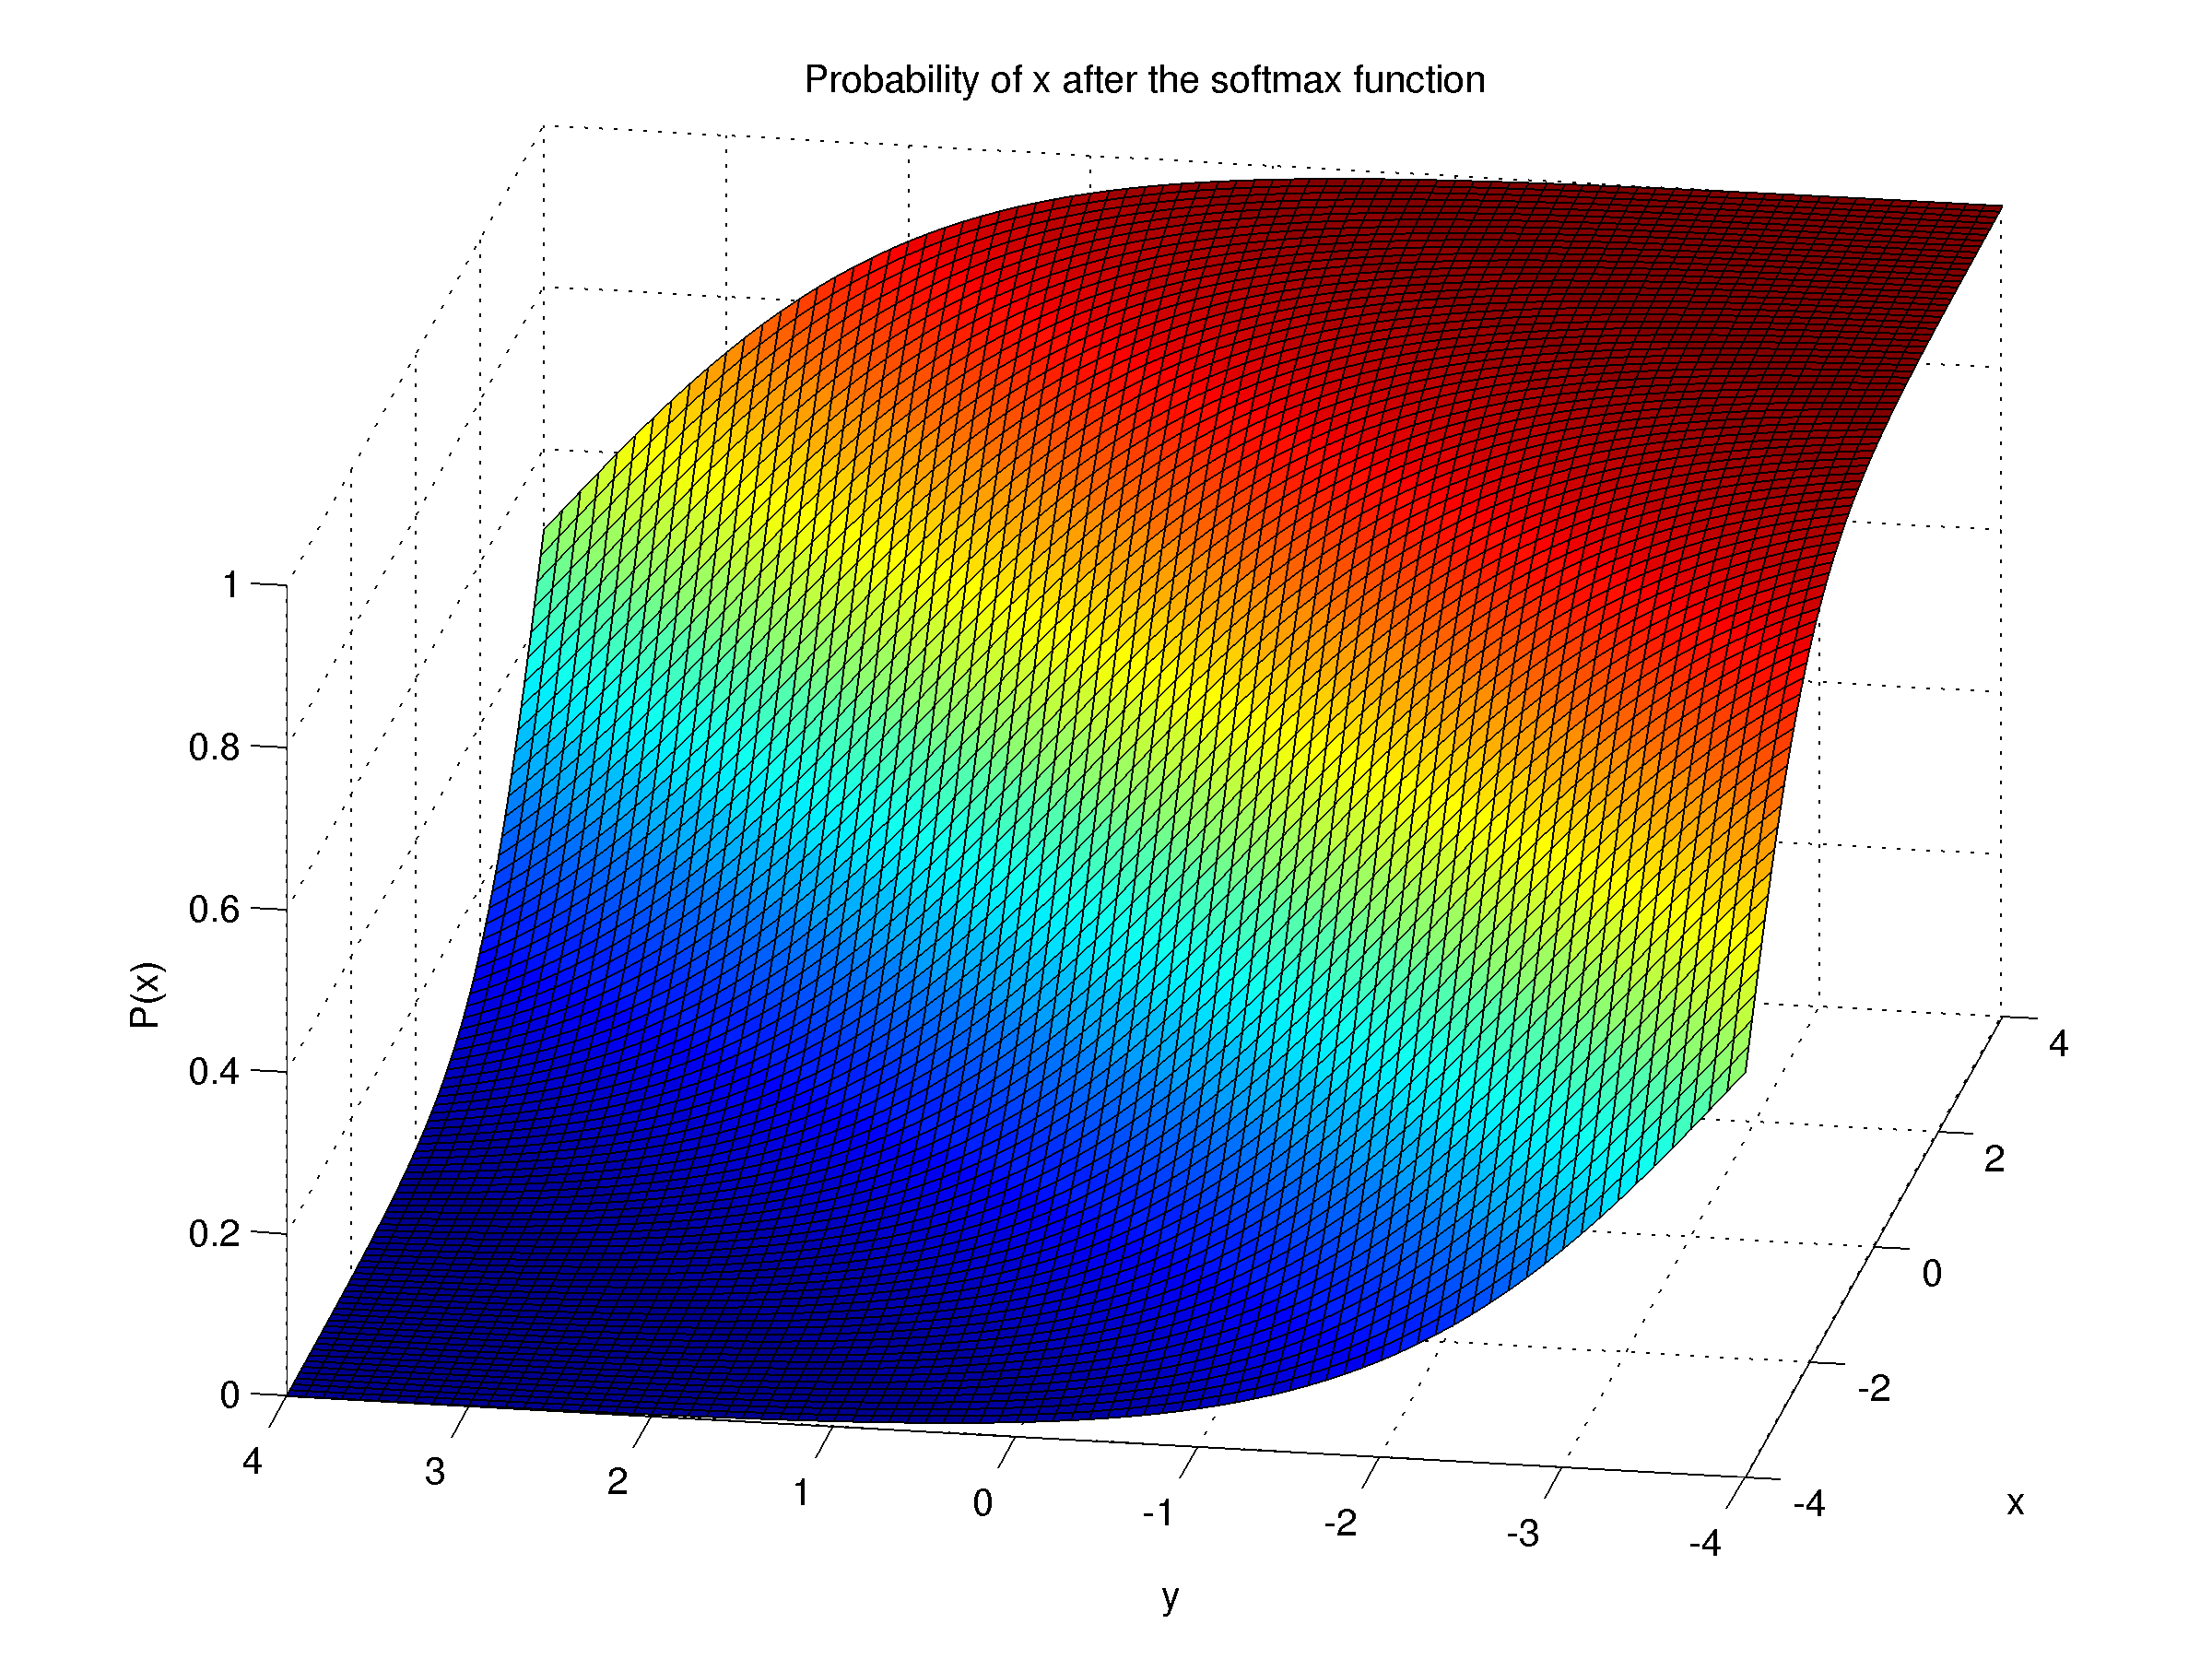
\includegraphics[width=0.9\linewidth]{twovarsoftmax}
  \caption{A visualization of the two variable softmax function. $x$ and $y$
  are the input variables and the output probability of $x$ is plotted. The
  probability of $y$ is just $1-x$.}
  \label{fig:twovarsoftmax}
\end{figure}


During training, the dot-product of the center and target word vectors 
is put into a softmax function to create a conditional probability: 
%
\begin{equation}
  \label{eq:softmaxwithdotprod}
  p(c|t)=\frac{\exp\left(v_{c,\to} ^{\quad\top} v_{t,\gets}\right)}
  {\sum_{w \in V}\exp\left(v_{w,\to} ^{\quad\top} v_{t,\gets}\right)}
\end{equation}
%
where $v_{w,\gets}$ and $v_{w,\to}$ are the input and output vector 
representations of $w$ and $V$ is the vocabulary. $c$ and $t$ are context word 
and target word respectively. So, this equation says that we 
treat the dot-product of two vectors as a weight\footnote{One function of the 
exponential in the softmax is to ensure there will not be any negative 
weights}. The closer together the vectors 
are and the longer they are, the greater the weight. We divide the weight for 
the context-target pair by the total weight of any vector with the target vector
to get the probability of the context word given the target word. In this way
the probability of any word occurring in the context of any other is encoded
in their vectors.

\subsubsection{Why Use Softmax}

Mikolov et al.\ do not explain why they chose the softmax function. Their 
reason could be as simple as a softmax activation function being a standard 
way to allow neural network outputs to be interpreted as probabilities in 
categorical estimation. However, an implicit model can be inferred by observing 
that the softmax function comes up naturally in probabilistic classification. 
As explained in, (\citealt{Bishop2006a}, pp. 197-199) for $K$ classes, the 
probability of class $k$ given an input is:
%
\[
 p(C_k | x) = \frac{p(x | C_k) p(C_k)}{\sum_{j=1}^{K} p(x | C_j)p(C_j)}
\]
%%
If we set $a_k = \log p(x | C_k) p(C_k)$ then the softmax function becomes 
obvious.
%
\[
 p(C_k | x) = \frac{ \exp(a_k) }{ \sum_{j=1}^{K} \exp(a_j)}
\]
$a_k$ has a particular meaning; it is the unconditional log probability of both 
events $C_k$ and $x$. That is, $a_k=\log p(C_k, x)$.

In \modelname{} the $a_k$'s take the form of a dot-product. Bishop notes that if 
you assume that the classes are Gaussian distributed with the same shape you get 
$a_k(x) = w_k^T x + w_{k0}$ where $w_k$ is a weight vector for a particular 
class and $w_{k0}$ is a threshold. If $\Sigma$ is the covariance matrix giving 
the common shape of the distributions and $\mu_k$ is the mean of the Gaussian 
for the $k$\textsuperscript{th} class,
%
\[
 w_k = \Sigma^{-1}\mu_k
\]
\[
 w_{k0} = ln p(C_k)-\frac{1}{2}\mu_k^T\Sigma^{-1}\mu_k
\]
%
In our case, $w_{k0} = 0$ so the squared length of the vector is related to 
the probability of the particular class and the weight vector for a class is
the class mean after it has been transformed into a space where all 
the class distributions are spherical.\footnote{Technically, where all of the
class distributions are hyperspherical.}

Mapping between Bishop's expressions and Equation \ref{eq:softmaxwithdotprod} 
gives us an implicit model. In Equation \ref{eq:softmaxwithdotprod} the classes 
are the context words and the $x$'s are the target, center words of the context.
So, if we randomly choose a word from the context and it generates an 
associated meaning-vector from a Gaussian cloud, the expression for determining
which context word generated that meaning-vector is exactly the probability
$p(c|t)$ given in Equation \ref{eq:softmaxwithdotprod}.

In other words, underlying \modelname{} there is a kind of continuous topic 
model where words generate topics in a meaning-vector space and the length of
a word's vector is related to how often it is chosen to select the topic 
as compared to other words in a context. \modelname{} selects the vectors for 
the target words so that the classification probability of which context word's
distribution generated that point in space matches the probability of that word
appearing in the target word's context.


\subsubsection{Hierarchical Softmax}

The softmax function in Equation \ref{eq:softmaxwithdotprod} above would work 
for training. However, to calculate its 
gradient (needed for optimization) you need to evaluate a sum over all words
in the vocabulary. Since vocabulary sizes are frequently large (on the order of
tens of thousands to tens of millions of terms) this takes too much time when it
needs to be repeated for every word in a several billion word corpus. Thus, 
\modelname{} uses hierarchical softmax.

\todo{rewrite to get rid of the redundancy with the overview section}
Hierarchical softmax decomposes the output procedure into a binary tree. All
words are placed as leaves on the tree. Then, rather than each word getting its 
own output vector, its ancestors on the path to the root hold several output
vectors that combine to calculate its probability with any other vector.

To define the equation for hierarchical softmax, we need to introduce some 
notation relating to the tree. First, we define the unique path from the root
to a word $w$. $n_{w,j}$ is the $j$-th node on that path and $L(w)$ is its
length. Thus $n_{w,1}$ is the root and $n_{w,L(w)}$ is $w$. We will designate
one of the children of each node as special (it will be given a positive 
weight). For each child node $n$, let $sp(n)$ be 1 if it is the special child
of its parent and $-1$ otherwise.
Finally, $\sigma$ will denote the standard logistic sigmoid 
$\sigma(x)=1/(1+exp(-x))$. Because 
the output vectors are associated with the inner nodes and the input vectors 
with the leaf nodes, it would be possible to dispense with the cumbersome 
input-output vector notational distinction. However, I keep it for 
comparison with the non-hierarchical formulation. With
these definitions, we can write the conditional probability of a context word
given a target word as:
%
\[p(c|t)=\prod_{j=1}^{L(c)-1} \sigma\left(sp\left(n_{c,j+1}\right)
\cdot v_{n_{c,j},\to}^{\quad\top} v_{t,\gets}\right)\]
%
It can be verified that for all $t$, $\sum_{c\in{}V}p(c|t)=1$. Now, the cost
of computing $\log p(c|t)$ and its gradient is proportional to $L(c)$, which, 
for a reasonably balanced tree is on average no greater than $\log |V|$. Most
implementations of \modelname{} follow \citep{Mikolov2013c} in using a binary
Huffman tree because its assignment of short codes to frequent words speeds
up training.

\subsubsection{Training}

Training begins with all of the inner node vectors initialized to 0 and the 
leaf node vectors initialized randomly on the $[-0.5\ldots0.5]$ hypercube. Then
for each pair of context and target words, the gradient is calculated and the 
vectors are moved to reduce the error. The size of these moves is controlled 
by a learning rate parameter that starts large at the beginning of training and
decreases linearly so that the iteration after the last training sample would
have a learning rate of 0. This causes the model to make big moves when the 
vectors are mostly random and, as it converges on a good solution, to make finer
adjustments.

There have been a few variants to this training procedure reported. 
\citep{Wolf} used batch updates to speed up training - accumulating the gradient
for each training sample but waiting until a certain, small number of training 
samples had been observed before updating the vectors. \citep{Perozzi2014}
proposed using the method in an on-line, streaming context which would require
removing the linearly decreasing learning rate because the number of training
samples would not be known in advance.

\subsubsection{Importance Sampling}

The size of the context used in the Skip-gram matters. Increasing context tends
to increase the quality of the model. However, increasing context also increases
training time. Further, the more distant words are less relevant to the current
word. So, instead of uniformly sampling the space of skip-grams when training,
a subset focusing on the words near the center is used. In particular, For each
target word, the algorithm selects a random integer $R$ in the range 
$[1\ldots{}C]$ where $C$ is the maximum context size. Then the context words 
at distances less than $R$ are used to train that target. 

\section{Principal Components Analysis (PCA) and Factor analysis}

When studying a system, it is common to believe that the observed
characteristics of that system are due to a number of unobserved, hidden 
factors. For example, one might believe that views on the importance of
economic equality, on the desirability of gay marriage, and on whether human
activities are causing global climate change are related because they are 
manifestations of an underlying political viewpoint. This underlying viewpoint
is not directly observable, so it must be hypothesized as an underlying factor.

Factor analysis is a set of tools which allow one to summarize a number of
variables using a smaller number of variables \citep{Bartholomew2011}. In this 
context, summarizing usually means that the new set of variables can account 
for most of the variation in the original set. And, though some techniques like
kernel-PCA are able to deal with non-linear relationships between the original
variables and the latent factors, most techniques seek factors that are
linearly related to the original variables --- for computational 
tractability, for ease of interpretation, and because the less flexible linear
model is more forgiving with respect to overfitting.

\subsection{PCA}

\begin{figure}[tbp]
    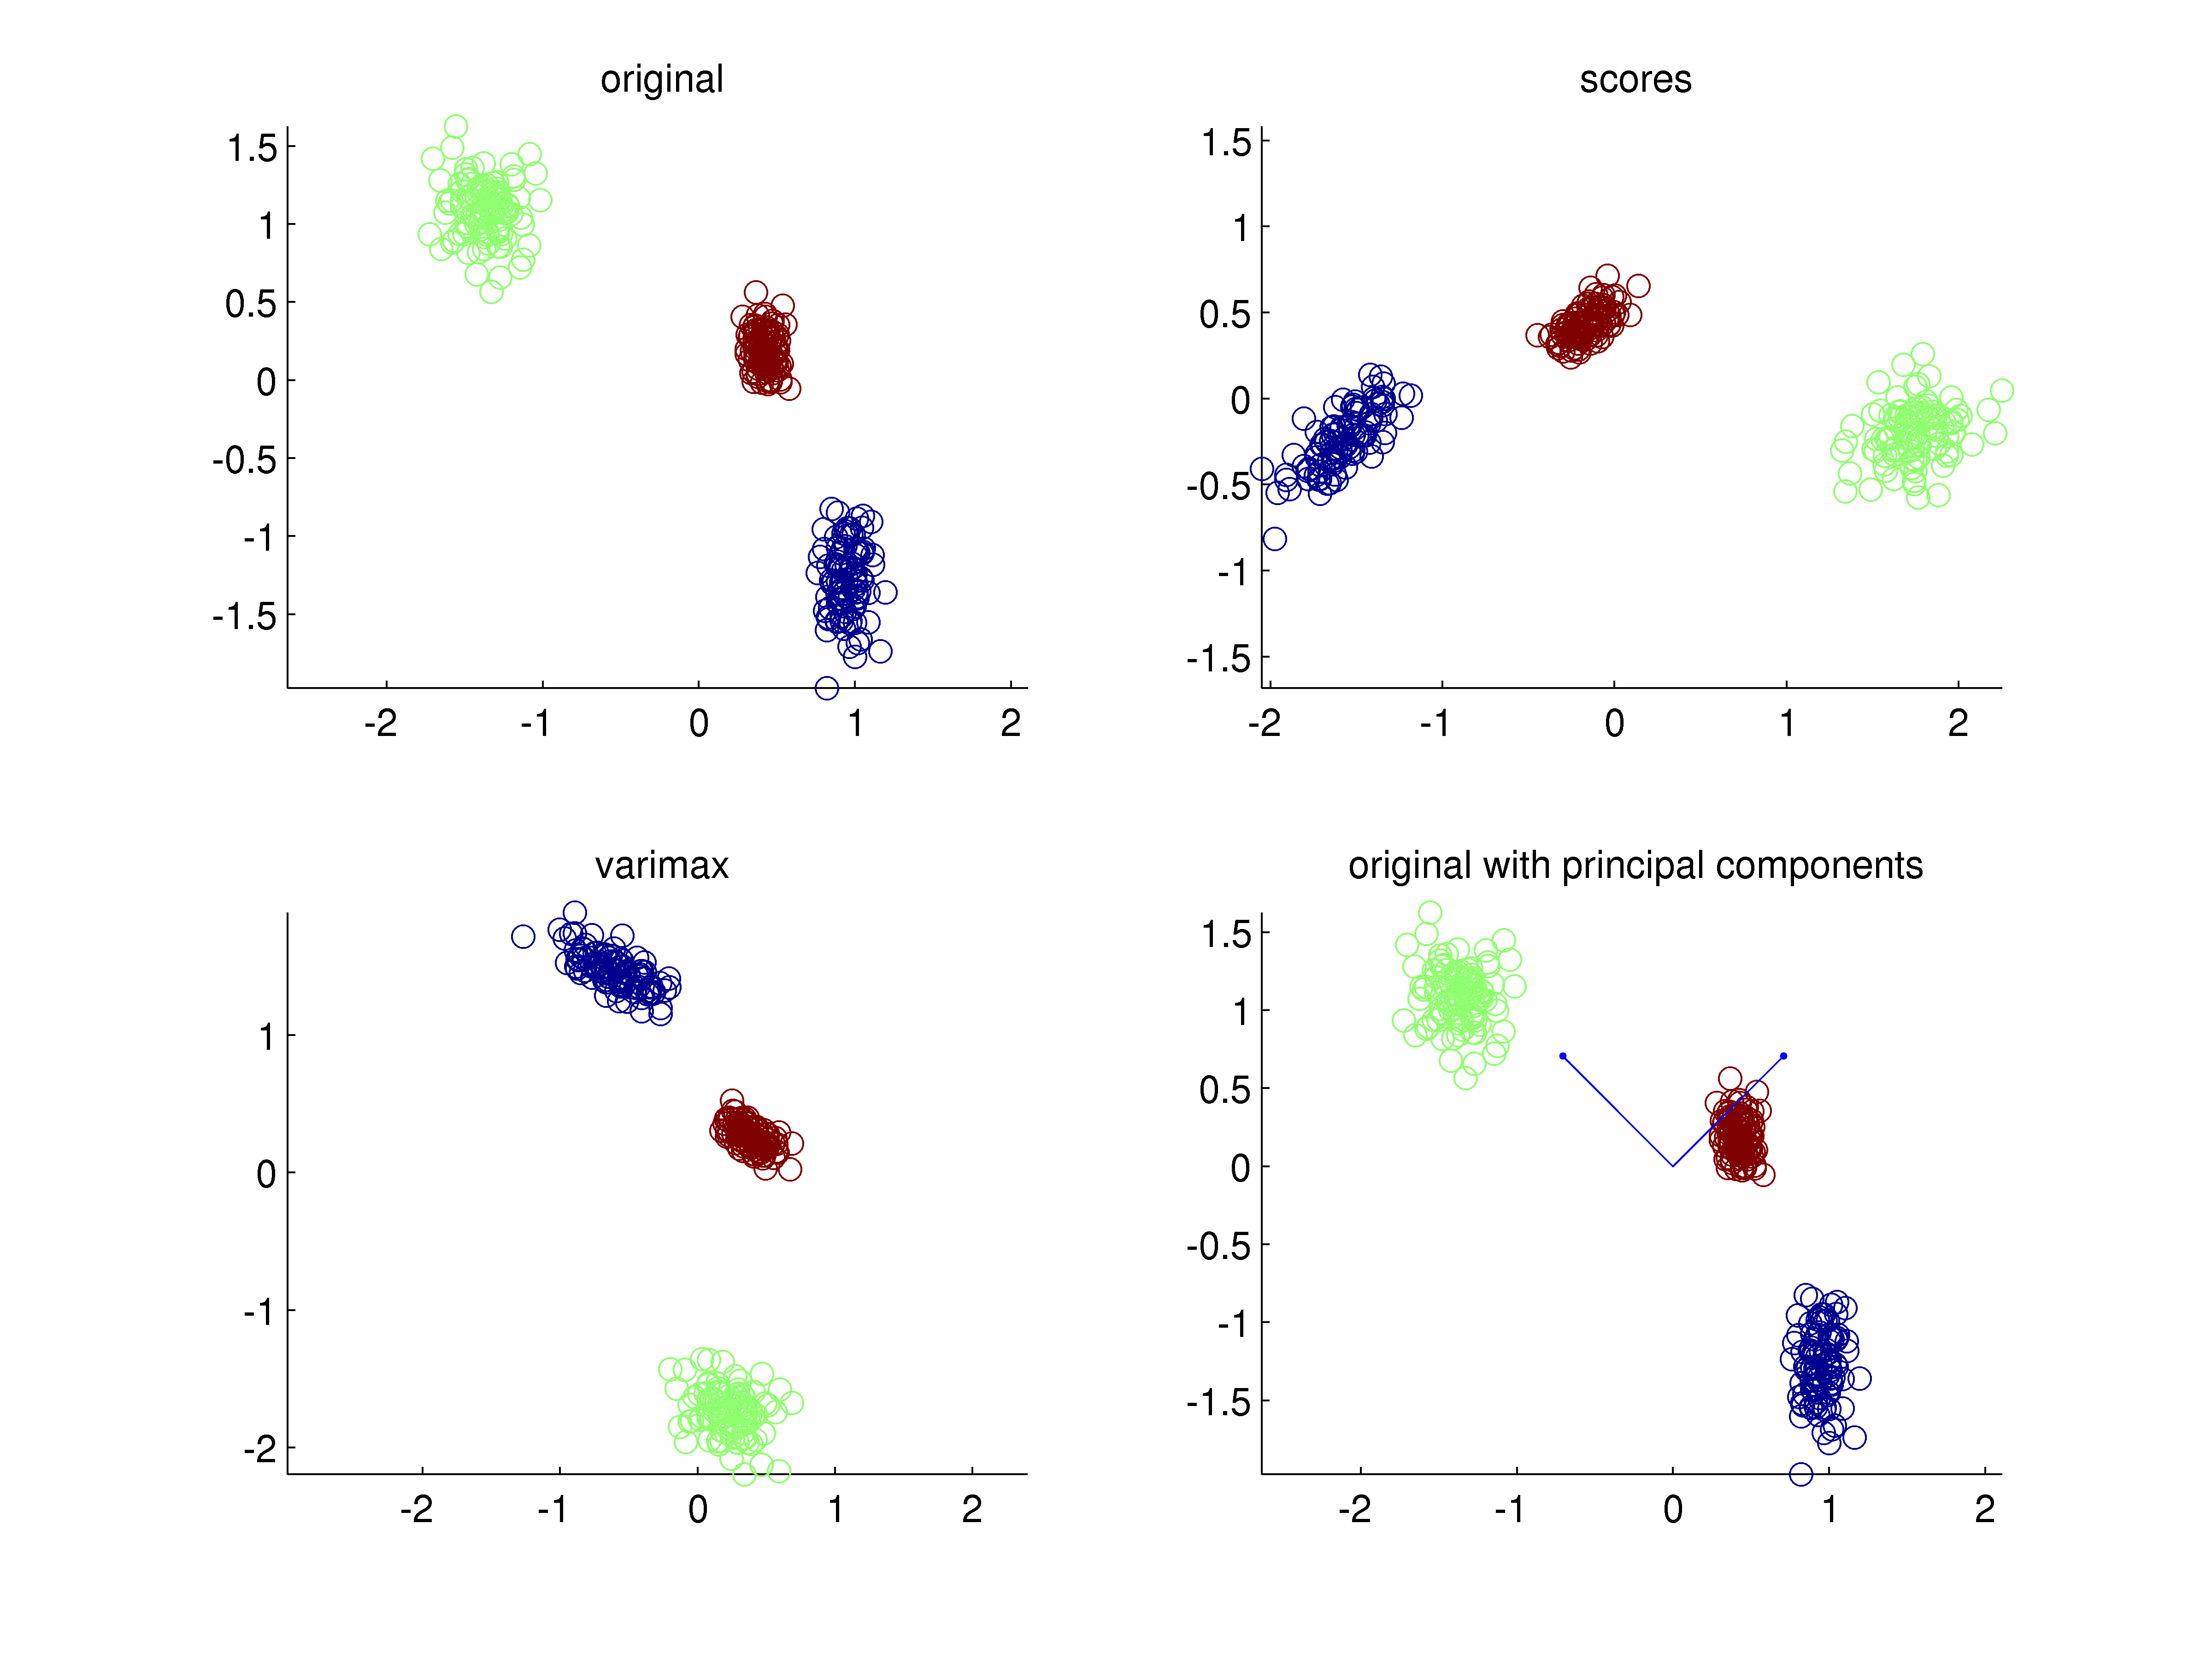
\includegraphics[width=0.9\linewidth]{factor_analysis_rotations}
    \caption{Diagram showing the effect of different rotation methods. 
    \textit{Upper left:} A dataset with three Gaussian clusters. 
    \textit{Upper right:} The scores plot, that is, the original points 
    redrawn in the new, rotated coordinate system of their principal 
    components \textit{Lower left:} The same points after varimax rotation. 
    \textit{Lower right:} The points drawn as they were
    in the original but with the principal components superimposed as arrows.}
    \label{fig:pcarotation}
\end{figure}

If you define a good summary as ``one which captures most of the variability'',
use a linear relationship, and measure variability as
variance then PCA is frequently your first step in factor analysis.
PCA finds a new set of axes for a set of input vectors so that the first
axis captures the most variance, the second is aligned with the direction with 
the second most variance and so forth. These new axes are the principal 
components of the input dataset and all of them are perpendicular to each other.

Figure \ref{fig:pcarotation} displays
graphically the effect of PCA. The upper left shows the original data. The
lower right shows the principal components derived from that data. Finally,
the upper right shows the original data after being rotated so the first
principal component lines up with the horizontal axis. This type of projection 
onto these axes is called a scores plot. It is easy to see that
this new x axis captures more of the spread of the data than either of the 
original two axes. This new axis is a new variable, a single latent factor that 
explains most of the variance in the original data.

Note that though this latent variable model captures an important factor in the 
data, it does not capture all the structure. This data was generated as a 
mixture of three two-dimensional Gaussians, so a perfect model would involve 20 
parameters: the center and covariance matrix for each cluster and the 
probability of generating a point in that cluster\footnote{The center and 
covariance matrix together are 6 parameters per cluster. This accounts for 18 
parameters. Only two mixing probabilities are needed because the probabilities 
must sum to 1, so the total is 20.}. The model we used is linear but the process 
generating the data is nonlinear.

A common variation on PCA is used to capture the covariance of several 
variables. To motivate this variation, imagine a dataset where one variable 
ranges from 0 to 1,000,000 and the rest from 0 to 1. It is easy to see that just 
choosing the large variable will capture most of the variability. However if you 
are interested in the relationships between the variables, their covariance 
structure, this will be hidden by the poor scaling. The solution to this is to 
z-score normalize all of the variables by subtracting their mean and dividing by 
their standard deviation. In that case the variance of each variable will be 1 
and PCA will pick out the axes with the greatest covariation.

\subsection{PCA and Matrices}

Because PCA performs a rotation, it can be looked at as a matrix factorization. 
It produces two matrices. If the input matrix contains observations (or 
individuals) in the rows and measured variables in the columns, the resulting 
matrices can be characterized as follows. The first matrix is the loadings 
matrix, which has rows that are factors and columns that correspond to 
variables. The second is the scores matrix, which has columns that are factors 
and rows that are observations. 

The scores matrix represents the observations (or individuals) expressed in 
terms of the new latent factor variables. The loadings matrix gives the 
relationship between the original variables and the new factors, allowing one 
to be expressed in terms of the other. It is conventional to write the loadings 
matrix so that the factors are unit vectors to make them a unit basis for the 
new space. The separation into loadings and scores is a matrix factorization 
because if you multiply $scores \times loadings$ you get the original matrix 
back. Further, because the principal components are ordered in terms of variance 
captured, if you choose the first n rows of the loadings matrix and multiply 
them by the first n columns of the scores matrix, you will recover an 
approximation to the original matrix that is the best approximation\footnote{The 
approximation is best in a least-squares sense.} that can be made with n 
underlying dimensions.

\subsection{Interpreting the factors}

\subsubsection{Choosing the matrix}
Though machine learning practitioners will seek principal components merely as 
a dimensionality reduction strategy, in the sciences, factors are sought 
because the seeker wishes to understand the system. This requires interpreting
the factors. Either the scores or the loadings matrices can be used in this 
interpretation. The loadings matrix relates factors to the original variables
and the scores matrix relates factors to the original observations. 

Which matrix is chosen for interpretation depends on whether the analyst can 
extract more meaning from the original variables or the original observations. 
For example if the original experiment matched radio frequency emissions with 
rats from two groups at two different times, ``intensity at 300Hz'' carries less 
semantic information about the question under study than ``rat given placebo at 
time 2'', so the analyst would use the scores matrix. On the other hand, consider 
the case where the observations in the experiment were of random people and the 
variables were ``Is gregarious'' and ``Is helpful.'' ``Is gregarious'' has more 
content relating to personality than ``random subject 2011 - male,'' so the 
analyst would use the loadings matrix.

\subsubsection{Creating the interpretation}

\label{sec:bg:factorinterpretation}
Once the appropriate matrix has been chosen, one can use the factors directly
and just look at the highest loading/scoring components (as was done in 
\citep{Samsonovich2010}). However, it is
also common to rotate the factors according to a criterion that makes 
interpretation easier - for example, varimax rotation. Thresholds for a 
significant loading/score are also used. At the end, the analyst has for each
factor a list of items (variables or observations) that are highly ranked for a 
factor and a list that rank poorly on that factor. Based on the meaning of the 
two groups, the analyst can hypothesize what differentiates them that could also
be reflected in the original data and then assign that interpretation to the 
factor.

\section{Lexical Hypothesis in Personality Psychology}

After the \modelname{} model and factor analysis, the third piece of background
crucial to understanding my work is the lexical hypothesis in personality 
psychology.

As mentioned in Section \ref{sec:personalitymodelsfromvectors} there are many
methods for formulating personality models. One approach is to attempt to extract the 
intuitive personality model held by most people. It can be assumed that this
model is reasonably good because our species, being very social, needs to 
interact with and model others as a condition of survival. 

A good way to try and get at this model is to use language. The lexical 
hypothesis in psychology is:
``those individual differences that are most salient and socially relevant in
people's lives will eventually become encoded into their language'' 
\citep{Goldberg1982} This approach was initially proposed by 
Galton \citep{Galton1884} and was pursued by psychologists for the following century
but it made its most significant gains in popularity after an influential seminar
by Goldberg in 1983. \citep{Deary2009}

\subsection{Word lists}

As stated, the lexical hypothesis covers the encoding of personality traits in
all of language. However, as implied by its name, psychologists working from 
the lexical hypothesis have focused on finding personality in the vocabulary
of the language rather than in its grammatical structure. Galton pioneered this
as well, spending time with Roget's Thesaurus and coming back with an estimate
of 1,000 applicable words. \todo{cite Galton 1884 p. 181 
``Measurement of Character'' Fortnightly Review} 

The next notable advance in word lists was reported by Allport and Odbert \todo{ref cite
Allport and Odbert} who tabulated 
all the trait names in the
Webster's unabridged New International Dictionary. By their count, there were
17,953 terms. They chose words that had the ``capacity ... to distinguish 
the behavior of one human being from that of another.'' Thus, they excluded
words which specified non-distinctive behavior. Because they were
mainly attempting to create a list in which the entries could be rough proxies
for traits, they attempted to reduce redundancy by avoiding nominative and
adverbial forms and including multiple words from clusters where they judged 
that the different forms arose because of arbitrary morphological development 
rather than reflecting semantic distinction. Thus \textasciitilde 18,000 terms, frequently taken to 
be an approximation
of the number of personality terms in the English language is actually an
underestimate.

Allport and Odbert divided their list into 4 categories. The first was the
closest embodiment of the most clearly ``real'' traits of personality. ``They
designate generalized and personalized determining tendencies - consistent and
stable modes of an individual's adjustment to his environment.'' The other three
categories included words that were more temporary, more censorial, and more
metaphorical and remote in their applicability to personality.\footnote{ 
It is interesting that our automatic software includes as some of its most 
important dimensions ones that could be used to categorize words on two of these
axes.
There is a positive-negative component and a ``frequently applies metaphorically''
component. The lack of a component measuring temporariness is not surprising
since the word-list we used excluded words designating temporary states.}

Word lists of the size generated by Allport and Odbert were too large to use 
with statistical techniques before the advent of computers. So, Cattell \todo{
ref cite Cattell 1947 Confirmation and clarification of primary personality
factors} manually reviewed the list and chose 35 trait variables he felt
summarized the words in Allport's first category trait list. This list is
notable because Cattell used it to produce his influential 16 factor model
and an independent analysis by Tupes and Christal in 1961 \todo{cite ref Tupes 
and Christal 1992} is the first clear recognition of the five factor 
model.

The last of the massive dictionary-derived trait lists was published by W. T. 
Norman in 1967 \todo{cite ref Norman1967}. He started with all 4 categories of
Allport and Odbert's list and added all words that ``pertained in any
manner to attributed of persons or their behavior but which were not included 
in the Allport-Odbert list'' from Webster's Third New International Dictionary
Unabridged (1961). Then, in a first culling, a group of four raters removed 
the most obscure words, 
those that were
nebulous and extremely metaphorical, physical aspects of behavior, movements,
location, or of appearance, grooming and dress, and finally those which are
purely evaluative, or qualifiers of degree. Next he
classified the remaining words into 15 categories roughly indexing their
stability/temporariness, formality, commonness, reference to social constructs
\footnote{Words like adversary, helpmate, outcast were high in this category}
and then the 4 categories from the first, rough cull. He kept the stable words
that did not refer to social constructs as his list of 2800 trait words. His
list did not restrict itself to adjectives.

After Norman, people continued to produce word lists for trait evaluation. But
many of them were much smaller \textendash designed for use in direct personality 
assessment and they are frequently dependent on one of the earlier lists. We
use two such lists from Goldberg in our later analysis. \todo{cite ref Saucier
and Goldberg 1996 (for 435 words) and Goldberg 1990}

\subsection{Factor-analytically derived traits}

The lexical hypothesis is one of the most important hypotheses in personality
modeling today. But to be useful, the information about personality structure
cannot remain diffused throughout lists of personality words but must be 
extracted and condensed. Starting with Cattell in the 1940's \todo{cite cattell
1948 as an example} research psychologists turned to factor analysis to 
concentrate the information about personality contained in language into usable
knowledge.

The general method for producing a list of traits through factor analysis is to
measure many variables which one believes are related to personality. Then,
factor analysis will produce clusters of variables that score high or 
low\footnote{usually a cut-off of 
$\left|v\right| > 0.3$ or $\left|v\right| > 0.4$
is chosen for high/low loadings, which means between 9 and 16 percent of the
variance of that variable is accounted for by that factor.} on
a particular factor. These are then used to help the experimenter interpret
that factor as a trait summarizing an important aspect of personality. 
A large majority of studies on personality models 
refer to the Big Five structure \todo{ref cite Boele De Raad 
``Structural Models of Personality'' 
p.127 chapter in ``Cambridge Handbook of Personality Psychology''} which was
derived from just such a factor-analytical approach to the lexical hypothesis.

\subsection{Biological basis}

Relying only on a lexical approach does not give the whole picture. It is more
descriptive than predictive. It is like recognizing that the sky is blue on a
clear day and gray on an overcast day. It is an accurate assessment but it does
not describe the mechanism that produces blueness and grayness. 
We know that gregariousness and warmth are 
correlated when people describe others and we attribute this to differing
quantities of a trait called extroversion. However, whether this trait of
extroversion comes from genes, from universal actions mothers take with 
infants or from quirks in human social perception is not specified.

One way to address this shortage is to take existing lexically-based models and
attempt to find a basis for the observed regularities. There is continual work
attempting to find a biological or genetic basis for the Five Factor Model.
Recent successes showed that the factors are heritable \todo{ref cite Riemann,
Angleitner and Strelau 1997} and that some genes influence both warmth and 
assertiveness - explaining why both covary as facets of 
extroversion. \todo{cite ref Yamagata,
Suzuki, Ando et. al. 2006 and Pilia, Chen, Scuteri et al. 2006}

Another way to attempt to add biological information to personality traits is
to guide your factor analysis using biological information. Such an approach
was taken by Eysenck who started with biological hypotheses that two very 
important personality traits were extroversion and emotional stability and
then used that to guide his factor analysis which tested how good his theory
was.\todo{cite ref Carducci 2009 The Psychology of Personality Second Edition 
p.284}

\chapter{Related Work}

\section{\modelname{} model}

There has not been a lot of time since the publication of the \modelname{} model. 
However, in that period, researchers have attempted to improve its algorithms
and vector quality, and also created applications, both within and outside 
Natural Language Processing (NLP). It has also seen use as a 
standard reference to which the performance of other algorithms is compared.

\subsection{Algorithm and Vector Improvements}

\citep{Mikolov2013c} tested alternative training procedures. They tested an 
alternative to the hierarchical softmax used in the \modelname{} model called 
negative 
sampling. The also tested a way of giving less weight to frequent words
which speeds up training. The weight adjustment improved the resulting vectors
more than negative sampling. They also demonstrated a simple method
of extracting phrases whose meanings were not simple compositions of their
component part meanings and extended their semantic test suite to use some
of these phrases.

\citep{Faruqui2014} created a method using CCA (Canonical Correlation Analysis) 
to take vectors generated on
monolingual corpora for different languages and combine them to create new sets
of vectors utilizing the semantic information from both. They then compared the
semantic distance mappings thus obtained to several sets of human-labeled 
semantic distances. They also used the analogy tasks from \citep{Mikolov2013a}.
With LSA as the source for the original vectors, they were
able to uniformly improve performance on all measures. Similarly, with a
Recursive Neural Network (RNN) as the source of the vectors, there was less
improvement, but still only a loss on one task. Vectors from \modelname{} 
however had no detectable change in most cases but their performance decreased
on the same task as the RNN\footnote{The authors do not mention having done
multiple test correction, so their significance values may be invalid.}.

\citep{Wolf} also created an extension of \modelname{}\footnote{They use the
Continuous Bag-of-words architecture rather than the Skip-gram variation I
use.} that takes advantage of
bilingual information to to improve vector quality. They believe it works 
because it deals better with polysemy, since it is rare that homographs of 
translations cover the same set of senses. They require a word-aligned 
training corpus and use a vocabulary 
composed of all words in both languages. They first train the model on both
languages as usual. Then, they train the words using the context from the 
matched opposite language word. So, for example, the word 
``ran'' is aligned with the word ``corri\'o'' in the two parallel sentences 
``She ran to the store'' and ``Ella corri\'o' a la tienda''. So the context of 
``ran'' in the second phase would be ``Ella,'' ``a,'' ``la,'' and ``tienda.''
\footnote{Because their Hebrew-English parallel text pairs the 
Hebrew Bible with its King James translation, one of their tests involves 
synonyms taken from Strong's 1890 
concordance. Many people believe that
all the senses of a word are expressions of some ``root meaning'' of that word 
and so
pick and choose glosses from Strong's dictionary to give other nuances they 
believe were held by the 
original Greek or Hebrew that did not make it into English. This makes 
Strong's work an ironically appropriate choice for this study 
since this ``root meaning'' assumption is almost the same as the assumption that 
vector-space language models impose by assuming a single point for each word 
and which the authors are trying to overcome by using multiple languages.}

\citep{Bordes2013} extended the implicit linear operators expressing 
relationships in \citep{Mikolov2013b} and explicitly trained a vector
space representation of RDF-type triples 
$(subject,predicate,object)$ that 
capture the semantics of $predicate$ by attempting to make 
$subject+predicate \approx object$ when the predicate holds and make it
far away otherwise. The resulting model is able to predict links better than
several more expressive models by the same authors on both Freebase and 
WordNet datasets. And even when the link predictions do not contain the best
answer, they reflect common sense.

\subsection{Applications}

\citep{Mikolov2013a} creates a method of generating phrase tables and 
dictionaries from two languages with only a small amount of bilingual data.
They first train the \modelname{} model on two independent monolingual corpora 
and then align the vector spaces with a linear transformation derived from a 
small number of matched word pairs. The resulting translations had the 
correct word within the top 5 candidates (which were usually synonyms) 90\% of 
the time.

\citep{Frome2013} used \modelname{} vectors as the targets in a second round
of training a state-of-the-art image recognition convolutional neural network.
The semantic generalization afforded by the vector space structure allowed them
to predict labels for images where it had never seen an image with that label
at all\footnote{There were 1000 labels in the training set and 20,841 unseen 
labels not included in the training set images.}. Later, almost the same team 
published \citep{Norouzi2013} which 
generalized the method to allow use of any n-way image classifier and to 
remove the requirement that the classifier had to be retrained using the 
new output structure. 

\citep{Perozzi2014} created an algorithm called DeepWalk which uses
\modelname{} to assign representations to nodes in a network graph. First, 
random walks on the graph starting at a given node are generated. Each node is
treated as a word and each walk is treated as a sentence. These are then run
through the \modelname{} algorithm to produce vectors that describe each node.
Despite the fact that the vectors are generated using only local information
about the graph, on multi-label classification problems they were able to 
outperform competing techniques that required
a global view of the network - with the competitive advantage increasing with 
the sparsity of the labeled training data. They proposed an on-line version of
the algorithm and one that could capture additional relationships by looking at
non-random paths through the network generated by users.


\citep{Osendorfer2013} proposed using \modelname{} vectors in an information
retrieval setting for computing similarity between musical pieces. Looking at 
music as a language, they intend to use the sparse translation technique from
\citep{Mikolov2013a} to translate between normal language and music.

\section{Studies involving both topic models and personality}

To my knowledge, no one has yet attempted to derive the structure of personality
words by looking at the components of a vector-space model. And 
I am certain no one
has attempted it with vectors from the \modelname{} model. 
However, that does not
mean that the subjects of vector-space lexical semantics and personality are
completely disjoint. I located a number of articles where both played a role.
Most were attempts to predict personality or some aspect thereof from some body 
of text like emails or tweets. There was also one paper that used topic
models as an exploratory tool, attempting to discover more about personality.
A final paper, in deriving results about the structure of language,
found three dimensions that were consistent across different
languages and different source corpora. Of these three, at least two and 
possibly all are personality-relevant.

\subsection{Personality predictive models}

The majority of papers looking at both vector-space language models and 
personality are attempts to predict personality or some aspect thereof from a 
body of text.

\todo{cite Shen Brdiczka Liu 2013} build a classifier to predict three levels
(high, medium, and low) of each of the Big Five personality dimensions from
individual emails using hand-selected features. One of the underlying 
probabilistic models they reject is an LDA variant. Their final classifier
achieves around 70\% accuracy.

\todo{cite Hill, Song, Dong 2001} use LSA on a collection of design documents
to produce vectors which they separate into components one coming from 
the author's, speaking personality and the other from the topic of the document.

In \todo{cite Gill and French 2007} the authors attempted to predict personality
using three different vector space lexical semantic models including LSA. These
models were trained on several standard news and academic corpora. They
had emails from students who had taken the Eysenck Personality Questionnaire and
tried to predict their extroversion and neuroticism by looking at the similarity
of their emails to 10 prototypical words ``defining a trait'' from \todo{cite ref 
Goldberg 1992 Development of markers for the Big-Five factor structure} and
by looking at the 7 words that were most frequent in emails from the people who
were most extreme on the given traits. The semantic models failed on both
counts while human raters were able to reliably predict both extroversion and
neuroticism from the same texts. They concluded that topic models do not
extract the right kind of information to classify personality. An external
observer, however, might note their unsophisticated use of pre-made topic
models created in a different domain to examine poorly selected features in 
a very small list of documents as an alternate explanation for their failure.

In \todo{cite Arvidsson Sikstrom and Werbart 2011} they use LSA to show that 
psychotherapy causes changes in a self-report-based personality index based 
on a patient's description of himself, his mother and his father.
\footnote{I was unable to access the full text of this article before I
had to submit the thesis but I still felt that the article was likely 
relevant.}

\todo{cite Pennacchoiotti2011} uses a large number of features including topics
from different LDA models to predict various features of Twitter users including
political orientation, which may be considered a correlate of the openness
personality dimension.

\subsection{Questions in the study of personality}

Besides these predictive studies, one article used vector-space lexical 
semantics as a tool to explore personality. \citep{Schwartz2013a} use a 
database of 14.3 million posts from 75,000 
Facebook users who took a Five Factor questionnaire and analyzed their Facebook 
posts to gain insight into gender, age, and personality. One of the features 
they examine is topics from an LDA model. Their personality-sorted results
mainly looked at N-grams (which produced the novel observation that introverts
like Japanese culture). Their insights from the LDA were mainly about lifespan
issues. For example, social
topics increase with age and antisocial topics decrease.

\subsection{Serendipitously discovered personality factors}

Possibly the most relevant work is \citep{Samsonovich2010} (which is an
expansion of \citep{Samsonovich2007}). In this work the authors are not
intending to discover anything about personality, rather they are investigating 
the semantic structure of language. They
analyze synonyms and antonyms in English, French, and German. In all three
languages, they discovered that the first three principal components could be
summarized as measuring positive/negative (valence), strong/weak 
(dominance,arousal), and open/closed (freedom). They used a similar criterion
to Mikolov for constructing the space in that they minimized a cosine distance
for close words. But because of the presence antonym information, they were
also able to specify that antonyms should have maximum cosine distance.
The resulting vector assignments had 4 obvious and strong principal
components, of which 3 were replicated across languages. Because of the
underlying human-generated synonym-antonym classification, the generated
categories better reflect the way humans divide up the world. Additionally,
the first two categories are similar to several two-factor personality models:
Morality/Dynamism \todo{ref cite Saucier, Georgiades, Tsaousis, and Goldberg 2005}
or Virtue/Dynamism \todo{ref cite De Raad and Barelds 2008}. The authors also
see a similarity between their factors and Communion/Power from the 
interpersonal Circumplex of Leary \todo{ref cite Leary T (1957) 
Interpersonal diagnosis of personality. New York: Ronald Press}. This suggests
the 
interesting possibility that the great cross-cultural similarity in personality
factors comes in part from the fact that humans, the main measuring instrument,
classify \textit{everything} along these two dimensions. It would be a very
interesting follow-up to look at the portion of semantic space generated
from these thesauri inhabited by personality words and see what other 
dimensions are present when the noise of multiple, overlapping topic-areas
is removed.

\documentclass[eric_thesis.tex]{subfiles}
\begin{document}

\chapter{Methods}

\section{Corpus: WMT11}

For training, we used the English WMT11 corpus. This is a training set collected 
for an academic competition at the sixth workshop on statistical machine 
translation. It is composed of minutes of the European parliament, news 
commentary, and news articles collected by the common crawl in the years 
2007-2011\todo{ref wmt web page, wmt citation (if any), and common crawl 
citations for appropriate years}. The European parliamentary minutes are in 
readable order. The news articles have been broken into sentences and those 
sentences included in random order\footnote{I have not read the rationale for 
this, but I believe that it was done to preserve intellectual property rights.}. 
All of the WMT11 corpus is broken into single sentence lines. Enclitics have 
been separated so ``don't'' is written as two words ``don'\phantom{}'' and the 
single letter ``t''.

We chose to use the WMT11 corpus because it was both large (several billion 
words) and had already been used with the skip-gram model in \todo{the paper on 
language translation with the skip-gram}. Additionally, it had been originally 
compiled for a competition, this assured that much preprocessing had already 
been done.

\section{Preprocessing}

Despite some preprocessing having been done, as is customary in natural language 
processing, we still needed to do additional preprocessing to normalize the data 
for our purposes.

\subsection{Filter angle tags}

The first step we took was to remove spurious HTML and SGML tags that had been 
accidentally left in the data by the common crawl acquisition software. Most of 
the data is plain text. However, sometimes the software downloading the news 
stories did not parse the HTML correctly or the source material had erroneous 
HTML that confused the parsing software. Thus the plain text files were 
corrupted by portions surrounded by angle brackets like <P>. There were also 
stock-ticker symbols and other miscellaneous garbage included. These symbols 
would show up as words, but they are not English words and, being remnants of 
the download algorithms, are used inconsistently. To remove this digital 
flotsam, we wrote the script \filename{filter\_angle\_tags.pl} listed in 
Appendix \ref{app:filterangletags}.

We developed the script by first listing all the unique strings that began with 
< and ended with >, call each of these a tag. The function of some tags was 
obvious. For example, some were part of HTML. For each non-obvious tag, we found 
it in the corpus to determine its use from context. Then we appended it to a 
list of regular expressions to filter from the input before listing the tags. 
These filtered tags were grouped into two parts, ones we wanted to keep and ones 
we did not. When the output list was empty, we knew we had a regular expression 
covering every tag in the corpus. Then, finally, we transformed the regular 
expressions we wanted to remove into a script that would pass through only those 
regular expressions called \filename{check\_angle\_filter.pl} and created the 
\filename{filter\_angle\_tags.pl} program to remove that same group of regular 
expressions. We considered our work complete when the filtered corpus came up 
empty after being passed through \filename{check\_angle\_filter.pl}.

\subsection{Part-of-speech tagging}

An important limitation of vector based lexical semantics is its way of dealing 
with polysemy (absent mitigation techniques such as those in \todo{ref some 
mitigation techniques}). Since each word gets only one meaning vector, if the 
word has more than one meaning, its associated vector is some sort of compromise 
between all of the meanings used. In the case of personality words, polysemy is 
very common. For example, consider the word ``kind''. If used in the utterance, 
``What a jerk? Of course, John is kind.'', kind carries the meaning you expect 
on a personality survey. But if used in ``What course? John is kind of a jerk.'' 
it forms part of an adverbial phrase indicating an incomplete matching to a 
description. And if used in ``What? Jerk John is a kind of course.'', kind is a 
noun that is a synonym of species. Fully distinguishing the uses is a 
significant task. However, just marking the part of speech deals with a great 
deal of the polysemy. In the example above, only the adjective is a genuine 
personality word. 

Part of speech marking misses some subtle distinctions, such as when someone 
says, ``If <person> would be so kind.'' (a common phrase in the parliamentary 
notes). However, it is very good at broader meaning differentiation. We looked 
at the 438 words used in \todo{ref whatever paper the 438 words come from}. In 
the vast majority of cases, Wordnet had only one definition that had to do with 
personality and that definition was distinguished from the others by determining 
whether the part-of-speech was an adjective or not. For 6 words (cunning, 
daring, faultfinding, quiet, self-pitying, and understanding) both the adjective 
and non-adjective categories had a personality meaning. So, being an adjective 
correctly distinguished personality word semantics 98.6\% of the time.

After consulting with Dr.\ Katrin Erk, \todo{ref private communication with Dr. 
Erk} we used TreeTagger \todo{ref tree tagger paper} as our basic part-of-speech 
tagging engine. Because TreeTagger must load all sentences to be tagged into 
memory, it cannot deal with the entire corpus at once. So, we split the corpus 
into 14 files of 10,000,000 lines each (the last being smaller). TreeTagger 
(using the \filename{tree-tagger-english-utf8} script) processed these into 14 
files which had a single tagged symbol on each line. The splitting and tagging 
process was automated by our \filename{tag\_corpus.sh} script included in 
Appendix \ref{app:tagcorpus}.

\subsection{Reassemble corpus}

The 14 files were not in the single-sentence-per-line format needed by our model 
generation software. So, we wrote another script (\filename{reassemble\_tags.pl} 
Appendix \ref{app:reassembletags}) which took the 14 files, used the sentence 
ending tags to detect line ends and output only the original words except in the 
case of adjectives. Adjectives were output with an underscore and the tag JJ 
(which is the tag for an adjective used in the Penn Treebank \todo{ref penn 
treebank paper and paper giving the penn treebank tags if it is different}). So 
the word ``kind'' was output as ``kind\_JJ'' if it was an adjective.

Late in the research, we realized that \filename{reassemble\_tags.pl} did not 
put a newline at the end of the last sentence in its input file. Thus when the 
files were concatenated into the adjective-tagged corpus file, the 13 sentences 
ending the first 13 input files were concatenated with the 13 sentences starting 
the last 13 input files. Since this only affected 26 sentences out of more than 
1 billion, we decided it would not have a significant effect on the results. 
However, the version of \filename{reassemble\_tags.pl} in Appendix 
\ref{app:reassembletags} has this error corrected.

\subsection{Case folding}

For most words in English, capitalization does not affect their meaning very 
much. Much capitalization is just a marker of ``first word in the sentence.'' 
So, it is better to convert all words to lower-case. After reassembling the 
corpus, we converted all upper-case letters to lower-case. We did not convert at 
the beginning of preprocessing because capitalization is an important clue for 
part-of-speech tagging.

In a test run, we did not convert to lower-case. When we analyzed the resulting 
word-vectors, the most important component was capital versus lower-case. This 
is reasonable because the structure of the beginning of an English sentence is 
different from the structure of the rest of the sentence. For example, the 
beginning is usually the subject of the sentence. Thus, different words will 
appear at the beginning than at the end, and since capitalization frequently 
signals the beginning of the sentence, words in the subject are more likely. 
However, for the kind of meaning we want, whether a word begins a sentence is 
surplus information. So, we removed capitalization to suppress this kind of 
noise.

A disadvantage of case-folding is that some information is lost. For example: 
God and god become intermixed and Jimmy (noun) and jimmy (verb) are 
undistinguished. Almost the entire problem could be mitigated by including 
markers for proper nouns. However, it did not seem to be causing much problem, 
so we left that for later work.

\section{Number of Vector Dimensions}

Once we had the preprocessing done, the next step was to choose the number of 
dimensions in the vectors. The the vector dimensionality is an important 
parameter for any vector-based lexical semantics algorithm. For LSA, the number 
of vectors has a curvilinear relationship to meaning captured. In \todo{ref 
landauer and dumais 1987 see also handbook of LSA p.59}, performance on the 
synonym section of the TOEFL \todo{ref toefl} increased with number of 
dimensions up to about 300 and then decreased as more dimensions were added. In 
our case, we chose 800 dimensions because that was the best number of dimensions 
found for converting English to the similar language Spanish \todo{ref skip-gram 
translation paper} on the assumption that sufficient meaning to convert between 
those two languages would also be sufficient for capturing the most important 
personality dimensions.

\section{Create vectors and select words to PCA}

\todo{Add part about choosing a frequency cut-off to fit all the skip-gram 
vectors in memory}

Number of dimensions in hand, we generated the meaning vectors using the 
skip-gram implementation in gensim. \todo{ref gensim} Then we selected the 
meaning vectors (model.syn0) for our wordlists from the generated model using 
the script included as \filename{extract\_vectors.py} from 
\ref{app:extractvectors}. The lists of words were taken from three sets of 
personality words. 

\subsection{101 word list}

The first, containing 
101 words was taken from the list of 100 words in the paper \todo{cite paper 
from which the hundred words come}. To this, we added the variant spelling 
``extroverted'' because the spelling ``extaverted'', which was in the original 
list, did not appear in the WMT11 corpus. To match the words in the tagged
corpus, all of the words had the characters ``\_jj'' appended because the list
was intended as a list of adjectives and JJ is the standard suffix for adjective
used in the Penn Treebank \todo{ref cite penn treebank} and thus is the suffix
used by our part-of-speech tagging software.

\subsection{438 word list}

The second set had 438 words and was 
taken from \todo{ref cite paper from which the 439 words come}. There were 439 
entries in the list in \todo{cite paper}, however, the word ``cunning'' 
appeared twice. Because there were some words in the 101 word list that were 
absent in the 438 words list, we did another run with the two lists combined.

\subsection{Norman's 2797 word list}

The third set had 2797 words\footnote{The paper is entitled 2800 words, but 
mentions
that three of the words are unintentional duplicates leaving 2797 words.}
taken from \todo{ref cite Norman 1967}. This paper
was available only as data automatically recognized from a scan of a low-quality
original. So there were many errors. Since it was infeasible to re-enter all the
words again, we cleaned up the list in a number of stages. 

First we looked at
punctuation and symbols not in the original, removing spaces around hyphens, 
then focusing on underscore (which is not in the original) and on apostrophes, 
periods, and zeros which were also 
introduced through optical character recognition (OCR) errors. Each time we
fixed an error we also examined its neighborhood for other errors, manually
comparing the extracted text with the original. 

Next, we used a program to separate the input into space-separated tokens and
determine whether they matched the format number(1-3), number(1-14), word. Any
any place this format failed to hold, the program stopped for a human to 
inspect 
and fix the error. Once it could get through the whole list without finding a
discrepancy, it wrote the corrected list out as tab-separated text with one
entry per line.

Next, we used a standard spell-checker to highlight
possible typos up to the word ``debarbarized.'' However, that had a high 
false-positive rate. So, we downloaded
a dictionary based the largest list (size 95) in Kevin Atkinson's Spell 
Checking Oriented Word Lists project \todo{ref cite Atkinson's SCOWL}. We 
manually checked every word not present in that dictionary.

Finally, to test our work, we chose one column of the original (excluding the 
first and the last) at random (the 121 words from level-headed to miserabilist) 
and manually entered it. This revealed one OCR error in the form numbers and 
none in the words. The lack of errors in the words gave confidence that the 
word list was now substantially correct. (The form number error was not a 
problem because the form numbers had been corrected only incidentally and would 
have no effect on final word vectors.)

During this process, we encountered several words for which variant spellings
are common today. We added them to the list with their form number set to ``na''
for not applicable. The words added in this way are listed in Table 
\ref{tab:2797variantspellings}.

\begin{table}[tbp]
    \begin{tabular}{| llll |}
        \hline
        beau brummell & daredevil & highfalutin & milquetoast \\
        monoideistic & overperemptory & persnickety & risqué \\
        scandalmongering & smart-alecky & snivelly & staunch \\
        tender-minded & unforeseeing & & \\
     \hline
    \end{tabular}
    \caption{Variant spellings added to Norman's 2797 word list}
    \label{tab:2797variantspellings}
\end{table}


After cleaning the word-list, the words that appeared in the corpus were 
extracted to prepare for semi-automated tagging.

\subsection{Semi-automated tagging}

Like the 101 word list, the 438 word and 2797 word lists had to be tagged to 
match the tagging in the corpus. Because part-of-speech taggers rely on context 
to disambiguate word senses, we could not use the tagger we used for the 
corpus. Instead we used a home-grown semi-automated tagging method. The source 
code for the program used in this tagging is given in 
Appendix \ref{app:tagwordlist}. 

For each word, if it appeared in Wordnet \todo{ref cite wordnet} and, after
removing verb and adverb senses, it had only one part of speech listed and if 
that part of speech was adjective or noun, the word was automatically tagged. 
If the unique part of speech was ``adjective'' then the word was tagged JJ. 
Otherwise the part of speech was noun and the word was left without a suffix.

In any other case, the tagging of the word was left up to human judgment. If the
word was present in Wordnet, the Wordnet page was automatically opened in a 
browser for convenience. Then the human was asked two questions:
``Is <word> a valid personality adjective? (yes/no/quit)'' and ``Is <word> a 
valid personality quality or type of person (`His characteristic <word>' or 
`The <word> is characterized by <word>-ness')? Only accept for type of person 
if the word is not an adjective or a much more common usage than the adjective. 
(braggart, for example, has an archaic adjectival use but is much more commonly 
used as a category)(yes/no/quit)''\footnote{The 438 word list was tagged with an
earlier version of this question: ``Is <word> a valid personality quality 
(`His characteristic <word>')? (yes/no/quit)'' this was changed for the 2797 
word list because it included nouns like ``zealot'' that represent categories
not qualities (``zeal'' would be the quality corresponding to ``zealot'').}. A 
``yes'' answer to the first question includes a JJ tagged word in the final list
and a ``yes'' answer to the second question includes the word itself in the
final list. Answering ``no'' to both questions was not permitted though a 
``yes'' answer was permitted. (Allowing two ``yes'' answers enabled correct 
tagging of words like ``cunning'' which is a personality word as both an 
adjective and as a noun. Subjectively, we feel that the noun tagging in the 2797
word list was less careful than the tagging for the 439 word list both because
of the larger number of words and because of the larger number of words that
had to be examined in dictionaries other than Wordnet. (We used the on-line
versions of the Merriam Webster and Oxford English Dictionary - preferring the
American sense in the latter when there was a difference in usage.)

\section{Going from Cosine to Euclidean Topology}

The meaning vectors are generated so that the semantic distance between two 
words (the probability of their being used in the same context) is related to 
their cosine distance - that is, their dot product. However, many analysis 
algorithms depend on distance being measured through Euclidean space. Principal 
components analysis (PCA), the algorithm we use, is one of those. It aligns the 
extracted principal components with the directions of the most variability. The 
only directions PCA considers is those along straight lines in Euclidean space. 
So, to use PCA, we need to convert the vectors to make the Euclidean distances 
have semantic significance. 

The tool we used to convert the vectors was multidimensional scaling (MDS). MDS 
takes a set of distances between points and outputs a set of points in a given 
number of dimensions for which the distances are as close as possible to the 
original specifications. See figure \todo{figure: distance matrix on one side -> 
set of points on the other. This can be seen in the mds\_example png files}. To 
perform MDS, we used the Matlab command mdscale using the metricstress 
criterion\footnote{The metricstress criterion minimizes the squared error 
between the resulting distances and the desired distances} and using the 
solution to classical MDS as the starting point for optimization and as the 
source for the number of dimensions produced.\todo{ref cite matlab}

The paper \todo{insert paper name} by \todo{ref cite the paper talking about 
cosine and euclidean distances being equivalent} may seem to imply that this 
transformation is unnecessary since their conclusion is that in high-dimensional 
spaces, the cosine and Euclidean distances can be used interchangably with 
little difference. However, they note that the similarity of the two measures 
peaks near \todo{get the right number of dimensions here} and then starts slowly 
descending. The highest number of dimensions they examine in their paper is 100. 
However, the vectors generated by our skip-gram model are 800-dimensional 
vectors. Even with a slow descent there is room for the two measures to have 
diverged significantly in a span 8 times the range of the original study. We 
confirmed our suspicions by manually examining 10 randomly chosen words. When 
using the 20 nearest neighbors under the Euclidean distance, the closest 2 or 3 
seemed highly relevant. However, when using the cosine distance, 5-10 seemed 
highly relevant. Thus, for our data set, the difference between the cosine and 
Euclidean distance seems important. \todo{Should I repeat this and put the 
results in the paper in an appendix?}

\section{PCA}

Once the vectors were rearranged in a Euclidean topology, we could perform PCA. 
We performed PCA in two ways, both using the princomp tool in Matlab \todo{ref 
matlab citation}\footnote{Any other tool (R for example) would give the same 
results}. The first was the standard, mean-centered rotation where we subtracted 
the column mean from each dimension in the meaning vectors before extracting the 
components. The second way both subtracted the mean and divided the columns by 
their standard deviation before performing the rotation. This second way is 
similar to the approach taken in exploratory factor analysis. 

We used two approaches because they will bring out components based on different 
criteria and both criteria might be relevant in our domain. The mean-centered 
version attaches importance to the scale of a variable. If variable x is always 
10 times greater than y, a principal component will align more with x than with 
y. \todo{figure first principal component when x >> y. Caption: When one 
variable has a much larger range than the other, the principal component will 
align much more with it} When the variables are divided by their standard 
deviation, the variability in an individual variable is cancelled out. Then the 
principal components reflect the correlation structure of the system. If x and y 
covary strongly, a principal component will tend to align with the axis of their 
common variability.  \todo{figure: first principal component when x and y are 
strongly correlated - Caption: when the axes are scaled, but two variables are 
correlated, the principal components will align along the axis of their joint 
variation. (This diagram is just the first figure scaled)} Note that in 
\todo{put in fig ref} the first figure, x has a 4 times higher loading than y, 
indicating that it is more important to that portion of the variability of the 
system. In \todo{put in fig ref} the second figure, x and y have equal weight in 
the first PC.

\section{Choosing Elbows}

PCA rotates the dataset so that the direction which captures the most variance 
is the first axis and all other axes are chosen to capture the most remaining 
variance. These axes are the principal components of the data. We do PCA because 
we believe that the experimental manipulations whose effects we seek to capture 
should be the source of most of the variance in the data. The rest of the 
variance in the data generated by processes not of interest to the current 
investigation. Since, in a well controlled experiment, the variation produced as 
a result of experimental manipulation is significantly greater than the 
variation from other sources, we can identify the components associated with 
experimental variation by looking at those which capture a much larger portion 
of the total variation than their fellows\footnote{Assuming a roughly linear 
response of measured components to the underlying variables.}. In general, an effective way of detecting these 
components is hand-analysis of a scree-plot\footnote{A scree plot plots the 
component index in the horizontal axis and the corresponding eigenvalue 
(corresponding to the proportion of variance accounted for) on the vertical 
axis}, looking for where the slope changes from steeply decreasing to shallowly 
decreasing. Although subjective, in Monte Carlo studies this ``Scree test'' 
identifies the correct number of factors 42\% of the time. \todo{ref Zwick \& 
Velicer 1986 ``Comparison of five 
rules for determining the number of components to retain'' Psychological 
Bulletin, 99, 432-442}. 

To help guide our intuition, we also threw together a few ad-hoc algorithms that 
did what we thought we were doing in choosing the number of factors. We called 
these algorithms, \filename{elbow\_point}, \filename{flex\_end\_elbow\_point}, 
\filename{offset\_elbow\_point}, \filename{log\_scree\_elbow}, and 
\filename{scree\_elbow\_using\_robust\_fit}. The details of these algorithms can 
be found in \ref{app:elbow_point_algorithms}. But the general ideas behind them 
are simple. They are based off of two conceptions of what humans do in selecting 
the separating line in a scree plot. First, humans try to look for where the 
graph looks like the slope changes abruptly. Second, humans try to look for the 
left-most point where the graph ceases to appear as an exponential decay.

By choosing numbers of components that match human intuition and also examining 
points suggested by the heuristic algorithms, we can come up with a good guess 
as to how many components we might need to examine. 

We entered this experiment assuming a basically 
linear underlying structure because such a structure exists in the normal 
personality assay manner of determining personality components. However, the 
scree plots we generated bear a broad resemblance to those in \todo{cite my blog 
post on the shifted 1's problem} where a nonlinear structure made the basic 
elbow method and the other heuristics we used perform poorly in determining the 
number of components.

Because of the strong possibility of nonlinear structure, the number of 
components we examined depended mostly on our time rather than criteria in the 
data. In general we only examined the first 15 principal components of any
transformed dataset.

\section{Sorting words to identify components}

With an upper-bound on how many components might be significant, the next 
step is to identify the meaning associated with that component if we can. This 
step is necessary to test our hypothesis that the same dimensions show up in 
word meaning as show up in describing individual personality. For each 
principal 
component, we sorted the words by each word's score on that component. Then we 
listed, in order, the 30 highest and lowest scoring words for each dimension. 
The intuition is that if a semantic dimension corresponds to some known 
personality dimension, words positively associated with that dimension will 
have 
a high rating and thus appear near the top of the list. On the other hand, 
words 
negatively associated with that dimension will appear near the bottom of the 
list. Words with no association will appear in the middle. Thus, if a dimension 
corresponds to conscientiousness, we expect ``punctual'' and ``orderly'' to 
appear near the top and ``inefficient'' to appear near the bottom.

\end{document}

\documentclass[eric_thesis.tex]{subfiles}
\begin{document}
\chapter{Results}

\section{101 word set}

\subsection{Tagging and vector extraction}

The 101 word set contained only adjectives. Of these 90 were present in 
sufficient frequency to generate vectors within the memory constraints of the 
hardware on which I ran the skip-gram model. These words are listed in table 
\ref{tab:101wordsthatbecamevectors}. This produced 90 vectors on which further 
processing was performed. In the main data-tables, the words carry a \_jj suffix
because JJ is the standard markup for an adjective in the Penn Treebank\todo{ref cite penn treebank}.

\begin{table}[!tbp]
    \begin{tabular}{| lllll |}
        \hline
        active & agreeable & anxious & artistic & assertive \\
        bashful & bold & bright & careful & careless \\
        cold & complex & conscientious & considerate & cooperative \\
        creative & daring & deep & demanding & distrustful \\
        efficient & emotional & energetic & envious & extroverted \\
        fearful & fretful & generous & haphazard & harsh \\
        helpful & high-strung & imaginative & imperturbable & impractical \\
        inconsistent & inefficient & innovative & insecure & intellectual \\
        introspective & irritable & jealous & kind & moody \\
        neat & negligent & nervous & organized & philosophical \\
        pleasant & practical & prompt & quiet & reserved \\
        rude & selfish & self-pitying & shallow & shy \\
        simple & sloppy & steady & sympathetic & systematic \\
        talkative & temperamental & thorough & timid & touchy \\
        trustful & unadventurous & uncharitable & uncooperative & undemanding \\
        undependable & unemotional & unexcitable & unimaginative & unintelligent \\
        unkind & unreflective & unrestrained & unsophisticated & unsympathetic \\
        unsystematic & verbal & vigorous & warm & withdrawn \\
        \hline
    \end{tabular}
    \caption{The 90 words from the 101 word list which were above the frequency cut-off for building vectors in the WMT11 corpus.}
    \label{tab:101wordsthatbecamevectors}
\end{table}

\subsection{Unnormalized PCA}

\begin{longtable}[!htbp]{| rllll |}
    \hline
      & \multicolumn{4}{c|}{\textbf{Component}} \\
    \textbf{Rank} & \textbf{1} & \textbf{2} & \textbf{3} & \textbf{4} \\
    \endhead
    \hline
    1 & irritable\_jj  & uncooperative\_jj  & imperturbable\_jj  & considerate\_jj \\
    2 & self-pitying\_jj  & negligent\_jj  & negligent\_jj  & negligent\_jj \\
    3 & extroverted\_jj  & prompt\_jj  & uncooperative\_jj  & kind\_jj \\
    4 & talkative\_jj  & distrustful\_jj  & selfish\_jj  & conscientious\_jj \\
    5 & unintelligent\_jj  & insecure\_jj  & careless\_jj  & talkative\_jj \\
    6 & uncooperative\_jj  & inconsistent\_jj  & unreflective\_jj  & thorough\_jj \\
    7 & rude\_jj  & rude\_jj  & self-pitying\_jj  & cooperative\_jj \\
    \hline
    84 & negligent\_jj  & extroverted\_jj  & energetic\_jj  & irritable\_jj \\
    85 & simple\_jj  & imaginative\_jj  & extroverted\_jj  & unreflective\_jj \\
    86 & innovative\_jj  & artistic\_jj  & talkative\_jj  & harsh\_jj \\
    87 & systematic\_jj  & introspective\_jj  & pleasant\_jj  & neat\_jj \\
    88 & efficient\_jj  & energetic\_jj  & kind\_jj  & deep\_jj \\
    89 & prompt\_jj  & considerate\_jj  & warm\_jj  & warm\_jj \\
    90 & thorough\_jj  & imperturbable\_jj  & considerate\_jj  & cold\_jj \\
    \hline
    \caption{The highest and lowest ranking words on the first 4 components 
    derived from unnormalized PCA of the 90 word vectors.}
    \label{tab:101wordsRankingsUnnormalizedPCA}
\end{longtable}


\begin{figure}[!tbp]
    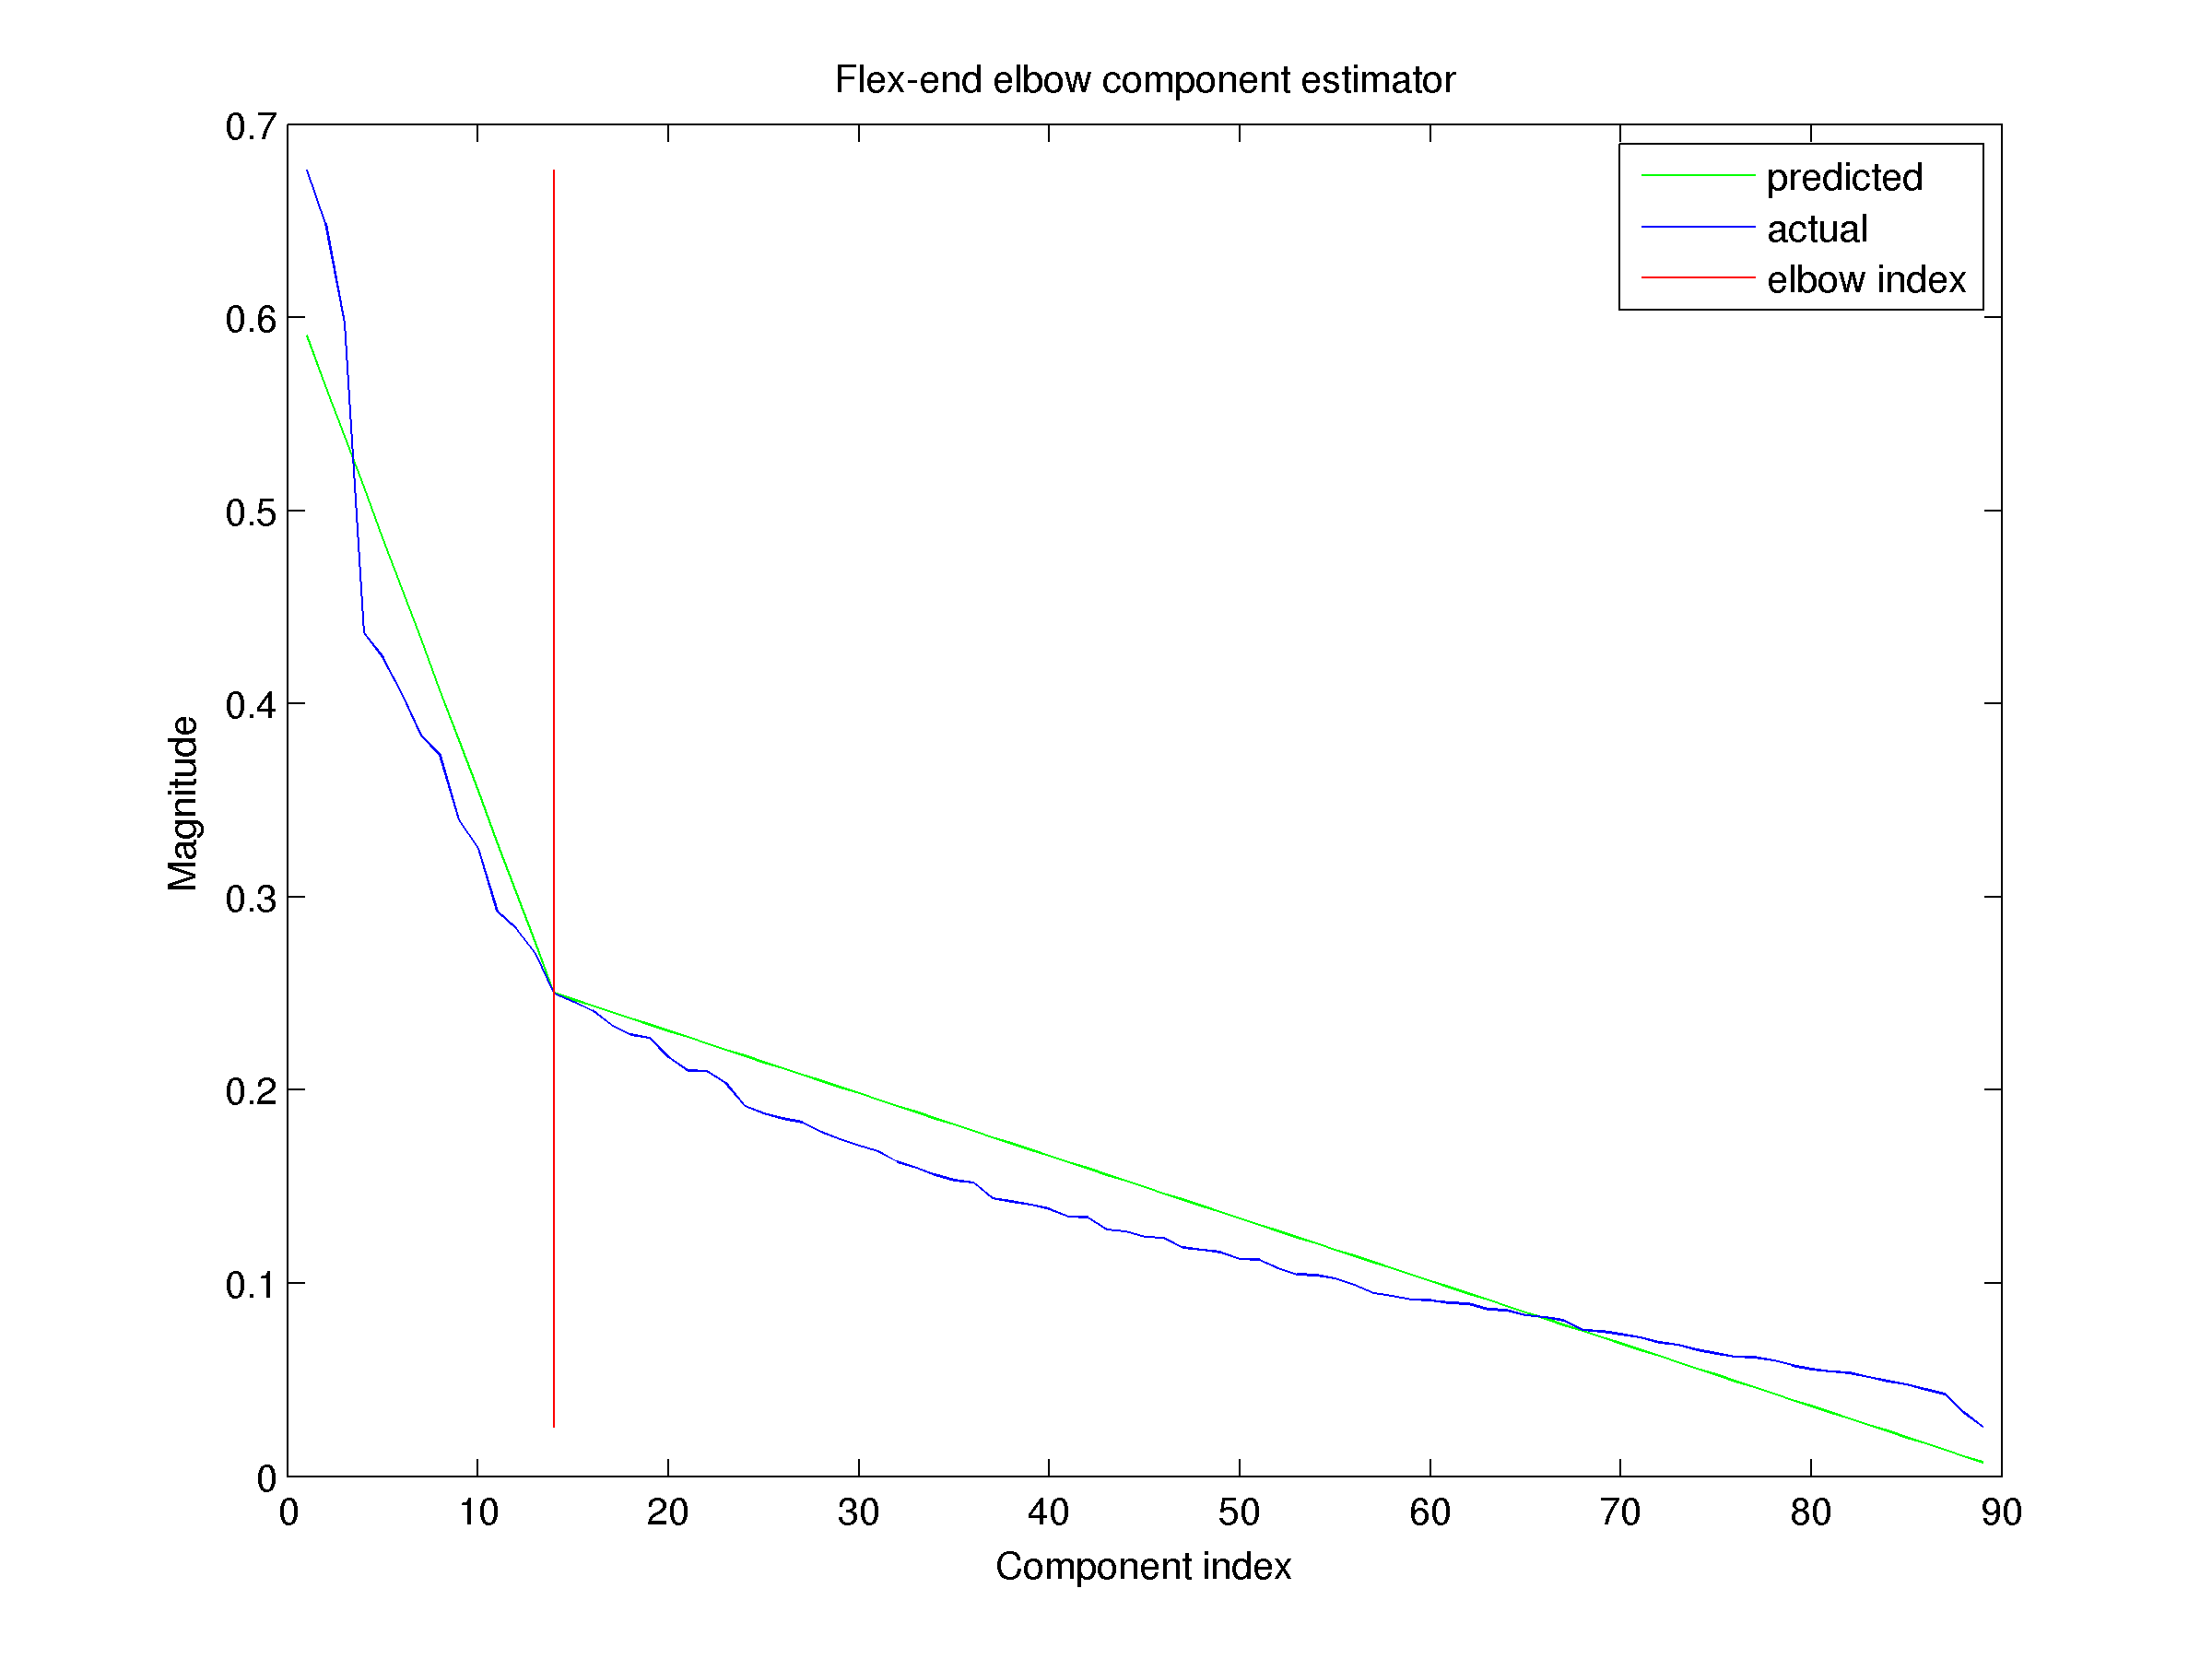
\includegraphics[width=0.9\linewidth]{100words-adj-800dim-lowercase-wmt-model-original-flex_end_elbow}
    \caption{Eigenvalues for each principal component of the 90 word vectors
    produced from the 101 word list.}
    \label{fig:101wordsunnormalizedpcaeigenvalues}
\end{figure}

\todo{switch the lambda plots in the results section to something properly labeled and scaled for easy comparison and without the elbow drawing}

\todo{make summary table plots into table rather than longtable environments so that they don't split across pages}

Table \ref{tab:101wordsRankingsUnnormalizedPCA} gives the highest and lowest
ranking words on the first 4 principal components of the unnormalized 90 word 
vectors. A more complete list can be found in Appendix 
\ref{app:rankedwordlists:101words:unnormalized}. The eigenvalues associated 
with each component are plotted in Figure 
\ref{fig:101wordsunnormalizedpcaeigenvalues}. The eigenvalue for a component is
proportional to the fraction of variance explained by that component.


\subsection{Normalized PCA}

\begin{longtable}[tbp]{| rllll |}
    \hline
      & \multicolumn{4}{c|}{\textbf{Component}} \\
    \textbf{Rank} & \textbf{1} & \textbf{2} & \textbf{3} & \textbf{4} \\
    \endhead
    \hline
    1 & irritable\_jj  & uncooperative\_jj  & negligent\_jj  & cold\_jj \\
    2 & uncooperative\_jj  & prompt\_jj  & uncooperative\_jj  & unreflective\_jj \\
    3 & self-pitying\_jj  & negligent\_jj  & imperturbable\_jj  & neat\_jj \\
    4 & extroverted\_jj  & systematic\_jj  & selfish\_jj  & self-pitying\_jj \\
    5 & unintelligent\_jj  & distrustful\_jj  & careless\_jj  & deep\_jj \\
    6 & talkative\_jj  & inconsistent\_jj  & prompt\_jj  & warm\_jj \\
    7 & rude\_jj  & insecure\_jj  & unreflective\_jj  & shallow\_jj \\
    \hline
    84 & steady\_jj  & uncharitable\_jj  & energetic\_jj  & thorough\_jj \\
    85 & simple\_jj  & talkative\_jj  & extroverted\_jj  & cooperative\_jj \\
    86 & systematic\_jj  & extroverted\_jj  & talkative\_jj  & talkative\_jj \\
    87 & innovative\_jj  & introspective\_jj  & pleasant\_jj  & kind\_jj \\
    88 & efficient\_jj  & energetic\_jj  & kind\_jj  & negligent\_jj \\
    89 & prompt\_jj  & considerate\_jj  & warm\_jj  & uncooperative\_jj \\
    90 & thorough\_jj  & imperturbable\_jj  & considerate\_jj  & considerate\_jj \\
    \hline
    \caption{The highest and lowest ranking words on the first 4 components 
    derived from normalized PCA of the 90 word vectors.}
    \label{tab:101wordsRankingsNormalizedPCA}
\end{longtable}


\begin{figure}[!tbp]
    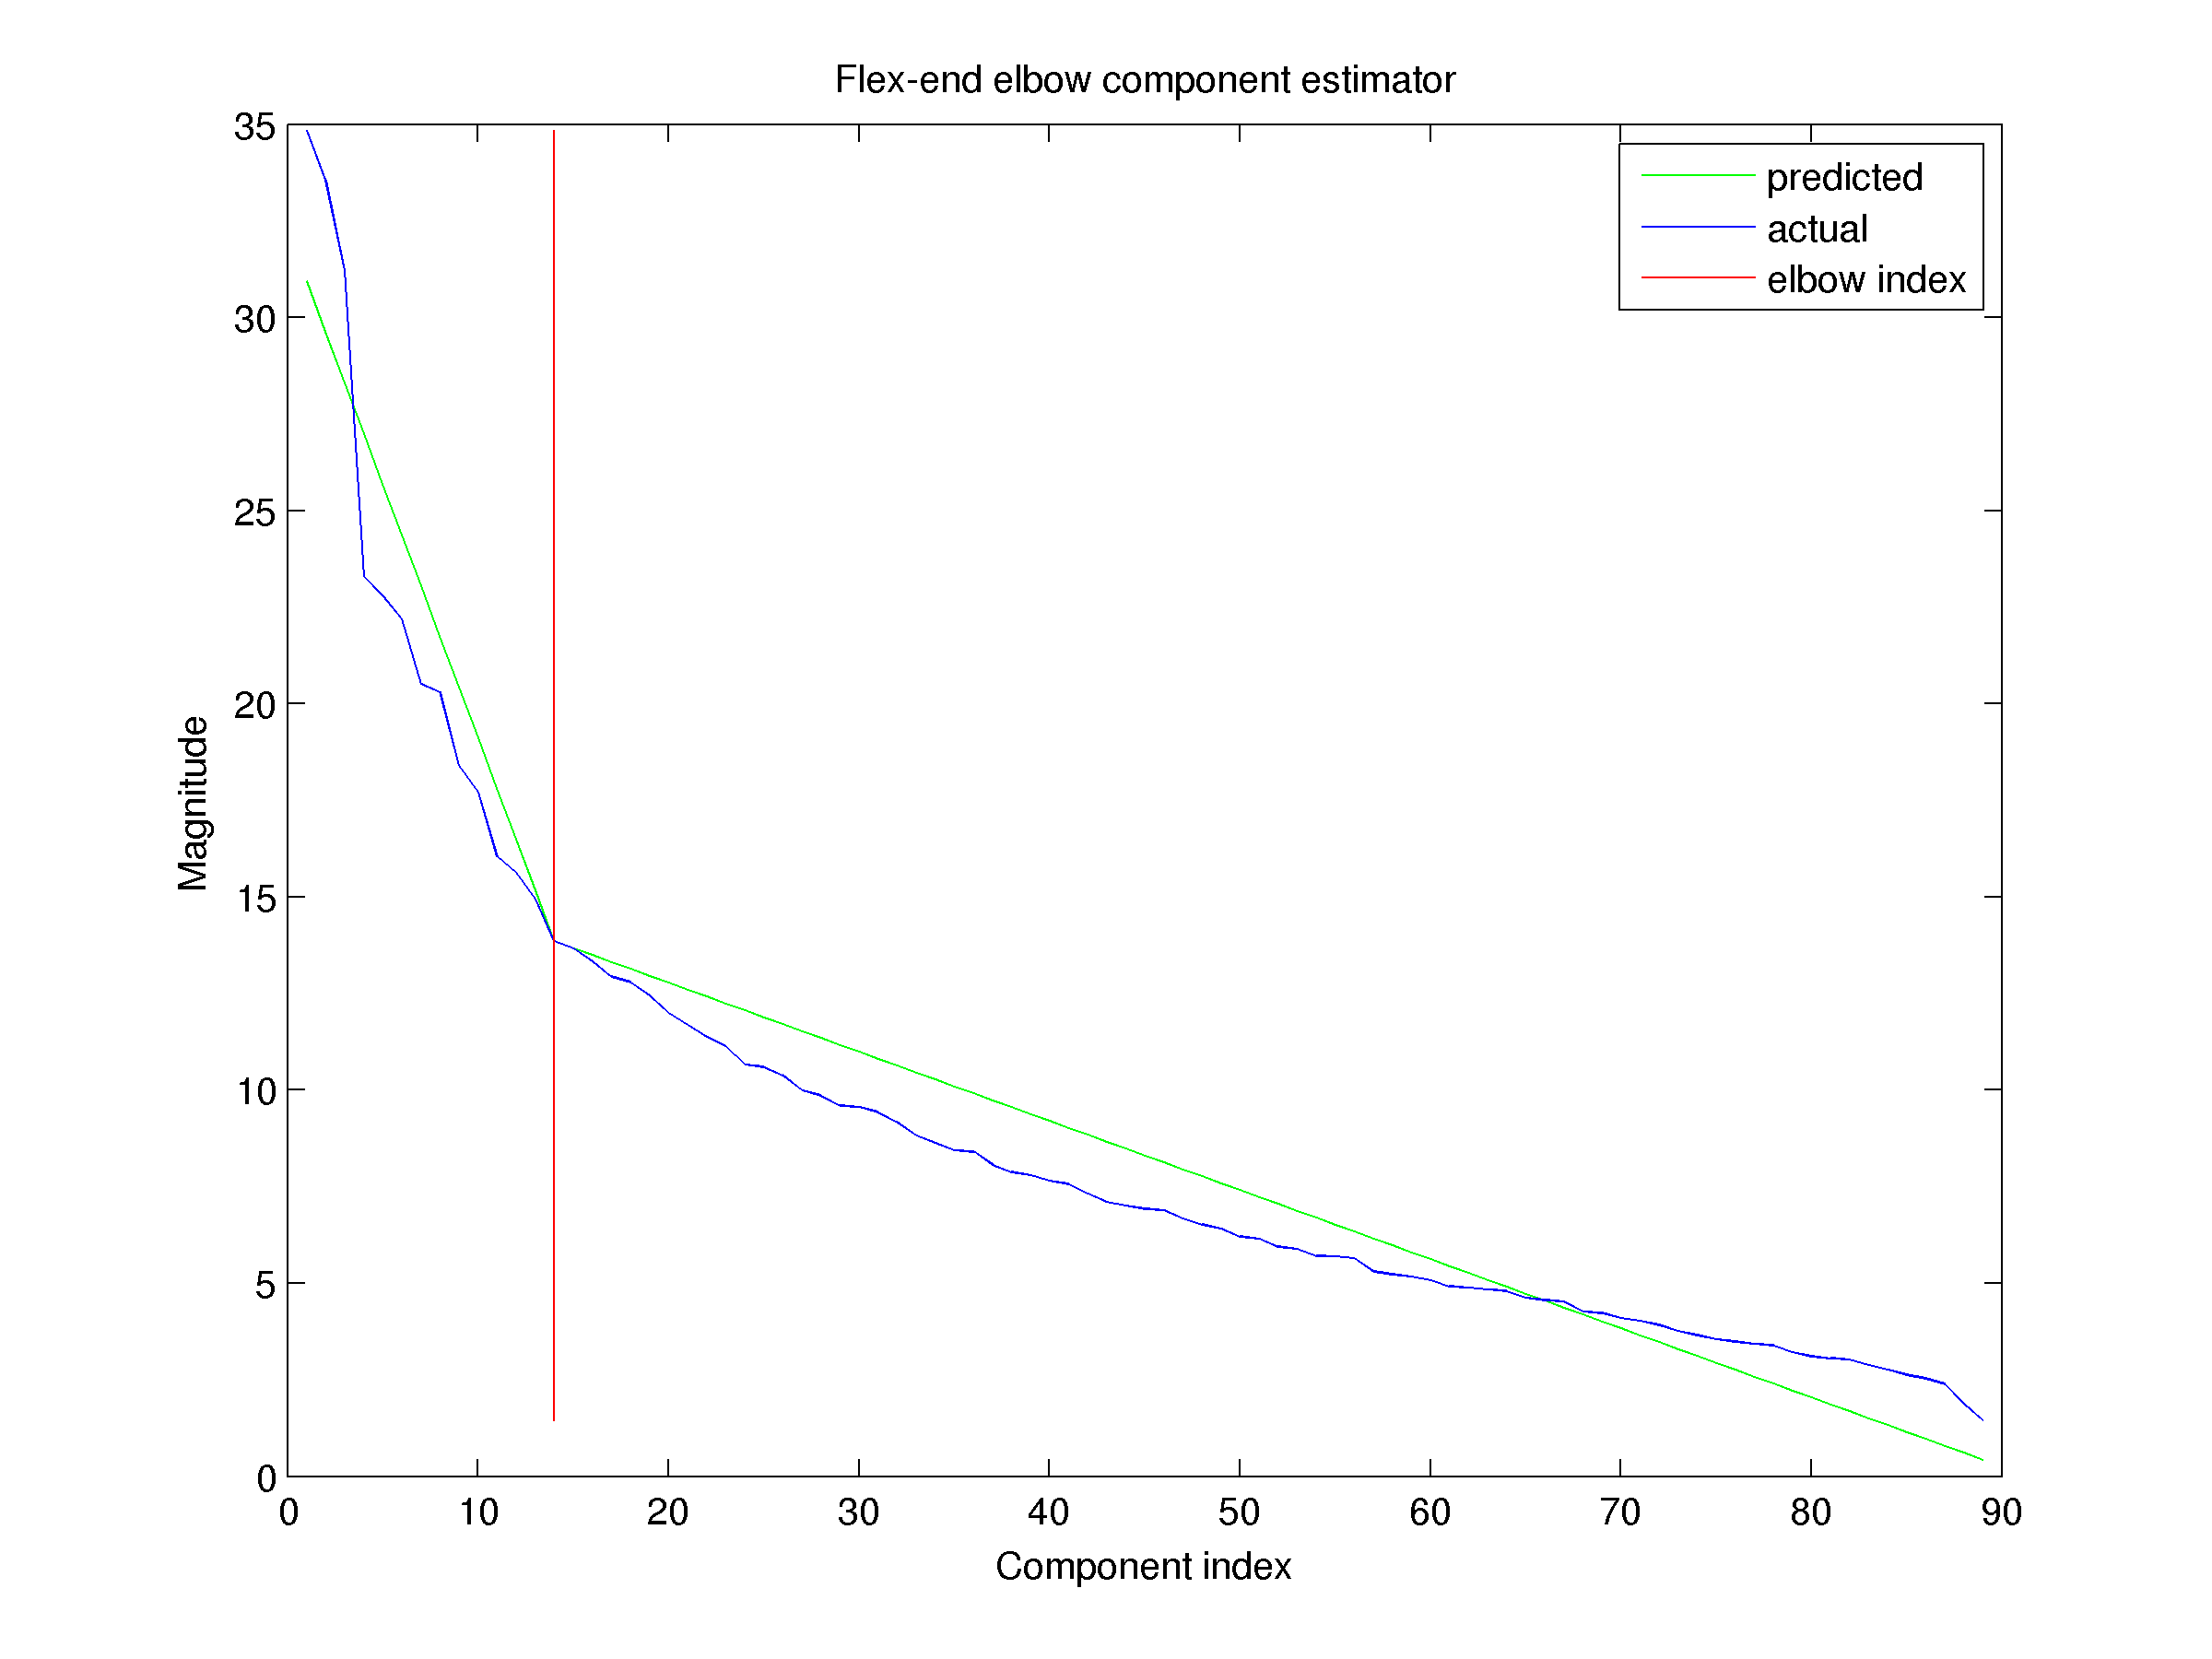
\includegraphics[width=0.9\linewidth]{100words-adj-800dim-lowercase-wmt-model-zscore-transformed-flex_end_elbow}
    \caption{Eigenvalues for each principal component of the 90 word vectors
    produced from the 101 word list after transforming to z-scores.}
    \label{fig:101wordsnormalizedpcaeigenvalues}
\end{figure}

Table \ref{tab:101wordsRankingsNormalizedPCA} gives the highest and lowest
ranking words on the first 4 principal components of the normalized 90 word 
vectors. A more complete list can be found in Appendix 
\ref{app:rankedwordlists:101words:normalized}. The eigenvalues associated 
with each component are plotted in Figure 
\ref{fig:101wordsnormalizedpcaeigenvalues}. The eigenvalue for a component is
proportional to the fraction of variance explained by that component.


\subsection{MDS}

\begin{longtable}[!htbp]{| rllll |}
    \hline
      & \multicolumn{4}{c|}{\textbf{Component}} \\
    \textbf{Rank} & \textbf{1} & \textbf{2} & \textbf{3} & \textbf{4} \\
    \endhead
    \hline
    1 & envious\_jj  & energetic\_jj  & imaginative\_jj  & active\_jj \\
    2 & jealous\_jj  & considerate\_jj  & artistic\_jj  & cooperative\_jj \\
    3 & self-pitying\_jj  & introspective\_jj  & innovative\_jj  & efficient\_jj \\
    4 & unkind\_jj  & pleasant\_jj  & unreflective\_jj  & sympathetic\_jj \\
    5 & bashful\_jj  & creative\_jj  & unadventurous\_jj  & assertive\_jj \\
    6 & fretful\_jj  & imaginative\_jj  & unimaginative\_jj  & unsympathetic\_jj \\
    7 & uncharitable\_jj  & extroverted\_jj  & creative\_jj  & distrustful\_jj \\
    \hline
    84 & systematic\_jj  & uncooperative\_jj  & careful\_jj  & bright\_jj \\
    85 & thorough\_jj  & inefficient\_jj  & quiet\_jj  & steady\_jj \\
    86 & efficient\_jj  & systematic\_jj  & warm\_jj  & shallow\_jj \\
    87 & complex\_jj  & sloppy\_jj  & cold\_jj  & warm\_jj \\
    88 & simple\_jj  & inconsistent\_jj  & fearful\_jj  & neat\_jj \\
    89 & practical\_jj  & unsystematic\_jj  & anxious\_jj  & deep\_jj \\
    90 & innovative\_jj  & negligent\_jj  & nervous\_jj  & cold\_jj \\
    \hline
    \caption{\todo{need to caption the table for 100words-adj-800dim-lowercase-wmt-model-mds-transformed-summary-table.tex} } \\
\end{longtable}


\begin{figure}[!tbp]
    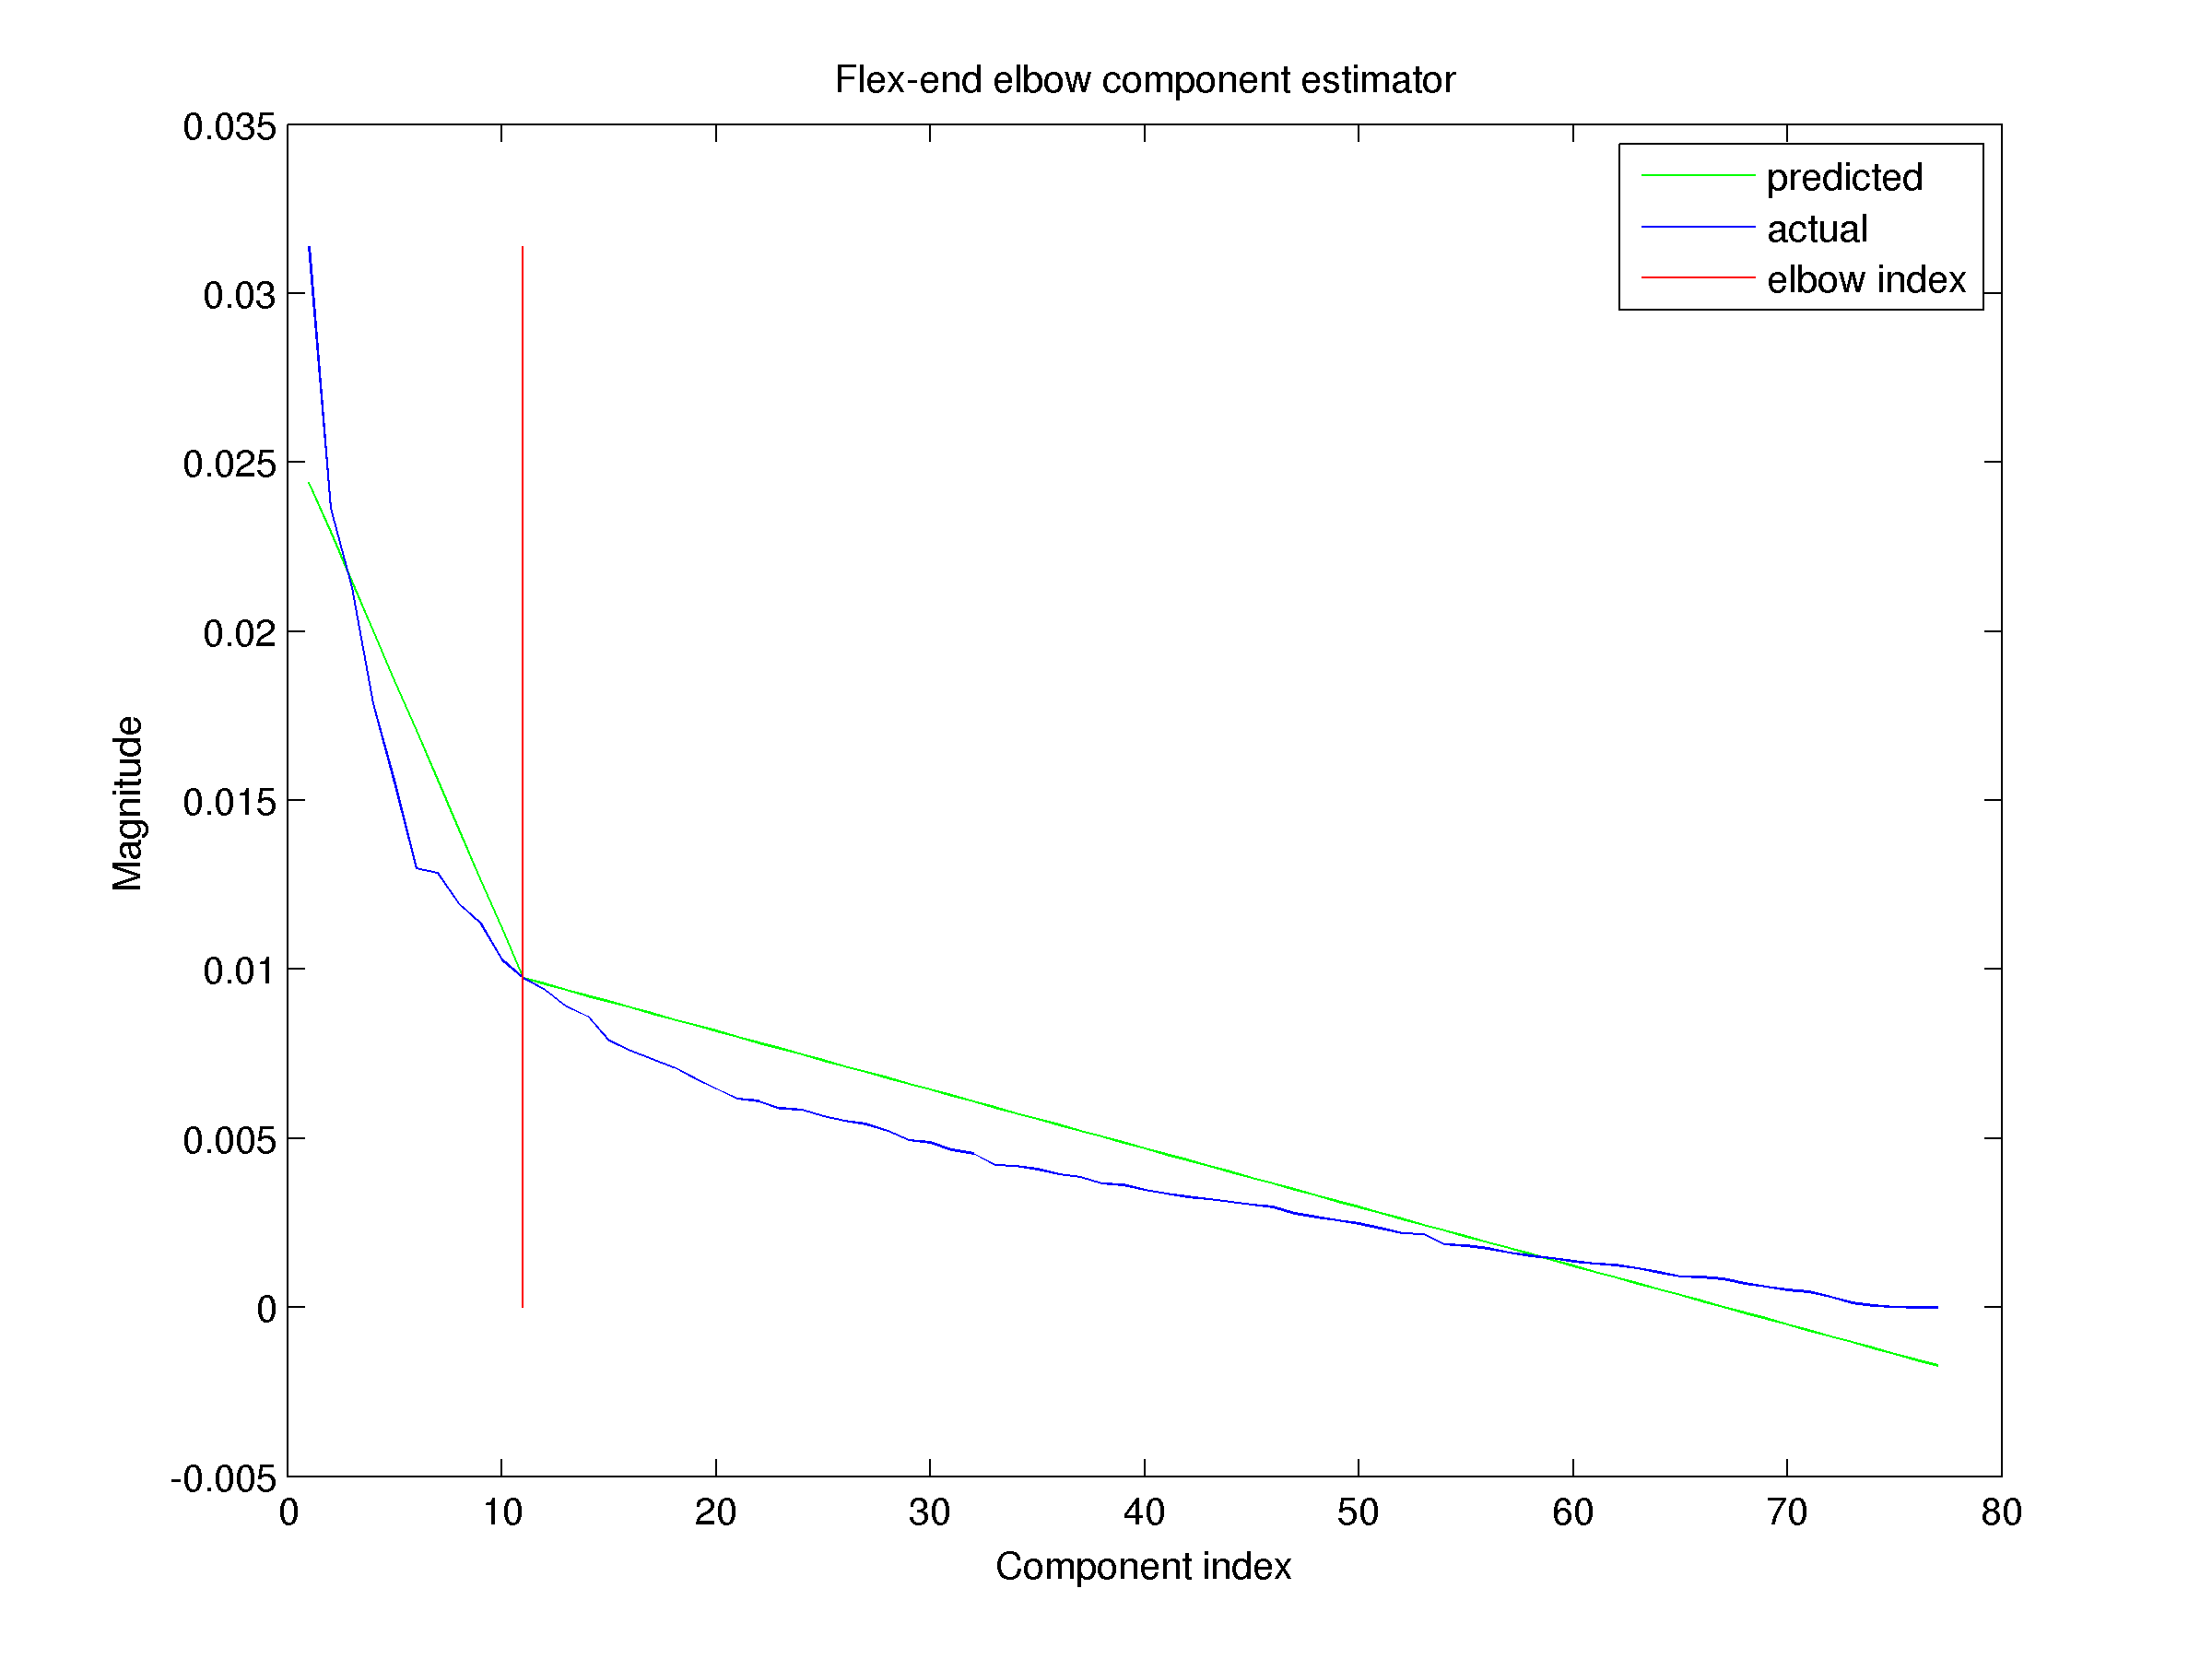
\includegraphics[width=0.9\linewidth]{100words-adj-800dim-lowercase-wmt-model-mds-transformed-flex_end_elbow}
    \caption{Eigenvalues for each principal component of the 90 word vectors
    produced from the 101 word list after multidimensional scaling.}
    \label{fig:101wordsmdseigenvalues}
\end{figure}

Table \ref{tab:101wordsRankingsMDS} gives the highest and lowest
ranking words on the first 4 principal components of the 90 word 
vectors after MDS. A more complete list can be found in Appendix 
\ref{app:rankedwordlists:101words:mds}. The eigenvalues associated 
with each component are plotted in Figure 
\ref{fig:101wordsmdseigenvalues}. The eigenvalue for a component is
proportional to the fraction of variance explained by that component.


\section{438 word set}

The 438 word set contained both adjectives and non-adjectives. Of these, 421 
were present in sufficient frequency to generate vectors within the memory 
constraints of the hardware on which I ran the skip-gram model. These words are 
listed in table \ref{tab:438wordsthatbecamevectors}. This produced 421 vectors 
on which further processing was performed. The adjectives carry the \_jj suffix 
from the Penn Treebank \todo{ref cite penn treebank} and the non-adjectives have 
no suffix.

\begin{longtable}[!htbp]{| llll |}
    \hline
    \endhead
   absent-minded\_jj & abusive\_jj & accommodating\_jj & active\_jj \\
   adaptable\_jj & adventurous\_jj & affectionate\_jj & agreeable\_jj \\
   aimless\_jj & aimlessness & aloofness & ambition \\
   ambitious\_jj & amiability & amiable\_jj & analytical\_jj \\
   animation & antagonistic\_jj & anxious\_jj & argumentative\_jj \\
   artistic\_jj & assertion & assertive\_jj & assured\_jj \\
   autonomous\_jj & bashful\_jj & belligerence & benevolent\_jj \\
   bigoted\_jj & bitter\_jj & boastful\_jj & bossiness \\
   bossy\_jj & brave\_jj & bright\_jj & bullheaded\_jj \\
   callousness & candor & carefree\_jj & careful\_jj \\
   careless\_jj & casual\_jj & caustic\_jj & caution \\
   cautious\_jj & charitable\_jj & cheerful\_jj & cold\_jj \\
   combative\_jj & communicative\_jj & compassionate\_jj & complex\_jj \\
   conceit & conceited\_jj & concise\_jj & condescending\_jj \\
   confident\_jj & considerate\_jj & consistent\_jj & contemplative\_jj \\
   conventional\_jj & conventionality & cooperation & cooperative\_jj \\
   cordial\_jj & cosmopolitan\_jj & courage & courageous\_jj \\
   courteous\_jj & courtesy & crabby\_jj & crafty\_jj \\
   cranky\_jj & creative\_jj & creativity & cruel\_jj \\
   cruelty & cultured\_jj & cunning & cunning\_jj \\
   curiosity & curious\_jj & curt\_jj & cynical\_jj \\
   daring & daring\_jj & deceit & deceitful\_jj \\
   decisive\_jj & decisiveness & deep\_jj & defensive\_jj \\
   deliberate\_jj & demanding\_jj & demonstrative\_jj & dependability \\
   dependable\_jj & depth & detached\_jj & devious\_jj \\
   dignified\_jj & dignity & diplomatic\_jj & direct\_jj \\
   dishonest\_jj & disorganization & disrespectful\_jj & distrust \\
   distrustful\_jj & docile\_jj & dominant\_jj & down-to-earth\_jj \\
   dull\_jj & earthiness & earthy\_jj & easygoing\_jj \\
   economical\_jj & efficiency & efficient\_jj & egocentric\_jj \\
   egotistical\_jj & emotional\_jj & emotionality & empathy \\
   energetic\_jj & enterprising\_jj & enthusiastic\_jj & envious\_jj \\
   envy & erratic\_jj & ethical\_jj & exacting\_jj \\
   excitable\_jj & exhibitionistic\_jj & explosive\_jj & expressive\_jj \\
   expressiveness & extravagant\_jj & extroverted\_jj & fastidious\_jj \\
   fear & fearful\_jj & firm\_jj & flamboyant\_jj \\
   flexibility & flexible\_jj & flippant\_jj & folksy\_jj \\
   foolhardy\_jj & forceful\_jj & foresighted\_jj & forgetful\_jj \\
   forgetfulness & formal\_jj & frank\_jj & fretful\_jj \\
   friendly\_jj & frivolity & frivolous\_jj & generosity \\
   generous\_jj & genial\_jj & greedy\_jj & gregarious\_jj \\
   gregariousness & gruff\_jj & grumpy\_jj & gullibility \\
   gullible\_jj & haphazard\_jj & happy-go-lucky\_jj & harsh\_jj \\
   helpful\_jj & homespun\_jj & honest\_jj & humble\_jj \\
   humor & humorous\_jj & ignorant\_jj & imaginative\_jj \\
   impersonal\_jj & impetuous\_jj & impolite\_jj & impractical\_jj \\
   impudent\_jj & inconsiderate\_jj & inconsistency & inconsistent\_jj \\
   indecisive\_jj & indecisiveness & independence & independent\_jj \\
   individualistic\_jj & industrious\_jj & inefficient\_jj & informal\_jj \\
   inhibition & innovative\_jj & inquisitive\_jj & insecure\_jj \\
   insecurity & insensitive\_jj & insight & insightful\_jj \\
   instability & intellectual\_jj & intellectuality & intelligence \\
   intelligent\_jj & introspective\_jj & intrusive\_jj & intrusiveness \\
   inventive\_jj & irritability & irritable\_jj & jealous\_jj \\
   jovial\_jj & joyless\_jj & kind\_jj & lazy\_jj \\
   leniency & lenient\_jj & lethargic\_jj & lethargy \\
   logic & logical\_jj & manipulative\_jj & mannerly\_jj \\
   meddlesome\_jj & meditative\_jj & melancholic\_jj & merry\_jj \\
   meticulous\_jj & mischievous\_jj & miserly\_jj & modest\_jj \\
   modesty & moody\_jj & moral\_jj & morality \\
   morose\_jj & natural\_jj & naturalness & naïve\_jj \\
   negligence & negligent\_jj & nervous\_jj & nonconforming\_jj \\
   nonconformity & nosey\_jj & obliging\_jj & obstinate\_jj \\
   opportunistic\_jj & optimism & optimistic\_jj & orderly\_jj \\
   organization & organized\_jj & passionless\_jj & passive\_jj \\
   passivity & patient\_jj & peaceful\_jj & perceptive\_jj \\
   persistence & persistent\_jj & pessimism & pessimistic\_jj \\
   philosophical\_jj & placidity & playful\_jj & playfulness \\
   pleasant\_jj & polite\_jj & pomposity & pompous\_jj \\
   precise\_jj & precision & predictability & predictable\_jj \\
   prejudice & prejudiced\_jj & principled\_jj & prompt\_jj \\
   proud\_jj & punctual\_jj & punctuality & purposeful\_jj \\
   quarrelsome\_jj & quiet & quiet\_jj & rambunctious\_jj \\
   rash\_jj & reasonable\_jj & rebellious\_jj & reckless\_jj \\
   recklessness & refined\_jj & reliable\_jj & reserve \\
   reserved\_jj & respectful\_jj & responsible\_jj & restrained\_jj \\
   rude\_jj & rudeness & ruthless\_jj & scatterbrained\_jj \\
   scornful\_jj & secretive\_jj & self-critical\_jj & self-disciplined\_jj \\
   self-esteem & self-indulgent\_jj & self-pitying\_jj & selfish\_jj \\
   selfishness & selfless\_jj & sentimental\_jj & shallow\_jj \\
   shallowness & shy\_jj & shyness & silence \\
   silent\_jj & simple\_jj & sincere\_jj & skeptical\_jj \\
   sloppy\_jj & sloth & slothful\_jj & sluggish\_jj \\
   sly\_jj & smart\_jj & smug\_jj & snobbish\_jj \\
   sociable\_jj & somber\_jj & sophisticated\_jj & sophistication \\
   spirit & spirited\_jj & spontaneity & spontaneous\_jj \\
   steady\_jj & stinginess & stingy\_jj & straightforward\_jj \\
   stubborn\_jj & stubbornness & stupidity & submissive\_jj \\
   suggestible\_jj & surliness & surly\_jj & suspicious\_jj \\
   sympathetic\_jj & systematic\_jj & tactful\_jj & tactless\_jj \\
   talkative\_jj & talkativeness & temperamental\_jj & tempestuous\_jj \\
   tenacious\_jj & thorough\_jj & thoughtless\_jj & thoughtlessness \\
   thrift & thrifty\_jj & timid\_jj & touchy\_jj \\
   traditional\_jj & trustful\_jj & truthful\_jj & unadventurous\_jj \\
   unaggressive\_jj & unambitious\_jj & unassuming\_jj & unconventional\_jj \\
   uncritical\_jj & undemanding\_jj & undependable\_jj & underhanded\_jj \\
   understanding & understanding\_jj & unemotional\_jj & unexcitable\_jj \\
   unfriendliness & unfriendly\_jj & ungracious\_jj & unimaginative\_jj \\
   uninhibited\_jj & unintelligent\_jj & unkind\_jj & unobservant\_jj \\
   unpredictable\_jj & unreflective\_jj & unreliable\_jj & unrestrained\_jj \\
   unscrupulous\_jj & unsociable\_jj & unstable\_jj & unsympathetic\_jj \\
   unsystematic\_jj & vain\_jj & verbal\_jj & verbose\_jj \\
   vigorous\_jj & vindictive\_jj & vivacious\_jj & volatile\_jj \\
   volatility & warm\_jj & warmth & wishy-washy\_jj \\
   withdrawn\_jj & witty\_jj & wordy\_jj & worldly\_jj \\
   zestful\_jj & & &\\
    \hline
    \caption{The 421 words from the list of 438 for which vectors were generated.}
    \label{tab:438wordsthatbecamevectors}
\end{longtable}



\subsection{Unnormalized PCA}

\begin{longtable}[!htbp]{| rllll |}
    \hline
      & \multicolumn{4}{c|}{\textbf{Component}} \\
    \textbf{Rank} & \textbf{1} & \textbf{2} & \textbf{3} & \textbf{4} \\
    \endhead
    \hline
    1 & sociable\_jj  & callousness  & abusive\_jj  & sincere\_jj \\
    2 & vivacious\_jj  & selfishness  & inconsiderate\_jj  & considerate\_jj \\
    3 & considerate\_jj  & gullibility  & selfish\_jj  & dignity \\
    4 & easygoing\_jj  & stupidity  & disrespectful\_jj  & courage \\
    5 & witty\_jj  & recklessness  & insensitive\_jj  & selfless\_jj \\
    6 & affectionate\_jj  & rudeness  & ignorant\_jj  & honest\_jj \\
    7 & talkative\_jj  & deceit  & dishonest\_jj  & courageous\_jj \\
    \hline
    415 & caution  & optimistic\_jj  & warmth  & fretful\_jj \\
    416 & sluggish\_jj  & easygoing\_jj  & sophistication  & sluggish\_jj \\
    417 & intelligence  & efficient\_jj  & naturalness  & lethargic\_jj \\
    418 & cooperation  & reliable\_jj  & earthiness  & lethargy \\
    419 & volatility  & friendly\_jj  & expressiveness  & irritability \\
    420 & instability  & considerate\_jj  & spontaneity  & irritable\_jj \\
    421 & negligence  & sociable\_jj  & playfulness  & absent-minded\_jj \\
    \hline
    \caption{\todo{need to caption the table for 439words-adj-800dim-lowercase-wmt-model-original-summary-table.tex} } \\
\end{longtable}


\begin{figure}[!tbp]
    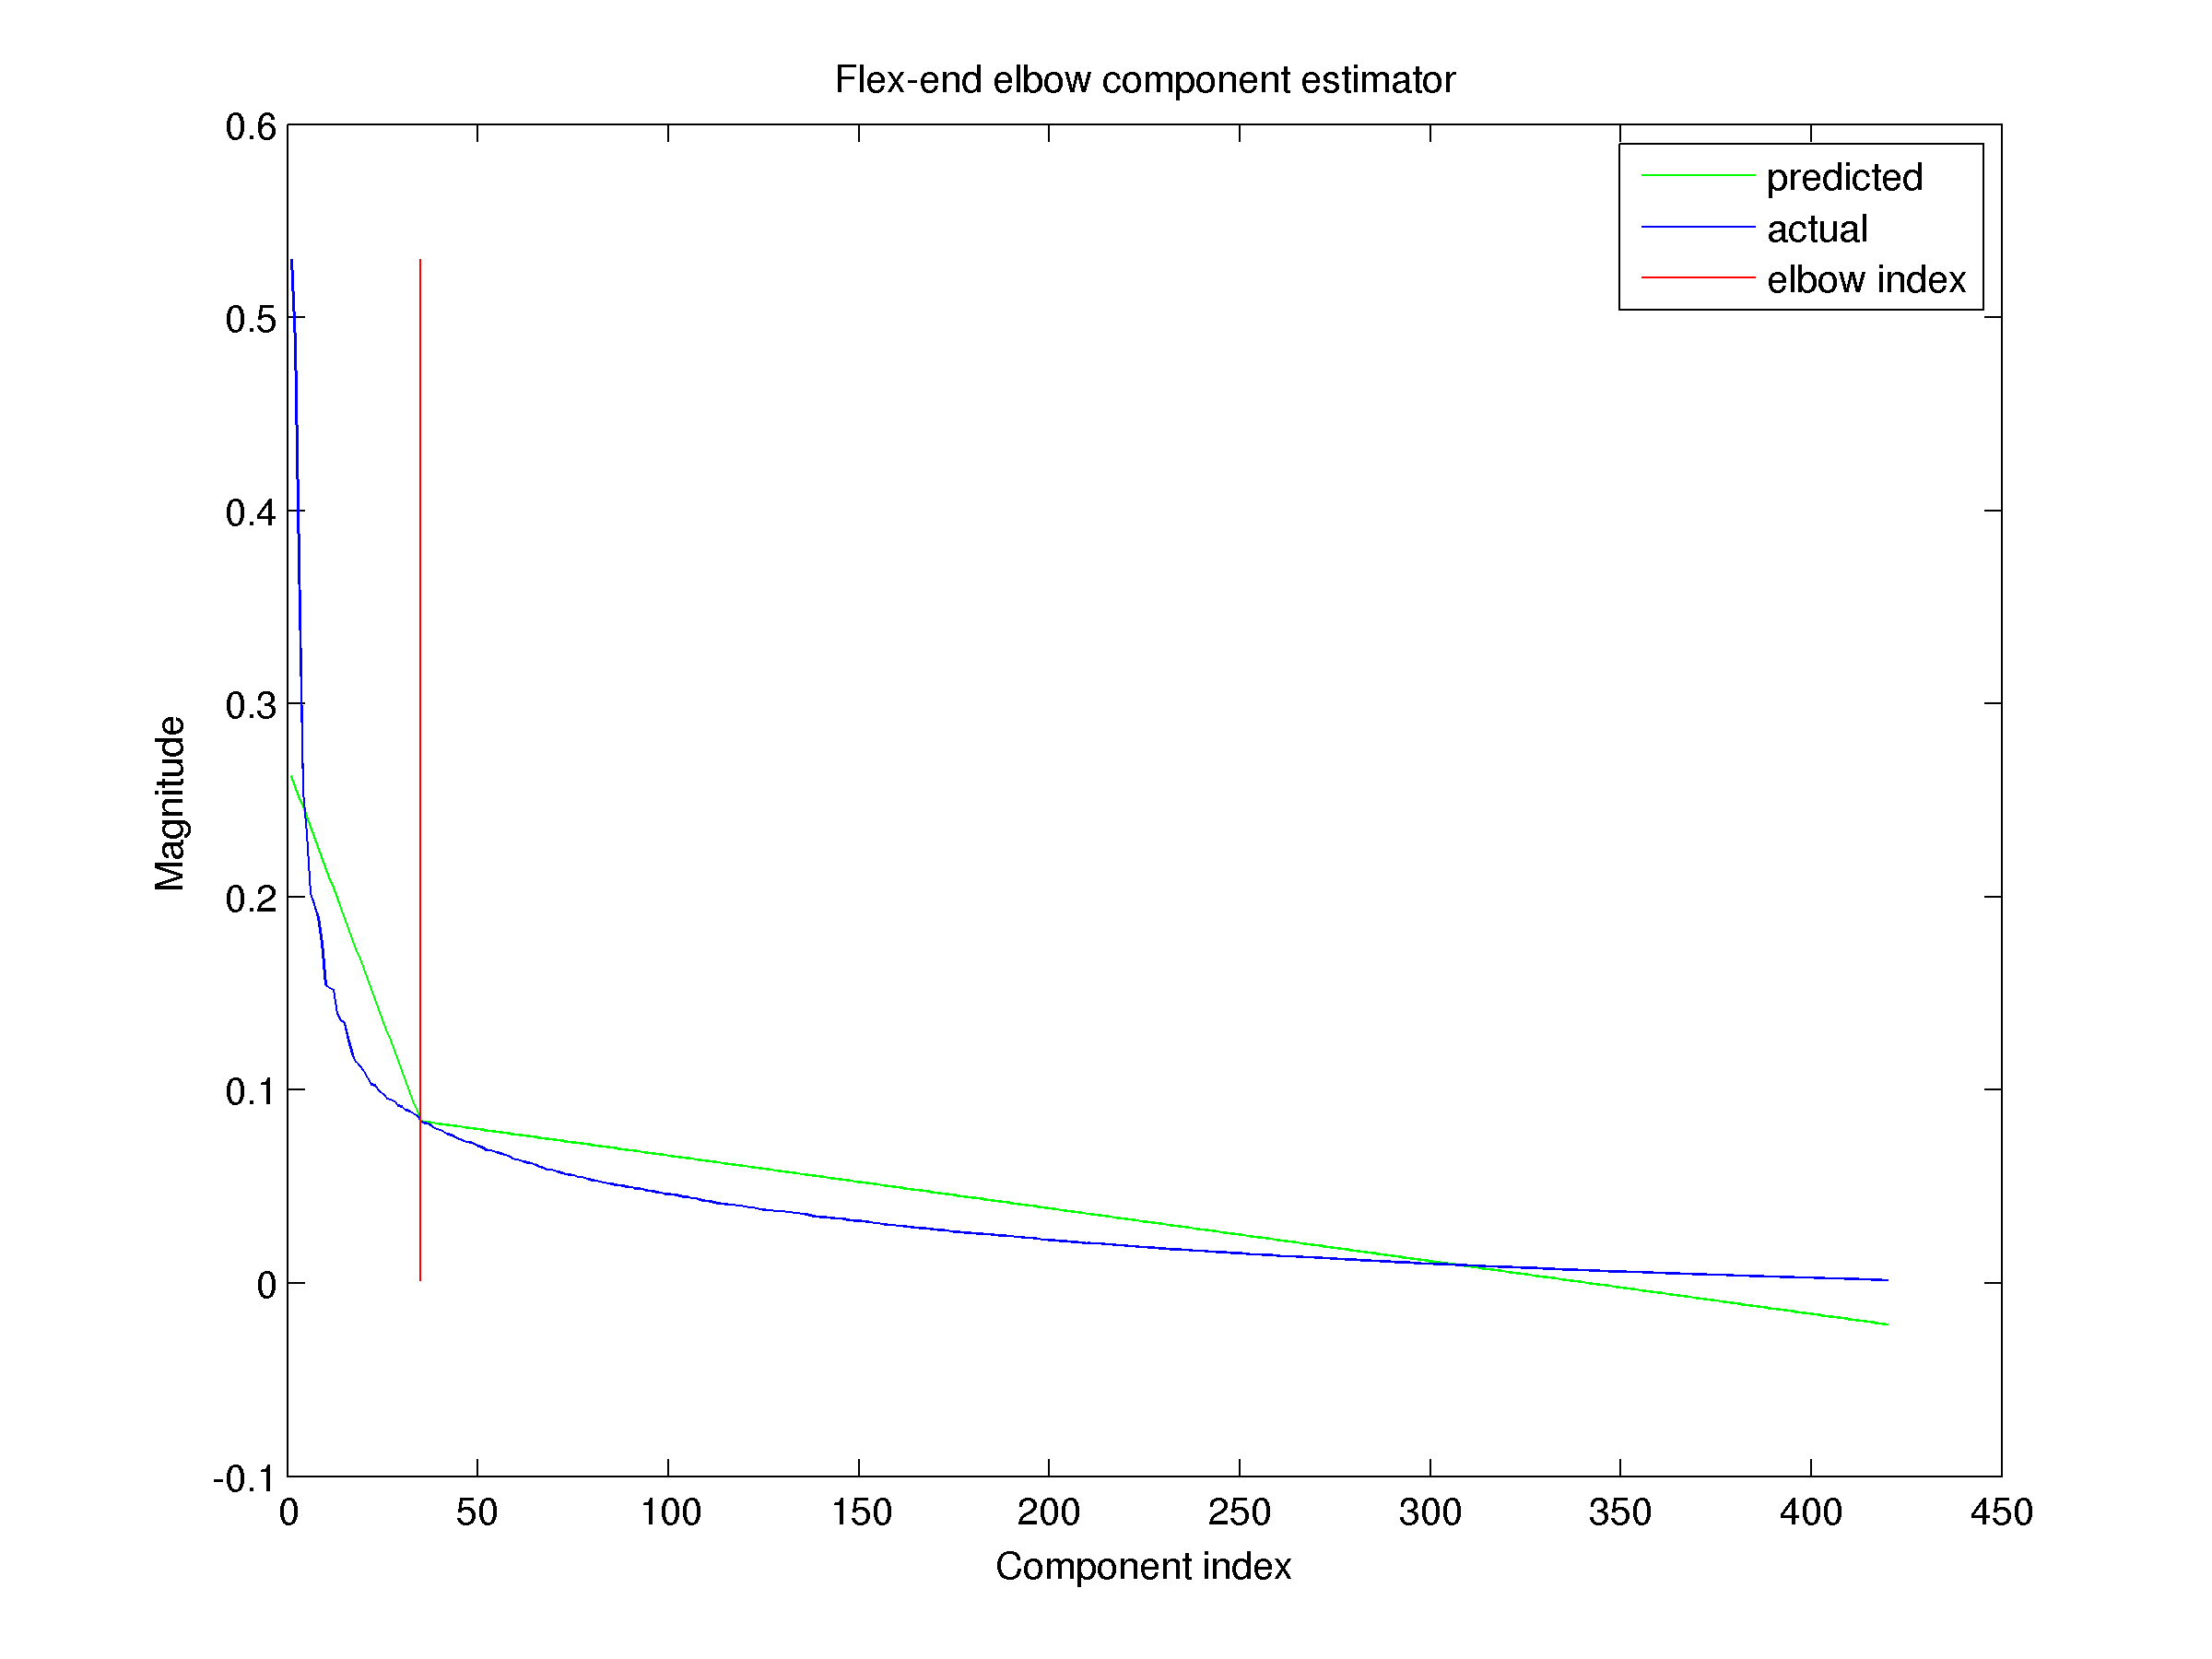
\includegraphics[width=0.9\linewidth]{439words-adj-800dim-lowercase-wmt-model-original-flex_end_elbow}
    \caption{Eigenvalues for each principal component of the 421 word vectors
    produced from the 438 word list.}
    \label{fig:438wordsunnormalizedpcaeigenvalues}
\end{figure}

Table \ref{tab:438wordsRankingsUnnormalizedPCA} gives the highest and lowest
ranking words on the first 4 principal components of the unnormalized 421 word 
vectors. A more complete list can be found in Appendix 
\ref{app:rankedwordlists:438words:unnormalized}.


\subsection{Normalized PCA}

\begin{longtable}[!htbp]{| rllll |}
    \hline
      & \multicolumn{4}{c|}{\textbf{Component}} \\
    \textbf{Rank} & \textbf{1} & \textbf{2} & \textbf{3} & \textbf{4} \\
    \endhead
    \hline
    1 & sociable\_jj  & callousness  & abusive\_jj  & sincere\_jj \\
    2 & vivacious\_jj  & selfishness  & inconsiderate\_jj  & considerate\_jj \\
    3 & considerate\_jj  & gullibility  & insensitive\_jj  & dignity \\
    4 & easygoing\_jj  & recklessness  & selfish\_jj  & courage \\
    5 & witty\_jj  & stupidity  & ignorant\_jj  & selfless\_jj \\
    6 & talkative\_jj  & rudeness  & disrespectful\_jj  & courageous\_jj \\
    7 & affectionate\_jj  & deceit  & dishonest\_jj  & honest\_jj \\
    \hline
    415 & caution  & dependable\_jj  & warmth  & erratic\_jj \\
    416 & sluggish\_jj  & easygoing\_jj  & earthiness  & lethargic\_jj \\
    417 & intelligence  & efficient\_jj  & sophistication  & sluggish\_jj \\
    418 & cooperation  & reliable\_jj  & naturalness  & lethargy \\
    419 & volatility  & friendly\_jj  & expressiveness  & irritability \\
    420 & instability  & considerate\_jj  & spontaneity  & irritable\_jj \\
    421 & negligence  & sociable\_jj  & playfulness  & absent-minded\_jj \\
    \hline
    \caption{\todo{need to caption the table for 439words-adj-800dim-lowercase-wmt-model-zscore-transformed-summary-table.tex} } \\
\end{longtable}


\begin{figure}[!tbp]
    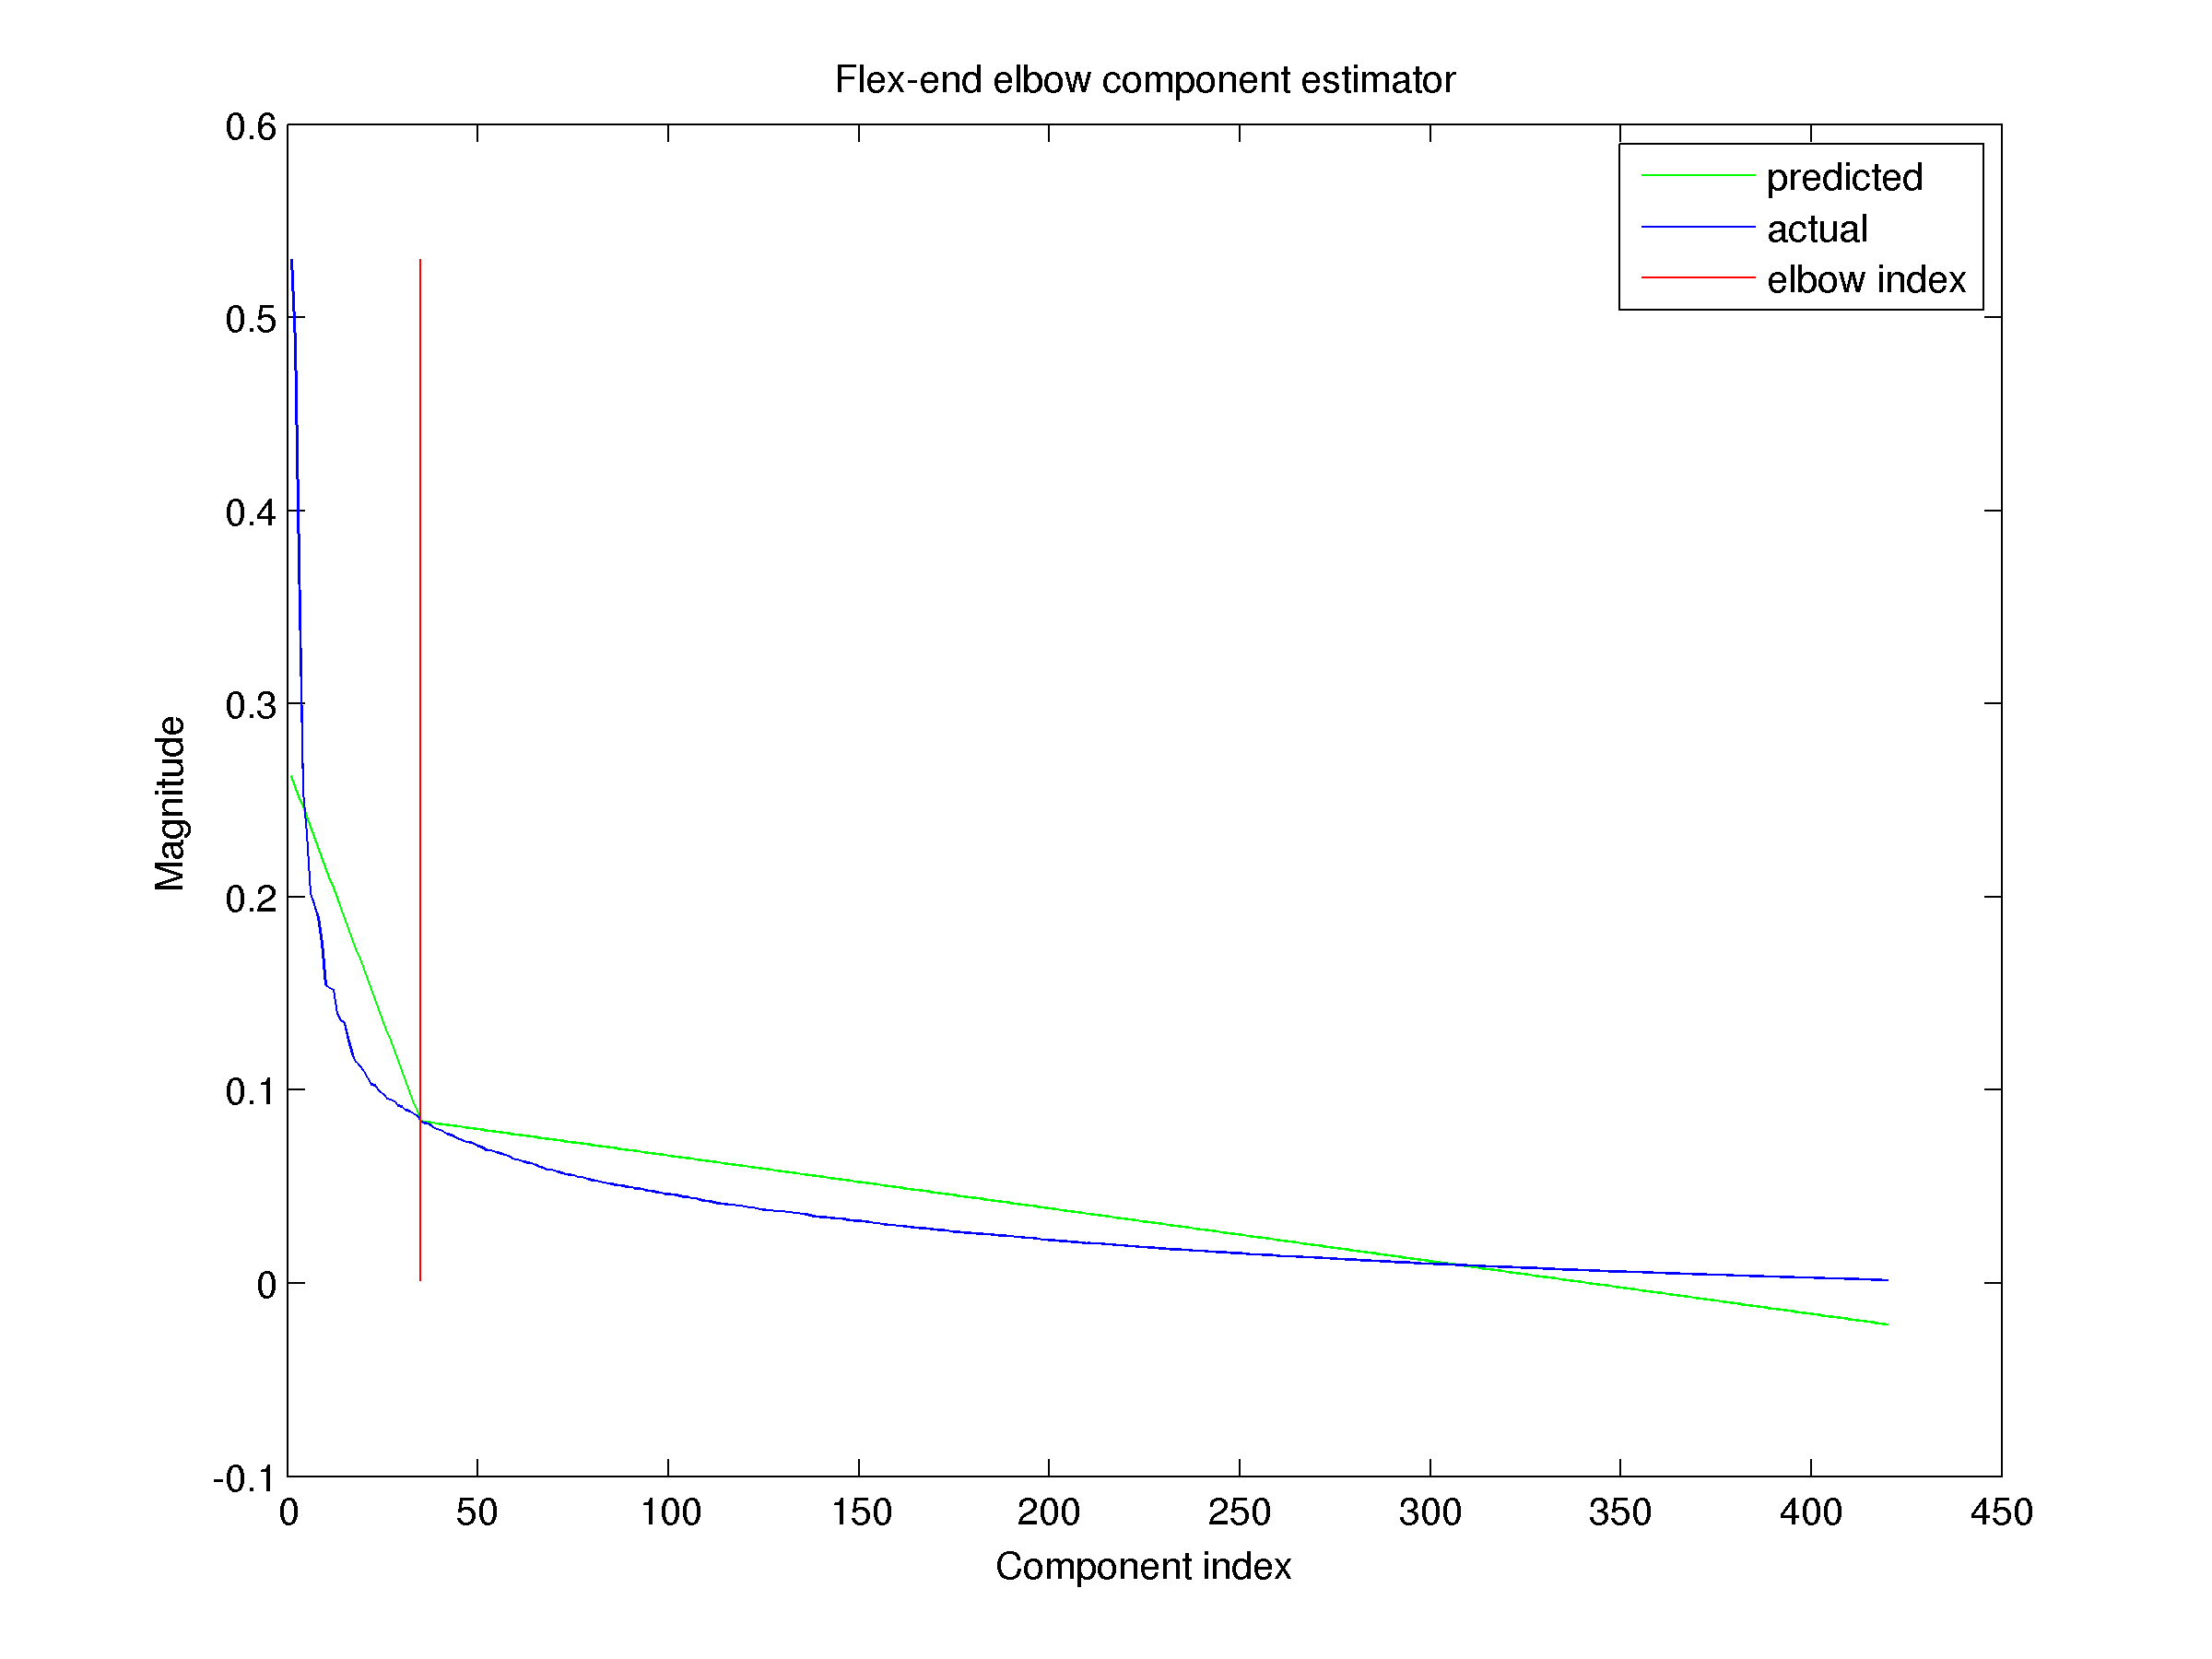
\includegraphics[width=0.9\linewidth]{439words-adj-800dim-lowercase-wmt-model-original-flex_end_elbow}
    \caption{Eigenvalues for each principal component of the 421 z-score 
    normalized word vectors produced from the 438 word list.}
    \label{fig:438wordsnormalizedpcaeigenvalues}
\end{figure}

Table \ref{tab:438wordsRankingsNormalizedPCA} gives the highest and lowest
ranking words on the first 4 principal components of the z-score normalized 421 
word vectors. A more complete list can be found in Appendix 
\ref{app:rankedwordlists:438words:normalized}.

\subsection{MDS}

\begin{longtable}[!htbp]{| rllll |}
    \hline
      & \multicolumn{4}{c|}{\textbf{Component}} \\
    \textbf{Rank} & \textbf{1} & \textbf{2} & \textbf{3} & \textbf{4} \\
    \endhead
    \hline
    1 & self-pitying\_jj  & sociable\_jj  & ignorant\_jj  & innovative\_jj \\
    2 & scatterbrained\_jj  & cheerful\_jj  & dishonest\_jj  & dishonest\_jj \\
    3 & pomposity  & vivacious\_jj  & insensitive\_jj  & intelligent\_jj \\
    4 & mischievous\_jj  & easygoing\_jj  & greedy\_jj  & ethical\_jj \\
    5 & sly\_jj  & considerate\_jj  & disrespectful\_jj  & imaginative\_jj \\
    6 & pompous\_jj  & enthusiastic\_jj  & bigoted\_jj  & truthful\_jj \\
    7 & snobbish\_jj  & dependable\_jj  & unfriendly\_jj  & honest\_jj \\
    \hline
    415 & volatile\_jj  & passivity  & spirit  & lethargy \\
    416 & reasonable\_jj  & deceit  & persistence  & irritable\_jj \\
    417 & flexibility  & recklessness  & playfulness  & cold\_jj \\
    418 & reliable\_jj  & gullibility  & spontaneity  & anxious\_jj \\
    419 & direct\_jj  & selfishness  & precision  & lethargic\_jj \\
    420 & cooperation  & callousness  & warmth  & sluggish\_jj \\
    421 & consistent\_jj  & stupidity  & creativity  & nervous\_jj \\
    \hline
    \caption{The highest and lowest ranking words on the first 4 components 
    derived from performaing MDS on the 421 word vectors.}
    \label{tab:438wordsRankingsMDS}
\end{longtable}


Table \ref{tab:438wordsRankingsMDS} gives the highest and lowest
ranking words on the first 4 principal components of the 421 word 
vectors after MDS. A more complete list can be found in Appendix 
\ref{app:rankedwordlists:438words:mds}.

\begin{figure}[!tbp]
    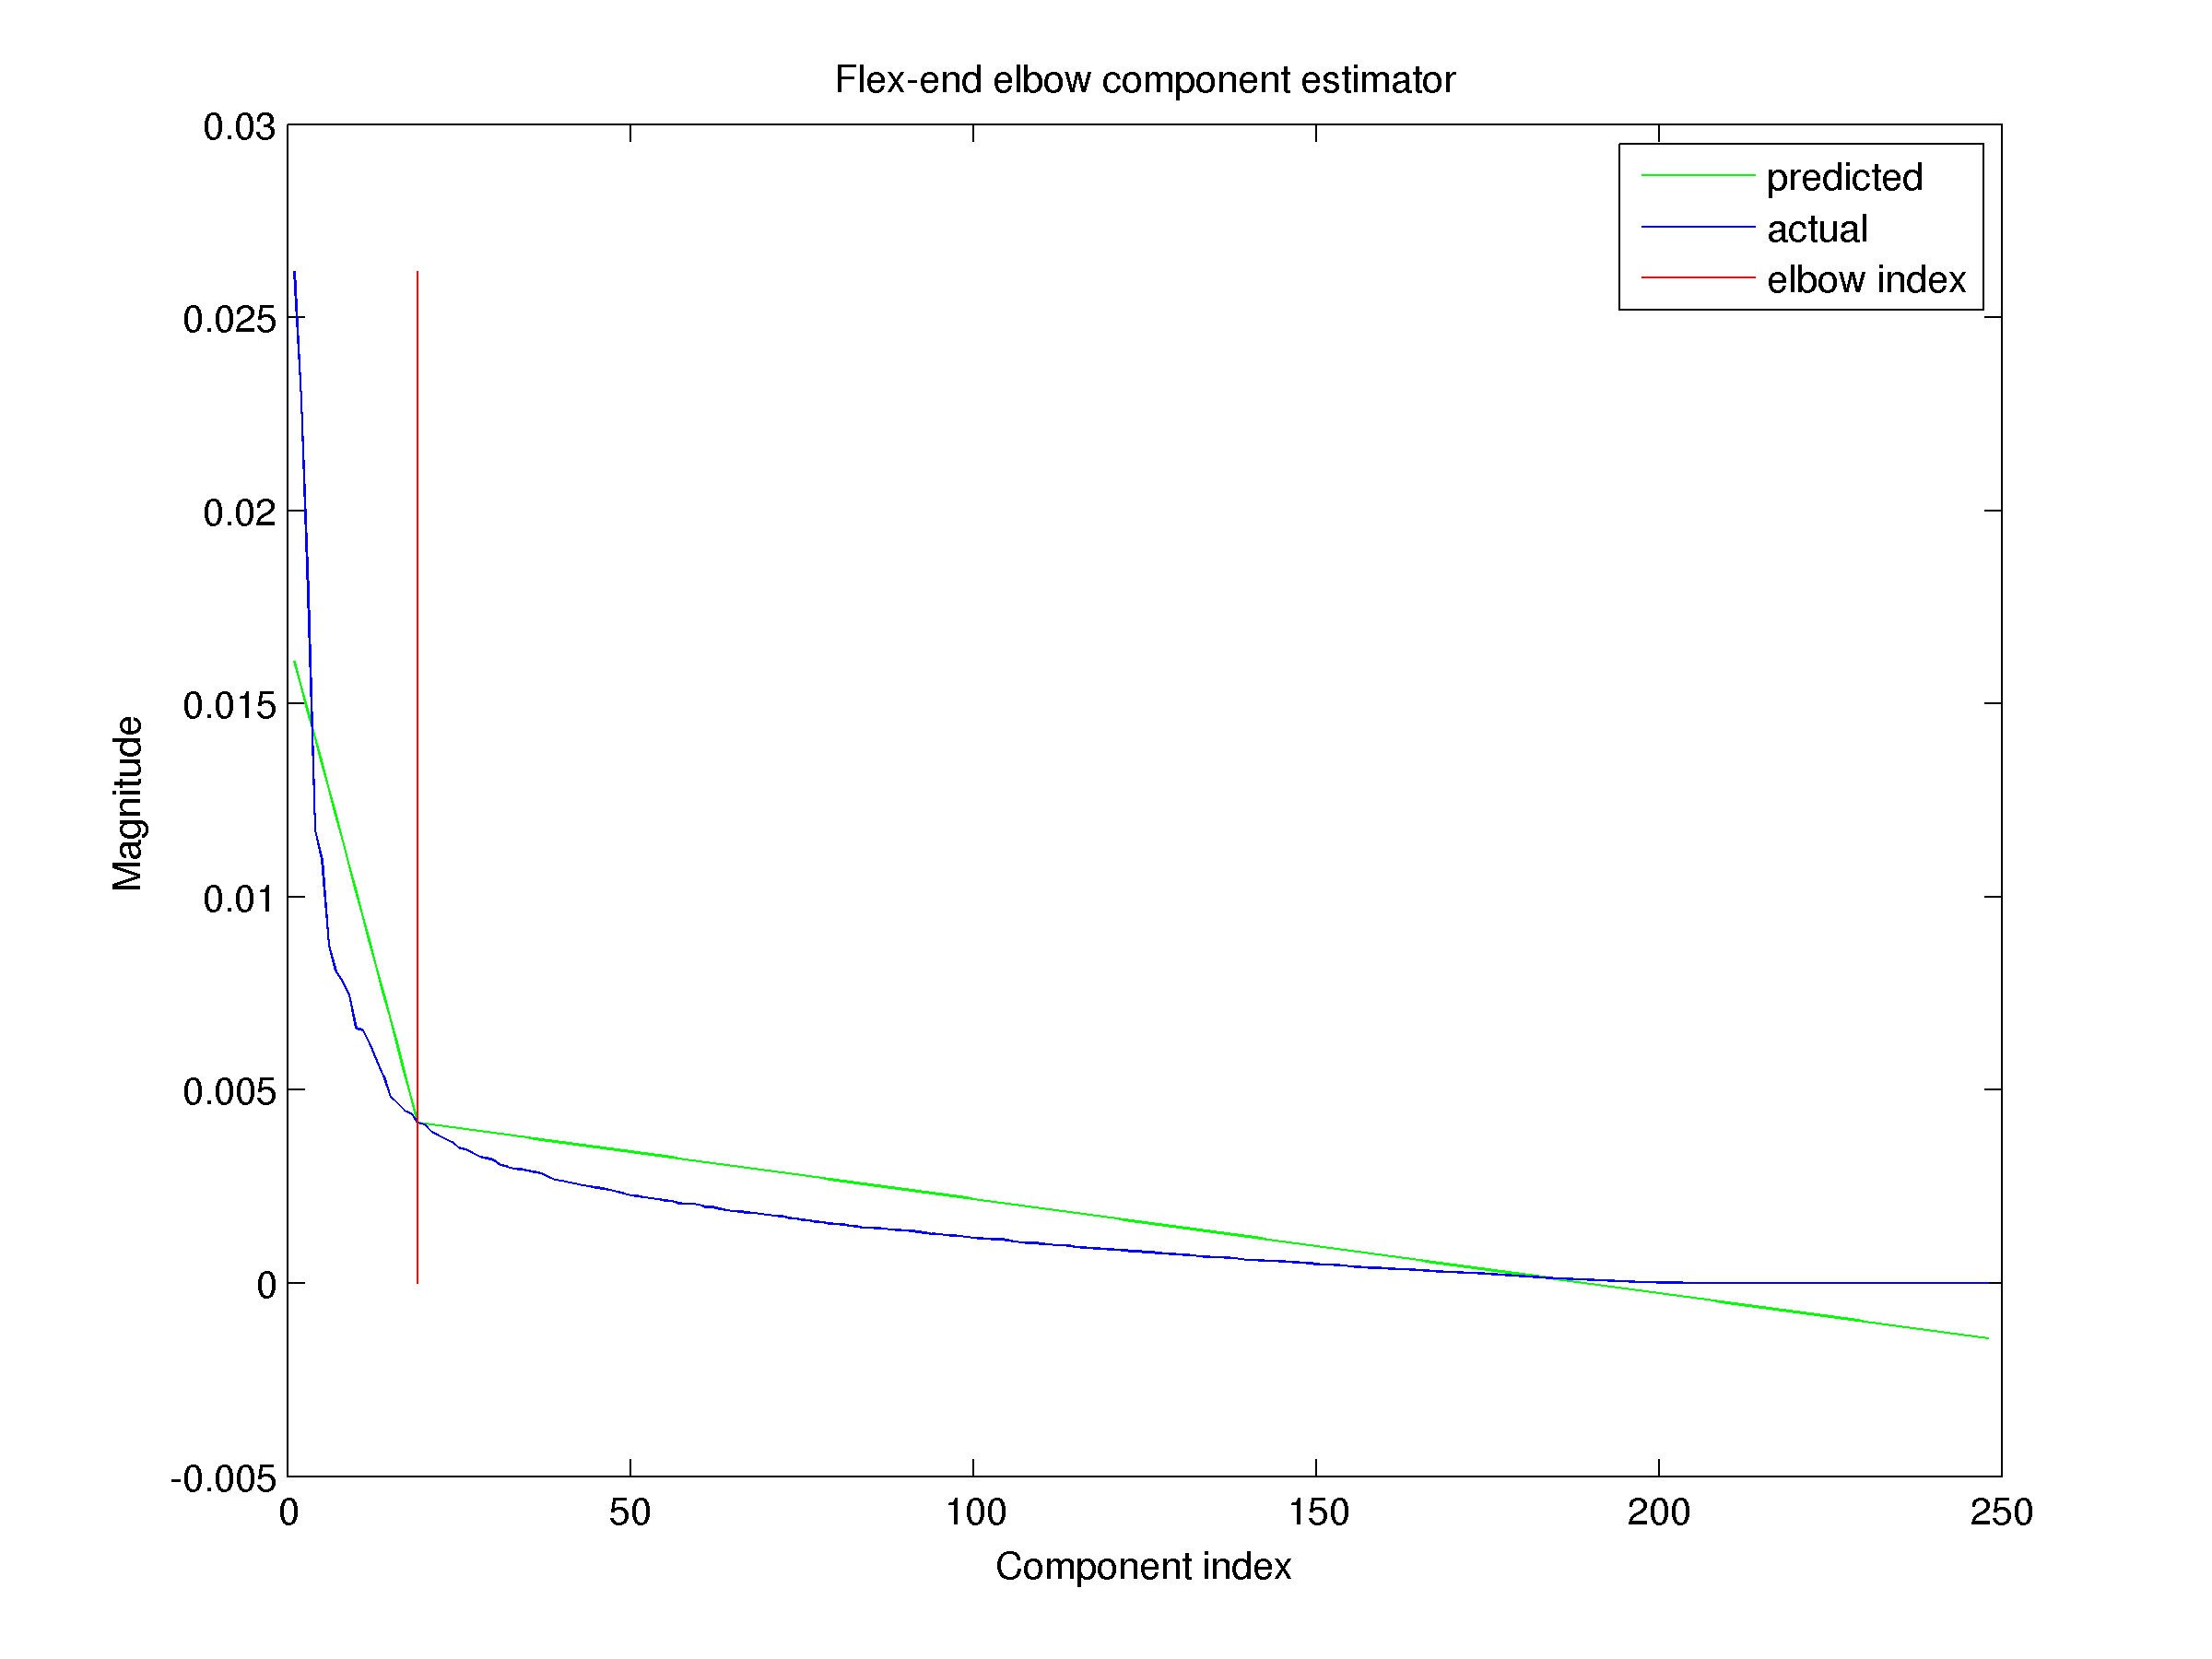
\includegraphics[width=0.9\linewidth]{439words-adj-800dim-lowercase-wmt-model-mds-transformed-flex_end_elbow}
    \caption{Eigenvalues for each principal component of the 421 word vectors
    produced from the 438 word list after multidimensional scaling.}
    \label{fig:438wordsmdseigenvalues}
\end{figure}


\section{101 and 438 word sets combined}

There were a few words in the 101 word list that were not also in the 438 word 
list. So, for completeness, I also ran the same analysis with the two lists 
combined. In the combined list, 430 words were frequent enough to be assigned 
vectors given my memory constraints. To save space, I only list the 9 words 
not used in the 438 word list analysis in 
Table \ref{tab:additionalwordsincombined}.

\begin{table}[tbp]
    \begin{tabular}{| llll |}
        \hline
        bold\_jj & conscientious\_jj & high-strung\_jj & imperturbable\_jj \\
        neat\_jj & practical\_jj & uncharitable\_jj & uncooperative\_jj \\
        unsophisticated\_jj & & &\\
        \hline
    \end{tabular}
    \caption{The 9 words present in the 90 word vectors from the 101 word 
    analysis that were not present in the 421 word vector list in the 438 
    word analysis}
    \label{tab:additionalwordsincombined}
\end{table}

These 9 words represent 2\% of the 430 vectors in the resulting list. As can be 
seen from \ref{fig:439vs439and100} the most significant components
of the combined word-list are almost identical to those of the 439 word-list
alone. The first noticeable difference is at dimension 7 or 10 depending on how
you want to define noticeable. Thus, I do not show them here. See Appendix 
\ref{app:rankedwordlists:438and101words} for details.

\begin{figure}[bp]
    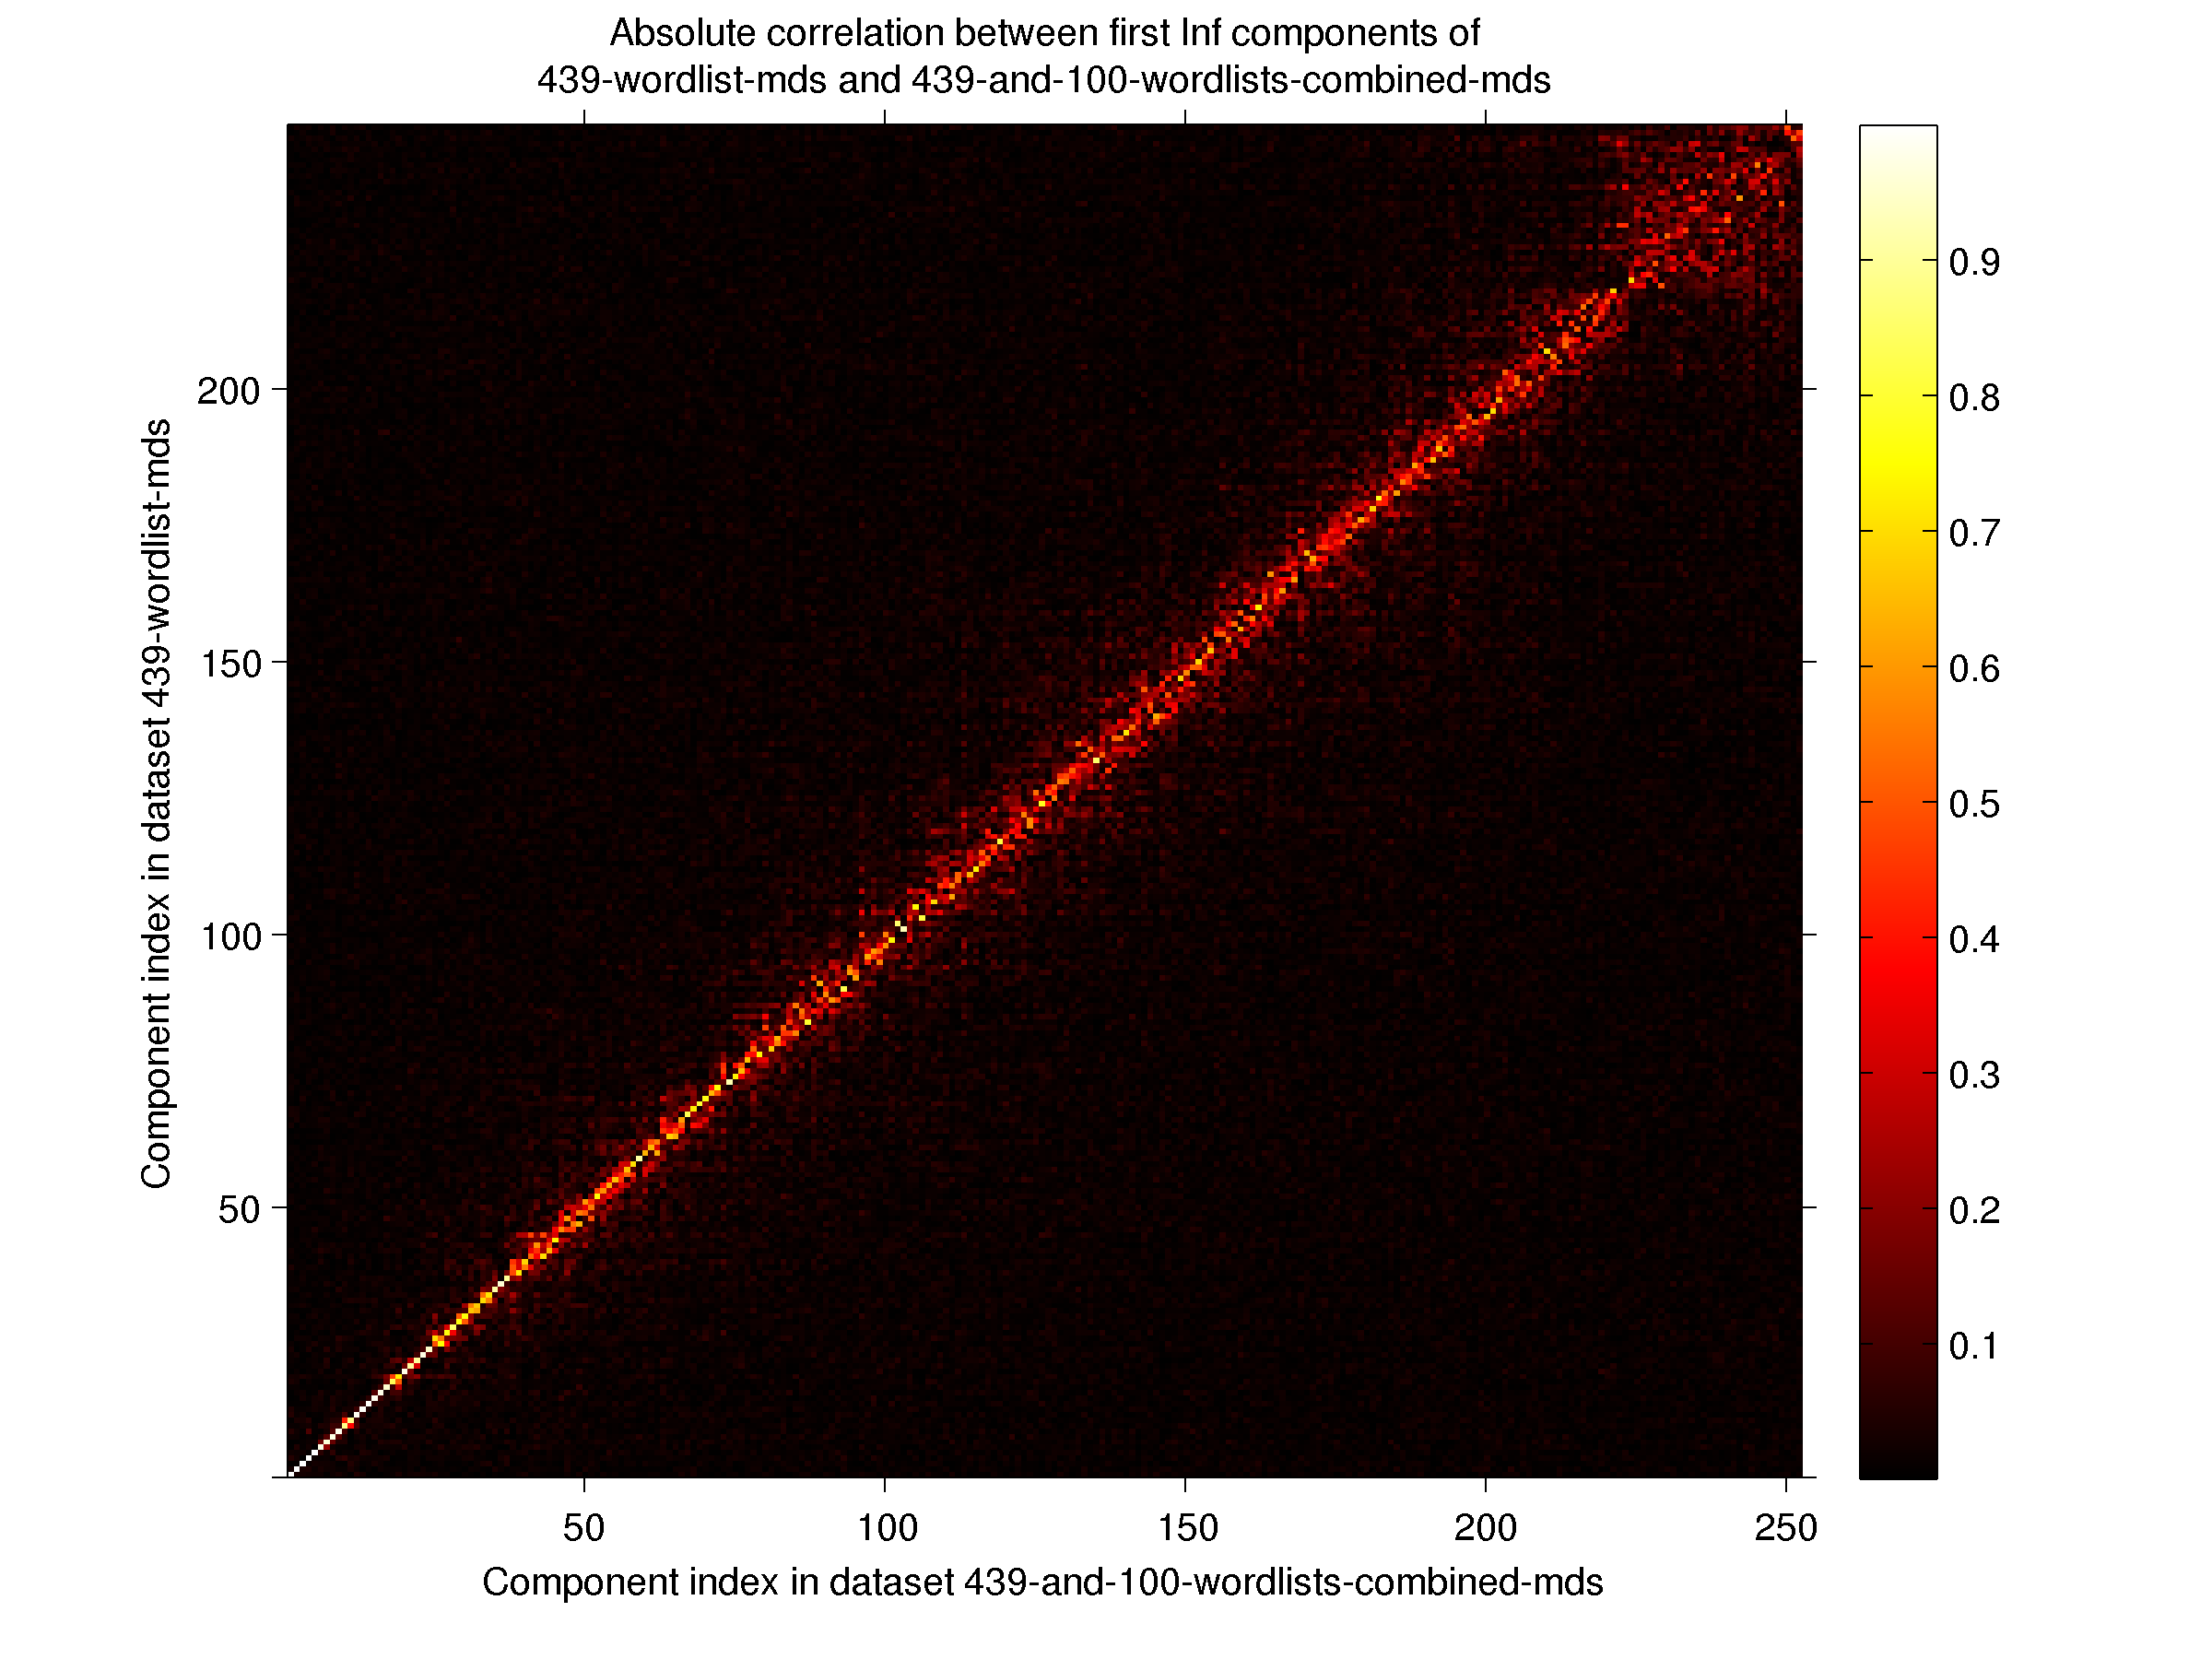
\includegraphics[width=0.9\linewidth]{439-vs-439and100-from-800dim-lowercase-wmt-model-correlations}
    \caption{Correlations between the first 52 MDS vectors generated from the 
    439 word list alone and first 52 the vectors generated from the combined
    439 word and 101 word lists.}
    \label{fig:439vs439and100}
\end{figure}

\section{2797 word set}

The 2797 word list contained adjectives and nouns. The nouns were not merely
qualities but also categories of people. With the spelling corrections and 
variants, there were 2810 words before tagging. After tagging, there were
1860 vectors generated from this list.

\subsection{Unnormalized PCA}

\begin{longtable}[!htbp]{| rllll |}
    \hline
      & \multicolumn{4}{c|}{\textbf{Component}} \\
    \textbf{Rank} & \textbf{1} & \textbf{2} & \textbf{3} & \textbf{4} \\
    \endhead
    \hline
    1 & stringent\_jj  & warm\_jj  & considerate\_jj  & loyal\_jj \\
    2 & beneficial\_jj  & elegant\_jj  & sociable\_jj  & objector \\
    3 & indirect\_jj  & vibrant\_jj  & courteous\_jj  & staunch\_jj \\
    4 & contentious\_jj  & savant  & trustworthy\_jj  & devout\_jj \\
    5 & prudent\_jj  & sparkling\_jj  & articulate\_jj  & sociable\_jj \\
    6 & dependent\_jj  & luxurious\_jj  & open-minded\_jj  & alcoholic \\
    7 & lax\_jj  & graceful\_jj  & approachable\_jj  & avid\_jj \\
    \hline
    1854 & sardonic\_jj  & slanderous\_jj  & broiler  & contrived\_jj \\
    1855 & guileless\_jj  & selfish\_jj  & soft-shelled\_jj  & didactic\_jj \\
    1856 & go-getter  & cowardly\_jj  & bendable\_jj  & defamatory\_jj \\
    1857 & self-possessed\_jj  & deceitful\_jj  & pixy  & imprecise\_jj \\
    1858 & girlish\_jj  & untruthful\_jj  & butterfly  & dissonant\_jj \\
    1859 & vivacious\_jj  & bigoted\_jj  & gingery\_jj  & limpid\_jj \\
    1860 & mousy\_jj  & defamatory\_jj  & comforter  & unvarying\_jj \\
    \hline
    \caption{The highest and lowest ranking words on the first 4 components 
    derived from unnormalized PCA of the 1860 word vectors 
    derived from the 2797 word list.} 
    \label{tab:2797wordsRankingsUnnormalizedPCA}
\end{longtable}


\begin{figure}[tbp]
    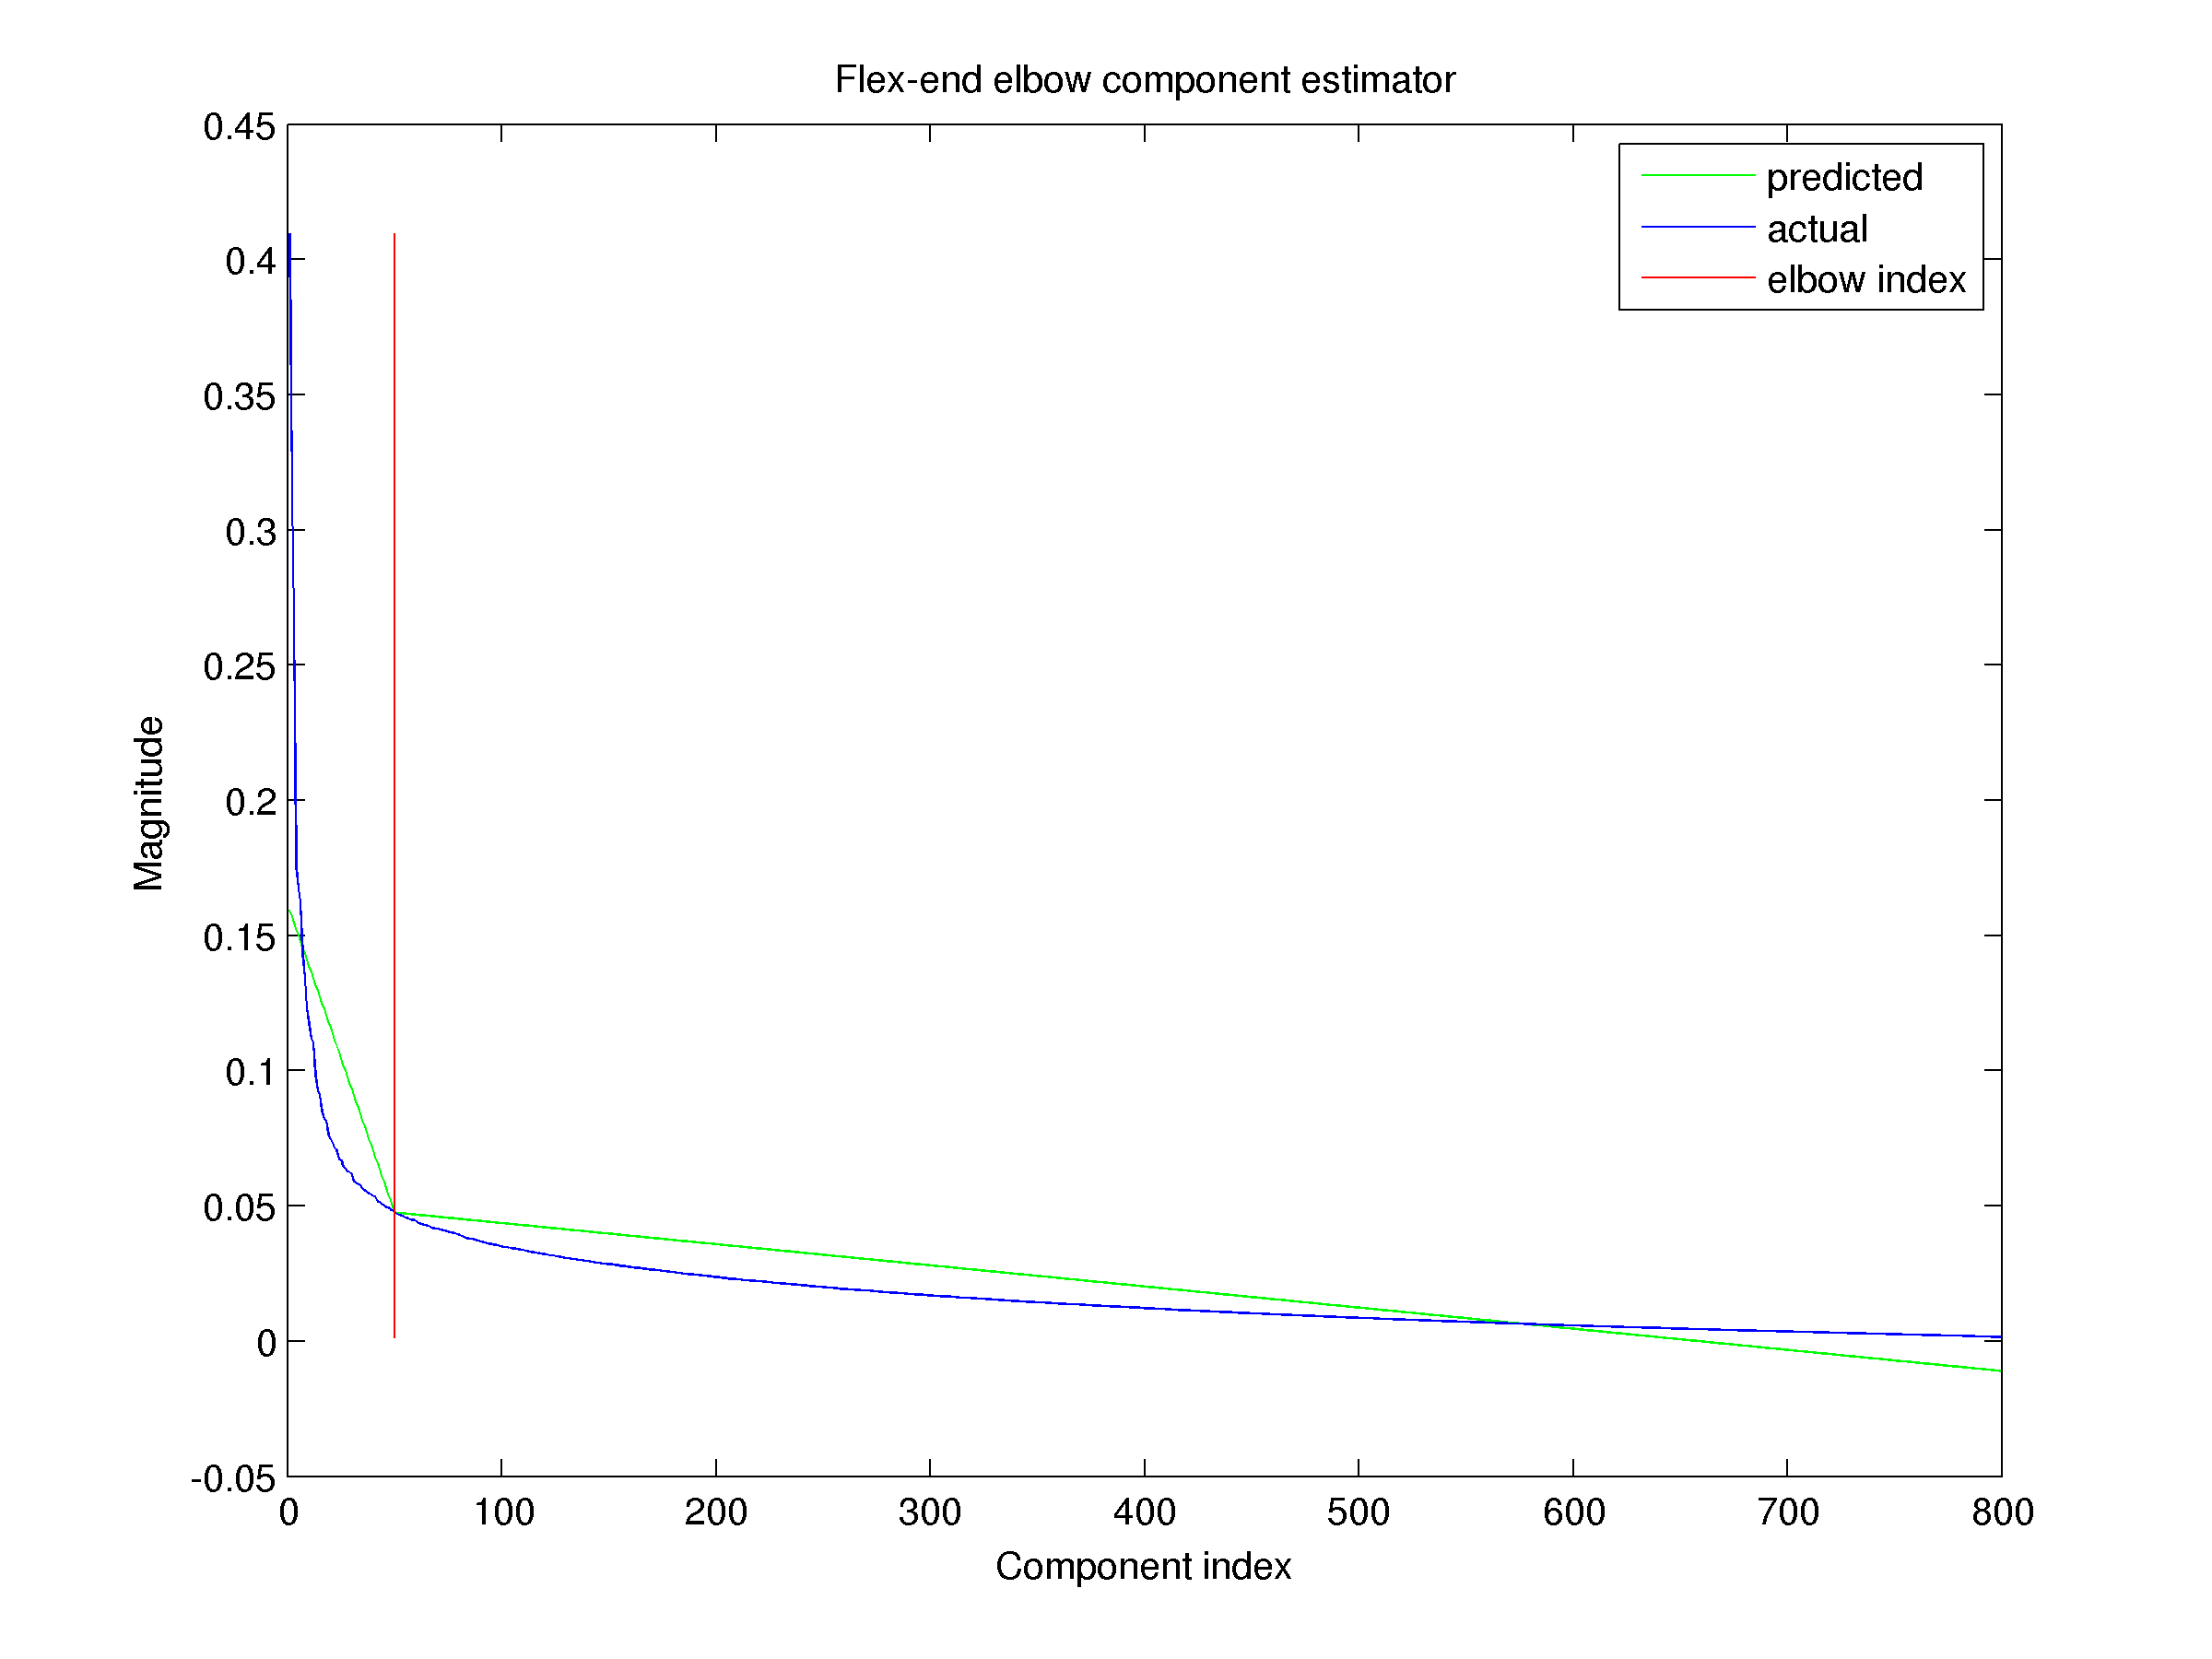
\includegraphics[width=0.9\linewidth]{2797words-adj-800dim-lowercase-wmt-model-original-flex_end_elbow}
    \caption{Eigenvalues for each principal component of the 1860 word vectors
    produced from the 2797 word list.}
    \label{fig:2797wordsunnormalizedpcaeigenvalues}
\end{figure}

Table \ref{tab:2797wordsRankingsUnnormalizedPCA} gives the highest and lowest
ranking words on the first 4 principal components of the unnormalized 1860 word 
vectors. A more complete list can be found in Appendix 
\ref{app:rankedwordlists:2797words:unnormalized}.


\subsection{Normalized PCA}

\begin{longtable}[tbp]{| rllll |}
    \hline
      & \multicolumn{4}{c|}{\textbf{Component}} \\
    \textbf{Rank} & \textbf{1} & \textbf{2} & \textbf{3} & \textbf{4} \\
    \endhead
    \hline
    1 & stringent\_jj  & warm\_jj  & considerate\_jj  & objector \\
    2 & beneficial\_jj  & elegant\_jj  & sociable\_jj  & loyal\_jj \\
    3 & indirect\_jj  & savant  & courteous\_jj  & staunch\_jj \\
    4 & contentious\_jj  & vibrant\_jj  & trustworthy\_jj  & devout\_jj \\
    5 & dependent\_jj  & luxurious\_jj  & articulate\_jj  & avid\_jj \\
    6 & prudent\_jj  & sparkling\_jj  & open-minded\_jj  & sociable\_jj \\
    7 & lax\_jj  & graceful\_jj  & approachable\_jj  & alcoholic \\
    \hline
    1854 & guileless\_jj  & inhuman\_jj  & bendable\_jj  & oblique\_jj \\
    1855 & sardonic\_jj  & slanderous\_jj  & soft-shelled\_jj  & contrived\_jj \\
    1856 & self-possessed\_jj  & deceitful\_jj  & broiler  & imprecise\_jj \\
    1857 & go-getter  & untruthful\_jj  & butterfly  & dissonant\_jj \\
    1858 & girlish\_jj  & cowardly\_jj  & pixy  & defamatory\_jj \\
    1859 & vivacious\_jj  & bigoted\_jj  & comforter  & limpid\_jj \\
    1860 & mousy\_jj  & defamatory\_jj  & gingery\_jj  & unvarying\_jj \\
    \hline
    \caption{The highest and lowest ranking words on the first 4 components 
    derived from normalized PCA of the 1860 word vectors 
    derived from the 2797 word list.} 
    \label{tab:2797wordsRankingsNormalizedPCA}
\end{longtable}


\begin{figure}[tbp]
    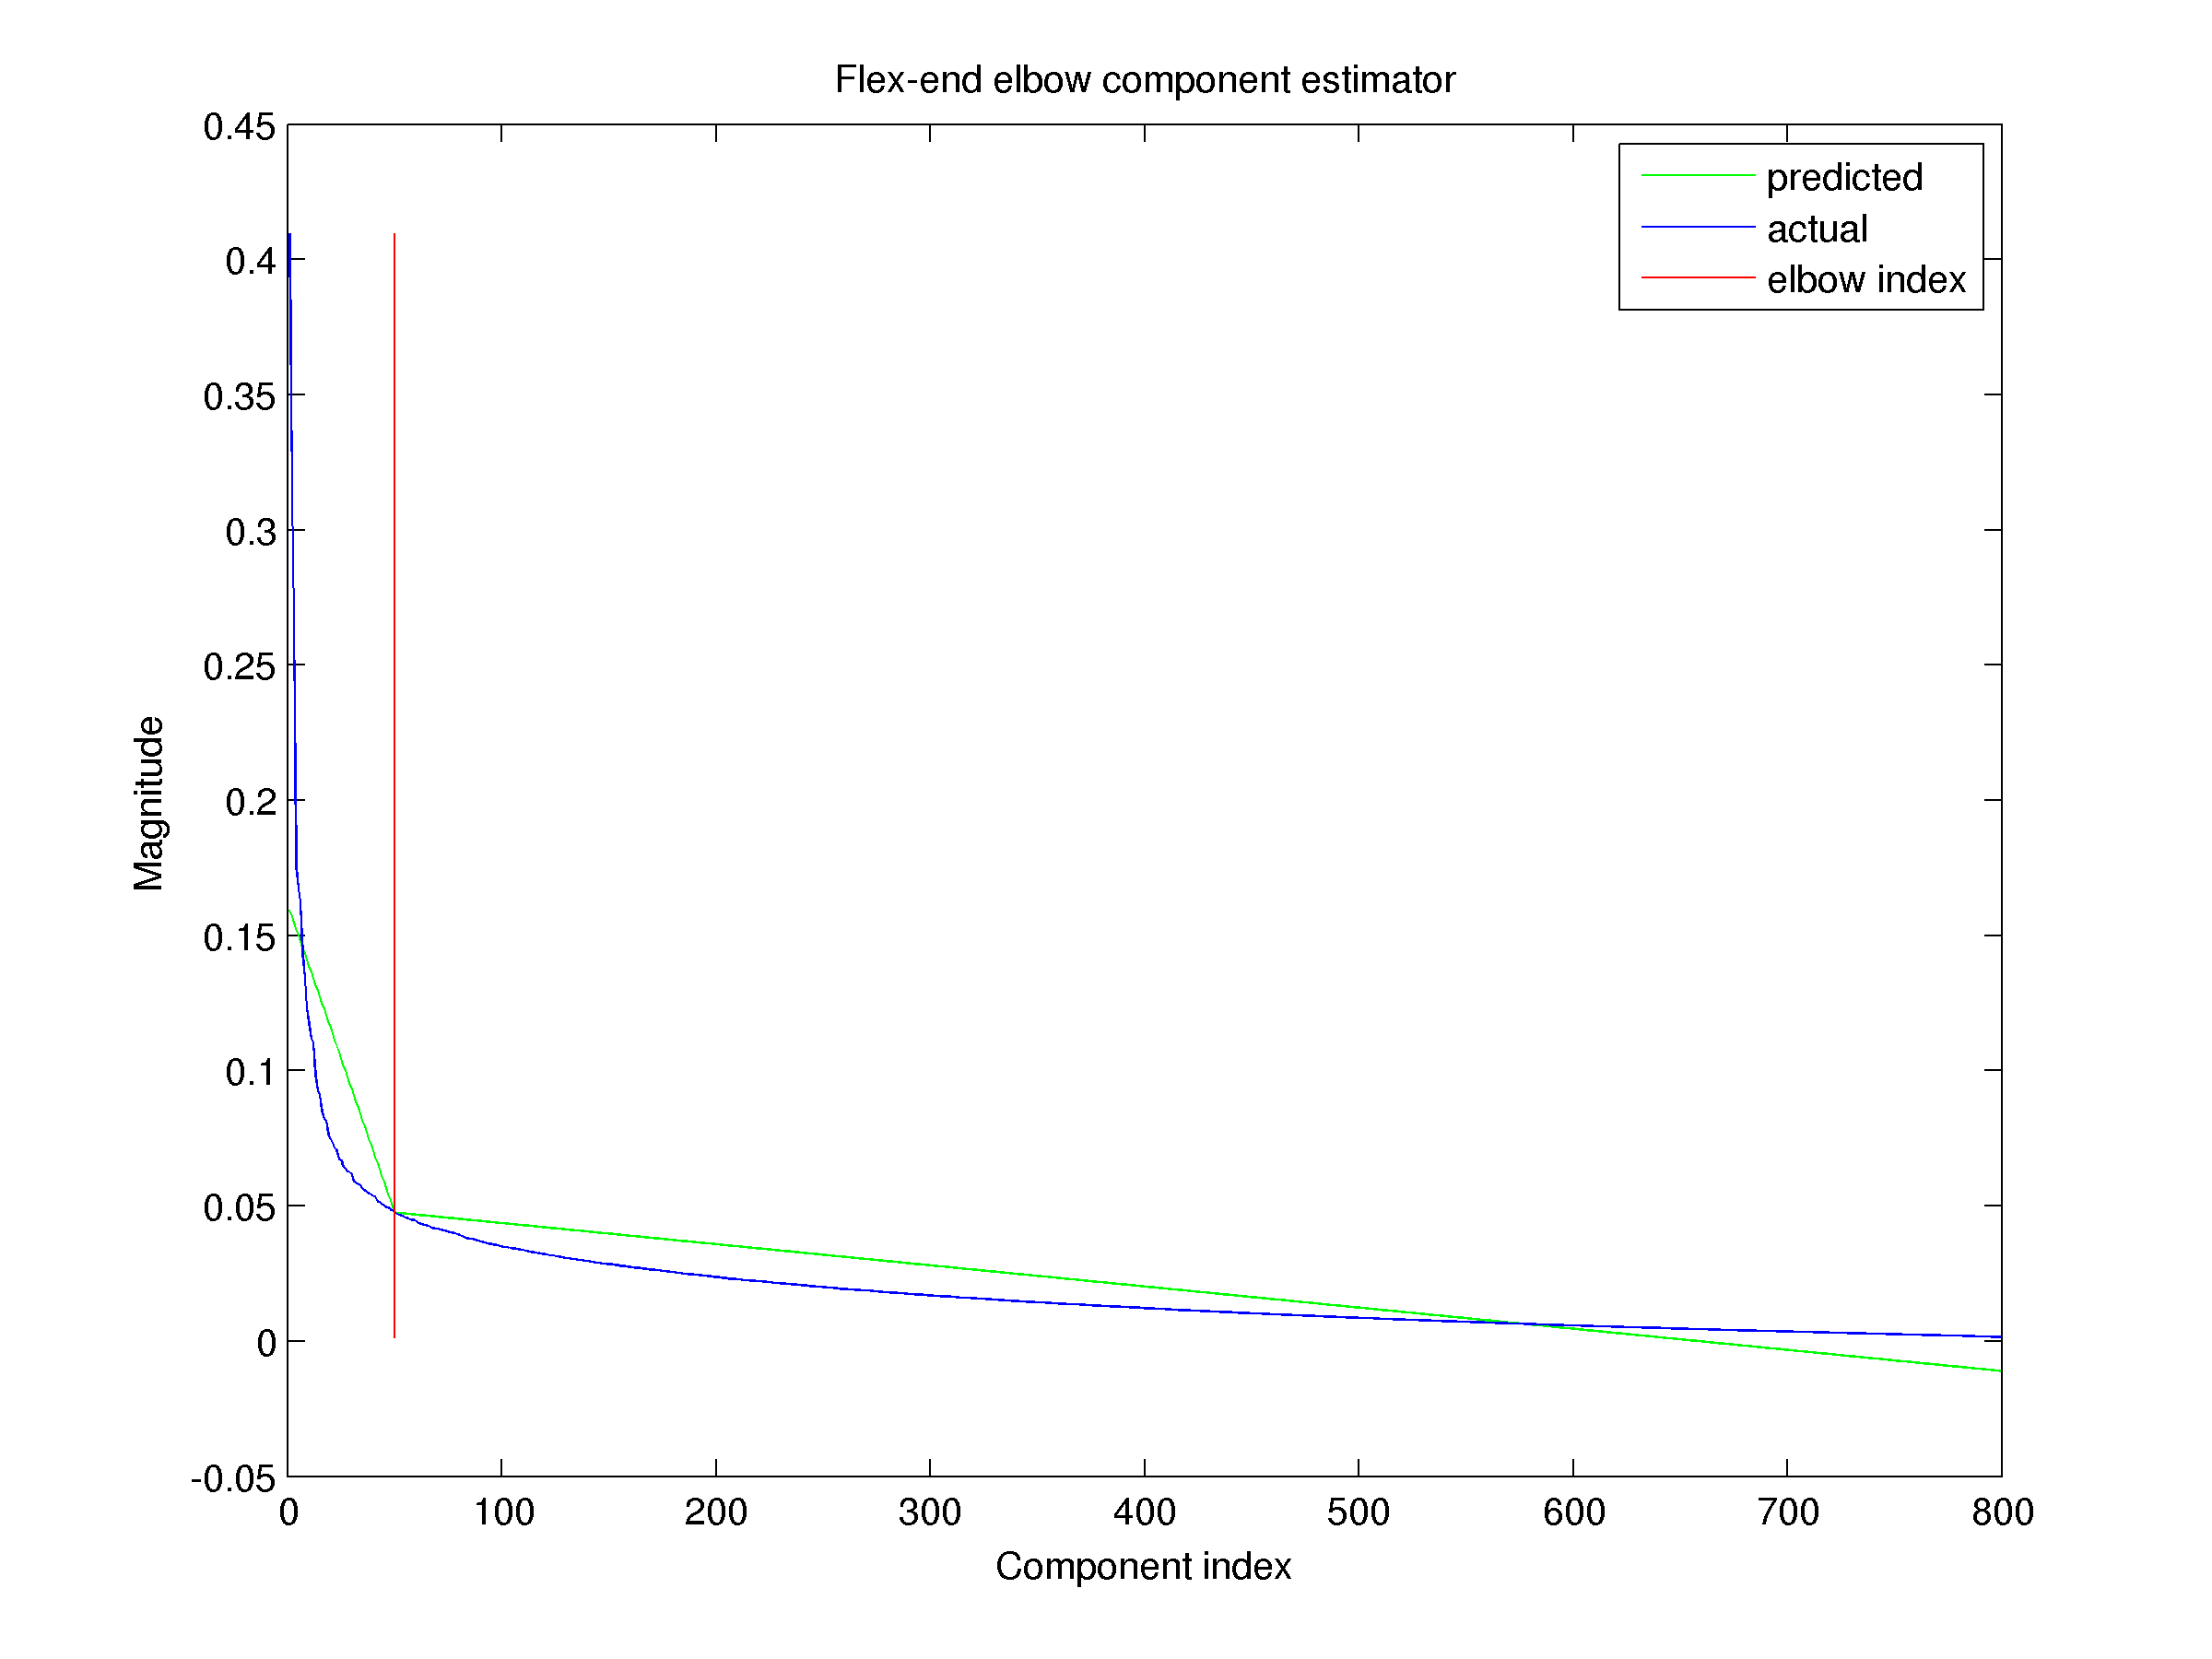
\includegraphics[width=0.9\linewidth]{2797words-adj-800dim-lowercase-wmt-model-original-flex_end_elbow}
    \caption{Eigenvalues for each principal component of the 1860 z-score 
    normalized word vectors produced from the 2797 word list.}
    \label{fig:2797wordsnormalizedpcaeigenvalues}
\end{figure}

Table \ref{tab:2797wordsRankingsNormalizedPCA} gives the highest and lowest
ranking words on the first 4 principal components of the z-score normalized 1860
word vectors. A more complete list can be found in Appendix 
\ref{app:rankedwordlists:2797words:normalized}.

\subsection{MDS}

\begin{longtable}[!htbp]{| rllll |}
    \hline
      & \multicolumn{4}{c|}{\textbf{Component}} \\
    \textbf{Rank} & \textbf{1} & \textbf{2} & \textbf{3} & \textbf{4} \\
    \endhead
    \hline
    1 & gamin  & bigoted\_jj  & thoughtful\_jj  & fan \\
    2 & coquettish\_jj  & unethical\_jj  & honest\_jj  & lucky\_jj \\
    3 & kittenish\_jj  & hypocritical\_jj  & pragmatic\_jj  & staunch\_jj \\
    4 & tender-hearted\_jj  & untruthful\_jj  & trustworthy\_jj  & bulldog \\
    5 & shrewish\_jj  & godless\_jj  & open-minded\_jj  & rowdy\_jj \\
    6 & donnish\_jj  & untransparent\_jj  & forthright\_jj  & stalwart \\
    7 & slangy\_jj  & dishonest\_jj  & articulate\_jj  & jealous\_jj \\
    \hline
    1854 & direct\_jj  & sunny\_jj  & yellow\_jj  & poetic\_jj \\
    1855 & reasonable\_jj  & polished\_jj  & butterfly  & imaginative\_jj \\
    1856 & consistent\_jj  & elegant\_jj  & gingery\_jj  & recondite\_jj \\
    1857 & contentious\_jj  & vibrant\_jj  & bendable\_jj  & assimilative\_jj \\
    1858 & prudent\_jj  & calm\_jj  & broiler  & participative\_jj \\
    1859 & stringent\_jj  & graceful\_jj  & pixy  & undogmatic\_jj \\
    1860 & beneficial\_jj  & lively\_jj  & soft-shelled\_jj  & abstract\_jj \\
    \hline
    \caption{\todo{need to caption the table for 2797words-adj-800dim-lowercase-wmt-model-mds-transformed-summary-table.tex} } \\
\end{longtable}


Table \ref{tab:2797wordsRankingsMDS} gives the highest and lowest
ranking words on the first 4 principal components of the 1860 word 
vectors after MDS. A more complete list can be found in Appendix 
\ref{app:rankedwordlists:2797words:mds}.

\begin{figure}[tbp]
    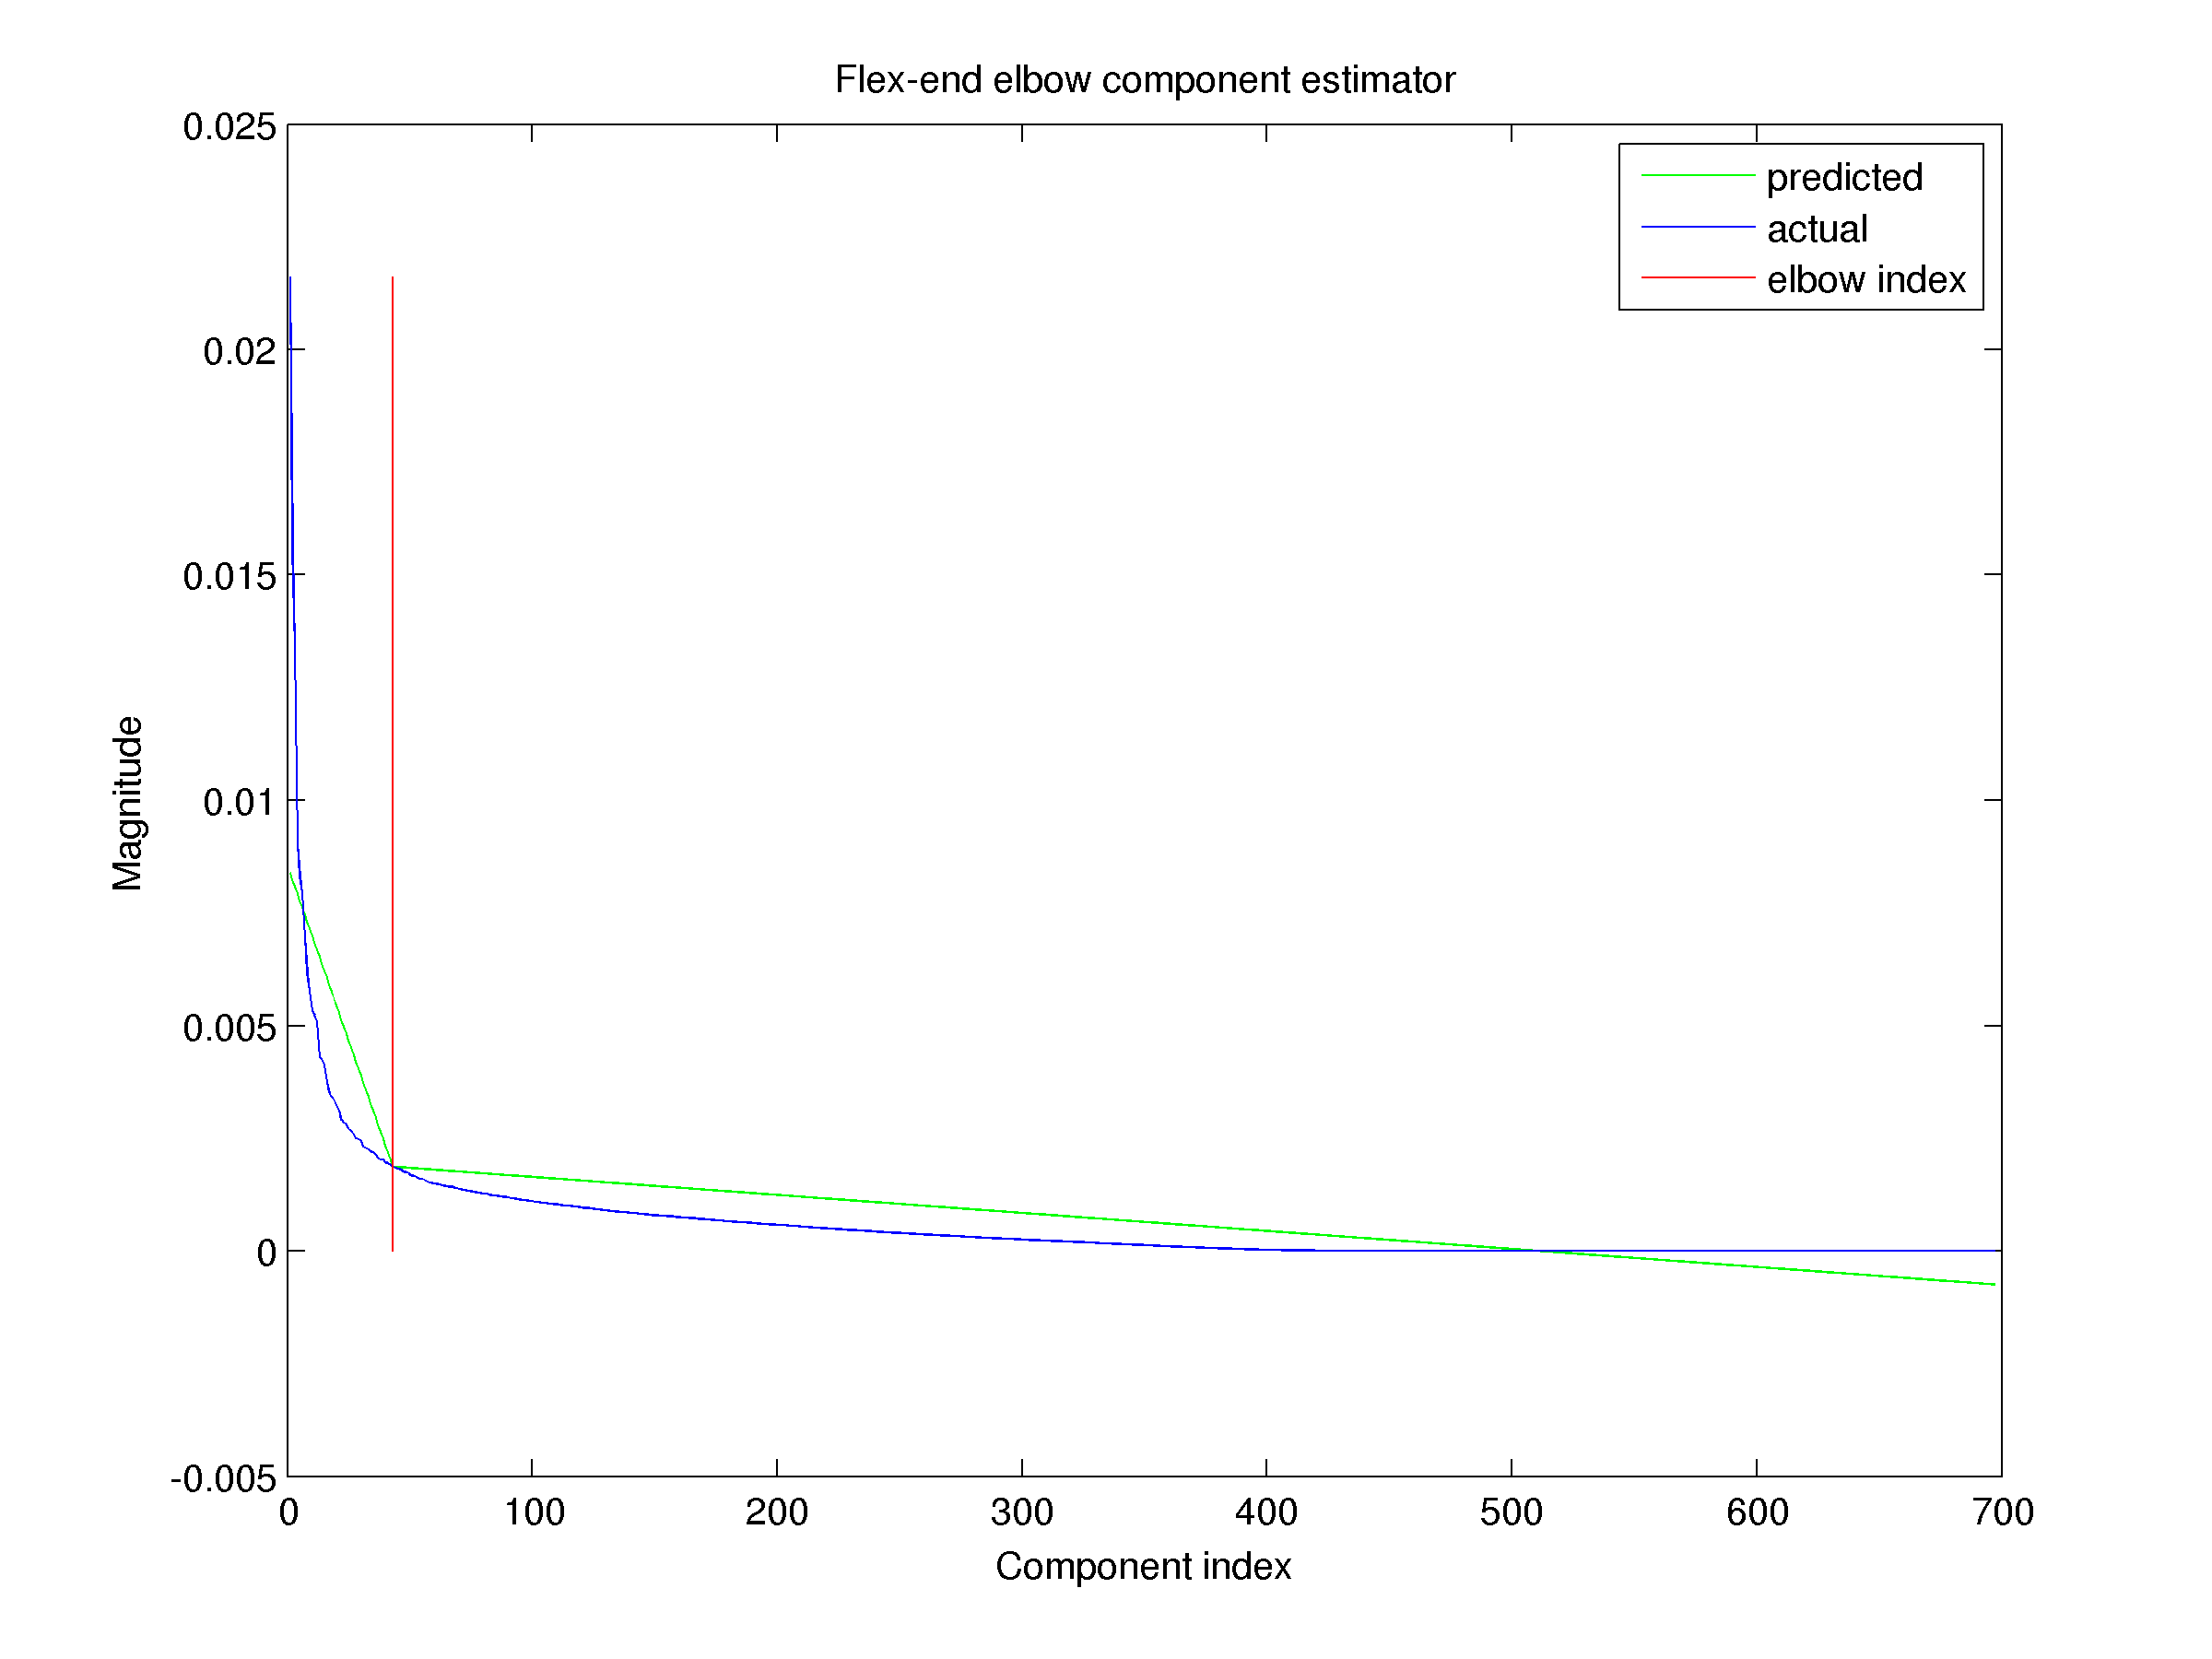
\includegraphics[width=0.9\linewidth]{2797words-adj-800dim-lowercase-wmt-model-mds-transformed-flex_end_elbow}
    \caption{Eigenvalues for each principal component of the 1860 word vectors
    produced from the 2797 word list after multidimensional scaling.}
    \label{fig:2797wordsmdseigenvalues}
\end{figure}


\section{Combined 2797, 438, and 101 word sets}

When the three word-lists are combined, it adds another 118 words, for 1978
total. The additional words are listed in Table 
\ref{tab:additionalwordsin2797combined}. Since they make up 6\% of the resulting
list, these have more effect on the resulting
components than adding 9 vectors to the 421 vectors from the 439 word list.
However, as Figure \ref{fig:2797vs2797and439and100} shows, they are still
extremely close - it is not until dimension 6 that the first noticeable
difference appears. See Appendix \ref{app:rankedwordlists:2797and438and101words}
the ranked word lists.


\begin{figure}[tbp]
    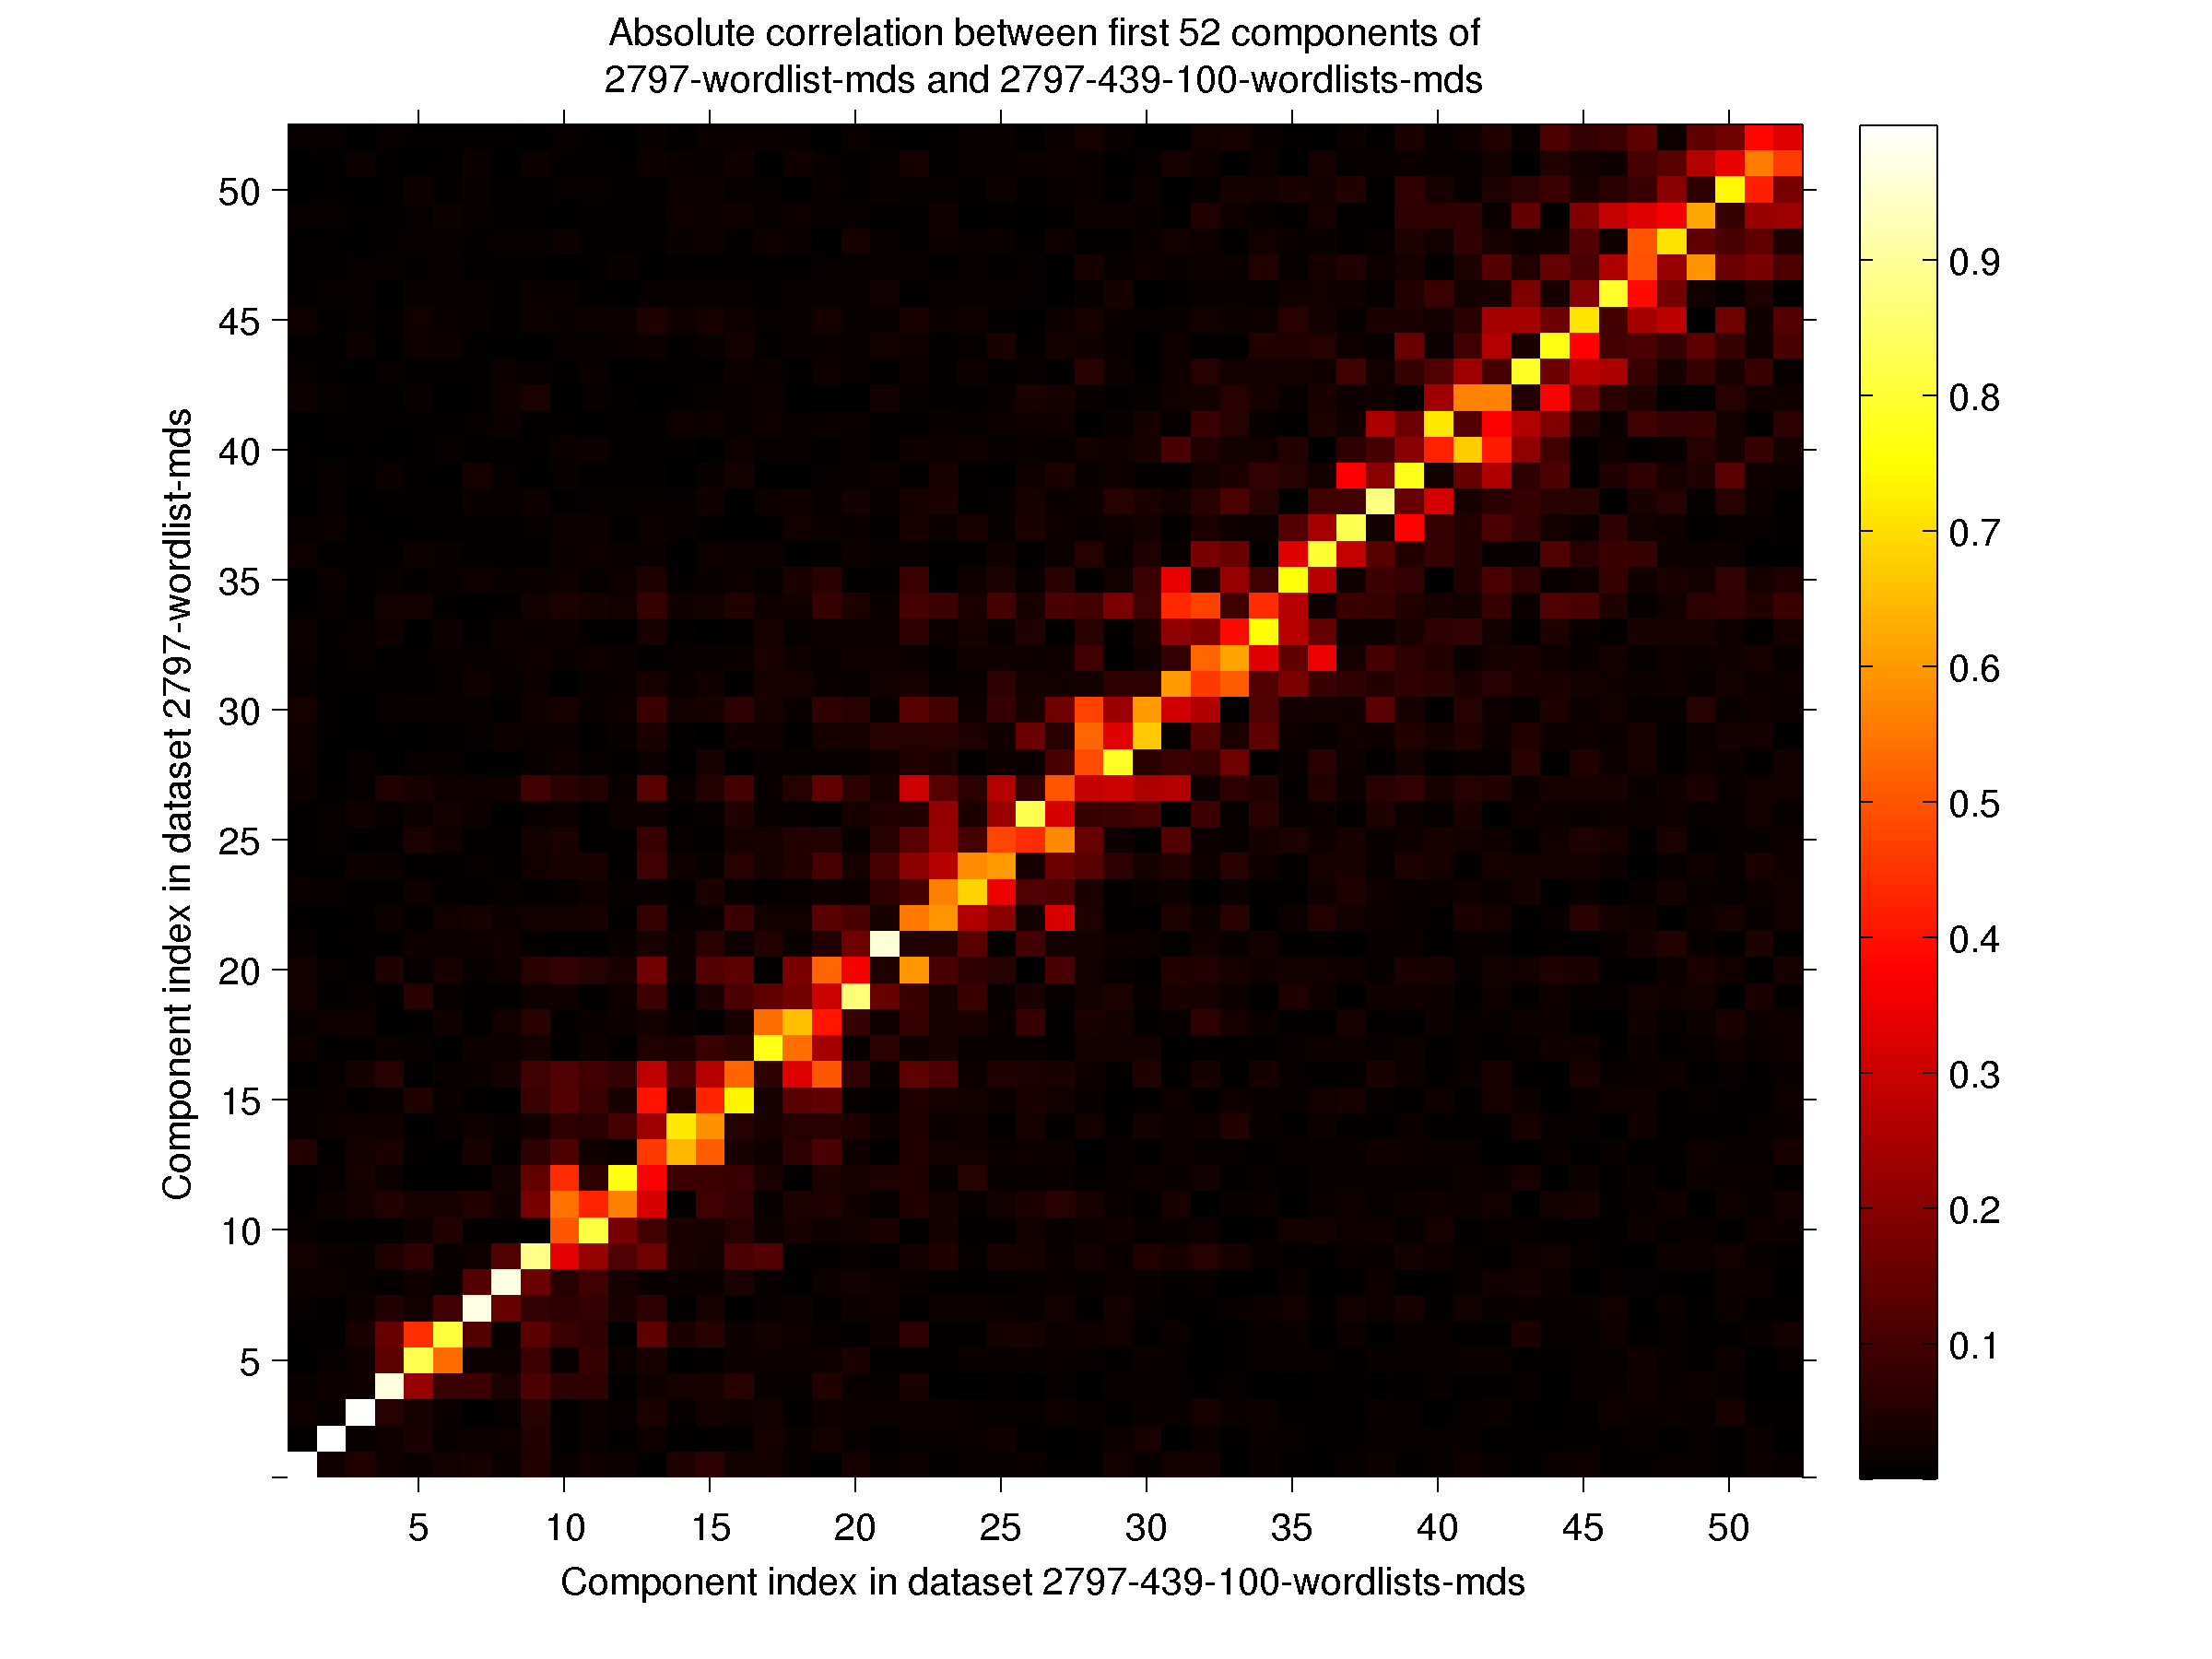
\includegraphics[width=0.9\linewidth]{2797-vs-2797and439and1100-from-800dim-lowercase-wmt-model-correlations}
    \caption{Correlations between the first 52 MDS vectors generated from the 
    2797 word list alone and the first 52 vectors generated from the combined
    2797 word, 439 word and 101 word lists.}
    \label{fig:2797vs2797and439and100}
\end{figure}


\begin{table}[tbp]
    \begin{tabular}{| llll |}
        \hline
        aimlessness & aloofness & ambition & amiability \\
        animation & anxious\_jj & assertion & belligerence \\
        bossiness & callousness & candor & caution \\
        conceit & conventionality & cooperation & courage \\
        courtesy & creativity & cruelty & curiosity \\
        deceit & decisiveness & defensive\_jj & demanding\_jj \\
        dependability & depth & dignity & disorganization \\
        distrust & dominant\_jj & dull\_jj & earthiness \\
        easygoing\_jj & efficiency & egotistical\_jj & emotionality \\
        empathy & enthusiastic\_jj & envious\_jj & envy \\
        erratic\_jj & exhibitionistic\_jj & expressiveness & fear \\
        fearful\_jj & flexibility & forgetfulness & frivolity \\
        generosity & gregariousness & gullibility & humor \\
        humorous\_jj & inconsistency & indecisiveness & independence \\
        inhibition & insecurity & insight & instability \\
        intellectuality & intelligence & intrusiveness & irritability \\
        leniency & lethargy & logic & modest\_jj \\
        modesty & morality & naïve\_jj & natural\_jj \\
        naturalness & negligence & nonconformity & opportunistic\_jj \\
        optimism & organization & organized\_jj & passivity \\
        persistence & pessimism & placidity & playfulness \\
        pomposity & precision & predictability & prejudice \\
        prejudiced\_jj & punctuality & quiet & recklessness \\
        reserve & rudeness & self-esteem & selfishness \\
        shallowness & shyness & silence & simple\_jj \\
        sloth & smart\_jj & sophistication & spirit \\
        spontaneity & stinginess & stubbornness & stupidity \\
        surliness & talkativeness & thoughtlessness & thrift \\
        underhanded\_jj & understanding & unfriendliness & volatility \\
        warmth & neat\_jj &  &  \\
        \hline
    \end{tabular}
    \caption{The 181 words not present in the 1860 word vectors derived from
    the tagged 2797 word list}
    \label{tab:additionalwordsin2797combined}

\end{table}



\section{Dimension Matching}
\subsection{Overview}

As mentioned in Section \ref{sec:matchingcomponents}, I looked at the
matches between the principal components discovered in the different
wordlists as a validation as to whether the same semantics were being
covered and as an indication of how many dimensions might be
significant.

\subsection{439 and 100 vs 2797}

I began my comparison of the various dimensions with a comparison of all 
components of the combined 439 and 100 word datasets with all of the components
of the 2797 word dataset. There is a pretty dense collection of matches at
dimension less than 52 in the 2797 word list. See Figure 
\ref{fig:439and100vs2797} and Table
\ref{439and100-vs-2797-from-800dim-lowercase-wmt-model-significant.tex}. 

\begin{table}[!tbp]
    \begin{tabular}{| p{0.75in}p{3.5in} |}
        \hline
        \textbf{439-and-100-wordlists-combined-mds dim} & \textbf{2797-wordlist-mds -- dim(correlation)}\\
        1 & 1(0.95), 3(0.33)\\
        2 & 2(-0.88), 3(0.32), 5(-0.34)\\
        3 & 2(0.65), 3(0.32), 4(0.42), 6(0.5), 16(0.29)\\
        4 & 4(-0.53), 7(0.54), 8(-0.46)\\
        5 & 3(-0.47), 4(-0.47), 7(-0.43), 8(-0.36), 10(0.37), 11(-0.35), 13(-0.3), 25(-0.31)\\
        6 & 5(-0.81), 11(-0.33), 18(0.3)\\
        7 & 4(0.32), 8(-0.47), 9(0.51), 12(0.36), 14(0.33)\\
        8 & 6(0.66), 7(0.31), 11(0.3)\\
        9 & 3(0.34), 4(-0.33), 6(0.29), 12(0.49), 14(0.4)\\
        10 & 8(0.47), 9(0.49)\\
        11 & 6(-0.31), 10(-0.59)\\
        12 & 7(0.33), 11(-0.43), 14(0.34)\\
        13 & 15(-0.4), 17(-0.43), 18(0.3), 21(0.39), 22(-0.43), 23(-0.33)\\
        14 & 11(0.4), 14(0.37)\\
        15 & 13(-0.56), 28(0.3)\\
        16 & 20(0.33), 24(0.29), 26(-0.3), 29(-0.38), 33(-0.29)\\
        18 & 15(-0.36), 19(0.36), 32(-0.3)\\
        19 & 16(-0.51), 41(0.29)\\
        20 & 26(0.3), 35(-0.37)\\
        21 & 17(-0.31), 19(0.29), 22(0.3)\\
        23 & 12(0.31), 20(0.31)\\
        24 & 23(-0.28), 40(0.34)\\
        25 & 39(0.3)\\
        26 & 35(0.29)\\
        27 & 29(-0.35)\\
        29 & 32(0.31)\\
        30 & 34(-0.4)\\
        31 & 112(-0.3)\\
        32 & 52(0.29)\\
        34 & 27(-0.3)\\
        35 & 74(0.3)\\
        37 & 37(0.3)\\
        46 & 50(0.31)\\
        62 & 83(0.29)\\
        66 & 93(0.3)\\
        77 & 177(0.3)\\
        81 & 178(-0.29)\\
        \hline
    \end{tabular}
    \caption{Dimensions from dataset 439-and-100-wordlists-combined-mds which had a significant correlation with a dimension from dataset 2797-wordlist-mds when all pairs of dimensions were considered with FDR controlled at 1\%. Each entry gives the matching dimension and the correlation between them.}
    \label{439and100-vs-2797-from-800dim-lowercase-wmt-model-significant.tex}
\end{table}


\begin{figure}[tbp]
    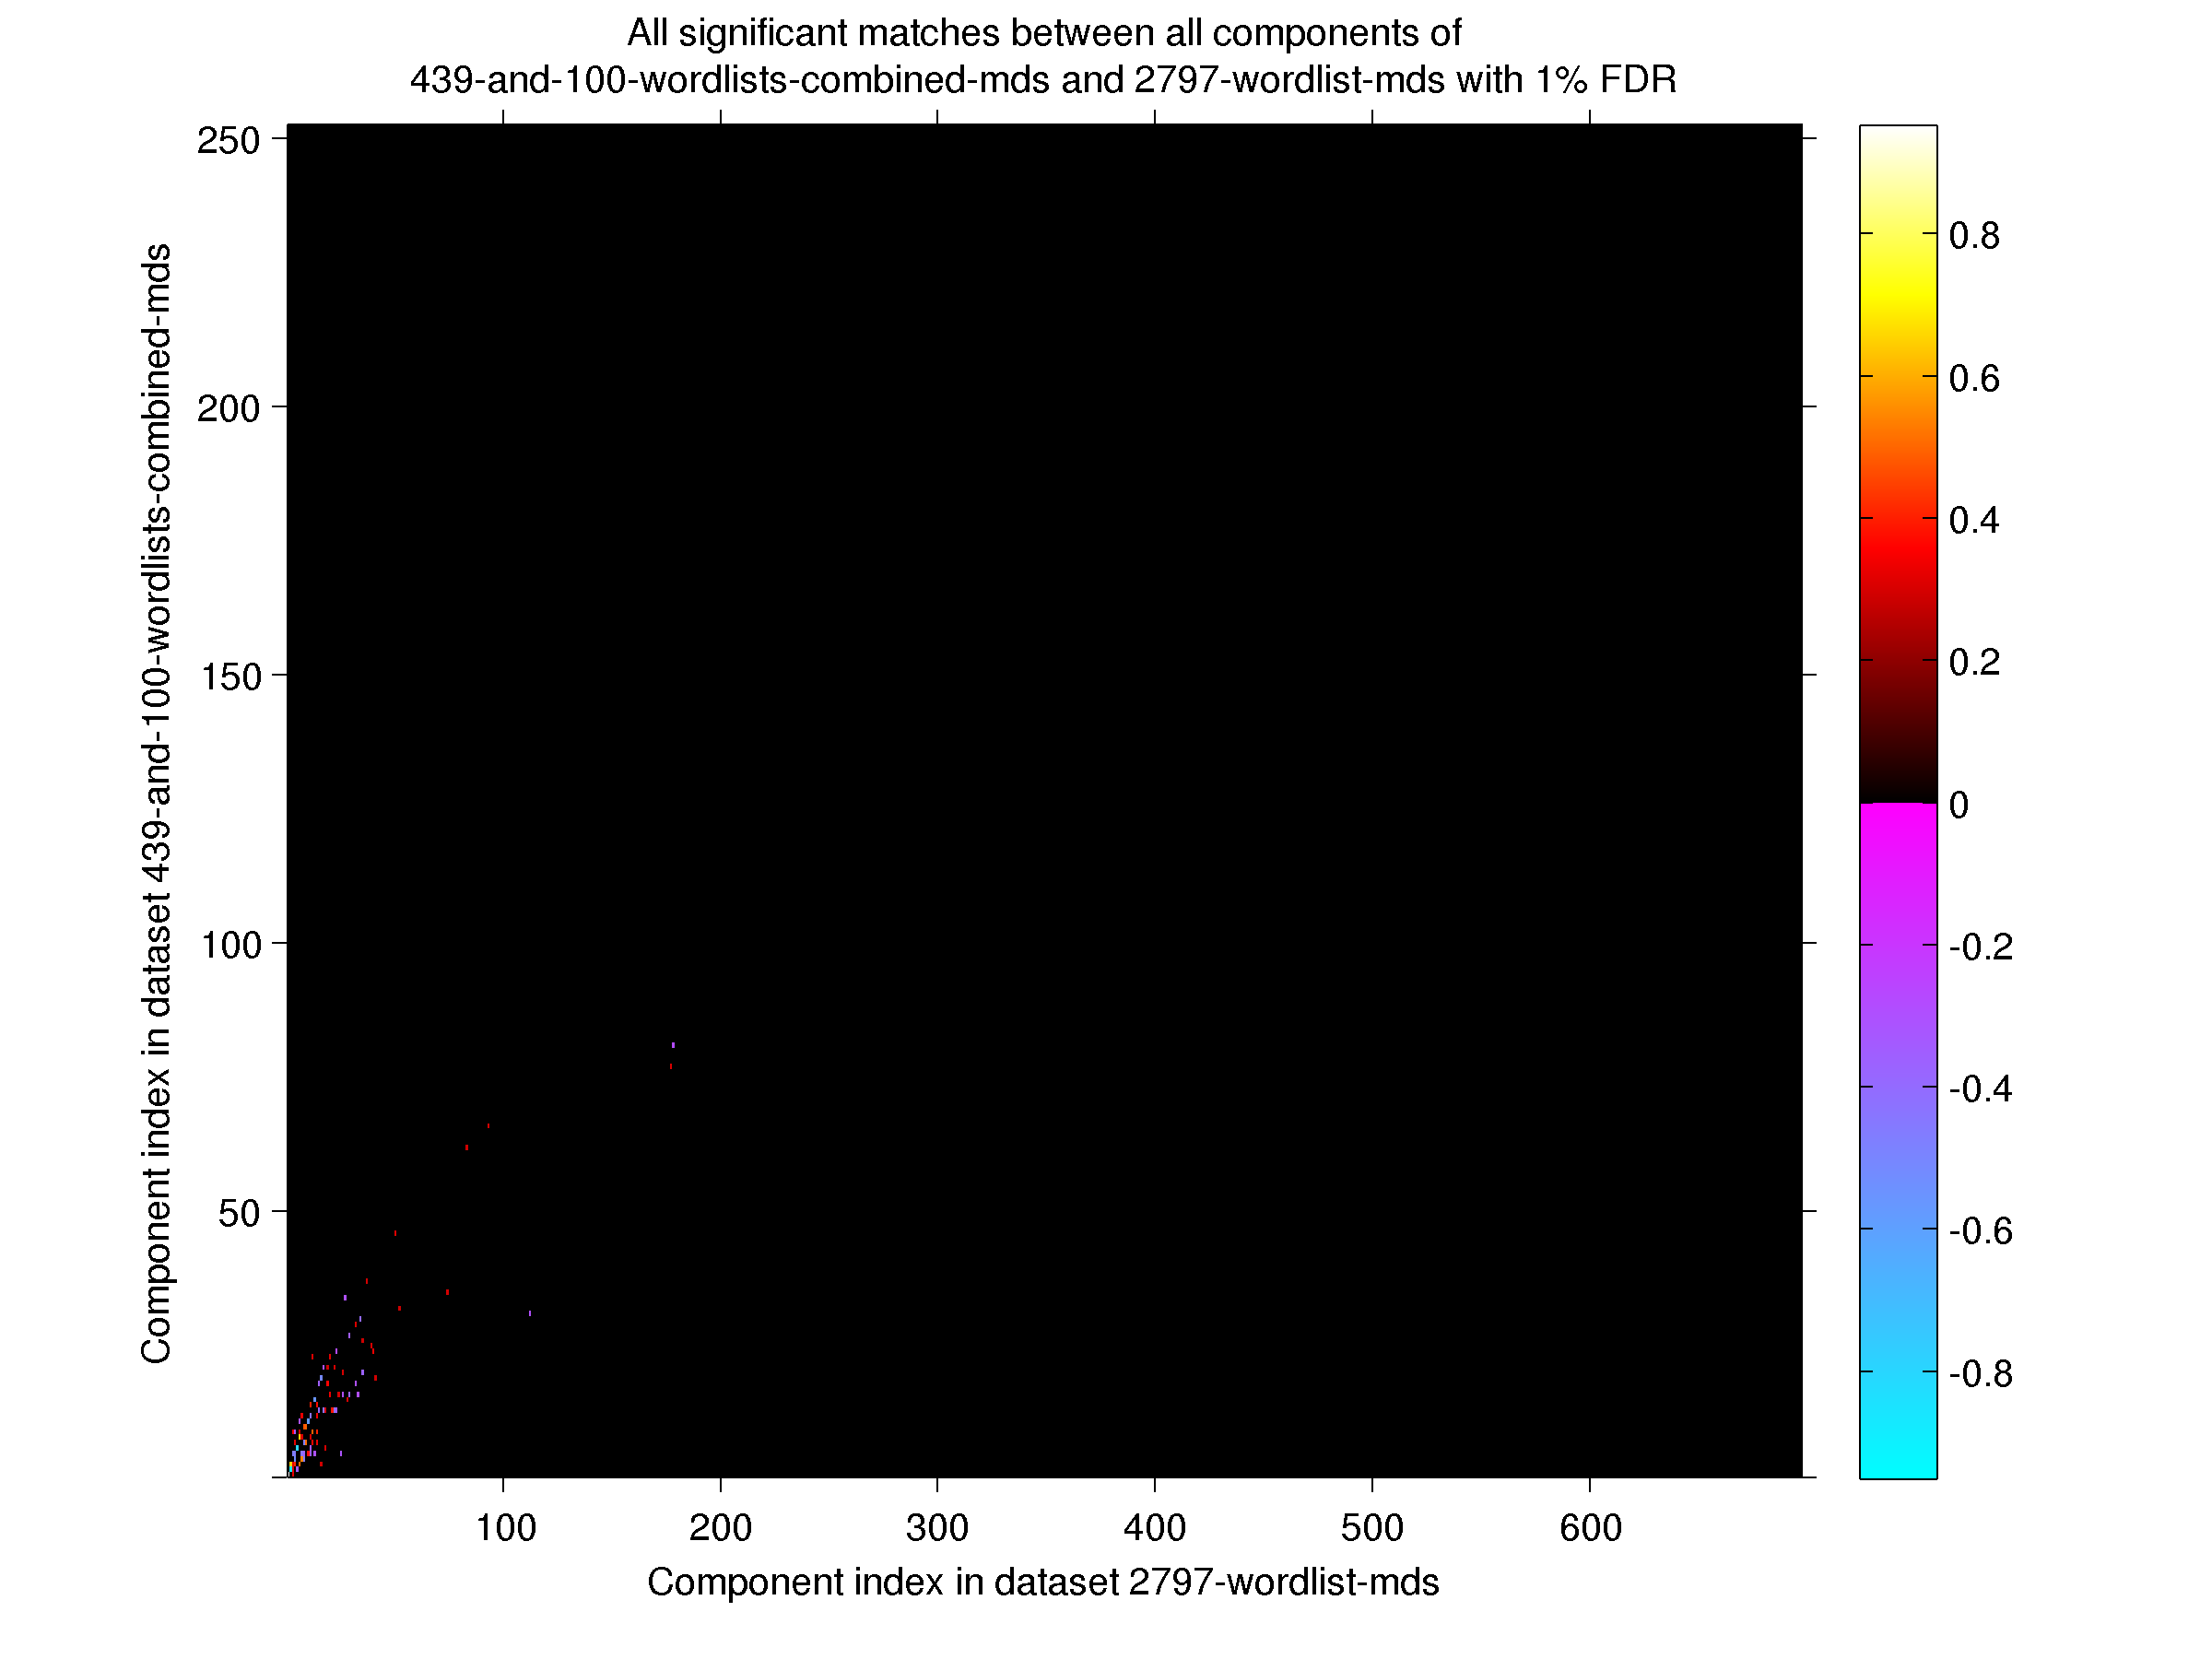
\includegraphics[width=0.9\linewidth]{439and100-vs-2797-from-800dim-lowercase-wmt-model-significant}
    \caption{Results from Table 
    \ref{439and100-vs-2797-from-800dim-lowercase-wmt-model-significant.tex} 
    displayed as an image. Colors (except black) give correlation for matching 
    dimensions.}
    \label{fig:439and100vs2797}
\end{figure}

\subsection{First 52 dimensions of 100 vs 439 and 100}

Because of the previous plot, I eliminate all but the first 52 dimensions in
looking at the components of 100 words that also appear in the combined 439
and 100 word list. This gives a relatively dense set of correspondences for the
first 22 dimensions of the combined lists (and the first 16 of the 100 word
list). See Figure \ref{fig:100vs439And100First52} and Table 
\ref{100-vs-439and100-from-800dim-lowercase-wmt-model-significant-first-52.tex}.

\begin{table}[!tbp]
    \begin{tabular}{| p{0.75in}p{3.5in} |}
        \hline
        \textbf{100-wordlist-mds dim} & \textbf{439-and-100-wordlists-combined-mds -- dim(correlation)}\\
        1 & 1(0.87), 3(0.46), 4(-0.47)\\
        2 & 2(0.87), 3(-0.56)\\
        3 & 4(0.62), 5(0.6)\\
        4 & 6(0.46), 7(-0.5), 8(-0.48)\\
        5 & 8(0.45), 11(-0.52), 13(-0.56)\\
        7 & 10(0.51)\\
        8 & 7(0.54)\\
        9 & 6(0.64)\\
        11 & 36(-0.46)\\
        12 & 10(-0.46)\\
        14 & 21(0.48), 39(-0.52)\\
        16 & 22(0.49)\\
        29 & 42(-0.47)\\
        30 & 52(0.47)\\
        \hline
    \end{tabular}
    \caption{Dimensions from dataset 100-wordlist-mds which had a significant correlation with a dimension from dataset 439-and-100-wordlists-combined-mds when only the first 52 dimensions were considered as potential matches for one another with FDR controlled at 1\%. Each entry gives the matching dimension and the correlation between them.}
    \label{100-vs-439and100-from-800dim-lowercase-wmt-model-significant-first-52.tex}
\end{table}


\begin{figure}[tbp]
    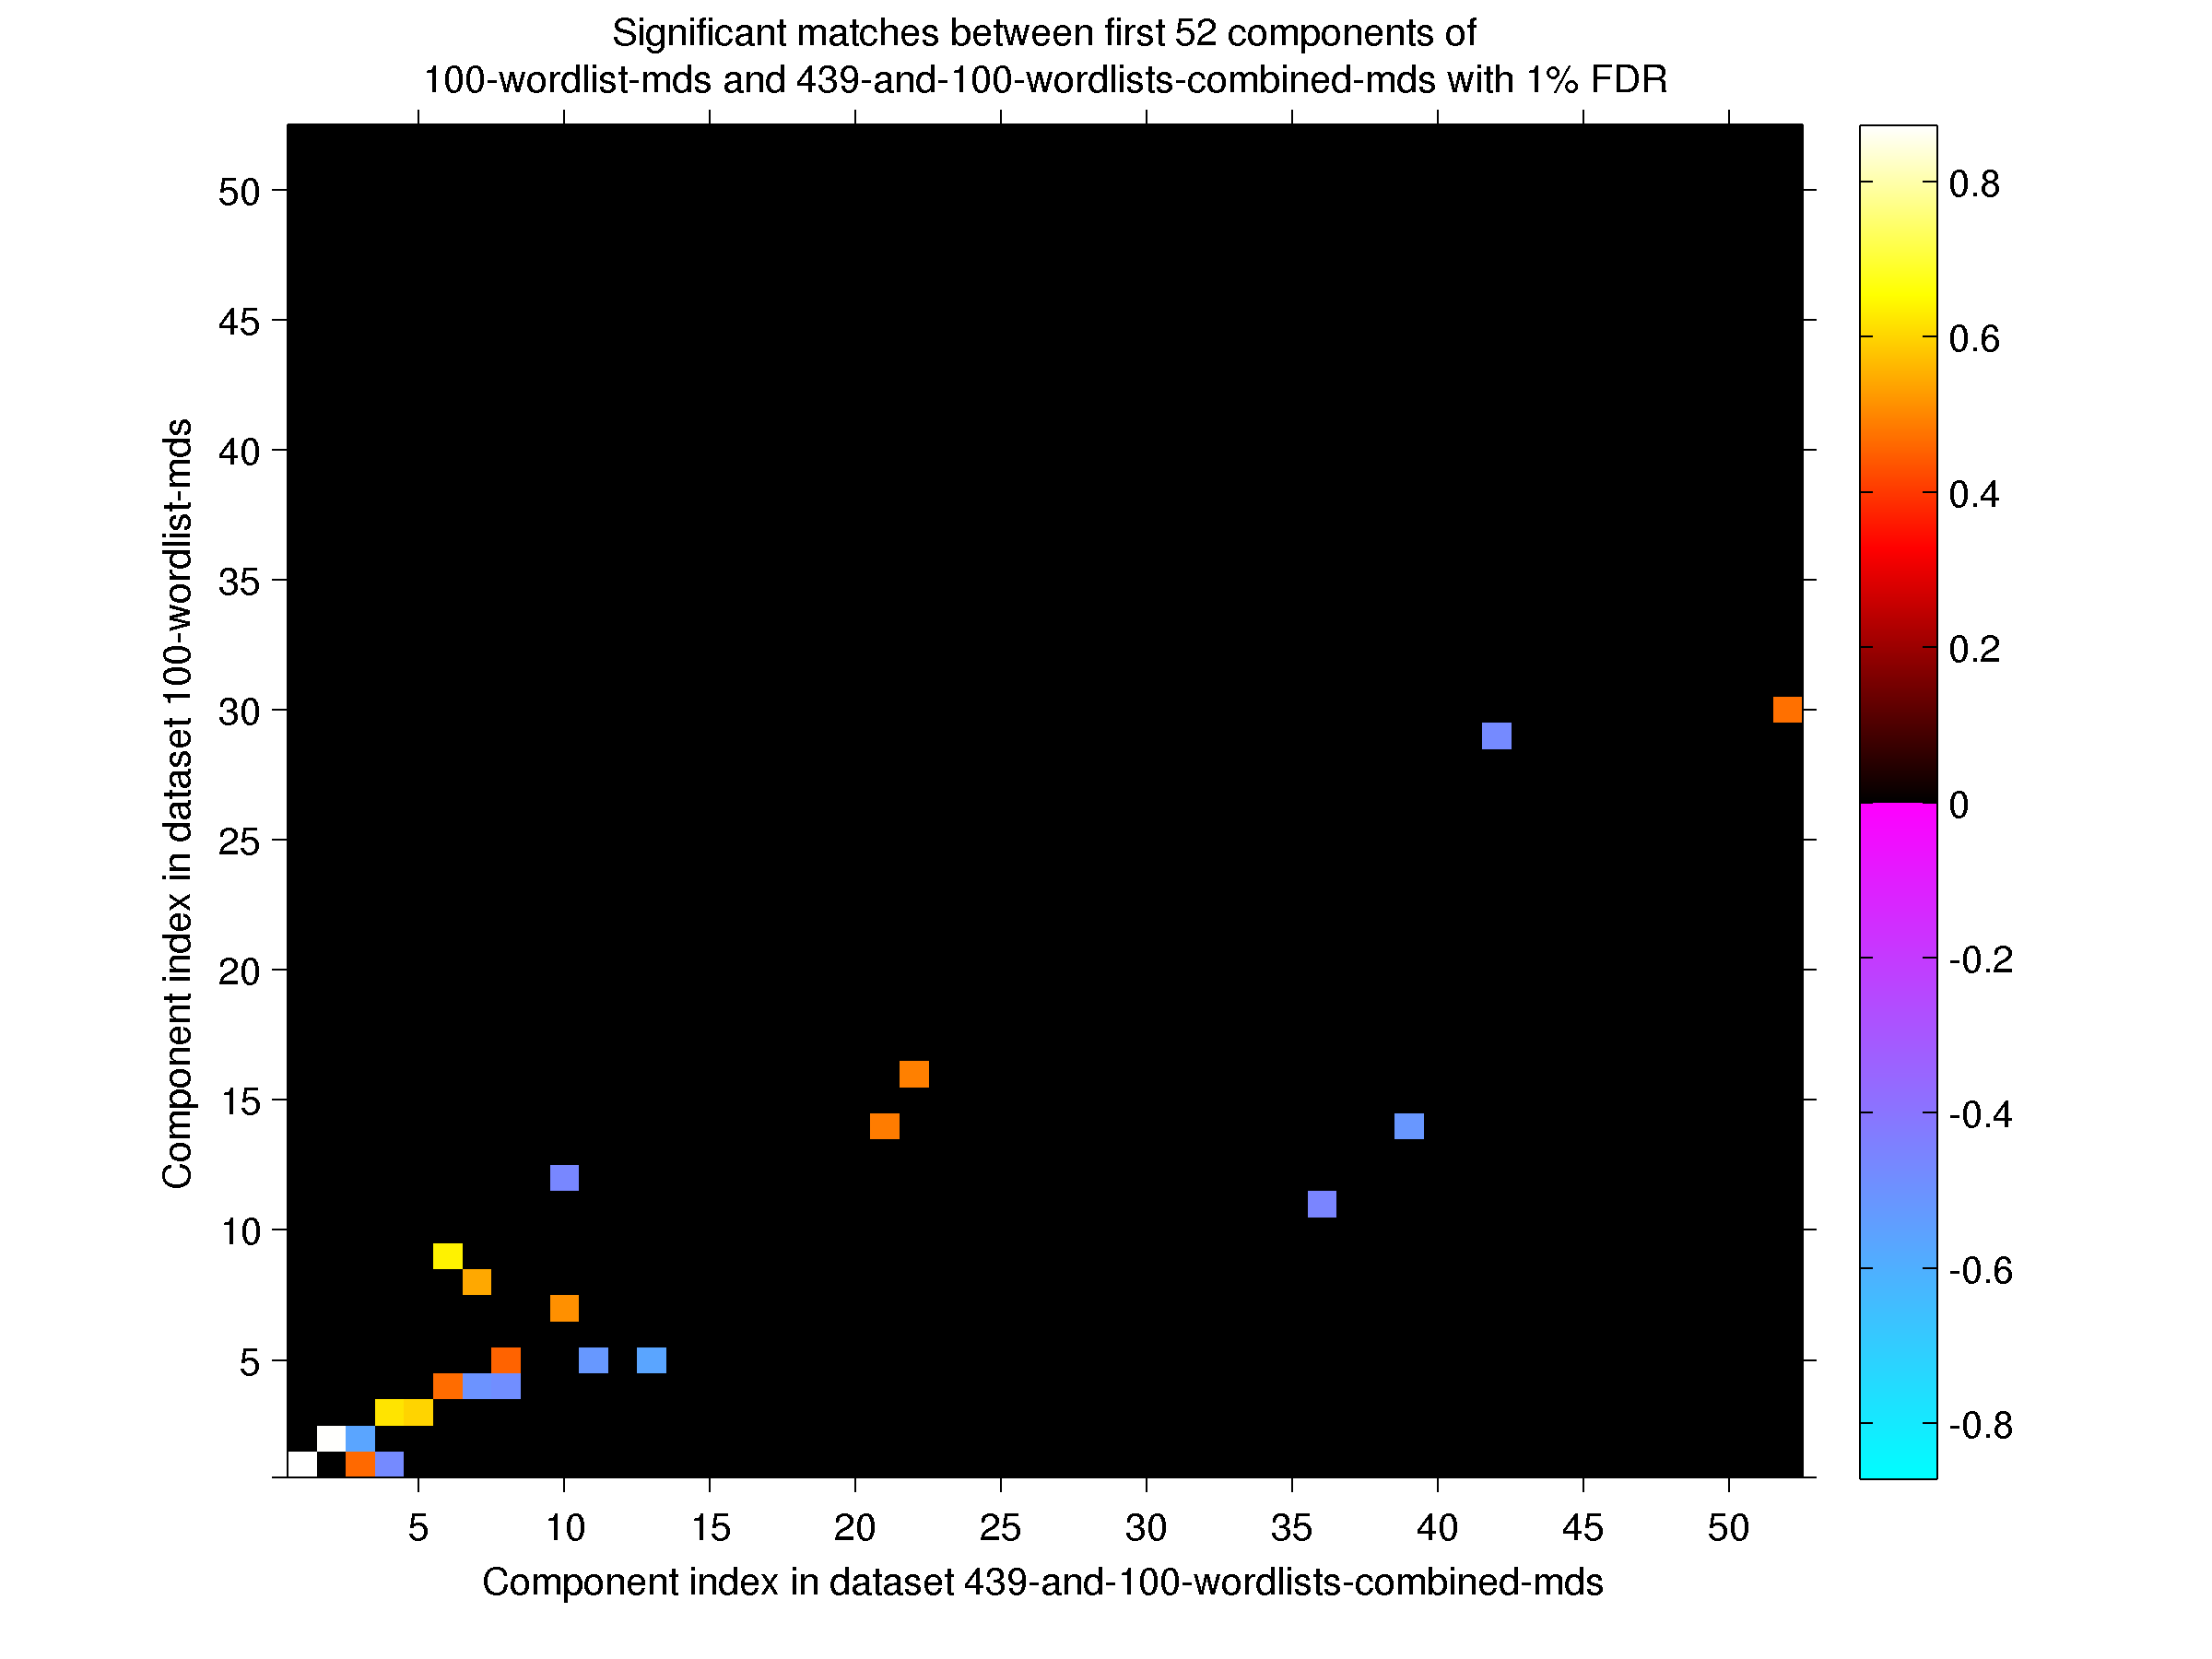
\includegraphics[width=0.9\linewidth]{100-vs-439and100-from-800dim-lowercase-wmt-model-significant-first-52}
    \caption{Results from Table 
    \ref{100-vs-439and100-from-800dim-lowercase-wmt-model-significant-first-52.tex} 
    displayed as an image. Colors (except black) give correlation for matching 
    dimensions.}
    \label{fig:100vs439And100First52}
\end{figure}

\subsection{First 22 dimensions of 100 vs 2797}

Finally, I look at only the matches between the first 22 dimensions of the
100 words and 2797 word datasets. Most of the components of the 2797 word list 
(with the exceptions of 2, 5, and 8 which have 2) have one match from the 100 
word list. This gives the 2797 word list 1.2 matches per component on average
vs. 1.7 for the 100 word list.
See Figure \ref{fig:100vs2797First22} and
Table 
\ref{100-vs-2797-from-800dim-lowercase-wmt-model-significant-first-22.tex}.


\begin{table}[!tbp]
    \begin{tabular}{| ll |}
        \hline
        \textbf{100-wordlist-mds dim} & \textbf{2797-wordlist-mds -- dim(correlation)}\\
        1 & 1(0.78), 2(0.48)\\
        2 & 2(-0.81)\\
        3 & 4(-0.69), 8(-0.55)\\
        4 & 3(0.47), 5(-0.52), 18(0.46), 21(-0.44)\\
        5 & 6(0.71), 12(-0.47), 17(0.49)\\
        6 & 7(-0.52)\\
        7 & 14(0.49)\\
        8 & 8(-0.48)\\
        9 & 5(-0.5)\\
        11 & 13(-0.6)\\
        \hline
    \end{tabular}
    \caption{Dimensions from dataset 100-wordlist-mds which had a significant correlation with a dimension from dataset 2797-wordlist-mds when only the first 22 dimensions were considered as potential matches for one another with FDR controlled at 1\%. Each entry gives the matching dimension and the correlation between them.}
    \label{100-vs-2797-from-800dim-lowercase-wmt-model-significant-first-22.tex}
\end{table}


\begin{figure}[tbp]
    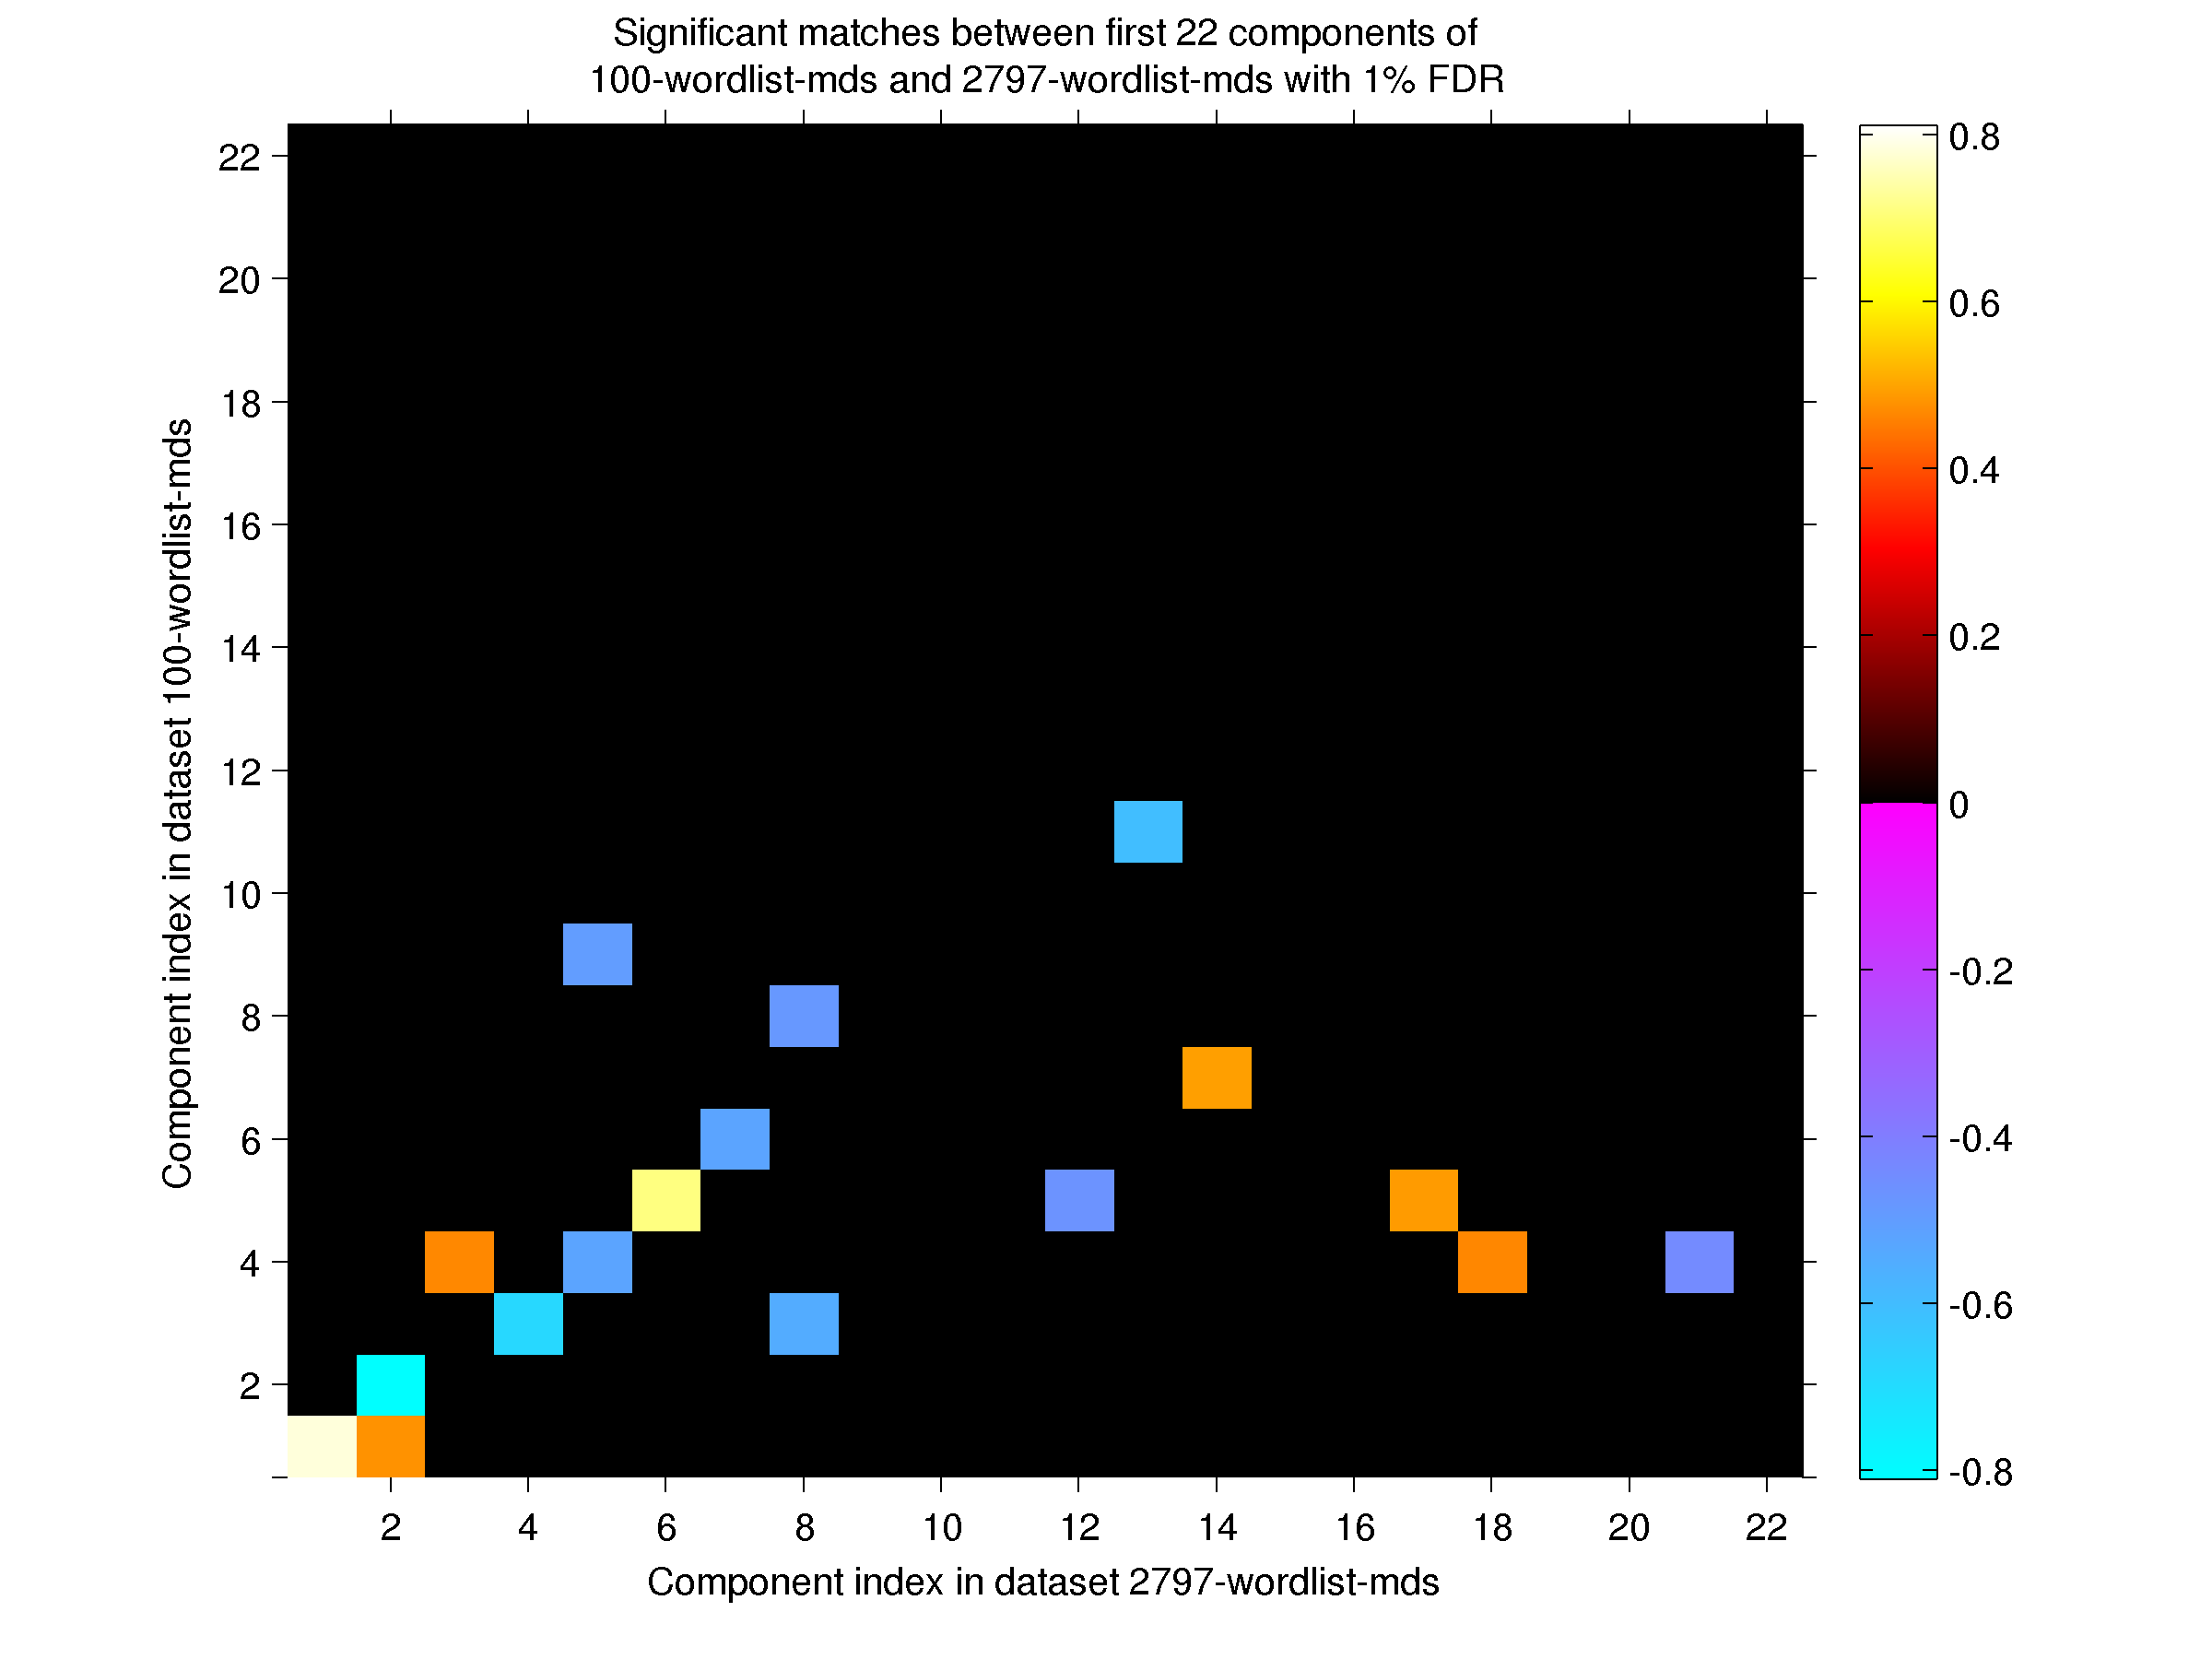
\includegraphics[width=0.9\linewidth]{100-vs-2797-from-800dim-lowercase-wmt-model-significant-first-22}
    \caption{Results from Table 
    \ref{100-vs-2797-from-800dim-lowercase-wmt-model-significant-first-22.tex} 
    displayed as an image. Colors (except black) give correlation for matching 
    dimensions.}
    \label{fig:100vs2797First22}
\end{figure}


\end{document}

\documentclass[eric_thesis.tex]{subfiles}
\begin{document}
\chapter{Discussion}

\section{Interpretation of the dimensions}

As I performed the component extractions, I examined the sorted word-lists, 
which meant that I saw them in approximate numerical order according to the size 
of the list. As I examined the components for the smaller word lists, I had 
trouble coming up with coherent explanations. Some of the first few components 
seemed related to a good/bad trait listing but the rest of the components will 
be difficult to figure out. For example, components 1 and 2 of the unnormalized 
101 word set seem to be more-or-less good/bad. This is a rough characterization. 
Component 1 includes both extroverted and bashful on the ``bad'' side and 
component 2 includes prompt on its bad side. But the rest of the components are 
hard to describe. Even in the smaller lists, the MDS transform makes them much 
more interpretable. In the first two components, there are many fewer strange 
entries at the ends than when using the other two normalization methods. The 
rest of the components are still hard to interpret though this is more from a 
lack of vocabulary than from no sense in the ordering. In hindsight, having seen 
the larger MDS set, it is clear that the third component is sorted on formality 
and the fourth is related to how often the word is used to describe nonhuman 
versus human characteristics. 

\subsection{2797 Word with MDS}

Once I reached the 2797 word list based on \citep{Norman1967}, interpretation 
became much easier. I think more than 14 components might be interpretable, 
however, I only had time for 14. Several of those need some improvement. 
My interpretations are in Table
\ref{tab:2797mdsinterp}.

\subsubsection{Component 1}

The first dimension needs a bit of explanation. In the corpus, the 10 highest 
ranked words appear in 526515/117296559 sentences (0.4\%), the 10 lowest 
ranked words appear in only 5871 (0.005\%). This is even more pronounced in the 
minutes of the European parliament where the highly ranked words appear in 
19196/2015440 sentences (1\%) but the lowest ranked words appear in 14 
(0.0006\%) (And, in all of those sentences, the only word appearing is 
sly\_jj - the highest ranked word among the lowest 10). Thus, it may not be 
just that these words are more common, but that they are more common in 
political speech.

I looked at the Spearman correlation between number of occurrences of the words 
in the entire corpus and the values in on the first dimension. It was 0.5739 
(which gives a p value of $1.9120 \times 10^{-163}$ against the null hypothesis 
that there is no relationship). There is no other component which is so 
strongly correlated with word frequency. However, the correlation is not 
perfect. For example, the most frequent word in the list has a rank of 204 when 
you look at its score on the first dimension.

To investigate the hypothesis that these words are not just more common but 
more common in political speech, I also looked at the correlation with 
frequency in the European parliament records. The correlation goes up to 0.6881 
(p=3.8268e-261) and up to 0.7027 when looking at only words that appear in the 
parliamentary records. That it is not a perfect correlation indicates that 
there are still things I am overlooking. However, describing this dimension as 
``uncommon in parliament vs common'' seems to have some explanatory power.

\begin{table}[tbp]
\begin{tabular}{ | l |p{1.1in}|p{1.1in}|p{1.8in} |}
 \hline
 C & Low & High & Comment \\
 \hline
 1 & Uncommon in parliament & common in parliament & \\
 2 & Negative & Positive & \\
 3 & Mainly describes humans & Describes non-humans also & \\
 4 & Informal & Formal & \\
 5 & Used in conflict & in peace & \\
 6 & Unrelated & Related to patriotism or authority-group loyalty & \\
 7 & Rebellious intellectual stereotype & Stereotypical opponent of 
     rebellious intellectual & \\
 8 & Less emotional words & Emotionally charged words & Some of the low end 
   may be words describing those with less emotion rather than words that 
   stir up less emotion in the hearer\\
 9 & social ostentation & private  & But against this 
       interpretation, fuddy-duddy gets in the low end. Another word
       that doesn't fit well ``cackler'' is very common in news 
       stories about a particular police officer in Dallas whose discipline 
       hearing exposed a scandal in the police force. \\
 10 & business / practicality? & religion / family / clan & \\
 11 & Used to describe people in violent situations & Used to describe people in 
       non-violent situations & \\
 12 & Unknown & restaurant and food (high) & Maybe: world falls apart vs world 
       holds together. (You never see dispiriting, bleak, nagging in a 
       restaurant review or recipe.) \\
 13 & restaurant review & ways people present themselves/words used in describing new 
       people ``Wavy, mousy brown hair '' & \\
 14 & words that can describe both politicians or speeches and food  &  Unknown & \\
 \hline
 \label{tab:2797mdsinterp}
\end{tabular}
\end{table}

\subsection{All combined with MDS}

Here the categories look similar to the 2797 word list. 

\begin{enumerate}
 \item Unknown
 \item Same
 \item Same
 \item Same
 \item Reversed from 2797
 \item Unknown
 \item Words that describe statements and people who make them thereby 
       affecting our interpretation thereof vs unknown
\end{enumerate}

\subsection{2797 with z-score}

These were much harder to interpret and there are more exceptions to each rule. 
This is to be expected from the difference between the dot-product space in 
which the similarity actually is measured and the euclidean space in which the 
z-score and PCA combination operates.

\begin{enumerate}
 \item business (low) \ldots fashion (high)
 \item socially pleasant (low) \ldots socially unpleasant (high) - mostly 
adjectives at the extremes.
 \item leadership qualities (low) vs ?words used in other contexts (words with 
less focus on personality)?
 \item things involving commitment/loyalty/disloyalty vs words that can 
describe art - but against this: ``lucky'' having to do with personality?
\end{enumerate}

\section{Thoughts on interpretations}

It seems that a lot of the dimensions are characteristics of the words 
themselves and not as much characteristics of what the word describes.

MDS is easier to interpret.




\section{Not what I expected}

\section{Could it be the corpus?}

WMT11 is a news corpus. Possibly its topic matter does not focus on people enough for those word senses to be properly represented. There are other, smaller, corpora with much broader language representation - for example, the brown corpus is a well known and freely available million word corpus. The British National Corpus is in the hundreds of millions of words and was created to be very broad-based. Additionally, there are spoken-language corpora like MICASE (Michigan Corpus of Academic Spoken English) and CPSA (Corpus of Spoken Professional American-English). These corpora could be used by themselves or potentially improved by using a model derived from a large news corpus like WMT11 or Gigaword as a starting point and then training on the smaller corpus.

\section{Could it be polysemy?}

\section{Could the dimensions be non-personality attributes?}
\section{Could the dimensions not be scaled on personality-ness?}

\todo{What I mean here is that the dimensions could be things like ``suitability to describe warmth'' both cold and warm would score highly but organized would score low.}

\section{Could the number of dimensions in the lexical model be affecting things?}

\section{Could the personality meanings not be being captured?}

\todo{This may be part of the previous - too few or too many dimensions might elide the personality dimensions}

\section{Could the problem be an underlying nonlinear structure?}

\section{Could the problem be the nonlinear transformation from cosine to Euclidean topology?}

\chapter{Future Work}

\section{Normalize vectors to unit length}

\todo{stub}

Since the cosine distance is the only one with direct semantic weight, I can 
get rid of noise that may be confusing PCA under the other transformations by
normalizing all score vectors to unit length. This leaves the cosine distance
unchanged but should make the Euclidean distance closer to the cosine distance
in those places where it diverges.

Why didn't I do it now? Because I would have had to reinterpret the dimensions.
(Though a dimension mapping from the already interpreted 2797-word list would
work.)

\section{Remove non-human words}

\todo{stub}

One of the dimensions in the 2797 word MDS analysis is a human-nonhuman 
dimension. It may measure to some extent the degree of polysemy of the words. A 
nice analysis would be to just extract the words that scored well on the human 
side of this scale and see what their most important dimensions are. It might 
reduce the noise significantly.

\section{Use directional statistics}

\todo{stub}

One problem with the MDS approach is that I can't standardize the range and 
mean beforehand because taking the z-scores of the dimensions changes the 
angles involved in the dot-products. However, I can map the word vectors to 
the unit sphere without changing the cosine distances. Then directional 
statistics give me analogous measures to the mean and standard deviation. 
Applying MDS to the distances in these standardized points should give me 
something much closer to the factor analysis normally used in psychology.

\todo{If I finish all sections but the discussion, I can try using directional 
stats to normalize the vectors before applying MDS}

\section{Rerun on other corpora or different random subsets of the same corpus}

\todo{Those factors that are stable can be assumed to be represent actual characteristics of language in general and not noise fitted by the algorithm in the particular corpus}

\subsection{Gigaword}
\subsection{Project Gutenberg}
\subsection{Smaller corpora}
\subsection{Small corpus from large starting point}

\section{Examine technique for detecting word usage shift between corpora}

\todo{Turn text summary of method below into more final version for future work}
Train model 1 on corpus 1. Save model 1. Train model 2 on corpus 2 using model 1 as a starting point. Align the two models (using words common to the two corpora and a loss function that depends on how many different words you expect (for example, if you will use $L^p$ norms\footnote{An $L^p$ norm calculates the length of an n-dimensional vector $x$ as $\|x\|_p=\left(|x_1|^p+|x_2|^p+\dotsb+|x_n|^p\right)^{\frac{1}{p}}$} and subtraction to calculate distance, you can use a lower $p$ exponent for a lower proportion of expected differences).

\section{Perform modeling in Euclidean topology}

\todo{Turn summary into final form}
Because the vectors must be converted to use Euclidean distances before PCA will work correctly, the principal components are not components of the vectors in cosine distance space. Thus, I can only rank the personality words and it is impossible to look for dimensions whose meaning will not be obvious based on ranking the personality words.

One approach would be to transform all the words. However the distance matrix alone would be enormous (5 hundred thousand words would require 250 billion distances). Since most modern MDS implementations use some form of gradient descent under the hood, I considered using stochastic gradient descent with the distance matrix being implicit in the original point values. The initial point for the descent could be the original point values since Euclidean and cosine distances are similar. However, that is a very special-purpose application of MDS. Since it could be hard to code due to the sizes of the data involved, and would only give an approximation of the best point locations, I don't think it is worth the effort at this time.

I think it is better to rewrite the training section of the skip-gram to use Euclidean rather than cosine distance. This modification will increase training time by a constant factor, but I would hope that factor is small.

\section{Do the big-5 etc. personality dimensions come out of a pseudo-personality test?}
\todo{Turn summary into final form}
What I mean is if you count the frequency for which different personality adjectives are used to describe different named person-entities in the corpus, do you get the same descriptive dimensions as you do for when you ask people to rate others on n dimensions.

\section{What happens if you tag personality words when they are referring to a specific person?}

\section{Use perplexity to calculate the number of personality dimensions}

\section{Use varimax rotation}

\todo{turn summary into final form} 

This might or might not be worthwhile. On the one hand, maybe the way
psychologists do it will produce the same result. On the other hand,
Goldberg \todo{cite ref goldberg 1990 An alternative ``Description of
  Personality''} found the same 5 factors using both common factor
analysis and principal components and both orthogonal and oblique
rotation.

\end{document}


\documentclass[eric_thesis.tex]{subfiles}
\begin{document}
\appendix
\chapter{Scripts used in preprocessing}
\section{Text of filter\_angle\_tags.pl}
\label{app:filterangletags}
\lstset{language=Perl}
\begin{lstlisting}
#!/usr/bin/perl
use strict;
use warnings;

#######################
# Usage: filter_angle_tags.pl < source > dest
# or:    filter_angle_tags.pl source1 source2 > filtered
#
# Remove stray html, urls and stock symbols to prepare
# for tagging

my $has_bracket_pair = qr!<[A-z/][^<>]*>!;
my $bracket_pair_split = qr!($has_bracket_pair)!;
my $html_string = q(<span |<strong>|</strong>|).
    q(<em>|</em>|<[bauipq]>|</[pqbaui]>|<\s*br\s*/?>|).
    q(<\s*/br\s*>|<p\s*/?>|</?h.>|</?blockquote|).
    q(</?code>|<font[ >]|</font|</?acronym|</?strike|).
    q(</?cite|</?q |</>|</?abbr |</?del |<javascript|).
    q(</?itals>|</?script|</?center>|<SPEAKER );
my $html_regex = qr(${html_string});

sub keep_segment{
    my ($seg) = @_;
    return !($seg =~ m!$has_bracket_pair!) or !(
        $seg =~ m(http://) or
        $seg =~ m(href) or
        $seg =~ m(\.com\W|\.gov\W) or
        $seg =~ m(${html_regex}) or
        $seg =~ m(<[A-z0-9]{0,9}[.=/][A-Z0-9]{0,6}>) or
        $seg =~ m(<CF7[01]>) or
        $seg =~ m(<ID:[A-z0-9]+>)
        );
}

while(<>){
    chomp;
    if (m/$has_bracket_pair/) {
        my @segments = split($bracket_pair_split, $_);
        @segments = grep( &keep_segment($_), 
                          @segments);
        print join(" ", @segments),"\n" 
            if (@segments);
    }else{
        print "$_\n";
    }

}
\end{lstlisting}

\section{Text of tag\_corpus.sh}
\label{app:tagcorpus}
\lstset{language=sh}
\begin{lstlisting}
#!/bin/bash

############
# Script I used to tag the WMT11 corpus - it needed to
# be split because the TreeTagger tokenizer reads
# everything into memory.

# The data file for the cleaned data
WMT11=/mnt/linux_data/wmt11_no_angle_tags.txt

# The prefix used for split files
SPLIT_FILENAME=/mnt/linux_data/wmt11_no_angle_split

# Data file for the tagged data
TAGGED_WMT11=/mnt/linux_data/wmt11_tagged.txt

# Put treetagger on path
PATH="$PATH:/home/eric/SW/TreeTagger/cmd:"\
"/home/eric/SW/TreeTagger/bin:."

# Split into 10,000,000 lines per file (about 1.5GiB
# per)
if [ -f ${SPLIT_FILENAME}aa ]; then 
    echo "Not splitting again. Split already exists"
else
    split -l10000000 "$WMT11" "$SPLIT_FILENAME"
fi

# Tag the split files
if [ -f "$TAGGED_WMT11" ]; then 
    echo "Not tagging again. Tagged file "\
         "already exists"
else
    for i in ${SPLIT_FILENAME}*; do
        echo "Tagging $i"
        tree-tagger-english-utf8 $i | \
            reassemble_tags.pl >> "$TAGGED_WMT11"
    done
fi
\end{lstlisting}

\section{Text of tag\_word\_list.pl}
\label{app:tagwordlist}
\lstset{language=Perl}
\begin{lstlisting}
#!/usr/bin/perl
use strict;
use warnings;
use HotKey;
use URI::Escape;
use File::Fetch;

#
# Reads a word-list from a file (DON'T USE STDIN, it
# mistakes it for keyboard input). For each word,
# displays the word-net entry web-page in firefox and
# then asks if it is a valid as a personality
# adjective. Next it asks if it is valid as a
# personality non-adjective. If it was a valid
# adjective, it writes word_jj to stdout. If it was a
# valid non-adjective, it writes word to stdout.  If
# you type q at any prompt, it exits, writing "THERE
# WAS A PROBLEM" to stdout.
#
# Using the assumption that every word in the file is a
# personality word, does the disambiguation itself if
# the word has only one part of speech. (However, this
# code depends on the format of the html returned and
# so is fragile.)
#
# Prompts are written to stderr (which is fine on
# Linux, but probably a mess under Windows)

sub getynq {
    my $key = readkey();
    while($key =~ m/^[^ynq]$/){
        print STDERR "\nPlease enter y,n, or q.";
        $key = readkey();
    }
    return $key;
}

WORD: while(<>){
    chomp;

    my $query_uri =
        'http://wordnetweb.princeton.edu/perl/webwn?s='.
        uri_escape($_).
        '&sub=Search+WordNet&o2=&o0=1'.
        '&o7=&o5=&o1=1&o6=&o4=&o3=&h=';
    # Try automatic determination - if there is only
    # one level three header (used to contain the part
    # of speech) then if it is "Adjective" the word is
    # a personality adjective. Otherwise, the word is a
    # personality non-adjective. Ignore verb and adverb
    # meanings because I am looking for words about
    # personal qualities. I want "The brave man" or "he
    # had courage" and not "He will brave the elements"
    # or "Home of the brave".
    #
    # With the 2797 word list, I have decided to accept
    # words that are categories - like "the home of the
    # brave."
    my $contents;
    my $fetcher = File::Fetch->new(uri => $query_uri);
    $fetcher->fetch(to => \$contents);

    my @level_3_headers = ($contents =~
                         m:<h3>[^<]+</h3>:gi);

    @level_3_headers = # Remove verbs
        grep{!m:<h3>Verb</h3>:} @level_3_headers; 
    @level_3_headers = # Remove adverbs
        grep{!m:<h3>Adverb</h3>:} @level_3_headers; 

    my $autotag_successful = 0;
    if (@level_3_headers == 1){
        # If the only part of speech is adjective tag
        # as such, otherwise if the only part of speech
        # is noun, tag as non-adjective. If the part of
        # speech is something else (an unknown part of
        # speech or an error message) don't tag and
        # leave it to the humans.
        if($level_3_headers[0] =~ 
              m:<h3>Adjective</h3>:i){
            print STDOUT "${_}_jj\n";
            $autotag_successful = 1;
        }elsif($level_3_headers[0] =~ 
              m:<h3>Noun</h3>:i){
            print STDOUT "${_}\n";
            $autotag_successful = 1;
        }else{
            $autotag_successful = 0;
        }
    }
    if ($autotag_successful){
        # We've tagged the word. Read the next word
        print STDERR "Automatically ",
                     "determined ${_}.\n";
        next WORD;
    }


    # Manual determination - open firefox (ignoring
    # error messages) and ask the user

    system("firefox \"".
           "$query_uri\" > /dev/null 2>&1 &");

    my $had_to_do_with_personality=0;
    print STDERR "\nIs $_ a valid personality ".
        "adjective? (yes/no/quit)";
    my $key = getynq();
    if($key =~ m/y/i){
        print STDOUT "${_}_jj\n";
        $had_to_do_with_personality = 1;
    }elsif($key =~ m/q/i){
        print STDOUT "THERE WAS A PROBLEM\n";
        exit(-1);
    }

    print STDERR "\nIs $_ a valid personality ",
        "quality or type of person ('His ",
        "characteristic $_' or 'The $_ is ",
        "characterized ",
        "by $_-ness')? Only accept for type of ",
        "person if ",
        "the word is not an adjective or a much more ",
        "common usage than the adjective. (braggart, ",
        "for ",
        "example, has an archaic adjectival use but ",
        "is ",
        "much more commonly used as a ",
        "category)(yes/no/quit)"; 
    $key = getynq();
    if($key =~ m/y/i){ 
        print STDOUT "${_}\n";
        $had_to_do_with_personality = 1; 
    }elsif($key =~ m/q/i){ 
        print STDOUT "THERE WAS A PROBLEM\n";
        exit(-1); 
    }

    unless($had_to_do_with_personality){
        print STDERR "\n$_ must have something to ",
             "do with personality. You can't ",
             "answer n on both questions.\n";
        print STDOUT "THERE WAS A PROBLEM\n";
        exit(-1);
    }
} 
\end{lstlisting}


\section{Text of reassemble\_tags.pl}
\label{app:reassembletags}
\lstset{language=Perl}
\begin{lstlisting}
#!/usr/bin/perl
use strict;
use warnings;

################
# Usage: reassemble_tags.pl < tagged.txt
#
# Takes tagged text from treetagger and reassembles it
# into 1 sentence per line (multiple sentence ending
# tags are kept on the same line)

# Tracks whether the previous tag was a sentence-ender
# in order to tell where to end the lines.
my $last_tag_was_sentence=(1==0);

# Combine words and sentences
while(<>){
    my ($word, $tag) = split('\t');
    if(defined($tag)){
        # End the line if transitioning from "SENT" to
        # another tag
        my $tag_is_sentence = $tag eq "SENT";
        if ($last_tag_was_sentence && !$tag_is_sentence){
            print "\n";
        }

        # Output the word with its tag
        if(defined($word)){
            print "${word}_${tag} ";
        }else{
            print "${word}_unknown_tag ";
        }

        # Update last tag state variable
        $last_tag_was_sentence = $tag_is_sentence;
    }
}

# If the last tag in the file was a sentence tag,
# output a newline
if ($last_tag_was_sentence){
    print "\n";
}
\end{lstlisting}

\chapter{Scripts used in analysis}

\section{extract\_vectors.py}
\label{app:extractvectors}
\lstset{language=Python}
\begin{lstlisting}
#!/usr/bin/python
from gensim.models import word2vec
import logging
import os
import csv
import sys


# Check command line arguments and print usage if
# wrong number of arguments
if len(sys.argv) != 3:
    import textwrap
    sys.stderr.write(
        "Usage: %s list_of_terms.txt "+
        "model_file.model\n" % sys.argv[0])
    sys.stderr.write("\n")
    sys.stderr.write(
        textwrap.fill(
            "Each line in list_of_terms.txt is "+
            "treated as a term. For each term, if a "+
            "corresponding term exists in the "+
            "word2vec model (generated by "+
            "word2vec.save) then that term and the "+
            "corresponding vector are printed to "+
            "stdout as a csv file"))
    sys.exit(-1)

# Command line arguments
term_list_filename = sys.argv[1]
input_model_filename = sys.argv[2]

# Set up logging
logging.basicConfig(
    format='%(asctime)s : %(levelname)s : %(message)s', 
    level=logging.INFO)

# Load the model
model = word2vec.Word2Vec.load(input_model_filename)
logging.info("Done loading input model")

# Loop through the terms, outputting appropriate
# vectors
out = csv.writer(sys.stdout)
with open(term_list_filename) as terms:
    for term in terms:
        try:
            term = term.rstrip() # Remove line-ending
            v = model.vocab[term]
            vector = model.syn0[v.index]
            vector_str = ["%.19g" % n for n in vector]
            out.writerow([term] + vector_str)
        except KeyError:
            logging.info('Skipped missing term "%s"' % 
                         term)
\end{lstlisting}


\section{Elbow point algorithms}
\label{app:elbow_point_algorithms}
\lstset{language=Matlab}

\subsection{elbow\_point.m}

\begin{lstlisting}
 function [elbow_index,best_estimate] = ...
      elbow_point(lambdas)
% Returns the index at which the slope of the lambdas
% changes
%
% In using a scree plot to discover the number of 
% principal components, a frequent method is to choose
% the "elbow", the inflection point of the curve. One
% way of formalizing this is approximating the scree 
% plot with two lines. One goes from the  beginning to
% the elbow point and the other to the end. Whichever
% is closest is the best elbow point 
%
% Exhaustive search for the best approximation of
% the function composed of the ordered pairs
% i,lambdas(i) composed of the lines
% (1,lambdas(1))...(i,lambdas(i)) and
% ((i,lambdas(i)...(end, lambdas(end))
%
% Mean absolute value of the difference is used as
% the measure of goodness of fit
%
% best_estimate - the linear fit to the lambdas
% implied by elbow_index

if size(lambdas,1) > 1
    lambdas = lambdas';
end
best = 1;
best_error = inf;
best_estimate = [];
for cur=1:length(lambdas)
    cur_estimate_a = linspace(lambdas(1), ...
         lambdas(cur), cur);
    cur_estimate_b = linspace(lambdas(cur), ...
         lambdas(end), length(lambdas)-cur+1);
    cur_estimate = [cur_estimate_a(1:end-1), ...
         cur_estimate_b];
    cur_error=mean(abs(cur_estimate - lambdas));
    if cur_error < best_error
        best_error = cur_error;
        best = cur;
        best_estimate = cur_estimate;
    end
end

elbow_index = best;

end
\end{lstlisting}

\subsection{flex\_end\_elbow\_point.m}
\begin{lstlisting}
 function [elbow_index,best_estimate] = ...
      flex_end_elbow_point(lambdas)
% Returns the index at which the slope of the lambdas
% changes
%
% In using a scree plot to discover the number of
% principal components, a frequent method is to
% choose the "elbow", the inflection point of the
% curve. One way of formalizing this is approximating
% the scree plot with two lines. One goes from the
% beginning to the elbow point and the other to the
% end. Whichever is closest is the best elbow point.
%
% This code is similar to elbow_point except that the
% height at the ends is adjustable. This frequently
% leads to a more conservative estimate of when the
% slope changes and a closer approximation of the
% lambdas. I think it is more like what humans do than
% offset_elbow_point.
%
% Exhaustive search for the best approximation of the
% function composed of the ordered pairs i,lambdas(i)
% composed of the lines (1,height_1)...(i,lambdas(i))
% and ((i,lambdas(i)...(end, height_end)
%
% Mean squared difference is used as the measure of
% goodness of fit. (It looks more like what a human
% would do than the mean abs used in other
% elbow_point versions.)
%
% best_estimate - the linear fit to the lambdas
% implied by elbow_index

if size(lambdas,1) > 1
    lambdas = lambdas';
end
best = 1;
best_error = inf;
best_estimate = [];
for cur=1:length(lambdas)
    % Since the two lines are independent, we can
    % minimize them in sequence. I minimize the error
    % on the first line, holding the second constant
    % then minimize the second line holding the first
    % at the optimum found in the first pass
    [h1, ~]=fminbnd(@(h) linpredict([h,lambdas(end)]),...
         lambdas(cur), max(lambdas));
    [~, cur_error]=fminbnd(@(h) linpredict([h1,h]),...
         -max(lambdas), lambdas(cur));
    if cur_error < best_error
        best_error = cur_error;
        best = cur;
        best_estimate = cur_estimate;
    end
end

elbow_index = best;

    % Calculate the two-line fit with the elbow_index
    % at cur and the heights at the beginning and end
    % set to heights(1) and heights(2) Also sets
    % cur_estimate and uses lambdas
    function err=linpredict(heights)
        cur_estimate_a = linspace(heights(1),...
             lambdas(cur), cur);
        cur_estimate_b = linspace(lambdas(cur), ...
             heights(2), length(lambdas)-cur+1);
        cur_estimate = [cur_estimate_a(1:end-1),...
             cur_estimate_b];
        err=mean(abs(cur_estimate - lambdas).^2);
    end

end
\end{lstlisting}

\subsection{log\_scree\_elbow.m}
\begin{lstlisting}
function [elbow_index,best_x1, best_x2, predicted] = ...
     log_scree_elbow( lambdas, min_dist )
% Looks for the line in the log(lambdas) that has the
% most inliers, then counts the first outlier as the
% elbow
%
% Scree plots of random stuff look like exponential
% curves. Thus, they are flat on a log scale. The
% dimensions carrying information either have a
% different slope or aren't exponential at all. Thus,
% they will be outliers. On a log plot, the random
% stuff looks like a straight line. (However, if
% the system is rank deficient, the last few principal
% components will sharply trail off and not look like
% a straight line.)
% 
% Let lambdas be the 'latent' return from princomp.
% 
% I fit an exponential to the end-points of all
% sufficiently large sub-intervals of the lambda
% values. I choose the interval whose error looks the
% most like Gaussian noise (that is, has the lowest
% test statistic for a Jarque-Bera). Then I fit an
% exponential to all those points and calculate the
% standard deviation of the errors. Finally, the
% first point with an error less than 3 standard
% deviations, I count as the first random point. All
% points before that are outliers and I count the
% last of the outlier points as my elbow index.
%
% lambdas - a vector of strictly postitive scalars
%     sorted in decreasing order. The 'latent'
%     return from princomp
%
% min_dist - the minimum length interval to be
%     considered as a potential "all-random" interval.
%     The smaller this is, the less power the
%     normality test has. However, it cannot be larger
%     than the number of random values that are
%     decreasing exponentially. The default is
%     length(lambdas)/4

if any(lambdas <= 0)
    error('log_scree_elbow:pos_lambda',...
        ['All lambda values must be strictly '...
        'positive in log_scree_elbow']);
end

if ~exist('min_dist','var')
    min_dist = ceil(length(lambdas)/4);
end

if min_dist < 2
    error('log_scree_elbow:min_dist_too_small',...
        ['min_dist parameter to log_scree_elbow '...
        'must be at least 2.']);
end
        

if length(lambdas)-min_dist < 20 % This is a fudge
                  % factor, but if it is less than 
                  % 20, there are way too few points
    error('log_scree_elbow:not_enough_points',...
        ['There must be at least 20 more lambda '...
        'values than min distance']);
end

if size(lambdas, 1) > 1
    lambdas = lambdas';
end

% Loop two indices x1 and x2 through the lambdas,
% fitting an exponential and finding outliers
n=length(lambdas);
best_x1 = 1;
best_x2 = 1+min_dist;
best_normality_test_stat = inf;
warning('off','stats:jbtest:PTooBig');
warning('off','stats:jbtest:PTooSmall');
for x1=1:n
    y1=lambdas(x1);
    for x2=(x1+min_dist+1):n
        % Fit an exponential to these two points
        y2=lambdas(x2);
        b=(-log(y1)+log(y2))/(-x1+x2);
        a=y1/exp(b*x1);

        % Calculate the errors for that exponential
        predicted=a.*exp(b.*(1:n));
        errors = lambdas-predicted;

        % Calculate the degree to which the errors in
        % that interval match the normal distribution.
        % Ideally, I'd use the Anderson-Darling test
        % statistic because I am particularly
        % interested in excluding outliers from the
        % interval and it is more sensitive to them.
        % However, it is not available in R2012, so
        % I will use the Jauques-Berra test
        is_inlier = (1:n > x1) & (1:n < x2);
        [~,~,jbtest_stat]=jbtest(errors(is_inlier));
        inlier_std = std(errors(is_inlier));
        if isnan(inlier_std)
            fprintf('Nan');
        end
        % If this section looks more normal than any
        % others, call it the best
        if jbtest_stat < best_normality_test_stat
            best_normality_test_stat = jbtest_stat;
            best_x1 = x1;
            best_x2 = x2;
        end
    end
end
warning('on','stats:jbtest:PTooSmall');
warning('on','stats:jbtest:PTooBig');


% Do a least-squares fit on all the inliers
x1 = best_x1;
x2 = best_x2;
y1=lambdas(x1);
y2=lambdas(x2);
b=(-log(y1)+log(y2))/(-x1+x2);
a=y1/exp(b*x1);
is_inlier = (1:n > x1) & (1:n < x2);

xdata = find(is_inlier);
ydata = lambdas(is_inlier);
inlier_params = nlinfit(xdata, ydata, @expfun, [a,b]);

% Calculate the errors for that exponential
predicted=inlier_params(1).*exp(inlier_params(2).*(1:n));
errors = abs(lambdas-predicted);

% Calculate the standard deviation on the points in
% the interval between the two best points
between_std = std(errors(best_x1+1:best_x2-1));

% Outliers are those that are more than 3 std away
is_inlier = errors <= 3*between_std;

% The outlier before the first inlier is our elbow
elbow_index = find(is_inlier,1,'first');
if elbow_index > 1
    elbow_index = elbow_index - 1;
end

% 
% Helper function for fitting
    function predicted = expfun(params, x)
        A = params(1);
        B = params(2);
        predicted = A .* exp(B .* x);
    end

end
\end{lstlisting}

\subsection{offset\_elbow\_point.m}
\begin{lstlisting}
function [elbow_index,best_estimate] = ...
     offset_elbow_point(lambdas)
% Returns the index at which the slope of the lambdas 
% changes
%
% In using a scree plot to discover the number of 
% principal components, a frequent method is to choose
% the "elbow", the inflection point of the curve. One
% way of formalizing this is approximating the scree 
% plot with two lines. One goes from the beginning to
% the elbow point and the other to the end. Whichever
% is closest is the best elbow point.
%
% This is similar to elbow_point except that the
% height at the joining of the two lines is not one
% of the lambdas. This frequently leads to a more
% conservative estimate of when the slope changes and
% a closer approximation of the lambdas.
%
% Exhaustive search for the best approximation of the
% function composed of the ordered pairs i,lambdas(i) 
% composed of the lines (1,lambdas(1))...(i,height)
% and ((i,height...(end, lambdas(end))
%
% Mean absolute value of the difference is used as
% the measure of goodness of fit
%
% best_estimate - the linear fit to the lambdas
%     implied by elbow_index

if size(lambdas,1) > 1
    lambdas = lambdas';
end
best = 1;
best_error = inf;
best_estimate = [];
for cur=1:length(lambdas)
    [~, cur_error]=fminbnd(@linpredict, min(lambdas),...
         max(lambdas));
    if cur_error < best_error
        best_error = cur_error;
        best = cur;
        best_estimate = cur_estimate;
    end
end

elbow_index = best;

    % Calculate the two-line fit with the elbow_index
    % at cur and the height at the elbow set to
    % height. Also sets cur_estimate and uses lambdas
    function err=linpredict(height)
        cur_estimate_a = linspace(lambdas(1), ...
            height, cur);
        cur_estimate_b = linspace(height, ...
            lambdas(end), length(lambdas)-cur+1);
        cur_estimate = [cur_estimate_a(1:end-1), ...
            cur_estimate_b];
        err=mean(abs(cur_estimate - lambdas));
    end

end
\end{lstlisting}

\subsection{scree\_elbow\_using\_robust\_fit.m}
\begin{lstlisting}
function [elbow_index,best_x1, best_x2, ...
     minified_ranks, predicted, ranks] = ...
     scree_elbow_using_robust_fit( lambdas, ...
          error_prctile )
% Looks for the line in the log(lambdas) that has the
% most inliers, then counts the first outlier as the
% elbow
%
% Scree plots of random stuff look like exponential
% curves. Thus, they are flat on a log scale. The
% dimensions carrying information either have a
% different slope or aren't exponential at all. Thus,
% they will be outliers. On a log plot, the random
% stuff looks like a straight line. (However, if the
% system is rank deficient, the last few principal
% components will sharply trail off and not look like
% a straight line.)
% 
% Let lambdas be the 'latent' return from princomp.
% Treat error_prctile like it was a fraction.
% 
% I robustly fit an exponential to the whole curve.
% Then I choose error_prctile of the best errors and
% robustly fit the exponential again to the interval
% containing those points. Finally, I choose the
% interval containing error_prctile of the best points
% again and use that interval as the interval of
% random points. The point before the first point in
% the interval is the elbow index - the first
% non-random lambda.
%
%
%
% INPUT:
%
% lambdas - a vector of strictly postitive scalars 
%     sorted in decreasing order. The 'latent' return
%     from princomp
%
% error_prctile - a scalar from 0..100. The points
%     with an error less than error prctile are used
%     to create the region from which the exponential
%     fit is calculated. Default is 25, so the top 25%
%     of the errors are used. The smaller 
%     error_prctile the smaller the sample used to 
%     estimate the equation governing noise lambdas.
%     So, you'd like error_prctile to be large. 
%     However, if error_prctile is too large then the
%     size of the non-random interval will be
%     overestimated.
%
%
%
% OUTPUT:
%
% elbow_index - the index of the last of the 
%     non-random lambdas
%
% best_x1 - the first index of the random lambda 
%     interval
%
% best_x2 - the last index of the random lambda 
%     interval
%
% minified_ranks - minified_ranks(i)=min(ranks(1:i)).
%     100*minified_ranks(i)/max(ranks(i)) can be
%     thought of a number p such that if 
%     error_prctile > p, then i will be best_x1. If
%     error_prctile were not used twice, this would be
%     the definition. However, there is some minor
%     interaction with error_prctile that makes this
%     only approximate.
%
% predicted - the exponential function that was
%     fitted to the random values
%
% ranks - rank(i) is the rank of the error when
%     estimating lambdas(i) with predicted(i). The
%     smallest errors have the smallest ranks.
%

if any(lambdas <= 0)
    error('scree_elbow_using_robust_fit:pos_lambda',...
        ['All lambda values must be strictly ' ...
        'positive in scree_elbow_using_robust_fit']);
end

if ~exist('error_prctile','var')
    error_prctile = 25;
end

num_points = floor(length(lambdas)*error_prctile/100);

if num_points < 2
    error(['scree_elbow_using_robust_fit:'...
        'num_points_too_small'],...
        ['When error_prctile points are selected '...
        'from lambdas in '...
        'scree_elbow_using_robust_fit there must '...
        'be at least 2.']);
end

if size(lambdas, 1) > 1
    lambdas = lambdas';
end


% Find a starting point for an exponential fit to
% the whole line. Here I do a linear fit to the
% logarithm.
n=length(lambdas);
warning('off','stats:statrobustfit:IterationLimit');
robust_params = robustfit(1:n, log(lambdas));
warning('on','stats:statrobustfit:IterationLimit');

% Next, I use the linear robust fit as the starting
% point to do a nonlinear robust fit on the whole
% line using an exponential function. This should
% be the same, except for the errors being of a more
% appropriate distribution. In particular, I hope that
% the errors in the exponential section are normal
expfun=@(param,x) param(1).*exp(param(2).*x);
fitopts=statset('Robust','on','MaxIter',5000);
starting_pt = [exp(robust_params(1)),...
    robust_params(2)]; % exp(mx+b)=exp(b)*exp(mx)
robust_params=nlinfit(1:n,lambdas(1:n),expfun,...
    starting_pt, fitopts);

% Next, I calculate the inliers. This will help take
% care of the fact that the m-estimators used in
% Matlab's robust fitting still have a zero
% breakdown point.
%
% I find the points with the best error. Then the
% in-lying region is the smallest region that contains
% those points. error_prctile is the fraction of the
% points that are used.
predicted = expfun(robust_params, 1:n);
errors = abs(lambdas - predicted);
max_error = prctile(errors, error_prctile);
best_x1 = find(errors <= max_error, 1, 'first');
best_x2 = find(errors <= max_error, 1, 'last');

% Repeat the estimation in untransformed space using
% only the in-lying points. 
starting_pt = [robust_params(1),robust_params(2)];
robust_params=nlinfit(best_x1:best_x2,...
    lambdas(best_x1:best_x2),expfun,...
    starting_pt, fitopts);
predicted = expfun(robust_params, 1:n);

% Find the in-lying region for the new points. This
% will be the region of random points and the first
% point before it will be our elbow point
errors = abs(lambdas - predicted);
max_error = prctile(errors, error_prctile);
best_x1 = find(errors <= max_error, 1, 'first');
best_x2 = find(errors <= max_error, 1, 'last');

ranks = tiedrank(errors);

% Create a diagnostic based on the ranks of the
% errors. If you divide minified_ranks by 
% length(lambda), you will get the percentile of the
% population you would have needed to choose in order
% for that to be the first in-lying point
minified_ranks = ranks;
for i=2:length(ranks)
    minified_ranks(i)=min(minified_ranks(i-1), ...
        minified_ranks(i)); 
end


if best_x1 > 1
    elbow_index = best_x1 - 1;
else
    elbow_index = 1;
end

end
\end{lstlisting}

\chapter{Ranked word lists}
\label{app:rankedwordlists}
For each list of word vectors, the derived principal components can be used to 
give a numerical score to each word in the list. The following sections list
the most important components derived from each method of analyzing each list.

\section{101 word list}
\subsection{Unnormalized PCA}
\todo{fix what happens with negative scores and ensure that the first digit is correct}
\todo{make the tables two columns so they fit on one page and I don't need to use longtable}
\todo{allow regeneration of tex tables without regenerating PCA/MDS coefficients}
\todo{only print first 15 tables}
\label{app:rankedwordlists:101words:unnormalized}
\begin{longtable}[!htbp]{| rlr@{.}l |}
    \hline
    \textbf{Rank} & \textbf{Word} & \multicolumn[2]{c|}{\textbf{Score}} \\
    \hline
    \endhead
    1 & irritable\_jj & -1 & -5886 \\
    2 & self-pitying\_jj & -1 & -5705 \\
    3 & extroverted\_jj & -1 & -5033 \\
    4 & talkative\_jj & -1 & -4127 \\
    5 & unintelligent\_jj & -1 & -3818 \\
    6 & uncooperative\_jj & -1 & -2884 \\
    7 & rude\_jj & -1 & -2600 \\
    8 & unkind\_jj & -1 & -1717 \\
    9 & bashful\_jj & -1 & -1495 \\
    10 & uncharitable\_jj & -1 & -839 \\
    11 & envious\_jj & -1 & -807 \\
    12 & introspective\_jj & -1 & -655 \\
    13 & selfish\_jj & -1 & -508 \\
    14 & considerate\_jj & -1 & -475 \\
    15 & withdrawn\_jj & -1 & -229 \\
    16 & high-strung\_jj & -1 & -219 \\
    17 & jealous\_jj & 0 & -9988 \\
    18 & insecure\_jj & 0 & -9076 \\
    19 & distrustful\_jj & 0 & -8705 \\
    20 & unsympathetic\_jj & 0 & -8481 \\
    21 & kind\_jj & 0 & -8353 \\
    22 & unemotional\_jj & 0 & -8087 \\
    23 & unsophisticated\_jj & 0 & -6918 \\
    24 & fretful\_jj & 0 & -6844 \\
    25 & unreflective\_jj & 0 & -6163 \\
    26 & moody\_jj & 0 & -6077 \\
    27 & temperamental\_jj & 0 & -5431 \\
    28 & unadventurous\_jj & 0 & -5036 \\
    29 & unimaginative\_jj & 0 & -4083 \\
    30 & agreeable\_jj & 0 & -3564 \\
    61 & harsh\_jj & 0 & 5260 \\
    62 & shallow\_jj & 0 & 5321 \\
    63 & active\_jj & 0 & 5358 \\
    64 & artistic\_jj & 0 & 5453 \\
    65 & inefficient\_jj & 0 & 5701 \\
    66 & haphazard\_jj & 0 & 5841 \\
    67 & cold\_jj & 0 & 5942 \\
    68 & inconsistent\_jj & 0 & 6448 \\
    69 & intellectual\_jj & 0 & 6829 \\
    70 & sloppy\_jj & 0 & 7018 \\
    71 & deep\_jj & 0 & 7727 \\
    72 & cooperative\_jj & 0 & 7826 \\
    73 & bold\_jj & 0 & 8169 \\
    74 & creative\_jj & 0 & 8271 \\
    75 & careful\_jj & 0 & 8584 \\
    76 & warm\_jj & 0 & 8613 \\
    77 & helpful\_jj & 0 & 8729 \\
    78 & neat\_jj & 0 & 8995 \\
    79 & complex\_jj & 0 & 9786 \\
    80 & steady\_jj & 0 & 9945 \\
    81 & organized\_jj & 1 & 125 \\
    82 & practical\_jj & 1 & 305 \\
    83 & vigorous\_jj & 1 & 425 \\
    84 & negligent\_jj & 1 & 606 \\
    85 & simple\_jj & 1 & 1041 \\
    86 & innovative\_jj & 1 & 1617 \\
    87 & systematic\_jj & 1 & 2588 \\
    88 & efficient\_jj & 1 & 3437 \\
    89 & prompt\_jj & 1 & 5582 \\
    90 & thorough\_jj & 1 & 5744 \\
    \hline
    \caption{Scores and rankings for most extreme 30 words in component \#1} \\
\end{longtable}
\begin{longtable}[!htbp]{| rlr@{.}l |}
    \hline
    \textbf{Rank} & \textbf{Word} & \multicolumn[2]{c|}{\textbf{Score}} \\
    \hline
    \endhead
    1 & uncooperative\_jj & -1 & -9476 \\
    2 & negligent\_jj & -1 & -2860 \\
    3 & prompt\_jj & 0 & -9101 \\
    4 & distrustful\_jj & 0 & -7927 \\
    5 & insecure\_jj & 0 & -7198 \\
    6 & inconsistent\_jj & 0 & -7036 \\
    7 & rude\_jj & 0 & -6212 \\
    8 & systematic\_jj & 0 & -6061 \\
    9 & fearful\_jj & 0 & -5728 \\
    10 & impractical\_jj & 0 & -5708 \\
    11 & inefficient\_jj & 0 & -5547 \\
    12 & unsophisticated\_jj & 0 & -5494 \\
    13 & selfish\_jj & 0 & -4869 \\
    14 & unsympathetic\_jj & 0 & -4856 \\
    15 & unintelligent\_jj & 0 & -4842 \\
    16 & careless\_jj & 0 & -4728 \\
    17 & sloppy\_jj & 0 & -4204 \\
    18 & cooperative\_jj & 0 & -3703 \\
    19 & touchy\_jj & 0 & -3605 \\
    20 & withdrawn\_jj & 0 & -3538 \\
    21 & jealous\_jj & 0 & -3474 \\
    22 & irritable\_jj & 0 & -3454 \\
    23 & helpful\_jj & 0 & -3255 \\
    24 & harsh\_jj & 0 & -3029 \\
    25 & undependable\_jj & 0 & -2797 \\
    26 & thorough\_jj & 0 & -2694 \\
    27 & unsystematic\_jj & 0 & -2531 \\
    28 & timid\_jj & 0 & -2525 \\
    29 & unrestrained\_jj & 0 & -2523 \\
    30 & haphazard\_jj & 0 & -2444 \\
    61 & bashful\_jj & 0 & 1837 \\
    62 & intellectual\_jj & 0 & 1839 \\
    63 & self-pitying\_jj & 0 & 1860 \\
    64 & envious\_jj & 0 & 1949 \\
    65 & bright\_jj & 0 & 2087 \\
    66 & temperamental\_jj & 0 & 2311 \\
    67 & philosophical\_jj & 0 & 2331 \\
    68 & unreflective\_jj & 0 & 2349 \\
    69 & reserved\_jj & 0 & 2399 \\
    70 & uncharitable\_jj & 0 & 2433 \\
    71 & daring\_jj & 0 & 2507 \\
    72 & shy\_jj & 0 & 2566 \\
    73 & steady\_jj & 0 & 2581 \\
    74 & kind\_jj & 0 & 2845 \\
    75 & bold\_jj & 0 & 2928 \\
    76 & vigorous\_jj & 0 & 3118 \\
    77 & high-strung\_jj & 0 & 3226 \\
    78 & neat\_jj & 0 & 3237 \\
    79 & moody\_jj & 0 & 3569 \\
    80 & warm\_jj & 0 & 3807 \\
    81 & talkative\_jj & 0 & 4106 \\
    82 & pleasant\_jj & 0 & 4213 \\
    83 & quiet\_jj & 0 & 4237 \\
    84 & extroverted\_jj & 0 & 4315 \\
    85 & imaginative\_jj & 0 & 4469 \\
    86 & artistic\_jj & 0 & 4836 \\
    87 & introspective\_jj & 0 & 6114 \\
    88 & energetic\_jj & 0 & 7997 \\
    89 & considerate\_jj & 0 & 8389 \\
    90 & imperturbable\_jj & 6 & 3861 \\
    \hline
    \caption{Scores and rankings for most extreme 30 words in component \#2} \\
\end{longtable}
\begin{longtable}[!htbp]{| rlr@{.}l |}
    \hline
    \textbf{Rank} & \textbf{Word} & \multicolumn[2]{c|}{\textbf{Score}} \\
    \hline
    \endhead
    1 & imperturbable\_jj & -2 & -9951 \\
    2 & negligent\_jj & -2 & -5643 \\
    3 & uncooperative\_jj & -2 & -2308 \\
    4 & selfish\_jj & -1 & -2090 \\
    5 & careless\_jj & -1 & -1756 \\
    6 & unreflective\_jj & -1 & -120 \\
    7 & self-pitying\_jj & 0 & -9766 \\
    8 & prompt\_jj & 0 & -9704 \\
    9 & sloppy\_jj & 0 & -8880 \\
    10 & inefficient\_jj & 0 & -8721 \\
    11 & unrestrained\_jj & 0 & -8562 \\
    12 & verbal\_jj & 0 & -6895 \\
    13 & uncharitable\_jj & 0 & -6814 \\
    14 & inconsistent\_jj & 0 & -6700 \\
    15 & systematic\_jj & 0 & -6054 \\
    16 & unimaginative\_jj & 0 & -5441 \\
    17 & rude\_jj & 0 & -5359 \\
    18 & haphazard\_jj & 0 & -4472 \\
    19 & unintelligent\_jj & 0 & -4344 \\
    20 & unsophisticated\_jj & 0 & -4287 \\
    21 & unsystematic\_jj & 0 & -4167 \\
    22 & unsympathetic\_jj & 0 & -3971 \\
    23 & unkind\_jj & 0 & -3599 \\
    24 & impractical\_jj & 0 & -3237 \\
    25 & harsh\_jj & 0 & -2279 \\
    26 & fretful\_jj & 0 & -2075 \\
    27 & distrustful\_jj & 0 & -1862 \\
    28 & unexcitable\_jj & 0 & -1623 \\
    29 & unemotional\_jj & 0 & -1477 \\
    30 & intellectual\_jj & 0 & -1445 \\
    61 & artistic\_jj & 0 & 2382 \\
    62 & envious\_jj & 0 & 2579 \\
    63 & cooperative\_jj & 0 & 2840 \\
    64 & careful\_jj & 0 & 3295 \\
    65 & helpful\_jj & 0 & 3528 \\
    66 & practical\_jj & 0 & 3580 \\
    67 & high-strung\_jj & 0 & 3806 \\
    68 & efficient\_jj & 0 & 3825 \\
    69 & moody\_jj & 0 & 4071 \\
    70 & active\_jj & 0 & 4637 \\
    71 & steady\_jj & 0 & 4763 \\
    72 & agreeable\_jj & 0 & 4765 \\
    73 & shy\_jj & 0 & 4805 \\
    74 & cold\_jj & 0 & 5418 \\
    75 & creative\_jj & 0 & 5849 \\
    76 & bashful\_jj & 0 & 5941 \\
    77 & introspective\_jj & 0 & 5995 \\
    78 & neat\_jj & 0 & 6433 \\
    79 & conscientious\_jj & 0 & 6558 \\
    80 & reserved\_jj & 0 & 6789 \\
    81 & quiet\_jj & 0 & 7281 \\
    82 & bright\_jj & 0 & 7479 \\
    83 & generous\_jj & 0 & 7507 \\
    84 & energetic\_jj & 0 & 8527 \\
    85 & extroverted\_jj & 0 & 8611 \\
    86 & talkative\_jj & 1 & 265 \\
    87 & pleasant\_jj & 1 & 328 \\
    88 & kind\_jj & 1 & 4907 \\
    89 & warm\_jj & 1 & 9718 \\
    90 & considerate\_jj & 2 & 836 \\
    \hline
    \caption{Scores and rankings for most extreme 30 words in component \#3} \\
\end{longtable}
\begin{longtable}[!htbp]{| rlr@{.}l |}
    \hline
    \textbf{Rank} & \textbf{Word} & \multicolumn[2]{c|}{\textbf{Score}} \\
    \hline
    \endhead
    1 & considerate\_jj & -3 & -217 \\
    2 & negligent\_jj & -1 & -9858 \\
    3 & kind\_jj & -1 & -3891 \\
    4 & conscientious\_jj & -1 & -2300 \\
    5 & talkative\_jj & -1 & -880 \\
    6 & thorough\_jj & 0 & -9999 \\
    7 & cooperative\_jj & 0 & -9428 \\
    8 & uncooperative\_jj & 0 & -8794 \\
    9 & energetic\_jj & 0 & -8266 \\
    10 & prompt\_jj & 0 & -8010 \\
    11 & efficient\_jj & 0 & -7803 \\
    12 & selfish\_jj & 0 & -5693 \\
    13 & systematic\_jj & 0 & -4453 \\
    14 & generous\_jj & 0 & -4388 \\
    15 & imperturbable\_jj & 0 & -3698 \\
    16 & extroverted\_jj & 0 & -3587 \\
    17 & agreeable\_jj & 0 & -3565 \\
    18 & careful\_jj & 0 & -3526 \\
    19 & innovative\_jj & 0 & -3403 \\
    20 & demanding\_jj & 0 & -3070 \\
    21 & unsympathetic\_jj & 0 & -2928 \\
    22 & helpful\_jj & 0 & -2887 \\
    23 & inefficient\_jj & 0 & -2627 \\
    24 & creative\_jj & 0 & -2600 \\
    25 & assertive\_jj & 0 & -2568 \\
    26 & active\_jj & 0 & -2553 \\
    27 & imaginative\_jj & 0 & -2429 \\
    28 & reserved\_jj & 0 & -2076 \\
    29 & shy\_jj & 0 & -2046 \\
    30 & timid\_jj & 0 & -1717 \\
    61 & unadventurous\_jj & 0 & 2783 \\
    62 & insecure\_jj & 0 & 2977 \\
    63 & envious\_jj & 0 & 2996 \\
    64 & emotional\_jj & 0 & 3125 \\
    65 & bashful\_jj & 0 & 3148 \\
    66 & unexcitable\_jj & 0 & 3217 \\
    67 & unintelligent\_jj & 0 & 3367 \\
    68 & nervous\_jj & 0 & 3540 \\
    69 & simple\_jj & 0 & 3602 \\
    70 & fearful\_jj & 0 & 3618 \\
    71 & unkind\_jj & 0 & 3649 \\
    72 & uncharitable\_jj & 0 & 3759 \\
    73 & moody\_jj & 0 & 3821 \\
    74 & philosophical\_jj & 0 & 3876 \\
    75 & sloppy\_jj & 0 & 4305 \\
    76 & fretful\_jj & 0 & 4827 \\
    77 & touchy\_jj & 0 & 4928 \\
    78 & bright\_jj & 0 & 5164 \\
    79 & undemanding\_jj & 0 & 6033 \\
    80 & verbal\_jj & 0 & 6628 \\
    81 & steady\_jj & 0 & 6721 \\
    82 & self-pitying\_jj & 0 & 7772 \\
    83 & shallow\_jj & 0 & 7965 \\
    84 & irritable\_jj & 0 & 8343 \\
    85 & unreflective\_jj & 0 & 8487 \\
    86 & harsh\_jj & 0 & 9240 \\
    87 & neat\_jj & 0 & 9837 \\
    88 & deep\_jj & 0 & 9968 \\
    89 & warm\_jj & 1 & 3880 \\
    90 & cold\_jj & 1 & 6310 \\
    \hline
    \caption{Scores and rankings for most extreme 30 words in component \#4} \\
\end{longtable}
\begin{longtable}[!htbp]{| rlr@{.}l |}
    \hline
    \textbf{Rank} & \textbf{Word} & \multicolumn[2]{c|}{\textbf{Score}} \\
    \hline
    \endhead
    1 & unreflective\_jj & -1 & -4591 \\
    2 & selfish\_jj & -1 & -3308 \\
    3 & artistic\_jj & -1 & -1915 \\
    4 & neat\_jj & -1 & -1234 \\
    5 & unintelligent\_jj & -1 & -637 \\
    6 & creative\_jj & 0 & -9712 \\
    7 & self-pitying\_jj & 0 & -9420 \\
    8 & imaginative\_jj & 0 & -8228 \\
    9 & intellectual\_jj & 0 & -8197 \\
    10 & careless\_jj & 0 & -6619 \\
    11 & unimaginative\_jj & 0 & -6420 \\
    12 & philosophical\_jj & 0 & -5545 \\
    13 & uncharitable\_jj & 0 & -5346 \\
    14 & unadventurous\_jj & 0 & -5334 \\
    15 & unsophisticated\_jj & 0 & -5119 \\
    16 & innovative\_jj & 0 & -4857 \\
    17 & negligent\_jj & 0 & -4627 \\
    18 & daring\_jj & 0 & -4546 \\
    19 & practical\_jj & 0 & -4160 \\
    20 & jealous\_jj & 0 & -3740 \\
    21 & simple\_jj & 0 & -3198 \\
    22 & bold\_jj & 0 & -3195 \\
    23 & haphazard\_jj & 0 & -3140 \\
    24 & temperamental\_jj & 0 & -2986 \\
    25 & conscientious\_jj & 0 & -2867 \\
    26 & energetic\_jj & 0 & -2759 \\
    27 & envious\_jj & 0 & -2689 \\
    28 & high-strung\_jj & 0 & -2552 \\
    29 & unrestrained\_jj & 0 & -2384 \\
    30 & introspective\_jj & 0 & -2293 \\
    61 & kind\_jj & 0 & 1681 \\
    62 & insecure\_jj & 0 & 1884 \\
    63 & unsympathetic\_jj & 0 & 2386 \\
    64 & distrustful\_jj & 0 & 2712 \\
    65 & careful\_jj & 0 & 2728 \\
    66 & inconsistent\_jj & 0 & 2785 \\
    67 & verbal\_jj & 0 & 2967 \\
    68 & prompt\_jj & 0 & 3188 \\
    69 & reserved\_jj & 0 & 3445 \\
    70 & helpful\_jj & 0 & 3467 \\
    71 & vigorous\_jj & 0 & 3569 \\
    72 & pleasant\_jj & 0 & 3701 \\
    73 & quiet\_jj & 0 & 4316 \\
    74 & sympathetic\_jj & 0 & 4543 \\
    75 & organized\_jj & 0 & 4586 \\
    76 & fearful\_jj & 0 & 4588 \\
    77 & steady\_jj & 0 & 4672 \\
    78 & touchy\_jj & 0 & 4877 \\
    79 & cooperative\_jj & 0 & 5278 \\
    80 & active\_jj & 0 & 5311 \\
    81 & assertive\_jj & 0 & 5616 \\
    82 & talkative\_jj & 0 & 7508 \\
    83 & anxious\_jj & 0 & 7558 \\
    84 & harsh\_jj & 0 & 8646 \\
    85 & nervous\_jj & 0 & 9539 \\
    86 & cold\_jj & 0 & 9686 \\
    87 & imperturbable\_jj & 1 & 2480 \\
    88 & irritable\_jj & 1 & 3042 \\
    89 & warm\_jj & 1 & 6112 \\
    90 & uncooperative\_jj & 3 & 1549 \\
    \hline
    \caption{Scores and rankings for most extreme 30 words in component \#5} \\
\end{longtable}
\begin{longtable}[!htbp]{| rlr@{.}l |}
    \hline
    \textbf{Rank} & \textbf{Word} & \multicolumn[2]{c|}{\textbf{Score}} \\
    \hline
    \endhead
    1 & uncooperative\_jj & -2 & -1704 \\
    2 & efficient\_jj & -1 & -3516 \\
    3 & innovative\_jj & -1 & -475 \\
    4 & complex\_jj & 0 & -8118 \\
    5 & inefficient\_jj & 0 & -7741 \\
    6 & unimaginative\_jj & 0 & -7665 \\
    7 & extroverted\_jj & 0 & -7085 \\
    8 & imaginative\_jj & 0 & -6863 \\
    9 & unsophisticated\_jj & 0 & -6489 \\
    10 & assertive\_jj & 0 & -6212 \\
    11 & impractical\_jj & 0 & -6100 \\
    12 & artistic\_jj & 0 & -5690 \\
    13 & creative\_jj & 0 & -5390 \\
    14 & practical\_jj & 0 & -5124 \\
    15 & undemanding\_jj & 0 & -4817 \\
    16 & introspective\_jj & 0 & -4655 \\
    17 & cooperative\_jj & 0 & -4465 \\
    18 & demanding\_jj & 0 & -4405 \\
    19 & intellectual\_jj & 0 & -4198 \\
    20 & trustful\_jj & 0 & -4082 \\
    21 & daring\_jj & 0 & -3997 \\
    22 & agreeable\_jj & 0 & -3992 \\
    23 & active\_jj & 0 & -3928 \\
    24 & organized\_jj & 0 & -3684 \\
    25 & undependable\_jj & 0 & -3521 \\
    26 & touchy\_jj & 0 & -3513 \\
    27 & unadventurous\_jj & 0 & -3452 \\
    28 & unrestrained\_jj & 0 & -3260 \\
    29 & bold\_jj & 0 & -3157 \\
    30 & philosophical\_jj & 0 & -3135 \\
    61 & timid\_jj & 0 & 1878 \\
    62 & deep\_jj & 0 & 1904 \\
    63 & shallow\_jj & 0 & 2135 \\
    64 & bashful\_jj & 0 & 2232 \\
    65 & withdrawn\_jj & 0 & 2803 \\
    66 & pleasant\_jj & 0 & 2814 \\
    67 & envious\_jj & 0 & 2906 \\
    68 & sloppy\_jj & 0 & 2922 \\
    69 & unkind\_jj & 0 & 3320 \\
    70 & careful\_jj & 0 & 3415 \\
    71 & irritable\_jj & 0 & 3470 \\
    72 & harsh\_jj & 0 & 3987 \\
    73 & fearful\_jj & 0 & 4117 \\
    74 & bright\_jj & 0 & 4959 \\
    75 & quiet\_jj & 0 & 5026 \\
    76 & anxious\_jj & 0 & 5430 \\
    77 & uncharitable\_jj & 0 & 6125 \\
    78 & nervous\_jj & 0 & 6156 \\
    79 & jealous\_jj & 0 & 6194 \\
    80 & rude\_jj & 0 & 6368 \\
    81 & steady\_jj & 0 & 6738 \\
    82 & selfish\_jj & 0 & 7379 \\
    83 & shy\_jj & 0 & 7744 \\
    84 & considerate\_jj & 0 & 8026 \\
    85 & cold\_jj & 0 & 8835 \\
    86 & kind\_jj & 0 & 9197 \\
    87 & warm\_jj & 1 & 4061 \\
    88 & careless\_jj & 1 & 4548 \\
    89 & prompt\_jj & 1 & 7841 \\
    90 & negligent\_jj & 2 & 4228 \\
    \hline
    \caption{Scores and rankings for most extreme 30 words in component \#6} \\
\end{longtable}
\begin{longtable}[!htbp]{| rlr@{.}l |}
    \hline
    \textbf{Rank} & \textbf{Word} & \multicolumn[2]{c|}{\textbf{Score}} \\
    \hline
    \endhead
    1 & prompt\_jj & -3 & -7336 \\
    2 & irritable\_jj & 0 & -9481 \\
    3 & thorough\_jj & 0 & -7985 \\
    4 & unemotional\_jj & 0 & -7628 \\
    5 & vigorous\_jj & 0 & -7150 \\
    6 & assertive\_jj & 0 & -7032 \\
    7 & distrustful\_jj & 0 & -6829 \\
    8 & verbal\_jj & 0 & -6568 \\
    9 & withdrawn\_jj & 0 & -6355 \\
    10 & extroverted\_jj & 0 & -6181 \\
    11 & fearful\_jj & 0 & -4904 \\
    12 & anxious\_jj & 0 & -3823 \\
    13 & introspective\_jj & 0 & -3623 \\
    14 & emotional\_jj & 0 & -3376 \\
    15 & nervous\_jj & 0 & -3356 \\
    16 & philosophical\_jj & 0 & -3229 \\
    17 & self-pitying\_jj & 0 & -3173 \\
    18 & systematic\_jj & 0 & -3160 \\
    19 & demanding\_jj & 0 & -3127 \\
    20 & daring\_jj & 0 & -3070 \\
    21 & conscientious\_jj & 0 & -2914 \\
    22 & unsympathetic\_jj & 0 & -2841 \\
    23 & fretful\_jj & 0 & -2688 \\
    24 & uncharitable\_jj & 0 & -2665 \\
    25 & unrestrained\_jj & 0 & -2608 \\
    26 & sympathetic\_jj & 0 & -2321 \\
    27 & imaginative\_jj & 0 & -2319 \\
    28 & steady\_jj & 0 & -2214 \\
    29 & bashful\_jj & 0 & -2117 \\
    30 & bold\_jj & 0 & -2114 \\
    61 & reserved\_jj & 0 & 1818 \\
    62 & considerate\_jj & 0 & 1885 \\
    63 & creative\_jj & 0 & 1953 \\
    64 & helpful\_jj & 0 & 2340 \\
    65 & simple\_jj & 0 & 2433 \\
    66 & efficient\_jj & 0 & 2481 \\
    67 & unsophisticated\_jj & 0 & 2827 \\
    68 & haphazard\_jj & 0 & 2973 \\
    69 & inconsistent\_jj & 0 & 3129 \\
    70 & sloppy\_jj & 0 & 3143 \\
    71 & generous\_jj & 0 & 3297 \\
    72 & rude\_jj & 0 & 3633 \\
    73 & quiet\_jj & 0 & 4060 \\
    74 & shy\_jj & 0 & 4224 \\
    75 & selfish\_jj & 0 & 4516 \\
    76 & undemanding\_jj & 0 & 4571 \\
    77 & talkative\_jj & 0 & 4743 \\
    78 & unimaginative\_jj & 0 & 5190 \\
    79 & impractical\_jj & 0 & 5365 \\
    80 & kind\_jj & 0 & 5457 \\
    81 & cold\_jj & 0 & 6197 \\
    82 & bright\_jj & 0 & 6826 \\
    83 & inefficient\_jj & 0 & 7130 \\
    84 & careless\_jj & 0 & 7214 \\
    85 & pleasant\_jj & 0 & 7444 \\
    86 & shallow\_jj & 0 & 7541 \\
    87 & neat\_jj & 0 & 9921 \\
    88 & warm\_jj & 1 & 1486 \\
    89 & uncooperative\_jj & 1 & 1548 \\
    90 & negligent\_jj & 1 & 9614 \\
    \hline
    \caption{Scores and rankings for most extreme 30 words in component \#7} \\
\end{longtable}
\begin{longtable}[!htbp]{| rlr@{.}l |}
    \hline
    \textbf{Rank} & \textbf{Word} & \multicolumn[2]{c|}{\textbf{Score}} \\
    \hline
    \endhead
    1 & distrustful\_jj & -1 & -4109 \\
    2 & anxious\_jj & -1 & -2128 \\
    3 & nervous\_jj & -1 & -1637 \\
    4 & fearful\_jj & -1 & -1136 \\
    5 & assertive\_jj & -1 & -227 \\
    6 & irritable\_jj & 0 & -9385 \\
    7 & insecure\_jj & 0 & -8601 \\
    8 & active\_jj & 0 & -8243 \\
    9 & organized\_jj & 0 & -7503 \\
    10 & careful\_jj & 0 & -6499 \\
    11 & fretful\_jj & 0 & -6492 \\
    12 & envious\_jj & 0 & -5960 \\
    13 & jealous\_jj & 0 & -5855 \\
    14 & unsympathetic\_jj & 0 & -5487 \\
    15 & negligent\_jj & 0 & -5292 \\
    16 & shy\_jj & 0 & -4910 \\
    17 & timid\_jj & 0 & -4897 \\
    18 & touchy\_jj & 0 & -4688 \\
    19 & emotional\_jj & 0 & -4247 \\
    20 & conscientious\_jj & 0 & -4195 \\
    21 & helpful\_jj & 0 & -3945 \\
    22 & sympathetic\_jj & 0 & -3637 \\
    23 & intellectual\_jj & 0 & -3490 \\
    24 & demanding\_jj & 0 & -3348 \\
    25 & generous\_jj & 0 & -3275 \\
    26 & uncharitable\_jj & 0 & -3202 \\
    27 & kind\_jj & 0 & -3024 \\
    28 & imperturbable\_jj & 0 & -2464 \\
    29 & inefficient\_jj & 0 & -2174 \\
    30 & undependable\_jj & 0 & -2163 \\
    61 & cold\_jj & 0 & 2187 \\
    62 & bold\_jj & 0 & 2265 \\
    63 & unkind\_jj & 0 & 2290 \\
    64 & practical\_jj & 0 & 2398 \\
    65 & simple\_jj & 0 & 2450 \\
    66 & agreeable\_jj & 0 & 2465 \\
    67 & selfish\_jj & 0 & 2535 \\
    68 & bright\_jj & 0 & 2904 \\
    69 & extroverted\_jj & 0 & 2984 \\
    70 & daring\_jj & 0 & 3012 \\
    71 & moody\_jj & 0 & 3031 \\
    72 & rude\_jj & 0 & 3256 \\
    73 & introspective\_jj & 0 & 3397 \\
    74 & withdrawn\_jj & 0 & 3862 \\
    75 & thorough\_jj & 0 & 3992 \\
    76 & undemanding\_jj & 0 & 4360 \\
    77 & pleasant\_jj & 0 & 4465 \\
    78 & shallow\_jj & 0 & 4517 \\
    79 & talkative\_jj & 0 & 4552 \\
    80 & unreflective\_jj & 0 & 5147 \\
    81 & considerate\_jj & 0 & 6137 \\
    82 & reserved\_jj & 0 & 6150 \\
    83 & neat\_jj & 0 & 6757 \\
    84 & self-pitying\_jj & 0 & 7916 \\
    85 & unintelligent\_jj & 0 & 8484 \\
    86 & high-strung\_jj & 1 & 575 \\
    87 & unemotional\_jj & 1 & 2056 \\
    88 & uncooperative\_jj & 1 & 8397 \\
    89 & warm\_jj & 1 & 8525 \\
    90 & prompt\_jj & 2 & 1005 \\
    \hline
    \caption{Scores and rankings for most extreme 30 words in component \#8} \\
\end{longtable}
\begin{longtable}[!htbp]{| rlr@{.}l |}
    \hline
    \textbf{Rank} & \textbf{Word} & \multicolumn[2]{c|}{\textbf{Score}} \\
    \hline
    \endhead
    1 & negligent\_jj & -2 & -3733 \\
    2 & irritable\_jj & -1 & -1460 \\
    3 & high-strung\_jj & 0 & -9766 \\
    4 & artistic\_jj & 0 & -9648 \\
    5 & verbal\_jj & 0 & -9398 \\
    6 & unemotional\_jj & 0 & -7548 \\
    7 & introspective\_jj & 0 & -7526 \\
    8 & emotional\_jj & 0 & -7367 \\
    9 & extroverted\_jj & 0 & -6964 \\
    10 & intellectual\_jj & 0 & -6672 \\
    11 & creative\_jj & 0 & -6429 \\
    12 & imaginative\_jj & 0 & -5801 \\
    13 & moody\_jj & 0 & -4931 \\
    14 & vigorous\_jj & 0 & -4852 \\
    15 & daring\_jj & 0 & -4807 \\
    16 & fretful\_jj & 0 & -4508 \\
    17 & unreflective\_jj & 0 & -4339 \\
    18 & uncooperative\_jj & 0 & -3931 \\
    19 & energetic\_jj & 0 & -3827 \\
    20 & temperamental\_jj & 0 & -3381 \\
    21 & talkative\_jj & 0 & -3300 \\
    22 & bashful\_jj & 0 & -3290 \\
    23 & demanding\_jj & 0 & -3184 \\
    24 & philosophical\_jj & 0 & -3116 \\
    25 & withdrawn\_jj & 0 & -3070 \\
    26 & innovative\_jj & 0 & -2889 \\
    27 & unadventurous\_jj & 0 & -2738 \\
    28 & reserved\_jj & 0 & -2535 \\
    29 & anxious\_jj & 0 & -2217 \\
    30 & cooperative\_jj & 0 & -1887 \\
    61 & bold\_jj & 0 & 2069 \\
    62 & inconsistent\_jj & 0 & 2278 \\
    63 & neat\_jj & 0 & 2312 \\
    64 & shy\_jj & 0 & 2622 \\
    65 & harsh\_jj & 0 & 2676 \\
    66 & warm\_jj & 0 & 2761 \\
    67 & unkind\_jj & 0 & 3141 \\
    68 & undependable\_jj & 0 & 3160 \\
    69 & jealous\_jj & 0 & 3281 \\
    70 & unsympathetic\_jj & 0 & 3345 \\
    71 & fearful\_jj & 0 & 3685 \\
    72 & timid\_jj & 0 & 3991 \\
    73 & insecure\_jj & 0 & 4270 \\
    74 & helpful\_jj & 0 & 4780 \\
    75 & shallow\_jj & 0 & 4842 \\
    76 & considerate\_jj & 0 & 5057 \\
    77 & unsophisticated\_jj & 0 & 5433 \\
    78 & haphazard\_jj & 0 & 6083 \\
    79 & rude\_jj & 0 & 6116 \\
    80 & efficient\_jj & 0 & 6266 \\
    81 & impractical\_jj & 0 & 6295 \\
    82 & imperturbable\_jj & 0 & 6867 \\
    83 & unimaginative\_jj & 0 & 7372 \\
    84 & generous\_jj & 0 & 7713 \\
    85 & kind\_jj & 0 & 8545 \\
    86 & unintelligent\_jj & 0 & 9773 \\
    87 & distrustful\_jj & 1 & 1078 \\
    88 & prompt\_jj & 1 & 1246 \\
    89 & selfish\_jj & 1 & 4718 \\
    90 & inefficient\_jj & 1 & 6489 \\
    \hline
    \caption{Scores and rankings for most extreme 30 words in component \#9} \\
\end{longtable}
\begin{longtable}[!htbp]{| rlr@{.}l |}
    \hline
    \textbf{Rank} & \textbf{Word} & \multicolumn[2]{c|}{\textbf{Score}} \\
    \hline
    \endhead
    1 & irritable\_jj & -2 & -7227 \\
    2 & efficient\_jj & -1 & -3333 \\
    3 & inefficient\_jj & -1 & -2433 \\
    4 & unimaginative\_jj & 0 & -8547 \\
    5 & withdrawn\_jj & 0 & -7740 \\
    6 & negligent\_jj & 0 & -7106 \\
    7 & unsophisticated\_jj & 0 & -7016 \\
    8 & prompt\_jj & 0 & -6572 \\
    9 & haphazard\_jj & 0 & -6034 \\
    10 & undemanding\_jj & 0 & -5984 \\
    11 & sloppy\_jj & 0 & -5771 \\
    12 & talkative\_jj & 0 & -5467 \\
    13 & innovative\_jj & 0 & -5434 \\
    14 & impractical\_jj & 0 & -5309 \\
    15 & neat\_jj & 0 & -4845 \\
    16 & moody\_jj & 0 & -4765 \\
    17 & bright\_jj & 0 & -4724 \\
    18 & high-strung\_jj & 0 & -4262 \\
    19 & extroverted\_jj & 0 & -3606 \\
    20 & undependable\_jj & 0 & -3563 \\
    21 & insecure\_jj & 0 & -3467 \\
    22 & nervous\_jj & 0 & -3015 \\
    23 & organized\_jj & 0 & -2886 \\
    24 & complex\_jj & 0 & -2571 \\
    25 & unintelligent\_jj & 0 & -1972 \\
    26 & generous\_jj & 0 & -1884 \\
    27 & cold\_jj & 0 & -1693 \\
    28 & imaginative\_jj & 0 & -1522 \\
    29 & demanding\_jj & 0 & -1398 \\
    30 & energetic\_jj & 0 & -1361 \\
    61 & cooperative\_jj & 0 & 1849 \\
    62 & shallow\_jj & 0 & 1898 \\
    63 & agreeable\_jj & 0 & 2178 \\
    64 & sympathetic\_jj & 0 & 2216 \\
    65 & harsh\_jj & 0 & 2298 \\
    66 & warm\_jj & 0 & 2310 \\
    67 & fearful\_jj & 0 & 2366 \\
    68 & unemotional\_jj & 0 & 2640 \\
    69 & thorough\_jj & 0 & 2743 \\
    70 & emotional\_jj & 0 & 2794 \\
    71 & practical\_jj & 0 & 2854 \\
    72 & shy\_jj & 0 & 3498 \\
    73 & reserved\_jj & 0 & 3593 \\
    74 & intellectual\_jj & 0 & 4284 \\
    75 & systematic\_jj & 0 & 4286 \\
    76 & selfish\_jj & 0 & 4356 \\
    77 & quiet\_jj & 0 & 4592 \\
    78 & deep\_jj & 0 & 5323 \\
    79 & unrestrained\_jj & 0 & 5593 \\
    80 & unkind\_jj & 0 & 5805 \\
    81 & jealous\_jj & 0 & 5921 \\
    82 & verbal\_jj & 0 & 6299 \\
    83 & artistic\_jj & 0 & 7088 \\
    84 & unreflective\_jj & 0 & 7269 \\
    85 & careful\_jj & 0 & 7928 \\
    86 & distrustful\_jj & 0 & 9380 \\
    87 & philosophical\_jj & 1 & 201 \\
    88 & uncooperative\_jj & 1 & 316 \\
    89 & conscientious\_jj & 1 & 1750 \\
    90 & touchy\_jj & 1 & 4967 \\
    \hline
    \caption{Scores and rankings for most extreme 30 words in component \#10} \\
\end{longtable}
\begin{longtable}[!htbp]{| rlr@{.}l |}
    \hline
    \textbf{Rank} & \textbf{Word} & \multicolumn[2]{c|}{\textbf{Score}} \\
    \hline
    \endhead
    1 & warm\_jj & -1 & -5897 \\
    2 & selfish\_jj & -1 & -1108 \\
    3 & artistic\_jj & -1 & -891 \\
    4 & intellectual\_jj & 0 & -8987 \\
    5 & irritable\_jj & 0 & -8343 \\
    6 & unreflective\_jj & 0 & -7592 \\
    7 & innovative\_jj & 0 & -7321 \\
    8 & prompt\_jj & 0 & -7232 \\
    9 & creative\_jj & 0 & -7013 \\
    10 & negligent\_jj & 0 & -6541 \\
    11 & agreeable\_jj & 0 & -5960 \\
    12 & cold\_jj & 0 & -5220 \\
    13 & impractical\_jj & 0 & -5034 \\
    14 & conscientious\_jj & 0 & -4910 \\
    15 & active\_jj & 0 & -4660 \\
    16 & distrustful\_jj & 0 & -4441 \\
    17 & organized\_jj & 0 & -4315 \\
    18 & emotional\_jj & 0 & -4189 \\
    19 & trustful\_jj & 0 & -4069 \\
    20 & undependable\_jj & 0 & -3575 \\
    21 & practical\_jj & 0 & -3389 \\
    22 & helpful\_jj & 0 & -3277 \\
    23 & uncharitable\_jj & 0 & -3115 \\
    24 & efficient\_jj & 0 & -3009 \\
    25 & unintelligent\_jj & 0 & -2762 \\
    26 & unsympathetic\_jj & 0 & -2692 \\
    27 & imaginative\_jj & 0 & -2419 \\
    28 & unkind\_jj & 0 & -2241 \\
    29 & imperturbable\_jj & 0 & -2031 \\
    30 & assertive\_jj & 0 & -1922 \\
    61 & reserved\_jj & 0 & 1627 \\
    62 & introspective\_jj & 0 & 1904 \\
    63 & nervous\_jj & 0 & 1934 \\
    64 & withdrawn\_jj & 0 & 2117 \\
    65 & cooperative\_jj & 0 & 2385 \\
    66 & kind\_jj & 0 & 2521 \\
    67 & jealous\_jj & 0 & 2643 \\
    68 & unimaginative\_jj & 0 & 2966 \\
    69 & inconsistent\_jj & 0 & 3057 \\
    70 & unemotional\_jj & 0 & 3322 \\
    71 & touchy\_jj & 0 & 3484 \\
    72 & quiet\_jj & 0 & 4334 \\
    73 & rude\_jj & 0 & 4334 \\
    74 & careless\_jj & 0 & 4661 \\
    75 & timid\_jj & 0 & 5180 \\
    76 & careful\_jj & 0 & 5356 \\
    77 & self-pitying\_jj & 0 & 5910 \\
    78 & unsophisticated\_jj & 0 & 5971 \\
    79 & verbal\_jj & 0 & 6278 \\
    80 & high-strung\_jj & 0 & 6447 \\
    81 & shy\_jj & 0 & 6752 \\
    82 & talkative\_jj & 0 & 6780 \\
    83 & vigorous\_jj & 0 & 6799 \\
    84 & systematic\_jj & 0 & 7107 \\
    85 & bashful\_jj & 0 & 8169 \\
    86 & neat\_jj & 0 & 9127 \\
    87 & haphazard\_jj & 1 & 870 \\
    88 & sloppy\_jj & 1 & 1625 \\
    89 & steady\_jj & 1 & 2213 \\
    90 & thorough\_jj & 1 & 7289 \\
    \hline
    \caption{Scores and rankings for most extreme 30 words in component \#11} \\
\end{longtable}
\begin{longtable}[!htbp]{| rlr@{.}l |}
    \hline
    \textbf{Rank} & \textbf{Word} & \multicolumn[2]{c|}{\textbf{Score}} \\
    \hline
    \endhead
    1 & rude\_jj & -1 & -7913 \\
    2 & helpful\_jj & 0 & -9921 \\
    3 & artistic\_jj & 0 & -8208 \\
    4 & verbal\_jj & 0 & -7793 \\
    5 & careful\_jj & 0 & -7231 \\
    6 & irritable\_jj & 0 & -7075 \\
    7 & selfish\_jj & 0 & -7047 \\
    8 & practical\_jj & 0 & -6840 \\
    9 & creative\_jj & 0 & -6764 \\
    10 & careless\_jj & 0 & -6638 \\
    11 & nervous\_jj & 0 & -6601 \\
    12 & unkind\_jj & 0 & -6388 \\
    13 & uncooperative\_jj & 0 & -6152 \\
    14 & emotional\_jj & 0 & -5762 \\
    15 & touchy\_jj & 0 & -5508 \\
    16 & simple\_jj & 0 & -5419 \\
    17 & shy\_jj & 0 & -5365 \\
    18 & innovative\_jj & 0 & -5078 \\
    19 & uncharitable\_jj & 0 & -4693 \\
    20 & prompt\_jj & 0 & -3625 \\
    21 & pleasant\_jj & 0 & -3594 \\
    22 & imaginative\_jj & 0 & -3427 \\
    23 & intellectual\_jj & 0 & -3371 \\
    24 & bashful\_jj & 0 & -3366 \\
    25 & anxious\_jj & 0 & -3073 \\
    26 & philosophical\_jj & 0 & -2843 \\
    27 & kind\_jj & 0 & -2766 \\
    28 & jealous\_jj & 0 & -2368 \\
    29 & efficient\_jj & 0 & -2296 \\
    30 & impractical\_jj & 0 & -1862 \\
    61 & shallow\_jj & 0 & 1497 \\
    62 & unsystematic\_jj & 0 & 1731 \\
    63 & agreeable\_jj & 0 & 1741 \\
    64 & deep\_jj & 0 & 2700 \\
    65 & steady\_jj & 0 & 3022 \\
    66 & vigorous\_jj & 0 & 3224 \\
    67 & active\_jj & 0 & 3631 \\
    68 & trustful\_jj & 0 & 3697 \\
    69 & cold\_jj & 0 & 3736 \\
    70 & unsympathetic\_jj & 0 & 3832 \\
    71 & thorough\_jj & 0 & 3999 \\
    72 & reserved\_jj & 0 & 4115 \\
    73 & high-strung\_jj & 0 & 4334 \\
    74 & unemotional\_jj & 0 & 4747 \\
    75 & unsophisticated\_jj & 0 & 5042 \\
    76 & fretful\_jj & 0 & 5099 \\
    77 & unrestrained\_jj & 0 & 5200 \\
    78 & undependable\_jj & 0 & 5367 \\
    79 & systematic\_jj & 0 & 5436 \\
    80 & haphazard\_jj & 0 & 5720 \\
    81 & withdrawn\_jj & 0 & 5863 \\
    82 & inefficient\_jj & 0 & 5873 \\
    83 & assertive\_jj & 0 & 6074 \\
    84 & negligent\_jj & 0 & 6624 \\
    85 & self-pitying\_jj & 0 & 7405 \\
    86 & organized\_jj & 0 & 7945 \\
    87 & conscientious\_jj & 1 & 845 \\
    88 & warm\_jj & 1 & 1433 \\
    89 & unreflective\_jj & 1 & 3184 \\
    90 & distrustful\_jj & 1 & 5819 \\
    \hline
    \caption{Scores and rankings for most extreme 30 words in component \#12} \\
\end{longtable}
\begin{longtable}[!htbp]{| rlr@{.}l |}
    \hline
    \textbf{Rank} & \textbf{Word} & \multicolumn[2]{c|}{\textbf{Score}} \\
    \hline
    \endhead
    1 & prompt\_jj & -1 & -3391 \\
    2 & neat\_jj & -1 & -1004 \\
    3 & fretful\_jj & 0 & -8700 \\
    4 & unreflective\_jj & 0 & -7426 \\
    5 & bashful\_jj & 0 & -7316 \\
    6 & unsophisticated\_jj & 0 & -7158 \\
    7 & high-strung\_jj & 0 & -6895 \\
    8 & quiet\_jj & 0 & -6626 \\
    9 & pleasant\_jj & 0 & -5572 \\
    10 & rude\_jj & 0 & -5403 \\
    11 & bright\_jj & 0 & -4945 \\
    12 & conscientious\_jj & 0 & -4823 \\
    13 & uncooperative\_jj & 0 & -4518 \\
    14 & distrustful\_jj & 0 & -4516 \\
    15 & unadventurous\_jj & 0 & -4487 \\
    16 & careless\_jj & 0 & -4390 \\
    17 & negligent\_jj & 0 & -4132 \\
    18 & touchy\_jj & 0 & -3716 \\
    19 & envious\_jj & 0 & -3639 \\
    20 & reserved\_jj & 0 & -3590 \\
    21 & helpful\_jj & 0 & -3576 \\
    22 & efficient\_jj & 0 & -3452 \\
    23 & simple\_jj & 0 & -3303 \\
    24 & agreeable\_jj & 0 & -3193 \\
    25 & impractical\_jj & 0 & -3054 \\
    26 & innovative\_jj & 0 & -2916 \\
    27 & generous\_jj & 0 & -2694 \\
    28 & undemanding\_jj & 0 & -2690 \\
    29 & moody\_jj & 0 & -2661 \\
    30 & anxious\_jj & 0 & -2576 \\
    61 & energetic\_jj & 0 & 1055 \\
    62 & complex\_jj & 0 & 1492 \\
    63 & philosophical\_jj & 0 & 1529 \\
    64 & creative\_jj & 0 & 2389 \\
    65 & self-pitying\_jj & 0 & 2788 \\
    66 & extroverted\_jj & 0 & 3046 \\
    67 & careful\_jj & 0 & 3092 \\
    68 & cooperative\_jj & 0 & 3464 \\
    69 & kind\_jj & 0 & 3629 \\
    70 & unimaginative\_jj & 0 & 3701 \\
    71 & deep\_jj & 0 & 3810 \\
    72 & sloppy\_jj & 0 & 3860 \\
    73 & inconsistent\_jj & 0 & 3924 \\
    74 & cold\_jj & 0 & 4091 \\
    75 & organized\_jj & 0 & 4308 \\
    76 & harsh\_jj & 0 & 4336 \\
    77 & considerate\_jj & 0 & 4507 \\
    78 & vigorous\_jj & 0 & 4600 \\
    79 & intellectual\_jj & 0 & 5055 \\
    80 & emotional\_jj & 0 & 6289 \\
    81 & warm\_jj & 0 & 6305 \\
    82 & haphazard\_jj & 0 & 6520 \\
    83 & shallow\_jj & 0 & 7418 \\
    84 & systematic\_jj & 0 & 8180 \\
    85 & verbal\_jj & 1 & 6 \\
    86 & irritable\_jj & 1 & 473 \\
    87 & thorough\_jj & 1 & 907 \\
    88 & unemotional\_jj & 1 & 1704 \\
    89 & unintelligent\_jj & 1 & 4257 \\
    90 & selfish\_jj & 1 & 5670 \\
    \hline
    \caption{Scores and rankings for most extreme 30 words in component \#13} \\
\end{longtable}
\begin{longtable}[!htbp]{| rlr@{.}l |}
    \hline
    \textbf{Rank} & \textbf{Word} & \multicolumn[2]{c|}{\textbf{Score}} \\
    \hline
    \endhead
    1 & rude\_jj & -1 & -8706 \\
    2 & intellectual\_jj & 0 & -9375 \\
    3 & unsophisticated\_jj & 0 & -9286 \\
    4 & efficient\_jj & 0 & -9185 \\
    5 & verbal\_jj & 0 & -6447 \\
    6 & unintelligent\_jj & 0 & -5991 \\
    7 & self-pitying\_jj & 0 & -5736 \\
    8 & cold\_jj & 0 & -5574 \\
    9 & uncharitable\_jj & 0 & -5504 \\
    10 & generous\_jj & 0 & -5417 \\
    11 & undependable\_jj & 0 & -5342 \\
    12 & envious\_jj & 0 & -4895 \\
    13 & unreflective\_jj & 0 & -4893 \\
    14 & innovative\_jj & 0 & -4069 \\
    15 & considerate\_jj & 0 & -3677 \\
    16 & harsh\_jj & 0 & -3623 \\
    17 & organized\_jj & 0 & -3503 \\
    18 & kind\_jj & 0 & -3470 \\
    19 & thorough\_jj & 0 & -3261 \\
    20 & systematic\_jj & 0 & -3085 \\
    21 & emotional\_jj & 0 & -3032 \\
    22 & warm\_jj & 0 & -2332 \\
    23 & shy\_jj & 0 & -2291 \\
    24 & unemotional\_jj & 0 & -2274 \\
    25 & jealous\_jj & 0 & -1965 \\
    26 & negligent\_jj & 0 & -1957 \\
    27 & anxious\_jj & 0 & -1844 \\
    28 & unexcitable\_jj & 0 & -1825 \\
    29 & inefficient\_jj & 0 & -1774 \\
    30 & daring\_jj & 0 & -1529 \\
    61 & helpful\_jj & 0 & 1310 \\
    62 & demanding\_jj & 0 & 1325 \\
    63 & fretful\_jj & 0 & 1372 \\
    64 & agreeable\_jj & 0 & 1483 \\
    65 & sympathetic\_jj & 0 & 1673 \\
    66 & introspective\_jj & 0 & 1976 \\
    67 & prompt\_jj & 0 & 2045 \\
    68 & uncooperative\_jj & 0 & 2159 \\
    69 & simple\_jj & 0 & 2246 \\
    70 & trustful\_jj & 0 & 2342 \\
    71 & artistic\_jj & 0 & 2610 \\
    72 & bashful\_jj & 0 & 2932 \\
    73 & shallow\_jj & 0 & 3112 \\
    74 & cooperative\_jj & 0 & 3112 \\
    75 & vigorous\_jj & 0 & 3279 \\
    76 & moody\_jj & 0 & 3640 \\
    77 & inconsistent\_jj & 0 & 3687 \\
    78 & philosophical\_jj & 0 & 4201 \\
    79 & high-strung\_jj & 0 & 4516 \\
    80 & conscientious\_jj & 0 & 5387 \\
    81 & reserved\_jj & 0 & 5421 \\
    82 & haphazard\_jj & 0 & 5447 \\
    83 & unimaginative\_jj & 0 & 5630 \\
    84 & timid\_jj & 0 & 6071 \\
    85 & assertive\_jj & 0 & 6231 \\
    86 & careless\_jj & 0 & 7827 \\
    87 & touchy\_jj & 0 & 8475 \\
    88 & irritable\_jj & 1 & 1293 \\
    89 & neat\_jj & 1 & 4408 \\
    90 & selfish\_jj & 1 & 9429 \\
    \hline
    \caption{Scores and rankings for most extreme 30 words in component \#14} \\
\end{longtable}
\begin{longtable}[!htbp]{| rlr@{.}l |}
    \hline
    \textbf{Rank} & \textbf{Word} & \multicolumn[2]{c|}{\textbf{Score}} \\
    \hline
    \endhead
    1 & rude\_jj & -1 & -5669 \\
    2 & unemotional\_jj & -1 & -1299 \\
    3 & assertive\_jj & -1 & -403 \\
    4 & selfish\_jj & 0 & -7746 \\
    5 & high-strung\_jj & 0 & -7587 \\
    6 & bold\_jj & 0 & -7515 \\
    7 & moody\_jj & 0 & -7221 \\
    8 & demanding\_jj & 0 & -7074 \\
    9 & distrustful\_jj & 0 & -6527 \\
    10 & withdrawn\_jj & 0 & -5861 \\
    11 & timid\_jj & 0 & -5546 \\
    12 & reserved\_jj & 0 & -5337 \\
    13 & daring\_jj & 0 & -5322 \\
    14 & bright\_jj & 0 & -4823 \\
    15 & energetic\_jj & 0 & -4583 \\
    16 & introspective\_jj & 0 & -4411 \\
    17 & anxious\_jj & 0 & -3697 \\
    18 & harsh\_jj & 0 & -3428 \\
    19 & negligent\_jj & 0 & -2919 \\
    20 & temperamental\_jj & 0 & -2845 \\
    21 & warm\_jj & 0 & -2653 \\
    22 & self-pitying\_jj & 0 & -2561 \\
    23 & quiet\_jj & 0 & -2516 \\
    24 & complex\_jj & 0 & -2496 \\
    25 & insecure\_jj & 0 & -2402 \\
    26 & cold\_jj & 0 & -2191 \\
    27 & fretful\_jj & 0 & -2016 \\
    28 & inefficient\_jj & 0 & -1983 \\
    29 & impractical\_jj & 0 & -1978 \\
    30 & unsophisticated\_jj & 0 & -1832 \\
    61 & innovative\_jj & 0 & 1829 \\
    62 & prompt\_jj & 0 & 2021 \\
    63 & unexcitable\_jj & 0 & 2119 \\
    64 & undemanding\_jj & 0 & 2240 \\
    65 & touchy\_jj & 0 & 2447 \\
    66 & jealous\_jj & 0 & 2855 \\
    67 & systematic\_jj & 0 & 3088 \\
    68 & pleasant\_jj & 0 & 3125 \\
    69 & unsystematic\_jj & 0 & 3771 \\
    70 & unadventurous\_jj & 0 & 3890 \\
    71 & extroverted\_jj & 0 & 3922 \\
    72 & talkative\_jj & 0 & 4177 \\
    73 & trustful\_jj & 0 & 4374 \\
    74 & helpful\_jj & 0 & 4466 \\
    75 & kind\_jj & 0 & 4582 \\
    76 & thorough\_jj & 0 & 4760 \\
    77 & uncooperative\_jj & 0 & 4807 \\
    78 & bashful\_jj & 0 & 5325 \\
    79 & careless\_jj & 0 & 5383 \\
    80 & neat\_jj & 0 & 5620 \\
    81 & unrestrained\_jj & 0 & 6222 \\
    82 & unintelligent\_jj & 0 & 6250 \\
    83 & considerate\_jj & 0 & 6924 \\
    84 & organized\_jj & 0 & 6966 \\
    85 & envious\_jj & 0 & 7394 \\
    86 & uncharitable\_jj & 0 & 8137 \\
    87 & unkind\_jj & 0 & 9967 \\
    88 & irritable\_jj & 1 & 231 \\
    89 & steady\_jj & 1 & 937 \\
    90 & unreflective\_jj & 1 & 2110 \\
    \hline
    \caption{Scores and rankings for most extreme 30 words in component \#15} \\
\end{longtable}
\begin{longtable}[!htbp]{| rlr@{.}l |}
    \hline
    \textbf{Rank} & \textbf{Word} & \multicolumn[2]{c|}{\textbf{Score}} \\
    \hline
    \endhead
    1 & uncooperative\_jj & -1 & -2302 \\
    2 & artistic\_jj & -1 & -209 \\
    3 & shy\_jj & 0 & -9294 \\
    4 & energetic\_jj & 0 & -8562 \\
    5 & steady\_jj & 0 & -7781 \\
    6 & neat\_jj & 0 & -7469 \\
    7 & unrestrained\_jj & 0 & -7364 \\
    8 & moody\_jj & 0 & -7224 \\
    9 & jealous\_jj & 0 & -6899 \\
    10 & fearful\_jj & 0 & -6280 \\
    11 & bright\_jj & 0 & -6109 \\
    12 & distrustful\_jj & 0 & -5928 \\
    13 & nervous\_jj & 0 & -5134 \\
    14 & selfish\_jj & 0 & -4793 \\
    15 & creative\_jj & 0 & -4682 \\
    16 & kind\_jj & 0 & -4455 \\
    17 & anxious\_jj & 0 & -4423 \\
    18 & systematic\_jj & 0 & -4398 \\
    19 & withdrawn\_jj & 0 & -4398 \\
    20 & envious\_jj & 0 & -4300 \\
    21 & innovative\_jj & 0 & -4263 \\
    22 & insecure\_jj & 0 & -3761 \\
    23 & intellectual\_jj & 0 & -3491 \\
    24 & quiet\_jj & 0 & -3057 \\
    25 & considerate\_jj & 0 & -2170 \\
    26 & active\_jj & 0 & -2064 \\
    27 & deep\_jj & 0 & -2049 \\
    28 & bold\_jj & 0 & -1810 \\
    29 & fretful\_jj & 0 & -1808 \\
    30 & organized\_jj & 0 & -1807 \\
    61 & sloppy\_jj & 0 & 2012 \\
    62 & harsh\_jj & 0 & 2020 \\
    63 & impractical\_jj & 0 & 2207 \\
    64 & cooperative\_jj & 0 & 2304 \\
    65 & undemanding\_jj & 0 & 2321 \\
    66 & efficient\_jj & 0 & 2669 \\
    67 & generous\_jj & 0 & 2697 \\
    68 & simple\_jj & 0 & 2767 \\
    69 & demanding\_jj & 0 & 2869 \\
    70 & unkind\_jj & 0 & 3092 \\
    71 & sympathetic\_jj & 0 & 3229 \\
    72 & complex\_jj & 0 & 3313 \\
    73 & talkative\_jj & 0 & 3571 \\
    74 & philosophical\_jj & 0 & 3644 \\
    75 & practical\_jj & 0 & 3670 \\
    76 & trustful\_jj & 0 & 3769 \\
    77 & cold\_jj & 0 & 3840 \\
    78 & unintelligent\_jj & 0 & 3905 \\
    79 & conscientious\_jj & 0 & 4287 \\
    80 & pleasant\_jj & 0 & 4634 \\
    81 & rude\_jj & 0 & 4969 \\
    82 & careful\_jj & 0 & 5119 \\
    83 & unsympathetic\_jj & 0 & 5322 \\
    84 & uncharitable\_jj & 0 & 5788 \\
    85 & agreeable\_jj & 0 & 5823 \\
    86 & helpful\_jj & 0 & 5987 \\
    87 & negligent\_jj & 0 & 6230 \\
    88 & assertive\_jj & 0 & 6915 \\
    89 & extroverted\_jj & 0 & 8871 \\
    90 & touchy\_jj & 2 & 2391 \\
    \hline
    \caption{Scores and rankings for most extreme 30 words in component \#16} \\
\end{longtable}
\begin{longtable}[!htbp]{| rlr@{.}l |}
    \hline
    \textbf{Rank} & \textbf{Word} & \multicolumn[2]{c|}{\textbf{Score}} \\
    \hline
    \endhead
    1 & conscientious\_jj & -1 & -5165 \\
    2 & unrestrained\_jj & 0 & -8495 \\
    3 & efficient\_jj & 0 & -8040 \\
    4 & steady\_jj & 0 & -7649 \\
    5 & selfish\_jj & 0 & -7257 \\
    6 & careless\_jj & 0 & -6474 \\
    7 & careful\_jj & 0 & -6238 \\
    8 & harsh\_jj & 0 & -6074 \\
    9 & thorough\_jj & 0 & -5330 \\
    10 & fretful\_jj & 0 & -5057 \\
    11 & unimaginative\_jj & 0 & -4763 \\
    12 & cold\_jj & 0 & -4739 \\
    13 & unreflective\_jj & 0 & -4564 \\
    14 & warm\_jj & 0 & -4433 \\
    15 & timid\_jj & 0 & -4328 \\
    16 & bashful\_jj & 0 & -4198 \\
    17 & sloppy\_jj & 0 & -3900 \\
    18 & high-strung\_jj & 0 & -3844 \\
    19 & uncharitable\_jj & 0 & -3639 \\
    20 & impractical\_jj & 0 & -3310 \\
    21 & pleasant\_jj & 0 & -3283 \\
    22 & demanding\_jj & 0 & -3273 \\
    23 & assertive\_jj & 0 & -3227 \\
    24 & inconsistent\_jj & 0 & -2864 \\
    25 & energetic\_jj & 0 & -2571 \\
    26 & vigorous\_jj & 0 & -2513 \\
    27 & unadventurous\_jj & 0 & -2176 \\
    28 & active\_jj & 0 & -2054 \\
    29 & unsympathetic\_jj & 0 & -2040 \\
    30 & unkind\_jj & 0 & -1753 \\
    61 & trustful\_jj & 0 & 1314 \\
    62 & self-pitying\_jj & 0 & 1385 \\
    63 & unintelligent\_jj & 0 & 1487 \\
    64 & generous\_jj & 0 & 1609 \\
    65 & moody\_jj & 0 & 1684 \\
    66 & undemanding\_jj & 0 & 1884 \\
    67 & cooperative\_jj & 0 & 1982 \\
    68 & verbal\_jj & 0 & 2204 \\
    69 & irritable\_jj & 0 & 2582 \\
    70 & talkative\_jj & 0 & 2583 \\
    71 & simple\_jj & 0 & 2596 \\
    72 & imperturbable\_jj & 0 & 2697 \\
    73 & withdrawn\_jj & 0 & 3238 \\
    74 & prompt\_jj & 0 & 3495 \\
    75 & unsophisticated\_jj & 0 & 3823 \\
    76 & organized\_jj & 0 & 4403 \\
    77 & deep\_jj & 0 & 4601 \\
    78 & systematic\_jj & 0 & 4771 \\
    79 & complex\_jj & 0 & 4874 \\
    80 & emotional\_jj & 0 & 5093 \\
    81 & considerate\_jj & 0 & 5289 \\
    82 & philosophical\_jj & 0 & 5550 \\
    83 & unemotional\_jj & 0 & 5750 \\
    84 & negligent\_jj & 0 & 6293 \\
    85 & intellectual\_jj & 0 & 6525 \\
    86 & kind\_jj & 0 & 7255 \\
    87 & shallow\_jj & 0 & 8104 \\
    88 & touchy\_jj & 1 & 3126 \\
    89 & neat\_jj & 1 & 5367 \\
    90 & distrustful\_jj & 1 & 6047 \\
    \hline
    \caption{Scores and rankings for most extreme 30 words in component \#17} \\
\end{longtable}
\begin{longtable}[!htbp]{| rlr@{.}l |}
    \hline
    \textbf{Rank} & \textbf{Word} & \multicolumn[2]{c|}{\textbf{Score}} \\
    \hline
    \endhead
    1 & unemotional\_jj & -1 & -7814 \\
    2 & efficient\_jj & -1 & -2802 \\
    3 & withdrawn\_jj & 0 & -8767 \\
    4 & envious\_jj & 0 & -6732 \\
    5 & jealous\_jj & 0 & -6134 \\
    6 & anxious\_jj & 0 & -5875 \\
    7 & agreeable\_jj & 0 & -5630 \\
    8 & temperamental\_jj & 0 & -5435 \\
    9 & trustful\_jj & 0 & -5290 \\
    10 & nervous\_jj & 0 & -5215 \\
    11 & cooperative\_jj & 0 & -4959 \\
    12 & sympathetic\_jj & 0 & -4327 \\
    13 & innovative\_jj & 0 & -4278 \\
    14 & generous\_jj & 0 & -4083 \\
    15 & helpful\_jj & 0 & -4077 \\
    16 & thorough\_jj & 0 & -3853 \\
    17 & undependable\_jj & 0 & -3779 \\
    18 & careful\_jj & 0 & -3611 \\
    19 & steady\_jj & 0 & -3596 \\
    20 & unkind\_jj & 0 & -3249 \\
    21 & unsympathetic\_jj & 0 & -3110 \\
    22 & inefficient\_jj & 0 & -3020 \\
    23 & selfish\_jj & 0 & -2970 \\
    24 & unsystematic\_jj & 0 & -2800 \\
    25 & uncharitable\_jj & 0 & -2683 \\
    26 & distrustful\_jj & 0 & -2516 \\
    27 & high-strung\_jj & 0 & -2488 \\
    28 & complex\_jj & 0 & -2452 \\
    29 & bashful\_jj & 0 & -2382 \\
    30 & unreflective\_jj & 0 & -2321 \\
    61 & moody\_jj & 0 & 1975 \\
    62 & reserved\_jj & 0 & 2175 \\
    63 & unintelligent\_jj & 0 & 2247 \\
    64 & touchy\_jj & 0 & 2351 \\
    65 & bright\_jj & 0 & 2365 \\
    66 & philosophical\_jj & 0 & 2548 \\
    67 & insecure\_jj & 0 & 2680 \\
    68 & verbal\_jj & 0 & 2760 \\
    69 & imaginative\_jj & 0 & 2810 \\
    70 & quiet\_jj & 0 & 2945 \\
    71 & shallow\_jj & 0 & 3059 \\
    72 & introspective\_jj & 0 & 3307 \\
    73 & irritable\_jj & 0 & 3314 \\
    74 & conscientious\_jj & 0 & 3460 \\
    75 & careless\_jj & 0 & 3601 \\
    76 & timid\_jj & 0 & 4125 \\
    77 & prompt\_jj & 0 & 4512 \\
    78 & considerate\_jj & 0 & 4647 \\
    79 & kind\_jj & 0 & 4872 \\
    80 & systematic\_jj & 0 & 4931 \\
    81 & vigorous\_jj & 0 & 5198 \\
    82 & harsh\_jj & 0 & 5501 \\
    83 & rude\_jj & 0 & 6394 \\
    84 & unimaginative\_jj & 0 & 6945 \\
    85 & extroverted\_jj & 0 & 7301 \\
    86 & energetic\_jj & 0 & 7357 \\
    87 & assertive\_jj & 0 & 7977 \\
    88 & organized\_jj & 0 & 9319 \\
    89 & unrestrained\_jj & 1 & 371 \\
    90 & unsophisticated\_jj & 1 & 4810 \\
    \hline
    \caption{Scores and rankings for most extreme 30 words in component \#18} \\
\end{longtable}
\begin{longtable}[!htbp]{| rlr@{.}l |}
    \hline
    \textbf{Rank} & \textbf{Word} & \multicolumn[2]{c|}{\textbf{Score}} \\
    \hline
    \endhead
    1 & touchy\_jj & 0 & -9309 \\
    2 & warm\_jj & 0 & -9049 \\
    3 & unintelligent\_jj & 0 & -8846 \\
    4 & unsophisticated\_jj & 0 & -8408 \\
    5 & insecure\_jj & 0 & -7630 \\
    6 & bashful\_jj & 0 & -6737 \\
    7 & jealous\_jj & 0 & -6711 \\
    8 & negligent\_jj & 0 & -6051 \\
    9 & demanding\_jj & 0 & -5479 \\
    10 & artistic\_jj & 0 & -5292 \\
    11 & envious\_jj & 0 & -5203 \\
    12 & thorough\_jj & 0 & -5179 \\
    13 & high-strung\_jj & 0 & -4791 \\
    14 & fretful\_jj & 0 & -4758 \\
    15 & prompt\_jj & 0 & -4648 \\
    16 & extroverted\_jj & 0 & -3829 \\
    17 & self-pitying\_jj & 0 & -3700 \\
    18 & shallow\_jj & 0 & -3512 \\
    19 & nervous\_jj & 0 & -3372 \\
    20 & creative\_jj & 0 & -3250 \\
    21 & unadventurous\_jj & 0 & -3038 \\
    22 & sloppy\_jj & 0 & -2915 \\
    23 & efficient\_jj & 0 & -2814 \\
    24 & moody\_jj & 0 & -2795 \\
    25 & undemanding\_jj & 0 & -2716 \\
    26 & intellectual\_jj & 0 & -2543 \\
    27 & imperturbable\_jj & 0 & -2287 \\
    28 & uncharitable\_jj & 0 & -2206 \\
    29 & shy\_jj & 0 & -2116 \\
    30 & complex\_jj & 0 & -2113 \\
    61 & reserved\_jj & 0 & 1725 \\
    62 & simple\_jj & 0 & 1791 \\
    63 & daring\_jj & 0 & 1895 \\
    64 & distrustful\_jj & 0 & 2032 \\
    65 & timid\_jj & 0 & 2104 \\
    66 & practical\_jj & 0 & 2133 \\
    67 & sympathetic\_jj & 0 & 2176 \\
    68 & quiet\_jj & 0 & 2243 \\
    69 & systematic\_jj & 0 & 2293 \\
    70 & inconsistent\_jj & 0 & 2333 \\
    71 & unrestrained\_jj & 0 & 2868 \\
    72 & cold\_jj & 0 & 2900 \\
    73 & considerate\_jj & 0 & 2979 \\
    74 & talkative\_jj & 0 & 3052 \\
    75 & impractical\_jj & 0 & 3061 \\
    76 & cooperative\_jj & 0 & 3688 \\
    77 & haphazard\_jj & 0 & 3751 \\
    78 & organized\_jj & 0 & 3955 \\
    79 & careless\_jj & 0 & 4253 \\
    80 & pleasant\_jj & 0 & 4835 \\
    81 & vigorous\_jj & 0 & 4947 \\
    82 & unsympathetic\_jj & 0 & 5153 \\
    83 & kind\_jj & 0 & 5320 \\
    84 & harsh\_jj & 0 & 6156 \\
    85 & neat\_jj & 0 & 6563 \\
    86 & bold\_jj & 0 & 6911 \\
    87 & irritable\_jj & 0 & 8874 \\
    88 & unemotional\_jj & 0 & 9440 \\
    89 & rude\_jj & 1 & 4128 \\
    90 & unreflective\_jj & 2 & 728 \\
    \hline
    \caption{Scores and rankings for most extreme 30 words in component \#19} \\
\end{longtable}
\begin{longtable}[!htbp]{| rlr@{.}l |}
    \hline
    \textbf{Rank} & \textbf{Word} & \multicolumn[2]{c|}{\textbf{Score}} \\
    \hline
    \endhead
    1 & unkind\_jj & -1 & -2858 \\
    2 & unemotional\_jj & -1 & -1853 \\
    3 & unsympathetic\_jj & -1 & -1545 \\
    4 & unimaginative\_jj & -1 & -1134 \\
    5 & timid\_jj & 0 & -7588 \\
    6 & envious\_jj & 0 & -6240 \\
    7 & artistic\_jj & 0 & -6127 \\
    8 & assertive\_jj & 0 & -5805 \\
    9 & inconsistent\_jj & 0 & -5542 \\
    10 & sloppy\_jj & 0 & -5313 \\
    11 & haphazard\_jj & 0 & -5116 \\
    12 & harsh\_jj & 0 & -5090 \\
    13 & warm\_jj & 0 & -5028 \\
    14 & imaginative\_jj & 0 & -4670 \\
    15 & organized\_jj & 0 & -4527 \\
    16 & bold\_jj & 0 & -4172 \\
    17 & creative\_jj & 0 & -3861 \\
    18 & kind\_jj & 0 & -3571 \\
    19 & undemanding\_jj & 0 & -3549 \\
    20 & daring\_jj & 0 & -2950 \\
    21 & uncharitable\_jj & 0 & -2893 \\
    22 & jealous\_jj & 0 & -2373 \\
    23 & sympathetic\_jj & 0 & -2134 \\
    24 & prompt\_jj & 0 & -2131 \\
    25 & bashful\_jj & 0 & -2007 \\
    26 & negligent\_jj & 0 & -1866 \\
    27 & unsophisticated\_jj & 0 & -1826 \\
    28 & agreeable\_jj & 0 & -1762 \\
    29 & careful\_jj & 0 & -1665 \\
    30 & neat\_jj & 0 & -1593 \\
    61 & cooperative\_jj & 0 & 1754 \\
    62 & touchy\_jj & 0 & 1894 \\
    63 & extroverted\_jj & 0 & 1930 \\
    64 & uncooperative\_jj & 0 & 2006 \\
    65 & generous\_jj & 0 & 2057 \\
    66 & inefficient\_jj & 0 & 2353 \\
    67 & fearful\_jj & 0 & 2447 \\
    68 & unrestrained\_jj & 0 & 2449 \\
    69 & complex\_jj & 0 & 2507 \\
    70 & practical\_jj & 0 & 2558 \\
    71 & nervous\_jj & 0 & 2757 \\
    72 & insecure\_jj & 0 & 2763 \\
    73 & simple\_jj & 0 & 2888 \\
    74 & emotional\_jj & 0 & 3487 \\
    75 & active\_jj & 0 & 4000 \\
    76 & reserved\_jj & 0 & 4871 \\
    77 & demanding\_jj & 0 & 4994 \\
    78 & pleasant\_jj & 0 & 5475 \\
    79 & rude\_jj & 0 & 5567 \\
    80 & quiet\_jj & 0 & 5798 \\
    81 & conscientious\_jj & 0 & 5866 \\
    82 & efficient\_jj & 0 & 6140 \\
    83 & withdrawn\_jj & 0 & 6338 \\
    84 & unreflective\_jj & 0 & 6354 \\
    85 & irritable\_jj & 0 & 6370 \\
    86 & thorough\_jj & 0 & 7260 \\
    87 & deep\_jj & 0 & 7409 \\
    88 & shallow\_jj & 0 & 8376 \\
    89 & selfish\_jj & 0 & 9560 \\
    90 & self-pitying\_jj & 1 & 3487 \\
    \hline
    \caption{Scores and rankings for most extreme 30 words in component \#20} \\
\end{longtable}
\begin{longtable}[!htbp]{| rlr@{.}l |}
    \hline
    \textbf{Rank} & \textbf{Word} & \multicolumn[2]{c|}{\textbf{Score}} \\
    \hline
    \endhead
    1 & shallow\_jj & -1 & -4890 \\
    2 & unemotional\_jj & -1 & -4429 \\
    3 & unsophisticated\_jj & -1 & -1913 \\
    4 & conscientious\_jj & -1 & -608 \\
    5 & steady\_jj & -1 & -81 \\
    6 & uncharitable\_jj & 0 & -8518 \\
    7 & insecure\_jj & 0 & -7821 \\
    8 & fretful\_jj & 0 & -4178 \\
    9 & reserved\_jj & 0 & -4122 \\
    10 & simple\_jj & 0 & -4021 \\
    11 & quiet\_jj & 0 & -3580 \\
    12 & deep\_jj & 0 & -3134 \\
    13 & helpful\_jj & 0 & -3130 \\
    14 & unintelligent\_jj & 0 & -3056 \\
    15 & inconsistent\_jj & 0 & -2977 \\
    16 & undemanding\_jj & 0 & -2735 \\
    17 & intellectual\_jj & 0 & -2735 \\
    18 & sloppy\_jj & 0 & -2680 \\
    19 & careful\_jj & 0 & -2586 \\
    20 & demanding\_jj & 0 & -1968 \\
    21 & impractical\_jj & 0 & -1845 \\
    22 & imperturbable\_jj & 0 & -1802 \\
    23 & artistic\_jj & 0 & -1787 \\
    24 & withdrawn\_jj & 0 & -1728 \\
    25 & extroverted\_jj & 0 & -1458 \\
    26 & practical\_jj & 0 & -1361 \\
    27 & uncooperative\_jj & 0 & -1164 \\
    28 & nervous\_jj & 0 & -1157 \\
    29 & anxious\_jj & 0 & -1081 \\
    30 & careless\_jj & 0 & -957 \\
    61 & neat\_jj & 0 & 1108 \\
    62 & pleasant\_jj & 0 & 1141 \\
    63 & shy\_jj & 0 & 1465 \\
    64 & energetic\_jj & 0 & 1767 \\
    65 & vigorous\_jj & 0 & 1950 \\
    66 & rude\_jj & 0 & 2065 \\
    67 & cooperative\_jj & 0 & 2180 \\
    68 & sympathetic\_jj & 0 & 2652 \\
    69 & temperamental\_jj & 0 & 2871 \\
    70 & systematic\_jj & 0 & 2936 \\
    71 & unkind\_jj & 0 & 3005 \\
    72 & assertive\_jj & 0 & 3411 \\
    73 & daring\_jj & 0 & 3519 \\
    74 & moody\_jj & 0 & 3589 \\
    75 & high-strung\_jj & 0 & 3671 \\
    76 & distrustful\_jj & 0 & 3700 \\
    77 & verbal\_jj & 0 & 4028 \\
    78 & bold\_jj & 0 & 4217 \\
    79 & jealous\_jj & 0 & 4396 \\
    80 & efficient\_jj & 0 & 4680 \\
    81 & warm\_jj & 0 & 5138 \\
    82 & bashful\_jj & 0 & 5784 \\
    83 & selfish\_jj & 0 & 5906 \\
    84 & harsh\_jj & 0 & 5917 \\
    85 & touchy\_jj & 0 & 6210 \\
    86 & bright\_jj & 0 & 6620 \\
    87 & thorough\_jj & 0 & 7708 \\
    88 & envious\_jj & 0 & 7789 \\
    89 & organized\_jj & 0 & 9924 \\
    90 & self-pitying\_jj & 1 & 2636 \\
    \hline
    \caption{Scores and rankings for most extreme 30 words in component \#21} \\
\end{longtable}
\begin{longtable}[!htbp]{| rlr@{.}l |}
    \hline
    \textbf{Rank} & \textbf{Word} & \multicolumn[2]{c|}{\textbf{Score}} \\
    \hline
    \endhead
    1 & withdrawn\_jj & -1 & -2321 \\
    2 & organized\_jj & -1 & -599 \\
    3 & verbal\_jj & -1 & -519 \\
    4 & uncharitable\_jj & -1 & -284 \\
    5 & conscientious\_jj & 0 & -8817 \\
    6 & talkative\_jj & 0 & -7566 \\
    7 & self-pitying\_jj & 0 & -7558 \\
    8 & unrestrained\_jj & 0 & -6202 \\
    9 & generous\_jj & 0 & -5694 \\
    10 & neat\_jj & 0 & -5087 \\
    11 & systematic\_jj & 0 & -4911 \\
    12 & selfish\_jj & 0 & -4758 \\
    13 & unsympathetic\_jj & 0 & -4340 \\
    14 & quiet\_jj & 0 & -4270 \\
    15 & reserved\_jj & 0 & -4149 \\
    16 & pleasant\_jj & 0 & -3820 \\
    17 & bashful\_jj & 0 & -3469 \\
    18 & unsophisticated\_jj & 0 & -3217 \\
    19 & cooperative\_jj & 0 & -2865 \\
    20 & trustful\_jj & 0 & -2653 \\
    21 & simple\_jj & 0 & -2603 \\
    22 & unsystematic\_jj & 0 & -2564 \\
    23 & emotional\_jj & 0 & -2391 \\
    24 & undependable\_jj & 0 & -2052 \\
    25 & careless\_jj & 0 & -1999 \\
    26 & innovative\_jj & 0 & -1984 \\
    27 & steady\_jj & 0 & -1969 \\
    28 & agreeable\_jj & 0 & -1960 \\
    29 & unexcitable\_jj & 0 & -1508 \\
    30 & artistic\_jj & 0 & -1464 \\
    61 & nervous\_jj & 0 & 1741 \\
    62 & prompt\_jj & 0 & 2007 \\
    63 & fearful\_jj & 0 & 2106 \\
    64 & bold\_jj & 0 & 2139 \\
    65 & anxious\_jj & 0 & 2295 \\
    66 & negligent\_jj & 0 & 2426 \\
    67 & jealous\_jj & 0 & 2587 \\
    68 & complex\_jj & 0 & 2623 \\
    69 & philosophical\_jj & 0 & 2739 \\
    70 & sloppy\_jj & 0 & 2748 \\
    71 & bright\_jj & 0 & 2903 \\
    72 & considerate\_jj & 0 & 2907 \\
    73 & moody\_jj & 0 & 2936 \\
    74 & uncooperative\_jj & 0 & 2958 \\
    75 & assertive\_jj & 0 & 3112 \\
    76 & touchy\_jj & 0 & 3205 \\
    77 & envious\_jj & 0 & 3229 \\
    78 & energetic\_jj & 0 & 3407 \\
    79 & fretful\_jj & 0 & 4017 \\
    80 & careful\_jj & 0 & 4548 \\
    81 & irritable\_jj & 0 & 4732 \\
    82 & demanding\_jj & 0 & 4791 \\
    83 & kind\_jj & 0 & 4949 \\
    84 & unintelligent\_jj & 0 & 5433 \\
    85 & shy\_jj & 0 & 5718 \\
    86 & insecure\_jj & 0 & 5795 \\
    87 & shallow\_jj & 0 & 7058 \\
    88 & high-strung\_jj & 0 & 7772 \\
    89 & thorough\_jj & 1 & 2097 \\
    90 & unreflective\_jj & 1 & 7022 \\
    \hline
    \caption{Scores and rankings for most extreme 30 words in component \#22} \\
\end{longtable}
\begin{longtable}[!htbp]{| rlr@{.}l |}
    \hline
    \textbf{Rank} & \textbf{Word} & \multicolumn[2]{c|}{\textbf{Score}} \\
    \hline
    \endhead
    1 & careless\_jj & -1 & -3459 \\
    2 & unrestrained\_jj & -1 & -741 \\
    3 & inefficient\_jj & -1 & -176 \\
    4 & talkative\_jj & -1 & -175 \\
    5 & touchy\_jj & 0 & -9274 \\
    6 & unemotional\_jj & 0 & -5925 \\
    7 & efficient\_jj & 0 & -5712 \\
    8 & high-strung\_jj & 0 & -5400 \\
    9 & philosophical\_jj & 0 & -5354 \\
    10 & insecure\_jj & 0 & -4582 \\
    11 & inconsistent\_jj & 0 & -4472 \\
    12 & cold\_jj & 0 & -4288 \\
    13 & temperamental\_jj & 0 & -4206 \\
    14 & considerate\_jj & 0 & -4186 \\
    15 & shy\_jj & 0 & -3615 \\
    16 & emotional\_jj & 0 & -3117 \\
    17 & unreflective\_jj & 0 & -2753 \\
    18 & steady\_jj & 0 & -2750 \\
    19 & organized\_jj & 0 & -2715 \\
    20 & energetic\_jj & 0 & -2607 \\
    21 & prompt\_jj & 0 & -2560 \\
    22 & timid\_jj & 0 & -2557 \\
    23 & introspective\_jj & 0 & -2400 \\
    24 & innovative\_jj & 0 & -2233 \\
    25 & intellectual\_jj & 0 & -1814 \\
    26 & bashful\_jj & 0 & -1797 \\
    27 & cooperative\_jj & 0 & -1722 \\
    28 & haphazard\_jj & 0 & -1675 \\
    29 & sloppy\_jj & 0 & -1525 \\
    30 & unexcitable\_jj & 0 & -1343 \\
    61 & vigorous\_jj & 0 & 1441 \\
    62 & warm\_jj & 0 & 1584 \\
    63 & unsophisticated\_jj & 0 & 1933 \\
    64 & imperturbable\_jj & 0 & 2000 \\
    65 & bold\_jj & 0 & 2008 \\
    66 & bright\_jj & 0 & 2012 \\
    67 & moody\_jj & 0 & 2105 \\
    68 & sympathetic\_jj & 0 & 2215 \\
    69 & simple\_jj & 0 & 2232 \\
    70 & withdrawn\_jj & 0 & 2239 \\
    71 & unkind\_jj & 0 & 2654 \\
    72 & uncooperative\_jj & 0 & 2933 \\
    73 & systematic\_jj & 0 & 3074 \\
    74 & agreeable\_jj & 0 & 3326 \\
    75 & envious\_jj & 0 & 3611 \\
    76 & negligent\_jj & 0 & 3798 \\
    77 & unintelligent\_jj & 0 & 3877 \\
    78 & distrustful\_jj & 0 & 4140 \\
    79 & careful\_jj & 0 & 4440 \\
    80 & pleasant\_jj & 0 & 4942 \\
    81 & unimaginative\_jj & 0 & 5042 \\
    82 & irritable\_jj & 0 & 5055 \\
    83 & helpful\_jj & 0 & 5172 \\
    84 & unsympathetic\_jj & 0 & 5237 \\
    85 & uncharitable\_jj & 0 & 5901 \\
    86 & rude\_jj & 0 & 6716 \\
    87 & undemanding\_jj & 0 & 7601 \\
    88 & neat\_jj & 0 & 9564 \\
    89 & conscientious\_jj & 1 & 1614 \\
    90 & thorough\_jj & 1 & 5742 \\
    \hline
    \caption{Scores and rankings for most extreme 30 words in component \#23} \\
\end{longtable}
\begin{longtable}[!htbp]{| rlr@{.}l |}
    \hline
    \textbf{Rank} & \textbf{Word} & \multicolumn[2]{c|}{\textbf{Score}} \\
    \hline
    \endhead
    1 & uncharitable\_jj & 0 & -9392 \\
    2 & unsophisticated\_jj & 0 & -9234 \\
    3 & bold\_jj & 0 & -9053 \\
    4 & organized\_jj & 0 & -8816 \\
    5 & selfish\_jj & 0 & -8037 \\
    6 & bashful\_jj & 0 & -7753 \\
    7 & bright\_jj & 0 & -7350 \\
    8 & talkative\_jj & 0 & -6024 \\
    9 & daring\_jj & 0 & -5627 \\
    10 & pleasant\_jj & 0 & -4968 \\
    11 & unreflective\_jj & 0 & -4944 \\
    12 & unemotional\_jj & 0 & -4902 \\
    13 & envious\_jj & 0 & -4877 \\
    14 & unintelligent\_jj & 0 & -4835 \\
    15 & touchy\_jj & 0 & -4256 \\
    16 & cooperative\_jj & 0 & -4074 \\
    17 & energetic\_jj & 0 & -3898 \\
    18 & quiet\_jj & 0 & -3459 \\
    19 & undependable\_jj & 0 & -3336 \\
    20 & jealous\_jj & 0 & -2966 \\
    21 & moody\_jj & 0 & -2869 \\
    22 & simple\_jj & 0 & -2225 \\
    23 & negligent\_jj & 0 & -2068 \\
    24 & haphazard\_jj & 0 & -2025 \\
    25 & agreeable\_jj & 0 & -1680 \\
    26 & warm\_jj & 0 & -1626 \\
    27 & steady\_jj & 0 & -1488 \\
    28 & timid\_jj & 0 & -1420 \\
    29 & vigorous\_jj & 0 & -1368 \\
    30 & shy\_jj & 0 & -1271 \\
    61 & anxious\_jj & 0 & 1253 \\
    62 & practical\_jj & 0 & 1282 \\
    63 & assertive\_jj & 0 & 1299 \\
    64 & introspective\_jj & 0 & 1346 \\
    65 & inconsistent\_jj & 0 & 1549 \\
    66 & artistic\_jj & 0 & 1597 \\
    67 & unsympathetic\_jj & 0 & 1958 \\
    68 & trustful\_jj & 0 & 1959 \\
    69 & shallow\_jj & 0 & 2051 \\
    70 & generous\_jj & 0 & 2171 \\
    71 & efficient\_jj & 0 & 2548 \\
    72 & demanding\_jj & 0 & 2722 \\
    73 & inefficient\_jj & 0 & 3858 \\
    74 & emotional\_jj & 0 & 3978 \\
    75 & distrustful\_jj & 0 & 4047 \\
    76 & cold\_jj & 0 & 4676 \\
    77 & neat\_jj & 0 & 4712 \\
    78 & withdrawn\_jj & 0 & 5227 \\
    79 & considerate\_jj & 0 & 5489 \\
    80 & conscientious\_jj & 0 & 6168 \\
    81 & unimaginative\_jj & 0 & 6458 \\
    82 & intellectual\_jj & 0 & 6492 \\
    83 & kind\_jj & 0 & 6517 \\
    84 & verbal\_jj & 0 & 7079 \\
    85 & self-pitying\_jj & 0 & 7106 \\
    86 & harsh\_jj & 0 & 7421 \\
    87 & high-strung\_jj & 0 & 8041 \\
    88 & careless\_jj & 0 & 8888 \\
    89 & unkind\_jj & 1 & 530 \\
    90 & undemanding\_jj & 1 & 588 \\
    \hline
    \caption{Scores and rankings for most extreme 30 words in component \#24} \\
\end{longtable}
\begin{longtable}[!htbp]{| rlr@{.}l |}
    \hline
    \textbf{Rank} & \textbf{Word} & \multicolumn[2]{c|}{\textbf{Score}} \\
    \hline
    \endhead
    1 & self-pitying\_jj & -1 & -6805 \\
    2 & uncharitable\_jj & 0 & -8446 \\
    3 & touchy\_jj & 0 & -5897 \\
    4 & steady\_jj & 0 & -5577 \\
    5 & quiet\_jj & 0 & -4943 \\
    6 & undemanding\_jj & 0 & -4912 \\
    7 & unintelligent\_jj & 0 & -4792 \\
    8 & creative\_jj & 0 & -4646 \\
    9 & daring\_jj & 0 & -4528 \\
    10 & shy\_jj & 0 & -4508 \\
    11 & bold\_jj & 0 & -4441 \\
    12 & unkind\_jj & 0 & -4256 \\
    13 & inefficient\_jj & 0 & -4137 \\
    14 & harsh\_jj & 0 & -4031 \\
    15 & undependable\_jj & 0 & -3870 \\
    16 & kind\_jj & 0 & -3711 \\
    17 & unemotional\_jj & 0 & -3654 \\
    18 & bright\_jj & 0 & -3377 \\
    19 & energetic\_jj & 0 & -3330 \\
    20 & introspective\_jj & 0 & -3159 \\
    21 & vigorous\_jj & 0 & -3072 \\
    22 & moody\_jj & 0 & -2966 \\
    23 & uncooperative\_jj & 0 & -2781 \\
    24 & organized\_jj & 0 & -2661 \\
    25 & pleasant\_jj & 0 & -2610 \\
    26 & unimaginative\_jj & 0 & -2599 \\
    27 & simple\_jj & 0 & -2548 \\
    28 & negligent\_jj & 0 & -2416 \\
    29 & helpful\_jj & 0 & -2390 \\
    30 & careful\_jj & 0 & -2197 \\
    61 & unrestrained\_jj & 0 & 1827 \\
    62 & unsystematic\_jj & 0 & 1967 \\
    63 & deep\_jj & 0 & 2019 \\
    64 & emotional\_jj & 0 & 2277 \\
    65 & philosophical\_jj & 0 & 2287 \\
    66 & imperturbable\_jj & 0 & 2362 \\
    67 & temperamental\_jj & 0 & 2473 \\
    68 & unsympathetic\_jj & 0 & 2527 \\
    69 & systematic\_jj & 0 & 2545 \\
    70 & unreflective\_jj & 0 & 2680 \\
    71 & inconsistent\_jj & 0 & 2705 \\
    72 & haphazard\_jj & 0 & 2807 \\
    73 & trustful\_jj & 0 & 2897 \\
    74 & thorough\_jj & 0 & 3261 \\
    75 & reserved\_jj & 0 & 3377 \\
    76 & intellectual\_jj & 0 & 3484 \\
    77 & cooperative\_jj & 0 & 3534 \\
    78 & selfish\_jj & 0 & 4715 \\
    79 & careless\_jj & 0 & 4905 \\
    80 & neat\_jj & 0 & 5208 \\
    81 & high-strung\_jj & 0 & 5729 \\
    82 & efficient\_jj & 0 & 5815 \\
    83 & rude\_jj & 0 & 6445 \\
    84 & warm\_jj & 0 & 6574 \\
    85 & extroverted\_jj & 0 & 6662 \\
    86 & jealous\_jj & 0 & 7544 \\
    87 & agreeable\_jj & 0 & 8388 \\
    88 & envious\_jj & 0 & 9579 \\
    89 & unsophisticated\_jj & 1 & 1283 \\
    90 & verbal\_jj & 1 & 1389 \\
    \hline
    \caption{Scores and rankings for most extreme 30 words in component \#25} \\
\end{longtable}
\begin{longtable}[!htbp]{| rlr@{.}l |}
    \hline
    \textbf{Rank} & \textbf{Word} & \multicolumn[2]{c|}{\textbf{Score}} \\
    \hline
    \endhead
    1 & undemanding\_jj & -1 & -1521 \\
    2 & withdrawn\_jj & -1 & -1123 \\
    3 & shallow\_jj & 0 & -7541 \\
    4 & high-strung\_jj & 0 & -6960 \\
    5 & unimaginative\_jj & 0 & -6682 \\
    6 & temperamental\_jj & 0 & -5839 \\
    7 & unadventurous\_jj & 0 & -5398 \\
    8 & demanding\_jj & 0 & -5377 \\
    9 & organized\_jj & 0 & -5176 \\
    10 & jealous\_jj & 0 & -4902 \\
    11 & touchy\_jj & 0 & -4868 \\
    12 & haphazard\_jj & 0 & -4489 \\
    13 & systematic\_jj & 0 & -4352 \\
    14 & uncharitable\_jj & 0 & -3735 \\
    15 & philosophical\_jj & 0 & -3420 \\
    16 & considerate\_jj & 0 & -3239 \\
    17 & trustful\_jj & 0 & -3192 \\
    18 & selfish\_jj & 0 & -3183 \\
    19 & rude\_jj & 0 & -3032 \\
    20 & envious\_jj & 0 & -2890 \\
    21 & unreflective\_jj & 0 & -2821 \\
    22 & reserved\_jj & 0 & -2653 \\
    23 & harsh\_jj & 0 & -2562 \\
    24 & undependable\_jj & 0 & -2505 \\
    25 & creative\_jj & 0 & -2263 \\
    26 & kind\_jj & 0 & -2184 \\
    27 & generous\_jj & 0 & -1864 \\
    28 & unsystematic\_jj & 0 & -1500 \\
    29 & unexcitable\_jj & 0 & -1419 \\
    30 & fretful\_jj & 0 & -1351 \\
    61 & thorough\_jj & 0 & 1114 \\
    62 & cooperative\_jj & 0 & 1221 \\
    63 & uncooperative\_jj & 0 & 1223 \\
    64 & negligent\_jj & 0 & 1245 \\
    65 & conscientious\_jj & 0 & 1371 \\
    66 & unsympathetic\_jj & 0 & 1482 \\
    67 & unkind\_jj & 0 & 1592 \\
    68 & simple\_jj & 0 & 1627 \\
    69 & unrestrained\_jj & 0 & 1749 \\
    70 & moody\_jj & 0 & 1920 \\
    71 & anxious\_jj & 0 & 1961 \\
    72 & sympathetic\_jj & 0 & 2039 \\
    73 & bold\_jj & 0 & 2125 \\
    74 & introspective\_jj & 0 & 2348 \\
    75 & emotional\_jj & 0 & 2754 \\
    76 & unsophisticated\_jj & 0 & 2940 \\
    77 & helpful\_jj & 0 & 3191 \\
    78 & imaginative\_jj & 0 & 3197 \\
    79 & unemotional\_jj & 0 & 5259 \\
    80 & careful\_jj & 0 & 5289 \\
    81 & distrustful\_jj & 0 & 5375 \\
    82 & warm\_jj & 0 & 5770 \\
    83 & efficient\_jj & 0 & 6817 \\
    84 & assertive\_jj & 0 & 6940 \\
    85 & insecure\_jj & 0 & 7262 \\
    86 & extroverted\_jj & 0 & 8828 \\
    87 & unintelligent\_jj & 0 & 9721 \\
    88 & self-pitying\_jj & 0 & 9932 \\
    89 & careless\_jj & 1 & 1025 \\
    90 & neat\_jj & 1 & 2938 \\
    \hline
    \caption{Scores and rankings for most extreme 30 words in component \#26} \\
\end{longtable}

\subsection{Normalized PCA}
\label{app:rankedwordlists:101words:normalized}
\begin{longtable}[!htbp]{| rlr@{.}l |}
    \hline
    \textbf{Rank} & \textbf{Word} & \multicolumn[2]{c|}{\textbf{Score}} \\
    \hline
    \endhead
    1 & irritable\_jj & -11 & -9901 \\
    2 & uncooperative\_jj & -11 & -1484 \\
    3 & self-pitying\_jj & -11 & -412 \\
    4 & extroverted\_jj & -10 & -7342 \\
    5 & unintelligent\_jj & -10 & -104 \\
    6 & talkative\_jj & -9 & -9943 \\
    7 & rude\_jj & -9 & -2815 \\
    8 & uncharitable\_jj & -8 & -283 \\
    9 & unkind\_jj & -7 & -9745 \\
    10 & withdrawn\_jj & -7 & -8319 \\
    11 & bashful\_jj & -7 & -6757 \\
    12 & selfish\_jj & -7 & -6259 \\
    13 & envious\_jj & -7 & -6000 \\
    14 & introspective\_jj & -7 & -3661 \\
    15 & jealous\_jj & -7 & -733 \\
    16 & high-strung\_jj & -6 & -8977 \\
    17 & considerate\_jj & -6 & -6901 \\
    18 & distrustful\_jj & -6 & -5143 \\
    19 & unsympathetic\_jj & -6 & -4742 \\
    20 & insecure\_jj & -6 & -4229 \\
    21 & unemotional\_jj & -6 & -2868 \\
    22 & kind\_jj & -5 & -4732 \\
    23 & unsophisticated\_jj & -5 & -118 \\
    24 & fretful\_jj & -4 & -7490 \\
    25 & unreflective\_jj & -4 & -4690 \\
    26 & moody\_jj & -4 & -1017 \\
    27 & temperamental\_jj & -3 & -6817 \\
    28 & unadventurous\_jj & -3 & -5340 \\
    29 & unimaginative\_jj & -2 & -7723 \\
    30 & conscientious\_jj & -2 & -4856 \\
    61 & shallow\_jj & 3 & 7977 \\
    62 & active\_jj & 3 & 9366 \\
    63 & inconsistent\_jj & 3 & 9951 \\
    64 & cold\_jj & 4 & 1068 \\
    65 & inefficient\_jj & 4 & 1778 \\
    66 & haphazard\_jj & 4 & 2052 \\
    67 & artistic\_jj & 4 & 3094 \\
    68 & sloppy\_jj & 4 & 5398 \\
    69 & cooperative\_jj & 5 & 1955 \\
    70 & intellectual\_jj & 5 & 3386 \\
    71 & imperturbable\_jj & 5 & 3734 \\
    72 & deep\_jj & 5 & 4724 \\
    73 & bold\_jj & 5 & 6458 \\
    74 & helpful\_jj & 5 & 8953 \\
    75 & creative\_jj & 6 & 1357 \\
    76 & careful\_jj & 6 & 2272 \\
    77 & complex\_jj & 6 & 7324 \\
    78 & negligent\_jj & 6 & 8166 \\
    79 & neat\_jj & 6 & 8351 \\
    80 & warm\_jj & 6 & 8638 \\
    81 & vigorous\_jj & 7 & 2895 \\
    82 & practical\_jj & 7 & 3226 \\
    83 & organized\_jj & 7 & 4149 \\
    84 & steady\_jj & 7 & 5816 \\
    85 & simple\_jj & 7 & 8902 \\
    86 & systematic\_jj & 8 & 3008 \\
    87 & innovative\_jj & 8 & 3934 \\
    88 & efficient\_jj & 9 & 8786 \\
    89 & prompt\_jj & 10 & 4121 \\
    90 & thorough\_jj & 10 & 8417 \\
    \hline
    \caption{Scores and rankings for most extreme 30 words in component \#1} \\
\end{longtable}
\begin{longtable}[!htbp]{| rlr@{.}l |}
    \hline
    \textbf{Rank} & \textbf{Word} & \multicolumn[2]{c|}{\textbf{Score}} \\
    \hline
    \endhead
    1 & uncooperative\_jj & -10 & -6071 \\
    2 & prompt\_jj & -7 & -788 \\
    3 & negligent\_jj & -6 & -7928 \\
    4 & systematic\_jj & -5 & -2588 \\
    5 & distrustful\_jj & -4 & -9348 \\
    6 & inconsistent\_jj & -4 & -8934 \\
    7 & insecure\_jj & -4 & -3282 \\
    8 & fearful\_jj & -4 & -45 \\
    9 & impractical\_jj & -3 & -9667 \\
    10 & inefficient\_jj & -3 & -7114 \\
    11 & unsophisticated\_jj & -3 & -2640 \\
    12 & cooperative\_jj & -3 & -1722 \\
    13 & sloppy\_jj & -3 & -132 \\
    14 & helpful\_jj & -2 & -7725 \\
    15 & rude\_jj & -2 & -7122 \\
    16 & unsympathetic\_jj & -2 & -6072 \\
    17 & unintelligent\_jj & -2 & -5833 \\
    18 & thorough\_jj & -2 & -5661 \\
    19 & organized\_jj & -2 & -3803 \\
    20 & haphazard\_jj & -2 & -2099 \\
    21 & touchy\_jj & -2 & -1550 \\
    22 & harsh\_jj & -2 & -1446 \\
    23 & practical\_jj & -2 & -945 \\
    24 & withdrawn\_jj & -2 & -834 \\
    25 & jealous\_jj & -2 & -204 \\
    26 & complex\_jj & -1 & -9550 \\
    27 & undependable\_jj & -1 & -9464 \\
    28 & unsystematic\_jj & -1 & -9339 \\
    29 & careless\_jj & -1 & -8142 \\
    30 & irritable\_jj & -1 & -7878 \\
    61 & philosophical\_jj & 1 & 103 \\
    62 & warm\_jj & 1 & 633 \\
    63 & neat\_jj & 1 & 653 \\
    64 & bashful\_jj & 1 & 1872 \\
    65 & unadventurous\_jj & 1 & 2145 \\
    66 & agreeable\_jj & 1 & 3032 \\
    67 & bold\_jj & 1 & 3101 \\
    68 & unkind\_jj & 1 & 3124 \\
    69 & reserved\_jj & 1 & 4051 \\
    70 & vigorous\_jj & 1 & 4204 \\
    71 & assertive\_jj & 1 & 4916 \\
    72 & envious\_jj & 1 & 5406 \\
    73 & kind\_jj & 1 & 6729 \\
    74 & shy\_jj & 1 & 7517 \\
    75 & temperamental\_jj & 1 & 9229 \\
    76 & self-pitying\_jj & 2 & 1686 \\
    77 & unreflective\_jj & 2 & 2286 \\
    78 & imaginative\_jj & 2 & 4784 \\
    79 & moody\_jj & 2 & 5054 \\
    80 & artistic\_jj & 2 & 5107 \\
    81 & high-strung\_jj & 2 & 5359 \\
    82 & pleasant\_jj & 2 & 5950 \\
    83 & quiet\_jj & 2 & 6592 \\
    84 & uncharitable\_jj & 2 & 9446 \\
    85 & talkative\_jj & 3 & 3499 \\
    86 & extroverted\_jj & 3 & 5867 \\
    87 & introspective\_jj & 4 & 7056 \\
    88 & energetic\_jj & 5 & 1384 \\
    89 & considerate\_jj & 5 & 5019 \\
    90 & imperturbable\_jj & 48 & 341 \\
    \hline
    \caption{Scores and rankings for most extreme 30 words in component \#2} \\
\end{longtable}
\begin{longtable}[!htbp]{| rlr@{.}l |}
    \hline
    \textbf{Rank} & \textbf{Word} & \multicolumn[2]{c|}{\textbf{Score}} \\
    \hline
    \endhead
    1 & negligent\_jj & -20 & -2453 \\
    2 & uncooperative\_jj & -17 & -1413 \\
    3 & imperturbable\_jj & -16 & -9674 \\
    4 & selfish\_jj & -9 & -3985 \\
    5 & careless\_jj & -9 & -1898 \\
    6 & prompt\_jj & -7 & -9598 \\
    7 & unreflective\_jj & -7 & -9005 \\
    8 & self-pitying\_jj & -6 & -9737 \\
    9 & sloppy\_jj & -6 & -7212 \\
    10 & inefficient\_jj & -6 & -7147 \\
    11 & unrestrained\_jj & -6 & -6224 \\
    12 & inconsistent\_jj & -5 & -4843 \\
    13 & systematic\_jj & -5 & -531 \\
    14 & verbal\_jj & -4 & -4002 \\
    15 & uncharitable\_jj & -4 & -2732 \\
    16 & unimaginative\_jj & -4 & -29 \\
    17 & rude\_jj & -3 & -9503 \\
    18 & unintelligent\_jj & -3 & -8747 \\
    19 & haphazard\_jj & -3 & -7511 \\
    20 & unsophisticated\_jj & -3 & -5659 \\
    21 & unsystematic\_jj & -3 & -974 \\
    22 & impractical\_jj & -2 & -8732 \\
    23 & unsympathetic\_jj & -2 & -7738 \\
    24 & unkind\_jj & -2 & -2395 \\
    25 & harsh\_jj & -1 & -6963 \\
    26 & distrustful\_jj & -1 & -6030 \\
    27 & unemotional\_jj & -1 & -5141 \\
    28 & fretful\_jj & -1 & -1968 \\
    29 & unexcitable\_jj & -1 & -1673 \\
    30 & thorough\_jj & -1 & -845 \\
    61 & irritable\_jj & 2 & 641 \\
    62 & cooperative\_jj & 2 & 860 \\
    63 & envious\_jj & 2 & 2456 \\
    64 & practical\_jj & 2 & 2999 \\
    65 & helpful\_jj & 2 & 3893 \\
    66 & efficient\_jj & 2 & 5559 \\
    67 & careful\_jj & 2 & 6397 \\
    68 & moody\_jj & 3 & 1538 \\
    69 & high-strung\_jj & 3 & 2301 \\
    70 & steady\_jj & 3 & 3619 \\
    71 & cold\_jj & 3 & 4323 \\
    72 & active\_jj & 3 & 4928 \\
    73 & shy\_jj & 3 & 5079 \\
    74 & agreeable\_jj & 3 & 6450 \\
    75 & neat\_jj & 4 & 1616 \\
    76 & creative\_jj & 4 & 3682 \\
    77 & conscientious\_jj & 4 & 5911 \\
    78 & bashful\_jj & 4 & 6060 \\
    79 & introspective\_jj & 4 & 7538 \\
    80 & reserved\_jj & 4 & 7818 \\
    81 & bright\_jj & 4 & 9808 \\
    82 & quiet\_jj & 5 & 6212 \\
    83 & generous\_jj & 5 & 7004 \\
    84 & energetic\_jj & 6 & 4335 \\
    85 & extroverted\_jj & 6 & 6168 \\
    86 & talkative\_jj & 7 & 2828 \\
    87 & pleasant\_jj & 7 & 4310 \\
    88 & kind\_jj & 10 & 5006 \\
    89 & warm\_jj & 13 & 7957 \\
    90 & considerate\_jj & 15 & 944 \\
    \hline
    \caption{Scores and rankings for most extreme 30 words in component \#3} \\
\end{longtable}
\begin{longtable}[!htbp]{| rlr@{.}l |}
    \hline
    \textbf{Rank} & \textbf{Word} & \multicolumn[2]{c|}{\textbf{Score}} \\
    \hline
    \endhead
    1 & cold\_jj & -9 & -6279 \\
    2 & unreflective\_jj & -9 & -2879 \\
    3 & neat\_jj & -8 & -8271 \\
    4 & self-pitying\_jj & -6 & -7402 \\
    5 & deep\_jj & -6 & -6720 \\
    6 & warm\_jj & -6 & -5609 \\
    7 & shallow\_jj & -5 & -4677 \\
    8 & uncharitable\_jj & -4 & -6381 \\
    9 & harsh\_jj & -4 & -5820 \\
    10 & unintelligent\_jj & -4 & -490 \\
    11 & verbal\_jj & -3 & -9706 \\
    12 & steady\_jj & -3 & -9407 \\
    13 & philosophical\_jj & -3 & -9297 \\
    14 & artistic\_jj & -3 & -8398 \\
    15 & fretful\_jj & -3 & -7135 \\
    16 & undemanding\_jj & -3 & -6374 \\
    17 & bright\_jj & -3 & -4522 \\
    18 & irritable\_jj & -3 & -3631 \\
    19 & envious\_jj & -3 & -1743 \\
    20 & jealous\_jj & -3 & -1385 \\
    21 & simple\_jj & -3 & -592 \\
    22 & unkind\_jj & -2 & -8459 \\
    23 & moody\_jj & -2 & -7683 \\
    24 & sloppy\_jj & -2 & -7592 \\
    25 & unexcitable\_jj & -2 & -7158 \\
    26 & unadventurous\_jj & -2 & -6671 \\
    27 & rude\_jj & -2 & -6088 \\
    28 & insecure\_jj & -2 & -5234 \\
    29 & fearful\_jj & -2 & -4787 \\
    30 & emotional\_jj & -2 & -3471 \\
    61 & unemotional\_jj & 1 & 535 \\
    62 & impractical\_jj & 1 & 3297 \\
    63 & timid\_jj & 1 & 4867 \\
    64 & innovative\_jj & 1 & 7083 \\
    65 & sympathetic\_jj & 1 & 8889 \\
    66 & organized\_jj & 1 & 8910 \\
    67 & inefficient\_jj & 2 & 1496 \\
    68 & reserved\_jj & 2 & 2708 \\
    69 & unsympathetic\_jj & 2 & 3847 \\
    70 & demanding\_jj & 2 & 4056 \\
    71 & careful\_jj & 2 & 4679 \\
    72 & helpful\_jj & 2 & 4794 \\
    73 & extroverted\_jj & 2 & 5339 \\
    74 & agreeable\_jj & 2 & 8269 \\
    75 & active\_jj & 2 & 8645 \\
    76 & assertive\_jj & 2 & 9110 \\
    77 & generous\_jj & 3 & 2164 \\
    78 & systematic\_jj & 3 & 2919 \\
    79 & imperturbable\_jj & 3 & 5972 \\
    80 & prompt\_jj & 4 & 2275 \\
    81 & energetic\_jj & 5 & 2893 \\
    82 & efficient\_jj & 5 & 8868 \\
    83 & conscientious\_jj & 7 & 7542 \\
    84 & thorough\_jj & 7 & 9661 \\
    85 & cooperative\_jj & 7 & 9803 \\
    86 & talkative\_jj & 9 & 3140 \\
    87 & kind\_jj & 9 & 5319 \\
    88 & negligent\_jj & 12 & 12 \\
    89 & uncooperative\_jj & 15 & 2763 \\
    90 & considerate\_jj & 20 & 2624 \\
    \hline
    \caption{Scores and rankings for most extreme 30 words in component \#4} \\
\end{longtable}
\begin{longtable}[!htbp]{| rlr@{.}l |}
    \hline
    \textbf{Rank} & \textbf{Word} & \multicolumn[2]{c|}{\textbf{Score}} \\
    \hline
    \endhead
    1 & uncooperative\_jj & -22 & -8612 \\
    2 & warm\_jj & -12 & -1891 \\
    3 & irritable\_jj & -10 & -9639 \\
    4 & cold\_jj & -9 & -3246 \\
    5 & imperturbable\_jj & -7 & -6799 \\
    6 & harsh\_jj & -7 & -2663 \\
    7 & nervous\_jj & -6 & -433 \\
    8 & touchy\_jj & -4 & -6835 \\
    9 & anxious\_jj & -4 & -5700 \\
    10 & organized\_jj & -4 & -935 \\
    11 & active\_jj & -4 & -386 \\
    12 & assertive\_jj & -4 & -268 \\
    13 & fearful\_jj & -3 & -3932 \\
    14 & steady\_jj & -3 & -3552 \\
    15 & verbal\_jj & -3 & -2554 \\
    16 & sympathetic\_jj & -3 & -764 \\
    17 & inconsistent\_jj & -2 & -9076 \\
    18 & vigorous\_jj & -2 & -7055 \\
    19 & cooperative\_jj & -2 & -4749 \\
    20 & deep\_jj & -2 & -3638 \\
    21 & distrustful\_jj & -2 & -2189 \\
    22 & talkative\_jj & -2 & -1508 \\
    23 & helpful\_jj & -2 & -1118 \\
    24 & undemanding\_jj & -2 & -1027 \\
    25 & pleasant\_jj & -2 & -135 \\
    26 & quiet\_jj & -2 & -53 \\
    27 & insecure\_jj & -1 & -9750 \\
    28 & unsympathetic\_jj & -1 & -4645 \\
    29 & complex\_jj & -1 & -4092 \\
    30 & emotional\_jj & -1 & -3008 \\
    61 & bold\_jj & 1 & 9159 \\
    62 & high-strung\_jj & 1 & 9209 \\
    63 & unsophisticated\_jj & 1 & 9470 \\
    64 & haphazard\_jj & 1 & 9613 \\
    65 & practical\_jj & 2 & 316 \\
    66 & innovative\_jj & 2 & 1071 \\
    67 & temperamental\_jj & 2 & 1968 \\
    68 & shy\_jj & 2 & 4022 \\
    69 & unimaginative\_jj & 2 & 4614 \\
    70 & unadventurous\_jj & 2 & 7060 \\
    71 & philosophical\_jj & 2 & 7066 \\
    72 & prompt\_jj & 2 & 8538 \\
    73 & jealous\_jj & 2 & 9643 \\
    74 & kind\_jj & 2 & 9824 \\
    75 & daring\_jj & 3 & 3489 \\
    76 & uncharitable\_jj & 3 & 5387 \\
    77 & energetic\_jj & 3 & 9188 \\
    78 & conscientious\_jj & 4 & 7402 \\
    79 & intellectual\_jj & 4 & 8604 \\
    80 & self-pitying\_jj & 4 & 9173 \\
    81 & imaginative\_jj & 5 & 1623 \\
    82 & unintelligent\_jj & 5 & 5441 \\
    83 & neat\_jj & 5 & 8290 \\
    84 & creative\_jj & 6 & 2261 \\
    85 & artistic\_jj & 6 & 7676 \\
    86 & careless\_jj & 7 & 3657 \\
    87 & unreflective\_jj & 8 & 2122 \\
    88 & considerate\_jj & 9 & 1421 \\
    89 & selfish\_jj & 9 & 9960 \\
    90 & negligent\_jj & 10 & 6421 \\
    \hline
    \caption{Scores and rankings for most extreme 30 words in component \#5} \\
\end{longtable}
\begin{longtable}[!htbp]{| rlr@{.}l |}
    \hline
    \textbf{Rank} & \textbf{Word} & \multicolumn[2]{c|}{\textbf{Score}} \\
    \hline
    \endhead
    1 & uncooperative\_jj & -13 & -2240 \\
    2 & efficient\_jj & -9 & -4857 \\
    3 & innovative\_jj & -8 & -5371 \\
    4 & artistic\_jj & -7 & -621 \\
    5 & unimaginative\_jj & -6 & -8740 \\
    6 & imaginative\_jj & -6 & -7480 \\
    7 & creative\_jj & -5 & -9556 \\
    8 & complex\_jj & -5 & -5965 \\
    9 & inefficient\_jj & -5 & -4223 \\
    10 & unsophisticated\_jj & -5 & -1517 \\
    11 & extroverted\_jj & -4 & -9674 \\
    12 & impractical\_jj & -4 & -9239 \\
    13 & undemanding\_jj & -4 & -8874 \\
    14 & intellectual\_jj & -4 & -6622 \\
    15 & practical\_jj & -4 & -4521 \\
    16 & neat\_jj & -4 & -1263 \\
    17 & introspective\_jj & -4 & -58 \\
    18 & unreflective\_jj & -3 & -8948 \\
    19 & unadventurous\_jj & -3 & -6948 \\
    20 & daring\_jj & -3 & -5413 \\
    21 & unintelligent\_jj & -3 & -3448 \\
    22 & philosophical\_jj & -3 & -3096 \\
    23 & agreeable\_jj & -2 & -8422 \\
    24 & bold\_jj & -2 & -6115 \\
    25 & demanding\_jj & -2 & -5462 \\
    26 & trustful\_jj & -2 & -5354 \\
    27 & high-strung\_jj & -2 & -5019 \\
    28 & undependable\_jj & -2 & -3961 \\
    29 & energetic\_jj & -2 & -1121 \\
    30 & haphazard\_jj & -2 & -1072 \\
    61 & unsympathetic\_jj & 1 & 4958 \\
    62 & envious\_jj & 1 & 6554 \\
    63 & conscientious\_jj & 1 & 6994 \\
    64 & unkind\_jj & 1 & 7481 \\
    65 & pleasant\_jj & 1 & 9188 \\
    66 & withdrawn\_jj & 2 & 1782 \\
    67 & distrustful\_jj & 2 & 2449 \\
    68 & timid\_jj & 2 & 3312 \\
    69 & bright\_jj & 2 & 3507 \\
    70 & imperturbable\_jj & 2 & 5027 \\
    71 & selfish\_jj & 3 & 1607 \\
    72 & rude\_jj & 3 & 8306 \\
    73 & uncharitable\_jj & 3 & 8893 \\
    74 & jealous\_jj & 3 & 9101 \\
    75 & quiet\_jj & 3 & 9799 \\
    76 & careful\_jj & 4 & 1658 \\
    77 & harsh\_jj & 4 & 1809 \\
    78 & considerate\_jj & 5 & 955 \\
    79 & irritable\_jj & 5 & 1872 \\
    80 & fearful\_jj & 5 & 3414 \\
    81 & shy\_jj & 5 & 9268 \\
    82 & steady\_jj & 6 & 773 \\
    83 & anxious\_jj & 6 & 5700 \\
    84 & cold\_jj & 6 & 7646 \\
    85 & nervous\_jj & 7 & 2744 \\
    86 & kind\_jj & 7 & 3470 \\
    87 & careless\_jj & 8 & 7963 \\
    88 & warm\_jj & 9 & 2839 \\
    89 & negligent\_jj & 14 & 4229 \\
    90 & prompt\_jj & 14 & 5246 \\
    \hline
    \caption{Scores and rankings for most extreme 30 words in component \#6} \\
\end{longtable}
\begin{longtable}[!htbp]{| rlr@{.}l |}
    \hline
    \textbf{Rank} & \textbf{Word} & \multicolumn[2]{c|}{\textbf{Score}} \\
    \hline
    \endhead
    1 & distrustful\_jj & -11 & -6201 \\
    2 & assertive\_jj & -10 & -3338 \\
    3 & irritable\_jj & -8 & -3611 \\
    4 & fearful\_jj & -7 & -9849 \\
    5 & anxious\_jj & -7 & -4156 \\
    6 & nervous\_jj & -6 & -6464 \\
    7 & insecure\_jj & -6 & -18 \\
    8 & organized\_jj & -5 & -17 \\
    9 & active\_jj & -4 & -9944 \\
    10 & unsympathetic\_jj & -4 & -6491 \\
    11 & fretful\_jj & -4 & -5660 \\
    12 & conscientious\_jj & -4 & -2058 \\
    13 & emotional\_jj & -4 & -1747 \\
    14 & demanding\_jj & -4 & -777 \\
    15 & vigorous\_jj & -4 & -682 \\
    16 & intellectual\_jj & -3 & -9418 \\
    17 & careful\_jj & -3 & -8258 \\
    18 & sympathetic\_jj & -3 & -1867 \\
    19 & prompt\_jj & -2 & -8041 \\
    20 & envious\_jj & -2 & -6777 \\
    21 & timid\_jj & -2 & -6400 \\
    22 & unrestrained\_jj & -2 & -6288 \\
    23 & uncharitable\_jj & -2 & -3829 \\
    24 & touchy\_jj & -2 & -3586 \\
    25 & undependable\_jj & -2 & -3127 \\
    26 & artistic\_jj & -2 & -1339 \\
    27 & complex\_jj & -1 & -9141 \\
    28 & jealous\_jj & -1 & -8949 \\
    29 & imperturbable\_jj & -1 & -8549 \\
    30 & helpful\_jj & -1 & -4307 \\
    61 & bashful\_jj & 1 & 159 \\
    62 & haphazard\_jj & 1 & 4087 \\
    63 & moody\_jj & 1 & 6629 \\
    64 & unimaginative\_jj & 1 & 6737 \\
    65 & kind\_jj & 1 & 7110 \\
    66 & unreflective\_jj & 1 & 8086 \\
    67 & selfish\_jj & 1 & 9974 \\
    68 & impractical\_jj & 2 & 1152 \\
    69 & simple\_jj & 2 & 2149 \\
    70 & sloppy\_jj & 2 & 9860 \\
    71 & unkind\_jj & 3 & 183 \\
    72 & quiet\_jj & 3 & 1462 \\
    73 & unemotional\_jj & 3 & 7038 \\
    74 & self-pitying\_jj & 3 & 9682 \\
    75 & rude\_jj & 4 & 737 \\
    76 & unintelligent\_jj & 4 & 2260 \\
    77 & considerate\_jj & 4 & 3956 \\
    78 & undemanding\_jj & 4 & 4028 \\
    79 & careless\_jj & 4 & 4936 \\
    80 & reserved\_jj & 4 & 6339 \\
    81 & talkative\_jj & 5 & 2457 \\
    82 & bright\_jj & 5 & 7624 \\
    83 & cold\_jj & 5 & 8623 \\
    84 & shallow\_jj & 6 & 1564 \\
    85 & high-strung\_jj & 6 & 5408 \\
    86 & pleasant\_jj & 6 & 8812 \\
    87 & negligent\_jj & 7 & 9303 \\
    88 & neat\_jj & 8 & 7898 \\
    89 & uncooperative\_jj & 12 & 2259 \\
    90 & warm\_jj & 17 & 8307 \\
    \hline
    \caption{Scores and rankings for most extreme 30 words in component \#7} \\
\end{longtable}
\begin{longtable}[!htbp]{| rlr@{.}l |}
    \hline
    \textbf{Rank} & \textbf{Word} & \multicolumn[2]{c|}{\textbf{Score}} \\
    \hline
    \endhead
    1 & prompt\_jj & -30 & -9518 \\
    2 & unemotional\_jj & -9 & -6086 \\
    3 & thorough\_jj & -6 & -4513 \\
    4 & self-pitying\_jj & -6 & -1468 \\
    5 & withdrawn\_jj & -5 & -6023 \\
    6 & high-strung\_jj & -5 & -1216 \\
    7 & extroverted\_jj & -4 & -8506 \\
    8 & verbal\_jj & -4 & -4773 \\
    9 & introspective\_jj & -3 & -5346 \\
    10 & vigorous\_jj & -3 & -4678 \\
    11 & daring\_jj & -3 & -759 \\
    12 & unintelligent\_jj & -3 & -129 \\
    13 & systematic\_jj & -2 & -1948 \\
    14 & philosophical\_jj & -2 & -1739 \\
    15 & imaginative\_jj & -2 & -1597 \\
    16 & reserved\_jj & -2 & -1108 \\
    17 & bold\_jj & -2 & -217 \\
    18 & bashful\_jj & -1 & -9947 \\
    19 & unreflective\_jj & -1 & -9812 \\
    20 & uncooperative\_jj & -1 & -6388 \\
    21 & moody\_jj & -1 & -5048 \\
    22 & considerate\_jj & -1 & -4679 \\
    23 & practical\_jj & -1 & -4495 \\
    24 & warm\_jj & -1 & -1987 \\
    25 & unrestrained\_jj & 0 & -9697 \\
    26 & irritable\_jj & 0 & -6967 \\
    27 & steady\_jj & 0 & -6747 \\
    28 & artistic\_jj & 0 & -5879 \\
    29 & demanding\_jj & 0 & -5364 \\
    30 & trustful\_jj & 0 & -4962 \\
    61 & quiet\_jj & 1 & 9309 \\
    62 & creative\_jj & 1 & 9694 \\
    63 & fretful\_jj & 1 & 9957 \\
    64 & careful\_jj & 1 & 9964 \\
    65 & pleasant\_jj & 2 & 495 \\
    66 & neat\_jj & 2 & 986 \\
    67 & shallow\_jj & 2 & 1048 \\
    68 & distrustful\_jj & 2 & 1459 \\
    69 & impractical\_jj & 2 & 2222 \\
    70 & timid\_jj & 2 & 2280 \\
    71 & touchy\_jj & 2 & 3591 \\
    72 & fearful\_jj & 2 & 3598 \\
    73 & selfish\_jj & 2 & 4234 \\
    74 & bright\_jj & 2 & 4280 \\
    75 & cold\_jj & 2 & 4441 \\
    76 & envious\_jj & 2 & 5607 \\
    77 & unimaginative\_jj & 2 & 5825 \\
    78 & helpful\_jj & 2 & 6169 \\
    79 & organized\_jj & 2 & 8847 \\
    80 & generous\_jj & 2 & 9104 \\
    81 & insecure\_jj & 3 & 567 \\
    82 & nervous\_jj & 3 & 1501 \\
    83 & anxious\_jj & 3 & 3727 \\
    84 & jealous\_jj & 3 & 7592 \\
    85 & inefficient\_jj & 4 & 647 \\
    86 & kind\_jj & 4 & 1364 \\
    87 & active\_jj & 4 & 3314 \\
    88 & shy\_jj & 4 & 6153 \\
    89 & careless\_jj & 4 & 7547 \\
    90 & negligent\_jj & 14 & 8365 \\
    \hline
    \caption{Scores and rankings for most extreme 30 words in component \#8} \\
\end{longtable}
\begin{longtable}[!htbp]{| rlr@{.}l |}
    \hline
    \textbf{Rank} & \textbf{Word} & \multicolumn[2]{c|}{\textbf{Score}} \\
    \hline
    \endhead
    1 & negligent\_jj & -16 & -3796 \\
    2 & artistic\_jj & -7 & -9021 \\
    3 & verbal\_jj & -7 & -2136 \\
    4 & irritable\_jj & -6 & -5079 \\
    5 & unemotional\_jj & -6 & -4507 \\
    6 & high-strung\_jj & -6 & -1354 \\
    7 & emotional\_jj & -5 & -6099 \\
    8 & intellectual\_jj & -5 & -3362 \\
    9 & introspective\_jj & -4 & -9745 \\
    10 & creative\_jj & -4 & -6833 \\
    11 & unreflective\_jj & -4 & -4872 \\
    12 & extroverted\_jj & -4 & -4172 \\
    13 & uncooperative\_jj & -3 & -5932 \\
    14 & imaginative\_jj & -3 & -5745 \\
    15 & vigorous\_jj & -3 & -5620 \\
    16 & fretful\_jj & -3 & -5278 \\
    17 & philosophical\_jj & -3 & -4886 \\
    18 & daring\_jj & -3 & -3790 \\
    19 & moody\_jj & -3 & -1295 \\
    20 & temperamental\_jj & -2 & -4661 \\
    21 & demanding\_jj & -2 & -4650 \\
    22 & energetic\_jj & -2 & -2503 \\
    23 & bashful\_jj & -2 & -2498 \\
    24 & anxious\_jj & -2 & -1127 \\
    25 & reserved\_jj & -2 & -1124 \\
    26 & conscientious\_jj & -1 & -9160 \\
    27 & cooperative\_jj & -1 & -7770 \\
    28 & thorough\_jj & -1 & -6379 \\
    29 & withdrawn\_jj & -1 & -5270 \\
    30 & active\_jj & -1 & -4534 \\
    61 & warm\_jj & 1 & 2497 \\
    62 & shy\_jj & 1 & 3254 \\
    63 & unkind\_jj & 1 & 5715 \\
    64 & harsh\_jj & 1 & 5879 \\
    65 & jealous\_jj & 1 & 5979 \\
    66 & fearful\_jj & 1 & 8145 \\
    67 & inconsistent\_jj & 1 & 9783 \\
    68 & unsympathetic\_jj & 2 & 980 \\
    69 & undemanding\_jj & 2 & 1111 \\
    70 & undependable\_jj & 2 & 4845 \\
    71 & shallow\_jj & 2 & 7482 \\
    72 & timid\_jj & 2 & 7507 \\
    73 & neat\_jj & 2 & 9822 \\
    74 & helpful\_jj & 3 & 2015 \\
    75 & insecure\_jj & 3 & 5481 \\
    76 & considerate\_jj & 4 & 720 \\
    77 & imperturbable\_jj & 4 & 4206 \\
    78 & rude\_jj & 4 & 5192 \\
    79 & impractical\_jj & 5 & 4250 \\
    80 & unsophisticated\_jj & 5 & 5990 \\
    81 & generous\_jj & 5 & 7471 \\
    82 & haphazard\_jj & 5 & 8811 \\
    83 & kind\_jj & 6 & 2327 \\
    84 & distrustful\_jj & 6 & 6336 \\
    85 & prompt\_jj & 6 & 7112 \\
    86 & unimaginative\_jj & 6 & 7651 \\
    87 & efficient\_jj & 6 & 9913 \\
    88 & unintelligent\_jj & 7 & 1539 \\
    89 & selfish\_jj & 10 & 6413 \\
    90 & inefficient\_jj & 13 & 6169 \\
    \hline
    \caption{Scores and rankings for most extreme 30 words in component \#9} \\
\end{longtable}
\begin{longtable}[!htbp]{| rlr@{.}l |}
    \hline
    \textbf{Rank} & \textbf{Word} & \multicolumn[2]{c|}{\textbf{Score}} \\
    \hline
    \endhead
    1 & irritable\_jj & -21 & -199 \\
    2 & efficient\_jj & -9 & -5285 \\
    3 & negligent\_jj & -7 & -3946 \\
    4 & inefficient\_jj & -7 & -3819 \\
    5 & unimaginative\_jj & -5 & -5352 \\
    6 & withdrawn\_jj & -5 & -3420 \\
    7 & sloppy\_jj & -4 & -9703 \\
    8 & talkative\_jj & -4 & -5994 \\
    9 & high-strung\_jj & -4 & -2956 \\
    10 & undemanding\_jj & -4 & -2202 \\
    11 & haphazard\_jj & -4 & -1543 \\
    12 & extroverted\_jj & -3 & -6683 \\
    13 & moody\_jj & -3 & -6680 \\
    14 & innovative\_jj & -3 & -6253 \\
    15 & unsophisticated\_jj & -3 & -6092 \\
    16 & bright\_jj & -3 & -18 \\
    17 & neat\_jj & -2 & -8292 \\
    18 & prompt\_jj & -2 & -7291 \\
    19 & nervous\_jj & -2 & -6281 \\
    20 & impractical\_jj & -2 & -5004 \\
    21 & insecure\_jj & -2 & -1194 \\
    22 & undependable\_jj & -1 & -8156 \\
    23 & complex\_jj & -1 & -8125 \\
    24 & demanding\_jj & -1 & -6167 \\
    25 & energetic\_jj & -1 & -6116 \\
    26 & imaginative\_jj & -1 & -4701 \\
    27 & organized\_jj & -1 & -4163 \\
    28 & cold\_jj & -1 & -3671 \\
    29 & introspective\_jj & -1 & -889 \\
    30 & self-pitying\_jj & -1 & -701 \\
    61 & emotional\_jj & 1 & 1522 \\
    62 & envious\_jj & 1 & 3782 \\
    63 & sympathetic\_jj & 1 & 5734 \\
    64 & harsh\_jj & 1 & 6236 \\
    65 & kind\_jj & 1 & 8308 \\
    66 & agreeable\_jj & 1 & 8868 \\
    67 & shallow\_jj & 1 & 9062 \\
    68 & unsympathetic\_jj & 1 & 9225 \\
    69 & fearful\_jj & 2 & 498 \\
    70 & shy\_jj & 2 & 648 \\
    71 & practical\_jj & 2 & 5701 \\
    72 & intellectual\_jj & 2 & 5957 \\
    73 & reserved\_jj & 2 & 6241 \\
    74 & verbal\_jj & 2 & 8036 \\
    75 & quiet\_jj & 2 & 9056 \\
    76 & systematic\_jj & 3 & 185 \\
    77 & warm\_jj & 3 & 721 \\
    78 & deep\_jj & 3 & 5082 \\
    79 & unrestrained\_jj & 3 & 7268 \\
    80 & jealous\_jj & 4 & 2951 \\
    81 & unreflective\_jj & 4 & 4459 \\
    82 & unkind\_jj & 4 & 8132 \\
    83 & artistic\_jj & 4 & 8532 \\
    84 & selfish\_jj & 4 & 8549 \\
    85 & careful\_jj & 5 & 3064 \\
    86 & philosophical\_jj & 7 & 1620 \\
    87 & uncooperative\_jj & 8 & 4442 \\
    88 & distrustful\_jj & 8 & 5216 \\
    89 & conscientious\_jj & 9 & 641 \\
    90 & touchy\_jj & 10 & 9759 \\
    \hline
    \caption{Scores and rankings for most extreme 30 words in component \#10} \\
\end{longtable}
\begin{longtable}[!htbp]{| rlr@{.}l |}
    \hline
    \textbf{Rank} & \textbf{Word} & \multicolumn[2]{c|}{\textbf{Score}} \\
    \hline
    \endhead
    1 & warm\_jj & -10 & -4268 \\
    2 & prompt\_jj & -9 & -2473 \\
    3 & artistic\_jj & -7 & -6206 \\
    4 & selfish\_jj & -6 & -5928 \\
    5 & innovative\_jj & -6 & -1251 \\
    6 & irritable\_jj & -6 & -1233 \\
    7 & unreflective\_jj & -5 & -8300 \\
    8 & negligent\_jj & -5 & -3106 \\
    9 & intellectual\_jj & -5 & -3078 \\
    10 & creative\_jj & -4 & -9932 \\
    11 & impractical\_jj & -4 & -7285 \\
    12 & conscientious\_jj & -3 & -9655 \\
    13 & agreeable\_jj & -3 & -7577 \\
    14 & efficient\_jj & -3 & -7573 \\
    15 & helpful\_jj & -3 & -3706 \\
    16 & cold\_jj & -2 & -9412 \\
    17 & active\_jj & -2 & -8945 \\
    18 & uncharitable\_jj & -2 & -8309 \\
    19 & practical\_jj & -2 & -7539 \\
    20 & unkind\_jj & -2 & -4186 \\
    21 & trustful\_jj & -2 & -3854 \\
    22 & undependable\_jj & -2 & -2757 \\
    23 & uncooperative\_jj & -2 & -1559 \\
    24 & unsympathetic\_jj & -2 & -371 \\
    25 & organized\_jj & -1 & -9567 \\
    26 & imaginative\_jj & -1 & -8891 \\
    27 & pleasant\_jj & -1 & -8565 \\
    28 & emotional\_jj & -1 & -8360 \\
    29 & generous\_jj & -1 & -6533 \\
    30 & considerate\_jj & -1 & -4290 \\
    61 & rude\_jj & 0 & 9239 \\
    62 & introspective\_jj & 1 & 1809 \\
    63 & nervous\_jj & 1 & 2342 \\
    64 & careless\_jj & 1 & 2830 \\
    65 & kind\_jj & 1 & 3782 \\
    66 & unimaginative\_jj & 1 & 7843 \\
    67 & shallow\_jj & 1 & 8624 \\
    68 & quiet\_jj & 2 & 976 \\
    69 & touchy\_jj & 2 & 1211 \\
    70 & jealous\_jj & 2 & 5547 \\
    71 & cooperative\_jj & 2 & 6195 \\
    72 & withdrawn\_jj & 2 & 6464 \\
    73 & inconsistent\_jj & 2 & 7978 \\
    74 & timid\_jj & 3 & 4548 \\
    75 & unsophisticated\_jj & 3 & 6126 \\
    76 & careful\_jj & 3 & 8729 \\
    77 & high-strung\_jj & 3 & 9565 \\
    78 & bashful\_jj & 4 & 2188 \\
    79 & talkative\_jj & 4 & 3638 \\
    80 & self-pitying\_jj & 4 & 5048 \\
    81 & shy\_jj & 4 & 6138 \\
    82 & unemotional\_jj & 4 & 8725 \\
    83 & neat\_jj & 4 & 9214 \\
    84 & vigorous\_jj & 5 & 2683 \\
    85 & verbal\_jj & 5 & 6268 \\
    86 & systematic\_jj & 7 & 423 \\
    87 & steady\_jj & 8 & 5647 \\
    88 & sloppy\_jj & 8 & 6132 \\
    89 & haphazard\_jj & 9 & 1708 \\
    90 & thorough\_jj & 14 & 3107 \\
    \hline
    \caption{Scores and rankings for most extreme 30 words in component \#11} \\
\end{longtable}
\begin{longtable}[!htbp]{| rlr@{.}l |}
    \hline
    \textbf{Rank} & \textbf{Word} & \multicolumn[2]{c|}{\textbf{Score}} \\
    \hline
    \endhead
    1 & rude\_jj & -13 & -2543 \\
    2 & helpful\_jj & -6 & -7303 \\
    3 & verbal\_jj & -6 & -6186 \\
    4 & careful\_jj & -6 & -5014 \\
    5 & selfish\_jj & -6 & -3276 \\
    6 & nervous\_jj & -5 & -2083 \\
    7 & artistic\_jj & -4 & -8880 \\
    8 & careless\_jj & -4 & -7318 \\
    9 & touchy\_jj & -4 & -7307 \\
    10 & shy\_jj & -4 & -6795 \\
    11 & creative\_jj & -4 & -4582 \\
    12 & unkind\_jj & -4 & -2865 \\
    13 & practical\_jj & -4 & -1947 \\
    14 & uncooperative\_jj & -4 & -1897 \\
    15 & emotional\_jj & -4 & -1037 \\
    16 & irritable\_jj & -4 & -391 \\
    17 & uncharitable\_jj & -3 & -3340 \\
    18 & simple\_jj & -3 & -2224 \\
    19 & bashful\_jj & -3 & -191 \\
    20 & innovative\_jj & -2 & -8784 \\
    21 & pleasant\_jj & -2 & -6593 \\
    22 & efficient\_jj & -2 & -4235 \\
    23 & anxious\_jj & -2 & -1317 \\
    24 & imaginative\_jj & -1 & -9090 \\
    25 & jealous\_jj & -1 & -8132 \\
    26 & quiet\_jj & -1 & -7468 \\
    27 & prompt\_jj & -1 & -7231 \\
    28 & kind\_jj & -1 & -6500 \\
    29 & daring\_jj & -1 & -6230 \\
    30 & philosophical\_jj & -1 & -5887 \\
    61 & shallow\_jj & 1 & 2798 \\
    62 & unsystematic\_jj & 1 & 4826 \\
    63 & vigorous\_jj & 1 & 5764 \\
    64 & considerate\_jj & 1 & 6857 \\
    65 & agreeable\_jj & 1 & 7036 \\
    66 & deep\_jj & 1 & 9379 \\
    67 & neat\_jj & 2 & 2854 \\
    68 & cold\_jj & 2 & 4532 \\
    69 & unsympathetic\_jj & 2 & 7685 \\
    70 & active\_jj & 2 & 9077 \\
    71 & trustful\_jj & 3 & 150 \\
    72 & reserved\_jj & 3 & 696 \\
    73 & high-strung\_jj & 3 & 1294 \\
    74 & self-pitying\_jj & 3 & 3064 \\
    75 & unemotional\_jj & 3 & 3433 \\
    76 & systematic\_jj & 3 & 3873 \\
    77 & unrestrained\_jj & 3 & 5045 \\
    78 & fretful\_jj & 3 & 7101 \\
    79 & unsophisticated\_jj & 3 & 7742 \\
    80 & haphazard\_jj & 3 & 7987 \\
    81 & inefficient\_jj & 3 & 8787 \\
    82 & assertive\_jj & 4 & 1331 \\
    83 & undependable\_jj & 4 & 2345 \\
    84 & withdrawn\_jj & 4 & 3498 \\
    85 & negligent\_jj & 4 & 8978 \\
    86 & organized\_jj & 6 & 4934 \\
    87 & conscientious\_jj & 7 & 9886 \\
    88 & warm\_jj & 8 & 6743 \\
    89 & unreflective\_jj & 11 & 860 \\
    90 & distrustful\_jj & 13 & 1051 \\
    \hline
    \caption{Scores and rankings for most extreme 30 words in component \#12} \\
\end{longtable}
\begin{longtable}[!htbp]{| rlr@{.}l |}
    \hline
    \textbf{Rank} & \textbf{Word} & \multicolumn[2]{c|}{\textbf{Score}} \\
    \hline
    \endhead
    1 & prompt\_jj & -8 & -5830 \\
    2 & neat\_jj & -8 & -1952 \\
    3 & fretful\_jj & -6 & -4727 \\
    4 & unsophisticated\_jj & -6 & -4613 \\
    5 & quiet\_jj & -6 & -1480 \\
    6 & high-strung\_jj & -6 & -462 \\
    7 & bashful\_jj & -5 & -9540 \\
    8 & rude\_jj & -5 & -6301 \\
    9 & uncooperative\_jj & -4 & -4244 \\
    10 & bright\_jj & -4 & -1374 \\
    11 & careless\_jj & -3 & -7028 \\
    12 & reserved\_jj & -3 & -4555 \\
    13 & pleasant\_jj & -3 & -3550 \\
    14 & distrustful\_jj & -3 & -2660 \\
    15 & moody\_jj & -2 & -8234 \\
    16 & nervous\_jj & -2 & -7549 \\
    17 & anxious\_jj & -2 & -7394 \\
    18 & envious\_jj & -2 & -6618 \\
    19 & unadventurous\_jj & -2 & -4744 \\
    20 & simple\_jj & -2 & -1946 \\
    21 & shy\_jj & -2 & -848 \\
    22 & conscientious\_jj & -2 & -642 \\
    23 & efficient\_jj & -1 & -8736 \\
    24 & temperamental\_jj & -1 & -7804 \\
    25 & bold\_jj & -1 & -7773 \\
    26 & impractical\_jj & -1 & -7499 \\
    27 & negligent\_jj & -1 & -7276 \\
    28 & timid\_jj & -1 & -6266 \\
    29 & touchy\_jj & -1 & -6236 \\
    30 & unreflective\_jj & -1 & -6038 \\
    61 & complex\_jj & 1 & 1048 \\
    62 & undependable\_jj & 1 & 4201 \\
    63 & unsympathetic\_jj & 1 & 5245 \\
    64 & philosophical\_jj & 1 & 7282 \\
    65 & self-pitying\_jj & 1 & 7831 \\
    66 & careful\_jj & 1 & 7902 \\
    67 & unimaginative\_jj & 2 & 3426 \\
    68 & cooperative\_jj & 2 & 3590 \\
    69 & inconsistent\_jj & 2 & 3653 \\
    70 & creative\_jj & 2 & 3823 \\
    71 & kind\_jj & 2 & 5001 \\
    72 & extroverted\_jj & 2 & 6040 \\
    73 & vigorous\_jj & 2 & 6503 \\
    74 & harsh\_jj & 2 & 7084 \\
    75 & haphazard\_jj & 2 & 9923 \\
    76 & deep\_jj & 3 & 3113 \\
    77 & cold\_jj & 3 & 4763 \\
    78 & organized\_jj & 3 & 4961 \\
    79 & intellectual\_jj & 3 & 8466 \\
    80 & considerate\_jj & 4 & 4577 \\
    81 & emotional\_jj & 5 & 469 \\
    82 & shallow\_jj & 5 & 4670 \\
    83 & systematic\_jj & 5 & 5286 \\
    84 & verbal\_jj & 6 & 210 \\
    85 & warm\_jj & 6 & 5616 \\
    86 & thorough\_jj & 6 & 8019 \\
    87 & unemotional\_jj & 7 & 7385 \\
    88 & irritable\_jj & 8 & 6042 \\
    89 & selfish\_jj & 11 & 7755 \\
    90 & unintelligent\_jj & 12 & 2380 \\
    \hline
    \caption{Scores and rankings for most extreme 30 words in component \#13} \\
\end{longtable}
\begin{longtable}[!htbp]{| rlr@{.}l |}
    \hline
    \textbf{Rank} & \textbf{Word} & \multicolumn[2]{c|}{\textbf{Score}} \\
    \hline
    \endhead
    1 & neat\_jj & -13 & -5960 \\
    2 & selfish\_jj & -11 & -6278 \\
    3 & irritable\_jj & -8 & -3178 \\
    4 & uncooperative\_jj & -6 & -8772 \\
    5 & artistic\_jj & -5 & -7434 \\
    6 & steady\_jj & -4 & -8494 \\
    7 & careless\_jj & -4 & -4855 \\
    8 & jealous\_jj & -3 & -6353 \\
    9 & shallow\_jj & -3 & -5422 \\
    10 & moody\_jj & -3 & -3417 \\
    11 & distrustful\_jj & -3 & -1065 \\
    12 & prompt\_jj & -2 & -9445 \\
    13 & nervous\_jj & -2 & -4908 \\
    14 & haphazard\_jj & -2 & -3514 \\
    15 & shy\_jj & -2 & -1951 \\
    16 & cooperative\_jj & -2 & -241 \\
    17 & bashful\_jj & -2 & -10 \\
    18 & fearful\_jj & -1 & -9336 \\
    19 & creative\_jj & -1 & -8451 \\
    20 & withdrawn\_jj & -1 & -8010 \\
    21 & philosophical\_jj & -1 & -5778 \\
    22 & unrestrained\_jj & -1 & -5717 \\
    23 & trustful\_jj & -1 & -4883 \\
    24 & unsystematic\_jj & -1 & -4231 \\
    25 & kind\_jj & -1 & -1446 \\
    26 & deep\_jj & -1 & -1187 \\
    27 & insecure\_jj & -1 & -1029 \\
    28 & inconsistent\_jj & -1 & -735 \\
    29 & envious\_jj & 0 & -8839 \\
    30 & unimaginative\_jj & 0 & -8227 \\
    61 & agreeable\_jj & 1 & 2239 \\
    62 & conscientious\_jj & 1 & 2662 \\
    63 & touchy\_jj & 1 & 4619 \\
    64 & impractical\_jj & 1 & 5251 \\
    65 & inefficient\_jj & 1 & 6411 \\
    66 & emotional\_jj & 1 & 7877 \\
    67 & thorough\_jj & 2 & 879 \\
    68 & sloppy\_jj & 2 & 1909 \\
    69 & intellectual\_jj & 2 & 2016 \\
    70 & careful\_jj & 2 & 2296 \\
    71 & bold\_jj & 2 & 2715 \\
    72 & verbal\_jj & 2 & 3022 \\
    73 & warm\_jj & 2 & 5277 \\
    74 & unemotional\_jj & 2 & 7447 \\
    75 & undependable\_jj & 2 & 8604 \\
    76 & daring\_jj & 2 & 9468 \\
    77 & assertive\_jj & 3 & 119 \\
    78 & unreflective\_jj & 3 & 826 \\
    79 & extroverted\_jj & 3 & 1254 \\
    80 & self-pitying\_jj & 3 & 2156 \\
    81 & negligent\_jj & 3 & 2554 \\
    82 & generous\_jj & 3 & 5536 \\
    83 & unsympathetic\_jj & 3 & 5647 \\
    84 & uncharitable\_jj & 3 & 6933 \\
    85 & unintelligent\_jj & 3 & 8711 \\
    86 & efficient\_jj & 5 & 2551 \\
    87 & harsh\_jj & 5 & 7813 \\
    88 & cold\_jj & 5 & 8931 \\
    89 & unsophisticated\_jj & 6 & 3717 \\
    90 & rude\_jj & 17 & 890 \\
    \hline
    \caption{Scores and rankings for most extreme 30 words in component \#14} \\
\end{longtable}
\begin{longtable}[!htbp]{| rlr@{.}l |}
    \hline
    \textbf{Rank} & \textbf{Word} & \multicolumn[2]{c|}{\textbf{Score}} \\
    \hline
    \endhead
    1 & touchy\_jj & -18 & -6186 \\
    2 & assertive\_jj & -7 & -957 \\
    3 & irritable\_jj & -5 & -128 \\
    4 & philosophical\_jj & -4 & -7569 \\
    5 & reserved\_jj & -4 & -3912 \\
    6 & conscientious\_jj & -4 & -2765 \\
    7 & helpful\_jj & -4 & -1228 \\
    8 & extroverted\_jj & -3 & -4472 \\
    9 & negligent\_jj & -3 & -4367 \\
    10 & careless\_jj & -3 & -3810 \\
    11 & simple\_jj & -3 & -3170 \\
    12 & haphazard\_jj & -3 & -2832 \\
    13 & complex\_jj & -3 & -2581 \\
    14 & neat\_jj & -3 & -1879 \\
    15 & careful\_jj & -3 & -1007 \\
    16 & selfish\_jj & -3 & -468 \\
    17 & high-strung\_jj & -2 & -9985 \\
    18 & unimaginative\_jj & -2 & -9239 \\
    19 & agreeable\_jj & -2 & -8912 \\
    20 & demanding\_jj & -2 & -7895 \\
    21 & timid\_jj & -2 & -6189 \\
    22 & unsympathetic\_jj & -2 & -5768 \\
    23 & trustful\_jj & -2 & -4566 \\
    24 & inconsistent\_jj & -2 & -3767 \\
    25 & practical\_jj & -2 & -3439 \\
    26 & talkative\_jj & -2 & -3304 \\
    27 & impractical\_jj & -2 & -3302 \\
    28 & pleasant\_jj & -2 & -2993 \\
    29 & sympathetic\_jj & -2 & -2169 \\
    30 & cooperative\_jj & -2 & -1041 \\
    61 & insecure\_jj & 1 & 6630 \\
    62 & unexcitable\_jj & 1 & 8795 \\
    63 & withdrawn\_jj & 1 & 8881 \\
    64 & self-pitying\_jj & 2 & 406 \\
    65 & thorough\_jj & 2 & 465 \\
    66 & active\_jj & 2 & 2137 \\
    67 & moody\_jj & 2 & 2866 \\
    68 & bright\_jj & 2 & 5609 \\
    69 & considerate\_jj & 2 & 6747 \\
    70 & undependable\_jj & 2 & 6757 \\
    71 & creative\_jj & 2 & 8618 \\
    72 & kind\_jj & 3 & 176 \\
    73 & rude\_jj & 3 & 508 \\
    74 & verbal\_jj & 3 & 1810 \\
    75 & nervous\_jj & 3 & 3037 \\
    76 & anxious\_jj & 3 & 6301 \\
    77 & organized\_jj & 3 & 6478 \\
    78 & efficient\_jj & 3 & 6969 \\
    79 & systematic\_jj & 3 & 9621 \\
    80 & fearful\_jj & 4 & 1489 \\
    81 & innovative\_jj & 4 & 6163 \\
    82 & intellectual\_jj & 4 & 9001 \\
    83 & artistic\_jj & 5 & 527 \\
    84 & energetic\_jj & 5 & 4648 \\
    85 & unrestrained\_jj & 5 & 7074 \\
    86 & jealous\_jj & 5 & 9534 \\
    87 & envious\_jj & 6 & 992 \\
    88 & steady\_jj & 6 & 2636 \\
    89 & uncooperative\_jj & 6 & 3723 \\
    90 & shy\_jj & 6 & 7243 \\
    \hline
    \caption{Scores and rankings for most extreme 30 words in component \#15} \\
\end{longtable}
\begin{longtable}[!htbp]{| rlr@{.}l |}
    \hline
    \textbf{Rank} & \textbf{Word} & \multicolumn[2]{c|}{\textbf{Score}} \\
    \hline
    \endhead
    1 & unreflective\_jj & -10 & -7412 \\
    2 & uncharitable\_jj & -8 & -7362 \\
    3 & steady\_jj & -8 & -681 \\
    4 & unkind\_jj & -6 & -9181 \\
    5 & envious\_jj & -5 & -977 \\
    6 & helpful\_jj & -4 & -6303 \\
    7 & bashful\_jj & -4 & -3667 \\
    8 & unintelligent\_jj & -4 & -3526 \\
    9 & touchy\_jj & -4 & -2841 \\
    10 & extroverted\_jj & -4 & -2426 \\
    11 & pleasant\_jj & -3 & -9772 \\
    12 & considerate\_jj & -3 & -9115 \\
    13 & irritable\_jj & -3 & -8993 \\
    14 & thorough\_jj & -3 & -7558 \\
    15 & trustful\_jj & -3 & -6588 \\
    16 & talkative\_jj & -3 & -6125 \\
    17 & unrestrained\_jj & -3 & -3698 \\
    18 & unadventurous\_jj & -2 & -9273 \\
    19 & careless\_jj & -2 & -8362 \\
    20 & unsystematic\_jj & -2 & -7323 \\
    21 & efficient\_jj & -2 & -4846 \\
    22 & organized\_jj & -2 & -4569 \\
    23 & undemanding\_jj & -2 & -1199 \\
    24 & unexcitable\_jj & -1 & -8134 \\
    25 & kind\_jj & -1 & -7871 \\
    26 & undependable\_jj & -1 & -5276 \\
    27 & prompt\_jj & -1 & -4775 \\
    28 & agreeable\_jj & -1 & -4082 \\
    29 & generous\_jj & -1 & -3817 \\
    30 & jealous\_jj & -1 & -2180 \\
    61 & verbal\_jj & 1 & 2693 \\
    62 & insecure\_jj & 1 & 3174 \\
    63 & impractical\_jj & 1 & 4420 \\
    64 & complex\_jj & 1 & 5063 \\
    65 & creative\_jj & 1 & 5792 \\
    66 & imaginative\_jj & 1 & 5836 \\
    67 & temperamental\_jj & 1 & 6723 \\
    68 & shy\_jj & 1 & 6954 \\
    69 & self-pitying\_jj & 1 & 9479 \\
    70 & unimaginative\_jj & 2 & 3 \\
    71 & anxious\_jj & 2 & 111 \\
    72 & harsh\_jj & 2 & 7280 \\
    73 & artistic\_jj & 3 & 1574 \\
    74 & reserved\_jj & 3 & 3272 \\
    75 & daring\_jj & 3 & 3749 \\
    76 & warm\_jj & 3 & 6129 \\
    77 & introspective\_jj & 3 & 6836 \\
    78 & demanding\_jj & 4 & 1188 \\
    79 & timid\_jj & 4 & 2960 \\
    80 & withdrawn\_jj & 4 & 2963 \\
    81 & bright\_jj & 5 & 420 \\
    82 & high-strung\_jj & 5 & 1194 \\
    83 & energetic\_jj & 5 & 1380 \\
    84 & bold\_jj & 5 & 4712 \\
    85 & unemotional\_jj & 6 & 1658 \\
    86 & rude\_jj & 6 & 4769 \\
    87 & distrustful\_jj & 6 & 5006 \\
    88 & assertive\_jj & 6 & 9927 \\
    89 & moody\_jj & 7 & 1514 \\
    90 & selfish\_jj & 10 & 3431 \\
    \hline
    \caption{Scores and rankings for most extreme 30 words in component \#16} \\
\end{longtable}
\begin{longtable}[!htbp]{| rlr@{.}l |}
    \hline
    \textbf{Rank} & \textbf{Word} & \multicolumn[2]{c|}{\textbf{Score}} \\
    \hline
    \endhead
    1 & conscientious\_jj & -12 & -5010 \\
    2 & selfish\_jj & -7 & -5247 \\
    3 & steady\_jj & -6 & -8140 \\
    4 & careful\_jj & -5 & -6307 \\
    5 & unimaginative\_jj & -4 & -4916 \\
    6 & high-strung\_jj & -4 & -3385 \\
    7 & unreflective\_jj & -4 & -3000 \\
    8 & efficient\_jj & -4 & -2767 \\
    9 & careless\_jj & -4 & -824 \\
    10 & timid\_jj & -4 & -696 \\
    11 & fretful\_jj & -3 & -9638 \\
    12 & inconsistent\_jj & -3 & -7280 \\
    13 & thorough\_jj & -3 & -4406 \\
    14 & bashful\_jj & -3 & -4049 \\
    15 & unrestrained\_jj & -3 & -3598 \\
    16 & assertive\_jj & -3 & -583 \\
    17 & unsympathetic\_jj & -2 & -8594 \\
    18 & sloppy\_jj & -2 & -7519 \\
    19 & impractical\_jj & -2 & -7206 \\
    20 & harsh\_jj & -2 & -7049 \\
    21 & warm\_jj & -2 & -5863 \\
    22 & vigorous\_jj & -2 & -4830 \\
    23 & agreeable\_jj & -2 & -2839 \\
    24 & pleasant\_jj & -2 & -1249 \\
    25 & demanding\_jj & -2 & -916 \\
    26 & cold\_jj & -2 & -453 \\
    27 & unkind\_jj & -1 & -9001 \\
    28 & uncharitable\_jj & -1 & -7244 \\
    29 & bold\_jj & -1 & -3167 \\
    30 & active\_jj & -1 & -1552 \\
    61 & extroverted\_jj & 0 & 9712 \\
    62 & undependable\_jj & 0 & 9718 \\
    63 & simple\_jj & 1 & 1399 \\
    64 & insecure\_jj & 1 & 1537 \\
    65 & moody\_jj & 1 & 2061 \\
    66 & irritable\_jj & 1 & 3605 \\
    67 & withdrawn\_jj & 1 & 4588 \\
    68 & generous\_jj & 1 & 5425 \\
    69 & imperturbable\_jj & 2 & 1551 \\
    70 & verbal\_jj & 2 & 2045 \\
    71 & unintelligent\_jj & 2 & 4457 \\
    72 & talkative\_jj & 2 & 4790 \\
    73 & self-pitying\_jj & 2 & 8369 \\
    74 & complex\_jj & 3 & 648 \\
    75 & prompt\_jj & 3 & 2776 \\
    76 & systematic\_jj & 3 & 2906 \\
    77 & philosophical\_jj & 3 & 7342 \\
    78 & deep\_jj & 4 & 104 \\
    79 & rude\_jj & 4 & 433 \\
    80 & emotional\_jj & 4 & 7189 \\
    81 & negligent\_jj & 4 & 7864 \\
    82 & unsophisticated\_jj & 4 & 9290 \\
    83 & organized\_jj & 5 & 3167 \\
    84 & shallow\_jj & 5 & 4305 \\
    85 & considerate\_jj & 5 & 5634 \\
    86 & kind\_jj & 5 & 5747 \\
    87 & intellectual\_jj & 6 & 4653 \\
    88 & neat\_jj & 7 & 8832 \\
    89 & touchy\_jj & 9 & 712 \\
    90 & distrustful\_jj & 9 & 9776 \\
    \hline
    \caption{Scores and rankings for most extreme 30 words in component \#17} \\
\end{longtable}
\begin{longtable}[!htbp]{| rlr@{.}l |}
    \hline
    \textbf{Rank} & \textbf{Word} & \multicolumn[2]{c|}{\textbf{Score}} \\
    \hline
    \endhead
    1 & unrestrained\_jj & -8 & -8377 \\
    2 & unsophisticated\_jj & -7 & -5421 \\
    3 & organized\_jj & -7 & -4301 \\
    4 & unimaginative\_jj & -6 & -8721 \\
    5 & harsh\_jj & -6 & -1536 \\
    6 & careless\_jj & -5 & -4739 \\
    7 & kind\_jj & -5 & -3577 \\
    8 & assertive\_jj & -5 & -3222 \\
    9 & energetic\_jj & -4 & -9934 \\
    10 & irritable\_jj & -4 & -9418 \\
    11 & vigorous\_jj & -4 & -8998 \\
    12 & timid\_jj & -4 & -7247 \\
    13 & systematic\_jj & -3 & -8839 \\
    14 & extroverted\_jj & -3 & -7622 \\
    15 & considerate\_jj & -3 & -5980 \\
    16 & rude\_jj & -3 & -4480 \\
    17 & bold\_jj & -3 & -815 \\
    18 & neat\_jj & -2 & -7129 \\
    19 & imaginative\_jj & -2 & -6657 \\
    20 & unreflective\_jj & -2 & -6551 \\
    21 & quiet\_jj & -2 & -4367 \\
    22 & verbal\_jj & -2 & -2797 \\
    23 & introspective\_jj & -2 & -2446 \\
    24 & conscientious\_jj & -1 & -9668 \\
    25 & prompt\_jj & -1 & -8911 \\
    26 & sloppy\_jj & -1 & -8396 \\
    27 & artistic\_jj & -1 & -4534 \\
    28 & bright\_jj & -1 & -4424 \\
    29 & philosophical\_jj & -1 & -3382 \\
    30 & inconsistent\_jj & -1 & -3238 \\
    61 & careful\_jj & 1 & 7850 \\
    62 & unsystematic\_jj & 1 & 9652 \\
    63 & sympathetic\_jj & 2 & 347 \\
    64 & fearful\_jj & 2 & 543 \\
    65 & bashful\_jj & 2 & 2943 \\
    66 & uncharitable\_jj & 2 & 3173 \\
    67 & selfish\_jj & 2 & 7272 \\
    68 & cooperative\_jj & 2 & 7542 \\
    69 & helpful\_jj & 2 & 8396 \\
    70 & distrustful\_jj & 3 & 977 \\
    71 & negligent\_jj & 3 & 1240 \\
    72 & high-strung\_jj & 3 & 2187 \\
    73 & touchy\_jj & 3 & 2926 \\
    74 & complex\_jj & 3 & 3333 \\
    75 & agreeable\_jj & 3 & 3528 \\
    76 & temperamental\_jj & 3 & 4274 \\
    77 & innovative\_jj & 3 & 5156 \\
    78 & inefficient\_jj & 3 & 6446 \\
    79 & generous\_jj & 3 & 6810 \\
    80 & anxious\_jj & 3 & 7238 \\
    81 & envious\_jj & 3 & 8487 \\
    82 & undependable\_jj & 3 & 8633 \\
    83 & thorough\_jj & 4 & 203 \\
    84 & nervous\_jj & 4 & 2291 \\
    85 & trustful\_jj & 4 & 4370 \\
    86 & jealous\_jj & 4 & 7012 \\
    87 & self-pitying\_jj & 4 & 8330 \\
    88 & withdrawn\_jj & 7 & 8369 \\
    89 & unemotional\_jj & 8 & 6106 \\
    90 & efficient\_jj & 10 & 371 \\
    \hline
    \caption{Scores and rankings for most extreme 30 words in component \#18} \\
\end{longtable}
\begin{longtable}[!htbp]{| rlr@{.}l |}
    \hline
    \textbf{Rank} & \textbf{Word} & \multicolumn[2]{c|}{\textbf{Score}} \\
    \hline
    \endhead
    1 & unreflective\_jj & -11 & -9551 \\
    2 & unemotional\_jj & -10 & -608 \\
    3 & rude\_jj & -9 & -2524 \\
    4 & neat\_jj & -7 & -8116 \\
    5 & irritable\_jj & -5 & -2854 \\
    6 & cooperative\_jj & -4 & -2934 \\
    7 & withdrawn\_jj & -3 & -7419 \\
    8 & unsympathetic\_jj & -3 & -7292 \\
    9 & bold\_jj & -3 & -3511 \\
    10 & pleasant\_jj & -3 & -2311 \\
    11 & haphazard\_jj & -3 & -109 \\
    12 & agreeable\_jj & -2 & -9851 \\
    13 & talkative\_jj & -2 & -7363 \\
    14 & sympathetic\_jj & -2 & -6210 \\
    15 & distrustful\_jj & -2 & -5782 \\
    16 & careless\_jj & -2 & -5704 \\
    17 & anxious\_jj & -2 & -5200 \\
    18 & kind\_jj & -2 & -5049 \\
    19 & reserved\_jj & -2 & -2986 \\
    20 & generous\_jj & -2 & -2804 \\
    21 & helpful\_jj & -2 & -2331 \\
    22 & harsh\_jj & -2 & -1828 \\
    23 & practical\_jj & -1 & -9892 \\
    24 & simple\_jj & -1 & -9202 \\
    25 & temperamental\_jj & -1 & -8249 \\
    26 & inconsistent\_jj & -1 & -8166 \\
    27 & trustful\_jj & -1 & -5014 \\
    28 & unsystematic\_jj & -1 & -4564 \\
    29 & organized\_jj & -1 & -4188 \\
    30 & quiet\_jj & -1 & -2575 \\
    61 & introspective\_jj & 1 & 1983 \\
    62 & steady\_jj & 1 & 3993 \\
    63 & inefficient\_jj & 1 & 4770 \\
    64 & shy\_jj & 1 & 8221 \\
    65 & energetic\_jj & 1 & 8605 \\
    66 & unimaginative\_jj & 1 & 9952 \\
    67 & assertive\_jj & 2 & 752 \\
    68 & undemanding\_jj & 2 & 2086 \\
    69 & sloppy\_jj & 2 & 2819 \\
    70 & moody\_jj & 2 & 2879 \\
    71 & shallow\_jj & 2 & 4507 \\
    72 & creative\_jj & 2 & 5346 \\
    73 & envious\_jj & 2 & 6309 \\
    74 & self-pitying\_jj & 2 & 7375 \\
    75 & unadventurous\_jj & 2 & 7391 \\
    76 & jealous\_jj & 2 & 8114 \\
    77 & artistic\_jj & 3 & 448 \\
    78 & prompt\_jj & 3 & 6868 \\
    79 & demanding\_jj & 3 & 7505 \\
    80 & thorough\_jj & 3 & 8093 \\
    81 & high-strung\_jj & 3 & 8706 \\
    82 & extroverted\_jj & 4 & 2261 \\
    83 & fretful\_jj & 4 & 4117 \\
    84 & negligent\_jj & 4 & 8787 \\
    85 & bashful\_jj & 5 & 5014 \\
    86 & insecure\_jj & 6 & 1061 \\
    87 & touchy\_jj & 7 & 502 \\
    88 & warm\_jj & 7 & 3080 \\
    89 & unintelligent\_jj & 7 & 8819 \\
    90 & unsophisticated\_jj & 8 & 4012 \\
    \hline
    \caption{Scores and rankings for most extreme 30 words in component \#19} \\
\end{longtable}
\begin{longtable}[!htbp]{| rlr@{.}l |}
    \hline
    \textbf{Rank} & \textbf{Word} & \multicolumn[2]{c|}{\textbf{Score}} \\
    \hline
    \endhead
    1 & shallow\_jj & -9 & -7816 \\
    2 & conscientious\_jj & -7 & -4769 \\
    3 & quiet\_jj & -5 & -6066 \\
    4 & deep\_jj & -5 & -5484 \\
    5 & insecure\_jj & -5 & -3178 \\
    6 & self-pitying\_jj & -5 & -1488 \\
    7 & unreflective\_jj & -4 & -9754 \\
    8 & demanding\_jj & -4 & -6366 \\
    9 & selfish\_jj & -4 & -5730 \\
    10 & unsophisticated\_jj & -4 & -4954 \\
    11 & reserved\_jj & -4 & -3035 \\
    12 & unrestrained\_jj & -4 & -101 \\
    13 & rude\_jj & -3 & -9000 \\
    14 & irritable\_jj & -3 & -7346 \\
    15 & pleasant\_jj & -3 & -3415 \\
    16 & simple\_jj & -3 & -2005 \\
    17 & fretful\_jj & -3 & -22 \\
    18 & steady\_jj & -2 & -5964 \\
    19 & active\_jj & -2 & -5773 \\
    20 & emotional\_jj & -2 & -5492 \\
    21 & withdrawn\_jj & -2 & -4994 \\
    22 & uncooperative\_jj & -2 & -1024 \\
    23 & careless\_jj & -2 & -367 \\
    24 & practical\_jj & -2 & -353 \\
    25 & considerate\_jj & -1 & -6590 \\
    26 & philosophical\_jj & -1 & -6473 \\
    27 & inefficient\_jj & -1 & -6387 \\
    28 & complex\_jj & -1 & -6315 \\
    29 & nervous\_jj & -1 & -5065 \\
    30 & fearful\_jj & -1 & -4664 \\
    61 & kind\_jj & 1 & 5501 \\
    62 & high-strung\_jj & 1 & 5502 \\
    63 & sloppy\_jj & 1 & 8092 \\
    64 & creative\_jj & 1 & 9522 \\
    65 & distrustful\_jj & 1 & 9982 \\
    66 & bright\_jj & 2 & 699 \\
    67 & temperamental\_jj & 2 & 1664 \\
    68 & verbal\_jj & 2 & 2374 \\
    69 & negligent\_jj & 2 & 3165 \\
    70 & daring\_jj & 2 & 3677 \\
    71 & imaginative\_jj & 2 & 4723 \\
    72 & agreeable\_jj & 2 & 5795 \\
    73 & haphazard\_jj & 2 & 6358 \\
    74 & bold\_jj & 2 & 9499 \\
    75 & inconsistent\_jj & 2 & 9524 \\
    76 & assertive\_jj & 3 & 723 \\
    77 & sympathetic\_jj & 3 & 5142 \\
    78 & artistic\_jj & 3 & 6505 \\
    79 & bashful\_jj & 3 & 6805 \\
    80 & warm\_jj & 3 & 8473 \\
    81 & timid\_jj & 3 & 8488 \\
    82 & unemotional\_jj & 4 & 913 \\
    83 & neat\_jj & 4 & 1645 \\
    84 & harsh\_jj & 4 & 2279 \\
    85 & jealous\_jj & 4 & 6612 \\
    86 & organized\_jj & 4 & 8289 \\
    87 & unimaginative\_jj & 6 & 3682 \\
    88 & envious\_jj & 8 & 627 \\
    89 & unsympathetic\_jj & 9 & 2159 \\
    90 & unkind\_jj & 10 & 429 \\
    \hline
    \caption{Scores and rankings for most extreme 30 words in component \#20} \\
\end{longtable}
\begin{longtable}[!htbp]{| rlr@{.}l |}
    \hline
    \textbf{Rank} & \textbf{Word} & \multicolumn[2]{c|}{\textbf{Score}} \\
    \hline
    \endhead
    1 & unemotional\_jj & -15 & -3639 \\
    2 & shallow\_jj & -7 & -4408 \\
    3 & insecure\_jj & -6 & -7971 \\
    4 & unsophisticated\_jj & -6 & -850 \\
    5 & steady\_jj & -5 & -6659 \\
    6 & inconsistent\_jj & -4 & -688 \\
    7 & sloppy\_jj & -3 & -9086 \\
    8 & unintelligent\_jj & -3 & -3852 \\
    9 & intellectual\_jj & -3 & -2529 \\
    10 & artistic\_jj & -2 & -7073 \\
    11 & kind\_jj & -2 & -6796 \\
    12 & fretful\_jj & -2 & -5002 \\
    13 & uncharitable\_jj & -2 & -2216 \\
    14 & prompt\_jj & -2 & -810 \\
    15 & timid\_jj & -2 & -84 \\
    16 & shy\_jj & -1 & -8704 \\
    17 & anxious\_jj & -1 & -8159 \\
    18 & careful\_jj & -1 & -6265 \\
    19 & haphazard\_jj & -1 & -5256 \\
    20 & unreflective\_jj & -1 & -2682 \\
    21 & unsympathetic\_jj & -1 & -1423 \\
    22 & nervous\_jj & -1 & -1271 \\
    23 & impractical\_jj & -1 & -1093 \\
    24 & inefficient\_jj & -1 & -1046 \\
    25 & helpful\_jj & -1 & -670 \\
    26 & considerate\_jj & -1 & -485 \\
    27 & philosophical\_jj & -1 & -107 \\
    28 & uncooperative\_jj & 0 & -9931 \\
    29 & demanding\_jj & 0 & -9930 \\
    30 & imperturbable\_jj & 0 & -9867 \\
    61 & quiet\_jj & 0 & 7632 \\
    62 & assertive\_jj & 0 & 7658 \\
    63 & distrustful\_jj & 0 & 8940 \\
    64 & unadventurous\_jj & 0 & 9178 \\
    65 & moody\_jj & 0 & 9417 \\
    66 & conscientious\_jj & 1 & 911 \\
    67 & warm\_jj & 1 & 1011 \\
    68 & sympathetic\_jj & 1 & 4028 \\
    69 & neat\_jj & 1 & 5427 \\
    70 & trustful\_jj & 1 & 7298 \\
    71 & generous\_jj & 1 & 9243 \\
    72 & unrestrained\_jj & 2 & 2700 \\
    73 & bright\_jj & 2 & 3019 \\
    74 & cooperative\_jj & 2 & 4065 \\
    75 & vigorous\_jj & 2 & 4248 \\
    76 & irritable\_jj & 2 & 4631 \\
    77 & touchy\_jj & 2 & 4734 \\
    78 & envious\_jj & 2 & 4740 \\
    79 & harsh\_jj & 2 & 5249 \\
    80 & efficient\_jj & 2 & 5722 \\
    81 & rude\_jj & 2 & 6657 \\
    82 & verbal\_jj & 2 & 9331 \\
    83 & systematic\_jj & 3 & 6444 \\
    84 & withdrawn\_jj & 3 & 8457 \\
    85 & bashful\_jj & 3 & 8576 \\
    86 & pleasant\_jj & 4 & 9921 \\
    87 & selfish\_jj & 6 & 5240 \\
    88 & thorough\_jj & 7 & 1652 \\
    89 & organized\_jj & 8 & 481 \\
    90 & self-pitying\_jj & 14 & 1043 \\
    \hline
    \caption{Scores and rankings for most extreme 30 words in component \#21} \\
\end{longtable}
\begin{longtable}[!htbp]{| rlr@{.}l |}
    \hline
    \textbf{Rank} & \textbf{Word} & \multicolumn[2]{c|}{\textbf{Score}} \\
    \hline
    \endhead
    1 & conscientious\_jj & -11 & -797 \\
    2 & uncharitable\_jj & -10 & -4491 \\
    3 & withdrawn\_jj & -7 & -9139 \\
    4 & neat\_jj & -6 & -2110 \\
    5 & unsophisticated\_jj & -6 & -1791 \\
    6 & verbal\_jj & -5 & -7111 \\
    7 & unsympathetic\_jj & -3 & -3880 \\
    8 & simple\_jj & -3 & -2170 \\
    9 & undemanding\_jj & -3 & -1904 \\
    10 & steady\_jj & -3 & -952 \\
    11 & quiet\_jj & -3 & -765 \\
    12 & generous\_jj & -3 & -293 \\
    13 & reserved\_jj & -2 & -7995 \\
    14 & artistic\_jj & -2 & -6130 \\
    15 & pleasant\_jj & -2 & -5949 \\
    16 & unemotional\_jj & -2 & -5594 \\
    17 & self-pitying\_jj & -2 & -3691 \\
    18 & systematic\_jj & -2 & -3192 \\
    19 & organized\_jj & -1 & -9283 \\
    20 & talkative\_jj & -1 & -6375 \\
    21 & intellectual\_jj & -1 & -6161 \\
    22 & agreeable\_jj & -1 & -5450 \\
    23 & unimaginative\_jj & -1 & -4759 \\
    24 & helpful\_jj & -1 & -4214 \\
    25 & unkind\_jj & -1 & -3909 \\
    26 & unsystematic\_jj & -1 & -2260 \\
    27 & negligent\_jj & -1 & -2111 \\
    28 & trustful\_jj & -1 & -1772 \\
    29 & undependable\_jj & -1 & -230 \\
    30 & emotional\_jj & 0 & -8539 \\
    61 & unadventurous\_jj & 1 & 247 \\
    62 & anxious\_jj & 1 & 425 \\
    63 & assertive\_jj & 1 & 581 \\
    64 & efficient\_jj & 1 & 2871 \\
    65 & deep\_jj & 1 & 3319 \\
    66 & prompt\_jj & 1 & 4201 \\
    67 & fearful\_jj & 1 & 5783 \\
    68 & insecure\_jj & 1 & 5973 \\
    69 & cold\_jj & 1 & 6558 \\
    70 & complex\_jj & 1 & 6678 \\
    71 & bold\_jj & 2 & 345 \\
    72 & irritable\_jj & 2 & 970 \\
    73 & moody\_jj & 2 & 1455 \\
    74 & temperamental\_jj & 2 & 3378 \\
    75 & careless\_jj & 2 & 4539 \\
    76 & harsh\_jj & 2 & 5055 \\
    77 & demanding\_jj & 2 & 5084 \\
    78 & kind\_jj & 2 & 6379 \\
    79 & envious\_jj & 2 & 7120 \\
    80 & bright\_jj & 2 & 8416 \\
    81 & energetic\_jj & 2 & 8687 \\
    82 & jealous\_jj & 3 & 514 \\
    83 & philosophical\_jj & 3 & 1283 \\
    84 & considerate\_jj & 3 & 6042 \\
    85 & inefficient\_jj & 3 & 7579 \\
    86 & shy\_jj & 4 & 7606 \\
    87 & thorough\_jj & 4 & 9325 \\
    88 & touchy\_jj & 5 & 7101 \\
    89 & high-strung\_jj & 7 & 6360 \\
    90 & unreflective\_jj & 14 & 3302 \\
    \hline
    \caption{Scores and rankings for most extreme 30 words in component \#22} \\
\end{longtable}
\begin{longtable}[!htbp]{| rlr@{.}l |}
    \hline
    \textbf{Rank} & \textbf{Word} & \multicolumn[2]{c|}{\textbf{Score}} \\
    \hline
    \endhead
    1 & careless\_jj & -10 & -1649 \\
    2 & unrestrained\_jj & -9 & -8139 \\
    3 & talkative\_jj & -9 & -307 \\
    4 & inefficient\_jj & -6 & -863 \\
    5 & efficient\_jj & -5 & -3913 \\
    6 & touchy\_jj & -4 & -7439 \\
    7 & verbal\_jj & -4 & -7156 \\
    8 & organized\_jj & -4 & -3241 \\
    9 & unemotional\_jj & -3 & -3922 \\
    10 & temperamental\_jj & -3 & -2748 \\
    11 & bashful\_jj & -3 & -1542 \\
    12 & inconsistent\_jj & -3 & -1433 \\
    13 & emotional\_jj & -3 & -614 \\
    14 & cooperative\_jj & -2 & -7902 \\
    15 & cold\_jj & -2 & -7299 \\
    16 & self-pitying\_jj & -2 & -5361 \\
    17 & philosophical\_jj & -2 & -3197 \\
    18 & steady\_jj & -2 & -1741 \\
    19 & timid\_jj & -1 & -9010 \\
    20 & innovative\_jj & -1 & -8803 \\
    21 & selfish\_jj & -1 & -8490 \\
    22 & generous\_jj & -1 & -5860 \\
    23 & haphazard\_jj & -1 & -3440 \\
    24 & introspective\_jj & -1 & -3181 \\
    25 & unexcitable\_jj & -1 & -2796 \\
    26 & extroverted\_jj & -1 & -2668 \\
    27 & reserved\_jj & -1 & -2486 \\
    28 & unsystematic\_jj & -1 & -2125 \\
    29 & considerate\_jj & -1 & -1996 \\
    30 & intellectual\_jj & -1 & -430 \\
    61 & fretful\_jj & 1 & 2302 \\
    62 & creative\_jj & 1 & 2660 \\
    63 & simple\_jj & 1 & 3597 \\
    64 & anxious\_jj & 1 & 3720 \\
    65 & uncharitable\_jj & 1 & 3810 \\
    66 & demanding\_jj & 1 & 6710 \\
    67 & imperturbable\_jj & 1 & 7356 \\
    68 & moody\_jj & 1 & 7873 \\
    69 & bright\_jj & 2 & 588 \\
    70 & bold\_jj & 2 & 1709 \\
    71 & envious\_jj & 2 & 1978 \\
    72 & impractical\_jj & 2 & 2046 \\
    73 & unkind\_jj & 2 & 3464 \\
    74 & pleasant\_jj & 2 & 3866 \\
    75 & kind\_jj & 2 & 4601 \\
    76 & negligent\_jj & 2 & 9480 \\
    77 & uncooperative\_jj & 3 & 2869 \\
    78 & distrustful\_jj & 3 & 4711 \\
    79 & unreflective\_jj & 3 & 9633 \\
    80 & helpful\_jj & 4 & 321 \\
    81 & unintelligent\_jj & 4 & 397 \\
    82 & unimaginative\_jj & 4 & 511 \\
    83 & careful\_jj & 4 & 1117 \\
    84 & neat\_jj & 4 & 3623 \\
    85 & rude\_jj & 4 & 4064 \\
    86 & conscientious\_jj & 4 & 4511 \\
    87 & shallow\_jj & 4 & 4541 \\
    88 & irritable\_jj & 5 & 4054 \\
    89 & undemanding\_jj & 6 & 315 \\
    90 & thorough\_jj & 12 & 3367 \\
    \hline
    \caption{Scores and rankings for most extreme 30 words in component \#23} \\
\end{longtable}
\begin{longtable}[!htbp]{| rlr@{.}l |}
    \hline
    \textbf{Rank} & \textbf{Word} & \multicolumn[2]{c|}{\textbf{Score}} \\
    \hline
    \endhead
    1 & organized\_jj & -8 & -9455 \\
    2 & unsophisticated\_jj & -7 & -9875 \\
    3 & uncharitable\_jj & -6 & -7633 \\
    4 & selfish\_jj & -6 & -7357 \\
    5 & bold\_jj & -6 & -7084 \\
    6 & bashful\_jj & -5 & -1509 \\
    7 & bright\_jj & -5 & -11 \\
    8 & daring\_jj & -3 & -7803 \\
    9 & talkative\_jj & -3 & -7230 \\
    10 & cooperative\_jj & -3 & -6303 \\
    11 & pleasant\_jj & -3 & -3655 \\
    12 & moody\_jj & -2 & -9348 \\
    13 & undependable\_jj & -2 & -9031 \\
    14 & unintelligent\_jj & -2 & -8544 \\
    15 & agreeable\_jj & -2 & -7780 \\
    16 & energetic\_jj & -2 & -7409 \\
    17 & envious\_jj & -2 & -7247 \\
    18 & unemotional\_jj & -2 & -6686 \\
    19 & jealous\_jj & -2 & -5408 \\
    20 & unreflective\_jj & -2 & -1301 \\
    21 & quiet\_jj & -1 & -8929 \\
    22 & sloppy\_jj & -1 & -7580 \\
    23 & warm\_jj & -1 & -6787 \\
    24 & deep\_jj & -1 & -5412 \\
    25 & simple\_jj & -1 & -3398 \\
    26 & haphazard\_jj & -1 & -2749 \\
    27 & reserved\_jj & -1 & -2481 \\
    28 & active\_jj & -1 & -2395 \\
    29 & touchy\_jj & -1 & -1726 \\
    30 & uncooperative\_jj & 0 & -9095 \\
    61 & innovative\_jj & 0 & 7673 \\
    62 & practical\_jj & 0 & 9407 \\
    63 & shallow\_jj & 1 & 448 \\
    64 & insecure\_jj & 1 & 496 \\
    65 & anxious\_jj & 1 & 1248 \\
    66 & withdrawn\_jj & 1 & 4285 \\
    67 & trustful\_jj & 1 & 5233 \\
    68 & artistic\_jj & 1 & 5313 \\
    69 & unrestrained\_jj & 1 & 5531 \\
    70 & demanding\_jj & 1 & 6502 \\
    71 & generous\_jj & 1 & 6707 \\
    72 & fretful\_jj & 2 & 3148 \\
    73 & neat\_jj & 2 & 4465 \\
    74 & efficient\_jj & 2 & 8728 \\
    75 & emotional\_jj & 3 & 4037 \\
    76 & cold\_jj & 3 & 6151 \\
    77 & distrustful\_jj & 3 & 7415 \\
    78 & considerate\_jj & 4 & 1847 \\
    79 & inefficient\_jj & 4 & 3677 \\
    80 & intellectual\_jj & 4 & 4280 \\
    81 & unimaginative\_jj & 4 & 7673 \\
    82 & conscientious\_jj & 4 & 7706 \\
    83 & careless\_jj & 4 & 9592 \\
    84 & high-strung\_jj & 5 & 1009 \\
    85 & harsh\_jj & 5 & 1488 \\
    86 & kind\_jj & 5 & 2145 \\
    87 & self-pitying\_jj & 5 & 2914 \\
    88 & unkind\_jj & 6 & 7389 \\
    89 & verbal\_jj & 6 & 9185 \\
    90 & undemanding\_jj & 8 & 1282 \\
    \hline
    \caption{Scores and rankings for most extreme 30 words in component \#24} \\
\end{longtable}

\subsection{MDS}
\label{app:rankedwordlists:101words:mds}
\begin{table}[tbp]
    \begin{tabular}{| rlr@{.}l | rlr@{.}l |}
    \hline
    \textbf{Rank} & \textbf{Word} & \multicolumn{2}{c|}{\textbf{Score}} & \textbf{Rank} & \textbf{Word} & \multicolumn{2}{c|}{\textbf{Score}} \\
    \hline
    1 & envious\_jj & 0 & 3201    &    90 & innovative\_jj & 0 & 3519 \\
    2 & jealous\_jj & 0 & 3133    &    89 & practical\_jj & 0 & 3416 \\
    3 & self-pitying\_jj & 0 & 2878    &    88 & simple\_jj & 0 & 3327 \\
    4 & unkind\_jj & 0 & 2816    &    87 & complex\_jj & 0 & 3156 \\
    5 & bashful\_jj & 0 & 2724    &    86 & efficient\_jj & 0 & 3083 \\
    6 & fretful\_jj & 0 & 2594    &    85 & thorough\_jj & 0 & 2825 \\
    7 & uncharitable\_jj & 0 & 2499    &    84 & systematic\_jj & 0 & 2679 \\
    8 & withdrawn\_jj & 0 & 2498    &    83 & vigorous\_jj & 0 & 2601 \\
    9 & unintelligent\_jj & 0 & 2167    &    82 & creative\_jj & 0 & 2481 \\
    10 & extroverted\_jj & 0 & 2155    &    81 & helpful\_jj & 0 & 2449 \\
    11 & irritable\_jj & 0 & 2139    &    80 & bold\_jj & 0 & 2353 \\
    12 & rude\_jj & 0 & 2077    &    79 & cooperative\_jj & 0 & 2298 \\
    13 & unsympathetic\_jj & 0 & 2076    &    78 & organized\_jj & 0 & 2063 \\
    14 & unexcitable\_jj & 0 & 2046    &    77 & careful\_jj & 0 & 1981 \\
    15 & introspective\_jj & 0 & 2022    &    76 & neat\_jj & 0 & 1623 \\
    16 & insecure\_jj & 0 & 1991    &    75 & prompt\_jj & 0 & 1603 \\
    17 & unadventurous\_jj & 0 & 1965    &    74 & deep\_jj & 0 & 1574 \\
    18 & temperamental\_jj & 0 & 1902    &    73 & intellectual\_jj & 0 & 1562 \\
    19 & talkative\_jj & 0 & 1896    &    72 & inconsistent\_jj & 0 & 1479 \\
    20 & distrustful\_jj & 0 & 1872    &    71 & daring\_jj & 0 & 1471 \\
    21 & high-strung\_jj & 0 & 1789    &    70 & steady\_jj & 0 & 1448 \\
    22 & moody\_jj & 0 & 1658    &    69 & imaginative\_jj & 0 & 1367 \\
    23 & selfish\_jj & 0 & 1364    &    68 & active\_jj & 0 & 1362 \\
    24 & anxious\_jj & 0 & 1253    &    67 & haphazard\_jj & 0 & 1254 \\
    25 & unreflective\_jj & 0 & 1245    &    66 & warm\_jj & 0 & 1214 \\
    26 & unsophisticated\_jj & 0 & 1193    &    65 & impractical\_jj & 0 & 1163 \\
    27 & undependable\_jj & 0 & 1186    &    64 & shallow\_jj & 0 & 1145 \\
    28 & unemotional\_jj & 0 & 1114    &    63 & artistic\_jj & 0 & 1138 \\
    29 & uncooperative\_jj & 0 & 1102    &    62 & inefficient\_jj & 0 & 1082 \\
    30 & fearful\_jj & 0 & 1101    &    61 & generous\_jj & 0 & 1059 \\
    \hline
    \end{tabular}
    \caption{Scores and rankings for most extreme 30 words in component \#1} 
\end{table}
\clearpage
\begin{table}[tbp]
    \begin{tabular}{| rlr@{.}l | rlr@{.}l |}
    \hline
    \textbf{Rank} & \textbf{Word} & \multicolumn{2}{c|}{\textbf{Score}} & \textbf{Rank} & \textbf{Word} & \multicolumn{2}{c|}{\textbf{Score}} \\
    \hline
    1 & energetic\_jj & 0 & 3131    &    90 & negligent\_jj & 0 & 3299 \\
    2 & considerate\_jj & 0 & 2799    &    89 & unsystematic\_jj & 0 & 3020 \\
    3 & introspective\_jj & 0 & 2625    &    88 & inconsistent\_jj & 0 & 2961 \\
    4 & pleasant\_jj & 0 & 2605    &    87 & sloppy\_jj & 0 & 2932 \\
    5 & creative\_jj & 0 & 2235    &    86 & systematic\_jj & 0 & 2923 \\
    6 & imaginative\_jj & 0 & 2224    &    85 & inefficient\_jj & 0 & 2860 \\
    7 & extroverted\_jj & 0 & 2166    &    84 & uncooperative\_jj & 0 & 2734 \\
    8 & quiet\_jj & 0 & 2142    &    83 & careless\_jj & 0 & 2576 \\
    9 & moody\_jj & 0 & 2098    &    82 & unrestrained\_jj & 0 & 2236 \\
    10 & artistic\_jj & 0 & 2005    &    81 & prompt\_jj & 0 & 2217 \\
    11 & bright\_jj & 0 & 1960    &    80 & haphazard\_jj & 0 & 1914 \\
    12 & kind\_jj & 0 & 1948    &    79 & harsh\_jj & 0 & 1676 \\
    13 & talkative\_jj & 0 & 1915    &    78 & fearful\_jj & 0 & 1663 \\
    14 & reserved\_jj & 0 & 1858    &    77 & selfish\_jj & 0 & 1622 \\
    15 & warm\_jj & 0 & 1815    &    76 & verbal\_jj & 0 & 1543 \\
    16 & daring\_jj & 0 & 1773    &    75 & distrustful\_jj & 0 & 1541 \\
    17 & bashful\_jj & 0 & 1706    &    74 & unsympathetic\_jj & 0 & 1421 \\
    18 & agreeable\_jj & 0 & 1645    &    73 & organized\_jj & 0 & 1312 \\
    19 & high-strung\_jj & 0 & 1511    &    72 & impractical\_jj & 0 & 1277 \\
    20 & generous\_jj & 0 & 1154    &    71 & unsophisticated\_jj & 0 & 1132 \\
    21 & shy\_jj & 0 & 1099    &    70 & unintelligent\_jj & 0 & 1046 \\
    22 & bold\_jj & 0 & 1022    &    69 & unreflective\_jj & 0 & 968 \\
    23 & neat\_jj & 0 & 1013    &    68 & thorough\_jj & 0 & 933 \\
    24 & innovative\_jj & 0 & 1002    &    67 & rude\_jj & 0 & 885 \\
    25 & philosophical\_jj & 0 & 987    &    66 & unimaginative\_jj & 0 & 865 \\
    26 & unadventurous\_jj & 0 & 921    &    65 & uncharitable\_jj & 0 & 828 \\
    27 & practical\_jj & 0 & 854    &    64 & self-pitying\_jj & 0 & 807 \\
    28 & demanding\_jj & 0 & 839    &    63 & undependable\_jj & 0 & 718 \\
    29 & conscientious\_jj & 0 & 769    &    62 & timid\_jj & 0 & 653 \\
    30 & active\_jj & 0 & 755    &    61 & insecure\_jj & 0 & 601 \\
    \hline
    \end{tabular}
    \caption{Scores and rankings for most extreme 30 words in component \#2} 
\end{table}
\clearpage
\begin{table}[tbp]
    \begin{tabular}{| rlr@{.}l | rlr@{.}l |}
    \hline
    \textbf{Rank} & \textbf{Word} & \multicolumn{2}{c|}{\textbf{Score}} & \textbf{Rank} & \textbf{Word} & \multicolumn{2}{c|}{\textbf{Score}} \\
    \hline
    1 & imaginative\_jj & 0 & 3037    &    90 & nervous\_jj & 0 & 3769 \\
    2 & artistic\_jj & 0 & 2653    &    89 & anxious\_jj & 0 & 3401 \\
    3 & innovative\_jj & 0 & 2597    &    88 & fearful\_jj & 0 & 3212 \\
    4 & unreflective\_jj & 0 & 2464    &    87 & cold\_jj & 0 & 2999 \\
    5 & unadventurous\_jj & 0 & 2182    &    86 & warm\_jj & 0 & 2477 \\
    6 & unimaginative\_jj & 0 & 2045    &    85 & quiet\_jj & 0 & 2462 \\
    7 & creative\_jj & 0 & 1913    &    84 & careful\_jj & 0 & 2335 \\
    8 & unintelligent\_jj & 0 & 1873    &    83 & steady\_jj & 0 & 2322 \\
    9 & self-pitying\_jj & 0 & 1842    &    82 & harsh\_jj & 0 & 2049 \\
    10 & intellectual\_jj & 0 & 1811    &    81 & active\_jj & 0 & 2040 \\
    11 & unsystematic\_jj & 0 & 1722    &    80 & shy\_jj & 0 & 1995 \\
    12 & unexcitable\_jj & 0 & 1683    &    79 & kind\_jj & 0 & 1856 \\
    13 & daring\_jj & 0 & 1645    &    78 & helpful\_jj & 0 & 1843 \\
    14 & philosophical\_jj & 0 & 1309    &    77 & sympathetic\_jj & 0 & 1433 \\
    15 & unrestrained\_jj & 0 & 1264    &    76 & pleasant\_jj & 0 & 1420 \\
    16 & selfish\_jj & 0 & 1250    &    75 & deep\_jj & 0 & 1412 \\
    17 & unsophisticated\_jj & 0 & 1217    &    74 & generous\_jj & 0 & 1319 \\
    18 & introspective\_jj & 0 & 1175    &    73 & irritable\_jj & 0 & 1223 \\
    19 & extroverted\_jj & 0 & 1069    &    72 & distrustful\_jj & 0 & 1190 \\
    20 & trustful\_jj & 0 & 1048    &    71 & bright\_jj & 0 & 1183 \\
    21 & practical\_jj & 0 & 1040    &    70 & insecure\_jj & 0 & 1067 \\
    22 & high-strung\_jj & 0 & 990    &    69 & jealous\_jj & 0 & 941 \\
    23 & undemanding\_jj & 0 & 977    &    68 & timid\_jj & 0 & 903 \\
    24 & impractical\_jj & 0 & 962    &    67 & touchy\_jj & 0 & 864 \\
    25 & temperamental\_jj & 0 & 962    &    66 & cooperative\_jj & 0 & 757 \\
    26 & neat\_jj & 0 & 915    &    65 & reserved\_jj & 0 & 757 \\
    27 & bold\_jj & 0 & 841    &    64 & assertive\_jj & 0 & 687 \\
    28 & imperturbable\_jj & 0 & 837    &    63 & vigorous\_jj & 0 & 659 \\
    29 & efficient\_jj & 0 & 829    &    62 & organized\_jj & 0 & 602 \\
    30 & undependable\_jj & 0 & 806    &    61 & talkative\_jj & 0 & 556 \\
    \hline
    \end{tabular}
    \caption{Scores and rankings for most extreme 30 words in component \#3} 
\end{table}
\clearpage
\begin{table}[tbp]
    \begin{tabular}{| rlr@{.}l | rlr@{.}l |}
    \hline
    \textbf{Rank} & \textbf{Word} & \multicolumn{2}{c|}{\textbf{Score}} & \textbf{Rank} & \textbf{Word} & \multicolumn{2}{c|}{\textbf{Score}} \\
    \hline
    1 & active\_jj & 0 & 2782    &    90 & cold\_jj & 0 & 3130 \\
    2 & cooperative\_jj & 0 & 2493    &    89 & deep\_jj & 0 & 2784 \\
    3 & efficient\_jj & 0 & 2258    &    88 & neat\_jj & 0 & 2551 \\
    4 & sympathetic\_jj & 0 & 2258    &    87 & warm\_jj & 0 & 2484 \\
    5 & assertive\_jj & 0 & 2226    &    86 & shallow\_jj & 0 & 2396 \\
    6 & unsympathetic\_jj & 0 & 1963    &    85 & steady\_jj & 0 & 2149 \\
    7 & distrustful\_jj & 0 & 1900    &    84 & bright\_jj & 0 & 2036 \\
    8 & innovative\_jj & 0 & 1829    &    83 & careless\_jj & 0 & 1839 \\
    9 & conscientious\_jj & 0 & 1784    &    82 & harsh\_jj & 0 & 1793 \\
    10 & trustful\_jj & 0 & 1752    &    81 & quiet\_jj & 0 & 1745 \\
    11 & considerate\_jj & 0 & 1631    &    80 & sloppy\_jj & 0 & 1724 \\
    12 & agreeable\_jj & 0 & 1630    &    79 & verbal\_jj & 0 & 1701 \\
    13 & undependable\_jj & 0 & 1558    &    78 & self-pitying\_jj & 0 & 1610 \\
    14 & helpful\_jj & 0 & 1454    &    77 & simple\_jj & 0 & 1601 \\
    15 & generous\_jj & 0 & 1323    &    76 & imperturbable\_jj & 0 & 1584 \\
    16 & demanding\_jj & 0 & 1310    &    75 & unreflective\_jj & 0 & 1528 \\
    17 & inefficient\_jj & 0 & 1286    &    74 & pleasant\_jj & 0 & 1435 \\
    18 & fearful\_jj & 0 & 1173    &    73 & philosophical\_jj & 0 & 1170 \\
    19 & impractical\_jj & 0 & 1163    &    72 & undemanding\_jj & 0 & 1114 \\
    20 & uncooperative\_jj & 0 & 1128    &    71 & shy\_jj & 0 & 929 \\
    21 & anxious\_jj & 0 & 1076    &    70 & moody\_jj & 0 & 869 \\
    22 & insecure\_jj & 0 & 1065    &    69 & rude\_jj & 0 & 807 \\
    23 & complex\_jj & 0 & 1054    &    68 & unkind\_jj & 0 & 803 \\
    24 & energetic\_jj & 0 & 1032    &    67 & bold\_jj & 0 & 770 \\
    25 & organized\_jj & 0 & 1022    &    66 & artistic\_jj & 0 & 712 \\
    26 & extroverted\_jj & 0 & 971    &    65 & unexcitable\_jj & 0 & 701 \\
    27 & talkative\_jj & 0 & 962    &    64 & unadventurous\_jj & 0 & 694 \\
    28 & kind\_jj & 0 & 943    &    63 & uncharitable\_jj & 0 & 663 \\
    29 & unsystematic\_jj & 0 & 641    &    62 & high-strung\_jj & 0 & 658 \\
    30 & nervous\_jj & 0 & 626    &    61 & bashful\_jj & 0 & 624 \\
    \hline
    \end{tabular}
    \caption{Scores and rankings for most extreme 30 words in component \#4} 
\end{table}
\clearpage
\begin{table}[tbp]
    \begin{tabular}{| rlr@{.}l | rlr@{.}l |}
    \hline
    \textbf{Rank} & \textbf{Word} & \multicolumn{2}{c|}{\textbf{Score}} & \textbf{Rank} & \textbf{Word} & \multicolumn{2}{c|}{\textbf{Score}} \\
    \hline
    1 & inefficient\_jj & 0 & 3173    &    90 & emotional\_jj & 0 & 3179 \\
    2 & impractical\_jj & 0 & 2643    &    89 & verbal\_jj & 0 & 2952 \\
    3 & bright\_jj & 0 & 2199    &    88 & vigorous\_jj & 0 & 2470 \\
    4 & neat\_jj & 0 & 1928    &    87 & artistic\_jj & 0 & 2434 \\
    5 & undemanding\_jj & 0 & 1922    &    86 & philosophical\_jj & 0 & 2372 \\
    6 & generous\_jj & 0 & 1898    &    85 & intellectual\_jj & 0 & 2347 \\
    7 & efficient\_jj & 0 & 1837    &    84 & anxious\_jj & 0 & 1789 \\
    8 & pleasant\_jj & 0 & 1796    &    83 & unrestrained\_jj & 0 & 1638 \\
    9 & unimaginative\_jj & 0 & 1691    &    82 & fearful\_jj & 0 & 1623 \\
    10 & undependable\_jj & 0 & 1613    &    81 & assertive\_jj & 0 & 1333 \\
    11 & warm\_jj & 0 & 1554    &    80 & systematic\_jj & 0 & 1272 \\
    12 & helpful\_jj & 0 & 1486    &    79 & fretful\_jj & 0 & 1256 \\
    13 & haphazard\_jj & 0 & 1406    &    78 & imaginative\_jj & 0 & 1217 \\
    14 & unsophisticated\_jj & 0 & 1338    &    77 & deep\_jj & 0 & 1202 \\
    15 & cold\_jj & 0 & 1223    &    76 & daring\_jj & 0 & 1144 \\
    16 & talkative\_jj & 0 & 1221    &    75 & imperturbable\_jj & 0 & 1120 \\
    17 & unintelligent\_jj & 0 & 1180    &    74 & nervous\_jj & 0 & 1102 \\
    18 & shallow\_jj & 0 & 1175    &    73 & careful\_jj & 0 & 1072 \\
    19 & kind\_jj & 0 & 1153    &    72 & introspective\_jj & 0 & 1043 \\
    20 & simple\_jj & 0 & 1005    &    71 & thorough\_jj & 0 & 941 \\
    21 & rude\_jj & 0 & 778    &    70 & unemotional\_jj & 0 & 911 \\
    22 & considerate\_jj & 0 & 762    &    69 & creative\_jj & 0 & 881 \\
    23 & sloppy\_jj & 0 & 746    &    68 & energetic\_jj & 0 & 687 \\
    24 & inconsistent\_jj & 0 & 729    &    67 & prompt\_jj & 0 & 668 \\
    25 & reserved\_jj & 0 & 679    &    66 & touchy\_jj & 0 & 621 \\
    26 & uncooperative\_jj & 0 & 634    &    65 & distrustful\_jj & 0 & 607 \\
    27 & withdrawn\_jj & 0 & 621    &    64 & demanding\_jj & 0 & 592 \\
    28 & agreeable\_jj & 0 & 594    &    63 & conscientious\_jj & 0 & 555 \\
    29 & trustful\_jj & 0 & 543    &    62 & organized\_jj & 0 & 549 \\
    30 & innovative\_jj & 0 & 537    &    61 & unreflective\_jj & 0 & 519 \\
    \hline
    \end{tabular}
    \caption{Scores and rankings for most extreme 30 words in component \#5} 
\end{table}
\clearpage
\begin{table}[tbp]
    \begin{tabular}{| rlr@{.}l | rlr@{.}l |}
    \hline
    \textbf{Rank} & \textbf{Word} & \multicolumn{2}{c|}{\textbf{Score}} & \textbf{Rank} & \textbf{Word} & \multicolumn{2}{c|}{\textbf{Score}} \\
    \hline
    1 & cold\_jj & 0 & 2571    &    90 & shy\_jj & 0 & 3237 \\
    2 & trustful\_jj & 0 & 2306    &    89 & careless\_jj & 0 & 2802 \\
    3 & warm\_jj & 0 & 2061    &    88 & careful\_jj & 0 & 2245 \\
    4 & irritable\_jj & 0 & 2059    &    87 & negligent\_jj & 0 & 2221 \\
    5 & deep\_jj & 0 & 2010    &    86 & jealous\_jj & 0 & 2126 \\
    6 & complex\_jj & 0 & 1737    &    85 & kind\_jj & 0 & 2028 \\
    7 & undemanding\_jj & 0 & 1668    &    84 & selfish\_jj & 0 & 1972 \\
    8 & harsh\_jj & 0 & 1545    &    83 & considerate\_jj & 0 & 1732 \\
    9 & vigorous\_jj & 0 & 1366    &    82 & creative\_jj & 0 & 1626 \\
    10 & assertive\_jj & 0 & 1300    &    81 & helpful\_jj & 0 & 1307 \\
    11 & emotional\_jj & 0 & 1268    &    80 & timid\_jj & 0 & 1180 \\
    12 & uncooperative\_jj & 0 & 1253    &    79 & artistic\_jj & 0 & 1175 \\
    13 & active\_jj & 0 & 1228    &    78 & energetic\_jj & 0 & 1161 \\
    14 & withdrawn\_jj & 0 & 1221    &    77 & rude\_jj & 0 & 1088 \\
    15 & undependable\_jj & 0 & 1202    &    76 & envious\_jj & 0 & 949 \\
    16 & organized\_jj & 0 & 1197    &    75 & unkind\_jj & 0 & 859 \\
    17 & extroverted\_jj & 0 & 1145    &    74 & conscientious\_jj & 0 & 851 \\
    18 & agreeable\_jj & 0 & 946    &    73 & sloppy\_jj & 0 & 814 \\
    19 & touchy\_jj & 0 & 872    &    72 & uncharitable\_jj & 0 & 795 \\
    20 & introspective\_jj & 0 & 850    &    71 & systematic\_jj & 0 & 718 \\
    21 & reserved\_jj & 0 & 827    &    70 & quiet\_jj & 0 & 708 \\
    22 & distrustful\_jj & 0 & 774    &    69 & thorough\_jj & 0 & 679 \\
    23 & shallow\_jj & 0 & 658    &    68 & bashful\_jj & 0 & 637 \\
    24 & sympathetic\_jj & 0 & 599    &    67 & bright\_jj & 0 & 580 \\
    25 & unemotional\_jj & 0 & 588    &    66 & anxious\_jj & 0 & 559 \\
    26 & high-strung\_jj & 0 & 564    &    65 & bold\_jj & 0 & 558 \\
    27 & fretful\_jj & 0 & 559    &    64 & daring\_jj & 0 & 530 \\
    28 & unreflective\_jj & 0 & 554    &    63 & nervous\_jj & 0 & 499 \\
    29 & self-pitying\_jj & 0 & 551    &    62 & haphazard\_jj & 0 & 425 \\
    30 & demanding\_jj & 0 & 454    &    61 & imaginative\_jj & 0 & 403 \\
    \hline
    \end{tabular}
    \caption{Scores and rankings for most extreme 30 words in component \#6} 
\end{table}
\clearpage
\begin{table}[tbp]
    \begin{tabular}{| rlr@{.}l | rlr@{.}l |}
    \hline
    \textbf{Rank} & \textbf{Word} & \multicolumn{2}{c|}{\textbf{Score}} & \textbf{Rank} & \textbf{Word} & \multicolumn{2}{c|}{\textbf{Score}} \\
    \hline
    1 & helpful\_jj & 0 & 2230    &    90 & vigorous\_jj & 0 & 2713 \\
    2 & practical\_jj & 0 & 2186    &    89 & thorough\_jj & 0 & 2356 \\
    3 & intellectual\_jj & 0 & 2007    &    88 & systematic\_jj & 0 & 1836 \\
    4 & emotional\_jj & 0 & 1926    &    87 & steady\_jj & 0 & 1810 \\
    5 & artistic\_jj & 0 & 1893    &    86 & talkative\_jj & 0 & 1780 \\
    6 & fearful\_jj & 0 & 1789    &    85 & reserved\_jj & 0 & 1703 \\
    7 & deep\_jj & 0 & 1769    &    84 & haphazard\_jj & 0 & 1656 \\
    8 & creative\_jj & 0 & 1566    &    83 & cooperative\_jj & 0 & 1586 \\
    9 & insecure\_jj & 0 & 1550    &    82 & high-strung\_jj & 0 & 1570 \\
    10 & philosophical\_jj & 0 & 1522    &    81 & sloppy\_jj & 0 & 1513 \\
    11 & shallow\_jj & 0 & 1516    &    80 & energetic\_jj & 0 & 1447 \\
    12 & touchy\_jj & 0 & 1391    &    79 & imperturbable\_jj & 0 & 1436 \\
    13 & simple\_jj & 0 & 1353    &    78 & unemotional\_jj & 0 & 1331 \\
    14 & impractical\_jj & 0 & 1161    &    77 & withdrawn\_jj & 0 & 1284 \\
    15 & jealous\_jj & 0 & 1161    &    76 & considerate\_jj & 0 & 1175 \\
    16 & unkind\_jj & 0 & 1151    &    75 & prompt\_jj & 0 & 1114 \\
    17 & complex\_jj & 0 & 1143    &    74 & assertive\_jj & 0 & 1046 \\
    18 & innovative\_jj & 0 & 1140    &    73 & timid\_jj & 0 & 1029 \\
    19 & unintelligent\_jj & 0 & 1105    &    72 & daring\_jj & 0 & 1015 \\
    20 & cold\_jj & 0 & 1082    &    71 & quiet\_jj & 0 & 946 \\
    21 & selfish\_jj & 0 & 1025    &    70 & bashful\_jj & 0 & 933 \\
    22 & distrustful\_jj & 0 & 992    &    69 & organized\_jj & 0 & 901 \\
    23 & nervous\_jj & 0 & 973    &    68 & bold\_jj & 0 & 835 \\
    24 & uncharitable\_jj & 0 & 947    &    67 & negligent\_jj & 0 & 818 \\
    25 & anxious\_jj & 0 & 889    &    66 & introspective\_jj & 0 & 816 \\
    26 & rude\_jj & 0 & 832    &    65 & unrestrained\_jj & 0 & 794 \\
    27 & envious\_jj & 0 & 630    &    64 & uncooperative\_jj & 0 & 715 \\
    28 & unreflective\_jj & 0 & 485    &    63 & bright\_jj & 0 & 695 \\
    29 & undemanding\_jj & 0 & 467    &    62 & self-pitying\_jj & 0 & 647 \\
    30 & agreeable\_jj & 0 & 462    &    61 & extroverted\_jj & 0 & 613 \\
    \hline
    \end{tabular}
    \caption{Scores and rankings for most extreme 30 words in component \#7} 
\end{table}
\clearpage
\begin{table}[tbp]
    \begin{tabular}{| rlr@{.}l | rlr@{.}l |}
    \hline
    \textbf{Rank} & \textbf{Word} & \multicolumn{2}{c|}{\textbf{Score}} & \textbf{Rank} & \textbf{Word} & \multicolumn{2}{c|}{\textbf{Score}} \\
    \hline
    1 & bright\_jj & 0 & 1933    &    90 & trustful\_jj & 0 & 2453 \\
    2 & moody\_jj & 0 & 1825    &    89 & cooperative\_jj & 0 & 2075 \\
    3 & energetic\_jj & 0 & 1822    &    88 & touchy\_jj & 0 & 1974 \\
    4 & inefficient\_jj & 0 & 1757    &    87 & agreeable\_jj & 0 & 1833 \\
    5 & fretful\_jj & 0 & 1711    &    86 & philosophical\_jj & 0 & 1826 \\
    6 & bold\_jj & 0 & 1681    &    85 & reserved\_jj & 0 & 1745 \\
    7 & unimaginative\_jj & 0 & 1591    &    84 & considerate\_jj & 0 & 1618 \\
    8 & insecure\_jj & 0 & 1547    &    83 & unsystematic\_jj & 0 & 1609 \\
    9 & nervous\_jj & 0 & 1526    &    82 & practical\_jj & 0 & 1534 \\
    10 & anxious\_jj & 0 & 1415    &    81 & unkind\_jj & 0 & 1468 \\
    11 & fearful\_jj & 0 & 1375    &    80 & conscientious\_jj & 0 & 1458 \\
    12 & irritable\_jj & 0 & 1336    &    79 & helpful\_jj & 0 & 1244 \\
    13 & assertive\_jj & 0 & 1314    &    78 & pleasant\_jj & 0 & 1239 \\
    14 & sloppy\_jj & 0 & 1313    &    77 & careful\_jj & 0 & 1146 \\
    15 & daring\_jj & 0 & 1278    &    76 & uncooperative\_jj & 0 & 1105 \\
    16 & demanding\_jj & 0 & 1267    &    75 & sympathetic\_jj & 0 & 1080 \\
    17 & efficient\_jj & 0 & 1184    &    74 & systematic\_jj & 0 & 1050 \\
    18 & unsophisticated\_jj & 0 & 1173    &    73 & unemotional\_jj & 0 & 1049 \\
    19 & organized\_jj & 0 & 1146    &    72 & talkative\_jj & 0 & 1015 \\
    20 & innovative\_jj & 0 & 1114    &    71 & prompt\_jj & 0 & 929 \\
    21 & active\_jj & 0 & 1108    &    70 & kind\_jj & 0 & 872 \\
    22 & shy\_jj & 0 & 1075    &    69 & thorough\_jj & 0 & 865 \\
    23 & creative\_jj & 0 & 883    &    68 & warm\_jj & 0 & 836 \\
    24 & undependable\_jj & 0 & 848    &    67 & bashful\_jj & 0 & 766 \\
    25 & imperturbable\_jj & 0 & 803    &    66 & selfish\_jj & 0 & 754 \\
    26 & imaginative\_jj & 0 & 778    &    65 & verbal\_jj & 0 & 744 \\
    27 & timid\_jj & 0 & 650    &    64 & extroverted\_jj & 0 & 720 \\
    28 & complex\_jj & 0 & 620    &    63 & unsympathetic\_jj & 0 & 707 \\
    29 & harsh\_jj & 0 & 593    &    62 & careless\_jj & 0 & 688 \\
    30 & vigorous\_jj & 0 & 554    &    61 & simple\_jj & 0 & 668 \\
    \hline
    \end{tabular}
    \caption{Scores and rankings for most extreme 30 words in component \#8} 
\end{table}
\clearpage
\begin{table}[tbp]
    \begin{tabular}{| rlr@{.}l | rlr@{.}l |}
    \hline
    \textbf{Rank} & \textbf{Word} & \multicolumn{2}{c|}{\textbf{Score}} & \textbf{Rank} & \textbf{Word} & \multicolumn{2}{c|}{\textbf{Score}} \\
    \hline
    1 & unsystematic\_jj & 0 & 2329    &    90 & bold\_jj & 0 & 2339 \\
    2 & active\_jj & 0 & 2318    &    89 & daring\_jj & 0 & 2161 \\
    3 & steady\_jj & 0 & 1909    &    88 & timid\_jj & 0 & 1919 \\
    4 & organized\_jj & 0 & 1826    &    87 & sympathetic\_jj & 0 & 1811 \\
    5 & intellectual\_jj & 0 & 1733    &    86 & touchy\_jj & 0 & 1729 \\
    6 & deep\_jj & 0 & 1607    &    85 & impractical\_jj & 0 & 1724 \\
    7 & innovative\_jj & 0 & 1585    &    84 & harsh\_jj & 0 & 1528 \\
    8 & undependable\_jj & 0 & 1582    &    83 & assertive\_jj & 0 & 1515 \\
    9 & considerate\_jj & 0 & 1510    &    82 & rude\_jj & 0 & 1513 \\
    10 & negligent\_jj & 0 & 1505    &    81 & practical\_jj & 0 & 1402 \\
    11 & envious\_jj & 0 & 1412    &    80 & complex\_jj & 0 & 1345 \\
    12 & warm\_jj & 0 & 1255    &    79 & careful\_jj & 0 & 1276 \\
    13 & unrestrained\_jj & 0 & 1205    &    78 & unimaginative\_jj & 0 & 1256 \\
    14 & systematic\_jj & 0 & 1185    &    77 & philosophical\_jj & 0 & 1144 \\
    15 & trustful\_jj & 0 & 1098    &    76 & unsympathetic\_jj & 0 & 1037 \\
    16 & artistic\_jj & 0 & 1090    &    75 & demanding\_jj & 0 & 1018 \\
    17 & imperturbable\_jj & 0 & 1074    &    74 & sloppy\_jj & 0 & 969 \\
    18 & unreflective\_jj & 0 & 1059    &    73 & simple\_jj & 0 & 946 \\
    19 & energetic\_jj & 0 & 938    &    72 & helpful\_jj & 0 & 943 \\
    20 & creative\_jj & 0 & 931    &    71 & inconsistent\_jj & 0 & 939 \\
    21 & kind\_jj & 0 & 838    &    70 & uncooperative\_jj & 0 & 871 \\
    22 & generous\_jj & 0 & 821    &    69 & vigorous\_jj & 0 & 794 \\
    23 & efficient\_jj & 0 & 776    &    68 & haphazard\_jj & 0 & 782 \\
    24 & conscientious\_jj & 0 & 763    &    67 & imaginative\_jj & 0 & 748 \\
    25 & withdrawn\_jj & 0 & 681    &    66 & verbal\_jj & 0 & 746 \\
    26 & unexcitable\_jj & 0 & 674    &    65 & introspective\_jj & 0 & 717 \\
    27 & neat\_jj & 0 & 564    &    64 & unemotional\_jj & 0 & 702 \\
    28 & uncharitable\_jj & 0 & 562    &    63 & high-strung\_jj & 0 & 678 \\
    29 & shallow\_jj & 0 & 554    &    62 & bashful\_jj & 0 & 612 \\
    30 & distrustful\_jj & 0 & 459    &    61 & unkind\_jj & 0 & 579 \\
    \hline
    \end{tabular}
    \caption{Scores and rankings for most extreme 30 words in component \#9} 
\end{table}
\clearpage
\begin{table}[tbp]
    \begin{tabular}{| rlr@{.}l | rlr@{.}l |}
    \hline
    \textbf{Rank} & \textbf{Word} & \multicolumn{2}{c|}{\textbf{Score}} & \textbf{Rank} & \textbf{Word} & \multicolumn{2}{c|}{\textbf{Score}} \\
    \hline
    1 & irritable\_jj & 0 & 2482    &    90 & distrustful\_jj & 0 & 2747 \\
    2 & nervous\_jj & 0 & 2179    &    89 & deep\_jj & 0 & 2032 \\
    3 & verbal\_jj & 0 & 2031    &    88 & unrestrained\_jj & 0 & 1914 \\
    4 & innovative\_jj & 0 & 2004    &    87 & philosophical\_jj & 0 & 1840 \\
    5 & helpful\_jj & 0 & 1633    &    86 & shallow\_jj & 0 & 1791 \\
    6 & anxious\_jj & 0 & 1582    &    85 & timid\_jj & 0 & 1738 \\
    7 & negligent\_jj & 0 & 1503    &    84 & conscientious\_jj & 0 & 1414 \\
    8 & efficient\_jj & 0 & 1332    &    83 & bold\_jj & 0 & 1404 \\
    9 & emotional\_jj & 0 & 1331    &    82 & unreflective\_jj & 0 & 1188 \\
    10 & prompt\_jj & 0 & 1313    &    81 & organized\_jj & 0 & 1088 \\
    11 & withdrawn\_jj & 0 & 1246    &    80 & reserved\_jj & 0 & 1021 \\
    12 & unsystematic\_jj & 0 & 1240    &    79 & selfish\_jj & 0 & 1012 \\
    13 & uncooperative\_jj & 0 & 1041    &    78 & touchy\_jj & 0 & 958 \\
    14 & undemanding\_jj & 0 & 973    &    77 & assertive\_jj & 0 & 940 \\
    15 & sloppy\_jj & 0 & 960    &    76 & inefficient\_jj & 0 & 938 \\
    16 & unemotional\_jj & 0 & 859    &    75 & unintelligent\_jj & 0 & 919 \\
    17 & rude\_jj & 0 & 843    &    74 & jealous\_jj & 0 & 886 \\
    18 & moody\_jj & 0 & 817    &    73 & vigorous\_jj & 0 & 886 \\
    19 & bashful\_jj & 0 & 786    &    72 & haphazard\_jj & 0 & 881 \\
    20 & talkative\_jj & 0 & 777    &    71 & fearful\_jj & 0 & 877 \\
    21 & high-strung\_jj & 0 & 762    &    70 & kind\_jj & 0 & 834 \\
    22 & unkind\_jj & 0 & 748    &    69 & systematic\_jj & 0 & 765 \\
    23 & pleasant\_jj & 0 & 712    &    68 & unsophisticated\_jj & 0 & 692 \\
    24 & careless\_jj & 0 & 697    &    67 & neat\_jj & 0 & 595 \\
    25 & simple\_jj & 0 & 664    &    66 & active\_jj & 0 & 591 \\
    26 & imperturbable\_jj & 0 & 635    &    65 & undependable\_jj & 0 & 569 \\
    27 & uncharitable\_jj & 0 & 597    &    64 & unimaginative\_jj & 0 & 567 \\
    28 & cold\_jj & 0 & 578    &    63 & fretful\_jj & 0 & 559 \\
    29 & steady\_jj & 0 & 474    &    62 & energetic\_jj & 0 & 515 \\
    30 & trustful\_jj & 0 & 403    &    61 & insecure\_jj & 0 & 487 \\
    \hline
    \end{tabular}
    \caption{Scores and rankings for most extreme 30 words in component \#10} 
\end{table}
\clearpage
\begin{table}[tbp]
    \begin{tabular}{| rlr@{.}l | rlr@{.}l |}
    \hline
    \textbf{Rank} & \textbf{Word} & \multicolumn{2}{c|}{\textbf{Score}} & \textbf{Rank} & \textbf{Word} & \multicolumn{2}{c|}{\textbf{Score}} \\
    \hline
    1 & unsystematic\_jj & 0 & 2174    &    90 & harsh\_jj & 0 & 2505 \\
    2 & complex\_jj & 0 & 2161    &    89 & negligent\_jj & 0 & 1876 \\
    3 & haphazard\_jj & 0 & 1858    &    88 & uncooperative\_jj & 0 & 1871 \\
    4 & nervous\_jj & 0 & 1769    &    87 & organized\_jj & 0 & 1828 \\
    5 & neat\_jj & 0 & 1730    &    86 & unrestrained\_jj & 0 & 1697 \\
    6 & simple\_jj & 0 & 1630    &    85 & cold\_jj & 0 & 1634 \\
    7 & thorough\_jj & 0 & 1622    &    84 & impractical\_jj & 0 & 1499 \\
    8 & steady\_jj & 0 & 1314    &    83 & warm\_jj & 0 & 1495 \\
    9 & fearful\_jj & 0 & 1294    &    82 & unkind\_jj & 0 & 1405 \\
    10 & withdrawn\_jj & 0 & 1236    &    81 & active\_jj & 0 & 1376 \\
    11 & trustful\_jj & 0 & 1235    &    80 & rude\_jj & 0 & 1363 \\
    12 & fretful\_jj & 0 & 1080    &    79 & unsympathetic\_jj & 0 & 1175 \\
    13 & deep\_jj & 0 & 1026    &    78 & intellectual\_jj & 0 & 1111 \\
    14 & bashful\_jj & 0 & 1025    &    77 & imperturbable\_jj & 0 & 1103 \\
    15 & unsophisticated\_jj & 0 & 975    &    76 & agreeable\_jj & 0 & 921 \\
    16 & sloppy\_jj & 0 & 931    &    75 & artistic\_jj & 0 & 893 \\
    17 & shallow\_jj & 0 & 923    &    74 & inconsistent\_jj & 0 & 795 \\
    18 & insecure\_jj & 0 & 889    &    73 & careless\_jj & 0 & 745 \\
    19 & distrustful\_jj & 0 & 820    &    72 & reserved\_jj & 0 & 676 \\
    20 & philosophical\_jj & 0 & 754    &    71 & energetic\_jj & 0 & 673 \\
    21 & jealous\_jj & 0 & 744    &    70 & selfish\_jj & 0 & 671 \\
    22 & touchy\_jj & 0 & 742    &    69 & emotional\_jj & 0 & 645 \\
    23 & envious\_jj & 0 & 732    &    68 & unreflective\_jj & 0 & 614 \\
    24 & unadventurous\_jj & 0 & 666    &    67 & bold\_jj & 0 & 600 \\
    25 & careful\_jj & 0 & 582    &    66 & pleasant\_jj & 0 & 582 \\
    26 & high-strung\_jj & 0 & 527    &    65 & assertive\_jj & 0 & 576 \\
    27 & systematic\_jj & 0 & 513    &    64 & quiet\_jj & 0 & 572 \\
    28 & practical\_jj & 0 & 453    &    63 & daring\_jj & 0 & 421 \\
    29 & moody\_jj & 0 & 432    &    62 & conscientious\_jj & 0 & 402 \\
    30 & anxious\_jj & 0 & 400    &    61 & generous\_jj & 0 & 372 \\
    \hline
    \end{tabular}
    \caption{Scores and rankings for most extreme 30 words in component \#11} 
\end{table}
\clearpage
\begin{table}[tbp]
    \begin{tabular}{| rlr@{.}l | rlr@{.}l |}
    \hline
    \textbf{Rank} & \textbf{Word} & \multicolumn{2}{c|}{\textbf{Score}} & \textbf{Rank} & \textbf{Word} & \multicolumn{2}{c|}{\textbf{Score}} \\
    \hline
    1 & withdrawn\_jj & 0 & 2276    &    90 & imperturbable\_jj & 0 & 2606 \\
    2 & unemotional\_jj & 0 & 1876    &    89 & fretful\_jj & 0 & 1925 \\
    3 & unintelligent\_jj & 0 & 1766    &    88 & unadventurous\_jj & 0 & 1905 \\
    4 & shallow\_jj & 0 & 1621    &    87 & steady\_jj & 0 & 1736 \\
    5 & systematic\_jj & 0 & 1457    &    86 & unrestrained\_jj & 0 & 1336 \\
    6 & moody\_jj & 0 & 1349    &    85 & unreflective\_jj & 0 & 1306 \\
    7 & considerate\_jj & 0 & 1223    &    84 & uncharitable\_jj & 0 & 1294 \\
    8 & warm\_jj & 0 & 1222    &    83 & vigorous\_jj & 0 & 1277 \\
    9 & emotional\_jj & 0 & 1177    &    82 & unkind\_jj & 0 & 1217 \\
    10 & verbal\_jj & 0 & 1164    &    81 & trustful\_jj & 0 & 1216 \\
    11 & rude\_jj & 0 & 1151    &    80 & touchy\_jj & 0 & 1216 \\
    12 & undependable\_jj & 0 & 1047    &    79 & pleasant\_jj & 0 & 1107 \\
    13 & selfish\_jj & 0 & 1043    &    78 & helpful\_jj & 0 & 1099 \\
    14 & insecure\_jj & 0 & 1030    &    77 & bashful\_jj & 0 & 1081 \\
    15 & kind\_jj & 0 & 956    &    76 & undemanding\_jj & 0 & 1069 \\
    16 & bright\_jj & 0 & 942    &    75 & assertive\_jj & 0 & 1005 \\
    17 & complex\_jj & 0 & 832    &    74 & envious\_jj & 0 & 973 \\
    18 & intellectual\_jj & 0 & 811    &    73 & unexcitable\_jj & 0 & 963 \\
    19 & energetic\_jj & 0 & 806    &    72 & neat\_jj & 0 & 960 \\
    20 & cooperative\_jj & 0 & 785    &    71 & active\_jj & 0 & 934 \\
    21 & reserved\_jj & 0 & 784    &    70 & efficient\_jj & 0 & 889 \\
    22 & prompt\_jj & 0 & 741    &    69 & simple\_jj & 0 & 865 \\
    23 & shy\_jj & 0 & 703    &    68 & quiet\_jj & 0 & 812 \\
    24 & deep\_jj & 0 & 681    &    67 & unimaginative\_jj & 0 & 785 \\
    25 & daring\_jj & 0 & 671    &    66 & agreeable\_jj & 0 & 783 \\
    26 & demanding\_jj & 0 & 658    &    65 & careless\_jj & 0 & 713 \\
    27 & self-pitying\_jj & 0 & 651    &    64 & inefficient\_jj & 0 & 640 \\
    28 & creative\_jj & 0 & 635    &    63 & careful\_jj & 0 & 597 \\
    29 & talkative\_jj & 0 & 629    &    62 & timid\_jj & 0 & 562 \\
    30 & cold\_jj & 0 & 568    &    61 & conscientious\_jj & 0 & 525 \\
    \hline
    \end{tabular}
    \caption{Scores and rankings for most extreme 30 words in component \#12} 
\end{table}
\clearpage
\begin{table}[tbp]
    \begin{tabular}{| rlr@{.}l | rlr@{.}l |}
    \hline
    \textbf{Rank} & \textbf{Word} & \multicolumn{2}{c|}{\textbf{Score}} & \textbf{Rank} & \textbf{Word} & \multicolumn{2}{c|}{\textbf{Score}} \\
    \hline
    1 & inconsistent\_jj & 0 & 2303    &    90 & prompt\_jj & 0 & 3303 \\
    2 & shallow\_jj & 0 & 1654    &    89 & bold\_jj & 0 & 3030 \\
    3 & touchy\_jj & 0 & 1515    &    88 & daring\_jj & 0 & 1582 \\
    4 & sloppy\_jj & 0 & 1504    &    87 & undependable\_jj & 0 & 1529 \\
    5 & emotional\_jj & 0 & 1470    &    86 & unreflective\_jj & 0 & 1402 \\
    6 & active\_jj & 0 & 1456    &    85 & fearful\_jj & 0 & 1386 \\
    7 & uncooperative\_jj & 0 & 1444    &    84 & withdrawn\_jj & 0 & 1249 \\
    8 & insecure\_jj & 0 & 1238    &    83 & uncharitable\_jj & 0 & 1237 \\
    9 & unsophisticated\_jj & 0 & 1140    &    82 & distrustful\_jj & 0 & 1200 \\
    10 & undemanding\_jj & 0 & 1110    &    81 & unsympathetic\_jj & 0 & 1107 \\
    11 & intellectual\_jj & 0 & 967    &    80 & bright\_jj & 0 & 1075 \\
    12 & demanding\_jj & 0 & 940    &    79 & sympathetic\_jj & 0 & 1068 \\
    13 & extroverted\_jj & 0 & 909    &    78 & unsystematic\_jj & 0 & 1049 \\
    14 & talkative\_jj & 0 & 875    &    77 & unemotional\_jj & 0 & 915 \\
    15 & haphazard\_jj & 0 & 865    &    76 & harsh\_jj & 0 & 873 \\
    16 & unimaginative\_jj & 0 & 856    &    75 & generous\_jj & 0 & 769 \\
    17 & introspective\_jj & 0 & 840    &    74 & simple\_jj & 0 & 744 \\
    18 & energetic\_jj & 0 & 764    &    73 & warm\_jj & 0 & 735 \\
    19 & quiet\_jj & 0 & 737    &    72 & envious\_jj & 0 & 669 \\
    20 & negligent\_jj & 0 & 683    &    71 & anxious\_jj & 0 & 638 \\
    21 & verbal\_jj & 0 & 657    &    70 & trustful\_jj & 0 & 630 \\
    22 & high-strung\_jj & 0 & 630    &    69 & practical\_jj & 0 & 595 \\
    23 & shy\_jj & 0 & 624    &    68 & imperturbable\_jj & 0 & 558 \\
    24 & kind\_jj & 0 & 621    &    67 & self-pitying\_jj & 0 & 526 \\
    25 & complex\_jj & 0 & 605    &    66 & rude\_jj & 0 & 447 \\
    26 & unrestrained\_jj & 0 & 585    &    65 & organized\_jj & 0 & 399 \\
    27 & careless\_jj & 0 & 554    &    64 & efficient\_jj & 0 & 391 \\
    28 & unadventurous\_jj & 0 & 529    &    63 & unexcitable\_jj & 0 & 340 \\
    29 & reserved\_jj & 0 & 502    &    62 & innovative\_jj & 0 & 323 \\
    30 & philosophical\_jj & 0 & 464    &    61 & selfish\_jj & 0 & 296 \\
    \hline
    \end{tabular}
    \caption{Scores and rankings for most extreme 30 words in component \#13} 
\end{table}
\clearpage
\begin{table}[tbp]
    \begin{tabular}{| rlr@{.}l | rlr@{.}l |}
    \hline
    \textbf{Rank} & \textbf{Word} & \multicolumn{2}{c|}{\textbf{Score}} & \textbf{Rank} & \textbf{Word} & \multicolumn{2}{c|}{\textbf{Score}} \\
    \hline
    1 & organized\_jj & 0 & 1862    &    90 & negligent\_jj & 0 & 2484 \\
    2 & unexcitable\_jj & 0 & 1703    &    89 & fretful\_jj & 0 & 2252 \\
    3 & unkind\_jj & 0 & 1656    &    88 & reserved\_jj & 0 & 2146 \\
    4 & envious\_jj & 0 & 1577    &    87 & conscientious\_jj & 0 & 1900 \\
    5 & unintelligent\_jj & 0 & 1572    &    86 & careless\_jj & 0 & 1762 \\
    6 & harsh\_jj & 0 & 1328    &    85 & withdrawn\_jj & 0 & 1488 \\
    7 & steady\_jj & 0 & 1240    &    84 & impractical\_jj & 0 & 1485 \\
    8 & kind\_jj & 0 & 1237    &    83 & demanding\_jj & 0 & 1482 \\
    9 & undependable\_jj & 0 & 1169    &    82 & high-strung\_jj & 0 & 1167 \\
    10 & unimaginative\_jj & 0 & 1159    &    81 & quiet\_jj & 0 & 1152 \\
    11 & verbal\_jj & 0 & 1154    &    80 & unreflective\_jj & 0 & 1061 \\
    12 & systematic\_jj & 0 & 1041    &    79 & unsystematic\_jj & 0 & 942 \\
    13 & extroverted\_jj & 0 & 1017    &    78 & active\_jj & 0 & 934 \\
    14 & generous\_jj & 0 & 987    &    77 & moody\_jj & 0 & 916 \\
    15 & thorough\_jj & 0 & 970    &    76 & prompt\_jj & 0 & 891 \\
    16 & haphazard\_jj & 0 & 787    &    75 & artistic\_jj & 0 & 889 \\
    17 & uncharitable\_jj & 0 & 775    &    74 & selfish\_jj & 0 & 887 \\
    18 & unsympathetic\_jj & 0 & 765    &    73 & uncooperative\_jj & 0 & 867 \\
    19 & careful\_jj & 0 & 698    &    72 & temperamental\_jj & 0 & 762 \\
    20 & undemanding\_jj & 0 & 691    &    71 & bright\_jj & 0 & 699 \\
    21 & jealous\_jj & 0 & 591    &    70 & anxious\_jj & 0 & 673 \\
    22 & vigorous\_jj & 0 & 590    &    69 & simple\_jj & 0 & 641 \\
    23 & sloppy\_jj & 0 & 565    &    68 & agreeable\_jj & 0 & 589 \\
    24 & imaginative\_jj & 0 & 563    &    67 & unrestrained\_jj & 0 & 587 \\
    25 & emotional\_jj & 0 & 548    &    66 & neat\_jj & 0 & 584 \\
    26 & talkative\_jj & 0 & 544    &    65 & shallow\_jj & 0 & 483 \\
    27 & intellectual\_jj & 0 & 523    &    64 & complex\_jj & 0 & 402 \\
    28 & bashful\_jj & 0 & 521    &    63 & nervous\_jj & 0 & 393 \\
    29 & shy\_jj & 0 & 505    &    62 & distrustful\_jj & 0 & 374 \\
    30 & considerate\_jj & 0 & 491    &    61 & assertive\_jj & 0 & 354 \\
    \hline
    \end{tabular}
    \caption{Scores and rankings for most extreme 30 words in component \#14} 
\end{table}
\clearpage
\begin{table}[tbp]
    \begin{tabular}{| rlr@{.}l | rlr@{.}l |}
    \hline
    \textbf{Rank} & \textbf{Word} & \multicolumn{2}{c|}{\textbf{Score}} & \textbf{Rank} & \textbf{Word} & \multicolumn{2}{c|}{\textbf{Score}} \\
    \hline
    1 & quiet\_jj & 0 & 2086    &    90 & temperamental\_jj & 0 & 2474 \\
    2 & unrestrained\_jj & 0 & 2020    &    89 & jealous\_jj & 0 & 1911 \\
    3 & rude\_jj & 0 & 1924    &    88 & envious\_jj & 0 & 1750 \\
    4 & emotional\_jj & 0 & 1839    &    87 & inconsistent\_jj & 0 & 1707 \\
    5 & unsophisticated\_jj & 0 & 1602    &    86 & artistic\_jj & 0 & 1497 \\
    6 & simple\_jj & 0 & 1568    &    85 & sloppy\_jj & 0 & 1397 \\
    7 & introspective\_jj & 0 & 1193    &    84 & bright\_jj & 0 & 1301 \\
    8 & talkative\_jj & 0 & 1092    &    83 & sympathetic\_jj & 0 & 1279 \\
    9 & practical\_jj & 0 & 1017    &    82 & creative\_jj & 0 & 1244 \\
    10 & self-pitying\_jj & 0 & 1008    &    81 & warm\_jj & 0 & 1241 \\
    11 & prompt\_jj & 0 & 989    &    80 & demanding\_jj & 0 & 986 \\
    12 & pleasant\_jj & 0 & 971    &    79 & cooperative\_jj & 0 & 889 \\
    13 & inefficient\_jj & 0 & 971    &    78 & trustful\_jj & 0 & 813 \\
    14 & insecure\_jj & 0 & 864    &    77 & assertive\_jj & 0 & 811 \\
    15 & systematic\_jj & 0 & 801    &    76 & high-strung\_jj & 0 & 792 \\
    16 & uncharitable\_jj & 0 & 728    &    75 & neat\_jj & 0 & 787 \\
    17 & considerate\_jj & 0 & 705    &    74 & unsympathetic\_jj & 0 & 759 \\
    18 & shy\_jj & 0 & 661    &    73 & unreflective\_jj & 0 & 714 \\
    19 & fearful\_jj & 0 & 637    &    72 & negligent\_jj & 0 & 705 \\
    20 & impractical\_jj & 0 & 612    &    71 & cold\_jj & 0 & 699 \\
    21 & efficient\_jj & 0 & 596    &    70 & agreeable\_jj & 0 & 588 \\
    22 & kind\_jj & 0 & 595    &    69 & intellectual\_jj & 0 & 571 \\
    23 & fretful\_jj & 0 & 569    &    68 & haphazard\_jj & 0 & 556 \\
    24 & extroverted\_jj & 0 & 555    &    67 & harsh\_jj & 0 & 525 \\
    25 & uncooperative\_jj & 0 & 539    &    66 & steady\_jj & 0 & 510 \\
    26 & energetic\_jj & 0 & 529    &    65 & careful\_jj & 0 & 478 \\
    27 & vigorous\_jj & 0 & 486    &    64 & touchy\_jj & 0 & 430 \\
    28 & generous\_jj & 0 & 456    &    63 & unemotional\_jj & 0 & 381 \\
    29 & unexcitable\_jj & 0 & 421    &    62 & active\_jj & 0 & 336 \\
    30 & nervous\_jj & 0 & 388    &    61 & complex\_jj & 0 & 277 \\
    \hline
    \end{tabular}
    \caption{Scores and rankings for most extreme 30 words in component \#15} 
\end{table}
\clearpage


\section{438 word list}
\subsection{Unnormalized PCA}
\label{app:rankedwordlists:438words:unnormalized}
\begin{table}[tbp]
    \begin{tabular}{| rlr@{.}l | rlr@{.}l |}
    \hline
    \textbf{Rank} & \textbf{Word} & \multicolumn{2}{c|}{\textbf{Score}} & \textbf{Rank} & \textbf{Word} & \multicolumn{2}{c|}{\textbf{Score}} \\
    \hline
    1 & sociable\_jj & -2 & 5624    &    421 & negligence & 1 & 6036 \\
    2 & vivacious\_jj & -2 & 2802    &    420 & instability & 1 & 5375 \\
    3 & considerate\_jj & -2 & 2300    &    419 & volatility & 1 & 4444 \\
    4 & easygoing\_jj & -2 & 1304    &    418 & cooperation & 1 & 4162 \\
    5 & witty\_jj & -1 & 8083    &    417 & intelligence & 1 & 3401 \\
    6 & affectionate\_jj & -1 & 7541    &    416 & sluggish\_jj & 1 & 2889 \\
    7 & talkative\_jj & -1 & 7251    &    415 & caution & 1 & 2541 \\
    8 & gregarious\_jj & -1 & 6743    &    414 & reserve & 1 & 2527 \\
    9 & down-to-earth\_jj & -1 & 6259    &    413 & autonomous\_jj & 1 & 2430 \\
    10 & courteous\_jj & -1 & 6241    &    412 & flexibility & 1 & 2414 \\
    11 & jovial\_jj & -1 & 4513    &    411 & explosive\_jj & 1 & 2147 \\
    12 & cultured\_jj & -1 & 4384    &    410 & negligent\_jj & 1 & 2014 \\
    13 & extroverted\_jj & -1 & 4120    &    409 & systematic\_jj & 1 & 2004 \\
    14 & introspective\_jj & -1 & 3500    &    408 & volatile\_jj & 1 & 1997 \\
    15 & inquisitive\_jj & -1 & 3152    &    407 & efficiency & 1 & 1532 \\
    16 & genial\_jj & -1 & 2395    &    406 & reasonable\_jj & 1 & 1457 \\
    17 & amiable\_jj & -1 & 2256    &    405 & organized\_jj & 1 & 1077 \\
    18 & mischievous\_jj & -1 & 2096    &    404 & diplomatic\_jj & 1 & 1041 \\
    19 & perceptive\_jj & -1 & 1836    &    403 & assertion & 1 & 1040 \\
    20 & humorous\_jj & -1 & 1829    &    402 & reckless\_jj & 1 & 971 \\
    21 & happy-go-lucky\_jj & -1 & 1803    &    401 & consistent\_jj & 1 & 968 \\
    22 & expressive\_jj & -1 & 1647    &    400 & organization & 1 & 870 \\
    23 & folksy\_jj & -1 & 1568    &    399 & direct\_jj & 1 & 818 \\
    24 & kind\_jj & -1 & 1473    &    398 & optimism & 1 & 739 \\
    25 & cheerful\_jj & -1 & 1178    &    397 & suspicious\_jj & 1 & 708 \\
    26 & playful\_jj & -1 & 1067    &    396 & responsible\_jj & 1 & 705 \\
    27 & communicative\_jj & -1 & 731    &    395 & prompt\_jj & 1 & 649 \\
    28 & impetuous\_jj & -1 & 671    &    394 & charitable\_jj & 1 & 573 \\
    29 & gruff\_jj & -1 & 419    &    393 & decisive\_jj & 1 & 571 \\
    30 & bashful\_jj & -1 & 222    &    392 & inconsistent\_jj & 1 & 431 \\
    \hline
    \end{tabular}
    \caption{Scores and rankings for most extreme 30 words in component \#1} 
\end{table}
\clearpage
\begin{table}[tbp]
    \begin{tabular}{| rlr@{.}l | rlr@{.}l |}
    \hline
    \textbf{Rank} & \textbf{Word} & \multicolumn{2}{c|}{\textbf{Score}} & \textbf{Rank} & \textbf{Word} & \multicolumn{2}{c|}{\textbf{Score}} \\
    \hline
    1 & callousness & -2 & 480    &    421 & sociable\_jj & 2 & 1068 \\
    2 & selfishness & -1 & 8128    &    420 & considerate\_jj & 1 & 6954 \\
    3 & gullibility & -1 & 6592    &    419 & friendly\_jj & 1 & 4814 \\
    4 & stupidity & -1 & 6547    &    418 & reliable\_jj & 1 & 4725 \\
    5 & recklessness & -1 & 6432    &    417 & efficient\_jj & 1 & 4720 \\
    6 & rudeness & -1 & 6170    &    416 & easygoing\_jj & 1 & 3707 \\
    7 & deceit & -1 & 5653    &    415 & optimistic\_jj & 1 & 3683 \\
    8 & belligerence & -1 & 5329    &    414 & dependable\_jj & 1 & 3499 \\
    9 & shallowness & -1 & 4978    &    413 & flexible\_jj & 1 & 3071 \\
    10 & lethargy & -1 & 4899    &    412 & warm\_jj & 1 & 2959 \\
    11 & thoughtless\_jj & -1 & 4463    &    411 & concise\_jj & 1 & 2723 \\
    12 & passivity & -1 & 4443    &    410 & enthusiastic\_jj & 1 & 2694 \\
    13 & irritability & -1 & 4099    &    409 & adventurous\_jj & 1 & 2513 \\
    14 & pomposity & -1 & 3657    &    408 & intelligent\_jj & 1 & 2292 \\
    15 & self-pitying\_jj & -1 & 3591    &    407 & courteous\_jj & 1 & 2165 \\
    16 & deceitful\_jj & -1 & 3588    &    406 & confident\_jj & 1 & 2047 \\
    17 & bigoted\_jj & -1 & 3513    &    405 & vivacious\_jj & 1 & 1960 \\
    18 & stubbornness & -1 & 3487    &    404 & cordial\_jj & 1 & 1873 \\
    19 & indecisiveness & -1 & 3165    &    403 & kind\_jj & 1 & 1728 \\
    20 & unreflective\_jj & -1 & 2349    &    402 & cultured\_jj & 1 & 1516 \\
    21 & disorganization & -1 & 1967    &    401 & generous\_jj & 1 & 1011 \\
    22 & aloofness & -1 & 1887    &    400 & cautious\_jj & 1 & 1009 \\
    23 & inconsiderate\_jj & -1 & 1808    &    399 & gregarious\_jj & 1 & 865 \\
    24 & vindictive\_jj & -1 & 1556    &    398 & pleasant\_jj & 1 & 642 \\
    25 & sloth & -1 & 1249    &    397 & energetic\_jj & 1 & 499 \\
    26 & selfish\_jj & -1 & 1156    &    396 & thorough\_jj & 1 & 201 \\
    27 & ungracious\_jj & -1 & 1034    &    395 & economical\_jj & 1 & 154 \\
    28 & shyness & -1 & 851    &    394 & quiet\_jj & 1 & 126 \\
    29 & unintelligent\_jj & -1 & 806    &    393 & active\_jj & 0 & 9994 \\
    30 & forgetfulness & -1 & 803    &    392 & straightforward\_jj & 0 & 9959 \\
    \hline
    \end{tabular}
    \caption{Scores and rankings for most extreme 30 words in component \#2} 
\end{table}
\clearpage
\begin{table}[tbp]
    \begin{tabular}{| rlr@{.}l | rlr@{.}l |}
    \hline
    \textbf{Rank} & \textbf{Word} & \multicolumn{2}{c|}{\textbf{Score}} & \textbf{Rank} & \textbf{Word} & \multicolumn{2}{c|}{\textbf{Score}} \\
    \hline
    1 & abusive\_jj & -1 & 8964    &    421 & playfulness & 1 & 7505 \\
    2 & inconsiderate\_jj & -1 & 4689    &    420 & spontaneity & 1 & 6318 \\
    3 & selfish\_jj & -1 & 4256    &    419 & expressiveness & 1 & 5529 \\
    4 & disrespectful\_jj & -1 & 4183    &    418 & earthiness & 1 & 5299 \\
    5 & insensitive\_jj & -1 & 4052    &    417 & naturalness & 1 & 5154 \\
    6 & ignorant\_jj & -1 & 3918    &    416 & sophistication & 1 & 5041 \\
    7 & dishonest\_jj & -1 & 3804    &    415 & warmth & 1 & 4490 \\
    8 & unscrupulous\_jj & -1 & 3194    &    414 & candor & 1 & 3942 \\
    9 & bigoted\_jj & -1 & 3191    &    413 & creativity & 1 & 3036 \\
    10 & lenient\_jj & -1 & 2948    &    412 & lethargy & 1 & 2816 \\
    11 & gullible\_jj & -1 & 2421    &    411 & humor & 1 & 2613 \\
    12 & lazy\_jj & -1 & 2391    &    410 & meditative\_jj & 1 & 2500 \\
    13 & greedy\_jj & -1 & 1989    &    409 & precision & 1 & 2398 \\
    14 & unfriendly\_jj & -1 & 1733    &    408 & decisiveness & 1 & 2214 \\
    15 & vindictive\_jj & -1 & 1673    &    407 & aloofness & 1 & 1899 \\
    16 & unsympathetic\_jj & -1 & 1607    &    406 & persistence & 1 & 1789 \\
    17 & pessimistic\_jj & -1 & 1577    &    405 & irritability & 1 & 1498 \\
    18 & inefficient\_jj & -1 & 1288    &    404 & spirit & 1 & 1401 \\
    19 & absent-minded\_jj & -1 & 1253    &    403 & artistic\_jj & 1 & 840 \\
    20 & impolite\_jj & -1 & 850    &    402 & depth & 1 & 719 \\
    21 & naïve\_jj & -1 & 624    &    401 & dependability & 1 & 651 \\
    22 & rude\_jj & -1 & 570    &    400 & generosity & 1 & 386 \\
    23 & deceitful\_jj & -1 & 524    &    399 & courage & 1 & 50 \\
    24 & intrusive\_jj & -1 & 516    &    398 & modesty & 1 & 10 \\
    25 & prejudiced\_jj & -1 & 40    &    397 & inhibition & 0 & 9907 \\
    26 & negligent\_jj & 0 & 9707    &    396 & cunning & 0 & 9889 \\
    27 & unreliable\_jj & 0 & 9689    &    395 & empathy & 0 & 9820 \\
    28 & thoughtless\_jj & 0 & 9283    &    394 & melancholic\_jj & 0 & 9785 \\
    29 & unintelligent\_jj & 0 & 9132    &    393 & optimism & 0 & 9609 \\
    30 & egotistical\_jj & 0 & 9070    &    392 & shyness & 0 & 9431 \\
    \hline
    \end{tabular}
    \caption{Scores and rankings for most extreme 30 words in component \#3} 
\end{table}
\clearpage
\begin{table}[tbp]
    \begin{tabular}{| rlr@{.}l | rlr@{.}l |}
    \hline
    \textbf{Rank} & \textbf{Word} & \multicolumn{2}{c|}{\textbf{Score}} & \textbf{Rank} & \textbf{Word} & \multicolumn{2}{c|}{\textbf{Score}} \\
    \hline
    1 & sincere\_jj & -1 & 6429    &    421 & absent-minded\_jj & 2 & 6972 \\
    2 & considerate\_jj & -1 & 5523    &    420 & irritable\_jj & 1 & 9972 \\
    3 & dignity & -1 & 4050    &    419 & irritability & 1 & 9494 \\
    4 & courage & -1 & 3254    &    418 & lethargy & 1 & 5822 \\
    5 & selfless\_jj & -1 & 3060    &    417 & lethargic\_jj & 1 & 2180 \\
    6 & honest\_jj & -1 & 1151    &    416 & sluggish\_jj & 1 & 2148 \\
    7 & courageous\_jj & -1 & 1051    &    415 & fretful\_jj & 0 & 9979 \\
    8 & principled\_jj & -1 & 641    &    414 & erratic\_jj & 0 & 9927 \\
    9 & stupidity & -1 & 587    &    413 & forgetfulness & 0 & 9508 \\
    10 & negligence & -1 & 395    &    412 & cold\_jj & 0 & 9035 \\
    11 & selfish\_jj & -1 & 119    &    411 & nervous\_jj & 0 & 8380 \\
    12 & compassionate\_jj & 0 & 9968    &    410 & moody\_jj & 0 & 8266 \\
    13 & candor & 0 & 9760    &    409 & forgetful\_jj & 0 & 8178 \\
    14 & courteous\_jj & 0 & 9644    &    408 & volatile\_jj & 0 & 7792 \\
    15 & moral\_jj & 0 & 9586    &    407 & morose\_jj & 0 & 7727 \\
    16 & generosity & 0 & 9481    &    406 & volatility & 0 & 7523 \\
    17 & recklessness & 0 & 9480    &    405 & cranky\_jj & 0 & 7401 \\
    18 & negligent\_jj & 0 & 9415    &    404 & quarrelsome\_jj & 0 & 7222 \\
    19 & dishonest\_jj & 0 & 9201    &    403 & anxious\_jj & 0 & 7197 \\
    20 & empathy & 0 & 8848    &    402 & aimless\_jj & 0 & 7000 \\
    21 & systematic\_jj & 0 & 8828    &    401 & extroverted\_jj & 0 & 6992 \\
    22 & truthful\_jj & 0 & 8756    &    400 & surly\_jj & 0 & 6874 \\
    23 & selfishness & 0 & 8686    &    399 & dominant\_jj & 0 & 6823 \\
    24 & sociable\_jj & 0 & 8681    &    398 & placidity & 0 & 6732 \\
    25 & deliberate\_jj & 0 & 8557    &    397 & grumpy\_jj & 0 & 6699 \\
    26 & modesty & 0 & 8425    &    396 & meditative\_jj & 0 & 6687 \\
    27 & cruelty & 0 & 8000    &    395 & insecure\_jj & 0 & 6646 \\
    28 & ethical\_jj & 0 & 7968    &    394 & nonconforming\_jj & 0 & 6496 \\
    29 & respectful\_jj & 0 & 7740    &    393 & aimlessness & 0 & 6159 \\
    30 & morality & 0 & 7525    &    392 & thrifty\_jj & 0 & 6083 \\
    \hline
    \end{tabular}
    \caption{Scores and rankings for most extreme 30 words in component \#4} 
\end{table}
\clearpage
\begin{table}[tbp]
    \begin{tabular}{| rlr@{.}l | rlr@{.}l |}
    \hline
    \textbf{Rank} & \textbf{Word} & \multicolumn{2}{c|}{\textbf{Score}} & \textbf{Rank} & \textbf{Word} & \multicolumn{2}{c|}{\textbf{Score}} \\
    \hline
    1 & absent-minded\_jj & -2 & 7711    &    421 & irritability & 1 & 5846 \\
    2 & refined\_jj & -1 & 6398    &    420 & optimism & 1 & 2807 \\
    3 & economical\_jj & -1 & 5308    &    419 & lethargy & 1 & 1905 \\
    4 & concise\_jj & -1 & 4185    &    418 & sociable\_jj & 1 & 1660 \\
    5 & efficient\_jj & -1 & 2772    &    417 & nervous\_jj & 1 & 859 \\
    6 & innovative\_jj & -1 & 2271    &    416 & cordial\_jj & 1 & 587 \\
    7 & inventive\_jj & -1 & 1779    &    415 & irritable\_jj & 1 & 104 \\
    8 & adaptable\_jj & -1 & 566    &    414 & sincere\_jj & 1 & 25 \\
    9 & analytical\_jj & -1 & 404    &    413 & silence & 0 & 9870 \\
    10 & underhanded\_jj & -1 & 225    &    412 & kind\_jj & 0 & 9448 \\
    11 & sophisticated\_jj & -1 & 97    &    411 & pessimistic\_jj & 0 & 8817 \\
    12 & imaginative\_jj & 0 & 9499    &    410 & optimistic\_jj & 0 & 8765 \\
    13 & exacting\_jj & 0 & 9391    &    409 & distrust & 0 & 8666 \\
    14 & devious\_jj & 0 & 8692    &    408 & pessimism & 0 & 8506 \\
    15 & cunning\_jj & 0 & 8664    &    407 & gregarious\_jj & 0 & 8355 \\
    16 & complex\_jj & 0 & 8188    &    406 & warm\_jj & 0 & 8271 \\
    17 & expressive\_jj & 0 & 8061    &    405 & anxious\_jj & 0 & 8268 \\
    18 & unimaginative\_jj & 0 & 7710    &    404 & jovial\_jj & 0 & 7926 \\
    19 & expressiveness & 0 & 7559    &    403 & considerate\_jj & 0 & 7704 \\
    20 & insightful\_jj & 0 & 7486    &    402 & quiet\_jj & 0 & 7677 \\
    21 & wordy\_jj & 0 & 7321    &    401 & instability & 0 & 7583 \\
    22 & inefficient\_jj & 0 & 7222    &    400 & fearful\_jj & 0 & 7424 \\
    23 & meticulous\_jj & 0 & 7128    &    399 & bitter\_jj & 0 & 7400 \\
    24 & unconventional\_jj & 0 & 6784    &    398 & polite\_jj & 0 & 7395 \\
    25 & perceptive\_jj & 0 & 6647    &    397 & talkative\_jj & 0 & 7386 \\
    26 & creative\_jj & 0 & 6567    &    396 & insecurity & 0 & 7385 \\
    27 & manipulative\_jj & 0 & 6564    &    395 & cautious\_jj & 0 & 7381 \\
    28 & precision & 0 & 6511    &    394 & self-esteem & 0 & 7357 \\
    29 & individualistic\_jj & 0 & 6400    &    393 & fear & 0 & 7265 \\
    30 & unintelligent\_jj & 0 & 6350    &    392 & caution & 0 & 6874 \\
    \hline
    \end{tabular}
    \caption{Scores and rankings for most extreme 30 words in component \#5} 
\end{table}
\clearpage
\begin{table}[tbp]
    \begin{tabular}{| rlr@{.}l | rlr@{.}l |}
    \hline
    \textbf{Rank} & \textbf{Word} & \multicolumn{2}{c|}{\textbf{Score}} & \textbf{Rank} & \textbf{Word} & \multicolumn{2}{c|}{\textbf{Score}} \\
    \hline
    1 & irritability & -3 & 3819    &    421 & folksy\_jj & 0 & 9946 \\
    2 & lethargy & -2 & 529    &    420 & reserve & 0 & 7725 \\
    3 & irritable\_jj & -1 & 9422    &    419 & somber\_jj & 0 & 7645 \\
    4 & forgetfulness & -1 & 7018    &    418 & flamboyant\_jj & 0 & 7322 \\
    5 & economical\_jj & -1 & 6124    &    417 & gruff\_jj & 0 & 7281 \\
    6 & absent-minded\_jj & -1 & 4449    &    416 & bitter\_jj & 0 & 7191 \\
    7 & considerate\_jj & -1 & 4350    &    415 & caustic\_jj & 0 & 6927 \\
    8 & abusive\_jj & -1 & 3781    &    414 & sly\_jj & 0 & 6910 \\
    9 & sociable\_jj & -1 & 2704    &    413 & homespun\_jj & 0 & 6843 \\
    10 & self-esteem & -1 & 1708    &    412 & curt\_jj & 0 & 6711 \\
    11 & adaptable\_jj & 0 & 9977    &    411 & zestful\_jj & 0 & 6688 \\
    12 & inhibition & 0 & 9802    &    410 & genial\_jj & 0 & 6675 \\
    13 & communicative\_jj & 0 & 9007    &    409 & tempestuous\_jj & 0 & 6634 \\
    14 & compassionate\_jj & 0 & 8784    &    408 & earthiness & 0 & 6505 \\
    15 & intelligent\_jj & 0 & 8487    &    407 & rambunctious\_jj & 0 & 6160 \\
    16 & kind\_jj & 0 & 8141    &    406 & vain\_jj & 0 & 6151 \\
    17 & disorganization & 0 & 7818    &    405 & scornful\_jj & 0 & 6141 \\
    18 & efficient\_jj & 0 & 7559    &    404 & skeptical\_jj & 0 & 6054 \\
    19 & analytical\_jj & 0 & 7538    &    403 & spirited\_jj & 0 & 5989 \\
    20 & empathy & 0 & 7210    &    402 & surly\_jj & 0 & 5965 \\
    21 & extroverted\_jj & 0 & 7181    &    401 & cosmopolitan\_jj & 0 & 5842 \\
    22 & talkative\_jj & 0 & 6152    &    400 & bullheaded\_jj & 0 & 5839 \\
    23 & volatility & 0 & 6097    &    399 & independence & 0 & 5678 \\
    24 & courteous\_jj & 0 & 6095    &    398 & surliness & 0 & 5668 \\
    25 & suggestible\_jj & 0 & 5987    &    397 & assertion & 0 & 5609 \\
    26 & forgetful\_jj & 0 & 5938    &    396 & merry\_jj & 0 & 5597 \\
    27 & selfishness & 0 & 5888    &    395 & crafty\_jj & 0 & 5573 \\
    28 & dependability & 0 & 5718    &    394 & formal\_jj & 0 & 5497 \\
    29 & concise\_jj & 0 & 5708    &    393 & passionless\_jj & 0 & 5391 \\
    30 & callousness & 0 & 5708    &    392 & quiet\_jj & 0 & 5390 \\
    \hline
    \end{tabular}
    \caption{Scores and rankings for most extreme 30 words in component \#6} 
\end{table}
\clearpage
\begin{table}[tbp]
    \begin{tabular}{| rlr@{.}l | rlr@{.}l |}
    \hline
    \textbf{Rank} & \textbf{Word} & \multicolumn{2}{c|}{\textbf{Score}} & \textbf{Rank} & \textbf{Word} & \multicolumn{2}{c|}{\textbf{Score}} \\
    \hline
    1 & absent-minded\_jj & -6 & 1982    &    421 & autonomous\_jj & 0 & 9162 \\
    2 & cordial\_jj & -1 & 1886    &    420 & abusive\_jj & 0 & 8401 \\
    3 & prompt\_jj & -1 & 256    &    419 & unstable\_jj & 0 & 7967 \\
    4 & candor & 0 & 9374    &    418 & adventurous\_jj & 0 & 7795 \\
    5 & belligerence & 0 & 9062    &    417 & nonconforming\_jj & 0 & 7355 \\
    6 & curt\_jj & 0 & 8807    &    416 & inefficient\_jj & 0 & 6428 \\
    7 & leniency & 0 & 8792    &    415 & sociable\_jj & 0 & 6416 \\
    8 & frank\_jj & 0 & 8590    &    414 & unimaginative\_jj & 0 & 5967 \\
    9 & respectful\_jj & 0 & 8170    &    413 & conventional\_jj & 0 & 5904 \\
    10 & concise\_jj & 0 & 7606    &    412 & egocentric\_jj & 0 & 5703 \\
    11 & courage & 0 & 7172    &    411 & greedy\_jj & 0 & 5634 \\
    12 & careful\_jj & 0 & 6995    &    410 & devious\_jj & 0 & 5521 \\
    13 & truthful\_jj & 0 & 6736    &    409 & manipulative\_jj & 0 & 5479 \\
    14 & decisiveness & 0 & 6681    &    408 & cultured\_jj & 0 & 5445 \\
    15 & tactful\_jj & 0 & 6625    &    407 & refined\_jj & 0 & 5401 \\
    16 & sincere\_jj & 0 & 6545    &    406 & rebellious\_jj & 0 & 5245 \\
    17 & forceful\_jj & 0 & 6489    &    405 & efficient\_jj & 0 & 5152 \\
    18 & polite\_jj & 0 & 6209    &    404 & insecure\_jj & 0 & 5120 \\
    19 & principled\_jj & 0 & 6154    &    403 & aimlessness & 0 & 5077 \\
    20 & touchy\_jj & 0 & 5513    &    402 & sophisticated\_jj & 0 & 5055 \\
    21 & unemotional\_jj & 0 & 5446    &    401 & happy-go-lucky\_jj & 0 & 5053 \\
    22 & courteous\_jj & 0 & 5404    &    400 & instability & 0 & 5010 \\
    23 & pessimism & 0 & 5290    &    399 & carefree\_jj & 0 & 5007 \\
    24 & stubbornness & 0 & 5251    &    398 & natural\_jj & 0 & 5003 \\
    25 & punctual\_jj & 0 & 4808    &    397 & ambitious\_jj & 0 & 4992 \\
    26 & compassionate\_jj & 0 & 4748    &    396 & unconventional\_jj & 0 & 4988 \\
    27 & dignity & 0 & 4721    &    395 & irritability & 0 & 4952 \\
    28 & courageous\_jj & 0 & 4669    &    394 & gullible\_jj & 0 & 4874 \\
    29 & cautious\_jj & 0 & 4593    &    393 & volatile\_jj & 0 & 4850 \\
    30 & combative\_jj & 0 & 4514    &    392 & artistic\_jj & 0 & 4826 \\
    \hline
    \end{tabular}
    \caption{Scores and rankings for most extreme 30 words in component \#7} 
\end{table}
\clearpage
\begin{table}[tbp]
    \begin{tabular}{| rlr@{.}l | rlr@{.}l |}
    \hline
    \textbf{Rank} & \textbf{Word} & \multicolumn{2}{c|}{\textbf{Score}} & \textbf{Rank} & \textbf{Word} & \multicolumn{2}{c|}{\textbf{Score}} \\
    \hline
    1 & concise\_jj & -1 & 4291    &    421 & absent-minded\_jj & 3 & 9481 \\
    2 & cordial\_jj & -1 & 2890    &    420 & charitable\_jj & 1 & 1183 \\
    3 & economical\_jj & -1 & 614    &    419 & unscrupulous\_jj & 1 & 1053 \\
    4 & antagonistic\_jj & 0 & 9475    &    418 & sociable\_jj & 1 & 732 \\
    5 & respectful\_jj & 0 & 9317    &    417 & vivacious\_jj & 0 & 9538 \\
    6 & lenient\_jj & 0 & 8754    &    416 & proud\_jj & 0 & 9142 \\
    7 & forceful\_jj & 0 & 8718    &    415 & kind\_jj & 0 & 8271 \\
    8 & belligerence & 0 & 8535    &    414 & inconsiderate\_jj & 0 & 7665 \\
    9 & assertive\_jj & 0 & 8487    &    413 & greedy\_jj & 0 & 7485 \\
    10 & unemotional\_jj & 0 & 8465    &    412 & spirit & 0 & 7333 \\
    11 & combative\_jj & 0 & 8422    &    411 & negligence & 0 & 7194 \\
    12 & verbose\_jj & 0 & 7963    &    410 & organization & 0 & 7090 \\
    13 & restrained\_jj & 0 & 7723    &    409 & gullible\_jj & 0 & 6914 \\
    14 & caustic\_jj & 0 & 7695    &    408 & courtesy & 0 & 6871 \\
    15 & somber\_jj & 0 & 7203    &    407 & lazy\_jj & 0 & 6825 \\
    16 & frank\_jj & 0 & 7105    &    406 & generosity & 0 & 6469 \\
    17 & truthful\_jj & 0 & 7086    &    405 & intelligent\_jj & 0 & 6434 \\
    18 & predictable\_jj & 0 & 7055    &    404 & negligent\_jj & 0 & 6368 \\
    19 & insensitive\_jj & 0 & 6847    &    403 & cruelty & 0 & 6313 \\
    20 & self-critical\_jj & 0 & 6749    &    402 & gregarious\_jj & 0 & 6127 \\
    21 & refined\_jj & 0 & 6749    &    401 & brave\_jj & 0 & 6109 \\
    22 & dignified\_jj & 0 & 6533    &    400 & organized\_jj & 0 & 6055 \\
    23 & scornful\_jj & 0 & 6528    &    399 & fear & 0 & 6031 \\
    24 & indecisiveness & 0 & 6513    &    398 & shy\_jj & 0 & 5958 \\
    25 & intrusive\_jj & 0 & 6513    &    397 & cranky\_jj & 0 & 5957 \\
    26 & impolite\_jj & 0 & 6455    &    396 & adventurous\_jj & 0 & 5732 \\
    27 & wordy\_jj & 0 & 6328    &    395 & thrift & 0 & 5685 \\
    28 & candor & 0 & 6326    &    394 & jealous\_jj & 0 & 5681 \\
    29 & prompt\_jj & 0 & 6250    &    393 & suspicious\_jj & 0 & 5611 \\
    30 & flippant\_jj & 0 & 6177    &    392 & creative\_jj & 0 & 5605 \\
    \hline
    \end{tabular}
    \caption{Scores and rankings for most extreme 30 words in component \#8} 
\end{table}
\clearpage
\begin{table}[tbp]
    \begin{tabular}{| rlr@{.}l | rlr@{.}l |}
    \hline
    \textbf{Rank} & \textbf{Word} & \multicolumn{2}{c|}{\textbf{Score}} & \textbf{Rank} & \textbf{Word} & \multicolumn{2}{c|}{\textbf{Score}} \\
    \hline
    1 & distrustful\_jj & -1 & 6655    &    421 & negligent\_jj & 1 & 6293 \\
    2 & individualistic\_jj & -1 & 3343    &    420 & negligence & 1 & 4233 \\
    3 & distrust & -1 & 2525    &    419 & careless\_jj & 1 & 2187 \\
    4 & assertive\_jj & -1 & 2168    &    418 & abusive\_jj & 1 & 1352 \\
    5 & aloofness & -1 & 1807    &    417 & deliberate\_jj & 1 & 506 \\
    6 & belligerence & -1 & 1706    &    416 & prompt\_jj & 1 & 475 \\
    7 & antagonistic\_jj & -1 & 440    &    415 & irritability & 1 & 10 \\
    8 & autonomous\_jj & 0 & 9521    &    414 & concise\_jj & 0 & 9629 \\
    9 & accommodating\_jj & 0 & 9212    &    413 & cruelty & 0 & 9132 \\
    10 & dependability & 0 & 8902    &    412 & folksy\_jj & 0 & 9048 \\
    11 & pessimistic\_jj & 0 & 8309    &    411 & sloppy\_jj & 0 & 8710 \\
    12 & uncritical\_jj & 0 & 8109    &    410 & caustic\_jj & 0 & 8358 \\
    13 & obstinate\_jj & 0 & 7719    &    409 & warm\_jj & 0 & 8181 \\
    14 & insecure\_jj & 0 & 7309    &    408 & playful\_jj & 0 & 8169 \\
    15 & insecurity & 0 & 7292    &    407 & reckless\_jj & 0 & 7845 \\
    16 & independence & 0 & 7257    &    406 & simple\_jj & 0 & 7811 \\
    17 & adaptable\_jj & 0 & 6925    &    405 & meditative\_jj & 0 & 7369 \\
    18 & pessimism & 0 & 6885    &    404 & verbal\_jj & 0 & 7327 \\
    19 & instability & 0 & 6648    &    403 & systematic\_jj & 0 & 7133 \\
    20 & indecisive\_jj & 0 & 6529    &    402 & cruel\_jj & 0 & 7096 \\
    21 & prejudiced\_jj & 0 & 6101    &    401 & thorough\_jj & 0 & 7067 \\
    22 & cooperation & 0 & 6094    &    400 & forgetfulness & 0 & 7039 \\
    23 & extroverted\_jj & 0 & 6085    &    399 & humorous\_jj & 0 & 6830 \\
    24 & unfriendly\_jj & 0 & 5924    &    398 & curt\_jj & 0 & 6460 \\
    25 & optimistic\_jj & 0 & 5834    &    397 & crabby\_jj & 0 & 6439 \\
    26 & cosmopolitan\_jj & 0 & 5814    &    396 & patient\_jj & 0 & 6211 \\
    27 & quarrelsome\_jj & 0 & 5784    &    395 & straightforward\_jj & 0 & 6167 \\
    28 & ambition & 0 & 5758    &    394 & cold\_jj & 0 & 6109 \\
    29 & generosity & 0 & 5751    &    393 & spontaneous\_jj & 0 & 6083 \\
    30 & optimism & 0 & 5715    &    392 & lazy\_jj & 0 & 6017 \\
    \hline
    \end{tabular}
    \caption{Scores and rankings for most extreme 30 words in component \#9} 
\end{table}
\clearpage
\begin{table}[tbp]
    \begin{tabular}{| rlr@{.}l | rlr@{.}l |}
    \hline
    \textbf{Rank} & \textbf{Word} & \multicolumn{2}{c|}{\textbf{Score}} & \textbf{Rank} & \textbf{Word} & \multicolumn{2}{c|}{\textbf{Score}} \\
    \hline
    1 & negligent\_jj & -1 & 7543    &    421 & concise\_jj & 1 & 6369 \\
    2 & friendly\_jj & -1 & 1854    &    420 & insight & 1 & 5064 \\
    3 & negligence & -1 & 1161    &    419 & skeptical\_jj & 1 & 662 \\
    4 & cordial\_jj & -1 & 921    &    418 & insightful\_jj & 1 & 494 \\
    5 & reckless\_jj & -1 & 252    &    417 & pessimistic\_jj & 1 & 66 \\
    6 & recklessness & 0 & 9322    &    416 & curious\_jj & 0 & 9215 \\
    7 & belligerence & 0 & 9167    &    415 & unkind\_jj & 0 & 8961 \\
    8 & economical\_jj & 0 & 8645    &    414 & ignorant\_jj & 0 & 8960 \\
    9 & easygoing\_jj & 0 & 8443    &    413 & abusive\_jj & 0 & 8636 \\
    10 & leniency & 0 & 8226    &    412 & philosophical\_jj & 0 & 8621 \\
    11 & surly\_jj & 0 & 8164    &    411 & optimistic\_jj & 0 & 8222 \\
    12 & lenient\_jj & 0 & 7327    &    410 & perceptive\_jj & 0 & 7651 \\
    13 & cooperation & 0 & 7305    &    409 & gullible\_jj & 0 & 7616 \\
    14 & unrestrained\_jj & 0 & 6980    &    408 & nervous\_jj & 0 & 7523 \\
    15 & antagonistic\_jj & 0 & 6910    &    407 & truthful\_jj & 0 & 7029 \\
    16 & mannerly\_jj & 0 & 6868    &    406 & wishy-washy\_jj & 0 & 6888 \\
    17 & cruelty & 0 & 6768    &    405 & naïve\_jj & 0 & 6799 \\
    18 & cooperative\_jj & 0 & 6601    &    404 & careful\_jj & 0 & 6766 \\
    19 & gregarious\_jj & 0 & 6345    &    403 & depth & 0 & 6713 \\
    20 & orderly\_jj & 0 & 6180    &    402 & logic & 0 & 6592 \\
    21 & unscrupulous\_jj & 0 & 6061    &    401 & confident\_jj & 0 & 6489 \\
    22 & docile\_jj & 0 & 6026    &    400 & envious\_jj & 0 & 6159 \\
    23 & efficient\_jj & 0 & 5727    &    399 & cautious\_jj & 0 & 6086 \\
    24 & erratic\_jj & 0 & 5697    &    398 & wordy\_jj & 0 & 6075 \\
    25 & ruthless\_jj & 0 & 5679    &    397 & lazy\_jj & 0 & 6068 \\
    26 & sociable\_jj & 0 & 5666    &    396 & helpful\_jj & 0 & 6011 \\
    27 & jovial\_jj & 0 & 5654    &    395 & understanding & 0 & 5887 \\
    28 & unfriendly\_jj & 0 & 5628    &    394 & precise\_jj & 0 & 5832 \\
    29 & inconsiderate\_jj & 0 & 5566    &    393 & gullibility & 0 & 5740 \\
    30 & inefficient\_jj & 0 & 5562    &    392 & proud\_jj & 0 & 5666 \\
    \hline
    \end{tabular}
    \caption{Scores and rankings for most extreme 30 words in component \#10} 
\end{table}
\clearpage
\begin{table}[tbp]
    \begin{tabular}{| rlr@{.}l | rlr@{.}l |}
    \hline
    \textbf{Rank} & \textbf{Word} & \multicolumn{2}{c|}{\textbf{Score}} & \textbf{Rank} & \textbf{Word} & \multicolumn{2}{c|}{\textbf{Score}} \\
    \hline
    1 & economical\_jj & -1 & 728    &    421 & abusive\_jj & 4 & 9517 \\
    2 & pessimistic\_jj & -1 & 54    &    420 & antagonistic\_jj & 0 & 8134 \\
    3 & lethargic\_jj & 0 & 9462    &    419 & autonomous\_jj & 0 & 8119 \\
    4 & sloppy\_jj & 0 & 8373    &    418 & nonconforming\_jj & 0 & 7649 \\
    5 & sluggish\_jj & 0 & 8113    &    417 & diplomatic\_jj & 0 & 7534 \\
    6 & lazy\_jj & 0 & 7171    &    416 & explosive\_jj & 0 & 7264 \\
    7 & optimism & 0 & 7045    &    415 & independent\_jj & 0 & 7132 \\
    8 & miserly\_jj & 0 & 6550    &    414 & suspicious\_jj & 0 & 7025 \\
    9 & lethargy & 0 & 6498    &    413 & independence & 0 & 6908 \\
    10 & optimistic\_jj & 0 & 6190    &    412 & earthiness & 0 & 6286 \\
    11 & reckless\_jj & 0 & 6151    &    411 & belligerence & 0 & 6155 \\
    12 & cautious\_jj & 0 & 5995    &    410 & melancholic\_jj & 0 & 5771 \\
    13 & careless\_jj & 0 & 5970    &    409 & informal\_jj & 0 & 5688 \\
    14 & indecisive\_jj & 0 & 5963    &    408 & organization & 0 & 5596 \\
    15 & unimaginative\_jj & 0 & 5843    &    407 & trustful\_jj & 0 & 5576 \\
    16 & foolhardy\_jj & 0 & 5733    &    406 & organized\_jj & 0 & 5474 \\
    17 & dependable\_jj & 0 & 5722    &    405 & formal\_jj & 0 & 5316 \\
    18 & stupidity & 0 & 5709    &    404 & touchy\_jj & 0 & 5289 \\
    19 & cynical\_jj & 0 & 5601    &    403 & systematic\_jj & 0 & 5205 \\
    20 & pessimism & 0 & 5522    &    402 & verbal\_jj & 0 & 5157 \\
    21 & rash\_jj & 0 & 5191    &    401 & emotional\_jj & 0 & 5153 \\
    22 & indecisiveness & 0 & 5176    &    400 & intrusiveness & 0 & 5010 \\
    23 & selfish\_jj & 0 & 5120    &    399 & silence & 0 & 5006 \\
    24 & wishy-washy\_jj & 0 & 5061    &    398 & cooperation & 0 & 4963 \\
    25 & inefficient\_jj & 0 & 4971    &    397 & respectful\_jj & 0 & 4935 \\
    26 & stingy\_jj & 0 & 4970    &    396 & distrustful\_jj & 0 & 4921 \\
    27 & recklessness & 0 & 4851    &    395 & cruelty & 0 & 4881 \\
    28 & gullible\_jj & 0 & 4771    &    394 & active\_jj & 0 & 4872 \\
    29 & smug\_jj & 0 & 4726    &    393 & orderly\_jj & 0 & 4729 \\
    30 & thrifty\_jj & 0 & 4675    &    392 & understanding & 0 & 4715 \\
    \hline
    \end{tabular}
    \caption{Scores and rankings for most extreme 30 words in component \#11} 
\end{table}
\clearpage
\begin{table}[tbp]
    \begin{tabular}{| rlr@{.}l | rlr@{.}l |}
    \hline
    \textbf{Rank} & \textbf{Word} & \multicolumn{2}{c|}{\textbf{Score}} & \textbf{Rank} & \textbf{Word} & \multicolumn{2}{c|}{\textbf{Score}} \\
    \hline
    1 & abusive\_jj & -1 & 9879    &    421 & prompt\_jj & 1 & 640 \\
    2 & erratic\_jj & -1 & 3016    &    420 & nonconforming\_jj & 1 & 618 \\
    3 & explosive\_jj & -1 & 351    &    419 & punctual\_jj & 0 & 8736 \\
    4 & unpredictable\_jj & -1 & 20    &    418 & punctuality & 0 & 8718 \\
    5 & tenacious\_jj & 0 & 9758    &    417 & friendly\_jj & 0 & 8654 \\
    6 & indecisive\_jj & 0 & 9260    &    416 & bossiness & 0 & 8500 \\
    7 & unstable\_jj & 0 & 8561    &    415 & efficiency & 0 & 7715 \\
    8 & expressive\_jj & 0 & 8499    &    414 & trustful\_jj & 0 & 7497 \\
    9 & inventive\_jj & 0 & 8396    &    413 & inconsiderate\_jj & 0 & 7394 \\
    10 & assertive\_jj & 0 & 8048    &    412 & nosey\_jj & 0 & 6878 \\
    11 & energetic\_jj & 0 & 7820    &    411 & formal\_jj & 0 & 6870 \\
    12 & obstinate\_jj & 0 & 7651    &    410 & patient\_jj & 0 & 6757 \\
    13 & forceful\_jj & 0 & 7259    &    409 & aimlessness & 0 & 6430 \\
    14 & ruthless\_jj & 0 & 7143    &    408 & rudeness & 0 & 6394 \\
    15 & combative\_jj & 0 & 7133    &    407 & diplomatic\_jj & 0 & 6321 \\
    16 & stubbornness & 0 & 7066    &    406 & crabby\_jj & 0 & 6109 \\
    17 & reckless\_jj & 0 & 7037    &    405 & mannerly\_jj & 0 & 6061 \\
    18 & sluggish\_jj & 0 & 6492    &    404 & obliging\_jj & 0 & 5985 \\
    19 & manipulative\_jj & 0 & 6421    &    403 & unsociable\_jj & 0 & 5942 \\
    20 & impetuous\_jj & 0 & 6337    &    402 & nonconformity & 0 & 5846 \\
    21 & optimistic\_jj & 0 & 6317    &    401 & pleasant\_jj & 0 & 5702 \\
    22 & belligerence & 0 & 6293    &    400 & cordial\_jj & 0 & 5701 \\
    23 & optimism & 0 & 6164    &    399 & meddlesome\_jj & 0 & 5688 \\
    24 & volatile\_jj & 0 & 6126    &    398 & intellectuality & 0 & 5550 \\
    25 & cunning\_jj & 0 & 6122    &    397 & traditional\_jj & 0 & 5527 \\
    26 & stubborn\_jj & 0 & 6050    &    396 & unsystematic\_jj & 0 & 5381 \\
    27 & pessimism & 0 & 5868    &    395 & conventionality & 0 & 5283 \\
    28 & decisiveness & 0 & 5858    &    394 & understanding\_jj & 0 & 5074 \\
    29 & deceitful\_jj & 0 & 5817    &    393 & polite\_jj & 0 & 5060 \\
    30 & cunning & 0 & 5568    &    392 & independence & 0 & 5052 \\
    \hline
    \end{tabular}
    \caption{Scores and rankings for most extreme 30 words in component \#12} 
\end{table}
\clearpage
\begin{table}[tbp]
    \begin{tabular}{| rlr@{.}l | rlr@{.}l |}
    \hline
    \textbf{Rank} & \textbf{Word} & \multicolumn{2}{c|}{\textbf{Score}} & \textbf{Rank} & \textbf{Word} & \multicolumn{2}{c|}{\textbf{Score}} \\
    \hline
    1 & explosive\_jj & -1 & 1368    &    421 & abusive\_jj & 3 & 4811 \\
    2 & suspicious\_jj & -1 & 274    &    420 & refined\_jj & 1 & 4747 \\
    3 & negligent\_jj & -1 & 177    &    419 & economical\_jj & 1 & 4627 \\
    4 & unscrupulous\_jj & -1 & 29    &    418 & thrifty\_jj & 1 & 780 \\
    5 & organized\_jj & 0 & 8557    &    417 & stingy\_jj & 0 & 9633 \\
    6 & intelligence & 0 & 7984    &    416 & brave\_jj & 0 & 8506 \\
    7 & distrust & 0 & 7601    &    415 & courage & 0 & 7817 \\
    8 & instability & 0 & 7505    &    414 & dignity & 0 & 7491 \\
    9 & concise\_jj & 0 & 6962    &    413 & selfless\_jj & 0 & 7439 \\
    10 & deliberate\_jj & 0 & 6921    &    412 & warm\_jj & 0 & 7436 \\
    11 & systematic\_jj & 0 & 6528    &    411 & efficient\_jj & 0 & 7417 \\
    12 & folksy\_jj & 0 & 6527    &    410 & efficiency & 0 & 7354 \\
    13 & disorganization & 0 & 6322    &    409 & dependability & 0 & 7064 \\
    14 & sophistication & 0 & 6017    &    408 & rude\_jj & 0 & 7051 \\
    15 & diplomatic\_jj & 0 & 5878    &    407 & generosity & 0 & 6696 \\
    16 & antagonistic\_jj & 0 & 5713    &    406 & punctuality & 0 & 6568 \\
    17 & thorough\_jj & 0 & 5551    &    405 & pleasant\_jj & 0 & 6156 \\
    18 & wordy\_jj & 0 & 5544    &    404 & modesty & 0 & 6075 \\
    19 & humorous\_jj & 0 & 5411    &    403 & cold\_jj & 0 & 5680 \\
    20 & self-critical\_jj & 0 & 5405    &    402 & dignified\_jj & 0 & 5296 \\
    21 & secretive\_jj & 0 & 5389    &    401 & modest\_jj & 0 & 5277 \\
    22 & inquisitive\_jj & 0 & 5384    &    400 & warmth & 0 & 5124 \\
    23 & inventive\_jj & 0 & 5368    &    399 & ungracious\_jj & 0 & 4951 \\
    24 & quarrelsome\_jj & 0 & 5361    &    398 & generous\_jj & 0 & 4858 \\
    25 & touchy\_jj & 0 & 5299    &    397 & thrift & 0 & 4781 \\
    26 & philosophical\_jj & 0 & 5296    &    396 & decisiveness & 0 & 4763 \\
    27 & cooperation & 0 & 5284    &    395 & courtesy & 0 & 4737 \\
    28 & irritability & 0 & 4969    &    394 & sluggish\_jj & 0 & 4677 \\
    29 & analytical\_jj & 0 & 4847    &    393 & dependable\_jj & 0 & 4579 \\
    30 & autonomous\_jj & 0 & 4811    &    392 & reserve & 0 & 4557 \\
    \hline
    \end{tabular}
    \caption{Scores and rankings for most extreme 30 words in component \#13} 
\end{table}
\clearpage
\begin{table}[tbp]
    \begin{tabular}{| rlr@{.}l | rlr@{.}l |}
    \hline
    \textbf{Rank} & \textbf{Word} & \multicolumn{2}{c|}{\textbf{Score}} & \textbf{Rank} & \textbf{Word} & \multicolumn{2}{c|}{\textbf{Score}} \\
    \hline
    1 & individualistic\_jj & -1 & 876    &    421 & dependability & 1 & 2078 \\
    2 & peaceful\_jj & -1 & 645    &    420 & intelligence & 1 & 762 \\
    3 & nonconformity & -1 & 608    &    419 & punctuality & 1 & 393 \\
    4 & meditative\_jj & 0 & 9809    &    418 & efficiency & 0 & 9987 \\
    5 & cruelty & 0 & 8566    &    417 & explosive\_jj & 0 & 9899 \\
    6 & brave\_jj & 0 & 8514    &    416 & unreliable\_jj & 0 & 9238 \\
    7 & contemplative\_jj & 0 & 8292    &    415 & reliable\_jj & 0 & 9142 \\
    8 & lenient\_jj & 0 & 8258    &    414 & insight & 0 & 8451 \\
    9 & principled\_jj & 0 & 8103    &    413 & sophistication & 0 & 8426 \\
    10 & rebellious\_jj & 0 & 7763    &    412 & belligerence & 0 & 7436 \\
    11 & expressive\_jj & 0 & 7594    &    411 & unscrupulous\_jj & 0 & 7203 \\
    12 & expressiveness & 0 & 7333    &    410 & cordial\_jj & 0 & 7113 \\
    13 & vigorous\_jj & 0 & 7176    &    409 & humor & 0 & 6825 \\
    14 & somber\_jj & 0 & 7137    &    408 & diplomatic\_jj & 0 & 6556 \\
    15 & inventive\_jj & 0 & 6979    &    407 & candor & 0 & 6525 \\
    16 & dignified\_jj & 0 & 6807    &    406 & erratic\_jj & 0 & 6349 \\
    17 & understanding\_jj & 0 & 6684    &    405 & friendly\_jj & 0 & 6315 \\
    18 & unreflective\_jj & 0 & 6616    &    404 & suspicious\_jj & 0 & 6260 \\
    19 & prejudiced\_jj & 0 & 6614    &    403 & conceited\_jj & 0 & 5988 \\
    20 & silent\_jj & 0 & 6461    &    402 & ungracious\_jj & 0 & 5985 \\
    21 & respectful\_jj & 0 & 6219    &    401 & verbose\_jj & 0 & 5941 \\
    22 & silence & 0 & 6217    &    400 & underhanded\_jj & 0 & 5940 \\
    23 & assertive\_jj & 0 & 5973    &    399 & depth & 0 & 5777 \\
    24 & aimlessness & 0 & 5966    &    398 & aloofness & 0 & 5663 \\
    25 & philosophical\_jj & 0 & 5843    &    397 & courteous\_jj & 0 & 5364 \\
    26 & morality & 0 & 5817    &    396 & volatility & 0 & 5270 \\
    27 & accommodating\_jj & 0 & 5806    &    395 & undependable\_jj & 0 & 5152 \\
    28 & courageous\_jj & 0 & 5777    &    394 & patient\_jj & 0 & 5146 \\
    29 & charitable\_jj & 0 & 5504    &    393 & dependable\_jj & 0 & 5114 \\
    30 & restrained\_jj & 0 & 5440    &    392 & boastful\_jj & 0 & 5089 \\
    \hline
    \end{tabular}
    \caption{Scores and rankings for most extreme 30 words in component \#14} 
\end{table}
\clearpage
\begin{table}[tbp]
    \begin{tabular}{| rlr@{.}l | rlr@{.}l |}
    \hline
    \textbf{Rank} & \textbf{Word} & \multicolumn{2}{c|}{\textbf{Score}} & \textbf{Rank} & \textbf{Word} & \multicolumn{2}{c|}{\textbf{Score}} \\
    \hline
    1 & negligent\_jj & -1 & 6156    &    421 & warm\_jj & 1 & 4556 \\
    2 & negligence & 0 & 9431    &    420 & refined\_jj & 1 & 3821 \\
    3 & leniency & 0 & 8334    &    419 & instability & 1 & 3269 \\
    4 & dependability & 0 & 7922    &    418 & absent-minded\_jj & 1 & 1975 \\
    5 & reserve & 0 & 7768    &    417 & cruel\_jj & 1 & 955 \\
    6 & adventurous\_jj & 0 & 7735    &    416 & volatile\_jj & 0 & 9890 \\
    7 & careless\_jj & 0 & 7280    &    415 & folksy\_jj & 0 & 9543 \\
    8 & optimistic\_jj & 0 & 7096    &    414 & insecurity & 0 & 9167 \\
    9 & lenient\_jj & 0 & 6629    &    413 & distrust & 0 & 8020 \\
    10 & insight & 0 & 6573    &    412 & shallow\_jj & 0 & 7911 \\
    11 & animation & 0 & 6227    &    411 & deliberate\_jj & 0 & 7749 \\
    12 & punctuality & 0 & 6174    &    410 & friendly\_jj & 0 & 7363 \\
    13 & understanding\_jj & 0 & 6142    &    409 & cold\_jj & 0 & 7329 \\
    14 & fretful\_jj & 0 & 5773    &    408 & harsh\_jj & 0 & 7136 \\
    15 & self-disciplined\_jj & 0 & 5716    &    407 & bitter\_jj & 0 & 6891 \\
    16 & fastidious\_jj & 0 & 5661    &    406 & peaceful\_jj & 0 & 6862 \\
    17 & patient\_jj & 0 & 5637    &    405 & unstable\_jj & 0 & 6818 \\
    18 & punctual\_jj & 0 & 5620    &    404 & economical\_jj & 0 & 6793 \\
    19 & pessimistic\_jj & 0 & 5446    &    403 & bigoted\_jj & 0 & 6546 \\
    20 & selfless\_jj & 0 & 5430    &    402 & touchy\_jj & 0 & 6400 \\
    21 & surly\_jj & 0 & 5366    &    401 & prejudice & 0 & 5873 \\
    22 & nonconforming\_jj & 0 & 5365    &    400 & cosmopolitan\_jj & 0 & 5851 \\
    23 & assured\_jj & 0 & 5291    &    399 & pleasant\_jj & 0 & 5797 \\
    24 & rambunctious\_jj & 0 & 5247    &    398 & cordial\_jj & 0 & 5716 \\
    25 & indecisive\_jj & 0 & 5237    &    397 & earthiness & 0 & 5706 \\
    26 & unambitious\_jj & 0 & 5210    &    396 & warmth & 0 & 5632 \\
    27 & impudent\_jj & 0 & 5187    &    395 & unintelligent\_jj & 0 & 5354 \\
    28 & artistic\_jj & 0 & 5120    &    394 & stupidity & 0 & 5195 \\
    29 & inquisitive\_jj & 0 & 4967    &    393 & unfriendly\_jj & 0 & 5052 \\
    30 & unsociable\_jj & 0 & 4838    &    392 & predictable\_jj & 0 & 4933 \\
    \hline
    \end{tabular}
    \caption{Scores and rankings for most extreme 30 words in component \#15} 
\end{table}
\clearpage

\subsection{Normalized PCA}
\label{app:rankedwordlists:438words:normalized}
\begin{table}[tbp]
    \begin{tabular}{| rlr@{.}l | rlr@{.}l |}
    \hline
    \textbf{Rank} & \textbf{Word} & \multicolumn{2}{c|}{\textbf{Score}} & \textbf{Rank} & \textbf{Word} & \multicolumn{2}{c|}{\textbf{Score}} \\
    \hline
    1 & sociable\_jj & -17 & 9174    &    421 & negligence & 11 & 3632 \\
    2 & vivacious\_jj & -16 & 77    &    420 & instability & 10 & 6089 \\
    3 & considerate\_jj & -15 & 7630    &    419 & volatility & 10 & 4852 \\
    4 & easygoing\_jj & -14 & 8620    &    418 & cooperation & 9 & 9414 \\
    5 & witty\_jj & -12 & 5432    &    417 & intelligence & 9 & 5304 \\
    6 & talkative\_jj & -12 & 1966    &    416 & sluggish\_jj & 9 & 2293 \\
    7 & affectionate\_jj & -12 & 1878    &    415 & caution & 9 & 1057 \\
    8 & gregarious\_jj & -11 & 9660    &    414 & autonomous\_jj & 9 & 852 \\
    9 & down-to-earth\_jj & -11 & 5647    &    413 & flexibility & 8 & 9127 \\
    10 & courteous\_jj & -11 & 5580    &    412 & reserve & 8 & 8266 \\
    11 & jovial\_jj & -10 & 4218    &    411 & explosive\_jj & 8 & 6354 \\
    12 & cultured\_jj & -10 & 1437    &    410 & volatile\_jj & 8 & 5729 \\
    13 & extroverted\_jj & -10 & 800    &    409 & systematic\_jj & 8 & 4825 \\
    14 & inquisitive\_jj & -9 & 4452    &    408 & negligent\_jj & 8 & 4584 \\
    15 & introspective\_jj & -9 & 4351    &    407 & reasonable\_jj & 8 & 3474 \\
    16 & genial\_jj & -8 & 8250    &    406 & efficiency & 8 & 2494 \\
    17 & amiable\_jj & -8 & 5934    &    405 & consistent\_jj & 7 & 9269 \\
    18 & perceptive\_jj & -8 & 4035    &    404 & organized\_jj & 7 & 9213 \\
    19 & mischievous\_jj & -8 & 3870    &    403 & assertion & 7 & 8563 \\
    20 & folksy\_jj & -8 & 3864    &    402 & optimism & 7 & 7859 \\
    21 & happy-go-lucky\_jj & -8 & 3401    &    401 & diplomatic\_jj & 7 & 7528 \\
    22 & humorous\_jj & -8 & 1115    &    400 & organization & 7 & 7106 \\
    23 & expressive\_jj & -8 & 135    &    399 & suspicious\_jj & 7 & 6933 \\
    24 & cheerful\_jj & -7 & 9088    &    398 & reckless\_jj & 7 & 6875 \\
    25 & kind\_jj & -7 & 8460    &    397 & prompt\_jj & 7 & 6829 \\
    26 & playful\_jj & -7 & 6389    &    396 & decisive\_jj & 7 & 6354 \\
    27 & surly\_jj & -7 & 4900    &    395 & direct\_jj & 7 & 6232 \\
    28 & impetuous\_jj & -7 & 4806    &    394 & responsible\_jj & 7 & 4857 \\
    29 & communicative\_jj & -7 & 4656    &    393 & independence & 7 & 4747 \\
    30 & gruff\_jj & -7 & 4370    &    392 & fear & 7 & 4294 \\
    \hline
    \end{tabular}
    \caption{Scores and rankings for most extreme 30 words in component \#1} 
\end{table}
\clearpage
\begin{table}[tbp]
    \begin{tabular}{| rlr@{.}l | rlr@{.}l |}
    \hline
    \textbf{Rank} & \textbf{Word} & \multicolumn{2}{c|}{\textbf{Score}} & \textbf{Rank} & \textbf{Word} & \multicolumn{2}{c|}{\textbf{Score}} \\
    \hline
    1 & callousness & -14 & 7345    &    421 & sociable\_jj & 15 & 3877 \\
    2 & selfishness & -12 & 9045    &    420 & considerate\_jj & 12 & 5096 \\
    3 & gullibility & -11 & 7229    &    419 & friendly\_jj & 10 & 4577 \\
    4 & recklessness & -11 & 6896    &    418 & reliable\_jj & 10 & 4431 \\
    5 & stupidity & -11 & 6396    &    417 & efficient\_jj & 10 & 4419 \\
    6 & rudeness & -11 & 4240    &    416 & easygoing\_jj & 9 & 9472 \\
    7 & deceit & -11 & 940    &    415 & dependable\_jj & 9 & 7301 \\
    8 & shallowness & -10 & 7380    &    414 & optimistic\_jj & 9 & 4434 \\
    9 & belligerence & -10 & 7331    &    413 & flexible\_jj & 9 & 3619 \\
    10 & lethargy & -10 & 5262    &    412 & concise\_jj & 9 & 2832 \\
    11 & thoughtless\_jj & -10 & 3675    &    411 & warm\_jj & 9 & 2619 \\
    12 & passivity & -10 & 2520    &    410 & adventurous\_jj & 9 & 798 \\
    13 & irritability & -10 & 2315    &    409 & intelligent\_jj & 9 & 284 \\
    14 & pomposity & -9 & 8070    &    408 & enthusiastic\_jj & 8 & 9927 \\
    15 & deceitful\_jj & -9 & 6951    &    407 & courteous\_jj & 8 & 8863 \\
    16 & stubbornness & -9 & 6779    &    406 & vivacious\_jj & 8 & 7426 \\
    17 & bigoted\_jj & -9 & 5756    &    405 & confident\_jj & 8 & 5209 \\
    18 & self-pitying\_jj & -9 & 4671    &    404 & kind\_jj & 8 & 3986 \\
    19 & indecisiveness & -9 & 3955    &    403 & cordial\_jj & 8 & 3841 \\
    20 & unreflective\_jj & -8 & 7417    &    402 & cultured\_jj & 8 & 3465 \\
    21 & aloofness & -8 & 4852    &    401 & gregarious\_jj & 8 & 928 \\
    22 & disorganization & -8 & 4452    &    400 & generous\_jj & 7 & 9052 \\
    23 & inconsiderate\_jj & -8 & 2819    &    399 & pleasant\_jj & 7 & 5701 \\
    24 & vindictive\_jj & -8 & 1176    &    398 & cautious\_jj & 7 & 4782 \\
    25 & ungracious\_jj & -7 & 9552    &    397 & energetic\_jj & 7 & 4680 \\
    26 & selfish\_jj & -7 & 9546    &    396 & economical\_jj & 7 & 3974 \\
    27 & sloth & -7 & 8394    &    395 & thorough\_jj & 7 & 3420 \\
    28 & forgetfulness & -7 & 8393    &    394 & quiet\_jj & 7 & 3417 \\
    29 & shyness & -7 & 6504    &    393 & cooperative\_jj & 7 & 831 \\
    30 & unintelligent\_jj & -7 & 5097    &    392 & active\_jj & 7 & 119 \\
    \hline
    \end{tabular}
    \caption{Scores and rankings for most extreme 30 words in component \#2} 
\end{table}
\clearpage
\begin{table}[tbp]
    \begin{tabular}{| rlr@{.}l | rlr@{.}l |}
    \hline
    \textbf{Rank} & \textbf{Word} & \multicolumn{2}{c|}{\textbf{Score}} & \textbf{Rank} & \textbf{Word} & \multicolumn{2}{c|}{\textbf{Score}} \\
    \hline
    1 & abusive\_jj & -13 & 3632    &    421 & playfulness & 12 & 5981 \\
    2 & inconsiderate\_jj & -10 & 1426    &    420 & spontaneity & 11 & 7606 \\
    3 & insensitive\_jj & -10 & 887    &    419 & expressiveness & 11 & 1021 \\
    4 & selfish\_jj & -10 & 718    &    418 & naturalness & 10 & 9434 \\
    5 & ignorant\_jj & -9 & 8699    &    417 & sophistication & 10 & 9239 \\
    6 & disrespectful\_jj & -9 & 8228    &    416 & earthiness & 10 & 8084 \\
    7 & dishonest\_jj & -9 & 8069    &    415 & warmth & 10 & 4259 \\
    8 & unscrupulous\_jj & -9 & 6504    &    414 & candor & 10 & 964 \\
    9 & lenient\_jj & -9 & 5210    &    413 & creativity & 9 & 4649 \\
    10 & bigoted\_jj & -9 & 2880    &    412 & lethargy & 9 & 3520 \\
    11 & gullible\_jj & -8 & 9342    &    411 & meditative\_jj & 9 & 2197 \\
    12 & pessimistic\_jj & -8 & 8256    &    410 & precision & 8 & 9959 \\
    13 & lazy\_jj & -8 & 8019    &    409 & humor & 8 & 9401 \\
    14 & unfriendly\_jj & -8 & 6011    &    408 & decisiveness & 8 & 6633 \\
    15 & greedy\_jj & -8 & 5481    &    407 & irritability & 8 & 6366 \\
    16 & unsympathetic\_jj & -8 & 4162    &    406 & aloofness & 8 & 5817 \\
    17 & vindictive\_jj & -8 & 2567    &    405 & spirit & 8 & 4413 \\
    18 & inefficient\_jj & -8 & 446    &    404 & persistence & 8 & 4394 \\
    19 & absent-minded\_jj & -7 & 7814    &    403 & depth & 7 & 6587 \\
    20 & impolite\_jj & -7 & 7545    &    402 & artistic\_jj & 7 & 6467 \\
    21 & naïve\_jj & -7 & 6804    &    401 & dependability & 7 & 5045 \\
    22 & intrusive\_jj & -7 & 5694    &    400 & generosity & 7 & 3261 \\
    23 & deceitful\_jj & -7 & 5477    &    399 & modesty & 7 & 3009 \\
    24 & rude\_jj & -7 & 3775    &    398 & cunning & 7 & 2736 \\
    25 & negligent\_jj & -7 & 2219    &    397 & inhibition & 7 & 2338 \\
    26 & prejudiced\_jj & -7 & 1641    &    396 & courage & 7 & 1202 \\
    27 & unreliable\_jj & -6 & 8554    &    395 & melancholic\_jj & 7 & 747 \\
    28 & distrustful\_jj & -6 & 7541    &    394 & empathy & 6 & 9342 \\
    29 & wishy-washy\_jj & -6 & 5846    &    393 & optimism & 6 & 8439 \\
    30 & thoughtless\_jj & -6 & 5108    &    392 & earthy\_jj & 6 & 6761 \\
    \hline
    \end{tabular}
    \caption{Scores and rankings for most extreme 30 words in component \#3} 
\end{table}
\clearpage
\begin{table}[tbp]
    \begin{tabular}{| rlr@{.}l | rlr@{.}l |}
    \hline
    \textbf{Rank} & \textbf{Word} & \multicolumn{2}{c|}{\textbf{Score}} & \textbf{Rank} & \textbf{Word} & \multicolumn{2}{c|}{\textbf{Score}} \\
    \hline
    1 & sincere\_jj & -11 & 5699    &    421 & absent-minded\_jj & 18 & 6782 \\
    2 & considerate\_jj & -10 & 8882    &    420 & irritable\_jj & 14 & 4806 \\
    3 & dignity & -10 & 1223    &    419 & irritability & 14 & 3020 \\
    4 & courage & -9 & 5567    &    418 & lethargy & 11 & 1712 \\
    5 & selfless\_jj & -9 & 3142    &    417 & sluggish\_jj & 8 & 9476 \\
    6 & courageous\_jj & -8 & 454    &    416 & lethargic\_jj & 8 & 7704 \\
    7 & honest\_jj & -7 & 9668    &    415 & erratic\_jj & 7 & 1323 \\
    8 & stupidity & -7 & 7833    &    414 & fretful\_jj & 7 & 1163 \\
    9 & negligence & -7 & 7304    &    413 & forgetfulness & 6 & 9360 \\
    10 & principled\_jj & -7 & 6420    &    412 & cold\_jj & 6 & 3646 \\
    11 & compassionate\_jj & -7 & 3757    &    411 & nervous\_jj & 6 & 1201 \\
    12 & selfish\_jj & -7 & 1749    &    410 & moody\_jj & 5 & 8277 \\
    13 & moral\_jj & -7 & 973    &    409 & volatility & 5 & 6935 \\
    14 & negligent\_jj & -7 & 955    &    408 & volatile\_jj & 5 & 6673 \\
    15 & generosity & -6 & 9729    &    407 & morose\_jj & 5 & 4433 \\
    16 & recklessness & -6 & 8772    &    406 & forgetful\_jj & 5 & 4411 \\
    17 & dishonest\_jj & -6 & 8090    &    405 & extroverted\_jj & 5 & 3974 \\
    18 & candor & -6 & 6757    &    404 & anxious\_jj & 5 & 3232 \\
    19 & selfishness & -6 & 4613    &    403 & quarrelsome\_jj & 5 & 2269 \\
    20 & courteous\_jj & -6 & 4086    &    402 & dominant\_jj & 5 & 1945 \\
    21 & deliberate\_jj & -6 & 3750    &    401 & cranky\_jj & 5 & 1824 \\
    22 & empathy & -6 & 2984    &    400 & surly\_jj & 5 & 1262 \\
    23 & truthful\_jj & -6 & 2199    &    399 & placidity & 5 & 739 \\
    24 & systematic\_jj & -6 & 1835    &    398 & meditative\_jj & 5 & 335 \\
    25 & sociable\_jj & -6 & 101    &    397 & aimless\_jj & 4 & 9381 \\
    26 & cruelty & -5 & 9335    &    396 & grumpy\_jj & 4 & 9079 \\
    27 & modesty & -5 & 9094    &    395 & insecure\_jj & 4 & 7949 \\
    28 & ethical\_jj & -5 & 8270    &    394 & tempestuous\_jj & 4 & 6624 \\
    29 & morality & -5 & 5443    &    393 & nonconforming\_jj & 4 & 4259 \\
    30 & reckless\_jj & -5 & 4066    &    392 & aimlessness & 4 & 3788 \\
    \hline
    \end{tabular}
    \caption{Scores and rankings for most extreme 30 words in component \#4} 
\end{table}
\clearpage
\begin{table}[tbp]
    \begin{tabular}{| rlr@{.}l | rlr@{.}l |}
    \hline
    \textbf{Rank} & \textbf{Word} & \multicolumn{2}{c|}{\textbf{Score}} & \textbf{Rank} & \textbf{Word} & \multicolumn{2}{c|}{\textbf{Score}} \\
    \hline
    1 & absent-minded\_jj & -22 & 510    &    421 & optimism & 9 & 6918 \\
    2 & refined\_jj & -11 & 5546    &    420 & irritability & 9 & 6663 \\
    3 & economical\_jj & -11 & 3412    &    419 & sociable\_jj & 8 & 4052 \\
    4 & concise\_jj & -10 & 4225    &    418 & cordial\_jj & 8 & 1827 \\
    5 & efficient\_jj & -9 & 2003    &    417 & nervous\_jj & 7 & 5489 \\
    6 & innovative\_jj & -8 & 8193    &    416 & lethargy & 7 & 4995 \\
    7 & inventive\_jj & -8 & 4952    &    415 & sincere\_jj & 7 & 4242 \\
    8 & adaptable\_jj & -7 & 7483    &    414 & silence & 7 & 1660 \\
    9 & underhanded\_jj & -7 & 4146    &    413 & kind\_jj & 6 & 7849 \\
    10 & analytical\_jj & -7 & 3982    &    412 & pessimistic\_jj & 6 & 7790 \\
    11 & sophisticated\_jj & -7 & 2095    &    411 & optimistic\_jj & 6 & 5851 \\
    12 & imaginative\_jj & -6 & 9387    &    410 & distrust & 6 & 5182 \\
    13 & exacting\_jj & -6 & 8588    &    409 & pessimism & 6 & 4152 \\
    14 & devious\_jj & -6 & 2850    &    408 & irritable\_jj & 6 & 3110 \\
    15 & expressive\_jj & -6 & 2559    &    407 & gregarious\_jj & 6 & 1419 \\
    16 & cunning\_jj & -6 & 2285    &    406 & anxious\_jj & 5 & 8030 \\
    17 & complex\_jj & -5 & 8993    &    405 & quiet\_jj & 5 & 7645 \\
    18 & expressiveness & -5 & 4704    &    404 & jovial\_jj & 5 & 7361 \\
    19 & insightful\_jj & -5 & 4303    &    403 & warm\_jj & 5 & 7360 \\
    20 & unimaginative\_jj & -5 & 3459    &    402 & cautious\_jj & 5 & 6552 \\
    21 & meticulous\_jj & -5 & 1384    &    401 & bitter\_jj & 5 & 6343 \\
    22 & inefficient\_jj & -5 & 1231    &    400 & instability & 5 & 5099 \\
    23 & manipulative\_jj & -5 & 457    &    399 & considerate\_jj & 5 & 4851 \\
    24 & perceptive\_jj & -4 & 9858    &    398 & polite\_jj & 5 & 3502 \\
    25 & wordy\_jj & -4 & 9200    &    397 & insecurity & 5 & 3482 \\
    26 & precision & -4 & 8448    &    396 & fearful\_jj & 5 & 2880 \\
    27 & unconventional\_jj & -4 & 7500    &    395 & fear & 5 & 1831 \\
    28 & creative\_jj & -4 & 6648    &    394 & talkative\_jj & 5 & 663 \\
    29 & flexible\_jj & -4 & 5927    &    393 & somber\_jj & 4 & 9486 \\
    30 & unintelligent\_jj & -4 & 5398    &    392 & caution & 4 & 9439 \\
    \hline
    \end{tabular}
    \caption{Scores and rankings for most extreme 30 words in component \#5} 
\end{table}
\clearpage
\begin{table}[tbp]
    \begin{tabular}{| rlr@{.}l | rlr@{.}l |}
    \hline
    \textbf{Rank} & \textbf{Word} & \multicolumn{2}{c|}{\textbf{Score}} & \textbf{Rank} & \textbf{Word} & \multicolumn{2}{c|}{\textbf{Score}} \\
    \hline
    1 & irritability & -24 & 8525    &    421 & folksy\_jj & 7 & 6019 \\
    2 & lethargy & -14 & 8777    &    420 & reserve & 5 & 7156 \\
    3 & irritable\_jj & -14 & 3164    &    419 & flamboyant\_jj & 5 & 4548 \\
    4 & economical\_jj & -12 & 2556    &    418 & homespun\_jj & 5 & 4537 \\
    5 & forgetfulness & -12 & 1658    &    417 & gruff\_jj & 5 & 3735 \\
    6 & considerate\_jj & -10 & 5745    &    416 & sly\_jj & 5 & 3347 \\
    7 & sociable\_jj & -9 & 2906    &    415 & curt\_jj & 5 & 2758 \\
    8 & abusive\_jj & -9 & 768    &    414 & zestful\_jj & 5 & 2506 \\
    9 & self-esteem & -8 & 6816    &    413 & bitter\_jj & 5 & 1455 \\
    10 & adaptable\_jj & -7 & 1513    &    412 & tempestuous\_jj & 5 & 198 \\
    11 & inhibition & -7 & 783    &    411 & caustic\_jj & 4 & 8531 \\
    12 & communicative\_jj & -6 & 6596    &    410 & earthiness & 4 & 8326 \\
    13 & compassionate\_jj & -6 & 2091    &    409 & vain\_jj & 4 & 8215 \\
    14 & efficient\_jj & -5 & 9327    &    408 & somber\_jj & 4 & 8086 \\
    15 & extroverted\_jj & -5 & 9171    &    407 & genial\_jj & 4 & 7815 \\
    16 & disorganization & -5 & 8787    &    406 & skeptical\_jj & 4 & 5422 \\
    17 & intelligent\_jj & -5 & 8122    &    405 & spirited\_jj & 4 & 5241 \\
    18 & kind\_jj & -5 & 4527    &    404 & bullheaded\_jj & 4 & 4719 \\
    19 & analytical\_jj & -5 & 3023    &    403 & rambunctious\_jj & 4 & 4544 \\
    20 & empathy & -5 & 2580    &    402 & crafty\_jj & 4 & 4455 \\
    21 & talkative\_jj & -4 & 7939    &    401 & scornful\_jj & 4 & 3099 \\
    22 & selfishness & -4 & 7313    &    400 & assertion & 4 & 3017 \\
    23 & suggestible\_jj & -4 & 6729    &    399 & courtesy & 4 & 1716 \\
    24 & courteous\_jj & -4 & 6361    &    398 & defensive\_jj & 4 & 1431 \\
    25 & insecurity & -4 & 5838    &    397 & merry\_jj & 4 & 1261 \\
    26 & forgetful\_jj & -4 & 5151    &    396 & passionless\_jj & 4 & 1021 \\
    27 & volatility & -4 & 3636    &    395 & surliness & 4 & 740 \\
    28 & callousness & -4 & 3469    &    394 & independence & 4 & 410 \\
    29 & rudeness & -4 & 3308    &    393 & cosmopolitan\_jj & 3 & 9693 \\
    30 & impersonal\_jj & -4 & 2861    &    392 & unassuming\_jj & 3 & 9097 \\
    \hline
    \end{tabular}
    \caption{Scores and rankings for most extreme 30 words in component \#6} 
\end{table}
\clearpage
\begin{table}[tbp]
    \begin{tabular}{| rlr@{.}l | rlr@{.}l |}
    \hline
    \textbf{Rank} & \textbf{Word} & \multicolumn{2}{c|}{\textbf{Score}} & \textbf{Rank} & \textbf{Word} & \multicolumn{2}{c|}{\textbf{Score}} \\
    \hline
    1 & absent-minded\_jj & -47 & 1248    &    421 & autonomous\_jj & 6 & 4942 \\
    2 & cordial\_jj & -7 & 9274    &    420 & abusive\_jj & 6 & 3450 \\
    3 & prompt\_jj & -7 & 1502    &    419 & unstable\_jj & 5 & 6260 \\
    4 & candor & -6 & 6573    &    418 & adventurous\_jj & 5 & 1558 \\
    5 & leniency & -6 & 15    &    417 & nonconforming\_jj & 5 & 5 \\
    6 & belligerence & -5 & 9037    &    416 & unimaginative\_jj & 4 & 8323 \\
    7 & frank\_jj & -5 & 8832    &    415 & refined\_jj & 4 & 5449 \\
    8 & respectful\_jj & -5 & 7494    &    414 & inefficient\_jj & 4 & 4903 \\
    9 & courage & -5 & 6945    &    413 & conventional\_jj & 4 & 2295 \\
    10 & curt\_jj & -5 & 6712    &    412 & devious\_jj & 4 & 1848 \\
    11 & concise\_jj & -5 & 2383    &    411 & egocentric\_jj & 4 & 18 \\
    12 & sincere\_jj & -5 & 383    &    410 & manipulative\_jj & 3 & 7935 \\
    13 & decisiveness & -4 & 8760    &    409 & artistic\_jj & 3 & 7236 \\
    14 & tactful\_jj & -4 & 8233    &    408 & unconventional\_jj & 3 & 6722 \\
    15 & careful\_jj & -4 & 7894    &    407 & ambitious\_jj & 3 & 6139 \\
    16 & truthful\_jj & -4 & 6451    &    406 & carefree\_jj & 3 & 5958 \\
    17 & principled\_jj & -4 & 5736    &    405 & rebellious\_jj & 3 & 5881 \\
    18 & courteous\_jj & -4 & 3229    &    404 & sophisticated\_jj & 3 & 5802 \\
    19 & polite\_jj & -4 & 2291    &    403 & cunning\_jj & 3 & 5250 \\
    20 & compassionate\_jj & -4 & 2009    &    402 & efficient\_jj & 3 & 4875 \\
    21 & stubbornness & -3 & 9360    &    401 & cultured\_jj & 3 & 4622 \\
    22 & pessimism & -3 & 8840    &    400 & egotistical\_jj & 3 & 4581 \\
    23 & forceful\_jj & -3 & 8595    &    399 & greedy\_jj & 3 & 4461 \\
    24 & touchy\_jj & -3 & 7960    &    398 & instability & 3 & 4396 \\
    25 & dignity & -3 & 6842    &    397 & snobbish\_jj & 3 & 4078 \\
    26 & unemotional\_jj & -3 & 6141    &    396 & aimlessness & 3 & 4042 \\
    27 & persistence & -3 & 5333    &    395 & shallow\_jj & 3 & 3730 \\
    28 & courageous\_jj & -3 & 4769    &    394 & volatile\_jj & 3 & 3214 \\
    29 & punctual\_jj & -3 & 4362    &    393 & happy-go-lucky\_jj & 3 & 2890 \\
    30 & insight & -3 & 3325    &    392 & natural\_jj & 3 & 2166 \\
    \hline
    \end{tabular}
    \caption{Scores and rankings for most extreme 30 words in component \#7} 
\end{table}
\clearpage
\begin{table}[tbp]
    \begin{tabular}{| rlr@{.}l | rlr@{.}l |}
    \hline
    \textbf{Rank} & \textbf{Word} & \multicolumn{2}{c|}{\textbf{Score}} & \textbf{Rank} & \textbf{Word} & \multicolumn{2}{c|}{\textbf{Score}} \\
    \hline
    1 & concise\_jj & -10 & 8954    &    421 & absent-minded\_jj & 25 & 9667 \\
    2 & cordial\_jj & -10 & 2676    &    420 & unscrupulous\_jj & 8 & 7309 \\
    3 & economical\_jj & -7 & 2126    &    419 & sociable\_jj & 8 & 6254 \\
    4 & respectful\_jj & -6 & 9970    &    418 & charitable\_jj & 8 & 2313 \\
    5 & antagonistic\_jj & -6 & 8741    &    417 & vivacious\_jj & 7 & 4914 \\
    6 & forceful\_jj & -6 & 6765    &    416 & kind\_jj & 6 & 3645 \\
    7 & belligerence & -6 & 6238    &    415 & proud\_jj & 6 & 3149 \\
    8 & lenient\_jj & -6 & 6227    &    414 & inconsiderate\_jj & 5 & 9727 \\
    9 & combative\_jj & -6 & 4999    &    413 & greedy\_jj & 5 & 6917 \\
    10 & unemotional\_jj & -6 & 3554    &    412 & negligence & 5 & 6886 \\
    11 & verbose\_jj & -6 & 691    &    411 & organization & 5 & 5042 \\
    12 & assertive\_jj & -6 & 464    &    410 & intelligent\_jj & 5 & 1657 \\
    13 & caustic\_jj & -5 & 9788    &    409 & spirit & 5 & 807 \\
    14 & restrained\_jj & -5 & 8759    &    408 & cruelty & 5 & 572 \\
    15 & frank\_jj & -5 & 6577    &    407 & gullible\_jj & 5 & 140 \\
    16 & somber\_jj & -5 & 4546    &    406 & adventurous\_jj & 4 & 9756 \\
    17 & truthful\_jj & -5 & 4499    &    405 & lazy\_jj & 4 & 9473 \\
    18 & scornful\_jj & -5 & 2559    &    404 & negligent\_jj & 4 & 9003 \\
    19 & predictable\_jj & -5 & 1481    &    403 & gregarious\_jj & 4 & 7700 \\
    20 & insensitive\_jj & -5 & 36    &    402 & fear & 4 & 6585 \\
    21 & dignified\_jj & -4 & 9963    &    401 & organized\_jj & 4 & 6465 \\
    22 & candor & -4 & 9348    &    400 & courtesy & 4 & 5641 \\
    23 & self-critical\_jj & -4 & 9098    &    399 & shy\_jj & 4 & 4596 \\
    24 & prompt\_jj & -4 & 8556    &    398 & cranky\_jj & 4 & 4252 \\
    25 & inconsistent\_jj & -4 & 7830    &    397 & energetic\_jj & 4 & 3746 \\
    26 & flippant\_jj & -4 & 7118    &    396 & generosity & 4 & 3062 \\
    27 & wordy\_jj & -4 & 6901    &    395 & cultured\_jj & 4 & 2836 \\
    28 & indecisiveness & -4 & 6381    &    394 & creative\_jj & 4 & 1192 \\
    29 & condescending\_jj & -4 & 6069    &    393 & brave\_jj & 4 & 1135 \\
    30 & cautious\_jj & -4 & 5855    &    392 & enterprising\_jj & 4 & 1047 \\
    \hline
    \end{tabular}
    \caption{Scores and rankings for most extreme 30 words in component \#8} 
\end{table}
\clearpage
\begin{table}[tbp]
    \begin{tabular}{| rlr@{.}l | rlr@{.}l |}
    \hline
    \textbf{Rank} & \textbf{Word} & \multicolumn{2}{c|}{\textbf{Score}} & \textbf{Rank} & \textbf{Word} & \multicolumn{2}{c|}{\textbf{Score}} \\
    \hline
    1 & distrustful\_jj & -12 & 2522    &    421 & negligent\_jj & 11 & 5314 \\
    2 & individualistic\_jj & -9 & 7235    &    420 & negligence & 10 & 3312 \\
    3 & aloofness & -8 & 6395    &    419 & careless\_jj & 8 & 7204 \\
    4 & assertive\_jj & -8 & 6200    &    418 & irritability & 8 & 7058 \\
    5 & distrust & -8 & 6149    &    417 & abusive\_jj & 8 & 3578 \\
    6 & belligerence & -7 & 8943    &    416 & deliberate\_jj & 7 & 9721 \\
    7 & antagonistic\_jj & -7 & 5190    &    415 & prompt\_jj & 7 & 4056 \\
    8 & autonomous\_jj & -7 & 158    &    414 & concise\_jj & 6 & 8444 \\
    9 & accommodating\_jj & -6 & 8087    &    413 & folksy\_jj & 6 & 8319 \\
    10 & dependability & -6 & 4803    &    412 & sloppy\_jj & 6 & 4671 \\
    11 & pessimistic\_jj & -6 & 2216    &    411 & caustic\_jj & 6 & 2805 \\
    12 & uncritical\_jj & -5 & 9978    &    410 & cruelty & 6 & 2118 \\
    13 & obstinate\_jj & -5 & 6727    &    409 & warm\_jj & 5 & 9614 \\
    14 & independence & -5 & 4377    &    408 & playful\_jj & 5 & 9259 \\
    15 & adaptable\_jj & -5 & 25    &    407 & forgetfulness & 5 & 6618 \\
    16 & insecure\_jj & -4 & 9194    &    406 & simple\_jj & 5 & 6147 \\
    17 & insecurity & -4 & 7897    &    405 & reckless\_jj & 5 & 5184 \\
    18 & pessimism & -4 & 7672    &    404 & verbal\_jj & 5 & 4268 \\
    19 & prejudiced\_jj & -4 & 7650    &    403 & thorough\_jj & 5 & 4257 \\
    20 & generosity & -4 & 4769    &    402 & systematic\_jj & 5 & 2098 \\
    21 & economical\_jj & -4 & 3748    &    401 & cruel\_jj & 5 & 1807 \\
    22 & optimistic\_jj & -4 & 3592    &    400 & meditative\_jj & 5 & 385 \\
    23 & cooperation & -4 & 3515    &    399 & humorous\_jj & 5 & 204 \\
    24 & indecisive\_jj & -4 & 2698    &    398 & curt\_jj & 4 & 7398 \\
    25 & unfriendly\_jj & -4 & 2576    &    397 & patient\_jj & 4 & 6912 \\
    26 & ambition & -4 & 2393    &    396 & straightforward\_jj & 4 & 5760 \\
    27 & cosmopolitan\_jj & -4 & 1897    &    395 & spontaneous\_jj & 4 & 5456 \\
    28 & instability & -4 & 1314    &    394 & lazy\_jj & 4 & 5320 \\
    29 & extroverted\_jj & -4 & 663    &    393 & dull\_jj & 4 & 5293 \\
    30 & principled\_jj & -4 & 501    &    392 & witty\_jj & 4 & 5170 \\
    \hline
    \end{tabular}
    \caption{Scores and rankings for most extreme 30 words in component \#9} 
\end{table}
\clearpage
\begin{table}[tbp]
    \begin{tabular}{| rlr@{.}l | rlr@{.}l |}
    \hline
    \textbf{Rank} & \textbf{Word} & \multicolumn{2}{c|}{\textbf{Score}} & \textbf{Rank} & \textbf{Word} & \multicolumn{2}{c|}{\textbf{Score}} \\
    \hline
    1 & negligent\_jj & -12 & 3212    &    421 & concise\_jj & 11 & 5624 \\
    2 & friendly\_jj & -9 & 625    &    420 & insight & 10 & 8727 \\
    3 & negligence & -8 & 2343    &    419 & pessimistic\_jj & 7 & 9479 \\
    4 & cordial\_jj & -8 & 1989    &    418 & skeptical\_jj & 7 & 9378 \\
    5 & reckless\_jj & -6 & 9314    &    417 & insightful\_jj & 7 & 6245 \\
    6 & recklessness & -6 & 7269    &    416 & curious\_jj & 7 & 3118 \\
    7 & belligerence & -6 & 6244    &    415 & philosophical\_jj & 6 & 3919 \\
    8 & economical\_jj & -6 & 4819    &    414 & ignorant\_jj & 6 & 3909 \\
    9 & easygoing\_jj & -6 & 1759    &    413 & optimistic\_jj & 6 & 3832 \\
    10 & leniency & -6 & 85    &    412 & perceptive\_jj & 6 & 1712 \\
    11 & surly\_jj & -5 & 7071    &    411 & unkind\_jj & 5 & 9200 \\
    12 & cooperation & -5 & 4620    &    410 & nervous\_jj & 5 & 6623 \\
    13 & mannerly\_jj & -5 & 2186    &    409 & gullible\_jj & 5 & 5497 \\
    14 & unrestrained\_jj & -5 & 1548    &    408 & naïve\_jj & 5 & 479 \\
    15 & lenient\_jj & -5 & 421    &    407 & careful\_jj & 4 & 9524 \\
    16 & antagonistic\_jj & -4 & 9653    &    406 & logic & 4 & 9183 \\
    17 & orderly\_jj & -4 & 7773    &    405 & confident\_jj & 4 & 9073 \\
    18 & refined\_jj & -4 & 6666    &    404 & truthful\_jj & 4 & 8951 \\
    19 & gregarious\_jj & -4 & 5573    &    403 & lazy\_jj & 4 & 8680 \\
    20 & efficient\_jj & -4 & 4797    &    402 & depth & 4 & 7563 \\
    21 & cooperative\_jj & -4 & 4409    &    401 & wishy-washy\_jj & 4 & 7504 \\
    22 & aloofness & -4 & 4094    &    400 & cautious\_jj & 4 & 7306 \\
    23 & cruelty & -4 & 4005    &    399 & wordy\_jj & 4 & 4477 \\
    24 & unfriendly\_jj & -4 & 2002    &    398 & envious\_jj & 4 & 4134 \\
    25 & inefficient\_jj & -4 & 1760    &    397 & abusive\_jj & 4 & 3872 \\
    26 & miserly\_jj & -4 & 1596    &    396 & jealous\_jj & 4 & 3676 \\
    27 & exacting\_jj & -4 & 143    &    395 & proud\_jj & 4 & 3458 \\
    28 & courteous\_jj & -4 & 117    &    394 & precise\_jj & 4 & 2882 \\
    29 & unscrupulous\_jj & -4 & 8    &    393 & gullibility & 4 & 2856 \\
    30 & docile\_jj & -3 & 9736    &    392 & helpful\_jj & 4 & 2504 \\
    \hline
    \end{tabular}
    \caption{Scores and rankings for most extreme 30 words in component \#10} 
\end{table}
\clearpage
\begin{table}[tbp]
    \begin{tabular}{| rlr@{.}l | rlr@{.}l |}
    \hline
    \textbf{Rank} & \textbf{Word} & \multicolumn{2}{c|}{\textbf{Score}} & \textbf{Rank} & \textbf{Word} & \multicolumn{2}{c|}{\textbf{Score}} \\
    \hline
    1 & abusive\_jj & -39 & 9226    &    421 & economical\_jj & 8 & 2683 \\
    2 & explosive\_jj & -6 & 48    &    420 & pessimistic\_jj & 5 & 9554 \\
    3 & suspicious\_jj & -5 & 4410    &    419 & lethargic\_jj & 5 & 6959 \\
    4 & belligerence & -5 & 3044    &    418 & lazy\_jj & 5 & 1862 \\
    5 & antagonistic\_jj & -5 & 2618    &    417 & sloppy\_jj & 5 & 1503 \\
    6 & autonomous\_jj & -4 & 7470    &    416 & miserly\_jj & 5 & 1424 \\
    7 & earthiness & -4 & 5281    &    415 & careless\_jj & 4 & 6684 \\
    8 & expressive\_jj & -4 & 4488    &    414 & sluggish\_jj & 4 & 6475 \\
    9 & emotional\_jj & -4 & 3104    &    413 & inefficient\_jj & 4 & 6245 \\
    10 & independent\_jj & -4 & 2082    &    412 & efficiency & 4 & 3098 \\
    11 & verbal\_jj & -4 & 1815    &    411 & efficient\_jj & 4 & 1829 \\
    12 & melancholic\_jj & -4 & 458    &    410 & unimaginative\_jj & 4 & 1403 \\
    13 & diplomatic\_jj & -3 & 9871    &    409 & dependable\_jj & 4 & 1291 \\
    14 & independence & -3 & 8945    &    408 & wishy-washy\_jj & 4 & 223 \\
    15 & systematic\_jj & -3 & 8301    &    407 & punctuality & 4 & 148 \\
    16 & cruelty & -3 & 6890    &    406 & gullible\_jj & 3 & 9812 \\
    17 & respectful\_jj & -3 & 6855    &    405 & smug\_jj & 3 & 8142 \\
    18 & tempestuous\_jj & -3 & 6445    &    404 & lethargy & 3 & 7522 \\
    19 & distrustful\_jj & -3 & 4701    &    403 & stupidity & 3 & 7102 \\
    20 & organized\_jj & -3 & 4653    &    402 & optimism & 3 & 6890 \\
    21 & active\_jj & -3 & 3726    &    401 & thrifty\_jj & 3 & 5990 \\
    22 & affectionate\_jj & -3 & 3713    &    400 & frivolous\_jj & 3 & 5831 \\
    23 & nonconforming\_jj & -3 & 3430    &    399 & foolhardy\_jj & 3 & 5305 \\
    24 & silence & -3 & 1949    &    398 & naïve\_jj & 3 & 4953 \\
    25 & unfriendly\_jj & -3 & 531    &    397 & greedy\_jj & 3 & 4764 \\
    26 & assertive\_jj & -3 & 89    &    396 & forgetful\_jj & 3 & 4280 \\
    27 & rebellious\_jj & -2 & 9757    &    395 & stingy\_jj & 3 & 3300 \\
    28 & informal\_jj & -2 & 9245    &    394 & inconsiderate\_jj & 3 & 3149 \\
    29 & organization & -2 & 9175    &    393 & selfish\_jj & 3 & 2667 \\
    30 & sympathetic\_jj & -2 & 8778    &    392 & cynical\_jj & 3 & 2316 \\
    \hline
    \end{tabular}
    \caption{Scores and rankings for most extreme 30 words in component \#11} 
\end{table}
\clearpage
\begin{table}[tbp]
    \begin{tabular}{| rlr@{.}l | rlr@{.}l |}
    \hline
    \textbf{Rank} & \textbf{Word} & \multicolumn{2}{c|}{\textbf{Score}} & \textbf{Rank} & \textbf{Word} & \multicolumn{2}{c|}{\textbf{Score}} \\
    \hline
    1 & erratic\_jj & -9 & 4304    &    421 & nonconforming\_jj & 9 & 1655 \\
    2 & indecisive\_jj & -8 & 776    &    420 & prompt\_jj & 7 & 4004 \\
    3 & tenacious\_jj & -7 & 4607    &    419 & punctual\_jj & 6 & 4845 \\
    4 & unpredictable\_jj & -7 & 1938    &    418 & trustful\_jj & 6 & 2307 \\
    5 & unstable\_jj & -6 & 5558    &    417 & bossiness & 6 & 1987 \\
    6 & reckless\_jj & -6 & 3949    &    416 & friendly\_jj & 5 & 9776 \\
    7 & sluggish\_jj & -6 & 1815    &    415 & formal\_jj & 5 & 5908 \\
    8 & explosive\_jj & -5 & 9946    &    414 & nosey\_jj & 5 & 4211 \\
    9 & energetic\_jj & -5 & 8407    &    413 & diplomatic\_jj & 5 & 2589 \\
    10 & inventive\_jj & -5 & 7951    &    412 & punctuality & 5 & 2487 \\
    11 & assertive\_jj & -5 & 6537    &    411 & aimlessness & 5 & 1656 \\
    12 & obstinate\_jj & -5 & 6300    &    410 & patient\_jj & 5 & 1254 \\
    13 & expressive\_jj & -5 & 2676    &    409 & intellectuality & 5 & 216 \\
    14 & optimistic\_jj & -5 & 2528    &    408 & efficiency & 4 & 8474 \\
    15 & combative\_jj & -5 & 1256    &    407 & warm\_jj & 4 & 6666 \\
    16 & optimism & -5 & 628    &    406 & nonconformity & 4 & 6189 \\
    17 & ruthless\_jj & -5 & 503    &    405 & obliging\_jj & 4 & 4925 \\
    18 & forceful\_jj & -4 & 9408    &    404 & inconsiderate\_jj & 4 & 4896 \\
    19 & stubborn\_jj & -4 & 8757    &    403 & rudeness & 4 & 4743 \\
    20 & stubbornness & -4 & 8674    &    402 & crabby\_jj & 4 & 4048 \\
    21 & lethargic\_jj & -4 & 8587    &    401 & independence & 4 & 3947 \\
    22 & cunning\_jj & -4 & 7318    &    400 & cordial\_jj & 4 & 2754 \\
    23 & cunning & -4 & 6965    &    399 & traditional\_jj & 4 & 2729 \\
    24 & pessimism & -4 & 6418    &    398 & organization & 4 & 2477 \\
    25 & sophistication & -4 & 5983    &    397 & unsystematic\_jj & 4 & 1834 \\
    26 & decisiveness & -4 & 5958    &    396 & mannerly\_jj & 4 & 1506 \\
    27 & manipulative\_jj & -4 & 5941    &    395 & intrusiveness & 4 & 1261 \\
    28 & pessimistic\_jj & -4 & 5565    &    394 & ethical\_jj & 4 & 239 \\
    29 & impetuous\_jj & -4 & 4384    &    393 & understanding\_jj & 3 & 9963 \\
    30 & cautious\_jj & -4 & 3704    &    392 & polite\_jj & 3 & 9375 \\
    \hline
    \end{tabular}
    \caption{Scores and rankings for most extreme 30 words in component \#12} 
\end{table}
\clearpage
\begin{table}[tbp]
    \begin{tabular}{| rlr@{.}l | rlr@{.}l |}
    \hline
    \textbf{Rank} & \textbf{Word} & \multicolumn{2}{c|}{\textbf{Score}} & \textbf{Rank} & \textbf{Word} & \multicolumn{2}{c|}{\textbf{Score}} \\
    \hline
    1 & abusive\_jj & -24 & 9777    &    421 & explosive\_jj & 8 & 373 \\
    2 & economical\_jj & -10 & 3321    &    420 & instability & 7 & 4746 \\
    3 & refined\_jj & -9 & 456    &    419 & unscrupulous\_jj & 6 & 8721 \\
    4 & thrifty\_jj & -8 & 1101    &    418 & suspicious\_jj & 6 & 8411 \\
    5 & stingy\_jj & -6 & 9917    &    417 & organized\_jj & 6 & 8274 \\
    6 & brave\_jj & -6 & 8772    &    416 & distrust & 6 & 6834 \\
    7 & courage & -6 & 1708    &    415 & intelligence & 6 & 6072 \\
    8 & selfless\_jj & -5 & 9533    &    414 & folksy\_jj & 5 & 7957 \\
    9 & generosity & -5 & 3941    &    413 & diplomatic\_jj & 5 & 7410 \\
    10 & punctuality & -5 & 2954    &    412 & negligent\_jj & 5 & 7009 \\
    11 & dignity & -5 & 1490    &    411 & deliberate\_jj & 5 & 3753 \\
    12 & efficiency & -5 & 374    &    410 & systematic\_jj & 5 & 453 \\
    13 & efficient\_jj & -5 & 36    &    409 & touchy\_jj & 4 & 9780 \\
    14 & dependability & -4 & 9879    &    408 & concise\_jj & 4 & 9612 \\
    15 & rude\_jj & -4 & 9776    &    407 & antagonistic\_jj & 4 & 5682 \\
    16 & reserve & -4 & 4586    &    406 & quarrelsome\_jj & 4 & 5551 \\
    17 & modesty & -4 & 3517    &    405 & secretive\_jj & 4 & 5499 \\
    18 & thrift & -4 & 3252    &    404 & disorganization & 4 & 5403 \\
    19 & modest\_jj & -3 & 9104    &    403 & cooperation & 4 & 4432 \\
    20 & restrained\_jj & -3 & 8190    &    402 & philosophical\_jj & 4 & 1290 \\
    21 & courtesy & -3 & 7977    &    401 & unstable\_jj & 4 & 786 \\
    22 & pleasant\_jj & -3 & 7261    &    400 & wordy\_jj & 4 & 675 \\
    23 & decisiveness & -3 & 7057    &    399 & sophistication & 3 & 8737 \\
    24 & sluggish\_jj & -3 & 6572    &    398 & cordial\_jj & 3 & 7590 \\
    25 & persistence & -3 & 5638    &    397 & humorous\_jj & 3 & 7313 \\
    26 & courageous\_jj & -3 & 5502    &    396 & autonomous\_jj & 3 & 7046 \\
    27 & ungracious\_jj & -3 & 4118    &    395 & deceit & 3 & 6015 \\
    28 & optimism & -3 & 3286    &    394 & self-critical\_jj & 3 & 5237 \\
    29 & flexibility & -3 & 2827    &    393 & thorough\_jj & 3 & 5064 \\
    30 & dignified\_jj & -3 & 2636    &    392 & informal\_jj & 3 & 4766 \\
    \hline
    \end{tabular}
    \caption{Scores and rankings for most extreme 30 words in component \#13} 
\end{table}
\clearpage
\begin{table}[tbp]
    \begin{tabular}{| rlr@{.}l | rlr@{.}l |}
    \hline
    \textbf{Rank} & \textbf{Word} & \multicolumn{2}{c|}{\textbf{Score}} & \textbf{Rank} & \textbf{Word} & \multicolumn{2}{c|}{\textbf{Score}} \\
    \hline
    1 & nonconformity & -7 & 6241    &    421 & dependability & 7 & 8940 \\
    2 & individualistic\_jj & -7 & 6089    &    420 & efficiency & 7 & 325 \\
    3 & meditative\_jj & -7 & 734    &    419 & reliable\_jj & 7 & 234 \\
    4 & lenient\_jj & -6 & 8618    &    418 & intelligence & 7 & 12 \\
    5 & peaceful\_jj & -6 & 8281    &    417 & unreliable\_jj & 6 & 7753 \\
    6 & cruelty & -6 & 582    &    416 & explosive\_jj & 6 & 3927 \\
    7 & inventive\_jj & -5 & 8780    &    415 & punctuality & 6 & 3531 \\
    8 & rebellious\_jj & -5 & 8356    &    414 & belligerence & 6 & 1028 \\
    9 & principled\_jj & -5 & 7248    &    413 & cordial\_jj & 5 & 8669 \\
    10 & contemplative\_jj & -5 & 6860    &    412 & insight & 5 & 8585 \\
    11 & brave\_jj & -5 & 6560    &    411 & sophistication & 5 & 7815 \\
    12 & vigorous\_jj & -5 & 6056    &    410 & abusive\_jj & 5 & 5932 \\
    13 & negligent\_jj & -5 & 4917    &    409 & humor & 5 & 4748 \\
    14 & somber\_jj & -5 & 2950    &    408 & friendly\_jj & 5 & 2823 \\
    15 & understanding\_jj & -5 & 2473    &    407 & warm\_jj & 5 & 2424 \\
    16 & expressiveness & -5 & 2448    &    406 & diplomatic\_jj & 4 & 7677 \\
    17 & unreflective\_jj & -5 & 1806    &    405 & conceited\_jj & 4 & 7365 \\
    18 & expressive\_jj & -4 & 9748    &    404 & aloofness & 4 & 6693 \\
    19 & adventurous\_jj & -4 & 9578    &    403 & depth & 4 & 5815 \\
    20 & charitable\_jj & -4 & 7037    &    402 & ungracious\_jj & 4 & 5372 \\
    21 & assertive\_jj & -4 & 6222    &    401 & instability & 4 & 4979 \\
    22 & respectful\_jj & -4 & 3791    &    400 & warmth & 4 & 4171 \\
    23 & accommodating\_jj & -4 & 3770    &    399 & candor & 4 & 3658 \\
    24 & silent\_jj & -4 & 2558    &    398 & erratic\_jj & 4 & 2967 \\
    25 & silence & -4 & 2151    &    397 & unscrupulous\_jj & 4 & 1405 \\
    26 & inhibition & -4 & 1318    &    396 & dependable\_jj & 4 & 1170 \\
    27 & dignified\_jj & -4 & 1074    &    395 & verbose\_jj & 3 & 9214 \\
    28 & prejudiced\_jj & -4 & 691    &    394 & predictability & 3 & 9210 \\
    29 & restrained\_jj & -4 & 555    &    393 & volatility & 3 & 8629 \\
    30 & courageous\_jj & -4 & 115    &    392 & smart\_jj & 3 & 7745 \\
    \hline
    \end{tabular}
    \caption{Scores and rankings for most extreme 30 words in component \#14} 
\end{table}
\clearpage
\begin{table}[tbp]
    \begin{tabular}{| rlr@{.}l | rlr@{.}l |}
    \hline
    \textbf{Rank} & \textbf{Word} & \multicolumn{2}{c|}{\textbf{Score}} & \textbf{Rank} & \textbf{Word} & \multicolumn{2}{c|}{\textbf{Score}} \\
    \hline
    1 & negligent\_jj & -11 & 9153    &    421 & refined\_jj & 11 & 3348 \\
    2 & negligence & -7 & 2623    &    420 & warm\_jj & 10 & 1193 \\
    3 & dependability & -6 & 6914    &    419 & absent-minded\_jj & 9 & 6994 \\
    4 & insight & -6 & 2288    &    418 & cruel\_jj & 8 & 3208 \\
    5 & leniency & -5 & 7782    &    417 & instability & 8 & 651 \\
    6 & careless\_jj & -5 & 4251    &    416 & volatile\_jj & 6 & 8586 \\
    7 & punctuality & -5 & 2983    &    415 & peaceful\_jj & 6 & 7781 \\
    8 & adventurous\_jj & -4 & 9110    &    414 & insecurity & 6 & 5301 \\
    9 & animation & -4 & 8222    &    413 & economical\_jj & 6 & 3723 \\
    10 & reserve & -4 & 7864    &    412 & folksy\_jj & 6 & 859 \\
    11 & patient\_jj & -4 & 6650    &    411 & harsh\_jj & 5 & 7149 \\
    12 & fastidious\_jj & -4 & 4980    &    410 & deliberate\_jj & 5 & 6988 \\
    13 & punctual\_jj & -4 & 4080    &    409 & shallow\_jj & 5 & 6594 \\
    14 & optimistic\_jj & -4 & 3669    &    408 & cold\_jj & 5 & 2109 \\
    15 & indecisive\_jj & -4 & 3086    &    407 & pleasant\_jj & 5 & 753 \\
    16 & candor & -4 & 2851    &    406 & prejudice & 5 & 405 \\
    17 & perceptive\_jj & -4 & 1669    &    405 & cosmopolitan\_jj & 4 & 9410 \\
    18 & unambitious\_jj & -4 & 1379    &    404 & bitter\_jj & 4 & 5769 \\
    19 & boastful\_jj & -4 & 1082    &    403 & dignified\_jj & 4 & 5288 \\
    20 & surly\_jj & -3 & 9494    &    402 & distrust & 4 & 5062 \\
    21 & assured\_jj & -3 & 9243    &    401 & bigoted\_jj & 4 & 4983 \\
    22 & suspicious\_jj & -3 & 9234    &    400 & unstable\_jj & 4 & 2681 \\
    23 & lenient\_jj & -3 & 8559    &    399 & stupidity & 4 & 206 \\
    24 & unsociable\_jj & -3 & 7789    &    398 & earthiness & 3 & 9937 \\
    25 & nonconforming\_jj & -3 & 7007    &    397 & friendly\_jj & 3 & 9022 \\
    26 & self-disciplined\_jj & -3 & 6719    &    396 & quiet\_jj & 3 & 8510 \\
    27 & inquisitive\_jj & -3 & 6611    &    395 & predictable\_jj & 3 & 7392 \\
    28 & forgetful\_jj & -3 & 6354    &    394 & dull\_jj & 3 & 7366 \\
    29 & understanding\_jj & -3 & 6184    &    393 & touchy\_jj & 3 & 6820 \\
    30 & envious\_jj & -3 & 5523    &    392 & unfriendly\_jj & 3 & 6356 \\
    \hline
    \end{tabular}
    \caption{Scores and rankings for most extreme 30 words in component \#15} 
\end{table}
\clearpage

\subsection{MDS}
\label{app:rankedwordlists:438words:mds}
\begin{longtable}[!htbp]{| rlr@{.}l |}
    \hline
    \textbf{Rank} & \textbf{Word} & \multicolumn{2}{c|}{\textbf{Score}} \\
    \hline
    \endhead
    1 & self-pitying\_jj & 0 & -2892 \\
    2 & scatterbrained\_jj & 0 & -2879 \\
    3 & pomposity & 0 & -2815 \\
    4 & mischievous\_jj & 0 & -2752 \\
    5 & sly\_jj & 0 & -2744 \\
    6 & pompous\_jj & 0 & -2743 \\
    7 & snobbish\_jj & 0 & -2659 \\
    8 & genial\_jj & 0 & -2551 \\
    9 & condescending\_jj & 0 & -2469 \\
    10 & shyness & 0 & -2444 \\
    11 & introspective\_jj & 0 & -2425 \\
    12 & exhibitionistic\_jj & 0 & -2399 \\
    13 & self-indulgent\_jj & 0 & -2397 \\
    14 & witty\_jj & 0 & -2380 \\
    15 & playfulness & 0 & -2339 \\
    16 & egotistical\_jj & 0 & -2319 \\
    17 & bossy\_jj & 0 & -2318 \\
    18 & passionless\_jj & 0 & -2317 \\
    19 & gruff\_jj & 0 & -2253 \\
    20 & amiable\_jj & 0 & -2197 \\
    21 & bashful\_jj & 0 & -2191 \\
    22 & vivacious\_jj & 0 & -2184 \\
    23 & amiability & 0 & -2179 \\
    24 & happy-go-lucky\_jj & 0 & -2146 \\
    25 & egocentric\_jj & 0 & -2145 \\
    26 & flippant\_jj & 0 & -2129 \\
    27 & aloofness & 0 & -2086 \\
    28 & extroverted\_jj & 0 & -2082 \\
    29 & boastful\_jj & 0 & -2073 \\
    30 & forgetful\_jj & 0 & -2064 \\
    392 & informal\_jj & 0 & 2691 \\
    393 & dominant\_jj & 0 & 2713 \\
    394 & patient\_jj & 0 & 2759 \\
    395 & confident\_jj & 0 & 2760 \\
    396 & active\_jj & 0 & 2791 \\
    397 & diplomatic\_jj & 0 & 2802 \\
    398 & efficiency & 0 & 2824 \\
    399 & sluggish\_jj & 0 & 2837 \\
    400 & thorough\_jj & 0 & 2850 \\
    401 & careful\_jj & 0 & 2881 \\
    402 & firm\_jj & 0 & 2900 \\
    403 & responsible\_jj & 0 & 2900 \\
    404 & decisive\_jj & 0 & 2908 \\
    405 & cautious\_jj & 0 & 2948 \\
    406 & caution & 0 & 2961 \\
    407 & optimistic\_jj & 0 & 3007 \\
    408 & autonomous\_jj & 0 & 3012 \\
    409 & helpful\_jj & 0 & 3070 \\
    410 & organization & 0 & 3078 \\
    411 & efficient\_jj & 0 & 3137 \\
    412 & flexible\_jj & 0 & 3145 \\
    413 & modest\_jj & 0 & 3150 \\
    414 & formal\_jj & 0 & 3239 \\
    415 & volatile\_jj & 0 & 3275 \\
    416 & reasonable\_jj & 0 & 3357 \\
    417 & flexibility & 0 & 3364 \\
    418 & reliable\_jj & 0 & 3378 \\
    419 & direct\_jj & 0 & 3459 \\
    420 & cooperation & 0 & 3696 \\
    421 & consistent\_jj & 0 & 3897 \\
    \hline
    \caption{Scores and rankings for most extreme 30 words in component \#1} \\
\end{longtable}
\begin{longtable}[!htbp]{| rlr@{.}l |}
    \hline
    \textbf{Rank} & \textbf{Word} & \multicolumn{2}{c|}{\textbf{Score}} \\
    \hline
    \endhead
    1 & sociable\_jj & 0 & -3990 \\
    2 & cheerful\_jj & 0 & -3496 \\
    3 & vivacious\_jj & 0 & -3412 \\
    4 & easygoing\_jj & 0 & -3398 \\
    5 & considerate\_jj & 0 & -3397 \\
    6 & enthusiastic\_jj & 0 & -3370 \\
    7 & dependable\_jj & 0 & -3225 \\
    8 & gregarious\_jj & 0 & -3163 \\
    9 & affectionate\_jj & 0 & -3127 \\
    10 & energetic\_jj & 0 & -3067 \\
    11 & talkative\_jj & 0 & -3020 \\
    12 & down-to-earth\_jj & 0 & -2993 \\
    13 & courteous\_jj & 0 & -2988 \\
    14 & intelligent\_jj & 0 & -2962 \\
    15 & cultured\_jj & 0 & -2933 \\
    16 & adventurous\_jj & 0 & -2927 \\
    17 & kind\_jj & 0 & -2823 \\
    18 & amiable\_jj & 0 & -2815 \\
    19 & pleasant\_jj & 0 & -2771 \\
    20 & witty\_jj & 0 & -2737 \\
    21 & unassuming\_jj & 0 & -2727 \\
    22 & jovial\_jj & 0 & -2558 \\
    23 & inquisitive\_jj & 0 & -2509 \\
    24 & humble\_jj & 0 & -2448 \\
    25 & quiet\_jj & 0 & -2410 \\
    26 & confident\_jj & 0 & -2407 \\
    27 & polite\_jj & 0 & -2368 \\
    28 & flexible\_jj & 0 & -2331 \\
    29 & generous\_jj & 0 & -2276 \\
    30 & agreeable\_jj & 0 & -2229 \\
    392 & unrestrained\_jj & 0 & 2224 \\
    393 & cruelty & 0 & 2224 \\
    394 & intrusiveness & 0 & 2227 \\
    395 & morality & 0 & 2262 \\
    396 & sloth & 0 & 2296 \\
    397 & thoughtless\_jj & 0 & 2306 \\
    398 & moral\_jj & 0 & 2327 \\
    399 & belligerence & 0 & 2376 \\
    400 & shallowness & 0 & 2424 \\
    401 & instability & 0 & 2430 \\
    402 & reckless\_jj & 0 & 2476 \\
    403 & lethargy & 0 & 2646 \\
    404 & inconsistency & 0 & 2684 \\
    405 & rudeness & 0 & 2752 \\
    406 & disorganization & 0 & 2823 \\
    407 & negligence & 0 & 2829 \\
    408 & insecurity & 0 & 2856 \\
    409 & indecisiveness & 0 & 2857 \\
    410 & fear & 0 & 2858 \\
    411 & prejudice & 0 & 2859 \\
    412 & thoughtlessness & 0 & 2872 \\
    413 & stubbornness & 0 & 2885 \\
    414 & distrust & 0 & 2888 \\
    415 & passivity & 0 & 2946 \\
    416 & deceit & 0 & 3386 \\
    417 & recklessness & 0 & 3606 \\
    418 & gullibility & 0 & 3656 \\
    419 & selfishness & 0 & 3687 \\
    420 & callousness & 0 & 3779 \\
    421 & stupidity & 0 & 4079 \\
    \hline
    \caption{Scores and rankings for most extreme 30 words in component \#2} \\
\end{longtable}
\begin{longtable}[!htbp]{| rlr@{.}l |}
    \hline
    \textbf{Rank} & \textbf{Word} & \multicolumn{2}{c|}{\textbf{Score}} \\
    \hline
    \endhead
    1 & ignorant\_jj & 0 & -3469 \\
    2 & dishonest\_jj & 0 & -3272 \\
    3 & insensitive\_jj & 0 & -3153 \\
    4 & greedy\_jj & 0 & -3034 \\
    5 & disrespectful\_jj & 0 & -2984 \\
    6 & bigoted\_jj & 0 & -2926 \\
    7 & unfriendly\_jj & 0 & -2902 \\
    8 & unsympathetic\_jj & 0 & -2834 \\
    9 & inconsiderate\_jj & 0 & -2820 \\
    10 & gullible\_jj & 0 & -2679 \\
    11 & vindictive\_jj & 0 & -2673 \\
    12 & inefficient\_jj & 0 & -2621 \\
    13 & lenient\_jj & 0 & -2447 \\
    14 & pessimistic\_jj & 0 & -2433 \\
    15 & intrusive\_jj & 0 & -2408 \\
    16 & naïve\_jj & 0 & -2401 \\
    17 & lazy\_jj & 0 & -2383 \\
    18 & unreliable\_jj & 0 & -2318 \\
    19 & deceitful\_jj & 0 & -2283 \\
    20 & cynical\_jj & 0 & -2245 \\
    21 & selfish\_jj & 0 & -2235 \\
    22 & unscrupulous\_jj & 0 & -2169 \\
    23 & prejudiced\_jj & 0 & -2165 \\
    24 & impolite\_jj & 0 & -2153 \\
    25 & timid\_jj & 0 & -2145 \\
    26 & thoughtless\_jj & 0 & -2035 \\
    27 & distrustful\_jj & 0 & -1970 \\
    28 & wishy-washy\_jj & 0 & -1964 \\
    29 & rude\_jj & 0 & -1963 \\
    30 & egotistical\_jj & 0 & -1949 \\
    392 & homespun\_jj & 0 & 2031 \\
    393 & gregariousness & 0 & 2038 \\
    394 & earthy\_jj & 0 & 2060 \\
    395 & dependability & 0 & 2060 \\
    396 & predictability & 0 & 2064 \\
    397 & curiosity & 0 & 2068 \\
    398 & understanding & 0 & 2081 \\
    399 & empathy & 0 & 2167 \\
    400 & ambition & 0 & 2199 \\
    401 & optimism & 0 & 2263 \\
    402 & generosity & 0 & 2285 \\
    403 & courage & 0 & 2342 \\
    404 & decisiveness & 0 & 2452 \\
    405 & meditative\_jj & 0 & 2542 \\
    406 & earthiness & 0 & 2561 \\
    407 & depth & 0 & 2598 \\
    408 & flexibility & 0 & 2606 \\
    409 & sophistication & 0 & 2651 \\
    410 & naturalness & 0 & 2727 \\
    411 & candor & 0 & 2752 \\
    412 & humor & 0 & 2769 \\
    413 & expressiveness & 0 & 2779 \\
    414 & artistic\_jj & 0 & 2836 \\
    415 & spirit & 0 & 2973 \\
    416 & persistence & 0 & 2990 \\
    417 & playfulness & 0 & 3330 \\
    418 & spontaneity & 0 & 3429 \\
    419 & precision & 0 & 3560 \\
    420 & warmth & 0 & 3576 \\
    421 & creativity & 0 & 3693 \\
    \hline
    \caption{Scores and rankings for most extreme 30 words in component \#3} \\
\end{longtable}
\begin{longtable}[!htbp]{| rlr@{.}l |}
    \hline
    \textbf{Rank} & \textbf{Word} & \multicolumn{2}{c|}{\textbf{Score}} \\
    \hline
    \endhead
    1 & innovative\_jj & 0 & -2810 \\
    2 & dishonest\_jj & 0 & -2432 \\
    3 & intelligent\_jj & 0 & -2392 \\
    4 & ethical\_jj & 0 & -2332 \\
    5 & imaginative\_jj & 0 & -2248 \\
    6 & truthful\_jj & 0 & -2208 \\
    7 & honest\_jj & 0 & -2180 \\
    8 & principled\_jj & 0 & -2178 \\
    9 & analytical\_jj & 0 & -2126 \\
    10 & courageous\_jj & 0 & -2117 \\
    11 & insightful\_jj & 0 & -2058 \\
    12 & cunning\_jj & 0 & -2055 \\
    13 & creative\_jj & 0 & -2012 \\
    14 & logic & 0 & -1955 \\
    15 & moral\_jj & 0 & -1851 \\
    16 & adaptable\_jj & 0 & -1826 \\
    17 & sophisticated\_jj & 0 & -1793 \\
    18 & selfless\_jj & 0 & -1779 \\
    19 & efficient\_jj & 0 & -1777 \\
    20 & systematic\_jj & 0 & -1770 \\
    21 & morality & 0 & -1753 \\
    22 & intellectual\_jj & 0 & -1723 \\
    23 & logical\_jj & 0 & -1721 \\
    24 & dignity & 0 & -1717 \\
    25 & straightforward\_jj & 0 & -1708 \\
    26 & devious\_jj & 0 & -1697 \\
    27 & creativity & 0 & -1695 \\
    28 & unintelligent\_jj & 0 & -1663 \\
    29 & intellectuality & 0 & -1622 \\
    30 & deceitful\_jj & 0 & -1614 \\
    392 & cranky\_jj & 0 & 1632 \\
    393 & quiet\_jj & 0 & 1678 \\
    394 & aimlessness & 0 & 1680 \\
    395 & dominant\_jj & 0 & 1692 \\
    396 & pessimism & 0 & 1711 \\
    397 & cautious\_jj & 0 & 1764 \\
    398 & insecurity & 0 & 1770 \\
    399 & warm\_jj & 0 & 1783 \\
    400 & pessimistic\_jj & 0 & 1796 \\
    401 & reserve & 0 & 1832 \\
    402 & somber\_jj & 0 & 1874 \\
    403 & optimistic\_jj & 0 & 1903 \\
    404 & quiet & 0 & 1911 \\
    405 & volatile\_jj & 0 & 1978 \\
    406 & volatility & 0 & 2067 \\
    407 & persistent\_jj & 0 & 2081 \\
    408 & instability & 0 & 2100 \\
    409 & steady\_jj & 0 & 2114 \\
    410 & bitter\_jj & 0 & 2425 \\
    411 & fretful\_jj & 0 & 2435 \\
    412 & irritability & 0 & 2465 \\
    413 & optimism & 0 & 2474 \\
    414 & fearful\_jj & 0 & 2531 \\
    415 & lethargy & 0 & 2614 \\
    416 & irritable\_jj & 0 & 2704 \\
    417 & cold\_jj & 0 & 2799 \\
    418 & anxious\_jj & 0 & 2889 \\
    419 & lethargic\_jj & 0 & 3009 \\
    420 & sluggish\_jj & 0 & 3334 \\
    421 & nervous\_jj & 0 & 3340 \\
    \hline
    \caption{Scores and rankings for most extreme 30 words in component \#4} \\
\end{longtable}
\begin{longtable}[!htbp]{| rlr@{.}l |}
    \hline
    \textbf{Rank} & \textbf{Word} & \multicolumn{2}{c|}{\textbf{Score}} \\
    \hline
    \endhead
    1 & innovative\_jj & 0 & -2590 \\
    2 & complex\_jj & 0 & -2548 \\
    3 & efficient\_jj & 0 & -2391 \\
    4 & inefficient\_jj & 0 & -2309 \\
    5 & conventional\_jj & 0 & -2295 \\
    6 & extravagant\_jj & 0 & -2172 \\
    7 & refined\_jj & 0 & -2167 \\
    8 & sophisticated\_jj & 0 & -2096 \\
    9 & traditional\_jj & 0 & -2032 \\
    10 & undemanding\_jj & 0 & -2012 \\
    11 & unimaginative\_jj & 0 & -1903 \\
    12 & unconventional\_jj & 0 & -1880 \\
    13 & inventive\_jj & 0 & -1867 \\
    14 & economical\_jj & 0 & -1826 \\
    15 & undependable\_jj & 0 & -1823 \\
    16 & animation & 0 & -1751 \\
    17 & flexible\_jj & 0 & -1684 \\
    18 & slothful\_jj & 0 & -1662 \\
    19 & nonconforming\_jj & 0 & -1642 \\
    20 & conventionality & 0 & -1624 \\
    21 & impractical\_jj & 0 & -1606 \\
    22 & unaggressive\_jj & 0 & -1579 \\
    23 & impersonal\_jj & 0 & -1559 \\
    24 & adaptable\_jj & 0 & -1527 \\
    25 & imaginative\_jj & 0 & -1516 \\
    26 & ambitious\_jj & 0 & -1478 \\
    27 & autonomous\_jj & 0 & -1473 \\
    28 & exacting\_jj & 0 & -1466 \\
    29 & unsociable\_jj & 0 & -1466 \\
    30 & demanding\_jj & 0 & -1416 \\
    392 & cordial\_jj & 0 & 1602 \\
    393 & skeptical\_jj & 0 & 1627 \\
    394 & leniency & 0 & 1653 \\
    395 & prejudice & 0 & 1664 \\
    396 & disrespectful\_jj & 0 & 1698 \\
    397 & modesty & 0 & 1702 \\
    398 & quiet\_jj & 0 & 1713 \\
    399 & brave\_jj & 0 & 1716 \\
    400 & silence & 0 & 1724 \\
    401 & fear & 0 & 1728 \\
    402 & courteous\_jj & 0 & 1731 \\
    403 & confident\_jj & 0 & 1732 \\
    404 & considerate\_jj & 0 & 1761 \\
    405 & principled\_jj & 0 & 1825 \\
    406 & empathy & 0 & 2012 \\
    407 & spirit & 0 & 2066 \\
    408 & selfless\_jj & 0 & 2100 \\
    409 & generosity & 0 & 2131 \\
    410 & polite\_jj & 0 & 2131 \\
    411 & respectful\_jj & 0 & 2140 \\
    412 & candor & 0 & 2172 \\
    413 & kind\_jj & 0 & 2214 \\
    414 & courageous\_jj & 0 & 2290 \\
    415 & proud\_jj & 0 & 2406 \\
    416 & frank\_jj & 0 & 2447 \\
    417 & honest\_jj & 0 & 2471 \\
    418 & optimism & 0 & 2530 \\
    419 & dignity & 0 & 2850 \\
    420 & courage & 0 & 3026 \\
    421 & sincere\_jj & 0 & 3605 \\
    \hline
    \caption{Scores and rankings for most extreme 30 words in component \#5} \\
\end{longtable}
\begin{longtable}[!htbp]{| rlr@{.}l |}
    \hline
    \textbf{Rank} & \textbf{Word} & \multicolumn{2}{c|}{\textbf{Score}} \\
    \hline
    \endhead
    1 & organization & 0 & -2410 \\
    2 & proud\_jj & 0 & -2379 \\
    3 & autonomous\_jj & 0 & -2287 \\
    4 & fear & 0 & -2253 \\
    5 & active\_jj & 0 & -2176 \\
    6 & independent\_jj & 0 & -2155 \\
    7 & sociable\_jj & 0 & -2133 \\
    8 & kind\_jj & 0 & -1885 \\
    9 & adventurous\_jj & 0 & -1872 \\
    10 & intelligent\_jj & 0 & -1848 \\
    11 & envy & 0 & -1832 \\
    12 & envious\_jj & 0 & -1820 \\
    13 & enterprising\_jj & 0 & -1812 \\
    14 & creative\_jj & 0 & -1673 \\
    15 & insecurity & 0 & -1655 \\
    16 & insecure\_jj & 0 & -1650 \\
    17 & fearful\_jj & 0 & -1633 \\
    18 & considerate\_jj & 0 & -1633 \\
    19 & greedy\_jj & 0 & -1623 \\
    20 & curiosity & 0 & -1573 \\
    21 & vivacious\_jj & 0 & -1552 \\
    22 & ambitious\_jj & 0 & -1531 \\
    23 & independence & 0 & -1522 \\
    24 & gullible\_jj & 0 & -1520 \\
    25 & cultured\_jj & 0 & -1515 \\
    26 & ambition & 0 & -1476 \\
    27 & ignorant\_jj & 0 & -1465 \\
    28 & distrustful\_jj & 0 & -1453 \\
    29 & jealous\_jj & 0 & -1441 \\
    30 & charitable\_jj & 0 & -1435 \\
    392 & dull\_jj & 0 & 1498 \\
    393 & careful\_jj & 0 & 1511 \\
    394 & cordial\_jj & 0 & 1516 \\
    395 & concise\_jj & 0 & 1536 \\
    396 & rash\_jj & 0 & 1557 \\
    397 & inconsistency & 0 & 1574 \\
    398 & harsh\_jj & 0 & 1579 \\
    399 & spirited\_jj & 0 & 1596 \\
    400 & frank\_jj & 0 & 1599 \\
    401 & decisive\_jj & 0 & 1618 \\
    402 & truthful\_jj & 0 & 1637 \\
    403 & haphazard\_jj & 0 & 1667 \\
    404 & unemotional\_jj & 0 & 1670 \\
    405 & verbose\_jj & 0 & 1696 \\
    406 & precise\_jj & 0 & 1698 \\
    407 & tempestuous\_jj & 0 & 1767 \\
    408 & predictable\_jj & 0 & 1816 \\
    409 & deliberate\_jj & 0 & 1823 \\
    410 & curt\_jj & 0 & 1959 \\
    411 & caustic\_jj & 0 & 1970 \\
    412 & verbal\_jj & 0 & 2020 \\
    413 & consistent\_jj & 0 & 2027 \\
    414 & somber\_jj & 0 & 2048 \\
    415 & vigorous\_jj & 0 & 2063 \\
    416 & combative\_jj & 0 & 2107 \\
    417 & inconsistent\_jj & 0 & 2173 \\
    418 & straightforward\_jj & 0 & 2402 \\
    419 & restrained\_jj & 0 & 2414 \\
    420 & sloppy\_jj & 0 & 2578 \\
    421 & forceful\_jj & 0 & 2671 \\
    \hline
    \caption{Scores and rankings for most extreme 30 words in component \#6} \\
\end{longtable}
\begin{longtable}[!htbp]{| rlr@{.}l |}
    \hline
    \textbf{Rank} & \textbf{Word} & \multicolumn{2}{c|}{\textbf{Score}} \\
    \hline
    \endhead
    1 & tenacious\_jj & 0 & -2298 \\
    2 & ruthless\_jj & 0 & -2188 \\
    3 & flamboyant\_jj & 0 & -2149 \\
    4 & crafty\_jj & 0 & -2063 \\
    5 & cunning\_jj & 0 & -2049 \\
    6 & daring & 0 & -1969 \\
    7 & sloppy\_jj & 0 & -1905 \\
    8 & brave\_jj & 0 & -1893 \\
    9 & daring\_jj & 0 & -1855 \\
    10 & defensive\_jj & 0 & -1693 \\
    11 & extravagant\_jj & 0 & -1684 \\
    12 & shy\_jj & 0 & -1658 \\
    13 & decisive\_jj & 0 & -1650 \\
    14 & cunning & 0 & -1646 \\
    15 & ambition & 0 & -1611 \\
    16 & vain\_jj & 0 & -1605 \\
    17 & ambitious\_jj & 0 & -1541 \\
    18 & spirited\_jj & 0 & -1536 \\
    19 & courtesy & 0 & -1524 \\
    20 & stubborn\_jj & 0 & -1483 \\
    21 & dominant\_jj & 0 & -1454 \\
    22 & homespun\_jj & 0 & -1443 \\
    23 & bright\_jj & 0 & -1410 \\
    24 & reckless\_jj & 0 & -1401 \\
    25 & sly\_jj & 0 & -1383 \\
    26 & stingy\_jj & 0 & -1360 \\
    27 & proud\_jj & 0 & -1357 \\
    28 & modest\_jj & 0 & -1344 \\
    29 & smart\_jj & 0 & -1325 \\
    30 & devious\_jj & 0 & -1318 \\
    392 & emotional\_jj & 0 & 1337 \\
    393 & self-critical\_jj & 0 & 1347 \\
    394 & courteous\_jj & 0 & 1360 \\
    395 & talkative\_jj & 0 & 1374 \\
    396 & disorganization & 0 & 1383 \\
    397 & agreeable\_jj & 0 & 1471 \\
    398 & self-disciplined\_jj & 0 & 1475 \\
    399 & cooperation & 0 & 1495 \\
    400 & rudeness & 0 & 1511 \\
    401 & unsociable\_jj & 0 & 1619 \\
    402 & inhibition & 0 & 1627 \\
    403 & self-esteem & 0 & 1640 \\
    404 & punctual\_jj & 0 & 1669 \\
    405 & understanding\_jj & 0 & 1685 \\
    406 & understanding & 0 & 1693 \\
    407 & cordial\_jj & 0 & 1717 \\
    408 & communicative\_jj & 0 & 1743 \\
    409 & patient\_jj & 0 & 1755 \\
    410 & nonconforming\_jj & 0 & 1772 \\
    411 & cooperative\_jj & 0 & 1777 \\
    412 & antagonistic\_jj & 0 & 1969 \\
    413 & forgetfulness & 0 & 1981 \\
    414 & extroverted\_jj & 0 & 2038 \\
    415 & respectful\_jj & 0 & 2103 \\
    416 & irritable\_jj & 0 & 2108 \\
    417 & suggestible\_jj & 0 & 2202 \\
    418 & talkativeness & 0 & 2234 \\
    419 & unsystematic\_jj & 0 & 2464 \\
    420 & irritability & 0 & 2467 \\
    421 & trustful\_jj & 0 & 3167 \\
    \hline
    \caption{Scores and rankings for most extreme 30 words in component \#7} \\
\end{longtable}
\begin{longtable}[!htbp]{| rlr@{.}l |}
    \hline
    \textbf{Rank} & \textbf{Word} & \multicolumn{2}{c|}{\textbf{Score}} \\
    \hline
    \endhead
    1 & simple\_jj & 0 & -2710 \\
    2 & careless\_jj & 0 & -2217 \\
    3 & lazy\_jj & 0 & -2110 \\
    4 & pleasant\_jj & 0 & -2074 \\
    5 & patient\_jj & 0 & -2021 \\
    6 & cold\_jj & 0 & -1970 \\
    7 & negligence & 0 & -1903 \\
    8 & warm\_jj & 0 & -1879 \\
    9 & shallow\_jj & 0 & -1800 \\
    10 & courtesy & 0 & -1686 \\
    11 & bright\_jj & 0 & -1639 \\
    12 & casual\_jj & 0 & -1636 \\
    13 & merry\_jj & 0 & -1610 \\
    14 & negligent\_jj & 0 & -1580 \\
    15 & irritability & 0 & -1575 \\
    16 & smart\_jj & 0 & -1545 \\
    17 & quiet\_jj & 0 & -1528 \\
    18 & cruelty & 0 & -1525 \\
    19 & unsociable\_jj & 0 & -1491 \\
    20 & crabby\_jj & 0 & -1490 \\
    21 & reasonable\_jj & 0 & -1487 \\
    22 & inconsiderate\_jj & 0 & -1467 \\
    23 & rude\_jj & 0 & -1445 \\
    24 & dull\_jj & 0 & -1419 \\
    25 & forgetfulness & 0 & -1403 \\
    26 & shy\_jj & 0 & -1385 \\
    27 & cruel\_jj & 0 & -1358 \\
    28 & scatterbrained\_jj & 0 & -1347 \\
    29 & quiet & 0 & -1344 \\
    30 & nosey\_jj & 0 & -1332 \\
    392 & courageous\_jj & 0 & 1298 \\
    393 & dominant\_jj & 0 & 1309 \\
    394 & secretive\_jj & 0 & 1315 \\
    395 & cautious\_jj & 0 & 1317 \\
    396 & uncritical\_jj & 0 & 1409 \\
    397 & cooperation & 0 & 1411 \\
    398 & sympathetic\_jj & 0 & 1435 \\
    399 & demonstrative\_jj & 0 & 1441 \\
    400 & ruthless\_jj & 0 & 1534 \\
    401 & exacting\_jj & 0 & 1534 \\
    402 & aloofness & 0 & 1561 \\
    403 & tenacious\_jj & 0 & 1565 \\
    404 & principled\_jj & 0 & 1568 \\
    405 & unsympathetic\_jj & 0 & 1586 \\
    406 & ambitious\_jj & 0 & 1596 \\
    407 & belligerence & 0 & 1661 \\
    408 & forceful\_jj & 0 & 1715 \\
    409 & indecisive\_jj & 0 & 1786 \\
    410 & decisiveness & 0 & 1804 \\
    411 & ambition & 0 & 1819 \\
    412 & stubbornness & 0 & 1822 \\
    413 & distrust & 0 & 1838 \\
    414 & stubborn\_jj & 0 & 1961 \\
    415 & obstinate\_jj & 0 & 2044 \\
    416 & accommodating\_jj & 0 & 2137 \\
    417 & combative\_jj & 0 & 2268 \\
    418 & distrustful\_jj & 0 & 2311 \\
    419 & individualistic\_jj & 0 & 2359 \\
    420 & antagonistic\_jj & 0 & 2674 \\
    421 & assertive\_jj & 0 & 3646 \\
    \hline
    \caption{Scores and rankings for most extreme 30 words in component \#8} \\
\end{longtable}
\begin{longtable}[!htbp]{| rlr@{.}l |}
    \hline
    \textbf{Rank} & \textbf{Word} & \multicolumn{2}{c|}{\textbf{Score}} \\
    \hline
    \endhead
    1 & irritability & 0 & -2224 \\
    2 & nervous\_jj & 0 & -2130 \\
    3 & insecurity & 0 & -1930 \\
    4 & unpredictable\_jj & 0 & -1897 \\
    5 & irritable\_jj & 0 & -1852 \\
    6 & fearful\_jj & 0 & -1844 \\
    7 & forgetfulness & 0 & -1800 \\
    8 & lethargy & 0 & -1774 \\
    9 & emotional\_jj & 0 & -1769 \\
    10 & insecure\_jj & 0 & -1749 \\
    11 & pessimistic\_jj & 0 & -1683 \\
    12 & adaptable\_jj & 0 & -1653 \\
    13 & imaginative\_jj & 0 & -1646 \\
    14 & suggestible\_jj & 0 & -1604 \\
    15 & predictable\_jj & 0 & -1572 \\
    16 & unstable\_jj & 0 & -1501 \\
    17 & dull\_jj & 0 & -1481 \\
    18 & cynical\_jj & 0 & -1457 \\
    19 & optimistic\_jj & 0 & -1439 \\
    20 & logic & 0 & -1437 \\
    21 & insightful\_jj & 0 & -1416 \\
    22 & confident\_jj & 0 & -1414 \\
    23 & cautious\_jj & 0 & -1399 \\
    24 & complex\_jj & 0 & -1398 \\
    25 & self-esteem & 0 & -1389 \\
    26 & pessimism & 0 & -1383 \\
    27 & persistent\_jj & 0 & -1382 \\
    28 & curiosity & 0 & -1381 \\
    29 & lethargic\_jj & 0 & -1358 \\
    30 & creativity & 0 & -1344 \\
    392 & bossiness & 0 & 1242 \\
    393 & genial\_jj & 0 & 1248 \\
    394 & prompt\_jj & 0 & 1257 \\
    395 & antagonistic\_jj & 0 & 1281 \\
    396 & crabby\_jj & 0 & 1287 \\
    397 & bullheaded\_jj & 0 & 1310 \\
    398 & peaceful\_jj & 0 & 1354 \\
    399 & unsystematic\_jj & 0 & 1423 \\
    400 & unexcitable\_jj & 0 & 1430 \\
    401 & unassuming\_jj & 0 & 1432 \\
    402 & reserve & 0 & 1464 \\
    403 & intelligence & 0 & 1473 \\
    404 & meddlesome\_jj & 0 & 1521 \\
    405 & gruff\_jj & 0 & 1569 \\
    406 & curt\_jj & 0 & 1606 \\
    407 & obliging\_jj & 0 & 1675 \\
    408 & informal\_jj & 0 & 1695 \\
    409 & direct\_jj & 0 & 1714 \\
    410 & charitable\_jj & 0 & 1720 \\
    411 & leniency & 0 & 1721 \\
    412 & friendly\_jj & 0 & 1748 \\
    413 & foresighted\_jj & 0 & 1768 \\
    414 & independent\_jj & 0 & 1826 \\
    415 & cordial\_jj & 0 & 1826 \\
    416 & intellectuality & 0 & 1895 \\
    417 & independence & 0 & 1989 \\
    418 & cooperation & 0 & 2272 \\
    419 & formal\_jj & 0 & 2451 \\
    420 & organization & 0 & 2550 \\
    421 & diplomatic\_jj & 0 & 2832 \\
    \hline
    \caption{Scores and rankings for most extreme 30 words in component \#9} \\
\end{longtable}
\begin{longtable}[!htbp]{| rlr@{.}l |}
    \hline
    \textbf{Rank} & \textbf{Word} & \multicolumn{2}{c|}{\textbf{Score}} \\
    \hline
    \endhead
    1 & lethargic\_jj & 0 & -2138 \\
    2 & erratic\_jj & 0 & -1970 \\
    3 & tenacious\_jj & 0 & -1960 \\
    4 & negligent\_jj & 0 & -1942 \\
    5 & irritability & 0 & -1942 \\
    6 & careless\_jj & 0 & -1902 \\
    7 & selfless\_jj & 0 & -1877 \\
    8 & reckless\_jj & 0 & -1875 \\
    9 & recklessness & 0 & -1842 \\
    10 & negligence & 0 & -1828 \\
    11 & punctuality & 0 & -1825 \\
    12 & lethargy & 0 & -1692 \\
    13 & dependability & 0 & -1676 \\
    14 & rash\_jj & 0 & -1634 \\
    15 & persistence & 0 & -1522 \\
    16 & efficiency & 0 & -1494 \\
    17 & patient\_jj & 0 & -1472 \\
    18 & irritable\_jj & 0 & -1464 \\
    19 & dependable\_jj & 0 & -1425 \\
    20 & forgetfulness & 0 & -1420 \\
    21 & indecisive\_jj & 0 & -1358 \\
    22 & miserly\_jj & 0 & -1355 \\
    23 & withdrawn\_jj & 0 & -1346 \\
    24 & economical\_jj & 0 & -1330 \\
    25 & impetuous\_jj & 0 & -1271 \\
    26 & defensive\_jj & 0 & -1252 \\
    27 & courteous\_jj & 0 & -1249 \\
    28 & energetic\_jj & 0 & -1248 \\
    29 & sloppy\_jj & 0 & -1218 \\
    30 & industrious\_jj & 0 & -1180 \\
    392 & unkind\_jj & 0 & 1225 \\
    393 & wordy\_jj & 0 & 1229 \\
    394 & melancholic\_jj & 0 & 1246 \\
    395 & prejudice & 0 & 1258 \\
    396 & gullible\_jj & 0 & 1267 \\
    397 & ignorant\_jj & 0 & 1300 \\
    398 & complex\_jj & 0 & 1318 \\
    399 & exhibitionistic\_jj & 0 & 1320 \\
    400 & simple\_jj & 0 & 1321 \\
    401 & unobservant\_jj & 0 & 1335 \\
    402 & cynical\_jj & 0 & 1379 \\
    403 & uncritical\_jj & 0 & 1414 \\
    404 & unaggressive\_jj & 0 & 1434 \\
    405 & prejudiced\_jj & 0 & 1444 \\
    406 & conceit & 0 & 1447 \\
    407 & nonconformity & 0 & 1463 \\
    408 & logical\_jj & 0 & 1471 \\
    409 & sentimental\_jj & 0 & 1499 \\
    410 & cosmopolitan\_jj & 0 & 1510 \\
    411 & distrust & 0 & 1555 \\
    412 & silent\_jj & 0 & 1575 \\
    413 & formal\_jj & 0 & 1680 \\
    414 & curious\_jj & 0 & 1730 \\
    415 & distrustful\_jj & 0 & 1818 \\
    416 & traditional\_jj & 0 & 1864 \\
    417 & skeptical\_jj & 0 & 1901 \\
    418 & touchy\_jj & 0 & 1947 \\
    419 & morality & 0 & 2000 \\
    420 & logic & 0 & 2186 \\
    421 & philosophical\_jj & 0 & 2841 \\
    \hline
    \caption{Scores and rankings for most extreme 30 words in component \#10} \\
\end{longtable}
\begin{longtable}[!htbp]{| rlr@{.}l |}
    \hline
    \textbf{Rank} & \textbf{Word} & \multicolumn{2}{c|}{\textbf{Score}} \\
    \hline
    \endhead
    1 & unstable\_jj & 0 & -2408 \\
    2 & systematic\_jj & 0 & -2347 \\
    3 & cruelty & 0 & -2294 \\
    4 & organized\_jj & 0 & -2156 \\
    5 & unpredictable\_jj & 0 & -2111 \\
    6 & emotional\_jj & 0 & -2035 \\
    7 & spontaneous\_jj & 0 & -2005 \\
    8 & cruel\_jj & 0 & -2001 \\
    9 & rebellious\_jj & 0 & -1782 \\
    10 & instability & 0 & -1689 \\
    11 & inventive\_jj & 0 & -1630 \\
    12 & peaceful\_jj & 0 & -1522 \\
    13 & complex\_jj & 0 & -1481 \\
    14 & silence & 0 & -1434 \\
    15 & deliberate\_jj & 0 & -1411 \\
    16 & orderly\_jj & 0 & -1393 \\
    17 & bitter\_jj & 0 & -1371 \\
    18 & explosive\_jj & 0 & -1369 \\
    19 & informal\_jj & 0 & -1354 \\
    20 & manipulative\_jj & 0 & -1335 \\
    21 & vigorous\_jj & 0 & -1308 \\
    22 & volatile\_jj & 0 & -1289 \\
    23 & negligent\_jj & 0 & -1289 \\
    24 & devious\_jj & 0 & -1281 \\
    25 & energetic\_jj & 0 & -1244 \\
    26 & reckless\_jj & 0 & -1221 \\
    27 & caustic\_jj & 0 & -1192 \\
    28 & secretive\_jj & 0 & -1173 \\
    29 & inquisitive\_jj & 0 & -1138 \\
    30 & unscrupulous\_jj & 0 & -1115 \\
    392 & decisiveness & 0 & 1192 \\
    393 & undemanding\_jj & 0 & 1212 \\
    394 & accommodating\_jj & 0 & 1226 \\
    395 & unfriendliness & 0 & 1236 \\
    396 & bashful\_jj & 0 & 1259 \\
    397 & punctual\_jj & 0 & 1268 \\
    398 & wishy-washy\_jj & 0 & 1291 \\
    399 & dependable\_jj & 0 & 1292 \\
    400 & cautious\_jj & 0 & 1361 \\
    401 & unadventurous\_jj & 0 & 1396 \\
    402 & confident\_jj & 0 & 1409 \\
    403 & truthful\_jj & 0 & 1410 \\
    404 & miserly\_jj & 0 & 1433 \\
    405 & consistent\_jj & 0 & 1435 \\
    406 & unambitious\_jj & 0 & 1480 \\
    407 & predictability & 0 & 1482 \\
    408 & optimistic\_jj & 0 & 1488 \\
    409 & optimism & 0 & 1521 \\
    410 & stinginess & 0 & 1587 \\
    411 & flexibility & 0 & 1600 \\
    412 & reliable\_jj & 0 & 1633 \\
    413 & modest\_jj & 0 & 1641 \\
    414 & smug\_jj & 0 & 1735 \\
    415 & envious\_jj & 0 & 1902 \\
    416 & pessimistic\_jj & 0 & 1903 \\
    417 & thrifty\_jj & 0 & 1978 \\
    418 & dependability & 0 & 2132 \\
    419 & stingy\_jj & 0 & 2170 \\
    420 & punctuality & 0 & 2406 \\
    421 & efficiency & 0 & 2536 \\
    \hline
    \caption{Scores and rankings for most extreme 30 words in component \#11} \\
\end{longtable}
\begin{longtable}[!htbp]{| rlr@{.}l |}
    \hline
    \textbf{Rank} & \textbf{Word} & \multicolumn{2}{c|}{\textbf{Score}} \\
    \hline
    \endhead
    1 & assertion & 0 & -2127 \\
    2 & intelligence & 0 & -2123 \\
    3 & explosive\_jj & 0 & -2060 \\
    4 & insight & 0 & -2035 \\
    5 & suspicious\_jj & 0 & -1996 \\
    6 & skeptical\_jj & 0 & -1869 \\
    7 & analytical\_jj & 0 & -1708 \\
    8 & verbal\_jj & 0 & -1659 \\
    9 & enthusiastic\_jj & 0 & -1629 \\
    10 & insightful\_jj & 0 & -1624 \\
    11 & nervous\_jj & 0 & -1603 \\
    12 & jealous\_jj & 0 & -1554 \\
    13 & anxious\_jj & 0 & -1455 \\
    14 & precision & 0 & -1383 \\
    15 & unkind\_jj & 0 & -1374 \\
    16 & animation & 0 & -1357 \\
    17 & passionless\_jj & 0 & -1333 \\
    18 & perceptive\_jj & 0 & -1333 \\
    19 & unreliable\_jj & 0 & -1315 \\
    20 & shy\_jj & 0 & -1314 \\
    21 & defensive\_jj & 0 & -1309 \\
    22 & depth & 0 & -1304 \\
    23 & verbose\_jj & 0 & -1245 \\
    24 & boastful\_jj & 0 & -1239 \\
    25 & sly\_jj & 0 & -1199 \\
    26 & unexcitable\_jj & 0 & -1194 \\
    27 & envious\_jj & 0 & -1194 \\
    28 & frank\_jj & 0 & -1186 \\
    29 & assured\_jj & 0 & -1172 \\
    30 & independent\_jj & 0 & -1156 \\
    392 & moral\_jj & 0 & 1209 \\
    393 & carefree\_jj & 0 & 1210 \\
    394 & humble\_jj & 0 & 1221 \\
    395 & restrained\_jj & 0 & 1230 \\
    396 & miserly\_jj & 0 & 1245 \\
    397 & frivolity & 0 & 1248 \\
    398 & reserved\_jj & 0 & 1250 \\
    399 & generous\_jj & 0 & 1287 \\
    400 & selfless\_jj & 0 & 1289 \\
    401 & predictable\_jj & 0 & 1299 \\
    402 & aimlessness & 0 & 1368 \\
    403 & docile\_jj & 0 & 1380 \\
    404 & foolhardy\_jj & 0 & 1426 \\
    405 & nonconformity & 0 & 1466 \\
    406 & impractical\_jj & 0 & 1496 \\
    407 & unrestrained\_jj & 0 & 1523 \\
    408 & cosmopolitan\_jj & 0 & 1565 \\
    409 & flexible\_jj & 0 & 1568 \\
    410 & selfishness & 0 & 1599 \\
    411 & dignity & 0 & 1611 \\
    412 & accommodating\_jj & 0 & 1637 \\
    413 & traditional\_jj & 0 & 1637 \\
    414 & benevolent\_jj & 0 & 1643 \\
    415 & quiet\_jj & 0 & 1704 \\
    416 & modest\_jj & 0 & 1806 \\
    417 & pleasant\_jj & 0 & 1810 \\
    418 & individualistic\_jj & 0 & 2027 \\
    419 & peaceful\_jj & 0 & 2157 \\
    420 & thrifty\_jj & 0 & 2229 \\
    421 & dignified\_jj & 0 & 2279 \\
    \hline
    \caption{Scores and rankings for most extreme 30 words in component \#12} \\
\end{longtable}
\begin{longtable}[!htbp]{| rlr@{.}l |}
    \hline
    \textbf{Rank} & \textbf{Word} & \multicolumn{2}{c|}{\textbf{Score}} \\
    \hline
    \endhead
    1 & understanding\_jj & 0 & -1855 \\
    2 & vigorous\_jj & 0 & -1730 \\
    3 & brave\_jj & 0 & -1687 \\
    4 & nonconformity & 0 & -1624 \\
    5 & reserve & 0 & -1542 \\
    6 & quiet & 0 & -1533 \\
    7 & animation & 0 & -1522 \\
    8 & fretful\_jj & 0 & -1474 \\
    9 & artistic\_jj & 0 & -1378 \\
    10 & daring & 0 & -1363 \\
    11 & meditative\_jj & 0 & -1342 \\
    12 & adventurous\_jj & 0 & -1338 \\
    13 & inventive\_jj & 0 & -1309 \\
    14 & optimistic\_jj & 0 & -1308 \\
    15 & negligent\_jj & 0 & -1303 \\
    16 & leniency & 0 & -1283 \\
    17 & unsociable\_jj & 0 & -1280 \\
    18 & inhibition & 0 & -1264 \\
    19 & rash\_jj & 0 & -1264 \\
    20 & suggestible\_jj & 0 & -1240 \\
    21 & rambunctious\_jj & 0 & -1196 \\
    22 & unaggressive\_jj & 0 & -1191 \\
    23 & talkativeness & 0 & -1179 \\
    24 & absent-minded\_jj & 0 & -1164 \\
    25 & bullheaded\_jj & 0 & -1147 \\
    26 & vain\_jj & 0 & -1144 \\
    27 & impudent\_jj & 0 & -1138 \\
    28 & charitable\_jj & 0 & -1136 \\
    29 & cautious\_jj & 0 & -1113 \\
    30 & confident\_jj & 0 & -1101 \\
    392 & unpredictable\_jj & 0 & 1114 \\
    393 & earthy\_jj & 0 & 1119 \\
    394 & depth & 0 & 1139 \\
    395 & gregarious\_jj & 0 & 1140 \\
    396 & predictable\_jj & 0 & 1168 \\
    397 & insecure\_jj & 0 & 1215 \\
    398 & easygoing\_jj & 0 & 1240 \\
    399 & shallow\_jj & 0 & 1271 \\
    400 & predictability & 0 & 1303 \\
    401 & deceit & 0 & 1321 \\
    402 & envy & 0 & 1339 \\
    403 & aloofness & 0 & 1357 \\
    404 & unstable\_jj & 0 & 1431 \\
    405 & unfriendliness & 0 & 1484 \\
    406 & friendly\_jj & 0 & 1489 \\
    407 & diplomatic\_jj & 0 & 1499 \\
    408 & humor & 0 & 1507 \\
    409 & bitter\_jj & 0 & 1508 \\
    410 & warm\_jj & 0 & 1589 \\
    411 & cordial\_jj & 0 & 1600 \\
    412 & undependable\_jj & 0 & 1669 \\
    413 & inefficient\_jj & 0 & 1693 \\
    414 & insecurity & 0 & 1758 \\
    415 & volatile\_jj & 0 & 1759 \\
    416 & warmth & 0 & 1819 \\
    417 & unreliable\_jj & 0 & 1846 \\
    418 & dependable\_jj & 0 & 1976 \\
    419 & reliable\_jj & 0 & 2132 \\
    420 & distrust & 0 & 2147 \\
    421 & instability & 0 & 2150 \\
    \hline
    \caption{Scores and rankings for most extreme 30 words in component \#13} \\
\end{longtable}
\begin{longtable}[!htbp]{| rlr@{.}l |}
    \hline
    \textbf{Rank} & \textbf{Word} & \multicolumn{2}{c|}{\textbf{Score}} \\
    \hline
    \endhead
    1 & dominant\_jj & 0 & -1845 \\
    2 & defensive\_jj & 0 & -1754 \\
    3 & brave\_jj & 0 & -1692 \\
    4 & gregariousness & 0 & -1683 \\
    5 & deep\_jj & 0 & -1681 \\
    6 & stubborn\_jj & 0 & -1624 \\
    7 & steady\_jj & 0 & -1606 \\
    8 & tenacious\_jj & 0 & -1519 \\
    9 & decisive\_jj & 0 & -1469 \\
    10 & principled\_jj & 0 & -1436 \\
    11 & courageous\_jj & 0 & -1413 \\
    12 & foresighted\_jj & 0 & -1344 \\
    13 & prejudiced\_jj & 0 & -1310 \\
    14 & moral\_jj & 0 & -1283 \\
    15 & shallow\_jj & 0 & -1282 \\
    16 & nonconforming\_jj & 0 & -1275 \\
    17 & vigorous\_jj & 0 & -1268 \\
    18 & natural\_jj & 0 & -1219 \\
    19 & reliable\_jj & 0 & -1216 \\
    20 & vain\_jj & 0 & -1211 \\
    21 & submissive\_jj & 0 & -1207 \\
    22 & unintelligent\_jj & 0 & -1193 \\
    23 & depth & 0 & -1184 \\
    24 & courage & 0 & -1180 \\
    25 & active\_jj & 0 & -1141 \\
    26 & consistent\_jj & 0 & -1121 \\
    27 & demonstrative\_jj & 0 & -1117 \\
    28 & inhibition & 0 & -1094 \\
    29 & adaptable\_jj & 0 & -1091 \\
    30 & analytical\_jj & 0 & -1079 \\
    392 & generous\_jj & 0 & 1067 \\
    393 & spontaneous\_jj & 0 & 1076 \\
    394 & reckless\_jj & 0 & 1092 \\
    395 & inconsistency & 0 & 1100 \\
    396 & playfulness & 0 & 1123 \\
    397 & enterprising\_jj & 0 & 1136 \\
    398 & restrained\_jj & 0 & 1146 \\
    399 & unrestrained\_jj & 0 & 1154 \\
    400 & inventive\_jj & 0 & 1180 \\
    401 & optimistic\_jj & 0 & 1191 \\
    402 & negligence & 0 & 1197 \\
    403 & somber\_jj & 0 & 1199 \\
    404 & curiosity & 0 & 1203 \\
    405 & pessimistic\_jj & 0 & 1213 \\
    406 & adventurous\_jj & 0 & 1239 \\
    407 & imaginative\_jj & 0 & 1240 \\
    408 & carefree\_jj & 0 & 1292 \\
    409 & spontaneity & 0 & 1319 \\
    410 & pessimism & 0 & 1336 \\
    411 & unfriendly\_jj & 0 & 1348 \\
    412 & optimism & 0 & 1395 \\
    413 & unscrupulous\_jj & 0 & 1621 \\
    414 & frivolity & 0 & 1642 \\
    415 & leniency & 0 & 1718 \\
    416 & impractical\_jj & 0 & 1720 \\
    417 & casual\_jj & 0 & 1799 \\
    418 & lenient\_jj & 0 & 2002 \\
    419 & frivolous\_jj & 0 & 2147 \\
    420 & informal\_jj & 0 & 2385 \\
    421 & extravagant\_jj & 0 & 2968 \\
    \hline
    \caption{Scores and rankings for most extreme 30 words in component \#14} \\
\end{longtable}
\begin{longtable}[!htbp]{| rlr@{.}l |}
    \hline
    \textbf{Rank} & \textbf{Word} & \multicolumn{2}{c|}{\textbf{Score}} \\
    \hline
    \endhead
    1 & formal\_jj & 0 & -1635 \\
    2 & sloth & 0 & -1549 \\
    3 & ruthless\_jj & 0 & -1472 \\
    4 & systematic\_jj & 0 & -1465 \\
    5 & sophisticated\_jj & 0 & -1439 \\
    6 & distrust & 0 & -1402 \\
    7 & casual\_jj & 0 & -1334 \\
    8 & direct\_jj & 0 & -1314 \\
    9 & cooperative\_jj & 0 & -1300 \\
    10 & meticulous\_jj & 0 & -1298 \\
    11 & vigorous\_jj & 0 & -1287 \\
    12 & thorough\_jj & 0 & -1240 \\
    13 & passive\_jj & 0 & -1186 \\
    14 & flexible\_jj & 0 & -1153 \\
    15 & traditional\_jj & 0 & -1144 \\
    16 & cynical\_jj & 0 & -1120 \\
    17 & rambunctious\_jj & 0 & -1109 \\
    18 & crabby\_jj & 0 & -1102 \\
    19 & mischievous\_jj & 0 & -1082 \\
    20 & shy\_jj & 0 & -1080 \\
    21 & fearful\_jj & 0 & -1064 \\
    22 & surliness & 0 & -1054 \\
    23 & understanding\_jj & 0 & -1051 \\
    24 & gullibility & 0 & -1047 \\
    25 & stinginess & 0 & -1045 \\
    26 & cautious\_jj & 0 & -1041 \\
    27 & envy & 0 & -1030 \\
    28 & happy-go-lucky\_jj & 0 & -1030 \\
    29 & crafty\_jj & 0 & -1025 \\
    30 & fastidious\_jj & 0 & -998 \\
    392 & assertion & 0 & 1104 \\
    393 & unpredictable\_jj & 0 & 1152 \\
    394 & ungracious\_jj & 0 & 1173 \\
    395 & rash\_jj & 0 & 1180 \\
    396 & dignity & 0 & 1186 \\
    397 & earthy\_jj & 0 & 1199 \\
    398 & economical\_jj & 0 & 1212 \\
    399 & insight & 0 & 1245 \\
    400 & unfriendly\_jj & 0 & 1254 \\
    401 & harsh\_jj & 0 & 1263 \\
    402 & cruel\_jj & 0 & 1289 \\
    403 & naïve\_jj & 0 & 1308 \\
    404 & autonomous\_jj & 0 & 1328 \\
    405 & warm\_jj & 0 & 1332 \\
    406 & emotional\_jj & 0 & 1335 \\
    407 & impractical\_jj & 0 & 1348 \\
    408 & quiet & 0 & 1354 \\
    409 & explosive\_jj & 0 & 1393 \\
    410 & orderly\_jj & 0 & 1426 \\
    411 & foolhardy\_jj & 0 & 1428 \\
    412 & unstable\_jj & 0 & 1431 \\
    413 & insensitive\_jj & 0 & 1482 \\
    414 & unreliable\_jj & 0 & 1504 \\
    415 & independent\_jj & 0 & 1524 \\
    416 & undemanding\_jj & 0 & 1611 \\
    417 & silence & 0 & 1627 \\
    418 & independence & 0 & 1707 \\
    419 & insightful\_jj & 0 & 1737 \\
    420 & cold\_jj & 0 & 1838 \\
    421 & unkind\_jj & 0 & 2131 \\
    \hline
    \caption{Scores and rankings for most extreme 30 words in component \#15} \\
\end{longtable}
\begin{longtable}[!htbp]{| rlr@{.}l |}
    \hline
    \textbf{Rank} & \textbf{Word} & \multicolumn{2}{c|}{\textbf{Score}} \\
    \hline
    \endhead
    1 & daring\_jj & 0 & -1764 \\
    2 & courage & 0 & -1645 \\
    3 & impolite\_jj & 0 & -1614 \\
    4 & daring & 0 & -1568 \\
    5 & flexibility & 0 & -1545 \\
    6 & sympathetic\_jj & 0 & -1438 \\
    7 & intrusive\_jj & 0 & -1371 \\
    8 & harsh\_jj & 0 & -1361 \\
    9 & leniency & 0 & -1354 \\
    10 & brave\_jj & 0 & -1349 \\
    11 & diplomatic\_jj & 0 & -1347 \\
    12 & warmth & 0 & -1344 \\
    13 & gregariousness & 0 & -1335 \\
    14 & courageous\_jj & 0 & -1316 \\
    15 & decisiveness & 0 & -1252 \\
    16 & fearful\_jj & 0 & -1242 \\
    17 & efficient\_jj & 0 & -1238 \\
    18 & impractical\_jj & 0 & -1232 \\
    19 & cold\_jj & 0 & -1228 \\
    20 & sophisticated\_jj & 0 & -1205 \\
    21 & rude\_jj & 0 & -1187 \\
    22 & ruthless\_jj & 0 & -1183 \\
    23 & nervous\_jj & 0 & -1181 \\
    24 & generous\_jj & 0 & -1136 \\
    25 & jealous\_jj & 0 & -1133 \\
    26 & smart\_jj & 0 & -1116 \\
    27 & helpful\_jj & 0 & -1098 \\
    28 & obliging\_jj & 0 & -1080 \\
    29 & belligerence & 0 & -1041 \\
    30 & precision & 0 & -1022 \\
    392 & surly\_jj & 0 & 1074 \\
    393 & tempestuous\_jj & 0 & 1078 \\
    394 & unadventurous\_jj & 0 & 1083 \\
    395 & stubborn\_jj & 0 & 1108 \\
    396 & concise\_jj & 0 & 1113 \\
    397 & negligence & 0 & 1131 \\
    398 & optimistic\_jj & 0 & 1140 \\
    399 & systematic\_jj & 0 & 1152 \\
    400 & steady\_jj & 0 & 1160 \\
    401 & unrestrained\_jj & 0 & 1164 \\
    402 & spirited\_jj & 0 & 1168 \\
    403 & dominant\_jj & 0 & 1219 \\
    404 & principled\_jj & 0 & 1251 \\
    405 & assured\_jj & 0 & 1255 \\
    406 & industrious\_jj & 0 & 1279 \\
    407 & honest\_jj & 0 & 1284 \\
    408 & morality & 0 & 1292 \\
    409 & sloppy\_jj & 0 & 1303 \\
    410 & independent\_jj & 0 & 1315 \\
    411 & miserly\_jj & 0 & 1344 \\
    412 & impudent\_jj & 0 & 1383 \\
    413 & detached\_jj & 0 & 1400 \\
    414 & optimism & 0 & 1450 \\
    415 & firm\_jj & 0 & 1467 \\
    416 & pessimism & 0 & 1596 \\
    417 & sluggish\_jj & 0 & 1668 \\
    418 & inconsistency & 0 & 1676 \\
    419 & consistent\_jj & 0 & 1690 \\
    420 & philosophical\_jj & 0 & 1711 \\
    421 & inconsistent\_jj & 0 & 2032 \\
    \hline
    \caption{Scores and rankings for most extreme 30 words in component \#16} \\
\end{longtable}
\begin{longtable}[!htbp]{| rlr@{.}l |}
    \hline
    \textbf{Rank} & \textbf{Word} & \multicolumn{2}{c|}{\textbf{Score}} \\
    \hline
    \endhead
    1 & orderly\_jj & 0 & -1715 \\
    2 & haphazard\_jj & 0 & -1686 \\
    3 & thorough\_jj & 0 & -1532 \\
    4 & systematic\_jj & 0 & -1527 \\
    5 & bullheaded\_jj & 0 & -1503 \\
    6 & quiet & 0 & -1499 \\
    7 & intrusiveness & 0 & -1494 \\
    8 & secretive\_jj & 0 & -1464 \\
    9 & intelligence & 0 & -1429 \\
    10 & foresighted\_jj & 0 & -1356 \\
    11 & peaceful\_jj & 0 & -1356 \\
    12 & meticulous\_jj & 0 & -1354 \\
    13 & unsystematic\_jj & 0 & -1324 \\
    14 & dignified\_jj & 0 & -1311 \\
    15 & aimlessness & 0 & -1291 \\
    16 & inefficient\_jj & 0 & -1259 \\
    17 & fearful\_jj & 0 & -1218 \\
    18 & unscrupulous\_jj & 0 & -1158 \\
    19 & somber\_jj & 0 & -1126 \\
    20 & instability & 0 & -1095 \\
    21 & fear & 0 & -1088 \\
    22 & skeptical\_jj & 0 & -1072 \\
    23 & devious\_jj & 0 & -1067 \\
    24 & silent\_jj & 0 & -1067 \\
    25 & precise\_jj & 0 & -1063 \\
    26 & greedy\_jj & 0 & -1059 \\
    27 & prompt\_jj & 0 & -1058 \\
    28 & steady\_jj & 0 & -1042 \\
    29 & assured\_jj & 0 & -1040 \\
    30 & fretful\_jj & 0 & -1033 \\
    392 & philosophical\_jj & 0 & 1030 \\
    393 & snobbish\_jj & 0 & 1040 \\
    394 & nonconformity & 0 & 1047 \\
    395 & smart\_jj & 0 & 1049 \\
    396 & ungracious\_jj & 0 & 1064 \\
    397 & rebellious\_jj & 0 & 1071 \\
    398 & egotistical\_jj & 0 & 1079 \\
    399 & shyness & 0 & 1090 \\
    400 & submissive\_jj & 0 & 1095 \\
    401 & dominant\_jj & 0 & 1099 \\
    402 & argumentative\_jj & 0 & 1101 \\
    403 & emotional\_jj & 0 & 1103 \\
    404 & inhibition & 0 & 1109 \\
    405 & unconventional\_jj & 0 & 1117 \\
    406 & inconsistent\_jj & 0 & 1178 \\
    407 & active\_jj & 0 & 1201 \\
    408 & direct\_jj & 0 & 1231 \\
    409 & prejudice & 0 & 1233 \\
    410 & verbal\_jj & 0 & 1264 \\
    411 & flamboyant\_jj & 0 & 1332 \\
    412 & charitable\_jj & 0 & 1346 \\
    413 & courtesy & 0 & 1349 \\
    414 & disrespectful\_jj & 0 & 1388 \\
    415 & traditional\_jj & 0 & 1426 \\
    416 & self-esteem & 0 & 1437 \\
    417 & defensive\_jj & 0 & 1443 \\
    418 & erratic\_jj & 0 & 1445 \\
    419 & friendly\_jj & 0 & 1475 \\
    420 & touchy\_jj & 0 & 1742 \\
    421 & casual\_jj & 0 & 1880 \\
    \hline
    \caption{Scores and rankings for most extreme 30 words in component \#17} \\
\end{longtable}
\begin{longtable}[!htbp]{| rlr@{.}l |}
    \hline
    \textbf{Rank} & \textbf{Word} & \multicolumn{2}{c|}{\textbf{Score}} \\
    \hline
    \endhead
    1 & conventional\_jj & 0 & -1821 \\
    2 & assertion & 0 & -1562 \\
    3 & happy-go-lucky\_jj & 0 & -1558 \\
    4 & reliable\_jj & 0 & -1497 \\
    5 & excitable\_jj & 0 & -1333 \\
    6 & consistent\_jj & 0 & -1326 \\
    7 & passive\_jj & 0 & -1306 \\
    8 & volatile\_jj & 0 & -1289 \\
    9 & rambunctious\_jj & 0 & -1272 \\
    10 & confident\_jj & 0 & -1264 \\
    11 & optimistic\_jj & 0 & -1241 \\
    12 & responsible\_jj & 0 & -1220 \\
    13 & reckless\_jj & 0 & -1207 \\
    14 & natural\_jj & 0 & -1202 \\
    15 & rebellious\_jj & 0 & -1182 \\
    16 & efficient\_jj & 0 & -1135 \\
    17 & nonconforming\_jj & 0 & -1135 \\
    18 & efficiency & 0 & -1107 \\
    19 & unrestrained\_jj & 0 & -1105 \\
    20 & steady\_jj & 0 & -1085 \\
    21 & logic & 0 & -1059 \\
    22 & naturalness & 0 & -1047 \\
    23 & dependability & 0 & -1018 \\
    24 & gregariousness & 0 & -1004 \\
    25 & explosive\_jj & 0 & -1003 \\
    26 & uninhibited\_jj & 0 & -998 \\
    27 & curt\_jj & 0 & -973 \\
    28 & direct\_jj & 0 & -930 \\
    29 & optimism & 0 & -928 \\
    30 & unstable\_jj & 0 & -927 \\
    392 & sloth & 0 & 980 \\
    393 & humble\_jj & 0 & 986 \\
    394 & impolite\_jj & 0 & 997 \\
    395 & wordy\_jj & 0 & 1009 \\
    396 & shallow\_jj & 0 & 1011 \\
    397 & tenacious\_jj & 0 & 1024 \\
    398 & meticulous\_jj & 0 & 1058 \\
    399 & ethical\_jj & 0 & 1117 \\
    400 & enterprising\_jj & 0 & 1136 \\
    401 & persistence & 0 & 1147 \\
    402 & crafty\_jj & 0 & 1202 \\
    403 & warm\_jj & 0 & 1214 \\
    404 & sloppy\_jj & 0 & 1229 \\
    405 & disorganization & 0 & 1261 \\
    406 & absent-minded\_jj & 0 & 1278 \\
    407 & secretive\_jj & 0 & 1294 \\
    408 & unscrupulous\_jj & 0 & 1337 \\
    409 & creative\_jj & 0 & 1362 \\
    410 & philosophical\_jj & 0 & 1422 \\
    411 & lethargy & 0 & 1424 \\
    412 & thrifty\_jj & 0 & 1428 \\
    413 & charitable\_jj & 0 & 1434 \\
    414 & thrift & 0 & 1466 \\
    415 & cold\_jj & 0 & 1498 \\
    416 & insight & 0 & 1581 \\
    417 & deep\_jj & 0 & 1685 \\
    418 & diplomatic\_jj & 0 & 1696 \\
    419 & stingy\_jj & 0 & 1714 \\
    420 & bitter\_jj & 0 & 1957 \\
    421 & touchy\_jj & 0 & 2085 \\
    \hline
    \caption{Scores and rankings for most extreme 30 words in component \#18} \\
\end{longtable}
\begin{longtable}[!htbp]{| rlr@{.}l |}
    \hline
    \textbf{Rank} & \textbf{Word} & \multicolumn{2}{c|}{\textbf{Score}} \\
    \hline
    \endhead
    1 & decisive\_jj & 0 & -1846 \\
    2 & diplomatic\_jj & 0 & -1826 \\
    3 & spirited\_jj & 0 & -1814 \\
    4 & volatility & 0 & -1806 \\
    5 & foolhardy\_jj & 0 & -1767 \\
    6 & vigorous\_jj & 0 & -1659 \\
    7 & frivolous\_jj & 0 & -1597 \\
    8 & instability & 0 & -1475 \\
    9 & humorous\_jj & 0 & -1444 \\
    10 & spontaneous\_jj & 0 & -1411 \\
    11 & organized\_jj & 0 & -1365 \\
    12 & rash\_jj & 0 & -1362 \\
    13 & mannerly\_jj & 0 & -1281 \\
    14 & conceited\_jj & 0 & -1269 \\
    15 & prompt\_jj & 0 & -1234 \\
    16 & bossiness & 0 & -1190 \\
    17 & explosive\_jj & 0 & -1156 \\
    18 & smart\_jj & 0 & -1155 \\
    19 & impolite\_jj & 0 & -1153 \\
    20 & daring\_jj & 0 & -1143 \\
    21 & talkativeness & 0 & -1074 \\
    22 & independence & 0 & -1060 \\
    23 & meddlesome\_jj & 0 & -1023 \\
    24 & enterprising\_jj & 0 & -1018 \\
    25 & modest\_jj & 0 & -1011 \\
    26 & energetic\_jj & 0 & -971 \\
    27 & peaceful\_jj & 0 & -927 \\
    28 & economical\_jj & 0 & -922 \\
    29 & verbose\_jj & 0 & -915 \\
    30 & fear & 0 & -914 \\
    392 & callousness & 0 & 937 \\
    393 & negligent\_jj & 0 & 938 \\
    394 & careful\_jj & 0 & 942 \\
    395 & complex\_jj & 0 & 973 \\
    396 & modesty & 0 & 977 \\
    397 & melancholic\_jj & 0 & 992 \\
    398 & morose\_jj & 0 & 992 \\
    399 & unreliable\_jj & 0 & 993 \\
    400 & detached\_jj & 0 & 999 \\
    401 & gruff\_jj & 0 & 1010 \\
    402 & precision & 0 & 1038 \\
    403 & cooperative\_jj & 0 & 1042 \\
    404 & harsh\_jj & 0 & 1056 \\
    405 & proud\_jj & 0 & 1058 \\
    406 & earthy\_jj & 0 & 1066 \\
    407 & jealous\_jj & 0 & 1103 \\
    408 & understanding & 0 & 1149 \\
    409 & sloth & 0 & 1149 \\
    410 & meticulous\_jj & 0 & 1150 \\
    411 & warmth & 0 & 1202 \\
    412 & cruel\_jj & 0 & 1213 \\
    413 & dignity & 0 & 1224 \\
    414 & exacting\_jj & 0 & 1236 \\
    415 & precise\_jj & 0 & 1242 \\
    416 & warm\_jj & 0 & 1382 \\
    417 & lenient\_jj & 0 & 1515 \\
    418 & inconsistent\_jj & 0 & 1520 \\
    419 & expressiveness & 0 & 1675 \\
    420 & cold\_jj & 0 & 1838 \\
    421 & cruelty & 0 & 1967 \\
    \hline
    \caption{Scores and rankings for most extreme 30 words in component \#19} \\
\end{longtable}
\begin{longtable}[!htbp]{| rlr@{.}l |}
    \hline
    \textbf{Rank} & \textbf{Word} & \multicolumn{2}{c|}{\textbf{Score}} \\
    \hline
    \endhead
    1 & harsh\_jj & 0 & -1903 \\
    2 & cold\_jj & 0 & -1859 \\
    3 & caution & 0 & -1813 \\
    4 & enterprising\_jj & 0 & -1607 \\
    5 & cruelty & 0 & -1466 \\
    6 & warm\_jj & 0 & -1389 \\
    7 & pessimism & 0 & -1352 \\
    8 & caustic\_jj & 0 & -1308 \\
    9 & adaptable\_jj & 0 & -1296 \\
    10 & cruel\_jj & 0 & -1240 \\
    11 & unscrupulous\_jj & 0 & -1231 \\
    12 & sophisticated\_jj & 0 & -1137 \\
    13 & curt\_jj & 0 & -1130 \\
    14 & miserly\_jj & 0 & -1124 \\
    15 & bitter\_jj & 0 & -1122 \\
    16 & friendly\_jj & 0 & -1097 \\
    17 & perceptive\_jj & 0 & -1088 \\
    18 & trustful\_jj & 0 & -1086 \\
    19 & leniency & 0 & -1056 \\
    20 & conventional\_jj & 0 & -1053 \\
    21 & obliging\_jj & 0 & -1053 \\
    22 & insight & 0 & -1043 \\
    23 & suggestible\_jj & 0 & -1026 \\
    24 & firm\_jj & 0 & -1020 \\
    25 & lenient\_jj & 0 & -997 \\
    26 & devious\_jj & 0 & -977 \\
    27 & absent-minded\_jj & 0 & -969 \\
    28 & obstinate\_jj & 0 & -948 \\
    29 & nosey\_jj & 0 & -941 \\
    30 & logic & 0 & -937 \\
    392 & dull\_jj & 0 & 975 \\
    393 & conventionality & 0 & 984 \\
    394 & aimless\_jj & 0 & 1000 \\
    395 & flamboyant\_jj & 0 & 1013 \\
    396 & informal\_jj & 0 & 1015 \\
    397 & sentimental\_jj & 0 & 1069 \\
    398 & meticulous\_jj & 0 & 1076 \\
    399 & traditional\_jj & 0 & 1080 \\
    400 & unassuming\_jj & 0 & 1102 \\
    401 & underhanded\_jj & 0 & 1119 \\
    402 & quiet\_jj & 0 & 1120 \\
    403 & meditative\_jj & 0 & 1182 \\
    404 & organization & 0 & 1216 \\
    405 & extravagant\_jj & 0 & 1222 \\
    406 & insecure\_jj & 0 & 1282 \\
    407 & orderly\_jj & 0 & 1301 \\
    408 & worldly\_jj & 0 & 1303 \\
    409 & self-indulgent\_jj & 0 & 1314 \\
    410 & indecisive\_jj & 0 & 1334 \\
    411 & artistic\_jj & 0 & 1340 \\
    412 & shy\_jj & 0 & 1368 \\
    413 & pompous\_jj & 0 & 1410 \\
    414 & formal\_jj & 0 & 1458 \\
    415 & proud\_jj & 0 & 1475 \\
    416 & secretive\_jj & 0 & 1504 \\
    417 & thrift & 0 & 1667 \\
    418 & disorganization & 0 & 1671 \\
    419 & self-esteem & 0 & 1678 \\
    420 & haphazard\_jj & 0 & 1710 \\
    421 & charitable\_jj & 0 & 1976 \\
    \hline
    \caption{Scores and rankings for most extreme 30 words in component \#20} \\
\end{longtable}
\begin{longtable}[!htbp]{| rlr@{.}l |}
    \hline
    \textbf{Rank} & \textbf{Word} & \multicolumn{2}{c|}{\textbf{Score}} \\
    \hline
    \endhead
    1 & unstable\_jj & 0 & -1765 \\
    2 & cranky\_jj & 0 & -1586 \\
    3 & diplomatic\_jj & 0 & -1513 \\
    4 & nonconforming\_jj & 0 & -1445 \\
    5 & trustful\_jj & 0 & -1438 \\
    6 & moral\_jj & 0 & -1305 \\
    7 & morose\_jj & 0 & -1304 \\
    8 & explosive\_jj & 0 & -1262 \\
    9 & instability & 0 & -1240 \\
    10 & careless\_jj & 0 & -1220 \\
    11 & self-critical\_jj & 0 & -1220 \\
    12 & exacting\_jj & 0 & -1205 \\
    13 & rash\_jj & 0 & -1187 \\
    14 & unambitious\_jj & 0 & -1169 \\
    15 & intellectuality & 0 & -1162 \\
    16 & foolhardy\_jj & 0 & -1160 \\
    17 & unsystematic\_jj & 0 & -1110 \\
    18 & foresighted\_jj & 0 & -1109 \\
    19 & ambition & 0 & -1107 \\
    20 & rebellious\_jj & 0 & -1105 \\
    21 & cooperation & 0 & -1051 \\
    22 & self-esteem & 0 & -1044 \\
    23 & grumpy\_jj & 0 & -1034 \\
    24 & unobservant\_jj & 0 & -1032 \\
    25 & insecure\_jj & 0 & -1003 \\
    26 & complex\_jj & 0 & -980 \\
    27 & predictability & 0 & -979 \\
    28 & philosophical\_jj & 0 & -977 \\
    29 & independence & 0 & -953 \\
    30 & pessimism & 0 & -942 \\
    392 & insensitive\_jj & 0 & 904 \\
    393 & assured\_jj & 0 & 908 \\
    394 & predictable\_jj & 0 & 913 \\
    395 & innovative\_jj & 0 & 918 \\
    396 & spontaneous\_jj & 0 & 924 \\
    397 & unsympathetic\_jj & 0 & 938 \\
    398 & forgetfulness & 0 & 981 \\
    399 & proud\_jj & 0 & 1000 \\
    400 & stingy\_jj & 0 & 1002 \\
    401 & excitable\_jj & 0 & 1007 \\
    402 & direct\_jj & 0 & 1011 \\
    403 & spirited\_jj & 0 & 1012 \\
    404 & rudeness & 0 & 1076 \\
    405 & miserly\_jj & 0 & 1076 \\
    406 & generosity & 0 & 1097 \\
    407 & verbal\_jj & 0 & 1118 \\
    408 & thoughtlessness & 0 & 1174 \\
    409 & passive\_jj & 0 & 1185 \\
    410 & ignorant\_jj & 0 & 1212 \\
    411 & enthusiastic\_jj & 0 & 1230 \\
    412 & envy & 0 & 1274 \\
    413 & expressive\_jj & 0 & 1383 \\
    414 & active\_jj & 0 & 1421 \\
    415 & dominant\_jj & 0 & 1516 \\
    416 & uncritical\_jj & 0 & 1530 \\
    417 & organized\_jj & 0 & 1552 \\
    418 & silent\_jj & 0 & 1659 \\
    419 & scornful\_jj & 0 & 1659 \\
    420 & silence & 0 & 1671 \\
    421 & courtesy & 0 & 1950 \\
    \hline
    \caption{Scores and rankings for most extreme 30 words in component \#21} \\
\end{longtable}
\begin{longtable}[!htbp]{| rlr@{.}l |}
    \hline
    \textbf{Rank} & \textbf{Word} & \multicolumn{2}{c|}{\textbf{Score}} \\
    \hline
    \endhead
    1 & aimless\_jj & 0 & -1771 \\
    2 & cooperative\_jj & 0 & -1605 \\
    3 & lethargy & 0 & -1511 \\
    4 & trustful\_jj & 0 & -1408 \\
    5 & helpful\_jj & 0 & -1404 \\
    6 & logical\_jj & 0 & -1334 \\
    7 & deep\_jj & 0 & -1234 \\
    8 & impractical\_jj & 0 & -1230 \\
    9 & quarrelsome\_jj & 0 & -1198 \\
    10 & conventionality & 0 & -1197 \\
    11 & irritability & 0 & -1151 \\
    12 & purposeful\_jj & 0 & -1129 \\
    13 & sympathetic\_jj & 0 & -1127 \\
    14 & forgetfulness & 0 & -1119 \\
    15 & inventive\_jj & 0 & -1089 \\
    16 & tenacious\_jj & 0 & -1089 \\
    17 & rash\_jj & 0 & -1062 \\
    18 & logic & 0 & -1012 \\
    19 & spirit & 0 & -1008 \\
    20 & irritable\_jj & 0 & -976 \\
    21 & responsible\_jj & 0 & -970 \\
    22 & haphazard\_jj & 0 & -947 \\
    23 & cooperation & 0 & -944 \\
    24 & innovative\_jj & 0 & -941 \\
    25 & organization & 0 & -936 \\
    26 & simple\_jj & 0 & -929 \\
    27 & distrust & 0 & -917 \\
    28 & unsystematic\_jj & 0 & -911 \\
    29 & gregariousness & 0 & -909 \\
    30 & peaceful\_jj & 0 & -904 \\
    392 & snobbish\_jj & 0 & 919 \\
    393 & morality & 0 & 920 \\
    394 & silent\_jj & 0 & 932 \\
    395 & suspicious\_jj & 0 & 942 \\
    396 & intellectual\_jj & 0 & 954 \\
    397 & perceptive\_jj & 0 & 991 \\
    398 & punctuality & 0 & 992 \\
    399 & touchy\_jj & 0 & 1012 \\
    400 & modest\_jj & 0 & 1040 \\
    401 & worldly\_jj & 0 & 1047 \\
    402 & mannerly\_jj & 0 & 1048 \\
    403 & silence & 0 & 1050 \\
    404 & thrifty\_jj & 0 & 1060 \\
    405 & refined\_jj & 0 & 1088 \\
    406 & shy\_jj & 0 & 1097 \\
    407 & predictability & 0 & 1120 \\
    408 & steady\_jj & 0 & 1148 \\
    409 & cruelty & 0 & 1152 \\
    410 & moral\_jj & 0 & 1196 \\
    411 & intrusiveness & 0 & 1204 \\
    412 & secretive\_jj & 0 & 1206 \\
    413 & quiet\_jj & 0 & 1248 \\
    414 & ethical\_jj & 0 & 1331 \\
    415 & meticulous\_jj & 0 & 1368 \\
    416 & volatile\_jj & 0 & 1395 \\
    417 & excitable\_jj & 0 & 1433 \\
    418 & demanding\_jj & 0 & 1538 \\
    419 & exacting\_jj & 0 & 1611 \\
    420 & dependability & 0 & 1728 \\
    421 & volatility & 0 & 1919 \\
    \hline
    \caption{Scores and rankings for most extreme 30 words in component \#22} \\
\end{longtable}
\begin{longtable}[!htbp]{| rlr@{.}l |}
    \hline
    \textbf{Rank} & \textbf{Word} & \multicolumn{2}{c|}{\textbf{Score}} \\
    \hline
    \endhead
    1 & quiet & 0 & -1924 \\
    2 & tempestuous\_jj & 0 & -1641 \\
    3 & silence & 0 & -1532 \\
    4 & vain\_jj & 0 & -1523 \\
    5 & crafty\_jj & 0 & -1410 \\
    6 & logic & 0 & -1374 \\
    7 & joyless\_jj & 0 & -1334 \\
    8 & egocentric\_jj & 0 & -1281 \\
    9 & rambunctious\_jj & 0 & -1253 \\
    10 & erratic\_jj & 0 & -1253 \\
    11 & curiosity & 0 & -1215 \\
    12 & unpredictable\_jj & 0 & -1205 \\
    13 & cordial\_jj & 0 & -1081 \\
    14 & adaptable\_jj & 0 & -1071 \\
    15 & trustful\_jj & 0 & -1071 \\
    16 & understanding & 0 & -1066 \\
    17 & belligerence & 0 & -1066 \\
    18 & nosey\_jj & 0 & -1061 \\
    19 & touchy\_jj & 0 & -1061 \\
    20 & informal\_jj & 0 & -1039 \\
    21 & antagonistic\_jj & 0 & -1024 \\
    22 & understanding\_jj & 0 & -972 \\
    23 & inconsiderate\_jj & 0 & -959 \\
    24 & agreeable\_jj & 0 & -943 \\
    25 & temperamental\_jj & 0 & -918 \\
    26 & envy & 0 & -900 \\
    27 & unfriendly\_jj & 0 & -886 \\
    28 & industrious\_jj & 0 & -840 \\
    29 & unadventurous\_jj & 0 & -836 \\
    30 & envious\_jj & 0 & -814 \\
    392 & unintelligent\_jj & 0 & 824 \\
    393 & ungracious\_jj & 0 & 845 \\
    394 & sophistication & 0 & 866 \\
    395 & reasonable\_jj & 0 & 872 \\
    396 & reserved\_jj & 0 & 876 \\
    397 & condescending\_jj & 0 & 913 \\
    398 & withdrawn\_jj & 0 & 920 \\
    399 & expressiveness & 0 & 925 \\
    400 & principled\_jj & 0 & 986 \\
    401 & sluggish\_jj & 0 & 992 \\
    402 & organization & 0 & 1003 \\
    403 & vivacious\_jj & 0 & 1080 \\
    404 & crabby\_jj & 0 & 1081 \\
    405 & restrained\_jj & 0 & 1087 \\
    406 & irritable\_jj & 0 & 1099 \\
    407 & cultured\_jj & 0 & 1155 \\
    408 & independent\_jj & 0 & 1168 \\
    409 & callousness & 0 & 1182 \\
    410 & compassionate\_jj & 0 & 1182 \\
    411 & lenient\_jj & 0 & 1189 \\
    412 & talkativeness & 0 & 1246 \\
    413 & generous\_jj & 0 & 1252 \\
    414 & charitable\_jj & 0 & 1258 \\
    415 & dishonest\_jj & 0 & 1300 \\
    416 & refined\_jj & 0 & 1502 \\
    417 & shallow\_jj & 0 & 1599 \\
    418 & depth & 0 & 1612 \\
    419 & earthiness & 0 & 1795 \\
    420 & earthy\_jj & 0 & 1859 \\
    421 & deep\_jj & 0 & 1961 \\
    \hline
    \caption{Scores and rankings for most extreme 30 words in component \#23} \\
\end{longtable}
\begin{longtable}[!htbp]{| rlr@{.}l |}
    \hline
    \textbf{Rank} & \textbf{Word} & \multicolumn{2}{c|}{\textbf{Score}} \\
    \hline
    \endhead
    1 & fastidious\_jj & 0 & -1504 \\
    2 & bossiness & 0 & -1488 \\
    3 & tenacious\_jj & 0 & -1435 \\
    4 & fear & 0 & -1317 \\
    5 & traditional\_jj & 0 & -1305 \\
    6 & conventional\_jj & 0 & -1278 \\
    7 & shyness & 0 & -1198 \\
    8 & unassuming\_jj & 0 & -1177 \\
    9 & patient\_jj & 0 & -1165 \\
    10 & simple\_jj & 0 & -1156 \\
    11 & modesty & 0 & -1146 \\
    12 & tactful\_jj & 0 & -1099 \\
    13 & stubborn\_jj & 0 & -1095 \\
    14 & assertion & 0 & -1078 \\
    15 & rebellious\_jj & 0 & -1038 \\
    16 & unreliable\_jj & 0 & -1032 \\
    17 & meticulous\_jj & 0 & -1009 \\
    18 & organized\_jj & 0 & -1006 \\
    19 & obstinate\_jj & 0 & -1004 \\
    20 & persistent\_jj & 0 & -995 \\
    21 & unrestrained\_jj & 0 & -972 \\
    22 & morality & 0 & -947 \\
    23 & frivolous\_jj & 0 & -929 \\
    24 & orderly\_jj & 0 & -915 \\
    25 & gruff\_jj & 0 & -905 \\
    26 & disorganization & 0 & -901 \\
    27 & enterprising\_jj & 0 & -893 \\
    28 & bitter\_jj & 0 & -884 \\
    29 & earthiness & 0 & -875 \\
    30 & precision & 0 & -872 \\
    392 & diplomatic\_jj & 0 & 918 \\
    393 & belligerence & 0 & 936 \\
    394 & pessimistic\_jj & 0 & 966 \\
    395 & refined\_jj & 0 & 981 \\
    396 & selfish\_jj & 0 & 1007 \\
    397 & devious\_jj & 0 & 1016 \\
    398 & quarrelsome\_jj & 0 & 1019 \\
    399 & intellectuality & 0 & 1021 \\
    400 & animation & 0 & 1022 \\
    401 & communicative\_jj & 0 & 1028 \\
    402 & contemplative\_jj & 0 & 1053 \\
    403 & gullibility & 0 & 1089 \\
    404 & volatility & 0 & 1099 \\
    405 & depth & 0 & 1106 \\
    406 & thrift & 0 & 1110 \\
    407 & benevolent\_jj & 0 & 1117 \\
    408 & sluggish\_jj & 0 & 1158 \\
    409 & insight & 0 & 1163 \\
    410 & sloth & 0 & 1227 \\
    411 & placidity & 0 & 1230 \\
    412 & cooperation & 0 & 1316 \\
    413 & flexibility & 0 & 1426 \\
    414 & understanding\_jj & 0 & 1465 \\
    415 & cordial\_jj & 0 & 1474 \\
    416 & playful\_jj & 0 & 1505 \\
    417 & natural\_jj & 0 & 1530 \\
    418 & somber\_jj & 0 & 1556 \\
    419 & shallow\_jj & 0 & 1641 \\
    420 & cooperative\_jj & 0 & 1751 \\
    421 & reserve & 0 & 1766 \\
    \hline
    \caption{Scores and rankings for most extreme 30 words in component \#24} \\
\end{longtable}
\begin{longtable}[!htbp]{| rlr@{.}l |}
    \hline
    \textbf{Rank} & \textbf{Word} & \multicolumn{2}{c|}{\textbf{Score}} \\
    \hline
    \endhead
    1 & unconventional\_jj & 0 & -1512 \\
    2 & wishy-washy\_jj & 0 & -1306 \\
    3 & natural\_jj & 0 & -1302 \\
    4 & independence & 0 & -1282 \\
    5 & thrift & 0 & -1274 \\
    6 & insight & 0 & -1260 \\
    7 & undependable\_jj & 0 & -1201 \\
    8 & argumentative\_jj & 0 & -1184 \\
    9 & negligent\_jj & 0 & -1127 \\
    10 & thrifty\_jj & 0 & -1097 \\
    11 & humorous\_jj & 0 & -1086 \\
    12 & volatility & 0 & -1083 \\
    13 & impetuous\_jj & 0 & -1078 \\
    14 & disorganization & 0 & -1067 \\
    15 & cautious\_jj & 0 & -1056 \\
    16 & foolhardy\_jj & 0 & -1042 \\
    17 & distrustful\_jj & 0 & -1014 \\
    18 & conventional\_jj & 0 & -1007 \\
    19 & passivity & 0 & -1006 \\
    20 & unreliable\_jj & 0 & -1004 \\
    21 & frivolity & 0 & -999 \\
    22 & indecisiveness & 0 & -996 \\
    23 & perceptive\_jj & 0 & -995 \\
    24 & analytical\_jj & 0 & -966 \\
    25 & leniency & 0 & -932 \\
    26 & responsible\_jj & 0 & -931 \\
    27 & intelligence & 0 & -923 \\
    28 & impudent\_jj & 0 & -874 \\
    29 & deliberate\_jj & 0 & -858 \\
    30 & uncritical\_jj & 0 & -855 \\
    392 & prejudice & 0 & 899 \\
    393 & orderly\_jj & 0 & 902 \\
    394 & egocentric\_jj & 0 & 904 \\
    395 & dignified\_jj & 0 & 904 \\
    396 & cordial\_jj & 0 & 913 \\
    397 & humble\_jj & 0 & 940 \\
    398 & assertion & 0 & 952 \\
    399 & unscrupulous\_jj & 0 & 971 \\
    400 & formal\_jj & 0 & 1004 \\
    401 & frank\_jj & 0 & 1023 \\
    402 & thorough\_jj & 0 & 1069 \\
    403 & generous\_jj & 0 & 1082 \\
    404 & conceited\_jj & 0 & 1083 \\
    405 & lethargic\_jj & 0 & 1100 \\
    406 & confident\_jj & 0 & 1121 \\
    407 & ambition & 0 & 1129 \\
    408 & jealous\_jj & 0 & 1146 \\
    409 & informal\_jj & 0 & 1167 \\
    410 & exacting\_jj & 0 & 1174 \\
    411 & insecure\_jj & 0 & 1175 \\
    412 & emotional\_jj & 0 & 1258 \\
    413 & proud\_jj & 0 & 1287 \\
    414 & deep\_jj & 0 & 1315 \\
    415 & assured\_jj & 0 & 1387 \\
    416 & extravagant\_jj & 0 & 1450 \\
    417 & envy & 0 & 1477 \\
    418 & unaggressive\_jj & 0 & 1485 \\
    419 & modest\_jj & 0 & 1509 \\
    420 & verbal\_jj & 0 & 1718 \\
    421 & ambitious\_jj & 0 & 1758 \\
    \hline
    \caption{Scores and rankings for most extreme 30 words in component \#25} \\
\end{longtable}
\begin{longtable}[!htbp]{| rlr@{.}l |}
    \hline
    \textbf{Rank} & \textbf{Word} & \multicolumn{2}{c|}{\textbf{Score}} \\
    \hline
    \endhead
    1 & punctuality & 0 & -1754 \\
    2 & lenient\_jj & 0 & -1716 \\
    3 & cooperation & 0 & -1465 \\
    4 & forgetful\_jj & 0 & -1396 \\
    5 & leniency & 0 & -1395 \\
    6 & negligence & 0 & -1391 \\
    7 & grumpy\_jj & 0 & -1248 \\
    8 & detached\_jj & 0 & -1222 \\
    9 & punctual\_jj & 0 & -1181 \\
    10 & responsible\_jj & 0 & -1162 \\
    11 & negligent\_jj & 0 & -1128 \\
    12 & animation & 0 & -1104 \\
    13 & demanding\_jj & 0 & -1103 \\
    14 & lethargy & 0 & -1040 \\
    15 & rudeness & 0 & -1032 \\
    16 & formal\_jj & 0 & -1031 \\
    17 & organization & 0 & -1017 \\
    18 & vigorous\_jj & 0 & -1013 \\
    19 & compassionate\_jj & 0 & -1007 \\
    20 & crabby\_jj & 0 & -986 \\
    21 & cruelty & 0 & -980 \\
    22 & reliable\_jj & 0 & -969 \\
    23 & ambitious\_jj & 0 & -956 \\
    24 & surly\_jj & 0 & -954 \\
    25 & cranky\_jj & 0 & -941 \\
    26 & quarrelsome\_jj & 0 & -910 \\
    27 & perceptive\_jj & 0 & -893 \\
    28 & envy & 0 & -889 \\
    29 & lethargic\_jj & 0 & -888 \\
    30 & silence & 0 & -885 \\
    392 & naturalness & 0 & 887 \\
    393 & unfriendly\_jj & 0 & 891 \\
    394 & quiet\_jj & 0 & 898 \\
    395 & stinginess & 0 & 900 \\
    396 & tempestuous\_jj & 0 & 911 \\
    397 & persistence & 0 & 934 \\
    398 & helpful\_jj & 0 & 958 \\
    399 & volatile\_jj & 0 & 968 \\
    400 & selfless\_jj & 0 & 972 \\
    401 & generous\_jj & 0 & 976 \\
    402 & informal\_jj & 0 & 980 \\
    403 & manipulative\_jj & 0 & 981 \\
    404 & cautious\_jj & 0 & 1012 \\
    405 & boastful\_jj & 0 & 1056 \\
    406 & generosity & 0 & 1076 \\
    407 & unobservant\_jj & 0 & 1082 \\
    408 & reserve & 0 & 1083 \\
    409 & kind\_jj & 0 & 1122 \\
    410 & active\_jj & 0 & 1130 \\
    411 & careful\_jj & 0 & 1137 \\
    412 & abusive\_jj & 0 & 1145 \\
    413 & orderly\_jj & 0 & 1165 \\
    414 & unsystematic\_jj & 0 & 1251 \\
    415 & defensive\_jj & 0 & 1255 \\
    416 & stingy\_jj & 0 & 1261 \\
    417 & thrifty\_jj & 0 & 1279 \\
    418 & exhibitionistic\_jj & 0 & 1488 \\
    419 & unconventional\_jj & 0 & 1655 \\
    420 & volatility & 0 & 1790 \\
    421 & opportunistic\_jj & 0 & 1950 \\
    \hline
    \caption{Scores and rankings for most extreme 30 words in component \#26} \\
\end{longtable}
\begin{longtable}[!htbp]{| rlr@{.}l |}
    \hline
    \textbf{Rank} & \textbf{Word} & \multicolumn{2}{c|}{\textbf{Score}} \\
    \hline
    \endhead
    1 & thrift & 0 & -1994 \\
    2 & reserve & 0 & -1938 \\
    3 & enterprising\_jj & 0 & -1570 \\
    4 & informal\_jj & 0 & -1537 \\
    5 & bossy\_jj & 0 & -1288 \\
    6 & lethargic\_jj & 0 & -1264 \\
    7 & withdrawn\_jj & 0 & -1255 \\
    8 & thorough\_jj & 0 & -1243 \\
    9 & flexibility & 0 & -1185 \\
    10 & impersonal\_jj & 0 & -1165 \\
    11 & scornful\_jj & 0 & -1100 \\
    12 & insensitive\_jj & 0 & -1090 \\
    13 & independent\_jj & 0 & -1090 \\
    14 & analytical\_jj & 0 & -1080 \\
    15 & timid\_jj & 0 & -1061 \\
    16 & happy-go-lucky\_jj & 0 & -1054 \\
    17 & orderly\_jj & 0 & -1042 \\
    18 & crabby\_jj & 0 & -1037 \\
    19 & intelligence & 0 & -1016 \\
    20 & caution & 0 & -1016 \\
    21 & autonomous\_jj & 0 & -1006 \\
    22 & thoughtless\_jj & 0 & -1006 \\
    23 & unrestrained\_jj & 0 & -1005 \\
    24 & systematic\_jj & 0 & -997 \\
    25 & insecure\_jj & 0 & -991 \\
    26 & unassuming\_jj & 0 & -974 \\
    27 & unconventional\_jj & 0 & -968 \\
    28 & unemotional\_jj & 0 & -962 \\
    29 & intrusive\_jj & 0 & -915 \\
    30 & insight & 0 & -899 \\
    392 & erratic\_jj & 0 & 835 \\
    393 & reckless\_jj & 0 & 841 \\
    394 & volatility & 0 & 854 \\
    395 & temperamental\_jj & 0 & 871 \\
    396 & direct\_jj & 0 & 871 \\
    397 & unpredictable\_jj & 0 & 888 \\
    398 & unscrupulous\_jj & 0 & 903 \\
    399 & touchy\_jj & 0 & 910 \\
    400 & absent-minded\_jj & 0 & 931 \\
    401 & precise\_jj & 0 & 932 \\
    402 & decisive\_jj & 0 & 952 \\
    403 & organization & 0 & 962 \\
    404 & expressive\_jj & 0 & 972 \\
    405 & tempestuous\_jj & 0 & 974 \\
    406 & instability & 0 & 981 \\
    407 & punctual\_jj & 0 & 1001 \\
    408 & self-indulgent\_jj & 0 & 1017 \\
    409 & frivolous\_jj & 0 & 1019 \\
    410 & helpful\_jj & 0 & 1044 \\
    411 & volatile\_jj & 0 & 1068 \\
    412 & earthiness & 0 & 1080 \\
    413 & truthful\_jj & 0 & 1094 \\
    414 & active\_jj & 0 & 1127 \\
    415 & generous\_jj & 0 & 1153 \\
    416 & miserly\_jj & 0 & 1218 \\
    417 & conventionality & 0 & 1251 \\
    418 & negligence & 0 & 1376 \\
    419 & responsible\_jj & 0 & 1521 \\
    420 & stinginess & 0 & 2274 \\
    421 & charitable\_jj & 0 & 2315 \\
    \hline
    \caption{Scores and rankings for most extreme 30 words in component \#27} \\
\end{longtable}


\section{2797 word list}
\subsection{Unnormalized PCA}
\label{app:rankedwordlists:2797words:unnormalized}
\begin{longtable}[!htbp]{| rlr@{.}l |}
    \hline
    \textbf{Rank} & \textbf{Word} & \multicolumn{2}{c|}{\textbf{Score}} \\
    \hline
    \endhead
    1 & stringent\_jj & -1 & -6632 \\
    2 & beneficial\_jj & -1 & -5634 \\
    3 & indirect\_jj & -1 & -5575 \\
    4 & contentious\_jj & -1 & -5114 \\
    5 & prudent\_jj & -1 & -4918 \\
    6 & dependent\_jj & -1 & -4899 \\
    7 & lax\_jj & -1 & -4735 \\
    8 & corrective\_jj & -1 & -4600 \\
    9 & reasonable\_jj & -1 & -4582 \\
    10 & volatile\_jj & -1 & -4504 \\
    11 & discretionary\_jj & -1 & -4425 \\
    12 & autonomous\_jj & -1 & -4388 \\
    13 & drastic\_jj & -1 & -4301 \\
    14 & affected\_jj & -1 & -4080 \\
    15 & fraudulent\_jj & -1 & -4038 \\
    16 & systematic\_jj & -1 & -4027 \\
    17 & indefinite\_jj & -1 & -3976 \\
    18 & confidential\_jj & -1 & -3951 \\
    19 & exclusive\_jj & -1 & -3916 \\
    20 & unfair\_jj & -1 & -3896 \\
    21 & inaccurate\_jj & -1 & -3610 \\
    22 & rigorous\_jj & -1 & -3588 \\
    23 & stable\_jj & -1 & -3564 \\
    24 & expeditious\_jj & -1 & -3392 \\
    25 & critical\_jj & -1 & -3378 \\
    26 & forward-looking\_jj & -1 & -3306 \\
    27 & arbitrary\_jj & -1 & -3195 \\
    28 & severe\_jj & -1 & -3183 \\
    29 & productive\_jj & -1 & -3155 \\
    30 & consistent\_jj & -1 & -3132 \\
    1831 & wry\_jj & 1 & 1954 \\
    1832 & brassy\_jj & 1 & 2037 \\
    1833 & improviser & 1 & 2078 \\
    1834 & shrewish\_jj & 1 & 2180 \\
    1835 & poised\_jj & 1 & 2204 \\
    1836 & pert\_jj & 1 & 2204 \\
    1837 & rakish\_jj & 1 & 2242 \\
    1838 & suave\_jj & 1 & 2313 \\
    1839 & roguish\_jj & 1 & 2485 \\
    1840 & misanthropic\_jj & 1 & 2545 \\
    1841 & flirtatious\_jj & 1 & 2613 \\
    1842 & beatific\_jj & 1 & 2681 \\
    1843 & witty\_jj & 1 & 2726 \\
    1844 & bubbly\_jj & 1 & 2736 \\
    1845 & debonair\_jj & 1 & 2837 \\
    1846 & puckish\_jj & 1 & 2916 \\
    1847 & boyish\_jj & 1 & 3072 \\
    1848 & stoic & 1 & 3330 \\
    1849 & coquettish\_jj & 1 & 3606 \\
    1850 & impish\_jj & 1 & 3651 \\
    1851 & sassy\_jj & 1 & 3745 \\
    1852 & coquette & 1 & 3749 \\
    1853 & tomboy & 1 & 3780 \\
    1854 & sardonic\_jj & 1 & 3874 \\
    1855 & guileless\_jj & 1 & 3911 \\
    1856 & go-getter & 1 & 4159 \\
    1857 & self-possessed\_jj & 1 & 4207 \\
    1858 & girlish\_jj & 1 & 4221 \\
    1859 & vivacious\_jj & 1 & 5495 \\
    1860 & mousy\_jj & 1 & 6471 \\
    \hline
    \caption{Scores and rankings for most extreme 30 words in component \#1} \\
\end{longtable}
\begin{longtable}[!htbp]{| rlr@{.}l |}
    \hline
    \textbf{Rank} & \textbf{Word} & \multicolumn{2}{c|}{\textbf{Score}} \\
    \hline
    \endhead
    1 & warm\_jj & -1 & -5098 \\
    2 & elegant\_jj & -1 & -4327 \\
    3 & vibrant\_jj & -1 & -3495 \\
    4 & savant & -1 & -3309 \\
    5 & sparkling\_jj & -1 & -3174 \\
    6 & luxurious\_jj & -1 & -2799 \\
    7 & graceful\_jj & -1 & -2748 \\
    8 & airy\_jj & -1 & -2745 \\
    9 & buttery\_jj & -1 & -2416 \\
    10 & polished\_jj & -1 & -2154 \\
    11 & sunny\_jj & -1 & -2040 \\
    12 & sultry\_jj & -1 & -1748 \\
    13 & vivacious\_jj & -1 & -1657 \\
    14 & versatile\_jj & -1 & -1600 \\
    15 & lively\_jj & -1 & -1394 \\
    16 & sociable\_jj & -1 & -1333 \\
    17 & intuitive\_jj & -1 & -1201 \\
    18 & rugged\_jj & -1 & -1118 \\
    19 & brisk\_jj & -1 & -1003 \\
    20 & bright\_jj & -1 & -895 \\
    21 & dainty\_jj & -1 & -856 \\
    22 & sensual\_jj & -1 & -794 \\
    23 & musical\_jj & -1 & -739 \\
    24 & ethereal\_jj & -1 & -692 \\
    25 & calm\_jj & -1 & -683 \\
    26 & serene\_jj & -1 & -573 \\
    27 & breezy\_jj & -1 & -496 \\
    28 & outdoor\_jj & -1 & -407 \\
    29 & tender\_jj & -1 & -399 \\
    30 & gingery\_jj & -1 & -380 \\
    1831 & boorish\_jj & 1 & 3654 \\
    1832 & inhumane\_jj & 1 & 3687 \\
    1833 & discourteous\_jj & 1 & 3715 \\
    1834 & unprincipled\_jj & 1 & 3858 \\
    1835 & unintelligent\_jj & 1 & 4069 \\
    1836 & ignorant\_jj & 1 & 4169 \\
    1837 & intolerant\_jj & 1 & 4180 \\
    1838 & unfeeling\_jj & 1 & 4299 \\
    1839 & polemic\_jj & 1 & 4445 \\
    1840 & inconsiderate\_jj & 1 & 4581 \\
    1841 & insensitive\_jj & 1 & 4592 \\
    1842 & narrow-minded\_jj & 1 & 4639 \\
    1843 & callous\_jj & 1 & 4654 \\
    1844 & godless\_jj & 1 & 4676 \\
    1845 & mendacious\_jj & 1 & 4831 \\
    1846 & unethical\_jj & 1 & 5369 \\
    1847 & thoughtless\_jj & 1 & 5376 \\
    1848 & disrespectful\_jj & 1 & 5392 \\
    1849 & dishonest\_jj & 1 & 5493 \\
    1850 & vindictive\_jj & 1 & 5512 \\
    1851 & irresponsible\_jj & 1 & 6140 \\
    1852 & hypocritical\_jj & 1 & 6213 \\
    1853 & inhuman\_jj & 1 & 6835 \\
    1854 & slanderous\_jj & 1 & 6950 \\
    1855 & selfish\_jj & 1 & 7218 \\
    1856 & cowardly\_jj & 1 & 7461 \\
    1857 & deceitful\_jj & 1 & 7643 \\
    1858 & untruthful\_jj & 1 & 7759 \\
    1859 & bigoted\_jj & 1 & 8854 \\
    1860 & defamatory\_jj & 1 & 9503 \\
    \hline
    \caption{Scores and rankings for most extreme 30 words in component \#2} \\
\end{longtable}
\begin{longtable}[!htbp]{| rlr@{.}l |}
    \hline
    \textbf{Rank} & \textbf{Word} & \multicolumn{2}{c|}{\textbf{Score}} \\
    \hline
    \endhead
    1 & considerate\_jj & -2 & -5489 \\
    2 & sociable\_jj & -2 & -1856 \\
    3 & courteous\_jj & -2 & -245 \\
    4 & trustworthy\_jj & -1 & -8932 \\
    5 & articulate\_jj & -1 & -8701 \\
    6 & open-minded\_jj & -1 & -7427 \\
    7 & approachable\_jj & -1 & -6488 \\
    8 & kind\_jj & -1 & -6478 \\
    9 & respectful\_jj & -1 & -6144 \\
    10 & thoughtful\_jj & -1 & -5968 \\
    11 & self-confident\_jj & -1 & -5586 \\
    12 & easy-going\_jj & -1 & -5185 \\
    13 & level-headed\_jj & -1 & -4879 \\
    14 & honest\_jj & -1 & -4660 \\
    15 & down-to-earth\_jj & -1 & -4561 \\
    16 & talkative\_jj & -1 & -4395 \\
    17 & circumspect\_jj & -1 & -4125 \\
    18 & intelligent\_jj & -1 & -3709 \\
    19 & perceptive\_jj & -1 & -3562 \\
    20 & sincere\_jj & -1 & -3528 \\
    21 & pragmatic\_jj & -1 & -3465 \\
    22 & cordial\_jj & -1 & -3340 \\
    23 & accommodating\_jj & -1 & -3258 \\
    24 & opinionated\_jj & -1 & -3191 \\
    25 & affectionate\_jj & -1 & -2924 \\
    26 & gregarious\_jj & -1 & -2923 \\
    27 & knowledgeable\_jj & -1 & -2813 \\
    28 & deferential\_jj & -1 & -2766 \\
    29 & fair-minded\_jj & -1 & -2745 \\
    30 & adaptable\_jj & -1 & -2720 \\
    1831 & magnetic\_jj & 0 & 9136 \\
    1832 & cry-baby & 0 & 9185 \\
    1833 & fossil & 0 & 9201 \\
    1834 & satanic\_jj & 0 & 9209 \\
    1835 & plastic\_jj & 0 & 9279 \\
    1836 & dare-devil & 0 & 9332 \\
    1837 & high-hat & 0 & 9373 \\
    1838 & bristly\_jj & 0 & 9379 \\
    1839 & gooey\_jj & 0 & 9500 \\
    1840 & driftless\_jj & 0 & 9538 \\
    1841 & unmanly\_jj & 0 & 9560 \\
    1842 & gourmand & 0 & 9703 \\
    1843 & croaking & 0 & 9774 \\
    1844 & acrid\_jj & 0 & 9855 \\
    1845 & aplastic\_jj & 0 & 9918 \\
    1846 & clam & 1 & 52 \\
    1847 & hard-shell\_jj & 1 & 224 \\
    1848 & wildcat\_jj & 1 & 294 \\
    1849 & yellow\_jj & 1 & 346 \\
    1850 & baneful\_jj & 1 & 522 \\
    1851 & vinegary\_jj & 1 & 534 \\
    1852 & low-pressure\_jj & 1 & 1118 \\
    1853 & boneless\_jj & 1 & 1360 \\
    1854 & broiler & 1 & 1602 \\
    1855 & soft-shelled\_jj & 1 & 1617 \\
    1856 & bendable\_jj & 1 & 1698 \\
    1857 & pixy & 1 & 2802 \\
    1858 & butterfly & 1 & 2879 \\
    1859 & gingery\_jj & 1 & 3287 \\
    1860 & comforter & 1 & 3462 \\
    \hline
    \caption{Scores and rankings for most extreme 30 words in component \#3} \\
\end{longtable}
\begin{longtable}[!htbp]{| rlr@{.}l |}
    \hline
    \textbf{Rank} & \textbf{Word} & \multicolumn{2}{c|}{\textbf{Score}} \\
    \hline
    \endhead
    1 & loyal\_jj & -1 & -2946 \\
    2 & objector & -1 & -2704 \\
    3 & staunch\_jj & -1 & -2414 \\
    4 & devout\_jj & -1 & -2340 \\
    5 & sociable\_jj & -1 & -2258 \\
    6 & alcoholic & -1 & -1930 \\
    7 & avid\_jj & -1 & -1584 \\
    8 & cheater & -1 & -1427 \\
    9 & kind-hearted\_jj & -1 & -1377 \\
    10 & stalwart & -1 & -1214 \\
    11 & gambler & -1 & -1095 \\
    12 & stay-at-home\_jj & -1 & -1086 \\
    13 & disciplinarian & -1 & -985 \\
    14 & angler & -1 & -716 \\
    15 & teetotaler & -1 & -589 \\
    16 & intrepid\_jj & -1 & -579 \\
    17 & loving\_jj & -1 & -455 \\
    18 & samaritan & -1 & -428 \\
    19 & visionary & -1 & -387 \\
    20 & gregarious\_jj & -1 & -374 \\
    21 & fan & -1 & -254 \\
    22 & go-getter & -1 & -141 \\
    23 & outgoing\_jj & 0 & -9961 \\
    24 & has-been & 0 & -9890 \\
    25 & brat & 0 & -9625 \\
    26 & lucky\_jj & 0 & -9602 \\
    27 & brahmin & 0 & -9473 \\
    28 & bulldog & 0 & -9427 \\
    29 & proud\_jj & 0 & -9236 \\
    30 & dissident & 0 & -9218 \\
    1831 & literal\_jj & 0 & 9216 \\
    1832 & intricate\_jj & 0 & 9335 \\
    1833 & declamatory\_jj & 0 & 9448 \\
    1834 & economical\_jj & 0 & 9497 \\
    1835 & discordant\_jj & 0 & 9599 \\
    1836 & nonsensical\_jj & 0 & 9686 \\
    1837 & ethereal\_jj & 0 & 9816 \\
    1838 & tasteless\_jj & 0 & 9852 \\
    1839 & mawkish\_jj & 0 & 9893 \\
    1840 & pithy\_jj & 1 & 80 \\
    1841 & morbid\_jj & 1 & 126 \\
    1842 & abstract\_jj & 1 & 267 \\
    1843 & subjective\_jj & 1 & 282 \\
    1844 & melodramatic\_jj & 1 & 468 \\
    1845 & deterministic\_jj & 1 & 721 \\
    1846 & astringent\_jj & 1 & 1108 \\
    1847 & stilted\_jj & 1 & 1209 \\
    1848 & meditative\_jj & 1 & 1290 \\
    1849 & lyrical\_jj & 1 & 1296 \\
    1850 & abstruse\_jj & 1 & 1321 \\
    1851 & discursive\_jj & 1 & 1497 \\
    1852 & poetic\_jj & 1 & 1614 \\
    1853 & oblique\_jj & 1 & 1784 \\
    1854 & contrived\_jj & 1 & 1803 \\
    1855 & didactic\_jj & 1 & 1859 \\
    1856 & defamatory\_jj & 1 & 1977 \\
    1857 & imprecise\_jj & 1 & 2080 \\
    1858 & dissonant\_jj & 1 & 2230 \\
    1859 & limpid\_jj & 1 & 2827 \\
    1860 & unvarying\_jj & 1 & 3880 \\
    \hline
    \caption{Scores and rankings for most extreme 30 words in component \#4} \\
\end{longtable}
\begin{longtable}[!htbp]{| rlr@{.}l |}
    \hline
    \textbf{Rank} & \textbf{Word} & \multicolumn{2}{c|}{\textbf{Score}} \\
    \hline
    \endhead
    1 & deterministic\_jj & -1 & -3347 \\
    2 & self-reliant\_jj & -1 & -2717 \\
    3 & adaptable\_jj & -1 & -2382 \\
    4 & theistic\_jj & -1 & -1938 \\
    5 & mutable\_jj & -1 & -1543 \\
    6 & educated\_jj & -1 & -1473 \\
    7 & unchangeable\_jj & -1 & -1213 \\
    8 & closed-minded\_jj & -1 & -1175 \\
    9 & individualistic\_jj & -1 & -1115 \\
    10 & open-minded\_jj & -1 & -850 \\
    11 & conformist\_jj & -1 & -520 \\
    12 & self-sufficient\_jj & -1 & -477 \\
    13 & modifiable\_jj & -1 & -204 \\
    14 & materialistic\_jj & -1 & -140 \\
    15 & equitable\_jj & -1 & -15 \\
    16 & intelligent\_jj & 0 & -9669 \\
    17 & unchanging\_jj & 0 & -9554 \\
    18 & considerate\_jj & 0 & -9539 \\
    19 & perspicuous\_jj & 0 & -9437 \\
    20 & altruistic\_jj & 0 & -9322 \\
    21 & enlightened\_jj & 0 & -9314 \\
    22 & intuitive\_jj & 0 & -9281 \\
    23 & irreligious\_jj & 0 & -8973 \\
    24 & celibate & 0 & -8957 \\
    25 & utopian\_jj & 0 & -8913 \\
    26 & immutable\_jj & 0 & -8864 \\
    27 & ethnocentric\_jj & 0 & -8841 \\
    28 & sociable\_jj & 0 & -8814 \\
    29 & imitative\_jj & 0 & -8807 \\
    30 & variant\_jj & 0 & -8788 \\
    1831 & foul-mouthed\_jj & 0 & 9727 \\
    1832 & derogatory\_jj & 0 & 9997 \\
    1833 & curt\_jj & 1 & 76 \\
    1834 & bitter\_jj & 1 & 121 \\
    1835 & torrid\_jj & 1 & 249 \\
    1836 & obscene\_jj & 1 & 331 \\
    1837 & lascivious\_jj & 1 & 357 \\
    1838 & lukewarm\_jj & 1 & 389 \\
    1839 & verbal\_jj & 1 & 491 \\
    1840 & frosty\_jj & 1 & 576 \\
    1841 & raucous\_jj & 1 & 657 \\
    1842 & loud\_jj & 1 & 1102 \\
    1843 & defamatory\_jj & 1 & 1208 \\
    1844 & stern\_jj & 1 & 1220 \\
    1845 & stormy\_jj & 1 & 1290 \\
    1846 & rancorous\_jj & 1 & 1356 \\
    1847 & caustic\_jj & 1 & 1590 \\
    1848 & thunderous\_jj & 1 & 1593 \\
    1849 & acrimonious\_jj & 1 & 1677 \\
    1850 & risqué\_jj & 1 & 1716 \\
    1851 & congratulatory\_jj & 1 & 1838 \\
    1852 & vitriolic\_jj & 1 & 2016 \\
    1853 & derisive\_jj & 1 & 2149 \\
    1854 & rowdy\_jj & 1 & 2165 \\
    1855 & defiant\_jj & 1 & 2281 \\
    1856 & unsportsmanlike\_jj & 1 & 2691 \\
    1857 & disorderly\_jj & 1 & 2755 \\
    1858 & conciliatory\_jj & 1 & 3503 \\
    1859 & lewd\_jj & 1 & 5434 \\
    1860 & testy\_jj & 1 & 5996 \\
    \hline
    \caption{Scores and rankings for most extreme 30 words in component \#5} \\
\end{longtable}
\begin{longtable}[!htbp]{| rlr@{.}l |}
    \hline
    \textbf{Rank} & \textbf{Word} & \multicolumn{2}{c|}{\textbf{Score}} \\
    \hline
    \endhead
    1 & unbending\_jj & -1 & -4267 \\
    2 & unswerving\_jj & -1 & -4115 \\
    3 & ultraconservative\_jj & -1 & -3240 \\
    4 & unfailing\_jj & -1 & -3170 \\
    5 & unflagging\_jj & -1 & -3101 \\
    6 & unshakable\_jj & -1 & -3083 \\
    7 & firebrand & -1 & -2413 \\
    8 & steadfast\_jj & -1 & -2163 \\
    9 & untiring\_jj & -1 & -1629 \\
    10 & unflinching\_jj & -1 & -1620 \\
    11 & uncompromising\_jj & -1 & -1535 \\
    12 & unquestioning\_jj & -1 & -1397 \\
    13 & secular\_jj & -1 & -1332 \\
    14 & dissident & -1 & -1248 \\
    15 & unyielding\_jj & -1 & -1186 \\
    16 & trenchant\_jj & -1 & -1019 \\
    17 & oratorical\_jj & -1 & -948 \\
    18 & staunch\_jj & -1 & -900 \\
    19 & imperturbable\_jj & -1 & -731 \\
    20 & fervent\_jj & -1 & -248 \\
    21 & doctrinaire\_jj & 0 & -9908 \\
    22 & outspoken\_jj & 0 & -9887 \\
    23 & autocratic\_jj & 0 & -9848 \\
    24 & unerring\_jj & 0 & -9832 \\
    25 & magisterial\_jj & 0 & -9767 \\
    26 & militant & 0 & -9683 \\
    27 & scholarly\_jj & 0 & -9305 \\
    28 & dogged\_jj & 0 & -9246 \\
    29 & religious\_jj & 0 & -9162 \\
    30 & ascendant\_jj & 0 & -9142 \\
    1831 & bitch & 0 & 9026 \\
    1832 & buttery\_jj & 0 & 9075 \\
    1833 & tasteful\_jj & 0 & 9120 \\
    1834 & autistic\_jj & 0 & 9188 \\
    1835 & considerate\_jj & 0 & 9252 \\
    1836 & kind\_jj & 0 & 9276 \\
    1837 & distractible\_jj & 0 & 9377 \\
    1838 & addicted\_jj & 0 & 9571 \\
    1839 & risqué\_jj & 0 & 9620 \\
    1840 & oily\_jj & 0 & 9748 \\
    1841 & choosy\_jj & 0 & 9801 \\
    1842 & sedentary\_jj & 0 & 9859 \\
    1843 & disorderly\_jj & 0 & 9945 \\
    1844 & bubbly\_jj & 0 & 9948 \\
    1845 & talkative\_jj & 1 & 128 \\
    1846 & frisky\_jj & 1 & 351 \\
    1847 & lascivious\_jj & 1 & 419 \\
    1848 & gooey\_jj & 1 & 683 \\
    1849 & defamatory\_jj & 1 & 711 \\
    1850 & sexy\_jj & 1 & 813 \\
    1851 & rude\_jj & 1 & 1224 \\
    1852 & fussy\_jj & 1 & 1435 \\
    1853 & clingy\_jj & 1 & 1464 \\
    1854 & abusive\_jj & 1 & 1609 \\
    1855 & lewd\_jj & 1 & 2187 \\
    1856 & inconsiderate\_jj & 1 & 2263 \\
    1857 & lazy\_jj & 1 & 2923 \\
    1858 & irritable\_jj & 1 & 3734 \\
    1859 & picky\_jj & 1 & 4147 \\
    1860 & sociable\_jj & 1 & 4490 \\
    \hline
    \caption{Scores and rankings for most extreme 30 words in component \#6} \\
\end{longtable}
\begin{longtable}[!htbp]{| rlr@{.}l |}
    \hline
    \textbf{Rank} & \textbf{Word} & \multicolumn{2}{c|}{\textbf{Score}} \\
    \hline
    \endhead
    1 & assertive\_jj & -1 & -1824 \\
    2 & inhospitable\_jj & -1 & -1821 \\
    3 & stagnant\_jj & -1 & -1554 \\
    4 & distrustful\_jj & -1 & -1357 \\
    5 & impervious\_jj & -1 & -1018 \\
    6 & conformist\_jj & -1 & -731 \\
    7 & mistrustful\_jj & -1 & -276 \\
    8 & fractious\_jj & -1 & -233 \\
    9 & apathetic\_jj & -1 & -231 \\
    10 & blase\_jj & -1 & -63 \\
    11 & autocratic\_jj & 0 & -9912 \\
    12 & docile\_jj & 0 & -9729 \\
    13 & laggard\_jj & 0 & -9629 \\
    14 & reliant\_jj & 0 & -9578 \\
    15 & sanguine\_jj & 0 & -9468 \\
    16 & spendthrift\_jj & 0 & -9458 \\
    17 & intransigent\_jj & 0 & -8998 \\
    18 & inclement\_jj & 0 & -8975 \\
    19 & pliable\_jj & 0 & -8870 \\
    20 & treacherous\_jj & 0 & -8806 \\
    21 & clement\_jj & 0 & -8784 \\
    22 & fickle\_jj & 0 & -8779 \\
    23 & hospitable\_jj & 0 & -8732 \\
    24 & icy\_jj & 0 & -8685 \\
    25 & choosy\_jj & 0 & -8662 \\
    26 & rapacious\_jj & 0 & -8605 \\
    27 & wary\_jj & 0 & -8535 \\
    28 & clannish\_jj & 0 & -8527 \\
    29 & indecisive\_jj & 0 & -8501 \\
    30 & sluggish\_jj & 0 & -8383 \\
    1831 & fraudulent\_jj & 0 & 8802 \\
    1832 & systematic\_jj & 0 & 8882 \\
    1833 & disorderly\_jj & 0 & 8961 \\
    1834 & negligent\_jj & 0 & 9016 \\
    1835 & insightful\_jj & 0 & 9115 \\
    1836 & retrospective\_jj & 0 & 9142 \\
    1837 & objector & 0 & 9198 \\
    1838 & thorough\_jj & 0 & 9224 \\
    1839 & considerate\_jj & 0 & 9255 \\
    1840 & objective\_jj & 0 & 9401 \\
    1841 & derogatory\_jj & 0 & 9458 \\
    1842 & unreserved\_jj & 0 & 9754 \\
    1843 & malicious\_jj & 0 & 9812 \\
    1844 & concise\_jj & 1 & 22 \\
    1845 & quitter & 1 & 43 \\
    1846 & cognitive\_jj & 1 & 79 \\
    1847 & autistic\_jj & 1 & 87 \\
    1848 & cry-baby & 1 & 88 \\
    1849 & teachable\_jj & 1 & 205 \\
    1850 & comedian & 1 & 212 \\
    1851 & liar & 1 & 222 \\
    1852 & obscene\_jj & 1 & 225 \\
    1853 & musical\_jj & 1 & 364 \\
    1854 & unbiased\_jj & 1 & 495 \\
    1855 & sincere\_jj & 1 & 503 \\
    1856 & slanderous\_jj & 1 & 1310 \\
    1857 & lascivious\_jj & 1 & 3840 \\
    1858 & defamatory\_jj & 1 & 4234 \\
    1859 & lewd\_jj & 1 & 4703 \\
    1860 & savant & 2 & 2627 \\
    \hline
    \caption{Scores and rankings for most extreme 30 words in component \#7} \\
\end{longtable}
\begin{longtable}[!htbp]{| rlr@{.}l |}
    \hline
    \textbf{Rank} & \textbf{Word} & \multicolumn{2}{c|}{\textbf{Score}} \\
    \hline
    \endhead
    1 & inhuman\_jj & -1 & -6995 \\
    2 & savant & -1 & -4788 \\
    3 & lascivious\_jj & -1 & -4545 \\
    4 & inhumane\_jj & -1 & -2918 \\
    5 & disorderly\_jj & -1 & -2663 \\
    6 & forcible\_jj & -1 & -2618 \\
    7 & wanton\_jj & -1 & -1721 \\
    8 & abusive\_jj & -1 & -1437 \\
    9 & libidinous\_jj & -1 & -1321 \\
    10 & impulsive\_jj & -1 & -1157 \\
    11 & obstructive\_jj & -1 & -1018 \\
    12 & autistic\_jj & -1 & -635 \\
    13 & lewd\_jj & -1 & -630 \\
    14 & sadistic\_jj & -1 & -524 \\
    15 & unstable\_jj & -1 & -179 \\
    16 & overactive\_jj & 0 & -9890 \\
    17 & antisocial\_jj & 0 & -9544 \\
    18 & manipulative\_jj & 0 & -9451 \\
    19 & uncontrolled\_jj & 0 & -9132 \\
    20 & expressive\_jj & 0 & -9043 \\
    21 & unpredictable\_jj & 0 & -9000 \\
    22 & brutal\_jj & 0 & -8906 \\
    23 & uncooperative\_jj & 0 & -8654 \\
    24 & violent\_jj & 0 & -8641 \\
    25 & illiterate\_jj & 0 & -8525 \\
    26 & unruly\_jj & 0 & -8512 \\
    27 & acute\_jj & 0 & -8349 \\
    28 & aplastic\_jj & 0 & -8269 \\
    29 & possessive\_jj & 0 & -8163 \\
    30 & cerebral\_jj & 0 & -8072 \\
    1831 & carper & 0 & 8002 \\
    1832 & cautious\_jj & 0 & 8035 \\
    1833 & highfalutin\_jj & 0 & 8134 \\
    1834 & skeptical\_jj & 0 & 8138 \\
    1835 & presumptuous\_jj & 0 & 8203 \\
    1836 & unenthusiastic\_jj & 0 & 8284 \\
    1837 & concise\_jj & 0 & 8451 \\
    1838 & cogent\_jj & 0 & 8485 \\
    1839 & gun-shy\_jj & 0 & 8489 \\
    1840 & wishful\_jj & 0 & 8601 \\
    1841 & churlish\_jj & 0 & 8749 \\
    1842 & preachy\_jj & 0 & 9001 \\
    1843 & choosy\_jj & 0 & 9044 \\
    1844 & picky\_jj & 0 & 9193 \\
    1845 & sophistic\_jj & 0 & 9251 \\
    1846 & do-nothing & 0 & 9310 \\
    1847 & cautionary\_jj & 0 & 9445 \\
    1848 & pessimist & 0 & 9527 \\
    1849 & circumspect\_jj & 0 & 9767 \\
    1850 & coy\_jj & 0 & 9788 \\
    1851 & sanguine\_jj & 0 & 9816 \\
    1852 & pessimistic\_jj & 0 & 9911 \\
    1853 & squeamish\_jj & 1 & 49 \\
    1854 & facetious\_jj & 1 & 80 \\
    1855 & wishy-washy\_jj & 1 & 101 \\
    1856 & lukewarm\_jj & 1 & 180 \\
    1857 & tightwad & 1 & 371 \\
    1858 & quitter & 1 & 1649 \\
    1859 & remiss\_jj & 1 & 4284 \\
    1860 & spendthrift & 1 & 5559 \\
    \hline
    \caption{Scores and rankings for most extreme 30 words in component \#8} \\
\end{longtable}
\begin{longtable}[!htbp]{| rlr@{.}l |}
    \hline
    \textbf{Rank} & \textbf{Word} & \multicolumn{2}{c|}{\textbf{Score}} \\
    \hline
    \endhead
    1 & vegetative\_jj & -1 & -8537 \\
    2 & irritable\_jj & -1 & -8318 \\
    3 & abstinent\_jj & -1 & -7522 \\
    4 & aplastic\_jj & -1 & -7437 \\
    5 & overactive\_jj & -1 & -6945 \\
    6 & obstructive\_jj & -1 & -4896 \\
    7 & autistic\_jj & -1 & -4887 \\
    8 & cognitive\_jj & -1 & -4731 \\
    9 & refractory\_jj & -1 & -4541 \\
    10 & affective\_jj & -1 & -4177 \\
    11 & malignant\_jj & -1 & -3867 \\
    12 & modifiable\_jj & -1 & -1457 \\
    13 & cerebral\_jj & -1 & -463 \\
    14 & acute\_jj & -1 & -224 \\
    15 & hypersensitive\_jj & -1 & -178 \\
    16 & testy\_jj & -1 & -47 \\
    17 & unemotional\_jj & 0 & -9772 \\
    18 & maternal\_jj & 0 & -9332 \\
    19 & extroverted\_jj & 0 & -9247 \\
    20 & nonconforming\_jj & 0 & -8947 \\
    21 & mild\_jj & 0 & -8858 \\
    22 & impulsive\_jj & 0 & -8739 \\
    23 & unfaithful\_jj & 0 & -8728 \\
    24 & questioning\_jj & 0 & -8721 \\
    25 & distractible\_jj & 0 & -8606 \\
    26 & obsessive & 0 & -8579 \\
    27 & possessive\_jj & 0 & -8566 \\
    28 & objector & 0 & -8541 \\
    29 & unresponsive\_jj & 0 & -8530 \\
    30 & compulsive & 0 & -8378 \\
    1831 & unscrupulous\_jj & 0 & 7314 \\
    1832 & ostentatious\_jj & 0 & 7340 \\
    1833 & quirky\_jj & 0 & 7418 \\
    1834 & gullible\_jj & 0 & 7456 \\
    1835 & lavish\_jj & 0 & 7460 \\
    1836 & fanciful\_jj & 0 & 7584 \\
    1837 & undemocratic\_jj & 0 & 7594 \\
    1838 & witch & 0 & 7650 \\
    1839 & sophisticated\_jj & 0 & 7673 \\
    1840 & clown & 0 & 7732 \\
    1841 & devious\_jj & 0 & 7774 \\
    1842 & greedy\_jj & 0 & 7813 \\
    1843 & cosmopolitan\_jj & 0 & 7833 \\
    1844 & ruthless\_jj & 0 & 7896 \\
    1845 & extravagant\_jj & 0 & 7968 \\
    1846 & homespun\_jj & 0 & 7997 \\
    1847 & clever\_jj & 0 & 8038 \\
    1848 & wasteful\_jj & 0 & 8310 \\
    1849 & sexy\_jj & 0 & 8378 \\
    1850 & barbarous\_jj & 0 & 8561 \\
    1851 & downright\_jj & 0 & 8782 \\
    1852 & risque\_jj & 0 & 8820 \\
    1853 & gourmet & 0 & 8824 \\
    1854 & luxurious\_jj & 0 & 8877 \\
    1855 & brazen\_jj & 0 & 8982 \\
    1856 & flashy\_jj & 0 & 9420 \\
    1857 & cunning\_jj & 0 & 9793 \\
    1858 & elegant\_jj & 1 & 471 \\
    1859 & cowardly\_jj & 1 & 1353 \\
    1860 & chic\_jj & 1 & 2239 \\
    \hline
    \caption{Scores and rankings for most extreme 30 words in component \#9} \\
\end{longtable}
\begin{longtable}[!htbp]{| rlr@{.}l |}
    \hline
    \textbf{Rank} & \textbf{Word} & \multicolumn{2}{c|}{\textbf{Score}} \\
    \hline
    \endhead
    1 & lascivious\_jj & -1 & -5148 \\
    2 & secular\_jj & -1 & -5081 \\
    3 & religious\_jj & -1 & -3663 \\
    4 & devout\_jj & -1 & -2977 \\
    5 & celibate & -1 & -2739 \\
    6 & defamatory\_jj & -1 & -2712 \\
    7 & forcible\_jj & -1 & -2430 \\
    8 & blasphemous\_jj & -1 & -1629 \\
    9 & nonreligious\_jj & -1 & -1517 \\
    10 & peaceful\_jj & -1 & -1458 \\
    11 & prayerful\_jj & -1 & -1260 \\
    12 & buttery\_jj & -1 & -809 \\
    13 & ultraconservative\_jj & -1 & -731 \\
    14 & inhuman\_jj & -1 & -502 \\
    15 & heretical\_jj & -1 & -403 \\
    16 & solemn\_jj & -1 & -381 \\
    17 & warm\_jj & -1 & -282 \\
    18 & lewd\_jj & -1 & -152 \\
    19 & respectful\_jj & -1 & -150 \\
    20 & tolerant\_jj & -1 & -114 \\
    21 & pious\_jj & 0 & -9930 \\
    22 & cordial\_jj & 0 & -9863 \\
    23 & loving\_jj & 0 & -9840 \\
    24 & hearty\_jj & 0 & -9840 \\
    25 & monastic\_jj & 0 & -9796 \\
    26 & peppery\_jj & 0 & -9776 \\
    27 & sincere\_jj & 0 & -9762 \\
    28 & satanic\_jj & 0 & -9354 \\
    29 & godless\_jj & 0 & -9313 \\
    30 & puritanical\_jj & 0 & -9165 \\
    1831 & abrupt\_jj & 0 & 6842 \\
    1832 & improviser & 0 & 6895 \\
    1833 & introvert & 0 & 6947 \\
    1834 & hard-nosed\_jj & 0 & 6980 \\
    1835 & upstart\_jj & 0 & 7052 \\
    1836 & opportunist & 0 & 7139 \\
    1837 & absent-minded\_jj & 0 & 7194 \\
    1838 & iffy\_jj & 0 & 7251 \\
    1839 & irascible\_jj & 0 & 7299 \\
    1840 & accurate\_jj & 0 & 7355 \\
    1841 & overconfident\_jj & 0 & 7478 \\
    1842 & assured\_jj & 0 & 7517 \\
    1843 & unerring\_jj & 0 & 7560 \\
    1844 & audacious\_jj & 0 & 7580 \\
    1845 & cunning & 0 & 7622 \\
    1846 & astute\_jj & 0 & 7693 \\
    1847 & canny\_jj & 0 & 7703 \\
    1848 & overactive\_jj & 0 & 7749 \\
    1849 & inexperienced\_jj & 0 & 8148 \\
    1850 & imperturbable\_jj & 0 & 8552 \\
    1851 & egghead & 0 & 8721 \\
    1852 & balky\_jj & 0 & 8771 \\
    1853 & unreliable\_jj & 0 & 8882 \\
    1854 & adroit\_jj & 0 & 8891 \\
    1855 & accomplished\_jj & 0 & 9246 \\
    1856 & indestructible\_jj & 0 & 9625 \\
    1857 & mathematical\_jj & 0 & 9971 \\
    1858 & unguarded\_jj & 1 & 152 \\
    1859 & inexact\_jj & 1 & 1317 \\
    1860 & savant & 1 & 1857 \\
    \hline
    \caption{Scores and rankings for most extreme 30 words in component \#10} \\
\end{longtable}
\begin{longtable}[!htbp]{| rlr@{.}l |}
    \hline
    \textbf{Rank} & \textbf{Word} & \multicolumn{2}{c|}{\textbf{Score}} \\
    \hline
    \endhead
    1 & ultraconservative\_jj & -1 & -7353 \\
    2 & exclusive\_jj & -1 & -5433 \\
    3 & eclectic\_jj & -1 & -3794 \\
    4 & defamatory\_jj & -1 & -3677 \\
    5 & savant & -1 & -3523 \\
    6 & outspoken\_jj & -1 & -2438 \\
    7 & risqué\_jj & -1 & -2410 \\
    8 & avid\_jj & -1 & -2098 \\
    9 & unguarded\_jj & -1 & -1173 \\
    10 & obscene\_jj & -1 & -1100 \\
    11 & risque\_jj & -1 & -335 \\
    12 & acrimonious\_jj & -1 & -166 \\
    13 & explicit\_jj & 0 & -9539 \\
    14 & irreverent\_jj & 0 & -9051 \\
    15 & observant\_jj & 0 & -8950 \\
    16 & outdoor\_jj & 0 & -8868 \\
    17 & derogatory\_jj & 0 & -8657 \\
    18 & abusive\_jj & 0 & -8484 \\
    19 & immodest\_jj & 0 & -8444 \\
    20 & uncooperative\_jj & 0 & -8321 \\
    21 & animated\_jj & 0 & -8283 \\
    22 & encyclopedic\_jj & 0 & -8267 \\
    23 & highbrow\_jj & 0 & -8191 \\
    24 & itinerant & 0 & -8188 \\
    25 & independent\_jj & 0 & -8115 \\
    26 & unruly\_jj & 0 & -8057 \\
    27 & lewd\_jj & 0 & -8030 \\
    28 & intellectual & 0 & -8021 \\
    29 & blasphemous\_jj & 0 & -7827 \\
    30 & informal\_jj & 0 & -7746 \\
    1831 & quitter & 0 & 7081 \\
    1832 & precipitous\_jj & 0 & 7143 \\
    1833 & thorough\_jj & 0 & 7179 \\
    1834 & brave\_jj & 0 & 7261 \\
    1835 & heroic\_jj & 0 & 7329 \\
    1836 & sadistic\_jj & 0 & 7479 \\
    1837 & devious\_jj & 0 & 7537 \\
    1838 & inhuman\_jj & 0 & 7574 \\
    1839 & deliberative\_jj & 0 & 7629 \\
    1840 & barbarous\_jj & 0 & 7743 \\
    1841 & vegetative\_jj & 0 & 7769 \\
    1842 & valiant\_jj & 0 & 7816 \\
    1843 & selfless\_jj & 0 & 7881 \\
    1844 & ruthless\_jj & 0 & 7935 \\
    1845 & speedy\_jj & 0 & 7968 \\
    1846 & brute\_jj & 0 & 7998 \\
    1847 & humane\_jj & 0 & 8036 \\
    1848 & cunning\_jj & 0 & 8216 \\
    1849 & merciful\_jj & 0 & 8255 \\
    1850 & cunning & 0 & 8478 \\
    1851 & remorseless\_jj & 0 & 8611 \\
    1852 & calculating\_jj & 0 & 8655 \\
    1853 & doer & 0 & 8722 \\
    1854 & callous\_jj & 0 & 9480 \\
    1855 & deliberate\_jj & 0 & 9892 \\
    1856 & cold-blooded\_jj & 1 & 467 \\
    1857 & merciless\_jj & 1 & 547 \\
    1858 & methodical\_jj & 1 & 1111 \\
    1859 & cowardly\_jj & 1 & 1531 \\
    1860 & cheater & 1 & 2231 \\
    \hline
    \caption{Scores and rankings for most extreme 30 words in component \#11} \\
\end{longtable}
\begin{longtable}[!htbp]{| rlr@{.}l |}
    \hline
    \textbf{Rank} & \textbf{Word} & \multicolumn{2}{c|}{\textbf{Score}} \\
    \hline
    \endhead
    1 & morbid\_jj & -1 & -2780 \\
    2 & rebellious\_jj & -1 & -491 \\
    3 & macabre\_jj & -1 & -446 \\
    4 & celibate & -1 & -342 \\
    5 & mystical\_jj & -1 & -148 \\
    6 & chaste\_jj & 0 & -9332 \\
    7 & nomadic\_jj & 0 & -9185 \\
    8 & bleak\_jj & 0 & -9126 \\
    9 & materialistic\_jj & 0 & -8713 \\
    10 & dispiriting\_jj & 0 & -8597 \\
    11 & satanic\_jj & 0 & -8502 \\
    12 & risqué\_jj & 0 & -8414 \\
    13 & lawless\_jj & 0 & -8357 \\
    14 & violent\_jj & 0 & -8272 \\
    15 & fatalistic\_jj & 0 & -8195 \\
    16 & cry-baby & 0 & -8139 \\
    17 & cautionary\_jj & 0 & -7811 \\
    18 & curious\_jj & 0 & -7664 \\
    19 & mundane\_jj & 0 & -7623 \\
    20 & raunchy\_jj & 0 & -7483 \\
    21 & bloodthirsty\_jj & 0 & -7459 \\
    22 & hectic\_jj & 0 & -7379 \\
    23 & distant\_jj & 0 & -7351 \\
    24 & autistic\_jj & 0 & -7307 \\
    25 & mawkish\_jj & 0 & -7295 \\
    26 & profound\_jj & 0 & -7290 \\
    27 & otherworldly\_jj & 0 & -7210 \\
    28 & rootless\_jj & 0 & -7030 \\
    29 & self-conscious\_jj & 0 & -7017 \\
    30 & chaotic\_jj & 0 & -6983 \\
    1831 & comforter & 0 & 7721 \\
    1832 & uncooperative\_jj & 0 & 7734 \\
    1833 & unbiased\_jj & 0 & 7757 \\
    1834 & pert\_jj & 0 & 7846 \\
    1835 & crusty\_jj & 0 & 7851 \\
    1836 & hearty\_jj & 0 & 7995 \\
    1837 & unbending\_jj & 0 & 8300 \\
    1838 & ungracious\_jj & 0 & 8501 \\
    1839 & unreserved\_jj & 0 & 8521 \\
    1840 & prompt\_jj & 0 & 8637 \\
    1841 & clam & 0 & 8708 \\
    1842 & earthy\_jj & 0 & 8766 \\
    1843 & ham & 0 & 8862 \\
    1844 & pungent\_jj & 0 & 8865 \\
    1845 & absent-minded\_jj & 0 & 8866 \\
    1846 & expeditious\_jj & 0 & 8947 \\
    1847 & fruit & 0 & 8959 \\
    1848 & imperturbable\_jj & 0 & 9296 \\
    1849 & gooey\_jj & 0 & 9535 \\
    1850 & unrefined\_jj & 1 & 156 \\
    1851 & impartial\_jj & 1 & 1892 \\
    1852 & boneless\_jj & 1 & 2097 \\
    1853 & unsportsmanlike\_jj & 1 & 2420 \\
    1854 & unctuous\_jj & 1 & 2890 \\
    1855 & oily\_jj & 1 & 3574 \\
    1856 & buttery\_jj & 1 & 4437 \\
    1857 & broiler & 1 & 4573 \\
    1858 & gingery\_jj & 1 & 4939 \\
    1859 & peppery\_jj & 1 & 5106 \\
    1860 & vinegary\_jj & 1 & 7602 \\
    \hline
    \caption{Scores and rankings for most extreme 30 words in component \#12} \\
\end{longtable}
\begin{longtable}[!htbp]{| rlr@{.}l |}
    \hline
    \textbf{Rank} & \textbf{Word} & \multicolumn{2}{c|}{\textbf{Score}} \\
    \hline
    \endhead
    1 & lenient\_jj & -1 & -1034 \\
    2 & coquette & -1 & -665 \\
    3 & corrective\_jj & -1 & -528 \\
    4 & stringent\_jj & -1 & -341 \\
    5 & expeditious\_jj & 0 & -9692 \\
    6 & lascivious\_jj & 0 & -9657 \\
    7 & uncooperative\_jj & 0 & -9410 \\
    8 & equitable\_jj & 0 & -9127 \\
    9 & demure\_jj & 0 & -9115 \\
    10 & ladylike\_jj & 0 & -9023 \\
    11 & disciplinarian & 0 & -8786 \\
    12 & prim\_jj & 0 & -8737 \\
    13 & lewd\_jj & 0 & -8720 \\
    14 & libidinous\_jj & 0 & -8425 \\
    15 & transparent\_jj & 0 & -8360 \\
    16 & playboy & 0 & -8111 \\
    17 & flirtatious\_jj & 0 & -8104 \\
    18 & insubordinate\_jj & 0 & -8085 \\
    19 & risqué\_jj & 0 & -7881 \\
    20 & mousy\_jj & 0 & -7877 \\
    21 & rigorous\_jj & 0 & -7768 \\
    22 & intrusive\_jj & 0 & -7763 \\
    23 & lax\_jj & 0 & -7747 \\
    24 & rakish\_jj & 0 & -7688 \\
    25 & unsportsmanlike\_jj & 0 & -7572 \\
    26 & forcible\_jj & 0 & -7451 \\
    27 & strict\_jj & 0 & -7398 \\
    28 & monopolistic\_jj & 0 & -7360 \\
    29 & disorderly\_jj & 0 & -7351 \\
    30 & submissive\_jj & 0 & -7308 \\
    1831 & crusty\_jj & 0 & 7612 \\
    1832 & insightful\_jj & 0 & 7642 \\
    1833 & erudite\_jj & 0 & 7693 \\
    1834 & clam & 0 & 7703 \\
    1835 & ham & 0 & 7793 \\
    1836 & pundit & 0 & 7939 \\
    1837 & bitter\_jj & 0 & 8035 \\
    1838 & uneducated\_jj & 0 & 8288 \\
    1839 & ignorant\_jj & 0 & 8385 \\
    1840 & tasteless\_jj & 0 & 8446 \\
    1841 & gooey\_jj & 0 & 8474 \\
    1842 & hearty\_jj & 0 & 8707 \\
    1843 & hard-boiled\_jj & 0 & 8940 \\
    1844 & buttery\_jj & 0 & 9169 \\
    1845 & vinegary\_jj & 0 & 9230 \\
    1846 & mushy\_jj & 0 & 9324 \\
    1847 & venomous\_jj & 0 & 9379 \\
    1848 & oily\_jj & 0 & 9441 \\
    1849 & fruit & 0 & 9458 \\
    1850 & fiery\_jj & 0 & 9484 \\
    1851 & downright\_jj & 0 & 9615 \\
    1852 & boneless\_jj & 0 & 9875 \\
    1853 & sour\_jj & 0 & 9939 \\
    1854 & poisonous\_jj & 1 & 239 \\
    1855 & gingery\_jj & 1 & 384 \\
    1856 & acrid\_jj & 1 & 675 \\
    1857 & tender\_jj & 1 & 1424 \\
    1858 & broiler & 1 & 1920 \\
    1859 & pungent\_jj & 1 & 2129 \\
    1860 & peppery\_jj & 1 & 4891 \\
    \hline
    \caption{Scores and rankings for most extreme 30 words in component \#13} \\
\end{longtable}
\begin{longtable}[!htbp]{| rlr@{.}l |}
    \hline
    \textbf{Rank} & \textbf{Word} & \multicolumn{2}{c|}{\textbf{Score}} \\
    \hline
    \endhead
    1 & unreserved\_jj & -1 & -2678 \\
    2 & indeterminate\_jj & -1 & -1912 \\
    3 & amicable\_jj & -1 & -1681 \\
    4 & indefinite\_jj & -1 & -1471 \\
    5 & remiss\_jj & -1 & -427 \\
    6 & unfailing\_jj & -1 & -131 \\
    7 & unguarded\_jj & -1 & -125 \\
    8 & imprudent\_jj & 0 & -9914 \\
    9 & indomitable\_jj & 0 & -9457 \\
    10 & unsportsmanlike\_jj & 0 & -8840 \\
    11 & abject\_jj & 0 & -8769 \\
    12 & unfaithful\_jj & 0 & -8734 \\
    13 & unselfish\_jj & 0 & -8595 \\
    14 & intrepid\_jj & 0 & -8449 \\
    15 & immovable\_jj & 0 & -8375 \\
    16 & sincere\_jj & 0 & -8227 \\
    17 & unshakable\_jj & 0 & -8180 \\
    18 & unreasonable\_jj & 0 & -8174 \\
    19 & unequivocal\_jj & 0 & -8169 \\
    20 & selfless\_jj & 0 & -8016 \\
    21 & emphatic\_jj & 0 & -7944 \\
    22 & orderly\_jj & 0 & -7935 \\
    23 & prayerful\_jj & 0 & -7748 \\
    24 & indulgent\_jj & 0 & -7743 \\
    25 & do-or-die\_jj & 0 & -7653 \\
    26 & inhuman\_jj & 0 & -7651 \\
    27 & unswerving\_jj & 0 & -7518 \\
    28 & immutable\_jj & 0 & -7491 \\
    29 & fortunate\_jj & 0 & -7449 \\
    30 & unflagging\_jj & 0 & -7263 \\
    1831 & sharp-tongued\_jj & 0 & 6623 \\
    1832 & modifiable\_jj & 0 & 6664 \\
    1833 & clownish\_jj & 0 & 6805 \\
    1834 & generalist & 0 & 6846 \\
    1835 & staunch\_jj & 0 & 6991 \\
    1836 & stringent\_jj & 0 & 7131 \\
    1837 & magnetic\_jj & 0 & 7228 \\
    1838 & combative\_jj & 0 & 7254 \\
    1839 & deterministic\_jj & 0 & 7273 \\
    1840 & strident\_jj & 0 & 7342 \\
    1841 & refined\_jj & 0 & 7403 \\
    1842 & rigorous\_jj & 0 & 7417 \\
    1843 & nonvolatile\_jj & 0 & 7545 \\
    1844 & pundit & 0 & 7614 \\
    1845 & analytical\_jj & 0 & 7678 \\
    1846 & secular\_jj & 0 & 7768 \\
    1847 & affective\_jj & 0 & 7813 \\
    1848 & folksy\_jj & 0 & 8054 \\
    1849 & obstructive\_jj & 0 & 8157 \\
    1850 & moderate\_jj & 0 & 8544 \\
    1851 & sophisticated\_jj & 0 & 8808 \\
    1852 & malignant\_jj & 0 & 9167 \\
    1853 & cognitive\_jj & 0 & 9364 \\
    1854 & aplastic\_jj & 0 & 9457 \\
    1855 & resistive\_jj & 0 & 9732 \\
    1856 & refractory\_jj & 0 & 9841 \\
    1857 & firebrand & 0 & 9969 \\
    1858 & mathematical\_jj & 1 & 176 \\
    1859 & variant\_jj & 1 & 229 \\
    1860 & cerebral\_jj & 1 & 1148 \\
    \hline
    \caption{Scores and rankings for most extreme 30 words in component \#14} \\
\end{longtable}
\begin{longtable}[!htbp]{| rlr@{.}l |}
    \hline
    \textbf{Rank} & \textbf{Word} & \multicolumn{2}{c|}{\textbf{Score}} \\
    \hline
    \endhead
    1 & convivial\_jj & -1 & -1526 \\
    2 & rowdy\_jj & -1 & -800 \\
    3 & leisurely\_jj & -1 & -211 \\
    4 & lewd\_jj & 0 & -9453 \\
    5 & lascivious\_jj & 0 & -9143 \\
    6 & courteous\_jj & 0 & -8724 \\
    7 & testy\_jj & 0 & -8688 \\
    8 & considerate\_jj & 0 & -8530 \\
    9 & low-pressure\_jj & 0 & -8272 \\
    10 & expeditious\_jj & 0 & -8175 \\
    11 & mannerly\_jj & 0 & -8135 \\
    12 & sociable\_jj & 0 & -8049 \\
    13 & hectic\_jj & 0 & -7840 \\
    14 & gourmet & 0 & -7687 \\
    15 & unsociable\_jj & 0 & -7674 \\
    16 & unhurried\_jj & 0 & -7658 \\
    17 & raucous\_jj & 0 & -7520 \\
    18 & rancorous\_jj & 0 & -7464 \\
    19 & epicurean\_jj & 0 & -7318 \\
    20 & circuitous\_jj & 0 & -6984 \\
    21 & congenial\_jj & 0 & -6931 \\
    22 & wildcat\_jj & 0 & -6851 \\
    23 & unsportsmanlike\_jj & 0 & -6807 \\
    24 & buzzy\_jj & 0 & -6775 \\
    25 & outdoor\_jj & 0 & -6753 \\
    26 & risqué\_jj & 0 & -6563 \\
    27 & boisterous\_jj & 0 & -6352 \\
    28 & sedate\_jj & 0 & -6300 \\
    29 & frenetic\_jj & 0 & -6279 \\
    30 & hit-or-miss\_jj & 0 & -6276 \\
    1831 & feminine\_jj & 0 & 7501 \\
    1832 & complacent\_jj & 0 & 7571 \\
    1833 & cautionary\_jj & 0 & 7604 \\
    1834 & voluptuous\_jj & 0 & 7634 \\
    1835 & bullish\_jj & 0 & 7638 \\
    1836 & ethereal\_jj & 0 & 7781 \\
    1837 & benign\_jj & 0 & 7795 \\
    1838 & forward-looking\_jj & 0 & 7797 \\
    1839 & acute\_jj & 0 & 7925 \\
    1840 & piercing\_jj & 0 & 7988 \\
    1841 & clingy\_jj & 0 & 8102 \\
    1842 & vegetative\_jj & 0 & 8114 \\
    1843 & overactive\_jj & 0 & 8189 \\
    1844 & wishful\_jj & 0 & 8282 \\
    1845 & unsure\_jj & 0 & 8327 \\
    1846 & double-faced\_jj & 0 & 8353 \\
    1847 & womanly\_jj & 0 & 8496 \\
    1848 & bright\_jj & 0 & 8534 \\
    1849 & sexy\_jj & 0 & 8708 \\
    1850 & pessimistic\_jj & 0 & 8933 \\
    1851 & fluttery\_jj & 0 & 8985 \\
    1852 & beatific\_jj & 0 & 9077 \\
    1853 & lifeless\_jj & 0 & 9260 \\
    1854 & demure\_jj & 0 & 9342 \\
    1855 & girlish\_jj & 0 & 9435 \\
    1856 & quitter & 0 & 9515 \\
    1857 & impassive\_jj & 0 & 9774 \\
    1858 & cherubic\_jj & 0 & 9884 \\
    1859 & optimistic\_jj & 1 & 112 \\
    1860 & angelic\_jj & 1 & 2483 \\
    \hline
    \caption{Scores and rankings for most extreme 30 words in component \#15} \\
\end{longtable}

\subsection{Normalized PCA}
\label{app:rankedwordlists:2797words:normalized}
\begin{table}[tbp]
    \begin{tabular}{| rlr@{.}l | rlr@{.}l |}
    \hline
    \textbf{Rank} & \textbf{Word} & \multicolumn{2}{c|}{\textbf{Score}} & \textbf{Rank} & \textbf{Word} & \multicolumn{2}{c|}{\textbf{Score}} \\
    \hline
    1 & stringent\_jj & -11 & 7823    &    1860 & mousy\_jj & 11 & 5354 \\
    2 & beneficial\_jj & -11 & 389    &    1859 & vivacious\_jj & 10 & 8396 \\
    3 & indirect\_jj & -10 & 9367    &    1858 & girlish\_jj & 10 & 160 \\
    4 & contentious\_jj & -10 & 6561    &    1857 & go-getter & 10 & 145 \\
    5 & dependent\_jj & -10 & 4823    &    1856 & self-possessed\_jj & 10 & 37 \\
    6 & prudent\_jj & -10 & 4781    &    1855 & sardonic\_jj & 9 & 7821 \\
    7 & lax\_jj & -10 & 4447    &    1854 & guileless\_jj & 9 & 7706 \\
    8 & reasonable\_jj & -10 & 4223    &    1853 & coquette & 9 & 7511 \\
    9 & corrective\_jj & -10 & 3057    &    1852 & tomboy & 9 & 7110 \\
    10 & autonomous\_jj & -10 & 2312    &    1851 & sassy\_jj & 9 & 6109 \\
    11 & volatile\_jj & -10 & 2089    &    1850 & impish\_jj & 9 & 6044 \\
    12 & discretionary\_jj & -10 & 486    &    1849 & coquettish\_jj & 9 & 5768 \\
    13 & drastic\_jj & -9 & 9012    &    1848 & stoic & 9 & 3944 \\
    14 & systematic\_jj & -9 & 8961    &    1847 & boyish\_jj & 9 & 1788 \\
    15 & affected\_jj & -9 & 8706    &    1846 & debonair\_jj & 9 & 1006 \\
    16 & fraudulent\_jj & -9 & 8602    &    1845 & puckish\_jj & 9 & 904 \\
    17 & unfair\_jj & -9 & 7402    &    1844 & bubbly\_jj & 8 & 9660 \\
    18 & indefinite\_jj & -9 & 7028    &    1843 & flirtatious\_jj & 8 & 9327 \\
    19 & confidential\_jj & -9 & 6747    &    1842 & beatific\_jj & 8 & 9030 \\
    20 & exclusive\_jj & -9 & 6214    &    1841 & misanthropic\_jj & 8 & 8868 \\
    21 & rigorous\_jj & -9 & 5911    &    1840 & suave\_jj & 8 & 7831 \\
    22 & forward-looking\_jj & -9 & 5500    &    1839 & roguish\_jj & 8 & 7774 \\
    23 & stable\_jj & -9 & 5474    &    1838 & witty\_jj & 8 & 7654 \\
    24 & inaccurate\_jj & -9 & 5174    &    1837 & shrewish\_jj & 8 & 7202 \\
    25 & arbitrary\_jj & -9 & 4235    &    1836 & rakish\_jj & 8 & 6029 \\
    26 & critical\_jj & -9 & 4005    &    1835 & brassy\_jj & 8 & 5344 \\
    27 & expeditious\_jj & -9 & 3958    &    1834 & bumpkin & 8 & 5300 \\
    28 & consistent\_jj & -9 & 2636    &    1833 & improviser & 8 & 5215 \\
    29 & prompt\_jj & -9 & 2429    &    1832 & poised\_jj & 8 & 4951 \\
    30 & productive\_jj & -9 & 1692    &    1831 & diffident\_jj & 8 & 4299 \\
    \hline
    \end{tabular}
    \caption{Scores and rankings for most extreme 30 words in component \#1} 
\end{table}
\clearpage
\begin{table}[tbp]
    \begin{tabular}{| rlr@{.}l | rlr@{.}l |}
    \hline
    \textbf{Rank} & \textbf{Word} & \multicolumn{2}{c|}{\textbf{Score}} & \textbf{Rank} & \textbf{Word} & \multicolumn{2}{c|}{\textbf{Score}} \\
    \hline
    1 & warm\_jj & -10 & 6733    &    1860 & defamatory\_jj & 13 & 5043 \\
    2 & elegant\_jj & -10 & 1415    &    1859 & bigoted\_jj & 13 & 2072 \\
    3 & savant & -9 & 6352    &    1858 & cowardly\_jj & 12 & 5562 \\
    4 & vibrant\_jj & -9 & 6014    &    1857 & untruthful\_jj & 12 & 5230 \\
    5 & luxurious\_jj & -9 & 4690    &    1856 & deceitful\_jj & 12 & 3746 \\
    6 & sparkling\_jj & -9 & 1402    &    1855 & slanderous\_jj & 12 & 20 \\
    7 & graceful\_jj & -9 & 182    &    1854 & inhuman\_jj & 11 & 9412 \\
    8 & airy\_jj & -8 & 8338    &    1853 & selfish\_jj & 11 & 8718 \\
    9 & buttery\_jj & -8 & 7818    &    1852 & hypocritical\_jj & 11 & 4287 \\
    10 & polished\_jj & -8 & 7270    &    1851 & irresponsible\_jj & 11 & 3544 \\
    11 & vivacious\_jj & -8 & 5733    &    1850 & dishonest\_jj & 10 & 9012 \\
    12 & sunny\_jj & -8 & 5005    &    1849 & vindictive\_jj & 10 & 8869 \\
    13 & sociable\_jj & -8 & 4743    &    1848 & unethical\_jj & 10 & 7493 \\
    14 & versatile\_jj & -8 & 3683    &    1847 & thoughtless\_jj & 10 & 6769 \\
    15 & sultry\_jj & -8 & 1723    &    1846 & disrespectful\_jj & 10 & 5628 \\
    16 & lively\_jj & -8 & 1397    &    1845 & godless\_jj & 10 & 3948 \\
    17 & intuitive\_jj & -8 & 1306    &    1844 & insensitive\_jj & 10 & 3777 \\
    18 & brisk\_jj & -7 & 8117    &    1843 & mendacious\_jj & 10 & 3737 \\
    19 & rugged\_jj & -7 & 7490    &    1842 & polemic\_jj & 10 & 3373 \\
    20 & sensual\_jj & -7 & 7202    &    1841 & callous\_jj & 10 & 2715 \\
    21 & dainty\_jj & -7 & 6958    &    1840 & narrow-minded\_jj & 10 & 2314 \\
    22 & calm\_jj & -7 & 6667    &    1839 & unfeeling\_jj & 10 & 2228 \\
    23 & bright\_jj & -7 & 6145    &    1838 & intolerant\_jj & 10 & 1870 \\
    24 & musical\_jj & -7 & 5529    &    1837 & inconsiderate\_jj & 10 & 1494 \\
    25 & ethereal\_jj & -7 & 5061    &    1836 & ignorant\_jj & 9 & 8972 \\
    26 & serene\_jj & -7 & 5034    &    1835 & unintelligent\_jj & 9 & 8318 \\
    27 & cultured\_jj & -7 & 4478    &    1834 & unprincipled\_jj & 9 & 7729 \\
    28 & pleasant\_jj & -7 & 3800    &    1833 & inhumane\_jj & 9 & 7466 \\
    29 & tender\_jj & -7 & 3487    &    1832 & blasphemous\_jj & 9 & 6323 \\
    30 & breezy\_jj & -7 & 3254    &    1831 & boorish\_jj & 9 & 5084 \\
    \hline
    \end{tabular}
    \caption{Scores and rankings for most extreme 30 words in component \#2} 
\end{table}
\clearpage
\begin{table}[tbp]
    \begin{tabular}{| rlr@{.}l | rlr@{.}l |}
    \hline
    \textbf{Rank} & \textbf{Word} & \multicolumn{2}{c|}{\textbf{Score}} & \textbf{Rank} & \textbf{Word} & \multicolumn{2}{c|}{\textbf{Score}} \\
    \hline
    1 & considerate\_jj & -18 & 174    &    1860 & gingery\_jj & 9 & 4861 \\
    2 & sociable\_jj & -15 & 4380    &    1859 & comforter & 9 & 4194 \\
    3 & courteous\_jj & -14 & 3290    &    1858 & pixy & 9 & 1549 \\
    4 & trustworthy\_jj & -13 & 4448    &    1857 & butterfly & 9 & 490 \\
    5 & articulate\_jj & -13 & 1559    &    1856 & broiler & 8 & 4296 \\
    6 & open-minded\_jj & -12 & 2807    &    1855 & soft-shelled\_jj & 8 & 3148 \\
    7 & approachable\_jj & -11 & 7430    &    1854 & bendable\_jj & 8 & 2963 \\
    8 & kind\_jj & -11 & 6195    &    1853 & boneless\_jj & 8 & 723 \\
    9 & respectful\_jj & -11 & 5974    &    1852 & low-pressure\_jj & 7 & 9602 \\
    10 & thoughtful\_jj & -11 & 2645    &    1851 & baneful\_jj & 7 & 5941 \\
    11 & self-confident\_jj & -11 & 522    &    1850 & vinegary\_jj & 7 & 4943 \\
    12 & easy-going\_jj & -10 & 6411    &    1849 & wildcat\_jj & 7 & 3797 \\
    13 & level-headed\_jj & -10 & 5379    &    1848 & yellow\_jj & 7 & 3225 \\
    14 & honest\_jj & -10 & 4062    &    1847 & clam & 7 & 2497 \\
    15 & talkative\_jj & -10 & 2432    &    1846 & hard-shell\_jj & 7 & 2246 \\
    16 & down-to-earth\_jj & -10 & 2285    &    1845 & aplastic\_jj & 7 & 1946 \\
    17 & circumspect\_jj & -10 & 386    &    1844 & acrid\_jj & 6 & 9548 \\
    18 & sincere\_jj & -9 & 6918    &    1843 & croaking & 6 & 8872 \\
    19 & intelligent\_jj & -9 & 6606    &    1842 & gourmand & 6 & 8685 \\
    20 & perceptive\_jj & -9 & 6492    &    1841 & driftless\_jj & 6 & 8636 \\
    21 & cordial\_jj & -9 & 5777    &    1840 & gooey\_jj & 6 & 7841 \\
    22 & accommodating\_jj & -9 & 4771    &    1839 & bristly\_jj & 6 & 7038 \\
    23 & pragmatic\_jj & -9 & 4561    &    1838 & unmanly\_jj & 6 & 7020 \\
    24 & opinionated\_jj & -9 & 2531    &    1837 & high-hat & 6 & 6974 \\
    25 & deferential\_jj & -9 & 1686    &    1836 & magnetic\_jj & 6 & 6677 \\
    26 & adaptable\_jj & -9 & 953    &    1835 & dare-devil & 6 & 6558 \\
    27 & gregarious\_jj & -9 & 572    &    1834 & fossil & 6 & 6114 \\
    28 & fair-minded\_jj & -9 & 492    &    1833 & plastic\_jj & 6 & 5926 \\
    29 & affectionate\_jj & -9 & 230    &    1832 & cry-baby & 6 & 4821 \\
    30 & responsive\_jj & -9 & 122    &    1831 & ductile\_jj & 6 & 3997 \\
    \hline
    \end{tabular}
    \caption{Scores and rankings for most extreme 30 words in component \#3} 
\end{table}
\clearpage
\begin{table}[tbp]
    \begin{tabular}{| rlr@{.}l | rlr@{.}l |}
    \hline
    \textbf{Rank} & \textbf{Word} & \multicolumn{2}{c|}{\textbf{Score}} & \textbf{Rank} & \textbf{Word} & \multicolumn{2}{c|}{\textbf{Score}} \\
    \hline
    1 & objector & -9 & 3294    &    1860 & unvarying\_jj & 9 & 7292 \\
    2 & loyal\_jj & -9 & 2699    &    1859 & limpid\_jj & 9 & 647 \\
    3 & staunch\_jj & -9 & 1096    &    1858 & defamatory\_jj & 8 & 9127 \\
    4 & devout\_jj & -8 & 9843    &    1857 & dissonant\_jj & 8 & 8557 \\
    5 & avid\_jj & -8 & 5698    &    1856 & imprecise\_jj & 8 & 6403 \\
    6 & sociable\_jj & -8 & 5595    &    1855 & contrived\_jj & 8 & 6268 \\
    7 & alcoholic & -8 & 2759    &    1854 & oblique\_jj & 8 & 5895 \\
    8 & stalwart & -8 & 2729    &    1853 & didactic\_jj & 8 & 2826 \\
    9 & kind-hearted\_jj & -8 & 2206    &    1852 & poetic\_jj & 8 & 2295 \\
    10 & cheater & -8 & 266    &    1851 & stilted\_jj & 8 & 1167 \\
    11 & stay-at-home\_jj & -7 & 9674    &    1850 & meditative\_jj & 8 & 281 \\
    12 & disciplinarian & -7 & 8650    &    1849 & lyrical\_jj & 7 & 9954 \\
    13 & gambler & -7 & 8217    &    1848 & discursive\_jj & 7 & 9785 \\
    14 & angler & -7 & 7885    &    1847 & astringent\_jj & 7 & 8847 \\
    15 & visionary & -7 & 7578    &    1846 & abstruse\_jj & 7 & 7490 \\
    16 & samaritan & -7 & 5789    &    1845 & melodramatic\_jj & 7 & 6193 \\
    17 & loving\_jj & -7 & 5323    &    1844 & deterministic\_jj & 7 & 4560 \\
    18 & teetotaler & -7 & 5154    &    1843 & subjective\_jj & 7 & 3013 \\
    19 & intrepid\_jj & -7 & 3661    &    1842 & tasteless\_jj & 7 & 2943 \\
    20 & gregarious\_jj & -7 & 3358    &    1841 & abstract\_jj & 7 & 2334 \\
    21 & fan & -7 & 2471    &    1840 & mawkish\_jj & 7 & 1959 \\
    22 & go-getter & -7 & 1238    &    1839 & pithy\_jj & 7 & 1525 \\
    23 & brahmin & -6 & 8533    &    1838 & morbid\_jj & 7 & 1104 \\
    24 & has-been & -6 & 8523    &    1837 & nonsensical\_jj & 7 & 1091 \\
    25 & outgoing\_jj & -6 & 8476    &    1836 & ethereal\_jj & 6 & 9967 \\
    26 & brat & -6 & 8222    &    1835 & discordant\_jj & 6 & 8369 \\
    27 & dissident & -6 & 8045    &    1834 & intricate\_jj & 6 & 6629 \\
    28 & proud\_jj & -6 & 6968    &    1833 & sensuous\_jj & 6 & 5929 \\
    29 & educated\_jj & -6 & 6139    &    1832 & economical\_jj & 6 & 5361 \\
    30 & lucky\_jj & -6 & 5906    &    1831 & downright\_jj & 6 & 5344 \\
    \hline
    \end{tabular}
    \caption{Scores and rankings for most extreme 30 words in component \#4} 
\end{table}
\clearpage
\begin{table}[tbp]
    \begin{tabular}{| rlr@{.}l | rlr@{.}l |}
    \hline
    \textbf{Rank} & \textbf{Word} & \multicolumn{2}{c|}{\textbf{Score}} & \textbf{Rank} & \textbf{Word} & \multicolumn{2}{c|}{\textbf{Score}} \\
    \hline
    1 & deterministic\_jj & -9 & 7116    &    1860 & testy\_jj & 11 & 3643 \\
    2 & self-reliant\_jj & -9 & 352    &    1859 & lewd\_jj & 11 & 1062 \\
    3 & adaptable\_jj & -8 & 8656    &    1858 & conciliatory\_jj & 9 & 2793 \\
    4 & theistic\_jj & -8 & 7633    &    1857 & disorderly\_jj & 9 & 417 \\
    5 & mutable\_jj & -8 & 4690    &    1856 & unsportsmanlike\_jj & 9 & 177 \\
    6 & individualistic\_jj & -8 & 2411    &    1855 & rowdy\_jj & 8 & 9171 \\
    7 & unchangeable\_jj & -8 & 1631    &    1854 & risqué\_jj & 8 & 8654 \\
    8 & closed-minded\_jj & -8 & 981    &    1853 & defiant\_jj & 8 & 7730 \\
    9 & educated\_jj & -7 & 8096    &    1852 & derisive\_jj & 8 & 5321 \\
    10 & conformist\_jj & -7 & 7470    &    1851 & congratulatory\_jj & 8 & 4535 \\
    11 & open-minded\_jj & -7 & 6925    &    1850 & acrimonious\_jj & 8 & 3997 \\
    12 & modifiable\_jj & -7 & 4205    &    1849 & vitriolic\_jj & 8 & 2946 \\
    13 & materialistic\_jj & -7 & 3409    &    1848 & caustic\_jj & 8 & 2924 \\
    14 & self-sufficient\_jj & -7 & 3402    &    1847 & stormy\_jj & 8 & 1132 \\
    15 & equitable\_jj & -7 & 2210    &    1846 & thunderous\_jj & 8 & 361 \\
    16 & unchanging\_jj & -7 & 191    &    1845 & rancorous\_jj & 8 & 307 \\
    17 & enlightened\_jj & -6 & 8079    &    1844 & loud\_jj & 8 & 55 \\
    18 & perspicuous\_jj & -6 & 7858    &    1843 & stern\_jj & 7 & 9411 \\
    19 & intuitive\_jj & -6 & 7408    &    1842 & raucous\_jj & 7 & 6743 \\
    20 & irreligious\_jj & -6 & 7386    &    1841 & lascivious\_jj & 7 & 5156 \\
    21 & utopian\_jj & -6 & 7250    &    1840 & defamatory\_jj & 7 & 4787 \\
    22 & altruistic\_jj & -6 & 7156    &    1839 & verbal\_jj & 7 & 4658 \\
    23 & intelligent\_jj & -6 & 6360    &    1838 & torrid\_jj & 7 & 4052 \\
    24 & imitative\_jj & -6 & 5814    &    1837 & bitter\_jj & 7 & 4041 \\
    25 & immutable\_jj & -6 & 5708    &    1836 & frosty\_jj & 7 & 3967 \\
    26 & mechanistic\_jj & -6 & 5377    &    1835 & lukewarm\_jj & 7 & 3194 \\
    27 & ethnocentric\_jj & -6 & 5376    &    1834 & obscene\_jj & 7 & 2845 \\
    28 & considerate\_jj & -6 & 4476    &    1833 & derogatory\_jj & 7 & 1511 \\
    29 & empathic\_jj & -6 & 2649    &    1832 & curt\_jj & 7 & 665 \\
    30 & celibate & -6 & 2527    &    1831 & foul-mouthed\_jj & 6 & 9674 \\
    \hline
    \end{tabular}
    \caption{Scores and rankings for most extreme 30 words in component \#5} 
\end{table}
\clearpage
\begin{table}[tbp]
    \begin{tabular}{| rlr@{.}l | rlr@{.}l |}
    \hline
    \textbf{Rank} & \textbf{Word} & \multicolumn{2}{c|}{\textbf{Score}} & \textbf{Rank} & \textbf{Word} & \multicolumn{2}{c|}{\textbf{Score}} \\
    \hline
    1 & unswerving\_jj & -10 & 973    &    1860 & sociable\_jj & 10 & 4757 \\
    2 & unbending\_jj & -10 & 158    &    1859 & picky\_jj & 10 & 4029 \\
    3 & unfailing\_jj & -9 & 7423    &    1858 & irritable\_jj & 9 & 6358 \\
    4 & unflagging\_jj & -9 & 5061    &    1857 & lazy\_jj & 9 & 2608 \\
    5 & unshakable\_jj & -9 & 3913    &    1856 & inconsiderate\_jj & 8 & 6344 \\
    6 & ultraconservative\_jj & -9 & 3465    &    1855 & lewd\_jj & 8 & 2708 \\
    7 & firebrand & -8 & 8826    &    1854 & abusive\_jj & 8 & 2036 \\
    8 & steadfast\_jj & -8 & 7961    &    1853 & fussy\_jj & 8 & 1156 \\
    9 & unflinching\_jj & -8 & 3822    &    1852 & clingy\_jj & 8 & 833 \\
    10 & uncompromising\_jj & -8 & 3471    &    1851 & gooey\_jj & 7 & 6692 \\
    11 & untiring\_jj & -8 & 2820    &    1850 & sexy\_jj & 7 & 6320 \\
    12 & unyielding\_jj & -8 & 2711    &    1849 & rude\_jj & 7 & 5910 \\
    13 & trenchant\_jj & -8 & 1214    &    1848 & frisky\_jj & 7 & 3886 \\
    14 & oratorical\_jj & -8 & 192    &    1847 & choosy\_jj & 7 & 3174 \\
    15 & unquestioning\_jj & -7 & 9994    &    1846 & talkative\_jj & 7 & 3044 \\
    16 & secular\_jj & -7 & 8617    &    1845 & sedentary\_jj & 7 & 2803 \\
    17 & imperturbable\_jj & -7 & 7842    &    1844 & defamatory\_jj & 7 & 1163 \\
    18 & dissident & -7 & 7212    &    1843 & addicted\_jj & 7 & 785 \\
    19 & staunch\_jj & -7 & 6880    &    1842 & lascivious\_jj & 7 & 497 \\
    20 & fervent\_jj & -7 & 2602    &    1841 & oily\_jj & 7 & 320 \\
    21 & magisterial\_jj & -7 & 1406    &    1840 & bubbly\_jj & 6 & 9951 \\
    22 & unerring\_jj & -7 & 1001    &    1839 & distractible\_jj & 6 & 8018 \\
    23 & doctrinaire\_jj & -7 & 252    &    1838 & risqué\_jj & 6 & 7424 \\
    24 & outspoken\_jj & -6 & 9769    &    1837 & autistic\_jj & 6 & 7210 \\
    25 & autocratic\_jj & -6 & 9762    &    1836 & disorderly\_jj & 6 & 6883 \\
    26 & scholarly\_jj & -6 & 7639    &    1835 & considerate\_jj & 6 & 6859 \\
    27 & militant & -6 & 7108    &    1834 & forgetful\_jj & 6 & 5899 \\
    28 & dogged\_jj & -6 & 5315    &    1833 & kind\_jj & 6 & 5662 \\
    29 & religious\_jj & -6 & 4888    &    1832 & bitch & 6 & 4654 \\
    30 & tireless\_jj & -6 & 4394    &    1831 & lucky\_jj & 6 & 4314 \\
    \hline
    \end{tabular}
    \caption{Scores and rankings for most extreme 30 words in component \#6} 
\end{table}
\clearpage
\begin{table}[tbp]
    \begin{tabular}{| rlr@{.}l | rlr@{.}l |}
    \hline
    \textbf{Rank} & \textbf{Word} & \multicolumn{2}{c|}{\textbf{Score}} & \textbf{Rank} & \textbf{Word} & \multicolumn{2}{c|}{\textbf{Score}} \\
    \hline
    1 & assertive\_jj & -8 & 5864    &    1860 & savant & 15 & 9616 \\
    2 & inhospitable\_jj & -8 & 4546    &    1859 & lewd\_jj & 10 & 2022 \\
    3 & distrustful\_jj & -8 & 2723    &    1858 & defamatory\_jj & 10 & 525 \\
    4 & stagnant\_jj & -8 & 1937    &    1857 & lascivious\_jj & 9 & 4354 \\
    5 & impervious\_jj & -7 & 6995    &    1856 & slanderous\_jj & 7 & 9077 \\
    6 & conformist\_jj & -7 & 6450    &    1855 & unbiased\_jj & 7 & 6774 \\
    7 & mistrustful\_jj & -7 & 3258    &    1854 & quitter & 7 & 5588 \\
    8 & autocratic\_jj & -7 & 2505    &    1853 & musical\_jj & 7 & 3767 \\
    9 & fractious\_jj & -7 & 2211    &    1852 & teachable\_jj & 7 & 3156 \\
    10 & apathetic\_jj & -7 & 1988    &    1851 & liar & 7 & 3011 \\
    11 & blase\_jj & -7 & 1185    &    1850 & cry-baby & 7 & 2952 \\
    12 & docile\_jj & -6 & 9998    &    1849 & obscene\_jj & 7 & 2526 \\
    13 & sanguine\_jj & -6 & 9070    &    1848 & sincere\_jj & 7 & 2363 \\
    14 & reliant\_jj & -6 & 7686    &    1847 & comedian & 7 & 2060 \\
    15 & laggard\_jj & -6 & 7295    &    1846 & concise\_jj & 7 & 1460 \\
    16 & spendthrift\_jj & -6 & 7257    &    1845 & autistic\_jj & 7 & 1317 \\
    17 & intransigent\_jj & -6 & 4267    &    1844 & cognitive\_jj & 7 & 1128 \\
    18 & wary\_jj & -6 & 3603    &    1843 & thorough\_jj & 6 & 8162 \\
    19 & rapacious\_jj & -6 & 2916    &    1842 & objective\_jj & 6 & 7344 \\
    20 & hospitable\_jj & -6 & 2432    &    1841 & malicious\_jj & 6 & 7333 \\
    21 & fickle\_jj & -6 & 2321    &    1840 & unreserved\_jj & 6 & 7048 \\
    22 & clannish\_jj & -6 & 2031    &    1839 & insightful\_jj & 6 & 5880 \\
    23 & pliable\_jj & -6 & 1944    &    1838 & considerate\_jj & 6 & 5376 \\
    24 & inclement\_jj & -6 & 1470    &    1837 & retrospective\_jj & 6 & 5320 \\
    25 & treacherous\_jj & -6 & 1400    &    1836 & derogatory\_jj & 6 & 5074 \\
    26 & sluggish\_jj & -6 & 1065    &    1835 & objector & 6 & 4843 \\
    27 & icy\_jj & -6 & 1047    &    1834 & disorderly\_jj & 6 & 4164 \\
    28 & clement\_jj & -6 & 859    &    1833 & impartial\_jj & 6 & 3395 \\
    29 & choosy\_jj & -6 & 616    &    1832 & fraudulent\_jj & 6 & 3382 \\
    30 & frosty\_jj & -6 & 67    &    1831 & negligent\_jj & 6 & 3036 \\
    \hline
    \end{tabular}
    \caption{Scores and rankings for most extreme 30 words in component \#7} 
\end{table}
\clearpage
\begin{table}[tbp]
    \begin{tabular}{| rlr@{.}l | rlr@{.}l |}
    \hline
    \textbf{Rank} & \textbf{Word} & \multicolumn{2}{c|}{\textbf{Score}} & \textbf{Rank} & \textbf{Word} & \multicolumn{2}{c|}{\textbf{Score}} \\
    \hline
    1 & inhuman\_jj & -11 & 8875    &    1860 & spendthrift & 10 & 9301 \\
    2 & savant & -10 & 6709    &    1859 & remiss\_jj & 9 & 9351 \\
    3 & lascivious\_jj & -10 & 4117    &    1858 & quitter & 8 & 4778 \\
    4 & inhumane\_jj & -9 & 1652    &    1857 & tightwad & 7 & 3571 \\
    5 & disorderly\_jj & -9 & 655    &    1856 & squeamish\_jj & 7 & 3503 \\
    6 & forcible\_jj & -9 & 258    &    1855 & lukewarm\_jj & 7 & 3030 \\
    7 & wanton\_jj & -8 & 4001    &    1854 & wishy-washy\_jj & 7 & 2307 \\
    8 & impulsive\_jj & -8 & 3547    &    1853 & facetious\_jj & 7 & 1310 \\
    9 & obstructive\_jj & -8 & 3039    &    1852 & sanguine\_jj & 7 & 1153 \\
    10 & autistic\_jj & -8 & 1644    &    1851 & coy\_jj & 7 & 885 \\
    11 & abusive\_jj & -8 & 1095    &    1850 & pessimistic\_jj & 7 & 602 \\
    12 & libidinous\_jj & -7 & 8318    &    1849 & circumspect\_jj & 6 & 9242 \\
    13 & overactive\_jj & -7 & 6964    &    1848 & cautionary\_jj & 6 & 9147 \\
    14 & lewd\_jj & -7 & 4852    &    1847 & pessimist & 6 & 6238 \\
    15 & unstable\_jj & -7 & 3135    &    1846 & do-nothing & 6 & 5887 \\
    16 & sadistic\_jj & -7 & 2911    &    1845 & picky\_jj & 6 & 5781 \\
    17 & antisocial\_jj & -7 & 2637    &    1844 & choosy\_jj & 6 & 5073 \\
    18 & uncontrolled\_jj & -6 & 6928    &    1843 & preachy\_jj & 6 & 4586 \\
    19 & manipulative\_jj & -6 & 4762    &    1842 & concise\_jj & 6 & 4503 \\
    20 & uncooperative\_jj & -6 & 4605    &    1841 & sophistic\_jj & 6 & 4294 \\
    21 & acute\_jj & -6 & 4232    &    1840 & churlish\_jj & 6 & 3181 \\
    22 & unpredictable\_jj & -6 & 3968    &    1839 & cogent\_jj & 6 & 1962 \\
    23 & expressive\_jj & -6 & 2961    &    1838 & wishful\_jj & 6 & 1953 \\
    24 & unruly\_jj & -6 & 2724    &    1837 & gun-shy\_jj & 6 & 1298 \\
    25 & illiterate\_jj & -6 & 2573    &    1836 & skeptical\_jj & 5 & 8442 \\
    26 & violent\_jj & -6 & 2359    &    1835 & unread\_jj & 5 & 8184 \\
    27 & brutal\_jj & -6 & 2131    &    1834 & highfalutin\_jj & 5 & 8149 \\
    28 & irritable\_jj & -6 & 1536    &    1833 & morbid\_jj & 5 & 8088 \\
    29 & aplastic\_jj & -6 & 1439    &    1832 & carper & 5 & 7800 \\
    30 & cerebral\_jj & -6 & 699    &    1831 & cautious\_jj & 5 & 7735 \\
    \hline
    \end{tabular}
    \caption{Scores and rankings for most extreme 30 words in component \#8} 
\end{table}
\clearpage
\begin{table}[tbp]
    \begin{tabular}{| rlr@{.}l | rlr@{.}l |}
    \hline
    \textbf{Rank} & \textbf{Word} & \multicolumn{2}{c|}{\textbf{Score}} & \textbf{Rank} & \textbf{Word} & \multicolumn{2}{c|}{\textbf{Score}} \\
    \hline
    1 & vegetative\_jj & -13 & 4862    &    1860 & chic\_jj & 8 & 9421 \\
    2 & irritable\_jj & -12 & 6442    &    1859 & cowardly\_jj & 8 & 1620 \\
    3 & abstinent\_jj & -12 & 5720    &    1858 & elegant\_jj & 7 & 6828 \\
    4 & aplastic\_jj & -12 & 4113    &    1857 & cunning\_jj & 6 & 9338 \\
    5 & overactive\_jj & -11 & 7090    &    1856 & flashy\_jj & 6 & 8375 \\
    6 & cognitive\_jj & -10 & 5124    &    1855 & downright\_jj & 6 & 4972 \\
    7 & autistic\_jj & -10 & 1037    &    1854 & risque\_jj & 6 & 4480 \\
    8 & refractory\_jj & -10 & 865    &    1853 & brazen\_jj & 6 & 2036 \\
    9 & malignant\_jj & -10 & 626    &    1852 & barbarous\_jj & 6 & 1988 \\
    10 & obstructive\_jj & -9 & 9422    &    1851 & luxurious\_jj & 6 & 1093 \\
    11 & affective\_jj & -9 & 8284    &    1850 & sexy\_jj & 6 & 772 \\
    12 & modifiable\_jj & -7 & 9278    &    1849 & gourmet & 6 & 507 \\
    13 & cerebral\_jj & -7 & 4652    &    1848 & wasteful\_jj & 6 & 389 \\
    14 & hypersensitive\_jj & -7 & 2202    &    1847 & extravagant\_jj & 5 & 9477 \\
    15 & testy\_jj & -7 & 1719    &    1846 & undemocratic\_jj & 5 & 9013 \\
    16 & unemotional\_jj & -7 & 352    &    1845 & eclectic\_jj & 5 & 6885 \\
    17 & maternal\_jj & -7 & 132    &    1844 & homespun\_jj & 5 & 6682 \\
    18 & acute\_jj & -6 & 9496    &    1843 & clever\_jj & 5 & 6384 \\
    19 & mild\_jj & -6 & 5135    &    1842 & ruthless\_jj & 5 & 5820 \\
    20 & extroverted\_jj & -6 & 5046    &    1841 & devious\_jj & 5 & 5788 \\
    21 & objector & -6 & 4853    &    1840 & cosmopolitan\_jj & 5 & 5595 \\
    22 & distractible\_jj & -6 & 2877    &    1839 & fanciful\_jj & 5 & 5528 \\
    23 & questioning\_jj & -6 & 2542    &    1838 & ostentatious\_jj & 5 & 4882 \\
    24 & nonconforming\_jj & -6 & 1201    &    1837 & greedy\_jj & 5 & 4848 \\
    25 & unfaithful\_jj & -6 & 897    &    1836 & quirky\_jj & 5 & 4594 \\
    26 & impulsive\_jj & -6 & 512    &    1835 & witch & 5 & 4199 \\
    27 & obsessive & -6 & 298    &    1834 & clown & 5 & 3956 \\
    28 & unresponsive\_jj & -5 & 9544    &    1833 & lavish\_jj & 5 & 3846 \\
    29 & possessive\_jj & -5 & 9249    &    1832 & sophisticated\_jj & 5 & 3683 \\
    30 & compulsive & -5 & 8352    &    1831 & gullible\_jj & 5 & 2533 \\
    \hline
    \end{tabular}
    \caption{Scores and rankings for most extreme 30 words in component \#9} 
\end{table}
\clearpage
\begin{table}[tbp]
    \begin{tabular}{| rlr@{.}l | rlr@{.}l |}
    \hline
    \textbf{Rank} & \textbf{Word} & \multicolumn{2}{c|}{\textbf{Score}} & \textbf{Rank} & \textbf{Word} & \multicolumn{2}{c|}{\textbf{Score}} \\
    \hline
    1 & lascivious\_jj & -11 & 1368    &    1860 & savant & 8 & 2324 \\
    2 & secular\_jj & -10 & 9045    &    1859 & inexact\_jj & 8 & 867 \\
    3 & religious\_jj & -9 & 7914    &    1858 & unguarded\_jj & 7 & 5758 \\
    4 & celibate & -9 & 3433    &    1857 & mathematical\_jj & 6 & 9072 \\
    5 & forcible\_jj & -9 & 2773    &    1856 & accomplished\_jj & 6 & 8257 \\
    6 & devout\_jj & -9 & 999    &    1855 & indestructible\_jj & 6 & 7491 \\
    7 & defamatory\_jj & -8 & 7470    &    1854 & adroit\_jj & 6 & 5762 \\
    8 & peaceful\_jj & -8 & 3764    &    1853 & balky\_jj & 6 & 5583 \\
    9 & blasphemous\_jj & -8 & 1950    &    1852 & imperturbable\_jj & 6 & 4133 \\
    10 & nonreligious\_jj & -8 & 749    &    1851 & egghead & 6 & 2937 \\
    11 & inhuman\_jj & -7 & 9155    &    1850 & unreliable\_jj & 6 & 1893 \\
    12 & prayerful\_jj & -7 & 9149    &    1849 & absent-minded\_jj & 5 & 9856 \\
    13 & buttery\_jj & -7 & 7095    &    1848 & overactive\_jj & 5 & 9277 \\
    14 & solemn\_jj & -7 & 6461    &    1847 & inexperienced\_jj & 5 & 8666 \\
    15 & heretical\_jj & -7 & 4700    &    1846 & astute\_jj & 5 & 5944 \\
    16 & warm\_jj & -7 & 4223    &    1845 & unerring\_jj & 5 & 5832 \\
    17 & respectful\_jj & -7 & 3814    &    1844 & canny\_jj & 5 & 5294 \\
    18 & lewd\_jj & -7 & 3216    &    1843 & overconfident\_jj & 5 & 4709 \\
    19 & loving\_jj & -7 & 2644    &    1842 & assured\_jj & 5 & 4382 \\
    20 & hearty\_jj & -7 & 1946    &    1841 & cunning & 5 & 4300 \\
    21 & pious\_jj & -7 & 1270    &    1840 & audacious\_jj & 5 & 4201 \\
    22 & ultraconservative\_jj & -7 & 1192    &    1839 & irascible\_jj & 5 & 3328 \\
    23 & tolerant\_jj & -7 & 1018    &    1838 & avid\_jj & 5 & 2726 \\
    24 & sincere\_jj & -7 & 531    &    1837 & upstart\_jj & 5 & 2246 \\
    25 & monastic\_jj & -7 & 324    &    1836 & improviser & 5 & 2208 \\
    26 & peppery\_jj & -6 & 8957    &    1835 & introvert & 5 & 1516 \\
    27 & satanic\_jj & -6 & 8775    &    1834 & iffy\_jj & 5 & 932 \\
    28 & cordial\_jj & -6 & 7312    &    1833 & opportunist & 5 & 836 \\
    29 & godless\_jj & -6 & 6229    &    1832 & accurate\_jj & 5 & 548 \\
    30 & civilized\_jj & -6 & 6039    &    1831 & abrupt\_jj & 5 & 244 \\
    \hline
    \end{tabular}
    \caption{Scores and rankings for most extreme 30 words in component \#10} 
\end{table}
\clearpage
\begin{table}[tbp]
    \begin{tabular}{| rlr@{.}l | rlr@{.}l |}
    \hline
    \textbf{Rank} & \textbf{Word} & \multicolumn{2}{c|}{\textbf{Score}} & \textbf{Rank} & \textbf{Word} & \multicolumn{2}{c|}{\textbf{Score}} \\
    \hline
    1 & vinegary\_jj & -9 & 9537    &    1860 & risqué\_jj & 10 & 5306 \\
    2 & gingery\_jj & -7 & 8145    &    1859 & ultraconservative\_jj & 8 & 7202 \\
    3 & peppery\_jj & -7 & 7975    &    1858 & risque\_jj & 8 & 5622 \\
    4 & buttery\_jj & -7 & 7265    &    1857 & savant & 8 & 3579 \\
    5 & boneless\_jj & -7 & 5383    &    1856 & autistic\_jj & 7 & 6499 \\
    6 & broiler & -7 & 4799    &    1855 & exclusive\_jj & 7 & 4712 \\
    7 & unctuous\_jj & -7 & 3408    &    1854 & raunchy\_jj & 7 & 4213 \\
    8 & oily\_jj & -7 & 1951    &    1853 & eclectic\_jj & 7 & 1314 \\
    9 & expeditious\_jj & -6 & 8764    &    1852 & celibate & 7 & 616 \\
    10 & methodical\_jj & -6 & 8032    &    1851 & explicit\_jj & 6 & 5465 \\
    11 & prompt\_jj & -6 & 2558    &    1850 & religious\_jj & 6 & 5314 \\
    12 & speedy\_jj & -6 & 105    &    1849 & impressionable\_jj & 6 & 4488 \\
    13 & deliberate\_jj & -5 & 9566    &    1848 & morbid\_jj & 6 & 4374 \\
    14 & comforter & -5 & 8794    &    1847 & chaste\_jj & 6 & 4106 \\
    15 & backhanded\_jj & -5 & 6539    &    1846 & musical\_jj & 6 & 3949 \\
    16 & merciless\_jj & -5 & 6491    &    1845 & prudish\_jj & 6 & 3643 \\
    17 & cunning & -5 & 5650    &    1844 & animated\_jj & 6 & 3382 \\
    18 & doer & -5 & 3805    &    1843 & highbrow\_jj & 6 & 3145 \\
    19 & deliberative\_jj & -5 & 3156    &    1842 & lewd\_jj & 6 & 1988 \\
    20 & gooey\_jj & -5 & 2849    &    1841 & observant\_jj & 6 & 1958 \\
    21 & courageous\_jj & -5 & 2515    &    1840 & secular\_jj & 6 & 1616 \\
    22 & tender\_jj & -5 & 2386    &    1839 & intimate\_jj & 6 & 1236 \\
    23 & calculating\_jj & -5 & 412    &    1838 & immodest\_jj & 6 & 915 \\
    24 & transparent\_jj & -5 & 210    &    1837 & individualistic\_jj & 6 & 878 \\
    25 & prudent\_jj & -5 & 201    &    1836 & die-hard\_jj & 6 & 522 \\
    26 & pliant\_jj & -4 & 9916    &    1835 & acrimonious\_jj & 5 & 8815 \\
    27 & pungent\_jj & -4 & 9905    &    1834 & addicted\_jj & 5 & 8211 \\
    28 & proven\_jj & -4 & 9879    &    1833 & salacious\_jj & 5 & 7768 \\
    29 & bloody-minded\_jj & -4 & 9550    &    1832 & cosmopolitan\_jj & 5 & 6337 \\
    30 & thorough\_jj & -4 & 9349    &    1831 & blasphemous\_jj & 5 & 6295 \\
    \hline
    \end{tabular}
    \caption{Scores and rankings for most extreme 30 words in component \#11} 
\end{table}
\clearpage
\begin{table}[tbp]
    \begin{tabular}{| rlr@{.}l | rlr@{.}l |}
    \hline
    \textbf{Rank} & \textbf{Word} & \multicolumn{2}{c|}{\textbf{Score}} & \textbf{Rank} & \textbf{Word} & \multicolumn{2}{c|}{\textbf{Score}} \\
    \hline
    1 & outspoken\_jj & -9 & 6569    &    1860 & cheater & 8 & 2790 \\
    2 & defamatory\_jj & -9 & 1299    &    1859 & sadistic\_jj & 7 & 3054 \\
    3 & ultraconservative\_jj & -9 & 503    &    1858 & cowardly\_jj & 7 & 2123 \\
    4 & vinegary\_jj & -8 & 5387    &    1857 & vegetative\_jj & 7 & 1499 \\
    5 & uncooperative\_jj & -8 & 1627    &    1856 & cold-blooded\_jj & 7 & 1232 \\
    6 & peppery\_jj & -8 & 210    &    1855 & macabre\_jj & 6 & 8655 \\
    7 & unreserved\_jj & -7 & 9998    &    1854 & barbarous\_jj & 6 & 6662 \\
    8 & exclusive\_jj & -7 & 8613    &    1853 & morbid\_jj & 6 & 4451 \\
    9 & broiler & -7 & 7357    &    1852 & torrid\_jj & 6 & 2103 \\
    10 & gingery\_jj & -7 & 7166    &    1851 & mechanistic\_jj & 6 & 1384 \\
    11 & buttery\_jj & -7 & 6928    &    1850 & deterministic\_jj & 6 & 380 \\
    12 & unsportsmanlike\_jj & -7 & 6574    &    1849 & dispiriting\_jj & 6 & 10 \\
    13 & impartial\_jj & -7 & 508    &    1848 & vicious\_jj & 5 & 9624 \\
    14 & oily\_jj & -7 & 401    &    1847 & bloodthirsty\_jj & 5 & 9308 \\
    15 & obscene\_jj & -6 & 9997    &    1846 & murderous\_jj & 5 & 9175 \\
    16 & avid\_jj & -6 & 9117    &    1845 & heroic\_jj & 5 & 8996 \\
    17 & unguarded\_jj & -6 & 8057    &    1844 & bleak\_jj & 5 & 8947 \\
    18 & earthy\_jj & -6 & 6755    &    1843 & valiant\_jj & 5 & 8708 \\
    19 & ham & -6 & 6070    &    1842 & brutal\_jj & 5 & 6083 \\
    20 & eclectic\_jj & -6 & 6055    &    1841 & vengeful\_jj & 5 & 3989 \\
    21 & sugary\_jj & -6 & 3015    &    1840 & pitiless\_jj & 5 & 3644 \\
    22 & intemperate\_jj & -6 & 707    &    1839 & lethargic\_jj & 5 & 3408 \\
    23 & offhand\_jj & -6 & 372    &    1838 & rebellious\_jj & 5 & 2559 \\
    24 & unbiased\_jj & -5 & 9101    &    1837 & fiendish\_jj & 5 & 2464 \\
    25 & unctuous\_jj & -5 & 8210    &    1836 & precipitous\_jj & 5 & 2143 \\
    26 & insincere\_jj & -5 & 6776    &    1835 & relentless\_jj & 5 & 1921 \\
    27 & astringent\_jj & -5 & 6546    &    1834 & cruel\_jj & 5 & 1801 \\
    28 & affirmative\_jj & -5 & 6288    &    1833 & mystical\_jj & 5 & 1364 \\
    29 & independent\_jj & -5 & 5896    &    1832 & spasmodic\_jj & 5 & 1218 \\
    30 & unrefined\_jj & -5 & 5657    &    1831 & torturous\_jj & 5 & 1199 \\
    \hline
    \end{tabular}
    \caption{Scores and rankings for most extreme 30 words in component \#12} 
\end{table}
\clearpage
\begin{table}[tbp]
    \begin{tabular}{| rlr@{.}l | rlr@{.}l |}
    \hline
    \textbf{Rank} & \textbf{Word} & \multicolumn{2}{c|}{\textbf{Score}} & \textbf{Rank} & \textbf{Word} & \multicolumn{2}{c|}{\textbf{Score}} \\
    \hline
    1 & lenient\_jj & -7 & 8453    &    1860 & peppery\_jj & 10 & 6506 \\
    2 & coquette & -7 & 6181    &    1859 & pungent\_jj & 8 & 8690 \\
    3 & corrective\_jj & -7 & 5358    &    1858 & broiler & 8 & 6826 \\
    4 & stringent\_jj & -7 & 3697    &    1857 & tender\_jj & 8 & 872 \\
    5 & expeditious\_jj & -6 & 7143    &    1856 & acrid\_jj & 7 & 5796 \\
    6 & demure\_jj & -6 & 6391    &    1855 & gingery\_jj & 7 & 2942 \\
    7 & lascivious\_jj & -6 & 5639    &    1854 & sour\_jj & 7 & 2680 \\
    8 & uncooperative\_jj & -6 & 5517    &    1853 & poisonous\_jj & 7 & 2298 \\
    9 & ladylike\_jj & -6 & 4982    &    1852 & downright\_jj & 6 & 9629 \\
    10 & equitable\_jj & -6 & 4930    &    1851 & boneless\_jj & 6 & 9443 \\
    11 & prim\_jj & -6 & 3591    &    1850 & fiery\_jj & 6 & 9192 \\
    12 & disciplinarian & -6 & 2973    &    1849 & oily\_jj & 6 & 8542 \\
    13 & transparent\_jj & -6 & 609    &    1848 & fruit & 6 & 8368 \\
    14 & lewd\_jj & -5 & 9578    &    1847 & mushy\_jj & 6 & 8326 \\
    15 & insubordinate\_jj & -5 & 9496    &    1846 & venomous\_jj & 6 & 6461 \\
    16 & flirtatious\_jj & -5 & 8922    &    1845 & vinegary\_jj & 6 & 6447 \\
    17 & libidinous\_jj & -5 & 8383    &    1844 & buttery\_jj & 6 & 6383 \\
    18 & risqué\_jj & -5 & 8105    &    1843 & hard-boiled\_jj & 6 & 6356 \\
    19 & mousy\_jj & -5 & 8028    &    1842 & hearty\_jj & 6 & 4385 \\
    20 & unsportsmanlike\_jj & -5 & 7330    &    1841 & gooey\_jj & 6 & 1805 \\
    21 & lax\_jj & -5 & 6860    &    1840 & tasteless\_jj & 6 & 1244 \\
    22 & playboy & -5 & 6007    &    1839 & bitter\_jj & 5 & 9719 \\
    23 & rakish\_jj & -5 & 5887    &    1838 & ignorant\_jj & 5 & 8162 \\
    24 & gentle-hearted\_jj & -5 & 5640    &    1837 & uneducated\_jj & 5 & 8078 \\
    25 & intrusive\_jj & -5 & 5129    &    1836 & pundit & 5 & 7781 \\
    26 & rigorous\_jj & -5 & 4967    &    1835 & cheater & 5 & 5978 \\
    27 & strict\_jj & -5 & 4185    &    1834 & ham & 5 & 5820 \\
    28 & obtrusive\_jj & -5 & 2499    &    1833 & erudite\_jj & 5 & 4927 \\
    29 & womanly\_jj & -5 & 2185    &    1832 & vicious\_jj & 5 & 4903 \\
    30 & forcible\_jj & -5 & 2079    &    1831 & clam & 5 & 4256 \\
    \hline
    \end{tabular}
    \caption{Scores and rankings for most extreme 30 words in component \#13} 
\end{table}
\clearpage
\begin{table}[tbp]
    \begin{tabular}{| rlr@{.}l | rlr@{.}l |}
    \hline
    \textbf{Rank} & \textbf{Word} & \multicolumn{2}{c|}{\textbf{Score}} & \textbf{Rank} & \textbf{Word} & \multicolumn{2}{c|}{\textbf{Score}} \\
    \hline
    1 & indeterminate\_jj & -8 & 7283    &    1860 & mathematical\_jj & 7 & 3578 \\
    2 & indefinite\_jj & -8 & 6266    &    1859 & resistive\_jj & 7 & 2264 \\
    3 & unreserved\_jj & -8 & 5581    &    1858 & cerebral\_jj & 6 & 9686 \\
    4 & amicable\_jj & -7 & 9610    &    1857 & firebrand & 6 & 9655 \\
    5 & remiss\_jj & -7 & 4800    &    1856 & variant\_jj & 6 & 7812 \\
    6 & unfailing\_jj & -7 & 3048    &    1855 & cognitive\_jj & 6 & 4521 \\
    7 & unguarded\_jj & -7 & 2898    &    1854 & sophisticated\_jj & 6 & 3950 \\
    8 & indomitable\_jj & -6 & 8549    &    1853 & aplastic\_jj & 6 & 267 \\
    9 & imprudent\_jj & -6 & 7075    &    1852 & refractory\_jj & 5 & 9853 \\
    10 & immovable\_jj & -6 & 6905    &    1851 & deterministic\_jj & 5 & 5756 \\
    11 & unreasonable\_jj & -6 & 5543    &    1850 & analytical\_jj & 5 & 5734 \\
    12 & unequivocal\_jj & -6 & 3554    &    1849 & rigorous\_jj & 5 & 5333 \\
    13 & abject\_jj & -6 & 3294    &    1848 & refined\_jj & 5 & 5100 \\
    14 & unshakable\_jj & -6 & 3097    &    1847 & malignant\_jj & 5 & 3687 \\
    15 & imperturbable\_jj & -6 & 2507    &    1846 & nonvolatile\_jj & 5 & 3486 \\
    16 & sincere\_jj & -5 & 9723    &    1845 & combative\_jj & 5 & 2638 \\
    17 & emphatic\_jj & -5 & 9432    &    1844 & generalist & 5 & 2187 \\
    18 & unselfish\_jj & -5 & 8705    &    1843 & moderate\_jj & 5 & 1773 \\
    19 & angelic\_jj & -5 & 7932    &    1842 & stringent\_jj & 5 & 1065 \\
    20 & unfaithful\_jj & -5 & 6429    &    1841 & magnetic\_jj & 5 & 725 \\
    21 & orderly\_jj & -5 & 6025    &    1840 & folksy\_jj & 4 & 9696 \\
    22 & selfless\_jj & -5 & 5621    &    1839 & sharp-tongued\_jj & 4 & 9546 \\
    23 & unswerving\_jj & -5 & 5169    &    1838 & affective\_jj & 4 & 9532 \\
    24 & immutable\_jj & -5 & 4961    &    1837 & clownish\_jj & 4 & 9194 \\
    25 & abrupt\_jj & -5 & 4315    &    1836 & pundit & 4 & 9105 \\
    26 & unerring\_jj & -5 & 3794    &    1835 & strident\_jj & 4 & 8691 \\
    27 & otherworldly\_jj & -5 & 3641    &    1834 & secular\_jj & 4 & 8583 \\
    28 & indulgent\_jj & -5 & 3387    &    1833 & risqué\_jj & 4 & 8175 \\
    29 & unflagging\_jj & -5 & 3363    &    1832 & obstructive\_jj & 4 & 7907 \\
    30 & prayerful\_jj & -5 & 3351    &    1831 & responsive\_jj & 4 & 7288 \\
    \hline
    \end{tabular}
    \caption{Scores and rankings for most extreme 30 words in component \#14} 
\end{table}
\clearpage
\begin{table}[tbp]
    \begin{tabular}{| rlr@{.}l | rlr@{.}l |}
    \hline
    \textbf{Rank} & \textbf{Word} & \multicolumn{2}{c|}{\textbf{Score}} & \textbf{Rank} & \textbf{Word} & \multicolumn{2}{c|}{\textbf{Score}} \\
    \hline
    1 & convivial\_jj & -8 & 3507    &    1860 & angelic\_jj & 7 & 8274 \\
    2 & rowdy\_jj & -7 & 8645    &    1859 & optimistic\_jj & 7 & 1038 \\
    3 & leisurely\_jj & -7 & 7716    &    1858 & quitter & 7 & 678 \\
    4 & lewd\_jj & -6 & 7624    &    1857 & cherubic\_jj & 6 & 8139 \\
    5 & considerate\_jj & -6 & 5081    &    1856 & demure\_jj & 6 & 6386 \\
    6 & expeditious\_jj & -6 & 4999    &    1855 & pessimistic\_jj & 6 & 6196 \\
    7 & lascivious\_jj & -6 & 4830    &    1854 & vegetative\_jj & 6 & 5306 \\
    8 & courteous\_jj & -6 & 2167    &    1853 & girlish\_jj & 6 & 5153 \\
    9 & hectic\_jj & -6 & 1233    &    1852 & fluttery\_jj & 6 & 4082 \\
    10 & sociable\_jj & -5 & 9735    &    1851 & impassive\_jj & 6 & 3748 \\
    11 & outdoor\_jj & -5 & 9296    &    1850 & sexy\_jj & 6 & 3397 \\
    12 & unhurried\_jj & -5 & 9158    &    1849 & forward-looking\_jj & 6 & 2377 \\
    13 & unsociable\_jj & -5 & 9147    &    1848 & cautionary\_jj & 6 & 454 \\
    14 & unsportsmanlike\_jj & -5 & 8772    &    1847 & double-faced\_jj & 6 & 383 \\
    15 & testy\_jj & -5 & 7916    &    1846 & benign\_jj & 6 & 182 \\
    16 & low-pressure\_jj & -5 & 6226    &    1845 & acute\_jj & 5 & 9992 \\
    17 & raucous\_jj & -5 & 6162    &    1844 & wishful\_jj & 5 & 9821 \\
    18 & mannerly\_jj & -5 & 5450    &    1843 & unsure\_jj & 5 & 9715 \\
    19 & epicurean\_jj & -5 & 3123    &    1842 & secular\_jj & 5 & 9627 \\
    20 & inconsiderate\_jj & -5 & 2779    &    1841 & overactive\_jj & 5 & 9282 \\
    21 & unreserved\_jj & -4 & 9985    &    1840 & malignant\_jj & 5 & 8663 \\
    22 & wildcat\_jj & -4 & 9655    &    1839 & beatific\_jj & 5 & 8620 \\
    23 & rancorous\_jj & -4 & 8789    &    1838 & piercing\_jj & 5 & 7440 \\
    24 & circuitous\_jj & -4 & 8687    &    1837 & voluptuous\_jj & 5 & 7055 \\
    25 & frenetic\_jj & -4 & 7902    &    1836 & bright\_jj & 5 & 6756 \\
    26 & buzzy\_jj & -4 & 7770    &    1835 & lifeless\_jj & 5 & 6608 \\
    27 & sedate\_jj & -4 & 7666    &    1834 & womanly\_jj & 5 & 6145 \\
    28 & friendly\_jj & -4 & 7623    &    1833 & mannish\_jj & 5 & 5693 \\
    29 & gourmet & -4 & 7570    &    1832 & wary\_jj & 5 & 5548 \\
    30 & congenial\_jj & -4 & 7470    &    1831 & bullish\_jj & 5 & 5331 \\
    \hline
    \end{tabular}
    \caption{Scores and rankings for most extreme 30 words in component \#15} 
\end{table}
\clearpage

\subsection{MDS}
\label{app:rankedwordlists:2797words:mds}
\begin{longtable}[!htbp]{| rlr@{.}l |}
    \hline
    \textbf{Rank} & \textbf{Word} & \multicolumn{2}{c|}{\textbf{Score}} \\
    \hline
    \endhead
    1 & gamin & 0 & -3363 \\
    2 & coquettish\_jj & 0 & -3060 \\
    3 & kittenish\_jj & 0 & -2977 \\
    4 & tender-hearted\_jj & 0 & -2928 \\
    5 & shrewish\_jj & 0 & -2846 \\
    6 & donnish\_jj & 0 & -2833 \\
    7 & slangy\_jj & 0 & -2775 \\
    8 & sassy\_jj & 0 & -2738 \\
    9 & stuck-up\_jj & 0 & -2715 \\
    10 & sly\_jj & 0 & -2714 \\
    11 & ingenue & 0 & -2702 \\
    12 & melancholic & 0 & -2702 \\
    13 & tomboy & 0 & -2670 \\
    14 & brassy\_jj & 0 & -2666 \\
    15 & impish\_jj & 0 & -2582 \\
    16 & girlish\_jj & 0 & -2582 \\
    17 & sardonic\_jj & 0 & -2574 \\
    18 & suave\_jj & 0 & -2532 \\
    19 & virginal\_jj & 0 & -2513 \\
    20 & untamable\_jj & 0 & -2512 \\
    21 & go-getter & 0 & -2497 \\
    22 & coltish\_jj & 0 & -2494 \\
    23 & growly\_jj & 0 & -2489 \\
    24 & boyish\_jj & 0 & -2485 \\
    25 & mannish\_jj & 0 & -2480 \\
    26 & duffer & 0 & -2437 \\
    27 & mousy\_jj & 0 & -2433 \\
    28 & falstaffian\_jj & 0 & -2426 \\
    29 & stoic & 0 & -2418 \\
    30 & rakish\_jj & 0 & -2395 \\
    1831 & expensive\_jj & 0 & 3236 \\
    1832 & severe\_jj & 0 & 3245 \\
    1833 & flexible\_jj & 0 & 3262 \\
    1834 & wary\_jj & 0 & 3283 \\
    1835 & inaccurate\_jj & 0 & 3298 \\
    1836 & disruptive\_jj & 0 & 3320 \\
    1837 & inconsistent\_jj & 0 & 3322 \\
    1838 & critical\_jj & 0 & 3338 \\
    1839 & affected\_jj & 0 & 3358 \\
    1840 & responsible\_jj & 0 & 3365 \\
    1841 & confidential\_jj & 0 & 3397 \\
    1842 & lax\_jj & 0 & 3398 \\
    1843 & accurate\_jj & 0 & 3400 \\
    1844 & indirect\_jj & 0 & 3424 \\
    1845 & systematic\_jj & 0 & 3452 \\
    1846 & unfair\_jj & 0 & 3469 \\
    1847 & rigorous\_jj & 0 & 3511 \\
    1848 & drastic\_jj & 0 & 3511 \\
    1849 & helpful\_jj & 0 & 3557 \\
    1850 & dependent\_jj & 0 & 3569 \\
    1851 & productive\_jj & 0 & 3585 \\
    1852 & stable\_jj & 0 & 3585 \\
    1853 & volatile\_jj & 0 & 3601 \\
    1854 & direct\_jj & 0 & 3658 \\
    1855 & reasonable\_jj & 0 & 3829 \\
    1856 & consistent\_jj & 0 & 3851 \\
    1857 & contentious\_jj & 0 & 3868 \\
    1858 & prudent\_jj & 0 & 4006 \\
    1859 & stringent\_jj & 0 & 4020 \\
    1860 & beneficial\_jj & 0 & 4144 \\
    \hline
    \caption{Scores and rankings for most extreme 30 words in component \#1} \\
\end{longtable}
\begin{longtable}[!htbp]{| rlr@{.}l |}
    \hline
    \textbf{Rank} & \textbf{Word} & \multicolumn{2}{c|}{\textbf{Score}} \\
    \hline
    \endhead
    1 & bigoted\_jj & 0 & -3508 \\
    2 & unethical\_jj & 0 & -3268 \\
    3 & hypocritical\_jj & 0 & -3165 \\
    4 & untruthful\_jj & 0 & -3102 \\
    5 & godless\_jj & 0 & -3087 \\
    6 & untransparent\_jj & 0 & -3016 \\
    7 & dishonest\_jj & 0 & -3010 \\
    8 & deceitful\_jj & 0 & -2985 \\
    9 & mendacious\_jj & 0 & -2952 \\
    10 & unreasoning\_jj & 0 & -2934 \\
    11 & oversensitive\_jj & 0 & -2924 \\
    12 & ignorant\_jj & 0 & -2894 \\
    13 & greedy\_jj & 0 & -2828 \\
    14 & gutless\_jj & 0 & -2827 \\
    15 & unfeeling\_jj & 0 & -2803 \\
    16 & irresponsible\_jj & 0 & -2801 \\
    17 & muddle-headed\_jj & 0 & -2773 \\
    18 & uncivilized\_jj & 0 & -2767 \\
    19 & unprincipled\_jj & 0 & -2754 \\
    20 & egoistic\_jj & 0 & -2750 \\
    21 & pig-headed\_jj & 0 & -2746 \\
    22 & misguided\_jj & 0 & -2738 \\
    23 & thoughtless\_jj & 0 & -2724 \\
    24 & irrational\_jj & 0 & -2711 \\
    25 & vindictive\_jj & 0 & -2708 \\
    26 & spineless\_jj & 0 & -2690 \\
    27 & unconstructive\_jj & 0 & -2680 \\
    28 & weak-minded\_jj & 0 & -2665 \\
    29 & unmanly\_jj & 0 & -2644 \\
    30 & denigratory\_jj & 0 & -2640 \\
    1831 & confident\_jj & 0 & 2597 \\
    1832 & breezy\_jj & 0 & 2605 \\
    1833 & sociable\_jj & 0 & 2615 \\
    1834 & intimate\_jj & 0 & 2615 \\
    1835 & flexible\_jj & 0 & 2622 \\
    1836 & vivid\_jj & 0 & 2644 \\
    1837 & somber\_jj & 0 & 2652 \\
    1838 & cheerful\_jj & 0 & 2658 \\
    1839 & cool\_jj & 0 & 2707 \\
    1840 & airy\_jj & 0 & 2741 \\
    1841 & vivacious\_jj & 0 & 2751 \\
    1842 & bright\_jj & 0 & 2751 \\
    1843 & energetic\_jj & 0 & 2787 \\
    1844 & warm\_jj & 0 & 2791 \\
    1845 & brisk\_jj & 0 & 2837 \\
    1846 & quiet\_jj & 0 & 2842 \\
    1847 & buoyant\_jj & 0 & 2842 \\
    1848 & sparkling\_jj & 0 & 2843 \\
    1849 & versatile\_jj & 0 & 2866 \\
    1850 & serene\_jj & 0 & 2896 \\
    1851 & pleasant\_jj & 0 & 2916 \\
    1852 & dependable\_jj & 0 & 2943 \\
    1853 & gentle\_jj & 0 & 2981 \\
    1854 & sunny\_jj & 0 & 3037 \\
    1855 & polished\_jj & 0 & 3061 \\
    1856 & elegant\_jj & 0 & 3138 \\
    1857 & vibrant\_jj & 0 & 3332 \\
    1858 & calm\_jj & 0 & 3351 \\
    1859 & graceful\_jj & 0 & 3382 \\
    1860 & lively\_jj & 0 & 3629 \\
    \hline
    \caption{Scores and rankings for most extreme 30 words in component \#2} \\
\end{longtable}
\begin{longtable}[!htbp]{| rlr@{.}l |}
    \hline
    \textbf{Rank} & \textbf{Word} & \multicolumn{2}{c|}{\textbf{Score}} \\
    \hline
    \endhead
    1 & thoughtful\_jj & 0 & -3383 \\
    2 & honest\_jj & 0 & -3220 \\
    3 & pragmatic\_jj & 0 & -3094 \\
    4 & trustworthy\_jj & 0 & -3053 \\
    5 & open-minded\_jj & 0 & -3051 \\
    6 & forthright\_jj & 0 & -3025 \\
    7 & articulate\_jj & 0 & -3006 \\
    8 & cynical\_jj & 0 & -3005 \\
    9 & arrogant\_jj & 0 & -2964 \\
    10 & considerate\_jj & 0 & -2959 \\
    11 & level-headed\_jj & 0 & -2956 \\
    12 & naive\_jj & 0 & -2939 \\
    13 & deferential\_jj & 0 & -2856 \\
    14 & courageous\_jj & 0 & -2830 \\
    15 & courteous\_jj & 0 & -2824 \\
    16 & circumspect\_jj & 0 & -2784 \\
    17 & self-confident\_jj & 0 & -2741 \\
    18 & combative\_jj & 0 & -2714 \\
    19 & aloof\_jj & 0 & -2671 \\
    20 & approachable\_jj & 0 & -2654 \\
    21 & respectful\_jj & 0 & -2603 \\
    22 & sympathetic\_jj & 0 & -2583 \\
    23 & self-assured\_jj & 0 & -2559 \\
    24 & principled\_jj & 0 & -2536 \\
    25 & kind\_jj & 0 & -2518 \\
    26 & opinionated\_jj & 0 & -2498 \\
    27 & forceful\_jj & 0 & -2490 \\
    28 & accommodating\_jj & 0 & -2490 \\
    29 & astute\_jj & 0 & -2481 \\
    30 & gracious\_jj & 0 & -2442 \\
    1831 & migrant\_jj & 0 & 2492 \\
    1832 & epicurean & 0 & 2513 \\
    1833 & eruptive\_jj & 0 & 2536 \\
    1834 & fossil & 0 & 2551 \\
    1835 & clam & 0 & 2559 \\
    1836 & aplastic\_jj & 0 & 2571 \\
    1837 & comforter & 0 & 2586 \\
    1838 & dauber & 0 & 2602 \\
    1839 & exclusive\_jj & 0 & 2603 \\
    1840 & indoor\_jj & 0 & 2642 \\
    1841 & nonvolatile\_jj & 0 & 2652 \\
    1842 & hard-shelled\_jj & 0 & 2653 \\
    1843 & bubbler & 0 & 2663 \\
    1844 & boneless\_jj & 0 & 2712 \\
    1845 & fruit & 0 & 2722 \\
    1846 & ductile\_jj & 0 & 2758 \\
    1847 & magnetic\_jj & 0 & 2778 \\
    1848 & dare-devil & 0 & 2797 \\
    1849 & driftless\_jj & 0 & 2799 \\
    1850 & high-hat & 0 & 2805 \\
    1851 & outdoor\_jj & 0 & 2848 \\
    1852 & plastic\_jj & 0 & 2864 \\
    1853 & low-pressure\_jj & 0 & 2903 \\
    1854 & yellow\_jj & 0 & 2970 \\
    1855 & butterfly & 0 & 3125 \\
    1856 & gingery\_jj & 0 & 3139 \\
    1857 & bendable\_jj & 0 & 3147 \\
    1858 & broiler & 0 & 3177 \\
    1859 & pixy & 0 & 3416 \\
    1860 & soft-shelled\_jj & 0 & 3444 \\
    \hline
    \caption{Scores and rankings for most extreme 30 words in component \#3} \\
\end{longtable}
\begin{longtable}[!htbp]{| rlr@{.}l |}
    \hline
    \textbf{Rank} & \textbf{Word} & \multicolumn{2}{c|}{\textbf{Score}} \\
    \hline
    \endhead
    1 & fan & 0 & -2643 \\
    2 & lucky\_jj & 0 & -2481 \\
    3 & staunch\_jj & 0 & -2402 \\
    4 & bulldog & 0 & -2382 \\
    5 & rowdy\_jj & 0 & -2367 \\
    6 & stalwart & 0 & -2323 \\
    7 & jealous\_jj & 0 & -2311 \\
    8 & loyal\_jj & 0 & -2262 \\
    9 & hapless\_jj & 0 & -2252 \\
    10 & stalwart\_jj & 0 & -2217 \\
    11 & clown & 0 & -2198 \\
    12 & congratulatory\_jj & 0 & -2191 \\
    13 & long-suffering\_jj & 0 & -2154 \\
    14 & barker & 0 & -2148 \\
    15 & torrid\_jj & 0 & -2138 \\
    16 & tough\_jj & 0 & -2105 \\
    17 & cackler & 0 & -2054 \\
    18 & gambler & 0 & -2036 \\
    19 & hot-tempered\_jj & 0 & -2023 \\
    20 & shy\_jj & 0 & -1972 \\
    21 & foul-mouthed\_jj & 0 & -1958 \\
    22 & has-been & 0 & -1953 \\
    23 & bitch & 0 & -1945 \\
    24 & bitter\_jj & 0 & -1920 \\
    25 & cheater & 0 & -1914 \\
    26 & plucky\_jj & 0 & -1904 \\
    27 & brat & 0 & -1886 \\
    28 & driftless\_jj & 0 & -1884 \\
    29 & comedian & 0 & -1878 \\
    30 & geezer & 0 & -1868 \\
    1831 & untheatrical\_jj & 0 & 2042 \\
    1832 & analytical\_jj & 0 & 2045 \\
    1833 & immutable\_jj & 0 & 2048 \\
    1834 & calculable\_jj & 0 & 2074 \\
    1835 & unchangeable\_jj & 0 & 2089 \\
    1836 & objective\_jj & 0 & 2103 \\
    1837 & unspontaneous\_jj & 0 & 2114 \\
    1838 & anachronistic\_jj & 0 & 2146 \\
    1839 & unalterable\_jj & 0 & 2147 \\
    1840 & intuitive\_jj & 0 & 2223 \\
    1841 & discursive\_jj & 0 & 2228 \\
    1842 & inquisitorial\_jj & 0 & 2238 \\
    1843 & meditative\_jj & 0 & 2241 \\
    1844 & imitative\_jj & 0 & 2302 \\
    1845 & self-revealing\_jj & 0 & 2331 \\
    1846 & mutable\_jj & 0 & 2356 \\
    1847 & unvarying\_jj & 0 & 2395 \\
    1848 & mechanistic\_jj & 0 & 2399 \\
    1849 & intricate\_jj & 0 & 2407 \\
    1850 & deterministic\_jj & 0 & 2423 \\
    1851 & complex\_jj & 0 & 2462 \\
    1852 & unconstrained\_jj & 0 & 2469 \\
    1853 & subjective\_jj & 0 & 2501 \\
    1854 & poetic\_jj & 0 & 2520 \\
    1855 & imaginative\_jj & 0 & 2668 \\
    1856 & recondite\_jj & 0 & 2668 \\
    1857 & assimilative\_jj & 0 & 2712 \\
    1858 & participative\_jj & 0 & 2812 \\
    1859 & undogmatic\_jj & 0 & 2988 \\
    1860 & abstract\_jj & 0 & 3198 \\
    \hline
    \caption{Scores and rankings for most extreme 30 words in component \#4} \\
\end{longtable}
\begin{longtable}[!htbp]{| rlr@{.}l |}
    \hline
    \textbf{Rank} & \textbf{Word} & \multicolumn{2}{c|}{\textbf{Score}} \\
    \hline
    \endhead
    1 & farcical\_jj & 0 & -2682 \\
    2 & vitriolic\_jj & 0 & -2572 \\
    3 & one-sided\_jj & 0 & -2564 \\
    4 & thunderous\_jj & 0 & -2518 \\
    5 & clumsy\_jj & 0 & -2358 \\
    6 & terse\_jj & 0 & -2345 \\
    7 & melodramatic\_jj & 0 & -2308 \\
    8 & verbal\_jj & 0 & -2307 \\
    9 & rancorous\_jj & 0 & -2299 \\
    10 & testy\_jj & 0 & -2237 \\
    11 & conciliatory\_jj & 0 & -2220 \\
    12 & brief\_jj & 0 & -2205 \\
    13 & nonsensical\_jj & 0 & -2183 \\
    14 & ferocious\_jj & 0 & -2170 \\
    15 & caustic\_jj & 0 & -2160 \\
    16 & derisive\_jj & 0 & -2147 \\
    17 & quick-fire\_jj & 0 & -2139 \\
    18 & raucous\_jj & 0 & -2138 \\
    19 & stilted\_jj & 0 & -2120 \\
    20 & frenetic\_jj & 0 & -2118 \\
    21 & harsh\_jj & 0 & -2100 \\
    22 & contradictory\_jj & 0 & -2084 \\
    23 & blunt\_jj & 0 & -2066 \\
    24 & rhetorical\_jj & 0 & -2034 \\
    25 & chaotic\_jj & 0 & -2015 \\
    26 & bellicose\_jj & 0 & -2008 \\
    27 & strident\_jj & 0 & -2001 \\
    28 & sloppy\_jj & 0 & -2000 \\
    29 & acrimonious\_jj & 0 & -1978 \\
    30 & stormy\_jj & 0 & -1973 \\
    1831 & kind\_jj & 0 & 1968 \\
    1832 & proud\_jj & 0 & 2028 \\
    1833 & conscientious\_jj & 0 & 2029 \\
    1834 & articulate\_jj & 0 & 2033 \\
    1835 & adaptable\_jj & 0 & 2038 \\
    1836 & celibate & 0 & 2045 \\
    1837 & god-fearing\_jj & 0 & 2052 \\
    1838 & cultured\_jj & 0 & 2054 \\
    1839 & kind-hearted\_jj & 0 & 2063 \\
    1840 & inquiring\_jj & 0 & 2069 \\
    1841 & easy-going\_jj & 0 & 2087 \\
    1842 & literate\_jj & 0 & 2088 \\
    1843 & trustful\_jj & 0 & 2095 \\
    1844 & illiterate\_jj & 0 & 2112 \\
    1845 & loyal\_jj & 0 & 2149 \\
    1846 & fogy & 0 & 2200 \\
    1847 & stay-at-home\_jj & 0 & 2225 \\
    1848 & avid\_jj & 0 & 2287 \\
    1849 & knowledgeable\_jj & 0 & 2295 \\
    1850 & dedicated\_jj & 0 & 2472 \\
    1851 & loving\_jj & 0 & 2526 \\
    1852 & considerate\_jj & 0 & 2543 \\
    1853 & open-minded\_jj & 0 & 2561 \\
    1854 & active\_jj & 0 & 2604 \\
    1855 & intelligent\_jj & 0 & 2606 \\
    1856 & trustworthy\_jj & 0 & 2615 \\
    1857 & self-reliant\_jj & 0 & 2707 \\
    1858 & self-sufficient\_jj & 0 & 2753 \\
    1859 & sociable\_jj & 0 & 2813 \\
    1860 & educated\_jj & 0 & 3090 \\
    \hline
    \caption{Scores and rankings for most extreme 30 words in component \#5} \\
\end{longtable}
\begin{longtable}[!htbp]{| rlr@{.}l |}
    \hline
    \textbf{Rank} & \textbf{Word} & \multicolumn{2}{c|}{\textbf{Score}} \\
    \hline
    \endhead
    1 & picky\_jj & 0 & -2647 \\
    2 & lazy\_jj & 0 & -2601 \\
    3 & fussy\_jj & 0 & -2596 \\
    4 & sexy\_jj & 0 & -2419 \\
    5 & tasteless\_jj & 0 & -2326 \\
    6 & cool\_jj & 0 & -2256 \\
    7 & expensive\_jj & 0 & -2220 \\
    8 & gooey\_jj & 0 & -2139 \\
    9 & rude\_jj & 0 & -2130 \\
    10 & sneaky\_jj & 0 & -2078 \\
    11 & clingy\_jj & 0 & -2018 \\
    12 & bland\_jj & 0 & -2009 \\
    13 & pleasant\_jj & 0 & -1994 \\
    14 & bitch & 0 & -1987 \\
    15 & inconsiderate\_jj & 0 & -1981 \\
    16 & irritable\_jj & 0 & -1936 \\
    17 & lucky\_jj & 0 & -1929 \\
    18 & frisky\_jj & 0 & -1920 \\
    19 & pretentious\_jj & 0 & -1912 \\
    20 & self-conscious\_jj & 0 & -1899 \\
    21 & helpful\_jj & 0 & -1888 \\
    22 & nosey\_jj & 0 & -1854 \\
    23 & obtrusive\_jj & 0 & -1846 \\
    24 & choosy\_jj & 0 & -1806 \\
    25 & chicken-hearted\_jj & 0 & -1805 \\
    26 & casual\_jj & 0 & -1791 \\
    27 & impractical\_jj & 0 & -1786 \\
    28 & smug\_jj & 0 & -1781 \\
    29 & inaccurate\_jj & 0 & -1759 \\
    30 & indulgent\_jj & 0 & -1735 \\
    1831 & unflagging\_jj & 0 & 2215 \\
    1832 & stalwart\_jj & 0 & 2215 \\
    1833 & political\_jj & 0 & 2220 \\
    1834 & unflinching\_jj & 0 & 2223 \\
    1835 & factious\_jj & 0 & 2249 \\
    1836 & ultrareligious\_jj & 0 & 2262 \\
    1837 & tireless\_jj & 0 & 2303 \\
    1838 & unfaltering\_jj & 0 & 2318 \\
    1839 & stout-hearted\_jj & 0 & 2338 \\
    1840 & secular\_jj & 0 & 2340 \\
    1841 & ultraconservative & 0 & 2345 \\
    1842 & unfailing\_jj & 0 & 2368 \\
    1843 & dogged\_jj & 0 & 2438 \\
    1844 & indefatigable\_jj & 0 & 2450 \\
    1845 & autocratic\_jj & 0 & 2465 \\
    1846 & ultraconservative\_jj & 0 & 2486 \\
    1847 & religious\_jj & 0 & 2497 \\
    1848 & unshakable\_jj & 0 & 2595 \\
    1849 & outspoken\_jj & 0 & 2647 \\
    1850 & militant & 0 & 2666 \\
    1851 & democratic\_jj & 0 & 2701 \\
    1852 & stalwart & 0 & 2776 \\
    1853 & uncompromising\_jj & 0 & 2813 \\
    1854 & fervent\_jj & 0 & 2823 \\
    1855 & firebrand & 0 & 2867 \\
    1856 & unbending\_jj & 0 & 2924 \\
    1857 & steadfast\_jj & 0 & 2948 \\
    1858 & unswerving\_jj & 0 & 2992 \\
    1859 & staunch\_jj & 0 & 3009 \\
    1860 & untiring\_jj & 0 & 3128 \\
    \hline
    \caption{Scores and rankings for most extreme 30 words in component \#6} \\
\end{longtable}
\begin{longtable}[!htbp]{| rlr@{.}l |}
    \hline
    \textbf{Rank} & \textbf{Word} & \multicolumn{2}{c|}{\textbf{Score}} \\
    \hline
    \endhead
    1 & retrospective\_jj & 0 & -2377 \\
    2 & genius & 0 & -2377 \\
    3 & original\_jj & 0 & -2338 \\
    4 & unbiased\_jj & 0 & -2247 \\
    5 & facetious\_jj & 0 & -2179 \\
    6 & cogent\_jj & 0 & -2177 \\
    7 & sincere\_jj & 0 & -2176 \\
    8 & objective\_jj & 0 & -2172 \\
    9 & confidential\_jj & 0 & -2169 \\
    10 & remiss\_jj & 0 & -2153 \\
    11 & scholarly\_jj & 0 & -2151 \\
    12 & literary\_jj & 0 & -2139 \\
    13 & truthful\_jj & 0 & -2104 \\
    14 & insightful\_jj & 0 & -2066 \\
    15 & derogatory\_jj & 0 & -2064 \\
    16 & thorough\_jj & 0 & -2032 \\
    17 & giving\_jj & 0 & -2017 \\
    18 & unreserved\_jj & 0 & -1975 \\
    19 & candid\_jj & 0 & -1948 \\
    20 & teachable\_jj & 0 & -1940 \\
    21 & categorical\_jj & 0 & -1936 \\
    22 & bitch & 0 & -1915 \\
    23 & pithy\_jj & 0 & -1906 \\
    24 & musical\_jj & 0 & -1904 \\
    25 & exhaustive\_jj & 0 & -1901 \\
    26 & informative\_jj & 0 & -1879 \\
    27 & comedian & 0 & -1868 \\
    28 & teaser & 0 & -1865 \\
    29 & practical\_jj & 0 & -1860 \\
    30 & risque\_jj & 0 & -1855 \\
    1831 & fretful\_jj & 0 & 1888 \\
    1832 & conformist\_jj & 0 & 1894 \\
    1833 & placid\_jj & 0 & 1911 \\
    1834 & sluggish\_jj & 0 & 1919 \\
    1835 & distrustful\_jj & 0 & 1920 \\
    1836 & mistrustful\_jj & 0 & 1936 \\
    1837 & autocratic\_jj & 0 & 1954 \\
    1838 & impatient\_jj & 0 & 1961 \\
    1839 & inefficient\_jj & 0 & 1962 \\
    1840 & volatile\_jj & 0 & 1970 \\
    1841 & unpredictable\_jj & 0 & 1980 \\
    1842 & lethargic\_jj & 0 & 2007 \\
    1843 & hospitable\_jj & 0 & 2012 \\
    1844 & unproductive\_jj & 0 & 2017 \\
    1845 & unstable\_jj & 0 & 2024 \\
    1846 & apathetic\_jj & 0 & 2052 \\
    1847 & treacherous\_jj & 0 & 2068 \\
    1848 & reliant\_jj & 0 & 2122 \\
    1849 & icy\_jj & 0 & 2183 \\
    1850 & indifferent\_jj & 0 & 2193 \\
    1851 & rapacious\_jj & 0 & 2217 \\
    1852 & fickle\_jj & 0 & 2224 \\
    1853 & assertive\_jj & 0 & 2227 \\
    1854 & docile\_jj & 0 & 2231 \\
    1855 & fractious\_jj & 0 & 2247 \\
    1856 & clement\_jj & 0 & 2302 \\
    1857 & impervious\_jj & 0 & 2366 \\
    1858 & exhaustible\_jj & 0 & 2446 \\
    1859 & inhospitable\_jj & 0 & 2786 \\
    1860 & stagnant\_jj & 0 & 2956 \\
    \hline
    \caption{Scores and rankings for most extreme 30 words in component \#7} \\
\end{longtable}
\begin{longtable}[!htbp]{| rlr@{.}l |}
    \hline
    \textbf{Rank} & \textbf{Word} & \multicolumn{2}{c|}{\textbf{Score}} \\
    \hline
    \endhead
    1 & lukewarm\_jj & 0 & -2438 \\
    2 & circumspect\_jj & 0 & -2409 \\
    3 & frosty\_jj & 0 & -2361 \\
    4 & unenthusiastic\_jj & 0 & -2344 \\
    5 & sanguine\_jj & 0 & -2280 \\
    6 & abstinent\_jj & 0 & -2208 \\
    7 & remiss\_jj & 0 & -2202 \\
    8 & cautious\_jj & 0 & -2193 \\
    9 & tight-lipped\_jj & 0 & -2106 \\
    10 & conciliatory\_jj & 0 & -2101 \\
    11 & well-disposed\_jj & 0 & -2080 \\
    12 & congratulatory\_jj & 0 & -2044 \\
    13 & nagging\_jj & 0 & -1966 \\
    14 & pessimistic\_jj & 0 & -1963 \\
    15 & testy\_jj & 0 & -1945 \\
    16 & trustful\_jj & 0 & -1926 \\
    17 & touchy\_jj & 0 & -1914 \\
    18 & bullish\_jj & 0 & -1844 \\
    19 & doctrinaire & 0 & -1832 \\
    20 & adulatory\_jj & 0 & -1819 \\
    21 & prayerful\_jj & 0 & -1809 \\
    22 & curt\_jj & 0 & -1785 \\
    23 & reticent\_jj & 0 & -1766 \\
    24 & wary\_jj & 0 & -1759 \\
    25 & coy\_jj & 0 & -1741 \\
    26 & negative\_jj & 0 & -1730 \\
    27 & terse\_jj & 0 & -1716 \\
    28 & respectful\_jj & 0 & -1712 \\
    29 & skeptical\_jj & 0 & -1672 \\
    30 & reconciliatory\_jj & 0 & -1663 \\
    1831 & brutal\_jj & 0 & 1794 \\
    1832 & cruel\_jj & 0 & 1809 \\
    1833 & eclectic\_jj & 0 & 1810 \\
    1834 & malicious\_jj & 0 & 1817 \\
    1835 & inhuman\_jj & 0 & 1827 \\
    1836 & intuitive\_jj & 0 & 1832 \\
    1837 & ambitious\_jj & 0 & 1842 \\
    1838 & intelligent\_jj & 0 & 1844 \\
    1839 & archaic\_jj & 0 & 1852 \\
    1840 & predatory\_jj & 0 & 1881 \\
    1841 & unfair\_jj & 0 & 1885 \\
    1842 & adaptive\_jj & 0 & 1910 \\
    1843 & irrepressible\_jj & 0 & 1923 \\
    1844 & extravagant\_jj & 0 & 1929 \\
    1845 & clever\_jj & 0 & 1940 \\
    1846 & unpredictable\_jj & 0 & 1975 \\
    1847 & sadistic\_jj & 0 & 1981 \\
    1848 & inhumane\_jj & 0 & 1994 \\
    1849 & imaginative\_jj & 0 & 2103 \\
    1850 & cunning\_jj & 0 & 2132 \\
    1851 & sophisticated\_jj & 0 & 2143 \\
    1852 & accomplished\_jj & 0 & 2163 \\
    1853 & devious\_jj & 0 & 2166 \\
    1854 & ingenious\_jj & 0 & 2176 \\
    1855 & ruthless\_jj & 0 & 2276 \\
    1856 & inventive\_jj & 0 & 2305 \\
    1857 & manipulative\_jj & 0 & 2325 \\
    1858 & audacious\_jj & 0 & 2381 \\
    1859 & innovative\_jj & 0 & 2532 \\
    1860 & intricate\_jj & 0 & 2729 \\
    \hline
    \caption{Scores and rankings for most extreme 30 words in component \#8} \\
\end{longtable}
\begin{longtable}[!htbp]{| rlr@{.}l |}
    \hline
    \textbf{Rank} & \textbf{Word} & \multicolumn{2}{c|}{\textbf{Score}} \\
    \hline
    \endhead
    1 & lavish\_jj & 0 & -2568 \\
    2 & fanciful\_jj & 0 & -2405 \\
    3 & expensive\_jj & 0 & -2400 \\
    4 & grandiose\_jj & 0 & -2385 \\
    5 & chic\_jj & 0 & -2265 \\
    6 & staid\_jj & 0 & -2166 \\
    7 & fancier & 0 & -2160 \\
    8 & extravagant\_jj & 0 & -2126 \\
    9 & quaint\_jj & 0 & -1987 \\
    10 & bold\_jj & 0 & -1975 \\
    11 & traditional\_jj & 0 & -1974 \\
    12 & ostentatious\_jj & 0 & -1966 \\
    13 & stodgy\_jj & 0 & -1890 \\
    14 & utopian\_jj & 0 & -1885 \\
    15 & do-nothing & 0 & -1864 \\
    16 & glamorous\_jj & 0 & -1808 \\
    17 & fuddy-duddy & 0 & -1766 \\
    18 & original\_jj & 0 & -1744 \\
    19 & dodgy\_jj & 0 & -1733 \\
    20 & highfalutin\_jj & 0 & -1721 \\
    21 & risque\_jj & 0 & -1716 \\
    22 & bigheaded\_jj & 0 & -1710 \\
    23 & old-fashioned\_jj & 0 & -1677 \\
    24 & gourmet & 0 & -1671 \\
    25 & cosmopolitan\_jj & 0 & -1655 \\
    26 & profligate\_jj & 0 & -1648 \\
    27 & ludicrous\_jj & 0 & -1636 \\
    28 & die-hard\_jj & 0 & -1634 \\
    29 & flashy\_jj & 0 & -1633 \\
    30 & highbrow\_jj & 0 & -1621 \\
    1831 & vegetative\_jj & 0 & 1784 \\
    1832 & modifiable\_jj & 0 & 1791 \\
    1833 & malignant\_jj & 0 & 1793 \\
    1834 & unrelenting\_jj & 0 & 1794 \\
    1835 & maternal\_jj & 0 & 1811 \\
    1836 & neglectful\_jj & 0 & 1851 \\
    1837 & affective\_jj & 0 & 1851 \\
    1838 & piercing\_jj & 0 & 1852 \\
    1839 & questioning\_jj & 0 & 1953 \\
    1840 & withdrawn\_jj & 0 & 1970 \\
    1841 & antisocial\_jj & 0 & 1999 \\
    1842 & uncontrolled\_jj & 0 & 2010 \\
    1843 & asocial\_jj & 0 & 2034 \\
    1844 & noncompliant\_jj & 0 & 2043 \\
    1845 & possessive\_jj & 0 & 2085 \\
    1846 & unemotional\_jj & 0 & 2085 \\
    1847 & refractory\_jj & 0 & 2119 \\
    1848 & cackler & 0 & 2123 \\
    1849 & cerebral\_jj & 0 & 2172 \\
    1850 & obstructive\_jj & 0 & 2201 \\
    1851 & severe\_jj & 0 & 2287 \\
    1852 & acute\_jj & 0 & 2521 \\
    1853 & overactive\_jj & 0 & 2547 \\
    1854 & impulsive\_jj & 0 & 2563 \\
    1855 & abstinent\_jj & 0 & 2629 \\
    1856 & emotional\_jj & 0 & 2675 \\
    1857 & irritable\_jj & 0 & 2752 \\
    1858 & cognitive\_jj & 0 & 2828 \\
    1859 & autistic\_jj & 0 & 2837 \\
    1860 & aplastic\_jj & 0 & 3409 \\
    \hline
    \caption{Scores and rankings for most extreme 30 words in component \#9} \\
\end{longtable}
\begin{longtable}[!htbp]{| rlr@{.}l |}
    \hline
    \textbf{Rank} & \textbf{Word} & \multicolumn{2}{c|}{\textbf{Score}} \\
    \hline
    \endhead
    1 & quick-fire\_jj & 0 & -2341 \\
    2 & jack-of-all-trades & 0 & -2298 \\
    3 & adroit\_jj & 0 & -2239 \\
    4 & hard-nosed\_jj & 0 & -2217 \\
    5 & balky\_jj & 0 & -1940 \\
    6 & obdurate\_jj & 0 & -1886 \\
    7 & dogged\_jj & 0 & -1871 \\
    8 & assured\_jj & 0 & -1868 \\
    9 & sloppy\_jj & 0 & -1861 \\
    10 & cunning & 0 & -1857 \\
    11 & shrewd\_jj & 0 & -1814 \\
    12 & proven\_jj & 0 & -1797 \\
    13 & methodical\_jj & 0 & -1715 \\
    14 & inexperienced\_jj & 0 & -1688 \\
    15 & incisive\_jj & 0 & -1669 \\
    16 & iffy\_jj & 0 & -1652 \\
    17 & gutsy\_jj & 0 & -1624 \\
    18 & unerring\_jj & 0 & -1623 \\
    19 & versatile\_jj & 0 & -1618 \\
    20 & yes-man & 0 & -1606 \\
    21 & overconfident\_jj & 0 & -1602 \\
    22 & rash\_jj & 0 & -1571 \\
    23 & indestructible\_jj & 0 & -1569 \\
    24 & emphatic\_jj & 0 & -1562 \\
    25 & luckless\_jj & 0 & -1544 \\
    26 & speedy\_jj & 0 & -1540 \\
    27 & indefatigable\_jj & 0 & -1518 \\
    28 & forward\_jj & 0 & -1516 \\
    29 & imperious\_jj & 0 & -1515 \\
    30 & name-dropper & 0 & -1509 \\
    1831 & godless\_jj & 0 & 1762 \\
    1832 & mystical\_jj & 0 & 1770 \\
    1833 & quiet\_jj & 0 & 1770 \\
    1834 & clannish\_jj & 0 & 1794 \\
    1835 & cosmopolitan\_jj & 0 & 1815 \\
    1836 & austere\_jj & 0 & 1830 \\
    1837 & observant\_jj & 0 & 1850 \\
    1838 & ultraconservative\_jj & 0 & 1850 \\
    1839 & spontaneous\_jj & 0 & 1862 \\
    1840 & puritanical\_jj & 0 & 1864 \\
    1841 & heretical\_jj & 0 & 1866 \\
    1842 & extremist & 0 & 1895 \\
    1843 & noisy\_jj & 0 & 1921 \\
    1844 & raucous\_jj & 0 & 1924 \\
    1845 & prudish\_jj & 0 & 1959 \\
    1846 & loving\_jj & 0 & 1976 \\
    1847 & vibrant\_jj & 0 & 2018 \\
    1848 & irreligious\_jj & 0 & 2026 \\
    1849 & celibate & 0 & 2026 \\
    1850 & peaceful\_jj & 0 & 2082 \\
    1851 & tolerant\_jj & 0 & 2168 \\
    1852 & nonreligious\_jj & 0 & 2247 \\
    1853 & satanic\_jj & 0 & 2348 \\
    1854 & blasphemous\_jj & 0 & 2350 \\
    1855 & monastic\_jj & 0 & 2363 \\
    1856 & pious\_jj & 0 & 2372 \\
    1857 & secular\_jj & 0 & 2436 \\
    1858 & devout\_jj & 0 & 2694 \\
    1859 & violent\_jj & 0 & 2817 \\
    1860 & religious\_jj & 0 & 3803 \\
    \hline
    \caption{Scores and rankings for most extreme 30 words in component \#10} \\
\end{longtable}
\begin{longtable}[!htbp]{| rlr@{.}l |}
    \hline
    \textbf{Rank} & \textbf{Word} & \multicolumn{2}{c|}{\textbf{Score}} \\
    \hline
    \endhead
    1 & merciless\_jj & 0 & -2148 \\
    2 & humane\_jj & 0 & -2093 \\
    3 & dignified\_jj & 0 & -2046 \\
    4 & murderous\_jj & 0 & -2016 \\
    5 & merciful\_jj & 0 & -2010 \\
    6 & ruthless\_jj & 0 & -1995 \\
    7 & cold-blooded\_jj & 0 & -1981 \\
    8 & systematic\_jj & 0 & -1980 \\
    9 & deliberate\_jj & 0 & -1952 \\
    10 & inalterable\_jj & 0 & -1934 \\
    11 & courageous\_jj & 0 & -1929 \\
    12 & calm\_jj & 0 & -1920 \\
    13 & speedy\_jj & 0 & -1897 \\
    14 & brave\_jj & 0 & -1873 \\
    15 & gentle\_jj & 0 & -1857 \\
    16 & selfless\_jj & 0 & -1848 \\
    17 & brutal\_jj & 0 & -1846 \\
    18 & callous\_jj & 0 & -1817 \\
    19 & cowardly\_jj & 0 & -1792 \\
    20 & rational\_jj & 0 & -1759 \\
    21 & methodical\_jj & 0 & -1749 \\
    22 & remorseless\_jj & 0 & -1749 \\
    23 & cunning\_jj & 0 & -1717 \\
    24 & decisive\_jj & 0 & -1717 \\
    25 & consistent\_jj & 0 & -1664 \\
    26 & barbarous\_jj & 0 & -1660 \\
    27 & peaceful\_jj & 0 & -1649 \\
    28 & prudent\_jj & 0 & -1630 \\
    29 & sadistic\_jj & 0 & -1621 \\
    30 & relentless\_jj & 0 & -1617 \\
    1831 & irreverent\_jj & 0 & 1634 \\
    1832 & highbrow\_jj & 0 & 1644 \\
    1833 & offhand\_jj & 0 & 1684 \\
    1834 & oblique\_jj & 0 & 1684 \\
    1835 & outdated\_jj & 0 & 1713 \\
    1836 & original\_jj & 0 & 1718 \\
    1837 & intimate\_jj & 0 & 1733 \\
    1838 & unruly\_jj & 0 & 1756 \\
    1839 & inexact\_jj & 0 & 1788 \\
    1840 & explicit\_jj & 0 & 1800 \\
    1841 & ebullient\_jj & 0 & 1825 \\
    1842 & exhaustive\_jj & 0 & 1825 \\
    1843 & itinerant & 0 & 1828 \\
    1844 & unenthusiastic\_jj & 0 & 1868 \\
    1845 & encyclopedic\_jj & 0 & 1871 \\
    1846 & abrupt\_jj & 0 & 1912 \\
    1847 & unguarded\_jj & 0 & 1941 \\
    1848 & upstart\_jj & 0 & 1960 \\
    1849 & exclusive\_jj & 0 & 1987 \\
    1850 & independent\_jj & 0 & 1991 \\
    1851 & ill-tempered\_jj & 0 & 2002 \\
    1852 & accomplished\_jj & 0 & 2040 \\
    1853 & awkward\_jj & 0 & 2102 \\
    1854 & eagle-eyed\_jj & 0 & 2193 \\
    1855 & informal\_jj & 0 & 2217 \\
    1856 & adulatory\_jj & 0 & 2452 \\
    1857 & outspoken\_jj & 0 & 2603 \\
    1858 & avid\_jj & 0 & 2621 \\
    1859 & eclectic\_jj & 0 & 2765 \\
    1860 & acrimonious\_jj & 0 & 2777 \\
    \hline
    \caption{Scores and rankings for most extreme 30 words in component \#11} \\
\end{longtable}
\begin{longtable}[!htbp]{| rlr@{.}l |}
    \hline
    \textbf{Rank} & \textbf{Word} & \multicolumn{2}{c|}{\textbf{Score}} \\
    \hline
    \endhead
    1 & dispiriting\_jj & 0 & -2148 \\
    2 & bleak\_jj & 0 & -2035 \\
    3 & nagging\_jj & 0 & -1971 \\
    4 & mystical\_jj & 0 & -1937 \\
    5 & profound\_jj & 0 & -1922 \\
    6 & elusive\_jj & 0 & -1922 \\
    7 & genius & 0 & -1894 \\
    8 & whirlwind & 0 & -1852 \\
    9 & torrid\_jj & 0 & -1839 \\
    10 & purposeless\_jj & 0 & -1807 \\
    11 & morbid\_jj & 0 & -1797 \\
    12 & distant\_jj & 0 & -1793 \\
    13 & mundane\_jj & 0 & -1760 \\
    14 & madcap\_jj & 0 & -1745 \\
    15 & philosophical\_jj & 0 & -1745 \\
    16 & hectic\_jj & 0 & -1725 \\
    17 & curious\_jj & 0 & -1653 \\
    18 & otherworldly\_jj & 0 & -1616 \\
    19 & emotional\_jj & 0 & -1601 \\
    20 & fickle\_jj & 0 & -1593 \\
    21 & vicious\_jj & 0 & -1563 \\
    22 & levity & 0 & -1481 \\
    23 & exhortative\_jj & 0 & -1474 \\
    24 & fatalistic\_jj & 0 & -1468 \\
    25 & lethargic\_jj & 0 & -1467 \\
    26 & lucky\_jj & 0 & -1462 \\
    27 & shrinking & 0 & -1458 \\
    28 & valiant\_jj & 0 & -1447 \\
    29 & tricky\_jj & 0 & -1426 \\
    30 & prodigal & 0 & -1416 \\
    1831 & pliable\_jj & 0 & 1566 \\
    1832 & undemocratic\_jj & 0 & 1567 \\
    1833 & unsportsmanlike\_jj & 0 & 1570 \\
    1834 & unreserved\_jj & 0 & 1570 \\
    1835 & fruit & 0 & 1594 \\
    1836 & double-dealer & 0 & 1594 \\
    1837 & unrefined\_jj & 0 & 1598 \\
    1838 & high-handed\_jj & 0 & 1616 \\
    1839 & expeditious\_jj & 0 & 1628 \\
    1840 & conciliatory\_jj & 0 & 1653 \\
    1841 & coarse\_jj & 0 & 1702 \\
    1842 & pontifical\_jj & 0 & 1707 \\
    1843 & mannish\_jj & 0 & 1713 \\
    1844 & discreet\_jj & 0 & 1715 \\
    1845 & dainty\_jj & 0 & 1735 \\
    1846 & compliant\_jj & 0 & 1798 \\
    1847 & yellow\_jj & 0 & 1799 \\
    1848 & noncompliant\_jj & 0 & 1884 \\
    1849 & earthy\_jj & 0 & 1893 \\
    1850 & airy\_jj & 0 & 1941 \\
    1851 & broiler & 0 & 1949 \\
    1852 & flowery\_jj & 0 & 1958 \\
    1853 & double-faced\_jj & 0 & 1985 \\
    1854 & peppery\_jj & 0 & 2029 \\
    1855 & bristly\_jj & 0 & 2067 \\
    1856 & oily\_jj & 0 & 2068 \\
    1857 & transparent\_jj & 0 & 2150 \\
    1858 & gingery\_jj & 0 & 2222 \\
    1859 & vinegary\_jj & 0 & 2306 \\
    1860 & buttery\_jj & 0 & 2444 \\
    \hline
    \caption{Scores and rankings for most extreme 30 words in component \#12} \\
\end{longtable}
\begin{longtable}[!htbp]{| rlr@{.}l |}
    \hline
    \textbf{Rank} & \textbf{Word} & \multicolumn{2}{c|}{\textbf{Score}} \\
    \hline
    \endhead
    1 & unreserved\_jj & 0 & -2015 \\
    2 & bountiful\_jj & 0 & -1939 \\
    3 & angler & 0 & -1891 \\
    4 & ham & 0 & -1884 \\
    5 & abject\_jj & 0 & -1830 \\
    6 & indulgent\_jj & 0 & -1830 \\
    7 & enterprising\_jj & 0 & -1813 \\
    8 & fruit & 0 & -1775 \\
    9 & emphatic\_jj & 0 & -1770 \\
    10 & peppery\_jj & 0 & -1767 \\
    11 & fortunate\_jj & 0 & -1739 \\
    12 & instructive\_jj & 0 & -1724 \\
    13 & hearty\_jj & 0 & -1712 \\
    14 & industrious\_jj & 0 & -1709 \\
    15 & broiler & 0 & -1708 \\
    16 & unselfish\_jj & 0 & -1679 \\
    17 & unkind\_jj & 0 & -1667 \\
    18 & tender\_jj & 0 & -1662 \\
    19 & epicurean\_jj & 0 & -1661 \\
    20 & injudicious\_jj & 0 & -1657 \\
    21 & magnanimous\_jj & 0 & -1655 \\
    22 & selfless\_jj & 0 & -1640 \\
    23 & indomitable\_jj & 0 & -1608 \\
    24 & prayerful\_jj & 0 & -1604 \\
    25 & soft-shelled\_jj & 0 & -1586 \\
    26 & consolatory\_jj & 0 & -1584 \\
    27 & brambly\_jj & 0 & -1557 \\
    28 & sunny\_jj & 0 & -1549 \\
    29 & clement\_jj & 0 & -1538 \\
    30 & unremitting\_jj & 0 & -1514 \\
    1831 & high-strung\_jj & 0 & 1341 \\
    1832 & mannish\_jj & 0 & 1353 \\
    1833 & transparent\_jj & 0 & 1353 \\
    1834 & nonconforming\_jj & 0 & 1360 \\
    1835 & protective\_jj & 0 & 1361 \\
    1836 & compliant\_jj & 0 & 1367 \\
    1837 & tomboy & 0 & 1369 \\
    1838 & certain\_jj & 0 & 1373 \\
    1839 & dapper\_jj & 0 & 1381 \\
    1840 & bureaucratic\_jj & 0 & 1392 \\
    1841 & sexy\_jj & 0 & 1392 \\
    1842 & demure\_jj & 0 & 1422 \\
    1843 & passive\_jj & 0 & 1445 \\
    1844 & lax\_jj & 0 & 1460 \\
    1845 & formal\_jj & 0 & 1461 \\
    1846 & unauthoritative\_jj & 0 & 1497 \\
    1847 & masculine\_jj & 0 & 1548 \\
    1848 & coquette & 0 & 1554 \\
    1849 & conventional\_jj & 0 & 1594 \\
    1850 & mousy\_jj & 0 & 1624 \\
    1851 & rakish\_jj & 0 & 1673 \\
    1852 & flexible\_jj & 0 & 1710 \\
    1853 & complex\_jj & 0 & 1755 \\
    1854 & sophisticated\_jj & 0 & 1915 \\
    1855 & strict\_jj & 0 & 1921 \\
    1856 & complicated\_jj & 0 & 1922 \\
    1857 & intrusive\_jj & 0 & 1969 \\
    1858 & rigorous\_jj & 0 & 2013 \\
    1859 & stringent\_jj & 0 & 2222 \\
    1860 & rigid\_jj & 0 & 2224 \\
    \hline
    \caption{Scores and rankings for most extreme 30 words in component \#13} \\
\end{longtable}
\begin{longtable}[!htbp]{| rlr@{.}l |}
    \hline
    \textbf{Rank} & \textbf{Word} & \multicolumn{2}{c|}{\textbf{Score}} \\
    \hline
    \endhead
    1 & peppery\_jj & 0 & -2262 \\
    2 & fiery\_jj & 0 & -2158 \\
    3 & vocal\_jj & 0 & -2151 \\
    4 & coarse\_jj & 0 & -1902 \\
    5 & sour\_jj & 0 & -1865 \\
    6 & political\_jj & 0 & -1785 \\
    7 & mushy\_jj & 0 & -1774 \\
    8 & ignorant\_jj & 0 & -1765 \\
    9 & pungent\_jj & 0 & -1727 \\
    10 & moderate\_jj & 0 & -1703 \\
    11 & gingery\_jj & 0 & -1679 \\
    12 & buttery\_jj & 0 & -1675 \\
    13 & strident\_jj & 0 & -1637 \\
    14 & crusty\_jj & 0 & -1636 \\
    15 & deep\_jj & 0 & -1635 \\
    16 & oily\_jj & 0 & -1567 \\
    17 & wary\_jj & 0 & -1566 \\
    18 & broiler & 0 & -1558 \\
    19 & earthy\_jj & 0 & -1557 \\
    20 & skeptical\_jj & 0 & -1557 \\
    21 & acute\_jj & 0 & -1532 \\
    22 & boneless\_jj & 0 & -1527 \\
    23 & hard-shelled\_jj & 0 & -1518 \\
    24 & outspoken\_jj & 0 & -1510 \\
    25 & fruit & 0 & -1498 \\
    26 & tender\_jj & 0 & -1488 \\
    27 & epigrammatic\_jj & 0 & -1470 \\
    28 & pundit & 0 & -1451 \\
    29 & yellow\_jj & 0 & -1438 \\
    30 & unctuous\_jj & 0 & -1432 \\
    1831 & cooperative\_jj & 0 & 1439 \\
    1832 & cloistered\_jj & 0 & 1444 \\
    1833 & intimate\_jj & 0 & 1479 \\
    1834 & tempestuous\_jj & 0 & 1488 \\
    1835 & light-hearted\_jj & 0 & 1492 \\
    1836 & painstaking\_jj & 0 & 1496 \\
    1837 & torturous\_jj & 0 & 1504 \\
    1838 & humane\_jj & 0 & 1508 \\
    1839 & buccaneer & 0 & 1515 \\
    1840 & outdoor\_jj & 0 & 1534 \\
    1841 & formal\_jj & 0 & 1537 \\
    1842 & businesslike\_jj & 0 & 1537 \\
    1843 & frenetic\_jj & 0 & 1543 \\
    1844 & lenient\_jj & 0 & 1565 \\
    1845 & unsociable\_jj & 0 & 1620 \\
    1846 & staid\_jj & 0 & 1633 \\
    1847 & convivial\_jj & 0 & 1672 \\
    1848 & orderly\_jj & 0 & 1707 \\
    1849 & genteel\_jj & 0 & 1730 \\
    1850 & circuitous\_jj & 0 & 1750 \\
    1851 & lavish\_jj & 0 & 1812 \\
    1852 & haphazard\_jj & 0 & 1833 \\
    1853 & equitable\_jj & 0 & 1838 \\
    1854 & discreet\_jj & 0 & 1861 \\
    1855 & amicable\_jj & 0 & 1985 \\
    1856 & informal\_jj & 0 & 1993 \\
    1857 & sedate\_jj & 0 & 1997 \\
    1858 & hectic\_jj & 0 & 2203 \\
    1859 & expeditious\_jj & 0 & 2458 \\
    1860 & leisurely\_jj & 0 & 2544 \\
    \hline
    \caption{Scores and rankings for most extreme 30 words in component \#14} \\
\end{longtable}
\begin{longtable}[!htbp]{| rlr@{.}l |}
    \hline
    \textbf{Rank} & \textbf{Word} & \multicolumn{2}{c|}{\textbf{Score}} \\
    \hline
    \endhead
    1 & rowdy\_jj & 0 & -1950 \\
    2 & rancorous\_jj & 0 & -1872 \\
    3 & convivial\_jj & 0 & -1848 \\
    4 & noisy\_jj & 0 & -1783 \\
    5 & raucous\_jj & 0 & -1736 \\
    6 & knowledgeable\_jj & 0 & -1704 \\
    7 & conversational\_jj & 0 & -1637 \\
    8 & dedicated\_jj & 0 & -1539 \\
    9 & slothful\_jj & 0 & -1539 \\
    10 & testy\_jj & 0 & -1534 \\
    11 & productive\_jj & 0 & -1516 \\
    12 & political\_jj & 0 & -1503 \\
    13 & lively\_jj & 0 & -1491 \\
    14 & wordy\_jj & 0 & -1439 \\
    15 & opinionated\_jj & 0 & -1435 \\
    16 & venomous\_jj & 0 & -1426 \\
    17 & bawdy\_jj & 0 & -1419 \\
    18 & generalist & 0 & -1404 \\
    19 & boisterous\_jj & 0 & -1403 \\
    20 & methodical\_jj & 0 & -1402 \\
    21 & long-winded\_jj & 0 & -1380 \\
    22 & leisurely\_jj & 0 & -1376 \\
    23 & foul-mouthed\_jj & 0 & -1375 \\
    24 & complex\_jj & 0 & -1355 \\
    25 & diplomatic\_jj & 0 & -1352 \\
    26 & noncoercive\_jj & 0 & -1352 \\
    27 & gossipy\_jj & 0 & -1341 \\
    28 & digressive\_jj & 0 & -1335 \\
    29 & painstaking\_jj & 0 & -1331 \\
    30 & polemical\_jj & 0 & -1326 \\
    1831 & unfailing\_jj & 0 & 1448 \\
    1832 & ethereal\_jj & 0 & 1448 \\
    1833 & definite\_jj & 0 & 1458 \\
    1834 & exact\_jj & 0 & 1470 \\
    1835 & sexy\_jj & 0 & 1476 \\
    1836 & lifeless\_jj & 0 & 1497 \\
    1837 & unalterable\_jj & 0 & 1502 \\
    1838 & indifferent\_jj & 0 & 1514 \\
    1839 & pessimistic\_jj & 0 & 1516 \\
    1840 & bullish\_jj & 0 & 1525 \\
    1841 & careworn\_jj & 0 & 1545 \\
    1842 & indefinite\_jj & 0 & 1563 \\
    1843 & coquettish\_jj & 0 & 1579 \\
    1844 & womanly\_jj & 0 & 1644 \\
    1845 & bleak\_jj & 0 & 1650 \\
    1846 & indomitable\_jj & 0 & 1690 \\
    1847 & girlish\_jj & 0 & 1714 \\
    1848 & bright\_jj & 0 & 1721 \\
    1849 & contrary\_jj & 0 & 1732 \\
    1850 & virginal\_jj & 0 & 1733 \\
    1851 & confident\_jj & 0 & 1862 \\
    1852 & beatific\_jj & 0 & 1882 \\
    1853 & unshakable\_jj & 0 & 1900 \\
    1854 & cherubic\_jj & 0 & 1974 \\
    1855 & demure\_jj & 0 & 2104 \\
    1856 & optimistic\_jj & 0 & 2136 \\
    1857 & unequivocal\_jj & 0 & 2166 \\
    1858 & unreasonable\_jj & 0 & 2175 \\
    1859 & impassive\_jj & 0 & 2310 \\
    1860 & angelic\_jj & 0 & 2893 \\
    \hline
    \caption{Scores and rankings for most extreme 30 words in component \#15} \\
\end{longtable}


\section{Combined 101 and 438 word list}
\label{app:rankedwordlists:438and101words}
\subsection{Unnormalized PCA}
\label{app:rankedwordlists:438and101words:unnormalized}
\begin{longtable}[!htbp]{| rlr@{.}l |}
    \hline
    \textbf{Rank} & \textbf{Word} & \multicolumn{2}{c|}{\textbf{Score}} \\
    \hline
    \endhead
    1 & sociable\_jj & -2 & -4721 \\
    2 & vivacious\_jj & -2 & -2242 \\
    3 & considerate\_jj & -2 & -1556 \\
    4 & easygoing\_jj & -2 & -764 \\
    5 & witty\_jj & -1 & -7646 \\
    6 & affectionate\_jj & -1 & -7127 \\
    7 & talkative\_jj & -1 & -6901 \\
    8 & gregarious\_jj & -1 & -6307 \\
    9 & down-to-earth\_jj & -1 & -5782 \\
    10 & courteous\_jj & -1 & -5758 \\
    11 & jovial\_jj & -1 & -4264 \\
    12 & extroverted\_jj & -1 & -4091 \\
    13 & cultured\_jj & -1 & -3854 \\
    14 & introspective\_jj & -1 & -3347 \\
    15 & inquisitive\_jj & -1 & -2925 \\
    16 & genial\_jj & -1 & -2254 \\
    17 & mischievous\_jj & -1 & -2082 \\
    18 & amiable\_jj & -1 & -2069 \\
    19 & high-strung\_jj & -1 & -1965 \\
    20 & happy-go-lucky\_jj & -1 & -1839 \\
    21 & perceptive\_jj & -1 & -1494 \\
    22 & humorous\_jj & -1 & -1450 \\
    23 & folksy\_jj & -1 & -1417 \\
    24 & expressive\_jj & -1 & -1359 \\
    25 & kind\_jj & -1 & -953 \\
    26 & playful\_jj & -1 & -752 \\
    27 & cheerful\_jj & -1 & -746 \\
    28 & impetuous\_jj & -1 & -722 \\
    29 & self-pitying\_jj & -1 & -685 \\
    30 & communicative\_jj & -1 & -563 \\
    401 & independence & 1 & 596 \\
    402 & reckless\_jj & 1 & 667 \\
    403 & charitable\_jj & 1 & 748 \\
    404 & prompt\_jj & 1 & 753 \\
    405 & suspicious\_jj & 1 & 766 \\
    406 & decisive\_jj & 1 & 798 \\
    407 & responsible\_jj & 1 & 823 \\
    408 & optimism & 1 & 945 \\
    409 & organization & 1 & 1044 \\
    410 & assertion & 1 & 1053 \\
    411 & direct\_jj & 1 & 1059 \\
    412 & organized\_jj & 1 & 1212 \\
    413 & consistent\_jj & 1 & 1311 \\
    414 & diplomatic\_jj & 1 & 1334 \\
    415 & negligent\_jj & 1 & 1609 \\
    416 & efficiency & 1 & 1770 \\
    417 & reasonable\_jj & 1 & 1772 \\
    418 & systematic\_jj & 1 & 2076 \\
    419 & volatile\_jj & 1 & 2184 \\
    420 & explosive\_jj & 1 & 2392 \\
    421 & reserve & 1 & 2630 \\
    422 & autonomous\_jj & 1 & 2682 \\
    423 & caution & 1 & 2750 \\
    424 & flexibility & 1 & 2778 \\
    425 & sluggish\_jj & 1 & 2850 \\
    426 & intelligence & 1 & 3494 \\
    427 & volatility & 1 & 4393 \\
    428 & cooperation & 1 & 4472 \\
    429 & instability & 1 & 5221 \\
    430 & negligence & 1 & 5715 \\
    \hline
    \caption{Scores and rankings for most extreme 30 words in component \#1} \\
\end{longtable}
\begin{longtable}[!htbp]{| rlr@{.}l |}
    \hline
    \textbf{Rank} & \textbf{Word} & \multicolumn{2}{c|}{\textbf{Score}} \\
    \hline
    \endhead
    1 & callousness & -2 & -338 \\
    2 & selfishness & -1 & -7979 \\
    3 & stupidity & -1 & -6671 \\
    4 & recklessness & -1 & -6551 \\
    5 & gullibility & -1 & -6541 \\
    6 & rudeness & -1 & -6113 \\
    7 & deceit & -1 & -5641 \\
    8 & belligerence & -1 & -5535 \\
    9 & thoughtless\_jj & -1 & -4730 \\
    10 & lethargy & -1 & -4659 \\
    11 & shallowness & -1 & -4635 \\
    12 & passivity & -1 & -4430 \\
    13 & bigoted\_jj & -1 & -3960 \\
    14 & irritability & -1 & -3925 \\
    15 & deceitful\_jj & -1 & -3816 \\
    16 & self-pitying\_jj & -1 & -3189 \\
    17 & stubbornness & -1 & -3172 \\
    18 & indecisiveness & -1 & -3134 \\
    19 & pomposity & -1 & -2972 \\
    20 & inconsiderate\_jj & -1 & -2325 \\
    21 & disorganization & -1 & -2102 \\
    22 & unreflective\_jj & -1 & -1921 \\
    23 & vindictive\_jj & -1 & -1875 \\
    24 & abusive\_jj & -1 & -1486 \\
    25 & selfish\_jj & -1 & -1436 \\
    26 & aloofness & -1 & -1293 \\
    27 & sloth & -1 & -1087 \\
    28 & ungracious\_jj & -1 & -1082 \\
    29 & unintelligent\_jj & -1 & -906 \\
    30 & forgetfulness & -1 & -539 \\
    401 & thorough\_jj & 0 & 9811 \\
    402 & straightforward\_jj & 0 & 9926 \\
    403 & affectionate\_jj & 0 & 9967 \\
    404 & quiet\_jj & 1 & 119 \\
    405 & economical\_jj & 1 & 140 \\
    406 & cautious\_jj & 1 & 444 \\
    407 & pleasant\_jj & 1 & 751 \\
    408 & generous\_jj & 1 & 770 \\
    409 & energetic\_jj & 1 & 900 \\
    410 & gregarious\_jj & 1 & 1371 \\
    411 & cordial\_jj & 1 & 1478 \\
    412 & confident\_jj & 1 & 1640 \\
    413 & kind\_jj & 1 & 1820 \\
    414 & cultured\_jj & 1 & 2010 \\
    415 & enthusiastic\_jj & 1 & 2391 \\
    416 & intelligent\_jj & 1 & 2423 \\
    417 & courteous\_jj & 1 & 2527 \\
    418 & adventurous\_jj & 1 & 2750 \\
    419 & flexible\_jj & 1 & 2810 \\
    420 & vivacious\_jj & 1 & 2961 \\
    421 & optimistic\_jj & 1 & 2982 \\
    422 & warm\_jj & 1 & 3032 \\
    423 & concise\_jj & 1 & 3089 \\
    424 & dependable\_jj & 1 & 3568 \\
    425 & reliable\_jj & 1 & 4280 \\
    426 & efficient\_jj & 1 & 4345 \\
    427 & easygoing\_jj & 1 & 4387 \\
    428 & friendly\_jj & 1 & 4420 \\
    429 & considerate\_jj & 1 & 7592 \\
    430 & sociable\_jj & 2 & 1710 \\
    \hline
    \caption{Scores and rankings for most extreme 30 words in component \#2} \\
\end{longtable}
\begin{longtable}[!htbp]{| rlr@{.}l |}
    \hline
    \textbf{Rank} & \textbf{Word} & \multicolumn{2}{c|}{\textbf{Score}} \\
    \hline
    \endhead
    1 & abusive\_jj & -1 & -9277 \\
    2 & uncooperative\_jj & -1 & -7213 \\
    3 & inconsiderate\_jj & -1 & -3735 \\
    4 & disrespectful\_jj & -1 & -3733 \\
    5 & insensitive\_jj & -1 & -3559 \\
    6 & dishonest\_jj & -1 & -3284 \\
    7 & selfish\_jj & -1 & -3244 \\
    8 & ignorant\_jj & -1 & -3157 \\
    9 & lenient\_jj & -1 & -3049 \\
    10 & unscrupulous\_jj & -1 & -2934 \\
    11 & bigoted\_jj & -1 & -2340 \\
    12 & unfriendly\_jj & -1 & -1981 \\
    13 & pessimistic\_jj & -1 & -1883 \\
    14 & gullible\_jj & -1 & -1674 \\
    15 & unsympathetic\_jj & -1 & -1520 \\
    16 & lazy\_jj & -1 & -1471 \\
    17 & inefficient\_jj & -1 & -1272 \\
    18 & greedy\_jj & -1 & -1220 \\
    19 & vindictive\_jj & -1 & -899 \\
    20 & intrusive\_jj & -1 & -789 \\
    21 & absent-minded\_jj & -1 & -544 \\
    22 & impolite\_jj & -1 & -499 \\
    23 & naïve\_jj & -1 & -366 \\
    24 & rude\_jj & -1 & -340 \\
    25 & unreliable\_jj & 0 & -9975 \\
    26 & deceitful\_jj & 0 & -9648 \\
    27 & negligent\_jj & 0 & -9601 \\
    28 & prejudiced\_jj & 0 & -9599 \\
    29 & distrustful\_jj & 0 & -9138 \\
    30 & thoughtless\_jj & 0 & -8591 \\
    401 & melancholic\_jj & 0 & 9635 \\
    402 & shyness & 0 & 9744 \\
    403 & inhibition & 0 & 9889 \\
    404 & imperturbable\_jj & 0 & 9914 \\
    405 & courage & 1 & 13 \\
    406 & empathy & 1 & 30 \\
    407 & modesty & 1 & 96 \\
    408 & dependability & 1 & 219 \\
    409 & cunning & 1 & 416 \\
    410 & generosity & 1 & 635 \\
    411 & artistic\_jj & 1 & 815 \\
    412 & depth & 1 & 884 \\
    413 & spirit & 1 & 1254 \\
    414 & irritability & 1 & 1866 \\
    415 & aloofness & 1 & 2126 \\
    416 & persistence & 1 & 2241 \\
    417 & precision & 1 & 2288 \\
    418 & meditative\_jj & 1 & 2413 \\
    419 & decisiveness & 1 & 2565 \\
    420 & humor & 1 & 3009 \\
    421 & creativity & 1 & 3080 \\
    422 & lethargy & 1 & 3402 \\
    423 & candor & 1 & 3843 \\
    424 & warmth & 1 & 4407 \\
    425 & sophistication & 1 & 4900 \\
    426 & earthiness & 1 & 5285 \\
    427 & naturalness & 1 & 5530 \\
    428 & expressiveness & 1 & 5797 \\
    429 & spontaneity & 1 & 6509 \\
    430 & playfulness & 1 & 7820 \\
    \hline
    \caption{Scores and rankings for most extreme 30 words in component \#3} \\
\end{longtable}
\begin{longtable}[!htbp]{| rlr@{.}l |}
    \hline
    \textbf{Rank} & \textbf{Word} & \multicolumn{2}{c|}{\textbf{Score}} \\
    \hline
    \endhead
    1 & sincere\_jj & -1 & -6761 \\
    2 & considerate\_jj & -1 & -6056 \\
    3 & dignity & -1 & -4144 \\
    4 & selfless\_jj & -1 & -3510 \\
    5 & courage & -1 & -3383 \\
    6 & courageous\_jj & -1 & -1384 \\
    7 & honest\_jj & -1 & -1285 \\
    8 & principled\_jj & -1 & -888 \\
    9 & stupidity & -1 & -830 \\
    10 & compassionate\_jj & -1 & -644 \\
    11 & selfish\_jj & -1 & -607 \\
    12 & negligence & -1 & -89 \\
    13 & courteous\_jj & 0 & -9773 \\
    14 & candor & 0 & -9766 \\
    15 & moral\_jj & 0 & -9697 \\
    16 & generosity & 0 & -9631 \\
    17 & recklessness & 0 & -9469 \\
    18 & dishonest\_jj & 0 & -9185 \\
    19 & selfishness & 0 & -9097 \\
    20 & empathy & 0 & -9097 \\
    21 & sociable\_jj & 0 & -9091 \\
    22 & negligent\_jj & 0 & -8838 \\
    23 & truthful\_jj & 0 & -8806 \\
    24 & systematic\_jj & 0 & -8553 \\
    25 & deliberate\_jj & 0 & -8419 \\
    26 & modesty & 0 & -8297 \\
    27 & kind\_jj & 0 & -7994 \\
    28 & respectful\_jj & 0 & -7894 \\
    29 & cruelty & 0 & -7876 \\
    30 & ethical\_jj & 0 & -7826 \\
    401 & insecure\_jj & 0 & 6262 \\
    402 & grumpy\_jj & 0 & 6341 \\
    403 & uncooperative\_jj & 0 & 6392 \\
    404 & nonconforming\_jj & 0 & 6399 \\
    405 & high-strung\_jj & 0 & 6588 \\
    406 & placidity & 0 & 6640 \\
    407 & extroverted\_jj & 0 & 6688 \\
    408 & quarrelsome\_jj & 0 & 6838 \\
    409 & dominant\_jj & 0 & 6871 \\
    410 & meditative\_jj & 0 & 6898 \\
    411 & anxious\_jj & 0 & 6939 \\
    412 & aimless\_jj & 0 & 6983 \\
    413 & cranky\_jj & 0 & 7216 \\
    414 & volatility & 0 & 7515 \\
    415 & morose\_jj & 0 & 7638 \\
    416 & forgetful\_jj & 0 & 7650 \\
    417 & volatile\_jj & 0 & 7810 \\
    418 & nervous\_jj & 0 & 8180 \\
    419 & moody\_jj & 0 & 8295 \\
    420 & surly\_jj & 0 & 8347 \\
    421 & cold\_jj & 0 & 8867 \\
    422 & forgetfulness & 0 & 8891 \\
    423 & fretful\_jj & 0 & 9667 \\
    424 & erratic\_jj & 0 & 9985 \\
    425 & lethargic\_jj & 1 & 2088 \\
    426 & sluggish\_jj & 1 & 2140 \\
    427 & lethargy & 1 & 5049 \\
    428 & irritability & 1 & 8700 \\
    429 & irritable\_jj & 1 & 9344 \\
    430 & absent-minded\_jj & 2 & 5715 \\
    \hline
    \caption{Scores and rankings for most extreme 30 words in component \#4} \\
\end{longtable}
\begin{longtable}[!htbp]{| rlr@{.}l |}
    \hline
    \textbf{Rank} & \textbf{Word} & \multicolumn{2}{c|}{\textbf{Score}} \\
    \hline
    \endhead
    1 & irritability & -1 & -6548 \\
    2 & optimism & -1 & -2821 \\
    3 & lethargy & -1 & -2377 \\
    4 & sociable\_jj & -1 & -2003 \\
    5 & cordial\_jj & -1 & -978 \\
    6 & nervous\_jj & -1 & -955 \\
    7 & irritable\_jj & -1 & -903 \\
    8 & sincere\_jj & 0 & -9981 \\
    9 & silence & 0 & -9798 \\
    10 & kind\_jj & 0 & -9499 \\
    11 & pessimistic\_jj & 0 & -8915 \\
    12 & optimistic\_jj & 0 & -8915 \\
    13 & distrust & 0 & -8905 \\
    14 & pessimism & 0 & -8672 \\
    15 & warm\_jj & 0 & -8498 \\
    16 & anxious\_jj & 0 & -8474 \\
    17 & gregarious\_jj & 0 & -8298 \\
    18 & jovial\_jj & 0 & -8085 \\
    19 & instability & 0 & -7984 \\
    20 & considerate\_jj & 0 & -7976 \\
    21 & talkative\_jj & 0 & -7713 \\
    22 & insecurity & 0 & -7687 \\
    23 & fearful\_jj & 0 & -7665 \\
    24 & self-esteem & 0 & -7616 \\
    25 & cautious\_jj & 0 & -7510 \\
    26 & quiet\_jj & 0 & -7403 \\
    27 & polite\_jj & 0 & -7336 \\
    28 & bitter\_jj & 0 & -7249 \\
    29 & fear & 0 & -7248 \\
    30 & caution & 0 & -6898 \\
    401 & creative\_jj & 0 & 6351 \\
    402 & precision & 0 & 6355 \\
    403 & unsophisticated\_jj & 0 & 6466 \\
    404 & perceptive\_jj & 0 & 6513 \\
    405 & unintelligent\_jj & 0 & 6603 \\
    406 & manipulative\_jj & 0 & 6706 \\
    407 & unconventional\_jj & 0 & 6817 \\
    408 & meticulous\_jj & 0 & 6905 \\
    409 & wordy\_jj & 0 & 7307 \\
    410 & expressiveness & 0 & 7314 \\
    411 & insightful\_jj & 0 & 7336 \\
    412 & inefficient\_jj & 0 & 7376 \\
    413 & expressive\_jj & 0 & 7621 \\
    414 & complex\_jj & 0 & 8082 \\
    415 & unimaginative\_jj & 0 & 8157 \\
    416 & exacting\_jj & 0 & 8712 \\
    417 & devious\_jj & 0 & 8968 \\
    418 & cunning\_jj & 0 & 9134 \\
    419 & imaginative\_jj & 0 & 9486 \\
    420 & analytical\_jj & 0 & 9823 \\
    421 & adaptable\_jj & 0 & 9939 \\
    422 & sophisticated\_jj & 1 & 31 \\
    423 & underhanded\_jj & 1 & 568 \\
    424 & inventive\_jj & 1 & 1650 \\
    425 & innovative\_jj & 1 & 1857 \\
    426 & efficient\_jj & 1 & 2365 \\
    427 & concise\_jj & 1 & 4280 \\
    428 & economical\_jj & 1 & 4726 \\
    429 & refined\_jj & 1 & 5831 \\
    430 & absent-minded\_jj & 2 & 6021 \\
    \hline
    \caption{Scores and rankings for most extreme 30 words in component \#5} \\
\end{longtable}
\begin{longtable}[!htbp]{| rlr@{.}l |}
    \hline
    \textbf{Rank} & \textbf{Word} & \multicolumn{2}{c|}{\textbf{Score}} \\
    \hline
    \endhead
    1 & irritability & -3 & -1985 \\
    2 & lethargy & -1 & -9461 \\
    3 & irritable\_jj & -1 & -8816 \\
    4 & economical\_jj & -1 & -6447 \\
    5 & forgetfulness & -1 & -5925 \\
    6 & absent-minded\_jj & -1 & -4462 \\
    7 & abusive\_jj & -1 & -4155 \\
    8 & considerate\_jj & -1 & -3407 \\
    9 & sociable\_jj & -1 & -2110 \\
    10 & self-esteem & -1 & -2039 \\
    11 & adaptable\_jj & -1 & -888 \\
    12 & inhibition & -1 & -9 \\
    13 & communicative\_jj & 0 & -9456 \\
    14 & compassionate\_jj & 0 & -8780 \\
    15 & intelligent\_jj & 0 & -8580 \\
    16 & analytical\_jj & 0 & -8335 \\
    17 & extroverted\_jj & 0 & -8328 \\
    18 & efficient\_jj & 0 & -7950 \\
    19 & empathy & 0 & -7612 \\
    20 & kind\_jj & 0 & -7247 \\
    21 & disorganization & 0 & -7160 \\
    22 & dependability & 0 & -6965 \\
    23 & suggestible\_jj & 0 & -6480 \\
    24 & refined\_jj & 0 & -6141 \\
    25 & reliable\_jj & 0 & -6072 \\
    26 & expressive\_jj & 0 & -6049 \\
    27 & individualistic\_jj & 0 & -6000 \\
    28 & impersonal\_jj & 0 & -5916 \\
    29 & insecurity & 0 & -5900 \\
    30 & selfishness & 0 & -5756 \\
    401 & unassuming\_jj & 0 & 5360 \\
    402 & assertion & 0 & 5536 \\
    403 & earthiness & 0 & 5555 \\
    404 & courtesy & 0 & 5557 \\
    405 & bullheaded\_jj & 0 & 5576 \\
    406 & bold\_jj & 0 & 5603 \\
    407 & defensive\_jj & 0 & 5633 \\
    408 & skeptical\_jj & 0 & 5695 \\
    409 & neat\_jj & 0 & 5768 \\
    410 & merry\_jj & 0 & 5909 \\
    411 & impudent\_jj & 0 & 5911 \\
    412 & zestful\_jj & 0 & 5937 \\
    413 & quiet\_jj & 0 & 6026 \\
    414 & scornful\_jj & 0 & 6124 \\
    415 & rambunctious\_jj & 0 & 6198 \\
    416 & tempestuous\_jj & 0 & 6271 \\
    417 & vain\_jj & 0 & 6361 \\
    418 & homespun\_jj & 0 & 6499 \\
    419 & spirited\_jj & 0 & 6585 \\
    420 & genial\_jj & 0 & 6831 \\
    421 & curt\_jj & 0 & 7104 \\
    422 & caustic\_jj & 0 & 7113 \\
    423 & sly\_jj & 0 & 7176 \\
    424 & gruff\_jj & 0 & 7273 \\
    425 & flamboyant\_jj & 0 & 7399 \\
    426 & reserve & 0 & 7508 \\
    427 & bitter\_jj & 0 & 7684 \\
    428 & somber\_jj & 0 & 8008 \\
    429 & folksy\_jj & 1 & 986 \\
    430 & imperturbable\_jj & 1 & 4209 \\
    \hline
    \caption{Scores and rankings for most extreme 30 words in component \#6} \\
\end{longtable}
\begin{longtable}[!htbp]{| rlr@{.}l |}
    \hline
    \textbf{Rank} & \textbf{Word} & \multicolumn{2}{c|}{\textbf{Score}} \\
    \hline
    \endhead
    1 & sociable\_jj & 0 & -8860 \\
    2 & autonomous\_jj & 0 & -8391 \\
    3 & adventurous\_jj & 0 & -8229 \\
    4 & lazy\_jj & 0 & -7778 \\
    5 & greedy\_jj & 0 & -7629 \\
    6 & unstable\_jj & 0 & -7483 \\
    7 & nonconforming\_jj & 0 & -7380 \\
    8 & gullible\_jj & 0 & -7374 \\
    9 & unscrupulous\_jj & 0 & -6894 \\
    10 & abusive\_jj & 0 & -6507 \\
    11 & happy-go-lucky\_jj & 0 & -6437 \\
    12 & vivacious\_jj & 0 & -6199 \\
    13 & rebellious\_jj & 0 & -6175 \\
    14 & jealous\_jj & 0 & -6082 \\
    15 & cranky\_jj & 0 & -6036 \\
    16 & neat\_jj & 0 & -5958 \\
    17 & cultured\_jj & 0 & -5871 \\
    18 & natural\_jj & 0 & -5754 \\
    19 & devious\_jj & 0 & -5701 \\
    20 & carefree\_jj & 0 & -5692 \\
    21 & shallow\_jj & 0 & -5584 \\
    22 & insecure\_jj & 0 & -5441 \\
    23 & intelligent\_jj & 0 & -5440 \\
    24 & cunning\_jj & 0 & -5373 \\
    25 & inefficient\_jj & 0 & -5351 \\
    26 & sophisticated\_jj & 0 & -5347 \\
    27 & selfish\_jj & 0 & -5332 \\
    28 & animation & 0 & -5303 \\
    29 & conventional\_jj & 0 & -5296 \\
    30 & creative\_jj & 0 & -5270 \\
    401 & surly\_jj & 0 & 5836 \\
    402 & assertive\_jj & 0 & 5838 \\
    403 & sincere\_jj & 0 & 5871 \\
    404 & touchy\_jj & 0 & 6107 \\
    405 & accommodating\_jj & 0 & 6134 \\
    406 & restrained\_jj & 0 & 6166 \\
    407 & punctual\_jj & 0 & 6207 \\
    408 & courage & 0 & 6239 \\
    409 & lenient\_jj & 0 & 6264 \\
    410 & polite\_jj & 0 & 6414 \\
    411 & imperturbable\_jj & 0 & 6656 \\
    412 & combative\_jj & 0 & 6926 \\
    413 & principled\_jj & 0 & 7027 \\
    414 & careful\_jj & 0 & 7037 \\
    415 & tactful\_jj & 0 & 7129 \\
    416 & unemotional\_jj & 0 & 7340 \\
    417 & truthful\_jj & 0 & 7542 \\
    418 & decisiveness & 0 & 7907 \\
    419 & uncooperative\_jj & 0 & 8478 \\
    420 & forceful\_jj & 0 & 8568 \\
    421 & leniency & 0 & 8833 \\
    422 & curt\_jj & 0 & 8984 \\
    423 & concise\_jj & 0 & 9064 \\
    424 & frank\_jj & 0 & 9704 \\
    425 & respectful\_jj & 1 & 76 \\
    426 & candor & 1 & 704 \\
    427 & prompt\_jj & 1 & 795 \\
    428 & belligerence & 1 & 1768 \\
    429 & cordial\_jj & 1 & 4820 \\
    430 & absent-minded\_jj & 4 & 9876 \\
    \hline
    \caption{Scores and rankings for most extreme 30 words in component \#7} \\
\end{longtable}
\begin{longtable}[!htbp]{| rlr@{.}l |}
    \hline
    \textbf{Rank} & \textbf{Word} & \multicolumn{2}{c|}{\textbf{Score}} \\
    \hline
    \endhead
    1 & absent-minded\_jj & -5 & -4840 \\
    2 & charitable\_jj & -1 & -317 \\
    3 & proud\_jj & 0 & -9306 \\
    4 & kind\_jj & 0 & -8834 \\
    5 & unscrupulous\_jj & 0 & -8302 \\
    6 & sociable\_jj & 0 & -7824 \\
    7 & lazy\_jj & 0 & -7785 \\
    8 & vivacious\_jj & 0 & -7460 \\
    9 & inconsiderate\_jj & 0 & -7401 \\
    10 & brave\_jj & 0 & -7035 \\
    11 & courtesy & 0 & -6718 \\
    12 & gullible\_jj & 0 & -6645 \\
    13 & generosity & 0 & -6445 \\
    14 & greedy\_jj & 0 & -6347 \\
    15 & spirit & 0 & -5956 \\
    16 & shy\_jj & 0 & -5647 \\
    17 & negligence & 0 & -5640 \\
    18 & envious\_jj & 0 & -5627 \\
    19 & suspicious\_jj & 0 & -5598 \\
    20 & insight & 0 & -5577 \\
    21 & intelligent\_jj & 0 & -5453 \\
    22 & cranky\_jj & 0 & -5414 \\
    23 & courage & 0 & -5383 \\
    24 & confident\_jj & 0 & -5242 \\
    25 & stupidity & 0 & -5211 \\
    26 & fear & 0 & -5178 \\
    27 & ignorant\_jj & 0 & -5083 \\
    28 & jealous\_jj & 0 & -4953 \\
    29 & organization & 0 & -4938 \\
    30 & selfless\_jj & 0 & -4804 \\
    401 & accommodating\_jj & 0 & 4979 \\
    402 & self-critical\_jj & 0 & 4981 \\
    403 & erratic\_jj & 0 & 5115 \\
    404 & indecisiveness & 0 & 5189 \\
    405 & argumentative\_jj & 0 & 5203 \\
    406 & insensitive\_jj & 0 & 5330 \\
    407 & inconsistent\_jj & 0 & 5450 \\
    408 & dignified\_jj & 0 & 5484 \\
    409 & somber\_jj & 0 & 5713 \\
    410 & meditative\_jj & 0 & 5983 \\
    411 & predictable\_jj & 0 & 6076 \\
    412 & restrained\_jj & 0 & 6119 \\
    413 & forceful\_jj & 0 & 6244 \\
    414 & verbose\_jj & 0 & 6565 \\
    415 & unemotional\_jj & 0 & 6662 \\
    416 & respectful\_jj & 0 & 6777 \\
    417 & intrusive\_jj & 0 & 6913 \\
    418 & caustic\_jj & 0 & 7022 \\
    419 & combative\_jj & 0 & 7095 \\
    420 & abusive\_jj & 0 & 7183 \\
    421 & belligerence & 0 & 7296 \\
    422 & lenient\_jj & 0 & 7346 \\
    423 & assertive\_jj & 0 & 7642 \\
    424 & concise\_jj & 0 & 7861 \\
    425 & refined\_jj & 0 & 8073 \\
    426 & antagonistic\_jj & 0 & 9870 \\
    427 & cordial\_jj & 1 & 638 \\
    428 & economical\_jj & 1 & 884 \\
    429 & surly\_jj & 1 & 1702 \\
    430 & uncooperative\_jj & 1 & 6890 \\
    \hline
    \caption{Scores and rankings for most extreme 30 words in component \#8} \\
\end{longtable}
\begin{longtable}[!htbp]{| rlr@{.}l |}
    \hline
    \textbf{Rank} & \textbf{Word} & \multicolumn{2}{c|}{\textbf{Score}} \\
    \hline
    \endhead
    1 & distrustful\_jj & -1 & -6725 \\
    2 & individualistic\_jj & -1 & -3041 \\
    3 & belligerence & -1 & -1503 \\
    4 & distrust & -1 & -1426 \\
    5 & aloofness & -1 & -1417 \\
    6 & assertive\_jj & -1 & -1072 \\
    7 & autonomous\_jj & -1 & -925 \\
    8 & antagonistic\_jj & -1 & -61 \\
    9 & dependability & 0 & -8655 \\
    10 & accommodating\_jj & 0 & -8568 \\
    11 & independence & 0 & -8236 \\
    12 & uncritical\_jj & 0 & -8227 \\
    13 & insecure\_jj & 0 & -7289 \\
    14 & obstinate\_jj & 0 & -7232 \\
    15 & conscientious\_jj & 0 & -7029 \\
    16 & cosmopolitan\_jj & 0 & -6965 \\
    17 & independent\_jj & 0 & -6598 \\
    18 & cooperation & 0 & -6562 \\
    19 & insecurity & 0 & -6490 \\
    20 & pessimistic\_jj & 0 & -6310 \\
    21 & worldly\_jj & 0 & -6201 \\
    22 & instability & 0 & -6200 \\
    23 & prejudiced\_jj & 0 & -6177 \\
    24 & adaptable\_jj & 0 & -6119 \\
    25 & unfriendly\_jj & 0 & -6091 \\
    26 & generosity & 0 & -6028 \\
    27 & ambition & 0 & -5981 \\
    28 & extroverted\_jj & 0 & -5850 \\
    29 & stubbornness & 0 & -5834 \\
    30 & dominant\_jj & 0 & -5819 \\
    401 & systematic\_jj & 0 & 6487 \\
    402 & spontaneous\_jj & 0 & 6734 \\
    403 & lazy\_jj & 0 & 6835 \\
    404 & lethargy & 0 & 6851 \\
    405 & humorous\_jj & 0 & 6888 \\
    406 & cruel\_jj & 0 & 6908 \\
    407 & rash\_jj & 0 & 6981 \\
    408 & straightforward\_jj & 0 & 7043 \\
    409 & thorough\_jj & 0 & 7105 \\
    410 & meditative\_jj & 0 & 7130 \\
    411 & cruelty & 0 & 7308 \\
    412 & verbal\_jj & 0 & 7337 \\
    413 & abusive\_jj & 0 & 7419 \\
    414 & caustic\_jj & 0 & 7451 \\
    415 & warm\_jj & 0 & 7544 \\
    416 & playful\_jj & 0 & 7576 \\
    417 & simple\_jj & 0 & 8056 \\
    418 & reckless\_jj & 0 & 8062 \\
    419 & sloppy\_jj & 0 & 8914 \\
    420 & neat\_jj & 0 & 8916 \\
    421 & folksy\_jj & 0 & 9023 \\
    422 & forgetfulness & 0 & 9464 \\
    423 & imperturbable\_jj & 1 & 153 \\
    424 & prompt\_jj & 1 & 1001 \\
    425 & deliberate\_jj & 1 & 1588 \\
    426 & concise\_jj & 1 & 2148 \\
    427 & careless\_jj & 1 & 2543 \\
    428 & negligence & 1 & 2996 \\
    429 & irritability & 1 & 4359 \\
    430 & negligent\_jj & 1 & 4573 \\
    \hline
    \caption{Scores and rankings for most extreme 30 words in component \#9} \\
\end{longtable}
\begin{longtable}[!htbp]{| rlr@{.}l |}
    \hline
    \textbf{Rank} & \textbf{Word} & \multicolumn{2}{c|}{\textbf{Score}} \\
    \hline
    \endhead
    1 & uncooperative\_jj & -2 & -9863 \\
    2 & abusive\_jj & -2 & -740 \\
    3 & surly\_jj & -1 & -9411 \\
    4 & negligent\_jj & -1 & -6512 \\
    5 & negligence & -1 & -1984 \\
    6 & cruelty & -1 & -1299 \\
    7 & unscrupulous\_jj & 0 & -8978 \\
    8 & friendly\_jj & 0 & -7589 \\
    9 & cooperation & 0 & -7314 \\
    10 & informal\_jj & 0 & -7261 \\
    11 & organization & 0 & -6858 \\
    12 & organized\_jj & 0 & -6782 \\
    13 & independent\_jj & 0 & -6756 \\
    14 & absent-minded\_jj & 0 & -6752 \\
    15 & easygoing\_jj & 0 & -6696 \\
    16 & orderly\_jj & 0 & -6572 \\
    17 & systematic\_jj & 0 & -6394 \\
    18 & unrestrained\_jj & 0 & -6122 \\
    19 & cooperative\_jj & 0 & -6069 \\
    20 & autonomous\_jj & 0 & -6032 \\
    21 & exacting\_jj & 0 & -5895 \\
    22 & spirit & 0 & -5885 \\
    23 & sociable\_jj & 0 & -5849 \\
    24 & leniency & 0 & -5749 \\
    25 & earthiness & 0 & -5714 \\
    26 & explosive\_jj & 0 & -5506 \\
    27 & cordial\_jj & 0 & -5445 \\
    28 & charitable\_jj & 0 & -5345 \\
    29 & earthy\_jj & 0 & -5329 \\
    30 & recklessness & 0 & -5090 \\
    401 & irritability & 0 & 5302 \\
    402 & logical\_jj & 0 & 5329 \\
    403 & careful\_jj & 0 & 5345 \\
    404 & optimism & 0 & 5352 \\
    405 & perceptive\_jj & 0 & 5445 \\
    406 & insight & 0 & 5487 \\
    407 & gullibility & 0 & 5510 \\
    408 & irritable\_jj & 0 & 5632 \\
    409 & flippant\_jj & 0 & 5656 \\
    410 & unimaginative\_jj & 0 & 5659 \\
    411 & nervous\_jj & 0 & 5780 \\
    412 & philosophical\_jj & 0 & 5818 \\
    413 & sluggish\_jj & 0 & 5835 \\
    414 & shallowness & 0 & 5910 \\
    415 & pessimism & 0 & 6091 \\
    416 & ignorant\_jj & 0 & 6316 \\
    417 & confident\_jj & 0 & 6413 \\
    418 & insightful\_jj & 0 & 6650 \\
    419 & gullible\_jj & 0 & 7008 \\
    420 & lazy\_jj & 0 & 7025 \\
    421 & lethargy & 0 & 7028 \\
    422 & skeptical\_jj & 0 & 7727 \\
    423 & naïve\_jj & 0 & 7760 \\
    424 & cynical\_jj & 0 & 7914 \\
    425 & wishy-washy\_jj & 0 & 8016 \\
    426 & foolhardy\_jj & 0 & 8084 \\
    427 & optimistic\_jj & 0 & 9086 \\
    428 & cautious\_jj & 0 & 9748 \\
    429 & pessimistic\_jj & 1 & 4010 \\
    430 & concise\_jj & 1 & 5247 \\
    \hline
    \caption{Scores and rankings for most extreme 30 words in component \#10} \\
\end{longtable}
\begin{longtable}[!htbp]{| rlr@{.}l |}
    \hline
    \textbf{Rank} & \textbf{Word} & \multicolumn{2}{c|}{\textbf{Score}} \\
    \hline
    \endhead
    1 & abusive\_jj & -1 & -8538 \\
    2 & nonconforming\_jj & 0 & -9545 \\
    3 & touchy\_jj & 0 & -7406 \\
    4 & insight & 0 & -7274 \\
    5 & understanding & 0 & -6990 \\
    6 & warm\_jj & 0 & -6912 \\
    7 & diplomatic\_jj & 0 & -6608 \\
    8 & formal\_jj & 0 & -6326 \\
    9 & wordy\_jj & 0 & -6102 \\
    10 & unkind\_jj & 0 & -5715 \\
    11 & flippant\_jj & 0 & -5667 \\
    12 & silent\_jj & 0 & -5539 \\
    13 & concise\_jj & 0 & -5526 \\
    14 & philosophical\_jj & 0 & -5267 \\
    15 & morality & 0 & -5219 \\
    16 & nonconformity & 0 & -5137 \\
    17 & curious\_jj & 0 & -4994 \\
    18 & practical\_jj & 0 & -4985 \\
    19 & truthful\_jj & 0 & -4984 \\
    20 & intellectuality & 0 & -4913 \\
    21 & melancholic\_jj & 0 & -4879 \\
    22 & logic & 0 & -4866 \\
    23 & bashful\_jj & 0 & -4855 \\
    24 & curt\_jj & 0 & -4846 \\
    25 & trustful\_jj & 0 & -4758 \\
    26 & traditional\_jj & 0 & -4711 \\
    27 & intrusiveness & 0 & -4672 \\
    28 & prompt\_jj & 0 & -4650 \\
    29 & direct\_jj & 0 & -4644 \\
    30 & helpful\_jj & 0 & -4606 \\
    401 & combative\_jj & 0 & 4977 \\
    402 & courageous\_jj & 0 & 4993 \\
    403 & unscrupulous\_jj & 0 & 5102 \\
    404 & gregarious\_jj & 0 & 5298 \\
    405 & inefficient\_jj & 0 & 5318 \\
    406 & lethargy & 0 & 5330 \\
    407 & indecisiveness & 0 & 5354 \\
    408 & deceit & 0 & 5399 \\
    409 & stubborn\_jj & 0 & 5467 \\
    410 & optimism & 0 & 5652 \\
    411 & deceitful\_jj & 0 & 5703 \\
    412 & unpredictable\_jj & 0 & 5797 \\
    413 & impetuous\_jj & 0 & 5922 \\
    414 & sluggish\_jj & 0 & 6143 \\
    415 & underhanded\_jj & 0 & 6196 \\
    416 & adventurous\_jj & 0 & 6276 \\
    417 & lethargic\_jj & 0 & 6522 \\
    418 & easygoing\_jj & 0 & 6674 \\
    419 & assertive\_jj & 0 & 7046 \\
    420 & energetic\_jj & 0 & 7439 \\
    421 & negligence & 0 & 7957 \\
    422 & erratic\_jj & 0 & 9013 \\
    423 & obstinate\_jj & 0 & 9098 \\
    424 & tenacious\_jj & 0 & 9152 \\
    425 & economical\_jj & 0 & 9990 \\
    426 & negligent\_jj & 1 & 596 \\
    427 & indecisive\_jj & 1 & 648 \\
    428 & recklessness & 1 & 1007 \\
    429 & reckless\_jj & 1 & 1738 \\
    430 & imperturbable\_jj & 4 & 2952 \\
    \hline
    \caption{Scores and rankings for most extreme 30 words in component \#11} \\
\end{longtable}
\begin{longtable}[!htbp]{| rlr@{.}l |}
    \hline
    \textbf{Rank} & \textbf{Word} & \multicolumn{2}{c|}{\textbf{Score}} \\
    \hline
    \endhead
    1 & abusive\_jj & -4 & -1617 \\
    2 & explosive\_jj & -1 & -1979 \\
    3 & expressive\_jj & -1 & -158 \\
    4 & erratic\_jj & 0 & -8488 \\
    5 & unpredictable\_jj & 0 & -8016 \\
    6 & suspicious\_jj & 0 & -7390 \\
    7 & inventive\_jj & 0 & -7262 \\
    8 & insight & 0 & -6688 \\
    9 & concise\_jj & 0 & -6672 \\
    10 & unstable\_jj & 0 & -6374 \\
    11 & perceptive\_jj & 0 & -6182 \\
    12 & forceful\_jj & 0 & -6107 \\
    13 & assertive\_jj & 0 & -6062 \\
    14 & skeptical\_jj & 0 & -5923 \\
    15 & emotional\_jj & 0 & -5884 \\
    16 & insightful\_jj & 0 & -5809 \\
    17 & tenacious\_jj & 0 & -5418 \\
    18 & energetic\_jj & 0 & -5321 \\
    19 & manipulative\_jj & 0 & -5318 \\
    20 & witty\_jj & 0 & -5252 \\
    21 & tempestuous\_jj & 0 & -5221 \\
    22 & verbal\_jj & 0 & -5154 \\
    23 & optimistic\_jj & 0 & -5091 \\
    24 & insecure\_jj & 0 & -5039 \\
    25 & stubbornness & 0 & -4820 \\
    26 & rebellious\_jj & 0 & -4797 \\
    27 & belligerence & 0 & -4757 \\
    28 & earthiness & 0 & -4719 \\
    29 & absent-minded\_jj & 0 & -4717 \\
    30 & introspective\_jj & 0 & -4697 \\
    401 & courteous\_jj & 0 & 4509 \\
    402 & frivolity & 0 & 4542 \\
    403 & thrifty\_jj & 0 & 4558 \\
    404 & careless\_jj & 0 & 4743 \\
    405 & impractical\_jj & 0 & 4780 \\
    406 & unsociable\_jj & 0 & 4846 \\
    407 & patient\_jj & 0 & 4930 \\
    408 & obliging\_jj & 0 & 4997 \\
    409 & meddlesome\_jj & 0 & 5002 \\
    410 & rudeness & 0 & 5349 \\
    411 & nonconforming\_jj & 0 & 5399 \\
    412 & frivolous\_jj & 0 & 5430 \\
    413 & pleasant\_jj & 0 & 5444 \\
    414 & crabby\_jj & 0 & 5577 \\
    415 & leniency & 0 & 6162 \\
    416 & neat\_jj & 0 & 6179 \\
    417 & mannerly\_jj & 0 & 6240 \\
    418 & miserly\_jj & 0 & 6397 \\
    419 & cordial\_jj & 0 & 7007 \\
    420 & bossiness & 0 & 7168 \\
    421 & lenient\_jj & 0 & 7336 \\
    422 & inefficient\_jj & 0 & 7548 \\
    423 & efficient\_jj & 0 & 7700 \\
    424 & punctual\_jj & 0 & 8028 \\
    425 & prompt\_jj & 0 & 8522 \\
    426 & inconsiderate\_jj & 0 & 8869 \\
    427 & efficiency & 0 & 8942 \\
    428 & punctuality & 0 & 9515 \\
    429 & economical\_jj & 1 & 215 \\
    430 & friendly\_jj & 1 & 1130 \\
    \hline
    \caption{Scores and rankings for most extreme 30 words in component \#12} \\
\end{longtable}
\begin{longtable}[!htbp]{| rlr@{.}l |}
    \hline
    \textbf{Rank} & \textbf{Word} & \multicolumn{2}{c|}{\textbf{Score}} \\
    \hline
    \endhead
    1 & economical\_jj & -1 & -1145 \\
    2 & refined\_jj & -1 & -96 \\
    3 & warm\_jj & 0 & -8946 \\
    4 & thrifty\_jj & 0 & -7016 \\
    5 & cold\_jj & 0 & -6921 \\
    6 & stingy\_jj & 0 & -6893 \\
    7 & stubbornness & 0 & -6380 \\
    8 & belligerence & 0 & -6376 \\
    9 & erratic\_jj & 0 & -6232 \\
    10 & sluggish\_jj & 0 & -6224 \\
    11 & absent-minded\_jj & 0 & -6211 \\
    12 & dependable\_jj & 0 & -5933 \\
    13 & cunning & 0 & -5929 \\
    14 & crafty\_jj & 0 & -5830 \\
    15 & sloppy\_jj & 0 & -5552 \\
    16 & homespun\_jj & 0 & -5480 \\
    17 & miserly\_jj & 0 & -5469 \\
    18 & cruel\_jj & 0 & -5460 \\
    19 & courage & 0 & -5418 \\
    20 & warmth & 0 & -5369 \\
    21 & friendly\_jj & 0 & -5269 \\
    22 & ruthless\_jj & 0 & -5106 \\
    23 & rude\_jj & 0 & -5020 \\
    24 & cunning\_jj & 0 & -5013 \\
    25 & down-to-earth\_jj & 0 & -4966 \\
    26 & lethargic\_jj & 0 & -4851 \\
    27 & efficient\_jj & 0 & -4771 \\
    28 & neat\_jj & 0 & -4685 \\
    29 & smart\_jj & 0 & -4662 \\
    30 & decisiveness & 0 & -4661 \\
    401 & irritability & 0 & 4846 \\
    402 & philosophical\_jj & 0 & 4887 \\
    403 & silence & 0 & 4951 \\
    404 & orderly\_jj & 0 & 4963 \\
    405 & wordy\_jj & 0 & 4969 \\
    406 & unreflective\_jj & 0 & 4982 \\
    407 & uncritical\_jj & 0 & 5008 \\
    408 & unscrupulous\_jj & 0 & 5056 \\
    409 & nonconforming\_jj & 0 & 5086 \\
    410 & meditative\_jj & 0 & 5095 \\
    411 & ethical\_jj & 0 & 5124 \\
    412 & organized\_jj & 0 & 5450 \\
    413 & intellectuality & 0 & 5759 \\
    414 & trustful\_jj & 0 & 5812 \\
    415 & informal\_jj & 0 & 5851 \\
    416 & antagonistic\_jj & 0 & 5949 \\
    417 & self-critical\_jj & 0 & 5971 \\
    418 & organization & 0 & 6006 \\
    419 & independence & 0 & 6206 \\
    420 & unkind\_jj & 0 & 6334 \\
    421 & intelligence & 0 & 6591 \\
    422 & suspicious\_jj & 0 & 6679 \\
    423 & impudent\_jj & 0 & 7056 \\
    424 & uncharitable\_jj & 0 & 7423 \\
    425 & understanding\_jj & 0 & 7842 \\
    426 & autonomous\_jj & 0 & 8486 \\
    427 & insight & 0 & 8791 \\
    428 & independent\_jj & 0 & 9834 \\
    429 & concise\_jj & 1 & 2498 \\
    430 & imperturbable\_jj & 3 & 8420 \\
    \hline
    \caption{Scores and rankings for most extreme 30 words in component \#13} \\
\end{longtable}
\begin{longtable}[!htbp]{| rlr@{.}l |}
    \hline
    \textbf{Rank} & \textbf{Word} & \multicolumn{2}{c|}{\textbf{Score}} \\
    \hline
    \endhead
    1 & abusive\_jj & -2 & -4175 \\
    2 & brave\_jj & -1 & -1278 \\
    3 & selfless\_jj & 0 & -8956 \\
    4 & imperturbable\_jj & 0 & -8567 \\
    5 & thrifty\_jj & 0 & -8466 \\
    6 & conscientious\_jj & 0 & -8278 \\
    7 & courage & 0 & -8181 \\
    8 & lenient\_jj & 0 & -7913 \\
    9 & nonconformity & 0 & -7217 \\
    10 & dignity & 0 & -7201 \\
    11 & unreflective\_jj & 0 & -6734 \\
    12 & accommodating\_jj & 0 & -6682 \\
    13 & courageous\_jj & 0 & -6553 \\
    14 & reserve & 0 & -6210 \\
    15 & dignified\_jj & 0 & -6023 \\
    16 & thrift & 0 & -5753 \\
    17 & principled\_jj & 0 & -5591 \\
    18 & economical\_jj & 0 & -5476 \\
    19 & restrained\_jj & 0 & -5365 \\
    20 & expressiveness & 0 & -5256 \\
    21 & individualistic\_jj & 0 & -5167 \\
    22 & stingy\_jj & 0 & -5152 \\
    23 & vain\_jj & 0 & -5140 \\
    24 & quiet & 0 & -5113 \\
    25 & charitable\_jj & 0 & -5050 \\
    26 & selfish\_jj & 0 & -5035 \\
    27 & modesty & 0 & -4949 \\
    28 & meditative\_jj & 0 & -4883 \\
    29 & understanding\_jj & 0 & -4722 \\
    30 & refined\_jj & 0 & -4602 \\
    401 & sociable\_jj & 0 & 5382 \\
    402 & secretive\_jj & 0 & 5463 \\
    403 & insecurity & 0 & 5467 \\
    404 & witty\_jj & 0 & 5507 \\
    405 & deliberate\_jj & 0 & 5525 \\
    406 & friendly\_jj & 0 & 5604 \\
    407 & touchy\_jj & 0 & 5624 \\
    408 & sly\_jj & 0 & 5653 \\
    409 & sophisticated\_jj & 0 & 5681 \\
    410 & caustic\_jj & 0 & 5726 \\
    411 & organized\_jj & 0 & 5731 \\
    412 & unstable\_jj & 0 & 6003 \\
    413 & humorous\_jj & 0 & 6136 \\
    414 & cooperation & 0 & 6163 \\
    415 & unsophisticated\_jj & 0 & 6394 \\
    416 & humor & 0 & 6716 \\
    417 & unreliable\_jj & 0 & 6823 \\
    418 & easygoing\_jj & 0 & 6846 \\
    419 & deceit & 0 & 7201 \\
    420 & folksy\_jj & 0 & 8691 \\
    421 & diplomatic\_jj & 0 & 8786 \\
    422 & belligerence & 0 & 8830 \\
    423 & suspicious\_jj & 0 & 8858 \\
    424 & distrust & 0 & 9526 \\
    425 & cordial\_jj & 1 & 55 \\
    426 & intelligence & 1 & 551 \\
    427 & unscrupulous\_jj & 1 & 848 \\
    428 & sophistication & 1 & 1021 \\
    429 & instability & 1 & 2699 \\
    430 & explosive\_jj & 1 & 4476 \\
    \hline
    \caption{Scores and rankings for most extreme 30 words in component \#14} \\
\end{longtable}
\begin{longtable}[!htbp]{| rlr@{.}l |}
    \hline
    \textbf{Rank} & \textbf{Word} & \multicolumn{2}{c|}{\textbf{Score}} \\
    \hline
    \endhead
    1 & abusive\_jj & -2 & -4727 \\
    2 & imperturbable\_jj & -1 & -4865 \\
    3 & dependability & -1 & -3596 \\
    4 & punctuality & -1 & -2536 \\
    5 & efficiency & -1 & -1917 \\
    6 & insight & 0 & -9725 \\
    7 & reliable\_jj & 0 & -8745 \\
    8 & stingy\_jj & 0 & -7680 \\
    9 & ungracious\_jj & 0 & -7647 \\
    10 & economical\_jj & 0 & -7343 \\
    11 & unreliable\_jj & 0 & -6791 \\
    12 & assured\_jj & 0 & -6588 \\
    13 & envious\_jj & 0 & -6394 \\
    14 & candor & 0 & -6256 \\
    15 & punctual\_jj & 0 & -6092 \\
    16 & courtesy & 0 & -5875 \\
    17 & efficient\_jj & 0 & -5794 \\
    18 & patient\_jj & 0 & -5563 \\
    19 & refined\_jj & 0 & -5500 \\
    20 & defensive\_jj & 0 & -5455 \\
    21 & optimism & 0 & -5389 \\
    22 & courteous\_jj & 0 & -5346 \\
    23 & unkind\_jj & 0 & -5213 \\
    24 & predictability & 0 & -5207 \\
    25 & volatility & 0 & -5150 \\
    26 & rude\_jj & 0 & -4988 \\
    27 & shy\_jj & 0 & -4895 \\
    28 & smart\_jj & 0 & -4871 \\
    29 & dependable\_jj & 0 & -4820 \\
    30 & warmth & 0 & -4804 \\
    401 & lenient\_jj & 0 & 4873 \\
    402 & cosmopolitan\_jj & 0 & 4945 \\
    403 & prejudice & 0 & 5222 \\
    404 & expressiveness & 0 & 5378 \\
    405 & forceful\_jj & 0 & 5405 \\
    406 & distrustful\_jj & 0 & 5412 \\
    407 & assertive\_jj & 0 & 5494 \\
    408 & docile\_jj & 0 & 5573 \\
    409 & unstable\_jj & 0 & 5623 \\
    410 & contemplative\_jj & 0 & 5634 \\
    411 & principled\_jj & 0 & 5681 \\
    412 & lethargy & 0 & 5702 \\
    413 & folksy\_jj & 0 & 5796 \\
    414 & organized\_jj & 0 & 5918 \\
    415 & cruel\_jj & 0 & 5936 \\
    416 & negligent\_jj & 0 & 6110 \\
    417 & expressive\_jj & 0 & 6152 \\
    418 & systematic\_jj & 0 & 6156 \\
    419 & somber\_jj & 0 & 6213 \\
    420 & philosophical\_jj & 0 & 6221 \\
    421 & meditative\_jj & 0 & 6957 \\
    422 & vigorous\_jj & 0 & 7095 \\
    423 & prejudiced\_jj & 0 & 7198 \\
    424 & nonconformity & 0 & 7666 \\
    425 & cruelty & 0 & 8355 \\
    426 & inventive\_jj & 0 & 8630 \\
    427 & individualistic\_jj & 0 & 8786 \\
    428 & deliberate\_jj & 0 & 9902 \\
    429 & rebellious\_jj & 1 & 305 \\
    430 & peaceful\_jj & 1 & 526 \\
    \hline
    \caption{Scores and rankings for most extreme 30 words in component \#15} \\
\end{longtable}
\begin{longtable}[!htbp]{| rlr@{.}l |}
    \hline
    \textbf{Rank} & \textbf{Word} & \multicolumn{2}{c|}{\textbf{Score}} \\
    \hline
    \endhead
    1 & negligent\_jj & -1 & -8284 \\
    2 & surly\_jj & -1 & -1318 \\
    3 & negligence & -1 & -210 \\
    4 & pessimistic\_jj & 0 & -9933 \\
    5 & uncooperative\_jj & 0 & -8930 \\
    6 & optimistic\_jj & 0 & -8874 \\
    7 & leniency & 0 & -8125 \\
    8 & careless\_jj & 0 & -7878 \\
    9 & insight & 0 & -7448 \\
    10 & animation & 0 & -7156 \\
    11 & perceptive\_jj & 0 & -6561 \\
    12 & dependability & 0 & -6111 \\
    13 & sophistication & 0 & -6068 \\
    14 & indecisive\_jj & 0 & -5745 \\
    15 & conscientious\_jj & 0 & -5669 \\
    16 & adventurous\_jj & 0 & -5628 \\
    17 & inquisitive\_jj & 0 & -5600 \\
    18 & truthful\_jj & 0 & -5582 \\
    19 & unemotional\_jj & 0 & -5509 \\
    20 & cautious\_jj & 0 & -5468 \\
    21 & high-strung\_jj & 0 & -5466 \\
    22 & skeptical\_jj & 0 & -5317 \\
    23 & lenient\_jj & 0 & -5174 \\
    24 & forgetful\_jj & 0 & -5172 \\
    25 & inventive\_jj & 0 & -5128 \\
    26 & boastful\_jj & 0 & -5005 \\
    27 & morose\_jj & 0 & -4967 \\
    28 & reckless\_jj & 0 & -4951 \\
    29 & caution & 0 & -4948 \\
    30 & analytical\_jj & 0 & -4933 \\
    401 & volatility & 0 & 4469 \\
    402 & touchy\_jj & 0 & 4491 \\
    403 & passivity & 0 & 4514 \\
    404 & prejudice & 0 & 4656 \\
    405 & quarrelsome\_jj & 0 & 4707 \\
    406 & folksy\_jj & 0 & 4715 \\
    407 & insecurity & 0 & 5065 \\
    408 & cold\_jj & 0 & 5419 \\
    409 & independence & 0 & 5460 \\
    410 & distrust & 0 & 5610 \\
    411 & pleasant\_jj & 0 & 5658 \\
    412 & natural\_jj & 0 & 5718 \\
    413 & unfriendly\_jj & 0 & 5774 \\
    414 & harsh\_jj & 0 & 5794 \\
    415 & orderly\_jj & 0 & 6197 \\
    416 & bitter\_jj & 0 & 6258 \\
    417 & silence & 0 & 6416 \\
    418 & dignified\_jj & 0 & 6793 \\
    419 & bigoted\_jj & 0 & 6931 \\
    420 & friendly\_jj & 0 & 7456 \\
    421 & cruel\_jj & 0 & 7465 \\
    422 & volatile\_jj & 0 & 8001 \\
    423 & economical\_jj & 0 & 8638 \\
    424 & instability & 0 & 8741 \\
    425 & absent-minded\_jj & 0 & 8890 \\
    426 & peaceful\_jj & 0 & 9060 \\
    427 & warm\_jj & 1 & 1656 \\
    428 & refined\_jj & 1 & 4701 \\
    429 & abusive\_jj & 1 & 9150 \\
    430 & imperturbable\_jj & 2 & 430 \\
    \hline
    \caption{Scores and rankings for most extreme 30 words in component \#16} \\
\end{longtable}
\begin{longtable}[!htbp]{| rlr@{.}l |}
    \hline
    \textbf{Rank} & \textbf{Word} & \multicolumn{2}{c|}{\textbf{Score}} \\
    \hline
    \endhead
    1 & uncooperative\_jj & -1 & -6862 \\
    2 & surly\_jj & -1 & -6508 \\
    3 & pessimism & -1 & -3595 \\
    4 & pessimistic\_jj & -1 & -1632 \\
    5 & optimism & 0 & -9353 \\
    6 & optimistic\_jj & 0 & -8904 \\
    7 & imperturbable\_jj & 0 & -8094 \\
    8 & contemplative\_jj & 0 & -7418 \\
    9 & meditative\_jj & 0 & -6557 \\
    10 & frivolity & 0 & -6520 \\
    11 & cruel\_jj & 0 & -6507 \\
    12 & lenient\_jj & 0 & -6494 \\
    13 & sophistication & 0 & -6477 \\
    14 & absent-minded\_jj & 0 & -6350 \\
    15 & insight & 0 & -6292 \\
    16 & cautious\_jj & 0 & -6141 \\
    17 & insecurity & 0 & -5860 \\
    18 & cruelty & 0 & -5697 \\
    19 & playfulness & 0 & -5686 \\
    20 & curiosity & 0 & -5579 \\
    21 & philosophical\_jj & 0 & -5506 \\
    22 & individualistic\_jj & 0 & -5254 \\
    23 & curious\_jj & 0 & -5247 \\
    24 & skeptical\_jj & 0 & -5243 \\
    25 & sluggish\_jj & 0 & -5223 \\
    26 & earthy\_jj & 0 & -5214 \\
    27 & refined\_jj & 0 & -5188 \\
    28 & impersonal\_jj & 0 & -5064 \\
    29 & melancholic\_jj & 0 & -5036 \\
    30 & morose\_jj & 0 & -4971 \\
    401 & forceful\_jj & 0 & 4816 \\
    402 & brave\_jj & 0 & 4876 \\
    403 & cunning & 0 & 4898 \\
    404 & cunning\_jj & 0 & 4917 \\
    405 & nonconforming\_jj & 0 & 5284 \\
    406 & courage & 0 & 5309 \\
    407 & boastful\_jj & 0 & 5331 \\
    408 & ungracious\_jj & 0 & 5448 \\
    409 & reserve & 0 & 5504 \\
    410 & conceited\_jj & 0 & 5523 \\
    411 & prompt\_jj & 0 & 5616 \\
    412 & intelligence & 0 & 5900 \\
    413 & rash\_jj & 0 & 6216 \\
    414 & irritable\_jj & 0 & 6329 \\
    415 & independence & 0 & 6353 \\
    416 & irritability & 0 & 6548 \\
    417 & gregariousness & 0 & 6685 \\
    418 & decisive\_jj & 0 & 6903 \\
    419 & ruthless\_jj & 0 & 6967 \\
    420 & concise\_jj & 0 & 6980 \\
    421 & tenacious\_jj & 0 & 7047 \\
    422 & suspicious\_jj & 0 & 7106 \\
    423 & diplomatic\_jj & 0 & 7179 \\
    424 & courageous\_jj & 0 & 7316 \\
    425 & lethargy & 0 & 7502 \\
    426 & selfless\_jj & 0 & 7569 \\
    427 & withdrawn\_jj & 0 & 7844 \\
    428 & defensive\_jj & 0 & 8796 \\
    429 & belligerence & 0 & 8878 \\
    430 & explosive\_jj & 1 & 1737 \\
    \hline
    \caption{Scores and rankings for most extreme 30 words in component \#17} \\
\end{longtable}
\begin{longtable}[!htbp]{| rlr@{.}l |}
    \hline
    \textbf{Rank} & \textbf{Word} & \multicolumn{2}{c|}{\textbf{Score}} \\
    \hline
    \endhead
    1 & uncooperative\_jj & -1 & -3459 \\
    2 & explosive\_jj & -1 & -155 \\
    3 & surly\_jj & 0 & -9604 \\
    4 & insensitive\_jj & 0 & -8932 \\
    5 & unkind\_jj & 0 & -8862 \\
    6 & disrespectful\_jj & 0 & -8831 \\
    7 & irritability & 0 & -8741 \\
    8 & autonomous\_jj & 0 & -8160 \\
    9 & ungracious\_jj & 0 & -8097 \\
    10 & courage & 0 & -7972 \\
    11 & irritable\_jj & 0 & -7447 \\
    12 & economical\_jj & 0 & -7310 \\
    13 & self-esteem & 0 & -6844 \\
    14 & imperturbable\_jj & 0 & -6806 \\
    15 & independence & 0 & -6605 \\
    16 & unstable\_jj & 0 & -6450 \\
    17 & charitable\_jj & 0 & -6134 \\
    18 & emotional\_jj & 0 & -5948 \\
    19 & foolhardy\_jj & 0 & -5825 \\
    20 & conceited\_jj & 0 & -5810 \\
    21 & verbose\_jj & 0 & -5772 \\
    22 & rebellious\_jj & 0 & -5723 \\
    23 & courtesy & 0 & -5688 \\
    24 & rude\_jj & 0 & -5661 \\
    25 & naïve\_jj & 0 & -5563 \\
    26 & innovative\_jj & 0 & -5459 \\
    27 & daring & 0 & -5437 \\
    28 & brave\_jj & 0 & -5420 \\
    29 & egotistical\_jj & 0 & -5355 \\
    30 & impractical\_jj & 0 & -5333 \\
    401 & distrustful\_jj & 0 & 4925 \\
    402 & conscientious\_jj & 0 & 4946 \\
    403 & surliness & 0 & 4973 \\
    404 & distrust & 0 & 5025 \\
    405 & haphazard\_jj & 0 & 5083 \\
    406 & predictability & 0 & 5249 \\
    407 & thorough\_jj & 0 & 5286 \\
    408 & nosey\_jj & 0 & 5445 \\
    409 & miserly\_jj & 0 & 5499 \\
    410 & steady\_jj & 0 & 5626 \\
    411 & gullibility & 0 & 5643 \\
    412 & passivity & 0 & 5674 \\
    413 & sociable\_jj & 0 & 5709 \\
    414 & selfishness & 0 & 5725 \\
    415 & thrift & 0 & 5774 \\
    416 & courteous\_jj & 0 & 5786 \\
    417 & stinginess & 0 & 6039 \\
    418 & systematic\_jj & 0 & 6111 \\
    419 & recklessness & 0 & 6281 \\
    420 & slothful\_jj & 0 & 6655 \\
    421 & negligence & 0 & 6733 \\
    422 & docile\_jj & 0 & 7500 \\
    423 & considerate\_jj & 0 & 7532 \\
    424 & quarrelsome\_jj & 0 & 7610 \\
    425 & thrifty\_jj & 0 & 7753 \\
    426 & prompt\_jj & 0 & 7811 \\
    427 & sloth & 0 & 9372 \\
    428 & unscrupulous\_jj & 1 & 1131 \\
    429 & abusive\_jj & 1 & 3725 \\
    430 & concise\_jj & 1 & 7121 \\
    \hline
    \caption{Scores and rankings for most extreme 30 words in component \#18} \\
\end{longtable}
\begin{longtable}[!htbp]{| rlr@{.}l |}
    \hline
    \textbf{Rank} & \textbf{Word} & \multicolumn{2}{c|}{\textbf{Score}} \\
    \hline
    \endhead
    1 & prompt\_jj & -1 & -6721 \\
    2 & unscrupulous\_jj & -1 & -1976 \\
    3 & leniency & -1 & -1050 \\
    4 & lenient\_jj & -1 & -949 \\
    5 & impolite\_jj & 0 & -9986 \\
    6 & refined\_jj & 0 & -9903 \\
    7 & belligerence & 0 & -8830 \\
    8 & sophistication & 0 & -8018 \\
    9 & economical\_jj & 0 & -7687 \\
    10 & adventurous\_jj & 0 & -7431 \\
    11 & condescending\_jj & 0 & -6667 \\
    12 & intrusive\_jj & 0 & -6488 \\
    13 & extravagant\_jj & 0 & -5881 \\
    14 & scornful\_jj & 0 & -5822 \\
    15 & generous\_jj & 0 & -5583 \\
    16 & opportunistic\_jj & 0 & -5200 \\
    17 & frivolous\_jj & 0 & -5177 \\
    18 & generosity & 0 & -5174 \\
    19 & accommodating\_jj & 0 & -5102 \\
    20 & callousness & 0 & -4831 \\
    21 & earthiness & 0 & -4687 \\
    22 & skeptical\_jj & 0 & -4540 \\
    23 & exacting\_jj & 0 & -4528 \\
    24 & enthusiastic\_jj & 0 & -4511 \\
    25 & unsympathetic\_jj & 0 & -4476 \\
    26 & inventive\_jj & 0 & -4447 \\
    27 & candor & 0 & -4419 \\
    28 & meddlesome\_jj & 0 & -4400 \\
    29 & restrained\_jj & 0 & -4367 \\
    30 & assertive\_jj & 0 & -4362 \\
    401 & rebellious\_jj & 0 & 4723 \\
    402 & sloppy\_jj & 0 & 4730 \\
    403 & unemotional\_jj & 0 & 4741 \\
    404 & self-critical\_jj & 0 & 4744 \\
    405 & steady\_jj & 0 & 4819 \\
    406 & depth & 0 & 4843 \\
    407 & firm\_jj & 0 & 4985 \\
    408 & compassionate\_jj & 0 & 5156 \\
    409 & egocentric\_jj & 0 & 5243 \\
    410 & intelligent\_jj & 0 & 5293 \\
    411 & inconsistent\_jj & 0 & 5414 \\
    412 & stubborn\_jj & 0 & 5496 \\
    413 & understanding & 0 & 5710 \\
    414 & dependable\_jj & 0 & 5829 \\
    415 & defensive\_jj & 0 & 5872 \\
    416 & morality & 0 & 5993 \\
    417 & dominant\_jj & 0 & 6033 \\
    418 & moral\_jj & 0 & 6239 \\
    419 & tempestuous\_jj & 0 & 6375 \\
    420 & selfish\_jj & 0 & 6387 \\
    421 & warm\_jj & 0 & 6402 \\
    422 & reliable\_jj & 0 & 6641 \\
    423 & detached\_jj & 0 & 6677 \\
    424 & consistent\_jj & 0 & 7222 \\
    425 & shallow\_jj & 0 & 7664 \\
    426 & neat\_jj & 0 & 7829 \\
    427 & erratic\_jj & 0 & 8002 \\
    428 & concise\_jj & 1 & 2291 \\
    429 & uncooperative\_jj & 1 & 2981 \\
    430 & surly\_jj & 1 & 6087 \\
    \hline
    \caption{Scores and rankings for most extreme 30 words in component \#19} \\
\end{longtable}
\begin{longtable}[!htbp]{| rlr@{.}l |}
    \hline
    \textbf{Rank} & \textbf{Word} & \multicolumn{2}{c|}{\textbf{Score}} \\
    \hline
    \endhead
    1 & thrift & -1 & -6509 \\
    2 & lethargy & -1 & -1350 \\
    3 & disorganization & -1 & -393 \\
    4 & uncooperative\_jj & 0 & -9059 \\
    5 & irritability & 0 & -8569 \\
    6 & charitable\_jj & 0 & -7510 \\
    7 & surly\_jj & 0 & -7373 \\
    8 & inventive\_jj & 0 & -7064 \\
    9 & stingy\_jj & 0 & -7005 \\
    10 & abusive\_jj & 0 & -6641 \\
    11 & sophistication & 0 & -6359 \\
    12 & belligerence & 0 & -6324 \\
    13 & courtesy & 0 & -6235 \\
    14 & tenacious\_jj & 0 & -6163 \\
    15 & aimless\_jj & 0 & -5973 \\
    16 & haphazard\_jj & 0 & -5952 \\
    17 & bold\_jj & 0 & -5587 \\
    18 & forgetfulness & 0 & -5435 \\
    19 & secretive\_jj & 0 & -5324 \\
    20 & neat\_jj & 0 & -5016 \\
    21 & unscrupulous\_jj & 0 & -4851 \\
    22 & unassuming\_jj & 0 & -4749 \\
    23 & persistence & 0 & -4521 \\
    24 & folksy\_jj & 0 & -4507 \\
    25 & inefficient\_jj & 0 & -4502 \\
    26 & creative\_jj & 0 & -4452 \\
    27 & underhanded\_jj & 0 & -4405 \\
    28 & meddlesome\_jj & 0 & -4400 \\
    29 & meticulous\_jj & 0 & -4376 \\
    30 & jovial\_jj & 0 & -4289 \\
    401 & prejudiced\_jj & 0 & 4669 \\
    402 & silence & 0 & 4773 \\
    403 & expressive\_jj & 0 & 4815 \\
    404 & self-pitying\_jj & 0 & 4819 \\
    405 & unstable\_jj & 0 & 5166 \\
    406 & communicative\_jj & 0 & 5602 \\
    407 & natural\_jj & 0 & 5923 \\
    408 & expressiveness & 0 & 5996 \\
    409 & self-critical\_jj & 0 & 6013 \\
    410 & pessimistic\_jj & 0 & 6096 \\
    411 & selfish\_jj & 0 & 6252 \\
    412 & reckless\_jj & 0 & 6305 \\
    413 & friendly\_jj & 0 & 6427 \\
    414 & volatility & 0 & 6469 \\
    415 & economical\_jj & 0 & 6604 \\
    416 & pessimism & 0 & 6795 \\
    417 & optimistic\_jj & 0 & 6826 \\
    418 & cruelty & 0 & 7179 \\
    419 & negligence & 0 & 7577 \\
    420 & careless\_jj & 0 & 7591 \\
    421 & volatile\_jj & 0 & 7692 \\
    422 & nonconforming\_jj & 0 & 8840 \\
    423 & dependability & 0 & 8994 \\
    424 & mannerly\_jj & 0 & 9027 \\
    425 & earthiness & 0 & 9095 \\
    426 & suspicious\_jj & 0 & 9150 \\
    427 & caustic\_jj & 0 & 9287 \\
    428 & negligent\_jj & 1 & 587 \\
    429 & explosive\_jj & 1 & 3693 \\
    430 & refined\_jj & 1 & 3901 \\
    \hline
    \caption{Scores and rankings for most extreme 30 words in component \#20} \\
\end{longtable}
\begin{longtable}[!htbp]{| rlr@{.}l |}
    \hline
    \textbf{Rank} & \textbf{Word} & \multicolumn{2}{c|}{\textbf{Score}} \\
    \hline
    \endhead
    1 & prompt\_jj & -1 & -1496 \\
    2 & unscrupulous\_jj & -1 & -14 \\
    3 & insight & 0 & -9581 \\
    4 & warm\_jj & 0 & -9163 \\
    5 & silence & 0 & -8777 \\
    6 & brave\_jj & 0 & -8613 \\
    7 & surly\_jj & 0 & -8372 \\
    8 & perceptive\_jj & 0 & -8068 \\
    9 & belligerence & 0 & -7787 \\
    10 & insightful\_jj & 0 & -7732 \\
    11 & uncooperative\_jj & 0 & -7648 \\
    12 & cold\_jj & 0 & -6883 \\
    13 & vain\_jj & 0 & -6463 \\
    14 & instability & 0 & -6347 \\
    15 & quiet & 0 & -6119 \\
    16 & orderly\_jj & 0 & -6114 \\
    17 & obstinate\_jj & 0 & -5906 \\
    18 & somber\_jj & 0 & -5869 \\
    19 & courageous\_jj & 0 & -5823 \\
    20 & adaptable\_jj & 0 & -5701 \\
    21 & aimlessness & 0 & -5690 \\
    22 & dignified\_jj & 0 & -5649 \\
    23 & concise\_jj & 0 & -5557 \\
    24 & cruel\_jj & 0 & -5159 \\
    25 & peaceful\_jj & 0 & -5078 \\
    26 & lethargic\_jj & 0 & -5019 \\
    27 & selfless\_jj & 0 & -4893 \\
    28 & self-pitying\_jj & 0 & -4863 \\
    29 & greedy\_jj & 0 & -4790 \\
    30 & silent\_jj & 0 & -4630 \\
    401 & flexibility & 0 & 4248 \\
    402 & cosmopolitan\_jj & 0 & 4357 \\
    403 & cautious\_jj & 0 & 4446 \\
    404 & inhibition & 0 & 4529 \\
    405 & carefree\_jj & 0 & 4550 \\
    406 & rebellious\_jj & 0 & 4563 \\
    407 & easygoing\_jj & 0 & 4604 \\
    408 & antagonistic\_jj & 0 & 4691 \\
    409 & sociable\_jj & 0 & 4736 \\
    410 & punctuality & 0 & 4740 \\
    411 & condescending\_jj & 0 & 4745 \\
    412 & talkative\_jj & 0 & 4959 \\
    413 & combative\_jj & 0 & 5115 \\
    414 & homespun\_jj & 0 & 5187 \\
    415 & unconventional\_jj & 0 & 5352 \\
    416 & lenient\_jj & 0 & 5402 \\
    417 & argumentative\_jj & 0 & 5567 \\
    418 & conventional\_jj & 0 & 6091 \\
    419 & nonconformity & 0 & 6103 \\
    420 & thrift & 0 & 6131 \\
    421 & happy-go-lucky\_jj & 0 & 6137 \\
    422 & casual\_jj & 0 & 6150 \\
    423 & assertive\_jj & 0 & 6227 \\
    424 & nonconforming\_jj & 0 & 6691 \\
    425 & down-to-earth\_jj & 0 & 7295 \\
    426 & traditional\_jj & 0 & 7939 \\
    427 & deliberate\_jj & 0 & 8988 \\
    428 & abusive\_jj & 1 & 1651 \\
    429 & friendly\_jj & 1 & 2786 \\
    430 & folksy\_jj & 2 & 2851 \\
    \hline
    \caption{Scores and rankings for most extreme 30 words in component \#21} \\
\end{longtable}
\begin{longtable}[!htbp]{| rlr@{.}l |}
    \hline
    \textbf{Rank} & \textbf{Word} & \multicolumn{2}{c|}{\textbf{Score}} \\
    \hline
    \endhead
    1 & insight & -1 & -3948 \\
    2 & belligerence & -1 & -152 \\
    3 & erratic\_jj & -1 & -92 \\
    4 & cordial\_jj & 0 & -8909 \\
    5 & lenient\_jj & 0 & -8708 \\
    6 & negligent\_jj & 0 & -8300 \\
    7 & tempestuous\_jj & 0 & -8138 \\
    8 & touchy\_jj & 0 & -7905 \\
    9 & inconsiderate\_jj & 0 & -7554 \\
    10 & warm\_jj & 0 & -6924 \\
    11 & careless\_jj & 0 & -6002 \\
    12 & antagonistic\_jj & 0 & -5974 \\
    13 & cold\_jj & 0 & -5914 \\
    14 & artistic\_jj & 0 & -5911 \\
    15 & cruelty & 0 & -5870 \\
    16 & indecisive\_jj & 0 & -5675 \\
    17 & diplomatic\_jj & 0 & -5619 \\
    18 & dependability & 0 & -5213 \\
    19 & concise\_jj & 0 & -5185 \\
    20 & leniency & 0 & -5153 \\
    21 & animation & 0 & -5046 \\
    22 & punctuality & 0 & -4959 \\
    23 & unpredictable\_jj & 0 & -4802 \\
    24 & expressive\_jj & 0 & -4802 \\
    25 & impetuous\_jj & 0 & -4694 \\
    26 & inventive\_jj & 0 & -4614 \\
    27 & charitable\_jj & 0 & -4541 \\
    28 & neat\_jj & 0 & -4529 \\
    29 & cruel\_jj & 0 & -4527 \\
    30 & creative\_jj & 0 & -4429 \\
    401 & surliness & 0 & 4330 \\
    402 & irritable\_jj & 0 & 4404 \\
    403 & unscrupulous\_jj & 0 & 4404 \\
    404 & conventional\_jj & 0 & 4465 \\
    405 & reasonable\_jj & 0 & 4484 \\
    406 & sophisticated\_jj & 0 & 4573 \\
    407 & deliberate\_jj & 0 & 4864 \\
    408 & sophistication & 0 & 4889 \\
    409 & distrustful\_jj & 0 & 4932 \\
    410 & unintelligent\_jj & 0 & 4981 \\
    411 & vigorous\_jj & 0 & 4995 \\
    412 & confident\_jj & 0 & 5192 \\
    413 & crabby\_jj & 0 & 5211 \\
    414 & skeptical\_jj & 0 & 5303 \\
    415 & fearful\_jj & 0 & 5450 \\
    416 & earthiness & 0 & 5518 \\
    417 & steady\_jj & 0 & 5518 \\
    418 & inhibition & 0 & 5549 \\
    419 & prejudice & 0 & 5635 \\
    420 & self-pitying\_jj & 0 & 5679 \\
    421 & nervous\_jj & 0 & 5707 \\
    422 & gullible\_jj & 0 & 6067 \\
    423 & folksy\_jj & 0 & 6337 \\
    424 & cultured\_jj & 0 & 6345 \\
    425 & suspicious\_jj & 0 & 8288 \\
    426 & thorough\_jj & 0 & 9108 \\
    427 & uncooperative\_jj & 1 & 1867 \\
    428 & surly\_jj & 1 & 2497 \\
    429 & refined\_jj & 1 & 2930 \\
    430 & prompt\_jj & 1 & 5311 \\
    \hline
    \caption{Scores and rankings for most extreme 30 words in component \#22} \\
\end{longtable}
\begin{longtable}[!htbp]{| rlr@{.}l |}
    \hline
    \textbf{Rank} & \textbf{Word} & \multicolumn{2}{c|}{\textbf{Score}} \\
    \hline
    \endhead
    1 & explosive\_jj & -1 & -4893 \\
    2 & volatility & 0 & -9692 \\
    3 & orderly\_jj & 0 & -9596 \\
    4 & frivolous\_jj & 0 & -8030 \\
    5 & instability & 0 & -7081 \\
    6 & unsophisticated\_jj & 0 & -7046 \\
    7 & concise\_jj & 0 & -6692 \\
    8 & unrestrained\_jj & 0 & -6640 \\
    9 & spontaneous\_jj & 0 & -5907 \\
    10 & abusive\_jj & 0 & -5869 \\
    11 & foolhardy\_jj & 0 & -5840 \\
    12 & haphazard\_jj & 0 & -5670 \\
    13 & peaceful\_jj & 0 & -5647 \\
    14 & aimless\_jj & 0 & -5591 \\
    15 & suspicious\_jj & 0 & -5435 \\
    16 & rash\_jj & 0 & -5283 \\
    17 & reckless\_jj & 0 & -5270 \\
    18 & humorous\_jj & 0 & -5269 \\
    19 & frivolity & 0 & -5222 \\
    20 & flippant\_jj & 0 & -5115 \\
    21 & optimism & 0 & -5068 \\
    22 & quiet & 0 & -4823 \\
    23 & uninhibited\_jj & 0 & -4685 \\
    24 & absent-minded\_jj & 0 & -4631 \\
    25 & pessimism & 0 & -4517 \\
    26 & extravagant\_jj & 0 & -4508 \\
    27 & volatile\_jj & 0 & -4414 \\
    28 & reserve & 0 & -4388 \\
    29 & homespun\_jj & 0 & -4288 \\
    30 & happy-go-lucky\_jj & 0 & -4190 \\
    401 & secretive\_jj & 0 & 4214 \\
    402 & compassionate\_jj & 0 & 4232 \\
    403 & assertive\_jj & 0 & 4310 \\
    404 & aloofness & 0 & 4355 \\
    405 & deep\_jj & 0 & 4523 \\
    406 & negligence & 0 & 4716 \\
    407 & leniency & 0 & 4736 \\
    408 & expressive\_jj & 0 & 4790 \\
    409 & verbal\_jj & 0 & 4812 \\
    410 & shallow\_jj & 0 & 4827 \\
    411 & sloth & 0 & 4844 \\
    412 & cunning & 0 & 5019 \\
    413 & earthy\_jj & 0 & 5040 \\
    414 & earthiness & 0 & 5614 \\
    415 & lazy\_jj & 0 & 5666 \\
    416 & ruthless\_jj & 0 & 5704 \\
    417 & depth & 0 & 6141 \\
    418 & submissive\_jj & 0 & 6579 \\
    419 & analytical\_jj & 0 & 6593 \\
    420 & irritable\_jj & 0 & 6883 \\
    421 & perceptive\_jj & 0 & 7586 \\
    422 & charitable\_jj & 0 & 7982 \\
    423 & imperturbable\_jj & 0 & 7993 \\
    424 & harsh\_jj & 0 & 8008 \\
    425 & cruelty & 0 & 8806 \\
    426 & insight & 1 & 146 \\
    427 & cold\_jj & 1 & 325 \\
    428 & lenient\_jj & 1 & 1798 \\
    429 & warm\_jj & 1 & 2303 \\
    430 & refined\_jj & 1 & 6842 \\
    \hline
    \caption{Scores and rankings for most extreme 30 words in component \#23} \\
\end{longtable}
\begin{longtable}[!htbp]{| rlr@{.}l |}
    \hline
    \textbf{Rank} & \textbf{Word} & \multicolumn{2}{c|}{\textbf{Score}} \\
    \hline
    \endhead
    1 & belligerence & -1 & -3810 \\
    2 & naturalness & 0 & -7869 \\
    3 & silence & 0 & -7638 \\
    4 & dependability & 0 & -7376 \\
    5 & adaptable\_jj & 0 & -7173 \\
    6 & negligent\_jj & 0 & -7158 \\
    7 & docile\_jj & 0 & -6470 \\
    8 & efficient\_jj & 0 & -6151 \\
    9 & precise\_jj & 0 & -6111 \\
    10 & unemotional\_jj & 0 & -6016 \\
    11 & rude\_jj & 0 & -5838 \\
    12 & rambunctious\_jj & 0 & -5834 \\
    13 & intelligence & 0 & -5603 \\
    14 & decisiveness & 0 & -5561 \\
    15 & proud\_jj & 0 & -5267 \\
    16 & imperturbable\_jj & 0 & -5223 \\
    17 & thorough\_jj & 0 & -5095 \\
    18 & meditative\_jj & 0 & -4939 \\
    19 & obliging\_jj & 0 & -4905 \\
    20 & deliberate\_jj & 0 & -4837 \\
    21 & sophistication & 0 & -4746 \\
    22 & intrusiveness & 0 & -4732 \\
    23 & understanding\_jj & 0 & -4722 \\
    24 & emotionality & 0 & -4543 \\
    25 & respectful\_jj & 0 & -4352 \\
    26 & peaceful\_jj & 0 & -4322 \\
    27 & bullheaded\_jj & 0 & -4306 \\
    28 & cunning\_jj & 0 & -4275 \\
    29 & passive\_jj & 0 & -4269 \\
    30 & spontaneity & 0 & -4156 \\
    401 & verbose\_jj & 0 & 4800 \\
    402 & earthy\_jj & 0 & 4812 \\
    403 & spirited\_jj & 0 & 4862 \\
    404 & miserly\_jj & 0 & 4875 \\
    405 & pessimism & 0 & 4958 \\
    406 & selfishness & 0 & 4996 \\
    407 & self-critical\_jj & 0 & 5066 \\
    408 & ethical\_jj & 0 & 5382 \\
    409 & bitter\_jj & 0 & 5403 \\
    410 & individualistic\_jj & 0 & 5490 \\
    411 & earthiness & 0 & 5513 \\
    412 & prejudice & 0 & 5619 \\
    413 & touchy\_jj & 0 & 5623 \\
    414 & lenient\_jj & 0 & 5654 \\
    415 & principled\_jj & 0 & 5717 \\
    416 & caustic\_jj & 0 & 5899 \\
    417 & suspicious\_jj & 0 & 5969 \\
    418 & prompt\_jj & 0 & 6044 \\
    419 & frivolous\_jj & 0 & 6211 \\
    420 & stingy\_jj & 0 & 6644 \\
    421 & crabby\_jj & 0 & 6943 \\
    422 & refined\_jj & 0 & 7269 \\
    423 & philosophical\_jj & 0 & 7437 \\
    424 & moral\_jj & 0 & 7935 \\
    425 & lethargy & 0 & 8107 \\
    426 & charitable\_jj & 0 & 9510 \\
    427 & compassionate\_jj & 0 & 9641 \\
    428 & explosive\_jj & 1 & 1446 \\
    429 & concise\_jj & 1 & 1762 \\
    430 & unscrupulous\_jj & 1 & 2353 \\
    \hline
    \caption{Scores and rankings for most extreme 30 words in component \#24} \\
\end{longtable}
\begin{longtable}[!htbp]{| rlr@{.}l |}
    \hline
    \textbf{Rank} & \textbf{Word} & \multicolumn{2}{c|}{\textbf{Score}} \\
    \hline
    \endhead
    1 & friendly\_jj & -1 & -1660 \\
    2 & cordial\_jj & 0 & -8857 \\
    3 & verbal\_jj & 0 & -8181 \\
    4 & selfish\_jj & 0 & -8092 \\
    5 & sloth & 0 & -7916 \\
    6 & understanding\_jj & 0 & -7794 \\
    7 & egocentric\_jj & 0 & -7740 \\
    8 & crafty\_jj & 0 & -6654 \\
    9 & erratic\_jj & 0 & -6450 \\
    10 & pessimism & 0 & -6316 \\
    11 & antagonistic\_jj & 0 & -6269 \\
    12 & adaptable\_jj & 0 & -5934 \\
    13 & envy & 0 & -5741 \\
    14 & animation & 0 & -5559 \\
    15 & surly\_jj & 0 & -5331 \\
    16 & tempestuous\_jj & 0 & -5254 \\
    17 & spirited\_jj & 0 & -5239 \\
    18 & unscrupulous\_jj & 0 & -5190 \\
    19 & miserly\_jj & 0 & -5189 \\
    20 & inventive\_jj & 0 & -5002 \\
    21 & gullibility & 0 & -4935 \\
    22 & devious\_jj & 0 & -4853 \\
    23 & brave\_jj & 0 & -4822 \\
    24 & imperturbable\_jj & 0 & -4796 \\
    25 & touchy\_jj & 0 & -4752 \\
    26 & opportunistic\_jj & 0 & -4691 \\
    27 & playful\_jj & 0 & -4662 \\
    28 & curiosity & 0 & -4554 \\
    29 & vigorous\_jj & 0 & -4424 \\
    30 & innovative\_jj & 0 & -4156 \\
    401 & modesty & 0 & 4671 \\
    402 & dignity & 0 & 4887 \\
    403 & unstable\_jj & 0 & 4925 \\
    404 & truthful\_jj & 0 & 5017 \\
    405 & independent\_jj & 0 & 5067 \\
    406 & impractical\_jj & 0 & 5133 \\
    407 & concise\_jj & 0 & 5234 \\
    408 & dependability & 0 & 5239 \\
    409 & insecure\_jj & 0 & 5384 \\
    410 & inefficient\_jj & 0 & 5610 \\
    411 & warm\_jj & 0 & 5646 \\
    412 & deliberate\_jj & 0 & 5751 \\
    413 & haphazard\_jj & 0 & 5756 \\
    414 & disorganization & 0 & 5938 \\
    415 & expressiveness & 0 & 5979 \\
    416 & wishy-washy\_jj & 0 & 6141 \\
    417 & melancholic\_jj & 0 & 6377 \\
    418 & thrift & 0 & 6605 \\
    419 & earthy\_jj & 0 & 6634 \\
    420 & forgetful\_jj & 0 & 6796 \\
    421 & unemotional\_jj & 0 & 6996 \\
    422 & orderly\_jj & 0 & 7083 \\
    423 & unreliable\_jj & 0 & 7125 \\
    424 & distrustful\_jj & 0 & 7825 \\
    425 & compassionate\_jj & 0 & 8521 \\
    426 & indecisive\_jj & 0 & 8528 \\
    427 & folksy\_jj & 0 & 9886 \\
    428 & earthiness & 1 & 208 \\
    429 & independence & 1 & 2044 \\
    430 & negligent\_jj & 1 & 5378 \\
    \hline
    \caption{Scores and rankings for most extreme 30 words in component \#25} \\
\end{longtable}
\begin{longtable}[!htbp]{| rlr@{.}l |}
    \hline
    \textbf{Rank} & \textbf{Word} & \multicolumn{2}{c|}{\textbf{Score}} \\
    \hline
    \endhead
    1 & lenient\_jj & -1 & -999 \\
    2 & explosive\_jj & -1 & -221 \\
    3 & warm\_jj & 0 & -8281 \\
    4 & intrusive\_jj & 0 & -7424 \\
    5 & inefficient\_jj & 0 & -6910 \\
    6 & efficient\_jj & 0 & -6808 \\
    7 & expressiveness & 0 & -6583 \\
    8 & warmth & 0 & -6552 \\
    9 & suspicious\_jj & 0 & -5910 \\
    10 & distrust & 0 & -5906 \\
    11 & concise\_jj & 0 & -5667 \\
    12 & callousness & 0 & -5515 \\
    13 & cold\_jj & 0 & -5370 \\
    14 & organized\_jj & 0 & -5090 \\
    15 & impersonal\_jj & 0 & -4989 \\
    16 & generosity & 0 & -4873 \\
    17 & harsh\_jj & 0 & -4820 \\
    18 & curt\_jj & 0 & -4773 \\
    19 & obliging\_jj & 0 & -4701 \\
    20 & playfulness & 0 & -4651 \\
    21 & unreliable\_jj & 0 & -4547 \\
    22 & decisiveness & 0 & -4542 \\
    23 & spirit & 0 & -4496 \\
    24 & courteous\_jj & 0 & -4483 \\
    25 & orderly\_jj & 0 & -4350 \\
    26 & passionless\_jj & 0 & -4317 \\
    27 & generous\_jj & 0 & -4266 \\
    28 & impractical\_jj & 0 & -4095 \\
    29 & irritable\_jj & 0 & -4060 \\
    30 & gullibility & 0 & -4056 \\
    401 & economical\_jj & 0 & 3988 \\
    402 & impolite\_jj & 0 & 4023 \\
    403 & gullible\_jj & 0 & 4049 \\
    404 & spirited\_jj & 0 & 4098 \\
    405 & snobbish\_jj & 0 & 4203 \\
    406 & organization & 0 & 4467 \\
    407 & verbose\_jj & 0 & 4483 \\
    408 & sociable\_jj & 0 & 4706 \\
    409 & witty\_jj & 0 & 4755 \\
    410 & vivacious\_jj & 0 & 4808 \\
    411 & steady\_jj & 0 & 4826 \\
    412 & wishy-washy\_jj & 0 & 4981 \\
    413 & deliberate\_jj & 0 & 5166 \\
    414 & instability & 0 & 5231 \\
    415 & dependability & 0 & 5456 \\
    416 & self-esteem & 0 & 5533 \\
    417 & reserve & 0 & 5641 \\
    418 & uncharitable\_jj & 0 & 6083 \\
    419 & insight & 0 & 6203 \\
    420 & cultured\_jj & 0 & 6604 \\
    421 & diplomatic\_jj & 0 & 6827 \\
    422 & pessimism & 0 & 7021 \\
    423 & perceptive\_jj & 0 & 7927 \\
    424 & sluggish\_jj & 0 & 8412 \\
    425 & volatility & 0 & 8530 \\
    426 & thrift & 0 & 8838 \\
    427 & negligent\_jj & 1 & 443 \\
    428 & charitable\_jj & 1 & 1966 \\
    429 & refined\_jj & 1 & 6911 \\
    430 & belligerence & 2 & 334 \\
    \hline
    \caption{Scores and rankings for most extreme 30 words in component \#26} \\
\end{longtable}
\begin{longtable}[!htbp]{| rlr@{.}l |}
    \hline
    \textbf{Rank} & \textbf{Word} & \multicolumn{2}{c|}{\textbf{Score}} \\
    \hline
    \endhead
    1 & prompt\_jj & -1 & -6998 \\
    2 & charitable\_jj & -1 & -3662 \\
    3 & selfish\_jj & 0 & -9625 \\
    4 & manipulative\_jj & 0 & -9182 \\
    5 & naturalness & 0 & -8989 \\
    6 & erratic\_jj & 0 & -8130 \\
    7 & volatility & 0 & -7630 \\
    8 & frivolous\_jj & 0 & -6660 \\
    9 & melancholic\_jj & 0 & -5958 \\
    10 & volatile\_jj & 0 & -5753 \\
    11 & self-esteem & 0 & -5484 \\
    12 & high-strung\_jj & 0 & -5063 \\
    13 & tempestuous\_jj & 0 & -5043 \\
    14 & aloofness & 0 & -4871 \\
    15 & unemotional\_jj & 0 & -4821 \\
    16 & argumentative\_jj & 0 & -4756 \\
    17 & withdrawn\_jj & 0 & -4732 \\
    18 & earthiness & 0 & -4700 \\
    19 & underhanded\_jj & 0 & -4463 \\
    20 & expressiveness & 0 & -4411 \\
    21 & devious\_jj & 0 & -4344 \\
    22 & shyness & 0 & -4272 \\
    23 & greedy\_jj & 0 & -4270 \\
    24 & moody\_jj & 0 & -4129 \\
    25 & insight & 0 & -4075 \\
    26 & deceitful\_jj & 0 & -4033 \\
    27 & insecure\_jj & 0 & -3990 \\
    28 & compassionate\_jj & 0 & -3873 \\
    29 & boastful\_jj & 0 & -3855 \\
    30 & emotionality & 0 & -3753 \\
    401 & punctual\_jj & 0 & 4330 \\
    402 & accommodating\_jj & 0 & 4378 \\
    403 & rude\_jj & 0 & 4412 \\
    404 & cold\_jj & 0 & 4435 \\
    405 & envy & 0 & 4482 \\
    406 & enterprising\_jj & 0 & 4484 \\
    407 & lethargy & 0 & 4494 \\
    408 & adaptable\_jj & 0 & 4504 \\
    409 & scornful\_jj & 0 & 4532 \\
    410 & insensitive\_jj & 0 & 4978 \\
    411 & surly\_jj & 0 & 5226 \\
    412 & uncooperative\_jj & 0 & 5396 \\
    413 & cultured\_jj & 0 & 5504 \\
    414 & individualistic\_jj & 0 & 5512 \\
    415 & rudeness & 0 & 5680 \\
    416 & punctuality & 0 & 5817 \\
    417 & intelligence & 0 & 6012 \\
    418 & negligent\_jj & 0 & 6018 \\
    419 & brave\_jj & 0 & 6315 \\
    420 & mannerly\_jj & 0 & 6563 \\
    421 & folksy\_jj & 0 & 7553 \\
    422 & cosmopolitan\_jj & 0 & 7726 \\
    423 & cruelty & 0 & 7932 \\
    424 & refined\_jj & 0 & 8742 \\
    425 & suspicious\_jj & 0 & 9269 \\
    426 & sophistication & 0 & 9431 \\
    427 & belligerence & 0 & 9919 \\
    428 & thrift & 1 & 564 \\
    429 & concise\_jj & 1 & 1300 \\
    430 & explosive\_jj & 1 & 2582 \\
    \hline
    \caption{Scores and rankings for most extreme 30 words in component \#27} \\
\end{longtable}
\begin{longtable}[!htbp]{| rlr@{.}l |}
    \hline
    \textbf{Rank} & \textbf{Word} & \multicolumn{2}{c|}{\textbf{Score}} \\
    \hline
    \endhead
    1 & insight & 0 & -9999 \\
    2 & neat\_jj & 0 & -8505 \\
    3 & brave\_jj & 0 & -7491 \\
    4 & sociable\_jj & 0 & -7242 \\
    5 & foolhardy\_jj & 0 & -6316 \\
    6 & nonconforming\_jj & 0 & -6157 \\
    7 & compassionate\_jj & 0 & -6059 \\
    8 & bitter\_jj & 0 & -6023 \\
    9 & rash\_jj & 0 & -5768 \\
    10 & caution & 0 & -5745 \\
    11 & impudent\_jj & 0 & -5628 \\
    12 & tactful\_jj & 0 & -5306 \\
    13 & independence & 0 & -5267 \\
    14 & harsh\_jj & 0 & -5135 \\
    15 & wishy-washy\_jj & 0 & -5129 \\
    16 & bossy\_jj & 0 & -4947 \\
    17 & daring & 0 & -4817 \\
    18 & vivacious\_jj & 0 & -4787 \\
    19 & tenacious\_jj & 0 & -4771 \\
    20 & leniency & 0 & -4753 \\
    21 & abusive\_jj & 0 & -4746 \\
    22 & decisive\_jj & 0 & -4505 \\
    23 & perceptive\_jj & 0 & -4249 \\
    24 & crabby\_jj & 0 & -4241 \\
    25 & meddlesome\_jj & 0 & -4206 \\
    26 & shyness & 0 & -4060 \\
    27 & lenient\_jj & 0 & -4053 \\
    28 & unimaginative\_jj & 0 & -4050 \\
    29 & conventional\_jj & 0 & -4044 \\
    30 & intrusiveness & 0 & -3948 \\
    401 & stupidity & 0 & 4201 \\
    402 & sincere\_jj & 0 & 4322 \\
    403 & polite\_jj & 0 & 4378 \\
    404 & warm\_jj & 0 & 4407 \\
    405 & cosmopolitan\_jj & 0 & 4412 \\
    406 & recklessness & 0 & 4509 \\
    407 & refined\_jj & 0 & 4592 \\
    408 & belligerence & 0 & 4598 \\
    409 & assured\_jj & 0 & 4683 \\
    410 & generous\_jj & 0 & 4701 \\
    411 & worldly\_jj & 0 & 4744 \\
    412 & condescending\_jj & 0 & 4786 \\
    413 & autonomous\_jj & 0 & 4798 \\
    414 & selfless\_jj & 0 & 4844 \\
    415 & greedy\_jj & 0 & 5149 \\
    416 & egocentric\_jj & 0 & 5323 \\
    417 & benevolent\_jj & 0 & 5366 \\
    418 & wordy\_jj & 0 & 5694 \\
    419 & extravagant\_jj & 0 & 5707 \\
    420 & naturalness & 0 & 5920 \\
    421 & uncharitable\_jj & 0 & 6155 \\
    422 & generosity & 0 & 6196 \\
    423 & selfish\_jj & 0 & 7692 \\
    424 & egotistical\_jj & 0 & 7842 \\
    425 & proud\_jj & 0 & 8064 \\
    426 & suspicious\_jj & 0 & 8916 \\
    427 & erratic\_jj & 0 & 9522 \\
    428 & expressive\_jj & 0 & 9710 \\
    429 & concise\_jj & 1 & 5287 \\
    430 & charitable\_jj & 2 & 40 \\
    \hline
    \caption{Scores and rankings for most extreme 30 words in component \#28} \\
\end{longtable}
\begin{longtable}[!htbp]{| rlr@{.}l |}
    \hline
    \textbf{Rank} & \textbf{Word} & \multicolumn{2}{c|}{\textbf{Score}} \\
    \hline
    \endhead
    1 & negligent\_jj & 0 & -8965 \\
    2 & independence & 0 & -7923 \\
    3 & reliable\_jj & 0 & -7313 \\
    4 & concise\_jj & 0 & -6829 \\
    5 & unscrupulous\_jj & 0 & -6810 \\
    6 & perceptive\_jj & 0 & -6776 \\
    7 & touchy\_jj & 0 & -6648 \\
    8 & rebellious\_jj & 0 & -6265 \\
    9 & earthiness & 0 & -6119 \\
    10 & expressive\_jj & 0 & -6093 \\
    11 & punctual\_jj & 0 & -5846 \\
    12 & negligence & 0 & -5828 \\
    13 & flippant\_jj & 0 & -5522 \\
    14 & bitter\_jj & 0 & -5410 \\
    15 & patient\_jj & 0 & -5162 \\
    16 & demanding\_jj & 0 & -5155 \\
    17 & instability & 0 & -5154 \\
    18 & silence & 0 & -5085 \\
    19 & egocentric\_jj & 0 & -5036 \\
    20 & wishy-washy\_jj & 0 & -4999 \\
    21 & fastidious\_jj & 0 & -4688 \\
    22 & mannerly\_jj & 0 & -4671 \\
    23 & dependable\_jj & 0 & -4611 \\
    24 & inconsiderate\_jj & 0 & -4348 \\
    25 & conceited\_jj & 0 & -4341 \\
    26 & bossiness & 0 & -4289 \\
    27 & passivity & 0 & -4269 \\
    28 & decisive\_jj & 0 & -4215 \\
    29 & tenacious\_jj & 0 & -4121 \\
    30 & nonconformity & 0 & -4086 \\
    401 & sloth & 0 & 4518 \\
    402 & unsophisticated\_jj & 0 & 4744 \\
    403 & compassionate\_jj & 0 & 4774 \\
    404 & haphazard\_jj & 0 & 4833 \\
    405 & withdrawn\_jj & 0 & 4833 \\
    406 & zestful\_jj & 0 & 4959 \\
    407 & quarrelsome\_jj & 0 & 5040 \\
    408 & inefficient\_jj & 0 & 5202 \\
    409 & recklessness & 0 & 5230 \\
    410 & selfish\_jj & 0 & 5265 \\
    411 & unemotional\_jj & 0 & 5316 \\
    412 & unintelligent\_jj & 0 & 5358 \\
    413 & intelligence & 0 & 5468 \\
    414 & aimlessness & 0 & 5526 \\
    415 & thorough\_jj & 0 & 5625 \\
    416 & explosive\_jj & 0 & 5838 \\
    417 & morose\_jj & 0 & 5874 \\
    418 & thoughtless\_jj & 0 & 5926 \\
    419 & impersonal\_jj & 0 & 6126 \\
    420 & orderly\_jj & 0 & 6532 \\
    421 & happy-go-lucky\_jj & 0 & 6784 \\
    422 & nonconforming\_jj & 0 & 7820 \\
    423 & aimless\_jj & 0 & 7992 \\
    424 & shallow\_jj & 0 & 8091 \\
    425 & refined\_jj & 0 & 8312 \\
    426 & reserve & 0 & 8786 \\
    427 & cordial\_jj & 0 & 9849 \\
    428 & suspicious\_jj & 1 & 1279 \\
    429 & insight & 1 & 1707 \\
    430 & thrift & 1 & 8158 \\
    \hline
    \caption{Scores and rankings for most extreme 30 words in component \#29} \\
\end{longtable}
\begin{longtable}[!htbp]{| rlr@{.}l |}
    \hline
    \textbf{Rank} & \textbf{Word} & \multicolumn{2}{c|}{\textbf{Score}} \\
    \hline
    \endhead
    1 & belligerence & -1 & -2447 \\
    2 & assured\_jj & -1 & -1762 \\
    3 & negligence & 0 & -7320 \\
    4 & assertion & 0 & -6639 \\
    5 & optimistic\_jj & 0 & -6594 \\
    6 & deliberate\_jj & 0 & -6167 \\
    7 & impudent\_jj & 0 & -6057 \\
    8 & inventive\_jj & 0 & -5806 \\
    9 & irritability & 0 & -5675 \\
    10 & conceited\_jj & 0 & -5663 \\
    11 & neat\_jj & 0 & -5641 \\
    12 & friendly\_jj & 0 & -5401 \\
    13 & pessimism & 0 & -5236 \\
    14 & reliable\_jj & 0 & -5183 \\
    15 & earthiness & 0 & -5146 \\
    16 & courtesy & 0 & -5090 \\
    17 & forgetfulness & 0 & -5035 \\
    18 & abusive\_jj & 0 & -4923 \\
    19 & sincere\_jj & 0 & -4832 \\
    20 & inhibition & 0 & -4772 \\
    21 & dependable\_jj & 0 & -4768 \\
    22 & curt\_jj & 0 & -4756 \\
    23 & innovative\_jj & 0 & -4679 \\
    24 & warm\_jj & 0 & -4677 \\
    25 & animation & 0 & -4631 \\
    26 & cultured\_jj & 0 & -4604 \\
    27 & boastful\_jj & 0 & -4407 \\
    28 & optimism & 0 & -4378 \\
    29 & unreflective\_jj & 0 & -4355 \\
    30 & rash\_jj & 0 & -4312 \\
    401 & prompt\_jj & 0 & 4435 \\
    402 & high-strung\_jj & 0 & 4504 \\
    403 & dependability & 0 & 4543 \\
    404 & quiet\_jj & 0 & 4549 \\
    405 & unstable\_jj & 0 & 4573 \\
    406 & impolite\_jj & 0 & 4587 \\
    407 & mannerly\_jj & 0 & 4593 \\
    408 & rambunctious\_jj & 0 & 4642 \\
    409 & secretive\_jj & 0 & 4670 \\
    410 & intrusiveness & 0 & 4690 \\
    411 & explosive\_jj & 0 & 4702 \\
    412 & curiosity & 0 & 4740 \\
    413 & worldly\_jj & 0 & 4850 \\
    414 & ethical\_jj & 0 & 4986 \\
    415 & intrusive\_jj & 0 & 4996 \\
    416 & imperturbable\_jj & 0 & 5065 \\
    417 & insecure\_jj & 0 & 5497 \\
    418 & reserve & 0 & 5517 \\
    419 & verbose\_jj & 0 & 5542 \\
    420 & shy\_jj & 0 & 5712 \\
    421 & lazy\_jj & 0 & 5828 \\
    422 & volatile\_jj & 0 & 6119 \\
    423 & courage & 0 & 6180 \\
    424 & punctuality & 0 & 6647 \\
    425 & rude\_jj & 0 & 7157 \\
    426 & demanding\_jj & 0 & 7843 \\
    427 & sophistication & 0 & 7986 \\
    428 & thrift & 0 & 8952 \\
    429 & touchy\_jj & 1 & 226 \\
    430 & independence & 1 & 377 \\
    \hline
    \caption{Scores and rankings for most extreme 30 words in component \#30} \\
\end{longtable}
\begin{longtable}[!htbp]{| rlr@{.}l |}
    \hline
    \textbf{Rank} & \textbf{Word} & \multicolumn{2}{c|}{\textbf{Score}} \\
    \hline
    \endhead
    1 & insight & -1 & -5852 \\
    2 & concise\_jj & -1 & -3226 \\
    3 & prompt\_jj & -1 & -1967 \\
    4 & independence & -1 & -583 \\
    5 & autonomous\_jj & -1 & -551 \\
    6 & withdrawn\_jj & 0 & -9377 \\
    7 & happy-go-lucky\_jj & 0 & -7424 \\
    8 & unemotional\_jj & 0 & -6939 \\
    9 & economical\_jj & 0 & -6331 \\
    10 & rebellious\_jj & 0 & -6231 \\
    11 & caustic\_jj & 0 & -5937 \\
    12 & scornful\_jj & 0 & -5840 \\
    13 & docile\_jj & 0 & -5748 \\
    14 & rude\_jj & 0 & -5741 \\
    15 & pomposity & 0 & -5720 \\
    16 & rambunctious\_jj & 0 & -5674 \\
    17 & independent\_jj & 0 & -5322 \\
    18 & lenient\_jj & 0 & -5156 \\
    19 & excitable\_jj & 0 & -4948 \\
    20 & humor & 0 & -4759 \\
    21 & unreliable\_jj & 0 & -4586 \\
    22 & insightful\_jj & 0 & -4351 \\
    23 & dependability & 0 & -4286 \\
    24 & reserve & 0 & -4073 \\
    25 & unfriendly\_jj & 0 & -4066 \\
    26 & perceptive\_jj & 0 & -4045 \\
    27 & easygoing\_jj & 0 & -4025 \\
    28 & distrustful\_jj & 0 & -3950 \\
    29 & folksy\_jj & 0 & -3919 \\
    30 & impetuous\_jj & 0 & -3909 \\
    401 & wishy-washy\_jj & 0 & 4110 \\
    402 & demanding\_jj & 0 & 4129 \\
    403 & unscrupulous\_jj & 0 & 4137 \\
    404 & contemplative\_jj & 0 & 4297 \\
    405 & expressiveness & 0 & 4360 \\
    406 & meditative\_jj & 0 & 4411 \\
    407 & warm\_jj & 0 & 4414 \\
    408 & unimaginative\_jj & 0 & 4514 \\
    409 & suggestible\_jj & 0 & 4530 \\
    410 & pleasant\_jj & 0 & 4553 \\
    411 & stinginess & 0 & 4614 \\
    412 & diplomatic\_jj & 0 & 4655 \\
    413 & touchy\_jj & 0 & 4754 \\
    414 & frank\_jj & 0 & 4758 \\
    415 & tactful\_jj & 0 & 4841 \\
    416 & fastidious\_jj & 0 & 5137 \\
    417 & punctuality & 0 & 5274 \\
    418 & meticulous\_jj & 0 & 5342 \\
    419 & imperturbable\_jj & 0 & 5444 \\
    420 & nonconforming\_jj & 0 & 5462 \\
    421 & compassionate\_jj & 0 & 5474 \\
    422 & careful\_jj & 0 & 5569 \\
    423 & patient\_jj & 0 & 5643 \\
    424 & charitable\_jj & 0 & 5673 \\
    425 & impolite\_jj & 0 & 6212 \\
    426 & sophistication & 0 & 6218 \\
    427 & conscientious\_jj & 0 & 6608 \\
    428 & exacting\_jj & 0 & 7614 \\
    429 & punctual\_jj & 0 & 7651 \\
    430 & explosive\_jj & 0 & 8822 \\
    \hline
    \caption{Scores and rankings for most extreme 30 words in component \#31} \\
\end{longtable}
\begin{longtable}[!htbp]{| rlr@{.}l |}
    \hline
    \textbf{Rank} & \textbf{Word} & \multicolumn{2}{c|}{\textbf{Score}} \\
    \hline
    \endhead
    1 & quarrelsome\_jj & -1 & -1169 \\
    2 & mannerly\_jj & 0 & -9750 \\
    3 & economical\_jj & 0 & -8444 \\
    4 & surliness & 0 & -7519 \\
    5 & silence & 0 & -6256 \\
    6 & organization & 0 & -6212 \\
    7 & negligent\_jj & 0 & -6165 \\
    8 & compassionate\_jj & 0 & -5831 \\
    9 & animation & 0 & -5644 \\
    10 & thorough\_jj & 0 & -5601 \\
    11 & inefficient\_jj & 0 & -5559 \\
    12 & sluggish\_jj & 0 & -5543 \\
    13 & abusive\_jj & 0 & -5469 \\
    14 & punctuality & 0 & -5398 \\
    15 & vindictive\_jj & 0 & -5313 \\
    16 & efficient\_jj & 0 & -5271 \\
    17 & self-indulgent\_jj & 0 & -5270 \\
    18 & lethargy & 0 & -5224 \\
    19 & absent-minded\_jj & 0 & -5212 \\
    20 & intelligence & 0 & -5019 \\
    21 & insensitive\_jj & 0 & -4813 \\
    22 & somber\_jj & 0 & -4607 \\
    23 & reliable\_jj & 0 & -4438 \\
    24 & friendly\_jj & 0 & -4392 \\
    25 & optimistic\_jj & 0 & -4390 \\
    26 & cooperative\_jj & 0 & -4323 \\
    27 & melancholic\_jj & 0 & -4319 \\
    28 & humorous\_jj & 0 & -4314 \\
    29 & intrusive\_jj & 0 & -4285 \\
    30 & negligence & 0 & -4172 \\
    401 & gullible\_jj & 0 & 4581 \\
    402 & cultured\_jj & 0 & 4654 \\
    403 & conceited\_jj & 0 & 4661 \\
    404 & unemotional\_jj & 0 & 4736 \\
    405 & orderly\_jj & 0 & 4773 \\
    406 & adaptable\_jj & 0 & 4838 \\
    407 & argumentative\_jj & 0 & 4847 \\
    408 & impolite\_jj & 0 & 5055 \\
    409 & submissive\_jj & 0 & 5148 \\
    410 & caution & 0 & 5232 \\
    411 & unconventional\_jj & 0 & 5275 \\
    412 & withdrawn\_jj & 0 & 5443 \\
    413 & insight & 0 & 5473 \\
    414 & unscrupulous\_jj & 0 & 5595 \\
    415 & obliging\_jj & 0 & 5819 \\
    416 & concise\_jj & 0 & 5824 \\
    417 & docile\_jj & 0 & 6040 \\
    418 & distrustful\_jj & 0 & 6067 \\
    419 & uncooperative\_jj & 0 & 6114 \\
    420 & cold\_jj & 0 & 6194 \\
    421 & imperturbable\_jj & 0 & 6300 \\
    422 & opportunistic\_jj & 0 & 6395 \\
    423 & volatility & 0 & 6634 \\
    424 & shyness & 0 & 6714 \\
    425 & prompt\_jj & 0 & 6856 \\
    426 & inconsiderate\_jj & 0 & 7777 \\
    427 & inhibition & 0 & 8546 \\
    428 & unsophisticated\_jj & 0 & 9201 \\
    429 & belligerence & 0 & 9409 \\
    430 & warm\_jj & 1 & 1711 \\
    \hline
    \caption{Scores and rankings for most extreme 30 words in component \#32} \\
\end{longtable}
\begin{longtable}[!htbp]{| rlr@{.}l |}
    \hline
    \textbf{Rank} & \textbf{Word} & \multicolumn{2}{c|}{\textbf{Score}} \\
    \hline
    \endhead
    1 & reserve & 0 & -9474 \\
    2 & stingy\_jj & 0 & -9024 \\
    3 & scornful\_jj & 0 & -8468 \\
    4 & sluggish\_jj & 0 & -7909 \\
    5 & steady\_jj & 0 & -7398 \\
    6 & intrusiveness & 0 & -7177 \\
    7 & undemanding\_jj & 0 & -7068 \\
    8 & earthiness & 0 & -6993 \\
    9 & insight & 0 & -6572 \\
    10 & expressive\_jj & 0 & -6491 \\
    11 & silence & 0 & -6238 \\
    12 & uncritical\_jj & 0 & -6237 \\
    13 & systematic\_jj & 0 & -6049 \\
    14 & unsophisticated\_jj & 0 & -5679 \\
    15 & sophistication & 0 & -5671 \\
    16 & nonconforming\_jj & 0 & -5662 \\
    17 & organized\_jj & 0 & -5495 \\
    18 & sloppy\_jj & 0 & -5102 \\
    19 & inhibition & 0 & -5020 \\
    20 & insensitive\_jj & 0 & -5017 \\
    21 & thrifty\_jj & 0 & -4987 \\
    22 & depth & 0 & -4881 \\
    23 & kind\_jj & 0 & -4879 \\
    24 & active\_jj & 0 & -4832 \\
    25 & inconsistent\_jj & 0 & -4825 \\
    26 & shallowness & 0 & -4674 \\
    27 & dominant\_jj & 0 & -4656 \\
    28 & defensive\_jj & 0 & -4597 \\
    29 & miserly\_jj & 0 & -4531 \\
    30 & passivity & 0 & -4407 \\
    401 & morose\_jj & 0 & 4016 \\
    402 & lenient\_jj & 0 & 4036 \\
    403 & predictability & 0 & 4076 \\
    404 & exacting\_jj & 0 & 4145 \\
    405 & spirit & 0 & 4162 \\
    406 & agreeable\_jj & 0 & 4262 \\
    407 & rash\_jj & 0 & 4351 \\
    408 & forgetful\_jj & 0 & 4386 \\
    409 & imperturbable\_jj & 0 & 4548 \\
    410 & suspicious\_jj & 0 & 4555 \\
    411 & happy-go-lucky\_jj & 0 & 4561 \\
    412 & homespun\_jj & 0 & 4565 \\
    413 & lethargy & 0 & 4696 \\
    414 & naturalness & 0 & 4725 \\
    415 & decisiveness & 0 & 4767 \\
    416 & logical\_jj & 0 & 5016 \\
    417 & surly\_jj & 0 & 5023 \\
    418 & quarrelsome\_jj & 0 & 5791 \\
    419 & pessimism & 0 & 6090 \\
    420 & leniency & 0 & 6140 \\
    421 & prompt\_jj & 0 & 6288 \\
    422 & compassionate\_jj & 0 & 6300 \\
    423 & cunning\_jj & 0 & 6433 \\
    424 & instability & 0 & 7574 \\
    425 & cooperation & 0 & 7835 \\
    426 & belligerence & 0 & 8143 \\
    427 & cranky\_jj & 0 & 8851 \\
    428 & refined\_jj & 0 & 9161 \\
    429 & concise\_jj & 0 & 9247 \\
    430 & grumpy\_jj & 0 & 9810 \\
    \hline
    \caption{Scores and rankings for most extreme 30 words in component \#33} \\
\end{longtable}
\begin{longtable}[!htbp]{| rlr@{.}l |}
    \hline
    \textbf{Rank} & \textbf{Word} & \multicolumn{2}{c|}{\textbf{Score}} \\
    \hline
    \endhead
    1 & compassionate\_jj & -1 & -2602 \\
    2 & leniency & -1 & -426 \\
    3 & erratic\_jj & 0 & -8872 \\
    4 & lenient\_jj & 0 & -8598 \\
    5 & mannerly\_jj & 0 & -7434 \\
    6 & courtesy & 0 & -7312 \\
    7 & cosmopolitan\_jj & 0 & -7100 \\
    8 & nonconforming\_jj & 0 & -6802 \\
    9 & belligerence & 0 & -6605 \\
    10 & rude\_jj & 0 & -6593 \\
    11 & aloofness & 0 & -5935 \\
    12 & orderly\_jj & 0 & -5841 \\
    13 & detached\_jj & 0 & -5803 \\
    14 & rudeness & 0 & -5390 \\
    15 & intelligence & 0 & -5389 \\
    16 & silence & 0 & -5364 \\
    17 & callousness & 0 & -5246 \\
    18 & withdrawn\_jj & 0 & -4811 \\
    19 & sophistication & 0 & -4795 \\
    20 & self-pitying\_jj & 0 & -4788 \\
    21 & wordy\_jj & 0 & -4687 \\
    22 & sophisticated\_jj & 0 & -4607 \\
    23 & conceited\_jj & 0 & -4596 \\
    24 & somber\_jj & 0 & -4552 \\
    25 & bigoted\_jj & 0 & -4444 \\
    26 & volatility & 0 & -4419 \\
    27 & perceptive\_jj & 0 & -4399 \\
    28 & punctuality & 0 & -4323 \\
    29 & moody\_jj & 0 & -4291 \\
    30 & dignified\_jj & 0 & -4286 \\
    401 & cordial\_jj & 0 & 4270 \\
    402 & philosophical\_jj & 0 & 4276 \\
    403 & rash\_jj & 0 & 4311 \\
    404 & reserve & 0 & 4368 \\
    405 & playful\_jj & 0 & 4380 \\
    406 & recklessness & 0 & 4423 \\
    407 & cranky\_jj & 0 & 4424 \\
    408 & sociable\_jj & 0 & 4583 \\
    409 & independence & 0 & 4648 \\
    410 & refined\_jj & 0 & 4686 \\
    411 & candor & 0 & 4719 \\
    412 & careless\_jj & 0 & 4794 \\
    413 & disorganization & 0 & 4862 \\
    414 & quarrelsome\_jj & 0 & 4978 \\
    415 & inquisitive\_jj & 0 & 5128 \\
    416 & touchy\_jj & 0 & 5140 \\
    417 & natural\_jj & 0 & 5315 \\
    418 & unkind\_jj & 0 & 5528 \\
    419 & argumentative\_jj & 0 & 5602 \\
    420 & sloth & 0 & 5635 \\
    421 & caustic\_jj & 0 & 5695 \\
    422 & warm\_jj & 0 & 6138 \\
    423 & decisiveness & 0 & 6476 \\
    424 & autonomous\_jj & 0 & 6485 \\
    425 & stingy\_jj & 0 & 6982 \\
    426 & rambunctious\_jj & 0 & 6986 \\
    427 & negligent\_jj & 0 & 7014 \\
    428 & naturalness & 0 & 8225 \\
    429 & meddlesome\_jj & 0 & 8305 \\
    430 & economical\_jj & 1 & 6956 \\
    \hline
    \caption{Scores and rankings for most extreme 30 words in component \#34} \\
\end{longtable}
\begin{longtable}[!htbp]{| rlr@{.}l |}
    \hline
    \textbf{Rank} & \textbf{Word} & \multicolumn{2}{c|}{\textbf{Score}} \\
    \hline
    \endhead
    1 & prompt\_jj & -1 & -7155 \\
    2 & warm\_jj & -1 & -506 \\
    3 & suspicious\_jj & 0 & -9979 \\
    4 & selfish\_jj & 0 & -8614 \\
    5 & belligerence & 0 & -6754 \\
    6 & folksy\_jj & 0 & -6559 \\
    7 & distrustful\_jj & 0 & -6363 \\
    8 & disorganization & 0 & -6324 \\
    9 & explosive\_jj & 0 & -6123 \\
    10 & detached\_jj & 0 & -6050 \\
    11 & inefficient\_jj & 0 & -6046 \\
    12 & punctual\_jj & 0 & -5604 \\
    13 & verbose\_jj & 0 & -5562 \\
    14 & self-disciplined\_jj & 0 & -5554 \\
    15 & unemotional\_jj & 0 & -5388 \\
    16 & uncritical\_jj & 0 & -5280 \\
    17 & charitable\_jj & 0 & -4964 \\
    18 & scornful\_jj & 0 & -4940 \\
    19 & erratic\_jj & 0 & -4897 \\
    20 & sloth & 0 & -4884 \\
    21 & melancholic\_jj & 0 & -4860 \\
    22 & lazy\_jj & 0 & -4810 \\
    23 & indecisiveness & 0 & -4747 \\
    24 & courtesy & 0 & -4607 \\
    25 & rudeness & 0 & -4602 \\
    26 & secretive\_jj & 0 & -4536 \\
    27 & cultured\_jj & 0 & -4478 \\
    28 & compassionate\_jj & 0 & -4455 \\
    29 & individualistic\_jj & 0 & -4395 \\
    30 & bossiness & 0 & -4309 \\
    401 & depth & 0 & 3935 \\
    402 & honest\_jj & 0 & 3945 \\
    403 & sophistication & 0 & 4082 \\
    404 & cooperative\_jj & 0 & 4088 \\
    405 & respectful\_jj & 0 & 4121 \\
    406 & irritable\_jj & 0 & 4175 \\
    407 & truthful\_jj & 0 & 4380 \\
    408 & cunning\_jj & 0 & 4543 \\
    409 & shallowness & 0 & 4591 \\
    410 & rude\_jj & 0 & 4601 \\
    411 & cordial\_jj & 0 & 4716 \\
    412 & independence & 0 & 4969 \\
    413 & ungracious\_jj & 0 & 4992 \\
    414 & understanding\_jj & 0 & 5124 \\
    415 & refined\_jj & 0 & 5401 \\
    416 & leniency & 0 & 5429 \\
    417 & underhanded\_jj & 0 & 5511 \\
    418 & deceitful\_jj & 0 & 6007 \\
    419 & cooperation & 0 & 6210 \\
    420 & submissive\_jj & 0 & 6250 \\
    421 & devious\_jj & 0 & 6656 \\
    422 & naturalness & 0 & 6856 \\
    423 & rebellious\_jj & 0 & 7054 \\
    424 & flexibility & 0 & 7150 \\
    425 & conceited\_jj & 0 & 7232 \\
    426 & manipulative\_jj & 0 & 7369 \\
    427 & self-esteem & 0 & 8173 \\
    428 & unsophisticated\_jj & 0 & 9068 \\
    429 & concise\_jj & 1 & 795 \\
    430 & unscrupulous\_jj & 1 & 1589 \\
    \hline
    \caption{Scores and rankings for most extreme 30 words in component \#35} \\
\end{longtable}
\begin{longtable}[!htbp]{| rlr@{.}l |}
    \hline
    \textbf{Rank} & \textbf{Word} & \multicolumn{2}{c|}{\textbf{Score}} \\
    \hline
    \endhead
    1 & mannerly\_jj & -1 & -2289 \\
    2 & nonconforming\_jj & -1 & -2186 \\
    3 & concise\_jj & -1 & -664 \\
    4 & earthiness & 0 & -7987 \\
    5 & careless\_jj & 0 & -7324 \\
    6 & reckless\_jj & 0 & -7261 \\
    7 & rude\_jj & 0 & -6851 \\
    8 & unintelligent\_jj & 0 & -6474 \\
    9 & autonomous\_jj & 0 & -6446 \\
    10 & expressive\_jj & 0 & -6224 \\
    11 & reserve & 0 & -6147 \\
    12 & bold\_jj & 0 & -6047 \\
    13 & brave\_jj & 0 & -5877 \\
    14 & belligerence & 0 & -5824 \\
    15 & uncooperative\_jj & 0 & -5528 \\
    16 & diplomatic\_jj & 0 & -5291 \\
    17 & unreflective\_jj & 0 & -5004 \\
    18 & earthy\_jj & 0 & -4933 \\
    19 & prompt\_jj & 0 & -4842 \\
    20 & gullibility & 0 & -4786 \\
    21 & independence & 0 & -4729 \\
    22 & assertive\_jj & 0 & -4595 \\
    23 & expressiveness & 0 & -4568 \\
    24 & wordy\_jj & 0 & -4549 \\
    25 & frank\_jj & 0 & -4306 \\
    26 & deep\_jj & 0 & -4204 \\
    27 & bossiness & 0 & -4129 \\
    28 & shallowness & 0 & -4099 \\
    29 & considerate\_jj & 0 & -4083 \\
    30 & vivacious\_jj & 0 & -4064 \\
    401 & envious\_jj & 0 & 4110 \\
    402 & unsympathetic\_jj & 0 & 4149 \\
    403 & antagonistic\_jj & 0 & 4225 \\
    404 & flippant\_jj & 0 & 4326 \\
    405 & shyness & 0 & 4331 \\
    406 & thrifty\_jj & 0 & 4364 \\
    407 & miserly\_jj & 0 & 4425 \\
    408 & modesty & 0 & 4430 \\
    409 & haphazard\_jj & 0 & 4494 \\
    410 & worldly\_jj & 0 & 4536 \\
    411 & exacting\_jj & 0 & 4581 \\
    412 & predictability & 0 & 4589 \\
    413 & secretive\_jj & 0 & 4727 \\
    414 & argumentative\_jj & 0 & 4796 \\
    415 & suspicious\_jj & 0 & 4862 \\
    416 & meticulous\_jj & 0 & 4863 \\
    417 & grumpy\_jj & 0 & 5120 \\
    418 & sentimental\_jj & 0 & 5139 \\
    419 & respectful\_jj & 0 & 5277 \\
    420 & orderly\_jj & 0 & 5583 \\
    421 & tempestuous\_jj & 0 & 5593 \\
    422 & explosive\_jj & 0 & 5649 \\
    423 & forgetful\_jj & 0 & 5717 \\
    424 & quiet & 0 & 6034 \\
    425 & happy-go-lucky\_jj & 0 & 7048 \\
    426 & insight & 0 & 7093 \\
    427 & unscrupulous\_jj & 0 & 7097 \\
    428 & silent\_jj & 0 & 7188 \\
    429 & refined\_jj & 0 & 8808 \\
    430 & silence & 1 & 3590 \\
    \hline
    \caption{Scores and rankings for most extreme 30 words in component \#36} \\
\end{longtable}
\begin{longtable}[!htbp]{| rlr@{.}l |}
    \hline
    \textbf{Rank} & \textbf{Word} & \multicolumn{2}{c|}{\textbf{Score}} \\
    \hline
    \endhead
    1 & warm\_jj & -1 & -3059 \\
    2 & somber\_jj & 0 & -8677 \\
    3 & refined\_jj & 0 & -8087 \\
    4 & punctual\_jj & 0 & -7981 \\
    5 & argumentative\_jj & 0 & -7103 \\
    6 & analytical\_jj & 0 & -6774 \\
    7 & unemotional\_jj & 0 & -6684 \\
    8 & jovial\_jj & 0 & -6540 \\
    9 & punctuality & 0 & -6535 \\
    10 & inconsiderate\_jj & 0 & -6350 \\
    11 & intrusiveness & 0 & -6257 \\
    12 & nonconforming\_jj & 0 & -6026 \\
    13 & irritability & 0 & -5975 \\
    14 & shallowness & 0 & -5495 \\
    15 & boastful\_jj & 0 & -5272 \\
    16 & courteous\_jj & 0 & -5236 \\
    17 & inventive\_jj & 0 & -5019 \\
    18 & unreflective\_jj & 0 & -4999 \\
    19 & cold\_jj & 0 & -4913 \\
    20 & pessimistic\_jj & 0 & -4872 \\
    21 & wishy-washy\_jj & 0 & -4871 \\
    22 & deceitful\_jj & 0 & -4806 \\
    23 & thrift & 0 & -4664 \\
    24 & scornful\_jj & 0 & -4570 \\
    25 & underhanded\_jj & 0 & -4548 \\
    26 & animation & 0 & -4425 \\
    27 & gruff\_jj & 0 & -4415 \\
    28 & cautious\_jj & 0 & -4410 \\
    29 & volatility & 0 & -4244 \\
    30 & rambunctious\_jj & 0 & -4185 \\
    401 & folksy\_jj & 0 & 4030 \\
    402 & neat\_jj & 0 & 4037 \\
    403 & lazy\_jj & 0 & 4145 \\
    404 & unimaginative\_jj & 0 & 4361 \\
    405 & inhibition & 0 & 4465 \\
    406 & bashful\_jj & 0 & 4475 \\
    407 & extroverted\_jj & 0 & 4692 \\
    408 & negligence & 0 & 4744 \\
    409 & vindictive\_jj & 0 & 4892 \\
    410 & sloth & 0 & 4900 \\
    411 & unadventurous\_jj & 0 & 4920 \\
    412 & wordy\_jj & 0 & 4940 \\
    413 & unrestrained\_jj & 0 & 4957 \\
    414 & jealous\_jj & 0 & 5059 \\
    415 & vain\_jj & 0 & 5101 \\
    416 & cruel\_jj & 0 & 5140 \\
    417 & obliging\_jj & 0 & 5382 \\
    418 & earthiness & 0 & 5558 \\
    419 & thorough\_jj & 0 & 5827 \\
    420 & naturalness & 0 & 6279 \\
    421 & insecure\_jj & 0 & 6351 \\
    422 & dignity & 0 & 6591 \\
    423 & compassionate\_jj & 0 & 6620 \\
    424 & nosey\_jj & 0 & 6654 \\
    425 & courtesy & 0 & 6681 \\
    426 & lethargic\_jj & 0 & 7013 \\
    427 & friendly\_jj & 0 & 7321 \\
    428 & irritable\_jj & 0 & 7445 \\
    429 & belligerence & 0 & 9173 \\
    430 & suspicious\_jj & 1 & 447 \\
    \hline
    \caption{Scores and rankings for most extreme 30 words in component \#37} \\
\end{longtable}
\begin{longtable}[!htbp]{| rlr@{.}l |}
    \hline
    \textbf{Rank} & \textbf{Word} & \multicolumn{2}{c|}{\textbf{Score}} \\
    \hline
    \endhead
    1 & nonconforming\_jj & 0 & -9302 \\
    2 & erratic\_jj & 0 & -9126 \\
    3 & distrustful\_jj & 0 & -8966 \\
    4 & homespun\_jj & 0 & -8601 \\
    5 & self-pitying\_jj & 0 & -8102 \\
    6 & negligent\_jj & 0 & -7521 \\
    7 & insight & 0 & -7133 \\
    8 & economical\_jj & 0 & -6980 \\
    9 & brave\_jj & 0 & -6232 \\
    10 & thrift & 0 & -6025 \\
    11 & skeptical\_jj & 0 & -5830 \\
    12 & careless\_jj & 0 & -5617 \\
    13 & recklessness & 0 & -5300 \\
    14 & earthiness & 0 & -5261 \\
    15 & touchy\_jj & 0 & -5219 \\
    16 & emotional\_jj & 0 & -5089 \\
    17 & reckless\_jj & 0 & -4962 \\
    18 & scornful\_jj & 0 & -4868 \\
    19 & helpful\_jj & 0 & -4631 \\
    20 & unscrupulous\_jj & 0 & -4562 \\
    21 & smart\_jj & 0 & -4522 \\
    22 & joyless\_jj & 0 & -4457 \\
    23 & self-esteem & 0 & -4430 \\
    24 & zestful\_jj & 0 & -4351 \\
    25 & fastidious\_jj & 0 & -4336 \\
    26 & impolite\_jj & 0 & -4171 \\
    27 & candor & 0 & -4075 \\
    28 & inefficient\_jj & 0 & -4071 \\
    29 & frank\_jj & 0 & -4004 \\
    30 & irritability & 0 & -3993 \\
    401 & thoughtless\_jj & 0 & 4037 \\
    402 & belligerence & 0 & 4267 \\
    403 & impudent\_jj & 0 & 4299 \\
    404 & courtesy & 0 & 4334 \\
    405 & vigorous\_jj & 0 & 4482 \\
    406 & depth & 0 & 4538 \\
    407 & lethargic\_jj & 0 & 4638 \\
    408 & meddlesome\_jj & 0 & 4810 \\
    409 & egotistical\_jj & 0 & 4813 \\
    410 & docile\_jj & 0 & 4858 \\
    411 & flexibility & 0 & 5060 \\
    412 & unrestrained\_jj & 0 & 5146 \\
    413 & shallow\_jj & 0 & 5180 \\
    414 & naïve\_jj & 0 & 5195 \\
    415 & bigoted\_jj & 0 & 5390 \\
    416 & condescending\_jj & 0 & 5400 \\
    417 & sluggish\_jj & 0 & 5557 \\
    418 & insensitive\_jj & 0 & 5708 \\
    419 & gullibility & 0 & 6100 \\
    420 & easygoing\_jj & 0 & 6107 \\
    421 & prompt\_jj & 0 & 6259 \\
    422 & punctuality & 0 & 6486 \\
    423 & shallowness & 0 & 6873 \\
    424 & autonomous\_jj & 0 & 6951 \\
    425 & sloth & 0 & 6977 \\
    426 & argumentative\_jj & 0 & 7381 \\
    427 & compassionate\_jj & 0 & 7431 \\
    428 & lazy\_jj & 0 & 8050 \\
    429 & explosive\_jj & 0 & 8133 \\
    430 & sophistication & 0 & 9828 \\
    \hline
    \caption{Scores and rankings for most extreme 30 words in component \#38} \\
\end{longtable}
\begin{longtable}[!htbp]{| rlr@{.}l |}
    \hline
    \textbf{Rank} & \textbf{Word} & \multicolumn{2}{c|}{\textbf{Score}} \\
    \hline
    \endhead
    1 & inconsiderate\_jj & 0 & -9080 \\
    2 & mannerly\_jj & 0 & -7816 \\
    3 & aimless\_jj & 0 & -6931 \\
    4 & impudent\_jj & 0 & -6506 \\
    5 & shallowness & 0 & -6243 \\
    6 & lethargy & 0 & -6214 \\
    7 & slothful\_jj & 0 & -6209 \\
    8 & autonomous\_jj & 0 & -6149 \\
    9 & haphazard\_jj & 0 & -6146 \\
    10 & sincere\_jj & 0 & -6036 \\
    11 & dependability & 0 & -5862 \\
    12 & industrious\_jj & 0 & -5702 \\
    13 & joyless\_jj & 0 & -5599 \\
    14 & neat\_jj & 0 & -5511 \\
    15 & exacting\_jj & 0 & -5237 \\
    16 & punctuality & 0 & -5234 \\
    17 & rudeness & 0 & -5049 \\
    18 & pessimism & 0 & -5042 \\
    19 & unemotional\_jj & 0 & -4939 \\
    20 & stubborn\_jj & 0 & -4632 \\
    21 & adventurous\_jj & 0 & -4547 \\
    22 & detached\_jj & 0 & -4527 \\
    23 & rash\_jj & 0 & -4415 \\
    24 & careless\_jj & 0 & -4311 \\
    25 & opportunistic\_jj & 0 & -4307 \\
    26 & pessimistic\_jj & 0 & -4291 \\
    27 & fastidious\_jj & 0 & -4239 \\
    28 & undemanding\_jj & 0 & -4189 \\
    29 & precise\_jj & 0 & -4155 \\
    30 & high-strung\_jj & 0 & -4019 \\
    401 & friendly\_jj & 0 & 4045 \\
    402 & humorous\_jj & 0 & 4257 \\
    403 & gullible\_jj & 0 & 4356 \\
    404 & surliness & 0 & 4465 \\
    405 & uncooperative\_jj & 0 & 4880 \\
    406 & devious\_jj & 0 & 4920 \\
    407 & aloofness & 0 & 5057 \\
    408 & thrift & 0 & 5078 \\
    409 & independence & 0 & 5146 \\
    410 & organized\_jj & 0 & 5175 \\
    411 & moody\_jj & 0 & 5181 \\
    412 & wishy-washy\_jj & 0 & 5310 \\
    413 & indecisiveness & 0 & 5529 \\
    414 & talkative\_jj & 0 & 5598 \\
    415 & curt\_jj & 0 & 5643 \\
    416 & forgetful\_jj & 0 & 5886 \\
    417 & conscientious\_jj & 0 & 5894 \\
    418 & boastful\_jj & 0 & 6099 \\
    419 & smart\_jj & 0 & 6122 \\
    420 & prejudiced\_jj & 0 & 6395 \\
    421 & irritable\_jj & 0 & 6419 \\
    422 & happy-go-lucky\_jj & 0 & 6646 \\
    423 & indecisive\_jj & 0 & 6998 \\
    424 & recklessness & 0 & 7069 \\
    425 & animation & 0 & 7921 \\
    426 & instability & 0 & 8016 \\
    427 & volatility & 0 & 8148 \\
    428 & warm\_jj & 0 & 8282 \\
    429 & reserve & 0 & 8401 \\
    430 & compassionate\_jj & 1 & 2819 \\
    \hline
    \caption{Scores and rankings for most extreme 30 words in component \#39} \\
\end{longtable}
\begin{longtable}[!htbp]{| rlr@{.}l |}
    \hline
    \textbf{Rank} & \textbf{Word} & \multicolumn{2}{c|}{\textbf{Score}} \\
    \hline
    \endhead
    1 & prompt\_jj & -1 & -4890 \\
    2 & cordial\_jj & -1 & -2165 \\
    3 & negligent\_jj & -1 & -978 \\
    4 & warm\_jj & 0 & -9226 \\
    5 & intellectual\_jj & 0 & -7088 \\
    6 & adventurous\_jj & 0 & -5847 \\
    7 & artistic\_jj & 0 & -5667 \\
    8 & silence & 0 & -5621 \\
    9 & ungracious\_jj & 0 & -5445 \\
    10 & unscrupulous\_jj & 0 & -5070 \\
    11 & friendly\_jj & 0 & -4923 \\
    12 & folksy\_jj & 0 & -4897 \\
    13 & firm\_jj & 0 & -4838 \\
    14 & frank\_jj & 0 & -4739 \\
    15 & egotistical\_jj & 0 & -4644 \\
    16 & assertive\_jj & 0 & -4617 \\
    17 & opportunistic\_jj & 0 & -4500 \\
    18 & selfish\_jj & 0 & -4433 \\
    19 & condescending\_jj & 0 & -4366 \\
    20 & emotional\_jj & 0 & -4328 \\
    21 & lazy\_jj & 0 & -4320 \\
    22 & self-critical\_jj & 0 & -4319 \\
    23 & warmth & 0 & -4222 \\
    24 & creative\_jj & 0 & -4172 \\
    25 & passivity & 0 & -4139 \\
    26 & innovative\_jj & 0 & -4019 \\
    27 & smug\_jj & 0 & -4019 \\
    28 & impersonal\_jj & 0 & -3979 \\
    29 & self-esteem & 0 & -3952 \\
    30 & detached\_jj & 0 & -3923 \\
    401 & underhanded\_jj & 0 & 3992 \\
    402 & cruelty & 0 & 4048 \\
    403 & foolhardy\_jj & 0 & 4112 \\
    404 & secretive\_jj & 0 & 4181 \\
    405 & callousness & 0 & 4296 \\
    406 & gregarious\_jj & 0 & 4324 \\
    407 & disorganization & 0 & 4327 \\
    408 & cunning & 0 & 4354 \\
    409 & organization & 0 & 4433 \\
    410 & generosity & 0 & 4437 \\
    411 & belligerence & 0 & 4458 \\
    412 & jovial\_jj & 0 & 4488 \\
    413 & courteous\_jj & 0 & 4516 \\
    414 & surliness & 0 & 4566 \\
    415 & pomposity & 0 & 4578 \\
    416 & careless\_jj & 0 & 4645 \\
    417 & miserly\_jj & 0 & 4783 \\
    418 & rash\_jj & 0 & 4899 \\
    419 & cruel\_jj & 0 & 5008 \\
    420 & autonomous\_jj & 0 & 5111 \\
    421 & impudent\_jj & 0 & 5141 \\
    422 & understanding\_jj & 0 & 5347 \\
    423 & volatile\_jj & 0 & 5519 \\
    424 & touchy\_jj & 0 & 5536 \\
    425 & suspicious\_jj & 0 & 6278 \\
    426 & compassionate\_jj & 0 & 6293 \\
    427 & refined\_jj & 0 & 6779 \\
    428 & courtesy & 0 & 7102 \\
    429 & lenient\_jj & 0 & 9286 \\
    430 & charitable\_jj & 0 & 9743 \\
    \hline
    \caption{Scores and rankings for most extreme 30 words in component \#40} \\
\end{longtable}
\begin{longtable}[!htbp]{| rlr@{.}l |}
    \hline
    \textbf{Rank} & \textbf{Word} & \multicolumn{2}{c|}{\textbf{Score}} \\
    \hline
    \endhead
    1 & economical\_jj & -1 & -561 \\
    2 & assured\_jj & -1 & -399 \\
    3 & thorough\_jj & 0 & -7824 \\
    4 & rebellious\_jj & 0 & -7657 \\
    5 & verbal\_jj & 0 & -7217 \\
    6 & nonconforming\_jj & 0 & -6115 \\
    7 & impolite\_jj & 0 & -6003 \\
    8 & animation & 0 & -5773 \\
    9 & insecure\_jj & 0 & -5636 \\
    10 & negligence & 0 & -5627 \\
    11 & informal\_jj & 0 & -5401 \\
    12 & unrestrained\_jj & 0 & -5173 \\
    13 & leniency & 0 & -5050 \\
    14 & lenient\_jj & 0 & -4964 \\
    15 & independent\_jj & 0 & -4927 \\
    16 & unassuming\_jj & 0 & -4882 \\
    17 & inconsiderate\_jj & 0 & -4780 \\
    18 & punctuality & 0 & -4722 \\
    19 & autonomous\_jj & 0 & -4712 \\
    20 & bashful\_jj & 0 & -4557 \\
    21 & moral\_jj & 0 & -4421 \\
    22 & instability & 0 & -4408 \\
    23 & unambitious\_jj & 0 & -4405 \\
    24 & aloofness & 0 & -4339 \\
    25 & introspective\_jj & 0 & -4338 \\
    26 & bossiness & 0 & -4216 \\
    27 & conceited\_jj & 0 & -4210 \\
    28 & shyness & 0 & -4208 \\
    29 & frank\_jj & 0 & -4164 \\
    30 & careless\_jj & 0 & -4047 \\
    401 & courteous\_jj & 0 & 4133 \\
    402 & deliberate\_jj & 0 & 4139 \\
    403 & pessimistic\_jj & 0 & 4226 \\
    404 & manipulative\_jj & 0 & 4228 \\
    405 & pessimism & 0 & 4369 \\
    406 & helpful\_jj & 0 & 4434 \\
    407 & lethargy & 0 & 4478 \\
    408 & independence & 0 & 4613 \\
    409 & prompt\_jj & 0 & 4628 \\
    410 & modesty & 0 & 4685 \\
    411 & playfulness & 0 & 4869 \\
    412 & insight & 0 & 4977 \\
    413 & volatility & 0 & 4991 \\
    414 & explosive\_jj & 0 & 5140 \\
    415 & irritability & 0 & 5168 \\
    416 & disrespectful\_jj & 0 & 5378 \\
    417 & thrifty\_jj & 0 & 5398 \\
    418 & accommodating\_jj & 0 & 5492 \\
    419 & suspicious\_jj & 0 & 5515 \\
    420 & deceitful\_jj & 0 & 5573 \\
    421 & shallow\_jj & 0 & 5942 \\
    422 & devious\_jj & 0 & 6037 \\
    423 & earthiness & 0 & 6070 \\
    424 & surly\_jj & 0 & 6213 \\
    425 & stinginess & 0 & 6252 \\
    426 & individualistic\_jj & 0 & 6688 \\
    427 & foolhardy\_jj & 0 & 7278 \\
    428 & intelligence & 0 & 7391 \\
    429 & negligent\_jj & 0 & 9860 \\
    430 & mannerly\_jj & 1 & 338 \\
    \hline
    \caption{Scores and rankings for most extreme 30 words in component \#41} \\
\end{longtable}
\begin{longtable}[!htbp]{| rlr@{.}l |}
    \hline
    \textbf{Rank} & \textbf{Word} & \multicolumn{2}{c|}{\textbf{Score}} \\
    \hline
    \endhead
    1 & orderly\_jj & -1 & -1820 \\
    2 & sophistication & 0 & -8326 \\
    3 & sloth & 0 & -7845 \\
    4 & pomposity & 0 & -7083 \\
    5 & thorough\_jj & 0 & -6829 \\
    6 & refined\_jj & 0 & -6362 \\
    7 & flippant\_jj & 0 & -5776 \\
    8 & earthiness & 0 & -5661 \\
    9 & easygoing\_jj & 0 & -5538 \\
    10 & erratic\_jj & 0 & -5337 \\
    11 & naturalness & 0 & -5320 \\
    12 & logical\_jj & 0 & -5261 \\
    13 & agreeable\_jj & 0 & -5216 \\
    14 & haphazard\_jj & 0 & -5121 \\
    15 & artistic\_jj & 0 & -5043 \\
    16 & negligent\_jj & 0 & -4895 \\
    17 & cosmopolitan\_jj & 0 & -4727 \\
    18 & insensitive\_jj & 0 & -4678 \\
    19 & volatility & 0 & -4489 \\
    20 & naïve\_jj & 0 & -4475 \\
    21 & detached\_jj & 0 & -4409 \\
    22 & impolite\_jj & 0 & -4264 \\
    23 & selfish\_jj & 0 & -4208 \\
    24 & envious\_jj & 0 & -4178 \\
    25 & extravagant\_jj & 0 & -4037 \\
    26 & humble\_jj & 0 & -3944 \\
    27 & careful\_jj & 0 & -3931 \\
    28 & inhibition & 0 & -3859 \\
    29 & condescending\_jj & 0 & -3831 \\
    30 & fastidious\_jj & 0 & -3816 \\
    401 & stinginess & 0 & 4191 \\
    402 & explosive\_jj & 0 & 4295 \\
    403 & punctual\_jj & 0 & 4319 \\
    404 & cruelty & 0 & 4347 \\
    405 & introspective\_jj & 0 & 4387 \\
    406 & wordy\_jj & 0 & 4387 \\
    407 & shallowness & 0 & 4502 \\
    408 & merry\_jj & 0 & 4540 \\
    409 & argumentative\_jj & 0 & 4597 \\
    410 & self-pitying\_jj & 0 & 4598 \\
    411 & unsophisticated\_jj & 0 & 4695 \\
    412 & insight & 0 & 4941 \\
    413 & rebellious\_jj & 0 & 4944 \\
    414 & impudent\_jj & 0 & 5197 \\
    415 & expressive\_jj & 0 & 5922 \\
    416 & morose\_jj & 0 & 6102 \\
    417 & unscrupulous\_jj & 0 & 6263 \\
    418 & aimless\_jj & 0 & 6305 \\
    419 & contemplative\_jj & 0 & 6412 \\
    420 & deliberate\_jj & 0 & 6467 \\
    421 & efficiency & 0 & 6798 \\
    422 & expressiveness & 0 & 6805 \\
    423 & dependability & 0 & 6935 \\
    424 & gullible\_jj & 0 & 7062 \\
    425 & punctuality & 0 & 7071 \\
    426 & meditative\_jj & 0 & 7253 \\
    427 & defensive\_jj & 0 & 7294 \\
    428 & friendly\_jj & 0 & 8779 \\
    429 & economical\_jj & 0 & 9357 \\
    430 & folksy\_jj & 1 & 3384 \\
    \hline
    \caption{Scores and rankings for most extreme 30 words in component \#42} \\
\end{longtable}
\begin{longtable}[!htbp]{| rlr@{.}l |}
    \hline
    \textbf{Rank} & \textbf{Word} & \multicolumn{2}{c|}{\textbf{Score}} \\
    \hline
    \endhead
    1 & refined\_jj & -1 & -900 \\
    2 & negligence & 0 & -7647 \\
    3 & disorganization & 0 & -7566 \\
    4 & distrustful\_jj & 0 & -7066 \\
    5 & cordial\_jj & 0 & -6627 \\
    6 & vain\_jj & 0 & -6571 \\
    7 & selfish\_jj & 0 & -6434 \\
    8 & irritable\_jj & 0 & -5996 \\
    9 & cosmopolitan\_jj & 0 & -5728 \\
    10 & unsophisticated\_jj & 0 & -5665 \\
    11 & perceptive\_jj & 0 & -5605 \\
    12 & natural\_jj & 0 & -5557 \\
    13 & aimless\_jj & 0 & -5503 \\
    14 & punctuality & 0 & -5490 \\
    15 & impudent\_jj & 0 & -5415 \\
    16 & shallowness & 0 & -5369 \\
    17 & leniency & 0 & -5251 \\
    18 & punctual\_jj & 0 & -4991 \\
    19 & explosive\_jj & 0 & -4956 \\
    20 & intrusiveness & 0 & -4852 \\
    21 & responsible\_jj & 0 & -4600 \\
    22 & cultured\_jj & 0 & -4479 \\
    23 & unimaginative\_jj & 0 & -4454 \\
    24 & disrespectful\_jj & 0 & -4447 \\
    25 & gregarious\_jj & 0 & -4387 \\
    26 & diplomatic\_jj & 0 & -4334 \\
    27 & defensive\_jj & 0 & -4309 \\
    28 & rude\_jj & 0 & -4270 \\
    29 & earthiness & 0 & -4220 \\
    30 & frivolous\_jj & 0 & -4091 \\
    401 & honest\_jj & 0 & 3783 \\
    402 & harsh\_jj & 0 & 3836 \\
    403 & fastidious\_jj & 0 & 4109 \\
    404 & bossiness & 0 & 4125 \\
    405 & cautious\_jj & 0 & 4148 \\
    406 & caustic\_jj & 0 & 4216 \\
    407 & cruelty & 0 & 4247 \\
    408 & homespun\_jj & 0 & 4301 \\
    409 & communicative\_jj & 0 & 4310 \\
    410 & withdrawn\_jj & 0 & 4310 \\
    411 & nonconformity & 0 & 4422 \\
    412 & prejudiced\_jj & 0 & 4528 \\
    413 & thrift & 0 & 4986 \\
    414 & conscientious\_jj & 0 & 5126 \\
    415 & steady\_jj & 0 & 5282 \\
    416 & obliging\_jj & 0 & 5432 \\
    417 & careful\_jj & 0 & 5900 \\
    418 & charitable\_jj & 0 & 5935 \\
    419 & compassionate\_jj & 0 & 6291 \\
    420 & unscrupulous\_jj & 0 & 6353 \\
    421 & underhanded\_jj & 0 & 6437 \\
    422 & pomposity & 0 & 6451 \\
    423 & deliberate\_jj & 0 & 6534 \\
    424 & caution & 0 & 6687 \\
    425 & independent\_jj & 0 & 6886 \\
    426 & warm\_jj & 0 & 7001 \\
    427 & unkind\_jj & 0 & 7557 \\
    428 & thorough\_jj & 0 & 7622 \\
    429 & folksy\_jj & 0 & 9326 \\
    430 & mannerly\_jj & 1 & 6412 \\
    \hline
    \caption{Scores and rankings for most extreme 30 words in component \#43} \\
\end{longtable}
\begin{longtable}[!htbp]{| rlr@{.}l |}
    \hline
    \textbf{Rank} & \textbf{Word} & \multicolumn{2}{c|}{\textbf{Score}} \\
    \hline
    \endhead
    1 & suspicious\_jj & -1 & -2870 \\
    2 & negligence & 0 & -7393 \\
    3 & detached\_jj & 0 & -7375 \\
    4 & obstinate\_jj & 0 & -7201 \\
    5 & high-strung\_jj & 0 & -7078 \\
    6 & meddlesome\_jj & 0 & -6605 \\
    7 & unreflective\_jj & 0 & -6605 \\
    8 & cunning\_jj & 0 & -6311 \\
    9 & extroverted\_jj & 0 & -6216 \\
    10 & insight & 0 & -5791 \\
    11 & self-pitying\_jj & 0 & -5576 \\
    12 & economical\_jj & 0 & -5273 \\
    13 & belligerence & 0 & -5187 \\
    14 & inconsistency & 0 & -5013 \\
    15 & unassuming\_jj & 0 & -4942 \\
    16 & uncritical\_jj & 0 & -4771 \\
    17 & expressive\_jj & 0 & -4685 \\
    18 & prejudice & 0 & -4623 \\
    19 & bossy\_jj & 0 & -4616 \\
    20 & unsympathetic\_jj & 0 & -4515 \\
    21 & bashful\_jj & 0 & -4498 \\
    22 & mannerly\_jj & 0 & -4497 \\
    23 & pessimism & 0 & -4383 \\
    24 & neat\_jj & 0 & -4325 \\
    25 & animation & 0 & -4302 \\
    26 & principled\_jj & 0 & -4245 \\
    27 & rebellious\_jj & 0 & -4066 \\
    28 & reserved\_jj & 0 & -3981 \\
    29 & contemplative\_jj & 0 & -3922 \\
    30 & forgetful\_jj & 0 & -3894 \\
    401 & envious\_jj & 0 & 3776 \\
    402 & naïve\_jj & 0 & 3783 \\
    403 & cultured\_jj & 0 & 3790 \\
    404 & fearful\_jj & 0 & 3794 \\
    405 & impolite\_jj & 0 & 3815 \\
    406 & nervous\_jj & 0 & 3819 \\
    407 & sociable\_jj & 0 & 3917 \\
    408 & zestful\_jj & 0 & 3949 \\
    409 & quarrelsome\_jj & 0 & 3954 \\
    410 & reckless\_jj & 0 & 3990 \\
    411 & cosmopolitan\_jj & 0 & 4366 \\
    412 & cruelty & 0 & 4430 \\
    413 & rash\_jj & 0 & 4934 \\
    414 & volatile\_jj & 0 & 5019 \\
    415 & jealous\_jj & 0 & 5065 \\
    416 & lazy\_jj & 0 & 5282 \\
    417 & naturalness & 0 & 5380 \\
    418 & impudent\_jj & 0 & 5490 \\
    419 & exacting\_jj & 0 & 5554 \\
    420 & ethical\_jj & 0 & 5669 \\
    421 & silence & 0 & 5987 \\
    422 & surliness & 0 & 6051 \\
    423 & dependability & 0 & 6065 \\
    424 & surly\_jj & 0 & 6398 \\
    425 & assured\_jj & 0 & 6788 \\
    426 & compassionate\_jj & 0 & 7675 \\
    427 & shallowness & 0 & 7939 \\
    428 & uncharitable\_jj & 0 & 8126 \\
    429 & tempestuous\_jj & 0 & 9391 \\
    430 & caustic\_jj & 1 & 55 \\
    \hline
    \caption{Scores and rankings for most extreme 30 words in component \#44} \\
\end{longtable}
\begin{longtable}[!htbp]{| rlr@{.}l |}
    \hline
    \textbf{Rank} & \textbf{Word} & \multicolumn{2}{c|}{\textbf{Score}} \\
    \hline
    \endhead
    1 & mannerly\_jj & 0 & -8774 \\
    2 & leniency & 0 & -8541 \\
    3 & self-pitying\_jj & 0 & -7870 \\
    4 & selfish\_jj & 0 & -7760 \\
    5 & recklessness & 0 & -7467 \\
    6 & reserve & 0 & -7222 \\
    7 & reckless\_jj & 0 & -6099 \\
    8 & abusive\_jj & 0 & -5996 \\
    9 & deliberate\_jj & 0 & -5816 \\
    10 & depth & 0 & -5718 \\
    11 & independence & 0 & -5481 \\
    12 & shallow\_jj & 0 & -5443 \\
    13 & underhanded\_jj & 0 & -5174 \\
    14 & economical\_jj & 0 & -4898 \\
    15 & autonomous\_jj & 0 & -4810 \\
    16 & curiosity & 0 & -4797 \\
    17 & insight & 0 & -4729 \\
    18 & gruff\_jj & 0 & -4675 \\
    19 & vigorous\_jj & 0 & -4565 \\
    20 & crabby\_jj & 0 & -4498 \\
    21 & logical\_jj & 0 & -4385 \\
    22 & boastful\_jj & 0 & -4339 \\
    23 & adventurous\_jj & 0 & -4324 \\
    24 & genial\_jj & 0 & -4291 \\
    25 & punctual\_jj & 0 & -4255 \\
    26 & meditative\_jj & 0 & -4150 \\
    27 & rash\_jj & 0 & -4104 \\
    28 & excitable\_jj & 0 & -4100 \\
    29 & uncritical\_jj & 0 & -3988 \\
    30 & inhibition & 0 & -3869 \\
    401 & dignity & 0 & 3753 \\
    402 & joyless\_jj & 0 & 3792 \\
    403 & insecure\_jj & 0 & 3812 \\
    404 & unkind\_jj & 0 & 3821 \\
    405 & charitable\_jj & 0 & 3830 \\
    406 & snobbish\_jj & 0 & 3864 \\
    407 & spirit & 0 & 4038 \\
    408 & refined\_jj & 0 & 4073 \\
    409 & firm\_jj & 0 & 4074 \\
    410 & expressive\_jj & 0 & 4092 \\
    411 & stingy\_jj & 0 & 4397 \\
    412 & suspicious\_jj & 0 & 4430 \\
    413 & kind\_jj & 0 & 4450 \\
    414 & inconsistent\_jj & 0 & 4469 \\
    415 & zestful\_jj & 0 & 4559 \\
    416 & surliness & 0 & 4625 \\
    417 & unreliable\_jj & 0 & 4654 \\
    418 & expressiveness & 0 & 4751 \\
    419 & cruel\_jj & 0 & 4875 \\
    420 & passivity & 0 & 5222 \\
    421 & proud\_jj & 0 & 5260 \\
    422 & nonconforming\_jj & 0 & 6267 \\
    423 & negligent\_jj & 0 & 6494 \\
    424 & friendly\_jj & 0 & 6813 \\
    425 & disrespectful\_jj & 0 & 7680 \\
    426 & rude\_jj & 0 & 8517 \\
    427 & prejudice & 0 & 8648 \\
    428 & animation & 0 & 9218 \\
    429 & quarrelsome\_jj & 0 & 9933 \\
    430 & prompt\_jj & 1 & 1784 \\
    \hline
    \caption{Scores and rankings for most extreme 30 words in component \#45} \\
\end{longtable}
\begin{longtable}[!htbp]{| rlr@{.}l |}
    \hline
    \textbf{Rank} & \textbf{Word} & \multicolumn{2}{c|}{\textbf{Score}} \\
    \hline
    \endhead
    1 & inhibition & -1 & -69 \\
    2 & lazy\_jj & 0 & -9828 \\
    3 & neat\_jj & 0 & -9292 \\
    4 & ungracious\_jj & 0 & -7690 \\
    5 & compassionate\_jj & 0 & -7631 \\
    6 & refined\_jj & 0 & -6467 \\
    7 & defensive\_jj & 0 & -6177 \\
    8 & slothful\_jj & 0 & -5845 \\
    9 & concise\_jj & 0 & -5808 \\
    10 & inconsiderate\_jj & 0 & -5656 \\
    11 & peaceful\_jj & 0 & -5481 \\
    12 & self-disciplined\_jj & 0 & -5442 \\
    13 & creative\_jj & 0 & -5368 \\
    14 & curious\_jj & 0 & -5271 \\
    15 & wishy-washy\_jj & 0 & -5251 \\
    16 & earthiness & 0 & -5231 \\
    17 & orderly\_jj & 0 & -5188 \\
    18 & diplomatic\_jj & 0 & -5078 \\
    19 & artistic\_jj & 0 & -5025 \\
    20 & cunning\_jj & 0 & -4962 \\
    21 & argumentative\_jj & 0 & -4829 \\
    22 & indecisive\_jj & 0 & -4744 \\
    23 & distrustful\_jj & 0 & -4477 \\
    24 & energetic\_jj & 0 & -4374 \\
    25 & economical\_jj & 0 & -4339 \\
    26 & aimless\_jj & 0 & -4300 \\
    27 & silent\_jj & 0 & -4275 \\
    28 & unsociable\_jj & 0 & -4253 \\
    29 & aloofness & 0 & -4157 \\
    30 & surliness & 0 & -4127 \\
    401 & accommodating\_jj & 0 & 3903 \\
    402 & thrift & 0 & 3986 \\
    403 & negligent\_jj & 0 & 4017 \\
    404 & modesty & 0 & 4140 \\
    405 & unsophisticated\_jj & 0 & 4174 \\
    406 & tactless\_jj & 0 & 4176 \\
    407 & predictability & 0 & 4207 \\
    408 & truthful\_jj & 0 & 4269 \\
    409 & impetuous\_jj & 0 & 4366 \\
    410 & humorous\_jj & 0 & 4368 \\
    411 & unemotional\_jj & 0 & 4372 \\
    412 & unscrupulous\_jj & 0 & 4431 \\
    413 & vivacious\_jj & 0 & 4523 \\
    414 & logic & 0 & 4534 \\
    415 & consistent\_jj & 0 & 4642 \\
    416 & autonomous\_jj & 0 & 4654 \\
    417 & logical\_jj & 0 & 4700 \\
    418 & nonconformity & 0 & 4788 \\
    419 & tempestuous\_jj & 0 & 4864 \\
    420 & demanding\_jj & 0 & 4971 \\
    421 & cold\_jj & 0 & 5066 \\
    422 & high-strung\_jj & 0 & 5096 \\
    423 & intrusive\_jj & 0 & 5110 \\
    424 & irritability & 0 & 5310 \\
    425 & forgetful\_jj & 0 & 5316 \\
    426 & reasonable\_jj & 0 & 6027 \\
    427 & foolhardy\_jj & 0 & 6056 \\
    428 & uncharitable\_jj & 0 & 6179 \\
    429 & perceptive\_jj & 0 & 6255 \\
    430 & unreflective\_jj & 1 & 1179 \\
    \hline
    \caption{Scores and rankings for most extreme 30 words in component \#46} \\
\end{longtable}
\begin{longtable}[!htbp]{| rlr@{.}l |}
    \hline
    \textbf{Rank} & \textbf{Word} & \multicolumn{2}{c|}{\textbf{Score}} \\
    \hline
    \endhead
    1 & refined\_jj & -1 & -3982 \\
    2 & independence & 0 & -8114 \\
    3 & peaceful\_jj & 0 & -8102 \\
    4 & tempestuous\_jj & 0 & -6706 \\
    5 & intelligence & 0 & -6638 \\
    6 & cordial\_jj & 0 & -6361 \\
    7 & unscrupulous\_jj & 0 & -6106 \\
    8 & lazy\_jj & 0 & -5834 \\
    9 & selfish\_jj & 0 & -5747 \\
    10 & lethargic\_jj & 0 & -5739 \\
    11 & wordy\_jj & 0 & -5660 \\
    12 & inconsistent\_jj & 0 & -5633 \\
    13 & erratic\_jj & 0 & -5488 \\
    14 & melancholic\_jj & 0 & -5428 \\
    15 & underhanded\_jj & 0 & -5222 \\
    16 & communicative\_jj & 0 & -5018 \\
    17 & vain\_jj & 0 & -4836 \\
    18 & surliness & 0 & -4758 \\
    19 & candor & 0 & -4695 \\
    20 & nonconforming\_jj & 0 & -4582 \\
    21 & mannerly\_jj & 0 & -4580 \\
    22 & steady\_jj & 0 & -4547 \\
    23 & stubbornness & 0 & -4520 \\
    24 & uncritical\_jj & 0 & -4454 \\
    25 & irritable\_jj & 0 & -4170 \\
    26 & intrusiveness & 0 & -4124 \\
    27 & truthful\_jj & 0 & -4063 \\
    28 & unkind\_jj & 0 & -4035 \\
    29 & creativity & 0 & -3965 \\
    30 & unreliable\_jj & 0 & -3943 \\
    401 & distrust & 0 & 3891 \\
    402 & crabby\_jj & 0 & 3907 \\
    403 & humble\_jj & 0 & 3914 \\
    404 & explosive\_jj & 0 & 3959 \\
    405 & unassuming\_jj & 0 & 4031 \\
    406 & generous\_jj & 0 & 4071 \\
    407 & efficient\_jj & 0 & 4172 \\
    408 & combative\_jj & 0 & 4177 \\
    409 & jovial\_jj & 0 & 4267 \\
    410 & negligent\_jj & 0 & 4345 \\
    411 & dignified\_jj & 0 & 4355 \\
    412 & natural\_jj & 0 & 4401 \\
    413 & detached\_jj & 0 & 4529 \\
    414 & charitable\_jj & 0 & 4599 \\
    415 & rude\_jj & 0 & 4753 \\
    416 & egotistical\_jj & 0 & 4813 \\
    417 & fretful\_jj & 0 & 5004 \\
    418 & concise\_jj & 0 & 5523 \\
    419 & deep\_jj & 0 & 5630 \\
    420 & somber\_jj & 0 & 5819 \\
    421 & shallow\_jj & 0 & 5941 \\
    422 & prejudiced\_jj & 0 & 5947 \\
    423 & ungracious\_jj & 0 & 6449 \\
    424 & impolite\_jj & 0 & 6508 \\
    425 & negligence & 0 & 6710 \\
    426 & sloth & 0 & 6946 \\
    427 & economical\_jj & 0 & 7296 \\
    428 & thorough\_jj & 0 & 8379 \\
    429 & shallowness & 0 & 8816 \\
    430 & insight & 1 & 183 \\
    \hline
    \caption{Scores and rankings for most extreme 30 words in component \#47} \\
\end{longtable}
\begin{longtable}[!htbp]{| rlr@{.}l |}
    \hline
    \textbf{Rank} & \textbf{Word} & \multicolumn{2}{c|}{\textbf{Score}} \\
    \hline
    \endhead
    1 & autonomous\_jj & -1 & -903 \\
    2 & selfish\_jj & 0 & -9429 \\
    3 & irritability & 0 & -8727 \\
    4 & independent\_jj & 0 & -8484 \\
    5 & independence & 0 & -7729 \\
    6 & animation & 0 & -7332 \\
    7 & modesty & 0 & -6848 \\
    8 & belligerence & 0 & -5973 \\
    9 & miserly\_jj & 0 & -5926 \\
    10 & unimaginative\_jj & 0 & -5391 \\
    11 & morose\_jj & 0 & -5322 \\
    12 & erratic\_jj & 0 & -4935 \\
    13 & earthy\_jj & 0 & -4871 \\
    14 & fastidious\_jj & 0 & -4863 \\
    15 & lethargy & 0 & -4841 \\
    16 & deceitful\_jj & 0 & -4836 \\
    17 & cordial\_jj & 0 & -4790 \\
    18 & meddlesome\_jj & 0 & -4756 \\
    19 & earthiness & 0 & -4687 \\
    20 & wordy\_jj & 0 & -4686 \\
    21 & thrifty\_jj & 0 & -4566 \\
    22 & scornful\_jj & 0 & -4537 \\
    23 & frank\_jj & 0 & -4398 \\
    24 & aimlessness & 0 & -4388 \\
    25 & argumentative\_jj & 0 & -4383 \\
    26 & greedy\_jj & 0 & -4367 \\
    27 & dependability & 0 & -4332 \\
    28 & dishonest\_jj & 0 & -4071 \\
    29 & caution & 0 & -3971 \\
    30 & honest\_jj & 0 & -3931 \\
    401 & natural\_jj & 0 & 3700 \\
    402 & skeptical\_jj & 0 & 3735 \\
    403 & defensive\_jj & 0 & 3736 \\
    404 & self-disciplined\_jj & 0 & 3744 \\
    405 & excitable\_jj & 0 & 3747 \\
    406 & anxious\_jj & 0 & 3799 \\
    407 & passivity & 0 & 3810 \\
    408 & happy-go-lucky\_jj & 0 & 3844 \\
    409 & concise\_jj & 0 & 3867 \\
    410 & organized\_jj & 0 & 3917 \\
    411 & steady\_jj & 0 & 4080 \\
    412 & envy & 0 & 4083 \\
    413 & detached\_jj & 0 & 4095 \\
    414 & talkative\_jj & 0 & 4196 \\
    415 & shallow\_jj & 0 & 4239 \\
    416 & warmth & 0 & 4381 \\
    417 & wishy-washy\_jj & 0 & 4476 \\
    418 & inventive\_jj & 0 & 4496 \\
    419 & instability & 0 & 4618 \\
    420 & touchy\_jj & 0 & 4971 \\
    421 & uncooperative\_jj & 0 & 5052 \\
    422 & uncharitable\_jj & 0 & 5189 \\
    423 & aimless\_jj & 0 & 5340 \\
    424 & underhanded\_jj & 0 & 5532 \\
    425 & generosity & 0 & 5728 \\
    426 & gullibility & 0 & 5916 \\
    427 & zestful\_jj & 0 & 6131 \\
    428 & mannerly\_jj & 0 & 8281 \\
    429 & unemotional\_jj & 0 & 8403 \\
    430 & unintelligent\_jj & 0 & 9396 \\
    \hline
    \caption{Scores and rankings for most extreme 30 words in component \#48} \\
\end{longtable}
\begin{longtable}[!htbp]{| rlr@{.}l |}
    \hline
    \textbf{Rank} & \textbf{Word} & \multicolumn{2}{c|}{\textbf{Score}} \\
    \hline
    \endhead
    1 & surliness & 0 & -9669 \\
    2 & erratic\_jj & 0 & -7376 \\
    3 & friendly\_jj & 0 & -7015 \\
    4 & insight & 0 & -6997 \\
    5 & thorough\_jj & 0 & -6855 \\
    6 & adventurous\_jj & 0 & -6651 \\
    7 & rude\_jj & 0 & -6465 \\
    8 & mannerly\_jj & 0 & -6339 \\
    9 & forgetful\_jj & 0 & -5797 \\
    10 & disorganization & 0 & -5756 \\
    11 & independent\_jj & 0 & -5678 \\
    12 & argumentative\_jj & 0 & -5643 \\
    13 & inconsiderate\_jj & 0 & -5563 \\
    14 & playfulness & 0 & -5305 \\
    15 & expressive\_jj & 0 & -5123 \\
    16 & quarrelsome\_jj & 0 & -5062 \\
    17 & intelligence & 0 & -4974 \\
    18 & uncharitable\_jj & 0 & -4780 \\
    19 & docile\_jj & 0 & -4703 \\
    20 & suspicious\_jj & 0 & -4670 \\
    21 & detached\_jj & 0 & -4628 \\
    22 & impudent\_jj & 0 & -4519 \\
    23 & impolite\_jj & 0 & -4478 \\
    24 & playful\_jj & 0 & -4223 \\
    25 & meddlesome\_jj & 0 & -4090 \\
    26 & slothful\_jj & 0 & -4023 \\
    27 & assertive\_jj & 0 & -3927 \\
    28 & bigoted\_jj & 0 & -3887 \\
    29 & bullheaded\_jj & 0 & -3864 \\
    30 & dominant\_jj & 0 & -3832 \\
    401 & flexible\_jj & 0 & 3971 \\
    402 & unassuming\_jj & 0 & 3976 \\
    403 & pessimism & 0 & 3981 \\
    404 & morose\_jj & 0 & 3993 \\
    405 & vivacious\_jj & 0 & 3998 \\
    406 & generous\_jj & 0 & 4021 \\
    407 & animation & 0 & 4182 \\
    408 & innovative\_jj & 0 & 4199 \\
    409 & cruelty & 0 & 4221 \\
    410 & concise\_jj & 0 & 4388 \\
    411 & timid\_jj & 0 & 4596 \\
    412 & individualistic\_jj & 0 & 4647 \\
    413 & talkative\_jj & 0 & 4751 \\
    414 & excitable\_jj & 0 & 4807 \\
    415 & lethargy & 0 & 4893 \\
    416 & crafty\_jj & 0 & 5029 \\
    417 & gregarious\_jj & 0 & 5044 \\
    418 & charitable\_jj & 0 & 5860 \\
    419 & touchy\_jj & 0 & 5876 \\
    420 & predictability & 0 & 5927 \\
    421 & orderly\_jj & 0 & 6025 \\
    422 & volatility & 0 & 6270 \\
    423 & verbose\_jj & 0 & 6291 \\
    424 & scornful\_jj & 0 & 6300 \\
    425 & silence & 0 & 6835 \\
    426 & efficiency & 0 & 6887 \\
    427 & deceit & 0 & 7502 \\
    428 & inefficient\_jj & 0 & 7914 \\
    429 & inhibition & 0 & 8550 \\
    430 & understanding\_jj & 1 & 233 \\
    \hline
    \caption{Scores and rankings for most extreme 30 words in component \#49} \\
\end{longtable}
\begin{longtable}[!htbp]{| rlr@{.}l |}
    \hline
    \textbf{Rank} & \textbf{Word} & \multicolumn{2}{c|}{\textbf{Score}} \\
    \hline
    \endhead
    1 & intelligence & 0 & -9338 \\
    2 & ethical\_jj & 0 & -6923 \\
    3 & intrusive\_jj & 0 & -6741 \\
    4 & shallowness & 0 & -6548 \\
    5 & aimless\_jj & 0 & -6187 \\
    6 & concise\_jj & 0 & -5936 \\
    7 & indecisive\_jj & 0 & -5806 \\
    8 & frivolity & 0 & -5746 \\
    9 & underhanded\_jj & 0 & -5662 \\
    10 & frivolous\_jj & 0 & -5369 \\
    11 & obstinate\_jj & 0 & -5288 \\
    12 & adventurous\_jj & 0 & -5274 \\
    13 & unfriendly\_jj & 0 & -5104 \\
    14 & intrusiveness & 0 & -4951 \\
    15 & perceptive\_jj & 0 & -4866 \\
    16 & bright\_jj & 0 & -4766 \\
    17 & submissive\_jj & 0 & -4749 \\
    18 & curious\_jj & 0 & -4696 \\
    19 & warm\_jj & 0 & -4628 \\
    20 & recklessness & 0 & -4605 \\
    21 & spontaneity & 0 & -4529 \\
    22 & neat\_jj & 0 & -4472 \\
    23 & nonconforming\_jj & 0 & -4374 \\
    24 & direct\_jj & 0 & -4298 \\
    25 & thrift & 0 & -4279 \\
    26 & frank\_jj & 0 & -4242 \\
    27 & irritable\_jj & 0 & -4062 \\
    28 & smug\_jj & 0 & -4045 \\
    29 & pomposity & 0 & -3960 \\
    30 & uncritical\_jj & 0 & -3844 \\
    401 & volatility & 0 & 3916 \\
    402 & prejudiced\_jj & 0 & 3919 \\
    403 & gullible\_jj & 0 & 3937 \\
    404 & talkative\_jj & 0 & 3964 \\
    405 & flexibility & 0 & 4064 \\
    406 & stinginess & 0 & 4102 \\
    407 & proud\_jj & 0 & 4103 \\
    408 & humorous\_jj & 0 & 4215 \\
    409 & careful\_jj & 0 & 4278 \\
    410 & bitter\_jj & 0 & 4333 \\
    411 & caustic\_jj & 0 & 4343 \\
    412 & insightful\_jj & 0 & 4600 \\
    413 & inventive\_jj & 0 & 4609 \\
    414 & wordy\_jj & 0 & 4815 \\
    415 & animation & 0 & 4910 \\
    416 & intellectuality & 0 & 5049 \\
    417 & crafty\_jj & 0 & 5148 \\
    418 & tactful\_jj & 0 & 5205 \\
    419 & distrustful\_jj & 0 & 5537 \\
    420 & thrifty\_jj & 0 & 5564 \\
    421 & expressiveness & 0 & 5846 \\
    422 & instability & 0 & 5882 \\
    423 & quarrelsome\_jj & 0 & 5990 \\
    424 & negligent\_jj & 0 & 6344 \\
    425 & autonomous\_jj & 0 & 6388 \\
    426 & merry\_jj & 0 & 7363 \\
    427 & leniency & 0 & 7424 \\
    428 & reserve & 0 & 7509 \\
    429 & self-critical\_jj & 0 & 7682 \\
    430 & unemotional\_jj & 0 & 9598 \\
    \hline
    \caption{Scores and rankings for most extreme 30 words in component \#50} \\
\end{longtable}
\begin{longtable}[!htbp]{| rlr@{.}l |}
    \hline
    \textbf{Rank} & \textbf{Word} & \multicolumn{2}{c|}{\textbf{Score}} \\
    \hline
    \endhead
    1 & belligerence & 0 & -9114 \\
    2 & selfish\_jj & 0 & -8181 \\
    3 & unscrupulous\_jj & 0 & -7077 \\
    4 & concise\_jj & 0 & -6895 \\
    5 & irritable\_jj & 0 & -6520 \\
    6 & surliness & 0 & -6186 \\
    7 & miserly\_jj & 0 & -6130 \\
    8 & patient\_jj & 0 & -6000 \\
    9 & harsh\_jj & 0 & -5991 \\
    10 & easygoing\_jj & 0 & -5918 \\
    11 & uncooperative\_jj & 0 & -5755 \\
    12 & adventurous\_jj & 0 & -5687 \\
    13 & thrifty\_jj & 0 & -5685 \\
    14 & happy-go-lucky\_jj & 0 & -5249 \\
    15 & bullheaded\_jj & 0 & -5113 \\
    16 & grumpy\_jj & 0 & -5066 \\
    17 & ethical\_jj & 0 & -4868 \\
    18 & careful\_jj & 0 & -4708 \\
    19 & nonconforming\_jj & 0 & -4671 \\
    20 & bitter\_jj & 0 & -4432 \\
    21 & diplomatic\_jj & 0 & -4400 \\
    22 & passivity & 0 & -4238 \\
    23 & thoughtless\_jj & 0 & -4215 \\
    24 & animation & 0 & -4102 \\
    25 & insight & 0 & -4071 \\
    26 & aloofness & 0 & -3977 \\
    27 & withdrawn\_jj & 0 & -3736 \\
    28 & moral\_jj & 0 & -3655 \\
    29 & wishy-washy\_jj & 0 & -3643 \\
    30 & unambitious\_jj & 0 & -3636 \\
    401 & courtesy & 0 & 3891 \\
    402 & individualistic\_jj & 0 & 4023 \\
    403 & industrious\_jj & 0 & 4146 \\
    404 & careless\_jj & 0 & 4271 \\
    405 & aimless\_jj & 0 & 4347 \\
    406 & impudent\_jj & 0 & 4350 \\
    407 & volatile\_jj & 0 & 4359 \\
    408 & cordial\_jj & 0 & 4411 \\
    409 & reserve & 0 & 4484 \\
    410 & communicative\_jj & 0 & 4637 \\
    411 & curt\_jj & 0 & 4781 \\
    412 & snobbish\_jj & 0 & 4839 \\
    413 & gullible\_jj & 0 & 4964 \\
    414 & conscientious\_jj & 0 & 4971 \\
    415 & prejudice & 0 & 5007 \\
    416 & lenient\_jj & 0 & 5024 \\
    417 & dominant\_jj & 0 & 5025 \\
    418 & explosive\_jj & 0 & 5363 \\
    419 & assured\_jj & 0 & 5369 \\
    420 & thrift & 0 & 5418 \\
    421 & courteous\_jj & 0 & 5434 \\
    422 & argumentative\_jj & 0 & 5601 \\
    423 & cosmopolitan\_jj & 0 & 5745 \\
    424 & enterprising\_jj & 0 & 6066 \\
    425 & leniency & 0 & 6510 \\
    426 & prompt\_jj & 0 & 6513 \\
    427 & perceptive\_jj & 0 & 6912 \\
    428 & neat\_jj & 0 & 7252 \\
    429 & punctual\_jj & 0 & 8359 \\
    430 & unsophisticated\_jj & 1 & 329 \\
    \hline
    \caption{Scores and rankings for most extreme 30 words in component \#51} \\
\end{longtable}
\begin{longtable}[!htbp]{| rlr@{.}l |}
    \hline
    \textbf{Rank} & \textbf{Word} & \multicolumn{2}{c|}{\textbf{Score}} \\
    \hline
    \endhead
    1 & shallowness & 0 & -9535 \\
    2 & modesty & 0 & -8321 \\
    3 & silent\_jj & 0 & -7146 \\
    4 & pomposity & 0 & -6061 \\
    5 & quarrelsome\_jj & 0 & -6049 \\
    6 & reserve & 0 & -5761 \\
    7 & inquisitive\_jj & 0 & -5671 \\
    8 & cultured\_jj & 0 & -5220 \\
    9 & thrift & 0 & -5129 \\
    10 & quiet\_jj & 0 & -5006 \\
    11 & friendly\_jj & 0 & -4877 \\
    12 & cunning & 0 & -4869 \\
    13 & caution & 0 & -4406 \\
    14 & forgetfulness & 0 & -4390 \\
    15 & silence & 0 & -4383 \\
    16 & timid\_jj & 0 & -4377 \\
    17 & lazy\_jj & 0 & -4343 \\
    18 & moral\_jj & 0 & -4304 \\
    19 & caustic\_jj & 0 & -4273 \\
    20 & decisiveness & 0 & -4113 \\
    21 & negligence & 0 & -4071 \\
    22 & pompous\_jj & 0 & -4051 \\
    23 & nonconformity & 0 & -3973 \\
    24 & unintelligent\_jj & 0 & -3957 \\
    25 & secretive\_jj & 0 & -3859 \\
    26 & intellectual\_jj & 0 & -3854 \\
    27 & courage & 0 & -3842 \\
    28 & careless\_jj & 0 & -3823 \\
    29 & conceit & 0 & -3811 \\
    30 & argumentative\_jj & 0 & -3806 \\
    401 & callousness & 0 & 3783 \\
    402 & bitter\_jj & 0 & 3791 \\
    403 & curious\_jj & 0 & 3901 \\
    404 & haphazard\_jj & 0 & 3942 \\
    405 & deep\_jj & 0 & 3995 \\
    406 & insensitive\_jj & 0 & 4121 \\
    407 & systematic\_jj & 0 & 4150 \\
    408 & crabby\_jj & 0 & 4152 \\
    409 & spontaneous\_jj & 0 & 4211 \\
    410 & unreflective\_jj & 0 & 4294 \\
    411 & rebellious\_jj & 0 & 4410 \\
    412 & compassionate\_jj & 0 & 4516 \\
    413 & vindictive\_jj & 0 & 4566 \\
    414 & carefree\_jj & 0 & 4570 \\
    415 & casual\_jj & 0 & 4698 \\
    416 & generosity & 0 & 4913 \\
    417 & forgetful\_jj & 0 & 4923 \\
    418 & independence & 0 & 4929 \\
    419 & sincere\_jj & 0 & 5284 \\
    420 & distrustful\_jj & 0 & 5287 \\
    421 & thorough\_jj & 0 & 5596 \\
    422 & spirited\_jj & 0 & 5687 \\
    423 & scornful\_jj & 0 & 5806 \\
    424 & organized\_jj & 0 & 5912 \\
    425 & depth & 0 & 6365 \\
    426 & withdrawn\_jj & 0 & 6403 \\
    427 & warm\_jj & 0 & 7012 \\
    428 & neat\_jj & 0 & 7568 \\
    429 & sophistication & 0 & 9481 \\
    430 & dependability & 1 & 1548 \\
    \hline
    \caption{Scores and rankings for most extreme 30 words in component \#52} \\
\end{longtable}
\begin{longtable}[!htbp]{| rlr@{.}l |}
    \hline
    \textbf{Rank} & \textbf{Word} & \multicolumn{2}{c|}{\textbf{Score}} \\
    \hline
    \endhead
    1 & tactless\_jj & 0 & -9620 \\
    2 & autonomous\_jj & 0 & -8120 \\
    3 & folksy\_jj & 0 & -7527 \\
    4 & wishy-washy\_jj & 0 & -7035 \\
    5 & thoughtless\_jj & 0 & -6614 \\
    6 & flippant\_jj & 0 & -6385 \\
    7 & slothful\_jj & 0 & -6250 \\
    8 & insight & 0 & -6204 \\
    9 & unambitious\_jj & 0 & -6009 \\
    10 & indecisive\_jj & 0 & -5836 \\
    11 & cultured\_jj & 0 & -5643 \\
    12 & erratic\_jj & 0 & -5444 \\
    13 & understanding\_jj & 0 & -5266 \\
    14 & instability & 0 & -5239 \\
    15 & haphazard\_jj & 0 & -4771 \\
    16 & ambitious\_jj & 0 & -4765 \\
    17 & intelligence & 0 & -4757 \\
    18 & prompt\_jj & 0 & -4723 \\
    19 & earthiness & 0 & -4651 \\
    20 & self-critical\_jj & 0 & -4403 \\
    21 & bright\_jj & 0 & -4294 \\
    22 & unsophisticated\_jj & 0 & -4268 \\
    23 & passivity & 0 & -4255 \\
    24 & refined\_jj & 0 & -4201 \\
    25 & decisiveness & 0 & -3922 \\
    26 & cunning\_jj & 0 & -3766 \\
    27 & intrusiveness & 0 & -3743 \\
    28 & bossiness & 0 & -3678 \\
    29 & systematic\_jj & 0 & -3674 \\
    30 & insecurity & 0 & -3516 \\
    401 & cranky\_jj & 0 & 3505 \\
    402 & temperamental\_jj & 0 & 3521 \\
    403 & caustic\_jj & 0 & 3618 \\
    404 & prejudice & 0 & 3694 \\
    405 & neat\_jj & 0 & 3729 \\
    406 & reasonable\_jj & 0 & 3832 \\
    407 & adventurous\_jj & 0 & 3839 \\
    408 & exacting\_jj & 0 & 3886 \\
    409 & demanding\_jj & 0 & 3952 \\
    410 & artistic\_jj & 0 & 4129 \\
    411 & intellectual\_jj & 0 & 4169 \\
    412 & demonstrative\_jj & 0 & 4182 \\
    413 & lazy\_jj & 0 & 4228 \\
    414 & crabby\_jj & 0 & 4365 \\
    415 & predictable\_jj & 0 & 4481 \\
    416 & shallow\_jj & 0 & 4540 \\
    417 & dependable\_jj & 0 & 4676 \\
    418 & negligent\_jj & 0 & 4766 \\
    419 & punctual\_jj & 0 & 4854 \\
    420 & defensive\_jj & 0 & 5144 \\
    421 & envy & 0 & 5240 \\
    422 & verbose\_jj & 0 & 5373 \\
    423 & unscrupulous\_jj & 0 & 5373 \\
    424 & predictability & 0 & 5750 \\
    425 & reserve & 0 & 6684 \\
    426 & logical\_jj & 0 & 7098 \\
    427 & economical\_jj & 0 & 7816 \\
    428 & argumentative\_jj & 0 & 9665 \\
    429 & belligerence & 1 & 649 \\
    430 & nonconforming\_jj & 1 & 731 \\
    \hline
    \caption{Scores and rankings for most extreme 30 words in component \#53} \\
\end{longtable}
\begin{longtable}[!htbp]{| rlr@{.}l |}
    \hline
    \textbf{Rank} & \textbf{Word} & \multicolumn{2}{c|}{\textbf{Score}} \\
    \hline
    \endhead
    1 & shallowness & -1 & -817 \\
    2 & insight & 0 & -9696 \\
    3 & uncritical\_jj & 0 & -7783 \\
    4 & thorough\_jj & 0 & -6260 \\
    5 & demanding\_jj & 0 & -6093 \\
    6 & unsociable\_jj & 0 & -5873 \\
    7 & joyless\_jj & 0 & -5426 \\
    8 & unrestrained\_jj & 0 & -5406 \\
    9 & naïve\_jj & 0 & -5229 \\
    10 & recklessness & 0 & -5136 \\
    11 & peaceful\_jj & 0 & -5135 \\
    12 & cranky\_jj & 0 & -4892 \\
    13 & conscientious\_jj & 0 & -4864 \\
    14 & spirit & 0 & -4805 \\
    15 & understanding\_jj & 0 & -4610 \\
    16 & merry\_jj & 0 & -4397 \\
    17 & rebellious\_jj & 0 & -4361 \\
    18 & spontaneity & 0 & -4303 \\
    19 & crabby\_jj & 0 & -4282 \\
    20 & negligent\_jj & 0 & -4247 \\
    21 & quiet\_jj & 0 & -4241 \\
    22 & stingy\_jj & 0 & -4182 \\
    23 & demonstrative\_jj & 0 & -4064 \\
    24 & prompt\_jj & 0 & -4050 \\
    25 & verbal\_jj & 0 & -4029 \\
    26 & pleasant\_jj & 0 & -3961 \\
    27 & animation & 0 & -3935 \\
    28 & self-pitying\_jj & 0 & -3866 \\
    29 & diplomatic\_jj & 0 & -3726 \\
    30 & aimless\_jj & 0 & -3640 \\
    401 & curious\_jj & 0 & 3611 \\
    402 & concise\_jj & 0 & 3657 \\
    403 & organization & 0 & 3734 \\
    404 & scornful\_jj & 0 & 3767 \\
    405 & unimaginative\_jj & 0 & 3774 \\
    406 & submissive\_jj & 0 & 3844 \\
    407 & leniency & 0 & 3859 \\
    408 & dependability & 0 & 4016 \\
    409 & opportunistic\_jj & 0 & 4169 \\
    410 & talkative\_jj & 0 & 4258 \\
    411 & thrift & 0 & 4297 \\
    412 & bullheaded\_jj & 0 & 4388 \\
    413 & callousness & 0 & 4388 \\
    414 & folksy\_jj & 0 & 4390 \\
    415 & ethical\_jj & 0 & 4396 \\
    416 & quarrelsome\_jj & 0 & 4473 \\
    417 & temperamental\_jj & 0 & 4579 \\
    418 & playful\_jj & 0 & 4580 \\
    419 & unreflective\_jj & 0 & 4601 \\
    420 & cruelty & 0 & 4622 \\
    421 & detached\_jj & 0 & 5688 \\
    422 & expressive\_jj & 0 & 6001 \\
    423 & disorganization & 0 & 6882 \\
    424 & selfish\_jj & 0 & 7011 \\
    425 & intrusiveness & 0 & 7080 \\
    426 & reserve & 0 & 8113 \\
    427 & neat\_jj & 0 & 8165 \\
    428 & volatility & 0 & 8204 \\
    429 & unscrupulous\_jj & 0 & 8951 \\
    430 & silence & 0 & 9763 \\
    \hline
    \caption{Scores and rankings for most extreme 30 words in component \#54} \\
\end{longtable}
\begin{longtable}[!htbp]{| rlr@{.}l |}
    \hline
    \textbf{Rank} & \textbf{Word} & \multicolumn{2}{c|}{\textbf{Score}} \\
    \hline
    \endhead
    1 & intelligence & 0 & -9212 \\
    2 & economical\_jj & 0 & -8390 \\
    3 & unconventional\_jj & 0 & -7785 \\
    4 & impudent\_jj & 0 & -6838 \\
    5 & nonconformity & 0 & -6721 \\
    6 & aloofness & 0 & -6655 \\
    7 & shyness & 0 & -6348 \\
    8 & negligent\_jj & 0 & -6312 \\
    9 & shallow\_jj & 0 & -5993 \\
    10 & self-esteem & 0 & -5818 \\
    11 & sophistication & 0 & -5775 \\
    12 & sincere\_jj & 0 & -5492 \\
    13 & condescending\_jj & 0 & -5453 \\
    14 & compassionate\_jj & 0 & -5420 \\
    15 & flippant\_jj & 0 & -5265 \\
    16 & irritable\_jj & 0 & -5115 \\
    17 & explosive\_jj & 0 & -5018 \\
    18 & disorganization & 0 & -5003 \\
    19 & secretive\_jj & 0 & -4541 \\
    20 & unsophisticated\_jj & 0 & -4453 \\
    21 & unreflective\_jj & 0 & -4407 \\
    22 & concise\_jj & 0 & -4341 \\
    23 & insecure\_jj & 0 & -4235 \\
    24 & silent\_jj & 0 & -4227 \\
    25 & lazy\_jj & 0 & -4099 \\
    26 & perceptive\_jj & 0 & -4085 \\
    27 & careless\_jj & 0 & -4054 \\
    28 & leniency & 0 & -4050 \\
    29 & egotistical\_jj & 0 & -4006 \\
    30 & imperturbable\_jj & 0 & -4006 \\
    401 & aimless\_jj & 0 & 3561 \\
    402 & energetic\_jj & 0 & 3671 \\
    403 & reliable\_jj & 0 & 3691 \\
    404 & bigoted\_jj & 0 & 3747 \\
    405 & irritability & 0 & 3755 \\
    406 & intrusive\_jj & 0 & 3891 \\
    407 & folksy\_jj & 0 & 3933 \\
    408 & undependable\_jj & 0 & 4126 \\
    409 & underhanded\_jj & 0 & 4176 \\
    410 & frivolous\_jj & 0 & 4238 \\
    411 & dependable\_jj & 0 & 4295 \\
    412 & wishy-washy\_jj & 0 & 4327 \\
    413 & naïve\_jj & 0 & 4388 \\
    414 & punctuality & 0 & 4418 \\
    415 & demanding\_jj & 0 & 4441 \\
    416 & placidity & 0 & 4454 \\
    417 & combative\_jj & 0 & 4527 \\
    418 & earthiness & 0 & 4649 \\
    419 & rudeness & 0 & 4655 \\
    420 & vivacious\_jj & 0 & 4778 \\
    421 & cruelty & 0 & 4940 \\
    422 & surliness & 0 & 5051 \\
    423 & expressiveness & 0 & 5463 \\
    424 & recklessness & 0 & 5480 \\
    425 & quarrelsome\_jj & 0 & 5934 \\
    426 & dependability & 0 & 6015 \\
    427 & ungracious\_jj & 0 & 7485 \\
    428 & thrift & 0 & 7784 \\
    429 & verbose\_jj & 0 & 8007 \\
    430 & punctual\_jj & 0 & 8632 \\
    \hline
    \caption{Scores and rankings for most extreme 30 words in component \#55} \\
\end{longtable}
\begin{longtable}[!htbp]{| rlr@{.}l |}
    \hline
    \textbf{Rank} & \textbf{Word} & \multicolumn{2}{c|}{\textbf{Score}} \\
    \hline
    \endhead
    1 & irritability & 0 & -9224 \\
    2 & economical\_jj & 0 & -8534 \\
    3 & cordial\_jj & 0 & -8165 \\
    4 & punctuality & 0 & -8123 \\
    5 & compassionate\_jj & 0 & -7719 \\
    6 & intelligence & 0 & -7341 \\
    7 & docile\_jj & 0 & -6567 \\
    8 & sophistication & 0 & -6422 \\
    9 & unreliable\_jj & 0 & -6217 \\
    10 & distrustful\_jj & 0 & -5853 \\
    11 & rash\_jj & 0 & -5680 \\
    12 & earthiness & 0 & -5608 \\
    13 & nonconformity & 0 & -5516 \\
    14 & moody\_jj & 0 & -5358 \\
    15 & stingy\_jj & 0 & -5291 \\
    16 & neat\_jj & 0 & -5071 \\
    17 & nonconforming\_jj & 0 & -4905 \\
    18 & artistic\_jj & 0 & -4782 \\
    19 & selfish\_jj & 0 & -4753 \\
    20 & volatility & 0 & -4696 \\
    21 & cooperation & 0 & -4272 \\
    22 & reserve & 0 & -4080 \\
    23 & brave\_jj & 0 & -4033 \\
    24 & crabby\_jj & 0 & -3980 \\
    25 & rebellious\_jj & 0 & -3958 \\
    26 & adventurous\_jj & 0 & -3833 \\
    27 & volatile\_jj & 0 & -3813 \\
    28 & proud\_jj & 0 & -3812 \\
    29 & tempestuous\_jj & 0 & -3686 \\
    30 & jealous\_jj & 0 & -3549 \\
    401 & frivolity & 0 & 3738 \\
    402 & smart\_jj & 0 & 3753 \\
    403 & polite\_jj & 0 & 3756 \\
    404 & submissive\_jj & 0 & 3825 \\
    405 & wishy-washy\_jj & 0 & 3855 \\
    406 & selfishness & 0 & 3872 \\
    407 & conceited\_jj & 0 & 3882 \\
    408 & cultured\_jj & 0 & 4046 \\
    409 & self-pitying\_jj & 0 & 4048 \\
    410 & condescending\_jj & 0 & 4155 \\
    411 & talkative\_jj & 0 & 4202 \\
    412 & courage & 0 & 4510 \\
    413 & refined\_jj & 0 & 4686 \\
    414 & casual\_jj & 0 & 4696 \\
    415 & mannerly\_jj & 0 & 4801 \\
    416 & rudeness & 0 & 5016 \\
    417 & merry\_jj & 0 & 5069 \\
    418 & boastful\_jj & 0 & 5182 \\
    419 & indecisiveness & 0 & 5533 \\
    420 & verbose\_jj & 0 & 5894 \\
    421 & flexible\_jj & 0 & 6128 \\
    422 & aimlessness & 0 & 6174 \\
    423 & insecurity & 0 & 6215 \\
    424 & friendly\_jj & 0 & 6427 \\
    425 & lazy\_jj & 0 & 6548 \\
    426 & aimless\_jj & 0 & 6685 \\
    427 & erratic\_jj & 0 & 6693 \\
    428 & organized\_jj & 0 & 7063 \\
    429 & self-disciplined\_jj & 0 & 8481 \\
    430 & independence & 0 & 8728 \\
    \hline
    \caption{Scores and rankings for most extreme 30 words in component \#56} \\
\end{longtable}
\begin{longtable}[!htbp]{| rlr@{.}l |}
    \hline
    \textbf{Rank} & \textbf{Word} & \multicolumn{2}{c|}{\textbf{Score}} \\
    \hline
    \endhead
    1 & cruelty & -1 & -1313 \\
    2 & intelligence & 0 & -8132 \\
    3 & reserve & 0 & -8063 \\
    4 & punctual\_jj & 0 & -6313 \\
    5 & harsh\_jj & 0 & -5844 \\
    6 & defensive\_jj & 0 & -5695 \\
    7 & cosmopolitan\_jj & 0 & -5526 \\
    8 & surliness & 0 & -5506 \\
    9 & disorganization & 0 & -5368 \\
    10 & intellectual\_jj & 0 & -5262 \\
    11 & docile\_jj & 0 & -5224 \\
    12 & flamboyant\_jj & 0 & -5219 \\
    13 & self-disciplined\_jj & 0 & -5207 \\
    14 & individualistic\_jj & 0 & -5057 \\
    15 & talkative\_jj & 0 & -4962 \\
    16 & amiability & 0 & -4950 \\
    17 & shallow\_jj & 0 & -4943 \\
    18 & self-esteem & 0 & -4921 \\
    19 & naturalness & 0 & -4905 \\
    20 & punctuality & 0 & -4830 \\
    21 & courteous\_jj & 0 & -4737 \\
    22 & erratic\_jj & 0 & -4512 \\
    23 & folksy\_jj & 0 & -4427 \\
    24 & pessimistic\_jj & 0 & -4407 \\
    25 & pessimism & 0 & -4393 \\
    26 & sloth & 0 & -4322 \\
    27 & assertion & 0 & -4237 \\
    28 & persistent\_jj & 0 & -4181 \\
    29 & prompt\_jj & 0 & -4127 \\
    30 & diplomatic\_jj & 0 & -4088 \\
    401 & assured\_jj & 0 & 3427 \\
    402 & gullible\_jj & 0 & 3721 \\
    403 & high-strung\_jj & 0 & 3767 \\
    404 & considerate\_jj & 0 & 3867 \\
    405 & decisive\_jj & 0 & 3976 \\
    406 & friendly\_jj & 0 & 3999 \\
    407 & thorough\_jj & 0 & 4031 \\
    408 & bossy\_jj & 0 & 4073 \\
    409 & neat\_jj & 0 & 4103 \\
    410 & assertive\_jj & 0 & 4255 \\
    411 & sloppy\_jj & 0 & 4259 \\
    412 & leniency & 0 & 4284 \\
    413 & explosive\_jj & 0 & 4299 \\
    414 & passive\_jj & 0 & 4569 \\
    415 & fretful\_jj & 0 & 4597 \\
    416 & courtesy & 0 & 4604 \\
    417 & withdrawn\_jj & 0 & 4891 \\
    418 & moody\_jj & 0 & 4931 \\
    419 & communicative\_jj & 0 & 5081 \\
    420 & suspicious\_jj & 0 & 5298 \\
    421 & nonconformity & 0 & 5335 \\
    422 & surly\_jj & 0 & 5362 \\
    423 & detached\_jj & 0 & 5586 \\
    424 & distrustful\_jj & 0 & 5657 \\
    425 & passivity & 0 & 6043 \\
    426 & bossiness & 0 & 6356 \\
    427 & quarrelsome\_jj & 0 & 6463 \\
    428 & silence & 0 & 6500 \\
    429 & thrift & 0 & 8106 \\
    430 & mannerly\_jj & 0 & 8392 \\
    \hline
    \caption{Scores and rankings for most extreme 30 words in component \#57} \\
\end{longtable}
\begin{longtable}[!htbp]{| rlr@{.}l |}
    \hline
    \textbf{Rank} & \textbf{Word} & \multicolumn{2}{c|}{\textbf{Score}} \\
    \hline
    \endhead
    1 & sophistication & -1 & -404 \\
    2 & extroverted\_jj & 0 & -7253 \\
    3 & mannerly\_jj & 0 & -6170 \\
    4 & intelligence & 0 & -5844 \\
    5 & zestful\_jj & 0 & -5255 \\
    6 & unsophisticated\_jj & 0 & -5207 \\
    7 & individualistic\_jj & 0 & -5087 \\
    8 & reckless\_jj & 0 & -4994 \\
    9 & jovial\_jj & 0 & -4958 \\
    10 & assured\_jj & 0 & -4891 \\
    11 & unrestrained\_jj & 0 & -4842 \\
    12 & compassionate\_jj & 0 & -4632 \\
    13 & defensive\_jj & 0 & -4560 \\
    14 & folksy\_jj & 0 & -4446 \\
    15 & rude\_jj & 0 & -4423 \\
    16 & aimlessness & 0 & -4408 \\
    17 & instability & 0 & -4371 \\
    18 & peaceful\_jj & 0 & -4329 \\
    19 & stupidity & 0 & -4310 \\
    20 & gruff\_jj & 0 & -4305 \\
    21 & erratic\_jj & 0 & -4252 \\
    22 & talkative\_jj & 0 & -4170 \\
    23 & passivity & 0 & -4143 \\
    24 & obliging\_jj & 0 & -4139 \\
    25 & boastful\_jj & 0 & -3846 \\
    26 & quiet & 0 & -3833 \\
    27 & impetuous\_jj & 0 & -3700 \\
    28 & fastidious\_jj & 0 & -3695 \\
    29 & patient\_jj & 0 & -3649 \\
    30 & nonconforming\_jj & 0 & -3648 \\
    401 & dependability & 0 & 3657 \\
    402 & punctual\_jj & 0 & 3664 \\
    403 & manipulative\_jj & 0 & 3765 \\
    404 & devious\_jj & 0 & 3837 \\
    405 & prejudiced\_jj & 0 & 3888 \\
    406 & unkind\_jj & 0 & 3970 \\
    407 & affectionate\_jj & 0 & 4269 \\
    408 & volatile\_jj & 0 & 4297 \\
    409 & joyless\_jj & 0 & 4337 \\
    410 & pomposity & 0 & 4682 \\
    411 & deceit & 0 & 4685 \\
    412 & thrift & 0 & 4710 \\
    413 & systematic\_jj & 0 & 4820 \\
    414 & cruelty & 0 & 4828 \\
    415 & pessimistic\_jj & 0 & 4886 \\
    416 & undemanding\_jj & 0 & 5152 \\
    417 & merry\_jj & 0 & 5348 \\
    418 & adventurous\_jj & 0 & 5406 \\
    419 & sociable\_jj & 0 & 5457 \\
    420 & surly\_jj & 0 & 5643 \\
    421 & explosive\_jj & 0 & 5779 \\
    422 & exacting\_jj & 0 & 5829 \\
    423 & lenient\_jj & 0 & 6046 \\
    424 & cunning\_jj & 0 & 6061 \\
    425 & indecisiveness & 0 & 6324 \\
    426 & self-esteem & 0 & 6815 \\
    427 & rebellious\_jj & 0 & 7127 \\
    428 & irritable\_jj & 0 & 7160 \\
    429 & reserve & 0 & 7439 \\
    430 & aloofness & 1 & 1931 \\
    \hline
    \caption{Scores and rankings for most extreme 30 words in component \#58} \\
\end{longtable}
\begin{longtable}[!htbp]{| rlr@{.}l |}
    \hline
    \textbf{Rank} & \textbf{Word} & \multicolumn{2}{c|}{\textbf{Score}} \\
    \hline
    \endhead
    1 & perceptive\_jj & 0 & -8353 \\
    2 & charitable\_jj & 0 & -6997 \\
    3 & unscrupulous\_jj & 0 & -6816 \\
    4 & caustic\_jj & 0 & -5863 \\
    5 & punctual\_jj & 0 & -5830 \\
    6 & folksy\_jj & 0 & -5710 \\
    7 & curt\_jj & 0 & -5441 \\
    8 & principled\_jj & 0 & -5231 \\
    9 & uncharitable\_jj & 0 & -5092 \\
    10 & candor & 0 & -5002 \\
    11 & impersonal\_jj & 0 & -4986 \\
    12 & punctuality & 0 & -4796 \\
    13 & ungracious\_jj & 0 & -4693 \\
    14 & inhibition & 0 & -4685 \\
    15 & devious\_jj & 0 & -4663 \\
    16 & unemotional\_jj & 0 & -4501 \\
    17 & communicative\_jj & 0 & -4304 \\
    18 & earthiness & 0 & -4095 \\
    19 & morose\_jj & 0 & -4094 \\
    20 & sloth & 0 & -4080 \\
    21 & spirited\_jj & 0 & -4027 \\
    22 & organization & 0 & -4026 \\
    23 & thrifty\_jj & 0 & -3953 \\
    24 & sophistication & 0 & -3863 \\
    25 & docile\_jj & 0 & -3844 \\
    26 & cunning & 0 & -3771 \\
    27 & unambitious\_jj & 0 & -3696 \\
    28 & empathy & 0 & -3677 \\
    29 & autonomous\_jj & 0 & -3642 \\
    30 & nosey\_jj & 0 & -3641 \\
    401 & predictability & 0 & 4022 \\
    402 & erratic\_jj & 0 & 4076 \\
    403 & unreflective\_jj & 0 & 4081 \\
    404 & depth & 0 & 4084 \\
    405 & gregarious\_jj & 0 & 4156 \\
    406 & precise\_jj & 0 & 4231 \\
    407 & contemplative\_jj & 0 & 4240 \\
    408 & mannerly\_jj & 0 & 4602 \\
    409 & impudent\_jj & 0 & 4621 \\
    410 & touchy\_jj & 0 & 4642 \\
    411 & accommodating\_jj & 0 & 4669 \\
    412 & prompt\_jj & 0 & 4794 \\
    413 & flamboyant\_jj & 0 & 4889 \\
    414 & careful\_jj & 0 & 5158 \\
    415 & economical\_jj & 0 & 5163 \\
    416 & nonconformity & 0 & 5243 \\
    417 & proud\_jj & 0 & 5250 \\
    418 & traditional\_jj & 0 & 5282 \\
    419 & gullibility & 0 & 5499 \\
    420 & volatility & 0 & 5592 \\
    421 & merry\_jj & 0 & 5698 \\
    422 & wordy\_jj & 0 & 5716 \\
    423 & argumentative\_jj & 0 & 5726 \\
    424 & vivacious\_jj & 0 & 5850 \\
    425 & modesty & 0 & 5907 \\
    426 & self-critical\_jj & 0 & 5920 \\
    427 & defensive\_jj & 0 & 6172 \\
    428 & negligence & 0 & 7368 \\
    429 & recklessness & 0 & 8036 \\
    430 & expressiveness & 0 & 8553 \\
    \hline
    \caption{Scores and rankings for most extreme 30 words in component \#59} \\
\end{longtable}
\begin{longtable}[!htbp]{| rlr@{.}l |}
    \hline
    \textbf{Rank} & \textbf{Word} & \multicolumn{2}{c|}{\textbf{Score}} \\
    \hline
    \endhead
    1 & inconsiderate\_jj & -1 & -571 \\
    2 & surliness & 0 & -8653 \\
    3 & thrift & 0 & -7834 \\
    4 & cultured\_jj & 0 & -6285 \\
    5 & autonomous\_jj & 0 & -5809 \\
    6 & shallow\_jj & 0 & -5355 \\
    7 & silence & 0 & -5226 \\
    8 & selfish\_jj & 0 & -5207 \\
    9 & animation & 0 & -5023 \\
    10 & inconsistency & 0 & -4983 \\
    11 & sincere\_jj & 0 & -4917 \\
    12 & passionless\_jj & 0 & -4907 \\
    13 & lenient\_jj & 0 & -4867 \\
    14 & cranky\_jj & 0 & -4641 \\
    15 & underhanded\_jj & 0 & -4560 \\
    16 & adaptable\_jj & 0 & -4558 \\
    17 & analytical\_jj & 0 & -4543 \\
    18 & demanding\_jj & 0 & -4499 \\
    19 & creative\_jj & 0 & -4430 \\
    20 & disrespectful\_jj & 0 & -4186 \\
    21 & vindictive\_jj & 0 & -4032 \\
    22 & self-pitying\_jj & 0 & -3996 \\
    23 & belligerence & 0 & -3976 \\
    24 & zestful\_jj & 0 & -3974 \\
    25 & down-to-earth\_jj & 0 & -3868 \\
    26 & careless\_jj & 0 & -3786 \\
    27 & bright\_jj & 0 & -3785 \\
    28 & intrusiveness & 0 & -3702 \\
    29 & reserved\_jj & 0 & -3607 \\
    30 & touchy\_jj & 0 & -3425 \\
    401 & surly\_jj & 0 & 3588 \\
    402 & lazy\_jj & 0 & 3626 \\
    403 & sophistication & 0 & 3666 \\
    404 & perceptive\_jj & 0 & 3697 \\
    405 & expressiveness & 0 & 3727 \\
    406 & uncritical\_jj & 0 & 3769 \\
    407 & volatile\_jj & 0 & 3908 \\
    408 & courage & 0 & 4058 \\
    409 & aimlessness & 0 & 4141 \\
    410 & sloth & 0 & 4154 \\
    411 & reasonable\_jj & 0 & 4157 \\
    412 & humor & 0 & 4160 \\
    413 & forgetful\_jj & 0 & 4191 \\
    414 & punctuality & 0 & 4297 \\
    415 & understanding\_jj & 0 & 4775 \\
    416 & decisiveness & 0 & 5097 \\
    417 & disorganization & 0 & 5153 \\
    418 & ambitious\_jj & 0 & 5232 \\
    419 & quarrelsome\_jj & 0 & 5307 \\
    420 & neat\_jj & 0 & 5361 \\
    421 & timid\_jj & 0 & 5502 \\
    422 & friendly\_jj & 0 & 5516 \\
    423 & self-critical\_jj & 0 & 5789 \\
    424 & volatility & 0 & 6324 \\
    425 & organized\_jj & 0 & 6457 \\
    426 & generosity & 0 & 7386 \\
    427 & argumentative\_jj & 0 & 7389 \\
    428 & wordy\_jj & 0 & 7793 \\
    429 & independence & 0 & 7814 \\
    430 & nonconforming\_jj & 0 & 9786 \\
    \hline
    \caption{Scores and rankings for most extreme 30 words in component \#60} \\
\end{longtable}
\begin{longtable}[!htbp]{| rlr@{.}l |}
    \hline
    \textbf{Rank} & \textbf{Word} & \multicolumn{2}{c|}{\textbf{Score}} \\
    \hline
    \endhead
    1 & efficient\_jj & 0 & -8326 \\
    2 & suspicious\_jj & 0 & -6893 \\
    3 & self-disciplined\_jj & 0 & -6852 \\
    4 & verbal\_jj & 0 & -6752 \\
    5 & lenient\_jj & 0 & -6705 \\
    6 & shallow\_jj & 0 & -5752 \\
    7 & caustic\_jj & 0 & -5655 \\
    8 & warm\_jj & 0 & -5522 \\
    9 & efficiency & 0 & -5441 \\
    10 & passionless\_jj & 0 & -5195 \\
    11 & forgetfulness & 0 & -5088 \\
    12 & vivacious\_jj & 0 & -5082 \\
    13 & slothful\_jj & 0 & -4932 \\
    14 & intellectual\_jj & 0 & -4747 \\
    15 & somber\_jj & 0 & -4474 \\
    16 & rebellious\_jj & 0 & -4447 \\
    17 & high-strung\_jj & 0 & -4427 \\
    18 & self-esteem & 0 & -4305 \\
    19 & spontaneity & 0 & -4260 \\
    20 & nonconforming\_jj & 0 & -4258 \\
    21 & belligerence & 0 & -4163 \\
    22 & charitable\_jj & 0 & -4096 \\
    23 & sophistication & 0 & -4095 \\
    24 & leniency & 0 & -4092 \\
    25 & practical\_jj & 0 & -4057 \\
    26 & generous\_jj & 0 & -4054 \\
    27 & economical\_jj & 0 & -3905 \\
    28 & artistic\_jj & 0 & -3865 \\
    29 & unscrupulous\_jj & 0 & -3859 \\
    30 & thoughtless\_jj & 0 & -3801 \\
    401 & insight & 0 & 3557 \\
    402 & inconsistency & 0 & 3603 \\
    403 & careless\_jj & 0 & 3612 \\
    404 & dependability & 0 & 3705 \\
    405 & impolite\_jj & 0 & 3857 \\
    406 & exacting\_jj & 0 & 3887 \\
    407 & adaptable\_jj & 0 & 3928 \\
    408 & meditative\_jj & 0 & 3930 \\
    409 & cruel\_jj & 0 & 3983 \\
    410 & meticulous\_jj & 0 & 4104 \\
    411 & unassuming\_jj & 0 & 4138 \\
    412 & morose\_jj & 0 & 4162 \\
    413 & fastidious\_jj & 0 & 4188 \\
    414 & aloofness & 0 & 4189 \\
    415 & mannerly\_jj & 0 & 4291 \\
    416 & inquisitive\_jj & 0 & 4304 \\
    417 & inventive\_jj & 0 & 4321 \\
    418 & bullheaded\_jj & 0 & 4638 \\
    419 & compassionate\_jj & 0 & 4673 \\
    420 & gruff\_jj & 0 & 4795 \\
    421 & reserve & 0 & 4825 \\
    422 & folksy\_jj & 0 & 4921 \\
    423 & neat\_jj & 0 & 5607 \\
    424 & animation & 0 & 5914 \\
    425 & antagonistic\_jj & 0 & 5945 \\
    426 & prompt\_jj & 0 & 6727 \\
    427 & steady\_jj & 0 & 7804 \\
    428 & inconsiderate\_jj & 0 & 8338 \\
    429 & understanding\_jj & 0 & 8906 \\
    430 & irritable\_jj & 0 & 9567 \\
    \hline
    \caption{Scores and rankings for most extreme 30 words in component \#61} \\
\end{longtable}
\begin{longtable}[!htbp]{| rlr@{.}l |}
    \hline
    \textbf{Rank} & \textbf{Word} & \multicolumn{2}{c|}{\textbf{Score}} \\
    \hline
    \endhead
    1 & disorganization & 0 & -7110 \\
    2 & understanding\_jj & 0 & -6696 \\
    3 & sloppy\_jj & 0 & -6389 \\
    4 & ethical\_jj & 0 & -6124 \\
    5 & dependability & 0 & -5896 \\
    6 & cultured\_jj & 0 & -5759 \\
    7 & impersonal\_jj & 0 & -5625 \\
    8 & somber\_jj & 0 & -5617 \\
    9 & friendly\_jj & 0 & -5416 \\
    10 & tactless\_jj & 0 & -5233 \\
    11 & warm\_jj & 0 & -4826 \\
    12 & impudent\_jj & 0 & -4713 \\
    13 & unconventional\_jj & 0 & -4674 \\
    14 & concise\_jj & 0 & -4660 \\
    15 & mannerly\_jj & 0 & -4578 \\
    16 & cunning\_jj & 0 & -4540 \\
    17 & forgetful\_jj & 0 & -4521 \\
    18 & unreflective\_jj & 0 & -4512 \\
    19 & earthiness & 0 & -4370 \\
    20 & recklessness & 0 & -4354 \\
    21 & reserve & 0 & -4303 \\
    22 & unfriendly\_jj & 0 & -4272 \\
    23 & analytical\_jj & 0 & -4219 \\
    24 & merry\_jj & 0 & -4162 \\
    25 & self-pitying\_jj & 0 & -4113 \\
    26 & deceit & 0 & -4076 \\
    27 & opportunistic\_jj & 0 & -4065 \\
    28 & verbose\_jj & 0 & -4035 \\
    29 & moody\_jj & 0 & -4011 \\
    30 & joyless\_jj & 0 & -3939 \\
    401 & steady\_jj & 0 & 3843 \\
    402 & brave\_jj & 0 & 3909 \\
    403 & charitable\_jj & 0 & 3957 \\
    404 & happy-go-lucky\_jj & 0 & 3991 \\
    405 & pomposity & 0 & 4080 \\
    406 & shallow\_jj & 0 & 4137 \\
    407 & explosive\_jj & 0 & 4239 \\
    408 & inefficient\_jj & 0 & 4309 \\
    409 & flexible\_jj & 0 & 4391 \\
    410 & neat\_jj & 0 & 4449 \\
    411 & frivolous\_jj & 0 & 4526 \\
    412 & caustic\_jj & 0 & 4539 \\
    413 & self-critical\_jj & 0 & 4544 \\
    414 & refined\_jj & 0 & 4605 \\
    415 & generous\_jj & 0 & 4674 \\
    416 & rudeness & 0 & 4777 \\
    417 & wordy\_jj & 0 & 4783 \\
    418 & surliness & 0 & 4798 \\
    419 & surly\_jj & 0 & 4934 \\
    420 & insight & 0 & 4973 \\
    421 & timid\_jj & 0 & 5076 \\
    422 & expressiveness & 0 & 5451 \\
    423 & belligerence & 0 & 5471 \\
    424 & fretful\_jj & 0 & 6192 \\
    425 & modest\_jj & 0 & 6366 \\
    426 & courteous\_jj & 0 & 6415 \\
    427 & expressive\_jj & 0 & 6438 \\
    428 & conscientious\_jj & 0 & 6962 \\
    429 & zestful\_jj & 0 & 7776 \\
    430 & detached\_jj & 0 & 9342 \\
    \hline
    \caption{Scores and rankings for most extreme 30 words in component \#62} \\
\end{longtable}
\begin{longtable}[!htbp]{| rlr@{.}l |}
    \hline
    \textbf{Rank} & \textbf{Word} & \multicolumn{2}{c|}{\textbf{Score}} \\
    \hline
    \endhead
    1 & reserve & 0 & -9619 \\
    2 & self-critical\_jj & 0 & -9542 \\
    3 & thrift & 0 & -7701 \\
    4 & inhibition & 0 & -6394 \\
    5 & naturalness & 0 & -5731 \\
    6 & conscientious\_jj & 0 & -5707 \\
    7 & cold\_jj & 0 & -5354 \\
    8 & rebellious\_jj & 0 & -5096 \\
    9 & defensive\_jj & 0 & -5062 \\
    10 & harsh\_jj & 0 & -4969 \\
    11 & distrustful\_jj & 0 & -4765 \\
    12 & sincere\_jj & 0 & -4692 \\
    13 & prompt\_jj & 0 & -4552 \\
    14 & volatile\_jj & 0 & -4297 \\
    15 & recklessness & 0 & -4207 \\
    16 & obliging\_jj & 0 & -4162 \\
    17 & negligence & 0 & -4080 \\
    18 & flippant\_jj & 0 & -4015 \\
    19 & punctuality & 0 & -3987 \\
    20 & intelligence & 0 & -3983 \\
    21 & anxious\_jj & 0 & -3980 \\
    22 & inventive\_jj & 0 & -3976 \\
    23 & devious\_jj & 0 & -3897 \\
    24 & thrifty\_jj & 0 & -3866 \\
    25 & crafty\_jj & 0 & -3865 \\
    26 & forgetful\_jj & 0 & -3730 \\
    27 & industrious\_jj & 0 & -3716 \\
    28 & placidity & 0 & -3703 \\
    29 & sophistication & 0 & -3688 \\
    30 & undemanding\_jj & 0 & -3544 \\
    401 & worldly\_jj & 0 & 3563 \\
    402 & communicative\_jj & 0 & 3712 \\
    403 & rambunctious\_jj & 0 & 3746 \\
    404 & independence & 0 & 3757 \\
    405 & courteous\_jj & 0 & 3770 \\
    406 & caution & 0 & 3801 \\
    407 & high-strung\_jj & 0 & 3827 \\
    408 & cruelty & 0 & 3854 \\
    409 & somber\_jj & 0 & 3929 \\
    410 & gullibility & 0 & 4002 \\
    411 & envy & 0 & 4078 \\
    412 & unsophisticated\_jj & 0 & 4100 \\
    413 & disorganization & 0 & 4163 \\
    414 & vigorous\_jj & 0 & 4195 \\
    415 & compassionate\_jj & 0 & 4265 \\
    416 & insensitive\_jj & 0 & 4328 \\
    417 & impractical\_jj & 0 & 4460 \\
    418 & inquisitive\_jj & 0 & 4552 \\
    419 & understanding\_jj & 0 & 4769 \\
    420 & crabby\_jj & 0 & 4918 \\
    421 & insight & 0 & 5664 \\
    422 & leniency & 0 & 5774 \\
    423 & shallowness & 0 & 5990 \\
    424 & unintelligent\_jj & 0 & 6115 \\
    425 & indecisive\_jj & 0 & 6189 \\
    426 & self-disciplined\_jj & 0 & 6199 \\
    427 & bullheaded\_jj & 0 & 6227 \\
    428 & steady\_jj & 0 & 6251 \\
    429 & touchy\_jj & 0 & 6291 \\
    430 & bright\_jj & 0 & 9845 \\
    \hline
    \caption{Scores and rankings for most extreme 30 words in component \#63} \\
\end{longtable}
\begin{longtable}[!htbp]{| rlr@{.}l |}
    \hline
    \textbf{Rank} & \textbf{Word} & \multicolumn{2}{c|}{\textbf{Score}} \\
    \hline
    \endhead
    1 & compassionate\_jj & 0 & -9003 \\
    2 & thrift & 0 & -8913 \\
    3 & disorganization & 0 & -8588 \\
    4 & shallowness & 0 & -7873 \\
    5 & excitable\_jj & 0 & -6696 \\
    6 & crabby\_jj & 0 & -6293 \\
    7 & adventurous\_jj & 0 & -5799 \\
    8 & suspicious\_jj & 0 & -5659 \\
    9 & conceited\_jj & 0 & -5597 \\
    10 & friendly\_jj & 0 & -5566 \\
    11 & economical\_jj & 0 & -5487 \\
    12 & zestful\_jj & 0 & -5357 \\
    13 & warm\_jj & 0 & -5275 \\
    14 & perceptive\_jj & 0 & -5062 \\
    15 & assertive\_jj & 0 & -4977 \\
    16 & self-critical\_jj & 0 & -4810 \\
    17 & reserved\_jj & 0 & -4787 \\
    18 & pomposity & 0 & -4626 \\
    19 & wordy\_jj & 0 & -4514 \\
    20 & analytical\_jj & 0 & -4333 \\
    21 & rash\_jj & 0 & -4280 \\
    22 & uncritical\_jj & 0 & -4182 \\
    23 & vain\_jj & 0 & -4160 \\
    24 & rambunctious\_jj & 0 & -4148 \\
    25 & rude\_jj & 0 & -4118 \\
    26 & amiability & 0 & -4032 \\
    27 & underhanded\_jj & 0 & -3836 \\
    28 & rebellious\_jj & 0 & -3675 \\
    29 & negligent\_jj & 0 & -3599 \\
    30 & conceit & 0 & -3595 \\
    401 & concise\_jj & 0 & 3452 \\
    402 & inefficient\_jj & 0 & 3492 \\
    403 & impolite\_jj & 0 & 3492 \\
    404 & folksy\_jj & 0 & 3525 \\
    405 & intrusive\_jj & 0 & 3539 \\
    406 & scornful\_jj & 0 & 3548 \\
    407 & merry\_jj & 0 & 3552 \\
    408 & verbose\_jj & 0 & 3633 \\
    409 & efficiency & 0 & 3669 \\
    410 & naturalness & 0 & 3708 \\
    411 & decisive\_jj & 0 & 3870 \\
    412 & shy\_jj & 0 & 3934 \\
    413 & inconsiderate\_jj & 0 & 4102 \\
    414 & forgetful\_jj & 0 & 4128 \\
    415 & nonconformity & 0 & 4159 \\
    416 & gregarious\_jj & 0 & 4193 \\
    417 & aloofness & 0 & 4338 \\
    418 & formal\_jj & 0 & 4338 \\
    419 & unreliable\_jj & 0 & 4584 \\
    420 & irritability & 0 & 4704 \\
    421 & punctual\_jj & 0 & 4900 \\
    422 & modesty & 0 & 5039 \\
    423 & explosive\_jj & 0 & 5151 \\
    424 & traditional\_jj & 0 & 5850 \\
    425 & careless\_jj & 0 & 6230 \\
    426 & worldly\_jj & 0 & 6235 \\
    427 & inhibition & 0 & 6732 \\
    428 & unreflective\_jj & 0 & 7665 \\
    429 & indecisive\_jj & 0 & 8624 \\
    430 & insight & 0 & 9169 \\
    \hline
    \caption{Scores and rankings for most extreme 30 words in component \#64} \\
\end{longtable}
\begin{longtable}[!htbp]{| rlr@{.}l |}
    \hline
    \textbf{Rank} & \textbf{Word} & \multicolumn{2}{c|}{\textbf{Score}} \\
    \hline
    \endhead
    1 & detached\_jj & -1 & -1506 \\
    2 & independence & -1 & -204 \\
    3 & verbose\_jj & 0 & -7469 \\
    4 & rebellious\_jj & 0 & -6482 \\
    5 & friendly\_jj & 0 & -6261 \\
    6 & cruelty & 0 & -6194 \\
    7 & economical\_jj & 0 & -5929 \\
    8 & scornful\_jj & 0 & -5829 \\
    9 & surliness & 0 & -5718 \\
    10 & cosmopolitan\_jj & 0 & -5673 \\
    11 & autonomous\_jj & 0 & -5657 \\
    12 & truthful\_jj & 0 & -5565 \\
    13 & sophistication & 0 & -5481 \\
    14 & zestful\_jj & 0 & -5366 \\
    15 & exacting\_jj & 0 & -4953 \\
    16 & inquisitive\_jj & 0 & -4756 \\
    17 & skeptical\_jj & 0 & -4680 \\
    18 & deceit & 0 & -4517 \\
    19 & moody\_jj & 0 & -4472 \\
    20 & meticulous\_jj & 0 & -4386 \\
    21 & deceitful\_jj & 0 & -4296 \\
    22 & inventive\_jj & 0 & -4240 \\
    23 & ethical\_jj & 0 & -4152 \\
    24 & boastful\_jj & 0 & -4032 \\
    25 & tempestuous\_jj & 0 & -3981 \\
    26 & impetuous\_jj & 0 & -3942 \\
    27 & unassuming\_jj & 0 & -3863 \\
    28 & playfulness & 0 & -3792 \\
    29 & forgetfulness & 0 & -3751 \\
    30 & fastidious\_jj & 0 & -3673 \\
    401 & bossiness & 0 & 3389 \\
    402 & direct\_jj & 0 & 3428 \\
    403 & nonconformity & 0 & 3482 \\
    404 & indecisiveness & 0 & 3628 \\
    405 & rash\_jj & 0 & 3629 \\
    406 & generous\_jj & 0 & 3640 \\
    407 & proud\_jj & 0 & 3648 \\
    408 & uncooperative\_jj & 0 & 3714 \\
    409 & casual\_jj & 0 & 3743 \\
    410 & humor & 0 & 3768 \\
    411 & impractical\_jj & 0 & 3808 \\
    412 & intrusive\_jj & 0 & 3814 \\
    413 & intelligence & 0 & 3835 \\
    414 & candor & 0 & 3938 \\
    415 & unrestrained\_jj & 0 & 4044 \\
    416 & obstinate\_jj & 0 & 4119 \\
    417 & predictability & 0 & 4267 \\
    418 & folksy\_jj & 0 & 4311 \\
    419 & courage & 0 & 4459 \\
    420 & mannerly\_jj & 0 & 4655 \\
    421 & wishy-washy\_jj & 0 & 4662 \\
    422 & worldly\_jj & 0 & 5048 \\
    423 & verbal\_jj & 0 & 5080 \\
    424 & vain\_jj & 0 & 5113 \\
    425 & traditional\_jj & 0 & 5170 \\
    426 & unscrupulous\_jj & 0 & 5277 \\
    427 & perceptive\_jj & 0 & 5874 \\
    428 & dependability & 0 & 5882 \\
    429 & frivolous\_jj & 0 & 5941 \\
    430 & animation & 0 & 7292 \\
    \hline
    \caption{Scores and rankings for most extreme 30 words in component \#65} \\
\end{longtable}
\begin{longtable}[!htbp]{| rlr@{.}l |}
    \hline
    \textbf{Rank} & \textbf{Word} & \multicolumn{2}{c|}{\textbf{Score}} \\
    \hline
    \endhead
    1 & volatility & 0 & -8330 \\
    2 & thorough\_jj & 0 & -6929 \\
    3 & spirit & 0 & -6116 \\
    4 & detached\_jj & 0 & -5493 \\
    5 & naturalness & 0 & -5483 \\
    6 & pessimism & 0 & -5472 \\
    7 & inconsiderate\_jj & 0 & -5300 \\
    8 & unintelligent\_jj & 0 & -5112 \\
    9 & volatile\_jj & 0 & -5076 \\
    10 & candor & 0 & -5051 \\
    11 & adventurous\_jj & 0 & -5038 \\
    12 & quiet & 0 & -4967 \\
    13 & vivacious\_jj & 0 & -4836 \\
    14 & extroverted\_jj & 0 & -4832 \\
    15 & aimlessness & 0 & -4680 \\
    16 & uncooperative\_jj & 0 & -4638 \\
    17 & depth & 0 & -4534 \\
    18 & tenacious\_jj & 0 & -4525 \\
    19 & cunning & 0 & -4376 \\
    20 & courtesy & 0 & -4241 \\
    21 & lethargy & 0 & -4197 \\
    22 & expressiveness & 0 & -4173 \\
    23 & shallow\_jj & 0 & -4139 \\
    24 & docile\_jj & 0 & -4127 \\
    25 & self-critical\_jj & 0 & -4089 \\
    26 & rudeness & 0 & -4064 \\
    27 & shy\_jj & 0 & -3971 \\
    28 & reasonable\_jj & 0 & -3844 \\
    29 & frivolous\_jj & 0 & -3757 \\
    30 & unambitious\_jj & 0 & -3682 \\
    401 & negligent\_jj & 0 & 3492 \\
    402 & nervous\_jj & 0 & 3496 \\
    403 & temperamental\_jj & 0 & 3502 \\
    404 & unscrupulous\_jj & 0 & 3582 \\
    405 & forgetfulness & 0 & 3585 \\
    406 & amiable\_jj & 0 & 3748 \\
    407 & passive\_jj & 0 & 3777 \\
    408 & emotional\_jj & 0 & 3812 \\
    409 & unassuming\_jj & 0 & 3910 \\
    410 & prompt\_jj & 0 & 3938 \\
    411 & surliness & 0 & 3939 \\
    412 & gullible\_jj & 0 & 4112 \\
    413 & industrious\_jj & 0 & 4189 \\
    414 & wordy\_jj & 0 & 4355 \\
    415 & inefficient\_jj & 0 & 4447 \\
    416 & naïve\_jj & 0 & 4508 \\
    417 & friendly\_jj & 0 & 4535 \\
    418 & reckless\_jj & 0 & 4627 \\
    419 & rash\_jj & 0 & 4832 \\
    420 & conscientious\_jj & 0 & 4925 \\
    421 & merry\_jj & 0 & 5106 \\
    422 & obliging\_jj & 0 & 5336 \\
    423 & verbal\_jj & 0 & 5473 \\
    424 & self-esteem & 0 & 5669 \\
    425 & neat\_jj & 0 & 5809 \\
    426 & moral\_jj & 0 & 5870 \\
    427 & sluggish\_jj & 0 & 5872 \\
    428 & unstable\_jj & 0 & 6244 \\
    429 & unreflective\_jj & 1 & 248 \\
    430 & pomposity & 1 & 444 \\
    \hline
    \caption{Scores and rankings for most extreme 30 words in component \#66} \\
\end{longtable}
\begin{longtable}[!htbp]{| rlr@{.}l |}
    \hline
    \textbf{Rank} & \textbf{Word} & \multicolumn{2}{c|}{\textbf{Score}} \\
    \hline
    \endhead
    1 & careless\_jj & 0 & -6559 \\
    2 & indecisiveness & 0 & -6526 \\
    3 & intelligence & 0 & -6433 \\
    4 & morose\_jj & 0 & -6281 \\
    5 & somber\_jj & 0 & -6252 \\
    6 & caustic\_jj & 0 & -5901 \\
    7 & submissive\_jj & 0 & -5900 \\
    8 & nonconforming\_jj & 0 & -5538 \\
    9 & modesty & 0 & -5305 \\
    10 & unimaginative\_jj & 0 & -5269 \\
    11 & crabby\_jj & 0 & -5215 \\
    12 & organization & 0 & -5177 \\
    13 & surly\_jj & 0 & -4946 \\
    14 & thrifty\_jj & 0 & -4569 \\
    15 & rudeness & 0 & -4445 \\
    16 & boastful\_jj & 0 & -4440 \\
    17 & charitable\_jj & 0 & -4378 \\
    18 & adventurous\_jj & 0 & -4374 \\
    19 & systematic\_jj & 0 & -4252 \\
    20 & melancholic\_jj & 0 & -4208 \\
    21 & impolite\_jj & 0 & -4145 \\
    22 & enterprising\_jj & 0 & -4075 \\
    23 & humorous\_jj & 0 & -4070 \\
    24 & instability & 0 & -4043 \\
    25 & forgetful\_jj & 0 & -4002 \\
    26 & truthful\_jj & 0 & -3930 \\
    27 & daring & 0 & -3927 \\
    28 & withdrawn\_jj & 0 & -3916 \\
    29 & intellectuality & 0 & -3883 \\
    30 & insecurity & 0 & -3836 \\
    401 & vigorous\_jj & 0 & 3379 \\
    402 & aloofness & 0 & 3529 \\
    403 & mannerly\_jj & 0 & 3654 \\
    404 & polite\_jj & 0 & 3674 \\
    405 & greedy\_jj & 0 & 3684 \\
    406 & aimless\_jj & 0 & 3745 \\
    407 & conscientious\_jj & 0 & 3764 \\
    408 & punctual\_jj & 0 & 3850 \\
    409 & decisiveness & 0 & 3858 \\
    410 & obstinate\_jj & 0 & 3877 \\
    411 & joyless\_jj & 0 & 4105 \\
    412 & meddlesome\_jj & 0 & 4186 \\
    413 & frivolous\_jj & 0 & 4429 \\
    414 & curt\_jj & 0 & 4444 \\
    415 & rebellious\_jj & 0 & 4515 \\
    416 & vindictive\_jj & 0 & 4670 \\
    417 & frivolity & 0 & 5016 \\
    418 & insight & 0 & 5149 \\
    419 & selfish\_jj & 0 & 5235 \\
    420 & verbal\_jj & 0 & 5323 \\
    421 & jealous\_jj & 0 & 5478 \\
    422 & wordy\_jj & 0 & 5533 \\
    423 & impractical\_jj & 0 & 5675 \\
    424 & reserve & 0 & 5852 \\
    425 & sophistication & 0 & 6093 \\
    426 & argumentative\_jj & 0 & 6418 \\
    427 & unreflective\_jj & 0 & 7348 \\
    428 & aimlessness & 0 & 7998 \\
    429 & negligent\_jj & 0 & 8323 \\
    430 & compassionate\_jj & 0 & 9875 \\
    \hline
    \caption{Scores and rankings for most extreme 30 words in component \#67} \\
\end{longtable}
\begin{longtable}[!htbp]{| rlr@{.}l |}
    \hline
    \textbf{Rank} & \textbf{Word} & \multicolumn{2}{c|}{\textbf{Score}} \\
    \hline
    \endhead
    1 & self-disciplined\_jj & 0 & -9114 \\
    2 & self-critical\_jj & 0 & -8176 \\
    3 & unreflective\_jj & 0 & -6918 \\
    4 & shallowness & 0 & -6353 \\
    5 & bigoted\_jj & 0 & -5508 \\
    6 & proud\_jj & 0 & -5448 \\
    7 & friendly\_jj & 0 & -5428 \\
    8 & uncooperative\_jj & 0 & -5179 \\
    9 & rambunctious\_jj & 0 & -4941 \\
    10 & spirit & 0 & -4875 \\
    11 & sophistication & 0 & -4779 \\
    12 & meditative\_jj & 0 & -4585 \\
    13 & verbose\_jj & 0 & -4357 \\
    14 & cosmopolitan\_jj & 0 & -4347 \\
    15 & wordy\_jj & 0 & -4332 \\
    16 & gregarious\_jj & 0 & -4309 \\
    17 & curious\_jj & 0 & -4155 \\
    18 & peaceful\_jj & 0 & -4036 \\
    19 & aimlessness & 0 & -4015 \\
    20 & intrusiveness & 0 & -3944 \\
    21 & earthiness & 0 & -3892 \\
    22 & helpful\_jj & 0 & -3860 \\
    23 & cruel\_jj & 0 & -3808 \\
    24 & meddlesome\_jj & 0 & -3786 \\
    25 & stinginess & 0 & -3771 \\
    26 & unconventional\_jj & 0 & -3763 \\
    27 & reliable\_jj & 0 & -3756 \\
    28 & persistence & 0 & -3726 \\
    29 & instability & 0 & -3670 \\
    30 & inconsiderate\_jj & 0 & -3624 \\
    401 & modest\_jj & 0 & 3569 \\
    402 & conceit & 0 & 3678 \\
    403 & decisiveness & 0 & 3684 \\
    404 & verbal\_jj & 0 & 3822 \\
    405 & negligence & 0 & 3835 \\
    406 & frivolity & 0 & 3851 \\
    407 & cold\_jj & 0 & 3914 \\
    408 & ungracious\_jj & 0 & 3927 \\
    409 & warm\_jj & 0 & 3986 \\
    410 & disorganization & 0 & 4023 \\
    411 & detached\_jj & 0 & 4038 \\
    412 & self-pitying\_jj & 0 & 4041 \\
    413 & unsympathetic\_jj & 0 & 4132 \\
    414 & animation & 0 & 4196 \\
    415 & unemotional\_jj & 0 & 4227 \\
    416 & curt\_jj & 0 & 4398 \\
    417 & defensive\_jj & 0 & 4454 \\
    418 & callousness & 0 & 4788 \\
    419 & pessimism & 0 & 4878 \\
    420 & expressiveness & 0 & 5668 \\
    421 & understanding\_jj & 0 & 5803 \\
    422 & stingy\_jj & 0 & 5836 \\
    423 & rude\_jj & 0 & 5927 \\
    424 & modesty & 0 & 6019 \\
    425 & autonomous\_jj & 0 & 6385 \\
    426 & naturalness & 0 & 6807 \\
    427 & organized\_jj & 0 & 7145 \\
    428 & demonstrative\_jj & 0 & 7456 \\
    429 & surliness & 0 & 8021 \\
    430 & mannerly\_jj & 1 & 963 \\
    \hline
    \caption{Scores and rankings for most extreme 30 words in component \#68} \\
\end{longtable}
\begin{longtable}[!htbp]{| rlr@{.}l |}
    \hline
    \textbf{Rank} & \textbf{Word} & \multicolumn{2}{c|}{\textbf{Score}} \\
    \hline
    \endhead
    1 & economical\_jj & 0 & -8142 \\
    2 & inhibition & 0 & -8048 \\
    3 & perceptive\_jj & 0 & -8031 \\
    4 & slothful\_jj & 0 & -7974 \\
    5 & erratic\_jj & 0 & -6909 \\
    6 & suspicious\_jj & 0 & -6460 \\
    7 & ungracious\_jj & 0 & -6213 \\
    8 & independence & 0 & -6089 \\
    9 & easygoing\_jj & 0 & -5564 \\
    10 & instability & 0 & -5507 \\
    11 & respectful\_jj & 0 & -5284 \\
    12 & nonconforming\_jj & 0 & -5214 \\
    13 & folksy\_jj & 0 & -5130 \\
    14 & conventionality & 0 & -5092 \\
    15 & unscrupulous\_jj & 0 & -5048 \\
    16 & understanding\_jj & 0 & -4965 \\
    17 & orderly\_jj & 0 & -4826 \\
    18 & cunning & 0 & -4757 \\
    19 & unreflective\_jj & 0 & -4685 \\
    20 & sloppy\_jj & 0 & -4678 \\
    21 & shallow\_jj & 0 & -4310 \\
    22 & lenient\_jj & 0 & -4245 \\
    23 & gregariousness & 0 & -4179 \\
    24 & spontaneous\_jj & 0 & -4044 \\
    25 & depth & 0 & -3955 \\
    26 & intellectual\_jj & 0 & -3936 \\
    27 & conceited\_jj & 0 & -3921 \\
    28 & demonstrative\_jj & 0 & -3804 \\
    29 & thorough\_jj & 0 & -3803 \\
    30 & friendly\_jj & 0 & -3793 \\
    401 & modest\_jj & 0 & 3140 \\
    402 & belligerence & 0 & 3175 \\
    403 & unreliable\_jj & 0 & 3194 \\
    404 & conventional\_jj & 0 & 3264 \\
    405 & happy-go-lucky\_jj & 0 & 3355 \\
    406 & earthiness & 0 & 3459 \\
    407 & insecure\_jj & 0 & 3519 \\
    408 & autonomous\_jj & 0 & 3541 \\
    409 & fastidious\_jj & 0 & 3803 \\
    410 & conceit & 0 & 3811 \\
    411 & dependability & 0 & 3817 \\
    412 & worldly\_jj & 0 & 3898 \\
    413 & patient\_jj & 0 & 3907 \\
    414 & self-esteem & 0 & 4078 \\
    415 & nosey\_jj & 0 & 4136 \\
    416 & obliging\_jj & 0 & 4185 \\
    417 & irritable\_jj & 0 & 4275 \\
    418 & pleasant\_jj & 0 & 4423 \\
    419 & deceitful\_jj & 0 & 4479 \\
    420 & sophisticated\_jj & 0 & 4511 \\
    421 & cunning\_jj & 0 & 4718 \\
    422 & reserved\_jj & 0 & 4745 \\
    423 & caustic\_jj & 0 & 5077 \\
    424 & mannerly\_jj & 0 & 5159 \\
    425 & manipulative\_jj & 0 & 5274 \\
    426 & forgetfulness & 0 & 5395 \\
    427 & organized\_jj & 0 & 5411 \\
    428 & self-critical\_jj & 0 & 6006 \\
    429 & cordial\_jj & 0 & 6878 \\
    430 & conscientious\_jj & 0 & 7160 \\
    \hline
    \caption{Scores and rankings for most extreme 30 words in component \#69} \\
\end{longtable}
\begin{longtable}[!htbp]{| rlr@{.}l |}
    \hline
    \textbf{Rank} & \textbf{Word} & \multicolumn{2}{c|}{\textbf{Score}} \\
    \hline
    \endhead
    1 & rude\_jj & 0 & -9553 \\
    2 & stinginess & 0 & -7768 \\
    3 & surliness & 0 & -7585 \\
    4 & tactful\_jj & 0 & -6043 \\
    5 & natural\_jj & 0 & -5868 \\
    6 & indecisiveness & 0 & -5668 \\
    7 & earthiness & 0 & -5619 \\
    8 & thorough\_jj & 0 & -5400 \\
    9 & recklessness & 0 & -5306 \\
    10 & leniency & 0 & -5089 \\
    11 & sincere\_jj & 0 & -4946 \\
    12 & understanding\_jj & 0 & -4937 \\
    13 & indecisive\_jj & 0 & -4854 \\
    14 & extroverted\_jj & 0 & -4557 \\
    15 & high-strung\_jj & 0 & -4553 \\
    16 & inquisitive\_jj & 0 & -4533 \\
    17 & scornful\_jj & 0 & -4467 \\
    18 & punctuality & 0 & -4390 \\
    19 & lenient\_jj & 0 & -4309 \\
    20 & folksy\_jj & 0 & -4292 \\
    21 & impolite\_jj & 0 & -4270 \\
    22 & envious\_jj & 0 & -4069 \\
    23 & generosity & 0 & -3982 \\
    24 & sloth & 0 & -3970 \\
    25 & deliberate\_jj & 0 & -3900 \\
    26 & defensive\_jj & 0 & -3806 \\
    27 & worldly\_jj & 0 & -3766 \\
    28 & vain\_jj & 0 & -3674 \\
    29 & self-esteem & 0 & -3530 \\
    30 & orderly\_jj & 0 & -3514 \\
    401 & easygoing\_jj & 0 & 3466 \\
    402 & courtesy & 0 & 3468 \\
    403 & joyless\_jj & 0 & 3623 \\
    404 & cooperation & 0 & 3693 \\
    405 & down-to-earth\_jj & 0 & 3694 \\
    406 & nervous\_jj & 0 & 3709 \\
    407 & naturalness & 0 & 3731 \\
    408 & docile\_jj & 0 & 3781 \\
    409 & caustic\_jj & 0 & 3824 \\
    410 & emotionality & 0 & 3838 \\
    411 & selfless\_jj & 0 & 3881 \\
    412 & efficiency & 0 & 3984 \\
    413 & thrift & 0 & 4038 \\
    414 & expressiveness & 0 & 4047 \\
    415 & economical\_jj & 0 & 4148 \\
    416 & thoughtless\_jj & 0 & 4240 \\
    417 & callousness & 0 & 4297 \\
    418 & wordy\_jj & 0 & 4328 \\
    419 & modesty & 0 & 4406 \\
    420 & restrained\_jj & 0 & 4584 \\
    421 & detached\_jj & 0 & 4661 \\
    422 & perceptive\_jj & 0 & 4744 \\
    423 & uncharitable\_jj & 0 & 5037 \\
    424 & sophistication & 0 & 5107 \\
    425 & cruelty & 0 & 5176 \\
    426 & somber\_jj & 0 & 5240 \\
    427 & inconsiderate\_jj & 0 & 5996 \\
    428 & careless\_jj & 0 & 6244 \\
    429 & inhibition & 0 & 6531 \\
    430 & disorganization & 0 & 9831 \\
    \hline
    \caption{Scores and rankings for most extreme 30 words in component \#70} \\
\end{longtable}

\subsection{Normalized PCA}
\label{app:rankedwordlists:438and101words:normalized}
\begin{longtable}[!htbp]{| rlr@{.}l |}
    \hline
    \textbf{Rank} & \textbf{Word} & \multicolumn{2}{c|}{\textbf{Score}} \\
    \hline
    \endhead
    1 & sociable\_jj & -17 & -1613 \\
    2 & vivacious\_jj & -15 & -4833 \\
    3 & considerate\_jj & -15 & -1377 \\
    4 & easygoing\_jj & -14 & -3729 \\
    5 & witty\_jj & -12 & -1624 \\
    6 & talkative\_jj & -11 & -8973 \\
    7 & affectionate\_jj & -11 & -8415 \\
    8 & gregarious\_jj & -11 & -5638 \\
    9 & courteous\_jj & -11 & -1458 \\
    10 & down-to-earth\_jj & -11 & -1402 \\
    11 & jovial\_jj & -10 & -2155 \\
    12 & extroverted\_jj & -10 & -4 \\
    13 & cultured\_jj & -9 & -6777 \\
    14 & introspective\_jj & -9 & -2876 \\
    15 & inquisitive\_jj & -9 & -2141 \\
    16 & genial\_jj & -8 & -6657 \\
    17 & high-strung\_jj & -8 & -4199 \\
    18 & amiable\_jj & -8 & -4169 \\
    19 & happy-go-lucky\_jj & -8 & -3458 \\
    20 & mischievous\_jj & -8 & -3407 \\
    21 & folksy\_jj & -8 & -2166 \\
    22 & perceptive\_jj & -8 & -802 \\
    23 & humorous\_jj & -7 & -8014 \\
    24 & expressive\_jj & -7 & -7564 \\
    25 & surly\_jj & -7 & -7240 \\
    26 & self-pitying\_jj & -7 & -6608 \\
    27 & cheerful\_jj & -7 & -5674 \\
    28 & impetuous\_jj & -7 & -4934 \\
    29 & kind\_jj & -7 & -4427 \\
    30 & gruff\_jj & -7 & -3585 \\
    401 & understanding & 7 & 4039 \\
    402 & charitable\_jj & 7 & 5233 \\
    403 & responsible\_jj & 7 & 5634 \\
    404 & independence & 7 & 6521 \\
    405 & prompt\_jj & 7 & 6805 \\
    406 & suspicious\_jj & 7 & 6996 \\
    407 & decisive\_jj & 7 & 7831 \\
    408 & direct\_jj & 7 & 7916 \\
    409 & organization & 7 & 8366 \\
    410 & assertion & 7 & 8374 \\
    411 & optimism & 7 & 9249 \\
    412 & diplomatic\_jj & 7 & 9533 \\
    413 & organized\_jj & 7 & 9904 \\
    414 & negligent\_jj & 8 & 211 \\
    415 & consistent\_jj & 8 & 1601 \\
    416 & efficiency & 8 & 4162 \\
    417 & systematic\_jj & 8 & 4964 \\
    418 & reasonable\_jj & 8 & 5220 \\
    419 & volatile\_jj & 8 & 6939 \\
    420 & explosive\_jj & 8 & 7703 \\
    421 & reserve & 8 & 9164 \\
    422 & sluggish\_jj & 9 & 1560 \\
    423 & flexibility & 9 & 1753 \\
    424 & caution & 9 & 1946 \\
    425 & autonomous\_jj & 9 & 2545 \\
    426 & intelligence & 9 & 6017 \\
    427 & cooperation & 10 & 1822 \\
    428 & volatility & 10 & 4257 \\
    429 & instability & 10 & 5123 \\
    430 & negligence & 11 & 358 \\
    \hline
    \caption{Scores and rankings for most extreme 30 words in component \#1} \\
\end{longtable}
\begin{longtable}[!htbp]{| rlr@{.}l |}
    \hline
    \textbf{Rank} & \textbf{Word} & \multicolumn{2}{c|}{\textbf{Score}} \\
    \hline
    \endhead
    1 & callousness & -14 & -5355 \\
    2 & selfishness & -12 & -7445 \\
    3 & recklessness & -11 & -7556 \\
    4 & stupidity & -11 & -6951 \\
    5 & gullibility & -11 & -6803 \\
    6 & rudeness & -11 & -3170 \\
    7 & deceit & -11 & -586 \\
    8 & belligerence & -10 & -8199 \\
    9 & thoughtless\_jj & -10 & -5322 \\
    10 & shallowness & -10 & -4444 \\
    11 & lethargy & -10 & -3020 \\
    12 & passivity & -10 & -1815 \\
    13 & irritability & -10 & -318 \\
    14 & bigoted\_jj & -9 & -8330 \\
    15 & deceitful\_jj & -9 & -7722 \\
    16 & stubbornness & -9 & -4340 \\
    17 & indecisiveness & -9 & -3560 \\
    18 & pomposity & -9 & -2595 \\
    19 & self-pitying\_jj & -9 & -1424 \\
    20 & inconsiderate\_jj & -8 & -5614 \\
    21 & disorganization & -8 & -5495 \\
    22 & unreflective\_jj & -8 & -4043 \\
    23 & vindictive\_jj & -8 & -2883 \\
    24 & abusive\_jj & -8 & -1403 \\
    25 & selfish\_jj & -8 & -1271 \\
    26 & aloofness & -8 & -74 \\
    27 & ungracious\_jj & -7 & -9145 \\
    28 & sloth & -7 & -7208 \\
    29 & insensitive\_jj & -7 & -6950 \\
    30 & forgetfulness & -7 & -6227 \\
    401 & cautious\_jj & 6 & 9835 \\
    402 & thorough\_jj & 7 & 70 \\
    403 & affectionate\_jj & 7 & 584 \\
    404 & down-to-earth\_jj & 7 & 1378 \\
    405 & quiet\_jj & 7 & 3055 \\
    406 & economical\_jj & 7 & 3185 \\
    407 & pleasant\_jj & 7 & 6004 \\
    408 & generous\_jj & 7 & 6945 \\
    409 & energetic\_jj & 7 & 7475 \\
    410 & cordial\_jj & 8 & 86 \\
    411 & confident\_jj & 8 & 1581 \\
    412 & kind\_jj & 8 & 4360 \\
    413 & gregarious\_jj & 8 & 4580 \\
    414 & cultured\_jj & 8 & 6880 \\
    415 & enthusiastic\_jj & 8 & 7242 \\
    416 & optimistic\_jj & 8 & 8454 \\
    417 & intelligent\_jj & 9 & 1041 \\
    418 & flexible\_jj & 9 & 1298 \\
    419 & courteous\_jj & 9 & 1602 \\
    420 & adventurous\_jj & 9 & 2176 \\
    421 & warm\_jj & 9 & 2307 \\
    422 & vivacious\_jj & 9 & 4622 \\
    423 & concise\_jj & 9 & 5130 \\
    424 & dependable\_jj & 9 & 7572 \\
    425 & reliable\_jj & 10 & 580 \\
    426 & friendly\_jj & 10 & 1034 \\
    427 & efficient\_jj & 10 & 1380 \\
    428 & easygoing\_jj & 10 & 4169 \\
    429 & considerate\_jj & 12 & 9264 \\
    430 & sociable\_jj & 15 & 7771 \\
    \hline
    \caption{Scores and rankings for most extreme 30 words in component \#2} \\
\end{longtable}
\begin{longtable}[!htbp]{| rlr@{.}l |}
    \hline
    \textbf{Rank} & \textbf{Word} & \multicolumn{2}{c|}{\textbf{Score}} \\
    \hline
    \endhead
    1 & abusive\_jj & -13 & -5654 \\
    2 & uncooperative\_jj & -12 & -3510 \\
    3 & insensitive\_jj & -9 & -7018 \\
    4 & lenient\_jj & -9 & -5512 \\
    5 & disrespectful\_jj & -9 & -4975 \\
    6 & unscrupulous\_jj & -9 & -4711 \\
    7 & dishonest\_jj & -9 & -4037 \\
    8 & inconsiderate\_jj & -9 & -3947 \\
    9 & selfish\_jj & -9 & -3064 \\
    10 & ignorant\_jj & -9 & -2907 \\
    11 & pessimistic\_jj & -8 & -9860 \\
    12 & unfriendly\_jj & -8 & -7117 \\
    13 & bigoted\_jj & -8 & -6336 \\
    14 & gullible\_jj & -8 & -3374 \\
    15 & unsympathetic\_jj & -8 & -2715 \\
    16 & lazy\_jj & -8 & -878 \\
    17 & inefficient\_jj & -7 & -9970 \\
    18 & greedy\_jj & -7 & -9563 \\
    19 & intrusive\_jj & -7 & -7127 \\
    20 & vindictive\_jj & -7 & -6480 \\
    21 & naïve\_jj & -7 & -4663 \\
    22 & impolite\_jj & -7 & -4053 \\
    23 & absent-minded\_jj & -7 & -2373 \\
    24 & rude\_jj & -7 & -1750 \\
    25 & negligent\_jj & -7 & -1652 \\
    26 & unreliable\_jj & -7 & -28 \\
    27 & deceitful\_jj & -6 & -8734 \\
    28 & prejudiced\_jj & -6 & -8269 \\
    29 & distrustful\_jj & -6 & -7572 \\
    30 & optimistic\_jj & -6 & -1851 \\
    401 & shyness & 6 & 8676 \\
    402 & melancholic\_jj & 6 & 9767 \\
    403 & empathy & 7 & 165 \\
    404 & courage & 7 & 457 \\
    405 & imperturbable\_jj & 7 & 968 \\
    406 & inhibition & 7 & 1542 \\
    407 & dependability & 7 & 2298 \\
    408 & modesty & 7 & 2877 \\
    409 & generosity & 7 & 4449 \\
    410 & artistic\_jj & 7 & 5735 \\
    411 & cunning & 7 & 6491 \\
    412 & depth & 7 & 7403 \\
    413 & spirit & 8 & 2739 \\
    414 & persistence & 8 & 7045 \\
    415 & aloofness & 8 & 7614 \\
    416 & irritability & 8 & 7991 \\
    417 & precision & 8 & 8353 \\
    418 & decisiveness & 8 & 8714 \\
    419 & meditative\_jj & 9 & 1217 \\
    420 & humor & 9 & 1895 \\
    421 & creativity & 9 & 3767 \\
    422 & lethargy & 9 & 6683 \\
    423 & candor & 10 & 160 \\
    424 & warmth & 10 & 3225 \\
    425 & sophistication & 10 & 7080 \\
    426 & earthiness & 10 & 8151 \\
    427 & naturalness & 11 & 1958 \\
    428 & expressiveness & 11 & 2601 \\
    429 & spontaneity & 11 & 8384 \\
    430 & playfulness & 12 & 7866 \\
    \hline
    \caption{Scores and rankings for most extreme 30 words in component \#3} \\
\end{longtable}
\begin{longtable}[!htbp]{| rlr@{.}l |}
    \hline
    \textbf{Rank} & \textbf{Word} & \multicolumn{2}{c|}{\textbf{Score}} \\
    \hline
    \endhead
    1 & sincere\_jj & -11 & -8576 \\
    2 & considerate\_jj & -11 & -2168 \\
    3 & dignity & -10 & -1889 \\
    4 & courage & -9 & -6272 \\
    5 & selfless\_jj & -9 & -6008 \\
    6 & courageous\_jj & -8 & -2696 \\
    7 & honest\_jj & -7 & -9983 \\
    8 & stupidity & -7 & -8935 \\
    9 & compassionate\_jj & -7 & -8601 \\
    10 & principled\_jj & -7 & -8243 \\
    11 & selfish\_jj & -7 & -4394 \\
    12 & negligence & -7 & -3909 \\
    13 & moral\_jj & -7 & -1544 \\
    14 & generosity & -7 & -411 \\
    15 & recklessness & -6 & -8252 \\
    16 & candor & -6 & -7387 \\
    17 & selfishness & -6 & -6885 \\
    18 & dishonest\_jj & -6 & -6743 \\
    19 & negligent\_jj & -6 & -5776 \\
    20 & courteous\_jj & -6 & -5426 \\
    21 & empathy & -6 & -4901 \\
    22 & deliberate\_jj & -6 & -2926 \\
    23 & sociable\_jj & -6 & -2919 \\
    24 & truthful\_jj & -6 & -2286 \\
    25 & systematic\_jj & -5 & -9391 \\
    26 & modesty & -5 & -8543 \\
    27 & cruelty & -5 & -7621 \\
    28 & kind\_jj & -5 & -6363 \\
    29 & ethical\_jj & -5 & -6091 \\
    30 & morality & -5 & -5741 \\
    401 & insecure\_jj & 4 & 4483 \\
    402 & grumpy\_jj & 4 & 5697 \\
    403 & uncooperative\_jj & 4 & 6852 \\
    404 & tempestuous\_jj & 4 & 7255 \\
    405 & high-strung\_jj & 4 & 8267 \\
    406 & aimless\_jj & 4 & 9089 \\
    407 & quarrelsome\_jj & 4 & 9115 \\
    408 & placidity & 4 & 9579 \\
    409 & cranky\_jj & 4 & 9999 \\
    410 & anxious\_jj & 5 & 404 \\
    411 & forgetful\_jj & 5 & 843 \\
    412 & meditative\_jj & 5 & 1439 \\
    413 & extroverted\_jj & 5 & 1679 \\
    414 & dominant\_jj & 5 & 1938 \\
    415 & morose\_jj & 5 & 3507 \\
    416 & volatility & 5 & 6576 \\
    417 & volatile\_jj & 5 & 6710 \\
    418 & moody\_jj & 5 & 8318 \\
    419 & nervous\_jj & 5 & 8901 \\
    420 & surly\_jj & 6 & 1217 \\
    421 & cold\_jj & 6 & 1796 \\
    422 & forgetfulness & 6 & 4514 \\
    423 & fretful\_jj & 6 & 8370 \\
    424 & erratic\_jj & 7 & 1742 \\
    425 & lethargic\_jj & 8 & 6119 \\
    426 & sluggish\_jj & 8 & 8454 \\
    427 & lethargy & 10 & 4878 \\
    428 & irritability & 13 & 6244 \\
    429 & irritable\_jj & 13 & 9176 \\
    430 & absent-minded\_jj & 18 & 14 \\
    \hline
    \caption{Scores and rankings for most extreme 30 words in component \#4} \\
\end{longtable}
\begin{longtable}[!htbp]{| rlr@{.}l |}
    \hline
    \textbf{Rank} & \textbf{Word} & \multicolumn{2}{c|}{\textbf{Score}} \\
    \hline
    \endhead
    1 & irritability & -10 & -5343 \\
    2 & optimism & -9 & -6835 \\
    3 & sociable\_jj & -8 & -6509 \\
    4 & cordial\_jj & -8 & -3924 \\
    5 & lethargy & -8 & -338 \\
    6 & nervous\_jj & -7 & -6554 \\
    7 & sincere\_jj & -7 & -2783 \\
    8 & irritable\_jj & -7 & -1382 \\
    9 & silence & -7 & -793 \\
    10 & pessimistic\_jj & -6 & -8264 \\
    11 & kind\_jj & -6 & -7786 \\
    12 & optimistic\_jj & -6 & -6942 \\
    13 & distrust & -6 & -6551 \\
    14 & pessimism & -6 & -5530 \\
    15 & gregarious\_jj & -6 & -714 \\
    16 & anxious\_jj & -5 & -9699 \\
    17 & warm\_jj & -5 & -9172 \\
    18 & instability & -5 & -8465 \\
    19 & jovial\_jj & -5 & -8087 \\
    20 & cautious\_jj & -5 & -7266 \\
    21 & considerate\_jj & -5 & -6282 \\
    22 & insecurity & -5 & -5942 \\
    23 & quiet\_jj & -5 & -5155 \\
    24 & bitter\_jj & -5 & -5026 \\
    25 & fearful\_jj & -5 & -4689 \\
    26 & talkative\_jj & -5 & -3597 \\
    27 & polite\_jj & -5 & -2398 \\
    28 & fear & -5 & -1586 \\
    29 & self-esteem & -5 & -894 \\
    30 & cooperation & -4 & -9830 \\
    401 & creative\_jj & 4 & 4918 \\
    402 & cunning & 4 & 5315 \\
    403 & precision & 4 & 7262 \\
    404 & unconventional\_jj & 4 & 7407 \\
    405 & unintelligent\_jj & 4 & 7430 \\
    406 & perceptive\_jj & 4 & 9066 \\
    407 & wordy\_jj & 4 & 9280 \\
    408 & meticulous\_jj & 4 & 9511 \\
    409 & manipulative\_jj & 5 & 1208 \\
    410 & inefficient\_jj & 5 & 2264 \\
    411 & expressiveness & 5 & 2639 \\
    412 & insightful\_jj & 5 & 3485 \\
    413 & unimaginative\_jj & 5 & 6550 \\
    414 & complex\_jj & 5 & 7636 \\
    415 & expressive\_jj & 5 & 8383 \\
    416 & exacting\_jj & 6 & 3446 \\
    417 & devious\_jj & 6 & 4777 \\
    418 & cunning\_jj & 6 & 6330 \\
    419 & imaginative\_jj & 6 & 8964 \\
    420 & analytical\_jj & 6 & 9271 \\
    421 & sophisticated\_jj & 7 & 1427 \\
    422 & adaptable\_jj & 7 & 2359 \\
    423 & underhanded\_jj & 7 & 6807 \\
    424 & inventive\_jj & 8 & 3284 \\
    425 & innovative\_jj & 8 & 4795 \\
    426 & efficient\_jj & 8 & 8897 \\
    427 & concise\_jj & 10 & 4710 \\
    428 & economical\_jj & 10 & 9302 \\
    429 & refined\_jj & 11 & 698 \\
    430 & absent-minded\_jj & 20 & 4679 \\
    \hline
    \caption{Scores and rankings for most extreme 30 words in component \#5} \\
\end{longtable}
\begin{longtable}[!htbp]{| rlr@{.}l |}
    \hline
    \textbf{Rank} & \textbf{Word} & \multicolumn{2}{c|}{\textbf{Score}} \\
    \hline
    \endhead
    1 & irritability & -22 & -9939 \\
    2 & lethargy & -13 & -7557 \\
    3 & irritable\_jj & -13 & -5068 \\
    4 & economical\_jj & -12 & -3289 \\
    5 & forgetfulness & -11 & -2333 \\
    6 & considerate\_jj & -9 & -7069 \\
    7 & abusive\_jj & -9 & -3837 \\
    8 & self-esteem & -8 & -6799 \\
    9 & sociable\_jj & -8 & -4748 \\
    10 & adaptable\_jj & -7 & -8270 \\
    11 & inhibition & -7 & -2363 \\
    12 & communicative\_jj & -7 & -293 \\
    13 & extroverted\_jj & -6 & -6658 \\
    14 & compassionate\_jj & -6 & -2052 \\
    15 & analytical\_jj & -6 & -676 \\
    16 & efficient\_jj & -6 & -339 \\
    17 & intelligent\_jj & -5 & -6736 \\
    18 & empathy & -5 & -6391 \\
    19 & disorganization & -5 & -4838 \\
    20 & dependability & -5 & -241 \\
    21 & suggestible\_jj & -4 & -9085 \\
    22 & absent-minded\_jj & -4 & -7432 \\
    23 & individualistic\_jj & -4 & -7353 \\
    24 & kind\_jj & -4 & -5891 \\
    25 & impersonal\_jj & -4 & -5452 \\
    26 & insecurity & -4 & -5057 \\
    27 & refined\_jj & -4 & -5056 \\
    28 & selfishness & -4 & -4718 \\
    29 & talkative\_jj & -4 & -4365 \\
    30 & rudeness & -4 & -3264 \\
    401 & scornful\_jj & 4 & 1084 \\
    402 & assertion & 4 & 1124 \\
    403 & brave\_jj & 4 & 1171 \\
    404 & crafty\_jj & 4 & 2258 \\
    405 & impudent\_jj & 4 & 2267 \\
    406 & skeptical\_jj & 4 & 2439 \\
    407 & bullheaded\_jj & 4 & 3257 \\
    408 & quiet\_jj & 4 & 4235 \\
    409 & defensive\_jj & 4 & 4489 \\
    410 & bold\_jj & 4 & 4609 \\
    411 & merry\_jj & 4 & 4965 \\
    412 & tempestuous\_jj & 4 & 5101 \\
    413 & rambunctious\_jj & 4 & 5723 \\
    414 & courtesy & 4 & 6179 \\
    415 & neat\_jj & 4 & 6378 \\
    416 & zestful\_jj & 4 & 6995 \\
    417 & genial\_jj & 4 & 7516 \\
    418 & caustic\_jj & 4 & 7628 \\
    419 & spirited\_jj & 4 & 8503 \\
    420 & somber\_jj & 4 & 9084 \\
    421 & vain\_jj & 4 & 9826 \\
    422 & homespun\_jj & 5 & 1066 \\
    423 & gruff\_jj & 5 & 2201 \\
    424 & curt\_jj & 5 & 2208 \\
    425 & sly\_jj & 5 & 4765 \\
    426 & flamboyant\_jj & 5 & 4877 \\
    427 & bitter\_jj & 5 & 6255 \\
    428 & reserve & 5 & 7288 \\
    429 & folksy\_jj & 8 & 1013 \\
    430 & imperturbable\_jj & 9 & 8095 \\
    \hline
    \caption{Scores and rankings for most extreme 30 words in component \#6} \\
\end{longtable}
\begin{longtable}[!htbp]{| rlr@{.}l |}
    \hline
    \textbf{Rank} & \textbf{Word} & \multicolumn{2}{c|}{\textbf{Score}} \\
    \hline
    \endhead
    1 & absent-minded\_jj & -44 & -7348 \\
    2 & cordial\_jj & -8 & -4444 \\
    3 & prompt\_jj & -6 & -9199 \\
    4 & candor & -6 & -8290 \\
    5 & belligerence & -6 & -7079 \\
    6 & respectful\_jj & -6 & -264 \\
    7 & frank\_jj & -6 & -1 \\
    8 & leniency & -5 & -9930 \\
    9 & curt\_jj & -5 & -7292 \\
    10 & courage & -5 & -5486 \\
    11 & concise\_jj & -5 & -4540 \\
    12 & decisiveness & -5 & -3566 \\
    13 & principled\_jj & -5 & -328 \\
    14 & tactful\_jj & -4 & -8864 \\
    15 & careful\_jj & -4 & -7700 \\
    16 & truthful\_jj & -4 & -6790 \\
    17 & forceful\_jj & -4 & -5947 \\
    18 & sincere\_jj & -4 & -5395 \\
    19 & stubbornness & -4 & -2127 \\
    20 & pessimism & -4 & -1240 \\
    21 & imperturbable\_jj & -4 & -681 \\
    22 & polite\_jj & -4 & -530 \\
    23 & compassionate\_jj & -4 & -76 \\
    24 & unemotional\_jj & -4 & -14 \\
    25 & touchy\_jj & -3 & -9464 \\
    26 & courteous\_jj & -3 & -9312 \\
    27 & cautious\_jj & -3 & -8239 \\
    28 & punctual\_jj & -3 & -7770 \\
    29 & courageous\_jj & -3 & -7344 \\
    30 & combative\_jj & -3 & -5960 \\
    401 & natural\_jj & 3 & 3615 \\
    402 & cranky\_jj & 3 & 4177 \\
    403 & unscrupulous\_jj & 3 & 4577 \\
    404 & aimlessness & 3 & 4813 \\
    405 & instability & 3 & 4956 \\
    406 & artistic\_jj & 3 & 5430 \\
    407 & neat\_jj & 3 & 6396 \\
    408 & gullible\_jj & 3 & 6517 \\
    409 & cultured\_jj & 3 & 6866 \\
    410 & carefree\_jj & 3 & 6918 \\
    411 & egocentric\_jj & 3 & 7214 \\
    412 & happy-go-lucky\_jj & 3 & 7214 \\
    413 & refined\_jj & 3 & 7362 \\
    414 & rebellious\_jj & 3 & 7388 \\
    415 & sophisticated\_jj & 3 & 7435 \\
    416 & cunning\_jj & 3 & 7447 \\
    417 & lazy\_jj & 3 & 8115 \\
    418 & shallow\_jj & 3 & 8265 \\
    419 & manipulative\_jj & 3 & 8381 \\
    420 & greedy\_jj & 3 & 9250 \\
    421 & conventional\_jj & 4 & 146 \\
    422 & devious\_jj & 4 & 1498 \\
    423 & inefficient\_jj & 4 & 2415 \\
    424 & sociable\_jj & 4 & 3483 \\
    425 & unimaginative\_jj & 4 & 5247 \\
    426 & nonconforming\_jj & 5 & 1214 \\
    427 & adventurous\_jj & 5 & 2441 \\
    428 & unstable\_jj & 5 & 5619 \\
    429 & autonomous\_jj & 6 & 2009 \\
    430 & abusive\_jj & 6 & 8228 \\
    \hline
    \caption{Scores and rankings for most extreme 30 words in component \#7} \\
\end{longtable}
\begin{longtable}[!htbp]{| rlr@{.}l |}
    \hline
    \textbf{Rank} & \textbf{Word} & \multicolumn{2}{c|}{\textbf{Score}} \\
    \hline
    \endhead
    1 & uncooperative\_jj & -10 & -9391 \\
    2 & cordial\_jj & -10 & -2951 \\
    3 & surly\_jj & -7 & -8708 \\
    4 & concise\_jj & -7 & -8698 \\
    5 & antagonistic\_jj & -7 & -6271 \\
    6 & economical\_jj & -7 & -261 \\
    7 & belligerence & -6 & -9918 \\
    8 & lenient\_jj & -6 & -5493 \\
    9 & combative\_jj & -6 & -5008 \\
    10 & respectful\_jj & -6 & -3089 \\
    11 & forceful\_jj & -6 & -1486 \\
    12 & assertive\_jj & -6 & -1040 \\
    13 & caustic\_jj & -6 & -414 \\
    14 & unemotional\_jj & -5 & -9846 \\
    15 & verbose\_jj & -5 & -8102 \\
    16 & restrained\_jj & -5 & -6238 \\
    17 & somber\_jj & -5 & -2446 \\
    18 & frank\_jj & -4 & -9528 \\
    19 & inconsistent\_jj & -4 & -9496 \\
    20 & dignified\_jj & -4 & -7780 \\
    21 & scornful\_jj & -4 & -6537 \\
    22 & candor & -4 & -5783 \\
    23 & predictable\_jj & -4 & -4373 \\
    24 & accommodating\_jj & -4 & -4201 \\
    25 & refined\_jj & -4 & -4093 \\
    26 & intrusive\_jj & -4 & -3263 \\
    27 & truthful\_jj & -4 & -2859 \\
    28 & insensitive\_jj & -4 & -2299 \\
    29 & self-critical\_jj & -4 & -1256 \\
    30 & folksy\_jj & -4 & -1150 \\
    401 & gregarious\_jj & 4 & 187 \\
    402 & creative\_jj & 4 & 203 \\
    403 & cruelty & 4 & 239 \\
    404 & spirit & 4 & 1356 \\
    405 & generosity & 4 & 1599 \\
    406 & envious\_jj & 4 & 1751 \\
    407 & adventurous\_jj & 4 & 2427 \\
    408 & jealous\_jj & 4 & 2679 \\
    409 & organization & 4 & 3809 \\
    410 & ignorant\_jj & 4 & 4204 \\
    411 & considerate\_jj & 4 & 4423 \\
    412 & forgetful\_jj & 4 & 4739 \\
    413 & fear & 4 & 4779 \\
    414 & courtesy & 4 & 5666 \\
    415 & brave\_jj & 4 & 6520 \\
    416 & cranky\_jj & 4 & 6793 \\
    417 & shy\_jj & 4 & 7014 \\
    418 & negligence & 4 & 7915 \\
    419 & intelligent\_jj & 5 & 3895 \\
    420 & gullible\_jj & 5 & 6196 \\
    421 & greedy\_jj & 5 & 7293 \\
    422 & inconsiderate\_jj & 6 & 1793 \\
    423 & lazy\_jj & 6 & 3302 \\
    424 & proud\_jj & 6 & 6242 \\
    425 & vivacious\_jj & 6 & 9036 \\
    426 & kind\_jj & 7 & 1500 \\
    427 & unscrupulous\_jj & 7 & 7352 \\
    428 & charitable\_jj & 7 & 7975 \\
    429 & sociable\_jj & 8 & 104 \\
    430 & absent-minded\_jj & 30 & 1267 \\
    \hline
    \caption{Scores and rankings for most extreme 30 words in component \#8} \\
\end{longtable}
\begin{longtable}[!htbp]{| rlr@{.}l |}
    \hline
    \textbf{Rank} & \textbf{Word} & \multicolumn{2}{c|}{\textbf{Score}} \\
    \hline
    \endhead
    1 & distrustful\_jj & -12 & -1777 \\
    2 & individualistic\_jj & -9 & -4769 \\
    3 & aloofness & -8 & -2521 \\
    4 & assertive\_jj & -8 & -390 \\
    5 & autonomous\_jj & -7 & -9504 \\
    6 & belligerence & -7 & -8626 \\
    7 & distrust & -7 & -6464 \\
    8 & antagonistic\_jj & -7 & -3143 \\
    9 & accommodating\_jj & -6 & -3523 \\
    10 & dependability & -6 & -958 \\
    11 & independence & -6 & -425 \\
    12 & uncritical\_jj & -5 & -9943 \\
    13 & obstinate\_jj & -5 & -3525 \\
    14 & conscientious\_jj & -4 & -9854 \\
    15 & cosmopolitan\_jj & -4 & -9092 \\
    16 & prejudiced\_jj & -4 & -9053 \\
    17 & insecure\_jj & -4 & -8452 \\
    18 & pessimistic\_jj & -4 & -8112 \\
    19 & independent\_jj & -4 & -7273 \\
    20 & cooperation & -4 & -5904 \\
    21 & generosity & -4 & -5213 \\
    22 & adaptable\_jj & -4 & -4632 \\
    23 & worldly\_jj & -4 & -4251 \\
    24 & unfriendly\_jj & -4 & -3850 \\
    25 & ambition & -4 & -3343 \\
    26 & dominant\_jj & -4 & -3273 \\
    27 & stubbornness & -4 & -1400 \\
    28 & insecurity & -4 & -1390 \\
    29 & active\_jj & -4 & -1301 \\
    30 & benevolent\_jj & -3 & -9460 \\
    401 & abusive\_jj & 4 & 6804 \\
    402 & systematic\_jj & 4 & 6811 \\
    403 & meditative\_jj & 4 & 7012 \\
    404 & cruelty & 4 & 8901 \\
    405 & spontaneous\_jj & 4 & 9463 \\
    406 & cruel\_jj & 4 & 9855 \\
    407 & rash\_jj & 5 & 57 \\
    408 & humorous\_jj & 5 & 141 \\
    409 & straightforward\_jj & 5 & 940 \\
    410 & lazy\_jj & 5 & 1467 \\
    411 & verbal\_jj & 5 & 2775 \\
    412 & thorough\_jj & 5 & 3238 \\
    413 & playful\_jj & 5 & 3908 \\
    414 & caustic\_jj & 5 & 5651 \\
    415 & reckless\_jj & 5 & 5995 \\
    416 & simple\_jj & 5 & 6856 \\
    417 & lethargy & 5 & 6900 \\
    418 & warm\_jj & 5 & 7520 \\
    419 & imperturbable\_jj & 6 & 813 \\
    420 & neat\_jj & 6 & 4019 \\
    421 & folksy\_jj & 6 & 4942 \\
    422 & sloppy\_jj & 6 & 5511 \\
    423 & forgetfulness & 7 & 2044 \\
    424 & prompt\_jj & 7 & 9541 \\
    425 & concise\_jj & 8 & 2906 \\
    426 & deliberate\_jj & 8 & 4961 \\
    427 & careless\_jj & 9 & 1045 \\
    428 & negligence & 9 & 5026 \\
    429 & negligent\_jj & 10 & 3508 \\
    430 & irritability & 11 & 5403 \\
    \hline
    \caption{Scores and rankings for most extreme 30 words in component \#9} \\
\end{longtable}
\begin{longtable}[!htbp]{| rlr@{.}l |}
    \hline
    \textbf{Rank} & \textbf{Word} & \multicolumn{2}{c|}{\textbf{Score}} \\
    \hline
    \endhead
    1 & uncooperative\_jj & -22 & -3396 \\
    2 & abusive\_jj & -15 & -9532 \\
    3 & surly\_jj & -14 & -5083 \\
    4 & negligent\_jj & -11 & -8929 \\
    5 & negligence & -8 & -8749 \\
    6 & cruelty & -7 & -7505 \\
    7 & unscrupulous\_jj & -5 & -7466 \\
    8 & friendly\_jj & -5 & -5212 \\
    9 & cooperation & -5 & -3316 \\
    10 & informal\_jj & -5 & -1749 \\
    11 & orderly\_jj & -5 & -870 \\
    12 & absent-minded\_jj & -5 & -266 \\
    13 & easygoing\_jj & -4 & -8979 \\
    14 & independent\_jj & -4 & -8245 \\
    15 & organized\_jj & -4 & -8067 \\
    16 & organization & -4 & -7265 \\
    17 & unrestrained\_jj & -4 & -7124 \\
    18 & systematic\_jj & -4 & -5669 \\
    19 & cooperative\_jj & -4 & -5296 \\
    20 & exacting\_jj & -4 & -4680 \\
    21 & earthiness & -4 & -3957 \\
    22 & recklessness & -4 & -3464 \\
    23 & cordial\_jj & -4 & -3355 \\
    24 & spirit & -4 & -2388 \\
    25 & leniency & -4 & -1740 \\
    26 & autonomous\_jj & -4 & -1117 \\
    27 & explosive\_jj & -3 & -8946 \\
    28 & reckless\_jj & -3 & -7827 \\
    29 & gruff\_jj & -3 & -7733 \\
    30 & earthy\_jj & -3 & -7410 \\
    401 & brave\_jj & 3 & 9471 \\
    402 & irritability & 3 & 9689 \\
    403 & unimaginative\_jj & 3 & 9711 \\
    404 & smug\_jj & 3 & 9715 \\
    405 & envious\_jj & 4 & 401 \\
    406 & uncharitable\_jj & 4 & 503 \\
    407 & philosophical\_jj & 4 & 781 \\
    408 & insight & 4 & 1168 \\
    409 & shallowness & 4 & 1497 \\
    410 & dull\_jj & 4 & 1515 \\
    411 & logical\_jj & 4 & 1515 \\
    412 & neat\_jj & 4 & 1715 \\
    413 & nervous\_jj & 4 & 1913 \\
    414 & irritable\_jj & 4 & 2144 \\
    415 & gullibility & 4 & 3868 \\
    416 & confident\_jj & 4 & 5534 \\
    417 & insightful\_jj & 4 & 5778 \\
    418 & ignorant\_jj & 4 & 8767 \\
    419 & lethargy & 5 & 396 \\
    420 & wishy-washy\_jj & 5 & 4455 \\
    421 & skeptical\_jj & 5 & 5648 \\
    422 & naïve\_jj & 5 & 6949 \\
    423 & foolhardy\_jj & 5 & 7347 \\
    424 & cynical\_jj & 5 & 7949 \\
    425 & lazy\_jj & 5 & 8422 \\
    426 & gullible\_jj & 5 & 8612 \\
    427 & optimistic\_jj & 6 & 1928 \\
    428 & cautious\_jj & 6 & 3025 \\
    429 & pessimistic\_jj & 9 & 8800 \\
    430 & concise\_jj & 10 & 1755 \\
    \hline
    \caption{Scores and rankings for most extreme 30 words in component \#10} \\
\end{longtable}
\begin{longtable}[!htbp]{| rlr@{.}l |}
    \hline
    \textbf{Rank} & \textbf{Word} & \multicolumn{2}{c|}{\textbf{Score}} \\
    \hline
    \endhead
    1 & abusive\_jj & -17 & -2074 \\
    2 & nonconforming\_jj & -6 & -4581 \\
    3 & understanding & -5 & -2099 \\
    4 & insight & -5 & -885 \\
    5 & touchy\_jj & -5 & -654 \\
    6 & diplomatic\_jj & -4 & -7912 \\
    7 & warm\_jj & -4 & -7150 \\
    8 & formal\_jj & -4 & -2685 \\
    9 & silent\_jj & -4 & -2593 \\
    10 & concise\_jj & -4 & -365 \\
    11 & flippant\_jj & -3 & -8470 \\
    12 & wordy\_jj & -3 & -8407 \\
    13 & curious\_jj & -3 & -7310 \\
    14 & melancholic\_jj & -3 & -7100 \\
    15 & philosophical\_jj & -3 & -6424 \\
    16 & logic & -3 & -6188 \\
    17 & morality & -3 & -4800 \\
    18 & jealous\_jj & -3 & -4792 \\
    19 & unkind\_jj & -3 & -4708 \\
    20 & intrusiveness & -3 & -4170 \\
    21 & uncooperative\_jj & -3 & -3756 \\
    22 & direct\_jj & -3 & -3536 \\
    23 & respectful\_jj & -3 & -3182 \\
    24 & truthful\_jj & -3 & -3141 \\
    25 & bashful\_jj & -3 & -3139 \\
    26 & curt\_jj & -3 & -2820 \\
    27 & intellectuality & -3 & -2296 \\
    28 & suspicious\_jj & -3 & -1618 \\
    29 & curiosity & -3 & -1390 \\
    30 & nonconformity & -3 & -1052 \\
    401 & considerate\_jj & 3 & 4264 \\
    402 & unscrupulous\_jj & 3 & 5129 \\
    403 & deceit & 3 & 5559 \\
    404 & indecisiveness & 3 & 6586 \\
    405 & lethargy & 3 & 7115 \\
    406 & gregarious\_jj & 3 & 7238 \\
    407 & stubborn\_jj & 3 & 7789 \\
    408 & impetuous\_jj & 3 & 7852 \\
    409 & pessimism & 3 & 8024 \\
    410 & efficient\_jj & 3 & 8381 \\
    411 & optimism & 3 & 9153 \\
    412 & adventurous\_jj & 4 & 249 \\
    413 & careless\_jj & 4 & 633 \\
    414 & assertive\_jj & 4 & 1266 \\
    415 & inefficient\_jj & 4 & 3747 \\
    416 & easygoing\_jj & 4 & 6508 \\
    417 & energetic\_jj & 4 & 6937 \\
    418 & sluggish\_jj & 4 & 7013 \\
    419 & lethargic\_jj & 4 & 8577 \\
    420 & underhanded\_jj & 4 & 9733 \\
    421 & erratic\_jj & 5 & 374 \\
    422 & negligence & 5 & 5422 \\
    423 & tenacious\_jj & 5 & 9874 \\
    424 & obstinate\_jj & 6 & 1544 \\
    425 & indecisive\_jj & 6 & 9242 \\
    426 & negligent\_jj & 7 & 3527 \\
    427 & recklessness & 7 & 4432 \\
    428 & reckless\_jj & 7 & 9265 \\
    429 & economical\_jj & 9 & 516 \\
    430 & imperturbable\_jj & 33 & 2338 \\
    \hline
    \caption{Scores and rankings for most extreme 30 words in component \#11} \\
\end{longtable}
\begin{longtable}[!htbp]{| rlr@{.}l |}
    \hline
    \textbf{Rank} & \textbf{Word} & \multicolumn{2}{c|}{\textbf{Score}} \\
    \hline
    \endhead
    1 & abusive\_jj & -27 & -6034 \\
    2 & explosive\_jj & -7 & -7951 \\
    3 & expressive\_jj & -7 & -5071 \\
    4 & erratic\_jj & -6 & -6751 \\
    5 & unpredictable\_jj & -6 & -2747 \\
    6 & assertive\_jj & -5 & -4022 \\
    7 & inventive\_jj & -5 & -3457 \\
    8 & concise\_jj & -5 & -1180 \\
    9 & unstable\_jj & -5 & -330 \\
    10 & forceful\_jj & -4 & -9645 \\
    11 & tenacious\_jj & -4 & -7233 \\
    12 & suspicious\_jj & -4 & -6768 \\
    13 & perceptive\_jj & -4 & -6144 \\
    14 & indecisive\_jj & -4 & -6018 \\
    15 & energetic\_jj & -4 & -3732 \\
    16 & manipulative\_jj & -4 & -3233 \\
    17 & emotional\_jj & -4 & -1995 \\
    18 & optimistic\_jj & -4 & -1509 \\
    19 & insight & -4 & -843 \\
    20 & skeptical\_jj & -3 & -8676 \\
    21 & rebellious\_jj & -3 & -7622 \\
    22 & adventurous\_jj & -3 & -6958 \\
    23 & combative\_jj & -3 & -6837 \\
    24 & insightful\_jj & -3 & -6576 \\
    25 & insecure\_jj & -3 & -6347 \\
    26 & obstinate\_jj & -3 & -5970 \\
    27 & stubbornness & -3 & -5867 \\
    28 & verbal\_jj & -3 & -5864 \\
    29 & ruthless\_jj & -3 & -5800 \\
    30 & impetuous\_jj & -3 & -5413 \\
    401 & traditional\_jj & 3 & 5236 \\
    402 & trustful\_jj & 3 & 5734 \\
    403 & envy & 3 & 5972 \\
    404 & frivolous\_jj & 3 & 6342 \\
    405 & nosey\_jj & 3 & 6790 \\
    406 & conceited\_jj & 3 & 8276 \\
    407 & obliging\_jj & 3 & 9242 \\
    408 & rudeness & 3 & 9834 \\
    409 & patient\_jj & 4 & 120 \\
    410 & warm\_jj & 4 & 339 \\
    411 & pleasant\_jj & 4 & 959 \\
    412 & leniency & 4 & 2566 \\
    413 & surly\_jj & 4 & 3089 \\
    414 & lenient\_jj & 4 & 3725 \\
    415 & miserly\_jj & 4 & 5273 \\
    416 & crabby\_jj & 4 & 6059 \\
    417 & mannerly\_jj & 4 & 7802 \\
    418 & nonconforming\_jj & 5 & 293 \\
    419 & neat\_jj & 5 & 2205 \\
    420 & efficient\_jj & 5 & 2216 \\
    421 & inefficient\_jj & 5 & 3578 \\
    422 & cordial\_jj & 5 & 5406 \\
    423 & bossiness & 5 & 7880 \\
    424 & punctual\_jj & 5 & 9841 \\
    425 & inconsiderate\_jj & 6 & 1945 \\
    426 & prompt\_jj & 6 & 2457 \\
    427 & economical\_jj & 6 & 5448 \\
    428 & efficiency & 6 & 8356 \\
    429 & punctuality & 6 & 8692 \\
    430 & friendly\_jj & 8 & 1823 \\
    \hline
    \caption{Scores and rankings for most extreme 30 words in component \#12} \\
\end{longtable}
\begin{longtable}[!htbp]{| rlr@{.}l |}
    \hline
    \textbf{Rank} & \textbf{Word} & \multicolumn{2}{c|}{\textbf{Score}} \\
    \hline
    \endhead
    1 & belligerence & -8 & -5113 \\
    2 & explosive\_jj & -7 & -4134 \\
    3 & cordial\_jj & -6 & -7910 \\
    4 & sophistication & -6 & -5626 \\
    5 & instability & -6 & -5247 \\
    6 & erratic\_jj & -5 & -5485 \\
    7 & unsophisticated\_jj & -5 & -2996 \\
    8 & absent-minded\_jj & -5 & -2833 \\
    9 & friendly\_jj & -5 & -1745 \\
    10 & unstable\_jj & -5 & -1662 \\
    11 & warm\_jj & -5 & -917 \\
    12 & humor & -4 & -7998 \\
    13 & folksy\_jj & -4 & -7813 \\
    14 & unreliable\_jj & -4 & -6686 \\
    15 & deceit & -4 & -6535 \\
    16 & sophisticated\_jj & -4 & -6516 \\
    17 & sloppy\_jj & -4 & -5587 \\
    18 & easygoing\_jj & -4 & -5191 \\
    19 & insecure\_jj & -4 & -4784 \\
    20 & aloofness & -4 & -3046 \\
    21 & crafty\_jj & -4 & -2296 \\
    22 & deliberate\_jj & -4 & -785 \\
    23 & volatile\_jj & -3 & -9933 \\
    24 & cunning & -3 & -9339 \\
    25 & insecurity & -3 & -9215 \\
    26 & ruthless\_jj & -3 & -8258 \\
    27 & dependable\_jj & -3 & -8215 \\
    28 & unpredictable\_jj & -3 & -8039 \\
    29 & warmth & -3 & -7354 \\
    30 & cunning\_jj & -3 & -7144 \\
    401 & prompt\_jj & 3 & 2336 \\
    402 & artistic\_jj & 3 & 3461 \\
    403 & forgetfulness & 3 & 3487 \\
    404 & brave\_jj & 3 & 4289 \\
    405 & fretful\_jj & 3 & 4493 \\
    406 & morality & 3 & 4683 \\
    407 & thrift & 3 & 4718 \\
    408 & conscientious\_jj & 3 & 5503 \\
    409 & unkind\_jj & 3 & 8101 \\
    410 & respectful\_jj & 3 & 8287 \\
    411 & aimlessness & 3 & 9437 \\
    412 & uncharitable\_jj & 3 & 9787 \\
    413 & organization & 4 & 2527 \\
    414 & nonconforming\_jj & 4 & 2785 \\
    415 & principled\_jj & 4 & 4877 \\
    416 & autonomous\_jj & 4 & 5331 \\
    417 & quiet & 4 & 5929 \\
    418 & charitable\_jj & 4 & 6789 \\
    419 & impudent\_jj & 4 & 6990 \\
    420 & independence & 4 & 7634 \\
    421 & ethical\_jj & 4 & 7681 \\
    422 & nonconformity & 5 & 691 \\
    423 & independent\_jj & 5 & 746 \\
    424 & silence & 5 & 1792 \\
    425 & meditative\_jj & 5 & 4432 \\
    426 & unreflective\_jj & 6 & 327 \\
    427 & understanding\_jj & 6 & 2566 \\
    428 & concise\_jj & 6 & 2637 \\
    429 & abusive\_jj & 12 & 7503 \\
    430 & imperturbable\_jj & 24 & 8043 \\
    \hline
    \caption{Scores and rankings for most extreme 30 words in component \#13} \\
\end{longtable}
\begin{longtable}[!htbp]{| rlr@{.}l |}
    \hline
    \textbf{Rank} & \textbf{Word} & \multicolumn{2}{c|}{\textbf{Score}} \\
    \hline
    \endhead
    1 & abusive\_jj & -16 & -2180 \\
    2 & economical\_jj & -9 & -6739 \\
    3 & thrifty\_jj & -8 & -5737 \\
    4 & refined\_jj & -8 & -1262 \\
    5 & brave\_jj & -7 & -8849 \\
    6 & selfless\_jj & -6 & -9235 \\
    7 & courage & -6 & -8368 \\
    8 & stingy\_jj & -6 & -6408 \\
    9 & dignity & -5 & -1503 \\
    10 & generosity & -4 & -9471 \\
    11 & restrained\_jj & -4 & -9015 \\
    12 & courageous\_jj & -4 & -7124 \\
    13 & lenient\_jj & -4 & -6127 \\
    14 & efficient\_jj & -4 & -4406 \\
    15 & lethargic\_jj & -4 & -4331 \\
    16 & leniency & -4 & -2775 \\
    17 & accommodating\_jj & -4 & -2051 \\
    18 & dignified\_jj & -4 & -1967 \\
    19 & rude\_jj & -4 & -1716 \\
    20 & modest\_jj & -4 & -440 \\
    21 & sluggish\_jj & -4 & -266 \\
    22 & modesty & -3 & -9912 \\
    23 & conscientious\_jj & -3 & -9001 \\
    24 & pleasant\_jj & -3 & -8655 \\
    25 & reserve & -3 & -8264 \\
    26 & impractical\_jj & -3 & -7451 \\
    27 & flexibility & -3 & -6816 \\
    28 & rash\_jj & -3 & -6514 \\
    29 & thrift & -3 & -5826 \\
    30 & miserly\_jj & -3 & -5734 \\
    401 & cordial\_jj & 3 & 6471 \\
    402 & analytical\_jj & 3 & 9177 \\
    403 & humorous\_jj & 3 & 9507 \\
    404 & philosophical\_jj & 4 & 243 \\
    405 & understanding & 4 & 549 \\
    406 & secretive\_jj & 4 & 756 \\
    407 & systematic\_jj & 4 & 1359 \\
    408 & insightful\_jj & 4 & 1580 \\
    409 & sophistication & 4 & 1764 \\
    410 & quarrelsome\_jj & 4 & 2405 \\
    411 & disorganization & 4 & 3581 \\
    412 & folksy\_jj & 4 & 3808 \\
    413 & cooperation & 4 & 4204 \\
    414 & autonomous\_jj & 4 & 4210 \\
    415 & informal\_jj & 4 & 4658 \\
    416 & wordy\_jj & 4 & 6500 \\
    417 & independent\_jj & 4 & 7003 \\
    418 & antagonistic\_jj & 4 & 7170 \\
    419 & insight & 5 & 1722 \\
    420 & touchy\_jj & 5 & 1729 \\
    421 & diplomatic\_jj & 5 & 9307 \\
    422 & organized\_jj & 6 & 2629 \\
    423 & explosive\_jj & 7 & 1920 \\
    424 & instability & 7 & 2943 \\
    425 & distrust & 7 & 3232 \\
    426 & concise\_jj & 7 & 3334 \\
    427 & suspicious\_jj & 7 & 4177 \\
    428 & unscrupulous\_jj & 7 & 6574 \\
    429 & intelligence & 8 & 2835 \\
    430 & imperturbable\_jj & 11 & 4333 \\
    \hline
    \caption{Scores and rankings for most extreme 30 words in component \#14} \\
\end{longtable}
\begin{longtable}[!htbp]{| rlr@{.}l |}
    \hline
    \textbf{Rank} & \textbf{Word} & \multicolumn{2}{c|}{\textbf{Score}} \\
    \hline
    \endhead
    1 & abusive\_jj & -14 & -6956 \\
    2 & imperturbable\_jj & -11 & -1114 \\
    3 & dependability & -9 & -6327 \\
    4 & insight & -9 & -1665 \\
    5 & punctuality & -8 & -4690 \\
    6 & efficiency & -7 & -8670 \\
    7 & reliable\_jj & -5 & -9355 \\
    8 & candor & -5 & -6014 \\
    9 & unreliable\_jj & -5 & -3087 \\
    10 & ungracious\_jj & -5 & -2361 \\
    11 & envious\_jj & -5 & -1782 \\
    12 & assured\_jj & -5 & -1393 \\
    13 & intelligence & -4 & -4875 \\
    14 & patient\_jj & -4 & -3243 \\
    15 & unkind\_jj & -4 & -2795 \\
    16 & punctual\_jj & -4 & -2389 \\
    17 & stingy\_jj & -4 & -2315 \\
    18 & shy\_jj & -4 & -201 \\
    19 & courtesy & -3 & -9104 \\
    20 & optimism & -3 & -9055 \\
    21 & depth & -3 & -8179 \\
    22 & sophistication & -3 & -7565 \\
    23 & predictability & -3 & -7448 \\
    24 & defensive\_jj & -3 & -4564 \\
    25 & courteous\_jj & -3 & -4085 \\
    26 & volatility & -3 & -3800 \\
    27 & underhanded\_jj & -3 & -3393 \\
    28 & humor & -3 & -3379 \\
    29 & perceptive\_jj & -3 & -3281 \\
    30 & reserve & -3 & -2388 \\
    401 & forceful\_jj & 3 & 8506 \\
    402 & negligent\_jj & 3 & 8973 \\
    403 & prejudice & 3 & 8982 \\
    404 & lenient\_jj & 3 & 9218 \\
    405 & traditional\_jj & 3 & 9308 \\
    406 & organized\_jj & 3 & 9659 \\
    407 & systematic\_jj & 4 & 701 \\
    408 & dignified\_jj & 4 & 1174 \\
    409 & assertive\_jj & 4 & 2267 \\
    410 & expressiveness & 4 & 2816 \\
    411 & principled\_jj & 4 & 2889 \\
    412 & cosmopolitan\_jj & 4 & 3504 \\
    413 & folksy\_jj & 4 & 3976 \\
    414 & docile\_jj & 4 & 4172 \\
    415 & expressive\_jj & 4 & 4605 \\
    416 & absent-minded\_jj & 4 & 4650 \\
    417 & contemplative\_jj & 4 & 5325 \\
    418 & cruel\_jj & 4 & 6992 \\
    419 & lethargy & 4 & 8026 \\
    420 & meditative\_jj & 4 & 8248 \\
    421 & somber\_jj & 5 & 765 \\
    422 & prejudiced\_jj & 5 & 1117 \\
    423 & vigorous\_jj & 5 & 1425 \\
    424 & nonconformity & 5 & 8888 \\
    425 & inventive\_jj & 5 & 8976 \\
    426 & cruelty & 6 & 6129 \\
    427 & individualistic\_jj & 7 & 607 \\
    428 & deliberate\_jj & 7 & 791 \\
    429 & rebellious\_jj & 7 & 5401 \\
    430 & peaceful\_jj & 8 & 7739 \\
    \hline
    \caption{Scores and rankings for most extreme 30 words in component \#15} \\
\end{longtable}
\begin{longtable}[!htbp]{| rlr@{.}l |}
    \hline
    \textbf{Rank} & \textbf{Word} & \multicolumn{2}{c|}{\textbf{Score}} \\
    \hline
    \endhead
    1 & negligent\_jj & -13 & -3548 \\
    2 & surly\_jj & -9 & -6614 \\
    3 & uncooperative\_jj & -8 & -3801 \\
    4 & pessimistic\_jj & -7 & -8068 \\
    5 & negligence & -7 & -2772 \\
    6 & optimistic\_jj & -6 & -3681 \\
    7 & leniency & -6 & -3634 \\
    8 & animation & -5 & -6268 \\
    9 & insight & -5 & -5052 \\
    10 & careless\_jj & -5 & -5034 \\
    11 & lenient\_jj & -5 & -2768 \\
    12 & perceptive\_jj & -4 & -8548 \\
    13 & adventurous\_jj & -4 & -8330 \\
    14 & inventive\_jj & -4 & -6728 \\
    15 & sophistication & -4 & -4858 \\
    16 & morose\_jj & -4 & -3704 \\
    17 & conscientious\_jj & -4 & -3314 \\
    18 & unemotional\_jj & -4 & -2215 \\
    19 & inquisitive\_jj & -4 & -1952 \\
    20 & understanding\_jj & -4 & -1751 \\
    21 & cautious\_jj & -4 & -736 \\
    22 & high-strung\_jj & -3 & -9530 \\
    23 & indecisive\_jj & -3 & -8513 \\
    24 & caution & -3 & -7661 \\
    25 & reckless\_jj & -3 & -7054 \\
    26 & lethargic\_jj & -3 & -6662 \\
    27 & truthful\_jj & -3 & -6212 \\
    28 & artistic\_jj & -3 & -5996 \\
    29 & forgetful\_jj & -3 & -5385 \\
    30 & creativity & -3 & -5371 \\
    401 & insecurity & 3 & 3657 \\
    402 & harsh\_jj & 3 & 4258 \\
    403 & diplomatic\_jj & 3 & 4940 \\
    404 & pleasant\_jj & 3 & 5286 \\
    405 & cold\_jj & 3 & 5981 \\
    406 & earthiness & 3 & 6060 \\
    407 & steady\_jj & 3 & 7906 \\
    408 & volatility & 3 & 8380 \\
    409 & distrust & 3 & 9093 \\
    410 & quarrelsome\_jj & 4 & 214 \\
    411 & unfriendly\_jj & 4 & 1206 \\
    412 & orderly\_jj & 4 & 1995 \\
    413 & independence & 4 & 2028 \\
    414 & belligerence & 4 & 3458 \\
    415 & cruel\_jj & 4 & 3732 \\
    416 & natural\_jj & 4 & 4451 \\
    417 & silence & 4 & 4680 \\
    418 & bitter\_jj & 4 & 6926 \\
    419 & bigoted\_jj & 4 & 8669 \\
    420 & dignified\_jj & 4 & 9448 \\
    421 & friendly\_jj & 5 & 5429 \\
    422 & volatile\_jj & 5 & 8425 \\
    423 & absent-minded\_jj & 5 & 9334 \\
    424 & peaceful\_jj & 6 & 2053 \\
    425 & instability & 6 & 4779 \\
    426 & economical\_jj & 6 & 4903 \\
    427 & warm\_jj & 8 & 5394 \\
    428 & refined\_jj & 10 & 7538 \\
    429 & imperturbable\_jj & 12 & 5440 \\
    430 & abusive\_jj & 16 & 206 \\
    \hline
    \caption{Scores and rankings for most extreme 30 words in component \#16} \\
\end{longtable}
\begin{longtable}[!htbp]{| rlr@{.}l |}
    \hline
    \textbf{Rank} & \textbf{Word} & \multicolumn{2}{c|}{\textbf{Score}} \\
    \hline
    \endhead
    1 & uncooperative\_jj & -12 & -3846 \\
    2 & surly\_jj & -11 & -9280 \\
    3 & pessimism & -9 & -7897 \\
    4 & pessimistic\_jj & -7 & -5546 \\
    5 & imperturbable\_jj & -7 & -1313 \\
    6 & optimism & -6 & -6226 \\
    7 & absent-minded\_jj & -6 & -134 \\
    8 & optimistic\_jj & -5 & -4375 \\
    9 & cruel\_jj & -5 & -2955 \\
    10 & contemplative\_jj & -5 & -1731 \\
    11 & frivolity & -4 & -9057 \\
    12 & insight & -4 & -7499 \\
    13 & insecurity & -4 & -6812 \\
    14 & meditative\_jj & -4 & -5141 \\
    15 & philosophical\_jj & -4 & -4462 \\
    16 & refined\_jj & -4 & -2201 \\
    17 & sophistication & -4 & -1769 \\
    18 & cautious\_jj & -4 & -1286 \\
    19 & curiosity & -4 & -527 \\
    20 & impersonal\_jj & -4 & -48 \\
    21 & morality & -3 & -9439 \\
    22 & cruelty & -3 & -8694 \\
    23 & pleasant\_jj & -3 & -8581 \\
    24 & playfulness & -3 & -8407 \\
    25 & sluggish\_jj & -3 & -8232 \\
    26 & individualistic\_jj & -3 & -8170 \\
    27 & earthy\_jj & -3 & -7405 \\
    28 & economical\_jj & -3 & -6892 \\
    29 & somber\_jj & -3 & -6512 \\
    30 & curious\_jj & -3 & -6491 \\
    401 & cunning\_jj & 3 & 3634 \\
    402 & condescending\_jj & 3 & 4358 \\
    403 & forceful\_jj & 3 & 4998 \\
    404 & ungracious\_jj & 3 & 6075 \\
    405 & courage & 3 & 6911 \\
    406 & cunning & 3 & 7110 \\
    407 & nonconforming\_jj & 3 & 9104 \\
    408 & reserve & 4 & 105 \\
    409 & boastful\_jj & 4 & 827 \\
    410 & concise\_jj & 4 & 1261 \\
    411 & conceited\_jj & 4 & 2351 \\
    412 & independence & 4 & 2500 \\
    413 & decisive\_jj & 4 & 3968 \\
    414 & rash\_jj & 4 & 4454 \\
    415 & gregariousness & 4 & 5220 \\
    416 & intelligence & 4 & 5991 \\
    417 & ruthless\_jj & 5 & 84 \\
    418 & courageous\_jj & 5 & 138 \\
    419 & prompt\_jj & 5 & 1622 \\
    420 & tenacious\_jj & 5 & 2149 \\
    421 & irritability & 5 & 3040 \\
    422 & diplomatic\_jj & 5 & 3072 \\
    423 & withdrawn\_jj & 5 & 5225 \\
    424 & suspicious\_jj & 5 & 5229 \\
    425 & selfless\_jj & 5 & 6016 \\
    426 & irritable\_jj & 5 & 6254 \\
    427 & defensive\_jj & 6 & 1155 \\
    428 & lethargy & 6 & 1758 \\
    429 & belligerence & 6 & 5838 \\
    430 & explosive\_jj & 7 & 5337 \\
    \hline
    \caption{Scores and rankings for most extreme 30 words in component \#17} \\
\end{longtable}
\begin{longtable}[!htbp]{| rlr@{.}l |}
    \hline
    \textbf{Rank} & \textbf{Word} & \multicolumn{2}{c|}{\textbf{Score}} \\
    \hline
    \endhead
    1 & explosive\_jj & -9 & -3146 \\
    2 & uncooperative\_jj & -8 & -5266 \\
    3 & insensitive\_jj & -6 & -6192 \\
    4 & disrespectful\_jj & -6 & -6130 \\
    5 & unkind\_jj & -6 & -4835 \\
    6 & irritability & -6 & -3447 \\
    7 & economical\_jj & -6 & -2616 \\
    8 & ungracious\_jj & -5 & -8787 \\
    9 & courage & -5 & -5917 \\
    10 & surly\_jj & -5 & -4694 \\
    11 & autonomous\_jj & -5 & -3149 \\
    12 & irritable\_jj & -4 & -8457 \\
    13 & foolhardy\_jj & -4 & -8382 \\
    14 & unstable\_jj & -4 & -7305 \\
    15 & imperturbable\_jj & -4 & -6279 \\
    16 & self-esteem & -4 & -4914 \\
    17 & emotional\_jj & -4 & -4648 \\
    18 & verbose\_jj & -4 & -4400 \\
    19 & conceited\_jj & -4 & -3231 \\
    20 & independence & -4 & -1906 \\
    21 & rebellious\_jj & -4 & -1814 \\
    22 & impolite\_jj & -4 & -1706 \\
    23 & charitable\_jj & -4 & -1334 \\
    24 & rude\_jj & -4 & -1333 \\
    25 & rash\_jj & -4 & -1281 \\
    26 & daring & -3 & -9714 \\
    27 & brave\_jj & -3 & -9195 \\
    28 & friendly\_jj & -3 & -8952 \\
    29 & naïve\_jj & -3 & -8909 \\
    30 & egotistical\_jj & -3 & -8675 \\
    401 & predictability & 3 & 6664 \\
    402 & detached\_jj & 3 & 8073 \\
    403 & courteous\_jj & 3 & 8098 \\
    404 & deceit & 3 & 8328 \\
    405 & sloppy\_jj & 3 & 8659 \\
    406 & negligent\_jj & 3 & 9001 \\
    407 & nosey\_jj & 3 & 9751 \\
    408 & steady\_jj & 4 & 228 \\
    409 & disorganization & 4 & 241 \\
    410 & surliness & 4 & 346 \\
    411 & distrustful\_jj & 4 & 536 \\
    412 & haphazard\_jj & 4 & 2015 \\
    413 & passivity & 4 & 2166 \\
    414 & selfishness & 4 & 2963 \\
    415 & recklessness & 4 & 4097 \\
    416 & stinginess & 4 & 4631 \\
    417 & slothful\_jj & 4 & 5785 \\
    418 & thorough\_jj & 4 & 6781 \\
    419 & systematic\_jj & 4 & 7547 \\
    420 & thrift & 4 & 8353 \\
    421 & considerate\_jj & 5 & 2210 \\
    422 & negligence & 5 & 2773 \\
    423 & docile\_jj & 5 & 3828 \\
    424 & thrifty\_jj & 5 & 5544 \\
    425 & quarrelsome\_jj & 5 & 7171 \\
    426 & prompt\_jj & 6 & 3677 \\
    427 & sloth & 6 & 6375 \\
    428 & unscrupulous\_jj & 8 & 1265 \\
    429 & abusive\_jj & 9 & 4452 \\
    430 & concise\_jj & 12 & 5006 \\
    \hline
    \caption{Scores and rankings for most extreme 30 words in component \#18} \\
\end{longtable}
\begin{longtable}[!htbp]{| rlr@{.}l |}
    \hline
    \textbf{Rank} & \textbf{Word} & \multicolumn{2}{c|}{\textbf{Score}} \\
    \hline
    \endhead
    1 & surly\_jj & -12 & -6010 \\
    2 & uncooperative\_jj & -9 & -8328 \\
    3 & concise\_jj & -8 & -2655 \\
    4 & shallow\_jj & -5 & -7575 \\
    5 & erratic\_jj & -5 & -4805 \\
    6 & tempestuous\_jj & -5 & -2193 \\
    7 & neat\_jj & -4 & -9685 \\
    8 & vain\_jj & -4 & -9627 \\
    9 & selfish\_jj & -4 & -9018 \\
    10 & warm\_jj & -4 & -8971 \\
    11 & compassionate\_jj & -4 & -8105 \\
    12 & reliable\_jj & -4 & -7870 \\
    13 & consistent\_jj & -4 & -7629 \\
    14 & defensive\_jj & -4 & -6817 \\
    15 & moral\_jj & -4 & -5597 \\
    16 & dependable\_jj & -4 & -5091 \\
    17 & stubborn\_jj & -4 & -4427 \\
    18 & dominant\_jj & -4 & -3146 \\
    19 & egocentric\_jj & -4 & -1990 \\
    20 & perceptive\_jj & -4 & -1436 \\
    21 & steady\_jj & -4 & -1066 \\
    22 & intelligent\_jj & -4 & -636 \\
    23 & insight & -3 & -9957 \\
    24 & detached\_jj & -3 & -9614 \\
    25 & demonstrative\_jj & -3 & -8648 \\
    26 & depth & -3 & -8084 \\
    27 & tenacious\_jj & -3 & -6437 \\
    28 & firm\_jj & -3 & -6269 \\
    29 & industrious\_jj & -3 & -6259 \\
    30 & deep\_jj & -3 & -5699 \\
    401 & unsympathetic\_jj & 3 & 3025 \\
    402 & pessimistic\_jj & 3 & 3048 \\
    403 & abusive\_jj & 3 & 3419 \\
    404 & enthusiastic\_jj & 3 & 3481 \\
    405 & cooperation & 3 & 3780 \\
    406 & candor & 3 & 4096 \\
    407 & callousness & 3 & 4631 \\
    408 & meddlesome\_jj & 3 & 5159 \\
    409 & playfulness & 3 & 5790 \\
    410 & inconsiderate\_jj & 3 & 6257 \\
    411 & unconventional\_jj & 3 & 6766 \\
    412 & generosity & 3 & 6778 \\
    413 & generous\_jj & 3 & 6966 \\
    414 & frivolous\_jj & 3 & 7086 \\
    415 & assertive\_jj & 4 & 619 \\
    416 & extravagant\_jj & 4 & 1668 \\
    417 & scornful\_jj & 4 & 1912 \\
    418 & accommodating\_jj & 4 & 1953 \\
    419 & economical\_jj & 4 & 6342 \\
    420 & refined\_jj & 4 & 7840 \\
    421 & belligerence & 4 & 9382 \\
    422 & condescending\_jj & 4 & 9869 \\
    423 & adventurous\_jj & 5 & 4278 \\
    424 & intrusive\_jj & 5 & 6894 \\
    425 & impolite\_jj & 6 & 3655 \\
    426 & sophistication & 6 & 4255 \\
    427 & unscrupulous\_jj & 7 & 3 \\
    428 & leniency & 7 & 7474 \\
    429 & lenient\_jj & 9 & 2357 \\
    430 & prompt\_jj & 9 & 8500 \\
    \hline
    \caption{Scores and rankings for most extreme 30 words in component \#19} \\
\end{longtable}
\begin{longtable}[!htbp]{| rlr@{.}l |}
    \hline
    \textbf{Rank} & \textbf{Word} & \multicolumn{2}{c|}{\textbf{Score}} \\
    \hline
    \endhead
    1 & thrift & -12 & -2283 \\
    2 & lethargy & -8 & -7847 \\
    3 & uncooperative\_jj & -8 & -1006 \\
    4 & disorganization & -7 & -5844 \\
    5 & irritability & -6 & -5740 \\
    6 & surly\_jj & -6 & -4312 \\
    7 & charitable\_jj & -5 & -4928 \\
    8 & stingy\_jj & -5 & -2953 \\
    9 & inventive\_jj & -4 & -9007 \\
    10 & belligerence & -4 & -6301 \\
    11 & courtesy & -4 & -5789 \\
    12 & sophistication & -4 & -4279 \\
    13 & tenacious\_jj & -4 & -4254 \\
    14 & abusive\_jj & -4 & -4207 \\
    15 & bold\_jj & -4 & -3019 \\
    16 & forgetfulness & -4 & -998 \\
    17 & haphazard\_jj & -4 & -796 \\
    18 & aimless\_jj & -4 & -679 \\
    19 & inefficient\_jj & -3 & -8538 \\
    20 & unassuming\_jj & -3 & -8111 \\
    21 & neat\_jj & -3 & -7840 \\
    22 & secretive\_jj & -3 & -5681 \\
    23 & underhanded\_jj & -3 & -5482 \\
    24 & folksy\_jj & -3 & -3497 \\
    25 & frivolous\_jj & -3 & -3206 \\
    26 & creative\_jj & -3 & -1649 \\
    27 & persistence & -3 & -1199 \\
    28 & extravagant\_jj & -3 & -1085 \\
    29 & meddlesome\_jj & -3 & -861 \\
    30 & unimaginative\_jj & -2 & -8577 \\
    401 & callousness & 3 & 4418 \\
    402 & unstable\_jj & 3 & 5691 \\
    403 & steady\_jj & 3 & 5700 \\
    404 & self-disciplined\_jj & 3 & 5786 \\
    405 & prejudiced\_jj & 3 & 7421 \\
    406 & expressive\_jj & 3 & 8896 \\
    407 & self-critical\_jj & 4 & 850 \\
    408 & natural\_jj & 4 & 1809 \\
    409 & friendly\_jj & 4 & 3403 \\
    410 & reckless\_jj & 4 & 3665 \\
    411 & communicative\_jj & 4 & 3873 \\
    412 & pessimism & 4 & 4064 \\
    413 & selfish\_jj & 4 & 4561 \\
    414 & volatility & 4 & 4903 \\
    415 & pessimistic\_jj & 4 & 5878 \\
    416 & expressiveness & 4 & 6969 \\
    417 & optimistic\_jj & 5 & 1583 \\
    418 & volatile\_jj & 5 & 2476 \\
    419 & careless\_jj & 5 & 2505 \\
    420 & cruelty & 5 & 4899 \\
    421 & negligence & 5 & 5704 \\
    422 & mannerly\_jj & 5 & 8788 \\
    423 & dependability & 6 & 3268 \\
    424 & suspicious\_jj & 6 & 5956 \\
    425 & caustic\_jj & 6 & 7381 \\
    426 & earthiness & 7 & 1578 \\
    427 & negligent\_jj & 7 & 1908 \\
    428 & nonconforming\_jj & 7 & 4101 \\
    429 & explosive\_jj & 8 & 5790 \\
    430 & refined\_jj & 10 & 5372 \\
    \hline
    \caption{Scores and rankings for most extreme 30 words in component \#20} \\
\end{longtable}
\begin{longtable}[!htbp]{| rlr@{.}l |}
    \hline
    \textbf{Rank} & \textbf{Word} & \multicolumn{2}{c|}{\textbf{Score}} \\
    \hline
    \endhead
    1 & prompt\_jj & -12 & -1870 \\
    2 & unscrupulous\_jj & -8 & -1942 \\
    3 & brave\_jj & -6 & -4353 \\
    4 & insight & -6 & -3088 \\
    5 & warm\_jj & -6 & -751 \\
    6 & silence & -5 & -9462 \\
    7 & perceptive\_jj & -5 & -5700 \\
    8 & belligerence & -5 & -4065 \\
    9 & cold\_jj & -5 & -2067 \\
    10 & obstinate\_jj & -5 & -647 \\
    11 & uncooperative\_jj & -5 & -115 \\
    12 & insightful\_jj & -4 & -9174 \\
    13 & surly\_jj & -4 & -6625 \\
    14 & refined\_jj & -4 & -4624 \\
    15 & quiet & -4 & -3609 \\
    16 & courageous\_jj & -4 & -3307 \\
    17 & harsh\_jj & -4 & -3252 \\
    18 & cruel\_jj & -4 & -3058 \\
    19 & intrusiveness & -4 & -2088 \\
    20 & adaptable\_jj & -4 & -1210 \\
    21 & somber\_jj & -4 & -713 \\
    22 & self-pitying\_jj & -3 & -8649 \\
    23 & impolite\_jj & -3 & -8211 \\
    24 & instability & -3 & -6747 \\
    25 & aimlessness & -3 & -6646 \\
    26 & dignified\_jj & -3 & -6080 \\
    27 & vain\_jj & -3 & -5640 \\
    28 & orderly\_jj & -3 & -4876 \\
    29 & lethargic\_jj & -3 & -4570 \\
    30 & inquisitive\_jj & -3 & -3952 \\
    401 & individualistic\_jj & 3 & 2709 \\
    402 & absent-minded\_jj & 3 & 2905 \\
    403 & self-esteem & 3 & 3043 \\
    404 & cosmopolitan\_jj & 3 & 3252 \\
    405 & assertive\_jj & 3 & 3281 \\
    406 & combative\_jj & 3 & 3583 \\
    407 & sociable\_jj & 3 & 3795 \\
    408 & morality & 3 & 4185 \\
    409 & thrifty\_jj & 3 & 5204 \\
    410 & negligent\_jj & 3 & 5494 \\
    411 & conventional\_jj & 3 & 5870 \\
    412 & carefree\_jj & 3 & 8015 \\
    413 & consistent\_jj & 3 & 8924 \\
    414 & argumentative\_jj & 3 & 9827 \\
    415 & casual\_jj & 4 & 197 \\
    416 & rebellious\_jj & 4 & 854 \\
    417 & explosive\_jj & 4 & 1525 \\
    418 & punctuality & 4 & 2768 \\
    419 & homespun\_jj & 4 & 3522 \\
    420 & detached\_jj & 4 & 3547 \\
    421 & happy-go-lucky\_jj & 4 & 7848 \\
    422 & down-to-earth\_jj & 4 & 9457 \\
    423 & nonconforming\_jj & 5 & 1446 \\
    424 & nonconformity & 5 & 2293 \\
    425 & traditional\_jj & 5 & 2587 \\
    426 & thrift & 5 & 6955 \\
    427 & deliberate\_jj & 5 & 9046 \\
    428 & abusive\_jj & 8 & 2519 \\
    429 & friendly\_jj & 8 & 7823 \\
    430 & folksy\_jj & 15 & 4265 \\
    \hline
    \caption{Scores and rankings for most extreme 30 words in component \#21} \\
\end{longtable}
\begin{longtable}[!htbp]{| rlr@{.}l |}
    \hline
    \textbf{Rank} & \textbf{Word} & \multicolumn{2}{c|}{\textbf{Score}} \\
    \hline
    \endhead
    1 & insight & -12 & -1123 \\
    2 & belligerence & -7 & -7242 \\
    3 & lenient\_jj & -6 & -9389 \\
    4 & negligent\_jj & -6 & -6421 \\
    5 & warm\_jj & -6 & -4249 \\
    6 & erratic\_jj & -6 & -3874 \\
    7 & tempestuous\_jj & -6 & -2219 \\
    8 & charitable\_jj & -6 & -74 \\
    9 & touchy\_jj & -5 & -6625 \\
    10 & cold\_jj & -5 & -5636 \\
    11 & compassionate\_jj & -5 & -4813 \\
    12 & cordial\_jj & -5 & -2949 \\
    13 & indecisive\_jj & -4 & -7787 \\
    14 & cruelty & -4 & -7446 \\
    15 & artistic\_jj & -4 & -5419 \\
    16 & inconsiderate\_jj & -4 & -3923 \\
    17 & diplomatic\_jj & -4 & -3530 \\
    18 & leniency & -4 & -1058 \\
    19 & careless\_jj & -4 & -302 \\
    20 & antagonistic\_jj & -4 & -262 \\
    21 & negligence & -3 & -7722 \\
    22 & impetuous\_jj & -3 & -6447 \\
    23 & independence & -3 & -5862 \\
    24 & cruel\_jj & -3 & -4706 \\
    25 & neat\_jj & -3 & -3928 \\
    26 & silence & -3 & -3374 \\
    27 & bitter\_jj & -3 & -2705 \\
    28 & dependability & -3 & -2444 \\
    29 & harsh\_jj & -3 & -1301 \\
    30 & creative\_jj & -3 & -743 \\
    401 & optimistic\_jj & 2 & 9555 \\
    402 & explosive\_jj & 2 & 9932 \\
    403 & intrusive\_jj & 3 & 119 \\
    404 & pessimism & 3 & 175 \\
    405 & conventional\_jj & 3 & 867 \\
    406 & deliberate\_jj & 3 & 1198 \\
    407 & condescending\_jj & 3 & 2101 \\
    408 & steady\_jj & 3 & 2275 \\
    409 & forceful\_jj & 3 & 2467 \\
    410 & inhibition & 3 & 3959 \\
    411 & cultured\_jj & 3 & 5456 \\
    412 & crabby\_jj & 3 & 5899 \\
    413 & prejudice & 3 & 7342 \\
    414 & sophisticated\_jj & 3 & 7405 \\
    415 & vigorous\_jj & 3 & 7438 \\
    416 & self-pitying\_jj & 3 & 8486 \\
    417 & fearful\_jj & 3 & 8646 \\
    418 & confident\_jj & 3 & 8889 \\
    419 & skeptical\_jj & 3 & 9054 \\
    420 & gullible\_jj & 3 & 9465 \\
    421 & surliness & 3 & 9674 \\
    422 & nervous\_jj & 4 & 634 \\
    423 & sophistication & 4 & 4772 \\
    424 & folksy\_jj & 5 & 3714 \\
    425 & thorough\_jj & 6 & 2426 \\
    426 & refined\_jj & 6 & 6468 \\
    427 & suspicious\_jj & 7 & 3676 \\
    428 & uncooperative\_jj & 8 & 3880 \\
    429 & surly\_jj & 8 & 8144 \\
    430 & prompt\_jj & 9 & 6301 \\
    \hline
    \caption{Scores and rankings for most extreme 30 words in component \#22} \\
\end{longtable}
\begin{longtable}[!htbp]{| rlr@{.}l |}
    \hline
    \textbf{Rank} & \textbf{Word} & \multicolumn{2}{c|}{\textbf{Score}} \\
    \hline
    \endhead
    1 & explosive\_jj & -10 & -1089 \\
    2 & volatility & -8 & -1486 \\
    3 & orderly\_jj & -7 & -9946 \\
    4 & instability & -6 & -7110 \\
    5 & concise\_jj & -6 & -439 \\
    6 & unsophisticated\_jj & -5 & -7723 \\
    7 & frivolous\_jj & -5 & -4658 \\
    8 & haphazard\_jj & -4 & -7351 \\
    9 & belligerence & -4 & -6787 \\
    10 & peaceful\_jj & -4 & -6542 \\
    11 & spontaneous\_jj & -4 & -5540 \\
    12 & aimless\_jj & -4 & -4529 \\
    13 & quiet & -4 & -3206 \\
    14 & naturalness & -4 & -2104 \\
    15 & reckless\_jj & -3 & -9926 \\
    16 & volatile\_jj & -3 & -8975 \\
    17 & humorous\_jj & -3 & -8249 \\
    18 & unrestrained\_jj & -3 & -7515 \\
    19 & flippant\_jj & -3 & -7256 \\
    20 & rash\_jj & -3 & -6465 \\
    21 & frivolity & -3 & -6445 \\
    22 & dependability & -3 & -6308 \\
    23 & foolhardy\_jj & -3 & -5944 \\
    24 & extravagant\_jj & -3 & -4365 \\
    25 & courteous\_jj & -3 & -2482 \\
    26 & independence & -3 & -2279 \\
    27 & adventurous\_jj & -3 & -2195 \\
    28 & rude\_jj & -3 & -1308 \\
    29 & absent-minded\_jj & -3 & -1087 \\
    30 & uninhibited\_jj & -3 & -676 \\
    401 & cranky\_jj & 3 & 1437 \\
    402 & earthy\_jj & 3 & 1497 \\
    403 & cooperation & 3 & 1577 \\
    404 & deep\_jj & 3 & 2872 \\
    405 & combative\_jj & 3 & 3483 \\
    406 & cunning & 3 & 4652 \\
    407 & assertive\_jj & 3 & 5196 \\
    408 & earthiness & 3 & 5767 \\
    409 & lazy\_jj & 3 & 6014 \\
    410 & verbal\_jj & 3 & 8076 \\
    411 & sloth & 3 & 8722 \\
    412 & crabby\_jj & 3 & 9250 \\
    413 & charitable\_jj & 4 & 568 \\
    414 & lethargy & 4 & 786 \\
    415 & ruthless\_jj & 4 & 791 \\
    416 & folksy\_jj & 4 & 1720 \\
    417 & submissive\_jj & 4 & 1939 \\
    418 & irritability & 4 & 4127 \\
    419 & depth & 4 & 5459 \\
    420 & perceptive\_jj & 4 & 6006 \\
    421 & analytical\_jj & 4 & 8150 \\
    422 & insight & 5 & 1194 \\
    423 & harsh\_jj & 5 & 2858 \\
    424 & irritable\_jj & 5 & 4417 \\
    425 & cruelty & 5 & 9249 \\
    426 & cold\_jj & 6 & 2234 \\
    427 & imperturbable\_jj & 6 & 4899 \\
    428 & warm\_jj & 6 & 9086 \\
    429 & lenient\_jj & 8 & 8760 \\
    430 & refined\_jj & 12 & 3815 \\
    \hline
    \caption{Scores and rankings for most extreme 30 words in component \#23} \\
\end{longtable}
\begin{longtable}[!htbp]{| rlr@{.}l |}
    \hline
    \textbf{Rank} & \textbf{Word} & \multicolumn{2}{c|}{\textbf{Score}} \\
    \hline
    \endhead
    1 & belligerence & -8 & -6186 \\
    2 & sloth & -6 & -7604 \\
    3 & adaptable\_jj & -6 & -3288 \\
    4 & docile\_jj & -5 & -8080 \\
    5 & silence & -5 & -7302 \\
    6 & rambunctious\_jj & -5 & -6141 \\
    7 & naturalness & -5 & -5198 \\
    8 & cordial\_jj & -5 & -3114 \\
    9 & understanding\_jj & -5 & -1085 \\
    10 & selfish\_jj & -4 & -9486 \\
    11 & friendly\_jj & -4 & -8813 \\
    12 & rude\_jj & -4 & -8375 \\
    13 & imperturbable\_jj & -4 & -7919 \\
    14 & efficient\_jj & -4 & -6382 \\
    15 & inconsiderate\_jj & -4 & -748 \\
    16 & inquisitive\_jj & -3 & -9243 \\
    17 & erratic\_jj & -3 & -9035 \\
    18 & communicative\_jj & -3 & -8558 \\
    19 & playful\_jj & -3 & -8549 \\
    20 & verbal\_jj & -3 & -8301 \\
    21 & cooperative\_jj & -3 & -6709 \\
    22 & flexibility & -3 & -6407 \\
    23 & expressive\_jj & -3 & -6107 \\
    24 & dependability & -3 & -6077 \\
    25 & egocentric\_jj & -3 & -5639 \\
    26 & thorough\_jj & -3 & -4910 \\
    27 & obliging\_jj & -3 & -4577 \\
    28 & animation & -3 & -4394 \\
    29 & passive\_jj & -3 & -3396 \\
    30 & proud\_jj & -3 & -3284 \\
    401 & aloofness & 3 & 3907 \\
    402 & crabby\_jj & 3 & 5380 \\
    403 & conscientious\_jj & 3 & 5579 \\
    404 & indecisive\_jj & 3 & 5727 \\
    405 & principled\_jj & 3 & 5751 \\
    406 & independence & 3 & 6363 \\
    407 & wishy-washy\_jj & 3 & 7077 \\
    408 & leniency & 3 & 7353 \\
    409 & forgetful\_jj & 3 & 7559 \\
    410 & bitter\_jj & 3 & 8069 \\
    411 & stingy\_jj & 3 & 8070 \\
    412 & frivolous\_jj & 3 & 8299 \\
    413 & philosophical\_jj & 3 & 8557 \\
    414 & homespun\_jj & 3 & 8928 \\
    415 & irritable\_jj & 3 & 9298 \\
    416 & negligence & 3 & 9877 \\
    417 & charitable\_jj & 4 & 2281 \\
    418 & lenient\_jj & 4 & 2598 \\
    419 & self-critical\_jj & 4 & 4632 \\
    420 & lethargy & 4 & 7113 \\
    421 & cultured\_jj & 4 & 7747 \\
    422 & prompt\_jj & 4 & 9129 \\
    423 & earthy\_jj & 5 & 152 \\
    424 & moral\_jj & 5 & 1794 \\
    425 & refined\_jj & 5 & 2849 \\
    426 & unscrupulous\_jj & 6 & 1079 \\
    427 & explosive\_jj & 7 & 1364 \\
    428 & concise\_jj & 7 & 5566 \\
    429 & earthiness & 7 & 9358 \\
    430 & compassionate\_jj & 9 & 6707 \\
    \hline
    \caption{Scores and rankings for most extreme 30 words in component \#24} \\
\end{longtable}
\begin{longtable}[!htbp]{| rlr@{.}l |}
    \hline
    \textbf{Rank} & \textbf{Word} & \multicolumn{2}{c|}{\textbf{Score}} \\
    \hline
    \endhead
    1 & unscrupulous\_jj & -7 & -8774 \\
    2 & friendly\_jj & -6 & -9403 \\
    3 & explosive\_jj & -6 & -8844 \\
    4 & cordial\_jj & -6 & -5242 \\
    5 & pessimism & -5 & -1515 \\
    6 & miserly\_jj & -4 & -8835 \\
    7 & spirited\_jj & -4 & -7841 \\
    8 & egocentric\_jj & -4 & -7753 \\
    9 & opportunistic\_jj & -4 & -7584 \\
    10 & tempestuous\_jj & -4 & -6281 \\
    11 & understanding\_jj & -4 & -2346 \\
    12 & antagonistic\_jj & -4 & -1145 \\
    13 & touchy\_jj & -4 & -923 \\
    14 & crafty\_jj & -4 & -395 \\
    15 & philosophical\_jj & -4 & -303 \\
    16 & selfish\_jj & -4 & -179 \\
    17 & inventive\_jj & -4 & -134 \\
    18 & erratic\_jj & -3 & -8991 \\
    19 & verbal\_jj & -3 & -8534 \\
    20 & concise\_jj & -3 & -8493 \\
    21 & distrust & -3 & -7762 \\
    22 & sloth & -3 & -6677 \\
    23 & lethargy & -3 & -6654 \\
    24 & suspicious\_jj & -3 & -6408 \\
    25 & crabby\_jj & -3 & -6348 \\
    26 & wordy\_jj & -3 & -5891 \\
    27 & selfishness & -3 & -4769 \\
    28 & gullibility & -3 & -3867 \\
    29 & unrestrained\_jj & -3 & -3684 \\
    30 & enterprising\_jj & -3 & -2139 \\
    401 & emotionality & 3 & 2967 \\
    402 & natural\_jj & 3 & 3748 \\
    403 & naïve\_jj & 3 & 4525 \\
    404 & thrift & 3 & 5497 \\
    405 & meditative\_jj & 3 & 5777 \\
    406 & orderly\_jj & 3 & 5870 \\
    407 & underhanded\_jj & 3 & 5939 \\
    408 & proud\_jj & 3 & 6075 \\
    409 & indecisive\_jj & 3 & 7875 \\
    410 & warm\_jj & 3 & 8234 \\
    411 & analytical\_jj & 3 & 8457 \\
    412 & wishy-washy\_jj & 3 & 8853 \\
    413 & precise\_jj & 3 & 9003 \\
    414 & peaceful\_jj & 3 & 9130 \\
    415 & melancholic\_jj & 4 & 976 \\
    416 & reliable\_jj & 4 & 1558 \\
    417 & insecure\_jj & 4 & 2936 \\
    418 & forgetful\_jj & 4 & 3948 \\
    419 & expressiveness & 4 & 6640 \\
    420 & disorganization & 4 & 7364 \\
    421 & unreliable\_jj & 5 & 1716 \\
    422 & earthiness & 5 & 4238 \\
    423 & dependability & 5 & 5844 \\
    424 & distrustful\_jj & 5 & 9872 \\
    425 & belligerence & 6 & 1583 \\
    426 & deliberate\_jj & 6 & 2700 \\
    427 & unemotional\_jj & 6 & 5021 \\
    428 & independence & 7 & 3201 \\
    429 & folksy\_jj & 8 & 3254 \\
    430 & negligent\_jj & 12 & 4313 \\
    \hline
    \caption{Scores and rankings for most extreme 30 words in component \#25} \\
\end{longtable}
\begin{longtable}[!htbp]{| rlr@{.}l |}
    \hline
    \textbf{Rank} & \textbf{Word} & \multicolumn{2}{c|}{\textbf{Score}} \\
    \hline
    \endhead
    1 & lenient\_jj & -7 & -4822 \\
    2 & warm\_jj & -5 & -3557 \\
    3 & intrusive\_jj & -5 & -767 \\
    4 & inefficient\_jj & -4 & -9941 \\
    5 & expressiveness & -4 & -9657 \\
    6 & unreliable\_jj & -4 & -7550 \\
    7 & efficient\_jj & -4 & -7163 \\
    8 & warmth & -4 & -3082 \\
    9 & distrust & -4 & -2002 \\
    10 & inconsiderate\_jj & -4 & -345 \\
    11 & leniency & -3 & -9986 \\
    12 & cold\_jj & -3 & -9536 \\
    13 & harsh\_jj & -3 & -9506 \\
    14 & decisiveness & -3 & -7339 \\
    15 & orderly\_jj & -3 & -6693 \\
    16 & obstinate\_jj & -3 & -5558 \\
    17 & rebellious\_jj & -3 & -4986 \\
    18 & unstable\_jj & -3 & -4224 \\
    19 & obliging\_jj & -3 & -3156 \\
    20 & impractical\_jj & -3 & -2614 \\
    21 & imperturbable\_jj & -3 & -2154 \\
    22 & aloofness & -3 & -2143 \\
    23 & gruff\_jj & -3 & -2046 \\
    24 & empathy & -3 & -1624 \\
    25 & explosive\_jj & -3 & -1574 \\
    26 & erratic\_jj & -3 & -1491 \\
    27 & callousness & -3 & -1142 \\
    28 & generosity & -3 & -1110 \\
    29 & courteous\_jj & -3 & -1031 \\
    30 & passionless\_jj & -3 & -700 \\
    401 & dependability & 2 & 8136 \\
    402 & somber\_jj & 2 & 8314 \\
    403 & insight & 2 & 9020 \\
    404 & ungracious\_jj & 2 & 9090 \\
    405 & cruelty & 2 & 9207 \\
    406 & uncooperative\_jj & 3 & 221 \\
    407 & steady\_jj & 3 & 502 \\
    408 & sociable\_jj & 3 & 539 \\
    409 & contemplative\_jj & 3 & 2318 \\
    410 & deliberate\_jj & 3 & 3242 \\
    411 & impolite\_jj & 3 & 4544 \\
    412 & spirited\_jj & 3 & 4658 \\
    413 & surly\_jj & 3 & 5178 \\
    414 & mannerly\_jj & 3 & 5189 \\
    415 & verbose\_jj & 3 & 6708 \\
    416 & organization & 3 & 7037 \\
    417 & volatility & 3 & 7170 \\
    418 & economical\_jj & 4 & 1006 \\
    419 & reserve & 4 & 1669 \\
    420 & diplomatic\_jj & 4 & 5216 \\
    421 & perceptive\_jj & 4 & 5270 \\
    422 & uncharitable\_jj & 5 & 2022 \\
    423 & cultured\_jj & 5 & 2934 \\
    424 & sluggish\_jj & 5 & 9144 \\
    425 & pessimism & 6 & 3174 \\
    426 & negligent\_jj & 6 & 7038 \\
    427 & charitable\_jj & 7 & 8306 \\
    428 & thrift & 8 & 5966 \\
    429 & belligerence & 14 & 9444 \\
    430 & refined\_jj & 15 & 6211 \\
    \hline
    \caption{Scores and rankings for most extreme 30 words in component \#26} \\
\end{longtable}
\begin{longtable}[!htbp]{| rlr@{.}l |}
    \hline
    \textbf{Rank} & \textbf{Word} & \multicolumn{2}{c|}{\textbf{Score}} \\
    \hline
    \endhead
    1 & charitable\_jj & -15 & -8402 \\
    2 & prompt\_jj & -11 & -9596 \\
    3 & selfish\_jj & -7 & -8083 \\
    4 & volatility & -6 & -9927 \\
    5 & erratic\_jj & -6 & -9032 \\
    6 & manipulative\_jj & -6 & -8068 \\
    7 & naturalness & -5 & -4797 \\
    8 & frivolous\_jj & -5 & -1658 \\
    9 & argumentative\_jj & -5 & -250 \\
    10 & volatile\_jj & -4 & -9008 \\
    11 & self-esteem & -4 & -3239 \\
    12 & aloofness & -4 & -2037 \\
    13 & tempestuous\_jj & -4 & -43 \\
    14 & melancholic\_jj & -3 & -9857 \\
    15 & touchy\_jj & -3 & -8351 \\
    16 & boastful\_jj & -3 & -7224 \\
    17 & greedy\_jj & -3 & -6227 \\
    18 & earthiness & -3 & -5027 \\
    19 & gullible\_jj & -3 & -3334 \\
    20 & high-strung\_jj & -3 & -3270 \\
    21 & meditative\_jj & -3 & -1579 \\
    22 & formal\_jj & -3 & -1078 \\
    23 & egotistical\_jj & -3 & -270 \\
    24 & fastidious\_jj & -2 & -9882 \\
    25 & shyness & -2 & -9816 \\
    26 & self-indulgent\_jj & -2 & -9605 \\
    27 & underhanded\_jj & -2 & -9415 \\
    28 & unscrupulous\_jj & -2 & -9238 \\
    29 & shy\_jj & -2 & -8419 \\
    30 & devious\_jj & -2 & -8153 \\
    401 & daring & 2 & 8385 \\
    402 & lenient\_jj & 2 & 8810 \\
    403 & punctuality & 2 & 8845 \\
    404 & foolhardy\_jj & 2 & 9077 \\
    405 & lethargy & 2 & 9095 \\
    406 & cultured\_jj & 2 & 9305 \\
    407 & unsophisticated\_jj & 2 & 9559 \\
    408 & accommodating\_jj & 3 & 2151 \\
    409 & insensitive\_jj & 3 & 2864 \\
    410 & scornful\_jj & 3 & 3638 \\
    411 & negligent\_jj & 3 & 5112 \\
    412 & industrious\_jj & 3 & 5878 \\
    413 & rudeness & 3 & 7715 \\
    414 & cosmopolitan\_jj & 3 & 9293 \\
    415 & folksy\_jj & 3 & 9955 \\
    416 & enterprising\_jj & 4 & 545 \\
    417 & adaptable\_jj & 4 & 566 \\
    418 & harsh\_jj & 4 & 608 \\
    419 & cold\_jj & 4 & 1099 \\
    420 & belligerence & 4 & 3682 \\
    421 & individualistic\_jj & 4 & 3734 \\
    422 & mannerly\_jj & 4 & 4562 \\
    423 & cruelty & 4 & 9518 \\
    424 & brave\_jj & 5 & 6168 \\
    425 & concise\_jj & 5 & 6262 \\
    426 & suspicious\_jj & 5 & 7691 \\
    427 & intelligence & 5 & 8967 \\
    428 & sophistication & 6 & 1877 \\
    429 & thrift & 7 & 1857 \\
    430 & explosive\_jj & 8 & 9646 \\
    \hline
    \caption{Scores and rankings for most extreme 30 words in component \#27} \\
\end{longtable}
\begin{longtable}[!htbp]{| rlr@{.}l |}
    \hline
    \textbf{Rank} & \textbf{Word} & \multicolumn{2}{c|}{\textbf{Score}} \\
    \hline
    \endhead
    1 & concise\_jj & -11 & -8114 \\
    2 & charitable\_jj & -11 & -206 \\
    3 & suspicious\_jj & -9 & -35 \\
    4 & warm\_jj & -6 & -8742 \\
    5 & expressive\_jj & -5 & -8099 \\
    6 & assured\_jj & -5 & -6225 \\
    7 & thrift & -5 & -2312 \\
    8 & wordy\_jj & -5 & -1282 \\
    9 & egotistical\_jj & -4 & -9623 \\
    10 & proud\_jj & -4 & -7605 \\
    11 & generosity & -4 & -5829 \\
    12 & benevolent\_jj & -4 & -5509 \\
    13 & erratic\_jj & -4 & -5125 \\
    14 & explosive\_jj & -4 & -4955 \\
    15 & expressiveness & -4 & -3937 \\
    16 & irritable\_jj & -4 & -3221 \\
    17 & recklessness & -4 & -933 \\
    18 & generous\_jj & -3 & -9983 \\
    19 & cordial\_jj & -3 & -8718 \\
    20 & earthy\_jj & -3 & -8548 \\
    21 & sincere\_jj & -3 & -8214 \\
    22 & refined\_jj & -3 & -7614 \\
    23 & greedy\_jj & -3 & -7574 \\
    24 & uncharitable\_jj & -3 & -7485 \\
    25 & selfish\_jj & -3 & -6643 \\
    26 & condescending\_jj & -3 & -5724 \\
    27 & autonomous\_jj & -3 & -5181 \\
    28 & orderly\_jj & -3 & -4991 \\
    29 & extravagant\_jj & -3 & -4724 \\
    30 & naturalness & -3 & -4423 \\
    401 & caution & 2 & 8433 \\
    402 & abusive\_jj & 2 & 9539 \\
    403 & crabby\_jj & 2 & 9608 \\
    404 & prejudice & 2 & 9688 \\
    405 & self-esteem & 2 & 9781 \\
    406 & smart\_jj & 3 & 916 \\
    407 & practical\_jj & 3 & 1494 \\
    408 & rebellious\_jj & 3 & 2350 \\
    409 & daring & 3 & 2720 \\
    410 & passivity & 3 & 3392 \\
    411 & diplomatic\_jj & 3 & 3561 \\
    412 & rash\_jj & 3 & 3826 \\
    413 & tenacious\_jj & 3 & 5901 \\
    414 & intrusiveness & 3 & 6089 \\
    415 & prompt\_jj & 3 & 8359 \\
    416 & nonconforming\_jj & 3 & 8950 \\
    417 & vivacious\_jj & 3 & 9143 \\
    418 & bitter\_jj & 3 & 9693 \\
    419 & foolhardy\_jj & 4 & 844 \\
    420 & shyness & 4 & 2570 \\
    421 & decisive\_jj & 4 & 2804 \\
    422 & tactful\_jj & 4 & 5898 \\
    423 & perceptive\_jj & 4 & 6239 \\
    424 & brave\_jj & 4 & 7142 \\
    425 & insight & 5 & 901 \\
    426 & sociable\_jj & 5 & 1961 \\
    427 & independence & 5 & 1968 \\
    428 & wishy-washy\_jj & 5 & 2414 \\
    429 & neat\_jj & 5 & 5263 \\
    430 & touchy\_jj & 6 & 3062 \\
    \hline
    \caption{Scores and rankings for most extreme 30 words in component \#28} \\
\end{longtable}
\begin{longtable}[!htbp]{| rlr@{.}l |}
    \hline
    \textbf{Rank} & \textbf{Word} & \multicolumn{2}{c|}{\textbf{Score}} \\
    \hline
    \endhead
    1 & concise\_jj & -8 & -57 \\
    2 & negligent\_jj & -6 & -8474 \\
    3 & expressive\_jj & -6 & -1322 \\
    4 & punctual\_jj & -6 & -1159 \\
    5 & mannerly\_jj & -5 & -1509 \\
    6 & silence & -4 & -9902 \\
    7 & perceptive\_jj & -4 & -9266 \\
    8 & negligence & -4 & -8945 \\
    9 & reliable\_jj & -4 & -5756 \\
    10 & cosmopolitan\_jj & -4 & -5260 \\
    11 & egocentric\_jj & -4 & -4045 \\
    12 & punctuality & -4 & -1914 \\
    13 & rude\_jj & -4 & -847 \\
    14 & dependable\_jj & -3 & -9966 \\
    15 & proud\_jj & -3 & -9410 \\
    16 & unscrupulous\_jj & -3 & -9292 \\
    17 & flippant\_jj & -3 & -9278 \\
    18 & envy & -3 & -6732 \\
    19 & instability & -3 & -5124 \\
    20 & organized\_jj & -3 & -4939 \\
    21 & surly\_jj & -3 & -4929 \\
    22 & rudeness & -3 & -4548 \\
    23 & independence & -3 & -4298 \\
    24 & nonconformity & -3 & -3901 \\
    25 & miserly\_jj & -3 & -3464 \\
    26 & demanding\_jj & -3 & -3115 \\
    27 & touchy\_jj & -3 & -2125 \\
    28 & belligerence & -3 & -1795 \\
    29 & shallowness & -3 & -918 \\
    30 & conceited\_jj & -3 & -759 \\
    401 & antagonistic\_jj & 3 & 355 \\
    402 & intelligence & 3 & 530 \\
    403 & refined\_jj & 3 & 2385 \\
    404 & flexibility & 3 & 3273 \\
    405 & self-disciplined\_jj & 3 & 3709 \\
    406 & selfish\_jj & 3 & 4984 \\
    407 & intrusive\_jj & 3 & 5173 \\
    408 & unintelligent\_jj & 3 & 5852 \\
    409 & aimlessness & 3 & 5895 \\
    410 & quarrelsome\_jj & 3 & 9168 \\
    411 & thoughtless\_jj & 3 & 9227 \\
    412 & morose\_jj & 3 & 9427 \\
    413 & zestful\_jj & 3 & 9879 \\
    414 & impersonal\_jj & 4 & 52 \\
    415 & haphazard\_jj & 4 & 4132 \\
    416 & inefficient\_jj & 4 & 4677 \\
    417 & compassionate\_jj & 4 & 5671 \\
    418 & thorough\_jj & 4 & 6403 \\
    419 & happy-go-lucky\_jj & 4 & 9765 \\
    420 & suspicious\_jj & 4 & 9895 \\
    421 & unemotional\_jj & 5 & 2302 \\
    422 & shallow\_jj & 5 & 3032 \\
    423 & withdrawn\_jj & 5 & 3875 \\
    424 & aimless\_jj & 5 & 4255 \\
    425 & cordial\_jj & 5 & 4540 \\
    426 & orderly\_jj & 5 & 5557 \\
    427 & reserve & 6 & 1394 \\
    428 & nonconforming\_jj & 7 & 5888 \\
    429 & insight & 9 & 7851 \\
    430 & thrift & 10 & 7280 \\
    \hline
    \caption{Scores and rankings for most extreme 30 words in component \#29} \\
\end{longtable}
\begin{longtable}[!htbp]{| rlr@{.}l |}
    \hline
    \textbf{Rank} & \textbf{Word} & \multicolumn{2}{c|}{\textbf{Score}} \\
    \hline
    \endhead
    1 & assured\_jj & -8 & -879 \\
    2 & belligerence & -7 & -9374 \\
    3 & impudent\_jj & -5 & -1054 \\
    4 & optimistic\_jj & -5 & -669 \\
    5 & pessimism & -5 & -237 \\
    6 & abusive\_jj & -5 & -90 \\
    7 & assertion & -4 & -8751 \\
    8 & neat\_jj & -4 & -8216 \\
    9 & negligence & -4 & -4859 \\
    10 & inventive\_jj & -4 & -4017 \\
    11 & deliberate\_jj & -4 & -3281 \\
    12 & optimism & -4 & -1086 \\
    13 & rash\_jj & -4 & -927 \\
    14 & courtesy & -4 & -131 \\
    15 & reliable\_jj & -3 & -9950 \\
    16 & innovative\_jj & -3 & -8504 \\
    17 & friendly\_jj & -3 & -8045 \\
    18 & impetuous\_jj & -3 & -7439 \\
    19 & pessimistic\_jj & -3 & -6428 \\
    20 & animation & -3 & -5560 \\
    21 & dependable\_jj & -3 & -4267 \\
    22 & conceit & -3 & -3936 \\
    23 & unreflective\_jj & -3 & -3844 \\
    24 & independent\_jj & -3 & -3783 \\
    25 & irritability & -3 & -3615 \\
    26 & curt\_jj & -3 & -3543 \\
    27 & antagonistic\_jj & -3 & -2721 \\
    28 & sincere\_jj & -3 & -2616 \\
    29 & naturalness & -3 & -2508 \\
    30 & forgetfulness & -3 & -2469 \\
    401 & lazy\_jj & 3 & 2066 \\
    402 & respectful\_jj & 3 & 2144 \\
    403 & suspicious\_jj & 3 & 3824 \\
    404 & dignity & 3 & 4474 \\
    405 & careful\_jj & 3 & 4487 \\
    406 & ethical\_jj & 3 & 4746 \\
    407 & meticulous\_jj & 3 & 4877 \\
    408 & insecure\_jj & 3 & 6277 \\
    409 & imperturbable\_jj & 3 & 6343 \\
    410 & cosmopolitan\_jj & 3 & 6600 \\
    411 & punctual\_jj & 3 & 7393 \\
    412 & reserve & 3 & 8069 \\
    413 & rude\_jj & 3 & 8074 \\
    414 & volatile\_jj & 3 & 8227 \\
    415 & secretive\_jj & 3 & 8623 \\
    416 & worldly\_jj & 3 & 9194 \\
    417 & intrusiveness & 4 & 55 \\
    418 & verbose\_jj & 4 & 1594 \\
    419 & quiet\_jj & 4 & 2682 \\
    420 & refined\_jj & 4 & 2772 \\
    421 & shy\_jj & 4 & 3604 \\
    422 & impolite\_jj & 4 & 9991 \\
    423 & courage & 5 & 467 \\
    424 & independence & 5 & 1191 \\
    425 & demanding\_jj & 5 & 4697 \\
    426 & punctuality & 5 & 5898 \\
    427 & explosive\_jj & 5 & 8152 \\
    428 & touchy\_jj & 7 & 2510 \\
    429 & thrift & 7 & 2651 \\
    430 & sophistication & 7 & 8041 \\
    \hline
    \caption{Scores and rankings for most extreme 30 words in component \#30} \\
\end{longtable}
\begin{longtable}[!htbp]{| rlr@{.}l |}
    \hline
    \textbf{Rank} & \textbf{Word} & \multicolumn{2}{c|}{\textbf{Score}} \\
    \hline
    \endhead
    1 & explosive\_jj & -5 & -8412 \\
    2 & warm\_jj & -5 & -6910 \\
    3 & punctual\_jj & -5 & -685 \\
    4 & conscientious\_jj & -4 & -6638 \\
    5 & sophistication & -4 & -5014 \\
    6 & exacting\_jj & -4 & -3488 \\
    7 & expressiveness & -4 & -1217 \\
    8 & earthiness & -4 & -32 \\
    9 & nonconforming\_jj & -3 & -9216 \\
    10 & impolite\_jj & -3 & -8196 \\
    11 & belligerence & -3 & -7872 \\
    12 & careful\_jj & -3 & -7570 \\
    13 & pleasant\_jj & -3 & -6468 \\
    14 & suggestible\_jj & -3 & -6044 \\
    15 & adaptable\_jj & -3 & -5519 \\
    16 & imperturbable\_jj & -3 & -5478 \\
    17 & patient\_jj & -3 & -4831 \\
    18 & unimaginative\_jj & -3 & -4711 \\
    19 & kind\_jj & -3 & -4597 \\
    20 & inventive\_jj & -3 & -3628 \\
    21 & devious\_jj & -3 & -3084 \\
    22 & meticulous\_jj & -3 & -2622 \\
    23 & naïve\_jj & -3 & -2484 \\
    24 & fastidious\_jj & -3 & -2385 \\
    25 & foolhardy\_jj & -3 & -1920 \\
    26 & frank\_jj & -3 & -344 \\
    27 & stinginess & -3 & -82 \\
    28 & ungracious\_jj & -2 & -9725 \\
    29 & charitable\_jj & -2 & -9666 \\
    30 & contemplative\_jj & -2 & -9027 \\
    401 & independent\_jj & 2 & 8815 \\
    402 & refined\_jj & 2 & 8858 \\
    403 & homespun\_jj & 3 & 94 \\
    404 & unreliable\_jj & 3 & 1460 \\
    405 & perceptive\_jj & 3 & 1750 \\
    406 & cosmopolitan\_jj & 3 & 2482 \\
    407 & distrustful\_jj & 3 & 3447 \\
    408 & docile\_jj & 3 & 4418 \\
    409 & folksy\_jj & 3 & 4759 \\
    410 & scornful\_jj & 3 & 4759 \\
    411 & excitable\_jj & 3 & 4877 \\
    412 & reserve & 3 & 4917 \\
    413 & thrift & 3 & 4939 \\
    414 & pomposity & 3 & 6655 \\
    415 & humor & 3 & 8025 \\
    416 & lenient\_jj & 3 & 9633 \\
    417 & caustic\_jj & 4 & 226 \\
    418 & unemotional\_jj & 4 & 1780 \\
    419 & dependability & 4 & 5554 \\
    420 & rambunctious\_jj & 4 & 7026 \\
    421 & economical\_jj & 4 & 9541 \\
    422 & happy-go-lucky\_jj & 5 & 1592 \\
    423 & rude\_jj & 5 & 2953 \\
    424 & rebellious\_jj & 5 & 5857 \\
    425 & withdrawn\_jj & 6 & 5044 \\
    426 & autonomous\_jj & 7 & 2149 \\
    427 & prompt\_jj & 7 & 9850 \\
    428 & independence & 9 & 7037 \\
    429 & concise\_jj & 9 & 9103 \\
    430 & insight & 11 & 4560 \\
    \hline
    \caption{Scores and rankings for most extreme 30 words in component \#31} \\
\end{longtable}
\begin{longtable}[!htbp]{| rlr@{.}l |}
    \hline
    \textbf{Rank} & \textbf{Word} & \multicolumn{2}{c|}{\textbf{Score}} \\
    \hline
    \endhead
    1 & grumpy\_jj & -7 & -472 \\
    2 & compassionate\_jj & -6 & -5283 \\
    3 & refined\_jj & -5 & -8787 \\
    4 & cranky\_jj & -5 & -7641 \\
    5 & cooperation & -5 & -6094 \\
    6 & instability & -5 & -2798 \\
    7 & quarrelsome\_jj & -5 & -321 \\
    8 & lenient\_jj & -4 & -8787 \\
    9 & cunning\_jj & -4 & -6008 \\
    10 & intelligence & -4 & -3810 \\
    11 & leniency & -4 & -3218 \\
    12 & lethargy & -4 & -1849 \\
    13 & artistic\_jj & -3 & -9921 \\
    14 & pessimism & -3 & -9435 \\
    15 & pompous\_jj & -3 & -8831 \\
    16 & homespun\_jj & -3 & -7442 \\
    17 & rebellious\_jj & -3 & -6127 \\
    18 & morose\_jj & -3 & -5129 \\
    19 & punctuality & -3 & -4724 \\
    20 & devious\_jj & -3 & -4198 \\
    21 & formal\_jj & -3 & -3852 \\
    22 & pessimistic\_jj & -3 & -3110 \\
    23 & moody\_jj & -3 & -2507 \\
    24 & diplomatic\_jj & -3 & -2123 \\
    25 & abusive\_jj & -3 & -1659 \\
    26 & exacting\_jj & -3 & -1346 \\
    27 & merry\_jj & -3 & -821 \\
    28 & melancholic\_jj & -3 & -748 \\
    29 & surly\_jj & -2 & -9302 \\
    30 & efficiency & -2 & -8356 \\
    401 & docile\_jj & 3 & 2074 \\
    402 & depth & 3 & 2085 \\
    403 & miserly\_jj & 3 & 2245 \\
    404 & sloppy\_jj & 3 & 2252 \\
    405 & impudent\_jj & 3 & 3591 \\
    406 & gullibility & 3 & 4088 \\
    407 & inconsistent\_jj & 3 & 4237 \\
    408 & sluggish\_jj & 3 & 4349 \\
    409 & systematic\_jj & 3 & 4758 \\
    410 & organized\_jj & 3 & 5702 \\
    411 & passivity & 3 & 6771 \\
    412 & caustic\_jj & 3 & 7563 \\
    413 & submissive\_jj & 3 & 7858 \\
    414 & active\_jj & 3 & 8416 \\
    415 & defensive\_jj & 4 & 575 \\
    416 & kind\_jj & 4 & 668 \\
    417 & sociable\_jj & 4 & 674 \\
    418 & thrifty\_jj & 4 & 3661 \\
    419 & steady\_jj & 4 & 4063 \\
    420 & opportunistic\_jj & 4 & 5205 \\
    421 & uncritical\_jj & 4 & 5364 \\
    422 & expressive\_jj & 5 & 348 \\
    423 & scornful\_jj & 5 & 1717 \\
    424 & insight & 5 & 2684 \\
    425 & undemanding\_jj & 5 & 8843 \\
    426 & unsophisticated\_jj & 5 & 8910 \\
    427 & inhibition & 6 & 1980 \\
    428 & earthiness & 6 & 6085 \\
    429 & reserve & 7 & 325 \\
    430 & stingy\_jj & 8 & 2207 \\
    \hline
    \caption{Scores and rankings for most extreme 30 words in component \#32} \\
\end{longtable}
\begin{longtable}[!htbp]{| rlr@{.}l |}
    \hline
    \textbf{Rank} & \textbf{Word} & \multicolumn{2}{c|}{\textbf{Score}} \\
    \hline
    \endhead
    1 & economical\_jj & -7 & -3932 \\
    2 & negligent\_jj & -6 & -2874 \\
    3 & quarrelsome\_jj & -6 & -651 \\
    4 & mannerly\_jj & -5 & -9829 \\
    5 & surliness & -5 & -5849 \\
    6 & silence & -5 & -4164 \\
    7 & sluggish\_jj & -4 & -9125 \\
    8 & cordial\_jj & -4 & -8088 \\
    9 & insensitive\_jj & -4 & -7006 \\
    10 & inefficient\_jj & -4 & -605 \\
    11 & scornful\_jj & -3 & -7898 \\
    12 & thorough\_jj & -3 & -5793 \\
    13 & self-indulgent\_jj & -3 & -4539 \\
    14 & efficient\_jj & -3 & -4349 \\
    15 & organization & -3 & -4092 \\
    16 & haphazard\_jj & -3 & -3946 \\
    17 & intrusive\_jj & -3 & -3787 \\
    18 & absent-minded\_jj & -3 & -1912 \\
    19 & condescending\_jj & -3 & -1731 \\
    20 & vindictive\_jj & -3 & -1608 \\
    21 & prejudice & -3 & -1074 \\
    22 & independent\_jj & -3 & -975 \\
    23 & friendly\_jj & -3 & -750 \\
    24 & antagonistic\_jj & -3 & -489 \\
    25 & somber\_jj & -2 & -9916 \\
    26 & optimistic\_jj & -2 & -9802 \\
    27 & punctuality & -2 & -8398 \\
    28 & negligence & -2 & -8021 \\
    29 & unsympathetic\_jj & -2 & -8003 \\
    30 & playful\_jj & -2 & -7865 \\
    401 & unconventional\_jj & 3 & 2633 \\
    402 & crafty\_jj & 3 & 2674 \\
    403 & reckless\_jj & 3 & 3037 \\
    404 & happy-go-lucky\_jj & 3 & 3271 \\
    405 & suspicious\_jj & 3 & 3408 \\
    406 & refined\_jj & 3 & 3650 \\
    407 & erratic\_jj & 3 & 5525 \\
    408 & selfish\_jj & 3 & 6218 \\
    409 & predictability & 3 & 7455 \\
    410 & folksy\_jj & 3 & 8410 \\
    411 & argumentative\_jj & 3 & 9461 \\
    412 & shyness & 4 & 501 \\
    413 & obliging\_jj & 4 & 1866 \\
    414 & gullible\_jj & 4 & 2205 \\
    415 & cold\_jj & 4 & 3541 \\
    416 & withdrawn\_jj & 4 & 4572 \\
    417 & unsophisticated\_jj & 4 & 5448 \\
    418 & caution & 4 & 7258 \\
    419 & cultured\_jj & 4 & 7642 \\
    420 & uncooperative\_jj & 4 & 9806 \\
    421 & inhibition & 5 & 780 \\
    422 & distrustful\_jj & 5 & 2149 \\
    423 & inconsiderate\_jj & 5 & 4731 \\
    424 & concise\_jj & 5 & 4863 \\
    425 & volatility & 5 & 9854 \\
    426 & imperturbable\_jj & 6 & 474 \\
    427 & prompt\_jj & 6 & 5052 \\
    428 & leniency & 6 & 8424 \\
    429 & warm\_jj & 7 & 26 \\
    430 & belligerence & 12 & 2927 \\
    \hline
    \caption{Scores and rankings for most extreme 30 words in component \#33} \\
\end{longtable}
\begin{longtable}[!htbp]{| rlr@{.}l |}
    \hline
    \textbf{Rank} & \textbf{Word} & \multicolumn{2}{c|}{\textbf{Score}} \\
    \hline
    \endhead
    1 & nonconforming\_jj & -8 & -5360 \\
    2 & leniency & -6 & -716 \\
    3 & mannerly\_jj & -5 & -4094 \\
    4 & orderly\_jj & -5 & -1035 \\
    5 & sophistication & -5 & -870 \\
    6 & erratic\_jj & -4 & -9660 \\
    7 & lenient\_jj & -4 & -9245 \\
    8 & rude\_jj & -4 & -7010 \\
    9 & conceited\_jj & -4 & -6733 \\
    10 & unscrupulous\_jj & -4 & -5984 \\
    11 & compassionate\_jj & -4 & -5557 \\
    12 & silence & -4 & -5530 \\
    13 & unsophisticated\_jj & -4 & -2336 \\
    14 & thrift & -4 & -1969 \\
    15 & courtesy & -4 & -1473 \\
    16 & manipulative\_jj & -4 & -1267 \\
    17 & aloofness & -4 & -964 \\
    18 & self-pitying\_jj & -4 & -86 \\
    19 & callousness & -3 & -9673 \\
    20 & somber\_jj & -3 & -8859 \\
    21 & sophisticated\_jj & -3 & -8097 \\
    22 & witty\_jj & -3 & -6378 \\
    23 & cosmopolitan\_jj & -3 & -6244 \\
    24 & shallowness & -3 & -6184 \\
    25 & withdrawn\_jj & -3 & -3628 \\
    26 & casual\_jj & -3 & -3079 \\
    27 & reasonable\_jj & -3 & -3029 \\
    28 & understanding\_jj & -3 & -2972 \\
    29 & dignified\_jj & -3 & -2838 \\
    30 & insight & -3 & -2600 \\
    401 & stubbornness & 2 & 9720 \\
    402 & natural\_jj & 3 & 166 \\
    403 & sociable\_jj & 3 & 502 \\
    404 & negligent\_jj & 3 & 2926 \\
    405 & curious\_jj & 3 & 3174 \\
    406 & bitter\_jj & 3 & 4262 \\
    407 & disorganization & 3 & 5045 \\
    408 & rash\_jj & 3 & 5625 \\
    409 & candor & 3 & 6686 \\
    410 & quarrelsome\_jj & 3 & 7389 \\
    411 & naturalness & 3 & 7497 \\
    412 & rambunctious\_jj & 4 & 602 \\
    413 & autonomous\_jj & 4 & 959 \\
    414 & curiosity & 4 & 1262 \\
    415 & inquisitive\_jj & 4 & 1722 \\
    416 & careless\_jj & 4 & 2548 \\
    417 & argumentative\_jj & 4 & 2692 \\
    418 & suspicious\_jj & 4 & 3346 \\
    419 & prompt\_jj & 4 & 3703 \\
    420 & decisiveness & 4 & 4919 \\
    421 & unkind\_jj & 4 & 5601 \\
    422 & touchy\_jj & 4 & 5684 \\
    423 & cranky\_jj & 4 & 6145 \\
    424 & caustic\_jj & 4 & 6189 \\
    425 & philosophical\_jj & 4 & 6822 \\
    426 & meddlesome\_jj & 5 & 6716 \\
    427 & sloth & 6 & 1169 \\
    428 & explosive\_jj & 6 & 6352 \\
    429 & warm\_jj & 6 & 8841 \\
    430 & economical\_jj & 10 & 9667 \\
    \hline
    \caption{Scores and rankings for most extreme 30 words in component \#34} \\
\end{longtable}
\begin{longtable}[!htbp]{| rlr@{.}l |}
    \hline
    \textbf{Rank} & \textbf{Word} & \multicolumn{2}{c|}{\textbf{Score}} \\
    \hline
    \endhead
    1 & unscrupulous\_jj & -8 & -3787 \\
    2 & concise\_jj & -7 & -7641 \\
    3 & refined\_jj & -6 & -7175 \\
    4 & naturalness & -5 & -8073 \\
    5 & conceited\_jj & -5 & -3627 \\
    6 & unsophisticated\_jj & -5 & -2948 \\
    7 & rebellious\_jj & -5 & -372 \\
    8 & devious\_jj & -4 & -9480 \\
    9 & flexibility & -4 & -8855 \\
    10 & underhanded\_jj & -4 & -8114 \\
    11 & deceitful\_jj & -4 & -2488 \\
    12 & truthful\_jj & -4 & -2345 \\
    13 & manipulative\_jj & -4 & -2263 \\
    14 & self-esteem & -4 & -1281 \\
    15 & submissive\_jj & -4 & -264 \\
    16 & opportunistic\_jj & -3 & -8669 \\
    17 & argumentative\_jj & -3 & -5750 \\
    18 & cooperation & -3 & -5304 \\
    19 & independence & -3 & -4372 \\
    20 & cunning\_jj & -3 & -2990 \\
    21 & assured\_jj & -3 & -2531 \\
    22 & honest\_jj & -3 & -2268 \\
    23 & naïve\_jj & -3 & -2150 \\
    24 & anxious\_jj & -3 & -1774 \\
    25 & impolite\_jj & -3 & -1487 \\
    26 & courteous\_jj & -3 & -1035 \\
    27 & quiet & -3 & -733 \\
    28 & peaceful\_jj & -2 & -9911 \\
    29 & depth & -2 & -8544 \\
    30 & rambunctious\_jj & -2 & -8461 \\
    401 & punctuality & 3 & 557 \\
    402 & callousness & 3 & 1226 \\
    403 & abusive\_jj & 3 & 1890 \\
    404 & joyless\_jj & 3 & 2495 \\
    405 & explosive\_jj & 3 & 2660 \\
    406 & vigorous\_jj & 3 & 2963 \\
    407 & vivacious\_jj & 3 & 3281 \\
    408 & disorganization & 3 & 4083 \\
    409 & secretive\_jj & 3 & 4265 \\
    410 & uncritical\_jj & 3 & 5749 \\
    411 & self-disciplined\_jj & 3 & 6437 \\
    412 & lazy\_jj & 3 & 7945 \\
    413 & melancholic\_jj & 3 & 8117 \\
    414 & distrustful\_jj & 4 & 157 \\
    415 & folksy\_jj & 4 & 730 \\
    416 & individualistic\_jj & 4 & 855 \\
    417 & erratic\_jj & 4 & 1627 \\
    418 & rudeness & 4 & 2494 \\
    419 & perceptive\_jj & 4 & 2924 \\
    420 & punctual\_jj & 4 & 3734 \\
    421 & detached\_jj & 4 & 5257 \\
    422 & belligerence & 4 & 9108 \\
    423 & mannerly\_jj & 5 & 77 \\
    424 & courtesy & 5 & 3379 \\
    425 & verbose\_jj & 5 & 3398 \\
    426 & inefficient\_jj & 5 & 6135 \\
    427 & selfish\_jj & 6 & 2077 \\
    428 & compassionate\_jj & 6 & 6742 \\
    429 & suspicious\_jj & 7 & 2147 \\
    430 & prompt\_jj & 10 & 7798 \\
    \hline
    \caption{Scores and rankings for most extreme 30 words in component \#35} \\
\end{longtable}
\begin{longtable}[!htbp]{| rlr@{.}l |}
    \hline
    \textbf{Rank} & \textbf{Word} & \multicolumn{2}{c|}{\textbf{Score}} \\
    \hline
    \endhead
    1 & concise\_jj & -9 & -9476 \\
    2 & mannerly\_jj & -9 & -7425 \\
    3 & nonconforming\_jj & -7 & -6418 \\
    4 & careless\_jj & -6 & -5238 \\
    5 & earthiness & -6 & -1597 \\
    6 & autonomous\_jj & -5 & -7060 \\
    7 & rude\_jj & -5 & -1432 \\
    8 & independence & -4 & -9100 \\
    9 & unintelligent\_jj & -4 & -7936 \\
    10 & reserve & -4 & -5584 \\
    11 & uncooperative\_jj & -4 & -5351 \\
    12 & expressive\_jj & -4 & -4308 \\
    13 & diplomatic\_jj & -4 & -3964 \\
    14 & reckless\_jj & -4 & -1185 \\
    15 & insecure\_jj & -3 & -8307 \\
    16 & self-esteem & -3 & -8156 \\
    17 & frank\_jj & -3 & -6796 \\
    18 & brave\_jj & -3 & -6304 \\
    19 & bold\_jj & -3 & -5102 \\
    20 & expressiveness & -3 & -3706 \\
    21 & assertive\_jj & -3 & -1949 \\
    22 & belligerence & -3 & -1902 \\
    23 & wordy\_jj & -3 & -1889 \\
    24 & cordial\_jj & -3 & -1760 \\
    25 & deep\_jj & -3 & -1533 \\
    26 & decisiveness & -3 & -1486 \\
    27 & earthy\_jj & -3 & -1182 \\
    28 & shallowness & -3 & -576 \\
    29 & insecurity & -2 & -9809 \\
    30 & instability & -2 & -9232 \\
    401 & compassionate\_jj & 2 & 8343 \\
    402 & quiet\_jj & 2 & 9305 \\
    403 & unscrupulous\_jj & 2 & 9589 \\
    404 & grumpy\_jj & 2 & 9776 \\
    405 & conceited\_jj & 3 & 134 \\
    406 & unsympathetic\_jj & 3 & 996 \\
    407 & indecisiveness & 3 & 1057 \\
    408 & predictability & 3 & 1260 \\
    409 & self-indulgent\_jj & 3 & 1985 \\
    410 & secretive\_jj & 3 & 2566 \\
    411 & haphazard\_jj & 3 & 2802 \\
    412 & meticulous\_jj & 3 & 3598 \\
    413 & detached\_jj & 3 & 4599 \\
    414 & shyness & 3 & 5061 \\
    415 & respectful\_jj & 3 & 5770 \\
    416 & quiet & 3 & 6030 \\
    417 & argumentative\_jj & 3 & 6610 \\
    418 & flippant\_jj & 3 & 7393 \\
    419 & miserly\_jj & 3 & 7996 \\
    420 & sentimental\_jj & 3 & 8141 \\
    421 & somber\_jj & 3 & 8837 \\
    422 & insight & 4 & 325 \\
    423 & suspicious\_jj & 4 & 5369 \\
    424 & orderly\_jj & 4 & 7415 \\
    425 & refined\_jj & 4 & 7459 \\
    426 & forgetful\_jj & 4 & 9218 \\
    427 & happy-go-lucky\_jj & 5 & 4835 \\
    428 & silent\_jj & 5 & 5681 \\
    429 & explosive\_jj & 6 & 269 \\
    430 & silence & 8 & 8995 \\
    \hline
    \caption{Scores and rankings for most extreme 30 words in component \#36} \\
\end{longtable}
\begin{longtable}[!htbp]{| rlr@{.}l |}
    \hline
    \textbf{Rank} & \textbf{Word} & \multicolumn{2}{c|}{\textbf{Score}} \\
    \hline
    \endhead
    1 & compassionate\_jj & -7 & -1834 \\
    2 & lethargic\_jj & -6 & -1594 \\
    3 & belligerence & -5 & -5514 \\
    4 & courtesy & -5 & -5300 \\
    5 & lazy\_jj & -5 & -3726 \\
    6 & patient\_jj & -4 & -7212 \\
    7 & vindictive\_jj & -4 & -6114 \\
    8 & autonomous\_jj & -4 & -5078 \\
    9 & dignity & -4 & -170 \\
    10 & irritable\_jj & -3 & -9758 \\
    11 & flexibility & -3 & -9619 \\
    12 & impudent\_jj & -3 & -8725 \\
    13 & obliging\_jj & -3 & -7693 \\
    14 & vain\_jj & -3 & -7047 \\
    15 & sloth & -3 & -6535 \\
    16 & suspicious\_jj & -3 & -5952 \\
    17 & cruel\_jj & -3 & -5620 \\
    18 & lenient\_jj & -3 & -5427 \\
    19 & submissive\_jj & -3 & -4990 \\
    20 & contemplative\_jj & -3 & -4968 \\
    21 & cruelty & -3 & -3385 \\
    22 & unrestrained\_jj & -3 & -2407 \\
    23 & shallow\_jj & -3 & -2097 \\
    24 & crabby\_jj & -3 & -1517 \\
    25 & sophistication & -3 & -1420 \\
    26 & high-strung\_jj & -3 & -1294 \\
    27 & vigorous\_jj & -3 & -387 \\
    28 & reasonable\_jj & -3 & -77 \\
    29 & sociable\_jj & -2 & -9670 \\
    30 & sluggish\_jj & -2 & -9350 \\
    401 & skeptical\_jj & 3 & 101 \\
    402 & innovative\_jj & 3 & 687 \\
    403 & gregariousness & 3 & 1504 \\
    404 & bold\_jj & 3 & 1612 \\
    405 & slothful\_jj & 3 & 2084 \\
    406 & somber\_jj & 3 & 3049 \\
    407 & cordial\_jj & 3 & 4321 \\
    408 & smart\_jj & 3 & 4457 \\
    409 & homespun\_jj & 3 & 4671 \\
    410 & impolite\_jj & 3 & 5228 \\
    411 & intrusiveness & 3 & 5497 \\
    412 & enthusiastic\_jj & 3 & 5988 \\
    413 & self-pitying\_jj & 3 & 6186 \\
    414 & distrustful\_jj & 3 & 7038 \\
    415 & recklessness & 3 & 7230 \\
    416 & punctual\_jj & 3 & 9049 \\
    417 & unreflective\_jj & 3 & 9137 \\
    418 & refined\_jj & 4 & 2334 \\
    419 & inconsiderate\_jj & 4 & 2768 \\
    420 & economical\_jj & 4 & 4024 \\
    421 & boastful\_jj & 4 & 4480 \\
    422 & irritability & 4 & 6311 \\
    423 & reckless\_jj & 4 & 9407 \\
    424 & brave\_jj & 4 & 9953 \\
    425 & scornful\_jj & 5 & 4324 \\
    426 & thrift & 5 & 6283 \\
    427 & erratic\_jj & 6 & 3621 \\
    428 & negligent\_jj & 7 & 3037 \\
    429 & nonconforming\_jj & 7 & 3079 \\
    430 & warm\_jj & 8 & 7831 \\
    \hline
    \caption{Scores and rankings for most extreme 30 words in component \#37} \\
\end{longtable}
\begin{longtable}[!htbp]{| rlr@{.}l |}
    \hline
    \textbf{Rank} & \textbf{Word} & \multicolumn{2}{c|}{\textbf{Score}} \\
    \hline
    \endhead
    1 & warm\_jj & -8 & -37 \\
    2 & punctuality & -7 & -4932 \\
    3 & argumentative\_jj & -6 & -9469 \\
    4 & shallowness & -6 & -9137 \\
    5 & sophistication & -5 & -4771 \\
    6 & unemotional\_jj & -5 & -2728 \\
    7 & bigoted\_jj & -4 & -4853 \\
    8 & punctual\_jj & -4 & -4846 \\
    9 & explosive\_jj & -4 & -4844 \\
    10 & egotistical\_jj & -4 & -2052 \\
    11 & somber\_jj & -3 & -9983 \\
    12 & analytical\_jj & -3 & -8516 \\
    13 & condescending\_jj & -3 & -8492 \\
    14 & easygoing\_jj & -3 & -8074 \\
    15 & jovial\_jj & -3 & -7289 \\
    16 & cold\_jj & -3 & -5914 \\
    17 & autonomous\_jj & -3 & -4450 \\
    18 & inconsiderate\_jj & -3 & -4399 \\
    19 & intrusiveness & -3 & -4397 \\
    20 & impudent\_jj & -3 & -4175 \\
    21 & considerate\_jj & -3 & -3920 \\
    22 & animation & -3 & -3660 \\
    23 & callousness & -3 & -3153 \\
    24 & sluggish\_jj & -3 & -2876 \\
    25 & rambunctious\_jj & -3 & -2496 \\
    26 & spirit & -3 & -2384 \\
    27 & defensive\_jj & -3 & -2175 \\
    28 & opportunistic\_jj & -3 & -516 \\
    29 & prompt\_jj & -3 & -477 \\
    30 & depth & -2 & -9185 \\
    401 & spontaneity & 2 & 9874 \\
    402 & dignified\_jj & 3 & 689 \\
    403 & bashful\_jj & 3 & 1239 \\
    404 & joyless\_jj & 3 & 1593 \\
    405 & jealous\_jj & 3 & 2835 \\
    406 & modesty & 3 & 3369 \\
    407 & deliberate\_jj & 3 & 3772 \\
    408 & generous\_jj & 3 & 3782 \\
    409 & emotional\_jj & 3 & 4818 \\
    410 & efficient\_jj & 3 & 5462 \\
    411 & folksy\_jj & 3 & 6391 \\
    412 & touchy\_jj & 3 & 7666 \\
    413 & thrifty\_jj & 3 & 8211 \\
    414 & erratic\_jj & 3 & 8290 \\
    415 & dignity & 3 & 8897 \\
    416 & insecure\_jj & 3 & 9277 \\
    417 & irritable\_jj & 3 & 9896 \\
    418 & self-pitying\_jj & 4 & 907 \\
    419 & unscrupulous\_jj & 4 & 1223 \\
    420 & insight & 4 & 3891 \\
    421 & recklessness & 4 & 4628 \\
    422 & candor & 4 & 4854 \\
    423 & distrustful\_jj & 4 & 5585 \\
    424 & thorough\_jj & 4 & 7358 \\
    425 & naturalness & 4 & 8167 \\
    426 & homespun\_jj & 5 & 1315 \\
    427 & nosey\_jj & 5 & 2381 \\
    428 & earthiness & 5 & 7738 \\
    429 & friendly\_jj & 6 & 216 \\
    430 & suspicious\_jj & 7 & 6250 \\
    \hline
    \caption{Scores and rankings for most extreme 30 words in component \#38} \\
\end{longtable}
\begin{longtable}[!htbp]{| rlr@{.}l |}
    \hline
    \textbf{Rank} & \textbf{Word} & \multicolumn{2}{c|}{\textbf{Score}} \\
    \hline
    \endhead
    1 & inconsiderate\_jj & -6 & -6092 \\
    2 & slothful\_jj & -5 & -3703 \\
    3 & haphazard\_jj & -4 & -8930 \\
    4 & sincere\_jj & -4 & -6324 \\
    5 & lethargy & -4 & -6021 \\
    6 & joyless\_jj & -4 & -5069 \\
    7 & dependability & -4 & -3477 \\
    8 & orderly\_jj & -4 & -2639 \\
    9 & industrious\_jj & -4 & -2639 \\
    10 & exacting\_jj & -4 & -2272 \\
    11 & refined\_jj & -4 & -1985 \\
    12 & neat\_jj & -4 & -1554 \\
    13 & aimless\_jj & -4 & -1085 \\
    14 & unemotional\_jj & -4 & -754 \\
    15 & impudent\_jj & -3 & -9714 \\
    16 & rudeness & -3 & -6989 \\
    17 & mannerly\_jj & -3 & -6417 \\
    18 & fastidious\_jj & -3 & -6156 \\
    19 & opportunistic\_jj & -3 & -5434 \\
    20 & stubborn\_jj & -3 & -4547 \\
    21 & detached\_jj & -3 & -4273 \\
    22 & shallowness & -3 & -4247 \\
    23 & enterprising\_jj & -3 & -3235 \\
    24 & tempestuous\_jj & -3 & -2991 \\
    25 & autonomous\_jj & -3 & -2373 \\
    26 & adventurous\_jj & -3 & -2013 \\
    27 & pessimism & -3 & -2003 \\
    28 & informal\_jj & -3 & -1864 \\
    29 & nosey\_jj & -3 & -1851 \\
    30 & undemanding\_jj & -3 & -1241 \\
    401 & direct\_jj & 3 & 328 \\
    402 & friendly\_jj & 3 & 1478 \\
    403 & naturalness & 3 & 1482 \\
    404 & devious\_jj & 3 & 3332 \\
    405 & aloofness & 3 & 3352 \\
    406 & moody\_jj & 3 & 3618 \\
    407 & indecisiveness & 3 & 4300 \\
    408 & smart\_jj & 3 & 7573 \\
    409 & independence & 3 & 7775 \\
    410 & playful\_jj & 3 & 7828 \\
    411 & curt\_jj & 3 & 8186 \\
    412 & uncooperative\_jj & 3 & 8774 \\
    413 & humorous\_jj & 3 & 8856 \\
    414 & conscientious\_jj & 3 & 9375 \\
    415 & surliness & 3 & 9814 \\
    416 & organized\_jj & 4 & 1893 \\
    417 & forgetful\_jj & 4 & 2193 \\
    418 & talkative\_jj & 4 & 2354 \\
    419 & boastful\_jj & 4 & 3547 \\
    420 & irritable\_jj & 4 & 5133 \\
    421 & indecisive\_jj & 4 & 5260 \\
    422 & prejudiced\_jj & 4 & 9018 \\
    423 & happy-go-lucky\_jj & 5 & 1706 \\
    424 & warm\_jj & 5 & 2108 \\
    425 & volatility & 5 & 3376 \\
    426 & recklessness & 5 & 3607 \\
    427 & animation & 5 & 6737 \\
    428 & instability & 6 & 6828 \\
    429 & reserve & 7 & 188 \\
    430 & compassionate\_jj & 9 & 6246 \\
    \hline
    \caption{Scores and rankings for most extreme 30 words in component \#39} \\
\end{longtable}
\begin{longtable}[!htbp]{| rlr@{.}l |}
    \hline
    \textbf{Rank} & \textbf{Word} & \multicolumn{2}{c|}{\textbf{Score}} \\
    \hline
    \endhead
    1 & lenient\_jj & -6 & -7922 \\
    2 & refined\_jj & -5 & -7461 \\
    3 & charitable\_jj & -5 & -6771 \\
    4 & understanding\_jj & -4 & -6477 \\
    5 & disorganization & -4 & -6130 \\
    6 & courtesy & -4 & -5988 \\
    7 & touchy\_jj & -4 & -4174 \\
    8 & impudent\_jj & -4 & -3187 \\
    9 & autonomous\_jj & -4 & -2454 \\
    10 & surliness & -4 & -2094 \\
    11 & rash\_jj & -3 & -8353 \\
    12 & aimless\_jj & -3 & -7112 \\
    13 & careless\_jj & -3 & -5348 \\
    14 & courteous\_jj & -3 & -4514 \\
    15 & cruelty & -3 & -3499 \\
    16 & callousness & -3 & -3253 \\
    17 & volatile\_jj & -3 & -2826 \\
    18 & gregarious\_jj & -3 & -2628 \\
    19 & wordy\_jj & -3 & -2625 \\
    20 & organization & -3 & -2518 \\
    21 & straightforward\_jj & -3 & -2142 \\
    22 & jovial\_jj & -3 & -1416 \\
    23 & shy\_jj & -3 & -1221 \\
    24 & curt\_jj & -3 & -1185 \\
    25 & cunning & -3 & -1049 \\
    26 & haphazard\_jj & -3 & -964 \\
    27 & bossiness & -3 & -954 \\
    28 & rebellious\_jj & -2 & -9925 \\
    29 & caustic\_jj & -2 & -9630 \\
    30 & underhanded\_jj & -2 & -9610 \\
    401 & irritable\_jj & 2 & 8122 \\
    402 & modesty & 2 & 8787 \\
    403 & assertive\_jj & 2 & 8985 \\
    404 & unintelligent\_jj & 2 & 9159 \\
    405 & steady\_jj & 2 & 9435 \\
    406 & warmth & 3 & 248 \\
    407 & firm\_jj & 3 & 719 \\
    408 & creative\_jj & 3 & 740 \\
    409 & unscrupulous\_jj & 3 & 1274 \\
    410 & bigoted\_jj & 3 & 1564 \\
    411 & friendly\_jj & 3 & 1796 \\
    412 & self-critical\_jj & 3 & 2588 \\
    413 & folksy\_jj & 3 & 2705 \\
    414 & egotistical\_jj & 3 & 2986 \\
    415 & thrifty\_jj & 3 & 3265 \\
    416 & opportunistic\_jj & 3 & 3887 \\
    417 & dignity & 3 & 4247 \\
    418 & condescending\_jj & 3 & 4377 \\
    419 & independence & 3 & 4753 \\
    420 & artistic\_jj & 3 & 4828 \\
    421 & flexibility & 3 & 5367 \\
    422 & selfish\_jj & 3 & 6753 \\
    423 & lazy\_jj & 3 & 7507 \\
    424 & ungracious\_jj & 4 & 182 \\
    425 & adventurous\_jj & 4 & 3189 \\
    426 & intellectual\_jj & 4 & 5281 \\
    427 & cordial\_jj & 6 & 9329 \\
    428 & warm\_jj & 7 & 1150 \\
    429 & negligent\_jj & 7 & 8347 \\
    430 & prompt\_jj & 13 & 3625 \\
    \hline
    \caption{Scores and rankings for most extreme 30 words in component \#40} \\
\end{longtable}
\begin{longtable}[!htbp]{| rlr@{.}l |}
    \hline
    \textbf{Rank} & \textbf{Word} & \multicolumn{2}{c|}{\textbf{Score}} \\
    \hline
    \endhead
    1 & economical\_jj & -7 & -4513 \\
    2 & assured\_jj & -6 & -6101 \\
    3 & negligence & -5 & -9928 \\
    4 & insecure\_jj & -5 & -1015 \\
    5 & cordial\_jj & -4 & -8487 \\
    6 & verbal\_jj & -4 & -8015 \\
    7 & unsophisticated\_jj & -4 & -7338 \\
    8 & disorganization & -4 & -5400 \\
    9 & punctuality & -4 & -2484 \\
    10 & emotional\_jj & -4 & -846 \\
    11 & nonconforming\_jj & -4 & -637 \\
    12 & conceited\_jj & -4 & -342 \\
    13 & moral\_jj & -3 & -9586 \\
    14 & introspective\_jj & -3 & -9258 \\
    15 & indecisive\_jj & -3 & -8954 \\
    16 & rebellious\_jj & -3 & -7986 \\
    17 & refined\_jj & -3 & -3759 \\
    18 & aimless\_jj & -3 & -3120 \\
    19 & recklessness & -3 & -2985 \\
    20 & impersonal\_jj & -3 & -1819 \\
    21 & intrusiveness & -3 & -1474 \\
    22 & unambitious\_jj & -3 & -1274 \\
    23 & wordy\_jj & -3 & -1198 \\
    24 & exacting\_jj & -3 & -592 \\
    25 & ambition & -3 & -298 \\
    26 & self-esteem & -2 & -8051 \\
    27 & confident\_jj & -2 & -7718 \\
    28 & sluggish\_jj & -2 & -7693 \\
    29 & gregarious\_jj & -2 & -6746 \\
    30 & friendly\_jj & -2 & -6568 \\
    401 & industrious\_jj & 2 & 9543 \\
    402 & cunning\_jj & 2 & 9720 \\
    403 & playfulness & 2 & 9770 \\
    404 & deliberate\_jj & 3 & 134 \\
    405 & lethargy & 3 & 917 \\
    406 & pessimistic\_jj & 3 & 1038 \\
    407 & courteous\_jj & 3 & 2769 \\
    408 & thrifty\_jj & 3 & 3071 \\
    409 & compassionate\_jj & 3 & 3572 \\
    410 & generous\_jj & 3 & 4112 \\
    411 & earthiness & 3 & 6361 \\
    412 & negligent\_jj & 3 & 6383 \\
    413 & charitable\_jj & 3 & 6611 \\
    414 & manipulative\_jj & 3 & 7909 \\
    415 & underhanded\_jj & 3 & 8553 \\
    416 & pomposity & 4 & 66 \\
    417 & foolhardy\_jj & 4 & 112 \\
    418 & respectful\_jj & 4 & 548 \\
    419 & volatile\_jj & 4 & 800 \\
    420 & pessimism & 4 & 1426 \\
    421 & cautious\_jj & 4 & 2741 \\
    422 & intelligence & 4 & 3188 \\
    423 & jovial\_jj & 4 & 4111 \\
    424 & devious\_jj & 4 & 4555 \\
    425 & indecisiveness & 4 & 4840 \\
    426 & individualistic\_jj & 4 & 6274 \\
    427 & deceitful\_jj & 5 & 1504 \\
    428 & volatility & 5 & 4409 \\
    429 & irritability & 5 & 7050 \\
    430 & mannerly\_jj & 10 & 8754 \\
    \hline
    \caption{Scores and rankings for most extreme 30 words in component \#41} \\
\end{longtable}
\begin{longtable}[!htbp]{| rlr@{.}l |}
    \hline
    \textbf{Rank} & \textbf{Word} & \multicolumn{2}{c|}{\textbf{Score}} \\
    \hline
    \endhead
    1 & orderly\_jj & -7 & -5716 \\
    2 & sloth & -6 & -9227 \\
    3 & thorough\_jj & -6 & -4344 \\
    4 & pomposity & -6 & -3470 \\
    5 & sophistication & -4 & -5412 \\
    6 & independent\_jj & -4 & -4918 \\
    7 & unrestrained\_jj & -4 & -4625 \\
    8 & easygoing\_jj & -4 & -3773 \\
    9 & docile\_jj & -4 & -2072 \\
    10 & careful\_jj & -4 & -1720 \\
    11 & prejudiced\_jj & -4 & -606 \\
    12 & erratic\_jj & -4 & -296 \\
    13 & fastidious\_jj & -3 & -8420 \\
    14 & tactful\_jj & -3 & -8352 \\
    15 & artistic\_jj & -3 & -7945 \\
    16 & bossy\_jj & -3 & -7522 \\
    17 & mannerly\_jj & -3 & -7229 \\
    18 & caution & -3 & -5597 \\
    19 & flippant\_jj & -3 & -5556 \\
    20 & impolite\_jj & -3 & -3726 \\
    21 & unassuming\_jj & -3 & -2718 \\
    22 & insensitive\_jj & -3 & -1100 \\
    23 & animation & -3 & -859 \\
    24 & verbal\_jj & -2 & -9899 \\
    25 & detached\_jj & -2 & -9650 \\
    26 & naïve\_jj & -2 & -9454 \\
    27 & reserve & -2 & -9107 \\
    28 & bashful\_jj & -2 & -8880 \\
    29 & shyness & -2 & -7725 \\
    30 & flamboyant\_jj & -2 & -7639 \\
    401 & cooperation & 3 & 538 \\
    402 & independence & 3 & 710 \\
    403 & silence & 3 & 3280 \\
    404 & deliberate\_jj & 3 & 3816 \\
    405 & dependability & 3 & 3824 \\
    406 & devious\_jj & 3 & 3886 \\
    407 & zestful\_jj & 3 & 5149 \\
    408 & courteous\_jj & 3 & 5242 \\
    409 & distrustful\_jj & 3 & 5493 \\
    410 & self-pitying\_jj & 3 & 5800 \\
    411 & contemplative\_jj & 3 & 6536 \\
    412 & rude\_jj & 3 & 8078 \\
    413 & punctuality & 3 & 8281 \\
    414 & efficiency & 3 & 9394 \\
    415 & unsophisticated\_jj & 3 & 9859 \\
    416 & lethargy & 4 & 50 \\
    417 & insight & 4 & 1113 \\
    418 & punctual\_jj & 4 & 1716 \\
    419 & meditative\_jj & 4 & 4942 \\
    420 & gullible\_jj & 4 & 6266 \\
    421 & aimless\_jj & 4 & 6966 \\
    422 & expressiveness & 4 & 8779 \\
    423 & explosive\_jj & 4 & 9493 \\
    424 & impudent\_jj & 5 & 451 \\
    425 & defensive\_jj & 5 & 1763 \\
    426 & morose\_jj & 5 & 3074 \\
    427 & shallowness & 5 & 5662 \\
    428 & stinginess & 5 & 8128 \\
    429 & folksy\_jj & 6 & 9609 \\
    430 & friendly\_jj & 7 & 4310 \\
    \hline
    \caption{Scores and rankings for most extreme 30 words in component \#42} \\
\end{longtable}
\begin{longtable}[!htbp]{| rlr@{.}l |}
    \hline
    \textbf{Rank} & \textbf{Word} & \multicolumn{2}{c|}{\textbf{Score}} \\
    \hline
    \endhead
    1 & refined\_jj & -9 & -6600 \\
    2 & selfish\_jj & -7 & -1576 \\
    3 & cosmopolitan\_jj & -5 & -6620 \\
    4 & earthiness & -5 & -1405 \\
    5 & irritable\_jj & -4 & -9579 \\
    6 & natural\_jj & -4 & -5272 \\
    7 & vain\_jj & -4 & -4663 \\
    8 & inhibition & -4 & -2996 \\
    9 & unimaginative\_jj & -4 & -417 \\
    10 & peaceful\_jj & -4 & -171 \\
    11 & cordial\_jj & -3 & -8766 \\
    12 & orderly\_jj & -3 & -8623 \\
    13 & responsible\_jj & -3 & -7160 \\
    14 & negligent\_jj & -3 & -6782 \\
    15 & leniency & -3 & -5680 \\
    16 & logical\_jj & -3 & -5346 \\
    17 & naturalness & -3 & -4771 \\
    18 & agreeable\_jj & -3 & -4036 \\
    19 & condescending\_jj & -3 & -3588 \\
    20 & surly\_jj & -3 & -3422 \\
    21 & diplomatic\_jj & -3 & -2963 \\
    22 & adventurous\_jj & -3 & -2555 \\
    23 & haphazard\_jj & -3 & -2543 \\
    24 & demonstrative\_jj & -3 & -1969 \\
    25 & negligence & -3 & -1744 \\
    26 & lazy\_jj & -3 & -897 \\
    27 & shallow\_jj & -3 & -621 \\
    28 & distrustful\_jj & -3 & -582 \\
    29 & disorganization & -2 & -9682 \\
    30 & disrespectful\_jj & -2 & -7093 \\
    401 & exacting\_jj & 2 & 9440 \\
    402 & self-esteem & 2 & 9715 \\
    403 & compassionate\_jj & 3 & 722 \\
    404 & unambitious\_jj & 3 & 2334 \\
    405 & meticulous\_jj & 3 & 2612 \\
    406 & caution & 3 & 4297 \\
    407 & prejudiced\_jj & 3 & 4818 \\
    408 & cold\_jj & 3 & 5958 \\
    409 & conscientious\_jj & 3 & 6196 \\
    410 & harsh\_jj & 3 & 6581 \\
    411 & bossiness & 3 & 6962 \\
    412 & homespun\_jj & 3 & 7216 \\
    413 & cruelty & 3 & 7785 \\
    414 & obliging\_jj & 3 & 8663 \\
    415 & withdrawn\_jj & 3 & 8948 \\
    416 & independent\_jj & 4 & 459 \\
    417 & charitable\_jj & 4 & 751 \\
    418 & deliberate\_jj & 4 & 753 \\
    419 & steady\_jj & 4 & 1576 \\
    420 & unreflective\_jj & 4 & 3111 \\
    421 & rebellious\_jj & 4 & 4398 \\
    422 & unkind\_jj & 4 & 6008 \\
    423 & nonconformity & 4 & 6100 \\
    424 & thorough\_jj & 4 & 7104 \\
    425 & dependability & 4 & 7173 \\
    426 & mannerly\_jj & 4 & 9636 \\
    427 & warm\_jj & 5 & 1762 \\
    428 & unscrupulous\_jj & 5 & 6839 \\
    429 & economical\_jj & 7 & 2234 \\
    430 & folksy\_jj & 8 & 9520 \\
    \hline
    \caption{Scores and rankings for most extreme 30 words in component \#43} \\
\end{longtable}
\begin{longtable}[!htbp]{| rlr@{.}l |}
    \hline
    \textbf{Rank} & \textbf{Word} & \multicolumn{2}{c|}{\textbf{Score}} \\
    \hline
    \endhead
    1 & suspicious\_jj & -10 & -4402 \\
    2 & insight & -5 & -3964 \\
    3 & obstinate\_jj & -5 & -1962 \\
    4 & negligence & -5 & -1713 \\
    5 & unreflective\_jj & -4 & -8158 \\
    6 & defensive\_jj & -4 & -6445 \\
    7 & extroverted\_jj & -4 & -4984 \\
    8 & animation & -4 & -4045 \\
    9 & cunning\_jj & -4 & -3782 \\
    10 & detached\_jj & -4 & -2717 \\
    11 & unsympathetic\_jj & -4 & -1365 \\
    12 & high-strung\_jj & -4 & -1273 \\
    13 & prejudice & -3 & -9619 \\
    14 & belligerence & -3 & -9580 \\
    15 & helpful\_jj & -3 & -8998 \\
    16 & earthiness & -3 & -7324 \\
    17 & meddlesome\_jj & -3 & -6464 \\
    18 & disrespectful\_jj & -3 & -5953 \\
    19 & inconsistency & -3 & -5768 \\
    20 & vain\_jj & -3 & -5753 \\
    21 & self-pitying\_jj & -3 & -4639 \\
    22 & courteous\_jj & -3 & -4623 \\
    23 & pessimism & -3 & -4283 \\
    24 & contemplative\_jj & -3 & -3203 \\
    25 & expressive\_jj & -3 & -2687 \\
    26 & humorous\_jj & -3 & -2359 \\
    27 & miserly\_jj & -3 & -1192 \\
    28 & aimless\_jj & -3 & -720 \\
    29 & charitable\_jj & -2 & -9212 \\
    30 & punctuality & -2 & -8516 \\
    401 & cruelty & 2 & 5985 \\
    402 & impetuous\_jj & 2 & 6861 \\
    403 & placidity & 2 & 7060 \\
    404 & independent\_jj & 2 & 7548 \\
    405 & carefree\_jj & 2 & 8524 \\
    406 & unscrupulous\_jj & 2 & 9586 \\
    407 & fretful\_jj & 2 & 9942 \\
    408 & adventurous\_jj & 3 & 243 \\
    409 & impolite\_jj & 3 & 695 \\
    410 & envious\_jj & 3 & 720 \\
    411 & jealous\_jj & 3 & 1670 \\
    412 & volatile\_jj & 3 & 2555 \\
    413 & thorough\_jj & 3 & 4248 \\
    414 & dependability & 3 & 4721 \\
    415 & naturalness & 3 & 5731 \\
    416 & exacting\_jj & 3 & 6400 \\
    417 & naïve\_jj & 3 & 7611 \\
    418 & frank\_jj & 3 & 8378 \\
    419 & ethical\_jj & 3 & 8896 \\
    420 & reckless\_jj & 4 & 168 \\
    421 & surly\_jj & 4 & 1935 \\
    422 & rash\_jj & 4 & 6159 \\
    423 & lazy\_jj & 4 & 6505 \\
    424 & shallowness & 4 & 9444 \\
    425 & silence & 5 & 9838 \\
    426 & uncharitable\_jj & 6 & 542 \\
    427 & caustic\_jj & 6 & 2614 \\
    428 & assured\_jj & 6 & 4230 \\
    429 & compassionate\_jj & 6 & 8860 \\
    430 & tempestuous\_jj & 6 & 9309 \\
    \hline
    \caption{Scores and rankings for most extreme 30 words in component \#44} \\
\end{longtable}
\begin{longtable}[!htbp]{| rlr@{.}l |}
    \hline
    \textbf{Rank} & \textbf{Word} & \multicolumn{2}{c|}{\textbf{Score}} \\
    \hline
    \endhead
    1 & mannerly\_jj & -8 & -5092 \\
    2 & leniency & -6 & -9789 \\
    3 & self-pitying\_jj & -6 & -3777 \\
    4 & economical\_jj & -6 & -76 \\
    5 & reserve & -5 & -1467 \\
    6 & underhanded\_jj & -5 & -1311 \\
    7 & deliberate\_jj & -4 & -6449 \\
    8 & abusive\_jj & -4 & -3349 \\
    9 & recklessness & -4 & -560 \\
    10 & depth & -3 & -8788 \\
    11 & excitable\_jj & -3 & -8732 \\
    12 & vigorous\_jj & -3 & -8655 \\
    13 & independence & -3 & -8649 \\
    14 & meditative\_jj & -3 & -7231 \\
    15 & curiosity & -3 & -6880 \\
    16 & inconsiderate\_jj & -3 & -6083 \\
    17 & selfish\_jj & -3 & -5917 \\
    18 & peaceful\_jj & -3 & -5615 \\
    19 & bashful\_jj & -3 & -5211 \\
    20 & uncritical\_jj & -3 & -3531 \\
    21 & folksy\_jj & -3 & -3168 \\
    22 & boastful\_jj & -3 & -2175 \\
    23 & shallow\_jj & -3 & -1667 \\
    24 & autonomous\_jj & -3 & -1589 \\
    25 & punctual\_jj & -3 & -1584 \\
    26 & inhibition & -3 & -1497 \\
    27 & diplomatic\_jj & -3 & -262 \\
    28 & deceit & -2 & -9941 \\
    29 & stupidity & -2 & -9422 \\
    30 & unintelligent\_jj & -2 & -9035 \\
    401 & passivity & 2 & 5634 \\
    402 & unsophisticated\_jj & 2 & 5901 \\
    403 & helpful\_jj & 2 & 6005 \\
    404 & impractical\_jj & 2 & 6080 \\
    405 & joyless\_jj & 2 & 6407 \\
    406 & ethical\_jj & 2 & 6630 \\
    407 & insecure\_jj & 2 & 6937 \\
    408 & kind\_jj & 2 & 7021 \\
    409 & dependability & 2 & 7036 \\
    410 & frivolous\_jj & 2 & 7854 \\
    411 & irritability & 2 & 8939 \\
    412 & bitter\_jj & 3 & 642 \\
    413 & smart\_jj & 3 & 1286 \\
    414 & firm\_jj & 3 & 3447 \\
    415 & proud\_jj & 3 & 3723 \\
    416 & surliness & 3 & 6444 \\
    417 & cultured\_jj & 3 & 8084 \\
    418 & cruel\_jj & 3 & 8497 \\
    419 & impudent\_jj & 3 & 8560 \\
    420 & submissive\_jj & 3 & 8573 \\
    421 & nonconforming\_jj & 3 & 9527 \\
    422 & concise\_jj & 4 & 4 \\
    423 & prejudice & 4 & 4204 \\
    424 & animation & 4 & 7490 \\
    425 & disrespectful\_jj & 5 & 1663 \\
    426 & negligent\_jj & 5 & 9933 \\
    427 & friendly\_jj & 6 & 8692 \\
    428 & quarrelsome\_jj & 7 & 3266 \\
    429 & rude\_jj & 7 & 4493 \\
    430 & prompt\_jj & 8 & 9921 \\
    \hline
    \caption{Scores and rankings for most extreme 30 words in component \#45} \\
\end{longtable}
\begin{longtable}[!htbp]{| rlr@{.}l |}
    \hline
    \textbf{Rank} & \textbf{Word} & \multicolumn{2}{c|}{\textbf{Score}} \\
    \hline
    \endhead
    1 & compassionate\_jj & -6 & -2539 \\
    2 & lazy\_jj & -5 & -8719 \\
    3 & economical\_jj & -5 & -6297 \\
    4 & neat\_jj & -5 & -1705 \\
    5 & self-disciplined\_jj & -4 & -9552 \\
    6 & defensive\_jj & -4 & -8451 \\
    7 & ungracious\_jj & -4 & -8001 \\
    8 & slothful\_jj & -4 & -7067 \\
    9 & inhibition & -4 & -6259 \\
    10 & unsociable\_jj & -4 & -2055 \\
    11 & argumentative\_jj & -4 & -1894 \\
    12 & concise\_jj & -4 & -350 \\
    13 & distrustful\_jj & -4 & -105 \\
    14 & aloofness & -3 & -9783 \\
    15 & indecisive\_jj & -3 & -9605 \\
    16 & impolite\_jj & -3 & -7930 \\
    17 & inconsiderate\_jj & -3 & -6075 \\
    18 & merry\_jj & -3 & -5930 \\
    19 & surliness & -3 & -5535 \\
    20 & crafty\_jj & -3 & -2754 \\
    21 & artistic\_jj & -3 & -2703 \\
    22 & conscientious\_jj & -3 & -2536 \\
    23 & orderly\_jj & -3 & -2530 \\
    24 & expressive\_jj & -3 & -2261 \\
    25 & creative\_jj & -3 & -1958 \\
    26 & insensitive\_jj & -3 & -1712 \\
    27 & diplomatic\_jj & -3 & -1205 \\
    28 & cunning\_jj & -3 & -524 \\
    29 & aimless\_jj & -3 & -318 \\
    30 & animation & -2 & -9625 \\
    401 & down-to-earth\_jj & 2 & 8086 \\
    402 & cold\_jj & 2 & 8386 \\
    403 & cruel\_jj & 2 & 8496 \\
    404 & demanding\_jj & 2 & 8990 \\
    405 & sophisticated\_jj & 2 & 9470 \\
    406 & benevolent\_jj & 2 & 9516 \\
    407 & straightforward\_jj & 2 & 9946 \\
    408 & inconsistent\_jj & 3 & 52 \\
    409 & intrusiveness & 3 & 62 \\
    410 & forgetful\_jj & 3 & 497 \\
    411 & uncritical\_jj & 3 & 910 \\
    412 & pleasant\_jj & 3 & 1941 \\
    413 & uncharitable\_jj & 3 & 3526 \\
    414 & logical\_jj & 3 & 4255 \\
    415 & consistent\_jj & 3 & 5543 \\
    416 & unscrupulous\_jj & 3 & 5797 \\
    417 & modesty & 3 & 6218 \\
    418 & predictability & 3 & 6851 \\
    419 & logic & 3 & 7499 \\
    420 & thrift & 3 & 9297 \\
    421 & vivacious\_jj & 3 & 9320 \\
    422 & foolhardy\_jj & 4 & 93 \\
    423 & tempestuous\_jj & 4 & 289 \\
    424 & high-strung\_jj & 4 & 2848 \\
    425 & autonomous\_jj & 4 & 4177 \\
    426 & reasonable\_jj & 4 & 6028 \\
    427 & irritability & 4 & 7599 \\
    428 & intrusive\_jj & 4 & 9603 \\
    429 & perceptive\_jj & 5 & 6790 \\
    430 & unreflective\_jj & 7 & 6095 \\
    \hline
    \caption{Scores and rankings for most extreme 30 words in component \#46} \\
\end{longtable}
\begin{longtable}[!htbp]{| rlr@{.}l |}
    \hline
    \textbf{Rank} & \textbf{Word} & \multicolumn{2}{c|}{\textbf{Score}} \\
    \hline
    \endhead
    1 & refined\_jj & -8 & -8122 \\
    2 & unscrupulous\_jj & -4 & -7456 \\
    3 & peaceful\_jj & -4 & -7336 \\
    4 & lazy\_jj & -4 & -4564 \\
    5 & unkind\_jj & -4 & -3405 \\
    6 & cruelty & -4 & -478 \\
    7 & intelligence & -3 & -9214 \\
    8 & unreliable\_jj & -3 & -8561 \\
    9 & timid\_jj & -3 & -7906 \\
    10 & steady\_jj & -3 & -7836 \\
    11 & self-disciplined\_jj & -3 & -7005 \\
    12 & passivity & -3 & -6444 \\
    13 & surliness & -3 & -6379 \\
    14 & communicative\_jj & -3 & -6062 \\
    15 & nonconforming\_jj & -3 & -5561 \\
    16 & inconsistent\_jj & -3 & -5480 \\
    17 & tempestuous\_jj & -3 & -5127 \\
    18 & underhanded\_jj & -3 & -4032 \\
    19 & unemotional\_jj & -3 & -3551 \\
    20 & harsh\_jj & -3 & -2601 \\
    21 & nonconformity & -3 & -2249 \\
    22 & inventive\_jj & -3 & -1119 \\
    23 & vain\_jj & -3 & -837 \\
    24 & kind\_jj & -3 & -401 \\
    25 & creative\_jj & -3 & -283 \\
    26 & lethargic\_jj & -2 & -9851 \\
    27 & verbose\_jj & -2 & -9754 \\
    28 & uncooperative\_jj & -2 & -9615 \\
    29 & stubbornness & -2 & -9400 \\
    30 & talkative\_jj & -2 & -9106 \\
    401 & jovial\_jj & 2 & 8535 \\
    402 & sophistication & 2 & 8886 \\
    403 & callousness & 2 & 9399 \\
    404 & perceptive\_jj & 2 & 9523 \\
    405 & extravagant\_jj & 3 & 241 \\
    406 & ungracious\_jj & 3 & 692 \\
    407 & belligerence & 3 & 841 \\
    408 & unassuming\_jj & 3 & 1611 \\
    409 & unsophisticated\_jj & 3 & 2220 \\
    410 & self-pitying\_jj & 3 & 2250 \\
    411 & meddlesome\_jj & 3 & 2457 \\
    412 & humble\_jj & 3 & 2670 \\
    413 & somber\_jj & 3 & 3107 \\
    414 & gruff\_jj & 3 & 4129 \\
    415 & explosive\_jj & 3 & 4933 \\
    416 & fretful\_jj & 3 & 7745 \\
    417 & autonomous\_jj & 3 & 8285 \\
    418 & detached\_jj & 3 & 8606 \\
    419 & prejudiced\_jj & 3 & 9786 \\
    420 & depth & 4 & 4305 \\
    421 & sloth & 4 & 5759 \\
    422 & crabby\_jj & 4 & 7169 \\
    423 & impolite\_jj & 4 & 7881 \\
    424 & shallow\_jj & 5 & 219 \\
    425 & deep\_jj & 5 & 965 \\
    426 & economical\_jj & 5 & 5988 \\
    427 & negligence & 5 & 7350 \\
    428 & shallowness & 6 & 2958 \\
    429 & thorough\_jj & 7 & 1958 \\
    430 & insight & 7 & 8980 \\
    \hline
    \caption{Scores and rankings for most extreme 30 words in component \#47} \\
\end{longtable}
\begin{longtable}[!htbp]{| rlr@{.}l |}
    \hline
    \textbf{Rank} & \textbf{Word} & \multicolumn{2}{c|}{\textbf{Score}} \\
    \hline
    \endhead
    1 & selfish\_jj & -5 & -8678 \\
    2 & independence & -5 & -4018 \\
    3 & animation & -5 & -3435 \\
    4 & lazy\_jj & -5 & -2413 \\
    5 & autonomous\_jj & -4 & -6322 \\
    6 & rebellious\_jj & -4 & -5630 \\
    7 & unimaginative\_jj & -4 & -4764 \\
    8 & independent\_jj & -4 & -2017 \\
    9 & argumentative\_jj & -4 & -1744 \\
    10 & peaceful\_jj & -4 & -1201 \\
    11 & scornful\_jj & -4 & -884 \\
    12 & deceit & -3 & -9537 \\
    13 & belligerence & -3 & -9438 \\
    14 & irritability & -3 & -7298 \\
    15 & erratic\_jj & -3 & -5760 \\
    16 & frank\_jj & -3 & -5234 \\
    17 & stubbornness & -3 & -4892 \\
    18 & smug\_jj & -3 & -4792 \\
    19 & fastidious\_jj & -3 & -3572 \\
    20 & cordial\_jj & -3 & -2574 \\
    21 & intrusiveness & -3 & -2572 \\
    22 & earthy\_jj & -3 & -2076 \\
    23 & modesty & -3 & -2017 \\
    24 & dishonest\_jj & -3 & -1456 \\
    25 & meddlesome\_jj & -3 & -1007 \\
    26 & miserly\_jj & -3 & -561 \\
    27 & lethargy & -2 & -9999 \\
    28 & neat\_jj & -2 & -9893 \\
    29 & respectful\_jj & -2 & -9418 \\
    30 & perceptive\_jj & -2 & -9268 \\
    401 & passivity & 2 & 6683 \\
    402 & anxious\_jj & 2 & 7321 \\
    403 & flippant\_jj & 2 & 7395 \\
    404 & uncooperative\_jj & 2 & 8195 \\
    405 & warmth & 2 & 9158 \\
    406 & unstable\_jj & 2 & 9433 \\
    407 & inventive\_jj & 2 & 9684 \\
    408 & charitable\_jj & 3 & 157 \\
    409 & insight & 3 & 166 \\
    410 & emotionality & 3 & 850 \\
    411 & talkative\_jj & 3 & 1825 \\
    412 & accommodating\_jj & 3 & 2399 \\
    413 & shallow\_jj & 3 & 2523 \\
    414 & natural\_jj & 3 & 3441 \\
    415 & logical\_jj & 3 & 4049 \\
    416 & stinginess & 3 & 4661 \\
    417 & forgetful\_jj & 3 & 5368 \\
    418 & envy & 3 & 6438 \\
    419 & unreflective\_jj & 3 & 6847 \\
    420 & quarrelsome\_jj & 3 & 8165 \\
    421 & touchy\_jj & 4 & 446 \\
    422 & generosity & 4 & 593 \\
    423 & mannerly\_jj & 4 & 3183 \\
    424 & zestful\_jj & 4 & 3390 \\
    425 & gullibility & 4 & 4787 \\
    426 & detached\_jj & 4 & 6485 \\
    427 & uncharitable\_jj & 5 & 788 \\
    428 & instability & 5 & 7776 \\
    429 & unintelligent\_jj & 6 & 1240 \\
    430 & unemotional\_jj & 8 & 7287 \\
    \hline
    \caption{Scores and rankings for most extreme 30 words in component \#48} \\
\end{longtable}
\begin{longtable}[!htbp]{| rlr@{.}l |}
    \hline
    \textbf{Rank} & \textbf{Word} & \multicolumn{2}{c|}{\textbf{Score}} \\
    \hline
    \endhead
    1 & intelligence & -7 & -8593 \\
    2 & mannerly\_jj & -6 & -6743 \\
    3 & underhanded\_jj & -5 & -3642 \\
    4 & indecisive\_jj & -5 & -2287 \\
    5 & aimless\_jj & -4 & -9033 \\
    6 & warm\_jj & -4 & -6824 \\
    7 & adventurous\_jj & -4 & -6348 \\
    8 & erratic\_jj & -4 & -6066 \\
    9 & wishy-washy\_jj & -4 & -2565 \\
    10 & neat\_jj & -4 & -803 \\
    11 & friendly\_jj & -3 & -9591 \\
    12 & obstinate\_jj & -3 & -8832 \\
    13 & suspicious\_jj & -3 & -8435 \\
    14 & playfulness & -3 & -7090 \\
    15 & surly\_jj & -3 & -6032 \\
    16 & bright\_jj & -3 & -5716 \\
    17 & shallowness & -3 & -5442 \\
    18 & direct\_jj & -3 & -4493 \\
    19 & spontaneity & -3 & -4239 \\
    20 & expressive\_jj & -3 & -1664 \\
    21 & organized\_jj & -3 & -1204 \\
    22 & ethical\_jj & -3 & -968 \\
    23 & frivolous\_jj & -2 & -9197 \\
    24 & prompt\_jj & -2 & -8098 \\
    25 & playful\_jj & -2 & -7591 \\
    26 & carefree\_jj & -2 & -7537 \\
    27 & docile\_jj & -2 & -7243 \\
    28 & brave\_jj & -2 & -7133 \\
    29 & fretful\_jj & -2 & -6911 \\
    30 & submissive\_jj & -2 & -6813 \\
    401 & gregarious\_jj & 2 & 8329 \\
    402 & gullible\_jj & 2 & 8673 \\
    403 & independence & 2 & 8938 \\
    404 & distrustful\_jj & 2 & 9046 \\
    405 & melancholic\_jj & 2 & 9211 \\
    406 & talkative\_jj & 2 & 9491 \\
    407 & insightful\_jj & 2 & 9987 \\
    408 & proud\_jj & 3 & 108 \\
    409 & understanding\_jj & 3 & 303 \\
    410 & intellectuality & 3 & 1869 \\
    411 & jealous\_jj & 3 & 2332 \\
    412 & lethargy & 3 & 3040 \\
    413 & humorous\_jj & 3 & 3292 \\
    414 & aimlessness & 3 & 3677 \\
    415 & thrifty\_jj & 3 & 3853 \\
    416 & wordy\_jj & 3 & 4723 \\
    417 & crafty\_jj & 3 & 5149 \\
    418 & deceit & 3 & 5235 \\
    419 & volatility & 3 & 7848 \\
    420 & bitter\_jj & 3 & 8037 \\
    421 & self-critical\_jj & 3 & 8202 \\
    422 & merry\_jj & 4 & 3296 \\
    423 & leniency & 4 & 4121 \\
    424 & autonomous\_jj & 4 & 4283 \\
    425 & expressiveness & 4 & 4474 \\
    426 & caustic\_jj & 4 & 6770 \\
    427 & unemotional\_jj & 4 & 9005 \\
    428 & negligent\_jj & 5 & 9579 \\
    429 & reserve & 6 & 5055 \\
    430 & animation & 6 & 9361 \\
    \hline
    \caption{Scores and rankings for most extreme 30 words in component \#49} \\
\end{longtable}
\begin{longtable}[!htbp]{| rlr@{.}l |}
    \hline
    \textbf{Rank} & \textbf{Word} & \multicolumn{2}{c|}{\textbf{Score}} \\
    \hline
    \endhead
    1 & inhibition & -6 & -3591 \\
    2 & concise\_jj & -6 & -182 \\
    3 & understanding\_jj & -5 & -7053 \\
    4 & silence & -5 & -2783 \\
    5 & verbose\_jj & -4 & -9999 \\
    6 & scornful\_jj & -4 & -8281 \\
    7 & volatility & -4 & -6271 \\
    8 & deceit & -4 & -4130 \\
    9 & predictability & -4 & -3696 \\
    10 & unfriendly\_jj & -4 & -2986 \\
    11 & inefficient\_jj & -4 & -1969 \\
    12 & touchy\_jj & -4 & -1760 \\
    13 & unassuming\_jj & -3 & -7893 \\
    14 & cruelty & -3 & -7505 \\
    15 & charitable\_jj & -3 & -7421 \\
    16 & curt\_jj & -3 & -6772 \\
    17 & curious\_jj & -3 & -5409 \\
    18 & excitable\_jj & -3 & -5193 \\
    19 & orderly\_jj & -3 & -4942 \\
    20 & ungracious\_jj & -3 & -4873 \\
    21 & gregarious\_jj & -3 & -4415 \\
    22 & condescending\_jj & -3 & -1448 \\
    23 & recklessness & -3 & -1087 \\
    24 & enthusiastic\_jj & -2 & -9927 \\
    25 & envious\_jj & -2 & -9315 \\
    26 & pessimism & -2 & -9240 \\
    27 & egotistical\_jj & -2 & -9016 \\
    28 & vivacious\_jj & -2 & -8027 \\
    29 & envy & -2 & -7097 \\
    30 & innovative\_jj & -2 & -6695 \\
    401 & melancholic\_jj & 2 & 7770 \\
    402 & caution & 2 & 7827 \\
    403 & suspicious\_jj & 2 & 8673 \\
    404 & bigoted\_jj & 3 & 1051 \\
    405 & conceited\_jj & 3 & 1106 \\
    406 & thoughtless\_jj & 3 & 1685 \\
    407 & slothful\_jj & 3 & 1897 \\
    408 & careful\_jj & 3 & 2583 \\
    409 & thorough\_jj & 3 & 2866 \\
    410 & uncharitable\_jj & 3 & 3145 \\
    411 & insightful\_jj & 3 & 3831 \\
    412 & vain\_jj & 3 & 4602 \\
    413 & humorous\_jj & 3 & 5922 \\
    414 & indecisiveness & 3 & 6859 \\
    415 & inconsiderate\_jj & 3 & 7982 \\
    416 & unsociable\_jj & 3 & 8439 \\
    417 & forgetful\_jj & 3 & 8604 \\
    418 & quarrelsome\_jj & 4 & 825 \\
    419 & wordy\_jj & 4 & 972 \\
    420 & mannerly\_jj & 4 & 2629 \\
    421 & disorganization & 4 & 3017 \\
    422 & tactful\_jj & 4 & 4602 \\
    423 & friendly\_jj & 4 & 5113 \\
    424 & selfish\_jj & 4 & 6207 \\
    425 & insight & 4 & 6861 \\
    426 & independent\_jj & 4 & 7356 \\
    427 & rude\_jj & 4 & 9477 \\
    428 & autonomous\_jj & 5 & 3696 \\
    429 & erratic\_jj & 6 & 1413 \\
    430 & surliness & 6 & 5098 \\
    \hline
    \caption{Scores and rankings for most extreme 30 words in component \#50} \\
\end{longtable}
\begin{longtable}[!htbp]{| rlr@{.}l |}
    \hline
    \textbf{Rank} & \textbf{Word} & \multicolumn{2}{c|}{\textbf{Score}} \\
    \hline
    \endhead
    1 & belligerence & -7 & -4145 \\
    2 & concise\_jj & -6 & -7300 \\
    3 & irritable\_jj & -5 & -1429 \\
    4 & unscrupulous\_jj & -4 & -9866 \\
    5 & easygoing\_jj & -4 & -9776 \\
    6 & adventurous\_jj & -4 & -8247 \\
    7 & harsh\_jj & -4 & -8047 \\
    8 & grumpy\_jj & -4 & -5098 \\
    9 & uncooperative\_jj & -4 & -3505 \\
    10 & happy-go-lucky\_jj & -4 & -1725 \\
    11 & miserly\_jj & -4 & -1108 \\
    12 & ethical\_jj & -3 & -9394 \\
    13 & nonconforming\_jj & -3 & -8921 \\
    14 & selfish\_jj & -3 & -8406 \\
    15 & bitter\_jj & -3 & -7719 \\
    16 & patient\_jj & -3 & -7694 \\
    17 & animation & -3 & -5433 \\
    18 & shallowness & -3 & -3957 \\
    19 & aloofness & -3 & -2933 \\
    20 & thrifty\_jj & -3 & -1214 \\
    21 & natural\_jj & -3 & -380 \\
    22 & diplomatic\_jj & -3 & -227 \\
    23 & insight & -3 & -32 \\
    24 & bullheaded\_jj & -2 & -9745 \\
    25 & withdrawn\_jj & -2 & -9477 \\
    26 & moral\_jj & -2 & -8658 \\
    27 & exacting\_jj & -2 & -7426 \\
    28 & careful\_jj & -2 & -6487 \\
    29 & surliness & -2 & -6128 \\
    30 & generous\_jj & -2 & -5734 \\
    401 & zestful\_jj & 2 & 9154 \\
    402 & refined\_jj & 2 & 9222 \\
    403 & expressive\_jj & 2 & 9517 \\
    404 & dominant\_jj & 2 & 9841 \\
    405 & submissive\_jj & 2 & 9847 \\
    406 & individualistic\_jj & 3 & 531 \\
    407 & prejudice & 3 & 547 \\
    408 & assured\_jj & 3 & 1279 \\
    409 & lenient\_jj & 3 & 2432 \\
    410 & impudent\_jj & 3 & 4011 \\
    411 & gullible\_jj & 3 & 4540 \\
    412 & bigoted\_jj & 3 & 5101 \\
    413 & perceptive\_jj & 3 & 5448 \\
    414 & punctual\_jj & 3 & 6264 \\
    415 & careless\_jj & 3 & 6532 \\
    416 & thrift & 3 & 6550 \\
    417 & curt\_jj & 3 & 6985 \\
    418 & conscientious\_jj & 3 & 7303 \\
    419 & courteous\_jj & 4 & 3074 \\
    420 & cosmopolitan\_jj & 4 & 3740 \\
    421 & communicative\_jj & 4 & 4440 \\
    422 & leniency & 4 & 5553 \\
    423 & sophistication & 4 & 5956 \\
    424 & intelligence & 4 & 6435 \\
    425 & enterprising\_jj & 4 & 7415 \\
    426 & autonomous\_jj & 4 & 9028 \\
    427 & cordial\_jj & 4 & 9995 \\
    428 & prompt\_jj & 5 & 4660 \\
    429 & neat\_jj & 5 & 7262 \\
    430 & unsophisticated\_jj & 7 & 8164 \\
    \hline
    \caption{Scores and rankings for most extreme 30 words in component \#51} \\
\end{longtable}
\begin{longtable}[!htbp]{| rlr@{.}l |}
    \hline
    \textbf{Rank} & \textbf{Word} & \multicolumn{2}{c|}{\textbf{Score}} \\
    \hline
    \endhead
    1 & economical\_jj & -7 & -8171 \\
    2 & nonconforming\_jj & -7 & -2504 \\
    3 & argumentative\_jj & -7 & -1078 \\
    4 & reserve & -5 & -9587 \\
    5 & belligerence & -5 & -5431 \\
    6 & adventurous\_jj & -4 & -7957 \\
    7 & shallow\_jj & -4 & -6306 \\
    8 & neat\_jj & -4 & -4674 \\
    9 & modesty & -4 & -4208 \\
    10 & logical\_jj & -4 & -1101 \\
    11 & worldly\_jj & -3 & -9504 \\
    12 & mannerly\_jj & -3 & -9160 \\
    13 & artistic\_jj & -3 & -7411 \\
    14 & leniency & -3 & -5731 \\
    15 & unscrupulous\_jj & -3 & -4501 \\
    16 & intellectual\_jj & -3 & -3754 \\
    17 & courtesy & -3 & -3497 \\
    18 & inquisitive\_jj & -3 & -2809 \\
    19 & aloofness & -3 & -2133 \\
    20 & silent\_jj & -3 & -1222 \\
    21 & quarrelsome\_jj & -3 & -802 \\
    22 & playfulness & -3 & -444 \\
    23 & unconventional\_jj & -2 & -9458 \\
    24 & impudent\_jj & -2 & -8378 \\
    25 & explosive\_jj & -2 & -7955 \\
    26 & frivolity & -2 & -7599 \\
    27 & manipulative\_jj & -2 & -7356 \\
    28 & negligent\_jj & -2 & -6868 \\
    29 & demonstrative\_jj & -2 & -6739 \\
    30 & cunning & -2 & -5972 \\
    401 & flippant\_jj & 2 & 5870 \\
    402 & insecurity & 2 & 6910 \\
    403 & crafty\_jj & 2 & 7403 \\
    404 & inhibition & 2 & 8263 \\
    405 & systematic\_jj & 2 & 8615 \\
    406 & prompt\_jj & 2 & 8810 \\
    407 & slothful\_jj & 3 & 310 \\
    408 & merry\_jj & 3 & 698 \\
    409 & inefficient\_jj & 3 & 1719 \\
    410 & conceited\_jj & 3 & 1800 \\
    411 & orderly\_jj & 3 & 2242 \\
    412 & wordy\_jj & 3 & 3173 \\
    413 & earthiness & 3 & 3452 \\
    414 & flexibility & 3 & 3925 \\
    415 & indecisiveness & 3 & 4147 \\
    416 & miserly\_jj & 3 & 5159 \\
    417 & charitable\_jj & 3 & 5301 \\
    418 & ambitious\_jj & 3 & 7020 \\
    419 & unambitious\_jj & 3 & 7701 \\
    420 & thoughtless\_jj & 3 & 7956 \\
    421 & cultured\_jj & 3 & 8128 \\
    422 & self-critical\_jj & 3 & 8307 \\
    423 & efficiency & 4 & 2338 \\
    424 & insight & 4 & 5289 \\
    425 & instability & 4 & 7581 \\
    426 & understanding\_jj & 6 & 2795 \\
    427 & tactless\_jj & 6 & 3518 \\
    428 & autonomous\_jj & 6 & 4326 \\
    429 & wishy-washy\_jj & 6 & 4826 \\
    430 & folksy\_jj & 6 & 9861 \\
    \hline
    \caption{Scores and rankings for most extreme 30 words in component \#52} \\
\end{longtable}
\begin{longtable}[!htbp]{| rlr@{.}l |}
    \hline
    \textbf{Rank} & \textbf{Word} & \multicolumn{2}{c|}{\textbf{Score}} \\
    \hline
    \endhead
    1 & dependability & -8 & -9622 \\
    2 & neat\_jj & -7 & -3603 \\
    3 & independence & -5 & -3650 \\
    4 & distrustful\_jj & -5 & -562 \\
    5 & sophistication & -4 & -9567 \\
    6 & predictability & -4 & -6211 \\
    7 & scornful\_jj & -4 & -4169 \\
    8 & withdrawn\_jj & -4 & -3696 \\
    9 & adventurous\_jj & -4 & -2106 \\
    10 & compassionate\_jj & -3 & -8093 \\
    11 & warm\_jj & -3 & -7923 \\
    12 & rebellious\_jj & -3 & -7518 \\
    13 & organized\_jj & -3 & -6921 \\
    14 & bigoted\_jj & -3 & -6539 \\
    15 & carefree\_jj & -3 & -6127 \\
    16 & generosity & -3 & -5338 \\
    17 & tempestuous\_jj & -3 & -4529 \\
    18 & envious\_jj & -3 & -2884 \\
    19 & proud\_jj & -3 & -2752 \\
    20 & curious\_jj & -3 & -2329 \\
    21 & depth & -3 & -2324 \\
    22 & disrespectful\_jj & -3 & -2023 \\
    23 & underhanded\_jj & -3 & -1487 \\
    24 & spontaneous\_jj & -3 & -1412 \\
    25 & wordy\_jj & -3 & -1024 \\
    26 & spirited\_jj & -3 & -756 \\
    27 & bitter\_jj & -2 & -9945 \\
    28 & envy & -2 & -9667 \\
    29 & crabby\_jj & -2 & -8589 \\
    30 & cruel\_jj & -2 & -7928 \\
    401 & obliging\_jj & 2 & 6839 \\
    402 & forgetfulness & 2 & 7000 \\
    403 & tactful\_jj & 2 & 7026 \\
    404 & inquisitive\_jj & 2 & 7125 \\
    405 & quarrelsome\_jj & 2 & 7626 \\
    406 & intelligent\_jj & 2 & 7839 \\
    407 & courage & 2 & 7906 \\
    408 & careless\_jj & 2 & 8122 \\
    409 & egotistical\_jj & 2 & 8643 \\
    410 & independent\_jj & 2 & 9111 \\
    411 & unsophisticated\_jj & 2 & 9174 \\
    412 & pompous\_jj & 2 & 9270 \\
    413 & rude\_jj & 2 & 9568 \\
    414 & silence & 2 & 9792 \\
    415 & thrift & 3 & 269 \\
    416 & moral\_jj & 3 & 292 \\
    417 & decisiveness & 3 & 1393 \\
    418 & cautious\_jj & 3 & 1752 \\
    419 & insight & 3 & 2948 \\
    420 & passivity & 3 & 4655 \\
    421 & negligence & 3 & 4983 \\
    422 & secretive\_jj & 3 & 5635 \\
    423 & quiet\_jj & 3 & 5747 \\
    424 & friendly\_jj & 3 & 6077 \\
    425 & pomposity & 4 & 40 \\
    426 & cunning & 4 & 4179 \\
    427 & cultured\_jj & 4 & 7685 \\
    428 & modesty & 4 & 7961 \\
    429 & silent\_jj & 5 & 6642 \\
    430 & shallowness & 6 & 7558 \\
    \hline
    \caption{Scores and rankings for most extreme 30 words in component \#53} \\
\end{longtable}
\begin{longtable}[!htbp]{| rlr@{.}l |}
    \hline
    \textbf{Rank} & \textbf{Word} & \multicolumn{2}{c|}{\textbf{Score}} \\
    \hline
    \endhead
    1 & thrift & -7 & -1568 \\
    2 & quarrelsome\_jj & -6 & -9740 \\
    3 & punctual\_jj & -6 & -5074 \\
    4 & verbose\_jj & -6 & -825 \\
    5 & unscrupulous\_jj & -5 & -1437 \\
    6 & reserve & -4 & -5489 \\
    7 & detached\_jj & -4 & -5483 \\
    8 & dependability & -4 & -4541 \\
    9 & ungracious\_jj & -4 & -2240 \\
    10 & silence & -4 & -1080 \\
    11 & volatility & -3 & -8422 \\
    12 & earthiness & -3 & -5930 \\
    13 & bigoted\_jj & -3 & -4829 \\
    14 & prejudiced\_jj & -3 & -3900 \\
    15 & principled\_jj & -3 & -3036 \\
    16 & cruelty & -3 & -2800 \\
    17 & intrusive\_jj & -3 & -2414 \\
    18 & neat\_jj & -3 & -1837 \\
    19 & expressiveness & -3 & -1791 \\
    20 & predictability & -3 & -1473 \\
    21 & distrustful\_jj & -3 & -1168 \\
    22 & dependable\_jj & -3 & -1093 \\
    23 & combative\_jj & -2 & -9695 \\
    24 & temperamental\_jj & -2 & -9084 \\
    25 & greedy\_jj & -2 & -6797 \\
    26 & docile\_jj & -2 & -6731 \\
    27 & negligence & -2 & -6262 \\
    28 & reasonable\_jj & -2 & -6146 \\
    29 & irritability & -2 & -5473 \\
    30 & intellectual\_jj & -2 & -5108 \\
    401 & peaceful\_jj & 2 & 8020 \\
    402 & imperturbable\_jj & 2 & 8217 \\
    403 & aimlessness & 2 & 8645 \\
    404 & unsophisticated\_jj & 2 & 8838 \\
    405 & haphazard\_jj & 2 & 9443 \\
    406 & secretive\_jj & 2 & 9833 \\
    407 & sincere\_jj & 3 & 91 \\
    408 & thorough\_jj & 3 & 632 \\
    409 & egotistical\_jj & 3 & 846 \\
    410 & insecure\_jj & 3 & 899 \\
    411 & economical\_jj & 3 & 2426 \\
    412 & irritable\_jj & 3 & 2620 \\
    413 & shyness & 3 & 3806 \\
    414 & shallow\_jj & 3 & 4507 \\
    415 & zestful\_jj & 3 & 4761 \\
    416 & flippant\_jj & 3 & 5354 \\
    417 & self-pitying\_jj & 3 & 5652 \\
    418 & impudent\_jj & 3 & 5831 \\
    419 & uncharitable\_jj & 3 & 6247 \\
    420 & uncritical\_jj & 3 & 6520 \\
    421 & unconventional\_jj & 3 & 8335 \\
    422 & sloppy\_jj & 3 & 8416 \\
    423 & self-esteem & 4 & 242 \\
    424 & compassionate\_jj & 4 & 1540 \\
    425 & erratic\_jj & 4 & 1662 \\
    426 & refined\_jj & 4 & 1815 \\
    427 & sophistication & 4 & 1986 \\
    428 & nonconformity & 5 & 2310 \\
    429 & negligent\_jj & 5 & 2885 \\
    430 & intelligence & 6 & 8873 \\
    \hline
    \caption{Scores and rankings for most extreme 30 words in component \#54} \\
\end{longtable}
\begin{longtable}[!htbp]{| rlr@{.}l |}
    \hline
    \textbf{Rank} & \textbf{Word} & \multicolumn{2}{c|}{\textbf{Score}} \\
    \hline
    \endhead
    1 & selfish\_jj & -6 & -8308 \\
    2 & silence & -5 & -6579 \\
    3 & intrusiveness & -5 & -3834 \\
    4 & unscrupulous\_jj & -5 & -624 \\
    5 & volatility & -4 & -9412 \\
    6 & intelligence & -4 & -7307 \\
    7 & self-critical\_jj & -4 & -3658 \\
    8 & disorganization & -4 & -2804 \\
    9 & expressive\_jj & -4 & -360 \\
    10 & unimaginative\_jj & -4 & -186 \\
    11 & neat\_jj & -3 & -9186 \\
    12 & sophistication & -3 & -7816 \\
    13 & folksy\_jj & -3 & -6395 \\
    14 & flippant\_jj & -3 & -6300 \\
    15 & callousness & -3 & -3408 \\
    16 & careless\_jj & -3 & -3290 \\
    17 & opportunistic\_jj & -3 & -3090 \\
    18 & scornful\_jj & -3 & -2989 \\
    19 & shyness & -3 & -2246 \\
    20 & unreflective\_jj & -3 & -2240 \\
    21 & bullheaded\_jj & -3 & -2222 \\
    22 & patient\_jj & -3 & -2090 \\
    23 & erratic\_jj & -3 & -719 \\
    24 & passivity & -3 & -151 \\
    25 & playful\_jj & -2 & -9906 \\
    26 & impudent\_jj & -2 & -8970 \\
    27 & gruff\_jj & -2 & -8650 \\
    28 & insensitive\_jj & -2 & -8461 \\
    29 & leniency & -2 & -7836 \\
    30 & negligence & -2 & -7047 \\
    401 & spontaneous\_jj & 2 & 6620 \\
    402 & persistent\_jj & 2 & 7249 \\
    403 & inconsiderate\_jj & 2 & 7554 \\
    404 & pleasant\_jj & 2 & 7921 \\
    405 & gullibility & 2 & 8628 \\
    406 & verbose\_jj & 2 & 9165 \\
    407 & ungracious\_jj & 2 & 9291 \\
    408 & underhanded\_jj & 2 & 9298 \\
    409 & spirit & 2 & 9420 \\
    410 & merry\_jj & 2 & 9778 \\
    411 & unfriendly\_jj & 3 & 2951 \\
    412 & understanding\_jj & 3 & 3604 \\
    413 & deceit & 3 & 3623 \\
    414 & rudeness & 3 & 3949 \\
    415 & foolhardy\_jj & 3 & 5044 \\
    416 & spontaneity & 3 & 5770 \\
    417 & inhibition & 3 & 6641 \\
    418 & vindictive\_jj & 3 & 9485 \\
    419 & recklessness & 3 & 9966 \\
    420 & joyless\_jj & 4 & 724 \\
    421 & thorough\_jj & 4 & 2308 \\
    422 & uncritical\_jj & 4 & 3509 \\
    423 & demonstrative\_jj & 4 & 4833 \\
    424 & unsociable\_jj & 4 & 5428 \\
    425 & aimless\_jj & 4 & 7373 \\
    426 & naïve\_jj & 4 & 8876 \\
    427 & demanding\_jj & 5 & 7714 \\
    428 & insight & 6 & 5574 \\
    429 & punctual\_jj & 6 & 7758 \\
    430 & shallowness & 7 & 968 \\
    \hline
    \caption{Scores and rankings for most extreme 30 words in component \#55} \\
\end{longtable}
\begin{longtable}[!htbp]{| rlr@{.}l |}
    \hline
    \textbf{Rank} & \textbf{Word} & \multicolumn{2}{c|}{\textbf{Score}} \\
    \hline
    \endhead
    1 & verbose\_jj & -5 & -8418 \\
    2 & aimless\_jj & -5 & -6705 \\
    3 & aimlessness & -5 & -5239 \\
    4 & independence & -5 & -2025 \\
    5 & erratic\_jj & -4 & -9797 \\
    6 & insecurity & -4 & -6622 \\
    7 & lazy\_jj & -4 & -5555 \\
    8 & organized\_jj & -3 & -9443 \\
    9 & logical\_jj & -3 & -9014 \\
    10 & flexible\_jj & -3 & -8529 \\
    11 & impersonal\_jj & -3 & -8527 \\
    12 & condescending\_jj & -3 & -7793 \\
    13 & self-disciplined\_jj & -3 & -7017 \\
    14 & boastful\_jj & -3 & -6373 \\
    15 & mannerly\_jj & -3 & -6302 \\
    16 & rudeness & -3 & -5951 \\
    17 & morose\_jj & -3 & -5841 \\
    18 & negligent\_jj & -3 & -5725 \\
    19 & argumentative\_jj & -3 & -5508 \\
    20 & sincere\_jj & -3 & -5326 \\
    21 & candor & -3 & -3746 \\
    22 & talkative\_jj & -3 & -3435 \\
    23 & smart\_jj & -3 & -2931 \\
    24 & polite\_jj & -3 & -1921 \\
    25 & impolite\_jj & -3 & -1699 \\
    26 & assured\_jj & -3 & -863 \\
    27 & charitable\_jj & -3 & -844 \\
    28 & forgetful\_jj & -2 & -9569 \\
    29 & sluggish\_jj & -2 & -8951 \\
    30 & casual\_jj & -2 & -8853 \\
    401 & artistic\_jj & 2 & 6890 \\
    402 & adventurous\_jj & 2 & 7032 \\
    403 & underhanded\_jj & 2 & 7368 \\
    404 & unintelligent\_jj & 2 & 7490 \\
    405 & vivacious\_jj & 2 & 8197 \\
    406 & slothful\_jj & 2 & 8317 \\
    407 & moody\_jj & 2 & 8448 \\
    408 & distrustful\_jj & 2 & 9682 \\
    409 & modesty & 3 & 46 \\
    410 & stingy\_jj & 3 & 1549 \\
    411 & selfish\_jj & 3 & 1757 \\
    412 & tempestuous\_jj & 3 & 2037 \\
    413 & insight & 3 & 2843 \\
    414 & naïve\_jj & 3 & 3738 \\
    415 & brave\_jj & 3 & 5714 \\
    416 & proud\_jj & 3 & 6131 \\
    417 & unreliable\_jj & 3 & 6266 \\
    418 & thoughtless\_jj & 3 & 7315 \\
    419 & forgetfulness & 3 & 7649 \\
    420 & shallowness & 3 & 8903 \\
    421 & docile\_jj & 3 & 8964 \\
    422 & compassionate\_jj & 3 & 9897 \\
    423 & economical\_jj & 4 & 616 \\
    424 & rash\_jj & 4 & 777 \\
    425 & earthiness & 4 & 8870 \\
    426 & intelligence & 5 & 7 \\
    427 & nonconformity & 5 & 1978 \\
    428 & punctuality & 5 & 6683 \\
    429 & irritability & 6 & 1983 \\
    430 & cordial\_jj & 7 & 456 \\
    \hline
    \caption{Scores and rankings for most extreme 30 words in component \#56} \\
\end{longtable}
\begin{longtable}[!htbp]{| rlr@{.}l |}
    \hline
    \textbf{Rank} & \textbf{Word} & \multicolumn{2}{c|}{\textbf{Score}} \\
    \hline
    \endhead
    1 & mannerly\_jj & -6 & -7194 \\
    2 & thrift & -6 & -5257 \\
    3 & silence & -5 & -8161 \\
    4 & nonconformity & -5 & -376 \\
    5 & passivity & -4 & -8800 \\
    6 & bossiness & -4 & -3769 \\
    7 & distrustful\_jj & -4 & -1892 \\
    8 & detached\_jj & -4 & -1115 \\
    9 & surly\_jj & -3 & -8433 \\
    10 & courtesy & -3 & -7275 \\
    11 & explosive\_jj & -3 & -7024 \\
    12 & thorough\_jj & -3 & -4900 \\
    13 & suspicious\_jj & -3 & -4831 \\
    14 & inconsistency & -3 & -3651 \\
    15 & assertive\_jj & -3 & -2868 \\
    16 & accommodating\_jj & -3 & -2785 \\
    17 & traditional\_jj & -3 & -2622 \\
    18 & moody\_jj & -3 & -720 \\
    19 & wishy-washy\_jj & -3 & -698 \\
    20 & gullibility & -2 & -9642 \\
    21 & considerate\_jj & -2 & -9187 \\
    22 & touchy\_jj & -2 & -8350 \\
    23 & communicative\_jj & -2 & -8235 \\
    24 & withdrawn\_jj & -2 & -8009 \\
    25 & volatile\_jj & -2 & -7256 \\
    26 & antagonistic\_jj & -2 & -7038 \\
    27 & indecisiveness & -2 & -5863 \\
    28 & cooperative\_jj & -2 & -5647 \\
    29 & decisive\_jj & -2 & -5418 \\
    30 & egotistical\_jj & -2 & -5289 \\
    401 & prejudiced\_jj & 2 & 6133 \\
    402 & modesty & 2 & 6249 \\
    403 & unintelligent\_jj & 2 & 7113 \\
    404 & unrestrained\_jj & 2 & 7205 \\
    405 & compassionate\_jj & 2 & 8080 \\
    406 & pessimistic\_jj & 2 & 8334 \\
    407 & shallow\_jj & 2 & 9460 \\
    408 & naturalness & 2 & 9597 \\
    409 & verbose\_jj & 3 & 453 \\
    410 & reckless\_jj & 3 & 748 \\
    411 & flamboyant\_jj & 3 & 1738 \\
    412 & talkative\_jj & 3 & 2128 \\
    413 & self-disciplined\_jj & 3 & 3308 \\
    414 & verbal\_jj & 3 & 4728 \\
    415 & harsh\_jj & 3 & 4920 \\
    416 & individualistic\_jj & 3 & 4943 \\
    417 & folksy\_jj & 3 & 6046 \\
    418 & sloth & 3 & 6329 \\
    419 & intelligence & 3 & 8132 \\
    420 & self-esteem & 3 & 8320 \\
    421 & perceptive\_jj & 3 & 9041 \\
    422 & unscrupulous\_jj & 3 & 9448 \\
    423 & cosmopolitan\_jj & 4 & 1314 \\
    424 & punctuality & 4 & 4160 \\
    425 & docile\_jj & 4 & 7444 \\
    426 & intellectual\_jj & 5 & 43 \\
    427 & reserve & 5 & 4447 \\
    428 & disorganization & 5 & 5605 \\
    429 & punctual\_jj & 5 & 8026 \\
    430 & cruelty & 7 & 6201 \\
    \hline
    \caption{Scores and rankings for most extreme 30 words in component \#57} \\
\end{longtable}
\begin{longtable}[!htbp]{| rlr@{.}l |}
    \hline
    \textbf{Rank} & \textbf{Word} & \multicolumn{2}{c|}{\textbf{Score}} \\
    \hline
    \endhead
    1 & aloofness & -6 & -4754 \\
    2 & surly\_jj & -5 & -7916 \\
    3 & lenient\_jj & -5 & -6615 \\
    4 & cunning\_jj & -5 & -2339 \\
    5 & indecisiveness & -5 & -696 \\
    6 & reserve & -4 & -6671 \\
    7 & self-esteem & -4 & -4154 \\
    8 & cruelty & -4 & -3755 \\
    9 & undemanding\_jj & -4 & -1775 \\
    10 & pessimistic\_jj & -4 & -1099 \\
    11 & pomposity & -4 & -387 \\
    12 & independence & -3 & -9674 \\
    13 & merry\_jj & -3 & -9328 \\
    14 & systematic\_jj & -3 & -8687 \\
    15 & irritable\_jj & -3 & -8188 \\
    16 & sociable\_jj & -3 & -8180 \\
    17 & submissive\_jj & -3 & -7329 \\
    18 & rebellious\_jj & -3 & -6706 \\
    19 & explosive\_jj & -3 & -5885 \\
    20 & negligence & -3 & -5492 \\
    21 & organized\_jj & -3 & -4791 \\
    22 & self-disciplined\_jj & -3 & -4777 \\
    23 & exacting\_jj & -3 & -3287 \\
    24 & frivolity & -3 & -3052 \\
    25 & volatility & -3 & -2646 \\
    26 & tactful\_jj & -3 & -2618 \\
    27 & thrift & -3 & -2587 \\
    28 & unkind\_jj & -3 & -1847 \\
    29 & conceited\_jj & -3 & -1784 \\
    30 & disorganization & -3 & -569 \\
    401 & ungracious\_jj & 2 & 6780 \\
    402 & stupidity & 2 & 6919 \\
    403 & cranky\_jj & 2 & 7297 \\
    404 & quiet\_jj & 2 & 7308 \\
    405 & forgetful\_jj & 2 & 7558 \\
    406 & understanding\_jj & 2 & 7932 \\
    407 & careless\_jj & 2 & 8231 \\
    408 & crabby\_jj & 2 & 8254 \\
    409 & distrust & 2 & 8385 \\
    410 & moody\_jj & 2 & 8872 \\
    411 & selfish\_jj & 2 & 8994 \\
    412 & irritability & 2 & 9082 \\
    413 & mannerly\_jj & 2 & 9824 \\
    414 & folksy\_jj & 3 & 1550 \\
    415 & jovial\_jj & 3 & 2081 \\
    416 & morose\_jj & 3 & 3269 \\
    417 & spirited\_jj & 3 & 3387 \\
    418 & assured\_jj & 3 & 4262 \\
    419 & intelligence & 3 & 4739 \\
    420 & peaceful\_jj & 3 & 5483 \\
    421 & uncharitable\_jj & 3 & 5597 \\
    422 & extroverted\_jj & 3 & 5757 \\
    423 & individualistic\_jj & 3 & 5870 \\
    424 & reckless\_jj & 3 & 6519 \\
    425 & unrestrained\_jj & 3 & 7010 \\
    426 & nonconforming\_jj & 3 & 7391 \\
    427 & melancholic\_jj & 3 & 9997 \\
    428 & stingy\_jj & 4 & 521 \\
    429 & compassionate\_jj & 4 & 4021 \\
    430 & sophistication & 7 & 1609 \\
    \hline
    \caption{Scores and rankings for most extreme 30 words in component \#58} \\
\end{longtable}
\begin{longtable}[!htbp]{| rlr@{.}l |}
    \hline
    \textbf{Rank} & \textbf{Word} & \multicolumn{2}{c|}{\textbf{Score}} \\
    \hline
    \endhead
    1 & expressiveness & -6 & -8968 \\
    2 & recklessness & -5 & -8114 \\
    3 & self-critical\_jj & -4 & -9688 \\
    4 & argumentative\_jj & -4 & -9543 \\
    5 & wordy\_jj & -4 & -7785 \\
    6 & independence & -4 & -6501 \\
    7 & defensive\_jj & -4 & -6431 \\
    8 & modesty & -4 & -3230 \\
    9 & erratic\_jj & -4 & -2750 \\
    10 & cruelty & -4 & -2439 \\
    11 & extroverted\_jj & -3 & -9200 \\
    12 & careful\_jj & -3 & -9066 \\
    13 & mannerly\_jj & -3 & -6714 \\
    14 & aimlessness & -3 & -5445 \\
    15 & vivacious\_jj & -3 & -4544 \\
    16 & confident\_jj & -3 & -3713 \\
    17 & prompt\_jj & -3 & -2943 \\
    18 & self-disciplined\_jj & -3 & -1809 \\
    19 & flamboyant\_jj & -3 & -1054 \\
    20 & impetuous\_jj & -3 & -562 \\
    21 & assertion & -2 & -9699 \\
    22 & gullibility & -2 & -9511 \\
    23 & negligence & -2 & -9466 \\
    24 & refined\_jj & -2 & -9145 \\
    25 & rudeness & -2 & -8964 \\
    26 & honest\_jj & -2 & -8785 \\
    27 & zestful\_jj & -2 & -8750 \\
    28 & volatility & -2 & -8668 \\
    29 & accommodating\_jj & -2 & -8243 \\
    30 & bullheaded\_jj & -2 & -7203 \\
    401 & curiosity & 2 & 8614 \\
    402 & unambitious\_jj & 2 & 8741 \\
    403 & leniency & 2 & 8997 \\
    404 & suspicious\_jj & 2 & 9102 \\
    405 & ungracious\_jj & 2 & 9135 \\
    406 & spirited\_jj & 2 & 9683 \\
    407 & impersonal\_jj & 3 & 94 \\
    408 & slothful\_jj & 3 & 187 \\
    409 & unemotional\_jj & 3 & 569 \\
    410 & punctuality & 3 & 807 \\
    411 & imperturbable\_jj & 3 & 884 \\
    412 & analytical\_jj & 3 & 973 \\
    413 & communicative\_jj & 3 & 1205 \\
    414 & warm\_jj & 3 & 2352 \\
    415 & passive\_jj & 3 & 2659 \\
    416 & thrifty\_jj & 3 & 3801 \\
    417 & vain\_jj & 3 & 3967 \\
    418 & autonomous\_jj & 3 & 4807 \\
    419 & devious\_jj & 3 & 4952 \\
    420 & bossiness & 3 & 4987 \\
    421 & manipulative\_jj & 3 & 7171 \\
    422 & self-esteem & 3 & 8250 \\
    423 & aloofness & 3 & 9609 \\
    424 & caustic\_jj & 4 & 1440 \\
    425 & unscrupulous\_jj & 4 & 1442 \\
    426 & charitable\_jj & 4 & 2197 \\
    427 & inhibition & 4 & 4259 \\
    428 & rebellious\_jj & 4 & 6650 \\
    429 & perceptive\_jj & 5 & 42 \\
    430 & curt\_jj & 5 & 4348 \\
    \hline
    \caption{Scores and rankings for most extreme 30 words in component \#59} \\
\end{longtable}
\begin{longtable}[!htbp]{| rlr@{.}l |}
    \hline
    \textbf{Rank} & \textbf{Word} & \multicolumn{2}{c|}{\textbf{Score}} \\
    \hline
    \endhead
    1 & nonconforming\_jj & -7 & -7447 \\
    2 & wordy\_jj & -5 & -4159 \\
    3 & sophistication & -5 & -3257 \\
    4 & generosity & -4 & -6968 \\
    5 & independence & -4 & -5652 \\
    6 & quarrelsome\_jj & -4 & -2040 \\
    7 & rebellious\_jj & -4 & -1085 \\
    8 & timid\_jj & -4 & -1057 \\
    9 & ambitious\_jj & -4 & -239 \\
    10 & volatility & -4 & -203 \\
    11 & argumentative\_jj & -4 & -87 \\
    12 & decisiveness & -3 & -8649 \\
    13 & forgetful\_jj & -3 & -8013 \\
    14 & detached\_jj & -3 & -7772 \\
    15 & organized\_jj & -3 & -6651 \\
    16 & charitable\_jj & -3 & -5618 \\
    17 & negligent\_jj & -3 & -5297 \\
    18 & conceit & -3 & -4955 \\
    19 & self-critical\_jj & -3 & -3451 \\
    20 & generous\_jj & -3 & -3368 \\
    21 & uncritical\_jj & -3 & -3121 \\
    22 & gullible\_jj & -3 & -1211 \\
    23 & surly\_jj & -3 & -404 \\
    24 & volatile\_jj & -3 & -339 \\
    25 & humor & -2 & -9851 \\
    26 & rude\_jj & -2 & -8905 \\
    27 & economical\_jj & -2 & -7704 \\
    28 & sloth & -2 & -7295 \\
    29 & friendly\_jj & -2 & -6787 \\
    30 & expressiveness & -2 & -6445 \\
    401 & explosive\_jj & 2 & 6317 \\
    402 & vindictive\_jj & 2 & 6331 \\
    403 & prejudice & 2 & 6554 \\
    404 & cosmopolitan\_jj & 2 & 6733 \\
    405 & intrusive\_jj & 2 & 6846 \\
    406 & dominant\_jj & 2 & 6894 \\
    407 & selfish\_jj & 2 & 7047 \\
    408 & persistent\_jj & 2 & 7222 \\
    409 & insecurity & 2 & 7299 \\
    410 & prompt\_jj & 2 & 7470 \\
    411 & analytical\_jj & 2 & 7567 \\
    412 & demanding\_jj & 2 & 9063 \\
    413 & intelligence & 2 & 9639 \\
    414 & passionless\_jj & 3 & 43 \\
    415 & down-to-earth\_jj & 3 & 1765 \\
    416 & reserve & 3 & 2199 \\
    417 & lenient\_jj & 3 & 2625 \\
    418 & careless\_jj & 3 & 3399 \\
    419 & gregarious\_jj & 3 & 3875 \\
    420 & inconsistency & 3 & 4975 \\
    421 & thrift & 3 & 5446 \\
    422 & bright\_jj & 3 & 6796 \\
    423 & cultured\_jj & 3 & 8846 \\
    424 & underhanded\_jj & 4 & 51 \\
    425 & disrespectful\_jj & 4 & 182 \\
    426 & dependability & 4 & 2063 \\
    427 & animation & 4 & 3338 \\
    428 & adaptable\_jj & 4 & 3748 \\
    429 & surliness & 5 & 9301 \\
    430 & inconsiderate\_jj & 9 & 745 \\
    \hline
    \caption{Scores and rankings for most extreme 30 words in component \#60} \\
\end{longtable}
\begin{longtable}[!htbp]{| rlr@{.}l |}
    \hline
    \textbf{Rank} & \textbf{Word} & \multicolumn{2}{c|}{\textbf{Score}} \\
    \hline
    \endhead
    1 & passionless\_jj & -5 & -1957 \\
    2 & efficient\_jj & -5 & -1672 \\
    3 & vivacious\_jj & -5 & -180 \\
    4 & somber\_jj & -4 & -9229 \\
    5 & self-disciplined\_jj & -4 & -6652 \\
    6 & verbal\_jj & -4 & -3914 \\
    7 & warm\_jj & -4 & -771 \\
    8 & forgetfulness & -3 & -3964 \\
    9 & artistic\_jj & -3 & -3291 \\
    10 & shallow\_jj & -3 & -3148 \\
    11 & suspicious\_jj & -3 & -2550 \\
    12 & high-strung\_jj & -3 & -2287 \\
    13 & lenient\_jj & -3 & -1923 \\
    14 & sincere\_jj & -3 & -1528 \\
    15 & efficiency & -3 & -946 \\
    16 & modesty & -2 & -9990 \\
    17 & spirited\_jj & -2 & -9495 \\
    18 & intellectual\_jj & -2 & -9406 \\
    19 & spontaneity & -2 & -9246 \\
    20 & passivity & -2 & -9164 \\
    21 & withdrawn\_jj & -2 & -8785 \\
    22 & caustic\_jj & -2 & -8770 \\
    23 & thoughtless\_jj & -2 & -8683 \\
    24 & economical\_jj & -2 & -8496 \\
    25 & jealous\_jj & -2 & -8286 \\
    26 & practical\_jj & -2 & -7764 \\
    27 & submissive\_jj & -2 & -7567 \\
    28 & belligerence & -2 & -7435 \\
    29 & meddlesome\_jj & -2 & -6869 \\
    30 & sentimental\_jj & -2 & -6692 \\
    401 & bullheaded\_jj & 2 & 8007 \\
    402 & reasonable\_jj & 2 & 8242 \\
    403 & generosity & 2 & 8651 \\
    404 & fastidious\_jj & 2 & 9011 \\
    405 & grumpy\_jj & 2 & 9952 \\
    406 & meditative\_jj & 3 & 1285 \\
    407 & friendly\_jj & 3 & 1482 \\
    408 & exacting\_jj & 3 & 1638 \\
    409 & self-critical\_jj & 3 & 1792 \\
    410 & unassuming\_jj & 3 & 2692 \\
    411 & rudeness & 3 & 2936 \\
    412 & docile\_jj & 3 & 3629 \\
    413 & volatile\_jj & 3 & 5726 \\
    414 & inquisitive\_jj & 3 & 6086 \\
    415 & helpful\_jj & 3 & 6259 \\
    416 & inventive\_jj & 3 & 7019 \\
    417 & prompt\_jj & 3 & 7118 \\
    418 & inconsiderate\_jj & 3 & 8372 \\
    419 & brave\_jj & 3 & 8733 \\
    420 & aloofness & 3 & 9057 \\
    421 & detached\_jj & 4 & 337 \\
    422 & understanding\_jj & 4 & 704 \\
    423 & folksy\_jj & 4 & 891 \\
    424 & antagonistic\_jj & 4 & 1539 \\
    425 & compassionate\_jj & 4 & 4120 \\
    426 & perceptive\_jj & 5 & 2163 \\
    427 & steady\_jj & 5 & 2498 \\
    428 & reserve & 5 & 9433 \\
    429 & neat\_jj & 6 & 226 \\
    430 & irritable\_jj & 7 & 4123 \\
    \hline
    \caption{Scores and rankings for most extreme 30 words in component \#61} \\
\end{longtable}
\begin{longtable}[!htbp]{| rlr@{.}l |}
    \hline
    \textbf{Rank} & \textbf{Word} & \multicolumn{2}{c|}{\textbf{Score}} \\
    \hline
    \endhead
    1 & reserve & -5 & -5647 \\
    2 & understanding\_jj & -4 & -9917 \\
    3 & recklessness & -4 & -8315 \\
    4 & cunning\_jj & -4 & -6910 \\
    5 & forgetful\_jj & -4 & -5373 \\
    6 & unreflective\_jj & -4 & -4289 \\
    7 & impudent\_jj & -4 & -3465 \\
    8 & merry\_jj & -4 & -3043 \\
    9 & sloppy\_jj & -4 & -2500 \\
    10 & tactless\_jj & -4 & -2303 \\
    11 & irritable\_jj & -4 & -855 \\
    12 & mannerly\_jj & -4 & -572 \\
    13 & unconventional\_jj & -3 & -9724 \\
    14 & ethical\_jj & -3 & -8116 \\
    15 & dependability & -3 & -7298 \\
    16 & moody\_jj & -3 & -6510 \\
    17 & disorganization & -3 & -5284 \\
    18 & cultured\_jj & -3 & -5074 \\
    19 & cold\_jj & -3 & -2954 \\
    20 & nonconformity & -3 & -2836 \\
    21 & friendly\_jj & -3 & -2755 \\
    22 & impersonal\_jj & -3 & -2717 \\
    23 & earthiness & -3 & -1079 \\
    24 & concise\_jj & -3 & -171 \\
    25 & distrustful\_jj & -2 & -9179 \\
    26 & courtesy & -2 & -8958 \\
    27 & contemplative\_jj & -2 & -8228 \\
    28 & argumentative\_jj & -2 & -7960 \\
    29 & somber\_jj & -2 & -7211 \\
    30 & opportunistic\_jj & -2 & -6739 \\
    401 & steady\_jj & 2 & 6232 \\
    402 & slothful\_jj & 2 & 6252 \\
    403 & excitable\_jj & 2 & 7134 \\
    404 & unemotional\_jj & 2 & 7195 \\
    405 & unscrupulous\_jj & 2 & 8191 \\
    406 & conceited\_jj & 2 & 8500 \\
    407 & thoughtless\_jj & 2 & 8701 \\
    408 & happy-go-lucky\_jj & 3 & 557 \\
    409 & artistic\_jj & 3 & 1909 \\
    410 & nonconforming\_jj & 3 & 2074 \\
    411 & modest\_jj & 3 & 2245 \\
    412 & rudeness & 3 & 2969 \\
    413 & inefficient\_jj & 3 & 3465 \\
    414 & expressiveness & 3 & 4004 \\
    415 & shallow\_jj & 3 & 5007 \\
    416 & flexible\_jj & 3 & 6368 \\
    417 & generous\_jj & 3 & 8457 \\
    418 & expressive\_jj & 3 & 8885 \\
    419 & pomposity & 4 & 1330 \\
    420 & detached\_jj & 4 & 1368 \\
    421 & charitable\_jj & 4 & 1488 \\
    422 & surliness & 4 & 2533 \\
    423 & frivolous\_jj & 4 & 2912 \\
    424 & caustic\_jj & 4 & 3568 \\
    425 & shallowness & 4 & 5767 \\
    426 & fretful\_jj & 4 & 7307 \\
    427 & courteous\_jj & 5 & 1860 \\
    428 & conscientious\_jj & 5 & 3172 \\
    429 & belligerence & 5 & 6603 \\
    430 & zestful\_jj & 5 & 9514 \\
    \hline
    \caption{Scores and rankings for most extreme 30 words in component \#62} \\
\end{longtable}
\begin{longtable}[!htbp]{| rlr@{.}l |}
    \hline
    \textbf{Rank} & \textbf{Word} & \multicolumn{2}{c|}{\textbf{Score}} \\
    \hline
    \endhead
    1 & inhibition & -5 & -9424 \\
    2 & conscientious\_jj & -5 & -1329 \\
    3 & unreflective\_jj & -4 & -9218 \\
    4 & naturalness & -4 & -7267 \\
    5 & prompt\_jj & -4 & -2554 \\
    6 & efficiency & -4 & -1460 \\
    7 & caustic\_jj & -4 & -1108 \\
    8 & brave\_jj & -3 & -9004 \\
    9 & sincere\_jj & -3 & -6491 \\
    10 & self-esteem & -3 & -5671 \\
    11 & surly\_jj & -3 & -5119 \\
    12 & impolite\_jj & -3 & -4550 \\
    13 & insight & -3 & -3971 \\
    14 & deliberate\_jj & -3 & -3570 \\
    15 & distrustful\_jj & -3 & -2905 \\
    16 & harsh\_jj & -3 & -2518 \\
    17 & egotistical\_jj & -3 & -2054 \\
    18 & obliging\_jj & -3 & -1902 \\
    19 & cruel\_jj & -3 & -1864 \\
    20 & careless\_jj & -3 & -1602 \\
    21 & punctual\_jj & -3 & -409 \\
    22 & merry\_jj & -3 & -357 \\
    23 & intelligence & -3 & -261 \\
    24 & punctuality & -2 & -9225 \\
    25 & selfless\_jj & -2 & -7667 \\
    26 & meditative\_jj & -2 & -7638 \\
    27 & courageous\_jj & -2 & -6835 \\
    28 & passivity & -2 & -5949 \\
    29 & irritability & -2 & -5268 \\
    30 & explosive\_jj & -2 & -5208 \\
    401 & rash\_jj & 2 & 7977 \\
    402 & frivolity & 2 & 8141 \\
    403 & indecisiveness & 2 & 8516 \\
    404 & humble\_jj & 2 & 9109 \\
    405 & self-disciplined\_jj & 2 & 9492 \\
    406 & negligent\_jj & 2 & 9566 \\
    407 & warm\_jj & 2 & 9966 \\
    408 & analytical\_jj & 3 & 214 \\
    409 & impractical\_jj & 3 & 382 \\
    410 & bullheaded\_jj & 3 & 550 \\
    411 & opportunistic\_jj & 3 & 1434 \\
    412 & self-pitying\_jj & 3 & 1810 \\
    413 & bossiness & 3 & 2784 \\
    414 & leniency & 3 & 3601 \\
    415 & friendly\_jj & 3 & 3889 \\
    416 & amiability & 3 & 4483 \\
    417 & excitable\_jj & 3 & 5039 \\
    418 & economical\_jj & 3 & 5468 \\
    419 & communicative\_jj & 3 & 6422 \\
    420 & reserved\_jj & 3 & 6957 \\
    421 & conceited\_jj & 3 & 7457 \\
    422 & suspicious\_jj & 3 & 8434 \\
    423 & rambunctious\_jj & 4 & 3376 \\
    424 & touchy\_jj & 4 & 6334 \\
    425 & unintelligent\_jj & 4 & 9520 \\
    426 & shallowness & 5 & 5914 \\
    427 & bright\_jj & 5 & 6017 \\
    428 & compassionate\_jj & 5 & 9304 \\
    429 & crabby\_jj & 6 & 3968 \\
    430 & disorganization & 7 & 5779 \\
    \hline
    \caption{Scores and rankings for most extreme 30 words in component \#63} \\
\end{longtable}
\begin{longtable}[!htbp]{| rlr@{.}l |}
    \hline
    \textbf{Rank} & \textbf{Word} & \multicolumn{2}{c|}{\textbf{Score}} \\
    \hline
    \endhead
    1 & thrift & -7 & -8254 \\
    2 & self-critical\_jj & -7 & -1534 \\
    3 & reserve & -5 & -498 \\
    4 & defensive\_jj & -4 & -6338 \\
    5 & pomposity & -4 & -2196 \\
    6 & uncritical\_jj & -3 & -8179 \\
    7 & conscientious\_jj & -3 & -5810 \\
    8 & zestful\_jj & -3 & -4768 \\
    9 & rebellious\_jj & -3 & -4582 \\
    10 & underhanded\_jj & -3 & -4191 \\
    11 & ungracious\_jj & -3 & -3975 \\
    12 & rude\_jj & -3 & -3660 \\
    13 & joyless\_jj & -3 & -2965 \\
    14 & intelligence & -3 & -2004 \\
    15 & conceit & -3 & -1893 \\
    16 & wordy\_jj & -3 & -981 \\
    17 & friendly\_jj & -3 & -328 \\
    18 & recklessness & -2 & -8972 \\
    19 & volatile\_jj & -2 & -8440 \\
    20 & suspicious\_jj & -2 & -8429 \\
    21 & economical\_jj & -2 & -8025 \\
    22 & excitable\_jj & -2 & -7843 \\
    23 & sociable\_jj & -2 & -7842 \\
    24 & anxious\_jj & -2 & -6792 \\
    25 & industrious\_jj & -2 & -6569 \\
    26 & demonstrative\_jj & -2 & -6148 \\
    27 & expressiveness & -2 & -6125 \\
    28 & efficient\_jj & -2 & -6034 \\
    29 & analytical\_jj & -2 & -5501 \\
    30 & nervous\_jj & -2 & -4864 \\
    401 & meddlesome\_jj & 2 & 6539 \\
    402 & bashful\_jj & 2 & 6665 \\
    403 & insensitive\_jj & 2 & 6841 \\
    404 & playful\_jj & 2 & 6845 \\
    405 & unsophisticated\_jj & 2 & 7536 \\
    406 & formal\_jj & 2 & 8175 \\
    407 & decisiveness & 2 & 8540 \\
    408 & caution & 2 & 8574 \\
    409 & irritability & 2 & 9291 \\
    410 & traditional\_jj & 2 & 9347 \\
    411 & leniency & 2 & 9393 \\
    412 & tactless\_jj & 2 & 9514 \\
    413 & modesty & 2 & 9801 \\
    414 & sluggish\_jj & 2 & 9923 \\
    415 & unreliable\_jj & 3 & 44 \\
    416 & careless\_jj & 3 & 2116 \\
    417 & understanding\_jj & 3 & 2674 \\
    418 & candor & 3 & 5486 \\
    419 & self-disciplined\_jj & 3 & 5850 \\
    420 & quarrelsome\_jj & 3 & 6218 \\
    421 & bullheaded\_jj & 3 & 9014 \\
    422 & explosive\_jj & 4 & 3 \\
    423 & independence & 4 & 884 \\
    424 & bright\_jj & 4 & 1915 \\
    425 & worldly\_jj & 4 & 5954 \\
    426 & folksy\_jj & 4 & 8014 \\
    427 & aloofness & 5 & 219 \\
    428 & steady\_jj & 5 & 1469 \\
    429 & insight & 6 & 8111 \\
    430 & indecisive\_jj & 8 & 1143 \\
    \hline
    \caption{Scores and rankings for most extreme 30 words in component \#64} \\
\end{longtable}
\begin{longtable}[!htbp]{| rlr@{.}l |}
    \hline
    \textbf{Rank} & \textbf{Word} & \multicolumn{2}{c|}{\textbf{Score}} \\
    \hline
    \endhead
    1 & pomposity & -5 & -5796 \\
    2 & rash\_jj & -5 & -4453 \\
    3 & unreflective\_jj & -4 & -9110 \\
    4 & shallowness & -4 & -6015 \\
    5 & neat\_jj & -4 & -5547 \\
    6 & merry\_jj & -4 & -5478 \\
    7 & verbal\_jj & -4 & -1621 \\
    8 & unstable\_jj & -3 & -9238 \\
    9 & dependability & -3 & -8584 \\
    10 & indecisiveness & -3 & -7506 \\
    11 & wordy\_jj & -3 & -7435 \\
    12 & humor & -3 & -5880 \\
    13 & gregarious\_jj & -3 & -5663 \\
    14 & moral\_jj & -3 & -4768 \\
    15 & modesty & -3 & -1169 \\
    16 & predictability & -2 & -9227 \\
    17 & temperamental\_jj & -2 & -8822 \\
    18 & assured\_jj & -2 & -8040 \\
    19 & industrious\_jj & -2 & -7769 \\
    20 & emotional\_jj & -2 & -7275 \\
    21 & curious\_jj & -2 & -7154 \\
    22 & purposeful\_jj & -2 & -6146 \\
    23 & wishy-washy\_jj & -2 & -5867 \\
    24 & sluggish\_jj & -2 & -5415 \\
    25 & inefficient\_jj & -2 & -5387 \\
    26 & cranky\_jj & -2 & -4182 \\
    27 & careless\_jj & -2 & -3820 \\
    28 & unscrupulous\_jj & -2 & -3703 \\
    29 & vigorous\_jj & -2 & -3701 \\
    30 & mannerly\_jj & -2 & -3643 \\
    401 & scornful\_jj & 2 & 6017 \\
    402 & economical\_jj & 2 & 6119 \\
    403 & cultured\_jj & 2 & 6933 \\
    404 & talkative\_jj & 2 & 8312 \\
    405 & inconsiderate\_jj & 2 & 9150 \\
    406 & volatile\_jj & 2 & 9962 \\
    407 & concise\_jj & 3 & 35 \\
    408 & shallow\_jj & 3 & 613 \\
    409 & placidity & 3 & 1291 \\
    410 & quiet & 3 & 1551 \\
    411 & vivacious\_jj & 3 & 1591 \\
    412 & tenacious\_jj & 3 & 1892 \\
    413 & tempestuous\_jj & 3 & 2065 \\
    414 & passivity & 3 & 2100 \\
    415 & self-critical\_jj & 3 & 2158 \\
    416 & thrift & 3 & 2413 \\
    417 & inventive\_jj & 3 & 3968 \\
    418 & depth & 3 & 7372 \\
    419 & aimlessness & 3 & 7471 \\
    420 & zestful\_jj & 3 & 8568 \\
    421 & truthful\_jj & 3 & 9526 \\
    422 & cosmopolitan\_jj & 3 & 9655 \\
    423 & thorough\_jj & 4 & 822 \\
    424 & volatility & 4 & 5004 \\
    425 & autonomous\_jj & 5 & 1878 \\
    426 & pessimism & 5 & 2736 \\
    427 & rebellious\_jj & 5 & 3871 \\
    428 & cunning & 5 & 4024 \\
    429 & naturalness & 5 & 4813 \\
    430 & detached\_jj & 8 & 1314 \\
    \hline
    \caption{Scores and rankings for most extreme 30 words in component \#65} \\
\end{longtable}
\begin{longtable}[!htbp]{| rlr@{.}l |}
    \hline
    \textbf{Rank} & \textbf{Word} & \multicolumn{2}{c|}{\textbf{Score}} \\
    \hline
    \endhead
    1 & animation & -5 & -1755 \\
    2 & frivolous\_jj & -4 & -8467 \\
    3 & worldly\_jj & -4 & -5378 \\
    4 & candor & -4 & -4761 \\
    5 & volatile\_jj & -4 & -4450 \\
    6 & dependability & -4 & -1457 \\
    7 & folksy\_jj & -3 & -9771 \\
    8 & volatility & -3 & -8835 \\
    9 & adventurous\_jj & -3 & -6170 \\
    10 & spirit & -3 & -4257 \\
    11 & snobbish\_jj & -3 & -3590 \\
    12 & expressiveness & -3 & -2144 \\
    13 & impractical\_jj & -3 & -1742 \\
    14 & perceptive\_jj & -3 & -1662 \\
    15 & extroverted\_jj & -3 & -1207 \\
    16 & unrestrained\_jj & -3 & -356 \\
    17 & uncooperative\_jj & -3 & -144 \\
    18 & cordial\_jj & -2 & -9932 \\
    19 & traditional\_jj & -2 & -9126 \\
    20 & charitable\_jj & -2 & -8870 \\
    21 & intelligence & -2 & -8418 \\
    22 & unintelligent\_jj & -2 & -8274 \\
    23 & vain\_jj & -2 & -8037 \\
    24 & nosey\_jj & -2 & -7272 \\
    25 & spontaneity & -2 & -7109 \\
    26 & nonconformity & -2 & -7057 \\
    27 & natural\_jj & -2 & -6675 \\
    28 & stubbornness & -2 & -6594 \\
    29 & thorough\_jj & -2 & -6337 \\
    30 & courage & -2 & -5335 \\
    401 & lethargic\_jj & 2 & 7381 \\
    402 & inconsistent\_jj & 2 & 7863 \\
    403 & unstable\_jj & 2 & 7956 \\
    404 & truthful\_jj & 2 & 8032 \\
    405 & aloofness & 2 & 8056 \\
    406 & self-esteem & 2 & 8273 \\
    407 & slothful\_jj & 2 & 8640 \\
    408 & crafty\_jj & 2 & 8783 \\
    409 & inquisitive\_jj & 2 & 9799 \\
    410 & deceit & 3 & 319 \\
    411 & cruelty & 3 & 752 \\
    412 & passivity & 3 & 1124 \\
    413 & meticulous\_jj & 3 & 1200 \\
    414 & belligerence & 3 & 1244 \\
    415 & skeptical\_jj & 3 & 1286 \\
    416 & obliging\_jj & 3 & 2698 \\
    417 & sophistication & 3 & 4431 \\
    418 & inhibition & 3 & 4678 \\
    419 & negligent\_jj & 3 & 5187 \\
    420 & naïve\_jj & 3 & 5376 \\
    421 & exacting\_jj & 3 & 6595 \\
    422 & unassuming\_jj & 3 & 6901 \\
    423 & forgetfulness & 3 & 8240 \\
    424 & surliness & 4 & 1286 \\
    425 & pomposity & 4 & 4792 \\
    426 & verbose\_jj & 4 & 6473 \\
    427 & detached\_jj & 4 & 8937 \\
    428 & unreflective\_jj & 5 & 9783 \\
    429 & friendly\_jj & 7 & 2274 \\
    430 & independence & 7 & 2477 \\
    \hline
    \caption{Scores and rankings for most extreme 30 words in component \#66} \\
\end{longtable}
\begin{longtable}[!htbp]{| rlr@{.}l |}
    \hline
    \textbf{Rank} & \textbf{Word} & \multicolumn{2}{c|}{\textbf{Score}} \\
    \hline
    \endhead
    1 & careless\_jj & -5 & -5841 \\
    2 & shallowness & -5 & -614 \\
    3 & somber\_jj & -4 & -6849 \\
    4 & caustic\_jj & -4 & -6626 \\
    5 & submissive\_jj & -4 & -3755 \\
    6 & instability & -3 & -9052 \\
    7 & crabby\_jj & -3 & -8498 \\
    8 & rudeness & -3 & -8342 \\
    9 & morose\_jj & -3 & -7029 \\
    10 & boastful\_jj & -3 & -6221 \\
    11 & humorous\_jj & -3 & -4034 \\
    12 & melancholic\_jj & -3 & -3588 \\
    13 & peaceful\_jj & -3 & -3365 \\
    14 & adventurous\_jj & -3 & -3320 \\
    15 & intelligence & -3 & -2700 \\
    16 & cruelty & -3 & -2149 \\
    17 & intellectuality & -3 & -2048 \\
    18 & truthful\_jj & -3 & -450 \\
    19 & indecisiveness & -2 & -9504 \\
    20 & surly\_jj & -2 & -9503 \\
    21 & self-critical\_jj & -2 & -9456 \\
    22 & thrifty\_jj & -2 & -9382 \\
    23 & gullible\_jj & -2 & -8876 \\
    24 & impolite\_jj & -2 & -8683 \\
    25 & withdrawn\_jj & -2 & -8616 \\
    26 & independence & -2 & -8195 \\
    27 & daring & -2 & -7969 \\
    28 & enterprising\_jj & -2 & -7007 \\
    29 & predictability & -2 & -5890 \\
    30 & nonconforming\_jj & -2 & -5807 \\
    401 & inefficient\_jj & 2 & 6604 \\
    402 & earthiness & 2 & 6789 \\
    403 & secretive\_jj & 2 & 6813 \\
    404 & passive\_jj & 2 & 7401 \\
    405 & precision & 2 & 7483 \\
    406 & wordy\_jj & 2 & 7764 \\
    407 & conceited\_jj & 2 & 7851 \\
    408 & joyless\_jj & 2 & 8992 \\
    409 & decisiveness & 2 & 9482 \\
    410 & vigorous\_jj & 2 & 9558 \\
    411 & rude\_jj & 3 & 1524 \\
    412 & opportunistic\_jj & 3 & 3033 \\
    413 & curt\_jj & 3 & 3540 \\
    414 & impractical\_jj & 3 & 3675 \\
    415 & insight & 3 & 4214 \\
    416 & wishy-washy\_jj & 3 & 5090 \\
    417 & jealous\_jj & 3 & 5206 \\
    418 & frivolous\_jj & 3 & 5938 \\
    419 & organized\_jj & 3 & 6191 \\
    420 & argumentative\_jj & 3 & 6566 \\
    421 & unreflective\_jj & 3 & 7422 \\
    422 & frivolity & 4 & 1143 \\
    423 & aimlessness & 4 & 1465 \\
    424 & selfish\_jj & 4 & 4196 \\
    425 & conscientious\_jj & 4 & 4618 \\
    426 & negligent\_jj & 4 & 5327 \\
    427 & verbal\_jj & 5 & 83 \\
    428 & surliness & 5 & 660 \\
    429 & mannerly\_jj & 6 & 4390 \\
    430 & compassionate\_jj & 6 & 6925 \\
    \hline
    \caption{Scores and rankings for most extreme 30 words in component \#67} \\
\end{longtable}
\begin{longtable}[!htbp]{| rlr@{.}l |}
    \hline
    \textbf{Rank} & \textbf{Word} & \multicolumn{2}{c|}{\textbf{Score}} \\
    \hline
    \endhead
    1 & surliness & -6 & -8206 \\
    2 & mannerly\_jj & -5 & -9508 \\
    3 & rude\_jj & -5 & -5765 \\
    4 & organized\_jj & -4 & -7323 \\
    5 & stingy\_jj & -4 & -6252 \\
    6 & morose\_jj & -4 & -2583 \\
    7 & understanding\_jj & -4 & -1390 \\
    8 & modesty & -4 & -1203 \\
    9 & demonstrative\_jj & -4 & -484 \\
    10 & indecisiveness & -3 & -8697 \\
    11 & autonomous\_jj & -3 & -7761 \\
    12 & unemotional\_jj & -3 & -5129 \\
    13 & animation & -3 & -4746 \\
    14 & defensive\_jj & -3 & -3990 \\
    15 & conceit & -3 & -3600 \\
    16 & negligence & -3 & -3458 \\
    17 & irritable\_jj & -3 & -11 \\
    18 & haphazard\_jj & -2 & -9569 \\
    19 & meticulous\_jj & -2 & -9513 \\
    20 & empathy & -2 & -9031 \\
    21 & expressiveness & -2 & -8195 \\
    22 & systematic\_jj & -2 & -7683 \\
    23 & unimaginative\_jj & -2 & -7447 \\
    24 & pomposity & -2 & -5955 \\
    25 & independent\_jj & -2 & -5418 \\
    26 & enterprising\_jj & -2 & -5029 \\
    27 & distrustful\_jj & -2 & -4825 \\
    28 & callousness & -2 & -4508 \\
    29 & unassuming\_jj & -2 & -4498 \\
    30 & naturalness & -2 & -4207 \\
    401 & negligent\_jj & 2 & 4479 \\
    402 & tactless\_jj & 2 & 4616 \\
    403 & inconsiderate\_jj & 2 & 4808 \\
    404 & aloofness & 2 & 5455 \\
    405 & easygoing\_jj & 2 & 5923 \\
    406 & gregariousness & 2 & 6583 \\
    407 & slothful\_jj & 2 & 6744 \\
    408 & helpful\_jj & 2 & 7390 \\
    409 & proud\_jj & 2 & 9857 \\
    410 & friendly\_jj & 3 & 65 \\
    411 & argumentative\_jj & 3 & 672 \\
    412 & peaceful\_jj & 3 & 741 \\
    413 & intrusiveness & 3 & 2093 \\
    414 & inhibition & 3 & 2211 \\
    415 & shallowness & 3 & 2731 \\
    416 & spirit & 3 & 6397 \\
    417 & vindictive\_jj & 3 & 6793 \\
    418 & meditative\_jj & 3 & 6911 \\
    419 & bigoted\_jj & 3 & 8516 \\
    420 & uncooperative\_jj & 4 & 2792 \\
    421 & perceptive\_jj & 4 & 4151 \\
    422 & self-disciplined\_jj & 4 & 5425 \\
    423 & meddlesome\_jj & 4 & 7021 \\
    424 & self-critical\_jj & 4 & 7586 \\
    425 & wordy\_jj & 4 & 8210 \\
    426 & reserve & 4 & 8924 \\
    427 & obstinate\_jj & 4 & 9045 \\
    428 & sophistication & 5 & 2457 \\
    429 & aimlessness & 5 & 4031 \\
    430 & unreflective\_jj & 6 & 2670 \\
    \hline
    \caption{Scores and rankings for most extreme 30 words in component \#68} \\
\end{longtable}

\subsection{MDS}
\label{app:rankedwordlists:438and101words:mds}
\begin{longtable}[!htbp]{| rlr@{.}l |}
    \hline
    \textbf{Rank} & \textbf{Word} & \multicolumn{2}{c|}{\textbf{Score}} \\
    \hline
    \endhead
    1 & self-pitying\_jj & 0 & -2945 \\
    2 & scatterbrained\_jj & 0 & -2882 \\
    3 & pomposity & 0 & -2841 \\
    4 & pompous\_jj & 0 & -2762 \\
    5 & mischievous\_jj & 0 & -2698 \\
    6 & sly\_jj & 0 & -2687 \\
    7 & snobbish\_jj & 0 & -2682 \\
    8 & condescending\_jj & 0 & -2507 \\
    9 & genial\_jj & 0 & -2486 \\
    10 & shyness & 0 & -2465 \\
    11 & self-indulgent\_jj & 0 & -2419 \\
    12 & exhibitionistic\_jj & 0 & -2397 \\
    13 & egotistical\_jj & 0 & -2364 \\
    14 & introspective\_jj & 0 & -2356 \\
    15 & bossy\_jj & 0 & -2340 \\
    16 & passionless\_jj & 0 & -2301 \\
    17 & playfulness & 0 & -2292 \\
    18 & witty\_jj & 0 & -2260 \\
    19 & gruff\_jj & 0 & -2220 \\
    20 & amiability & 0 & -2193 \\
    21 & egocentric\_jj & 0 & -2186 \\
    22 & bashful\_jj & 0 & -2185 \\
    23 & flippant\_jj & 0 & -2147 \\
    24 & happy-go-lucky\_jj & 0 & -2138 \\
    25 & amiable\_jj & 0 & -2129 \\
    26 & aloofness & 0 & -2107 \\
    27 & forgetful\_jj & 0 & -2103 \\
    28 & boastful\_jj & 0 & -2095 \\
    29 & vivacious\_jj & 0 & -2072 \\
    30 & crabby\_jj & 0 & -2068 \\
    401 & informal\_jj & 0 & 2695 \\
    402 & sluggish\_jj & 0 & 2756 \\
    403 & innovative\_jj & 0 & 2769 \\
    404 & patient\_jj & 0 & 2772 \\
    405 & active\_jj & 0 & 2779 \\
    406 & confident\_jj & 0 & 2781 \\
    407 & diplomatic\_jj & 0 & 2793 \\
    408 & efficiency & 0 & 2833 \\
    409 & responsible\_jj & 0 & 2850 \\
    410 & thorough\_jj & 0 & 2887 \\
    411 & careful\_jj & 0 & 2910 \\
    412 & firm\_jj & 0 & 2920 \\
    413 & decisive\_jj & 0 & 2928 \\
    414 & caution & 0 & 2960 \\
    415 & cautious\_jj & 0 & 2961 \\
    416 & autonomous\_jj & 0 & 2988 \\
    417 & optimistic\_jj & 0 & 2997 \\
    418 & organization & 0 & 3044 \\
    419 & helpful\_jj & 0 & 3118 \\
    420 & modest\_jj & 0 & 3192 \\
    421 & efficient\_jj & 0 & 3201 \\
    422 & volatile\_jj & 0 & 3230 \\
    423 & flexible\_jj & 0 & 3239 \\
    424 & formal\_jj & 0 & 3279 \\
    425 & reasonable\_jj & 0 & 3361 \\
    426 & flexibility & 0 & 3397 \\
    427 & reliable\_jj & 0 & 3425 \\
    428 & direct\_jj & 0 & 3457 \\
    429 & cooperation & 0 & 3682 \\
    430 & consistent\_jj & 0 & 3926 \\
    \hline
    \caption{Scores and rankings for most extreme 30 words in component \#1} \\
\end{longtable}
\begin{longtable}[!htbp]{| rlr@{.}l |}
    \hline
    \textbf{Rank} & \textbf{Word} & \multicolumn{2}{c|}{\textbf{Score}} \\
    \hline
    \endhead
    1 & sociable\_jj & 0 & -3994 \\
    2 & cheerful\_jj & 0 & -3527 \\
    3 & vivacious\_jj & 0 & -3487 \\
    4 & easygoing\_jj & 0 & -3419 \\
    5 & considerate\_jj & 0 & -3408 \\
    6 & enthusiastic\_jj & 0 & -3264 \\
    7 & dependable\_jj & 0 & -3187 \\
    8 & gregarious\_jj & 0 & -3183 \\
    9 & affectionate\_jj & 0 & -3168 \\
    10 & energetic\_jj & 0 & -3086 \\
    11 & down-to-earth\_jj & 0 & -3069 \\
    12 & talkative\_jj & 0 & -3012 \\
    13 & courteous\_jj & 0 & -2982 \\
    14 & cultured\_jj & 0 & -2954 \\
    15 & intelligent\_jj & 0 & -2940 \\
    16 & adventurous\_jj & 0 & -2911 \\
    17 & amiable\_jj & 0 & -2844 \\
    18 & witty\_jj & 0 & -2825 \\
    19 & kind\_jj & 0 & -2781 \\
    20 & unassuming\_jj & 0 & -2771 \\
    21 & pleasant\_jj & 0 & -2752 \\
    22 & jovial\_jj & 0 & -2585 \\
    23 & inquisitive\_jj & 0 & -2523 \\
    24 & humble\_jj & 0 & -2460 \\
    25 & quiet\_jj & 0 & -2369 \\
    26 & polite\_jj & 0 & -2345 \\
    27 & playful\_jj & 0 & -2283 \\
    28 & confident\_jj & 0 & -2282 \\
    29 & introspective\_jj & 0 & -2270 \\
    30 & genial\_jj & 0 & -2262 \\
    401 & morality & 0 & 2206 \\
    402 & intrusiveness & 0 & 2230 \\
    403 & cruelty & 0 & 2234 \\
    404 & unrestrained\_jj & 0 & 2241 \\
    405 & sloth & 0 & 2252 \\
    406 & moral\_jj & 0 & 2297 \\
    407 & thoughtless\_jj & 0 & 2305 \\
    408 & shallowness & 0 & 2377 \\
    409 & belligerence & 0 & 2385 \\
    410 & instability & 0 & 2540 \\
    411 & reckless\_jj & 0 & 2544 \\
    412 & lethargy & 0 & 2622 \\
    413 & inconsistency & 0 & 2722 \\
    414 & rudeness & 0 & 2726 \\
    415 & stubbornness & 0 & 2816 \\
    416 & disorganization & 0 & 2836 \\
    417 & indecisiveness & 0 & 2839 \\
    418 & prejudice & 0 & 2860 \\
    419 & thoughtlessness & 0 & 2860 \\
    420 & insecurity & 0 & 2885 \\
    421 & negligence & 0 & 2911 \\
    422 & passivity & 0 & 2926 \\
    423 & distrust & 0 & 2930 \\
    424 & fear & 0 & 2941 \\
    425 & deceit & 0 & 3365 \\
    426 & recklessness & 0 & 3601 \\
    427 & gullibility & 0 & 3611 \\
    428 & selfishness & 0 & 3630 \\
    429 & callousness & 0 & 3733 \\
    430 & stupidity & 0 & 4071 \\
    \hline
    \caption{Scores and rankings for most extreme 30 words in component \#2} \\
\end{longtable}
\begin{longtable}[!htbp]{| rlr@{.}l |}
    \hline
    \textbf{Rank} & \textbf{Word} & \multicolumn{2}{c|}{\textbf{Score}} \\
    \hline
    \endhead
    1 & ignorant\_jj & 0 & -3365 \\
    2 & dishonest\_jj & 0 & -3196 \\
    3 & insensitive\_jj & 0 & -3084 \\
    4 & greedy\_jj & 0 & -2947 \\
    5 & unfriendly\_jj & 0 & -2934 \\
    6 & disrespectful\_jj & 0 & -2926 \\
    7 & unsympathetic\_jj & 0 & -2834 \\
    8 & bigoted\_jj & 0 & -2831 \\
    9 & inconsiderate\_jj & 0 & -2730 \\
    10 & inefficient\_jj & 0 & -2618 \\
    11 & gullible\_jj & 0 & -2604 \\
    12 & vindictive\_jj & 0 & -2579 \\
    13 & pessimistic\_jj & 0 & -2495 \\
    14 & lenient\_jj & 0 & -2466 \\
    15 & intrusive\_jj & 0 & -2428 \\
    16 & naïve\_jj & 0 & -2370 \\
    17 & unreliable\_jj & 0 & -2349 \\
    18 & lazy\_jj & 0 & -2293 \\
    19 & uncooperative\_jj & 0 & -2227 \\
    20 & deceitful\_jj & 0 & -2183 \\
    21 & unscrupulous\_jj & 0 & -2166 \\
    22 & cynical\_jj & 0 & -2142 \\
    23 & selfish\_jj & 0 & -2139 \\
    24 & timid\_jj & 0 & -2138 \\
    25 & impolite\_jj & 0 & -2115 \\
    26 & prejudiced\_jj & 0 & -2109 \\
    27 & distrustful\_jj & 0 & -1992 \\
    28 & rude\_jj & 0 & -1933 \\
    29 & thoughtless\_jj & 0 & -1931 \\
    30 & stingy\_jj & 0 & -1924 \\
    401 & dependability & 0 & 2011 \\
    402 & earthy\_jj & 0 & 2046 \\
    403 & gregariousness & 0 & 2053 \\
    404 & homespun\_jj & 0 & 2053 \\
    405 & predictability & 0 & 2058 \\
    406 & understanding & 0 & 2068 \\
    407 & curiosity & 0 & 2091 \\
    408 & empathy & 0 & 2241 \\
    409 & optimism & 0 & 2242 \\
    410 & ambition & 0 & 2256 \\
    411 & generosity & 0 & 2315 \\
    412 & courage & 0 & 2350 \\
    413 & decisiveness & 0 & 2518 \\
    414 & meditative\_jj & 0 & 2536 \\
    415 & flexibility & 0 & 2554 \\
    416 & earthiness & 0 & 2576 \\
    417 & depth & 0 & 2637 \\
    418 & sophistication & 0 & 2645 \\
    419 & candor & 0 & 2750 \\
    420 & naturalness & 0 & 2772 \\
    421 & expressiveness & 0 & 2820 \\
    422 & artistic\_jj & 0 & 2847 \\
    423 & humor & 0 & 2850 \\
    424 & spirit & 0 & 2954 \\
    425 & persistence & 0 & 3069 \\
    426 & playfulness & 0 & 3388 \\
    427 & spontaneity & 0 & 3476 \\
    428 & precision & 0 & 3573 \\
    429 & warmth & 0 & 3584 \\
    430 & creativity & 0 & 3739 \\
    \hline
    \caption{Scores and rankings for most extreme 30 words in component \#3} \\
\end{longtable}
\begin{longtable}[!htbp]{| rlr@{.}l |}
    \hline
    \textbf{Rank} & \textbf{Word} & \multicolumn{2}{c|}{\textbf{Score}} \\
    \hline
    \endhead
    1 & innovative\_jj & 0 & -2731 \\
    2 & dishonest\_jj & 0 & -2458 \\
    3 & intelligent\_jj & 0 & -2327 \\
    4 & practical\_jj & 0 & -2310 \\
    5 & ethical\_jj & 0 & -2305 \\
    6 & imaginative\_jj & 0 & -2281 \\
    7 & truthful\_jj & 0 & -2202 \\
    8 & principled\_jj & 0 & -2200 \\
    9 & courageous\_jj & 0 & -2126 \\
    10 & honest\_jj & 0 & -2110 \\
    11 & insightful\_jj & 0 & -2071 \\
    12 & cunning\_jj & 0 & -2068 \\
    13 & analytical\_jj & 0 & -2050 \\
    14 & logic & 0 & -2016 \\
    15 & creative\_jj & 0 & -1998 \\
    16 & moral\_jj & 0 & -1906 \\
    17 & adaptable\_jj & 0 & -1819 \\
    18 & logical\_jj & 0 & -1790 \\
    19 & morality & 0 & -1776 \\
    20 & straightforward\_jj & 0 & -1748 \\
    21 & devious\_jj & 0 & -1744 \\
    22 & sophisticated\_jj & 0 & -1743 \\
    23 & selfless\_jj & 0 & -1738 \\
    24 & systematic\_jj & 0 & -1719 \\
    25 & unintelligent\_jj & 0 & -1710 \\
    26 & creativity & 0 & -1693 \\
    27 & efficient\_jj & 0 & -1693 \\
    28 & intellectual\_jj & 0 & -1677 \\
    29 & deceitful\_jj & 0 & -1642 \\
    30 & dignity & 0 & -1628 \\
    401 & cranky\_jj & 0 & 1615 \\
    402 & aimlessness & 0 & 1643 \\
    403 & pessimism & 0 & 1681 \\
    404 & quiet\_jj & 0 & 1713 \\
    405 & cautious\_jj & 0 & 1719 \\
    406 & insecurity & 0 & 1730 \\
    407 & pessimistic\_jj & 0 & 1753 \\
    408 & dominant\_jj & 0 & 1759 \\
    409 & warm\_jj & 0 & 1825 \\
    410 & somber\_jj & 0 & 1855 \\
    411 & reserve & 0 & 1903 \\
    412 & quiet & 0 & 1934 \\
    413 & optimistic\_jj & 0 & 1954 \\
    414 & volatile\_jj & 0 & 2036 \\
    415 & persistent\_jj & 0 & 2039 \\
    416 & volatility & 0 & 2092 \\
    417 & instability & 0 & 2151 \\
    418 & steady\_jj & 0 & 2193 \\
    419 & fretful\_jj & 0 & 2370 \\
    420 & irritability & 0 & 2422 \\
    421 & bitter\_jj & 0 & 2465 \\
    422 & fearful\_jj & 0 & 2481 \\
    423 & optimism & 0 & 2505 \\
    424 & lethargy & 0 & 2533 \\
    425 & irritable\_jj & 0 & 2688 \\
    426 & cold\_jj & 0 & 2769 \\
    427 & anxious\_jj & 0 & 2905 \\
    428 & lethargic\_jj & 0 & 2981 \\
    429 & sluggish\_jj & 0 & 3316 \\
    430 & nervous\_jj & 0 & 3341 \\
    \hline
    \caption{Scores and rankings for most extreme 30 words in component \#4} \\
\end{longtable}
\begin{longtable}[!htbp]{| rlr@{.}l |}
    \hline
    \textbf{Rank} & \textbf{Word} & \multicolumn{2}{c|}{\textbf{Score}} \\
    \hline
    \endhead
    1 & complex\_jj & 0 & -2574 \\
    2 & innovative\_jj & 0 & -2541 \\
    3 & efficient\_jj & 0 & -2341 \\
    4 & inefficient\_jj & 0 & -2313 \\
    5 & conventional\_jj & 0 & -2273 \\
    6 & extravagant\_jj & 0 & -2172 \\
    7 & refined\_jj & 0 & -2156 \\
    8 & sophisticated\_jj & 0 & -2098 \\
    9 & undemanding\_jj & 0 & -2050 \\
    10 & traditional\_jj & 0 & -2043 \\
    11 & unimaginative\_jj & 0 & -1928 \\
    12 & unconventional\_jj & 0 & -1875 \\
    13 & inventive\_jj & 0 & -1855 \\
    14 & economical\_jj & 0 & -1804 \\
    15 & animation & 0 & -1759 \\
    16 & undependable\_jj & 0 & -1747 \\
    17 & flexible\_jj & 0 & -1640 \\
    18 & impractical\_jj & 0 & -1623 \\
    19 & nonconforming\_jj & 0 & -1616 \\
    20 & conventionality & 0 & -1616 \\
    21 & slothful\_jj & 0 & -1591 \\
    22 & unaggressive\_jj & 0 & -1573 \\
    23 & impersonal\_jj & 0 & -1534 \\
    24 & imaginative\_jj & 0 & -1497 \\
    25 & unsophisticated\_jj & 0 & -1455 \\
    26 & unsociable\_jj & 0 & -1441 \\
    27 & autonomous\_jj & 0 & -1437 \\
    28 & adaptable\_jj & 0 & -1437 \\
    29 & ambitious\_jj & 0 & -1400 \\
    30 & unreliable\_jj & 0 & -1381 \\
    401 & cordial\_jj & 0 & 1588 \\
    402 & skeptical\_jj & 0 & 1632 \\
    403 & leniency & 0 & 1632 \\
    404 & quiet\_jj & 0 & 1648 \\
    405 & prejudice & 0 & 1678 \\
    406 & modesty & 0 & 1679 \\
    407 & silence & 0 & 1708 \\
    408 & disrespectful\_jj & 0 & 1709 \\
    409 & brave\_jj & 0 & 1714 \\
    410 & courteous\_jj & 0 & 1752 \\
    411 & fear & 0 & 1754 \\
    412 & confident\_jj & 0 & 1781 \\
    413 & considerate\_jj & 0 & 1840 \\
    414 & principled\_jj & 0 & 1883 \\
    415 & empathy & 0 & 2038 \\
    416 & spirit & 0 & 2089 \\
    417 & polite\_jj & 0 & 2118 \\
    418 & generosity & 0 & 2165 \\
    419 & candor & 0 & 2185 \\
    420 & respectful\_jj & 0 & 2188 \\
    421 & selfless\_jj & 0 & 2203 \\
    422 & kind\_jj & 0 & 2253 \\
    423 & courageous\_jj & 0 & 2354 \\
    424 & frank\_jj & 0 & 2437 \\
    425 & proud\_jj & 0 & 2467 \\
    426 & honest\_jj & 0 & 2504 \\
    427 & optimism & 0 & 2544 \\
    428 & dignity & 0 & 2911 \\
    429 & courage & 0 & 3063 \\
    430 & sincere\_jj & 0 & 3636 \\
    \hline
    \caption{Scores and rankings for most extreme 30 words in component \#5} \\
\end{longtable}
\begin{longtable}[!htbp]{| rlr@{.}l |}
    \hline
    \textbf{Rank} & \textbf{Word} & \multicolumn{2}{c|}{\textbf{Score}} \\
    \hline
    \endhead
    1 & organization & 0 & -2561 \\
    2 & active\_jj & 0 & -2410 \\
    3 & independent\_jj & 0 & -2408 \\
    4 & autonomous\_jj & 0 & -2378 \\
    5 & sociable\_jj & 0 & -2246 \\
    6 & proud\_jj & 0 & -2065 \\
    7 & fear & 0 & -2031 \\
    8 & intelligent\_jj & 0 & -1895 \\
    9 & kind\_jj & 0 & -1834 \\
    10 & adventurous\_jj & 0 & -1828 \\
    11 & considerate\_jj & 0 & -1818 \\
    12 & envious\_jj & 0 & -1747 \\
    13 & insecurity & 0 & -1726 \\
    14 & insecure\_jj & 0 & -1705 \\
    15 & enterprising\_jj & 0 & -1681 \\
    16 & self-esteem & 0 & -1621 \\
    17 & envy & 0 & -1615 \\
    18 & curiosity & 0 & -1570 \\
    19 & cultured\_jj & 0 & -1566 \\
    20 & fearful\_jj & 0 & -1558 \\
    21 & distrustful\_jj & 0 & -1547 \\
    22 & creative\_jj & 0 & -1522 \\
    23 & distrust & 0 & -1520 \\
    24 & inquisitive\_jj & 0 & -1518 \\
    25 & understanding & 0 & -1486 \\
    26 & individualistic\_jj & 0 & -1466 \\
    27 & innovative\_jj & 0 & -1463 \\
    28 & vivacious\_jj & 0 & -1442 \\
    29 & independence & 0 & -1417 \\
    30 & worldly\_jj & 0 & -1382 \\
    401 & frank\_jj & 0 & 1392 \\
    402 & simple\_jj & 0 & 1427 \\
    403 & sly\_jj & 0 & 1455 \\
    404 & unemotional\_jj & 0 & 1493 \\
    405 & daring\_jj & 0 & 1502 \\
    406 & folksy\_jj & 0 & 1556 \\
    407 & precise\_jj & 0 & 1581 \\
    408 & verbose\_jj & 0 & 1588 \\
    409 & haphazard\_jj & 0 & 1665 \\
    410 & rash\_jj & 0 & 1691 \\
    411 & predictable\_jj & 0 & 1717 \\
    412 & harsh\_jj & 0 & 1730 \\
    413 & tempestuous\_jj & 0 & 1736 \\
    414 & dull\_jj & 0 & 1749 \\
    415 & spirited\_jj & 0 & 1821 \\
    416 & consistent\_jj & 0 & 1863 \\
    417 & verbal\_jj & 0 & 1877 \\
    418 & curt\_jj & 0 & 1889 \\
    419 & decisive\_jj & 0 & 1920 \\
    420 & caustic\_jj & 0 & 1957 \\
    421 & inconsistent\_jj & 0 & 1969 \\
    422 & deliberate\_jj & 0 & 2012 \\
    423 & combative\_jj & 0 & 2031 \\
    424 & vigorous\_jj & 0 & 2055 \\
    425 & bold\_jj & 0 & 2080 \\
    426 & somber\_jj & 0 & 2117 \\
    427 & restrained\_jj & 0 & 2289 \\
    428 & straightforward\_jj & 0 & 2406 \\
    429 & forceful\_jj & 0 & 2631 \\
    430 & sloppy\_jj & 0 & 2794 \\
    \hline
    \caption{Scores and rankings for most extreme 30 words in component \#6} \\
\end{longtable}
\begin{longtable}[!htbp]{| rlr@{.}l |}
    \hline
    \textbf{Rank} & \textbf{Word} & \multicolumn{2}{c|}{\textbf{Score}} \\
    \hline
    \endhead
    1 & brave\_jj & 0 & -2208 \\
    2 & cunning\_jj & 0 & -2023 \\
    3 & shy\_jj & 0 & -2020 \\
    4 & bold\_jj & 0 & -1976 \\
    5 & tenacious\_jj & 0 & -1910 \\
    6 & crafty\_jj & 0 & -1908 \\
    7 & daring & 0 & -1825 \\
    8 & proud\_jj & 0 & -1822 \\
    9 & bright\_jj & 0 & -1820 \\
    10 & flamboyant\_jj & 0 & -1799 \\
    11 & smart\_jj & 0 & -1790 \\
    12 & ruthless\_jj & 0 & -1766 \\
    13 & courtesy & 0 & -1752 \\
    14 & greedy\_jj & 0 & -1707 \\
    15 & lazy\_jj & 0 & -1691 \\
    16 & ambition & 0 & -1646 \\
    17 & extravagant\_jj & 0 & -1644 \\
    18 & neat\_jj & 0 & -1629 \\
    19 & ambitious\_jj & 0 & -1619 \\
    20 & gullible\_jj & 0 & -1613 \\
    21 & daring\_jj & 0 & -1518 \\
    22 & vain\_jj & 0 & -1502 \\
    23 & cranky\_jj & 0 & -1444 \\
    24 & defensive\_jj & 0 & -1434 \\
    25 & stupidity & 0 & -1434 \\
    26 & cunning & 0 & -1384 \\
    27 & jealous\_jj & 0 & -1381 \\
    28 & sloppy\_jj & 0 & -1369 \\
    29 & creative\_jj & 0 & -1350 \\
    30 & dominant\_jj & 0 & -1343 \\
    401 & tactful\_jj & 0 & 1382 \\
    402 & candor & 0 & 1394 \\
    403 & truthful\_jj & 0 & 1395 \\
    404 & self-critical\_jj & 0 & 1402 \\
    405 & nonconforming\_jj & 0 & 1416 \\
    406 & rudeness & 0 & 1431 \\
    407 & self-disciplined\_jj & 0 & 1436 \\
    408 & understanding\_jj & 0 & 1439 \\
    409 & touchy\_jj & 0 & 1457 \\
    410 & frank\_jj & 0 & 1471 \\
    411 & diplomatic\_jj & 0 & 1477 \\
    412 & inhibition & 0 & 1498 \\
    413 & agreeable\_jj & 0 & 1506 \\
    414 & cooperation & 0 & 1608 \\
    415 & patient\_jj & 0 & 1615 \\
    416 & communicative\_jj & 0 & 1672 \\
    417 & forgetfulness & 0 & 1680 \\
    418 & punctual\_jj & 0 & 1758 \\
    419 & irritable\_jj & 0 & 1805 \\
    420 & talkativeness & 0 & 1877 \\
    421 & suggestible\_jj & 0 & 1911 \\
    422 & extroverted\_jj & 0 & 1986 \\
    423 & irritability & 0 & 2009 \\
    424 & cooperative\_jj & 0 & 2031 \\
    425 & uncooperative\_jj & 0 & 2048 \\
    426 & cordial\_jj & 0 & 2125 \\
    427 & unsystematic\_jj & 0 & 2251 \\
    428 & respectful\_jj & 0 & 2338 \\
    429 & antagonistic\_jj & 0 & 2377 \\
    430 & trustful\_jj & 0 & 2951 \\
    \hline
    \caption{Scores and rankings for most extreme 30 words in component \#7} \\
\end{longtable}
\begin{longtable}[!htbp]{| rlr@{.}l |}
    \hline
    \textbf{Rank} & \textbf{Word} & \multicolumn{2}{c|}{\textbf{Score}} \\
    \hline
    \endhead
    1 & simple\_jj & 0 & -2770 \\
    2 & neat\_jj & 0 & -2337 \\
    3 & pleasant\_jj & 0 & -2104 \\
    4 & lazy\_jj & 0 & -2076 \\
    5 & patient\_jj & 0 & -2074 \\
    6 & careless\_jj & 0 & -2021 \\
    7 & irritability & 0 & -2008 \\
    8 & warm\_jj & 0 & -1850 \\
    9 & cold\_jj & 0 & -1825 \\
    10 & shallow\_jj & 0 & -1787 \\
    11 & casual\_jj & 0 & -1753 \\
    12 & forgetfulness & 0 & -1750 \\
    13 & helpful\_jj & 0 & -1614 \\
    14 & unsociable\_jj & 0 & -1576 \\
    15 & practical\_jj & 0 & -1548 \\
    16 & inconsiderate\_jj & 0 & -1509 \\
    17 & nosey\_jj & 0 & -1478 \\
    18 & rude\_jj & 0 & -1470 \\
    19 & dull\_jj & 0 & -1448 \\
    20 & smart\_jj & 0 & -1447 \\
    21 & spontaneous\_jj & 0 & -1443 \\
    22 & negligence & 0 & -1440 \\
    23 & reasonable\_jj & 0 & -1434 \\
    24 & courtesy & 0 & -1368 \\
    25 & quiet\_jj & 0 & -1359 \\
    26 & bright\_jj & 0 & -1358 \\
    27 & scatterbrained\_jj & 0 & -1322 \\
    28 & crabby\_jj & 0 & -1309 \\
    29 & frivolous\_jj & 0 & -1298 \\
    30 & curious\_jj & 0 & -1290 \\
    401 & demonstrative\_jj & 0 & 1291 \\
    402 & amiability & 0 & 1316 \\
    403 & distrust & 0 & 1323 \\
    404 & impetuous\_jj & 0 & 1331 \\
    405 & cooperation & 0 & 1364 \\
    406 & decisive\_jj & 0 & 1372 \\
    407 & dominant\_jj & 0 & 1399 \\
    408 & principled\_jj & 0 & 1461 \\
    409 & aloofness & 0 & 1474 \\
    410 & secretive\_jj & 0 & 1475 \\
    411 & unsympathetic\_jj & 0 & 1510 \\
    412 & courageous\_jj & 0 & 1539 \\
    413 & belligerence & 0 & 1705 \\
    414 & indecisive\_jj & 0 & 1722 \\
    415 & exacting\_jj & 0 & 1740 \\
    416 & decisiveness & 0 & 1773 \\
    417 & forceful\_jj & 0 & 1838 \\
    418 & ambition & 0 & 1877 \\
    419 & ambitious\_jj & 0 & 1928 \\
    420 & accommodating\_jj & 0 & 1951 \\
    421 & stubborn\_jj & 0 & 1958 \\
    422 & distrustful\_jj & 0 & 1961 \\
    423 & stubbornness & 0 & 2001 \\
    424 & ruthless\_jj & 0 & 2002 \\
    425 & tenacious\_jj & 0 & 2005 \\
    426 & individualistic\_jj & 0 & 2092 \\
    427 & obstinate\_jj & 0 & 2193 \\
    428 & combative\_jj & 0 & 2379 \\
    429 & antagonistic\_jj & 0 & 2380 \\
    430 & assertive\_jj & 0 & 3498 \\
    \hline
    \caption{Scores and rankings for most extreme 30 words in component \#8} \\
\end{longtable}
\begin{longtable}[!htbp]{| rlr@{.}l |}
    \hline
    \textbf{Rank} & \textbf{Word} & \multicolumn{2}{c|}{\textbf{Score}} \\
    \hline
    \endhead
    1 & nervous\_jj & 0 & -2088 \\
    2 & fearful\_jj & 0 & -2078 \\
    3 & insecurity & 0 & -2050 \\
    4 & pessimistic\_jj & 0 & -2020 \\
    5 & irritability & 0 & -1982 \\
    6 & insecure\_jj & 0 & -1872 \\
    7 & unpredictable\_jj & 0 & -1858 \\
    8 & irritable\_jj & 0 & -1780 \\
    9 & cautious\_jj & 0 & -1740 \\
    10 & lethargy & 0 & -1739 \\
    11 & emotional\_jj & 0 & -1711 \\
    12 & adaptable\_jj & 0 & -1697 \\
    13 & suggestible\_jj & 0 & -1692 \\
    14 & predictable\_jj & 0 & -1665 \\
    15 & forgetfulness & 0 & -1643 \\
    16 & cynical\_jj & 0 & -1642 \\
    17 & optimistic\_jj & 0 & -1607 \\
    18 & pessimism & 0 & -1585 \\
    19 & imaginative\_jj & 0 & -1534 \\
    20 & philosophical\_jj & 0 & -1474 \\
    21 & confident\_jj & 0 & -1435 \\
    22 & logic & 0 & -1432 \\
    23 & unstable\_jj & 0 & -1426 \\
    24 & anxious\_jj & 0 & -1407 \\
    25 & persistent\_jj & 0 & -1404 \\
    26 & dull\_jj & 0 & -1402 \\
    27 & practical\_jj & 0 & -1369 \\
    28 & self-esteem & 0 & -1367 \\
    29 & insightful\_jj & 0 & -1360 \\
    30 & complex\_jj & 0 & -1356 \\
    401 & silence & 0 & 1311 \\
    402 & prompt\_jj & 0 & 1313 \\
    403 & unexcitable\_jj & 0 & 1323 \\
    404 & merry\_jj & 0 & 1359 \\
    405 & courtesy & 0 & 1369 \\
    406 & unsystematic\_jj & 0 & 1447 \\
    407 & crabby\_jj & 0 & 1451 \\
    408 & unassuming\_jj & 0 & 1494 \\
    409 & intelligence & 0 & 1507 \\
    410 & gruff\_jj & 0 & 1528 \\
    411 & reserve & 0 & 1531 \\
    412 & obliging\_jj & 0 & 1559 \\
    413 & uncooperative\_jj & 0 & 1569 \\
    414 & foresighted\_jj & 0 & 1590 \\
    415 & cordial\_jj & 0 & 1597 \\
    416 & curt\_jj & 0 & 1598 \\
    417 & negligence & 0 & 1606 \\
    418 & direct\_jj & 0 & 1636 \\
    419 & leniency & 0 & 1673 \\
    420 & informal\_jj & 0 & 1691 \\
    421 & negligent\_jj & 0 & 1742 \\
    422 & friendly\_jj & 0 & 1762 \\
    423 & intellectuality & 0 & 1826 \\
    424 & independence & 0 & 1844 \\
    425 & independent\_jj & 0 & 1860 \\
    426 & charitable\_jj & 0 & 1883 \\
    427 & cooperation & 0 & 2046 \\
    428 & formal\_jj & 0 & 2318 \\
    429 & diplomatic\_jj & 0 & 2528 \\
    430 & organization & 0 & 2623 \\
    \hline
    \caption{Scores and rankings for most extreme 30 words in component \#9} \\
\end{longtable}
\begin{longtable}[!htbp]{| rlr@{.}l |}
    \hline
    \textbf{Rank} & \textbf{Word} & \multicolumn{2}{c|}{\textbf{Score}} \\
    \hline
    \endhead
    1 & philosophical\_jj & 0 & -2256 \\
    2 & skeptical\_jj & 0 & -2007 \\
    3 & distrustful\_jj & 0 & -1915 \\
    4 & logic & 0 & -1881 \\
    5 & traditional\_jj & 0 & -1877 \\
    6 & touchy\_jj & 0 & -1778 \\
    7 & uncritical\_jj & 0 & -1772 \\
    8 & pessimistic\_jj & 0 & -1709 \\
    9 & morality & 0 & -1632 \\
    10 & cosmopolitan\_jj & 0 & -1571 \\
    11 & wishy-washy\_jj & 0 & -1514 \\
    12 & logical\_jj & 0 & -1510 \\
    13 & intellectuality & 0 & -1504 \\
    14 & unobservant\_jj & 0 & -1486 \\
    15 & distrust & 0 & -1478 \\
    16 & foresighted\_jj & 0 & -1471 \\
    17 & sentimental\_jj & 0 & -1470 \\
    18 & unadventurous\_jj & 0 & -1425 \\
    19 & nonconformity & 0 & -1400 \\
    20 & formal\_jj & 0 & -1349 \\
    21 & trustful\_jj & 0 & -1321 \\
    22 & gullible\_jj & 0 & -1309 \\
    23 & envious\_jj & 0 & -1308 \\
    24 & frivolity & 0 & -1277 \\
    25 & naïve\_jj & 0 & -1271 \\
    26 & envy & 0 & -1262 \\
    27 & prejudiced\_jj & 0 & -1239 \\
    28 & cynical\_jj & 0 & -1236 \\
    29 & snobbish\_jj & 0 & -1230 \\
    30 & stinginess & 0 & -1215 \\
    401 & sociable\_jj & 0 & 1144 \\
    402 & talkative\_jj & 0 & 1148 \\
    403 & unscrupulous\_jj & 0 & 1170 \\
    404 & patient\_jj & 0 & 1172 \\
    405 & impetuous\_jj & 0 & 1204 \\
    406 & explosive\_jj & 0 & 1222 \\
    407 & aimless\_jj & 0 & 1265 \\
    408 & ruthless\_jj & 0 & 1269 \\
    409 & rash\_jj & 0 & 1280 \\
    410 & persistent\_jj & 0 & 1296 \\
    411 & selfless\_jj & 0 & 1313 \\
    412 & withdrawn\_jj & 0 & 1332 \\
    413 & spontaneous\_jj & 0 & 1350 \\
    414 & unstable\_jj & 0 & 1358 \\
    415 & manipulative\_jj & 0 & 1406 \\
    416 & unpredictable\_jj & 0 & 1501 \\
    417 & forgetfulness & 0 & 1525 \\
    418 & irritable\_jj & 0 & 1596 \\
    419 & lethargic\_jj & 0 & 1690 \\
    420 & lethargy & 0 & 1709 \\
    421 & cruelty & 0 & 1762 \\
    422 & energetic\_jj & 0 & 1781 \\
    423 & tenacious\_jj & 0 & 1830 \\
    424 & careless\_jj & 0 & 1919 \\
    425 & recklessness & 0 & 1924 \\
    426 & erratic\_jj & 0 & 2110 \\
    427 & reckless\_jj & 0 & 2178 \\
    428 & negligence & 0 & 2183 \\
    429 & irritability & 0 & 2267 \\
    430 & negligent\_jj & 0 & 2408 \\
    \hline
    \caption{Scores and rankings for most extreme 30 words in component \#10} \\
\end{longtable}
\begin{longtable}[!htbp]{| rlr@{.}l |}
    \hline
    \textbf{Rank} & \textbf{Word} & \multicolumn{2}{c|}{\textbf{Score}} \\
    \hline
    \endhead
    1 & unstable\_jj & 0 & -2105 \\
    2 & systematic\_jj & 0 & -2055 \\
    3 & cruel\_jj & 0 & -2052 \\
    4 & organized\_jj & 0 & -2004 \\
    5 & emotional\_jj & 0 & -1990 \\
    6 & complex\_jj & 0 & -1915 \\
    7 & cruelty & 0 & -1792 \\
    8 & unpredictable\_jj & 0 & -1761 \\
    9 & philosophical\_jj & 0 & -1667 \\
    10 & peaceful\_jj & 0 & -1653 \\
    11 & spontaneous\_jj & 0 & -1617 \\
    12 & rebellious\_jj & 0 & -1594 \\
    13 & silent\_jj & 0 & -1586 \\
    14 & bitter\_jj & 0 & -1571 \\
    15 & formal\_jj & 0 & -1559 \\
    16 & instability & 0 & -1546 \\
    17 & inventive\_jj & 0 & -1527 \\
    18 & unaggressive\_jj & 0 & -1513 \\
    19 & harsh\_jj & 0 & -1474 \\
    20 & informal\_jj & 0 & -1474 \\
    21 & fear & 0 & -1470 \\
    22 & deliberate\_jj & 0 & -1389 \\
    23 & secretive\_jj & 0 & -1383 \\
    24 & meditative\_jj & 0 & -1362 \\
    25 & autonomous\_jj & 0 & -1334 \\
    26 & silence & 0 & -1304 \\
    27 & prejudice & 0 & -1257 \\
    28 & volatile\_jj & 0 & -1217 \\
    29 & melancholic\_jj & 0 & -1215 \\
    30 & devious\_jj & 0 & -1205 \\
    401 & smart\_jj & 0 & 1180 \\
    402 & pessimistic\_jj & 0 & 1192 \\
    403 & assured\_jj & 0 & 1226 \\
    404 & confident\_jj & 0 & 1247 \\
    405 & generosity & 0 & 1272 \\
    406 & stinginess & 0 & 1277 \\
    407 & smug\_jj & 0 & 1313 \\
    408 & persistence & 0 & 1316 \\
    409 & economical\_jj & 0 & 1348 \\
    410 & optimism & 0 & 1366 \\
    411 & envious\_jj & 0 & 1395 \\
    412 & defensive\_jj & 0 & 1409 \\
    413 & unambitious\_jj & 0 & 1426 \\
    414 & patient\_jj & 0 & 1432 \\
    415 & efficient\_jj & 0 & 1438 \\
    416 & modest\_jj & 0 & 1452 \\
    417 & predictability & 0 & 1467 \\
    418 & lethargic\_jj & 0 & 1537 \\
    419 & decisiveness & 0 & 1548 \\
    420 & punctual\_jj & 0 & 1575 \\
    421 & consistent\_jj & 0 & 1632 \\
    422 & flexibility & 0 & 1667 \\
    423 & dependable\_jj & 0 & 1816 \\
    424 & reliable\_jj & 0 & 1816 \\
    425 & miserly\_jj & 0 & 1925 \\
    426 & thrifty\_jj & 0 & 2072 \\
    427 & stingy\_jj & 0 & 2309 \\
    428 & dependability & 0 & 2636 \\
    429 & efficiency & 0 & 2895 \\
    430 & punctuality & 0 & 2930 \\
    \hline
    \caption{Scores and rankings for most extreme 30 words in component \#11} \\
\end{longtable}
\begin{longtable}[!htbp]{| rlr@{.}l |}
    \hline
    \textbf{Rank} & \textbf{Word} & \multicolumn{2}{c|}{\textbf{Score}} \\
    \hline
    \endhead
    1 & assertion & 0 & -2214 \\
    2 & insight & 0 & -2122 \\
    3 & intelligence & 0 & -2107 \\
    4 & skeptical\_jj & 0 & -2057 \\
    5 & suspicious\_jj & 0 & -1881 \\
    6 & explosive\_jj & 0 & -1862 \\
    7 & insightful\_jj & 0 & -1845 \\
    8 & analytical\_jj & 0 & -1747 \\
    9 & enthusiastic\_jj & 0 & -1693 \\
    10 & nervous\_jj & 0 & -1639 \\
    11 & jealous\_jj & 0 & -1624 \\
    12 & verbal\_jj & 0 & -1596 \\
    13 & unkind\_jj & 0 & -1549 \\
    14 & unreliable\_jj & 0 & -1511 \\
    15 & depth & 0 & -1494 \\
    16 & anxious\_jj & 0 & -1454 \\
    17 & perceptive\_jj & 0 & -1424 \\
    18 & precision & 0 & -1422 \\
    19 & passionless\_jj & 0 & -1400 \\
    20 & envious\_jj & 0 & -1366 \\
    21 & precise\_jj & 0 & -1350 \\
    22 & sly\_jj & 0 & -1345 \\
    23 & shy\_jj & 0 & -1338 \\
    24 & unexcitable\_jj & 0 & -1330 \\
    25 & verbose\_jj & 0 & -1283 \\
    26 & sophistication & 0 & -1257 \\
    27 & careful\_jj & 0 & -1217 \\
    28 & frank\_jj & 0 & -1216 \\
    29 & animation & 0 & -1214 \\
    30 & intellectuality & 0 & -1214 \\
    401 & generous\_jj & 0 & 1134 \\
    402 & humble\_jj & 0 & 1135 \\
    403 & stubborn\_jj & 0 & 1155 \\
    404 & principled\_jj & 0 & 1167 \\
    405 & restrained\_jj & 0 & 1207 \\
    406 & miserly\_jj & 0 & 1228 \\
    407 & brave\_jj & 0 & 1248 \\
    408 & carefree\_jj & 0 & 1268 \\
    409 & reserved\_jj & 0 & 1302 \\
    410 & aimlessness & 0 & 1344 \\
    411 & cosmopolitan\_jj & 0 & 1347 \\
    412 & foolhardy\_jj & 0 & 1350 \\
    413 & impractical\_jj & 0 & 1449 \\
    414 & docile\_jj & 0 & 1467 \\
    415 & flexible\_jj & 0 & 1475 \\
    416 & nonconformity & 0 & 1481 \\
    417 & traditional\_jj & 0 & 1504 \\
    418 & selfless\_jj & 0 & 1512 \\
    419 & accommodating\_jj & 0 & 1540 \\
    420 & benevolent\_jj & 0 & 1567 \\
    421 & dignity & 0 & 1581 \\
    422 & unrestrained\_jj & 0 & 1586 \\
    423 & selfishness & 0 & 1619 \\
    424 & quiet\_jj & 0 & 1636 \\
    425 & modest\_jj & 0 & 1641 \\
    426 & pleasant\_jj & 0 & 1676 \\
    427 & individualistic\_jj & 0 & 1931 \\
    428 & thrifty\_jj & 0 & 2161 \\
    429 & peaceful\_jj & 0 & 2203 \\
    430 & dignified\_jj & 0 & 2275 \\
    \hline
    \caption{Scores and rankings for most extreme 30 words in component \#12} \\
\end{longtable}
\begin{longtable}[!htbp]{| rlr@{.}l |}
    \hline
    \textbf{Rank} & \textbf{Word} & \multicolumn{2}{c|}{\textbf{Score}} \\
    \hline
    \endhead
    1 & understanding\_jj & 0 & -1824 \\
    2 & brave\_jj & 0 & -1751 \\
    3 & vigorous\_jj & 0 & -1721 \\
    4 & reserve & 0 & -1634 \\
    5 & animation & 0 & -1625 \\
    6 & nonconformity & 0 & -1568 \\
    7 & fretful\_jj & 0 & -1501 \\
    8 & quiet & 0 & -1475 \\
    9 & artistic\_jj & 0 & -1426 \\
    10 & talkativeness & 0 & -1402 \\
    11 & meditative\_jj & 0 & -1347 \\
    12 & negligent\_jj & 0 & -1325 \\
    13 & suggestible\_jj & 0 & -1325 \\
    14 & daring & 0 & -1324 \\
    15 & unsociable\_jj & 0 & -1316 \\
    16 & inventive\_jj & 0 & -1277 \\
    17 & inhibition & 0 & -1267 \\
    18 & optimistic\_jj & 0 & -1265 \\
    19 & rash\_jj & 0 & -1262 \\
    20 & bold\_jj & 0 & -1236 \\
    21 & unaggressive\_jj & 0 & -1233 \\
    22 & absent-minded\_jj & 0 & -1228 \\
    23 & adventurous\_jj & 0 & -1220 \\
    24 & bullheaded\_jj & 0 & -1189 \\
    25 & rambunctious\_jj & 0 & -1189 \\
    26 & charitable\_jj & 0 & -1185 \\
    27 & conscientious\_jj & 0 & -1165 \\
    28 & morose\_jj & 0 & -1133 \\
    29 & vain\_jj & 0 & -1129 \\
    30 & skeptical\_jj & 0 & -1121 \\
    401 & inconsistent\_jj & 0 & 1137 \\
    402 & unpredictable\_jj & 0 & 1152 \\
    403 & earthy\_jj & 0 & 1159 \\
    404 & insecure\_jj & 0 & 1161 \\
    405 & generous\_jj & 0 & 1188 \\
    406 & shallow\_jj & 0 & 1197 \\
    407 & predictable\_jj & 0 & 1275 \\
    408 & easygoing\_jj & 0 & 1309 \\
    409 & deceit & 0 & 1334 \\
    410 & diplomatic\_jj & 0 & 1364 \\
    411 & unstable\_jj & 0 & 1402 \\
    412 & aloofness & 0 & 1420 \\
    413 & predictability & 0 & 1423 \\
    414 & bitter\_jj & 0 & 1426 \\
    415 & warm\_jj & 0 & 1430 \\
    416 & undependable\_jj & 0 & 1434 \\
    417 & envy & 0 & 1435 \\
    418 & humor & 0 & 1449 \\
    419 & unfriendliness & 0 & 1515 \\
    420 & friendly\_jj & 0 & 1578 \\
    421 & volatile\_jj & 0 & 1696 \\
    422 & cordial\_jj & 0 & 1729 \\
    423 & inefficient\_jj & 0 & 1738 \\
    424 & insecurity & 0 & 1767 \\
    425 & unreliable\_jj & 0 & 1811 \\
    426 & warmth & 0 & 1850 \\
    427 & reliable\_jj & 0 & 2020 \\
    428 & dependable\_jj & 0 & 2034 \\
    429 & instability & 0 & 2066 \\
    430 & distrust & 0 & 2206 \\
    \hline
    \caption{Scores and rankings for most extreme 30 words in component \#13} \\
\end{longtable}
\begin{longtable}[!htbp]{| rlr@{.}l |}
    \hline
    \textbf{Rank} & \textbf{Word} & \multicolumn{2}{c|}{\textbf{Score}} \\
    \hline
    \endhead
    1 & dominant\_jj & 0 & -1943 \\
    2 & defensive\_jj & 0 & -1728 \\
    3 & steady\_jj & 0 & -1700 \\
    4 & stubborn\_jj & 0 & -1658 \\
    5 & deep\_jj & 0 & -1598 \\
    6 & gregariousness & 0 & -1547 \\
    7 & tenacious\_jj & 0 & -1530 \\
    8 & decisive\_jj & 0 & -1440 \\
    9 & brave\_jj & 0 & -1386 \\
    10 & principled\_jj & 0 & -1361 \\
    11 & prejudiced\_jj & 0 & -1345 \\
    12 & reliable\_jj & 0 & -1343 \\
    13 & shallow\_jj & 0 & -1311 \\
    14 & nonconforming\_jj & 0 & -1286 \\
    15 & ruthless\_jj & 0 & -1282 \\
    16 & vigorous\_jj & 0 & -1281 \\
    17 & submissive\_jj & 0 & -1248 \\
    18 & depth & 0 & -1241 \\
    19 & moral\_jj & 0 & -1236 \\
    20 & natural\_jj & 0 & -1226 \\
    21 & courageous\_jj & 0 & -1212 \\
    22 & consistent\_jj & 0 & -1206 \\
    23 & foresighted\_jj & 0 & -1179 \\
    24 & active\_jj & 0 & -1154 \\
    25 & vain\_jj & 0 & -1146 \\
    26 & dependable\_jj & 0 & -1122 \\
    27 & demonstrative\_jj & 0 & -1097 \\
    28 & perceptive\_jj & 0 & -1092 \\
    29 & unintelligent\_jj & 0 & -1086 \\
    30 & concise\_jj & 0 & -1085 \\
    401 & generosity & 0 & 1031 \\
    402 & uncooperative\_jj & 0 & 1042 \\
    403 & reckless\_jj & 0 & 1058 \\
    404 & playfulness & 0 & 1079 \\
    405 & spontaneous\_jj & 0 & 1082 \\
    406 & ambitious\_jj & 0 & 1119 \\
    407 & curiosity & 0 & 1120 \\
    408 & unrestrained\_jj & 0 & 1147 \\
    409 & restrained\_jj & 0 & 1169 \\
    410 & inventive\_jj & 0 & 1195 \\
    411 & pessimistic\_jj & 0 & 1213 \\
    412 & somber\_jj & 0 & 1217 \\
    413 & optimistic\_jj & 0 & 1234 \\
    414 & enterprising\_jj & 0 & 1237 \\
    415 & imaginative\_jj & 0 & 1257 \\
    416 & adventurous\_jj & 0 & 1269 \\
    417 & spontaneity & 0 & 1285 \\
    418 & carefree\_jj & 0 & 1291 \\
    419 & pessimism & 0 & 1351 \\
    420 & unfriendly\_jj & 0 & 1390 \\
    421 & optimism & 0 & 1450 \\
    422 & unscrupulous\_jj & 0 & 1469 \\
    423 & frivolity & 0 & 1665 \\
    424 & leniency & 0 & 1671 \\
    425 & casual\_jj & 0 & 1717 \\
    426 & impractical\_jj & 0 & 1876 \\
    427 & lenient\_jj & 0 & 1923 \\
    428 & frivolous\_jj & 0 & 2149 \\
    429 & informal\_jj & 0 & 2329 \\
    430 & extravagant\_jj & 0 & 3025 \\
    \hline
    \caption{Scores and rankings for most extreme 30 words in component \#14} \\
\end{longtable}
\begin{longtable}[!htbp]{| rlr@{.}l |}
    \hline
    \textbf{Rank} & \textbf{Word} & \multicolumn{2}{c|}{\textbf{Score}} \\
    \hline
    \endhead
    1 & formal\_jj & 0 & -1823 \\
    2 & ruthless\_jj & 0 & -1634 \\
    3 & sophisticated\_jj & 0 & -1547 \\
    4 & sloth & 0 & -1522 \\
    5 & direct\_jj & 0 & -1432 \\
    6 & casual\_jj & 0 & -1430 \\
    7 & meticulous\_jj & 0 & -1363 \\
    8 & cooperative\_jj & 0 & -1340 \\
    9 & flexibility & 0 & -1284 \\
    10 & systematic\_jj & 0 & -1282 \\
    11 & distrust & 0 & -1234 \\
    12 & flexible\_jj & 0 & -1202 \\
    13 & passive\_jj & 0 & -1168 \\
    14 & fearful\_jj & 0 & -1148 \\
    15 & traditional\_jj & 0 & -1146 \\
    16 & rambunctious\_jj & 0 & -1125 \\
    17 & mischievous\_jj & 0 & -1120 \\
    18 & cynical\_jj & 0 & -1115 \\
    19 & intrusive\_jj & 0 & -1111 \\
    20 & fastidious\_jj & 0 & -1101 \\
    21 & thorough\_jj & 0 & -1099 \\
    22 & crafty\_jj & 0 & -1087 \\
    23 & crabby\_jj & 0 & -1075 \\
    24 & cooperation & 0 & -1064 \\
    25 & shy\_jj & 0 & -1053 \\
    26 & cautious\_jj & 0 & -1049 \\
    27 & nervous\_jj & 0 & -1035 \\
    28 & jovial\_jj & 0 & -1016 \\
    29 & docile\_jj & 0 & -1008 \\
    30 & envy & 0 & -1007 \\
    401 & brave\_jj & 0 & 1051 \\
    402 & cruel\_jj & 0 & 1060 \\
    403 & earthy\_jj & 0 & 1069 \\
    404 & dignity & 0 & 1075 \\
    405 & imperturbable\_jj & 0 & 1083 \\
    406 & assertion & 0 & 1109 \\
    407 & ungracious\_jj & 0 & 1120 \\
    408 & organization & 0 & 1154 \\
    409 & warm\_jj & 0 & 1173 \\
    410 & rash\_jj & 0 & 1177 \\
    411 & economical\_jj & 0 & 1204 \\
    412 & impudent\_jj & 0 & 1211 \\
    413 & emotional\_jj & 0 & 1224 \\
    414 & insight & 0 & 1226 \\
    415 & explosive\_jj & 0 & 1275 \\
    416 & unstable\_jj & 0 & 1294 \\
    417 & naïve\_jj & 0 & 1301 \\
    418 & quiet & 0 & 1349 \\
    419 & insensitive\_jj & 0 & 1354 \\
    420 & unreliable\_jj & 0 & 1377 \\
    421 & autonomous\_jj & 0 & 1414 \\
    422 & foolhardy\_jj & 0 & 1440 \\
    423 & cold\_jj & 0 & 1532 \\
    424 & orderly\_jj & 0 & 1561 \\
    425 & independence & 0 & 1610 \\
    426 & undemanding\_jj & 0 & 1614 \\
    427 & silence & 0 & 1637 \\
    428 & independent\_jj & 0 & 1669 \\
    429 & insightful\_jj & 0 & 1911 \\
    430 & unkind\_jj & 0 & 2073 \\
    \hline
    \caption{Scores and rankings for most extreme 30 words in component \#15} \\
\end{longtable}


\section{Combined 101 and 438 and 2797 word list}
\label{app:rankedwordlists:2797and438and101words}
\subsection{Unnormalized PCA}
\label{app:rankedwordlists:2797and438and101words:unnormalized}
\begin{longtable}[!htbp]{| rlr@{.}l |}
    \hline
    \textbf{Rank} & \textbf{Word} & \multicolumn{2}{c|}{\textbf{Score}} \\
    \hline
    \endhead
    1 & stringent\_jj & -1 & -6371 \\
    2 & indirect\_jj & -1 & -5523 \\
    3 & beneficial\_jj & -1 & -5440 \\
    4 & contentious\_jj & -1 & -4951 \\
    5 & dependent\_jj & -1 & -4820 \\
    6 & discretionary\_jj & -1 & -4573 \\
    7 & prudent\_jj & -1 & -4560 \\
    8 & volatile\_jj & -1 & -4485 \\
    9 & lax\_jj & -1 & -4454 \\
    10 & reasonable\_jj & -1 & -4444 \\
    11 & corrective\_jj & -1 & -4439 \\
    12 & autonomous\_jj & -1 & -4426 \\
    13 & affected\_jj & -1 & -4258 \\
    14 & exclusive\_jj & -1 & -4250 \\
    15 & instability & -1 & -4246 \\
    16 & drastic\_jj & -1 & -4208 \\
    17 & confidential\_jj & -1 & -4110 \\
    18 & fraudulent\_jj & -1 & -4054 \\
    19 & indefinite\_jj & -1 & -3889 \\
    20 & systematic\_jj & -1 & -3847 \\
    21 & stable\_jj & -1 & -3519 \\
    22 & unfair\_jj & -1 & -3476 \\
    23 & negligence & -1 & -3456 \\
    24 & critical\_jj & -1 & -3391 \\
    25 & cooperation & -1 & -3299 \\
    26 & rigorous\_jj & -1 & -3265 \\
    27 & forward-looking\_jj & -1 & -3230 \\
    28 & severe\_jj & -1 & -3200 \\
    29 & volatility & -1 & -3198 \\
    30 & inaccurate\_jj & -1 & -3130 \\
    1949 & suave\_jj & 1 & 2103 \\
    1950 & poised\_jj & 1 & 2108 \\
    1951 & bumpkin & 1 & 2167 \\
    1952 & pert\_jj & 1 & 2173 \\
    1953 & diffident\_jj & 1 & 2191 \\
    1954 & roguish\_jj & 1 & 2237 \\
    1955 & improviser & 1 & 2239 \\
    1956 & shrewish\_jj & 1 & 2288 \\
    1957 & easygoing\_jj & 1 & 2321 \\
    1958 & beatific\_jj & 1 & 2513 \\
    1959 & misanthropic\_jj & 1 & 2558 \\
    1960 & flirtatious\_jj & 1 & 2688 \\
    1961 & debonair\_jj & 1 & 2729 \\
    1962 & puckish\_jj & 1 & 2798 \\
    1963 & bubbly\_jj & 1 & 2827 \\
    1964 & boyish\_jj & 1 & 2927 \\
    1965 & witty\_jj & 1 & 3075 \\
    1966 & stoic & 1 & 3369 \\
    1967 & coquettish\_jj & 1 & 3413 \\
    1968 & coquette & 1 & 3438 \\
    1969 & tomboy & 1 & 3474 \\
    1970 & impish\_jj & 1 & 3521 \\
    1971 & sassy\_jj & 1 & 3632 \\
    1972 & sardonic\_jj & 1 & 3986 \\
    1973 & guileless\_jj & 1 & 4009 \\
    1974 & girlish\_jj & 1 & 4112 \\
    1975 & go-getter & 1 & 4133 \\
    1976 & self-possessed\_jj & 1 & 4325 \\
    1977 & vivacious\_jj & 1 & 5587 \\
    1978 & mousy\_jj & 1 & 6154 \\
    \hline
    \caption{Scores and rankings for most extreme 30 words in component \#1} \\
\end{longtable}
\begin{longtable}[!htbp]{| rlr@{.}l |}
    \hline
    \textbf{Rank} & \textbf{Word} & \multicolumn{2}{c|}{\textbf{Score}} \\
    \hline
    \endhead
    1 & defamatory\_jj & -1 & -9427 \\
    2 & bigoted\_jj & -1 & -8599 \\
    3 & untruthful\_jj & -1 & -7668 \\
    4 & deceitful\_jj & -1 & -7521 \\
    5 & cowardly\_jj & -1 & -7378 \\
    6 & inhuman\_jj & -1 & -7159 \\
    7 & selfish\_jj & -1 & -6974 \\
    8 & slanderous\_jj & -1 & -6913 \\
    9 & irresponsible\_jj & -1 & -6111 \\
    10 & hypocritical\_jj & -1 & -5953 \\
    11 & unethical\_jj & -1 & -5574 \\
    12 & thoughtless\_jj & -1 & -5427 \\
    13 & vindictive\_jj & -1 & -5298 \\
    14 & dishonest\_jj & -1 & -5243 \\
    15 & disrespectful\_jj & -1 & -4964 \\
    16 & mendacious\_jj & -1 & -4843 \\
    17 & callous\_jj & -1 & -4659 \\
    18 & inconsiderate\_jj & -1 & -4640 \\
    19 & godless\_jj & -1 & -4606 \\
    20 & polemic\_jj & -1 & -4555 \\
    21 & insensitive\_jj & -1 & -4409 \\
    22 & callousness & -1 & -4404 \\
    23 & stupidity & -1 & -4269 \\
    24 & unfeeling\_jj & -1 & -4213 \\
    25 & selfishness & -1 & -4155 \\
    26 & narrow-minded\_jj & -1 & -4142 \\
    27 & inhumane\_jj & -1 & -4120 \\
    28 & intolerant\_jj & -1 & -4095 \\
    29 & ignorant\_jj & -1 & -3814 \\
    30 & unintelligent\_jj & -1 & -3754 \\
    1949 & breezy\_jj & 1 & 464 \\
    1950 & serene\_jj & 1 & 541 \\
    1951 & pleasant\_jj & 1 & 657 \\
    1952 & ethereal\_jj & 1 & 660 \\
    1953 & bubbly\_jj & 1 & 682 \\
    1954 & dainty\_jj & 1 & 706 \\
    1955 & cultured\_jj & 1 & 728 \\
    1956 & brisk\_jj & 1 & 835 \\
    1957 & calm\_jj & 1 & 892 \\
    1958 & rugged\_jj & 1 & 893 \\
    1959 & bright\_jj & 1 & 973 \\
    1960 & sensual\_jj & 1 & 989 \\
    1961 & intuitive\_jj & 1 & 1415 \\
    1962 & easygoing\_jj & 1 & 1649 \\
    1963 & sultry\_jj & 1 & 1707 \\
    1964 & lively\_jj & 1 & 1726 \\
    1965 & versatile\_jj & 1 & 1816 \\
    1966 & sunny\_jj & 1 & 2079 \\
    1967 & buttery\_jj & 1 & 2087 \\
    1968 & polished\_jj & 1 & 2122 \\
    1969 & airy\_jj & 1 & 2549 \\
    1970 & luxurious\_jj & 1 & 2671 \\
    1971 & vivacious\_jj & 1 & 2705 \\
    1972 & graceful\_jj & 1 & 2742 \\
    1973 & sociable\_jj & 1 & 2784 \\
    1974 & sparkling\_jj & 1 & 2934 \\
    1975 & savant & 1 & 3155 \\
    1976 & vibrant\_jj & 1 & 3458 \\
    1977 & elegant\_jj & 1 & 4204 \\
    1978 & warm\_jj & 1 & 4993 \\
    \hline
    \caption{Scores and rankings for most extreme 30 words in component \#2} \\
\end{longtable}
\begin{longtable}[!htbp]{| rlr@{.}l |}
    \hline
    \textbf{Rank} & \textbf{Word} & \multicolumn{2}{c|}{\textbf{Score}} \\
    \hline
    \endhead
    1 & considerate\_jj & -2 & -5278 \\
    2 & sociable\_jj & -2 & -1848 \\
    3 & courteous\_jj & -2 & -159 \\
    4 & trustworthy\_jj & -1 & -9283 \\
    5 & articulate\_jj & -1 & -8506 \\
    6 & open-minded\_jj & -1 & -7273 \\
    7 & kind\_jj & -1 & -6687 \\
    8 & approachable\_jj & -1 & -6024 \\
    9 & easygoing\_jj & -1 & -5805 \\
    10 & respectful\_jj & -1 & -5740 \\
    11 & thoughtful\_jj & -1 & -5673 \\
    12 & self-confident\_jj & -1 & -5450 \\
    13 & easy-going\_jj & -1 & -5111 \\
    14 & honest\_jj & -1 & -4972 \\
    15 & level-headed\_jj & -1 & -4828 \\
    16 & circumspect\_jj & -1 & -4381 \\
    17 & talkative\_jj & -1 & -4233 \\
    18 & down-to-earth\_jj & -1 & -4034 \\
    19 & intelligent\_jj & -1 & -3699 \\
    20 & sincere\_jj & -1 & -3532 \\
    21 & cordial\_jj & -1 & -3515 \\
    22 & accommodating\_jj & -1 & -3365 \\
    23 & pragmatic\_jj & -1 & -3359 \\
    24 & opinionated\_jj & -1 & -3256 \\
    25 & deferential\_jj & -1 & -3168 \\
    26 & knowledgeable\_jj & -1 & -3158 \\
    27 & perceptive\_jj & -1 & -3001 \\
    28 & fair-minded\_jj & -1 & -2766 \\
    29 & gregarious\_jj & -1 & -2752 \\
    30 & affectionate\_jj & -1 & -2617 \\
    1949 & fossil & 0 & 9073 \\
    1950 & ductile\_jj & 0 & 9093 \\
    1951 & double-faced\_jj & 0 & 9144 \\
    1952 & unmanly\_jj & 0 & 9163 \\
    1953 & driftless\_jj & 0 & 9212 \\
    1954 & gooey\_jj & 0 & 9334 \\
    1955 & magnetic\_jj & 0 & 9414 \\
    1956 & high-hat & 0 & 9441 \\
    1957 & bristly\_jj & 0 & 9491 \\
    1958 & gourmand & 0 & 9631 \\
    1959 & lethargy & 0 & 9637 \\
    1960 & wildcat\_jj & 0 & 9712 \\
    1961 & catlike\_jj & 0 & 9777 \\
    1962 & croaking & 0 & 9783 \\
    1963 & clam & 0 & 9847 \\
    1964 & yellow\_jj & 0 & 9924 \\
    1965 & acrid\_jj & 1 & 227 \\
    1966 & aplastic\_jj & 1 & 246 \\
    1967 & hard-shell\_jj & 1 & 392 \\
    1968 & baneful\_jj & 1 & 650 \\
    1969 & vinegary\_jj & 1 & 976 \\
    1970 & low-pressure\_jj & 1 & 1047 \\
    1971 & boneless\_jj & 1 & 1354 \\
    1972 & broiler & 1 & 1513 \\
    1973 & soft-shelled\_jj & 1 & 1693 \\
    1974 & bendable\_jj & 1 & 1726 \\
    1975 & pixy & 1 & 2788 \\
    1976 & butterfly & 1 & 2801 \\
    1977 & comforter & 1 & 3416 \\
    1978 & gingery\_jj & 1 & 3593 \\
    \hline
    \caption{Scores and rankings for most extreme 30 words in component \#3} \\
\end{longtable}
\begin{longtable}[!htbp]{| rlr@{.}l |}
    \hline
    \textbf{Rank} & \textbf{Word} & \multicolumn{2}{c|}{\textbf{Score}} \\
    \hline
    \endhead
    1 & sociable\_jj & -1 & -2300 \\
    2 & has-been & -1 & -2081 \\
    3 & stay-at-home\_jj & -1 & -1910 \\
    4 & lucky\_jj & -1 & -1897 \\
    5 & cheater & -1 & -1634 \\
    6 & gambler & -1 & -1445 \\
    7 & brat & -1 & -1144 \\
    8 & alcoholic & -1 & -955 \\
    9 & clown & -1 & -873 \\
    10 & fan & -1 & -637 \\
    11 & loyal\_jj & -1 & -584 \\
    12 & bulldog & -1 & -391 \\
    13 & geezer & -1 & -295 \\
    14 & go-getter & -1 & -124 \\
    15 & quitter & -1 & -124 \\
    16 & angler & -1 & -115 \\
    17 & intrepid\_jj & 0 & -9839 \\
    18 & teetotaler & 0 & -9765 \\
    19 & samaritan & 0 & -9595 \\
    20 & avid\_jj & 0 & -9587 \\
    21 & bitch & 0 & -9255 \\
    22 & gregarious\_jj & 0 & -9204 \\
    23 & addicted\_jj & 0 & -9202 \\
    24 & cranky\_jj & 0 & -9168 \\
    25 & objector & 0 & -9132 \\
    26 & devout\_jj & 0 & -9121 \\
    27 & sissy & 0 & -8956 \\
    28 & illiterate\_jj & 0 & -8942 \\
    29 & jealous\_jj & 0 & -8931 \\
    30 & kind-hearted\_jj & 0 & -8806 \\
    1949 & mechanistic\_jj & 0 & 9790 \\
    1950 & intuitive\_jj & 0 & 9811 \\
    1951 & abstract\_jj & 0 & 9860 \\
    1952 & expressive\_jj & 0 & 9869 \\
    1953 & oratorical\_jj & 0 & 9971 \\
    1954 & subjective\_jj & 1 & 29 \\
    1955 & callousness & 1 & 56 \\
    1956 & shallowness & 1 & 134 \\
    1957 & didactic\_jj & 1 & 157 \\
    1958 & unflagging\_jj & 1 & 202 \\
    1959 & dissonant\_jj & 1 & 210 \\
    1960 & declamatory\_jj & 1 & 337 \\
    1961 & incisive\_jj & 1 & 439 \\
    1962 & oblique\_jj & 1 & 512 \\
    1963 & deterministic\_jj & 1 & 648 \\
    1964 & lyrical\_jj & 1 & 761 \\
    1965 & earthiness & 1 & 817 \\
    1966 & abstruse\_jj & 1 & 867 \\
    1967 & discursive\_jj & 1 & 1196 \\
    1968 & unfailing\_jj & 1 & 1219 \\
    1969 & decisiveness & 1 & 1396 \\
    1970 & naturalness & 1 & 1785 \\
    1971 & playfulness & 1 & 2116 \\
    1972 & meditative\_jj & 1 & 2155 \\
    1973 & poetic\_jj & 1 & 2295 \\
    1974 & limpid\_jj & 1 & 2481 \\
    1975 & spontaneity & 1 & 2578 \\
    1976 & candor & 1 & 2671 \\
    1977 & unvarying\_jj & 1 & 3889 \\
    1978 & expressiveness & 1 & 4830 \\
    \hline
    \caption{Scores and rankings for most extreme 30 words in component \#4} \\
\end{longtable}
\begin{longtable}[!htbp]{| rlr@{.}l |}
    \hline
    \textbf{Rank} & \textbf{Word} & \multicolumn{2}{c|}{\textbf{Score}} \\
    \hline
    \endhead
    1 & unswerving\_jj & -1 & -5249 \\
    2 & unshakable\_jj & -1 & -4240 \\
    3 & unbending\_jj & -1 & -3826 \\
    4 & ultraconservative\_jj & -1 & -3378 \\
    5 & steadfast\_jj & -1 & -3045 \\
    6 & staunch\_jj & -1 & -2962 \\
    7 & unflagging\_jj & -1 & -2945 \\
    8 & untiring\_jj & -1 & -2726 \\
    9 & unfailing\_jj & -1 & -2393 \\
    10 & objector & -1 & -2222 \\
    11 & courage & -1 & -2025 \\
    12 & secular\_jj & -1 & -1971 \\
    13 & unquestioning\_jj & -1 & -1963 \\
    14 & firebrand & -1 & -1958 \\
    15 & incorruptible\_jj & -1 & -1803 \\
    16 & tireless\_jj & -1 & -1653 \\
    17 & dissident & -1 & -1605 \\
    18 & fervent\_jj & -1 & -910 \\
    19 & visionary & -1 & -724 \\
    20 & intellectual & -1 & -646 \\
    21 & theistic\_jj & -1 & -551 \\
    22 & devout\_jj & -1 & -480 \\
    23 & militant & -1 & -405 \\
    24 & stalwart & -1 & -396 \\
    25 & generosity & -1 & -225 \\
    26 & selfless\_jj & -1 & -163 \\
    27 & religious\_jj & -1 & -135 \\
    28 & extremist & -1 & -100 \\
    29 & indefatigable\_jj & -1 & -24 \\
    30 & outspoken\_jj & 0 & -9877 \\
    1949 & tasteful\_jj & 0 & 8831 \\
    1950 & inaccurate\_jj & 0 & 8971 \\
    1951 & sexy\_jj & 0 & 9029 \\
    1952 & unrefined\_jj & 0 & 9049 \\
    1953 & contrived\_jj & 0 & 9152 \\
    1954 & flammable\_jj & 0 & 9225 \\
    1955 & libidinous\_jj & 0 & 9333 \\
    1956 & oily\_jj & 0 & 9354 \\
    1957 & raunchy\_jj & 0 & 9469 \\
    1958 & inconsiderate\_jj & 0 & 9619 \\
    1959 & loud\_jj & 0 & 9741 \\
    1960 & clingy\_jj & 0 & 9764 \\
    1961 & frisky\_jj & 0 & 9820 \\
    1962 & obtrusive\_jj & 0 & 9962 \\
    1963 & irritability & 1 & 403 \\
    1964 & picky\_jj & 1 & 492 \\
    1965 & gooey\_jj & 1 & 590 \\
    1966 & buttery\_jj & 1 & 652 \\
    1967 & lazy\_jj & 1 & 693 \\
    1968 & disorderly\_jj & 1 & 863 \\
    1969 & obscene\_jj & 1 & 903 \\
    1970 & fussy\_jj & 1 & 933 \\
    1971 & rude\_jj & 1 & 944 \\
    1972 & risqué\_jj & 1 & 1111 \\
    1973 & abusive\_jj & 1 & 1377 \\
    1974 & tasteless\_jj & 1 & 2634 \\
    1975 & lascivious\_jj & 1 & 2990 \\
    1976 & irritable\_jj & 1 & 3685 \\
    1977 & lewd\_jj & 1 & 4413 \\
    1978 & defamatory\_jj & 1 & 6287 \\
    \hline
    \caption{Scores and rankings for most extreme 30 words in component \#5} \\
\end{longtable}
\begin{longtable}[!htbp]{| rlr@{.}l |}
    \hline
    \textbf{Rank} & \textbf{Word} & \multicolumn{2}{c|}{\textbf{Score}} \\
    \hline
    \endhead
    1 & deterministic\_jj & -1 & -3063 \\
    2 & self-reliant\_jj & -1 & -2900 \\
    3 & sociable\_jj & -1 & -2892 \\
    4 & educated\_jj & -1 & -2583 \\
    5 & adaptable\_jj & -1 & -2474 \\
    6 & considerate\_jj & -1 & -2130 \\
    7 & modifiable\_jj & -1 & -1233 \\
    8 & intelligent\_jj & -1 & -1225 \\
    9 & open-minded\_jj & -1 & -1022 \\
    10 & self-sufficient\_jj & -1 & -994 \\
    11 & materialistic\_jj & -1 & -690 \\
    12 & mutable\_jj & -1 & -533 \\
    13 & closed-minded\_jj & -1 & -442 \\
    14 & sedentary\_jj & -1 & -299 \\
    15 & distractible\_jj & 0 & -9948 \\
    16 & unchangeable\_jj & 0 & -9840 \\
    17 & choosy\_jj & 0 & -9772 \\
    18 & equitable\_jj & 0 & -9698 \\
    19 & conformist\_jj & 0 & -9590 \\
    20 & theistic\_jj & 0 & -9529 \\
    21 & efficient\_jj & 0 & -9418 \\
    22 & perspicuous\_jj & 0 & -9395 \\
    23 & literate\_jj & 0 & -9343 \\
    24 & intuitive\_jj & 0 & -9335 \\
    25 & individualistic\_jj & 0 & -9260 \\
    26 & celibate & 0 & -9240 \\
    27 & altruistic\_jj & 0 & -9226 \\
    28 & variant\_jj & 0 & -9181 \\
    29 & cultured\_jj & 0 & -9097 \\
    30 & trustworthy\_jj & 0 & -9044 \\
    1949 & curt\_jj & 0 & 9647 \\
    1950 & disorderly\_jj & 0 & 9801 \\
    1951 & belligerent\_jj & 0 & 9806 \\
    1952 & lukewarm\_jj & 0 & 9820 \\
    1953 & belligerence & 0 & 9885 \\
    1954 & bitter\_jj & 0 & 9931 \\
    1955 & strident\_jj & 0 & 9950 \\
    1956 & combative\_jj & 0 & 9959 \\
    1957 & raucous\_jj & 0 & 9994 \\
    1958 & fiery\_jj & 1 & 72 \\
    1959 & rowdy\_jj & 1 & 76 \\
    1960 & torrid\_jj & 1 & 83 \\
    1961 & fierce\_jj & 1 & 222 \\
    1962 & ferocious\_jj & 1 & 424 \\
    1963 & verbal\_jj & 1 & 448 \\
    1964 & stormy\_jj & 1 & 714 \\
    1965 & congratulatory\_jj & 1 & 1067 \\
    1966 & bellicose\_jj & 1 & 1083 \\
    1967 & caustic\_jj & 1 & 1171 \\
    1968 & lewd\_jj & 1 & 1350 \\
    1969 & rancorous\_jj & 1 & 1580 \\
    1970 & stern\_jj & 1 & 1745 \\
    1971 & derisive\_jj & 1 & 2173 \\
    1972 & unsportsmanlike\_jj & 1 & 2222 \\
    1973 & acrimonious\_jj & 1 & 2358 \\
    1974 & thunderous\_jj & 1 & 2569 \\
    1975 & vitriolic\_jj & 1 & 2774 \\
    1976 & defiant\_jj & 1 & 3105 \\
    1977 & testy\_jj & 1 & 5421 \\
    1978 & conciliatory\_jj & 1 & 5459 \\
    \hline
    \caption{Scores and rankings for most extreme 30 words in component \#6} \\
\end{longtable}
\begin{longtable}[!htbp]{| rlr@{.}l |}
    \hline
    \textbf{Rank} & \textbf{Word} & \multicolumn{2}{c|}{\textbf{Score}} \\
    \hline
    \endhead
    1 & assertive\_jj & -1 & -2430 \\
    2 & inhospitable\_jj & -1 & -2039 \\
    3 & distrustful\_jj & -1 & -1841 \\
    4 & conformist\_jj & -1 & -1280 \\
    5 & impervious\_jj & -1 & -1227 \\
    6 & stagnant\_jj & -1 & -1223 \\
    7 & mistrustful\_jj & -1 & -844 \\
    8 & autocratic\_jj & -1 & -588 \\
    9 & fractious\_jj & -1 & -458 \\
    10 & apathetic\_jj & -1 & -366 \\
    11 & laggard\_jj & -1 & -256 \\
    12 & sanguine\_jj & 0 & -9889 \\
    13 & reliant\_jj & 0 & -9709 \\
    14 & intransigent\_jj & 0 & -9624 \\
    15 & blase\_jj & 0 & -9578 \\
    16 & pliable\_jj & 0 & -9392 \\
    17 & spendthrift\_jj & 0 & -9265 \\
    18 & choosy\_jj & 0 & -9006 \\
    19 & hospitable\_jj & 0 & -8913 \\
    20 & docile\_jj & 0 & -8874 \\
    21 & bellicose\_jj & 0 & -8740 \\
    22 & accommodating\_jj & 0 & -8557 \\
    23 & inclement\_jj & 0 & -8545 \\
    24 & frosty\_jj & 0 & -8425 \\
    25 & indecisive\_jj & 0 & -8422 \\
    26 & fretful\_jj & 0 & -8381 \\
    27 & hidebound\_jj & 0 & -8369 \\
    28 & clement\_jj & 0 & -8360 \\
    29 & wary\_jj & 0 & -8319 \\
    30 & ungovernable\_jj & 0 & -8282 \\
    1949 & cruelty & 0 & 8960 \\
    1950 & bitch & 0 & 9067 \\
    1951 & genius & 0 & 9097 \\
    1952 & loving\_jj & 0 & 9120 \\
    1953 & systematic\_jj & 0 & 9322 \\
    1954 & unreserved\_jj & 0 & 9414 \\
    1955 & derogatory\_jj & 0 & 9416 \\
    1956 & autistic\_jj & 0 & 9430 \\
    1957 & unbiased\_jj & 0 & 9509 \\
    1958 & forcible\_jj & 0 & 9535 \\
    1959 & cry-baby & 0 & 9590 \\
    1960 & teachable\_jj & 0 & 9652 \\
    1961 & considerate\_jj & 0 & 9709 \\
    1962 & fraudulent\_jj & 0 & 9796 \\
    1963 & musical\_jj & 0 & 9894 \\
    1964 & humorous\_jj & 1 & 187 \\
    1965 & comedian & 1 & 215 \\
    1966 & quitter & 1 & 455 \\
    1967 & disorderly\_jj & 1 & 455 \\
    1968 & malicious\_jj & 1 & 790 \\
    1969 & obscene\_jj & 1 & 858 \\
    1970 & sincere\_jj & 1 & 927 \\
    1971 & negligent\_jj & 1 & 1017 \\
    1972 & liar & 1 & 1151 \\
    1973 & negligence & 1 & 1209 \\
    1974 & slanderous\_jj & 1 & 1977 \\
    1975 & defamatory\_jj & 1 & 4250 \\
    1976 & lascivious\_jj & 1 & 4920 \\
    1977 & lewd\_jj & 1 & 6329 \\
    1978 & savant & 2 & 1705 \\
    \hline
    \caption{Scores and rankings for most extreme 30 words in component \#7} \\
\end{longtable}
\begin{longtable}[!htbp]{| rlr@{.}l |}
    \hline
    \textbf{Rank} & \textbf{Word} & \multicolumn{2}{c|}{\textbf{Score}} \\
    \hline
    \endhead
    1 & irritability & -2 & -4937 \\
    2 & irritable\_jj & -1 & -7585 \\
    3 & overactive\_jj & -1 & -7086 \\
    4 & obstructive\_jj & -1 & -6798 \\
    5 & lethargy & -1 & -6542 \\
    6 & autistic\_jj & -1 & -6043 \\
    7 & impulsive\_jj & -1 & -5492 \\
    8 & aplastic\_jj & -1 & -5130 \\
    9 & forgetfulness & -1 & -3064 \\
    10 & lascivious\_jj & -1 & -3005 \\
    11 & cognitive\_jj & -1 & -2942 \\
    12 & disorderly\_jj & -1 & -2925 \\
    13 & acute\_jj & -1 & -2773 \\
    14 & antisocial\_jj & -1 & -2529 \\
    15 & compulsive\_jj & -1 & -2498 \\
    16 & cerebral\_jj & -1 & -2472 \\
    17 & savant & -1 & -2265 \\
    18 & refractory\_jj & -1 & -1864 \\
    19 & forcible\_jj & -1 & -1742 \\
    20 & abusive\_jj & -1 & -1627 \\
    21 & affective\_jj & -1 & -1277 \\
    22 & inhuman\_jj & -1 & -1191 \\
    23 & cruelty & -1 & -944 \\
    24 & erratic\_jj & -1 & -884 \\
    25 & severe\_jj & -1 & -872 \\
    26 & uncontrolled\_jj & -1 & -817 \\
    27 & possessive\_jj & -1 & -309 \\
    28 & inhibition & -1 & -160 \\
    29 & alcoholic & 0 & -9783 \\
    30 & self-esteem & 0 & -9594 \\
    1949 & buzzy\_jj & 0 & 7203 \\
    1950 & prophetic\_jj & 0 & 7220 \\
    1951 & squeamish\_jj & 0 & 7295 \\
    1952 & gourmet & 0 & 7300 \\
    1953 & grandiloquent\_jj & 0 & 7394 \\
    1954 & tightwad & 0 & 7450 \\
    1955 & sop & 0 & 7494 \\
    1956 & coy\_jj & 0 & 7567 \\
    1957 & pithy\_jj & 0 & 7647 \\
    1958 & fanciful\_jj & 0 & 7648 \\
    1959 & cursory\_jj & 0 & 7658 \\
    1960 & heretical\_jj & 0 & 7730 \\
    1961 & highbrow\_jj & 0 & 7795 \\
    1962 & lukewarm\_jj & 0 & 7853 \\
    1963 & wishful\_jj & 0 & 8102 \\
    1964 & fuddy-duddy & 0 & 8179 \\
    1965 & cogent\_jj & 0 & 8205 \\
    1966 & churlish\_jj & 0 & 8420 \\
    1967 & risque\_jj & 0 & 8526 \\
    1968 & unread\_jj & 0 & 8712 \\
    1969 & facetious\_jj & 0 & 8811 \\
    1970 & do-nothing & 0 & 9081 \\
    1971 & quitter & 0 & 9266 \\
    1972 & wishy-washy\_jj & 0 & 9283 \\
    1973 & sophistic\_jj & 0 & 9452 \\
    1974 & remiss\_jj & 0 & 9724 \\
    1975 & cautionary\_jj & 0 & 9980 \\
    1976 & concise\_jj & 1 & 77 \\
    1977 & highfalutin\_jj & 1 & 83 \\
    1978 & spendthrift & 1 & 1351 \\
    \hline
    \caption{Scores and rankings for most extreme 30 words in component \#8} \\
\end{longtable}
\begin{longtable}[!htbp]{| rlr@{.}l |}
    \hline
    \textbf{Rank} & \textbf{Word} & \multicolumn{2}{c|}{\textbf{Score}} \\
    \hline
    \endhead
    1 & irritability & -1 & -8033 \\
    2 & vegetative\_jj & -1 & -7198 \\
    3 & abstinent\_jj & -1 & -5738 \\
    4 & irritable\_jj & -1 & -3820 \\
    5 & cognitive\_jj & -1 & -2743 \\
    6 & forgetfulness & -1 & -2557 \\
    7 & affective\_jj & -1 & -2036 \\
    8 & lethargy & -1 & -1944 \\
    9 & aplastic\_jj & -1 & -1723 \\
    10 & remiss\_jj & -1 & -1570 \\
    11 & overactive\_jj & -1 & -1551 \\
    12 & malignant\_jj & -1 & -635 \\
    13 & modifiable\_jj & -1 & -60 \\
    14 & obsessive & 0 & -9560 \\
    15 & refractory\_jj & 0 & -9527 \\
    16 & self-esteem & 0 & -9515 \\
    17 & mild\_jj & 0 & -9363 \\
    18 & spendthrift & 0 & -9343 \\
    19 & nervous\_jj & 0 & -9189 \\
    20 & autistic\_jj & 0 & -9138 \\
    21 & nagging\_jj & 0 & -9078 \\
    22 & obstructive\_jj & 0 & -8936 \\
    23 & prayerful\_jj & 0 & -8814 \\
    24 & maternal\_jj & 0 & -8798 \\
    25 & tight-lipped\_jj & 0 & -8771 \\
    26 & testy\_jj & 0 & -8666 \\
    27 & compulsive & 0 & -8524 \\
    28 & candid\_jj & 0 & -8400 \\
    29 & hypersensitive\_jj & 0 & -8317 \\
    30 & shyness & 0 & -8167 \\
    1949 & rugged\_jj & 0 & 7896 \\
    1950 & archaic\_jj & 0 & 7925 \\
    1951 & despotic\_jj & 0 & 7970 \\
    1952 & manipulative\_jj & 0 & 7986 \\
    1953 & deceitful\_jj & 0 & 8087 \\
    1954 & sophisticated\_jj & 0 & 8150 \\
    1955 & rapacious\_jj & 0 & 8276 \\
    1956 & ingenious\_jj & 0 & 8281 \\
    1957 & monopolistic\_jj & 0 & 8312 \\
    1958 & dictatorial\_jj & 0 & 8339 \\
    1959 & cruel\_jj & 0 & 8443 \\
    1960 & chic\_jj & 0 & 8514 \\
    1961 & venal\_jj & 0 & 8628 \\
    1962 & eclectic\_jj & 0 & 8651 \\
    1963 & inefficient\_jj & 0 & 8735 \\
    1964 & inventive\_jj & 0 & 8769 \\
    1965 & wanton\_jj & 0 & 8973 \\
    1966 & unscrupulous\_jj & 0 & 9027 \\
    1967 & devious\_jj & 0 & 9272 \\
    1968 & lawless\_jj & 0 & 9363 \\
    1969 & ruthless\_jj & 0 & 9363 \\
    1970 & brazen\_jj & 0 & 9516 \\
    1971 & cunning\_jj & 0 & 9772 \\
    1972 & intricate\_jj & 0 & 9827 \\
    1973 & barbarous\_jj & 1 & 906 \\
    1974 & inhumane\_jj & 1 & 924 \\
    1975 & elegant\_jj & 1 & 1219 \\
    1976 & undemocratic\_jj & 1 & 1464 \\
    1977 & cowardly\_jj & 1 & 2106 \\
    1978 & inhuman\_jj & 1 & 2277 \\
    \hline
    \caption{Scores and rankings for most extreme 30 words in component \#9} \\
\end{longtable}
\begin{longtable}[!htbp]{| rlr@{.}l |}
    \hline
    \textbf{Rank} & \textbf{Word} & \multicolumn{2}{c|}{\textbf{Score}} \\
    \hline
    \endhead
    1 & lascivious\_jj & -1 & -5622 \\
    2 & secular\_jj & -1 & -5444 \\
    3 & celibate & -1 & -4354 \\
    4 & religious\_jj & -1 & -4269 \\
    5 & defamatory\_jj & -1 & -3157 \\
    6 & devout\_jj & -1 & -3134 \\
    7 & nonreligious\_jj & -1 & -2509 \\
    8 & blasphemous\_jj & -1 & -2375 \\
    9 & forcible\_jj & -1 & -2217 \\
    10 & peaceful\_jj & -1 & -1869 \\
    11 & ultraconservative\_jj & -1 & -1195 \\
    12 & prayerful\_jj & -1 & -1132 \\
    13 & heretical\_jj & -1 & -1034 \\
    14 & lewd\_jj & -1 & -1029 \\
    15 & solemn\_jj & -1 & -1000 \\
    16 & inhuman\_jj & -1 & -702 \\
    17 & satanic\_jj & -1 & -681 \\
    18 & tolerant\_jj & -1 & -431 \\
    19 & respectful\_jj & -1 & -256 \\
    20 & monastic\_jj & -1 & -169 \\
    21 & loving\_jj & -1 & -83 \\
    22 & pious\_jj & 0 & -9863 \\
    23 & cordial\_jj & 0 & -9665 \\
    24 & irreligious\_jj & 0 & -9570 \\
    25 & derogatory\_jj & 0 & -9537 \\
    26 & warm\_jj & 0 & -9452 \\
    27 & godless\_jj & 0 & -9437 \\
    28 & puritanical\_jj & 0 & -9394 \\
    29 & sincere\_jj & 0 & -9325 \\
    30 & civilized\_jj & 0 & -9129 \\
    1949 & analytical\_jj & 0 & 7004 \\
    1950 & undisciplined\_jj & 0 & 7008 \\
    1951 & improviser & 0 & 7123 \\
    1952 & irascible\_jj & 0 & 7296 \\
    1953 & accurate\_jj & 0 & 7333 \\
    1954 & overconfident\_jj & 0 & 7377 \\
    1955 & assured\_jj & 0 & 7507 \\
    1956 & defensive\_jj & 0 & 7579 \\
    1957 & opportunist & 0 & 7627 \\
    1958 & egghead & 0 & 7639 \\
    1959 & astute\_jj & 0 & 7673 \\
    1960 & unerring\_jj & 0 & 7705 \\
    1961 & jack-of-all-trades & 0 & 7798 \\
    1962 & erratic\_jj & 0 & 7801 \\
    1963 & dependability & 0 & 7904 \\
    1964 & canny\_jj & 0 & 7911 \\
    1965 & absent-minded\_jj & 0 & 7914 \\
    1966 & unguarded\_jj & 0 & 7968 \\
    1967 & inexperienced\_jj & 0 & 8152 \\
    1968 & unreliable\_jj & 0 & 8254 \\
    1969 & hard-nosed\_jj & 0 & 8336 \\
    1970 & balky\_jj & 0 & 8883 \\
    1971 & accomplished\_jj & 0 & 9086 \\
    1972 & cunning & 0 & 9120 \\
    1973 & indestructible\_jj & 0 & 9312 \\
    1974 & imperturbable\_jj & 0 & 9331 \\
    1975 & mathematical\_jj & 0 & 9371 \\
    1976 & adroit\_jj & 0 & 9430 \\
    1977 & inexact\_jj & 1 & 59 \\
    1978 & savant & 1 & 840 \\
    \hline
    \caption{Scores and rankings for most extreme 30 words in component \#10} \\
\end{longtable}
\begin{longtable}[!htbp]{| rlr@{.}l |}
    \hline
    \textbf{Rank} & \textbf{Word} & \multicolumn{2}{c|}{\textbf{Score}} \\
    \hline
    \endhead
    1 & ultraconservative\_jj & -1 & -4972 \\
    2 & defamatory\_jj & -1 & -4833 \\
    3 & uncooperative\_jj & -1 & -3063 \\
    4 & savant & -1 & -2749 \\
    5 & exclusive\_jj & -1 & -2429 \\
    6 & outspoken\_jj & -1 & -2277 \\
    7 & unguarded\_jj & -1 & -2102 \\
    8 & acrimonious\_jj & -1 & -1349 \\
    9 & eclectic\_jj & -1 & -965 \\
    10 & oblique\_jj & -1 & -919 \\
    11 & itinerant & -1 & -784 \\
    12 & avid\_jj & -1 & -463 \\
    13 & obscene\_jj & 0 & -9903 \\
    14 & explicit\_jj & 0 & -9782 \\
    15 & autistic\_jj & 0 & -9569 \\
    16 & amicable\_jj & 0 & -9147 \\
    17 & antagonistic\_jj & 0 & -9039 \\
    18 & accomplished\_jj & 0 & -8939 \\
    19 & independent\_jj & 0 & -8880 \\
    20 & offhand\_jj & 0 & -8877 \\
    21 & encyclopedic\_jj & 0 & -8829 \\
    22 & exhaustive\_jj & 0 & -8425 \\
    23 & blasphemous\_jj & 0 & -8402 \\
    24 & derogatory\_jj & 0 & -8371 \\
    25 & indeterminate\_jj & 0 & -8333 \\
    26 & alcoholic & 0 & -8266 \\
    27 & abusive\_jj & 0 & -8221 \\
    28 & animated\_jj & 0 & -8136 \\
    29 & irreverent\_jj & 0 & -8021 \\
    30 & authoritative\_jj & 0 & -8008 \\
    1949 & fearless\_jj & 0 & 7023 \\
    1950 & single-minded\_jj & 0 & 7045 \\
    1951 & valiant\_jj & 0 & 7049 \\
    1952 & sloth & 0 & 7120 \\
    1953 & steady\_jj & 0 & 7137 \\
    1954 & merciful\_jj & 0 & 7174 \\
    1955 & relentless\_jj & 0 & 7264 \\
    1956 & cold-blooded\_jj & 0 & 7271 \\
    1957 & precipitous\_jj & 0 & 7361 \\
    1958 & brute\_jj & 0 & 7465 \\
    1959 & empathy & 0 & 7528 \\
    1960 & callous\_jj & 0 & 7602 \\
    1961 & methodical\_jj & 0 & 7743 \\
    1962 & selfishness & 0 & 7917 \\
    1963 & quitter & 0 & 7951 \\
    1964 & cunning & 0 & 7993 \\
    1965 & doer & 0 & 8421 \\
    1966 & persistence & 0 & 8566 \\
    1967 & optimism & 0 & 8619 \\
    1968 & deliberate\_jj & 0 & 8644 \\
    1969 & decisiveness & 0 & 8763 \\
    1970 & brave\_jj & 0 & 9085 \\
    1971 & generosity & 0 & 9379 \\
    1972 & selfless\_jj & 0 & 9566 \\
    1973 & recklessness & 0 & 9950 \\
    1974 & dignity & 0 & 9950 \\
    1975 & stupidity & 1 & 377 \\
    1976 & courage & 1 & 894 \\
    1977 & cowardly\_jj & 1 & 1581 \\
    1978 & cheater & 1 & 4946 \\
    \hline
    \caption{Scores and rankings for most extreme 30 words in component \#11} \\
\end{longtable}
\begin{longtable}[!htbp]{| rlr@{.}l |}
    \hline
    \textbf{Rank} & \textbf{Word} & \multicolumn{2}{c|}{\textbf{Score}} \\
    \hline
    \endhead
    1 & morbid\_jj & -1 & -3189 \\
    2 & macabre\_jj & 0 & -9844 \\
    3 & mystical\_jj & 0 & -9661 \\
    4 & rebellious\_jj & 0 & -9512 \\
    5 & downright\_jj & 0 & -8888 \\
    6 & bleak\_jj & 0 & -8534 \\
    7 & dispiriting\_jj & 0 & -8494 \\
    8 & risqué\_jj & 0 & -8379 \\
    9 & cry-baby & 0 & -8328 \\
    10 & risque\_jj & 0 & -8319 \\
    11 & raunchy\_jj & 0 & -8314 \\
    12 & lawless\_jj & 0 & -8305 \\
    13 & materialistic\_jj & 0 & -8156 \\
    14 & curious\_jj & 0 & -8092 \\
    15 & musical\_jj & 0 & -7924 \\
    16 & chaste\_jj & 0 & -7780 \\
    17 & mundane\_jj & 0 & -7759 \\
    18 & instability & 0 & -7713 \\
    19 & savant & 0 & -7681 \\
    20 & nomadic\_jj & 0 & -7672 \\
    21 & self-conscious\_jj & 0 & -7547 \\
    22 & violent\_jj & 0 & -7513 \\
    23 & die-hard\_jj & 0 & -7341 \\
    24 & rancorous\_jj & 0 & -7312 \\
    25 & satanic\_jj & 0 & -7310 \\
    26 & otherworldly\_jj & 0 & -7290 \\
    27 & utopian\_jj & 0 & -7170 \\
    28 & fatalistic\_jj & 0 & -7045 \\
    29 & madcap\_jj & 0 & -7006 \\
    30 & cautionary\_jj & 0 & -7006 \\
    1949 & punctual\_jj & 0 & 7677 \\
    1950 & incorruptible\_jj & 0 & 7690 \\
    1951 & earthy\_jj & 0 & 7751 \\
    1952 & uncooperative\_jj & 0 & 7757 \\
    1953 & unbending\_jj & 0 & 7824 \\
    1954 & pert\_jj & 0 & 7858 \\
    1955 & transparent\_jj & 0 & 7917 \\
    1956 & tender\_jj & 0 & 8181 \\
    1957 & hard-shell\_jj & 0 & 8249 \\
    1958 & hearty\_jj & 0 & 8526 \\
    1959 & absent-minded\_jj & 0 & 8585 \\
    1960 & earthiness & 0 & 8601 \\
    1961 & comforter & 0 & 8731 \\
    1962 & pungent\_jj & 0 & 8919 \\
    1963 & fruit & 0 & 9220 \\
    1964 & gooey\_jj & 0 & 9464 \\
    1965 & clam & 0 & 9509 \\
    1966 & unrefined\_jj & 0 & 9740 \\
    1967 & prompt\_jj & 0 & 9877 \\
    1968 & expeditious\_jj & 1 & 664 \\
    1969 & impartial\_jj & 1 & 745 \\
    1970 & unctuous\_jj & 1 & 2371 \\
    1971 & boneless\_jj & 1 & 2819 \\
    1972 & unsportsmanlike\_jj & 1 & 3057 \\
    1973 & oily\_jj & 1 & 3760 \\
    1974 & broiler & 1 & 4724 \\
    1975 & buttery\_jj & 1 & 4724 \\
    1976 & peppery\_jj & 1 & 4940 \\
    1977 & gingery\_jj & 1 & 5128 \\
    1978 & vinegary\_jj & 1 & 7869 \\
    \hline
    \caption{Scores and rankings for most extreme 30 words in component \#12} \\
\end{longtable}
\begin{longtable}[!htbp]{| rlr@{.}l |}
    \hline
    \textbf{Rank} & \textbf{Word} & \multicolumn{2}{c|}{\textbf{Score}} \\
    \hline
    \endhead
    1 & coercive\_jj & -1 & -625 \\
    2 & deliberative\_jj & 0 & -9841 \\
    3 & humane\_jj & 0 & -9638 \\
    4 & expeditious\_jj & 0 & -9432 \\
    5 & vegetative\_jj & 0 & -9159 \\
    6 & bloodless\_jj & 0 & -8987 \\
    7 & corrective\_jj & 0 & -8845 \\
    8 & thorough\_jj & 0 & -8803 \\
    9 & disciplinarian & 0 & -8714 \\
    10 & forcible\_jj & 0 & -8626 \\
    11 & mechanistic\_jj & 0 & -8602 \\
    12 & methodical\_jj & 0 & -8565 \\
    13 & rigorous\_jj & 0 & -8354 \\
    14 & low-pressure\_jj & 0 & -8349 \\
    15 & high-strung\_jj & 0 & -8269 \\
    16 & stringent\_jj & 0 & -7974 \\
    17 & lascivious\_jj & 0 & -7828 \\
    18 & gentle-hearted\_jj & 0 & -7771 \\
    19 & libidinous\_jj & 0 & -7628 \\
    20 & painstaking\_jj & 0 & -7614 \\
    21 & concise\_jj & 0 & -7577 \\
    22 & barbarous\_jj & 0 & -7355 \\
    23 & mousy\_jj & 0 & -7170 \\
    24 & objector & 0 & -7156 \\
    25 & inhuman\_jj & 0 & -7132 \\
    26 & cold-blooded\_jj & 0 & -7067 \\
    27 & coquette & 0 & -7043 \\
    28 & lenient\_jj & 0 & -7029 \\
    29 & warlike\_jj & 0 & -6980 \\
    30 & dilatory\_jj & 0 & -6954 \\
    1949 & humor & 0 & 7470 \\
    1950 & rudeness & 0 & 7671 \\
    1951 & unbridled\_jj & 0 & 7682 \\
    1952 & kind\_jj & 0 & 7692 \\
    1953 & ignorant\_jj & 0 & 7882 \\
    1954 & die-hard\_jj & 0 & 7888 \\
    1955 & pessimism & 0 & 8017 \\
    1956 & broiler & 0 & 8032 \\
    1957 & sugary\_jj & 0 & 8114 \\
    1958 & gingery\_jj & 0 & 8135 \\
    1959 & fruit & 0 & 8366 \\
    1960 & warmth & 0 & 8445 \\
    1961 & irritability & 0 & 8639 \\
    1962 & earthy\_jj & 0 & 8716 \\
    1963 & gooey\_jj & 0 & 8722 \\
    1964 & eclectic\_jj & 0 & 8743 \\
    1965 & generosity & 0 & 9089 \\
    1966 & downright\_jj & 0 & 9123 \\
    1967 & mushy\_jj & 0 & 9216 \\
    1968 & acrid\_jj & 0 & 9237 \\
    1969 & buttery\_jj & 0 & 9242 \\
    1970 & pungent\_jj & 0 & 9246 \\
    1971 & avid\_jj & 0 & 9303 \\
    1972 & vinegary\_jj & 0 & 9470 \\
    1973 & optimism & 1 & 174 \\
    1974 & sour\_jj & 1 & 580 \\
    1975 & ham & 1 & 691 \\
    1976 & stupidity & 1 & 1037 \\
    1977 & savant & 1 & 1710 \\
    1978 & peppery\_jj & 1 & 2480 \\
    \hline
    \caption{Scores and rankings for most extreme 30 words in component \#13} \\
\end{longtable}
\begin{longtable}[!htbp]{| rlr@{.}l |}
    \hline
    \textbf{Rank} & \textbf{Word} & \multicolumn{2}{c|}{\textbf{Score}} \\
    \hline
    \endhead
    1 & imprudent\_jj & -1 & -1635 \\
    2 & risqué\_jj & -1 & -280 \\
    3 & ostentatious\_jj & -1 & -1 \\
    4 & chic\_jj & 0 & -9444 \\
    5 & unsportsmanlike\_jj & 0 & -9073 \\
    6 & luxurious\_jj & 0 & -8879 \\
    7 & ladylike\_jj & 0 & -8796 \\
    8 & immodest\_jj & 0 & -8550 \\
    9 & unfailing\_jj & 0 & -8451 \\
    10 & abusive\_jj & 0 & -8417 \\
    11 & modesty & 0 & -8384 \\
    12 & lenient\_jj & 0 & -8337 \\
    13 & lavish\_jj & 0 & -8319 \\
    14 & lewd\_jj & 0 & -8307 \\
    15 & unreasonable\_jj & 0 & -8115 \\
    16 & lax\_jj & 0 & -8074 \\
    17 & disorderly\_jj & 0 & -8033 \\
    18 & womanly\_jj & 0 & -7839 \\
    19 & unrestrained\_jj & 0 & -7558 \\
    20 & dignity & 0 & -7495 \\
    21 & lascivious\_jj & 0 & -7491 \\
    22 & extravagant\_jj & 0 & -7489 \\
    23 & generosity & 0 & -7441 \\
    24 & demure\_jj & 0 & -7437 \\
    25 & unshakable\_jj & 0 & -7424 \\
    26 & flashy\_jj & 0 & -7360 \\
    27 & leniency & 0 & -7322 \\
    28 & coquette & 0 & -7246 \\
    29 & remiss\_jj & 0 & -7193 \\
    30 & unreserved\_jj & 0 & -7140 \\
    1949 & divisive\_jj & 0 & 6980 \\
    1950 & insightful\_jj & 0 & 6999 \\
    1951 & mathematical\_jj & 0 & 7061 \\
    1952 & unctuous\_jj & 0 & 7200 \\
    1953 & pundit & 0 & 7238 \\
    1954 & cheater & 0 & 7244 \\
    1955 & flammable\_jj & 0 & 7329 \\
    1956 & cold-blooded\_jj & 0 & 7511 \\
    1957 & refractory\_jj & 0 & 7586 \\
    1958 & crusty\_jj & 0 & 7589 \\
    1959 & volcanic\_jj & 0 & 7618 \\
    1960 & fiery\_jj & 0 & 7853 \\
    1961 & dissident\_jj & 0 & 7950 \\
    1962 & boneless\_jj & 0 & 8074 \\
    1963 & vicious\_jj & 0 & 8118 \\
    1964 & oily\_jj & 0 & 8201 \\
    1965 & migratory\_jj & 0 & 8269 \\
    1966 & gingery\_jj & 0 & 8372 \\
    1967 & caustic\_jj & 0 & 8685 \\
    1968 & aplastic\_jj & 0 & 8714 \\
    1969 & tender\_jj & 0 & 8931 \\
    1970 & pungent\_jj & 0 & 9046 \\
    1971 & hard-boiled\_jj & 0 & 9119 \\
    1972 & liar & 0 & 9189 \\
    1973 & variant\_jj & 0 & 9429 \\
    1974 & malignant\_jj & 1 & 114 \\
    1975 & broiler & 1 & 138 \\
    1976 & peppery\_jj & 1 & 600 \\
    1977 & venomous\_jj & 1 & 767 \\
    1978 & poisonous\_jj & 1 & 1582 \\
    \hline
    \caption{Scores and rankings for most extreme 30 words in component \#14} \\
\end{longtable}
\begin{longtable}[!htbp]{| rlr@{.}l |}
    \hline
    \textbf{Rank} & \textbf{Word} & \multicolumn{2}{c|}{\textbf{Score}} \\
    \hline
    \endhead
    1 & unguarded\_jj & -1 & -2558 \\
    2 & objector & -1 & -1845 \\
    3 & intrepid\_jj & -1 & -1630 \\
    4 & indeterminate\_jj & -1 & -1335 \\
    5 & unfaithful\_jj & -1 & -309 \\
    6 & inhuman\_jj & 0 & -9932 \\
    7 & indefinite\_jj & 0 & -9519 \\
    8 & amicable\_jj & 0 & -9504 \\
    9 & unreserved\_jj & 0 & -8893 \\
    10 & heroic\_jj & 0 & -8621 \\
    11 & unwary\_jj & 0 & -8293 \\
    12 & angler & 0 & -8278 \\
    13 & samaritan & 0 & -8268 \\
    14 & immutable\_jj & 0 & -8170 \\
    15 & lifeless\_jj & 0 & -8120 \\
    16 & inhospitable\_jj & 0 & -8113 \\
    17 & otherworldly\_jj & 0 & -8083 \\
    18 & wanton & 0 & -7916 \\
    19 & inhumane\_jj & 0 & -7900 \\
    20 & abandoned\_jj & 0 & -7674 \\
    21 & immovable\_jj & 0 & -7619 \\
    22 & indomitable\_jj & 0 & -7574 \\
    23 & migratory\_jj & 0 & -7445 \\
    24 & cautionary\_jj & 0 & -7364 \\
    25 & butterfly & 0 & -7102 \\
    26 & torturous\_jj & 0 & -7051 \\
    27 & unkind\_jj & 0 & -6993 \\
    28 & prophetic\_jj & 0 & -6989 \\
    29 & tender\_jj & 0 & -6981 \\
    30 & exhaustive\_jj & 0 & -6908 \\
    1949 & flexible\_jj & 0 & 6847 \\
    1950 & sophistication & 0 & 6853 \\
    1951 & rigorous\_jj & 0 & 6865 \\
    1952 & feminine\_jj & 0 & 6889 \\
    1953 & traditional\_jj & 0 & 6950 \\
    1954 & mannish\_jj & 0 & 7018 \\
    1955 & pundit & 0 & 7031 \\
    1956 & stringent\_jj & 0 & 7196 \\
    1957 & irritable\_jj & 0 & 7262 \\
    1958 & rigid\_jj & 0 & 7296 \\
    1959 & aplastic\_jj & 0 & 7404 \\
    1960 & clownish\_jj & 0 & 7665 \\
    1961 & chic\_jj & 0 & 7787 \\
    1962 & pragmatic\_jj & 0 & 7807 \\
    1963 & masculine\_jj & 0 & 7899 \\
    1964 & progressive\_jj & 0 & 7903 \\
    1965 & resistive\_jj & 0 & 8095 \\
    1966 & secular\_jj & 0 & 8522 \\
    1967 & staunch\_jj & 0 & 8564 \\
    1968 & refractory\_jj & 0 & 8685 \\
    1969 & compulsive\_jj & 0 & 8718 \\
    1970 & folksy\_jj & 0 & 8744 \\
    1971 & cerebral\_jj & 0 & 9268 \\
    1972 & firebrand & 0 & 9702 \\
    1973 & lethargy & 1 & 0 \\
    1974 & affective\_jj & 1 & 14 \\
    1975 & cognitive\_jj & 1 & 221 \\
    1976 & moderate\_jj & 1 & 807 \\
    1977 & obstructive\_jj & 1 & 1071 \\
    1978 & irritability & 1 & 4301 \\
    \hline
    \caption{Scores and rankings for most extreme 30 words in component \#15} \\
\end{longtable}
\begin{longtable}[!htbp]{| rlr@{.}l |}
    \hline
    \textbf{Rank} & \textbf{Word} & \multicolumn{2}{c|}{\textbf{Score}} \\
    \hline
    \endhead
    1 & convivial\_jj & -1 & -2109 \\
    2 & rowdy\_jj & -1 & -1771 \\
    3 & leisurely\_jj & -1 & -679 \\
    4 & gourmet & -1 & -31 \\
    5 & considerate\_jj & 0 & -9856 \\
    6 & sociable\_jj & 0 & -9281 \\
    7 & raucous\_jj & 0 & -8782 \\
    8 & outdoor\_jj & 0 & -8753 \\
    9 & hectic\_jj & 0 & -8705 \\
    10 & epicurean\_jj & 0 & -8677 \\
    11 & lewd\_jj & 0 & -8229 \\
    12 & courteous\_jj & 0 & -8084 \\
    13 & testy\_jj & 0 & -7872 \\
    14 & inconsiderate\_jj & 0 & -7846 \\
    15 & boisterous\_jj & 0 & -7794 \\
    16 & easygoing\_jj & 0 & -7699 \\
    17 & luxurious\_jj & 0 & -7659 \\
    18 & expeditious\_jj & 0 & -7576 \\
    19 & rudeness & 0 & -7520 \\
    20 & buzzy\_jj & 0 & -7443 \\
    21 & unsociable\_jj & 0 & -7415 \\
    22 & unhurried\_jj & 0 & -7362 \\
    23 & lascivious\_jj & 0 & -7246 \\
    24 & risqué\_jj & 0 & -7181 \\
    25 & unsportsmanlike\_jj & 0 & -7162 \\
    26 & clubby\_jj & 0 & -7160 \\
    27 & frenetic\_jj & 0 & -7145 \\
    28 & backslapping\_jj & 0 & -7071 \\
    29 & mannerly\_jj & 0 & -7033 \\
    30 & friendly\_jj & 0 & -7029 \\
    1949 & cautious\_jj & 0 & 7271 \\
    1950 & mannish\_jj & 0 & 7499 \\
    1951 & bullish\_jj & 0 & 7524 \\
    1952 & coquettish\_jj & 0 & 7595 \\
    1953 & womanly\_jj & 0 & 7608 \\
    1954 & sexy\_jj & 0 & 7685 \\
    1955 & bright\_jj & 0 & 7732 \\
    1956 & sanguine\_jj & 0 & 7761 \\
    1957 & double-faced\_jj & 0 & 7764 \\
    1958 & beatific\_jj & 0 & 7784 \\
    1959 & virginal\_jj & 0 & 7821 \\
    1960 & benign\_jj & 0 & 7840 \\
    1961 & mousy\_jj & 0 & 8097 \\
    1962 & voluptuous\_jj & 0 & 8111 \\
    1963 & girlish\_jj & 0 & 8305 \\
    1964 & piercing\_jj & 0 & 8410 \\
    1965 & quitter & 0 & 8525 \\
    1966 & ethereal\_jj & 0 & 8571 \\
    1967 & unsure\_jj & 0 & 8638 \\
    1968 & vegetative\_jj & 0 & 8799 \\
    1969 & forward-looking\_jj & 0 & 9167 \\
    1970 & demure\_jj & 0 & 9226 \\
    1971 & pessimistic\_jj & 0 & 9296 \\
    1972 & cherubic\_jj & 0 & 9576 \\
    1973 & fluttery\_jj & 0 & 9695 \\
    1974 & cautionary\_jj & 0 & 9756 \\
    1975 & optimistic\_jj & 1 & 252 \\
    1976 & lifeless\_jj & 1 & 377 \\
    1977 & impassive\_jj & 1 & 1532 \\
    1978 & angelic\_jj & 1 & 2260 \\
    \hline
    \caption{Scores and rankings for most extreme 30 words in component \#16} \\
\end{longtable}
\begin{longtable}[!htbp]{| rlr@{.}l |}
    \hline
    \textbf{Rank} & \textbf{Word} & \multicolumn{2}{c|}{\textbf{Score}} \\
    \hline
    \endhead
    1 & abusive\_jj & -1 & -1141 \\
    2 & risqué\_jj & 0 & -9643 \\
    3 & mistrustful\_jj & 0 & -8938 \\
    4 & intelligence & 0 & -8782 \\
    5 & intrusiveness & 0 & -8451 \\
    6 & unscrupulous\_jj & 0 & -8343 \\
    7 & ribald\_jj & 0 & -7990 \\
    8 & gentle-hearted\_jj & 0 & -7979 \\
    9 & sophistication & 0 & -7850 \\
    10 & insight & 0 & -7785 \\
    11 & wary\_jj & 0 & -7590 \\
    12 & sensitive\_jj & 0 & -7576 \\
    13 & eager\_jj & 0 & -7497 \\
    14 & nonconforming\_jj & 0 & -7275 \\
    15 & fraudulent\_jj & 0 & -7211 \\
    16 & confidential\_jj & 0 & -7149 \\
    17 & sophisticated\_jj & 0 & -7109 \\
    18 & rivalrous\_jj & 0 & -6971 \\
    19 & naturalness & 0 & -6911 \\
    20 & gullible\_jj & 0 & -6822 \\
    21 & malicious\_jj & 0 & -6815 \\
    22 & distrustful\_jj & 0 & -6671 \\
    23 & fearful\_jj & 0 & -6625 \\
    24 & poisonous\_jj & 0 & -6615 \\
    25 & covetous\_jj & 0 & -6588 \\
    26 & affected\_jj & 0 & -6532 \\
    27 & transparent\_jj & 0 & -6454 \\
    28 & skeptical\_jj & 0 & -6427 \\
    29 & volatile\_jj & 0 & -6419 \\
    30 & illiterate\_jj & 0 & -6399 \\
    1949 & quixotic\_jj & 0 & 7188 \\
    1950 & do-or-die\_jj & 0 & 7292 \\
    1951 & quaint\_jj & 0 & 7322 \\
    1952 & forgetfulness & 0 & 7583 \\
    1953 & leisurely\_jj & 0 & 7798 \\
    1954 & doer & 0 & 7825 \\
    1955 & alcoholic & 0 & 7847 \\
    1956 & wishful\_jj & 0 & 7870 \\
    1957 & sedate\_jj & 0 & 7910 \\
    1958 & ascetic\_jj & 0 & 8103 \\
    1959 & dissident & 0 & 8138 \\
    1960 & indefinite\_jj & 0 & 8488 \\
    1961 & pessimist & 0 & 8514 \\
    1962 & unsportsmanlike\_jj & 0 & 8527 \\
    1963 & mild\_jj & 0 & 8557 \\
    1964 & heretical\_jj & 0 & 8611 \\
    1965 & irritable\_jj & 0 & 8632 \\
    1966 & cheater & 0 & 8883 \\
    1967 & has-been & 0 & 8994 \\
    1968 & variant\_jj & 0 & 9482 \\
    1969 & lethargy & 1 & 186 \\
    1970 & imperturbable\_jj & 1 & 225 \\
    1971 & malignant\_jj & 1 & 439 \\
    1972 & irritability & 1 & 446 \\
    1973 & refractory\_jj & 1 & 811 \\
    1974 & quitter & 1 & 889 \\
    1975 & vegetative\_jj & 1 & 1307 \\
    1976 & overactive\_jj & 1 & 1834 \\
    1977 & affective\_jj & 1 & 3721 \\
    1978 & obstructive\_jj & 1 & 6576 \\
    \hline
    \caption{Scores and rankings for most extreme 30 words in component \#17} \\
\end{longtable}
\begin{longtable}[!htbp]{| rlr@{.}l |}
    \hline
    \textbf{Rank} & \textbf{Word} & \multicolumn{2}{c|}{\textbf{Score}} \\
    \hline
    \endhead
    1 & orderly\_jj & -1 & -439 \\
    2 & amicable\_jj & -1 & -74 \\
    3 & taunter & 0 & -8350 \\
    4 & overemotional\_jj & 0 & -7932 \\
    5 & undemocratic\_jj & 0 & -7877 \\
    6 & expeditious\_jj & 0 & -7801 \\
    7 & cordial\_jj & 0 & -7699 \\
    8 & neat\_jj & 0 & -7662 \\
    9 & informal\_jj & 0 & -7476 \\
    10 & buffoon & 0 & -7362 \\
    11 & inefficient\_jj & 0 & -7319 \\
    12 & friendly\_jj & 0 & -7203 \\
    13 & immovable\_jj & 0 & -7180 \\
    14 & antiquated\_jj & 0 & -7038 \\
    15 & outgoing\_jj & 0 & -7019 \\
    16 & adjustable\_jj & 0 & -6957 \\
    17 & easygoing\_jj & 0 & -6956 \\
    18 & imperturbable\_jj & 0 & -6933 \\
    19 & lawless\_jj & 0 & -6499 \\
    20 & bureaucratic\_jj & 0 & -6480 \\
    21 & constructive\_jj & 0 & -6374 \\
    22 & awkward\_jj & 0 & -6345 \\
    23 & distrust & 0 & -6327 \\
    24 & outdated\_jj & 0 & -6320 \\
    25 & emotionless\_jj & 0 & -6309 \\
    26 & messy\_jj & 0 & -6298 \\
    27 & autonomous\_jj & 0 & -6246 \\
    28 & airy\_jj & 0 & -6180 \\
    29 & unguarded\_jj & 0 & -6124 \\
    30 & indirect\_jj & 0 & -6115 \\
    1949 & savant & 0 & 6959 \\
    1950 & gourmet & 0 & 7005 \\
    1951 & swashbuckling\_jj & 0 & 7062 \\
    1952 & peppery\_jj & 0 & 7073 \\
    1953 & daredevil\_jj & 0 & 7238 \\
    1954 & abusive\_jj & 0 & 7365 \\
    1955 & persnickety\_jj & 0 & 7390 \\
    1956 & reckless\_jj & 0 & 7544 \\
    1957 & cautionary\_jj & 0 & 7583 \\
    1958 & forcible\_jj & 0 & 7686 \\
    1959 & cruelty & 0 & 7742 \\
    1960 & absent-minded\_jj & 0 & 7807 \\
    1961 & visionary & 0 & 7841 \\
    1962 & circumspect\_jj & 0 & 8016 \\
    1963 & picky\_jj & 0 & 8057 \\
    1964 & clam & 0 & 8157 \\
    1965 & refined\_jj & 0 & 8179 \\
    1966 & wanton\_jj & 0 & 8419 \\
    1967 & migratory\_jj & 0 & 8462 \\
    1968 & sanguine\_jj & 0 & 8872 \\
    1969 & squeamish\_jj & 0 & 9239 \\
    1970 & libidinous\_jj & 0 & 9443 \\
    1971 & discerning\_jj & 1 & 57 \\
    1972 & unsportsmanlike\_jj & 1 & 331 \\
    1973 & choosy\_jj & 1 & 735 \\
    1974 & disorderly\_jj & 1 & 979 \\
    1975 & risqué\_jj & 1 & 1185 \\
    1976 & lewd\_jj & 1 & 2519 \\
    1977 & defamatory\_jj & 1 & 4166 \\
    1978 & lascivious\_jj & 1 & 4830 \\
    \hline
    \caption{Scores and rankings for most extreme 30 words in component \#18} \\
\end{longtable}
\begin{longtable}[!htbp]{| rlr@{.}l |}
    \hline
    \textbf{Rank} & \textbf{Word} & \multicolumn{2}{c|}{\textbf{Score}} \\
    \hline
    \endhead
    1 & defamatory\_jj & -1 & -4949 \\
    2 & forward-looking\_jj & 0 & -9961 \\
    3 & metropolitan\_jj & 0 & -9910 \\
    4 & modesty & 0 & -8113 \\
    5 & theistic\_jj & 0 & -8036 \\
    6 & inclement\_jj & 0 & -7808 \\
    7 & cautionary\_jj & 0 & -7690 \\
    8 & derelict\_jj & 0 & -7662 \\
    9 & inaccurate\_jj & 0 & -7586 \\
    10 & migratory\_jj & 0 & -7484 \\
    11 & detached\_jj & 0 & -7017 \\
    12 & unread\_jj & 0 & -6966 \\
    13 & confidential\_jj & 0 & -6951 \\
    14 & scholarly\_jj & 0 & -6877 \\
    15 & bleak\_jj & 0 & -6832 \\
    16 & negligence & 0 & -6764 \\
    17 & icy\_jj & 0 & -6758 \\
    18 & quaint\_jj & 0 & -6752 \\
    19 & pessimistic\_jj & 0 & -6751 \\
    20 & mathematical\_jj & 0 & -6745 \\
    21 & unreliable\_jj & 0 & -6734 \\
    22 & placid\_jj & 0 & -6716 \\
    23 & buccaneer & 0 & -6619 \\
    24 & contradictory\_jj & 0 & -6579 \\
    25 & treacherous\_jj & 0 & -6534 \\
    26 & taciturn\_jj & 0 & -6512 \\
    27 & outdated\_jj & 0 & -6485 \\
    28 & misanthropic\_jj & 0 & -6468 \\
    29 & variant\_jj & 0 & -6451 \\
    30 & temperate\_jj & 0 & -6415 \\
    1949 & dissonant\_jj & 0 & 5914 \\
    1950 & declamatory\_jj & 0 & 6015 \\
    1951 & contentious\_jj & 0 & 6026 \\
    1952 & empathic\_jj & 0 & 6058 \\
    1953 & sissy & 0 & 6086 \\
    1954 & ascendant\_jj & 0 & 6126 \\
    1955 & coquette & 0 & 6131 \\
    1956 & expressive\_jj & 0 & 6148 \\
    1957 & decisive\_jj & 0 & 6182 \\
    1958 & vinegary\_jj & 0 & 6182 \\
    1959 & cry-baby & 0 & 6185 \\
    1960 & audacious\_jj & 0 & 6294 \\
    1961 & self-defensive\_jj & 0 & 6331 \\
    1962 & raunchy\_jj & 0 & 6478 \\
    1963 & strenuous\_jj & 0 & 6489 \\
    1964 & constructive\_jj & 0 & 6489 \\
    1965 & loud\_jj & 0 & 6533 \\
    1966 & vigorous\_jj & 0 & 6701 \\
    1967 & aggressive\_jj & 0 & 6705 \\
    1968 & economical\_jj & 0 & 6770 \\
    1969 & ethereal\_jj & 0 & 6945 \\
    1970 & lusty\_jj & 0 & 7030 \\
    1971 & unsportsmanlike\_jj & 0 & 7428 \\
    1972 & indefinite\_jj & 0 & 7537 \\
    1973 & vocal\_jj & 0 & 7644 \\
    1974 & uppity\_jj & 0 & 8099 \\
    1975 & do-or-die\_jj & 0 & 9171 \\
    1976 & teachable\_jj & 0 & 9771 \\
    1977 & quitter & 1 & 1487 \\
    1978 & imperturbable\_jj & 1 & 4412 \\
    \hline
    \caption{Scores and rankings for most extreme 30 words in component \#19} \\
\end{longtable}
\begin{longtable}[!htbp]{| rlr@{.}l |}
    \hline
    \textbf{Rank} & \textbf{Word} & \multicolumn{2}{c|}{\textbf{Score}} \\
    \hline
    \endhead
    1 & defamatory\_jj & -1 & -5715 \\
    2 & lewd\_jj & -1 & -5383 \\
    3 & obscene\_jj & -1 & -4875 \\
    4 & lascivious\_jj & -1 & -2725 \\
    5 & low-pressure\_jj & -1 & -1964 \\
    6 & resistive\_jj & -1 & -265 \\
    7 & cyclonic\_jj & 0 & -9659 \\
    8 & obtrusive\_jj & 0 & -8972 \\
    9 & derisive\_jj & 0 & -8803 \\
    10 & derogatory\_jj & 0 & -8749 \\
    11 & migratory\_jj & 0 & -8402 \\
    12 & durable\_jj & 0 & -8398 \\
    13 & indestructible\_jj & 0 & -8110 \\
    14 & magnetic\_jj & 0 & -8104 \\
    15 & thunderous\_jj & 0 & -7749 \\
    16 & adjustable\_jj & 0 & -7641 \\
    17 & adaptable\_jj & 0 & -7588 \\
    18 & temperate\_jj & 0 & -7559 \\
    19 & catlike\_jj & 0 & -7483 \\
    20 & inclement\_jj & 0 & -7369 \\
    21 & literate\_jj & 0 & -7276 \\
    22 & slanderous\_jj & 0 & -7259 \\
    23 & efficient\_jj & 0 & -7220 \\
    24 & backhanded\_jj & 0 & -7214 \\
    25 & adaptive\_jj & 0 & -7169 \\
    26 & resilient\_jj & 0 & -7005 \\
    27 & blustery\_jj & 0 & -6823 \\
    28 & intrepid\_jj & 0 & -6728 \\
    29 & changeable\_jj & 0 & -6653 \\
    30 & offhand\_jj & 0 & -6600 \\
    1949 & retrospective\_jj & 0 & 6776 \\
    1950 & painstaking\_jj & 0 & 6780 \\
    1951 & sour\_jj & 0 & 6981 \\
    1952 & deceit & 0 & 7060 \\
    1953 & unctuous\_jj & 0 & 7152 \\
    1954 & thorny\_jj & 0 & 7159 \\
    1955 & bitter\_jj & 0 & 7173 \\
    1956 & contentious\_jj & 0 & 7178 \\
    1957 & disorganization & 0 & 7306 \\
    1958 & messy\_jj & 0 & 7341 \\
    1959 & negligent\_jj & 0 & 7477 \\
    1960 & gourmet & 0 & 7532 \\
    1961 & bureaucratic\_jj & 0 & 7684 \\
    1962 & pungent\_jj & 0 & 7805 \\
    1963 & acrimonious\_jj & 0 & 7817 \\
    1964 & sugary\_jj & 0 & 7857 \\
    1965 & coercive\_jj & 0 & 7908 \\
    1966 & alcoholic & 0 & 7930 \\
    1967 & negligence & 0 & 7978 \\
    1968 & oily\_jj & 0 & 8206 \\
    1969 & mushy\_jj & 0 & 8344 \\
    1970 & unscrupulous\_jj & 0 & 8423 \\
    1971 & bloodless\_jj & 0 & 8572 \\
    1972 & gingery\_jj & 0 & 8682 \\
    1973 & tender\_jj & 0 & 9828 \\
    1974 & hard-boiled\_jj & 0 & 9851 \\
    1975 & gooey\_jj & 1 & 85 \\
    1976 & buttery\_jj & 1 & 219 \\
    1977 & peppery\_jj & 1 & 439 \\
    1978 & vinegary\_jj & 1 & 610 \\
    \hline
    \caption{Scores and rankings for most extreme 30 words in component \#20} \\
\end{longtable}
\begin{longtable}[!htbp]{| rlr@{.}l |}
    \hline
    \textbf{Rank} & \textbf{Word} & \multicolumn{2}{c|}{\textbf{Score}} \\
    \hline
    \endhead
    1 & absent-minded\_jj & -2 & -4875 \\
    2 & cowardly\_jj & -1 & -1988 \\
    3 & solemn\_jj & -1 & -55 \\
    4 & luxurious\_jj & 0 & -9695 \\
    5 & heroic\_jj & 0 & -9466 \\
    6 & loud\_jj & 0 & -8961 \\
    7 & untrained\_jj & 0 & -8518 \\
    8 & irritable\_jj & 0 & -8413 \\
    9 & prompt\_jj & 0 & -7529 \\
    10 & obstructive\_jj & 0 & -7258 \\
    11 & silence & 0 & -7212 \\
    12 & fidgety\_jj & 0 & -7126 \\
    13 & inconsiderate\_jj & 0 & -7080 \\
    14 & feline\_jj & 0 & -6920 \\
    15 & lethargy & 0 & -6915 \\
    16 & brave\_jj & 0 & -6853 \\
    17 & dissident\_jj & 0 & -6809 \\
    18 & irritability & 0 & -6673 \\
    19 & inhuman\_jj & 0 & -6490 \\
    20 & alert\_jj & 0 & -6343 \\
    21 & observant\_jj & 0 & -6082 \\
    22 & unscrupulous\_jj & 0 & -5903 \\
    23 & cursory\_jj & 0 & -5903 \\
    24 & intrepid\_jj & 0 & -5902 \\
    25 & bullheaded\_jj & 0 & -5886 \\
    26 & outdoor\_jj & 0 & -5764 \\
    27 & barbarous\_jj & 0 & -5650 \\
    28 & unsociable\_jj & 0 & -5614 \\
    29 & strenuous\_jj & 0 & -5576 \\
    30 & self-important\_jj & 0 & -5527 \\
    1949 & ungovernable\_jj & 0 & 6759 \\
    1950 & chaste\_jj & 0 & 6794 \\
    1951 & bountiful\_jj & 0 & 6855 \\
    1952 & tempestuous\_jj & 0 & 6979 \\
    1953 & adulterous\_jj & 0 & 6988 \\
    1954 & forcible\_jj & 0 & 7096 \\
    1955 & playboy & 0 & 7129 \\
    1956 & stable\_jj & 0 & 7135 \\
    1957 & broiler & 0 & 7143 \\
    1958 & indeterminate\_jj & 0 & 7165 \\
    1959 & calculating\_jj & 0 & 7182 \\
    1960 & laggard & 0 & 7285 \\
    1961 & stagnant\_jj & 0 & 7304 \\
    1962 & carnal\_jj & 0 & 7500 \\
    1963 & boneless\_jj & 0 & 7597 \\
    1964 & has-been & 0 & 7831 \\
    1965 & cordial\_jj & 0 & 7923 \\
    1966 & unfaithful\_jj & 0 & 7958 \\
    1967 & disorderly\_jj & 0 & 8097 \\
    1968 & testy\_jj & 0 & 8116 \\
    1969 & volatility & 0 & 8301 \\
    1970 & earthiness & 0 & 8588 \\
    1971 & cheater & 0 & 8734 \\
    1972 & defamatory\_jj & 0 & 9118 \\
    1973 & libidinous\_jj & 1 & 243 \\
    1974 & low-pressure\_jj & 1 & 283 \\
    1975 & spendthrift & 1 & 670 \\
    1976 & sour\_jj & 1 & 740 \\
    1977 & lewd\_jj & 1 & 2595 \\
    1978 & lascivious\_jj & 1 & 5133 \\
    \hline
    \caption{Scores and rankings for most extreme 30 words in component \#21} \\
\end{longtable}
\begin{longtable}[!htbp]{| rlr@{.}l |}
    \hline
    \textbf{Rank} & \textbf{Word} & \multicolumn{2}{c|}{\textbf{Score}} \\
    \hline
    \endhead
    1 & savant & -1 & -6457 \\
    2 & imperturbable\_jj & -1 & -1215 \\
    3 & carper & -1 & -206 \\
    4 & humanitarian & -1 & -39 \\
    5 & dissonant\_jj & 0 & -9691 \\
    6 & ruminative\_jj & 0 & -9236 \\
    7 & disorderly\_jj & 0 & -9094 \\
    8 & venturesome\_jj & 0 & -8539 \\
    9 & nonreligious\_jj & 0 & -8498 \\
    10 & hidebound\_jj & 0 & -8083 \\
    11 & forcible\_jj & 0 & -8073 \\
    12 & musical\_jj & 0 & -7986 \\
    13 & melancholic\_jj & 0 & -7402 \\
    14 & inefficient\_jj & 0 & -7307 \\
    15 & soulful\_jj & 0 & -7287 \\
    16 & reckless\_jj & 0 & -7199 \\
    17 & samaritan & 0 & -6967 \\
    18 & meditative\_jj & 0 & -6788 \\
    19 & participative\_jj & 0 & -6788 \\
    20 & sluggish\_jj & 0 & -6736 \\
    21 & optimistic\_jj & 0 & -6636 \\
    22 & objector & 0 & -6635 \\
    23 & pensive\_jj & 0 & -6483 \\
    24 & vapid\_jj & 0 & -6419 \\
    25 & peppy\_jj & 0 & -6303 \\
    26 & obscene\_jj & 0 & -6239 \\
    27 & somber\_jj & 0 & -6204 \\
    28 & stagnant\_jj & 0 & -6176 \\
    29 & bullish\_jj & 0 & -6052 \\
    30 & lascivious\_jj & 0 & -5915 \\
    1949 & flammable\_jj & 0 & 6315 \\
    1950 & hair-trigger\_jj & 0 & 6393 \\
    1951 & politic\_jj & 0 & 6482 \\
    1952 & hussy & 0 & 6500 \\
    1953 & contentious\_jj & 0 & 6589 \\
    1954 & exclusive\_jj & 0 & 6676 \\
    1955 & asexual\_jj & 0 & 6700 \\
    1956 & risque\_jj & 0 & 6726 \\
    1957 & sensitive\_jj & 0 & 6732 \\
    1958 & womanly\_jj & 0 & 6739 \\
    1959 & inclement\_jj & 0 & 6786 \\
    1960 & clingy\_jj & 0 & 6855 \\
    1961 & explosive\_jj & 0 & 6906 \\
    1962 & intractable\_jj & 0 & 6980 \\
    1963 & thorny\_jj & 0 & 7000 \\
    1964 & quitter & 0 & 7244 \\
    1965 & acrimonious\_jj & 0 & 7313 \\
    1966 & indiscreet\_jj & 0 & 7342 \\
    1967 & adulterous\_jj & 0 & 7548 \\
    1968 & divisive\_jj & 0 & 7616 \\
    1969 & poisonous\_jj & 0 & 7799 \\
    1970 & salacious\_jj & 0 & 8023 \\
    1971 & frosty\_jj & 0 & 8353 \\
    1972 & touchy\_jj & 0 & 8402 \\
    1973 & unmanly\_jj & 0 & 8615 \\
    1974 & feline\_jj & 0 & 8731 \\
    1975 & celibate & 0 & 8732 \\
    1976 & cheater & 0 & 8739 \\
    1977 & unfaithful\_jj & 0 & 9444 \\
    1978 & fetishist & 0 & 9537 \\
    \hline
    \caption{Scores and rankings for most extreme 30 words in component \#22} \\
\end{longtable}
\begin{longtable}[!htbp]{| rlr@{.}l |}
    \hline
    \textbf{Rank} & \textbf{Word} & \multicolumn{2}{c|}{\textbf{Score}} \\
    \hline
    \endhead
    1 & disorderly\_jj & -1 & -7200 \\
    2 & lascivious\_jj & -1 & -4675 \\
    3 & lewd\_jj & -1 & -4602 \\
    4 & careless\_jj & -1 & -1214 \\
    5 & unsportsmanlike\_jj & 0 & -9106 \\
    6 & immovable\_jj & 0 & -9076 \\
    7 & forcible\_jj & 0 & -8871 \\
    8 & indeterminate\_jj & 0 & -8031 \\
    9 & secular\_jj & 0 & -7961 \\
    10 & closed-minded\_jj & 0 & -7830 \\
    11 & christlike\_jj & 0 & -7602 \\
    12 & unruly\_jj & 0 & -7420 \\
    13 & dissenter & 0 & -7323 \\
    14 & martial\_jj & 0 & -7283 \\
    15 & stern\_jj & 0 & -7111 \\
    16 & ascetic\_jj & 0 & -7077 \\
    17 & neat\_jj & 0 & -6800 \\
    18 & indefinite\_jj & 0 & -6696 \\
    19 & mathematical\_jj & 0 & -6361 \\
    20 & religious\_jj & 0 & -6306 \\
    21 & slovenly\_jj & 0 & -6303 \\
    22 & adjustable\_jj & 0 & -6136 \\
    23 & dogmatic\_jj & 0 & -6136 \\
    24 & disciplinarian & 0 & -6112 \\
    25 & juvenile\_jj & 0 & -6099 \\
    26 & reckless\_jj & 0 & -5983 \\
    27 & introvert & 0 & -5878 \\
    28 & egghead & 0 & -5876 \\
    29 & imperturbable\_jj & 0 & -5862 \\
    30 & acrid\_jj & 0 & -5641 \\
    1949 & beneficial\_jj & 0 & 5405 \\
    1950 & incorruptible\_jj & 0 & 5500 \\
    1951 & gracious\_jj & 0 & 5515 \\
    1952 & untiring\_jj & 0 & 5519 \\
    1953 & overactive\_jj & 0 & 5560 \\
    1954 & self-reliant\_jj & 0 & 5673 \\
    1955 & backstairs\_jj & 0 & 5849 \\
    1956 & coward & 0 & 5946 \\
    1957 & lavish\_jj & 0 & 5962 \\
    1958 & duplicity & 0 & 6136 \\
    1959 & philanthropic\_jj & 0 & 6157 \\
    1960 & coercive\_jj & 0 & 6301 \\
    1961 & vivacious\_jj & 0 & 6635 \\
    1962 & cordial\_jj & 0 & 6668 \\
    1963 & luxurious\_jj & 0 & 7051 \\
    1964 & obscene\_jj & 0 & 7625 \\
    1965 & belligerence & 0 & 7824 \\
    1966 & absent-minded\_jj & 0 & 7880 \\
    1967 & inhuman\_jj & 0 & 8024 \\
    1968 & slanderous\_jj & 0 & 8119 \\
    1969 & irritable\_jj & 0 & 8169 \\
    1970 & compulsive & 0 & 8208 \\
    1971 & humanitarian & 0 & 8435 \\
    1972 & refractory\_jj & 0 & 8704 \\
    1973 & aplastic\_jj & 0 & 8743 \\
    1974 & cry-baby & 1 & 42 \\
    1975 & obsessive & 1 & 329 \\
    1976 & risqué\_jj & 1 & 1406 \\
    1977 & obstructive\_jj & 1 & 3604 \\
    1978 & defamatory\_jj & 2 & 2868 \\
    \hline
    \caption{Scores and rankings for most extreme 30 words in component \#23} \\
\end{longtable}
\begin{longtable}[!htbp]{| rlr@{.}l |}
    \hline
    \textbf{Rank} & \textbf{Word} & \multicolumn{2}{c|}{\textbf{Score}} \\
    \hline
    \endhead
    1 & cry-baby & -1 & -1058 \\
    2 & uncooperative\_jj & -1 & -847 \\
    3 & suppressive\_jj & 0 & -9904 \\
    4 & tight-lipped\_jj & 0 & -9217 \\
    5 & carper & 0 & -9200 \\
    6 & objector & 0 & -8666 \\
    7 & morbid\_jj & 0 & -8662 \\
    8 & squeamish\_jj & 0 & -8523 \\
    9 & flammable\_jj & 0 & -8157 \\
    10 & dissident & 0 & -8129 \\
    11 & inhumane\_jj & 0 & -8027 \\
    12 & buccaneer & 0 & -7556 \\
    13 & refractory\_jj & 0 & -7410 \\
    14 & indestructible\_jj & 0 & -7342 \\
    15 & duplicity & 0 & -7252 \\
    16 & variant\_jj & 0 & -6961 \\
    17 & dissident\_jj & 0 & -6935 \\
    18 & surly\_jj & 0 & -6925 \\
    19 & resistive\_jj & 0 & -6809 \\
    20 & mimetic\_jj & 0 & -6722 \\
    21 & bovine\_jj & 0 & -6705 \\
    22 & picky\_jj & 0 & -6680 \\
    23 & bloodthirsty\_jj & 0 & -6680 \\
    24 & geezer & 0 & -6591 \\
    25 & mutinous\_jj & 0 & -6534 \\
    26 & belligerence & 0 & -6491 \\
    27 & sop & 0 & -6469 \\
    28 & confirmed\_jj & 0 & -6452 \\
    29 & humor & 0 & -6448 \\
    30 & dependability & 0 & -6404 \\
    1949 & cogent\_jj & 0 & 5514 \\
    1950 & social\_jj & 0 & 5570 \\
    1951 & vapid\_jj & 0 & 5607 \\
    1952 & compulsive & 0 & 5617 \\
    1953 & hayseed & 0 & 5645 \\
    1954 & selfish\_jj & 0 & 5672 \\
    1955 & compulsive\_jj & 0 & 5672 \\
    1956 & slanderous\_jj & 0 & 5788 \\
    1957 & treacherous\_jj & 0 & 5832 \\
    1958 & divisive\_jj & 0 & 5874 \\
    1959 & irresponsible\_jj & 0 & 5935 \\
    1960 & coquette & 0 & 5985 \\
    1961 & contentious\_jj & 0 & 6052 \\
    1962 & adulterous\_jj & 0 & 6242 \\
    1963 & timorous\_jj & 0 & 6390 \\
    1964 & tempestuous\_jj & 0 & 6397 \\
    1965 & decisive\_jj & 0 & 6496 \\
    1966 & impolitic\_jj & 0 & 6545 \\
    1967 & irresolute\_jj & 0 & 6613 \\
    1968 & egotistic\_jj & 0 & 6630 \\
    1969 & concise\_jj & 0 & 6792 \\
    1970 & reckless\_jj & 0 & 6855 \\
    1971 & munificent\_jj & 0 & 6903 \\
    1972 & philanthropic\_jj & 0 & 6929 \\
    1973 & distractible\_jj & 0 & 6949 \\
    1974 & savant & 0 & 9456 \\
    1975 & charitable\_jj & 1 & 417 \\
    1976 & absent-minded\_jj & 1 & 421 \\
    1977 & defamatory\_jj & 1 & 1240 \\
    1978 & imperturbable\_jj & 1 & 2683 \\
    \hline
    \caption{Scores and rankings for most extreme 30 words in component \#24} \\
\end{longtable}
\begin{longtable}[!htbp]{| rlr@{.}l |}
    \hline
    \textbf{Rank} & \textbf{Word} & \multicolumn{2}{c|}{\textbf{Score}} \\
    \hline
    \endhead
    1 & belligerence & -1 & -653 \\
    2 & lascivious\_jj & 0 & -9946 \\
    3 & conciliatory\_jj & 0 & -9312 \\
    4 & reclusive\_jj & 0 & -9100 \\
    5 & insurgent\_jj & 0 & -8698 \\
    6 & vegetative\_jj & 0 & -8516 \\
    7 & spendthrift & 0 & -8152 \\
    8 & lawless\_jj & 0 & -8143 \\
    9 & diplomatic\_jj & 0 & -8139 \\
    10 & absent-minded\_jj & 0 & -8074 \\
    11 & unguarded\_jj & 0 & -7881 \\
    12 & sop & 0 & -7486 \\
    13 & macabre\_jj & 0 & -7439 \\
    14 & malignant\_jj & 0 & -7304 \\
    15 & bloodless\_jj & 0 & -7297 \\
    16 & charitable\_jj & 0 & -7153 \\
    17 & bellicose\_jj & 0 & -7023 \\
    18 & audacious\_jj & 0 & -6737 \\
    19 & oratorical\_jj & 0 & -6717 \\
    20 & disorderly\_jj & 0 & -6672 \\
    21 & philanthropic\_jj & 0 & -6521 \\
    22 & forcible\_jj & 0 & -6473 \\
    23 & brazen\_jj & 0 & -6468 \\
    24 & quixotic\_jj & 0 & -6366 \\
    25 & lewd\_jj & 0 & -6340 \\
    26 & discretionary\_jj & 0 & -6191 \\
    27 & congratulatory\_jj & 0 & -6164 \\
    28 & reconciliatory\_jj & 0 & -5989 \\
    29 & fraudulent\_jj & 0 & -5945 \\
    30 & feline\_jj & 0 & -5894 \\
    1949 & inaccurate\_jj & 0 & 6257 \\
    1950 & warm\_jj & 0 & 6420 \\
    1951 & stringent\_jj & 0 & 6437 \\
    1952 & imperturbable\_jj & 0 & 6623 \\
    1953 & downright\_jj & 0 & 6639 \\
    1954 & witch & 0 & 6720 \\
    1955 & low-pressure\_jj & 0 & 6762 \\
    1956 & strict\_jj & 0 & 6884 \\
    1957 & concise\_jj & 0 & 7120 \\
    1958 & icy\_jj & 0 & 7361 \\
    1959 & sharp-tongued\_jj & 0 & 7446 \\
    1960 & harsh\_jj & 0 & 7479 \\
    1961 & unrelenting\_jj & 0 & 7679 \\
    1962 & clement\_jj & 0 & 7693 \\
    1963 & disciplinarian & 0 & 7705 \\
    1964 & cold\_jj & 0 & 7782 \\
    1965 & bilious\_jj & 0 & 7857 \\
    1966 & inhuman\_jj & 0 & 7861 \\
    1967 & treacherous\_jj & 0 & 7927 \\
    1968 & unbiased\_jj & 0 & 8092 \\
    1969 & cyclonic\_jj & 0 & 8130 \\
    1970 & stormy\_jj & 0 & 8513 \\
    1971 & rigorous\_jj & 0 & 8539 \\
    1972 & savant & 0 & 8743 \\
    1973 & cry-baby & 0 & 9126 \\
    1974 & impartial\_jj & 0 & 9234 \\
    1975 & blustery\_jj & 0 & 9329 \\
    1976 & squally\_jj & 0 & 9587 \\
    1977 & abusive\_jj & 1 & 1482 \\
    1978 & inclement\_jj & 1 & 2262 \\
    \hline
    \caption{Scores and rankings for most extreme 30 words in component \#25} \\
\end{longtable}
\begin{longtable}[!htbp]{| rlr@{.}l |}
    \hline
    \textbf{Rank} & \textbf{Word} & \multicolumn{2}{c|}{\textbf{Score}} \\
    \hline
    \endhead
    1 & savant & -1 & -5548 \\
    2 & migratory\_jj & -1 & -905 \\
    3 & inclement\_jj & -1 & -623 \\
    4 & treacherous\_jj & 0 & -9943 \\
    5 & temperate\_jj & 0 & -9558 \\
    6 & cry-baby & 0 & -8769 \\
    7 & lawless\_jj & 0 & -8722 \\
    8 & risqué\_jj & 0 & -8307 \\
    9 & icy\_jj & 0 & -8086 \\
    10 & evasive\_jj & 0 & -8079 \\
    11 & stormy\_jj & 0 & -7908 \\
    12 & daredevil & 0 & -7770 \\
    13 & affirmative\_jj & 0 & -7741 \\
    14 & remiss\_jj & 0 & -7696 \\
    15 & low-pressure\_jj & 0 & -7492 \\
    16 & forward-looking\_jj & 0 & -7396 \\
    17 & carper & 0 & -7115 \\
    18 & insurgent\_jj & 0 & -7097 \\
    19 & ungovernable\_jj & 0 & -6951 \\
    20 & naïve\_jj & 0 & -6929 \\
    21 & wildcat\_jj & 0 & -6878 \\
    22 & rash\_jj & 0 & -6689 \\
    23 & comedian & 0 & -6625 \\
    24 & imprudent\_jj & 0 & -6595 \\
    25 & instability & 0 & -6576 \\
    26 & militant\_jj & 0 & -6562 \\
    27 & clement\_jj & 0 & -6511 \\
    28 & presumptuous\_jj & 0 & -6486 \\
    29 & ladylike\_jj & 0 & -6432 \\
    30 & sophistication & 0 & -6429 \\
    1949 & prayerful\_jj & 0 & 5711 \\
    1950 & solemn\_jj & 0 & 5750 \\
    1951 & wasteful\_jj & 0 & 5788 \\
    1952 & faithful\_jj & 0 & 5810 \\
    1953 & dependent\_jj & 0 & 5974 \\
    1954 & sop & 0 & 6011 \\
    1955 & steadfast\_jj & 0 & 6166 \\
    1956 & congratulatory\_jj & 0 & 6181 \\
    1957 & gourmet & 0 & 6190 \\
    1958 & tireless\_jj & 0 & 6285 \\
    1959 & stingy\_jj & 0 & 6452 \\
    1960 & steady\_jj & 0 & 6479 \\
    1961 & sadistic\_jj & 0 & 6507 \\
    1962 & spendthrift & 0 & 6588 \\
    1963 & unresponsive\_jj & 0 & 6632 \\
    1964 & malignant\_jj & 0 & 6849 \\
    1965 & economical\_jj & 0 & 7051 \\
    1966 & indestructible\_jj & 0 & 7338 \\
    1967 & miserly\_jj & 0 & 7353 \\
    1968 & efficient\_jj & 0 & 7466 \\
    1969 & reliant\_jj & 0 & 7742 \\
    1970 & samaritan & 0 & 7818 \\
    1971 & christlike\_jj & 0 & 7996 \\
    1972 & variable\_jj & 0 & 8074 \\
    1973 & lifeless\_jj & 0 & 8644 \\
    1974 & refractory\_jj & 0 & 8764 \\
    1975 & vegetative\_jj & 0 & 9788 \\
    1976 & comforter & 1 & 756 \\
    1977 & durable\_jj & 1 & 2199 \\
    1978 & exclusive\_jj & 1 & 2389 \\
    \hline
    \caption{Scores and rankings for most extreme 30 words in component \#26} \\
\end{longtable}
\begin{longtable}[!htbp]{| rlr@{.}l |}
    \hline
    \textbf{Rank} & \textbf{Word} & \multicolumn{2}{c|}{\textbf{Score}} \\
    \hline
    \endhead
    1 & objector & -1 & -3543 \\
    2 & savant & -1 & -3340 \\
    3 & inclement\_jj & -1 & -2405 \\
    4 & defamatory\_jj & -1 & -2148 \\
    5 & abusive\_jj & -1 & -1105 \\
    6 & absent-minded\_jj & -1 & -15 \\
    7 & balky\_jj & 0 & -9873 \\
    8 & disciplinarian & 0 & -8359 \\
    9 & quitter & 0 & -7250 \\
    10 & nonreligious\_jj & 0 & -7198 \\
    11 & crank & 0 & -7196 \\
    12 & celibate & 0 & -7158 \\
    13 & blustery\_jj & 0 & -6899 \\
    14 & treacherous\_jj & 0 & -6612 \\
    15 & spitfire & 0 & -6384 \\
    16 & obscene\_jj & 0 & -6141 \\
    17 & ascetic\_jj & 0 & -6079 \\
    18 & self-esteem & 0 & -6064 \\
    19 & conscientious\_jj & 0 & -5981 \\
    20 & lethargy & 0 & -5918 \\
    21 & icy\_jj & 0 & -5869 \\
    22 & musical\_jj & 0 & -5790 \\
    23 & extremist & 0 & -5783 \\
    24 & stingy\_jj & 0 & -5762 \\
    25 & bloodless\_jj & 0 & -5696 \\
    26 & punctuality & 0 & -5628 \\
    27 & low-pressure\_jj & 0 & -5619 \\
    28 & charitable\_jj & 0 & -5598 \\
    29 & circuitous\_jj & 0 & -5589 \\
    30 & religious\_jj & 0 & -5556 \\
    1949 & insidious\_jj & 0 & 5689 \\
    1950 & bovine\_jj & 0 & 5702 \\
    1951 & optimistic\_jj & 0 & 5803 \\
    1952 & cutthroat\_jj & 0 & 5827 \\
    1953 & controlled\_jj & 0 & 5839 \\
    1954 & variant\_jj & 0 & 5869 \\
    1955 & conformist\_jj & 0 & 5890 \\
    1956 & wiseacre & 0 & 5991 \\
    1957 & pundit & 0 & 6129 \\
    1958 & outspoken\_jj & 0 & 6348 \\
    1959 & inquisitive\_jj & 0 & 6391 \\
    1960 & wild\_jj & 0 & 6528 \\
    1961 & sociable\_jj & 0 & 6540 \\
    1962 & docile\_jj & 0 & 6941 \\
    1963 & dissenter & 0 & 7044 \\
    1964 & vitriolic\_jj & 0 & 7092 \\
    1965 & thorough\_jj & 0 & 7192 \\
    1966 & wanton\_jj & 0 & 7270 \\
    1967 & pessimism & 0 & 7440 \\
    1968 & birdlike\_jj & 0 & 7577 \\
    1969 & spendthrift & 0 & 7908 \\
    1970 & uncontrolled\_jj & 0 & 8017 \\
    1971 & venomous\_jj & 0 & 8087 \\
    1972 & malignant\_jj & 0 & 8531 \\
    1973 & sloth & 0 & 8742 \\
    1974 & migratory\_jj & 0 & 8777 \\
    1975 & fossil & 0 & 9172 \\
    1976 & butterfly & 0 & 9331 \\
    1977 & imperturbable\_jj & 1 & 41 \\
    1978 & poisonous\_jj & 1 & 411 \\
    \hline
    \caption{Scores and rankings for most extreme 30 words in component \#27} \\
\end{longtable}
\begin{longtable}[!htbp]{| rlr@{.}l |}
    \hline
    \textbf{Rank} & \textbf{Word} & \multicolumn{2}{c|}{\textbf{Score}} \\
    \hline
    \endhead
    1 & disorderly\_jj & -1 & -3433 \\
    2 & dissident & -1 & -3029 \\
    3 & lascivious\_jj & -1 & -861 \\
    4 & risqué\_jj & 0 & -9531 \\
    5 & comforter & 0 & -8129 \\
    6 & doer & 0 & -7832 \\
    7 & lifeless\_jj & 0 & -7770 \\
    8 & humanitarian & 0 & -7728 \\
    9 & unresponsive\_jj & 0 & -7561 \\
    10 & has-been & 0 & -7426 \\
    11 & durable\_jj & 0 & -7327 \\
    12 & lewd\_jj & 0 & -7224 \\
    13 & literate\_jj & 0 & -7132 \\
    14 & negligent\_jj & 0 & -7058 \\
    15 & brat & 0 & -6808 \\
    16 & insubordinate\_jj & 0 & -6799 \\
    17 & indecisive\_jj & 0 & -6675 \\
    18 & abandoned\_jj & 0 & -6618 \\
    19 & polished\_jj & 0 & -6326 \\
    20 & thorough\_jj & 0 & -6268 \\
    21 & barbed\_jj & 0 & -6258 \\
    22 & martial\_jj & 0 & -6168 \\
    23 & flammable\_jj & 0 & -5927 \\
    24 & ungovernable\_jj & 0 & -5875 \\
    25 & gainful\_jj & 0 & -5853 \\
    26 & polemic\_jj & 0 & -5736 \\
    27 & metropolitan\_jj & 0 & -5674 \\
    28 & pundit & 0 & -5663 \\
    29 & demanding\_jj & 0 & -5604 \\
    30 & artistic\_jj & 0 & -5595 \\
    1949 & heretical\_jj & 0 & 5824 \\
    1950 & abusive\_jj & 0 & 5988 \\
    1951 & jocular\_jj & 0 & 6048 \\
    1952 & variable\_jj & 0 & 6066 \\
    1953 & obstructive\_jj & 0 & 6067 \\
    1954 & exclusive\_jj & 0 & 6072 \\
    1955 & cheater & 0 & 6074 \\
    1956 & observant\_jj & 0 & 6129 \\
    1957 & affectionate\_jj & 0 & 6184 \\
    1958 & imperturbable\_jj & 0 & 6250 \\
    1959 & miserly\_jj & 0 & 6294 \\
    1960 & amorous\_jj & 0 & 6465 \\
    1961 & fly-by-night\_jj & 0 & 6466 \\
    1962 & holier-than-thou\_jj & 0 & 6495 \\
    1963 & opportunistic\_jj & 0 & 6556 \\
    1964 & bovine\_jj & 0 & 6592 \\
    1965 & cheeky\_jj & 0 & 6621 \\
    1966 & teaser & 0 & 6752 \\
    1967 & ham & 0 & 6779 \\
    1968 & devil-may-care\_jj & 0 & 6824 \\
    1969 & monopolistic\_jj & 0 & 7113 \\
    1970 & underhand\_jj & 0 & 7490 \\
    1971 & wildcat\_jj & 0 & 7498 \\
    1972 & indirect\_jj & 0 & 7600 \\
    1973 & proprietary\_jj & 0 & 7752 \\
    1974 & deceptive\_jj & 0 & 7849 \\
    1975 & ultraconservative\_jj & 0 & 8682 \\
    1976 & predatory\_jj & 0 & 9221 \\
    1977 & unscrupulous\_jj & 0 & 9227 \\
    1978 & absent-minded\_jj & 1 & 8007 \\
    \hline
    \caption{Scores and rankings for most extreme 30 words in component \#28} \\
\end{longtable}
\begin{longtable}[!htbp]{| rlr@{.}l |}
    \hline
    \textbf{Rank} & \textbf{Word} & \multicolumn{2}{c|}{\textbf{Score}} \\
    \hline
    \endhead
    1 & forcible\_jj & -1 & -1318 \\
    2 & downright\_jj & -1 & -1270 \\
    3 & smarty & -1 & -351 \\
    4 & savant & 0 & -9735 \\
    5 & vegetative\_jj & 0 & -8171 \\
    6 & lascivious\_jj & 0 & -7267 \\
    7 & lewd\_jj & 0 & -7189 \\
    8 & concise\_jj & 0 & -7130 \\
    9 & belligerence & 0 & -7070 \\
    10 & systematic\_jj & 0 & -6975 \\
    11 & sociable\_jj & 0 & -6924 \\
    12 & hypercritical\_jj & 0 & -6832 \\
    13 & dissident & 0 & -6449 \\
    14 & deceptive\_jj & 0 & -6385 \\
    15 & sophistication & 0 & -6358 \\
    16 & lackadaisical\_jj & 0 & -6333 \\
    17 & lifeless\_jj & 0 & -6242 \\
    18 & uneducated\_jj & 0 & -6238 \\
    19 & do-or-die\_jj & 0 & -6217 \\
    20 & unscrupulous\_jj & 0 & -6168 \\
    21 & extremist & 0 & -6162 \\
    22 & confirmed\_jj & 0 & -6019 \\
    23 & abusive\_jj & 0 & -6015 \\
    24 & cursory\_jj & 0 & -6008 \\
    25 & meteoric\_jj & 0 & -5989 \\
    26 & matronly\_jj & 0 & -5968 \\
    27 & thrift & 0 & -5928 \\
    28 & deceit & 0 & -5847 \\
    29 & dissident\_jj & 0 & -5725 \\
    30 & indecisive\_jj & 0 & -5725 \\
    1949 & exclusive\_jj & 0 & 5863 \\
    1950 & warm\_jj & 0 & 5902 \\
    1951 & reckless\_jj & 0 & 5907 \\
    1952 & treacherous\_jj & 0 & 5978 \\
    1953 & acid\_jj & 0 & 6032 \\
    1954 & efficient\_jj & 0 & 6047 \\
    1955 & abrasive\_jj & 0 & 6086 \\
    1956 & disruptive\_jj & 0 & 6112 \\
    1957 & irresponsible\_jj & 0 & 6164 \\
    1958 & solemn\_jj & 0 & 6169 \\
    1959 & icy\_jj & 0 & 6261 \\
    1960 & taciturn\_jj & 0 & 6363 \\
    1961 & cantankerous\_jj & 0 & 6433 \\
    1962 & explosive\_jj & 0 & 6441 \\
    1963 & debonair\_jj & 0 & 6484 \\
    1964 & unflagging\_jj & 0 & 6513 \\
    1965 & cautionary\_jj & 0 & 6535 \\
    1966 & iconoclastic\_jj & 0 & 6568 \\
    1967 & humanitarian\_jj & 0 & 6657 \\
    1968 & manly\_jj & 0 & 6847 \\
    1969 & polemic\_jj & 0 & 7255 \\
    1970 & friendly\_jj & 0 & 7301 \\
    1971 & volcanic\_jj & 0 & 7399 \\
    1972 & alcoholic\_jj & 0 & 7496 \\
    1973 & selfish\_jj & 0 & 8067 \\
    1974 & acrid\_jj & 0 & 8090 \\
    1975 & objector & 0 & 8937 \\
    1976 & misanthropic\_jj & 0 & 9865 \\
    1977 & flammable\_jj & 1 & 614 \\
    1978 & poisonous\_jj & 1 & 1755 \\
    \hline
    \caption{Scores and rankings for most extreme 30 words in component \#29} \\
\end{longtable}
\begin{longtable}[!htbp]{| rlr@{.}l |}
    \hline
    \textbf{Rank} & \textbf{Word} & \multicolumn{2}{c|}{\textbf{Score}} \\
    \hline
    \endhead
    1 & luxurious\_jj & -1 & -2800 \\
    2 & squeamish\_jj & 0 & -9963 \\
    3 & conciliatory\_jj & 0 & -9154 \\
    4 & dissident\_jj & 0 & -7580 \\
    5 & insight & 0 & -7436 \\
    6 & lenient\_jj & 0 & -7268 \\
    7 & autistic\_jj & 0 & -7214 \\
    8 & militant\_jj & 0 & -7123 \\
    9 & samaritan & 0 & -7084 \\
    10 & unreserved\_jj & 0 & -6948 \\
    11 & callous\_jj & 0 & -6736 \\
    12 & indeterminate\_jj & 0 & -6715 \\
    13 & candid\_jj & 0 & -6542 \\
    14 & vapid\_jj & 0 & -6530 \\
    15 & intuitive\_jj & 0 & -6481 \\
    16 & extremist & 0 & -6382 \\
    17 & ultraconservative\_jj & 0 & -6113 \\
    18 & intrepid\_jj & 0 & -5932 \\
    19 & canny\_jj & 0 & -5851 \\
    20 & sophistic\_jj & 0 & -5840 \\
    21 & cautionary\_jj & 0 & -5592 \\
    22 & intemperate\_jj & 0 & -5569 \\
    23 & unguarded\_jj & 0 & -5562 \\
    24 & dissident & 0 & -5318 \\
    25 & high-handed\_jj & 0 & -5294 \\
    26 & mimetic\_jj & 0 & -5236 \\
    27 & migrant\_jj & 0 & -5069 \\
    28 & bearish\_jj & 0 & -5015 \\
    29 & cyclonic\_jj & 0 & -4984 \\
    30 & accommodating\_jj & 0 & -4982 \\
    1949 & unchangeable\_jj & 0 & 4873 \\
    1950 & balky\_jj & 0 & 4886 \\
    1951 & noncompliant\_jj & 0 & 5065 \\
    1952 & rancorous\_jj & 0 & 5082 \\
    1953 & contentious\_jj & 0 & 5123 \\
    1954 & suspicious\_jj & 0 & 5159 \\
    1955 & monopolistic\_jj & 0 & 5293 \\
    1956 & mousy\_jj & 0 & 5336 \\
    1957 & dissenter & 0 & 5373 \\
    1958 & frivolous\_jj & 0 & 5573 \\
    1959 & feline\_jj & 0 & 5601 \\
    1960 & immutable\_jj & 0 & 5628 \\
    1961 & unreasonable\_jj & 0 & 5693 \\
    1962 & explosive\_jj & 0 & 5756 \\
    1963 & steadfast\_jj & 0 & 5816 \\
    1964 & quitter & 0 & 5925 \\
    1965 & savant & 0 & 6607 \\
    1966 & self-respecting\_jj & 0 & 6902 \\
    1967 & willful\_jj & 0 & 6910 \\
    1968 & unshakable\_jj & 0 & 7124 \\
    1969 & thorny\_jj & 0 & 7283 \\
    1970 & intractable\_jj & 0 & 7309 \\
    1971 & celibate & 0 & 7634 \\
    1972 & unread\_jj & 0 & 7805 \\
    1973 & immovable\_jj & 0 & 7971 \\
    1974 & indestructible\_jj & 0 & 7985 \\
    1975 & obscene\_jj & 0 & 9113 \\
    1976 & flammable\_jj & 1 & 1799 \\
    1977 & defamatory\_jj & 1 & 4949 \\
    1978 & absent-minded\_jj & 4 & 5128 \\
    \hline
    \caption{Scores and rankings for most extreme 30 words in component \#30} \\
\end{longtable}
\begin{longtable}[!htbp]{| rlr@{.}l |}
    \hline
    \textbf{Rank} & \textbf{Word} & \multicolumn{2}{c|}{\textbf{Score}} \\
    \hline
    \endhead
    1 & absent-minded\_jj & -1 & -7194 \\
    2 & uncooperative\_jj & -1 & -2325 \\
    3 & savant & -1 & -1989 \\
    4 & comforter & -1 & -516 \\
    5 & surly\_jj & 0 & -9942 \\
    6 & sloth & 0 & -9879 \\
    7 & cordial\_jj & 0 & -9666 \\
    8 & neighborly\_jj & 0 & -9563 \\
    9 & civilized\_jj & 0 & -7845 \\
    10 & antagonistic\_jj & 0 & -7804 \\
    11 & teachable\_jj & 0 & -7760 \\
    12 & cooperative\_jj & 0 & -7669 \\
    13 & cassandra & 0 & -7534 \\
    14 & testy\_jj & 0 & -7471 \\
    15 & cooperation & 0 & -7298 \\
    16 & lifeless\_jj & 0 & -7290 \\
    17 & hypochondriac\_jj & 0 & -7250 \\
    18 & insight & 0 & -7070 \\
    19 & fossil & 0 & -6932 \\
    20 & humane\_jj & 0 & -6836 \\
    21 & cruelty & 0 & -6665 \\
    22 & magpie & 0 & -6645 \\
    23 & clam & 0 & -6539 \\
    24 & carper & 0 & -6493 \\
    25 & cheater & 0 & -6492 \\
    26 & constructive\_jj & 0 & -6353 \\
    27 & autistic\_jj & 0 & -6152 \\
    28 & barker & 0 & -6070 \\
    29 & exclusive\_jj & 0 & -6056 \\
    30 & belligerent\_jj & 0 & -6046 \\
    1949 & bubbly\_jj & 0 & 5617 \\
    1950 & wildcat\_jj & 0 & 5680 \\
    1951 & steady\_jj & 0 & 5691 \\
    1952 & overactive\_jj & 0 & 5696 \\
    1953 & cultured\_jj & 0 & 5707 \\
    1954 & insurgent\_jj & 0 & 5732 \\
    1955 & modifiable\_jj & 0 & 5798 \\
    1956 & sociable\_jj & 0 & 5824 \\
    1957 & incorruptible\_jj & 0 & 5842 \\
    1958 & womanly\_jj & 0 & 5929 \\
    1959 & spasmodic\_jj & 0 & 5946 \\
    1960 & spontaneous\_jj & 0 & 5959 \\
    1961 & ladylike\_jj & 0 & 6162 \\
    1962 & uncontrolled\_jj & 0 & 6408 \\
    1963 & acid\_jj & 0 & 6467 \\
    1964 & forward-looking\_jj & 0 & 6471 \\
    1965 & self-sacrificing\_jj & 0 & 6474 \\
    1966 & flammable\_jj & 0 & 6538 \\
    1967 & frivolous\_jj & 0 & 6586 \\
    1968 & abstinent\_jj & 0 & 6663 \\
    1969 & objector & 0 & 6704 \\
    1970 & salacious\_jj & 0 & 6990 \\
    1971 & discretionary\_jj & 0 & 7187 \\
    1972 & volatility & 0 & 7388 \\
    1973 & considerate\_jj & 0 & 7463 \\
    1974 & excessive\_jj & 0 & 7503 \\
    1975 & explosive\_jj & 0 & 7606 \\
    1976 & refractory\_jj & 0 & 8013 \\
    1977 & vivacious\_jj & 0 & 8295 \\
    1978 & imprudent\_jj & 0 & 8575 \\
    \hline
    \caption{Scores and rankings for most extreme 30 words in component \#31} \\
\end{longtable}
\begin{longtable}[!htbp]{| rlr@{.}l |}
    \hline
    \textbf{Rank} & \textbf{Word} & \multicolumn{2}{c|}{\textbf{Score}} \\
    \hline
    \endhead
    1 & savant & -1 & -7902 \\
    2 & defamatory\_jj & -1 & -171 \\
    3 & volcanic\_jj & 0 & -9096 \\
    4 & impartial\_jj & 0 & -8809 \\
    5 & acrid\_jj & 0 & -8563 \\
    6 & low-pressure\_jj & 0 & -7462 \\
    7 & prayerful\_jj & 0 & -7062 \\
    8 & ethereal\_jj & 0 & -6632 \\
    9 & belligerence & 0 & -6620 \\
    10 & lifeless\_jj & 0 & -6551 \\
    11 & objector & 0 & -6504 \\
    12 & machiavellian\_jj & 0 & -6348 \\
    13 & forensic\_jj & 0 & -6339 \\
    14 & christlike\_jj & 0 & -6299 \\
    15 & deceitful\_jj & 0 & -6216 \\
    16 & warm\_jj & 0 & -6157 \\
    17 & recklessness & 0 & -6152 \\
    18 & liar & 0 & -6116 \\
    19 & instability & 0 & -5970 \\
    20 & limpid\_jj & 0 & -5814 \\
    21 & concise\_jj & 0 & -5806 \\
    22 & cyclonic\_jj & 0 & -5724 \\
    23 & meditative\_jj & 0 & -5687 \\
    24 & whirlwind & 0 & -5644 \\
    25 & argumentative\_jj & 0 & -5545 \\
    26 & transparent\_jj & 0 & -5541 \\
    27 & compulsive\_jj & 0 & -5522 \\
    28 & fly-by-night\_jj & 0 & -5502 \\
    29 & malevolent\_jj & 0 & -5427 \\
    30 & extremist & 0 & -5420 \\
    1949 & courageous\_jj & 0 & 5283 \\
    1950 & maternal\_jj & 0 & 5336 \\
    1951 & disrespectful\_jj & 0 & 5357 \\
    1952 & lucky\_jj & 0 & 5399 \\
    1953 & insensitive\_jj & 0 & 5418 \\
    1954 & fluky\_jj & 0 & 5471 \\
    1955 & indeterminate\_jj & 0 & 5617 \\
    1956 & tasteless\_jj & 0 & 5698 \\
    1957 & migrant\_jj & 0 & 5811 \\
    1958 & carper & 0 & 5813 \\
    1959 & mathematical\_jj & 0 & 5848 \\
    1960 & brave\_jj & 0 & 5867 \\
    1961 & variable\_jj & 0 & 5896 \\
    1962 & arbitrary\_jj & 0 & 5994 \\
    1963 & unfair\_jj & 0 & 6075 \\
    1964 & nonconforming\_jj & 0 & 6179 \\
    1965 & brahmin & 0 & 6203 \\
    1966 & lackadaisical\_jj & 0 & 6508 \\
    1967 & archaic\_jj & 0 & 6596 \\
    1968 & harsh\_jj & 0 & 6705 \\
    1969 & risqué\_jj & 0 & 7118 \\
    1970 & smarty & 0 & 7125 \\
    1971 & strict\_jj & 0 & 7207 \\
    1972 & humanitarian & 0 & 7467 \\
    1973 & derogatory\_jj & 0 & 7563 \\
    1974 & unguarded\_jj & 0 & 7672 \\
    1975 & inhumane\_jj & 0 & 9014 \\
    1976 & cruel\_jj & 0 & 9427 \\
    1977 & inhuman\_jj & 0 & 9596 \\
    1978 & absent-minded\_jj & 1 & 857 \\
    \hline
    \caption{Scores and rankings for most extreme 30 words in component \#32} \\
\end{longtable}
\begin{longtable}[!htbp]{| rlr@{.}l |}
    \hline
    \textbf{Rank} & \textbf{Word} & \multicolumn{2}{c|}{\textbf{Score}} \\
    \hline
    \endhead
    1 & absent-minded\_jj & -1 & -4628 \\
    2 & luxurious\_jj & -1 & -281 \\
    3 & lawless\_jj & 0 & -9608 \\
    4 & mild\_jj & 0 & -9153 \\
    5 & lascivious\_jj & 0 & -9075 \\
    6 & lewd\_jj & 0 & -8949 \\
    7 & obstructive\_jj & 0 & -8404 \\
    8 & forcible\_jj & 0 & -8034 \\
    9 & unguarded\_jj & 0 & -7630 \\
    10 & hardened\_jj & 0 & -7331 \\
    11 & impartial\_jj & 0 & -7329 \\
    12 & severe\_jj & 0 & -7271 \\
    13 & penetrative\_jj & 0 & -6887 \\
    14 & misanthropic\_jj & 0 & -6753 \\
    15 & acute\_jj & 0 & -6601 \\
    16 & lethargy & 0 & -6559 \\
    17 & vicious\_jj & 0 & -6388 \\
    18 & hard-shell\_jj & 0 & -6311 \\
    19 & faint-hearted\_jj & 0 & -6262 \\
    20 & comedian & 0 & -6208 \\
    21 & insurgent\_jj & 0 & -6167 \\
    22 & exclusive\_jj & 0 & -6160 \\
    23 & intractable\_jj & 0 & -6129 \\
    24 & extremist & 0 & -6111 \\
    25 & sadistic\_jj & 0 & -6029 \\
    26 & militant\_jj & 0 & -5888 \\
    27 & brutal\_jj & 0 & -5869 \\
    28 & mannerly\_jj & 0 & -5718 \\
    29 & indolent\_jj & 0 & -5643 \\
    30 & indeterminate\_jj & 0 & -5636 \\
    1949 & cassandra & 0 & 5317 \\
    1950 & selfish\_jj & 0 & 5368 \\
    1951 & unconventional\_jj & 0 & 5381 \\
    1952 & possessive\_jj & 0 & 5568 \\
    1953 & scornful\_jj & 0 & 5595 \\
    1954 & rambunctious\_jj & 0 & 5823 \\
    1955 & philanthropic\_jj & 0 & 5858 \\
    1956 & negligent\_jj & 0 & 5930 \\
    1957 & variable\_jj & 0 & 6026 \\
    1958 & sop & 0 & 6180 \\
    1959 & liar & 0 & 6184 \\
    1960 & deterministic\_jj & 0 & 6185 \\
    1961 & deliberative\_jj & 0 & 6412 \\
    1962 & silence & 0 & 6495 \\
    1963 & jealous\_jj & 0 & 6586 \\
    1964 & asexual\_jj & 0 & 6676 \\
    1965 & volcanic\_jj & 0 & 6699 \\
    1966 & disrespectful\_jj & 0 & 6853 \\
    1967 & low-pressure\_jj & 0 & 7566 \\
    1968 & folksy\_jj & 0 & 7833 \\
    1969 & live\_jj & 0 & 7834 \\
    1970 & stay-at-home\_jj & 0 & 7940 \\
    1971 & loud\_jj & 0 & 8041 \\
    1972 & carper & 0 & 8191 \\
    1973 & mathematical\_jj & 0 & 8346 \\
    1974 & butterfly & 0 & 8559 \\
    1975 & quitter & 0 & 9217 \\
    1976 & croaking & 0 & 9299 \\
    1977 & fossil & 0 & 9925 \\
    1978 & migratory\_jj & 1 & 211 \\
    \hline
    \caption{Scores and rankings for most extreme 30 words in component \#33} \\
\end{longtable}
\begin{longtable}[!htbp]{| rlr@{.}l |}
    \hline
    \textbf{Rank} & \textbf{Word} & \multicolumn{2}{c|}{\textbf{Score}} \\
    \hline
    \endhead
    1 & absent-minded\_jj & -1 & -3990 \\
    2 & unreserved\_jj & 0 & -8594 \\
    3 & cordial\_jj & 0 & -8213 \\
    4 & carper & 0 & -7863 \\
    5 & flammable\_jj & 0 & -7791 \\
    6 & cowardly\_jj & 0 & -7428 \\
    7 & indecisive\_jj & 0 & -7361 \\
    8 & explosive\_jj & 0 & -7313 \\
    9 & buccaneer & 0 & -7232 \\
    10 & nonconforming\_jj & 0 & -6815 \\
    11 & businesslike\_jj & 0 & -6644 \\
    12 & double-faced\_jj & 0 & -6430 \\
    13 & adjustable\_jj & 0 & -6398 \\
    14 & forward-looking\_jj & 0 & -6196 \\
    15 & coward & 0 & -6010 \\
    16 & erratic\_jj & 0 & -5993 \\
    17 & acquisitive\_jj & 0 & -5912 \\
    18 & optimistic\_jj & 0 & -5912 \\
    19 & crowder & 0 & -5910 \\
    20 & bearish\_jj & 0 & -5391 \\
    21 & buoyant\_jj & 0 & -5365 \\
    22 & bullish\_jj & 0 & -5358 \\
    23 & reflective\_jj & 0 & -5352 \\
    24 & slanderous\_jj & 0 & -5295 \\
    25 & homicidal\_jj & 0 & -5284 \\
    26 & cautious\_jj & 0 & -5267 \\
    27 & venturesome\_jj & 0 & -5252 \\
    28 & defensive\_jj & 0 & -5124 \\
    29 & irritability & 0 & -5096 \\
    30 & polemic\_jj & 0 & -5090 \\
    1949 & naturalness & 0 & 5612 \\
    1950 & merciful\_jj & 0 & 5662 \\
    1951 & sharp-tongued\_jj & 0 & 5675 \\
    1952 & obstructive\_jj & 0 & 5685 \\
    1953 & intractable\_jj & 0 & 5936 \\
    1954 & impartial\_jj & 0 & 5958 \\
    1955 & scold & 0 & 6080 \\
    1956 & cursory\_jj & 0 & 6189 \\
    1957 & prompt\_jj & 0 & 6246 \\
    1958 & proper\_jj & 0 & 6295 \\
    1959 & variant\_jj & 0 & 6444 \\
    1960 & unscrupulous\_jj & 0 & 6470 \\
    1961 & overactive\_jj & 0 & 6730 \\
    1962 & wildcat\_jj & 0 & 6752 \\
    1963 & sentient\_jj & 0 & 6951 \\
    1964 & abusive\_jj & 0 & 6970 \\
    1965 & croaking & 0 & 7142 \\
    1966 & spendthrift & 0 & 7238 \\
    1967 & stringent\_jj & 0 & 7268 \\
    1968 & autistic\_jj & 0 & 7335 \\
    1969 & migratory\_jj & 0 & 7630 \\
    1970 & feline\_jj & 0 & 8085 \\
    1971 & malignant\_jj & 0 & 8152 \\
    1972 & equitable\_jj & 0 & 8201 \\
    1973 & squeamish\_jj & 0 & 8504 \\
    1974 & bovine\_jj & 0 & 8822 \\
    1975 & imperturbable\_jj & 0 & 9254 \\
    1976 & unguarded\_jj & 1 & 834 \\
    1977 & risqué\_jj & 1 & 3684 \\
    1978 & savant & 1 & 6120 \\
    \hline
    \caption{Scores and rankings for most extreme 30 words in component \#34} \\
\end{longtable}
\begin{longtable}[!htbp]{| rlr@{.}l |}
    \hline
    \textbf{Rank} & \textbf{Word} & \multicolumn{2}{c|}{\textbf{Score}} \\
    \hline
    \endhead
    1 & lascivious\_jj & -1 & -3590 \\
    2 & imperturbable\_jj & -1 & -1876 \\
    3 & smarty & -1 & -1606 \\
    4 & luxurious\_jj & -1 & -706 \\
    5 & negligent\_jj & 0 & -7395 \\
    6 & compulsive & 0 & -7313 \\
    7 & libidinous\_jj & 0 & -7055 \\
    8 & refractory\_jj & 0 & -6774 \\
    9 & lewd\_jj & 0 & -6765 \\
    10 & kind\_jj & 0 & -6594 \\
    11 & ruffian & 0 & -6518 \\
    12 & comforter & 0 & -6504 \\
    13 & heretical\_jj & 0 & -6312 \\
    14 & disorderly\_jj & 0 & -6307 \\
    15 & malignant\_jj & 0 & -6204 \\
    16 & considerate\_jj & 0 & -6021 \\
    17 & birdlike\_jj & 0 & -5938 \\
    18 & charitable\_jj & 0 & -5906 \\
    19 & unethical\_jj & 0 & -5902 \\
    20 & intuitive\_jj & 0 & -5826 \\
    21 & christlike\_jj & 0 & -5687 \\
    22 & zealous\_jj & 0 & -5561 \\
    23 & careless\_jj & 0 & -5475 \\
    24 & aplastic\_jj & 0 & -5450 \\
    25 & unscrupulous\_jj & 0 & -5428 \\
    26 & democratic\_jj & 0 & -5416 \\
    27 & unfair\_jj & 0 & -5398 \\
    28 & litigious\_jj & 0 & -5381 \\
    29 & shortsighted\_jj & 0 & -5277 \\
    30 & funereal\_jj & 0 & -5254 \\
    1949 & matronly\_jj & 0 & 5667 \\
    1950 & cold-blooded\_jj & 0 & 5716 \\
    1951 & bovine\_jj & 0 & 5751 \\
    1952 & educated\_jj & 0 & 5756 \\
    1953 & cultivated\_jj & 0 & 5797 \\
    1954 & inexorable\_jj & 0 & 5810 \\
    1955 & uneducated\_jj & 0 & 5871 \\
    1956 & uncultured\_jj & 0 & 5887 \\
    1957 & gourmet & 0 & 5942 \\
    1958 & exhaustive\_jj & 0 & 6129 \\
    1959 & corrective\_jj & 0 & 6158 \\
    1960 & concise\_jj & 0 & 6214 \\
    1961 & alcoholic\_jj & 0 & 6222 \\
    1962 & unsophisticated\_jj & 0 & 6276 \\
    1963 & savant & 0 & 6436 \\
    1964 & brat & 0 & 6582 \\
    1965 & quitter & 0 & 6664 \\
    1966 & objector & 0 & 6707 \\
    1967 & belligerence & 0 & 6844 \\
    1968 & verbal\_jj & 0 & 6879 \\
    1969 & outdoor\_jj & 0 & 6932 \\
    1970 & sugary\_jj & 0 & 6978 \\
    1971 & indefinite\_jj & 0 & 7160 \\
    1972 & abusive\_jj & 0 & 7217 \\
    1973 & unequivocal\_jj & 0 & 7283 \\
    1974 & sedentary\_jj & 0 & 7369 \\
    1975 & manly\_jj & 0 & 7437 \\
    1976 & illiterate\_jj & 0 & 8322 \\
    1977 & absent-minded\_jj & 1 & 3535 \\
    1978 & spendthrift & 1 & 4740 \\
    \hline
    \caption{Scores and rankings for most extreme 30 words in component \#35} \\
\end{longtable}
\begin{longtable}[!htbp]{| rlr@{.}l |}
    \hline
    \textbf{Rank} & \textbf{Word} & \multicolumn{2}{c|}{\textbf{Score}} \\
    \hline
    \endhead
    1 & defamatory\_jj & -1 & -5072 \\
    2 & gourmet & -1 & -542 \\
    3 & martial\_jj & 0 & -9392 \\
    4 & exclusive\_jj & 0 & -9350 \\
    5 & obscene\_jj & 0 & -9330 \\
    6 & flashy\_jj & 0 & -7671 \\
    7 & spendthrift & 0 & -7621 \\
    8 & epicurean\_jj & 0 & -6899 \\
    9 & cowardly\_jj & 0 & -6811 \\
    10 & conclusive\_jj & 0 & -6785 \\
    11 & sedentary\_jj & 0 & -6591 \\
    12 & ascendant\_jj & 0 & -6578 \\
    13 & mirthless\_jj & 0 & -6563 \\
    14 & carper & 0 & -6152 \\
    15 & ham & 0 & -6029 \\
    16 & forward-looking\_jj & 0 & -6024 \\
    17 & unhurried\_jj & 0 & -5888 \\
    18 & hellion & 0 & -5564 \\
    19 & invincible\_jj & 0 & -5560 \\
    20 & purposeless\_jj & 0 & -5512 \\
    21 & dissenter & 0 & -5491 \\
    22 & exact\_jj & 0 & -5421 \\
    23 & truthful\_jj & 0 & -5287 \\
    24 & crowder & 0 & -5191 \\
    25 & self-respecting\_jj & 0 & -5079 \\
    26 & dominant\_jj & 0 & -5015 \\
    27 & rivalrous\_jj & 0 & -4937 \\
    28 & heroic\_jj & 0 & -4782 \\
    29 & peaceful\_jj & 0 & -4723 \\
    30 & precise\_jj & 0 & -4685 \\
    1949 & unscrupulous\_jj & 0 & 6016 \\
    1950 & bilious\_jj & 0 & 6226 \\
    1951 & clingy\_jj & 0 & 6235 \\
    1952 & prompt\_jj & 0 & 6254 \\
    1953 & unread\_jj & 0 & 6276 \\
    1954 & acrid\_jj & 0 & 6448 \\
    1955 & objector & 0 & 6462 \\
    1956 & savant & 0 & 6479 \\
    1957 & punctuality & 0 & 6544 \\
    1958 & teachable\_jj & 0 & 6612 \\
    1959 & smarty & 0 & 6770 \\
    1960 & wildcat\_jj & 0 & 6834 \\
    1961 & gainful\_jj & 0 & 7050 \\
    1962 & risqué\_jj & 0 & 7147 \\
    1963 & inward\_jj & 0 & 7304 \\
    1964 & abandoned\_jj & 0 & 7316 \\
    1965 & humanitarian\_jj & 0 & 7345 \\
    1966 & butterfly & 0 & 7416 \\
    1967 & ultraconservative\_jj & 0 & 7430 \\
    1968 & dissident\_jj & 0 & 7481 \\
    1969 & litigious\_jj & 0 & 7831 \\
    1970 & humanitarian & 0 & 8136 \\
    1971 & intellectual & 0 & 8518 \\
    1972 & samaritan & 0 & 8578 \\
    1973 & comforter & 0 & 8837 \\
    1974 & compassionate\_jj & 0 & 9157 \\
    1975 & imprudent\_jj & 0 & 9218 \\
    1976 & economical\_jj & 0 & 9470 \\
    1977 & dissident & 1 & 916 \\
    1978 & absent-minded\_jj & 1 & 7157 \\
    \hline
    \caption{Scores and rankings for most extreme 30 words in component \#36} \\
\end{longtable}
\begin{longtable}[!htbp]{| rlr@{.}l |}
    \hline
    \textbf{Rank} & \textbf{Word} & \multicolumn{2}{c|}{\textbf{Score}} \\
    \hline
    \endhead
    1 & objector & -1 & -5865 \\
    2 & risqué\_jj & -1 & -4390 \\
    3 & impartial\_jj & -1 & -1076 \\
    4 & celibate & 0 & -8607 \\
    5 & variant\_jj & 0 & -8492 \\
    6 & tame\_jj & 0 & -8458 \\
    7 & refractory\_jj & 0 & -8413 \\
    8 & savant & 0 & -7913 \\
    9 & exclusive\_jj & 0 & -7590 \\
    10 & luxurious\_jj & 0 & -7546 \\
    11 & conscientious\_jj & 0 & -7516 \\
    12 & mirthless\_jj & 0 & -7421 \\
    13 & ultraconservative\_jj & 0 & -6940 \\
    14 & carper & 0 & -6841 \\
    15 & argumentative\_jj & 0 & -6772 \\
    16 & inhibition & 0 & -6665 \\
    17 & scrappy\_jj & 0 & -6609 \\
    18 & cry-baby & 0 & -6334 \\
    19 & valiant\_jj & 0 & -6222 \\
    20 & selfish\_jj & 0 & -6149 \\
    21 & cautionary\_jj & 0 & -6133 \\
    22 & secular\_jj & 0 & -6003 \\
    23 & forward-looking\_jj & 0 & -5779 \\
    24 & tasteful\_jj & 0 & -5763 \\
    25 & concise\_jj & 0 & -5718 \\
    26 & gallant\_jj & 0 & -5626 \\
    27 & rancorous\_jj & 0 & -5614 \\
    28 & frivolous\_jj & 0 & -5372 \\
    29 & sharp-witted\_jj & 0 & -5318 \\
    30 & migratory\_jj & 0 & -5274 \\
    1949 & quaint\_jj & 0 & 5054 \\
    1950 & baleful\_jj & 0 & 5183 \\
    1951 & gourmand & 0 & 5219 \\
    1952 & imperturbable\_jj & 0 & 5222 \\
    1953 & corrective\_jj & 0 & 5251 \\
    1954 & sophistic\_jj & 0 & 5294 \\
    1955 & inhospitable\_jj & 0 & 5304 \\
    1956 & alcoholic & 0 & 5446 \\
    1957 & cheater & 0 & 5447 \\
    1958 & envious\_jj & 0 & 5447 \\
    1959 & patronizing\_jj & 0 & 5477 \\
    1960 & disdainful\_jj & 0 & 5484 \\
    1961 & mild\_jj & 0 & 5545 \\
    1962 & stringent\_jj & 0 & 5556 \\
    1963 & unconventional\_jj & 0 & 5563 \\
    1964 & pleasant\_jj & 0 & 5662 \\
    1965 & severe\_jj & 0 & 5838 \\
    1966 & dissident & 0 & 6298 \\
    1967 & lenient\_jj & 0 & 6341 \\
    1968 & cruel\_jj & 0 & 6815 \\
    1969 & obscene\_jj & 0 & 7561 \\
    1970 & drastic\_jj & 0 & 8311 \\
    1971 & defamatory\_jj & 0 & 8422 \\
    1972 & inhuman\_jj & 0 & 9103 \\
    1973 & harsh\_jj & 0 & 9751 \\
    1974 & lascivious\_jj & 0 & 9839 \\
    1975 & cassandra & 0 & 9936 \\
    1976 & coercive\_jj & 1 & 179 \\
    1977 & absent-minded\_jj & 1 & 4097 \\
    1978 & quitter & 1 & 4111 \\
    \hline
    \caption{Scores and rankings for most extreme 30 words in component \#37} \\
\end{longtable}
\begin{longtable}[!htbp]{| rlr@{.}l |}
    \hline
    \textbf{Rank} & \textbf{Word} & \multicolumn{2}{c|}{\textbf{Score}} \\
    \hline
    \endhead
    1 & spendthrift & -1 & -7862 \\
    2 & savant & -1 & -2084 \\
    3 & defamatory\_jj & -1 & -1505 \\
    4 & adjustable\_jj & -1 & -462 \\
    5 & overactive\_jj & 0 & -8934 \\
    6 & objector & 0 & -7953 \\
    7 & obscene\_jj & 0 & -7673 \\
    8 & samaritan & 0 & -7507 \\
    9 & bendable\_jj & 0 & -6976 \\
    10 & barbed\_jj & 0 & -6845 \\
    11 & nonconforming\_jj & 0 & -6471 \\
    12 & refractory\_jj & 0 & -6373 \\
    13 & considerate\_jj & 0 & -6350 \\
    14 & compassionate\_jj & 0 & -6188 \\
    15 & frosty\_jj & 0 & -6082 \\
    16 & malignant\_jj & 0 & -6081 \\
    17 & unyielding\_jj & 0 & -6079 \\
    18 & congratulatory\_jj & 0 & -5871 \\
    19 & explosive\_jj & 0 & -5756 \\
    20 & abandoned\_jj & 0 & -5735 \\
    21 & plastic\_jj & 0 & -5643 \\
    22 & daredevil & 0 & -5631 \\
    23 & unscrupulous\_jj & 0 & -5611 \\
    24 & comforter & 0 & -5533 \\
    25 & sociable\_jj & 0 & -5445 \\
    26 & cry-baby & 0 & -5390 \\
    27 & corrosive\_jj & 0 & -5369 \\
    28 & cloistered\_jj & 0 & -5281 \\
    29 & valiant\_jj & 0 & -5243 \\
    30 & rigid\_jj & 0 & -5188 \\
    1949 & accurate\_jj & 0 & 5099 \\
    1950 & chipper\_jj & 0 & 5128 \\
    1951 & ungallant\_jj & 0 & 5134 \\
    1952 & instability & 0 & 5233 \\
    1953 & expeditious\_jj & 0 & 5236 \\
    1954 & reliable\_jj & 0 & 5360 \\
    1955 & insurgent\_jj & 0 & 5551 \\
    1956 & refined\_jj & 0 & 5673 \\
    1957 & fluttery\_jj & 0 & 5759 \\
    1958 & backslapping\_jj & 0 & 5803 \\
    1959 & volatility & 0 & 5841 \\
    1960 & vapid\_jj & 0 & 5882 \\
    1961 & silence & 0 & 5883 \\
    1962 & belligerence & 0 & 5895 \\
    1963 & militant\_jj & 0 & 6207 \\
    1964 & dependability & 0 & 6247 \\
    1965 & impolite\_jj & 0 & 6297 \\
    1966 & authoritative\_jj & 0 & 6418 \\
    1967 & butterfly & 0 & 6584 \\
    1968 & pundit & 0 & 6631 \\
    1969 & inward\_jj & 0 & 6687 \\
    1970 & smarty & 0 & 6779 \\
    1971 & blasphemous\_jj & 0 & 6796 \\
    1972 & unbiased\_jj & 0 & 7112 \\
    1973 & teachable\_jj & 0 & 7296 \\
    1974 & economical\_jj & 0 & 7644 \\
    1975 & absent-minded\_jj & 0 & 7675 \\
    1976 & heretical\_jj & 0 & 8126 \\
    1977 & migratory\_jj & 0 & 8743 \\
    1978 & impartial\_jj & 1 & 1534 \\
    \hline
    \caption{Scores and rankings for most extreme 30 words in component \#38} \\
\end{longtable}
\begin{longtable}[!htbp]{| rlr@{.}l |}
    \hline
    \textbf{Rank} & \textbf{Word} & \multicolumn{2}{c|}{\textbf{Score}} \\
    \hline
    \endhead
    1 & imperturbable\_jj & -1 & -5576 \\
    2 & absent-minded\_jj & -1 & -3456 \\
    3 & cheater & -1 & -607 \\
    4 & patronizing\_jj & 0 & -8699 \\
    5 & dissident & 0 & -8604 \\
    6 & savant & 0 & -8566 \\
    7 & unfaithful\_jj & 0 & -8544 \\
    8 & indeterminate\_jj & 0 & -8218 \\
    9 & bloodless\_jj & 0 & -7743 \\
    10 & humanitarian & 0 & -7619 \\
    11 & coward & 0 & -7331 \\
    12 & detached\_jj & 0 & -6961 \\
    13 & politic\_jj & 0 & -6687 \\
    14 & lawless\_jj & 0 & -6430 \\
    15 & lazy\_jj & 0 & -6349 \\
    16 & gracious\_jj & 0 & -6196 \\
    17 & remiss\_jj & 0 & -6167 \\
    18 & pessimist & 0 & -6105 \\
    19 & selfish\_jj & 0 & -6045 \\
    20 & celibate & 0 & -5946 \\
    21 & disorderly\_jj & 0 & -5907 \\
    22 & dissident\_jj & 0 & -5894 \\
    23 & lustful\_jj & 0 & -5570 \\
    24 & lenient\_jj & 0 & -5518 \\
    25 & negligence & 0 & -5480 \\
    26 & adulterous\_jj & 0 & -5445 \\
    27 & libertine & 0 & -5420 \\
    28 & dictatorial\_jj & 0 & -5388 \\
    29 & servile\_jj & 0 & -5369 \\
    30 & lavish\_jj & 0 & -5287 \\
    1949 & forward-looking\_jj & 0 & 5183 \\
    1950 & risqué\_jj & 0 & 5220 \\
    1951 & belligerence & 0 & 5273 \\
    1952 & exhaustive\_jj & 0 & 5298 \\
    1953 & egghead & 0 & 5327 \\
    1954 & gingery\_jj & 0 & 5455 \\
    1955 & hair-trigger\_jj & 0 & 5465 \\
    1956 & frivolous\_jj & 0 & 5477 \\
    1957 & die-hard\_jj & 0 & 5543 \\
    1958 & spendthrift & 0 & 5578 \\
    1959 & autistic\_jj & 0 & 5616 \\
    1960 & impractical\_jj & 0 & 5694 \\
    1961 & daredevil\_jj & 0 & 5844 \\
    1962 & teachable\_jj & 0 & 5939 \\
    1963 & pugilistic\_jj & 0 & 6187 \\
    1964 & immovable\_jj & 0 & 6202 \\
    1965 & rambunctious\_jj & 0 & 6338 \\
    1966 & cautionary\_jj & 0 & 6367 \\
    1967 & avid\_jj & 0 & 6432 \\
    1968 & torturous\_jj & 0 & 6462 \\
    1969 & intractable\_jj & 0 & 6720 \\
    1970 & daredevil & 0 & 6803 \\
    1971 & surly\_jj & 0 & 7731 \\
    1972 & intrepid\_jj & 0 & 7935 \\
    1973 & uncooperative\_jj & 0 & 7999 \\
    1974 & bright-eyed\_jj & 0 & 8147 \\
    1975 & carper & 0 & 8387 \\
    1976 & obscene\_jj & 0 & 8715 \\
    1977 & gainful\_jj & 0 & 8767 \\
    1978 & defamatory\_jj & 1 & 4966 \\
    \hline
    \caption{Scores and rankings for most extreme 30 words in component \#39} \\
\end{longtable}
\begin{longtable}[!htbp]{| rlr@{.}l |}
    \hline
    \textbf{Rank} & \textbf{Word} & \multicolumn{2}{c|}{\textbf{Score}} \\
    \hline
    \endhead
    1 & absent-minded\_jj & -1 & -2186 \\
    2 & forcible\_jj & -1 & -42 \\
    3 & carper & 0 & -9796 \\
    4 & adjustable\_jj & 0 & -8864 \\
    5 & wildcat\_jj & 0 & -8786 \\
    6 & altruistic\_jj & 0 & -7865 \\
    7 & quitter & 0 & -7790 \\
    8 & frosty\_jj & 0 & -7107 \\
    9 & testy\_jj & 0 & -7106 \\
    10 & cowardly\_jj & 0 & -6982 \\
    11 & rivalrous\_jj & 0 & -6964 \\
    12 & fly-by-night\_jj & 0 & -6876 \\
    13 & law-abiding\_jj & 0 & -6817 \\
    14 & cassandra & 0 & -6632 \\
    15 & refractory\_jj & 0 & -6549 \\
    16 & low-pressure\_jj & 0 & -6385 \\
    17 & canny\_jj & 0 & -6333 \\
    18 & unscrupulous\_jj & 0 & -6185 \\
    19 & prompt\_jj & 0 & -6150 \\
    20 & sop & 0 & -6119 \\
    21 & charitable\_jj & 0 & -6020 \\
    22 & philanthropic\_jj & 0 & -5991 \\
    23 & overactive\_jj & 0 & -5873 \\
    24 & theistic\_jj & 0 & -5803 \\
    25 & malignant\_jj & 0 & -5792 \\
    26 & calculating\_jj & 0 & -5720 \\
    27 & uninformed\_jj & 0 & -5696 \\
    28 & surly\_jj & 0 & -5670 \\
    29 & inclement\_jj & 0 & -5639 \\
    30 & untruthful\_jj & 0 & -5637 \\
    1949 & connoisseur & 0 & 4787 \\
    1950 & objector & 0 & 4802 \\
    1951 & instability & 0 & 4832 \\
    1952 & aesthete & 0 & 4843 \\
    1953 & squeamish\_jj & 0 & 4911 \\
    1954 & sloth & 0 & 4920 \\
    1955 & unbending\_jj & 0 & 4976 \\
    1956 & purposive\_jj & 0 & 5166 \\
    1957 & sluggish\_jj & 0 & 5210 \\
    1958 & discretionary\_jj & 0 & 5226 \\
    1959 & imperturbable\_jj & 0 & 5279 \\
    1960 & profane\_jj & 0 & 5282 \\
    1961 & tame\_jj & 0 & 5315 \\
    1962 & hypochondriac & 0 & 5329 \\
    1963 & addicted\_jj & 0 & 5460 \\
    1964 & obsessive & 0 & 5731 \\
    1965 & gluttonous\_jj & 0 & 5737 \\
    1966 & pedantic\_jj & 0 & 5866 \\
    1967 & compulsive\_jj & 0 & 5927 \\
    1968 & ascetic\_jj & 0 & 6053 \\
    1969 & downright\_jj & 0 & 6611 \\
    1970 & risqué\_jj & 0 & 7212 \\
    1971 & gambler & 0 & 7326 \\
    1972 & sociable\_jj & 0 & 7587 \\
    1973 & disciplinarian & 0 & 8193 \\
    1974 & compulsive & 0 & 8702 \\
    1975 & obscene\_jj & 0 & 9566 \\
    1976 & ham & 0 & 9749 \\
    1977 & defamatory\_jj & 1 & 2813 \\
    1978 & abusive\_jj & 1 & 3127 \\
    \hline
    \caption{Scores and rankings for most extreme 30 words in component \#40} \\
\end{longtable}
\begin{longtable}[!htbp]{| rlr@{.}l |}
    \hline
    \textbf{Rank} & \textbf{Word} & \multicolumn{2}{c|}{\textbf{Score}} \\
    \hline
    \endhead
    1 & objector & -1 & -2878 \\
    2 & sop & -1 & -264 \\
    3 & warm\_jj & 0 & -7929 \\
    4 & inhuman\_jj & 0 & -7900 \\
    5 & cold\_jj & 0 & -6969 \\
    6 & silent\_jj & 0 & -6891 \\
    7 & lascivious\_jj & 0 & -6784 \\
    8 & butterfly & 0 & -6722 \\
    9 & laggard\_jj & 0 & -6450 \\
    10 & forcible\_jj & 0 & -6450 \\
    11 & lewd\_jj & 0 & -6422 \\
    12 & risqué\_jj & 0 & -6394 \\
    13 & inhumane\_jj & 0 & -6355 \\
    14 & funereal\_jj & 0 & -6168 \\
    15 & proprietary\_jj & 0 & -6090 \\
    16 & dissident & 0 & -5894 \\
    17 & unfair\_jj & 0 & -5775 \\
    18 & torrid\_jj & 0 & -5718 \\
    19 & hit-or-miss\_jj & 0 & -5701 \\
    20 & exclusive\_jj & 0 & -5682 \\
    21 & outdoor\_jj & 0 & -5673 \\
    22 & live\_jj & 0 & -5668 \\
    23 & untutored\_jj & 0 & -5656 \\
    24 & impervious\_jj & 0 & -5562 \\
    25 & animation & 0 & -5556 \\
    26 & comedian & 0 & -5374 \\
    27 & visionary & 0 & -5326 \\
    28 & celibate & 0 & -5280 \\
    29 & true-hearted\_jj & 0 & -5236 \\
    30 & irritability & 0 & -5224 \\
    1949 & forward-looking\_jj & 0 & 5476 \\
    1950 & preachy\_jj & 0 & 5601 \\
    1951 & teachable\_jj & 0 & 5728 \\
    1952 & fatalistic\_jj & 0 & 6033 \\
    1953 & mutinous\_jj & 0 & 6215 \\
    1954 & volcanic\_jj & 0 & 6292 \\
    1955 & crowder & 0 & 6451 \\
    1956 & prodigal & 0 & 6490 \\
    1957 & unguarded\_jj & 0 & 6523 \\
    1958 & fraternal\_jj & 0 & 6598 \\
    1959 & folksy\_jj & 0 & 6741 \\
    1960 & prodigal\_jj & 0 & 6745 \\
    1961 & quarrelsome\_jj & 0 & 6836 \\
    1962 & slanderous\_jj & 0 & 6945 \\
    1963 & concise\_jj & 0 & 6953 \\
    1964 & humanitarian & 0 & 7096 \\
    1965 & closed-minded\_jj & 0 & 7356 \\
    1966 & insurgent\_jj & 0 & 7634 \\
    1967 & lawless\_jj & 0 & 8139 \\
    1968 & disciplinarian & 0 & 8257 \\
    1969 & durable\_jj & 0 & 8423 \\
    1970 & militant\_jj & 0 & 8838 \\
    1971 & conclusive\_jj & 0 & 9014 \\
    1972 & cassandra & 0 & 9059 \\
    1973 & extremist & 0 & 9634 \\
    1974 & confirmed\_jj & 0 & 9680 \\
    1975 & defamatory\_jj & 0 & 9849 \\
    1976 & explosive\_jj & 1 & 532 \\
    1977 & suspicious\_jj & 1 & 739 \\
    1978 & flammable\_jj & 1 & 1030 \\
    \hline
    \caption{Scores and rankings for most extreme 30 words in component \#41} \\
\end{longtable}
\begin{longtable}[!htbp]{| rlr@{.}l |}
    \hline
    \textbf{Rank} & \textbf{Word} & \multicolumn{2}{c|}{\textbf{Score}} \\
    \hline
    \endhead
    1 & forward-looking\_jj & -1 & -1894 \\
    2 & concise\_jj & 0 & -9665 \\
    3 & downright\_jj & 0 & -9512 \\
    4 & carper & 0 & -9306 \\
    5 & luxurious\_jj & 0 & -8686 \\
    6 & variable\_jj & 0 & -8626 \\
    7 & savant & 0 & -8071 \\
    8 & adjustable\_jj & 0 & -7572 \\
    9 & exclusive\_jj & 0 & -7126 \\
    10 & undisguised\_jj & 0 & -6594 \\
    11 & volatility & 0 & -6530 \\
    12 & sop & 0 & -6479 \\
    13 & reserve & 0 & -6424 \\
    14 & abrupt\_jj & 0 & -6423 \\
    15 & prompt\_jj & 0 & -6283 \\
    16 & pedantic\_jj & 0 & -6210 \\
    17 & mannerly\_jj & 0 & -6152 \\
    18 & unreserved\_jj & 0 & -6137 \\
    19 & abusive\_jj & 0 & -5957 \\
    20 & mathematical\_jj & 0 & -5939 \\
    21 & avaricious\_jj & 0 & -5901 \\
    22 & clownish\_jj & 0 & -5888 \\
    23 & jester & 0 & -5535 \\
    24 & tyrannical\_jj & 0 & -5489 \\
    25 & cautionary\_jj & 0 & -5421 \\
    26 & acrimonious\_jj & 0 & -5418 \\
    27 & leniency & 0 & -5406 \\
    28 & litigious\_jj & 0 & -5132 \\
    29 & autocratic\_jj & 0 & -5131 \\
    30 & teaser & 0 & -5045 \\
    1949 & deliberate\_jj & 0 & 5099 \\
    1950 & saccharine\_jj & 0 & 5117 \\
    1951 & vegetative\_jj & 0 & 5188 \\
    1952 & tireless\_jj & 0 & 5190 \\
    1953 & militant\_jj & 0 & 5213 \\
    1954 & lackadaisical\_jj & 0 & 5248 \\
    1955 & compulsive & 0 & 5344 \\
    1956 & malicious\_jj & 0 & 5381 \\
    1957 & sloppy\_jj & 0 & 5390 \\
    1958 & earthiness & 0 & 5425 \\
    1959 & impudent\_jj & 0 & 5463 \\
    1960 & absent-minded\_jj & 0 & 5503 \\
    1961 & blustery\_jj & 0 & 5552 \\
    1962 & unctuous\_jj & 0 & 5560 \\
    1963 & disorganization & 0 & 5579 \\
    1964 & negligent\_jj & 0 & 5736 \\
    1965 & addicted\_jj & 0 & 5806 \\
    1966 & folksy\_jj & 0 & 5912 \\
    1967 & unguarded\_jj & 0 & 6023 \\
    1968 & sugary\_jj & 0 & 6049 \\
    1969 & apolitical\_jj & 0 & 6059 \\
    1970 & zealous\_jj & 0 & 6095 \\
    1971 & insurgent\_jj & 0 & 6217 \\
    1972 & haphazard\_jj & 0 & 6517 \\
    1973 & defamatory\_jj & 0 & 6684 \\
    1974 & sophistication & 0 & 7165 \\
    1975 & bovine\_jj & 0 & 7414 \\
    1976 & untutored\_jj & 0 & 8868 \\
    1977 & risqué\_jj & 1 & 1760 \\
    1978 & spendthrift & 2 & 2087 \\
    \hline
    \caption{Scores and rankings for most extreme 30 words in component \#42} \\
\end{longtable}
\begin{longtable}[!htbp]{| rlr@{.}l |}
    \hline
    \textbf{Rank} & \textbf{Word} & \multicolumn{2}{c|}{\textbf{Score}} \\
    \hline
    \endhead
    1 & uncooperative\_jj & 0 & -8698 \\
    2 & flammable\_jj & 0 & -7958 \\
    3 & quitter & 0 & -7708 \\
    4 & teachable\_jj & 0 & -7676 \\
    5 & poisonous\_jj & 0 & -7327 \\
    6 & uppity\_jj & 0 & -7078 \\
    7 & unsophisticated\_jj & 0 & -6904 \\
    8 & abusive\_jj & 0 & -6842 \\
    9 & gentle-hearted\_jj & 0 & -6669 \\
    10 & surly\_jj & 0 & -6583 \\
    11 & corrosive\_jj & 0 & -6491 \\
    12 & friendly\_jj & 0 & -6384 \\
    13 & folksy\_jj & 0 & -6337 \\
    14 & acrid\_jj & 0 & -6147 \\
    15 & roughneck & 0 & -6021 \\
    16 & hellion & 0 & -5839 \\
    17 & nonconforming\_jj & 0 & -5697 \\
    18 & fair-minded\_jj & 0 & -5657 \\
    19 & itinerant & 0 & -5649 \\
    20 & prejudice & 0 & -5488 \\
    21 & rugged\_jj & 0 & -5429 \\
    22 & educated\_jj & 0 & -5426 \\
    23 & penetrative\_jj & 0 & -5426 \\
    24 & uncultured\_jj & 0 & -5374 \\
    25 & deceptive\_jj & 0 & -5350 \\
    26 & brahmin & 0 & -5316 \\
    27 & derogatory\_jj & 0 & -5283 \\
    28 & controlled\_jj & 0 & -5211 \\
    29 & enterprising\_jj & 0 & -5203 \\
    30 & merciful\_jj & 0 & -5186 \\
    1949 & overambitious\_jj & 0 & 5497 \\
    1950 & unemotional\_jj & 0 & 5509 \\
    1951 & heroic\_jj & 0 & 5526 \\
    1952 & sloth & 0 & 5601 \\
    1953 & indefinite\_jj & 0 & 5627 \\
    1954 & extremist & 0 & 5655 \\
    1955 & cold-blooded\_jj & 0 & 5668 \\
    1956 & hypochondriac\_jj & 0 & 5694 \\
    1957 & calculating\_jj & 0 & 5836 \\
    1958 & broiler & 0 & 5912 \\
    1959 & animated\_jj & 0 & 6001 \\
    1960 & arbitrary\_jj & 0 & 6037 \\
    1961 & chipper\_jj & 0 & 6217 \\
    1962 & humanitarian & 0 & 6371 \\
    1963 & balky\_jj & 0 & 6515 \\
    1964 & indeterminate\_jj & 0 & 6727 \\
    1965 & exact\_jj & 0 & 6771 \\
    1966 & adjustable\_jj & 0 & 6771 \\
    1967 & dissident\_jj & 0 & 6841 \\
    1968 & mathematical\_jj & 0 & 7134 \\
    1969 & hard-shell\_jj & 0 & 7260 \\
    1970 & humanitarian\_jj & 0 & 7928 \\
    1971 & feline\_jj & 0 & 7971 \\
    1972 & dissident & 0 & 8431 \\
    1973 & absent-minded\_jj & 0 & 8468 \\
    1974 & philanthropic\_jj & 0 & 8474 \\
    1975 & closed-minded\_jj & 0 & 9359 \\
    1976 & charitable\_jj & 0 & 9843 \\
    1977 & spendthrift & 1 & 950 \\
    1978 & carper & 1 & 1175 \\
    \hline
    \caption{Scores and rankings for most extreme 30 words in component \#43} \\
\end{longtable}
\begin{longtable}[!htbp]{| rlr@{.}l |}
    \hline
    \textbf{Rank} & \textbf{Word} & \multicolumn{2}{c|}{\textbf{Score}} \\
    \hline
    \endhead
    1 & risqué\_jj & -1 & -5438 \\
    2 & spendthrift & -1 & -3969 \\
    3 & smarty & 0 & -9509 \\
    4 & refined\_jj & 0 & -9218 \\
    5 & samaritan & 0 & -9075 \\
    6 & dissident & 0 & -9065 \\
    7 & ultraconservative\_jj & 0 & -7734 \\
    8 & absent-minded\_jj & 0 & -7537 \\
    9 & heroic\_jj & 0 & -7162 \\
    10 & variant\_jj & 0 & -6935 \\
    11 & economical\_jj & 0 & -6930 \\
    12 & imperturbable\_jj & 0 & -6907 \\
    13 & barbarous\_jj & 0 & -6832 \\
    14 & unrefined\_jj & 0 & -6568 \\
    15 & informed\_jj & 0 & -6223 \\
    16 & authoritative\_jj & 0 & -6221 \\
    17 & autocratic\_jj & 0 & -6156 \\
    18 & solemn\_jj & 0 & -5846 \\
    19 & durable\_jj & 0 & -5795 \\
    20 & despotic\_jj & 0 & -5688 \\
    21 & gushy\_jj & 0 & -5568 \\
    22 & pessimism & 0 & -5439 \\
    23 & optimism & 0 & -5400 \\
    24 & baneful\_jj & 0 & -5373 \\
    25 & optimistic\_jj & 0 & -5186 \\
    26 & inclement\_jj & 0 & -5184 \\
    27 & ruffian & 0 & -5175 \\
    28 & homespun\_jj & 0 & -5074 \\
    29 & amorous\_jj & 0 & -5071 \\
    30 & dependability & 0 & -5044 \\
    1949 & passive\_jj & 0 & 5107 \\
    1950 & adjustable\_jj & 0 & 5111 \\
    1951 & cognizant\_jj & 0 & 5120 \\
    1952 & bendable\_jj & 0 & 5244 \\
    1953 & protective\_jj & 0 & 5271 \\
    1954 & courtesy & 0 & 5314 \\
    1955 & shallow\_jj & 0 & 5369 \\
    1956 & indeterminate\_jj & 0 & 5415 \\
    1957 & vapid\_jj & 0 & 5461 \\
    1958 & catlike\_jj & 0 & 5464 \\
    1959 & animated\_jj & 0 & 5586 \\
    1960 & condescending\_jj & 0 & 5734 \\
    1961 & vociferous\_jj & 0 & 5755 \\
    1962 & volcanic\_jj & 0 & 5800 \\
    1963 & humanitarian\_jj & 0 & 5891 \\
    1964 & possessive\_jj & 0 & 5960 \\
    1965 & self-respecting\_jj & 0 & 6300 \\
    1966 & masochistic\_jj & 0 & 6340 \\
    1967 & barbed\_jj & 0 & 6448 \\
    1968 & meteoric\_jj & 0 & 6538 \\
    1969 & rugged\_jj & 0 & 6877 \\
    1970 & derisive\_jj & 0 & 7477 \\
    1971 & carper & 0 & 7521 \\
    1972 & humanitarian & 0 & 7735 \\
    1973 & remiss\_jj & 0 & 8161 \\
    1974 & charitable\_jj & 0 & 8376 \\
    1975 & savant & 0 & 8767 \\
    1976 & unguarded\_jj & 0 & 9161 \\
    1977 & lawless\_jj & 0 & 9486 \\
    1978 & objector & 1 & 729 \\
    \hline
    \caption{Scores and rankings for most extreme 30 words in component \#44} \\
\end{longtable}
\begin{longtable}[!htbp]{| rlr@{.}l |}
    \hline
    \textbf{Rank} & \textbf{Word} & \multicolumn{2}{c|}{\textbf{Score}} \\
    \hline
    \endhead
    1 & daredevil & -1 & -1020 \\
    2 & lawless\_jj & 0 & -8828 \\
    3 & unfaithful\_jj & 0 & -8579 \\
    4 & quitter & 0 & -8163 \\
    5 & untruthful\_jj & 0 & -7836 \\
    6 & reserve & 0 & -7690 \\
    7 & addicted\_jj & 0 & -7492 \\
    8 & absent-minded\_jj & 0 & -7452 \\
    9 & uncooperative\_jj & 0 & -7387 \\
    10 & vegetative\_jj & 0 & -7283 \\
    11 & discretionary\_jj & 0 & -7159 \\
    12 & ungovernable\_jj & 0 & -6755 \\
    13 & sluggish\_jj & 0 & -6707 \\
    14 & oblique\_jj & 0 & -6389 \\
    15 & frugal\_jj & 0 & -6331 \\
    16 & precipitous\_jj & 0 & -6319 \\
    17 & gainful\_jj & 0 & -6214 \\
    18 & tame\_jj & 0 & -6184 \\
    19 & sarcastic\_jj & 0 & -6113 \\
    20 & refractory\_jj & 0 & -6058 \\
    21 & encyclopedic\_jj & 0 & -6046 \\
    22 & oratorical\_jj & 0 & -5918 \\
    23 & sophistic\_jj & 0 & -5902 \\
    24 & buffoon & 0 & -5864 \\
    25 & ultraconservative\_jj & 0 & -5765 \\
    26 & headlong\_jj & 0 & -5512 \\
    27 & coddle & 0 & -5499 \\
    28 & speedy\_jj & 0 & -5458 \\
    29 & adjustable\_jj & 0 & -5285 \\
    30 & imprudent\_jj & 0 & -5207 \\
    1949 & snobbish\_jj & 0 & 4784 \\
    1950 & stuffy\_jj & 0 & 4797 \\
    1951 & politic\_jj & 0 & 4806 \\
    1952 & flammable\_jj & 0 & 4814 \\
    1953 & intrepid\_jj & 0 & 4981 \\
    1954 & priggish\_jj & 0 & 5005 \\
    1955 & debonair\_jj & 0 & 5016 \\
    1956 & moralistic\_jj & 0 & 5042 \\
    1957 & inelegant\_jj & 0 & 5076 \\
    1958 & doleful\_jj & 0 & 5125 \\
    1959 & emotionless\_jj & 0 & 5164 \\
    1960 & insidious\_jj & 0 & 5177 \\
    1961 & eclectic & 0 & 5290 \\
    1962 & humanitarian\_jj & 0 & 5328 \\
    1963 & forcible\_jj & 0 & 5446 \\
    1964 & assiduous\_jj & 0 & 5683 \\
    1965 & bossiness & 0 & 5701 \\
    1966 & brave\_jj & 0 & 5817 \\
    1967 & silence & 0 & 5868 \\
    1968 & objector & 0 & 6018 \\
    1969 & self-possessed\_jj & 0 & 6079 \\
    1970 & deterministic\_jj & 0 & 6297 \\
    1971 & inexact\_jj & 0 & 6551 \\
    1972 & fraternal\_jj & 0 & 7145 \\
    1973 & spendthrift & 0 & 8985 \\
    1974 & carper & 0 & 9179 \\
    1975 & belligerence & 0 & 9515 \\
    1976 & samaritan & 1 & 1131 \\
    1977 & humanitarian & 1 & 3374 \\
    1978 & savant & 1 & 6385 \\
    \hline
    \caption{Scores and rankings for most extreme 30 words in component \#45} \\
\end{longtable}
\begin{longtable}[!htbp]{| rlr@{.}l |}
    \hline
    \textbf{Rank} & \textbf{Word} & \multicolumn{2}{c|}{\textbf{Score}} \\
    \hline
    \endhead
    1 & teachable\_jj & -1 & -3493 \\
    2 & vegetative\_jj & -1 & -897 \\
    3 & savant & 0 & -9897 \\
    4 & absent-minded\_jj & 0 & -9361 \\
    5 & dissident & 0 & -9004 \\
    6 & squeamish\_jj & 0 & -8897 \\
    7 & objector & 0 & -8575 \\
    8 & morbid\_jj & 0 & -8416 \\
    9 & unsportsmanlike\_jj & 0 & -8155 \\
    10 & affective\_jj & 0 & -8112 \\
    11 & unguarded\_jj & 0 & -8054 \\
    12 & cautionary\_jj & 0 & -7505 \\
    13 & learned\_jj & 0 & -6811 \\
    14 & meteoric\_jj & 0 & -6767 \\
    15 & bloodless\_jj & 0 & -6573 \\
    16 & abusive\_jj & 0 & -6525 \\
    17 & chimerical\_jj & 0 & -6283 \\
    18 & hit-or-miss\_jj & 0 & -6072 \\
    19 & munificent\_jj & 0 & -5729 \\
    20 & self-reliant\_jj & 0 & -5683 \\
    21 & warm\_jj & 0 & -5579 \\
    22 & imperturbable\_jj & 0 & -5392 \\
    23 & uncooperative\_jj & 0 & -5352 \\
    24 & inexact\_jj & 0 & -5320 \\
    25 & hearty\_jj & 0 & -5311 \\
    26 & fickle\_jj & 0 & -5230 \\
    27 & earthiness & 0 & -5176 \\
    28 & modifiable\_jj & 0 & -5173 \\
    29 & tireless\_jj & 0 & -4951 \\
    30 & uncivil\_jj & 0 & -4864 \\
    1949 & indirect\_jj & 0 & 4932 \\
    1950 & inward\_jj & 0 & 4961 \\
    1951 & solemn\_jj & 0 & 4970 \\
    1952 & doctrinaire\_jj & 0 & 5040 \\
    1953 & aimless\_jj & 0 & 5085 \\
    1954 & spitfire & 0 & 5108 \\
    1955 & abandoned\_jj & 0 & 5147 \\
    1956 & luckless\_jj & 0 & 5231 \\
    1957 & forgetfulness & 0 & 5233 \\
    1958 & explosive\_jj & 0 & 5236 \\
    1959 & oily\_jj & 0 & 5337 \\
    1960 & ultraconservative\_jj & 0 & 5468 \\
    1961 & slow-witted\_jj & 0 & 5671 \\
    1962 & unceremonious\_jj & 0 & 5739 \\
    1963 & celibate & 0 & 5782 \\
    1964 & peremptory\_jj & 0 & 5902 \\
    1965 & laggard\_jj & 0 & 5941 \\
    1966 & ambitious\_jj & 0 & 6008 \\
    1967 & efficient\_jj & 0 & 6190 \\
    1968 & unfaithful\_jj & 0 & 6344 \\
    1969 & obtrusive\_jj & 0 & 6357 \\
    1970 & wildcat\_jj & 0 & 6689 \\
    1971 & cassandra & 0 & 7395 \\
    1972 & mutinous\_jj & 0 & 7500 \\
    1973 & irritability & 0 & 7568 \\
    1974 & pugilistic\_jj & 0 & 7588 \\
    1975 & penetrative\_jj & 0 & 7971 \\
    1976 & lethargy & 0 & 9146 \\
    1977 & carper & 1 & 3152 \\
    1978 & forcible\_jj & 1 & 3432 \\
    \hline
    \caption{Scores and rankings for most extreme 30 words in component \#46} \\
\end{longtable}
\begin{longtable}[!htbp]{| rlr@{.}l |}
    \hline
    \textbf{Rank} & \textbf{Word} & \multicolumn{2}{c|}{\textbf{Score}} \\
    \hline
    \endhead
    1 & objector & -1 & -9405 \\
    2 & exclusive\_jj & -1 & -457 \\
    3 & spitfire & 0 & -7625 \\
    4 & wildcat\_jj & 0 & -7373 \\
    5 & samaritan & 0 & -7289 \\
    6 & compulsive & 0 & -7133 \\
    7 & incontrovertible\_jj & 0 & -6755 \\
    8 & luxurious\_jj & 0 & -6689 \\
    9 & smarty & 0 & -6635 \\
    10 & brat & 0 & -6537 \\
    11 & bulldog & 0 & -6483 \\
    12 & blustery\_jj & 0 & -6482 \\
    13 & martial\_jj & 0 & -6465 \\
    14 & brute\_jj & 0 & -6455 \\
    15 & categorical\_jj & 0 & -6266 \\
    16 & unreasonable\_jj & 0 & -5698 \\
    17 & lenient\_jj & 0 & -5463 \\
    18 & inhuman\_jj & 0 & -5447 \\
    19 & blunt\_jj & 0 & -5442 \\
    20 & teetotaler & 0 & -5440 \\
    21 & negligent\_jj & 0 & -5302 \\
    22 & bellicose\_jj & 0 & -5245 \\
    23 & inhumane\_jj & 0 & -5107 \\
    24 & assertive\_jj & 0 & -5075 \\
    25 & rambunctious\_jj & 0 & -5059 \\
    26 & unsportsmanlike\_jj & 0 & -5018 \\
    27 & harsh\_jj & 0 & -5010 \\
    28 & dependent\_jj & 0 & -4989 \\
    29 & peremptory\_jj & 0 & -4949 \\
    30 & conscientious\_jj & 0 & -4897 \\
    1949 & drastic\_jj & 0 & 5223 \\
    1950 & thorough\_jj & 0 & 5249 \\
    1951 & meticulous\_jj & 0 & 5259 \\
    1952 & cheater & 0 & 5284 \\
    1953 & fraternal\_jj & 0 & 5413 \\
    1954 & feline\_jj & 0 & 5500 \\
    1955 & hasty\_jj & 0 & 5553 \\
    1956 & abrupt\_jj & 0 & 5698 \\
    1957 & visionary & 0 & 5820 \\
    1958 & iconoclastic\_jj & 0 & 5856 \\
    1959 & orderly\_jj & 0 & 5904 \\
    1960 & intrepid\_jj & 0 & 6015 \\
    1961 & corrective\_jj & 0 & 6057 \\
    1962 & sissy & 0 & 6226 \\
    1963 & blasphemous\_jj & 0 & 6333 \\
    1964 & hard-boiled\_jj & 0 & 6405 \\
    1965 & uncooperative\_jj & 0 & 6542 \\
    1966 & heroic\_jj & 0 & 7165 \\
    1967 & unceremonious\_jj & 0 & 7306 \\
    1968 & satanic\_jj & 0 & 7387 \\
    1969 & fetishist & 0 & 7747 \\
    1970 & cowardly\_jj & 0 & 7780 \\
    1971 & precipitous\_jj & 0 & 7829 \\
    1972 & carper & 0 & 7891 \\
    1973 & remiss\_jj & 0 & 8012 \\
    1974 & barbarous\_jj & 0 & 8035 \\
    1975 & risqué\_jj & 0 & 8117 \\
    1976 & surly\_jj & 1 & 829 \\
    1977 & abusive\_jj & 1 & 5278 \\
    1978 & savant & 1 & 6214 \\
    \hline
    \caption{Scores and rankings for most extreme 30 words in component \#47} \\
\end{longtable}
\begin{longtable}[!htbp]{| rlr@{.}l |}
    \hline
    \textbf{Rank} & \textbf{Word} & \multicolumn{2}{c|}{\textbf{Score}} \\
    \hline
    \endhead
    1 & savant & -1 & -5091 \\
    2 & carper & 0 & -9666 \\
    3 & abusive\_jj & 0 & -8229 \\
    4 & hard-shell\_jj & 0 & -7467 \\
    5 & unscrupulous\_jj & 0 & -7324 \\
    6 & teetotaler & 0 & -6991 \\
    7 & solemn\_jj & 0 & -6689 \\
    8 & hypochondriac & 0 & -6351 \\
    9 & ultraconservative\_jj & 0 & -6051 \\
    10 & malignant\_jj & 0 & -5936 \\
    11 & boneless\_jj & 0 & -5896 \\
    12 & abrupt\_jj & 0 & -5742 \\
    13 & efficient\_jj & 0 & -5635 \\
    14 & imprudent\_jj & 0 & -5541 \\
    15 & timid & 0 & -5458 \\
    16 & observant\_jj & 0 & -5304 \\
    17 & reckless\_jj & 0 & -5299 \\
    18 & frugal\_jj & 0 & -5286 \\
    19 & explosive\_jj & 0 & -5259 \\
    20 & fancier & 0 & -5135 \\
    21 & cassandra & 0 & -5115 \\
    22 & concise\_jj & 0 & -5111 \\
    23 & ascetic\_jj & 0 & -5092 \\
    24 & blunt\_jj & 0 & -5040 \\
    25 & tractable\_jj & 0 & -5024 \\
    26 & unfaithful\_jj & 0 & -4950 \\
    27 & naturalness & 0 & -4920 \\
    28 & true-hearted\_jj & 0 & -4879 \\
    29 & cry-baby & 0 & -4855 \\
    30 & smart\_jj & 0 & -4854 \\
    1949 & antagonistic\_jj & 0 & 5178 \\
    1950 & deliberative\_jj & 0 & 5179 \\
    1951 & acrid\_jj & 0 & 5285 \\
    1952 & dispassionate\_jj & 0 & 5290 \\
    1953 & tidy & 0 & 5332 \\
    1954 & self-satisfied\_jj & 0 & 5356 \\
    1955 & dependent\_jj & 0 & 5545 \\
    1956 & clown & 0 & 5556 \\
    1957 & cheater & 0 & 5604 \\
    1958 & mechanistic\_jj & 0 & 5619 \\
    1959 & mathematical\_jj & 0 & 5719 \\
    1960 & animation & 0 & 5749 \\
    1961 & refined\_jj & 0 & 6234 \\
    1962 & analytical\_jj & 0 & 6279 \\
    1963 & insight & 0 & 6381 \\
    1964 & heroic\_jj & 0 & 6418 \\
    1965 & subjective\_jj & 0 & 6695 \\
    1966 & scrappy\_jj & 0 & 6753 \\
    1967 & samaritan & 0 & 6790 \\
    1968 & obscene\_jj & 0 & 6834 \\
    1969 & patronizing\_jj & 0 & 6941 \\
    1970 & affirmative\_jj & 0 & 7039 \\
    1971 & pedantic\_jj & 0 & 7315 \\
    1972 & philanthropic\_jj & 0 & 7384 \\
    1973 & humanitarian & 0 & 7486 \\
    1974 & charitable\_jj & 0 & 8191 \\
    1975 & cautionary\_jj & 0 & 8631 \\
    1976 & forward-looking\_jj & 1 & 873 \\
    1977 & defamatory\_jj & 1 & 2371 \\
    1978 & imperturbable\_jj & 1 & 3580 \\
    \hline
    \caption{Scores and rankings for most extreme 30 words in component \#48} \\
\end{longtable}
\begin{longtable}[!htbp]{| rlr@{.}l |}
    \hline
    \textbf{Rank} & \textbf{Word} & \multicolumn{2}{c|}{\textbf{Score}} \\
    \hline
    \endhead
    1 & savant & -1 & -5595 \\
    2 & imperturbable\_jj & 0 & -9379 \\
    3 & wildcat\_jj & 0 & -9151 \\
    4 & closed-minded\_jj & 0 & -8304 \\
    5 & luxurious\_jj & 0 & -7879 \\
    6 & spendthrift & 0 & -7712 \\
    7 & hellion & 0 & -7195 \\
    8 & objector & 0 & -7167 \\
    9 & mirthless\_jj & 0 & -7135 \\
    10 & observant\_jj & 0 & -6895 \\
    11 & dapper\_jj & 0 & -6751 \\
    12 & acrimonious\_jj & 0 & -6446 \\
    13 & meticulous\_jj & 0 & -6179 \\
    14 & affective\_jj & 0 & -6135 \\
    15 & ingenious\_jj & 0 & -5991 \\
    16 & crowder & 0 & -5896 \\
    17 & derogatory\_jj & 0 & -5871 \\
    18 & bearish\_jj & 0 & -5870 \\
    19 & economical\_jj & 0 & -5758 \\
    20 & unmanly\_jj & 0 & -5723 \\
    21 & go-getter & 0 & -5719 \\
    22 & vegetative\_jj & 0 & -5679 \\
    23 & defamatory\_jj & 0 & -5501 \\
    24 & slanderous\_jj & 0 & -5492 \\
    25 & pessimism & 0 & -5423 \\
    26 & somber\_jj & 0 & -5297 \\
    27 & peremptory\_jj & 0 & -5119 \\
    28 & durable\_jj & 0 & -5065 \\
    29 & rivalrous\_jj & 0 & -4986 \\
    30 & itinerant\_jj & 0 & -4970 \\
    1949 & timorous\_jj & 0 & 4909 \\
    1950 & careless\_jj & 0 & 4947 \\
    1951 & dissenter & 0 & 4960 \\
    1952 & prompt\_jj & 0 & 4993 \\
    1953 & explicit\_jj & 0 & 5018 \\
    1954 & penetrative\_jj & 0 & 5037 \\
    1955 & responsive\_jj & 0 & 5046 \\
    1956 & lethargy & 0 & 5071 \\
    1957 & suspicious\_jj & 0 & 5249 \\
    1958 & risqué\_jj & 0 & 5315 \\
    1959 & unresponsive\_jj & 0 & 5318 \\
    1960 & alert\_jj & 0 & 5335 \\
    1961 & fortunate\_jj & 0 & 5348 \\
    1962 & carnal\_jj & 0 & 5388 \\
    1963 & tame\_jj & 0 & 5676 \\
    1964 & meek\_jj & 0 & 5814 \\
    1965 & deceptive\_jj & 0 & 5851 \\
    1966 & evanescent\_jj & 0 & 6087 \\
    1967 & alcoholic\_jj & 0 & 6155 \\
    1968 & teaser & 0 & 6252 \\
    1969 & uncooperative\_jj & 0 & 6340 \\
    1970 & sensuous\_jj & 0 & 6694 \\
    1971 & pugilistic\_jj & 0 & 6697 \\
    1972 & lifeless\_jj & 0 & 7206 \\
    1973 & sugary\_jj & 0 & 7481 \\
    1974 & absent-minded\_jj & 0 & 7611 \\
    1975 & quitter & 0 & 7974 \\
    1976 & abusive\_jj & 0 & 9076 \\
    1977 & volcanic\_jj & 0 & 9652 \\
    1978 & carper & 1 & 202 \\
    \hline
    \caption{Scores and rankings for most extreme 30 words in component \#49} \\
\end{longtable}
\begin{longtable}[!htbp]{| rlr@{.}l |}
    \hline
    \textbf{Rank} & \textbf{Word} & \multicolumn{2}{c|}{\textbf{Score}} \\
    \hline
    \endhead
    1 & spendthrift & -1 & -5515 \\
    2 & quitter & -1 & -2213 \\
    3 & samaritan & 0 & -9690 \\
    4 & variable\_jj & 0 & -9352 \\
    5 & cowardly\_jj & 0 & -8339 \\
    6 & downright\_jj & 0 & -7737 \\
    7 & contemplative\_jj & 0 & -7648 \\
    8 & daredevil & 0 & -7194 \\
    9 & uncooperative\_jj & 0 & -7068 \\
    10 & smarty & 0 & -7056 \\
    11 & surly\_jj & 0 & -6961 \\
    12 & adjustable\_jj & 0 & -6740 \\
    13 & heroic\_jj & 0 & -6605 \\
    14 & unwary\_jj & 0 & -6383 \\
    15 & fraternal\_jj & 0 & -6313 \\
    16 & charitable\_jj & 0 & -6290 \\
    17 & vinegary\_jj & 0 & -5885 \\
    18 & improviser & 0 & -5680 \\
    19 & sensitive\_jj & 0 & -5558 \\
    20 & sissy & 0 & -5556 \\
    21 & litigious\_jj & 0 & -5452 \\
    22 & inhuman\_jj & 0 & -5415 \\
    23 & persnickety\_jj & 0 & -5325 \\
    24 & defamatory\_jj & 0 & -5304 \\
    25 & deceit & 0 & -5286 \\
    26 & confidential\_jj & 0 & -5247 \\
    27 & homicidal\_jj & 0 & -5239 \\
    28 & pundit & 0 & -5228 \\
    29 & touchy\_jj & 0 & -5137 \\
    30 & astringent\_jj & 0 & -5069 \\
    1949 & lawless\_jj & 0 & 4634 \\
    1950 & brute\_jj & 0 & 4660 \\
    1951 & sassy\_jj & 0 & 4728 \\
    1952 & antisocial\_jj & 0 & 4730 \\
    1953 & unemotional\_jj & 0 & 4791 \\
    1954 & asexual\_jj & 0 & 4812 \\
    1955 & fossil & 0 & 4873 \\
    1956 & bold\_jj & 0 & 4874 \\
    1957 & cheeky\_jj & 0 & 4951 \\
    1958 & cogent\_jj & 0 & 4985 \\
    1959 & playboy & 0 & 5181 \\
    1960 & warm\_jj & 0 & 5261 \\
    1961 & concise\_jj & 0 & 5364 \\
    1962 & sop & 0 & 5457 \\
    1963 & unflagging\_jj & 0 & 5503 \\
    1964 & cassandra & 0 & 5518 \\
    1965 & insubordinate\_jj & 0 & 5607 \\
    1966 & patronizing\_jj & 0 & 5720 \\
    1967 & thrift & 0 & 5768 \\
    1968 & hypercritical\_jj & 0 & 5828 \\
    1969 & hit-or-miss\_jj & 0 & 5869 \\
    1970 & forensic\_jj & 0 & 5953 \\
    1971 & luxurious\_jj & 0 & 6015 \\
    1972 & hellion & 0 & 6065 \\
    1973 & corrective\_jj & 0 & 6399 \\
    1974 & mathematical\_jj & 0 & 6428 \\
    1975 & inventive\_jj & 0 & 6822 \\
    1976 & cry-baby & 0 & 7437 \\
    1977 & disorderly\_jj & 0 & 8898 \\
    1978 & baneful\_jj & 0 & 9835 \\
    \hline
    \caption{Scores and rankings for most extreme 30 words in component \#50} \\
\end{longtable}
\begin{longtable}[!htbp]{| rlr@{.}l |}
    \hline
    \textbf{Rank} & \textbf{Word} & \multicolumn{2}{c|}{\textbf{Score}} \\
    \hline
    \endhead
    1 & defamatory\_jj & 0 & -8821 \\
    2 & emotionless\_jj & 0 & -8275 \\
    3 & madcap & 0 & -8171 \\
    4 & lifeless\_jj & 0 & -7785 \\
    5 & concise\_jj & 0 & -7399 \\
    6 & imperturbable\_jj & 0 & -7206 \\
    7 & imprudent\_jj & 0 & -6842 \\
    8 & aboveboard\_jj & 0 & -6809 \\
    9 & lenient\_jj & 0 & -6717 \\
    10 & sissy & 0 & -6472 \\
    11 & unrefined\_jj & 0 & -6424 \\
    12 & deliberative\_jj & 0 & -6378 \\
    13 & carper & 0 & -6358 \\
    14 & cheater & 0 & -6333 \\
    15 & indeterminate\_jj & 0 & -6308 \\
    16 & egghead & 0 & -6084 \\
    17 & solemn\_jj & 0 & -5908 \\
    18 & unsophisticated\_jj & 0 & -5800 \\
    19 & teaser & 0 & -5792 \\
    20 & hussy & 0 & -5678 \\
    21 & upstart & 0 & -5659 \\
    22 & poisonous\_jj & 0 & -5553 \\
    23 & autistic\_jj & 0 & -5517 \\
    24 & intellectual & 0 & -5476 \\
    25 & savant & 0 & -5422 \\
    26 & well-mannered\_jj & 0 & -5300 \\
    27 & silence & 0 & -5263 \\
    28 & duplicity & 0 & -5258 \\
    29 & litigious\_jj & 0 & -5240 \\
    30 & insubordinate\_jj & 0 & -5175 \\
    1949 & sentient\_jj & 0 & 5082 \\
    1950 & unhelpful\_jj & 0 & 5156 \\
    1951 & autocratic\_jj & 0 & 5162 \\
    1952 & migratory\_jj & 0 & 5165 \\
    1953 & sophistic\_jj & 0 & 5278 \\
    1954 & wildcat\_jj & 0 & 5280 \\
    1955 & unkind\_jj & 0 & 5343 \\
    1956 & gambler & 0 & 5457 \\
    1957 & gluttonous\_jj & 0 & 5539 \\
    1958 & durable\_jj & 0 & 5553 \\
    1959 & impartial\_jj & 0 & 5601 \\
    1960 & compulsive\_jj & 0 & 5633 \\
    1961 & reclusive\_jj & 0 & 5662 \\
    1962 & drastic\_jj & 0 & 5804 \\
    1963 & god-fearing\_jj & 0 & 6057 \\
    1964 & pessimism & 0 & 6108 \\
    1965 & ruminative\_jj & 0 & 6281 \\
    1966 & corrective\_jj & 0 & 6296 \\
    1967 & erratic\_jj & 0 & 6466 \\
    1968 & thorough\_jj & 0 & 6536 \\
    1969 & low-pressure\_jj & 0 & 6581 \\
    1970 & hedonist & 0 & 6828 \\
    1971 & uncooperative\_jj & 0 & 6981 \\
    1972 & ethereal\_jj & 0 & 6992 \\
    1973 & disorderly\_jj & 0 & 7340 \\
    1974 & venturesome\_jj & 0 & 7418 \\
    1975 & sincere\_jj & 0 & 7676 \\
    1976 & surly\_jj & 0 & 8405 \\
    1977 & downright\_jj & 0 & 8709 \\
    1978 & belligerence & 1 & 139 \\
    \hline
    \caption{Scores and rankings for most extreme 30 words in component \#51} \\
\end{longtable}
\begin{longtable}[!htbp]{| rlr@{.}l |}
    \hline
    \textbf{Rank} & \textbf{Word} & \multicolumn{2}{c|}{\textbf{Score}} \\
    \hline
    \endhead
    1 & objector & -1 & -356 \\
    2 & prompt\_jj & 0 & -9151 \\
    3 & low-pressure\_jj & 0 & -9135 \\
    4 & secular\_jj & 0 & -8346 \\
    5 & frivolous\_jj & 0 & -7864 \\
    6 & spendthrift & 0 & -7640 \\
    7 & abusive\_jj & 0 & -6989 \\
    8 & hypersensitive\_jj & 0 & -5515 \\
    9 & mirthless\_jj & 0 & -5361 \\
    10 & metropolitan\_jj & 0 & -5320 \\
    11 & crabby\_jj & 0 & -5253 \\
    12 & animated\_jj & 0 & -5239 \\
    13 & forcible\_jj & 0 & -5177 \\
    14 & humanitarian\_jj & 0 & -5164 \\
    15 & animation & 0 & -5131 \\
    16 & indefinite\_jj & 0 & -5115 \\
    17 & surly\_jj & 0 & -5103 \\
    18 & ultraconservative\_jj & 0 & -5016 \\
    19 & blase\_jj & 0 & -4936 \\
    20 & lawless\_jj & 0 & -4932 \\
    21 & pedantic\_jj & 0 & -4908 \\
    22 & madcap & 0 & -4899 \\
    23 & insubordinate\_jj & 0 & -4881 \\
    24 & hidebound\_jj & 0 & -4864 \\
    25 & politic\_jj & 0 & -4838 \\
    26 & selfish\_jj & 0 & -4771 \\
    27 & heretical\_jj & 0 & -4763 \\
    28 & taunter & 0 & -4723 \\
    29 & refractory\_jj & 0 & -4716 \\
    30 & inventive\_jj & 0 & -4667 \\
    1949 & beneficial\_jj & 0 & 5010 \\
    1950 & devotee & 0 & 5053 \\
    1951 & magpie & 0 & 5153 \\
    1952 & self-sufficient\_jj & 0 & 5153 \\
    1953 & explicit\_jj & 0 & 5192 \\
    1954 & unoriginal\_jj & 0 & 5203 \\
    1955 & indeterminate\_jj & 0 & 5488 \\
    1956 & alcoholic & 0 & 5597 \\
    1957 & dissident\_jj & 0 & 5642 \\
    1958 & surreptitious\_jj & 0 & 5726 \\
    1959 & sop & 0 & 5859 \\
    1960 & reliant\_jj & 0 & 6039 \\
    1961 & unshakable\_jj & 0 & 6093 \\
    1962 & dissenter & 0 & 6153 \\
    1963 & tame\_jj & 0 & 6179 \\
    1964 & notional\_jj & 0 & 6393 \\
    1965 & risqué\_jj & 0 & 6619 \\
    1966 & gambler & 0 & 6622 \\
    1967 & suspicious\_jj & 0 & 6719 \\
    1968 & dependent\_jj & 0 & 6803 \\
    1969 & explosive\_jj & 0 & 6835 \\
    1970 & rebellious\_jj & 0 & 7217 \\
    1971 & poisonous\_jj & 0 & 7577 \\
    1972 & compulsive & 0 & 7885 \\
    1973 & flammable\_jj & 0 & 7904 \\
    1974 & unflagging\_jj & 0 & 8159 \\
    1975 & addicted\_jj & 0 & 9936 \\
    1976 & imperturbable\_jj & 1 & 1919 \\
    1977 & unguarded\_jj & 1 & 4198 \\
    1978 & carper & 1 & 9007 \\
    \hline
    \caption{Scores and rankings for most extreme 30 words in component \#52} \\
\end{longtable}
\begin{longtable}[!htbp]{| rlr@{.}l |}
    \hline
    \textbf{Rank} & \textbf{Word} & \multicolumn{2}{c|}{\textbf{Score}} \\
    \hline
    \endhead
    1 & belligerence & -1 & -4009 \\
    2 & absent-minded\_jj & -1 & -3169 \\
    3 & sop & -1 & -2204 \\
    4 & negligent\_jj & 0 & -9979 \\
    5 & madcap & 0 & -9928 \\
    6 & objector & 0 & -9180 \\
    7 & exclusive\_jj & 0 & -8308 \\
    8 & observant\_jj & 0 & -7171 \\
    9 & untutored\_jj & 0 & -6963 \\
    10 & controlled\_jj & 0 & -6610 \\
    11 & deliberate\_jj & 0 & -6244 \\
    12 & celibate & 0 & -6233 \\
    13 & bellicose\_jj & 0 & -6032 \\
    14 & hit-or-miss\_jj & 0 & -5855 \\
    15 & true-blue\_jj & 0 & -5563 \\
    16 & materialistic\_jj & 0 & -5453 \\
    17 & contrary\_jj & 0 & -5186 \\
    18 & imperturbable\_jj & 0 & -5180 \\
    19 & detached\_jj & 0 & -5165 \\
    20 & strenuous\_jj & 0 & -5162 \\
    21 & docile\_jj & 0 & -5112 \\
    22 & mock & 0 & -5057 \\
    23 & madcap\_jj & 0 & -5040 \\
    24 & nonvolatile\_jj & 0 & -5032 \\
    25 & meteoric\_jj & 0 & -5010 \\
    26 & folksy\_jj & 0 & -4862 \\
    27 & cautionary\_jj & 0 & -4840 \\
    28 & insolent\_jj & 0 & -4763 \\
    29 & conciliatory\_jj & 0 & -4747 \\
    30 & closed-minded\_jj & 0 & -4744 \\
    1949 & touchy\_jj & 0 & 4784 \\
    1950 & hearty\_jj & 0 & 4787 \\
    1951 & luxurious\_jj & 0 & 4796 \\
    1952 & efficiency & 0 & 4917 \\
    1953 & selfless\_jj & 0 & 4924 \\
    1954 & samaritan & 0 & 4957 \\
    1955 & mercenary\_jj & 0 & 5010 \\
    1956 & predatory\_jj & 0 & 5017 \\
    1957 & insubordinate\_jj & 0 & 5109 \\
    1958 & unselfish\_jj & 0 & 5125 \\
    1959 & buccaneer & 0 & 5398 \\
    1960 & high-sounding\_jj & 0 & 5415 \\
    1961 & loquacious\_jj & 0 & 5475 \\
    1962 & affirmative\_jj & 0 & 5705 \\
    1963 & cowardly\_jj & 0 & 5815 \\
    1964 & tight-lipped\_jj & 0 & 5968 \\
    1965 & defensive\_jj & 0 & 6036 \\
    1966 & undisciplined\_jj & 0 & 6240 \\
    1967 & coy\_jj & 0 & 6908 \\
    1968 & uncooperative\_jj & 0 & 7288 \\
    1969 & inefficient\_jj & 0 & 7505 \\
    1970 & perspicuous\_jj & 0 & 7525 \\
    1971 & manly\_jj & 0 & 7768 \\
    1972 & stingy\_jj & 0 & 7829 \\
    1973 & unsportsmanlike\_jj & 0 & 7986 \\
    1974 & dissenter & 0 & 8222 \\
    1975 & abusive\_jj & 0 & 8721 \\
    1976 & confirmed\_jj & 0 & 8806 \\
    1977 & bloodless\_jj & 0 & 9569 \\
    1978 & butterfly & 1 & 2831 \\
    \hline
    \caption{Scores and rankings for most extreme 30 words in component \#53} \\
\end{longtable}
\begin{longtable}[!htbp]{| rlr@{.}l |}
    \hline
    \textbf{Rank} & \textbf{Word} & \multicolumn{2}{c|}{\textbf{Score}} \\
    \hline
    \endhead
    1 & savant & -1 & -4775 \\
    2 & bovine\_jj & -1 & -316 \\
    3 & luxurious\_jj & 0 & -9214 \\
    4 & tame\_jj & 0 & -7781 \\
    5 & charitable\_jj & 0 & -7780 \\
    6 & cerebral\_jj & 0 & -7615 \\
    7 & strenuous\_jj & 0 & -7122 \\
    8 & daredevil & 0 & -7032 \\
    9 & wishful\_jj & 0 & -6522 \\
    10 & quitter & 0 & -6322 \\
    11 & invincible\_jj & 0 & -5969 \\
    12 & lifeless\_jj & 0 & -5767 \\
    13 & intelligence & 0 & -5710 \\
    14 & broiler & 0 & -5591 \\
    15 & durable\_jj & 0 & -5560 \\
    16 & conclusive\_jj & 0 & -5357 \\
    17 & refined\_jj & 0 & -5318 \\
    18 & suspicious\_jj & 0 & -5317 \\
    19 & unresponsive\_jj & 0 & -5230 \\
    20 & brahmin & 0 & -5197 \\
    21 & gourmet & 0 & -5166 \\
    22 & humanitarian & 0 & -5144 \\
    23 & incautious\_jj & 0 & -5103 \\
    24 & sedentary\_jj & 0 & -5045 \\
    25 & hostile\_jj & 0 & -5024 \\
    26 & volatile\_jj & 0 & -5001 \\
    27 & underhand\_jj & 0 & -4999 \\
    28 & musical\_jj & 0 & -4985 \\
    29 & cognitive\_jj & 0 & -4934 \\
    30 & imperturbable\_jj & 0 & -4877 \\
    1949 & aboveboard\_jj & 0 & 4628 \\
    1950 & distrustful\_jj & 0 & 4646 \\
    1951 & terse\_jj & 0 & 4661 \\
    1952 & carper & 0 & 4666 \\
    1953 & headlong\_jj & 0 & 4734 \\
    1954 & tasteful\_jj & 0 & 4771 \\
    1955 & succinct\_jj & 0 & 4892 \\
    1956 & naysayer & 0 & 4943 \\
    1957 & indefinite\_jj & 0 & 5235 \\
    1958 & objector & 0 & 5383 \\
    1959 & slow-witted\_jj & 0 & 5591 \\
    1960 & cheater & 0 & 5655 \\
    1961 & rascally\_jj & 0 & 5710 \\
    1962 & acrid\_jj & 0 & 5850 \\
    1963 & unguarded\_jj & 0 & 5907 \\
    1964 & compulsive & 0 & 5942 \\
    1965 & staunch\_jj & 0 & 6010 \\
    1966 & dissident & 0 & 6135 \\
    1967 & crowder & 0 & 6149 \\
    1968 & obscene\_jj & 0 & 6185 \\
    1969 & ethereal\_jj & 0 & 6293 \\
    1970 & backhanded\_jj & 0 & 6616 \\
    1971 & lenient\_jj & 0 & 6750 \\
    1972 & risqué\_jj & 0 & 6778 \\
    1973 & leniency & 0 & 7143 \\
    1974 & hit-or-miss\_jj & 0 & 7214 \\
    1975 & madcap & 0 & 7916 \\
    1976 & indeterminate\_jj & 0 & 8772 \\
    1977 & cautionary\_jj & 1 & 74 \\
    1978 & defamatory\_jj & 1 & 630 \\
    \hline
    \caption{Scores and rankings for most extreme 30 words in component \#54} \\
\end{longtable}
\begin{longtable}[!htbp]{| rlr@{.}l |}
    \hline
    \textbf{Rank} & \textbf{Word} & \multicolumn{2}{c|}{\textbf{Score}} \\
    \hline
    \endhead
    1 & abusive\_jj & -1 & -5213 \\
    2 & imperturbable\_jj & -1 & -3141 \\
    3 & luxurious\_jj & -1 & -708 \\
    4 & quitter & -1 & -202 \\
    5 & concise\_jj & -1 & -98 \\
    6 & irritability & 0 & -9728 \\
    7 & affirmative\_jj & 0 & -8717 \\
    8 & spendthrift & 0 & -7149 \\
    9 & folksy\_jj & 0 & -7095 \\
    10 & objector & 0 & -6790 \\
    11 & mawkish\_jj & 0 & -6230 \\
    12 & unpolished\_jj & 0 & -6074 \\
    13 & geezer & 0 & -5974 \\
    14 & unsportsmanlike\_jj & 0 & -5930 \\
    15 & ruffian & 0 & -5834 \\
    16 & manly\_jj & 0 & -5799 \\
    17 & animated\_jj & 0 & -5716 \\
    18 & self-defensive\_jj & 0 & -5711 \\
    19 & dissident & 0 & -5645 \\
    20 & lethargy & 0 & -5459 \\
    21 & laggard\_jj & 0 & -5244 \\
    22 & impartial\_jj & 0 & -5199 \\
    23 & carper & 0 & -5180 \\
    24 & stinginess & 0 & -5071 \\
    25 & meek\_jj & 0 & -4960 \\
    26 & migrant\_jj & 0 & -4955 \\
    27 & roughneck & 0 & -4876 \\
    28 & timorous\_jj & 0 & -4863 \\
    29 & card & 0 & -4855 \\
    30 & strait-laced\_jj & 0 & -4844 \\
    1949 & thunderous\_jj & 0 & 5008 \\
    1950 & variant\_jj & 0 & 5023 \\
    1951 & learned\_jj & 0 & 5037 \\
    1952 & intellectual & 0 & 5093 \\
    1953 & obscene\_jj & 0 & 5118 \\
    1954 & milquetoast & 0 & 5264 \\
    1955 & militant & 0 & 5322 \\
    1956 & stormy\_jj & 0 & 5337 \\
    1957 & sophistic\_jj & 0 & 5430 \\
    1958 & frosty\_jj & 0 & 5464 \\
    1959 & cassandra & 0 & 5479 \\
    1960 & defamatory\_jj & 0 & 5501 \\
    1961 & gentle-hearted\_jj & 0 & 5618 \\
    1962 & confirmed\_jj & 0 & 5645 \\
    1963 & inclement\_jj & 0 & 5706 \\
    1964 & malignant\_jj & 0 & 5822 \\
    1965 & ethereal\_jj & 0 & 5859 \\
    1966 & remiss\_jj & 0 & 6006 \\
    1967 & gourmet & 0 & 6269 \\
    1968 & vegetative\_jj & 0 & 6370 \\
    1969 & hindsight & 0 & 6399 \\
    1970 & risqué\_jj & 0 & 6486 \\
    1971 & inhuman\_jj & 0 & 6678 \\
    1972 & negligent\_jj & 0 & 6735 \\
    1973 & fetishist & 0 & 6926 \\
    1974 & sophistication & 0 & 7698 \\
    1975 & indeterminate\_jj & 0 & 8173 \\
    1976 & uncooperative\_jj & 0 & 8174 \\
    1977 & surly\_jj & 0 & 9677 \\
    1978 & cordial\_jj & 0 & 9922 \\
    \hline
    \caption{Scores and rankings for most extreme 30 words in component \#55} \\
\end{longtable}
\begin{longtable}[!htbp]{| rlr@{.}l |}
    \hline
    \textbf{Rank} & \textbf{Word} & \multicolumn{2}{c|}{\textbf{Score}} \\
    \hline
    \endhead
    1 & abusive\_jj & -1 & -3116 \\
    2 & risqué\_jj & -1 & -1273 \\
    3 & disciplinarian & 0 & -9452 \\
    4 & untutored\_jj & 0 & -8579 \\
    5 & imperturbable\_jj & 0 & -8366 \\
    6 & juvenile\_jj & 0 & -7971 \\
    7 & elastic\_jj & 0 & -7877 \\
    8 & folksy\_jj & 0 & -7318 \\
    9 & uncooperative\_jj & 0 & -6971 \\
    10 & martinet & 0 & -6956 \\
    11 & charitable\_jj & 0 & -6938 \\
    12 & surly\_jj & 0 & -6727 \\
    13 & indefinite\_jj & 0 & -6446 \\
    14 & plastic\_jj & 0 & -6067 \\
    15 & comforter & 0 & -6040 \\
    16 & thrift & 0 & -5956 \\
    17 & indoor\_jj & 0 & -5689 \\
    18 & discretionary\_jj & 0 & -5605 \\
    19 & quitter & 0 & -5564 \\
    20 & merry\_jj & 0 & -5533 \\
    21 & learned\_jj & 0 & -5408 \\
    22 & levity & 0 & -5390 \\
    23 & militant\_jj & 0 & -5376 \\
    24 & corrosive\_jj & 0 & -5197 \\
    25 & constrained\_jj & 0 & -5164 \\
    26 & inhuman\_jj & 0 & -5041 \\
    27 & merciful\_jj & 0 & -5008 \\
    28 & fractious\_jj & 0 & -4996 \\
    29 & boneless\_jj & 0 & -4948 \\
    30 & abstinent\_jj & 0 & -4837 \\
    1949 & courtier & 0 & 4923 \\
    1950 & equitable\_jj & 0 & 5003 \\
    1951 & unsportsmanlike\_jj & 0 & 5022 \\
    1952 & hasty\_jj & 0 & 5029 \\
    1953 & peaceful\_jj & 0 & 5157 \\
    1954 & vapid\_jj & 0 & 5304 \\
    1955 & itinerant & 0 & 5349 \\
    1956 & cassandra & 0 & 5415 \\
    1957 & speedy\_jj & 0 & 5485 \\
    1958 & libidinous\_jj & 0 & 5515 \\
    1959 & economical\_jj & 0 & 5662 \\
    1960 & holier-than-thou\_jj & 0 & 5823 \\
    1961 & madcap & 0 & 5924 \\
    1962 & feline\_jj & 0 & 5987 \\
    1963 & supercilious\_jj & 0 & 6014 \\
    1964 & mannerly\_jj & 0 & 6187 \\
    1965 & independence & 0 & 6193 \\
    1966 & unrefined\_jj & 0 & 6306 \\
    1967 & hit-or-miss\_jj & 0 & 6441 \\
    1968 & elusive\_jj & 0 & 6592 \\
    1969 & treacherous\_jj & 0 & 6603 \\
    1970 & fiendish\_jj & 0 & 6684 \\
    1971 & aesthete & 0 & 6979 \\
    1972 & prompt\_jj & 0 & 7316 \\
    1973 & hellion & 0 & 7433 \\
    1974 & hussy & 0 & 7540 \\
    1975 & shiftless\_jj & 0 & 7708 \\
    1976 & spendthrift & 0 & 9242 \\
    1977 & disorderly\_jj & 1 & 123 \\
    1978 & patronizing\_jj & 1 & 1085 \\
    \hline
    \caption{Scores and rankings for most extreme 30 words in component \#56} \\
\end{longtable}
\begin{longtable}[!htbp]{| rlr@{.}l |}
    \hline
    \textbf{Rank} & \textbf{Word} & \multicolumn{2}{c|}{\textbf{Score}} \\
    \hline
    \endhead
    1 & compassionate\_jj & -1 & -1044 \\
    2 & risqué\_jj & -1 & -459 \\
    3 & bloodless\_jj & 0 & -8424 \\
    4 & absent-minded\_jj & 0 & -8333 \\
    5 & impartial\_jj & 0 & -7708 \\
    6 & savant & 0 & -7468 \\
    7 & indoor\_jj & 0 & -7354 \\
    8 & spendthrift & 0 & -6839 \\
    9 & volcanic\_jj & 0 & -6713 \\
    10 & flammable\_jj & 0 & -6364 \\
    11 & mutinous\_jj & 0 & -6058 \\
    12 & venomous\_jj & 0 & -5865 \\
    13 & indeterminate\_jj & 0 & -5655 \\
    14 & avid\_jj & 0 & -5539 \\
    15 & acid\_jj & 0 & -5532 \\
    16 & die-hard\_jj & 0 & -5512 \\
    17 & conclusive\_jj & 0 & -5434 \\
    18 & pundit & 0 & -5401 \\
    19 & immoderate\_jj & 0 & -5395 \\
    20 & outdoor\_jj & 0 & -5390 \\
    21 & bilious\_jj & 0 & -5343 \\
    22 & bendable\_jj & 0 & -5133 \\
    23 & mulish\_jj & 0 & -5132 \\
    24 & irritability & 0 & -5126 \\
    25 & unbiased\_jj & 0 & -5106 \\
    26 & fanciful\_jj & 0 & -5091 \\
    27 & rash\_jj & 0 & -5020 \\
    28 & martial\_jj & 0 & -4968 \\
    29 & neat\_jj & 0 & -4928 \\
    30 & pugilistic\_jj & 0 & -4866 \\
    1949 & compulsive & 0 & 5225 \\
    1950 & variant\_jj & 0 & 5265 \\
    1951 & solemn\_jj & 0 & 5273 \\
    1952 & mannerly\_jj & 0 & 5299 \\
    1953 & bellicose\_jj & 0 & 5300 \\
    1954 & circuitous\_jj & 0 & 5420 \\
    1955 & boneless\_jj & 0 & 5560 \\
    1956 & intellectual & 0 & 5844 \\
    1957 & sop & 0 & 5860 \\
    1958 & itinerant & 0 & 6082 \\
    1959 & carper & 0 & 6166 \\
    1960 & negligent\_jj & 0 & 6171 \\
    1961 & laggard\_jj & 0 & 6181 \\
    1962 & self-pitying\_jj & 0 & 6195 \\
    1963 & inclement\_jj & 0 & 6286 \\
    1964 & luxurious\_jj & 0 & 6406 \\
    1965 & feline\_jj & 0 & 6466 \\
    1966 & punctual\_jj & 0 & 6495 \\
    1967 & broiler & 0 & 6861 \\
    1968 & treacherous\_jj & 0 & 6952 \\
    1969 & hard-shell\_jj & 0 & 7120 \\
    1970 & defamatory\_jj & 0 & 7163 \\
    1971 & patronizing\_jj & 0 & 7355 \\
    1972 & samaritan & 0 & 7582 \\
    1973 & frugal\_jj & 0 & 7883 \\
    1974 & exclusive\_jj & 0 & 8042 \\
    1975 & hussy & 0 & 8183 \\
    1976 & thrift & 0 & 8244 \\
    1977 & brat & 0 & 8303 \\
    1978 & uncooperative\_jj & 1 & 48 \\
    \hline
    \caption{Scores and rankings for most extreme 30 words in component \#57} \\
\end{longtable}
\begin{longtable}[!htbp]{| rlr@{.}l |}
    \hline
    \textbf{Rank} & \textbf{Word} & \multicolumn{2}{c|}{\textbf{Score}} \\
    \hline
    \endhead
    1 & spendthrift & -1 & -4432 \\
    2 & bloodless\_jj & 0 & -9784 \\
    3 & exclusive\_jj & 0 & -7735 \\
    4 & absent-minded\_jj & 0 & -7676 \\
    5 & lawless\_jj & 0 & -7408 \\
    6 & mutinous\_jj & 0 & -7405 \\
    7 & treacherous\_jj & 0 & -7115 \\
    8 & concise\_jj & 0 & -7023 \\
    9 & pugilistic\_jj & 0 & -7000 \\
    10 & manly\_jj & 0 & -6959 \\
    11 & merry\_jj & 0 & -6916 \\
    12 & intrepid\_jj & 0 & -6714 \\
    13 & reclusive\_jj & 0 & -6433 \\
    14 & cheater & 0 & -6408 \\
    15 & flowery\_jj & 0 & -6379 \\
    16 & deliberative\_jj & 0 & -6340 \\
    17 & martial\_jj & 0 & -5845 \\
    18 & despotic\_jj & 0 & -5734 \\
    19 & politic\_jj & 0 & -5648 \\
    20 & holier-than-thou\_jj & 0 & -5486 \\
    21 & madcap & 0 & -5449 \\
    22 & crank & 0 & -5354 \\
    23 & autocratic\_jj & 0 & -5294 \\
    24 & surly\_jj & 0 & -5196 \\
    25 & dictatorial\_jj & 0 & -5150 \\
    26 & insubordinate\_jj & 0 & -5138 \\
    27 & rugged\_jj & 0 & -5125 \\
    28 & ungovernable\_jj & 0 & -5033 \\
    29 & sedentary\_jj & 0 & -4937 \\
    30 & rude\_jj & 0 & -4844 \\
    1949 & fancier & 0 & 4721 \\
    1950 & diplomatic\_jj & 0 & 4770 \\
    1951 & elusive\_jj & 0 & 4808 \\
    1952 & peevish\_jj & 0 & 4881 \\
    1953 & coward & 0 & 4889 \\
    1954 & abandoned\_jj & 0 & 5022 \\
    1955 & prompt\_jj & 0 & 5087 \\
    1956 & opportunist & 0 & 5142 \\
    1957 & sloth & 0 & 5211 \\
    1958 & moralizing & 0 & 5312 \\
    1959 & immovable\_jj & 0 & 5413 \\
    1960 & friendly\_jj & 0 & 5452 \\
    1961 & inexhaustible\_jj & 0 & 5463 \\
    1962 & confirmed\_jj & 0 & 5513 \\
    1963 & hit-or-miss\_jj & 0 & 5529 \\
    1964 & mimetic\_jj & 0 & 5667 \\
    1965 & extroverted\_jj & 0 & 5688 \\
    1966 & rascally\_jj & 0 & 5706 \\
    1967 & risqué\_jj & 0 & 5751 \\
    1968 & sulky\_jj & 0 & 5850 \\
    1969 & mannerly\_jj & 0 & 6124 \\
    1970 & true-blue\_jj & 0 & 6320 \\
    1971 & suspicious\_jj & 0 & 6901 \\
    1972 & contrived\_jj & 0 & 7188 \\
    1973 & nonreligious\_jj & 0 & 7306 \\
    1974 & imprudent\_jj & 0 & 7307 \\
    1975 & quitter & 0 & 8013 \\
    1976 & downright\_jj & 0 & 8630 \\
    1977 & hellion & 0 & 9023 \\
    1978 & refined\_jj & 1 & 1113 \\
    \hline
    \caption{Scores and rankings for most extreme 30 words in component \#58} \\
\end{longtable}
\begin{longtable}[!htbp]{| rlr@{.}l |}
    \hline
    \textbf{Rank} & \textbf{Word} & \multicolumn{2}{c|}{\textbf{Score}} \\
    \hline
    \endhead
    1 & deliberative\_jj & 0 & -8574 \\
    2 & orderly\_jj & 0 & -8239 \\
    3 & sop & 0 & -7118 \\
    4 & carper & 0 & -7036 \\
    5 & expeditious\_jj & 0 & -6433 \\
    6 & unemotional\_jj & 0 & -5994 \\
    7 & abusive\_jj & 0 & -5924 \\
    8 & macabre\_jj & 0 & -5909 \\
    9 & brute\_jj & 0 & -5855 \\
    10 & cry-baby & 0 & -5854 \\
    11 & objector & 0 & -5846 \\
    12 & lifeless\_jj & 0 & -5693 \\
    13 & dissident\_jj & 0 & -5623 \\
    14 & autistic\_jj & 0 & -5565 \\
    15 & unruly\_jj & 0 & -5544 \\
    16 & volatility & 0 & -5512 \\
    17 & notional\_jj & 0 & -5497 \\
    18 & explosive\_jj & 0 & -5461 \\
    19 & extremist & 0 & -5451 \\
    20 & warm\_jj & 0 & -5397 \\
    21 & affective\_jj & 0 & -5392 \\
    22 & politic\_jj & 0 & -5220 \\
    23 & equitable\_jj & 0 & -4877 \\
    24 & butterfly & 0 & -4874 \\
    25 & alcoholic\_jj & 0 & -4871 \\
    26 & playboy & 0 & -4859 \\
    27 & nonconforming\_jj & 0 & -4843 \\
    28 & humanitarian & 0 & -4819 \\
    29 & sophistic\_jj & 0 & -4812 \\
    30 & fraudulent\_jj & 0 & -4809 \\
    1949 & unrefined\_jj & 0 & 5059 \\
    1950 & evasive\_jj & 0 & 5197 \\
    1951 & cooperation & 0 & 5254 \\
    1952 & fetishist & 0 & 5336 \\
    1953 & lawless\_jj & 0 & 5338 \\
    1954 & intrepid\_jj & 0 & 5399 \\
    1955 & forcible\_jj & 0 & 5412 \\
    1956 & strenuous\_jj & 0 & 5540 \\
    1957 & bilious\_jj & 0 & 5655 \\
    1958 & cordial\_jj & 0 & 5683 \\
    1959 & uncultured\_jj & 0 & 5774 \\
    1960 & vapid\_jj & 0 & 5801 \\
    1961 & unambitious\_jj & 0 & 5815 \\
    1962 & choleric\_jj & 0 & 5919 \\
    1963 & careworn\_jj & 0 & 6005 \\
    1964 & friendly\_jj & 0 & 6008 \\
    1965 & tight-lipped\_jj & 0 & 6163 \\
    1966 & manly\_jj & 0 & 6242 \\
    1967 & uncultivated\_jj & 0 & 6327 \\
    1968 & coy\_jj & 0 & 6350 \\
    1969 & cautionary\_jj & 0 & 6370 \\
    1970 & bovine\_jj & 0 & 6384 \\
    1971 & inconsiderate\_jj & 0 & 6463 \\
    1972 & daredevil & 0 & 6976 \\
    1973 & celibate & 0 & 7420 \\
    1974 & downright\_jj & 0 & 8373 \\
    1975 & economical\_jj & 0 & 8487 \\
    1976 & rugged\_jj & 0 & 8558 \\
    1977 & savant & 0 & 8934 \\
    1978 & imperturbable\_jj & 1 & 6557 \\
    \hline
    \caption{Scores and rankings for most extreme 30 words in component \#59} \\
\end{longtable}
\begin{longtable}[!htbp]{| rlr@{.}l |}
    \hline
    \textbf{Rank} & \textbf{Word} & \multicolumn{2}{c|}{\textbf{Score}} \\
    \hline
    \endhead
    1 & luxurious\_jj & -2 & -974 \\
    2 & risqué\_jj & 0 & -9289 \\
    3 & gourmet & 0 & -9168 \\
    4 & peremptory\_jj & 0 & -7161 \\
    5 & bovine\_jj & 0 & -7045 \\
    6 & intelligence & 0 & -6913 \\
    7 & surreptitious\_jj & 0 & -6490 \\
    8 & lazy\_jj & 0 & -6290 \\
    9 & madcap & 0 & -6227 \\
    10 & strenuous\_jj & 0 & -6072 \\
    11 & volcanic\_jj & 0 & -6050 \\
    12 & manly\_jj & 0 & -5997 \\
    13 & alcoholic\_jj & 0 & -5956 \\
    14 & objector & 0 & -5821 \\
    15 & strait-laced\_jj & 0 & -5438 \\
    16 & proprietary\_jj & 0 & -5432 \\
    17 & refined\_jj & 0 & -5400 \\
    18 & curt\_jj & 0 & -5366 \\
    19 & extemporaneous\_jj & 0 & -5271 \\
    20 & sissy & 0 & -5251 \\
    21 & civilized\_jj & 0 & -5194 \\
    22 & deliberative\_jj & 0 & -5061 \\
    23 & comforter & 0 & -4999 \\
    24 & compassionate\_jj & 0 & -4916 \\
    25 & lewd\_jj & 0 & -4848 \\
    26 & mirthless\_jj & 0 & -4796 \\
    27 & mobile\_jj & 0 & -4758 \\
    28 & cowardly\_jj & 0 & -4757 \\
    29 & unshakable\_jj & 0 & -4718 \\
    30 & slovenly\_jj & 0 & -4713 \\
    1949 & witch & 0 & 5069 \\
    1950 & automaton & 0 & 5146 \\
    1951 & conciliatory\_jj & 0 & 5162 \\
    1952 & manipulable\_jj & 0 & 5172 \\
    1953 & barker & 0 & 5186 \\
    1954 & economical\_jj & 0 & 5302 \\
    1955 & impervious\_jj & 0 & 5373 \\
    1956 & goody-goody\_jj & 0 & 5405 \\
    1957 & animation & 0 & 5421 \\
    1958 & careless\_jj & 0 & 5431 \\
    1959 & negligence & 0 & 5542 \\
    1960 & provincial\_jj & 0 & 5617 \\
    1961 & folksy\_jj & 0 & 5727 \\
    1962 & barbed\_jj & 0 & 5756 \\
    1963 & antisocial\_jj & 0 & 5765 \\
    1964 & macabre\_jj & 0 & 5970 \\
    1965 & negligent\_jj & 0 & 6018 \\
    1966 & uncultured\_jj & 0 & 6041 \\
    1967 & loyal\_jj & 0 & 6078 \\
    1968 & faint-hearted\_jj & 0 & 6080 \\
    1969 & fiendish\_jj & 0 & 6181 \\
    1970 & teaser & 0 & 6617 \\
    1971 & affective\_jj & 0 & 6689 \\
    1972 & secular\_jj & 0 & 6792 \\
    1973 & adjustable\_jj & 0 & 6860 \\
    1974 & die-hard\_jj & 0 & 7240 \\
    1975 & durable\_jj & 0 & 7388 \\
    1976 & animated\_jj & 0 & 7768 \\
    1977 & crank & 0 & 8397 \\
    1978 & polemic\_jj & 1 & 456 \\
    \hline
    \caption{Scores and rankings for most extreme 30 words in component \#60} \\
\end{longtable}
\begin{longtable}[!htbp]{| rlr@{.}l |}
    \hline
    \textbf{Rank} & \textbf{Word} & \multicolumn{2}{c|}{\textbf{Score}} \\
    \hline
    \endhead
    1 & spendthrift & -1 & -3531 \\
    2 & samaritan & -1 & -3442 \\
    3 & carper & -1 & -26 \\
    4 & tasteful\_jj & 0 & -8562 \\
    5 & heretical\_jj & 0 & -7507 \\
    6 & cautionary\_jj & 0 & -6849 \\
    7 & irritability & 0 & -6778 \\
    8 & belligerence & 0 & -6745 \\
    9 & reverent\_jj & 0 & -6458 \\
    10 & strenuous\_jj & 0 & -6357 \\
    11 & discretionary\_jj & 0 & -6005 \\
    12 & cowardly\_jj & 0 & -5881 \\
    13 & disorganization & 0 & -5750 \\
    14 & imperturbable\_jj & 0 & -5614 \\
    15 & unscrupulous\_jj & 0 & -5565 \\
    16 & bellicose\_jj & 0 & -5564 \\
    17 & devout\_jj & 0 & -5525 \\
    18 & tame\_jj & 0 & -5443 \\
    19 & sophistication & 0 & -5304 \\
    20 & persnickety\_jj & 0 & -5261 \\
    21 & humanitarian & 0 & -5120 \\
    22 & insurgent\_jj & 0 & -5105 \\
    23 & polite\_jj & 0 & -5040 \\
    24 & authoritative\_jj & 0 & -4980 \\
    25 & lawless\_jj & 0 & -4942 \\
    26 & philanthropic\_jj & 0 & -4937 \\
    27 & blasphemous\_jj & 0 & -4922 \\
    28 & clubby\_jj & 0 & -4908 \\
    29 & charitable\_jj & 0 & -4904 \\
    30 & goody-goody & 0 & -4851 \\
    1949 & devil-may-care\_jj & 0 & 4543 \\
    1950 & dissident\_jj & 0 & 4676 \\
    1951 & beatific\_jj & 0 & 4732 \\
    1952 & sugary\_jj & 0 & 4769 \\
    1953 & smart-alecky\_jj & 0 & 4782 \\
    1954 & coy\_jj & 0 & 4795 \\
    1955 & inquiring\_jj & 0 & 4925 \\
    1956 & underhand\_jj & 0 & 4996 \\
    1957 & tight-lipped\_jj & 0 & 5040 \\
    1958 & affected\_jj & 0 & 5143 \\
    1959 & malignant\_jj & 0 & 5149 \\
    1960 & peaceful\_jj & 0 & 5227 \\
    1961 & live\_jj & 0 & 5462 \\
    1962 & daredevil & 0 & 5588 \\
    1963 & timorous\_jj & 0 & 5657 \\
    1964 & pedantic\_jj & 0 & 5855 \\
    1965 & mutinous\_jj & 0 & 6141 \\
    1966 & defamatory\_jj & 0 & 6193 \\
    1967 & bloodless\_jj & 0 & 6232 \\
    1968 & slanderous\_jj & 0 & 6327 \\
    1969 & savant & 0 & 6338 \\
    1970 & confirmed\_jj & 0 & 6377 \\
    1971 & luxurious\_jj & 0 & 6602 \\
    1972 & martial\_jj & 0 & 6605 \\
    1973 & variant\_jj & 0 & 7002 \\
    1974 & quitter & 0 & 7215 \\
    1975 & inhibition & 0 & 8087 \\
    1976 & dissident & 0 & 8515 \\
    1977 & absent-minded\_jj & 1 & 212 \\
    1978 & bovine\_jj & 1 & 1016 \\
    \hline
    \caption{Scores and rankings for most extreme 30 words in component \#61} \\
\end{longtable}
\begin{longtable}[!htbp]{| rlr@{.}l |}
    \hline
    \textbf{Rank} & \textbf{Word} & \multicolumn{2}{c|}{\textbf{Score}} \\
    \hline
    \endhead
    1 & quitter & -1 & -55 \\
    2 & poisonous\_jj & 0 & -9457 \\
    3 & downright\_jj & 0 & -9446 \\
    4 & autonomous\_jj & 0 & -7412 \\
    5 & sugary\_jj & 0 & -7347 \\
    6 & bilious\_jj & 0 & -7174 \\
    7 & polemic\_jj & 0 & -6760 \\
    8 & alcoholic\_jj & 0 & -6695 \\
    9 & morbid\_jj & 0 & -6677 \\
    10 & lewd\_jj & 0 & -6401 \\
    11 & feline\_jj & 0 & -6306 \\
    12 & bloodless\_jj & 0 & -6229 \\
    13 & fetishist & 0 & -5901 \\
    14 & notional\_jj & 0 & -5885 \\
    15 & patronizing\_jj & 0 & -5866 \\
    16 & unreserved\_jj & 0 & -5845 \\
    17 & refined\_jj & 0 & -5723 \\
    18 & acrid\_jj & 0 & -5705 \\
    19 & know-it-all & 0 & -5688 \\
    20 & roguish\_jj & 0 & -5657 \\
    21 & generalist & 0 & -5487 \\
    22 & cowardly\_jj & 0 & -5336 \\
    23 & adjustable\_jj & 0 & -5233 \\
    24 & holier-than-thou\_jj & 0 & -5198 \\
    25 & venomous\_jj & 0 & -5145 \\
    26 & gourmet & 0 & -5093 \\
    27 & lascivious\_jj & 0 & -5066 \\
    28 & smarty & 0 & -4966 \\
    29 & alcoholic & 0 & -4872 \\
    30 & modifiable\_jj & 0 & -4853 \\
    1949 & versatile\_jj & 0 & 4734 \\
    1950 & animation & 0 & 4795 \\
    1951 & funereal\_jj & 0 & 4826 \\
    1952 & vain\_jj & 0 & 4839 \\
    1953 & confidential\_jj & 0 & 4890 \\
    1954 & gainful\_jj & 0 & 4922 \\
    1955 & pensive\_jj & 0 & 5031 \\
    1956 & inward\_jj & 0 & 5046 \\
    1957 & dissenter & 0 & 5119 \\
    1958 & unctuous\_jj & 0 & 5175 \\
    1959 & crowder & 0 & 5311 \\
    1960 & insubordinate\_jj & 0 & 5423 \\
    1961 & pugilistic\_jj & 0 & 5483 \\
    1962 & creative\_jj & 0 & 5484 \\
    1963 & suspicious\_jj & 0 & 5540 \\
    1964 & negligence & 0 & 5657 \\
    1965 & fluky\_jj & 0 & 5709 \\
    1966 & savant & 0 & 5919 \\
    1967 & backhanded\_jj & 0 & 5957 \\
    1968 & ethereal\_jj & 0 & 6344 \\
    1969 & sober-minded\_jj & 0 & 6384 \\
    1970 & spendthrift & 0 & 6394 \\
    1971 & reclusive\_jj & 0 & 6788 \\
    1972 & insight & 0 & 6874 \\
    1973 & unguarded\_jj & 0 & 7089 \\
    1974 & derogatory\_jj & 0 & 7458 \\
    1975 & boneless\_jj & 0 & 8959 \\
    1976 & dissident & 1 & 999 \\
    1977 & forward-looking\_jj & 1 & 1458 \\
    1978 & cheater & 1 & 2537 \\
    \hline
    \caption{Scores and rankings for most extreme 30 words in component \#62} \\
\end{longtable}
\begin{longtable}[!htbp]{| rlr@{.}l |}
    \hline
    \textbf{Rank} & \textbf{Word} & \multicolumn{2}{c|}{\textbf{Score}} \\
    \hline
    \endhead
    1 & imprudent\_jj & 0 & -8044 \\
    2 & jester & 0 & -7059 \\
    3 & volatility & 0 & -7057 \\
    4 & affective\_jj & 0 & -6780 \\
    5 & luxurious\_jj & 0 & -6744 \\
    6 & tasteful\_jj & 0 & -6739 \\
    7 & manly\_jj & 0 & -6493 \\
    8 & confirmed\_jj & 0 & -6352 \\
    9 & risqué\_jj & 0 & -6316 \\
    10 & negligent\_jj & 0 & -6210 \\
    11 & crank & 0 & -5991 \\
    12 & merry\_jj & 0 & -5910 \\
    13 & pedantic\_jj & 0 & -5806 \\
    14 & poisonous\_jj & 0 & -5770 \\
    15 & immovable\_jj & 0 & -5679 \\
    16 & unhurried\_jj & 0 & -5393 \\
    17 & solicitous\_jj & 0 & -5279 \\
    18 & undisguised\_jj & 0 & -5214 \\
    19 & imperturbable\_jj & 0 & -4980 \\
    20 & prodigal\_jj & 0 & -4858 \\
    21 & gourmet & 0 & -4780 \\
    22 & animated\_jj & 0 & -4770 \\
    23 & cranky\_jj & 0 & -4760 \\
    24 & epicurean\_jj & 0 & -4753 \\
    25 & intrepid\_jj & 0 & -4710 \\
    26 & independence & 0 & -4672 \\
    27 & cool-headed\_jj & 0 & -4666 \\
    28 & spitfire & 0 & -4657 \\
    29 & sulky\_jj & 0 & -4642 \\
    30 & meek\_jj & 0 & -4631 \\
    1949 & inelegant\_jj & 0 & 4922 \\
    1950 & coward & 0 & 4972 \\
    1951 & ascetic\_jj & 0 & 4989 \\
    1952 & compulsive\_jj & 0 & 5077 \\
    1953 & ladylike\_jj & 0 & 5088 \\
    1954 & roguish\_jj & 0 & 5166 \\
    1955 & forward-looking\_jj & 0 & 5271 \\
    1956 & insubordinate\_jj & 0 & 5378 \\
    1957 & backhanded\_jj & 0 & 5527 \\
    1958 & calculating\_jj & 0 & 5537 \\
    1959 & chivalrous\_jj & 0 & 5542 \\
    1960 & bleak\_jj & 0 & 5709 \\
    1961 & aboveboard\_jj & 0 & 5795 \\
    1962 & feline\_jj & 0 & 5904 \\
    1963 & savant & 0 & 6128 \\
    1964 & downright\_jj & 0 & 6187 \\
    1965 & mirthless\_jj & 0 & 6228 \\
    1966 & sharp-witted\_jj & 0 & 6591 \\
    1967 & addicted\_jj & 0 & 6642 \\
    1968 & warm\_jj & 0 & 6867 \\
    1969 & insight & 0 & 7070 \\
    1970 & unsportsmanlike\_jj & 0 & 7762 \\
    1971 & surly\_jj & 0 & 7789 \\
    1972 & unguarded\_jj & 0 & 8152 \\
    1973 & uncooperative\_jj & 0 & 8241 \\
    1974 & exclusive\_jj & 0 & 8257 \\
    1975 & bloodless\_jj & 0 & 8560 \\
    1976 & carper & 0 & 8739 \\
    1977 & quitter & 0 & 9050 \\
    1978 & morbid\_jj & 0 & 9984 \\
    \hline
    \caption{Scores and rankings for most extreme 30 words in component \#63} \\
\end{longtable}
\begin{longtable}[!htbp]{| rlr@{.}l |}
    \hline
    \textbf{Rank} & \textbf{Word} & \multicolumn{2}{c|}{\textbf{Score}} \\
    \hline
    \endhead
    1 & spitfire & -1 & -1297 \\
    2 & uncooperative\_jj & -1 & -64 \\
    3 & savant & 0 & -8969 \\
    4 & spendthrift & 0 & -8514 \\
    5 & pedantic\_jj & 0 & -8364 \\
    6 & emotionless\_jj & 0 & -7676 \\
    7 & dissident & 0 & -7635 \\
    8 & unvarying\_jj & 0 & -7121 \\
    9 & discretionary\_jj & 0 & -7016 \\
    10 & surly\_jj & 0 & -6862 \\
    11 & dissenter & 0 & -6787 \\
    12 & cowardly\_jj & 0 & -6472 \\
    13 & teetotaler & 0 & -6361 \\
    14 & heroic\_jj & 0 & -6292 \\
    15 & gallant & 0 & -6188 \\
    16 & mathematical\_jj & 0 & -6013 \\
    17 & unrefined\_jj & 0 & -5947 \\
    18 & contrived\_jj & 0 & -5605 \\
    19 & rugged\_jj & 0 & -5582 \\
    20 & risqué\_jj & 0 & -5568 \\
    21 & closed-minded\_jj & 0 & -5490 \\
    22 & autonomous\_jj & 0 & -5389 \\
    23 & nonconforming\_jj & 0 & -5388 \\
    24 & playboy & 0 & -5289 \\
    25 & lifeless\_jj & 0 & -5285 \\
    26 & profligate\_jj & 0 & -5196 \\
    27 & forensic\_jj & 0 & -5154 \\
    28 & controlled\_jj & 0 & -5082 \\
    29 & sedentary\_jj & 0 & -5032 \\
    30 & ingrate & 0 & -4984 \\
    1949 & adroit\_jj & 0 & 4211 \\
    1950 & bureaucratic\_jj & 0 & 4220 \\
    1951 & rapacious\_jj & 0 & 4239 \\
    1952 & indecisiveness & 0 & 4343 \\
    1953 & bovine\_jj & 0 & 4384 \\
    1954 & steady\_jj & 0 & 4438 \\
    1955 & boneless\_jj & 0 & 4462 \\
    1956 & indeterminate\_jj & 0 & 4518 \\
    1957 & zealous\_jj & 0 & 4572 \\
    1958 & imperturbable\_jj & 0 & 4642 \\
    1959 & disorderly\_jj & 0 & 4864 \\
    1960 & boisterous\_jj & 0 & 4880 \\
    1961 & wiseacre & 0 & 5054 \\
    1962 & live\_jj & 0 & 5068 \\
    1963 & feline\_jj & 0 & 5071 \\
    1964 & instability & 0 & 5242 \\
    1965 & quitter & 0 & 5248 \\
    1966 & encyclopedic\_jj & 0 & 5334 \\
    1967 & unreserved\_jj & 0 & 5480 \\
    1968 & impolite\_jj & 0 & 5481 \\
    1969 & canny\_jj & 0 & 5522 \\
    1970 & orderly\_jj & 0 & 5628 \\
    1971 & monkish\_jj & 0 & 6360 \\
    1972 & hearty\_jj & 0 & 6515 \\
    1973 & prompt\_jj & 0 & 6515 \\
    1974 & indefinite\_jj & 0 & 6705 \\
    1975 & extemporaneous\_jj & 0 & 6766 \\
    1976 & defamatory\_jj & 0 & 7796 \\
    1977 & humanitarian & 0 & 8334 \\
    1978 & samaritan & 1 & 2020 \\
    \hline
    \caption{Scores and rankings for most extreme 30 words in component \#64} \\
\end{longtable}
\begin{longtable}[!htbp]{| rlr@{.}l |}
    \hline
    \textbf{Rank} & \textbf{Word} & \multicolumn{2}{c|}{\textbf{Score}} \\
    \hline
    \endhead
    1 & risqué\_jj & 0 & -7327 \\
    2 & manly\_jj & 0 & -7226 \\
    3 & roguish\_jj & 0 & -7209 \\
    4 & compulsive & 0 & -6995 \\
    5 & solemn\_jj & 0 & -6554 \\
    6 & slow-witted\_jj & 0 & -6428 \\
    7 & educated\_jj & 0 & -6201 \\
    8 & meteoric\_jj & 0 & -6199 \\
    9 & corrective\_jj & 0 & -5677 \\
    10 & gallant & 0 & -5597 \\
    11 & gallant\_jj & 0 & -5514 \\
    12 & obsessive & 0 & -5442 \\
    13 & visionary & 0 & -5429 \\
    14 & teachable\_jj & 0 & -5403 \\
    15 & mimetic\_jj & 0 & -5278 \\
    16 & affective\_jj & 0 & -5260 \\
    17 & puritanical\_jj & 0 & -5198 \\
    18 & virile\_jj & 0 & -5025 \\
    19 & fraternal\_jj & 0 & -5009 \\
    20 & egghead & 0 & -4950 \\
    21 & immovable\_jj & 0 & -4944 \\
    22 & smarty & 0 & -4909 \\
    23 & oblique\_jj & 0 & -4820 \\
    24 & affirmative\_jj & 0 & -4812 \\
    25 & unreserved\_jj & 0 & -4761 \\
    26 & playboy & 0 & -4722 \\
    27 & litigious\_jj & 0 & -4703 \\
    28 & abject\_jj & 0 & -4555 \\
    29 & somber\_jj & 0 & -4478 \\
    30 & coy\_jj & 0 & -4436 \\
    1949 & dissident & 0 & 4540 \\
    1950 & derelict\_jj & 0 & 4604 \\
    1951 & cassandra & 0 & 4650 \\
    1952 & stalwart & 0 & 4727 \\
    1953 & impractical\_jj & 0 & 4780 \\
    1954 & cultured\_jj & 0 & 4824 \\
    1955 & nonhostile\_jj & 0 & 4866 \\
    1956 & gentle-hearted\_jj & 0 & 5064 \\
    1957 & docile\_jj & 0 & 5083 \\
    1958 & slanderous\_jj & 0 & 5101 \\
    1959 & polemic\_jj & 0 & 5165 \\
    1960 & indefinite\_jj & 0 & 5209 \\
    1961 & tasteful\_jj & 0 & 5247 \\
    1962 & insight & 0 & 5276 \\
    1963 & decisiveness & 0 & 5456 \\
    1964 & unwary\_jj & 0 & 5463 \\
    1965 & defamatory\_jj & 0 & 5570 \\
    1966 & malignant\_jj & 0 & 5903 \\
    1967 & macabre\_jj & 0 & 5936 \\
    1968 & folksy\_jj & 0 & 5943 \\
    1969 & wishful\_jj & 0 & 6158 \\
    1970 & squeamish\_jj & 0 & 6208 \\
    1971 & exclusive\_jj & 0 & 6299 \\
    1972 & uncooperative\_jj & 0 & 6404 \\
    1973 & refined\_jj & 0 & 7036 \\
    1974 & economical\_jj & 0 & 7402 \\
    1975 & objector & 0 & 9754 \\
    1976 & spendthrift & 1 & 715 \\
    1977 & durable\_jj & 1 & 1393 \\
    1978 & abusive\_jj & 2 & 346 \\
    \hline
    \caption{Scores and rankings for most extreme 30 words in component \#65} \\
\end{longtable}
\begin{longtable}[!htbp]{| rlr@{.}l |}
    \hline
    \textbf{Rank} & \textbf{Word} & \multicolumn{2}{c|}{\textbf{Score}} \\
    \hline
    \endhead
    1 & intrepid\_jj & 0 & -9455 \\
    2 & quitter & 0 & -9208 \\
    3 & christlike\_jj & 0 & -9034 \\
    4 & gourmet & 0 & -7923 \\
    5 & hellion & 0 & -7448 \\
    6 & forward-looking\_jj & 0 & -7238 \\
    7 & sissy & 0 & -6561 \\
    8 & lenient\_jj & 0 & -6555 \\
    9 & sugary\_jj & 0 & -6432 \\
    10 & ethereal\_jj & 0 & -6071 \\
    11 & volcanic\_jj & 0 & -5953 \\
    12 & expressive\_jj & 0 & -5750 \\
    13 & undemocratic\_jj & 0 & -5746 \\
    14 & squeamish\_jj & 0 & -5697 \\
    15 & objector & 0 & -5594 \\
    16 & taunter & 0 & -5555 \\
    17 & malignant\_jj & 0 & -5509 \\
    18 & frugal\_jj & 0 & -5484 \\
    19 & hypercritical\_jj & 0 & -5481 \\
    20 & overactive\_jj & 0 & -5392 \\
    21 & conscientious\_jj & 0 & -5385 \\
    22 & lazy\_jj & 0 & -5281 \\
    23 & rascally\_jj & 0 & -5280 \\
    24 & deliberative\_jj & 0 & -5248 \\
    25 & feline\_jj & 0 & -5244 \\
    26 & caution & 0 & -5215 \\
    27 & imprecise\_jj & 0 & -5183 \\
    28 & spirit & 0 & -5091 \\
    29 & cautionary\_jj & 0 & -4913 \\
    30 & cruelty & 0 & -4902 \\
    1949 & obtuse\_jj & 0 & 4760 \\
    1950 & luckless\_jj & 0 & 4838 \\
    1951 & utopian\_jj & 0 & 4838 \\
    1952 & intelligence & 0 & 4841 \\
    1953 & suave\_jj & 0 & 4889 \\
    1954 & unfaithful\_jj & 0 & 4965 \\
    1955 & surly\_jj & 0 & 5057 \\
    1956 & fluttery\_jj & 0 & 5075 \\
    1957 & clam & 0 & 5116 \\
    1958 & angler & 0 & 5119 \\
    1959 & unromantic\_jj & 0 & 5309 \\
    1960 & unreserved\_jj & 0 & 5397 \\
    1961 & blase\_jj & 0 & 5685 \\
    1962 & slow-witted\_jj & 0 & 5699 \\
    1963 & unschooled\_jj & 0 & 5744 \\
    1964 & luxurious\_jj & 0 & 5783 \\
    1965 & clubby\_jj & 0 & 5836 \\
    1966 & selfish\_jj & 0 & 5922 \\
    1967 & clandestine\_jj & 0 & 5934 \\
    1968 & prompt\_jj & 0 & 6054 \\
    1969 & detached\_jj & 0 & 6241 \\
    1970 & adjustable\_jj & 0 & 6310 \\
    1971 & comedian & 0 & 6698 \\
    1972 & butterfly & 0 & 6841 \\
    1973 & sop & 0 & 6934 \\
    1974 & dissident & 0 & 7185 \\
    1975 & uncooperative\_jj & 0 & 7606 \\
    1976 & mathematical\_jj & 0 & 8749 \\
    1977 & spendthrift & 1 & 1434 \\
    1978 & imperturbable\_jj & 1 & 5032 \\
    \hline
    \caption{Scores and rankings for most extreme 30 words in component \#66} \\
\end{longtable}
\begin{longtable}[!htbp]{| rlr@{.}l |}
    \hline
    \textbf{Rank} & \textbf{Word} & \multicolumn{2}{c|}{\textbf{Score}} \\
    \hline
    \endhead
    1 & feline\_jj & 0 & -9633 \\
    2 & exclusive\_jj & 0 & -8860 \\
    3 & savant & 0 & -8526 \\
    4 & forward-looking\_jj & 0 & -7984 \\
    5 & imprudent\_jj & 0 & -7667 \\
    6 & quitter & 0 & -7386 \\
    7 & durable\_jj & 0 & -7356 \\
    8 & mutable\_jj & 0 & -7271 \\
    9 & playboy & 0 & -6691 \\
    10 & inconsiderate\_jj & 0 & -6544 \\
    11 & crowder & 0 & -6200 \\
    12 & ingrate & 0 & -6058 \\
    13 & law-abiding\_jj & 0 & -5995 \\
    14 & thorny\_jj & 0 & -5843 \\
    15 & spitfire & 0 & -5715 \\
    16 & prompt\_jj & 0 & -5668 \\
    17 & wildcat\_jj & 0 & -5546 \\
    18 & inhuman\_jj & 0 & -5540 \\
    19 & baneful\_jj & 0 & -5517 \\
    20 & good-hearted\_jj & 0 & -5426 \\
    21 & compulsive & 0 & -5392 \\
    22 & untutored\_jj & 0 & -5361 \\
    23 & tame\_jj & 0 & -5330 \\
    24 & volatility & 0 & -5097 \\
    25 & candid\_jj & 0 & -5084 \\
    26 & patronizing\_jj & 0 & -4956 \\
    27 & bulldog & 0 & -4925 \\
    28 & untruthful\_jj & 0 & -4915 \\
    29 & mobile\_jj & 0 & -4896 \\
    30 & nagging\_jj & 0 & -4885 \\
    1949 & sunny\_jj & 0 & 4565 \\
    1950 & dependability & 0 & 4590 \\
    1951 & theistic\_jj & 0 & 4625 \\
    1952 & polemic\_jj & 0 & 4718 \\
    1953 & cognitive\_jj & 0 & 4735 \\
    1954 & egghead & 0 & 4812 \\
    1955 & maternal\_jj & 0 & 4850 \\
    1956 & exhaustive\_jj & 0 & 4928 \\
    1957 & demanding\_jj & 0 & 4971 \\
    1958 & bloodless\_jj & 0 & 5023 \\
    1959 & conclusive\_jj & 0 & 5157 \\
    1960 & slanderous\_jj & 0 & 5176 \\
    1961 & insight & 0 & 5194 \\
    1962 & strenuous\_jj & 0 & 5289 \\
    1963 & vegetative\_jj & 0 & 5340 \\
    1964 & indecisiveness & 0 & 5370 \\
    1965 & abstinent\_jj & 0 & 5455 \\
    1966 & chaste\_jj & 0 & 5541 \\
    1967 & obstructive\_jj & 0 & 5593 \\
    1968 & squeamish\_jj & 0 & 5740 \\
    1969 & forensic\_jj & 0 & 5850 \\
    1970 & autistic\_jj & 0 & 5874 \\
    1971 & absent-minded\_jj & 0 & 5919 \\
    1972 & fraternal\_jj & 0 & 5980 \\
    1973 & congenial\_jj & 0 & 6222 \\
    1974 & unguarded\_jj & 0 & 6516 \\
    1975 & rigorous\_jj & 0 & 6890 \\
    1976 & thorough\_jj & 0 & 7147 \\
    1977 & abusive\_jj & 0 & 8440 \\
    1978 & negligent\_jj & 0 & 9333 \\
    \hline
    \caption{Scores and rankings for most extreme 30 words in component \#67} \\
\end{longtable}
\begin{longtable}[!htbp]{| rlr@{.}l |}
    \hline
    \textbf{Rank} & \textbf{Word} & \multicolumn{2}{c|}{\textbf{Score}} \\
    \hline
    \endhead
    1 & materialistic\_jj & 0 & -8557 \\
    2 & frugal\_jj & 0 & -8238 \\
    3 & confirmed\_jj & 0 & -8082 \\
    4 & comforter & 0 & -8038 \\
    5 & gourmet & 0 & -7579 \\
    6 & low-pressure\_jj & 0 & -7076 \\
    7 & dissident & 0 & -7026 \\
    8 & disdainful\_jj & 0 & -6989 \\
    9 & expressiveness & 0 & -6582 \\
    10 & felicitous\_jj & 0 & -6486 \\
    11 & tough-minded\_jj & 0 & -6430 \\
    12 & animated\_jj & 0 & -6151 \\
    13 & doer & 0 & -6049 \\
    14 & indoor\_jj & 0 & -5830 \\
    15 & vegetative\_jj & 0 & -5772 \\
    16 & underhand\_jj & 0 & -5766 \\
    17 & humorous\_jj & 0 & -5492 \\
    18 & thrift & 0 & -5377 \\
    19 & protective\_jj & 0 & -5270 \\
    20 & dictatorial\_jj & 0 & -5268 \\
    21 & icy\_jj & 0 & -5128 \\
    22 & addicted\_jj & 0 & -5082 \\
    23 & stay-at-home\_jj & 0 & -5057 \\
    24 & emphatic\_jj & 0 & -5007 \\
    25 & blase\_jj & 0 & -4864 \\
    26 & dissident\_jj & 0 & -4781 \\
    27 & avid\_jj & 0 & -4765 \\
    28 & affected\_jj & 0 & -4685 \\
    29 & moralistic\_jj & 0 & -4685 \\
    30 & amicable\_jj & 0 & -4663 \\
    1949 & autistic\_jj & 0 & 4294 \\
    1950 & risqué\_jj & 0 & 4298 \\
    1951 & irresolute\_jj & 0 & 4368 \\
    1952 & exacting\_jj & 0 & 4386 \\
    1953 & crotchety\_jj & 0 & 4439 \\
    1954 & chimerical\_jj & 0 & 4484 \\
    1955 & untruthful\_jj & 0 & 4485 \\
    1956 & absent-minded\_jj & 0 & 4532 \\
    1957 & rowdy\_jj & 0 & 4594 \\
    1958 & testy\_jj & 0 & 4624 \\
    1959 & distractible\_jj & 0 & 4630 \\
    1960 & volatile\_jj & 0 & 4669 \\
    1961 & militant & 0 & 4857 \\
    1962 & antisocial\_jj & 0 & 4895 \\
    1963 & insurgent\_jj & 0 & 4958 \\
    1964 & overactive\_jj & 0 & 4987 \\
    1965 & unenthusiastic\_jj & 0 & 4995 \\
    1966 & clear-sighted\_jj & 0 & 5052 \\
    1967 & dependability & 0 & 5278 \\
    1968 & verbose\_jj & 0 & 5571 \\
    1969 & deterministic\_jj & 0 & 5594 \\
    1970 & cry-baby & 0 & 5755 \\
    1971 & mutinous\_jj & 0 & 6279 \\
    1972 & unromantic\_jj & 0 & 6375 \\
    1973 & objector & 0 & 7095 \\
    1974 & lawless\_jj & 0 & 8022 \\
    1975 & solemn\_jj & 0 & 8933 \\
    1976 & forward-looking\_jj & 0 & 9257 \\
    1977 & quitter & 0 & 9317 \\
    1978 & cheater & 1 & 2682 \\
    \hline
    \caption{Scores and rankings for most extreme 30 words in component \#68} \\
\end{longtable}
\begin{longtable}[!htbp]{| rlr@{.}l |}
    \hline
    \textbf{Rank} & \textbf{Word} & \multicolumn{2}{c|}{\textbf{Score}} \\
    \hline
    \endhead
    1 & imperturbable\_jj & 0 & -8908 \\
    2 & downright\_jj & 0 & -7933 \\
    3 & indefinite\_jj & 0 & -7886 \\
    4 & retiring\_jj & 0 & -7340 \\
    5 & vapid\_jj & 0 & -6994 \\
    6 & addicted\_jj & 0 & -6877 \\
    7 & poisonous\_jj & 0 & -6863 \\
    8 & concise\_jj & 0 & -6851 \\
    9 & ultraconservative\_jj & 0 & -6750 \\
    10 & playboy & 0 & -6548 \\
    11 & comedian & 0 & -6104 \\
    12 & exclusive\_jj & 0 & -6099 \\
    13 & insight & 0 & -6097 \\
    14 & intelligence & 0 & -5762 \\
    15 & debonair\_jj & 0 & -5633 \\
    16 & low-pressure\_jj & 0 & -5516 \\
    17 & prompt\_jj & 0 & -5443 \\
    18 & lenient\_jj & 0 & -5427 \\
    19 & prodigal\_jj & 0 & -5363 \\
    20 & milquetoast & 0 & -5256 \\
    21 & torturous\_jj & 0 & -5182 \\
    22 & unguarded\_jj & 0 & -5061 \\
    23 & slow-witted\_jj & 0 & -5026 \\
    24 & secular\_jj & 0 & -5002 \\
    25 & cyclonic\_jj & 0 & -4951 \\
    26 & complimentary\_jj & 0 & -4928 \\
    27 & corrective\_jj & 0 & -4925 \\
    28 & unsophisticated\_jj & 0 & -4880 \\
    29 & hit-or-miss\_jj & 0 & -4868 \\
    30 & critical\_jj & 0 & -4843 \\
    1949 & hot-tempered\_jj & 0 & 4927 \\
    1950 & intellectual\_jj & 0 & 5017 \\
    1951 & quaint\_jj & 0 & 5153 \\
    1952 & piercing\_jj & 0 & 5162 \\
    1953 & humorless\_jj & 0 & 5206 \\
    1954 & upstart\_jj & 0 & 5217 \\
    1955 & gainful\_jj & 0 & 5239 \\
    1956 & cheater & 0 & 5271 \\
    1957 & unfaithful\_jj & 0 & 5295 \\
    1958 & ingrate & 0 & 5367 \\
    1959 & hindsight & 0 & 5483 \\
    1960 & pedantic\_jj & 0 & 5504 \\
    1961 & barbed\_jj & 0 & 5645 \\
    1962 & cerebral\_jj & 0 & 5700 \\
    1963 & detached\_jj & 0 & 5720 \\
    1964 & sophistic\_jj & 0 & 5815 \\
    1965 & dissenter & 0 & 5831 \\
    1966 & variant\_jj & 0 & 5839 \\
    1967 & carper & 0 & 5905 \\
    1968 & doctrinaire\_jj & 0 & 6304 \\
    1969 & confirmed\_jj & 0 & 6462 \\
    1970 & morbid\_jj & 0 & 6627 \\
    1971 & abandoned\_jj & 0 & 6740 \\
    1972 & acrid\_jj & 0 & 6750 \\
    1973 & intellectual & 0 & 7367 \\
    1974 & madcap & 0 & 8214 \\
    1975 & broiler & 0 & 8284 \\
    1976 & indoor\_jj & 0 & 8989 \\
    1977 & smarty & 0 & 9228 \\
    1978 & luxurious\_jj & 1 & 765 \\
    \hline
    \caption{Scores and rankings for most extreme 30 words in component \#69} \\
\end{longtable}
\begin{longtable}[!htbp]{| rlr@{.}l |}
    \hline
    \textbf{Rank} & \textbf{Word} & \multicolumn{2}{c|}{\textbf{Score}} \\
    \hline
    \endhead
    1 & imperturbable\_jj & -1 & -206 \\
    2 & barbed\_jj & 0 & -8650 \\
    3 & cassandra & 0 & -7474 \\
    4 & firebrand & 0 & -6796 \\
    5 & uncooperative\_jj & 0 & -6198 \\
    6 & distractible\_jj & 0 & -6104 \\
    7 & objector & 0 & -6011 \\
    8 & ethereal\_jj & 0 & -5848 \\
    9 & candid\_jj & 0 & -5790 \\
    10 & thoughtless\_jj & 0 & -5498 \\
    11 & venomous\_jj & 0 & -5480 \\
    12 & compulsive\_jj & 0 & -5397 \\
    13 & caution & 0 & -5379 \\
    14 & milquetoast & 0 & -5313 \\
    15 & soft-hearted\_jj & 0 & -5237 \\
    16 & comedian & 0 & -5143 \\
    17 & humanitarian & 0 & -5060 \\
    18 & defamatory\_jj & 0 & -5037 \\
    19 & plucky\_jj & 0 & -5011 \\
    20 & gentle-hearted\_jj & 0 & -4984 \\
    21 & economical\_jj & 0 & -4981 \\
    22 & congratulatory\_jj & 0 & -4975 \\
    23 & modesty & 0 & -4936 \\
    24 & frank\_jj & 0 & -4930 \\
    25 & dissident & 0 & -4925 \\
    26 & bookish\_jj & 0 & -4769 \\
    27 & sentient\_jj & 0 & -4723 \\
    28 & exhaustive\_jj & 0 & -4712 \\
    29 & self-possessed\_jj & 0 & -4709 \\
    30 & frugal\_jj & 0 & -4612 \\
    1949 & shiftless\_jj & 0 & 4898 \\
    1950 & unswerving\_jj & 0 & 4972 \\
    1951 & open-hearted\_jj & 0 & 4983 \\
    1952 & indefinite\_jj & 0 & 4990 \\
    1953 & dependent\_jj & 0 & 5055 \\
    1954 & negligent\_jj & 0 & 5056 \\
    1955 & spendthrift & 0 & 5161 \\
    1956 & luxurious\_jj & 0 & 5205 \\
    1957 & animated\_jj & 0 & 5213 \\
    1958 & scold & 0 & 5257 \\
    1959 & obstructive\_jj & 0 & 5295 \\
    1960 & confirmed\_jj & 0 & 5299 \\
    1961 & fluky\_jj & 0 & 5366 \\
    1962 & chivalrous\_jj & 0 & 5372 \\
    1963 & indeterminate\_jj & 0 & 5403 \\
    1964 & ungovernable\_jj & 0 & 5443 \\
    1965 & cheater & 0 & 5569 \\
    1966 & unmanly\_jj & 0 & 5618 \\
    1967 & cognitive\_jj & 0 & 5694 \\
    1968 & samaritan & 0 & 5714 \\
    1969 & carper & 0 & 6179 \\
    1970 & unromantic\_jj & 0 & 6212 \\
    1971 & squeamish\_jj & 0 & 6693 \\
    1972 & perceptive\_jj & 0 & 6704 \\
    1973 & faint-hearted\_jj & 0 & 6732 \\
    1974 & wildcat\_jj & 0 & 6996 \\
    1975 & refined\_jj & 0 & 7413 \\
    1976 & venturesome\_jj & 0 & 7461 \\
    1977 & risqué\_jj & 0 & 7954 \\
    1978 & downright\_jj & 1 & 71 \\
    \hline
    \caption{Scores and rankings for most extreme 30 words in component \#70} \\
\end{longtable}
\begin{longtable}[!htbp]{| rlr@{.}l |}
    \hline
    \textbf{Rank} & \textbf{Word} & \multicolumn{2}{c|}{\textbf{Score}} \\
    \hline
    \endhead
    1 & feline\_jj & -1 & -526 \\
    2 & quitter & 0 & -8570 \\
    3 & christlike\_jj & 0 & -8557 \\
    4 & metropolitan\_jj & 0 & -8537 \\
    5 & hair-trigger\_jj & 0 & -7425 \\
    6 & tough-minded\_jj & 0 & -7036 \\
    7 & hot-tempered\_jj & 0 & -6425 \\
    8 & manly\_jj & 0 & -6320 \\
    9 & sop & 0 & -6222 \\
    10 & unreserved\_jj & 0 & -5661 \\
    11 & low-pressure\_jj & 0 & -5430 \\
    12 & impolitic\_jj & 0 & -5369 \\
    13 & intelligence & 0 & -5326 \\
    14 & teachable\_jj & 0 & -5213 \\
    15 & irritability & 0 & -5098 \\
    16 & mirthless\_jj & 0 & -5032 \\
    17 & loud\_jj & 0 & -5008 \\
    18 & statesmanlike\_jj & 0 & -4873 \\
    19 & discourteous\_jj & 0 & -4753 \\
    20 & compromiser & 0 & -4720 \\
    21 & asexual\_jj & 0 & -4696 \\
    22 & overambitious\_jj & 0 & -4676 \\
    23 & spendthrift & 0 & -4672 \\
    24 & extemporaneous\_jj & 0 & -4648 \\
    25 & improviser & 0 & -4533 \\
    26 & priggish\_jj & 0 & -4533 \\
    27 & expressive\_jj & 0 & -4495 \\
    28 & foppish\_jj & 0 & -4474 \\
    29 & shortsighted\_jj & 0 & -4448 \\
    30 & unwise\_jj & 0 & -4422 \\
    1949 & vapid\_jj & 0 & 4254 \\
    1950 & brute\_jj & 0 & 4375 \\
    1951 & gentle-hearted\_jj & 0 & 4393 \\
    1952 & elusive\_jj & 0 & 4502 \\
    1953 & ascetic\_jj & 0 & 4624 \\
    1954 & reclusive\_jj & 0 & 4663 \\
    1955 & distractible\_jj & 0 & 4757 \\
    1956 & unread\_jj & 0 & 4810 \\
    1957 & high-sounding\_jj & 0 & 4830 \\
    1958 & immovable\_jj & 0 & 4838 \\
    1959 & oblique\_jj & 0 & 4890 \\
    1960 & uncivil\_jj & 0 & 4915 \\
    1961 & well-read\_jj & 0 & 5233 \\
    1962 & wildcat\_jj & 0 & 5279 \\
    1963 & volcanic\_jj & 0 & 5358 \\
    1964 & wishful\_jj & 0 & 5392 \\
    1965 & bovine\_jj & 0 & 5527 \\
    1966 & cerebral\_jj & 0 & 5581 \\
    1967 & leniency & 0 & 5924 \\
    1968 & indefinite\_jj & 0 & 6026 \\
    1969 & mathematical\_jj & 0 & 6124 \\
    1970 & madcap & 0 & 6266 \\
    1971 & belligerence & 0 & 6715 \\
    1972 & cheater & 0 & 6788 \\
    1973 & closed-minded\_jj & 0 & 6906 \\
    1974 & abusive\_jj & 0 & 7739 \\
    1975 & indirect\_jj & 0 & 9267 \\
    1976 & prompt\_jj & 1 & 247 \\
    1977 & humanitarian & 1 & 1508 \\
    1978 & smarty & 1 & 2778 \\
    \hline
    \caption{Scores and rankings for most extreme 30 words in component \#71} \\
\end{longtable}
\begin{longtable}[!htbp]{| rlr@{.}l |}
    \hline
    \textbf{Rank} & \textbf{Word} & \multicolumn{2}{c|}{\textbf{Score}} \\
    \hline
    \endhead
    1 & luxurious\_jj & -1 & -1718 \\
    2 & downright\_jj & 0 & -8058 \\
    3 & exclusive\_jj & 0 & -7647 \\
    4 & patronizing\_jj & 0 & -7438 \\
    5 & absent-minded\_jj & 0 & -7208 \\
    6 & samaritan & 0 & -7164 \\
    7 & unguarded\_jj & 0 & -6993 \\
    8 & lewd\_jj & 0 & -6942 \\
    9 & outgoing\_jj & 0 & -6557 \\
    10 & humanitarian & 0 & -6492 \\
    11 & forcible\_jj & 0 & -6340 \\
    12 & timorous\_jj & 0 & -6336 \\
    13 & two-faced\_jj & 0 & -5964 \\
    14 & pungent\_jj & 0 & -5847 \\
    15 & quitter & 0 & -5843 \\
    16 & magnetic\_jj & 0 & -5836 \\
    17 & cantankerous\_jj & 0 & -5558 \\
    18 & reserve & 0 & -5524 \\
    19 & whirlwind & 0 & -5523 \\
    20 & witch & 0 & -5511 \\
    21 & scold & 0 & -5336 \\
    22 & acrid\_jj & 0 & -5307 \\
    23 & surly\_jj & 0 & -5239 \\
    24 & tireless\_jj & 0 & -5185 \\
    25 & cognitive\_jj & 0 & -5181 \\
    26 & manly\_jj & 0 & -5180 \\
    27 & antisocial\_jj & 0 & -5136 \\
    28 & untruthful\_jj & 0 & -5061 \\
    29 & equivocal\_jj & 0 & -5035 \\
    30 & megalomaniacal\_jj & 0 & -5010 \\
    1949 & fluttery\_jj & 0 & 4872 \\
    1950 & hypersensitive\_jj & 0 & 4889 \\
    1951 & gluttonous\_jj & 0 & 4938 \\
    1952 & polemic\_jj & 0 & 4966 \\
    1953 & roguish\_jj & 0 & 5066 \\
    1954 & deliberative\_jj & 0 & 5070 \\
    1955 & aimlessness & 0 & 5076 \\
    1956 & cassandra & 0 & 5106 \\
    1957 & perspicacious\_jj & 0 & 5138 \\
    1958 & gambler & 0 & 5228 \\
    1959 & indeterminate\_jj & 0 & 5310 \\
    1960 & ingenuous\_jj & 0 & 5332 \\
    1961 & smarty & 0 & 5336 \\
    1962 & ungovernable\_jj & 0 & 5616 \\
    1963 & has-been & 0 & 5626 \\
    1964 & lifeless\_jj & 0 & 5689 \\
    1965 & unreserved\_jj & 0 & 5797 \\
    1966 & cheater & 0 & 5809 \\
    1967 & retiring\_jj & 0 & 5931 \\
    1968 & liar & 0 & 6007 \\
    1969 & politic\_jj & 0 & 6029 \\
    1970 & bovine\_jj & 0 & 6136 \\
    1971 & indefinite\_jj & 0 & 6303 \\
    1972 & puckish\_jj & 0 & 7258 \\
    1973 & mirthless\_jj & 0 & 7489 \\
    1974 & fraternal\_jj & 0 & 8136 \\
    1975 & undisguised\_jj & 0 & 8406 \\
    1976 & unsportsmanlike\_jj & 0 & 8453 \\
    1977 & high-sounding\_jj & 0 & 8455 \\
    1978 & gourmet & 0 & 9434 \\
    \hline
    \caption{Scores and rankings for most extreme 30 words in component \#72} \\
\end{longtable}
\begin{longtable}[!htbp]{| rlr@{.}l |}
    \hline
    \textbf{Rank} & \textbf{Word} & \multicolumn{2}{c|}{\textbf{Score}} \\
    \hline
    \endhead
    1 & cheater & 0 & -9200 \\
    2 & flammable\_jj & 0 & -8339 \\
    3 & explosive\_jj & 0 & -7375 \\
    4 & sharp-tongued\_jj & 0 & -7096 \\
    5 & bloodless\_jj & 0 & -7083 \\
    6 & bookworm & 0 & -6787 \\
    7 & tame\_jj & 0 & -6670 \\
    8 & negligent\_jj & 0 & -6423 \\
    9 & samaritan & 0 & -6040 \\
    10 & impervious\_jj & 0 & -5978 \\
    11 & forward-looking\_jj & 0 & -5910 \\
    12 & crowder & 0 & -5700 \\
    13 & caustic\_jj & 0 & -5584 \\
    14 & windbag & 0 & -5505 \\
    15 & timorous\_jj & 0 & -5449 \\
    16 & alert\_jj & 0 & -5435 \\
    17 & rebellious\_jj & 0 & -5336 \\
    18 & defamatory\_jj & 0 & -5335 \\
    19 & unreserved\_jj & 0 & -5324 \\
    20 & inquiring\_jj & 0 & -5302 \\
    21 & cowardly\_jj & 0 & -5251 \\
    22 & unresponsive\_jj & 0 & -5200 \\
    23 & chaste\_jj & 0 & -5160 \\
    24 & mannerly\_jj & 0 & -5147 \\
    25 & congratulatory\_jj & 0 & -5146 \\
    26 & martial\_jj & 0 & -5133 \\
    27 & pungent\_jj & 0 & -5085 \\
    28 & snooty\_jj & 0 & -5068 \\
    29 & mulish\_jj & 0 & -4988 \\
    30 & pliant\_jj & 0 & -4955 \\
    1949 & uncultured\_jj & 0 & 4709 \\
    1950 & prodigal\_jj & 0 & 4755 \\
    1951 & refined\_jj & 0 & 4798 \\
    1952 & perspicuous\_jj & 0 & 4804 \\
    1953 & liar & 0 & 4832 \\
    1954 & elastic\_jj & 0 & 4896 \\
    1955 & painstaking\_jj & 0 & 4918 \\
    1956 & mistrustful\_jj & 0 & 4944 \\
    1957 & encyclopedic\_jj & 0 & 4951 \\
    1958 & insight & 0 & 4960 \\
    1959 & short-tempered\_jj & 0 & 4974 \\
    1960 & unoriginal\_jj & 0 & 4976 \\
    1961 & spendthrift & 0 & 4985 \\
    1962 & spasmodic\_jj & 0 & 5113 \\
    1963 & teachable\_jj & 0 & 5187 \\
    1964 & distrustful\_jj & 0 & 5271 \\
    1965 & disorderly\_jj & 0 & 5304 \\
    1966 & withdrawn\_jj & 0 & 5396 \\
    1967 & quitter & 0 & 5438 \\
    1968 & flashy\_jj & 0 & 5657 \\
    1969 & retiring\_jj & 0 & 5667 \\
    1970 & indiscreet\_jj & 0 & 5708 \\
    1971 & humanitarian & 0 & 5877 \\
    1972 & thrift & 0 & 6023 \\
    1973 & slow-witted\_jj & 0 & 6501 \\
    1974 & fraternal\_jj & 0 & 6784 \\
    1975 & gallant & 0 & 7281 \\
    1976 & sober-minded\_jj & 0 & 8253 \\
    1977 & exclusive\_jj & 0 & 8371 \\
    1978 & abusive\_jj & 1 & 1463 \\
    \hline
    \caption{Scores and rankings for most extreme 30 words in component \#73} \\
\end{longtable}
\begin{longtable}[!htbp]{| rlr@{.}l |}
    \hline
    \textbf{Rank} & \textbf{Word} & \multicolumn{2}{c|}{\textbf{Score}} \\
    \hline
    \endhead
    1 & bovine\_jj & 0 & -8778 \\
    2 & fraternal\_jj & 0 & -7801 \\
    3 & egghead & 0 & -7051 \\
    4 & cowardly\_jj & 0 & -6916 \\
    5 & skin-deep\_jj & 0 & -6682 \\
    6 & mushy\_jj & 0 & -6646 \\
    7 & has-been & 0 & -6340 \\
    8 & conformist\_jj & 0 & -6009 \\
    9 & concise\_jj & 0 & -5938 \\
    10 & compulsive & 0 & -5835 \\
    11 & conscientious\_jj & 0 & -5803 \\
    12 & cassandra & 0 & -5793 \\
    13 & stodgy\_jj & 0 & -5762 \\
    14 & introvert & 0 & -5593 \\
    15 & objector & 0 & -5584 \\
    16 & sop & 0 & -5237 \\
    17 & prodigal\_jj & 0 & -5214 \\
    18 & compassionate\_jj & 0 & -5070 \\
    19 & laggard\_jj & 0 & -4830 \\
    20 & vituperative\_jj & 0 & -4806 \\
    21 & kind\_jj & 0 & -4781 \\
    22 & fetishist & 0 & -4755 \\
    23 & orderly\_jj & 0 & -4618 \\
    24 & ladylike\_jj & 0 & -4617 \\
    25 & refined\_jj & 0 & -4574 \\
    26 & sprightly\_jj & 0 & -4541 \\
    27 & christlike\_jj & 0 & -4493 \\
    28 & clown & 0 & -4473 \\
    29 & autonomous\_jj & 0 & -4338 \\
    30 & self-respecting\_jj & 0 & -4290 \\
    1949 & cherubic\_jj & 0 & 4496 \\
    1950 & abandoned\_jj & 0 & 4507 \\
    1951 & nonconforming\_jj & 0 & 4548 \\
    1952 & picky\_jj & 0 & 4581 \\
    1953 & impulsive\_jj & 0 & 4621 \\
    1954 & choosy\_jj & 0 & 4629 \\
    1955 & epicurean\_jj & 0 & 4641 \\
    1956 & unscrupulous\_jj & 0 & 4713 \\
    1957 & samaritan & 0 & 4761 \\
    1958 & eagle-eyed\_jj & 0 & 4865 \\
    1959 & exclusive\_jj & 0 & 4898 \\
    1960 & inconsiderate\_jj & 0 & 4962 \\
    1961 & spendthrift & 0 & 5045 \\
    1962 & libidinous\_jj & 0 & 5072 \\
    1963 & defiant\_jj & 0 & 5138 \\
    1964 & majestic\_jj & 0 & 5181 \\
    1965 & surreptitious\_jj & 0 & 5297 \\
    1966 & discretionary\_jj & 0 & 5597 \\
    1967 & gainful\_jj & 0 & 5638 \\
    1968 & teachable\_jj & 0 & 5799 \\
    1969 & duplicity & 0 & 5964 \\
    1970 & sensuous\_jj & 0 & 6011 \\
    1971 & complimentary\_jj & 0 & 6081 \\
    1972 & hit-or-miss\_jj & 0 & 6344 \\
    1973 & cheeky\_jj & 0 & 6493 \\
    1974 & baneful\_jj & 0 & 6601 \\
    1975 & sugary\_jj & 0 & 7775 \\
    1976 & soft-hearted\_jj & 0 & 7876 \\
    1977 & downright\_jj & 0 & 8095 \\
    1978 & gourmet & 0 & 9640 \\
    \hline
    \caption{Scores and rankings for most extreme 30 words in component \#74} \\
\end{longtable}
\begin{longtable}[!htbp]{| rlr@{.}l |}
    \hline
    \textbf{Rank} & \textbf{Word} & \multicolumn{2}{c|}{\textbf{Score}} \\
    \hline
    \endhead
    1 & dependability & 0 & -7795 \\
    2 & flashy\_jj & 0 & -7129 \\
    3 & ingrate & 0 & -6860 \\
    4 & inhuman\_jj & 0 & -6802 \\
    5 & imperturbable\_jj & 0 & -6710 \\
    6 & carper & 0 & -6346 \\
    7 & unbending\_jj & 0 & -6209 \\
    8 & refractory\_jj & 0 & -6149 \\
    9 & unwary\_jj & 0 & -5949 \\
    10 & gourmand & 0 & -5599 \\
    11 & perspicuous\_jj & 0 & -5594 \\
    12 & gourmet & 0 & -5570 \\
    13 & know-it-all & 0 & -5368 \\
    14 & obsequious\_jj & 0 & -5239 \\
    15 & overactive\_jj & 0 & -5181 \\
    16 & joyless\_jj & 0 & -5167 \\
    17 & unemotional\_jj & 0 & -5143 \\
    18 & epigrammatic\_jj & 0 & -5085 \\
    19 & virginal\_jj & 0 & -5057 \\
    20 & sadistic\_jj & 0 & -5037 \\
    21 & chauvinistic\_jj & 0 & -4954 \\
    22 & eager\_jj & 0 & -4947 \\
    23 & spitfire & 0 & -4887 \\
    24 & irritable\_jj & 0 & -4834 \\
    25 & bearish\_jj & 0 & -4789 \\
    26 & possessive\_jj & 0 & -4735 \\
    27 & abandoned\_jj & 0 & -4707 \\
    28 & bookworm & 0 & -4664 \\
    29 & bulldog & 0 & -4573 \\
    30 & cassandra & 0 & -4571 \\
    1949 & sedentary\_jj & 0 & 4235 \\
    1950 & uncooperative\_jj & 0 & 4252 \\
    1951 & spry\_jj & 0 & 4298 \\
    1952 & fraternal\_jj & 0 & 4347 \\
    1953 & inimical\_jj & 0 & 4381 \\
    1954 & teaser & 0 & 4433 \\
    1955 & experimentalist & 0 & 4455 \\
    1956 & sneaky\_jj & 0 & 4498 \\
    1957 & prejudice & 0 & 4666 \\
    1958 & adjustable\_jj & 0 & 4714 \\
    1959 & vapid\_jj & 0 & 4740 \\
    1960 & sissy & 0 & 4773 \\
    1961 & backstairs\_jj & 0 & 4811 \\
    1962 & servile\_jj & 0 & 4898 \\
    1963 & objector & 0 & 4901 \\
    1964 & sprightly\_jj & 0 & 4963 \\
    1965 & has-been & 0 & 5039 \\
    1966 & earthiness & 0 & 5194 \\
    1967 & celibate & 0 & 5410 \\
    1968 & defamatory\_jj & 0 & 5445 \\
    1969 & expressive\_jj & 0 & 5604 \\
    1970 & sophistication & 0 & 5692 \\
    1971 & variable\_jj & 0 & 6108 \\
    1972 & sugary\_jj & 0 & 6139 \\
    1973 & disorderly\_jj & 0 & 6322 \\
    1974 & crank & 0 & 6864 \\
    1975 & dissident\_jj & 0 & 6978 \\
    1976 & intrepid\_jj & 0 & 7196 \\
    1977 & refined\_jj & 0 & 8281 \\
    1978 & luxurious\_jj & 1 & 1187 \\
    \hline
    \caption{Scores and rankings for most extreme 30 words in component \#75} \\
\end{longtable}
\begin{longtable}[!htbp]{| rlr@{.}l |}
    \hline
    \textbf{Rank} & \textbf{Word} & \multicolumn{2}{c|}{\textbf{Score}} \\
    \hline
    \endhead
    1 & macabre\_jj & 0 & -8498 \\
    2 & low-pressure\_jj & 0 & -8050 \\
    3 & morbid\_jj & 0 & -7075 \\
    4 & disorderly\_jj & 0 & -6940 \\
    5 & lifeless\_jj & 0 & -6929 \\
    6 & sop & 0 & -6619 \\
    7 & unguarded\_jj & 0 & -6437 \\
    8 & mathematical\_jj & 0 & -6393 \\
    9 & daredevil & 0 & -6303 \\
    10 & leniency & 0 & -6188 \\
    11 & squeamish\_jj & 0 & -6140 \\
    12 & materialistic\_jj & 0 & -6034 \\
    13 & politic\_jj & 0 & -5799 \\
    14 & unsophisticated\_jj & 0 & -5610 \\
    15 & vivacious\_jj & 0 & -5507 \\
    16 & uncooperative\_jj & 0 & -5499 \\
    17 & tyrannous\_jj & 0 & -5431 \\
    18 & luxurious\_jj & 0 & -5429 \\
    19 & surly\_jj & 0 & -5398 \\
    20 & fetishist & 0 & -5254 \\
    21 & samaritan & 0 & -5216 \\
    22 & affirmative\_jj & 0 & -5170 \\
    23 & calculating\_jj & 0 & -5074 \\
    24 & touchy\_jj & 0 & -5016 \\
    25 & rootless\_jj & 0 & -4992 \\
    26 & incorruptible\_jj & 0 & -4946 \\
    27 & lethargy & 0 & -4921 \\
    28 & soft-hearted\_jj & 0 & -4899 \\
    29 & devout\_jj & 0 & -4807 \\
    30 & lax\_jj & 0 & -4729 \\
    1949 & unflagging\_jj & 0 & 4585 \\
    1950 & expressive\_jj & 0 & 4599 \\
    1951 & fraternal\_jj & 0 & 4611 \\
    1952 & insight & 0 & 4759 \\
    1953 & high-handed\_jj & 0 & 4780 \\
    1954 & haughty\_jj & 0 & 4821 \\
    1955 & plain-spoken\_jj & 0 & 4891 \\
    1956 & abandoned\_jj & 0 & 4893 \\
    1957 & unswerving\_jj & 0 & 4894 \\
    1958 & malignant\_jj & 0 & 5007 \\
    1959 & felicitous\_jj & 0 & 5022 \\
    1960 & wordy\_jj & 0 & 5308 \\
    1961 & derelict\_jj & 0 & 5458 \\
    1962 & mirthless\_jj & 0 & 5482 \\
    1963 & roughneck & 0 & 5583 \\
    1964 & wildcat\_jj & 0 & 5790 \\
    1965 & scold & 0 & 5857 \\
    1966 & imprudent\_jj & 0 & 5897 \\
    1967 & stay-at-home\_jj & 0 & 5970 \\
    1968 & vegetative\_jj & 0 & 6238 \\
    1969 & abusive\_jj & 0 & 6285 \\
    1970 & frugal\_jj & 0 & 6290 \\
    1971 & dependability & 0 & 6671 \\
    1972 & cry-baby & 0 & 6869 \\
    1973 & libidinous\_jj & 0 & 7179 \\
    1974 & unpolished\_jj & 0 & 7686 \\
    1975 & holier-than-thou\_jj & 0 & 7782 \\
    1976 & bloodless\_jj & 0 & 8015 \\
    1977 & forward-looking\_jj & 0 & 8194 \\
    1978 & concise\_jj & 0 & 9215 \\
    \hline
    \caption{Scores and rankings for most extreme 30 words in component \#76} \\
\end{longtable}
\begin{longtable}[!htbp]{| rlr@{.}l |}
    \hline
    \textbf{Rank} & \textbf{Word} & \multicolumn{2}{c|}{\textbf{Score}} \\
    \hline
    \endhead
    1 & objector & 0 & -8242 \\
    2 & carper & 0 & -7840 \\
    3 & hypochondriac\_jj & 0 & -7050 \\
    4 & squeamish\_jj & 0 & -6937 \\
    5 & imperturbable\_jj & 0 & -6457 \\
    6 & unscrupulous\_jj & 0 & -6407 \\
    7 & overactive\_jj & 0 & -6204 \\
    8 & variant\_jj & 0 & -5988 \\
    9 & uncooperative\_jj & 0 & -5900 \\
    10 & obtuse\_jj & 0 & -5864 \\
    11 & maternal\_jj & 0 & -5852 \\
    12 & unfaithful\_jj & 0 & -5427 \\
    13 & tireless\_jj & 0 & -5264 \\
    14 & slovenly\_jj & 0 & -5215 \\
    15 & conscientious\_jj & 0 & -4986 \\
    16 & insecurity & 0 & -4939 \\
    17 & soft-hearted\_jj & 0 & -4883 \\
    18 & anarchistic\_jj & 0 & -4866 \\
    19 & reproachful\_jj & 0 & -4835 \\
    20 & cryptic\_jj & 0 & -4752 \\
    21 & unreflective\_jj & 0 & -4746 \\
    22 & sugary\_jj & 0 & -4659 \\
    23 & coddle & 0 & -4648 \\
    24 & unvarying\_jj & 0 & -4594 \\
    25 & uncharitable\_jj & 0 & -4563 \\
    26 & voluptuous\_jj & 0 & -4531 \\
    27 & negligent\_jj & 0 & -4436 \\
    28 & hearty\_jj & 0 & -4425 \\
    29 & remiss\_jj & 0 & -4381 \\
    30 & homespun\_jj & 0 & -4257 \\
    1949 & egghead & 0 & 5050 \\
    1950 & uncritical\_jj & 0 & 5104 \\
    1951 & itinerant & 0 & 5109 \\
    1952 & uncivil\_jj & 0 & 5198 \\
    1953 & gambler & 0 & 5226 \\
    1954 & callousness & 0 & 5252 \\
    1955 & unsportsmanlike\_jj & 0 & 5365 \\
    1956 & adjustable\_jj & 0 & 5380 \\
    1957 & juvenile\_jj & 0 & 5394 \\
    1958 & antisocial\_jj & 0 & 5473 \\
    1959 & dependability & 0 & 5530 \\
    1960 & inhuman\_jj & 0 & 5634 \\
    1961 & feline\_jj & 0 & 5640 \\
    1962 & compulsive & 0 & 5701 \\
    1963 & immutable\_jj & 0 & 5736 \\
    1964 & poisonous\_jj & 0 & 5914 \\
    1965 & broiler & 0 & 5931 \\
    1966 & distrustful\_jj & 0 & 5957 \\
    1967 & vegetative\_jj & 0 & 6234 \\
    1968 & discretionary\_jj & 0 & 6259 \\
    1969 & ethereal\_jj & 0 & 6347 \\
    1970 & absent-minded\_jj & 0 & 6724 \\
    1971 & rebellious\_jj & 0 & 6738 \\
    1972 & boneless\_jj & 0 & 6819 \\
    1973 & luxurious\_jj & 0 & 6925 \\
    1974 & daredevil\_jj & 0 & 7230 \\
    1975 & spendthrift & 0 & 7693 \\
    1976 & bloodless\_jj & 0 & 7937 \\
    1977 & savant & 0 & 8158 \\
    1978 & smarty & 0 & 9500 \\
    \hline
    \caption{Scores and rankings for most extreme 30 words in component \#77} \\
\end{longtable}
\begin{longtable}[!htbp]{| rlr@{.}l |}
    \hline
    \textbf{Rank} & \textbf{Word} & \multicolumn{2}{c|}{\textbf{Score}} \\
    \hline
    \endhead
    1 & animated\_jj & 0 & -8625 \\
    2 & abusive\_jj & 0 & -8208 \\
    3 & unsportsmanlike\_jj & 0 & -7205 \\
    4 & disorderly\_jj & 0 & -6761 \\
    5 & weak-kneed\_jj & 0 & -6703 \\
    6 & daredevil & 0 & -6696 \\
    7 & imperturbable\_jj & 0 & -6231 \\
    8 & feline\_jj & 0 & -6143 \\
    9 & sissy & 0 & -6075 \\
    10 & acquiescent\_jj & 0 & -6055 \\
    11 & baneful\_jj & 0 & -5867 \\
    12 & sharp-tongued\_jj & 0 & -5764 \\
    13 & obtrusive\_jj & 0 & -5712 \\
    14 & foxy\_jj & 0 & -5620 \\
    15 & serious-minded\_jj & 0 & -5588 \\
    16 & well-spoken\_jj & 0 & -5567 \\
    17 & secular\_jj & 0 & -5472 \\
    18 & unchangeable\_jj & 0 & -5392 \\
    19 & absent-minded\_jj & 0 & -5221 \\
    20 & fossil & 0 & -5178 \\
    21 & exclusive\_jj & 0 & -5080 \\
    22 & instability & 0 & -5065 \\
    23 & true-blue\_jj & 0 & -4989 \\
    24 & ingrate & 0 & -4969 \\
    25 & crowder & 0 & -4907 \\
    26 & indoor\_jj & 0 & -4884 \\
    27 & ethereal\_jj & 0 & -4801 \\
    28 & wanton\_jj & 0 & -4747 \\
    29 & frugal\_jj & 0 & -4708 \\
    30 & unheroic\_jj & 0 & -4639 \\
    1949 & acrid\_jj & 0 & 4648 \\
    1950 & unread\_jj & 0 & 4672 \\
    1951 & compulsive & 0 & 4695 \\
    1952 & acquisitive\_jj & 0 & 4788 \\
    1953 & objector & 0 & 4835 \\
    1954 & pontifical\_jj & 0 & 5021 \\
    1955 & frisky\_jj & 0 & 5027 \\
    1956 & curt\_jj & 0 & 5161 \\
    1957 & canny\_jj & 0 & 5165 \\
    1958 & retiring\_jj & 0 & 5185 \\
    1959 & clamorous\_jj & 0 & 5214 \\
    1960 & undisguised\_jj & 0 & 5224 \\
    1961 & buccaneer & 0 & 5312 \\
    1962 & puckish\_jj & 0 & 5495 \\
    1963 & beatific\_jj & 0 & 5592 \\
    1964 & ultraconservative\_jj & 0 & 5665 \\
    1965 & dissident & 0 & 5679 \\
    1966 & metropolitan\_jj & 0 & 5685 \\
    1967 & cordial\_jj & 0 & 5749 \\
    1968 & generalist & 0 & 6021 \\
    1969 & patronizing\_jj & 0 & 6047 \\
    1970 & spasmodic\_jj & 0 & 6359 \\
    1971 & smarty & 0 & 6516 \\
    1972 & nonconforming\_jj & 0 & 6685 \\
    1973 & naturalness & 0 & 6878 \\
    1974 & forward-looking\_jj & 0 & 7062 \\
    1975 & quitter & 0 & 7642 \\
    1976 & refined\_jj & 0 & 7684 \\
    1977 & dissenter & 0 & 7975 \\
    1978 & squeamish\_jj & 0 & 8067 \\
    \hline
    \caption{Scores and rankings for most extreme 30 words in component \#78} \\
\end{longtable}
\begin{longtable}[!htbp]{| rlr@{.}l |}
    \hline
    \textbf{Rank} & \textbf{Word} & \multicolumn{2}{c|}{\textbf{Score}} \\
    \hline
    \endhead
    1 & pedantic\_jj & 0 & -8753 \\
    2 & savant & 0 & -8165 \\
    3 & balky\_jj & 0 & -7722 \\
    4 & obstructive\_jj & 0 & -7102 \\
    5 & juvenile\_jj & 0 & -7046 \\
    6 & derogatory\_jj & 0 & -6879 \\
    7 & indirect\_jj & 0 & -6279 \\
    8 & indeterminate\_jj & 0 & -6182 \\
    9 & smarty & 0 & -6026 \\
    10 & luxurious\_jj & 0 & -5863 \\
    11 & lifeless\_jj & 0 & -5858 \\
    12 & cowardly\_jj & 0 & -5666 \\
    13 & timorous\_jj & 0 & -5643 \\
    14 & deliberative\_jj & 0 & -5642 \\
    15 & inventive\_jj & 0 & -5510 \\
    16 & vapid\_jj & 0 & -5479 \\
    17 & meek\_jj & 0 & -5431 \\
    18 & inelegant\_jj & 0 & -5387 \\
    19 & vulgar\_jj & 0 & -5259 \\
    20 & cold-blooded\_jj & 0 & -5212 \\
    21 & gambler & 0 & -5087 \\
    22 & remiss\_jj & 0 & -5034 \\
    23 & profane\_jj & 0 & -5028 \\
    24 & stoic & 0 & -4986 \\
    25 & downright\_jj & 0 & -4975 \\
    26 & easygoing\_jj & 0 & -4937 \\
    27 & unresponsive\_jj & 0 & -4743 \\
    28 & ingenuous\_jj & 0 & -4633 \\
    29 & untutored\_jj & 0 & -4584 \\
    30 & roguish\_jj & 0 & -4445 \\
    1949 & informed\_jj & 0 & 4833 \\
    1950 & broiler & 0 & 4865 \\
    1951 & hellion & 0 & 4880 \\
    1952 & opinionated\_jj & 0 & 4882 \\
    1953 & dissident\_jj & 0 & 4938 \\
    1954 & arbitrary\_jj & 0 & 4964 \\
    1955 & closed-minded\_jj & 0 & 4982 \\
    1956 & imprudent\_jj & 0 & 4990 \\
    1957 & spry\_jj & 0 & 5039 \\
    1958 & nervy\_jj & 0 & 5144 \\
    1959 & maternal\_jj & 0 & 5233 \\
    1960 & moralizing & 0 & 5359 \\
    1961 & irritable\_jj & 0 & 5364 \\
    1962 & inhuman\_jj & 0 & 5495 \\
    1963 & neat\_jj & 0 & 5636 \\
    1964 & malignant\_jj & 0 & 5657 \\
    1965 & cloistered\_jj & 0 & 5730 \\
    1966 & impulsive\_jj & 0 & 5936 \\
    1967 & intrepid\_jj & 0 & 6004 \\
    1968 & comedian & 0 & 6235 \\
    1969 & pundit & 0 & 6321 \\
    1970 & unintelligent\_jj & 0 & 6412 \\
    1971 & dissident & 0 & 6537 \\
    1972 & barbed\_jj & 0 & 6754 \\
    1973 & quitter & 0 & 6870 \\
    1974 & iconoclastic\_jj & 0 & 7411 \\
    1975 & concise\_jj & 0 & 7730 \\
    1976 & explosive\_jj & 0 & 7784 \\
    1977 & live\_jj & 0 & 8374 \\
    1978 & suspicious\_jj & 0 & 9287 \\
    \hline
    \caption{Scores and rankings for most extreme 30 words in component \#79} \\
\end{longtable}
\begin{longtable}[!htbp]{| rlr@{.}l |}
    \hline
    \textbf{Rank} & \textbf{Word} & \multicolumn{2}{c|}{\textbf{Score}} \\
    \hline
    \endhead
    1 & vegetative\_jj & -1 & -2013 \\
    2 & confirmed\_jj & 0 & -8459 \\
    3 & roughneck & 0 & -7794 \\
    4 & volcanic\_jj & 0 & -7660 \\
    5 & tidy & 0 & -7249 \\
    6 & impolite\_jj & 0 & -6607 \\
    7 & downright\_jj & 0 & -6324 \\
    8 & forward-looking\_jj & 0 & -6296 \\
    9 & acquisitive\_jj & 0 & -6126 \\
    10 & visionary & 0 & -6119 \\
    11 & feline\_jj & 0 & -5820 \\
    12 & punctuality & 0 & -5784 \\
    13 & pedantic\_jj & 0 & -5761 \\
    14 & busybody & 0 & -5473 \\
    15 & severe\_jj & 0 & -5453 \\
    16 & abusive\_jj & 0 & -5242 \\
    17 & belligerence & 0 & -5240 \\
    18 & sententious\_jj & 0 & -5238 \\
    19 & wildcat\_jj & 0 & -5182 \\
    20 & mawkish\_jj & 0 & -5164 \\
    21 & raunchy\_jj & 0 & -5136 \\
    22 & high-spirited\_jj & 0 & -5114 \\
    23 & mild\_jj & 0 & -5067 \\
    24 & eager\_jj & 0 & -5039 \\
    25 & artistic\_jj & 0 & -4897 \\
    26 & strict\_jj & 0 & -4863 \\
    27 & laggard & 0 & -4841 \\
    28 & conformist\_jj & 0 & -4814 \\
    29 & evanescent\_jj & 0 & -4813 \\
    30 & derisive\_jj & 0 & -4724 \\
    1949 & irritable\_jj & 0 & 4425 \\
    1950 & hellion & 0 & 4486 \\
    1951 & uppity\_jj & 0 & 4701 \\
    1952 & do-or-die\_jj & 0 & 4723 \\
    1953 & suspicious\_jj & 0 & 4751 \\
    1954 & modifiable\_jj & 0 & 4752 \\
    1955 & dull-witted\_jj & 0 & 4791 \\
    1956 & hard-boiled\_jj & 0 & 4797 \\
    1957 & curt\_jj & 0 & 4808 \\
    1958 & resistive\_jj & 0 & 4910 \\
    1959 & untutored\_jj & 0 & 4934 \\
    1960 & cautionary\_jj & 0 & 5017 \\
    1961 & taunter & 0 & 5159 \\
    1962 & covert\_jj & 0 & 5159 \\
    1963 & coercive\_jj & 0 & 5192 \\
    1964 & tyrannous\_jj & 0 & 5325 \\
    1965 & iffy\_jj & 0 & 5451 \\
    1966 & illiterate\_jj & 0 & 5470 \\
    1967 & humanitarian & 0 & 6354 \\
    1968 & selfish\_jj & 0 & 6387 \\
    1969 & testy\_jj & 0 & 6421 \\
    1970 & fetishist & 0 & 6425 \\
    1971 & affirmative\_jj & 0 & 6536 \\
    1972 & polemic\_jj & 0 & 6872 \\
    1973 & overactive\_jj & 0 & 7012 \\
    1974 & pugilistic\_jj & 0 & 7239 \\
    1975 & luxurious\_jj & 0 & 8094 \\
    1976 & do-nothing & 0 & 8165 \\
    1977 & prompt\_jj & 0 & 9322 \\
    1978 & risqué\_jj & 1 & 1361 \\
    \hline
    \caption{Scores and rankings for most extreme 30 words in component \#80} \\
\end{longtable}
\begin{longtable}[!htbp]{| rlr@{.}l |}
    \hline
    \textbf{Rank} & \textbf{Word} & \multicolumn{2}{c|}{\textbf{Score}} \\
    \hline
    \endhead
    1 & gallant & -1 & -149 \\
    2 & downright\_jj & -1 & -147 \\
    3 & dissident & 0 & -9027 \\
    4 & smarty & 0 & -8388 \\
    5 & laggard & 0 & -7213 \\
    6 & backhanded\_jj & 0 & -7000 \\
    7 & manly\_jj & 0 & -6830 \\
    8 & concise\_jj & 0 & -6513 \\
    9 & daredevil & 0 & -6241 \\
    10 & barbed\_jj & 0 & -6160 \\
    11 & dissident\_jj & 0 & -6072 \\
    12 & intellectual\_jj & 0 & -5983 \\
    13 & economical\_jj & 0 & -5915 \\
    14 & risqué\_jj & 0 & -5891 \\
    15 & monopolistic\_jj & 0 & -5890 \\
    16 & underhand\_jj & 0 & -5709 \\
    17 & disorderly\_jj & 0 & -5647 \\
    18 & hit-or-miss\_jj & 0 & -5568 \\
    19 & virginal\_jj & 0 & -5486 \\
    20 & law-abiding\_jj & 0 & -5435 \\
    21 & christlike\_jj & 0 & -5424 \\
    22 & imperturbable\_jj & 0 & -5372 \\
    23 & astringent\_jj & 0 & -5343 \\
    24 & exclusive\_jj & 0 & -5291 \\
    25 & conclusive\_jj & 0 & -5278 \\
    26 & buzzy\_jj & 0 & -5244 \\
    27 & tender\_jj & 0 & -4943 \\
    28 & malignant\_jj & 0 & -4843 \\
    29 & shallow\_jj & 0 & -4811 \\
    30 & abusive\_jj & 0 & -4584 \\
    1949 & humanitarian & 0 & 4156 \\
    1950 & lascivious\_jj & 0 & 4175 \\
    1951 & morose\_jj & 0 & 4209 \\
    1952 & facetious\_jj & 0 & 4233 \\
    1953 & crank & 0 & 4264 \\
    1954 & meek\_jj & 0 & 4272 \\
    1955 & ultraconservative\_jj & 0 & 4288 \\
    1956 & comedian & 0 & 4444 \\
    1957 & frugal\_jj & 0 & 4448 \\
    1958 & inhuman\_jj & 0 & 4561 \\
    1959 & selfish\_jj & 0 & 4642 \\
    1960 & gourmet & 0 & 4799 \\
    1961 & prompt\_jj & 0 & 4815 \\
    1962 & liar & 0 & 4896 \\
    1963 & ham & 0 & 4924 \\
    1964 & negligent\_jj & 0 & 4962 \\
    1965 & silence & 0 & 5107 \\
    1966 & crowder & 0 & 5200 \\
    1967 & fetishist & 0 & 5290 \\
    1968 & indefinite\_jj & 0 & 5333 \\
    1969 & explosive\_jj & 0 & 5784 \\
    1970 & tame\_jj & 0 & 5881 \\
    1971 & indirect\_jj & 0 & 6172 \\
    1972 & confirmed\_jj & 0 & 6307 \\
    1973 & independence & 0 & 6865 \\
    1974 & discursive\_jj & 0 & 7702 \\
    1975 & impartial\_jj & 0 & 7788 \\
    1976 & unguarded\_jj & 0 & 8576 \\
    1977 & quitter & 0 & 9595 \\
    1978 & luxurious\_jj & 1 & 8562 \\
    \hline
    \caption{Scores and rankings for most extreme 30 words in component \#81} \\
\end{longtable}
\begin{longtable}[!htbp]{| rlr@{.}l |}
    \hline
    \textbf{Rank} & \textbf{Word} & \multicolumn{2}{c|}{\textbf{Score}} \\
    \hline
    \endhead
    1 & downright\_jj & 0 & -9376 \\
    2 & soft-hearted\_jj & 0 & -9042 \\
    3 & low-pressure\_jj & 0 & -8655 \\
    4 & martial\_jj & 0 & -7908 \\
    5 & gourmet & 0 & -7188 \\
    6 & cassandra & 0 & -6294 \\
    7 & alert\_jj & 0 & -6095 \\
    8 & ungracious\_jj & 0 & -5866 \\
    9 & unscrupulous\_jj & 0 & -5855 \\
    10 & madcap & 0 & -5763 \\
    11 & clear-headed\_jj & 0 & -5730 \\
    12 & provincial\_jj & 0 & -5563 \\
    13 & clairvoyant & 0 & -5548 \\
    14 & clairvoyant\_jj & 0 & -5459 \\
    15 & animation & 0 & -5379 \\
    16 & gainful\_jj & 0 & -5155 \\
    17 & retiring\_jj & 0 & -5155 \\
    18 & self-important\_jj & 0 & -5122 \\
    19 & suspicious\_jj & 0 & -4915 \\
    20 & cyclonic\_jj & 0 & -4855 \\
    21 & risqué\_jj & 0 & -4832 \\
    22 & predatory\_jj & 0 & -4711 \\
    23 & sanctimonious\_jj & 0 & -4682 \\
    24 & feline\_jj & 0 & -4631 \\
    25 & spendthrift\_jj & 0 & -4629 \\
    26 & sophomoric\_jj & 0 & -4615 \\
    27 & smart-alecky\_jj & 0 & -4607 \\
    28 & warlike\_jj & 0 & -4561 \\
    29 & mutinous\_jj & 0 & -4551 \\
    30 & courtly\_jj & 0 & -4509 \\
    1949 & moral\_jj & 0 & 4493 \\
    1950 & callow\_jj & 0 & 4545 \\
    1951 & venturesome\_jj & 0 & 4560 \\
    1952 & crowder & 0 & 4572 \\
    1953 & vapid\_jj & 0 & 4596 \\
    1954 & imperturbable\_jj & 0 & 4629 \\
    1955 & hellion & 0 & 4679 \\
    1956 & haphazard\_jj & 0 & 4705 \\
    1957 & squeamish\_jj & 0 & 4705 \\
    1958 & cautionary\_jj & 0 & 4718 \\
    1959 & perspicuous\_jj & 0 & 4802 \\
    1960 & irreligious\_jj & 0 & 4839 \\
    1961 & refractory\_jj & 0 & 4945 \\
    1962 & indirect\_jj & 0 & 4993 \\
    1963 & impulsive\_jj & 0 & 5042 \\
    1964 & surly\_jj & 0 & 5051 \\
    1965 & categorical\_jj & 0 & 5069 \\
    1966 & intrepid\_jj & 0 & 5219 \\
    1967 & organized\_jj & 0 & 5350 \\
    1968 & neglectful\_jj & 0 & 5423 \\
    1969 & hit-or-miss\_jj & 0 & 5922 \\
    1970 & sissy & 0 & 6028 \\
    1971 & rowdy\_jj & 0 & 6388 \\
    1972 & lukewarm\_jj & 0 & 6408 \\
    1973 & libidinous\_jj & 0 & 6476 \\
    1974 & quitter & 0 & 6754 \\
    1975 & samaritan & 0 & 7512 \\
    1976 & pedantic\_jj & 0 & 8456 \\
    1977 & cry-baby & 0 & 8503 \\
    1978 & concise\_jj & 0 & 9186 \\
    \hline
    \caption{Scores and rankings for most extreme 30 words in component \#82} \\
\end{longtable}
\begin{longtable}[!htbp]{| rlr@{.}l |}
    \hline
    \textbf{Rank} & \textbf{Word} & \multicolumn{2}{c|}{\textbf{Score}} \\
    \hline
    \endhead
    1 & spendthrift & -1 & -3711 \\
    2 & thrift & 0 & -8435 \\
    3 & pedantic\_jj & 0 & -6936 \\
    4 & tasteful\_jj & 0 & -6469 \\
    5 & hellion & 0 & -6458 \\
    6 & stuffy\_jj & 0 & -6325 \\
    7 & poisonous\_jj & 0 & -5809 \\
    8 & lethargy & 0 & -5789 \\
    9 & unsure\_jj & 0 & -5691 \\
    10 & obtuse\_jj & 0 & -5636 \\
    11 & untutored\_jj & 0 & -5617 \\
    12 & libidinous\_jj & 0 & -5463 \\
    13 & rude\_jj & 0 & -5369 \\
    14 & carper & 0 & -5149 \\
    15 & boneless\_jj & 0 & -5147 \\
    16 & mannerly\_jj & 0 & -5068 \\
    17 & ungovernable\_jj & 0 & -4940 \\
    18 & lethargic\_jj & 0 & -4874 \\
    19 & ingratiating\_jj & 0 & -4807 \\
    20 & quitter & 0 & -4769 \\
    21 & unreflective\_jj & 0 & -4733 \\
    22 & teachable\_jj & 0 & -4677 \\
    23 & birdlike\_jj & 0 & -4624 \\
    24 & lewd\_jj & 0 & -4598 \\
    25 & provincial\_jj & 0 & -4580 \\
    26 & unfriendly\_jj & 0 & -4579 \\
    27 & monopolistic\_jj & 0 & -4553 \\
    28 & uncivil\_jj & 0 & -4546 \\
    29 & concise\_jj & 0 & -4461 \\
    30 & strait-laced\_jj & 0 & -4457 \\
    1949 & companionable\_jj & 0 & 4256 \\
    1950 & timorous\_jj & 0 & 4294 \\
    1951 & parsimonious\_jj & 0 & 4329 \\
    1952 & cry-baby & 0 & 4364 \\
    1953 & self-critical\_jj & 0 & 4472 \\
    1954 & bearish\_jj & 0 & 4484 \\
    1955 & compulsive\_jj & 0 & 4532 \\
    1956 & pensive\_jj & 0 & 4565 \\
    1957 & indiscreet\_jj & 0 & 4587 \\
    1958 & volcanic\_jj & 0 & 4588 \\
    1959 & bellicose\_jj & 0 & 4605 \\
    1960 & laggard\_jj & 0 & 4855 \\
    1961 & admonitory\_jj & 0 & 4910 \\
    1962 & sedentary\_jj & 0 & 4951 \\
    1963 & self-esteem & 0 & 5110 \\
    1964 & feline\_jj & 0 & 5237 \\
    1965 & samaritan & 0 & 5363 \\
    1966 & migrant\_jj & 0 & 5458 \\
    1967 & barbed\_jj & 0 & 5657 \\
    1968 & mathematical\_jj & 0 & 5796 \\
    1969 & immutable\_jj & 0 & 5802 \\
    1970 & deliberative\_jj & 0 & 5920 \\
    1971 & egghead & 0 & 6109 \\
    1972 & unromantic\_jj & 0 & 6176 \\
    1973 & nonconforming\_jj & 0 & 6279 \\
    1974 & precipitous\_jj & 0 & 6388 \\
    1975 & cheater & 0 & 6542 \\
    1976 & lifeless\_jj & 0 & 7678 \\
    1977 & cassandra & 0 & 7809 \\
    1978 & risqué\_jj & 1 & 1576 \\
    \hline
    \caption{Scores and rankings for most extreme 30 words in component \#83} \\
\end{longtable}
\begin{longtable}[!htbp]{| rlr@{.}l |}
    \hline
    \textbf{Rank} & \textbf{Word} & \multicolumn{2}{c|}{\textbf{Score}} \\
    \hline
    \endhead
    1 & refined\_jj & 0 & -8612 \\
    2 & crowder & 0 & -8124 \\
    3 & spitfire & 0 & -7932 \\
    4 & timorous\_jj & 0 & -7678 \\
    5 & economical\_jj & 0 & -7525 \\
    6 & vegetative\_jj & 0 & -6619 \\
    7 & barker & 0 & -6582 \\
    8 & tyrannous\_jj & 0 & -6527 \\
    9 & gluttonous\_jj & 0 & -6165 \\
    10 & unreflective\_jj & 0 & -5687 \\
    11 & martinet & 0 & -5648 \\
    12 & eagle-eyed\_jj & 0 & -5637 \\
    13 & rude\_jj & 0 & -5601 \\
    14 & tame\_jj & 0 & -5588 \\
    15 & valiant\_jj & 0 & -5558 \\
    16 & testy\_jj & 0 & -5550 \\
    17 & variant\_jj & 0 & -5237 \\
    18 & dissenter & 0 & -5171 \\
    19 & taunter & 0 & -5145 \\
    20 & unheroic\_jj & 0 & -5015 \\
    21 & politic\_jj & 0 & -4925 \\
    22 & clairvoyant & 0 & -4761 \\
    23 & alert\_jj & 0 & -4714 \\
    24 & boneless\_jj & 0 & -4651 \\
    25 & fuddy-duddy & 0 & -4627 \\
    26 & emotional\_jj & 0 & -4574 \\
    27 & unthinking\_jj & 0 & -4552 \\
    28 & bilious\_jj & 0 & -4450 \\
    29 & malicious\_jj & 0 & -4330 \\
    30 & buff & 0 & -4300 \\
    1949 & secular\_jj & 0 & 4443 \\
    1950 & inhuman\_jj & 0 & 4444 \\
    1951 & courteous\_jj & 0 & 4498 \\
    1952 & high-handed\_jj & 0 & 4585 \\
    1953 & effeminate\_jj & 0 & 4706 \\
    1954 & extemporaneous\_jj & 0 & 4781 \\
    1955 & unfaithful\_jj & 0 & 4821 \\
    1956 & fetishist & 0 & 4866 \\
    1957 & spunky\_jj & 0 & 4881 \\
    1958 & ungenerous\_jj & 0 & 4917 \\
    1959 & unwary\_jj & 0 & 5006 \\
    1960 & know-it-all & 0 & 5026 \\
    1961 & self-disciplined\_jj & 0 & 5221 \\
    1962 & prodigal\_jj & 0 & 5288 \\
    1963 & satanic\_jj & 0 & 5352 \\
    1964 & feline\_jj & 0 & 5513 \\
    1965 & precipitous\_jj & 0 & 5753 \\
    1966 & smarty & 0 & 5789 \\
    1967 & heretical\_jj & 0 & 5868 \\
    1968 & hit-or-miss\_jj & 0 & 5923 \\
    1969 & dissident & 0 & 5972 \\
    1970 & self-respecting\_jj & 0 & 6024 \\
    1971 & suspicious\_jj & 0 & 6300 \\
    1972 & self-critical\_jj & 0 & 6848 \\
    1973 & cerebral\_jj & 0 & 6854 \\
    1974 & mutinous\_jj & 0 & 7138 \\
    1975 & insight & 0 & 7227 \\
    1976 & exclusive\_jj & 0 & 7336 \\
    1977 & explosive\_jj & 0 & 7594 \\
    1978 & concise\_jj & 1 & 3736 \\
    \hline
    \caption{Scores and rankings for most extreme 30 words in component \#84} \\
\end{longtable}
\begin{longtable}[!htbp]{| rlr@{.}l |}
    \hline
    \textbf{Rank} & \textbf{Word} & \multicolumn{2}{c|}{\textbf{Score}} \\
    \hline
    \endhead
    1 & frugal\_jj & -1 & -434 \\
    2 & cheater & -1 & -108 \\
    3 & samaritan & 0 & -7869 \\
    4 & cassandra & 0 & -7744 \\
    5 & intrepid\_jj & 0 & -6770 \\
    6 & intemperate\_jj & 0 & -6738 \\
    7 & persnickety\_jj & 0 & -6300 \\
    8 & evanescent\_jj & 0 & -6186 \\
    9 & changeable\_jj & 0 & -6051 \\
    10 & militant\_jj & 0 & -5672 \\
    11 & unfaithful\_jj & 0 & -5465 \\
    12 & inhuman\_jj & 0 & -5298 \\
    13 & venturesome\_jj & 0 & -5272 \\
    14 & materialistic\_jj & 0 & -5220 \\
    15 & economical\_jj & 0 & -5146 \\
    16 & gainful\_jj & 0 & -5086 \\
    17 & exact\_jj & 0 & -5079 \\
    18 & indestructible\_jj & 0 & -5061 \\
    19 & suspicious\_jj & 0 & -5060 \\
    20 & incorruptible\_jj & 0 & -4920 \\
    21 & indiscreet\_jj & 0 & -4870 \\
    22 & obstructive\_jj & 0 & -4864 \\
    23 & inexorable\_jj & 0 & -4851 \\
    24 & slanderous\_jj & 0 & -4729 \\
    25 & confirmed\_jj & 0 & -4727 \\
    26 & tightwad & 0 & -4653 \\
    27 & clear-headed\_jj & 0 & -4634 \\
    28 & aesthete & 0 & -4574 \\
    29 & immovable\_jj & 0 & -4564 \\
    30 & experimentalist & 0 & -4562 \\
    1949 & dabbler & 0 & 4411 \\
    1950 & defensive\_jj & 0 & 4424 \\
    1951 & unemotional\_jj & 0 & 4495 \\
    1952 & sissy & 0 & 4508 \\
    1953 & merciful\_jj & 0 & 4590 \\
    1954 & sharp-tongued\_jj & 0 & 4656 \\
    1955 & slovenly\_jj & 0 & 4693 \\
    1956 & headstrong\_jj & 0 & 4853 \\
    1957 & fetishist & 0 & 4930 \\
    1958 & cautionary\_jj & 0 & 5145 \\
    1959 & daredevil & 0 & 5232 \\
    1960 & gourmet & 0 & 5253 \\
    1961 & wildcat\_jj & 0 & 5339 \\
    1962 & mutinous\_jj & 0 & 5450 \\
    1963 & unguarded\_jj & 0 & 5649 \\
    1964 & volcanic\_jj & 0 & 5669 \\
    1965 & low-pressure\_jj & 0 & 5739 \\
    1966 & intellectual\_jj & 0 & 5784 \\
    1967 & unsportsmanlike\_jj & 0 & 5936 \\
    1968 & hypochondriac\_jj & 0 & 5978 \\
    1969 & negligent\_jj & 0 & 6262 \\
    1970 & manly\_jj & 0 & 6276 \\
    1971 & defamatory\_jj & 0 & 6395 \\
    1972 & wanton & 0 & 6459 \\
    1973 & intellectual & 0 & 6475 \\
    1974 & abandoned\_jj & 0 & 6561 \\
    1975 & perspicuous\_jj & 0 & 6836 \\
    1976 & dissident & 0 & 6850 \\
    1977 & forward-looking\_jj & 0 & 8036 \\
    1978 & luxurious\_jj & 1 & 1562 \\
    \hline
    \caption{Scores and rankings for most extreme 30 words in component \#85} \\
\end{longtable}
\begin{longtable}[!htbp]{| rlr@{.}l |}
    \hline
    \textbf{Rank} & \textbf{Word} & \multicolumn{2}{c|}{\textbf{Score}} \\
    \hline
    \endhead
    1 & gourmet & 0 & -9868 \\
    2 & abusive\_jj & 0 & -8700 \\
    3 & smarty & 0 & -8249 \\
    4 & overactive\_jj & 0 & -7571 \\
    5 & poisonous\_jj & 0 & -7487 \\
    6 & clandestine\_jj & 0 & -6339 \\
    7 & comedian & 0 & -6188 \\
    8 & pundit & 0 & -6016 \\
    9 & refractory\_jj & 0 & -5993 \\
    10 & surliness & 0 & -5777 \\
    11 & tireless\_jj & 0 & -5772 \\
    12 & unsportsmanlike\_jj & 0 & -5634 \\
    13 & untiring\_jj & 0 & -5520 \\
    14 & deterministic\_jj & 0 & -5166 \\
    15 & ungenerous\_jj & 0 & -5063 \\
    16 & dissonant\_jj & 0 & -5059 \\
    17 & affirmative\_jj & 0 & -5003 \\
    18 & thrifty\_jj & 0 & -4924 \\
    19 & long-winded\_jj & 0 & -4800 \\
    20 & noncompliant\_jj & 0 & -4773 \\
    21 & slipshod\_jj & 0 & -4766 \\
    22 & acid\_jj & 0 & -4673 \\
    23 & astringent\_jj & 0 & -4671 \\
    24 & coddle & 0 & -4631 \\
    25 & shrinking & 0 & -4618 \\
    26 & uncivilized\_jj & 0 & -4530 \\
    27 & patronizing\_jj & 0 & -4491 \\
    28 & imprudent\_jj & 0 & -4408 \\
    29 & soft-hearted\_jj & 0 & -4356 \\
    30 & ultraconservative\_jj & 0 & -4327 \\
    1949 & gluttonous\_jj & 0 & 4499 \\
    1950 & objector & 0 & 4516 \\
    1951 & ungracious\_jj & 0 & 4557 \\
    1952 & thunderous\_jj & 0 & 4558 \\
    1953 & thrift & 0 & 4568 \\
    1954 & venturesome\_jj & 0 & 4722 \\
    1955 & immovable\_jj & 0 & 4752 \\
    1956 & god-fearing\_jj & 0 & 4803 \\
    1957 & notional\_jj & 0 & 4808 \\
    1958 & cautionary\_jj & 0 & 5034 \\
    1959 & unsure\_jj & 0 & 5055 \\
    1960 & luxurious\_jj & 0 & 5166 \\
    1961 & brahmin & 0 & 5194 \\
    1962 & confirmed\_jj & 0 & 5308 \\
    1963 & mathematical\_jj & 0 & 5371 \\
    1964 & introvert & 0 & 5402 \\
    1965 & forcible\_jj & 0 & 5435 \\
    1966 & christlike\_jj & 0 & 5437 \\
    1967 & calculating\_jj & 0 & 5530 \\
    1968 & absent-minded\_jj & 0 & 5646 \\
    1969 & roughneck & 0 & 5755 \\
    1970 & bovine\_jj & 0 & 6056 \\
    1971 & morbid\_jj & 0 & 6280 \\
    1972 & unschooled\_jj & 0 & 6586 \\
    1973 & insight & 0 & 7288 \\
    1974 & obstructive\_jj & 0 & 7331 \\
    1975 & bloodless\_jj & 0 & 7678 \\
    1976 & refined\_jj & 0 & 8010 \\
    1977 & imperturbable\_jj & 0 & 9196 \\
    1978 & concise\_jj & 0 & 9395 \\
    \hline
    \caption{Scores and rankings for most extreme 30 words in component \#86} \\
\end{longtable}
\begin{longtable}[!htbp]{| rlr@{.}l |}
    \hline
    \textbf{Rank} & \textbf{Word} & \multicolumn{2}{c|}{\textbf{Score}} \\
    \hline
    \endhead
    1 & punctuality & 0 & -7966 \\
    2 & risqué\_jj & 0 & -7938 \\
    3 & ham & 0 & -7866 \\
    4 & metropolitan\_jj & 0 & -7539 \\
    5 & volcanic\_jj & 0 & -7507 \\
    6 & meek\_jj & 0 & -7107 \\
    7 & tasteful\_jj & 0 & -6955 \\
    8 & lenient\_jj & 0 & -6519 \\
    9 & patronizing\_jj & 0 & -6064 \\
    10 & dissident\_jj & 0 & -5850 \\
    11 & cutthroat\_jj & 0 & -5774 \\
    12 & fiendish\_jj & 0 & -5738 \\
    13 & vegetative\_jj & 0 & -5723 \\
    14 & beatific\_jj & 0 & -5548 \\
    15 & intrepid\_jj & 0 & -5425 \\
    16 & leniency & 0 & -5320 \\
    17 & luxurious\_jj & 0 & -5223 \\
    18 & malignant\_jj & 0 & -5207 \\
    19 & hard-boiled\_jj & 0 & -5094 \\
    20 & card & 0 & -4968 \\
    21 & imperturbable\_jj & 0 & -4890 \\
    22 & punctual\_jj & 0 & -4889 \\
    23 & ingenue & 0 & -4750 \\
    24 & mannerly\_jj & 0 & -4732 \\
    25 & unctuous\_jj & 0 & -4717 \\
    26 & migrant & 0 & -4629 \\
    27 & expressiveness & 0 & -4599 \\
    28 & compassionate\_jj & 0 & -4598 \\
    29 & hit-or-miss\_jj & 0 & -4393 \\
    30 & exclusive\_jj & 0 & -4336 \\
    1949 & automaton & 0 & 4584 \\
    1950 & sentient\_jj & 0 & 4671 \\
    1951 & sugary\_jj & 0 & 4688 \\
    1952 & adjustable\_jj & 0 & 4696 \\
    1953 & slapdash\_jj & 0 & 4746 \\
    1954 & smutty\_jj & 0 & 4791 \\
    1955 & cruelty & 0 & 4900 \\
    1956 & airy\_jj & 0 & 5056 \\
    1957 & jester & 0 & 5110 \\
    1958 & oblique\_jj & 0 & 5114 \\
    1959 & warm\_jj & 0 & 5226 \\
    1960 & chipper\_jj & 0 & 5261 \\
    1961 & cowardly\_jj & 0 & 5292 \\
    1962 & barker & 0 & 5299 \\
    1963 & indirect\_jj & 0 & 5352 \\
    1964 & heroic\_jj & 0 & 5428 \\
    1965 & stalwart\_jj & 0 & 5638 \\
    1966 & unrefined\_jj & 0 & 5710 \\
    1967 & unguarded\_jj & 0 & 5740 \\
    1968 & tame\_jj & 0 & 5820 \\
    1969 & provident\_jj & 0 & 5937 \\
    1970 & perceptive\_jj & 0 & 6188 \\
    1971 & negligent\_jj & 0 & 6236 \\
    1972 & ultraconservative\_jj & 0 & 6398 \\
    1973 & controlled\_jj & 0 & 6886 \\
    1974 & cassandra & 0 & 7651 \\
    1975 & obstructive\_jj & 0 & 7893 \\
    1976 & neat\_jj & 0 & 8104 \\
    1977 & humanitarian & 0 & 8734 \\
    1978 & refined\_jj & 1 & 2538 \\
    \hline
    \caption{Scores and rankings for most extreme 30 words in component \#87} \\
\end{longtable}
\begin{longtable}[!htbp]{| rlr@{.}l |}
    \hline
    \textbf{Rank} & \textbf{Word} & \multicolumn{2}{c|}{\textbf{Score}} \\
    \hline
    \endhead
    1 & carper & 0 & -6690 \\
    2 & luxurious\_jj & 0 & -6329 \\
    3 & inhuman\_jj & 0 & -6231 \\
    4 & poisonous\_jj & 0 & -6198 \\
    5 & absent-minded\_jj & 0 & -6067 \\
    6 & irritability & 0 & -5776 \\
    7 & humanitarian & 0 & -5739 \\
    8 & cheeky\_jj & 0 & -5418 \\
    9 & laggard\_jj & 0 & -5409 \\
    10 & coercive\_jj & 0 & -5370 \\
    11 & uncultured\_jj & 0 & -5297 \\
    12 & downright\_jj & 0 & -5264 \\
    13 & brute & 0 & -5196 \\
    14 & surly\_jj & 0 & -5173 \\
    15 & malignant\_jj & 0 & -5172 \\
    16 & vegetative\_jj & 0 & -5061 \\
    17 & clamorous\_jj & 0 & -5046 \\
    18 & refined\_jj & 0 & -5000 \\
    19 & sophistication & 0 & -4996 \\
    20 & brassy\_jj & 0 & -4935 \\
    21 & slanderous\_jj & 0 & -4916 \\
    22 & uncooperative\_jj & 0 & -4793 \\
    23 & flashy\_jj & 0 & -4781 \\
    24 & aesthete & 0 & -4757 \\
    25 & erratic\_jj & 0 & -4735 \\
    26 & self-respecting\_jj & 0 & -4714 \\
    27 & epicurean\_jj & 0 & -4661 \\
    28 & rude\_jj & 0 & -4640 \\
    29 & ultraconservative\_jj & 0 & -4633 \\
    30 & underhanded\_jj & 0 & -4626 \\
    1949 & indoor\_jj & 0 & 4478 \\
    1950 & evasive\_jj & 0 & 4504 \\
    1951 & self-possessed\_jj & 0 & 4504 \\
    1952 & quitter & 0 & 4526 \\
    1953 & affective\_jj & 0 & 4636 \\
    1954 & hypersensitive\_jj & 0 & 4667 \\
    1955 & possessive\_jj & 0 & 4721 \\
    1956 & acid\_jj & 0 & 4740 \\
    1957 & teetotaler & 0 & 4837 \\
    1958 & unctuous\_jj & 0 & 4858 \\
    1959 & mutable\_jj & 0 & 4869 \\
    1960 & detached\_jj & 0 & 4876 \\
    1961 & uncivil\_jj & 0 & 4990 \\
    1962 & zealot & 0 & 5158 \\
    1963 & sop & 0 & 5264 \\
    1964 & duplicity & 0 & 5364 \\
    1965 & confirmed\_jj & 0 & 5432 \\
    1966 & bovine\_jj & 0 & 5793 \\
    1967 & cassandra & 0 & 5839 \\
    1968 & ham & 0 & 6184 \\
    1969 & lewd\_jj & 0 & 6284 \\
    1970 & supercilious\_jj & 0 & 6302 \\
    1971 & blase\_jj & 0 & 6415 \\
    1972 & uncontrolled\_jj & 0 & 6779 \\
    1973 & manly\_jj & 0 & 7431 \\
    1974 & spitfire & 0 & 7494 \\
    1975 & cautionary\_jj & 0 & 7575 \\
    1976 & variant\_jj & 0 & 7710 \\
    1977 & prompt\_jj & 0 & 8829 \\
    1978 & smarty & 0 & 9545 \\
    \hline
    \caption{Scores and rankings for most extreme 30 words in component \#88} \\
\end{longtable}
\begin{longtable}[!htbp]{| rlr@{.}l |}
    \hline
    \textbf{Rank} & \textbf{Word} & \multicolumn{2}{c|}{\textbf{Score}} \\
    \hline
    \endhead
    1 & cowardly\_jj & 0 & -9064 \\
    2 & economical\_jj & 0 & -8608 \\
    3 & madcap & 0 & -8215 \\
    4 & sop & 0 & -7934 \\
    5 & mannerly\_jj & 0 & -7476 \\
    6 & cheater & 0 & -6998 \\
    7 & bloodless\_jj & 0 & -6957 \\
    8 & masochistic\_jj & 0 & -6945 \\
    9 & intelligence & 0 & -6885 \\
    10 & thrift & 0 & -6709 \\
    11 & quitter & 0 & -6570 \\
    12 & negligent\_jj & 0 & -6487 \\
    13 & samaritan & 0 & -5759 \\
    14 & lazy\_jj & 0 & -5450 \\
    15 & immovable\_jj & 0 & -5276 \\
    16 & rascally\_jj & 0 & -5181 \\
    17 & celibate & 0 & -5178 \\
    18 & insight & 0 & -5085 \\
    19 & compassionate\_jj & 0 & -4965 \\
    20 & intrepid\_jj & 0 & -4847 \\
    21 & stuffy\_jj & 0 & -4662 \\
    22 & exclusive\_jj & 0 & -4591 \\
    23 & independence & 0 & -4577 \\
    24 & angler & 0 & -4560 \\
    25 & nonconforming\_jj & 0 & -4516 \\
    26 & infantile\_jj & 0 & -4413 \\
    27 & brahmin & 0 & -4412 \\
    28 & fractious\_jj & 0 & -4400 \\
    29 & mutinous\_jj & 0 & -4334 \\
    30 & civil\_jj & 0 & -4332 \\
    1949 & true-hearted\_jj & 0 & 4703 \\
    1950 & eager\_jj & 0 & 4741 \\
    1951 & chipper\_jj & 0 & 4754 \\
    1952 & feline\_jj & 0 & 4757 \\
    1953 & cautionary\_jj & 0 & 4859 \\
    1954 & unbending\_jj & 0 & 4901 \\
    1955 & conceited\_jj & 0 & 4926 \\
    1956 & bumpkin & 0 & 4976 \\
    1957 & exacting\_jj & 0 & 4984 \\
    1958 & lavish\_jj & 0 & 5034 \\
    1959 & teetotaler & 0 & 5038 \\
    1960 & fruit & 0 & 5118 \\
    1961 & candor & 0 & 5120 \\
    1962 & prodigal\_jj & 0 & 5123 \\
    1963 & balky\_jj & 0 & 5145 \\
    1964 & lawless\_jj & 0 & 5191 \\
    1965 & insincere\_jj & 0 & 5383 \\
    1966 & pedantic\_jj & 0 & 5508 \\
    1967 & conformist\_jj & 0 & 5683 \\
    1968 & cry-baby & 0 & 5778 \\
    1969 & butterfly & 0 & 5801 \\
    1970 & smarty & 0 & 5909 \\
    1971 & unrefined\_jj & 0 & 6211 \\
    1972 & emotionless\_jj & 0 & 6478 \\
    1973 & go-getter & 0 & 6489 \\
    1974 & carper & 0 & 6689 \\
    1975 & sugary\_jj & 0 & 6927 \\
    1976 & disciplinarian & 0 & 7043 \\
    1977 & unscrupulous\_jj & 0 & 7084 \\
    1978 & barbed\_jj & 0 & 7379 \\
    \hline
    \caption{Scores and rankings for most extreme 30 words in component \#89} \\
\end{longtable}
\begin{longtable}[!htbp]{| rlr@{.}l |}
    \hline
    \textbf{Rank} & \textbf{Word} & \multicolumn{2}{c|}{\textbf{Score}} \\
    \hline
    \endhead
    1 & daredevil & -1 & -348 \\
    2 & unguarded\_jj & 0 & -9223 \\
    3 & precipitous\_jj & 0 & -6352 \\
    4 & reserve & 0 & -5925 \\
    5 & indefinite\_jj & 0 & -5844 \\
    6 & smarty & 0 & -5833 \\
    7 & mathematical\_jj & 0 & -5802 \\
    8 & forward-looking\_jj & 0 & -5679 \\
    9 & go-getter & 0 & -5452 \\
    10 & stuffy\_jj & 0 & -5380 \\
    11 & prodigal\_jj & 0 & -5258 \\
    12 & ethereal\_jj & 0 & -5234 \\
    13 & objector & 0 & -5169 \\
    14 & savant & 0 & -5052 \\
    15 & learned\_jj & 0 & -4999 \\
    16 & admonitory\_jj & 0 & -4948 \\
    17 & unchangeable\_jj & 0 & -4847 \\
    18 & informed\_jj & 0 & -4699 \\
    19 & libidinous\_jj & 0 & -4690 \\
    20 & irritability & 0 & -4658 \\
    21 & cool-headed\_jj & 0 & -4582 \\
    22 & courtesy & 0 & -4581 \\
    23 & croaking & 0 & -4570 \\
    24 & philanthropic\_jj & 0 & -4563 \\
    25 & scold & 0 & -4556 \\
    26 & suave\_jj & 0 & -4497 \\
    27 & iconoclastic\_jj & 0 & -4467 \\
    28 & ruffian & 0 & -4440 \\
    29 & merry\_jj & 0 & -4357 \\
    30 & frosty\_jj & 0 & -4347 \\
    1949 & painstaking\_jj & 0 & 4361 \\
    1950 & vegetative\_jj & 0 & 4362 \\
    1951 & cautionary\_jj & 0 & 4428 \\
    1952 & barker & 0 & 4463 \\
    1953 & ungenerous\_jj & 0 & 4534 \\
    1954 & natural\_jj & 0 & 4551 \\
    1955 & egotistic\_jj & 0 & 4607 \\
    1956 & unanchored\_jj & 0 & 4638 \\
    1957 & rivalrous\_jj & 0 & 4762 \\
    1958 & discretionary\_jj & 0 & 4823 \\
    1959 & unflagging\_jj & 0 & 4880 \\
    1960 & crotchety\_jj & 0 & 4985 \\
    1961 & dissenter & 0 & 5034 \\
    1962 & remiss\_jj & 0 & 5216 \\
    1963 & migrant\_jj & 0 & 5276 \\
    1964 & closed-minded\_jj & 0 & 5289 \\
    1965 & observant\_jj & 0 & 5405 \\
    1966 & macabre\_jj & 0 & 5479 \\
    1967 & imprudent\_jj & 0 & 5501 \\
    1968 & wildcat\_jj & 0 & 5782 \\
    1969 & insubordinate\_jj & 0 & 5885 \\
    1970 & cassandra & 0 & 6156 \\
    1971 & uncultured\_jj & 0 & 6161 \\
    1972 & absent-minded\_jj & 0 & 6240 \\
    1973 & samaritan & 0 & 6258 \\
    1974 & obstructive\_jj & 0 & 6423 \\
    1975 & luxurious\_jj & 0 & 6560 \\
    1976 & tasteful\_jj & 0 & 6733 \\
    1977 & morbid\_jj & 0 & 7402 \\
    1978 & roguish\_jj & 0 & 7487 \\
    \hline
    \caption{Scores and rankings for most extreme 30 words in component \#90} \\
\end{longtable}
\begin{longtable}[!htbp]{| rlr@{.}l |}
    \hline
    \textbf{Rank} & \textbf{Word} & \multicolumn{2}{c|}{\textbf{Score}} \\
    \hline
    \endhead
    1 & insight & 0 & -8424 \\
    2 & rude\_jj & 0 & -8023 \\
    3 & humanitarian & 0 & -7060 \\
    4 & irritability & 0 & -6729 \\
    5 & cold-blooded\_jj & 0 & -6618 \\
    6 & mirthless\_jj & 0 & -6598 \\
    7 & baneful\_jj & 0 & -6463 \\
    8 & do-or-die\_jj & 0 & -6187 \\
    9 & mobile\_jj & 0 & -6149 \\
    10 & abstruse\_jj & 0 & -6039 \\
    11 & intelligence & 0 & -5817 \\
    12 & affective\_jj & 0 & -5740 \\
    13 & negligent\_jj & 0 & -5508 \\
    14 & mendacious\_jj & 0 & -5447 \\
    15 & dissenter & 0 & -5316 \\
    16 & uncivil\_jj & 0 & -5264 \\
    17 & servile\_jj & 0 & -5246 \\
    18 & daredevil & 0 & -5164 \\
    19 & gentle-hearted\_jj & 0 & -5097 \\
    20 & vegetative\_jj & 0 & -5054 \\
    21 & gingery\_jj & 0 & -5039 \\
    22 & punctual\_jj & 0 & -5030 \\
    23 & knowledgeable\_jj & 0 & -4970 \\
    24 & sparkling\_jj & 0 & -4845 \\
    25 & obliging\_jj & 0 & -4707 \\
    26 & tough-minded\_jj & 0 & -4557 \\
    27 & equivocal\_jj & 0 & -4557 \\
    28 & introvert & 0 & -4415 \\
    29 & homicidal\_jj & 0 & -4363 \\
    30 & autonomous\_jj & 0 & -4292 \\
    1949 & constrained\_jj & 0 & 4276 \\
    1950 & imitative\_jj & 0 & 4376 \\
    1951 & vociferous\_jj & 0 & 4394 \\
    1952 & fruit & 0 & 4401 \\
    1953 & lusty\_jj & 0 & 4515 \\
    1954 & sanctimonious\_jj & 0 & 4542 \\
    1955 & untiring\_jj & 0 & 4578 \\
    1956 & sober-minded\_jj & 0 & 4601 \\
    1957 & tasteful\_jj & 0 & 4630 \\
    1958 & didactic\_jj & 0 & 4635 \\
    1959 & brat & 0 & 4636 \\
    1960 & libidinous\_jj & 0 & 4658 \\
    1961 & assured\_jj & 0 & 4714 \\
    1962 & asexual\_jj & 0 & 4793 \\
    1963 & obsessive & 0 & 4883 \\
    1964 & mathematical\_jj & 0 & 4891 \\
    1965 & vapid\_jj & 0 & 4951 \\
    1966 & staunch\_jj & 0 & 5130 \\
    1967 & roguish\_jj & 0 & 5160 \\
    1968 & pugilistic\_jj & 0 & 5373 \\
    1969 & nonreligious\_jj & 0 & 5394 \\
    1970 & compulsive & 0 & 5637 \\
    1971 & slow-witted\_jj & 0 & 5649 \\
    1972 & indecisive\_jj & 0 & 5962 \\
    1973 & low-pressure\_jj & 0 & 6140 \\
    1974 & cheater & 0 & 6204 \\
    1975 & forward-looking\_jj & 0 & 6646 \\
    1976 & spitfire & 0 & 7406 \\
    1977 & bloodless\_jj & 0 & 7413 \\
    1978 & luxurious\_jj & 0 & 7725 \\
    \hline
    \caption{Scores and rankings for most extreme 30 words in component \#91} \\
\end{longtable}
\begin{longtable}[!htbp]{| rlr@{.}l |}
    \hline
    \textbf{Rank} & \textbf{Word} & \multicolumn{2}{c|}{\textbf{Score}} \\
    \hline
    \endhead
    1 & intrepid\_jj & 0 & -8141 \\
    2 & barker & 0 & -7880 \\
    3 & controlled\_jj & 0 & -7720 \\
    4 & abusive\_jj & 0 & -6627 \\
    5 & unsportsmanlike\_jj & 0 & -6505 \\
    6 & cheater & 0 & -6447 \\
    7 & humanitarian & 0 & -6253 \\
    8 & teachable\_jj & 0 & -5904 \\
    9 & baneful\_jj & 0 & -5815 \\
    10 & philanthropic\_jj & 0 & -5709 \\
    11 & fetishist & 0 & -5693 \\
    12 & visionary & 0 & -5577 \\
    13 & lethargy & 0 & -5288 \\
    14 & charitable\_jj & 0 & -5163 \\
    15 & impartial\_jj & 0 & -5124 \\
    16 & stay-at-home\_jj & 0 & -5121 \\
    17 & zany\_jj & 0 & -5070 \\
    18 & negligent\_jj & 0 & -4892 \\
    19 & belligerence & 0 & -4849 \\
    20 & emotionless\_jj & 0 & -4821 \\
    21 & hard-headed\_jj & 0 & -4732 \\
    22 & sop & 0 & -4717 \\
    23 & fretful\_jj & 0 & -4665 \\
    24 & fluttery\_jj & 0 & -4663 \\
    25 & doer & 0 & -4644 \\
    26 & unlearned\_jj & 0 & -4500 \\
    27 & unbiased\_jj & 0 & -4475 \\
    28 & high-sounding\_jj & 0 & -4469 \\
    29 & inhibition & 0 & -4368 \\
    30 & know-it-all & 0 & -4297 \\
    1949 & unreserved\_jj & 0 & 4297 \\
    1950 & strenuous\_jj & 0 & 4307 \\
    1951 & self-critical\_jj & 0 & 4323 \\
    1952 & uneconomical\_jj & 0 & 4327 \\
    1953 & politic\_jj & 0 & 4357 \\
    1954 & laconic\_jj & 0 & 4371 \\
    1955 & unreasonable\_jj & 0 & 4385 \\
    1956 & critical\_jj & 0 & 4444 \\
    1957 & butterfly & 0 & 4635 \\
    1958 & cerebral\_jj & 0 & 4653 \\
    1959 & samaritan & 0 & 4704 \\
    1960 & has-been & 0 & 4745 \\
    1961 & erratic\_jj & 0 & 4791 \\
    1962 & puckish\_jj & 0 & 4800 \\
    1963 & heroic\_jj & 0 & 4806 \\
    1964 & gentle-hearted\_jj & 0 & 4868 \\
    1965 & crank & 0 & 5017 \\
    1966 & meteoric\_jj & 0 & 5069 \\
    1967 & surliness & 0 & 5088 \\
    1968 & self-disciplined\_jj & 0 & 5233 \\
    1969 & friendly\_jj & 0 & 6050 \\
    1970 & homicidal\_jj & 0 & 6325 \\
    1971 & chipper\_jj & 0 & 6340 \\
    1972 & forward-looking\_jj & 0 & 6387 \\
    1973 & economical\_jj & 0 & 6416 \\
    1974 & acrid\_jj & 0 & 6502 \\
    1975 & flammable\_jj & 0 & 6772 \\
    1976 & wishful\_jj & 0 & 7002 \\
    1977 & savant & 0 & 7099 \\
    1978 & carper & 1 & 340 \\
    \hline
    \caption{Scores and rankings for most extreme 30 words in component \#92} \\
\end{longtable}
\begin{longtable}[!htbp]{| rlr@{.}l |}
    \hline
    \textbf{Rank} & \textbf{Word} & \multicolumn{2}{c|}{\textbf{Score}} \\
    \hline
    \endhead
    1 & pedantic\_jj & 0 & -7265 \\
    2 & aloofness & 0 & -7088 \\
    3 & indoor\_jj & 0 & -6731 \\
    4 & lascivious\_jj & 0 & -6418 \\
    5 & busybody & 0 & -6284 \\
    6 & luxurious\_jj & 0 & -6201 \\
    7 & polemic\_jj & 0 & -6123 \\
    8 & malignant\_jj & 0 & -6122 \\
    9 & unread\_jj & 0 & -6022 \\
    10 & prodigal\_jj & 0 & -6010 \\
    11 & compassionate\_jj & 0 & -5979 \\
    12 & libidinous\_jj & 0 & -5943 \\
    13 & wishful\_jj & 0 & -5797 \\
    14 & congratulatory\_jj & 0 & -5593 \\
    15 & pugilistic\_jj & 0 & -5515 \\
    16 & slow-witted\_jj & 0 & -5394 \\
    17 & has-been & 0 & -5218 \\
    18 & inelegant\_jj & 0 & -4985 \\
    19 & shortsighted\_jj & 0 & -4826 \\
    20 & outdoor\_jj & 0 & -4814 \\
    21 & unsportsmanlike\_jj & 0 & -4778 \\
    22 & pessimism & 0 & -4719 \\
    23 & economical\_jj & 0 & -4687 \\
    24 & feline\_jj & 0 & -4565 \\
    25 & informed\_jj & 0 & -4559 \\
    26 & madcap & 0 & -4476 \\
    27 & languorous\_jj & 0 & -4466 \\
    28 & proprietary\_jj & 0 & -4421 \\
    29 & brahmin & 0 & -4395 \\
    30 & self-confident\_jj & 0 & -4370 \\
    1949 & candor & 0 & 4390 \\
    1950 & grabby\_jj & 0 & 4391 \\
    1951 & unvarying\_jj & 0 & 4406 \\
    1952 & philosophizing & 0 & 4446 \\
    1953 & discretionary\_jj & 0 & 4486 \\
    1954 & bullheaded\_jj & 0 & 4603 \\
    1955 & unfaithful\_jj & 0 & 4644 \\
    1956 & gourmet & 0 & 4702 \\
    1957 & obtrusive\_jj & 0 & 4753 \\
    1958 & servile\_jj & 0 & 4778 \\
    1959 & martial\_jj & 0 & 4789 \\
    1960 & stoic & 0 & 4817 \\
    1961 & persnickety\_jj & 0 & 4992 \\
    1962 & thrift & 0 & 5127 \\
    1963 & eagle-eyed\_jj & 0 & 5220 \\
    1964 & pundit & 0 & 5245 \\
    1965 & brat & 0 & 5253 \\
    1966 & amiability & 0 & 5395 \\
    1967 & suspicious\_jj & 0 & 5437 \\
    1968 & thunderous\_jj & 0 & 5497 \\
    1969 & low-pressure\_jj & 0 & 5523 \\
    1970 & wildcat\_jj & 0 & 6193 \\
    1971 & tempestuous\_jj & 0 & 6194 \\
    1972 & self-possessed\_jj & 0 & 6542 \\
    1973 & hindsight & 0 & 6595 \\
    1974 & negligent\_jj & 0 & 6734 \\
    1975 & silence & 0 & 6821 \\
    1976 & vapid\_jj & 0 & 7024 \\
    1977 & obstructive\_jj & 0 & 8486 \\
    1978 & dissident & 1 & 992 \\
    \hline
    \caption{Scores and rankings for most extreme 30 words in component \#93} \\
\end{longtable}
\begin{longtable}[!htbp]{| rlr@{.}l |}
    \hline
    \textbf{Rank} & \textbf{Word} & \multicolumn{2}{c|}{\textbf{Score}} \\
    \hline
    \endhead
    1 & polemic\_jj & 0 & -8672 \\
    2 & absent-minded\_jj & 0 & -8362 \\
    3 & morbid\_jj & 0 & -6879 \\
    4 & martial\_jj & 0 & -6821 \\
    5 & exclusive\_jj & 0 & -6740 \\
    6 & intellectual & 0 & -6525 \\
    7 & mawkish\_jj & 0 & -6019 \\
    8 & hellion & 0 & -5569 \\
    9 & long-winded\_jj & 0 & -5532 \\
    10 & spitfire & 0 & -5510 \\
    11 & effeminate\_jj & 0 & -5500 \\
    12 & objector & 0 & -5338 \\
    13 & cowardly\_jj & 0 & -5193 \\
    14 & self-controlled\_jj & 0 & -5192 \\
    15 & gushy\_jj & 0 & -5138 \\
    16 & conclusive\_jj & 0 & -5067 \\
    17 & birdlike\_jj & 0 & -4957 \\
    18 & tyrannous\_jj & 0 & -4868 \\
    19 & discordant\_jj & 0 & -4851 \\
    20 & suspicious\_jj & 0 & -4796 \\
    21 & thorough\_jj & 0 & -4720 \\
    22 & flashy\_jj & 0 & -4701 \\
    23 & philosophizing & 0 & -4620 \\
    24 & unfaithful\_jj & 0 & -4616 \\
    25 & timorous\_jj & 0 & -4430 \\
    26 & insight & 0 & -4420 \\
    27 & frisky\_jj & 0 & -4418 \\
    28 & homicidal\_jj & 0 & -4384 \\
    29 & unscrupulous\_jj & 0 & -4308 \\
    30 & doctrinaire\_jj & 0 & -4288 \\
    1949 & unreasoning\_jj & 0 & 4618 \\
    1950 & vinegary\_jj & 0 & 4687 \\
    1951 & wasteful\_jj & 0 & 4690 \\
    1952 & malcontent\_jj & 0 & 4707 \\
    1953 & smart-alecky\_jj & 0 & 4743 \\
    1954 & self-critical\_jj & 0 & 4743 \\
    1955 & monastic\_jj & 0 & 4772 \\
    1956 & discretionary\_jj & 0 & 4814 \\
    1957 & silence & 0 & 4849 \\
    1958 & peaceful\_jj & 0 & 4935 \\
    1959 & ingenuous\_jj & 0 & 4996 \\
    1960 & utopian\_jj & 0 & 5009 \\
    1961 & dissenter & 0 & 5015 \\
    1962 & backhanded\_jj & 0 & 5061 \\
    1963 & conformist\_jj & 0 & 5073 \\
    1964 & forcible\_jj & 0 & 5125 \\
    1965 & surly\_jj & 0 & 5126 \\
    1966 & animated\_jj & 0 & 5277 \\
    1967 & impudent\_jj & 0 & 5293 \\
    1968 & vegetative\_jj & 0 & 5506 \\
    1969 & forward-looking\_jj & 0 & 5777 \\
    1970 & unimaginative\_jj & 0 & 6025 \\
    1971 & witch & 0 & 6038 \\
    1972 & heedless\_jj & 0 & 6143 \\
    1973 & obstructive\_jj & 0 & 6318 \\
    1974 & rude\_jj & 0 & 6376 \\
    1975 & quitter & 0 & 7001 \\
    1976 & cassandra & 0 & 7028 \\
    1977 & evanescent\_jj & 0 & 7031 \\
    1978 & mathematical\_jj & 0 & 7273 \\
    \hline
    \caption{Scores and rankings for most extreme 30 words in component \#94} \\
\end{longtable}
\begin{longtable}[!htbp]{| rlr@{.}l |}
    \hline
    \textbf{Rank} & \textbf{Word} & \multicolumn{2}{c|}{\textbf{Score}} \\
    \hline
    \endhead
    1 & materialistic\_jj & 0 & -8501 \\
    2 & compassionate\_jj & 0 & -7425 \\
    3 & madcap & 0 & -6739 \\
    4 & exclusive\_jj & 0 & -6655 \\
    5 & devil-may-care\_jj & 0 & -6480 \\
    6 & lethargy & 0 & -6230 \\
    7 & meek\_jj & 0 & -6151 \\
    8 & economical\_jj & 0 & -6051 \\
    9 & teaser & 0 & -6039 \\
    10 & acrid\_jj & 0 & -5818 \\
    11 & objector & 0 & -5696 \\
    12 & soft-hearted\_jj & 0 & -5649 \\
    13 & encyclopedic\_jj & 0 & -5647 \\
    14 & dissenter & 0 & -5571 \\
    15 & extemporaneous\_jj & 0 & -5569 \\
    16 & mousy\_jj & 0 & -5423 \\
    17 & plain-spoken\_jj & 0 & -5187 \\
    18 & brahmin & 0 & -5078 \\
    19 & lawless\_jj & 0 & -5005 \\
    20 & lenient\_jj & 0 & -4909 \\
    21 & studious\_jj & 0 & -4905 \\
    22 & doer & 0 & -4866 \\
    23 & blase\_jj & 0 & -4818 \\
    24 & abusive\_jj & 0 & -4818 \\
    25 & persnickety\_jj & 0 & -4811 \\
    26 & irritability & 0 & -4738 \\
    27 & manly\_jj & 0 & -4706 \\
    28 & aimlessness & 0 & -4525 \\
    29 & indeterminate\_jj & 0 & -4505 \\
    30 & testy\_jj & 0 & -4447 \\
    1949 & astringent\_jj & 0 & 4604 \\
    1950 & discretionary\_jj & 0 & 4642 \\
    1951 & goody-goody\_jj & 0 & 4655 \\
    1952 & clam & 0 & 4717 \\
    1953 & inexhaustible\_jj & 0 & 4821 \\
    1954 & instructive\_jj & 0 & 4842 \\
    1955 & immovable\_jj & 0 & 4974 \\
    1956 & supercilious\_jj & 0 & 5019 \\
    1957 & jester & 0 & 5071 \\
    1958 & impersonal\_jj & 0 & 5134 \\
    1959 & martial\_jj & 0 & 5192 \\
    1960 & sober-minded\_jj & 0 & 5311 \\
    1961 & flashy\_jj & 0 & 5324 \\
    1962 & pessimist & 0 & 5398 \\
    1963 & risqué\_jj & 0 & 5434 \\
    1964 & mutinous\_jj & 0 & 5471 \\
    1965 & undemanding\_jj & 0 & 5562 \\
    1966 & inward\_jj & 0 & 5615 \\
    1967 & coward & 0 & 5787 \\
    1968 & shallowness & 0 & 5807 \\
    1969 & alert\_jj & 0 & 5940 \\
    1970 & short-tempered\_jj & 0 & 5987 \\
    1971 & insight & 0 & 6542 \\
    1972 & teachable\_jj & 0 & 6749 \\
    1973 & spendthrift & 0 & 6844 \\
    1974 & independence & 0 & 7209 \\
    1975 & alcoholic\_jj & 0 & 7303 \\
    1976 & low-pressure\_jj & 0 & 7872 \\
    1977 & intrepid\_jj & 0 & 8059 \\
    1978 & secular\_jj & 0 & 8659 \\
    \hline
    \caption{Scores and rankings for most extreme 30 words in component \#95} \\
\end{longtable}
\begin{longtable}[!htbp]{| rlr@{.}l |}
    \hline
    \textbf{Rank} & \textbf{Word} & \multicolumn{2}{c|}{\textbf{Score}} \\
    \hline
    \endhead
    1 & independence & 0 & -7972 \\
    2 & unsportsmanlike\_jj & 0 & -7039 \\
    3 & baneful\_jj & 0 & -6313 \\
    4 & squeamish\_jj & 0 & -5966 \\
    5 & confirmed\_jj & 0 & -5901 \\
    6 & mannish\_jj & 0 & -5734 \\
    7 & finicky\_jj & 0 & -5550 \\
    8 & homespun\_jj & 0 & -5443 \\
    9 & autocratic\_jj & 0 & -5363 \\
    10 & iconoclastic\_jj & 0 & -5081 \\
    11 & polemical\_jj & 0 & -5075 \\
    12 & low-pressure\_jj & 0 & -5062 \\
    13 & irritable\_jj & 0 & -5000 \\
    14 & priggish\_jj & 0 & -4993 \\
    15 & foppish\_jj & 0 & -4914 \\
    16 & emotionless\_jj & 0 & -4886 \\
    17 & cyclonic\_jj & 0 & -4852 \\
    18 & gourmand & 0 & -4812 \\
    19 & hypersensitive\_jj & 0 & -4808 \\
    20 & evanescent\_jj & 0 & -4774 \\
    21 & surly\_jj & 0 & -4732 \\
    22 & defamatory\_jj & 0 & -4720 \\
    23 & dictatorial\_jj & 0 & -4669 \\
    24 & mercenary\_jj & 0 & -4662 \\
    25 & teaser & 0 & -4651 \\
    26 & savant & 0 & -4628 \\
    27 & poisonous\_jj & 0 & -4626 \\
    28 & unkind\_jj & 0 & -4577 \\
    29 & bookish\_jj & 0 & -4523 \\
    30 & automaton & 0 & -4520 \\
    1949 & merciless\_jj & 0 & 4280 \\
    1950 & fly-by-night\_jj & 0 & 4281 \\
    1951 & playboy & 0 & 4383 \\
    1952 & forward-looking\_jj & 0 & 4438 \\
    1953 & indestructible\_jj & 0 & 4457 \\
    1954 & smarty & 0 & 4469 \\
    1955 & sultry\_jj & 0 & 4619 \\
    1956 & prompt\_jj & 0 & 4652 \\
    1957 & self-possessed\_jj & 0 & 4757 \\
    1958 & daredevil\_jj & 0 & 4796 \\
    1959 & has-been & 0 & 4848 \\
    1960 & sugary\_jj & 0 & 4947 \\
    1961 & pugilistic\_jj & 0 & 5033 \\
    1962 & intrepid\_jj & 0 & 5200 \\
    1963 & politic\_jj & 0 & 5211 \\
    1964 & do-nothing & 0 & 5285 \\
    1965 & flammable\_jj & 0 & 5297 \\
    1966 & morbid\_jj & 0 & 5412 \\
    1967 & luxurious\_jj & 0 & 5555 \\
    1968 & bloodless\_jj & 0 & 5573 \\
    1969 & untrained\_jj & 0 & 5578 \\
    1970 & sissy & 0 & 5896 \\
    1971 & deterministic\_jj & 0 & 5977 \\
    1972 & mathematical\_jj & 0 & 7126 \\
    1973 & bombastic\_jj & 0 & 7189 \\
    1974 & martial\_jj & 0 & 7417 \\
    1975 & tyrannous\_jj & 0 & 7586 \\
    1976 & shallowness & 0 & 7597 \\
    1977 & ethereal\_jj & 0 & 7788 \\
    1978 & abusive\_jj & 1 & 4089 \\
    \hline
    \caption{Scores and rankings for most extreme 30 words in component \#96} \\
\end{longtable}
\begin{longtable}[!htbp]{| rlr@{.}l |}
    \hline
    \textbf{Rank} & \textbf{Word} & \multicolumn{2}{c|}{\textbf{Score}} \\
    \hline
    \endhead
    1 & negligent\_jj & 0 & -8340 \\
    2 & hellion & 0 & -7959 \\
    3 & sissy & 0 & -6306 \\
    4 & downright\_jj & 0 & -6017 \\
    5 & playboy & 0 & -5982 \\
    6 & fraternal\_jj & 0 & -5699 \\
    7 & aboveboard\_jj & 0 & -5664 \\
    8 & ingratiating\_jj & 0 & -5447 \\
    9 & juvenile\_jj & 0 & -5350 \\
    10 & intrepid\_jj & 0 & -5302 \\
    11 & despotic\_jj & 0 & -5284 \\
    12 & angler & 0 & -5242 \\
    13 & vicious\_jj & 0 & -5207 \\
    14 & mannerly\_jj & 0 & -5161 \\
    15 & martial\_jj & 0 & -5150 \\
    16 & murderous\_jj & 0 & -5139 \\
    17 & alarmist & 0 & -5097 \\
    18 & crowder & 0 & -5006 \\
    19 & refractory\_jj & 0 & -4960 \\
    20 & defamatory\_jj & 0 & -4733 \\
    21 & devil-may-care\_jj & 0 & -4715 \\
    22 & fossil & 0 & -4661 \\
    23 & outdoor\_jj & 0 & -4647 \\
    24 & roguish\_jj & 0 & -4646 \\
    25 & carper & 0 & -4618 \\
    26 & learned\_jj & 0 & -4577 \\
    27 & teaser & 0 & -4488 \\
    28 & samaritan & 0 & -4470 \\
    29 & brat & 0 & -4442 \\
    30 & efficient\_jj & 0 & -4432 \\
    1949 & manly\_jj & 0 & 4250 \\
    1950 & cultured\_jj & 0 & 4282 \\
    1951 & prolix\_jj & 0 & 4348 \\
    1952 & leisurely\_jj & 0 & 4414 \\
    1953 & vapid\_jj & 0 & 4455 \\
    1954 & compulsive & 0 & 4529 \\
    1955 & unreserved\_jj & 0 & 4537 \\
    1956 & lewd\_jj & 0 & 4571 \\
    1957 & unhurried\_jj & 0 & 4675 \\
    1958 & expressiveness & 0 & 4738 \\
    1959 & lascivious\_jj & 0 & 4769 \\
    1960 & autonomous\_jj & 0 & 4832 \\
    1961 & fetishist & 0 & 4837 \\
    1962 & cordial\_jj & 0 & 4842 \\
    1963 & magnetic\_jj & 0 & 4845 \\
    1964 & lifeless\_jj & 0 & 5053 \\
    1965 & shallowness & 0 & 5059 \\
    1966 & macabre\_jj & 0 & 5419 \\
    1967 & stalwart & 0 & 5539 \\
    1968 & slow-witted\_jj & 0 & 5915 \\
    1969 & taunter & 0 & 5915 \\
    1970 & teachable\_jj & 0 & 6119 \\
    1971 & confirmed\_jj & 0 & 6131 \\
    1972 & unsocial\_jj & 0 & 6157 \\
    1973 & flashy\_jj & 0 & 6265 \\
    1974 & cognizant\_jj & 0 & 6701 \\
    1975 & uncouth\_jj & 0 & 6955 \\
    1976 & obstructive\_jj & 0 & 9209 \\
    1977 & cautionary\_jj & 0 & 9256 \\
    1978 & forward-looking\_jj & 1 & 1887 \\
    \hline
    \caption{Scores and rankings for most extreme 30 words in component \#97} \\
\end{longtable}
\begin{longtable}[!htbp]{| rlr@{.}l |}
    \hline
    \textbf{Rank} & \textbf{Word} & \multicolumn{2}{c|}{\textbf{Score}} \\
    \hline
    \endhead
    1 & imperturbable\_jj & 0 & -7923 \\
    2 & autonomous\_jj & 0 & -7371 \\
    3 & samaritan & 0 & -6961 \\
    4 & unmanly\_jj & 0 & -6330 \\
    5 & cowardly\_jj & 0 & -5985 \\
    6 & folksy\_jj & 0 & -5880 \\
    7 & objector & 0 & -5877 \\
    8 & obstructive\_jj & 0 & -5795 \\
    9 & imprudent\_jj & 0 & -5707 \\
    10 & elegant\_jj & 0 & -5699 \\
    11 & daredevil & 0 & -5679 \\
    12 & frugal\_jj & 0 & -5669 \\
    13 & vapid\_jj & 0 & -5554 \\
    14 & deterministic\_jj & 0 & -5437 \\
    15 & negligence & 0 & -5031 \\
    16 & sentient\_jj & 0 & -4824 \\
    17 & feline\_jj & 0 & -4779 \\
    18 & testy\_jj & 0 & -4772 \\
    19 & tame\_jj & 0 & -4768 \\
    20 & insecurity & 0 & -4688 \\
    21 & slovenly\_jj & 0 & -4669 \\
    22 & fretful\_jj & 0 & -4575 \\
    23 & magisterial\_jj & 0 & -4569 \\
    24 & carnal\_jj & 0 & -4525 \\
    25 & prompt\_jj & 0 & -4494 \\
    26 & teetotaler & 0 & -4427 \\
    27 & coward & 0 & -4416 \\
    28 & uncharitable\_jj & 0 & -4403 \\
    29 & picky\_jj & 0 & -4380 \\
    30 & inhuman\_jj & 0 & -4371 \\
    1949 & gallant\_jj & 0 & 4201 \\
    1950 & witch & 0 & 4218 \\
    1951 & bubbly\_jj & 0 & 4229 \\
    1952 & true-hearted\_jj & 0 & 4263 \\
    1953 & geezer & 0 & 4311 \\
    1954 & destructive\_jj & 0 & 4320 \\
    1955 & beneficent\_jj & 0 & 4444 \\
    1956 & sophistication & 0 & 4458 \\
    1957 & crowder & 0 & 4542 \\
    1958 & cloistered\_jj & 0 & 4589 \\
    1959 & doleful\_jj & 0 & 4695 \\
    1960 & belligerence & 0 & 4800 \\
    1961 & bovine\_jj & 0 & 4814 \\
    1962 & verbose\_jj & 0 & 4830 \\
    1963 & outgoing\_jj & 0 & 4870 \\
    1964 & know-it-all & 0 & 4939 \\
    1965 & cheater & 0 & 4986 \\
    1966 & cassandra & 0 & 5039 \\
    1967 & forcible\_jj & 0 & 5198 \\
    1968 & savant & 0 & 5377 \\
    1969 & sugary\_jj & 0 & 5415 \\
    1970 & confirmed\_jj & 0 & 5809 \\
    1971 & addicted\_jj & 0 & 5977 \\
    1972 & undisguised\_jj & 0 & 6017 \\
    1973 & exclusive\_jj & 0 & 6118 \\
    1974 & extroverted\_jj & 0 & 6166 \\
    1975 & alert\_jj & 0 & 7414 \\
    1976 & spitfire & 0 & 7947 \\
    1977 & juvenile\_jj & 0 & 8011 \\
    1978 & indeterminate\_jj & 1 & 171 \\
    \hline
    \caption{Scores and rankings for most extreme 30 words in component \#98} \\
\end{longtable}
\begin{longtable}[!htbp]{| rlr@{.}l |}
    \hline
    \textbf{Rank} & \textbf{Word} & \multicolumn{2}{c|}{\textbf{Score}} \\
    \hline
    \endhead
    1 & clannish\_jj & 0 & -9004 \\
    2 & abusive\_jj & 0 & -8517 \\
    3 & durable\_jj & 0 & -8241 \\
    4 & provincial\_jj & 0 & -7503 \\
    5 & savant & 0 & -7321 \\
    6 & empathic\_jj & 0 & -6338 \\
    7 & materialistic\_jj & 0 & -6171 \\
    8 & juvenile\_jj & 0 & -5401 \\
    9 & nagging\_jj & 0 & -5203 \\
    10 & clown & 0 & -4973 \\
    11 & daredevil & 0 & -4742 \\
    12 & disorganization & 0 & -4740 \\
    13 & compromiser & 0 & -4723 \\
    14 & self-important\_jj & 0 & -4558 \\
    15 & virile\_jj & 0 & -4557 \\
    16 & wordy\_jj & 0 & -4503 \\
    17 & autonomous\_jj & 0 & -4482 \\
    18 & thorny\_jj & 0 & -4432 \\
    19 & immovable\_jj & 0 & -4344 \\
    20 & obdurate\_jj & 0 & -4290 \\
    21 & finicky\_jj & 0 & -4235 \\
    22 & unsure\_jj & 0 & -4159 \\
    23 & tasteful\_jj & 0 & -4130 \\
    24 & inelegant\_jj & 0 & -4111 \\
    25 & congratulatory\_jj & 0 & -4082 \\
    26 & secretive\_jj & 0 & -4064 \\
    27 & hot-tempered\_jj & 0 & -4056 \\
    28 & imitative\_jj & 0 & -4038 \\
    29 & closed-minded\_jj & 0 & -4030 \\
    30 & thunderous\_jj & 0 & -4021 \\
    1949 & cursory\_jj & 0 & 4298 \\
    1950 & uncivil\_jj & 0 & 4303 \\
    1951 & otherworldly\_jj & 0 & 4475 \\
    1952 & fluttery\_jj & 0 & 4503 \\
    1953 & carper & 0 & 4773 \\
    1954 & cowardly\_jj & 0 & 4847 \\
    1955 & nonconforming\_jj & 0 & 4864 \\
    1956 & soft-hearted\_jj & 0 & 4889 \\
    1957 & fetishist & 0 & 4965 \\
    1958 & surliness & 0 & 5030 \\
    1959 & martial\_jj & 0 & 5249 \\
    1960 & naturalness & 0 & 5315 \\
    1961 & erratic\_jj & 0 & 5374 \\
    1962 & squeamish\_jj & 0 & 5515 \\
    1963 & surreptitious\_jj & 0 & 5633 \\
    1964 & foul-mouthed\_jj & 0 & 5652 \\
    1965 & indecisive\_jj & 0 & 5714 \\
    1966 & observant\_jj & 0 & 5812 \\
    1967 & compulsive & 0 & 6124 \\
    1968 & corrective\_jj & 0 & 6196 \\
    1969 & timorous\_jj & 0 & 6665 \\
    1970 & baneful\_jj & 0 & 6711 \\
    1971 & drastic\_jj & 0 & 6758 \\
    1972 & spontaneity & 0 & 7022 \\
    1973 & exclusive\_jj & 0 & 7051 \\
    1974 & boneless\_jj & 0 & 7450 \\
    1975 & pundit & 0 & 7498 \\
    1976 & spasmodic\_jj & 0 & 8109 \\
    1977 & spendthrift & 0 & 8698 \\
    1978 & disorderly\_jj & 0 & 9039 \\
    \hline
    \caption{Scores and rankings for most extreme 30 words in component \#99} \\
\end{longtable}
\begin{longtable}[!htbp]{| rlr@{.}l |}
    \hline
    \textbf{Rank} & \textbf{Word} & \multicolumn{2}{c|}{\textbf{Score}} \\
    \hline
    \endhead
    1 & animated\_jj & 0 & -8227 \\
    2 & wishful\_jj & 0 & -8224 \\
    3 & spendthrift & 0 & -7367 \\
    4 & visionary & 0 & -6977 \\
    5 & independence & 0 & -6656 \\
    6 & imprecise\_jj & 0 & -6485 \\
    7 & magnetic\_jj & 0 & -6276 \\
    8 & tasteful\_jj & 0 & -6048 \\
    9 & animation & 0 & -5964 \\
    10 & imperturbable\_jj & 0 & -5947 \\
    11 & recklessness & 0 & -5529 \\
    12 & abusive\_jj & 0 & -5522 \\
    13 & hellion & 0 & -5282 \\
    14 & metropolitan\_jj & 0 & -5279 \\
    15 & lawless\_jj & 0 & -5174 \\
    16 & undisciplined\_jj & 0 & -5001 \\
    17 & mathematical\_jj & 0 & -4969 \\
    18 & lecherous\_jj & 0 & -4728 \\
    19 & courteous\_jj & 0 & -4696 \\
    20 & cunning\_jj & 0 & -4652 \\
    21 & brute\_jj & 0 & -4630 \\
    22 & jester & 0 & -4597 \\
    23 & barbed\_jj & 0 & -4586 \\
    24 & unflagging\_jj & 0 & -4551 \\
    25 & gourmet & 0 & -4380 \\
    26 & amiability & 0 & -4333 \\
    27 & prejudice & 0 & -4234 \\
    28 & courage & 0 & -4188 \\
    29 & notional\_jj & 0 & -4176 \\
    30 & negligent\_jj & 0 & -4131 \\
    1949 & cowardly\_jj & 0 & 4293 \\
    1950 & asexual\_jj & 0 & 4374 \\
    1951 & hidebound\_jj & 0 & 4401 \\
    1952 & adjustable\_jj & 0 & 4418 \\
    1953 & whirlwind & 0 & 4422 \\
    1954 & sedentary\_jj & 0 & 4487 \\
    1955 & prolix\_jj & 0 & 4514 \\
    1956 & emotionless\_jj & 0 & 4568 \\
    1957 & monopolistic\_jj & 0 & 4593 \\
    1958 & unsure\_jj & 0 & 4631 \\
    1959 & eager\_jj & 0 & 4711 \\
    1960 & unoriginal\_jj & 0 & 4768 \\
    1961 & solemn\_jj & 0 & 4793 \\
    1962 & teaser & 0 & 4848 \\
    1963 & hectic\_jj & 0 & 4952 \\
    1964 & playboy & 0 & 5255 \\
    1965 & defamatory\_jj & 0 & 5322 \\
    1966 & has-been & 0 & 5322 \\
    1967 & pessimist & 0 & 5407 \\
    1968 & hussy & 0 & 5451 \\
    1969 & cassandra & 0 & 5603 \\
    1970 & immodest\_jj & 0 & 5604 \\
    1971 & politic\_jj & 0 & 5899 \\
    1972 & unrefined\_jj & 0 & 6016 \\
    1973 & unschooled\_jj & 0 & 6159 \\
    1974 & folksy\_jj & 0 & 6470 \\
    1975 & uncontrolled\_jj & 0 & 6655 \\
    1976 & poisonous\_jj & 0 & 6662 \\
    1977 & mirthless\_jj & 0 & 6793 \\
    1978 & devil-may-care\_jj & 0 & 6853 \\
    \hline
    \caption{Scores and rankings for most extreme 30 words in component \#100} \\
\end{longtable}
\begin{longtable}[!htbp]{| rlr@{.}l |}
    \hline
    \textbf{Rank} & \textbf{Word} & \multicolumn{2}{c|}{\textbf{Score}} \\
    \hline
    \endhead
    1 & unsportsmanlike\_jj & -1 & -1056 \\
    2 & madcap & -1 & -214 \\
    3 & wildcat\_jj & -1 & -192 \\
    4 & cowardly\_jj & 0 & -7940 \\
    5 & butterfly & 0 & -6969 \\
    6 & forward-looking\_jj & 0 & -6595 \\
    7 & disorderly\_jj & 0 & -6571 \\
    8 & meek\_jj & 0 & -6518 \\
    9 & extemporaneous\_jj & 0 & -6409 \\
    10 & christlike\_jj & 0 & -6079 \\
    11 & elegant\_jj & 0 & -5742 \\
    12 & dissident\_jj & 0 & -5620 \\
    13 & sophistic\_jj & 0 & -5447 \\
    14 & unceremonious\_jj & 0 & -5444 \\
    15 & coward & 0 & -5280 \\
    16 & thoughtless\_jj & 0 & -5279 \\
    17 & fancier & 0 & -4974 \\
    18 & cry-baby & 0 & -4913 \\
    19 & dandy & 0 & -4842 \\
    20 & lethargy & 0 & -4747 \\
    21 & satanic\_jj & 0 & -4711 \\
    22 & untutored\_jj & 0 & -4709 \\
    23 & cold-blooded\_jj & 0 & -4700 \\
    24 & imperturbable\_jj & 0 & -4672 \\
    25 & hair-trigger\_jj & 0 & -4632 \\
    26 & sophistication & 0 & -4581 \\
    27 & calculating\_jj & 0 & -4569 \\
    28 & rudeness & 0 & -4529 \\
    29 & sugary\_jj & 0 & -4508 \\
    30 & brave\_jj & 0 & -4491 \\
    1949 & teetotaler & 0 & 4111 \\
    1950 & deliberative\_jj & 0 & 4120 \\
    1951 & acrid\_jj & 0 & 4180 \\
    1952 & mirthless\_jj & 0 & 4347 \\
    1953 & curiosity & 0 & 4353 \\
    1954 & levity & 0 & 4358 \\
    1955 & holier-than-thou\_jj & 0 & 4381 \\
    1956 & excessive\_jj & 0 & 4417 \\
    1957 & philanthropic\_jj & 0 & 4449 \\
    1958 & comedian & 0 & 4498 \\
    1959 & slow-witted\_jj & 0 & 4552 \\
    1960 & stodgy\_jj & 0 & 4566 \\
    1961 & barbarous\_jj & 0 & 4569 \\
    1962 & circuitous\_jj & 0 & 4596 \\
    1963 & carper & 0 & 4635 \\
    1964 & barbed\_jj & 0 & 4850 \\
    1965 & flowery\_jj & 0 & 4964 \\
    1966 & feline\_jj & 0 & 5122 \\
    1967 & organization & 0 & 5173 \\
    1968 & immovable\_jj & 0 & 5229 \\
    1969 & mannerly\_jj & 0 & 5551 \\
    1970 & hellion & 0 & 5655 \\
    1971 & savant & 0 & 5707 \\
    1972 & kind-hearted\_jj & 0 & 5751 \\
    1973 & gallant & 0 & 5819 \\
    1974 & vegetative\_jj & 0 & 6116 \\
    1975 & roguish\_jj & 0 & 6686 \\
    1976 & humorless\_jj & 0 & 6815 \\
    1977 & charitable\_jj & 0 & 7219 \\
    1978 & sop & 0 & 7678 \\
    \hline
    \caption{Scores and rankings for most extreme 30 words in component \#101} \\
\end{longtable}
\begin{longtable}[!htbp]{| rlr@{.}l |}
    \hline
    \textbf{Rank} & \textbf{Word} & \multicolumn{2}{c|}{\textbf{Score}} \\
    \hline
    \endhead
    1 & abusive\_jj & 0 & -7620 \\
    2 & visionary & 0 & -6671 \\
    3 & unguarded\_jj & 0 & -6534 \\
    4 & economical\_jj & 0 & -6387 \\
    5 & imprudent\_jj & 0 & -5464 \\
    6 & impartial\_jj & 0 & -5378 \\
    7 & corrective\_jj & 0 & -5305 \\
    8 & venturesome\_jj & 0 & -5189 \\
    9 & conventional\_jj & 0 & -5181 \\
    10 & incurious\_jj & 0 & -5121 \\
    11 & lazy\_jj & 0 & -5060 \\
    12 & self-sacrificing\_jj & 0 & -4937 \\
    13 & teetotaler & 0 & -4666 \\
    14 & cursory\_jj & 0 & -4631 \\
    15 & cheater & 0 & -4627 \\
    16 & unanchored\_jj & 0 & -4623 \\
    17 & low-pressure\_jj & 0 & -4584 \\
    18 & puckish\_jj & 0 & -4567 \\
    19 & spry\_jj & 0 & -4553 \\
    20 & thorny\_jj & 0 & -4540 \\
    21 & possessive\_jj & 0 & -4469 \\
    22 & modesty & 0 & -4430 \\
    23 & inelegant\_jj & 0 & -4353 \\
    24 & enterprising\_jj & 0 & -4305 \\
    25 & metropolitan\_jj & 0 & -4230 \\
    26 & refractory\_jj & 0 & -4190 \\
    27 & self-assertive\_jj & 0 & -4160 \\
    28 & martial\_jj & 0 & -4125 \\
    29 & untidy\_jj & 0 & -4090 \\
    30 & persnickety\_jj & 0 & -4048 \\
    1949 & chauvinistic\_jj & 0 & 4439 \\
    1950 & unequivocal\_jj & 0 & 4449 \\
    1951 & politic\_jj & 0 & 4497 \\
    1952 & instability & 0 & 4507 \\
    1953 & discretionary\_jj & 0 & 4600 \\
    1954 & objector & 0 & 4690 \\
    1955 & cowardly\_jj & 0 & 4699 \\
    1956 & rugged\_jj & 0 & 4834 \\
    1957 & concise\_jj & 0 & 4901 \\
    1958 & treacherous\_jj & 0 & 5167 \\
    1959 & ethereal\_jj & 0 & 5215 \\
    1960 & migratory\_jj & 0 & 5275 \\
    1961 & impulsive\_jj & 0 & 5297 \\
    1962 & maternal\_jj & 0 & 5315 \\
    1963 & irascible\_jj & 0 & 5315 \\
    1964 & gourmet & 0 & 5538 \\
    1965 & gainful\_jj & 0 & 5843 \\
    1966 & wordy\_jj & 0 & 5856 \\
    1967 & shallowness & 0 & 6133 \\
    1968 & manly\_jj & 0 & 6230 \\
    1969 & unscrupulous\_jj & 0 & 6372 \\
    1970 & retiring\_jj & 0 & 6382 \\
    1971 & baneful\_jj & 0 & 6479 \\
    1972 & savant & 0 & 6989 \\
    1973 & volcanic\_jj & 0 & 7045 \\
    1974 & comforter & 0 & 7489 \\
    1975 & vegetative\_jj & 0 & 7551 \\
    1976 & luxurious\_jj & 0 & 7636 \\
    1977 & uncooperative\_jj & 0 & 8054 \\
    1978 & hellion & 1 & 394 \\
    \hline
    \caption{Scores and rankings for most extreme 30 words in component \#102} \\
\end{longtable}
\begin{longtable}[!htbp]{| rlr@{.}l |}
    \hline
    \textbf{Rank} & \textbf{Word} & \multicolumn{2}{c|}{\textbf{Score}} \\
    \hline
    \endhead
    1 & objector & 0 & -7341 \\
    2 & imprudent\_jj & 0 & -7264 \\
    3 & bovine\_jj & 0 & -6020 \\
    4 & carper & 0 & -5769 \\
    5 & exclusive\_jj & 0 & -5604 \\
    6 & discretionary\_jj & 0 & -5341 \\
    7 & cordial\_jj & 0 & -5248 \\
    8 & penny-wise\_jj & 0 & -5222 \\
    9 & lascivious\_jj & 0 & -5222 \\
    10 & pungent\_jj & 0 & -5221 \\
    11 & pound-foolish\_jj & 0 & -5116 \\
    12 & smarty & 0 & -5100 \\
    13 & feline\_jj & 0 & -5078 \\
    14 & intelligence & 0 & -5028 \\
    15 & incorruptible\_jj & 0 & -4910 \\
    16 & forensic\_jj & 0 & -4874 \\
    17 & defamatory\_jj & 0 & -4731 \\
    18 & insubordinate\_jj & 0 & -4709 \\
    19 & hidebound\_jj & 0 & -4655 \\
    20 & impulsive\_jj & 0 & -4602 \\
    21 & cultivated\_jj & 0 & -4590 \\
    22 & inclement\_jj & 0 & -4385 \\
    23 & preachy\_jj & 0 & -4371 \\
    24 & highbrow\_jj & 0 & -4360 \\
    25 & unsportsmanlike\_jj & 0 & -4325 \\
    26 & adaptive\_jj & 0 & -4308 \\
    27 & flexibility & 0 & -4277 \\
    28 & loud-mouthed\_jj & 0 & -4197 \\
    29 & closed-minded\_jj & 0 & -4196 \\
    30 & immovable\_jj & 0 & -4178 \\
    1949 & hussy & 0 & 4321 \\
    1950 & gourmet & 0 & 4322 \\
    1951 & surreptitious\_jj & 0 & 4334 \\
    1952 & strenuous\_jj & 0 & 4336 \\
    1953 & persnickety\_jj & 0 & 4358 \\
    1954 & cheater & 0 & 4423 \\
    1955 & impolitic\_jj & 0 & 4452 \\
    1956 & prideful\_jj & 0 & 4642 \\
    1957 & stringent\_jj & 0 & 4678 \\
    1958 & cautionary\_jj & 0 & 4752 \\
    1959 & wildcat\_jj & 0 & 4757 \\
    1960 & underhanded\_jj & 0 & 4778 \\
    1961 & birdlike\_jj & 0 & 4800 \\
    1962 & derogatory\_jj & 0 & 4905 \\
    1963 & masochistic\_jj & 0 & 4916 \\
    1964 & catlike\_jj & 0 & 4958 \\
    1965 & aboveboard\_jj & 0 & 5119 \\
    1966 & deceptive\_jj & 0 & 5323 \\
    1967 & unintelligent\_jj & 0 & 5637 \\
    1968 & unvarying\_jj & 0 & 5637 \\
    1969 & affirmative\_jj & 0 & 5703 \\
    1970 & comedian & 0 & 5759 \\
    1971 & rudeness & 0 & 5923 \\
    1972 & unflagging\_jj & 0 & 6023 \\
    1973 & charitable\_jj & 0 & 6026 \\
    1974 & economical\_jj & 0 & 6331 \\
    1975 & gambler & 0 & 6647 \\
    1976 & abusive\_jj & 0 & 6814 \\
    1977 & tasteful\_jj & 0 & 7198 \\
    1978 & refined\_jj & 0 & 8140 \\
    \hline
    \caption{Scores and rankings for most extreme 30 words in component \#103} \\
\end{longtable}
\begin{longtable}[!htbp]{| rlr@{.}l |}
    \hline
    \textbf{Rank} & \textbf{Word} & \multicolumn{2}{c|}{\textbf{Score}} \\
    \hline
    \endhead
    1 & downright\_jj & -1 & -2562 \\
    2 & volcanic\_jj & 0 & -7467 \\
    3 & impartial\_jj & 0 & -7045 \\
    4 & obscene\_jj & 0 & -7023 \\
    5 & manly\_jj & 0 & -6492 \\
    6 & inexact\_jj & 0 & -6086 \\
    7 & independence & 0 & -5930 \\
    8 & authoritative\_jj & 0 & -5644 \\
    9 & indeterminate\_jj & 0 & -5229 \\
    10 & fossil & 0 & -5203 \\
    11 & dissident & 0 & -5021 \\
    12 & placidity & 0 & -5011 \\
    13 & comforter & 0 & -4992 \\
    14 & knowledgeable\_jj & 0 & -4987 \\
    15 & defamatory\_jj & 0 & -4936 \\
    16 & rambunctious\_jj & 0 & -4920 \\
    17 & introvert & 0 & -4893 \\
    18 & pixy & 0 & -4862 \\
    19 & perspicuous\_jj & 0 & -4811 \\
    20 & hard-shell\_jj & 0 & -4798 \\
    21 & cassandra & 0 & -4668 \\
    22 & hit-or-miss\_jj & 0 & -4612 \\
    23 & obstructive\_jj & 0 & -4603 \\
    24 & strait-laced\_jj & 0 & -4563 \\
    25 & overemotional\_jj & 0 & -4548 \\
    26 & slipshod\_jj & 0 & -4479 \\
    27 & indolent\_jj & 0 & -4467 \\
    28 & unanimated\_jj & 0 & -4423 \\
    29 & charitable\_jj & 0 & -4349 \\
    30 & autonomous\_jj & 0 & -4329 \\
    1949 & indecisive\_jj & 0 & 4066 \\
    1950 & unscrupulous\_jj & 0 & 4080 \\
    1951 & understanding\_jj & 0 & 4128 \\
    1952 & low-pressure\_jj & 0 & 4150 \\
    1953 & frolicsome\_jj & 0 & 4160 \\
    1954 & irritability & 0 & 4218 \\
    1955 & fraternal\_jj & 0 & 4250 \\
    1956 & meteoric\_jj & 0 & 4366 \\
    1957 & cheater & 0 & 4477 \\
    1958 & humanitarian\_jj & 0 & 4507 \\
    1959 & cooperation & 0 & 4520 \\
    1960 & negligence & 0 & 4523 \\
    1961 & unprincipled\_jj & 0 & 4557 \\
    1962 & headlong\_jj & 0 & 4625 \\
    1963 & steadfast\_jj & 0 & 4809 \\
    1964 & forgetful\_jj & 0 & 4834 \\
    1965 & unsure\_jj & 0 & 5020 \\
    1966 & beatific\_jj & 0 & 5052 \\
    1967 & inhuman\_jj & 0 & 5112 \\
    1968 & clownish\_jj & 0 & 5206 \\
    1969 & imperturbable\_jj & 0 & 5463 \\
    1970 & punctuality & 0 & 5510 \\
    1971 & wasteful\_jj & 0 & 5564 \\
    1972 & assured\_jj & 0 & 6065 \\
    1973 & daredevil & 0 & 6683 \\
    1974 & undisguised\_jj & 0 & 6779 \\
    1975 & forward-looking\_jj & 0 & 7726 \\
    1976 & offhand\_jj & 0 & 8795 \\
    1977 & refined\_jj & 0 & 8849 \\
    1978 & concise\_jj & 1 & 1621 \\
    \hline
    \caption{Scores and rankings for most extreme 30 words in component \#104} \\
\end{longtable}
\begin{longtable}[!htbp]{| rlr@{.}l |}
    \hline
    \textbf{Rank} & \textbf{Word} & \multicolumn{2}{c|}{\textbf{Score}} \\
    \hline
    \endhead
    1 & exclusive\_jj & 0 & -8681 \\
    2 & risqué\_jj & 0 & -8081 \\
    3 & brahmin & 0 & -6678 \\
    4 & do-nothing & 0 & -6641 \\
    5 & prompt\_jj & 0 & -6606 \\
    6 & charitable\_jj & 0 & -6255 \\
    7 & cranky\_jj & 0 & -6241 \\
    8 & brat & 0 & -5814 \\
    9 & hypochondriac & 0 & -5541 \\
    10 & incorruptible\_jj & 0 & -5345 \\
    11 & variable\_jj & 0 & -5150 \\
    12 & sincere\_jj & 0 & -5061 \\
    13 & alarmist & 0 & -4852 \\
    14 & irritable\_jj & 0 & -4785 \\
    15 & politic\_jj & 0 & -4783 \\
    16 & indestructible\_jj & 0 & -4754 \\
    17 & snooty\_jj & 0 & -4749 \\
    18 & unreserved\_jj & 0 & -4702 \\
    19 & discretionary\_jj & 0 & -4702 \\
    20 & battle-ax & 0 & -4644 \\
    21 & refractory\_jj & 0 & -4632 \\
    22 & teetotaler & 0 & -4628 \\
    23 & careless\_jj & 0 & -4560 \\
    24 & pundit & 0 & -4510 \\
    25 & highbrow\_jj & 0 & -4416 \\
    26 & alcoholic\_jj & 0 & -4397 \\
    27 & cunning & 0 & -4362 \\
    28 & madcap & 0 & -4352 \\
    29 & perspicuous\_jj & 0 & -4340 \\
    30 & terse\_jj & 0 & -4320 \\
    1949 & cherubic\_jj & 0 & 4407 \\
    1950 & knowledgeable\_jj & 0 & 4418 \\
    1951 & pugilistic\_jj & 0 & 4420 \\
    1952 & contrary\_jj & 0 & 4426 \\
    1953 & migrant\_jj & 0 & 4486 \\
    1954 & milquetoast & 0 & 4525 \\
    1955 & luckless\_jj & 0 & 4535 \\
    1956 & unbridled\_jj & 0 & 4614 \\
    1957 & chic\_jj & 0 & 4679 \\
    1958 & punctuality & 0 & 4739 \\
    1959 & mousy\_jj & 0 & 4890 \\
    1960 & sedentary\_jj & 0 & 4922 \\
    1961 & phlegmatic\_jj & 0 & 4952 \\
    1962 & uncivil\_jj & 0 & 5043 \\
    1963 & ruffian & 0 & 5056 \\
    1964 & gentle-hearted\_jj & 0 & 5169 \\
    1965 & daredevil & 0 & 5195 \\
    1966 & juvenile\_jj & 0 & 5243 \\
    1967 & backslapping\_jj & 0 & 5365 \\
    1968 & peremptory\_jj & 0 & 5504 \\
    1969 & coward & 0 & 5515 \\
    1970 & aimlessness & 0 & 5526 \\
    1971 & clown & 0 & 5593 \\
    1972 & resistive\_jj & 0 & 5885 \\
    1973 & flashy\_jj & 0 & 5977 \\
    1974 & true-blue\_jj & 0 & 5980 \\
    1975 & smarty & 0 & 6195 \\
    1976 & ham & 0 & 6828 \\
    1977 & cowardly\_jj & 0 & 6841 \\
    1978 & felicitous\_jj & 0 & 7144 \\
    \hline
    \caption{Scores and rankings for most extreme 30 words in component \#105} \\
\end{longtable}
\begin{longtable}[!htbp]{| rlr@{.}l |}
    \hline
    \textbf{Rank} & \textbf{Word} & \multicolumn{2}{c|}{\textbf{Score}} \\
    \hline
    \endhead
    1 & objector & 0 & -9743 \\
    2 & indoor\_jj & 0 & -7204 \\
    3 & downright\_jj & 0 & -7058 \\
    4 & dependability & 0 & -6258 \\
    5 & wildcat\_jj & 0 & -6222 \\
    6 & imperturbable\_jj & 0 & -6183 \\
    7 & cheater & 0 & -6013 \\
    8 & malignant\_jj & 0 & -5937 \\
    9 & retiring\_jj & 0 & -5796 \\
    10 & true-blue\_jj & 0 & -5461 \\
    11 & frisky\_jj & 0 & -5268 \\
    12 & optimism & 0 & -5267 \\
    13 & playboy & 0 & -5237 \\
    14 & confirmed\_jj & 0 & -5217 \\
    15 & humanitarian & 0 & -5211 \\
    16 & quitter & 0 & -5190 \\
    17 & fetishist & 0 & -5024 \\
    18 & vapid\_jj & 0 & -4975 \\
    19 & outdoor\_jj & 0 & -4888 \\
    20 & unrefined\_jj & 0 & -4847 \\
    21 & teetotaler & 0 & -4698 \\
    22 & smart-alecky\_jj & 0 & -4659 \\
    23 & expressive\_jj & 0 & -4620 \\
    24 & steady\_jj & 0 & -4546 \\
    25 & gun-shy\_jj & 0 & -4538 \\
    26 & feline\_jj & 0 & -4484 \\
    27 & trustworthy\_jj & 0 & -4479 \\
    28 & gentle-hearted\_jj & 0 & -4478 \\
    29 & aloofness & 0 & -4425 \\
    30 & fraudulent\_jj & 0 & -4403 \\
    1949 & sensitive\_jj & 0 & 4181 \\
    1950 & coquette & 0 & 4227 \\
    1951 & reverent\_jj & 0 & 4367 \\
    1952 & lawless\_jj & 0 & 4418 \\
    1953 & presumptuous\_jj & 0 & 4471 \\
    1954 & inexact\_jj & 0 & 4514 \\
    1955 & dissenter & 0 & 4529 \\
    1956 & immovable\_jj & 0 & 4530 \\
    1957 & antisocial\_jj & 0 & 4554 \\
    1958 & tomboy & 0 & 4738 \\
    1959 & lethargy & 0 & 4751 \\
    1960 & blunt\_jj & 0 & 4754 \\
    1961 & intrepid\_jj & 0 & 4781 \\
    1962 & sophistic\_jj & 0 & 4925 \\
    1963 & crank & 0 & 5041 \\
    1964 & lascivious\_jj & 0 & 5087 \\
    1965 & kind-hearted\_jj & 0 & 5279 \\
    1966 & hypersensitive\_jj & 0 & 5282 \\
    1967 & insight & 0 & 5402 \\
    1968 & silence & 0 & 5436 \\
    1969 & squeamish\_jj & 0 & 5724 \\
    1970 & bohemian & 0 & 5761 \\
    1971 & proprietary\_jj & 0 & 5942 \\
    1972 & ingrate & 0 & 6252 \\
    1973 & has-been & 0 & 6256 \\
    1974 & exclusive\_jj & 0 & 6360 \\
    1975 & macabre\_jj & 0 & 6478 \\
    1976 & card & 0 & 6726 \\
    1977 & circuitous\_jj & 0 & 7060 \\
    1978 & ham & 0 & 8720 \\
    \hline
    \caption{Scores and rankings for most extreme 30 words in component \#106} \\
\end{longtable}
\begin{longtable}[!htbp]{| rlr@{.}l |}
    \hline
    \textbf{Rank} & \textbf{Word} & \multicolumn{2}{c|}{\textbf{Score}} \\
    \hline
    \endhead
    1 & surly\_jj & 0 & -8712 \\
    2 & boneless\_jj & 0 & -7276 \\
    3 & uncooperative\_jj & 0 & -7060 \\
    4 & inclement\_jj & 0 & -6781 \\
    5 & inarticulate\_jj & 0 & -6512 \\
    6 & bearish\_jj & 0 & -5953 \\
    7 & astringent\_jj & 0 & -5871 \\
    8 & compassionate\_jj & 0 & -5656 \\
    9 & negligence & 0 & -5648 \\
    10 & obstructive\_jj & 0 & -5557 \\
    11 & gourmet & 0 & -5554 \\
    12 & barbed\_jj & 0 & -5502 \\
    13 & humanitarian\_jj & 0 & -5489 \\
    14 & disorganization & 0 & -5452 \\
    15 & affirmative\_jj & 0 & -5425 \\
    16 & facetious\_jj & 0 & -5412 \\
    17 & slacker & 0 & -5340 \\
    18 & spitfire & 0 & -5113 \\
    19 & pliant\_jj & 0 & -4972 \\
    20 & extroverted\_jj & 0 & -4915 \\
    21 & outdoor\_jj & 0 & -4786 \\
    22 & shyness & 0 & -4775 \\
    23 & bovine\_jj & 0 & -4762 \\
    24 & celibate & 0 & -4630 \\
    25 & has-been & 0 & -4593 \\
    26 & disorderly\_jj & 0 & -4587 \\
    27 & prideful\_jj & 0 & -4584 \\
    28 & mutinous\_jj & 0 & -4444 \\
    29 & emotionless\_jj & 0 & -4388 \\
    30 & defamatory\_jj & 0 & -4340 \\
    1949 & underhanded\_jj & 0 & 3945 \\
    1950 & unworldly\_jj & 0 & 3947 \\
    1951 & thrift & 0 & 3954 \\
    1952 & comedian & 0 & 3991 \\
    1953 & cordial\_jj & 0 & 4041 \\
    1954 & cautionary\_jj & 0 & 4144 \\
    1955 & gallant & 0 & 4157 \\
    1956 & slovenly\_jj & 0 & 4176 \\
    1957 & flashy\_jj & 0 & 4199 \\
    1958 & morbid\_jj & 0 & 4212 \\
    1959 & bright-eyed\_jj & 0 & 4291 \\
    1960 & lethargic\_jj & 0 & 4295 \\
    1961 & angler & 0 & 4327 \\
    1962 & high-spirited\_jj & 0 & 4379 \\
    1963 & luxurious\_jj & 0 & 4544 \\
    1964 & faint-hearted\_jj & 0 & 4818 \\
    1965 & languid\_jj & 0 & 4871 \\
    1966 & irritability & 0 & 5137 \\
    1967 & alcoholic\_jj & 0 & 5140 \\
    1968 & economical\_jj & 0 & 5227 \\
    1969 & deceptive\_jj & 0 & 5337 \\
    1970 & discursive\_jj & 0 & 5607 \\
    1971 & magnetic\_jj & 0 & 5715 \\
    1972 & butterfly & 0 & 5854 \\
    1973 & fossil & 0 & 6270 \\
    1974 & samaritan & 0 & 6406 \\
    1975 & bilious\_jj & 0 & 8027 \\
    1976 & crowder & 0 & 8194 \\
    1977 & mirthless\_jj & 0 & 8280 \\
    1978 & squeamish\_jj & 0 & 9091 \\
    \hline
    \caption{Scores and rankings for most extreme 30 words in component \#107} \\
\end{longtable}
\begin{longtable}[!htbp]{| rlr@{.}l |}
    \hline
    \textbf{Rank} & \textbf{Word} & \multicolumn{2}{c|}{\textbf{Score}} \\
    \hline
    \endhead
    1 & poisonous\_jj & 0 & -9394 \\
    2 & spendthrift & 0 & -7898 \\
    3 & luxurious\_jj & 0 & -7412 \\
    4 & live\_jj & 0 & -7026 \\
    5 & gainful\_jj & 0 & -6523 \\
    6 & disorderly\_jj & 0 & -6431 \\
    7 & hypercritical\_jj & 0 & -6209 \\
    8 & indolent\_jj & 0 & -6208 \\
    9 & roguish\_jj & 0 & -6192 \\
    10 & christlike\_jj & 0 & -6080 \\
    11 & downright\_jj & 0 & -5950 \\
    12 & quitter & 0 & -5895 \\
    13 & cognizant\_jj & 0 & -5845 \\
    14 & dissident & 0 & -5447 \\
    15 & pedantic\_jj & 0 & -5175 \\
    16 & soft-hearted\_jj & 0 & -5126 \\
    17 & martial\_jj & 0 & -5066 \\
    18 & unscrupulous\_jj & 0 & -5002 \\
    19 & churlish\_jj & 0 & -5000 \\
    20 & foxy\_jj & 0 & -4975 \\
    21 & prayerful\_jj & 0 & -4824 \\
    22 & thorny\_jj & 0 & -4665 \\
    23 & forward-looking\_jj & 0 & -4651 \\
    24 & slow-witted\_jj & 0 & -4590 \\
    25 & intrepid\_jj & 0 & -4440 \\
    26 & obstructive\_jj & 0 & -4325 \\
    27 & peevish\_jj & 0 & -4305 \\
    28 & insolent\_jj & 0 & -4219 \\
    29 & cheater & 0 & -4155 \\
    30 & self-possessed\_jj & 0 & -4151 \\
    1949 & corrective\_jj & 0 & 4171 \\
    1950 & secular\_jj & 0 & 4175 \\
    1951 & headlong\_jj & 0 & 4239 \\
    1952 & tight-lipped\_jj & 0 & 4247 \\
    1953 & machiavellian\_jj & 0 & 4248 \\
    1954 & hussy & 0 & 4274 \\
    1955 & dissenter & 0 & 4319 \\
    1956 & playboy & 0 & 4321 \\
    1957 & magnetic\_jj & 0 & 4378 \\
    1958 & thrifty\_jj & 0 & 4384 \\
    1959 & elastic\_jj & 0 & 4423 \\
    1960 & persnickety\_jj & 0 & 4435 \\
    1961 & coward & 0 & 4449 \\
    1962 & wildcat\_jj & 0 & 4450 \\
    1963 & volcanic\_jj & 0 & 4521 \\
    1964 & polemic\_jj & 0 & 4675 \\
    1965 & torturous\_jj & 0 & 4965 \\
    1966 & wiseacre & 0 & 5038 \\
    1967 & inward\_jj & 0 & 5127 \\
    1968 & munificent\_jj & 0 & 5185 \\
    1969 & patronizing\_jj & 0 & 5473 \\
    1970 & barbed\_jj & 0 & 6049 \\
    1971 & squeamish\_jj & 0 & 6073 \\
    1972 & inhuman\_jj & 0 & 6128 \\
    1973 & manly\_jj & 0 & 6238 \\
    1974 & know-it-all & 0 & 6401 \\
    1975 & windbag & 0 & 6499 \\
    1976 & silent\_jj & 0 & 6572 \\
    1977 & irritability & 0 & 6693 \\
    1978 & unguarded\_jj & 1 & 1020 \\
    \hline
    \caption{Scores and rankings for most extreme 30 words in component \#108} \\
\end{longtable}
\begin{longtable}[!htbp]{| rlr@{.}l |}
    \hline
    \textbf{Rank} & \textbf{Word} & \multicolumn{2}{c|}{\textbf{Score}} \\
    \hline
    \endhead
    1 & despotic\_jj & 0 & -7823 \\
    2 & hit-or-miss\_jj & 0 & -6758 \\
    3 & vapid\_jj & 0 & -6679 \\
    4 & uncooperative\_jj & 0 & -6592 \\
    5 & savant & 0 & -6335 \\
    6 & closed-minded\_jj & 0 & -5926 \\
    7 & litigious\_jj & 0 & -5759 \\
    8 & spitfire & 0 & -5554 \\
    9 & obstructive\_jj & 0 & -5541 \\
    10 & wanton & 0 & -5386 \\
    11 & folksy\_jj & 0 & -5306 \\
    12 & self-esteem & 0 & -5261 \\
    13 & maternal\_jj & 0 & -5215 \\
    14 & tasteful\_jj & 0 & -5197 \\
    15 & humanitarian & 0 & -5179 \\
    16 & confirmed\_jj & 0 & -5165 \\
    17 & instability & 0 & -5118 \\
    18 & roguish\_jj & 0 & -4922 \\
    19 & imprudent\_jj & 0 & -4918 \\
    20 & expeditious\_jj & 0 & -4721 \\
    21 & migratory\_jj & 0 & -4696 \\
    22 & martinet & 0 & -4672 \\
    23 & puckish\_jj & 0 & -4415 \\
    24 & underhanded\_jj & 0 & -4394 \\
    25 & lily-livered\_jj & 0 & -4289 \\
    26 & peremptory\_jj & 0 & -4288 \\
    27 & fetishist & 0 & -4258 \\
    28 & soft-shelled\_jj & 0 & -4149 \\
    29 & alert\_jj & 0 & -4130 \\
    30 & thrift & 0 & -4046 \\
    1949 & careworn\_jj & 0 & 4331 \\
    1950 & indolent\_jj & 0 & 4345 \\
    1951 & recklessness & 0 & 4399 \\
    1952 & self-possessed\_jj & 0 & 4468 \\
    1953 & controlled\_jj & 0 & 4498 \\
    1954 & visionary & 0 & 4595 \\
    1955 & ill-tempered\_jj & 0 & 4598 \\
    1956 & mutinous\_jj & 0 & 4610 \\
    1957 & uncivil\_jj & 0 & 4625 \\
    1958 & solemn\_jj & 0 & 4654 \\
    1959 & insurgent\_jj & 0 & 4712 \\
    1960 & connoisseur & 0 & 4748 \\
    1961 & lifeless\_jj & 0 & 4825 \\
    1962 & mistrustful\_jj & 0 & 4881 \\
    1963 & humorless\_jj & 0 & 5020 \\
    1964 & dependability & 0 & 5034 \\
    1965 & downright\_jj & 0 & 5103 \\
    1966 & slippery\_jj & 0 & 5204 \\
    1967 & abusive\_jj & 0 & 5239 \\
    1968 & clamorous\_jj & 0 & 5244 \\
    1969 & irritable\_jj & 0 & 5432 \\
    1970 & obscene\_jj & 0 & 5531 \\
    1971 & laggard & 0 & 5550 \\
    1972 & hidebound\_jj & 0 & 5555 \\
    1973 & unguarded\_jj & 0 & 6003 \\
    1974 & gourmand & 0 & 6055 \\
    1975 & manly\_jj & 0 & 6085 \\
    1976 & mousy\_jj & 0 & 6203 \\
    1977 & concise\_jj & 0 & 6368 \\
    1978 & overactive\_jj & 0 & 9172 \\
    \hline
    \caption{Scores and rankings for most extreme 30 words in component \#109} \\
\end{longtable}
\begin{longtable}[!htbp]{| rlr@{.}l |}
    \hline
    \textbf{Rank} & \textbf{Word} & \multicolumn{2}{c|}{\textbf{Score}} \\
    \hline
    \endhead
    1 & ethereal\_jj & -1 & -551 \\
    2 & smarty & 0 & -9281 \\
    3 & sugary\_jj & 0 & -7089 \\
    4 & durable\_jj & 0 & -6993 \\
    5 & eager\_jj & 0 & -6621 \\
    6 & wildcat\_jj & 0 & -6522 \\
    7 & antisocial\_jj & 0 & -6434 \\
    8 & refined\_jj & 0 & -6383 \\
    9 & visionary & 0 & -5949 \\
    10 & soft-hearted\_jj & 0 & -5945 \\
    11 & facetious\_jj & 0 & -5866 \\
    12 & sophistication & 0 & -5596 \\
    13 & metropolitan\_jj & 0 & -5445 \\
    14 & monopolistic\_jj & 0 & -5346 \\
    15 & learned\_jj & 0 & -5082 \\
    16 & daredevil & 0 & -5024 \\
    17 & brahmin & 0 & -4743 \\
    18 & unromantic\_jj & 0 & -4707 \\
    19 & ruffian & 0 & -4682 \\
    20 & cryptic\_jj & 0 & -4668 \\
    21 & choosy\_jj & 0 & -4618 \\
    22 & gingery\_jj & 0 & -4585 \\
    23 & rudeness & 0 & -4493 \\
    24 & unvarying\_jj & 0 & -4468 \\
    25 & compassionate\_jj & 0 & -4467 \\
    26 & confirmed\_jj & 0 & -4453 \\
    27 & hypercritical\_jj & 0 & -4452 \\
    28 & knowledgeable\_jj & 0 & -4431 \\
    29 & immovable\_jj & 0 & -4415 \\
    30 & efficient\_jj & 0 & -4338 \\
    1949 & fetishist & 0 & 4006 \\
    1950 & mathematical\_jj & 0 & 4050 \\
    1951 & discerning\_jj & 0 & 4152 \\
    1952 & go-getter & 0 & 4195 \\
    1953 & doctrinaire\_jj & 0 & 4223 \\
    1954 & introspective\_jj & 0 & 4279 \\
    1955 & staunch\_jj & 0 & 4322 \\
    1956 & playboy & 0 & 4417 \\
    1957 & dissident & 0 & 4558 \\
    1958 & uncultured\_jj & 0 & 4581 \\
    1959 & madcap & 0 & 4582 \\
    1960 & baneful\_jj & 0 & 4614 \\
    1961 & derelict\_jj & 0 & 4648 \\
    1962 & butterfly & 0 & 4700 \\
    1963 & autonomous\_jj & 0 & 5084 \\
    1964 & foul-mouthed\_jj & 0 & 5121 \\
    1965 & prissy\_jj & 0 & 5248 \\
    1966 & high-strung\_jj & 0 & 5431 \\
    1967 & negligence & 0 & 5434 \\
    1968 & gentle-hearted\_jj & 0 & 5654 \\
    1969 & cry-baby & 0 & 5677 \\
    1970 & flammable\_jj & 0 & 5840 \\
    1971 & inimical\_jj & 0 & 5938 \\
    1972 & downright\_jj & 0 & 6101 \\
    1973 & abusive\_jj & 0 & 6251 \\
    1974 & explosive\_jj & 0 & 7091 \\
    1975 & bovine\_jj & 0 & 7409 \\
    1976 & affective\_jj & 0 & 7671 \\
    1977 & risqué\_jj & 0 & 8474 \\
    1978 & gourmet & 0 & 9077 \\
    \hline
    \caption{Scores and rankings for most extreme 30 words in component \#110} \\
\end{longtable}
\begin{longtable}[!htbp]{| rlr@{.}l |}
    \hline
    \textbf{Rank} & \textbf{Word} & \multicolumn{2}{c|}{\textbf{Score}} \\
    \hline
    \endhead
    1 & meteoric\_jj & 0 & -9791 \\
    2 & luxurious\_jj & 0 & -7937 \\
    3 & discursive\_jj & 0 & -6580 \\
    4 & addicted\_jj & 0 & -6067 \\
    5 & baneful\_jj & 0 & -6062 \\
    6 & self-sufficient\_jj & 0 & -5587 \\
    7 & unrefined\_jj & 0 & -5538 \\
    8 & canny\_jj & 0 & -5356 \\
    9 & cassandra & 0 & -5245 \\
    10 & categorical\_jj & 0 & -5152 \\
    11 & erratic\_jj & 0 & -5104 \\
    12 & circuitous\_jj & 0 & -5063 \\
    13 & inward\_jj & 0 & -5000 \\
    14 & high-sounding\_jj & 0 & -4997 \\
    15 & shallowness & 0 & -4948 \\
    16 & altruistic\_jj & 0 & -4926 \\
    17 & insolent\_jj & 0 & -4797 \\
    18 & rascally\_jj & 0 & -4749 \\
    19 & congratulatory\_jj & 0 & -4650 \\
    20 & clingy\_jj & 0 & -4588 \\
    21 & hypercritical\_jj & 0 & -4585 \\
    22 & volcanic\_jj & 0 & -4584 \\
    23 & inhospitable\_jj & 0 & -4564 \\
    24 & feline\_jj & 0 & -4522 \\
    25 & madcap & 0 & -4468 \\
    26 & spendthrift & 0 & -4411 \\
    27 & risqué\_jj & 0 & -4408 \\
    28 & confirmed\_jj & 0 & -4408 \\
    29 & wordy\_jj & 0 & -4402 \\
    30 & zany\_jj & 0 & -4254 \\
    1949 & soft-shelled\_jj & 0 & 4289 \\
    1950 & reclusive\_jj & 0 & 4294 \\
    1951 & invincible\_jj & 0 & 4303 \\
    1952 & educated\_jj & 0 & 4321 \\
    1953 & calculating\_jj & 0 & 4374 \\
    1954 & conformist\_jj & 0 & 4417 \\
    1955 & vapid\_jj & 0 & 4440 \\
    1956 & live\_jj & 0 & 4537 \\
    1957 & flashy\_jj & 0 & 4554 \\
    1958 & naturalness & 0 & 4696 \\
    1959 & self-defensive\_jj & 0 & 4710 \\
    1960 & neglectful\_jj & 0 & 4741 \\
    1961 & unflagging\_jj & 0 & 4854 \\
    1962 & unread\_jj & 0 & 4854 \\
    1963 & daredevil & 0 & 4928 \\
    1964 & dissonant\_jj & 0 & 4982 \\
    1965 & morbid\_jj & 0 & 5072 \\
    1966 & reserve & 0 & 5132 \\
    1967 & explosive\_jj & 0 & 5190 \\
    1968 & coddle & 0 & 5323 \\
    1969 & buccaneer & 0 & 5560 \\
    1970 & indefinite\_jj & 0 & 5588 \\
    1971 & bilious\_jj & 0 & 5635 \\
    1972 & martial\_jj & 0 & 5769 \\
    1973 & visionary & 0 & 5800 \\
    1974 & intellectual & 0 & 5949 \\
    1975 & mistrustful\_jj & 0 & 5951 \\
    1976 & dull-witted\_jj & 0 & 6034 \\
    1977 & prompt\_jj & 0 & 6375 \\
    1978 & fraternal\_jj & 0 & 7567 \\
    \hline
    \caption{Scores and rankings for most extreme 30 words in component \#111} \\
\end{longtable}
\begin{longtable}[!htbp]{| rlr@{.}l |}
    \hline
    \textbf{Rank} & \textbf{Word} & \multicolumn{2}{c|}{\textbf{Score}} \\
    \hline
    \endhead
    1 & know-it-all & 0 & -8389 \\
    2 & affective\_jj & 0 & -6654 \\
    3 & confirmed\_jj & 0 & -6645 \\
    4 & mirthless\_jj & 0 & -6591 \\
    5 & windbag & 0 & -6432 \\
    6 & downright\_jj & 0 & -6293 \\
    7 & slow-witted\_jj & 0 & -5988 \\
    8 & facetious\_jj & 0 & -5848 \\
    9 & brat & 0 & -5765 \\
    10 & jester & 0 & -5725 \\
    11 & discursive\_jj & 0 & -5494 \\
    12 & incontrovertible\_jj & 0 & -5475 \\
    13 & self-satisfied\_jj & 0 & -5456 \\
    14 & gambler & 0 & -5230 \\
    15 & ill-mannered\_jj & 0 & -5002 \\
    16 & mathematical\_jj & 0 & -4873 \\
    17 & catlike\_jj & 0 & -4709 \\
    18 & unyielding\_jj & 0 & -4705 \\
    19 & intrepid\_jj & 0 & -4532 \\
    20 & lewd\_jj & 0 & -4434 \\
    21 & hard-headed\_jj & 0 & -4418 \\
    22 & caution & 0 & -4338 \\
    23 & unconventional\_jj & 0 & -4152 \\
    24 & testy\_jj & 0 & -4097 \\
    25 & organized\_jj & 0 & -4085 \\
    26 & baneful\_jj & 0 & -4085 \\
    27 & assertive\_jj & 0 & -4084 \\
    28 & forgetful\_jj & 0 & -3996 \\
    29 & inward\_jj & 0 & -3958 \\
    30 & scrappy\_jj & 0 & -3954 \\
    1949 & litigious\_jj & 0 & 4344 \\
    1950 & barker & 0 & 4358 \\
    1951 & reclusive\_jj & 0 & 4406 \\
    1952 & anarchistic\_jj & 0 & 4411 \\
    1953 & negative\_jj & 0 & 4428 \\
    1954 & curious\_jj & 0 & 4439 \\
    1955 & eager\_jj & 0 & 4439 \\
    1956 & intrusiveness & 0 & 4450 \\
    1957 & hostile\_jj & 0 & 4454 \\
    1958 & punctual\_jj & 0 & 4457 \\
    1959 & simpleton & 0 & 4509 \\
    1960 & secular\_jj & 0 & 4515 \\
    1961 & belligerence & 0 & 4575 \\
    1962 & true-blue\_jj & 0 & 4584 \\
    1963 & magpie & 0 & 4589 \\
    1964 & tasteful\_jj & 0 & 4684 \\
    1965 & carper & 0 & 4716 \\
    1966 & malicious\_jj & 0 & 4816 \\
    1967 & punctuality & 0 & 4818 \\
    1968 & cowardly\_jj & 0 & 5189 \\
    1969 & tender\_jj & 0 & 5310 \\
    1970 & gainful\_jj & 0 & 5406 \\
    1971 & savant & 0 & 5576 \\
    1972 & opportunist & 0 & 5705 \\
    1973 & iconoclastic\_jj & 0 & 5763 \\
    1974 & dependability & 0 & 5838 \\
    1975 & mobile\_jj & 0 & 5939 \\
    1976 & ham & 0 & 6639 \\
    1977 & smarty & 0 & 7005 \\
    1978 & risqué\_jj & 1 & 107 \\
    \hline
    \caption{Scores and rankings for most extreme 30 words in component \#112} \\
\end{longtable}
\begin{longtable}[!htbp]{| rlr@{.}l |}
    \hline
    \textbf{Rank} & \textbf{Word} & \multicolumn{2}{c|}{\textbf{Score}} \\
    \hline
    \endhead
    1 & bilious\_jj & 0 & -9428 \\
    2 & ethereal\_jj & 0 & -7125 \\
    3 & ultraconservative\_jj & 0 & -6612 \\
    4 & cerebral\_jj & 0 & -6364 \\
    5 & evanescent\_jj & 0 & -6087 \\
    6 & persnickety\_jj & 0 & -5993 \\
    7 & roguish\_jj & 0 & -5874 \\
    8 & unguarded\_jj & 0 & -5684 \\
    9 & dissident & 0 & -5636 \\
    10 & holier-than-thou\_jj & 0 & -5577 \\
    11 & cassandra & 0 & -5426 \\
    12 & daredevil & 0 & -5413 \\
    13 & noncompliant\_jj & 0 & -5356 \\
    14 & extemporaneous\_jj & 0 & -5163 \\
    15 & meteoric\_jj & 0 & -5020 \\
    16 & precipitous\_jj & 0 & -5009 \\
    17 & dependability & 0 & -5006 \\
    18 & animated\_jj & 0 & -4983 \\
    19 & flashy\_jj & 0 & -4773 \\
    20 & bright\_jj & 0 & -4761 \\
    21 & dissenter & 0 & -4675 \\
    22 & picayune\_jj & 0 & -4523 \\
    23 & sincere\_jj & 0 & -4519 \\
    24 & untutored\_jj & 0 & -4511 \\
    25 & understanding\_jj & 0 & -4427 \\
    26 & charitable\_jj & 0 & -4380 \\
    27 & objector & 0 & -4364 \\
    28 & conceited\_jj & 0 & -4336 \\
    29 & cursory\_jj & 0 & -4325 \\
    30 & nonhostile\_jj & 0 & -4277 \\
    1949 & choleric\_jj & 0 & 3985 \\
    1950 & obtrusive\_jj & 0 & 4162 \\
    1951 & adjustable\_jj & 0 & 4169 \\
    1952 & aesthete & 0 & 4171 \\
    1953 & abandoned\_jj & 0 & 4314 \\
    1954 & spasmodic\_jj & 0 & 4334 \\
    1955 & ruminative\_jj & 0 & 4401 \\
    1956 & acquiescent\_jj & 0 & 4433 \\
    1957 & unshakable\_jj & 0 & 4504 \\
    1958 & mousy\_jj & 0 & 4567 \\
    1959 & nonconformity & 0 & 4630 \\
    1960 & humanitarian & 0 & 4664 \\
    1961 & quarrelsome\_jj & 0 & 4722 \\
    1962 & civil\_jj & 0 & 4748 \\
    1963 & explosive\_jj & 0 & 4803 \\
    1964 & uncultivated\_jj & 0 & 4846 \\
    1965 & meditative\_jj & 0 & 4870 \\
    1966 & ascetic\_jj & 0 & 4956 \\
    1967 & obstructive\_jj & 0 & 4970 \\
    1968 & humanitarian\_jj & 0 & 5086 \\
    1969 & controlled\_jj & 0 & 5351 \\
    1970 & affective\_jj & 0 & 5402 \\
    1971 & cheater & 0 & 5499 \\
    1972 & wildcat\_jj & 0 & 5704 \\
    1973 & smarty & 0 & 5952 \\
    1974 & introvert & 0 & 6238 \\
    1975 & feline\_jj & 0 & 6350 \\
    1976 & dandy & 0 & 6505 \\
    1977 & christlike\_jj & 0 & 6696 \\
    1978 & warm\_jj & 0 & 7609 \\
    \hline
    \caption{Scores and rankings for most extreme 30 words in component \#113} \\
\end{longtable}
\begin{longtable}[!htbp]{| rlr@{.}l |}
    \hline
    \textbf{Rank} & \textbf{Word} & \multicolumn{2}{c|}{\textbf{Score}} \\
    \hline
    \endhead
    1 & irresolute\_jj & 0 & -7257 \\
    2 & gallant & 0 & -7204 \\
    3 & cerebral\_jj & 0 & -6829 \\
    4 & cassandra & 0 & -6725 \\
    5 & vegetative\_jj & 0 & -6437 \\
    6 & dependability & 0 & -6421 \\
    7 & balky\_jj & 0 & -6293 \\
    8 & abusive\_jj & 0 & -6207 \\
    9 & headlong\_jj & 0 & -6044 \\
    10 & butterfly & 0 & -5843 \\
    11 & didactic\_jj & 0 & -5835 \\
    12 & ingenious\_jj & 0 & -5714 \\
    13 & forward-looking\_jj & 0 & -5693 \\
    14 & hellion & 0 & -5688 \\
    15 & intrepid\_jj & 0 & -5460 \\
    16 & inelegant\_jj & 0 & -5441 \\
    17 & flinty\_jj & 0 & -5255 \\
    18 & compulsive & 0 & -5174 \\
    19 & downright\_jj & 0 & -5114 \\
    20 & vindictive\_jj & 0 & -5076 \\
    21 & chivalrous\_jj & 0 & -4877 \\
    22 & morbid\_jj & 0 & -4781 \\
    23 & hostile\_jj & 0 & -4767 \\
    24 & malicious\_jj & 0 & -4732 \\
    25 & blustery\_jj & 0 & -4716 \\
    26 & silence & 0 & -4682 \\
    27 & prim\_jj & 0 & -4622 \\
    28 & taunter & 0 & -4602 \\
    29 & self-critical\_jj & 0 & -4595 \\
    30 & tentative\_jj & 0 & -4545 \\
    1949 & abstruse\_jj & 0 & 3973 \\
    1950 & bookworm & 0 & 3982 \\
    1951 & acute\_jj & 0 & 4088 \\
    1952 & raunchy\_jj & 0 & 4108 \\
    1953 & acrid\_jj & 0 & 4113 \\
    1954 & defamatory\_jj & 0 & 4175 \\
    1955 & strict\_jj & 0 & 4196 \\
    1956 & perceptive\_jj & 0 & 4205 \\
    1957 & teachable\_jj & 0 & 4257 \\
    1958 & rigorous\_jj & 0 & 4277 \\
    1959 & haughty\_jj & 0 & 4306 \\
    1960 & belligerent\_jj & 0 & 4309 \\
    1961 & dissident & 0 & 4399 \\
    1962 & unvarying\_jj & 0 & 4409 \\
    1963 & surreptitious\_jj & 0 & 4426 \\
    1964 & bilious\_jj & 0 & 4526 \\
    1965 & feline\_jj & 0 & 4662 \\
    1966 & malcontent\_jj & 0 & 4778 \\
    1967 & rude\_jj & 0 & 4803 \\
    1968 & ascendant\_jj & 0 & 4822 \\
    1969 & disciplinarian & 0 & 4823 \\
    1970 & lifeless\_jj & 0 & 4988 \\
    1971 & stringent\_jj & 0 & 5428 \\
    1972 & evanescent\_jj & 0 & 5492 \\
    1973 & shiftless\_jj & 0 & 5497 \\
    1974 & tasteful\_jj & 0 & 5527 \\
    1975 & clairvoyant & 0 & 5571 \\
    1976 & gambler & 0 & 6410 \\
    1977 & insight & 0 & 6952 \\
    1978 & patronizing\_jj & 0 & 7794 \\
    \hline
    \caption{Scores and rankings for most extreme 30 words in component \#114} \\
\end{longtable}
\begin{longtable}[!htbp]{| rlr@{.}l |}
    \hline
    \textbf{Rank} & \textbf{Word} & \multicolumn{2}{c|}{\textbf{Score}} \\
    \hline
    \endhead
    1 & vegetative\_jj & 0 & -7835 \\
    2 & martial\_jj & 0 & -6860 \\
    3 & comedian & 0 & -6508 \\
    4 & sissy\_jj & 0 & -6141 \\
    5 & sincere\_jj & 0 & -5924 \\
    6 & slanderous\_jj & 0 & -5908 \\
    7 & baneful\_jj & 0 & -5707 \\
    8 & cowardly\_jj & 0 & -5487 \\
    9 & humanitarian & 0 & -5365 \\
    10 & beneficent\_jj & 0 & -5327 \\
    11 & circuitous\_jj & 0 & -5077 \\
    12 & pungent\_jj & 0 & -4972 \\
    13 & true-blue\_jj & 0 & -4956 \\
    14 & intrepid\_jj & 0 & -4892 \\
    15 & balky\_jj & 0 & -4831 \\
    16 & pliant\_jj & 0 & -4756 \\
    17 & go-getter & 0 & -4731 \\
    18 & cheeky\_jj & 0 & -4666 \\
    19 & unwary\_jj & 0 & -4425 \\
    20 & hot-blooded\_jj & 0 & -4312 \\
    21 & milquetoast & 0 & -4255 \\
    22 & earthiness & 0 & -4218 \\
    23 & adaptable\_jj & 0 & -4209 \\
    24 & risqué\_jj & 0 & -4204 \\
    25 & mild\_jj & 0 & -4185 \\
    26 & folksy\_jj & 0 & -4181 \\
    27 & animated\_jj & 0 & -4160 \\
    28 & cognizant\_jj & 0 & -4158 \\
    29 & nonconforming\_jj & 0 & -4154 \\
    30 & irritability & 0 & -4091 \\
    1949 & independence & 0 & 4531 \\
    1950 & crank & 0 & 4546 \\
    1951 & conciliatory\_jj & 0 & 4547 \\
    1952 & obstructive\_jj & 0 & 4565 \\
    1953 & invincible\_jj & 0 & 4572 \\
    1954 & unstable\_jj & 0 & 4595 \\
    1955 & addicted\_jj & 0 & 4598 \\
    1956 & daredevil & 0 & 4600 \\
    1957 & barbed\_jj & 0 & 4676 \\
    1958 & coercive\_jj & 0 & 4799 \\
    1959 & minx & 0 & 4802 \\
    1960 & companionable\_jj & 0 & 4857 \\
    1961 & clannish\_jj & 0 & 4985 \\
    1962 & hellion & 0 & 5152 \\
    1963 & gluttonous\_jj & 0 & 5164 \\
    1964 & conformist\_jj & 0 & 5214 \\
    1965 & clamorous\_jj & 0 & 5229 \\
    1966 & unceremonious\_jj & 0 & 5290 \\
    1967 & intelligence & 0 & 5452 \\
    1968 & teachable\_jj & 0 & 5483 \\
    1969 & inhuman\_jj & 0 & 5623 \\
    1970 & discursive\_jj & 0 & 5761 \\
    1971 & abusive\_jj & 0 & 5797 \\
    1972 & surliness & 0 & 5882 \\
    1973 & feline\_jj & 0 & 5890 \\
    1974 & alert\_jj & 0 & 5933 \\
    1975 & overactive\_jj & 0 & 6553 \\
    1976 & unsportsmanlike\_jj & 0 & 7818 \\
    1977 & compassionate\_jj & 0 & 8276 \\
    1978 & birdlike\_jj & 0 & 8813 \\
    \hline
    \caption{Scores and rankings for most extreme 30 words in component \#115} \\
\end{longtable}
\begin{longtable}[!htbp]{| rlr@{.}l |}
    \hline
    \textbf{Rank} & \textbf{Word} & \multicolumn{2}{c|}{\textbf{Score}} \\
    \hline
    \endhead
    1 & headstrong\_jj & 0 & -6219 \\
    2 & refined\_jj & 0 & -6072 \\
    3 & metropolitan\_jj & 0 & -5909 \\
    4 & cheater & 0 & -5905 \\
    5 & upstart & 0 & -5703 \\
    6 & declamatory\_jj & 0 & -5689 \\
    7 & unobtrusive\_jj & 0 & -5458 \\
    8 & belligerence & 0 & -5435 \\
    9 & doctrinaire\_jj & 0 & -5412 \\
    10 & hypercritical\_jj & 0 & -5402 \\
    11 & conformist\_jj & 0 & -5355 \\
    12 & unguarded\_jj & 0 & -5170 \\
    13 & hair-trigger\_jj & 0 & -5021 \\
    14 & uncivilized\_jj & 0 & -4994 \\
    15 & hit-or-miss\_jj & 0 & -4972 \\
    16 & venomous\_jj & 0 & -4969 \\
    17 & critical\_jj & 0 & -4804 \\
    18 & spasmodic\_jj & 0 & -4720 \\
    19 & cerebral\_jj & 0 & -4656 \\
    20 & daredevil & 0 & -4639 \\
    21 & prescient\_jj & 0 & -4575 \\
    22 & hard-shell\_jj & 0 & -4451 \\
    23 & intolerant\_jj & 0 & -4403 \\
    24 & defiant\_jj & 0 & -4346 \\
    25 & duplicity & 0 & -4305 \\
    26 & discourteous\_jj & 0 & -4286 \\
    27 & migrant\_jj & 0 & -4268 \\
    28 & brat & 0 & -4258 \\
    29 & bookish\_jj & 0 & -4184 \\
    30 & pessimist & 0 & -4179 \\
    1949 & unconventional\_jj & 0 & 3982 \\
    1950 & mirthless\_jj & 0 & 4026 \\
    1951 & patronizing\_jj & 0 & 4064 \\
    1952 & inhospitable\_jj & 0 & 4125 \\
    1953 & obtuse\_jj & 0 & 4154 \\
    1954 & faint-hearted\_jj & 0 & 4156 \\
    1955 & coercive\_jj & 0 & 4231 \\
    1956 & disdainful\_jj & 0 & 4236 \\
    1957 & affective\_jj & 0 & 4241 \\
    1958 & eager\_jj & 0 & 4296 \\
    1959 & materialistic\_jj & 0 & 4407 \\
    1960 & reserve & 0 & 4481 \\
    1961 & unworldly\_jj & 0 & 4652 \\
    1962 & obsessive & 0 & 4666 \\
    1963 & deliberate\_jj & 0 & 5008 \\
    1964 & hearty\_jj & 0 & 5053 \\
    1965 & sophistic\_jj & 0 & 5319 \\
    1966 & dissident & 0 & 5322 \\
    1967 & do-or-die\_jj & 0 & 5522 \\
    1968 & tasteful\_jj & 0 & 5557 \\
    1969 & jester & 0 & 5670 \\
    1970 & natural\_jj & 0 & 5732 \\
    1971 & ultraconservative\_jj & 0 & 5825 \\
    1972 & friendly\_jj & 0 & 5888 \\
    1973 & volcanic\_jj & 0 & 6034 \\
    1974 & morbid\_jj & 0 & 6332 \\
    1975 & verbose\_jj & 0 & 6417 \\
    1976 & abusive\_jj & 0 & 6920 \\
    1977 & compulsive & 0 & 8573 \\
    1978 & folksy\_jj & 0 & 9344 \\
    \hline
    \caption{Scores and rankings for most extreme 30 words in component \#116} \\
\end{longtable}
\begin{longtable}[!htbp]{| rlr@{.}l |}
    \hline
    \textbf{Rank} & \textbf{Word} & \multicolumn{2}{c|}{\textbf{Score}} \\
    \hline
    \endhead
    1 & carper & 0 & -7261 \\
    2 & self-sacrificing\_jj & 0 & -6440 \\
    3 & dissident & 0 & -6310 \\
    4 & vengeful\_jj & 0 & -6188 \\
    5 & hit-or-miss\_jj & 0 & -6161 \\
    6 & forward-looking\_jj & 0 & -6140 \\
    7 & discretionary\_jj & 0 & -5815 \\
    8 & charitable\_jj & 0 & -5652 \\
    9 & sop & 0 & -5594 \\
    10 & mannerly\_jj & 0 & -5410 \\
    11 & fearless\_jj & 0 & -5363 \\
    12 & wildcat\_jj & 0 & -5319 \\
    13 & compliant\_jj & 0 & -4933 \\
    14 & offhand\_jj & 0 & -4822 \\
    15 & accessible\_jj & 0 & -4761 \\
    16 & mulish\_jj & 0 & -4743 \\
    17 & shortsighted\_jj & 0 & -4735 \\
    18 & unmanly\_jj & 0 & -4649 \\
    19 & dandy & 0 & -4649 \\
    20 & uncultivated\_jj & 0 & -4558 \\
    21 & polemic\_jj & 0 & -4546 \\
    22 & wishy-washy\_jj & 0 & -4383 \\
    23 & solicitous\_jj & 0 & -4364 \\
    24 & dependent\_jj & 0 & -4328 \\
    25 & terse\_jj & 0 & -4319 \\
    26 & baneful\_jj & 0 & -4299 \\
    27 & vicious\_jj & 0 & -4254 \\
    28 & unfeeling\_jj & 0 & -4254 \\
    29 & carnal\_jj & 0 & -4253 \\
    30 & morbid\_jj & 0 & -4235 \\
    1949 & political\_jj & 0 & 4114 \\
    1950 & pitiless\_jj & 0 & 4134 \\
    1951 & sissy\_jj & 0 & 4154 \\
    1952 & leniency & 0 & 4201 \\
    1953 & discursive\_jj & 0 & 4245 \\
    1954 & itinerant & 0 & 4260 \\
    1955 & misanthropic\_jj & 0 & 4293 \\
    1956 & incorruptible\_jj & 0 & 4306 \\
    1957 & yellow\_jj & 0 & 4341 \\
    1958 & exclusive\_jj & 0 & 4368 \\
    1959 & lascivious\_jj & 0 & 4392 \\
    1960 & circuitous\_jj & 0 & 4449 \\
    1961 & prodigal\_jj & 0 & 4507 \\
    1962 & dispiriting\_jj & 0 & 4555 \\
    1963 & sanctimonious\_jj & 0 & 4557 \\
    1964 & doer & 0 & 4576 \\
    1965 & plastic\_jj & 0 & 4586 \\
    1966 & theistic\_jj & 0 & 4586 \\
    1967 & jester & 0 & 4594 \\
    1968 & clannish\_jj & 0 & 4715 \\
    1969 & statesmanlike\_jj & 0 & 4768 \\
    1970 & flashy\_jj & 0 & 4834 \\
    1971 & birdlike\_jj & 0 & 4985 \\
    1972 & predictability & 0 & 5191 \\
    1973 & deterministic\_jj & 0 & 5196 \\
    1974 & heroic\_jj & 0 & 5342 \\
    1975 & comforter & 0 & 5483 \\
    1976 & vapid\_jj & 0 & 5621 \\
    1977 & coward & 0 & 7327 \\
    1978 & malignant\_jj & 0 & 7772 \\
    \hline
    \caption{Scores and rankings for most extreme 30 words in component \#117} \\
\end{longtable}
\begin{longtable}[!htbp]{| rlr@{.}l |}
    \hline
    \textbf{Rank} & \textbf{Word} & \multicolumn{2}{c|}{\textbf{Score}} \\
    \hline
    \endhead
    1 & mannerly\_jj & 0 & -8545 \\
    2 & ethereal\_jj & 0 & -7887 \\
    3 & humanitarian & 0 & -6770 \\
    4 & cowardly\_jj & 0 & -6594 \\
    5 & volcanic\_jj & 0 & -6348 \\
    6 & pundit & 0 & -6021 \\
    7 & abstruse\_jj & 0 & -5866 \\
    8 & indefinite\_jj & 0 & -5819 \\
    9 & low-pressure\_jj & 0 & -5567 \\
    10 & feline\_jj & 0 & -5428 \\
    11 & intelligence & 0 & -5260 \\
    12 & merciful\_jj & 0 & -5206 \\
    13 & blase\_jj & 0 & -5013 \\
    14 & forward\_jj & 0 & -4952 \\
    15 & malcontent\_jj & 0 & -4856 \\
    16 & hard-shell\_jj & 0 & -4831 \\
    17 & ribald\_jj & 0 & -4756 \\
    18 & clam & 0 & -4678 \\
    19 & cheeky\_jj & 0 & -4588 \\
    20 & nonconformity & 0 & -4536 \\
    21 & geezer & 0 & -4480 \\
    22 & untutored\_jj & 0 & -4474 \\
    23 & amorous\_jj & 0 & -4447 \\
    24 & crusty\_jj & 0 & -4402 \\
    25 & gentle-hearted\_jj & 0 & -4386 \\
    26 & wishful\_jj & 0 & -4363 \\
    27 & frugal\_jj & 0 & -4332 \\
    28 & ill-tempered\_jj & 0 & -4272 \\
    29 & foxy\_jj & 0 & -4261 \\
    30 & rash\_jj & 0 & -4254 \\
    1949 & high-spirited\_jj & 0 & 3953 \\
    1950 & expressiveness & 0 & 3972 \\
    1951 & intolerant\_jj & 0 & 3976 \\
    1952 & asexual\_jj & 0 & 4046 \\
    1953 & evanescent\_jj & 0 & 4081 \\
    1954 & prompt\_jj & 0 & 4081 \\
    1955 & suspicious\_jj & 0 & 4096 \\
    1956 & cold\_jj & 0 & 4128 \\
    1957 & materialistic\_jj & 0 & 4149 \\
    1958 & insight & 0 & 4192 \\
    1959 & brisk\_jj & 0 & 4209 \\
    1960 & sissy & 0 & 4285 \\
    1961 & supercilious\_jj & 0 & 4322 \\
    1962 & jester & 0 & 4358 \\
    1963 & backhanded\_jj & 0 & 4382 \\
    1964 & self-satisfied\_jj & 0 & 4392 \\
    1965 & unemotional\_jj & 0 & 4447 \\
    1966 & tyrannous\_jj & 0 & 4566 \\
    1967 & egotistic\_jj & 0 & 4666 \\
    1968 & has-been & 0 & 4683 \\
    1969 & retiring\_jj & 0 & 4750 \\
    1970 & unresponsive\_jj & 0 & 4895 \\
    1971 & sugary\_jj & 0 & 4988 \\
    1972 & uncultivated\_jj & 0 & 5156 \\
    1973 & christlike\_jj & 0 & 5413 \\
    1974 & ultraconservative\_jj & 0 & 5463 \\
    1975 & savant & 0 & 6294 \\
    1976 & wildcat\_jj & 0 & 7448 \\
    1977 & pugilistic\_jj & 0 & 7790 \\
    1978 & samaritan & 0 & 8280 \\
    \hline
    \caption{Scores and rankings for most extreme 30 words in component \#118} \\
\end{longtable}
\begin{longtable}[!htbp]{| rlr@{.}l |}
    \hline
    \textbf{Rank} & \textbf{Word} & \multicolumn{2}{c|}{\textbf{Score}} \\
    \hline
    \endhead
    1 & samaritan & 0 & -9258 \\
    2 & corrective\_jj & 0 & -6893 \\
    3 & pundit & 0 & -6215 \\
    4 & alcoholic & 0 & -5947 \\
    5 & incorruptible\_jj & 0 & -5871 \\
    6 & brat & 0 & -5599 \\
    7 & cultured\_jj & 0 & -5554 \\
    8 & polemic\_jj & 0 & -5469 \\
    9 & wildcat\_jj & 0 & -5440 \\
    10 & animated\_jj & 0 & -4961 \\
    11 & malleable\_jj & 0 & -4943 \\
    12 & dissonant\_jj & 0 & -4923 \\
    13 & responsive\_jj & 0 & -4913 \\
    14 & strong-minded\_jj & 0 & -4897 \\
    15 & introvert & 0 & -4847 \\
    16 & belligerence & 0 & -4843 \\
    17 & insolent\_jj & 0 & -4694 \\
    18 & generalist & 0 & -4587 \\
    19 & manly\_jj & 0 & -4566 \\
    20 & mobile\_jj & 0 & -4533 \\
    21 & evasive\_jj & 0 & -4481 \\
    22 & prompt\_jj & 0 & -4443 \\
    23 & know-it-all & 0 & -4344 \\
    24 & dissident\_jj & 0 & -4302 \\
    25 & rootless\_jj & 0 & -4292 \\
    26 & nomadic\_jj & 0 & -4288 \\
    27 & spry\_jj & 0 & -4287 \\
    28 & defamatory\_jj & 0 & -4260 \\
    29 & unfailing\_jj & 0 & -4250 \\
    30 & dissenter & 0 & -4249 \\
    1949 & wanton\_jj & 0 & 4124 \\
    1950 & eager\_jj & 0 & 4164 \\
    1951 & devotee & 0 & 4184 \\
    1952 & economical\_jj & 0 & 4189 \\
    1953 & tame\_jj & 0 & 4204 \\
    1954 & controlled\_jj & 0 & 4228 \\
    1955 & aboveboard\_jj & 0 & 4300 \\
    1956 & unread\_jj & 0 & 4385 \\
    1957 & hot-tempered\_jj & 0 & 4388 \\
    1958 & high-sounding\_jj & 0 & 4406 \\
    1959 & metropolitan\_jj & 0 & 4423 \\
    1960 & soft-hearted\_jj & 0 & 4583 \\
    1961 & didactic\_jj & 0 & 4587 \\
    1962 & intellectual & 0 & 4587 \\
    1963 & civilized\_jj & 0 & 4589 \\
    1964 & comforter & 0 & 4600 \\
    1965 & nonconforming\_jj & 0 & 4643 \\
    1966 & cordial\_jj & 0 & 4664 \\
    1967 & battle-ax & 0 & 4680 \\
    1968 & humorless\_jj & 0 & 4707 \\
    1969 & preachy\_jj & 0 & 4834 \\
    1970 & sober-minded\_jj & 0 & 4963 \\
    1971 & laggard\_jj & 0 & 4989 \\
    1972 & wordy\_jj & 0 & 5235 \\
    1973 & cooperation & 0 & 5246 \\
    1974 & iconoclastic\_jj & 0 & 5732 \\
    1975 & puritanical\_jj & 0 & 5799 \\
    1976 & intrepid\_jj & 0 & 6284 \\
    1977 & disorderly\_jj & 0 & 6852 \\
    1978 & objector & 0 & 7608 \\
    \hline
    \caption{Scores and rankings for most extreme 30 words in component \#119} \\
\end{longtable}
\begin{longtable}[!htbp]{| rlr@{.}l |}
    \hline
    \textbf{Rank} & \textbf{Word} & \multicolumn{2}{c|}{\textbf{Score}} \\
    \hline
    \endhead
    1 & felicitous\_jj & 0 & -9190 \\
    2 & hit-or-miss\_jj & 0 & -7098 \\
    3 & stoic & 0 & -6011 \\
    4 & folksy\_jj & 0 & -5977 \\
    5 & squeamish\_jj & 0 & -5725 \\
    6 & studious\_jj & 0 & -5698 \\
    7 & intellectual & 0 & -5495 \\
    8 & uncharitable\_jj & 0 & -5423 \\
    9 & teetotaler & 0 & -5254 \\
    10 & hidebound\_jj & 0 & -5207 \\
    11 & understanding\_jj & 0 & -5142 \\
    12 & downright\_jj & 0 & -5121 \\
    13 & bulldog & 0 & -5095 \\
    14 & rascally\_jj & 0 & -5074 \\
    15 & flashy\_jj & 0 & -5042 \\
    16 & conclusive\_jj & 0 & -5023 \\
    17 & doctrinaire\_jj & 0 & -5021 \\
    18 & compassionate\_jj & 0 & -4963 \\
    19 & sophistic\_jj & 0 & -4808 \\
    20 & unfaithful\_jj & 0 & -4702 \\
    21 & variable\_jj & 0 & -4604 \\
    22 & decorous\_jj & 0 & -4569 \\
    23 & unresponsive\_jj & 0 & -4511 \\
    24 & humanitarian & 0 & -4500 \\
    25 & homicidal\_jj & 0 & -4484 \\
    26 & categorical\_jj & 0 & -4467 \\
    27 & intelligence & 0 & -4355 \\
    28 & forward-looking\_jj & 0 & -4214 \\
    29 & incontrovertible\_jj & 0 & -4167 \\
    30 & tidy & 0 & -4150 \\
    1949 & gallant & 0 & 3887 \\
    1950 & torturous\_jj & 0 & 3942 \\
    1951 & presumptuous\_jj & 0 & 3962 \\
    1952 & oblique\_jj & 0 & 4024 \\
    1953 & pungent\_jj & 0 & 4159 \\
    1954 & insight & 0 & 4169 \\
    1955 & uncouth\_jj & 0 & 4207 \\
    1956 & inhuman\_jj & 0 & 4285 \\
    1957 & has-been & 0 & 4298 \\
    1958 & doleful\_jj & 0 & 4340 \\
    1959 & sharp-witted\_jj & 0 & 4380 \\
    1960 & educated\_jj & 0 & 4413 \\
    1961 & fluky\_jj & 0 & 4473 \\
    1962 & incautious\_jj & 0 & 4474 \\
    1963 & undisciplined\_jj & 0 & 4565 \\
    1964 & negligence & 0 & 4596 \\
    1965 & exclusive\_jj & 0 & 4644 \\
    1966 & pundit & 0 & 4741 \\
    1967 & libidinous\_jj & 0 & 4752 \\
    1968 & chauvinistic\_jj & 0 & 4821 \\
    1969 & hindsight & 0 & 4890 \\
    1970 & unreflective\_jj & 0 & 4908 \\
    1971 & savant & 0 & 5037 \\
    1972 & reserve & 0 & 5124 \\
    1973 & vegetative\_jj & 0 & 5158 \\
    1974 & thrift & 0 & 5287 \\
    1975 & chivalrous\_jj & 0 & 5590 \\
    1976 & gourmand & 0 & 5875 \\
    1977 & gambler & 0 & 6197 \\
    1978 & carper & 0 & 6237 \\
    \hline
    \caption{Scores and rankings for most extreme 30 words in component \#120} \\
\end{longtable}
\begin{longtable}[!htbp]{| rlr@{.}l |}
    \hline
    \textbf{Rank} & \textbf{Word} & \multicolumn{2}{c|}{\textbf{Score}} \\
    \hline
    \endhead
    1 & mirthless\_jj & 0 & -6805 \\
    2 & secular\_jj & 0 & -6626 \\
    3 & durable\_jj & 0 & -6619 \\
    4 & belligerence & 0 & -6091 \\
    5 & wishful\_jj & 0 & -5661 \\
    6 & discursive\_jj & 0 & -5573 \\
    7 & punctuality & 0 & -5540 \\
    8 & abusive\_jj & 0 & -5385 \\
    9 & croaking & 0 & -5046 \\
    10 & distrust & 0 & -4983 \\
    11 & self-controlled\_jj & 0 & -4835 \\
    12 & open-hearted\_jj & 0 & -4810 \\
    13 & canny\_jj & 0 & -4789 \\
    14 & peevish\_jj & 0 & -4630 \\
    15 & discretionary\_jj & 0 & -4475 \\
    16 & altruistic\_jj & 0 & -4466 \\
    17 & overzealous\_jj & 0 & -4401 \\
    18 & flibbertigibbet & 0 & -4265 \\
    19 & conceited\_jj & 0 & -4261 \\
    20 & mechanistic\_jj & 0 & -4241 \\
    21 & weepy\_jj & 0 & -4206 \\
    22 & bloodless\_jj & 0 & -4171 \\
    23 & faint-hearted\_jj & 0 & -4122 \\
    24 & lawless\_jj & 0 & -4117 \\
    25 & mercenary\_jj & 0 & -4090 \\
    26 & angler & 0 & -4080 \\
    27 & negligence & 0 & -3989 \\
    28 & whiny\_jj & 0 & -3953 \\
    29 & retrospective\_jj & 0 & -3952 \\
    30 & crafty\_jj & 0 & -3933 \\
    1949 & insubordinate\_jj & 0 & 4095 \\
    1950 & fruit & 0 & 4144 \\
    1951 & overbearing\_jj & 0 & 4148 \\
    1952 & finicky\_jj & 0 & 4206 \\
    1953 & slanderous\_jj & 0 & 4218 \\
    1954 & high-strung\_jj & 0 & 4260 \\
    1955 & gluttonous\_jj & 0 & 4341 \\
    1956 & unschooled\_jj & 0 & 4373 \\
    1957 & prophetic\_jj & 0 & 4496 \\
    1958 & worldly\_jj & 0 & 4498 \\
    1959 & lifeless\_jj & 0 & 4570 \\
    1960 & dissident & 0 & 4586 \\
    1961 & abandoned\_jj & 0 & 4591 \\
    1962 & sensuous\_jj & 0 & 4595 \\
    1963 & merciless\_jj & 0 & 4685 \\
    1964 & exclusive\_jj & 0 & 4744 \\
    1965 & unscrupulous\_jj & 0 & 4746 \\
    1966 & magnetic\_jj & 0 & 4758 \\
    1967 & extortionate\_jj & 0 & 4772 \\
    1968 & persnickety\_jj & 0 & 4943 \\
    1969 & obtuse\_jj & 0 & 5132 \\
    1970 & obstinate\_jj & 0 & 5154 \\
    1971 & variant\_jj & 0 & 5221 \\
    1972 & sober-minded\_jj & 0 & 5483 \\
    1973 & christlike\_jj & 0 & 5583 \\
    1974 & teachable\_jj & 0 & 5788 \\
    1975 & perceptive\_jj & 0 & 5938 \\
    1976 & indirect\_jj & 0 & 6571 \\
    1977 & wildcat\_jj & 0 & 6613 \\
    1978 & gourmet & 0 & 7830 \\
    \hline
    \caption{Scores and rankings for most extreme 30 words in component \#121} \\
\end{longtable}
\begin{longtable}[!htbp]{| rlr@{.}l |}
    \hline
    \textbf{Rank} & \textbf{Word} & \multicolumn{2}{c|}{\textbf{Score}} \\
    \hline
    \endhead
    1 & overactive\_jj & 0 & -7495 \\
    2 & verbose\_jj & 0 & -6707 \\
    3 & thrift & 0 & -6307 \\
    4 & downright\_jj & 0 & -6183 \\
    5 & humanitarian & 0 & -5770 \\
    6 & blase\_jj & 0 & -5525 \\
    7 & ham & 0 & -5518 \\
    8 & lewd\_jj & 0 & -5194 \\
    9 & fetishist & 0 & -5151 \\
    10 & sissy & 0 & -5139 \\
    11 & tactless\_jj & 0 & -4958 \\
    12 & sanctimonious\_jj & 0 & -4859 \\
    13 & vegetative\_jj & 0 & -4673 \\
    14 & intemperate\_jj & 0 & -4645 \\
    15 & prankish\_jj & 0 & -4639 \\
    16 & charitable\_jj & 0 & -4596 \\
    17 & reproachful\_jj & 0 & -4570 \\
    18 & sentient\_jj & 0 & -4492 \\
    19 & undisguised\_jj & 0 & -4415 \\
    20 & cruelty & 0 & -4383 \\
    21 & slovenly\_jj & 0 & -4262 \\
    22 & gentle-hearted\_jj & 0 & -4231 \\
    23 & torrid\_jj & 0 & -4154 \\
    24 & raunchy\_jj & 0 & -4056 \\
    25 & wiseacre & 0 & -4047 \\
    26 & barbarous\_jj & 0 & -4041 \\
    27 & expressiveness & 0 & -4008 \\
    28 & flammable\_jj & 0 & -4002 \\
    29 & thorny\_jj & 0 & -3972 \\
    30 & manly\_jj & 0 & -3949 \\
    1949 & cordial\_jj & 0 & 4039 \\
    1950 & corrective\_jj & 0 & 4043 \\
    1951 & poisonous\_jj & 0 & 4065 \\
    1952 & outdoor\_jj & 0 & 4068 \\
    1953 & abstruse\_jj & 0 & 4072 \\
    1954 & underhanded\_jj & 0 & 4083 \\
    1955 & pliable\_jj & 0 & 4224 \\
    1956 & pessimism & 0 & 4251 \\
    1957 & mean-spirited\_jj & 0 & 4277 \\
    1958 & spry\_jj & 0 & 4301 \\
    1959 & objector & 0 & 4328 \\
    1960 & metropolitan\_jj & 0 & 4360 \\
    1961 & unoriginal\_jj & 0 & 4522 \\
    1962 & unfaithful\_jj & 0 & 4583 \\
    1963 & prompt\_jj & 0 & 4654 \\
    1964 & brassy\_jj & 0 & 4678 \\
    1965 & deterministic\_jj & 0 & 4756 \\
    1966 & live\_jj & 0 & 4936 \\
    1967 & frivolity & 0 & 4949 \\
    1968 & unreflective\_jj & 0 & 5086 \\
    1969 & shortsighted\_jj & 0 & 5276 \\
    1970 & uncultured\_jj & 0 & 5379 \\
    1971 & abusive\_jj & 0 & 5389 \\
    1972 & improviser & 0 & 5407 \\
    1973 & tame\_jj & 0 & 5438 \\
    1974 & heroic\_jj & 0 & 5659 \\
    1975 & affective\_jj & 0 & 5722 \\
    1976 & conscientious\_jj & 0 & 5941 \\
    1977 & exclusive\_jj & 0 & 6613 \\
    1978 & patronizing\_jj & 0 & 7493 \\
    \hline
    \caption{Scores and rankings for most extreme 30 words in component \#122} \\
\end{longtable}
\begin{longtable}[!htbp]{| rlr@{.}l |}
    \hline
    \textbf{Rank} & \textbf{Word} & \multicolumn{2}{c|}{\textbf{Score}} \\
    \hline
    \endhead
    1 & durable\_jj & 0 & -7239 \\
    2 & wildcat\_jj & 0 & -6309 \\
    3 & hot-tempered\_jj & 0 & -5922 \\
    4 & insight & 0 & -5823 \\
    5 & carper & 0 & -5685 \\
    6 & frosty\_jj & 0 & -5640 \\
    7 & hellion & 0 & -5635 \\
    8 & true-blue\_jj & 0 & -5423 \\
    9 & vegetative\_jj & 0 & -5410 \\
    10 & evasive\_jj & 0 & -5246 \\
    11 & boneless\_jj & 0 & -5034 \\
    12 & materialistic\_jj & 0 & -4924 \\
    13 & deterministic\_jj & 0 & -4901 \\
    14 & risqué\_jj & 0 & -4892 \\
    15 & squeamish\_jj & 0 & -4809 \\
    16 & comforter & 0 & -4677 \\
    17 & prayerful\_jj & 0 & -4664 \\
    18 & folksy\_jj & 0 & -4622 \\
    19 & slovenly\_jj & 0 & -4526 \\
    20 & strenuous\_jj & 0 & -4511 \\
    21 & generous\_jj & 0 & -4417 \\
    22 & rakish\_jj & 0 & -4300 \\
    23 & immodest\_jj & 0 & -4269 \\
    24 & immovable\_jj & 0 & -4268 \\
    25 & sophistication & 0 & -4255 \\
    26 & stingy\_jj & 0 & -4169 \\
    27 & lustful\_jj & 0 & -4157 \\
    28 & encyclopedic\_jj & 0 & -4128 \\
    29 & assertive\_jj & 0 & -4117 \\
    30 & detached\_jj & 0 & -4070 \\
    1949 & lenient\_jj & 0 & 3943 \\
    1950 & lazy\_jj & 0 & 3974 \\
    1951 & inhumane\_jj & 0 & 3998 \\
    1952 & milquetoast & 0 & 4045 \\
    1953 & philosophizing & 0 & 4071 \\
    1954 & eager\_jj & 0 & 4084 \\
    1955 & instability & 0 & 4131 \\
    1956 & inimical\_jj & 0 & 4150 \\
    1957 & patronizing\_jj & 0 & 4167 \\
    1958 & forward\_jj & 0 & 4178 \\
    1959 & christlike\_jj & 0 & 4188 \\
    1960 & pliable\_jj & 0 & 4210 \\
    1961 & unswerving\_jj & 0 & 4295 \\
    1962 & naysayer & 0 & 4505 \\
    1963 & laggard\_jj & 0 & 4662 \\
    1964 & sententious\_jj & 0 & 4730 \\
    1965 & foul-mouthed\_jj & 0 & 4798 \\
    1966 & juvenile\_jj & 0 & 4849 \\
    1967 & hot-blooded\_jj & 0 & 4904 \\
    1968 & inconsiderate\_jj & 0 & 5204 \\
    1969 & serious-minded\_jj & 0 & 5218 \\
    1970 & venomous\_jj & 0 & 5269 \\
    1971 & headlong\_jj & 0 & 5298 \\
    1972 & poisonous\_jj & 0 & 5310 \\
    1973 & savant & 0 & 5438 \\
    1974 & samaritan & 0 & 5466 \\
    1975 & coward & 0 & 5959 \\
    1976 & feline\_jj & 0 & 6526 \\
    1977 & gourmet & 0 & 6657 \\
    1978 & magnetic\_jj & 0 & 6871 \\
    \hline
    \caption{Scores and rankings for most extreme 30 words in component \#123} \\
\end{longtable}
\begin{longtable}[!htbp]{| rlr@{.}l |}
    \hline
    \textbf{Rank} & \textbf{Word} & \multicolumn{2}{c|}{\textbf{Score}} \\
    \hline
    \endhead
    1 & eclectic & 0 & -7781 \\
    2 & affective\_jj & 0 & -6945 \\
    3 & concise\_jj & 0 & -6931 \\
    4 & slanderous\_jj & 0 & -6635 \\
    5 & volcanic\_jj & 0 & -6335 \\
    6 & peremptory\_jj & 0 & -6328 \\
    7 & litigious\_jj & 0 & -6266 \\
    8 & strenuous\_jj & 0 & -5764 \\
    9 & cassandra & 0 & -5762 \\
    10 & surreptitious\_jj & 0 & -5749 \\
    11 & cautionary\_jj & 0 & -5594 \\
    12 & unvarying\_jj & 0 & -5523 \\
    13 & chivalrous\_jj & 0 & -5298 \\
    14 & terse\_jj & 0 & -5216 \\
    15 & acrid\_jj & 0 & -5144 \\
    16 & manly\_jj & 0 & -5074 \\
    17 & mirthless\_jj & 0 & -4989 \\
    18 & pessimism & 0 & -4984 \\
    19 & covert\_jj & 0 & -4976 \\
    20 & smarty & 0 & -4936 \\
    21 & offhand\_jj & 0 & -4924 \\
    22 & artistic\_jj & 0 & -4912 \\
    23 & quiet & 0 & -4870 \\
    24 & gourmand & 0 & -4819 \\
    25 & disdainful\_jj & 0 & -4776 \\
    26 & ultraconservative\_jj & 0 & -4737 \\
    27 & volatility & 0 & -4708 \\
    28 & unselfish\_jj & 0 & -4485 \\
    29 & uncultured\_jj & 0 & -4439 \\
    30 & unchanging\_jj & 0 & -4436 \\
    1949 & luxurious\_jj & 0 & 3972 \\
    1950 & forward-looking\_jj & 0 & 4053 \\
    1951 & unwary\_jj & 0 & 4076 \\
    1952 & backhanded\_jj & 0 & 4092 \\
    1953 & wanton\_jj & 0 & 4152 \\
    1954 & oily\_jj & 0 & 4215 \\
    1955 & christlike\_jj & 0 & 4216 \\
    1956 & adjustable\_jj & 0 & 4247 \\
    1957 & mathematical\_jj & 0 & 4280 \\
    1958 & distractible\_jj & 0 & 4291 \\
    1959 & gambler & 0 & 4308 \\
    1960 & friendly\_jj & 0 & 4369 \\
    1961 & reckless\_jj & 0 & 4371 \\
    1962 & card & 0 & 4446 \\
    1963 & balky\_jj & 0 & 4450 \\
    1964 & self-righteous\_jj & 0 & 4467 \\
    1965 & belligerence & 0 & 4533 \\
    1966 & precipitous\_jj & 0 & 4542 \\
    1967 & punctual\_jj & 0 & 4884 \\
    1968 & headstrong\_jj & 0 & 4931 \\
    1969 & sparkling\_jj & 0 & 5149 \\
    1970 & libertine & 0 & 5223 \\
    1971 & surliness & 0 & 5238 \\
    1972 & flammable\_jj & 0 & 5350 \\
    1973 & polemical\_jj & 0 & 5381 \\
    1974 & madcap & 0 & 5399 \\
    1975 & gourmet & 0 & 5413 \\
    1976 & inward\_jj & 0 & 5595 \\
    1977 & hypercritical\_jj & 0 & 5867 \\
    1978 & samaritan & 0 & 7090 \\
    \hline
    \caption{Scores and rankings for most extreme 30 words in component \#124} \\
\end{longtable}
\begin{longtable}[!htbp]{| rlr@{.}l |}
    \hline
    \textbf{Rank} & \textbf{Word} & \multicolumn{2}{c|}{\textbf{Score}} \\
    \hline
    \endhead
    1 & imperturbable\_jj & 0 & -9866 \\
    2 & baneful\_jj & 0 & -8832 \\
    3 & disorganization & 0 & -7763 \\
    4 & fraternal\_jj & 0 & -7642 \\
    5 & reserve & 0 & -6060 \\
    6 & doctrinaire\_jj & 0 & -6024 \\
    7 & machiavellian\_jj & 0 & -5938 \\
    8 & slanderous\_jj & 0 & -5804 \\
    9 & manly\_jj & 0 & -5379 \\
    10 & indolent\_jj & 0 & -5374 \\
    11 & heroic\_jj & 0 & -5326 \\
    12 & distrustful\_jj & 0 & -5171 \\
    13 & humorless\_jj & 0 & -4932 \\
    14 & roguish\_jj & 0 & -4874 \\
    15 & lenient\_jj & 0 & -4768 \\
    16 & raunchy\_jj & 0 & -4626 \\
    17 & milquetoast & 0 & -4610 \\
    18 & devil-may-care\_jj & 0 & -4583 \\
    19 & discursive\_jj & 0 & -4516 \\
    20 & derogatory\_jj & 0 & -4479 \\
    21 & witch & 0 & -4355 \\
    22 & squeamish\_jj & 0 & -4342 \\
    23 & defensive\_jj & 0 & -4333 \\
    24 & spasmodic\_jj & 0 & -4302 \\
    25 & slovenly\_jj & 0 & -4296 \\
    26 & doleful\_jj & 0 & -4294 \\
    27 & spry\_jj & 0 & -4201 \\
    28 & belligerence & 0 & -4055 \\
    29 & effeminate\_jj & 0 & -4050 \\
    30 & laggard\_jj & 0 & -4041 \\
    1949 & magpie & 0 & 3983 \\
    1950 & balky\_jj & 0 & 4028 \\
    1951 & dissident & 0 & 4056 \\
    1952 & headstrong\_jj & 0 & 4075 \\
    1953 & astringent\_jj & 0 & 4104 \\
    1954 & deterministic\_jj & 0 & 4109 \\
    1955 & munificent\_jj & 0 & 4241 \\
    1956 & spendthrift\_jj & 0 & 4268 \\
    1957 & possessive\_jj & 0 & 4389 \\
    1958 & boisterous\_jj & 0 & 4412 \\
    1959 & folksy\_jj & 0 & 4484 \\
    1960 & secular\_jj & 0 & 4488 \\
    1961 & iconoclastic\_jj & 0 & 4491 \\
    1962 & lascivious\_jj & 0 & 4599 \\
    1963 & variable\_jj & 0 & 4717 \\
    1964 & animated\_jj & 0 & 4722 \\
    1965 & shallowness & 0 & 4743 \\
    1966 & puerile\_jj & 0 & 4744 \\
    1967 & hard-shell\_jj & 0 & 4752 \\
    1968 & gluttonous\_jj & 0 & 4795 \\
    1969 & adjustable\_jj & 0 & 4950 \\
    1970 & intrepid\_jj & 0 & 5249 \\
    1971 & maternal\_jj & 0 & 5317 \\
    1972 & smart-alecky\_jj & 0 & 5448 \\
    1973 & comedian & 0 & 5513 \\
    1974 & forcible\_jj & 0 & 5528 \\
    1975 & libidinous\_jj & 0 & 5611 \\
    1976 & migratory\_jj & 0 & 5612 \\
    1977 & intellectual & 0 & 6706 \\
    1978 & cautionary\_jj & 0 & 8116 \\
    \hline
    \caption{Scores and rankings for most extreme 30 words in component \#125} \\
\end{longtable}
\begin{longtable}[!htbp]{| rlr@{.}l |}
    \hline
    \textbf{Rank} & \textbf{Word} & \multicolumn{2}{c|}{\textbf{Score}} \\
    \hline
    \endhead
    1 & prompt\_jj & 0 & -7265 \\
    2 & bookworm & 0 & -6780 \\
    3 & economical\_jj & 0 & -6703 \\
    4 & worshipful\_jj & 0 & -5749 \\
    5 & inhuman\_jj & 0 & -5599 \\
    6 & acrid\_jj & 0 & -5506 \\
    7 & frugal\_jj & 0 & -5221 \\
    8 & downright\_jj & 0 & -4973 \\
    9 & bossiness & 0 & -4951 \\
    10 & comedian & 0 & -4796 \\
    11 & roguish\_jj & 0 & -4776 \\
    12 & cheater & 0 & -4755 \\
    13 & warm\_jj & 0 & -4689 \\
    14 & spitfire & 0 & -4557 \\
    15 & absent-minded\_jj & 0 & -4510 \\
    16 & controlled\_jj & 0 & -4497 \\
    17 & judicious\_jj & 0 & -4453 \\
    18 & abandoned\_jj & 0 & -4442 \\
    19 & dandy & 0 & -4425 \\
    20 & bloodless\_jj & 0 & -4371 \\
    21 & lascivious\_jj & 0 & -4359 \\
    22 & retiring\_jj & 0 & -4338 \\
    23 & emphatic\_jj & 0 & -4302 \\
    24 & broiler & 0 & -4272 \\
    25 & egghead & 0 & -4222 \\
    26 & exclusive\_jj & 0 & -4200 \\
    27 & clear-sighted\_jj & 0 & -4165 \\
    28 & go-getter & 0 & -4148 \\
    29 & unreflective\_jj & 0 & -4131 \\
    30 & slothful\_jj & 0 & -4089 \\
    1949 & quarrelsome\_jj & 0 & 4060 \\
    1950 & obscene\_jj & 0 & 4076 \\
    1951 & introvert & 0 & 4079 \\
    1952 & peppery\_jj & 0 & 4101 \\
    1953 & provincial\_jj & 0 & 4106 \\
    1954 & malignant\_jj & 0 & 4131 \\
    1955 & impractical\_jj & 0 & 4163 \\
    1956 & talkative\_jj & 0 & 4180 \\
    1957 & candor & 0 & 4254 \\
    1958 & discerning\_jj & 0 & 4261 \\
    1959 & alcoholic\_jj & 0 & 4278 \\
    1960 & coddle & 0 & 4283 \\
    1961 & puritanical\_jj & 0 & 4424 \\
    1962 & compulsive & 0 & 4505 \\
    1963 & ladylike\_jj & 0 & 4619 \\
    1964 & volatile\_jj & 0 & 4742 \\
    1965 & hit-or-miss\_jj & 0 & 4860 \\
    1966 & patronizing\_jj & 0 & 5154 \\
    1967 & confirmed\_jj & 0 & 5351 \\
    1968 & sop & 0 & 5448 \\
    1969 & tempestuous\_jj & 0 & 5501 \\
    1970 & baneful\_jj & 0 & 5762 \\
    1971 & weepy\_jj & 0 & 5775 \\
    1972 & humanitarian & 0 & 6069 \\
    1973 & martial\_jj & 0 & 6104 \\
    1974 & vegetative\_jj & 0 & 6532 \\
    1975 & lawless\_jj & 0 & 6591 \\
    1976 & matronly\_jj & 0 & 6890 \\
    1977 & chivalrous\_jj & 0 & 7252 \\
    1978 & quitter & 0 & 7289 \\
    \hline
    \caption{Scores and rankings for most extreme 30 words in component \#126} \\
\end{longtable}
\begin{longtable}[!htbp]{| rlr@{.}l |}
    \hline
    \textbf{Rank} & \textbf{Word} & \multicolumn{2}{c|}{\textbf{Score}} \\
    \hline
    \endhead
    1 & barbarous\_jj & 0 & -8126 \\
    2 & baneful\_jj & 0 & -7703 \\
    3 & manipulative\_jj & 0 & -6548 \\
    4 & overactive\_jj & 0 & -5506 \\
    5 & wordy\_jj & 0 & -5221 \\
    6 & quitter & 0 & -5207 \\
    7 & vain\_jj & 0 & -4844 \\
    8 & materialistic\_jj & 0 & -4836 \\
    9 & litigious\_jj & 0 & -4786 \\
    10 & morbid\_jj & 0 & -4769 \\
    11 & samaritan & 0 & -4732 \\
    12 & monosyllabic\_jj & 0 & -4681 \\
    13 & merciful\_jj & 0 & -4426 \\
    14 & highfalutin\_jj & 0 & -4423 \\
    15 & catlike\_jj & 0 & -4415 \\
    16 & overconfident\_jj & 0 & -4409 \\
    17 & gambler & 0 & -4381 \\
    18 & lenient\_jj & 0 & -4367 \\
    19 & expressiveness & 0 & -4366 \\
    20 & unguarded\_jj & 0 & -4335 \\
    21 & hidebound\_jj & 0 & -4332 \\
    22 & mousy\_jj & 0 & -4332 \\
    23 & crank & 0 & -4292 \\
    24 & tidy & 0 & -4261 \\
    25 & transgressive\_jj & 0 & -4233 \\
    26 & ascendant\_jj & 0 & -4196 \\
    27 & downright\_jj & 0 & -4130 \\
    28 & caustic\_jj & 0 & -4048 \\
    29 & derelict\_jj & 0 & -4035 \\
    30 & unsportsmanlike\_jj & 0 & -4030 \\
    1949 & hasty\_jj & 0 & 4039 \\
    1950 & volcanic\_jj & 0 & 4074 \\
    1951 & card & 0 & 4106 \\
    1952 & acrid\_jj & 0 & 4109 \\
    1953 & uneducated\_jj & 0 & 4116 \\
    1954 & foppish\_jj & 0 & 4132 \\
    1955 & cautionary\_jj & 0 & 4214 \\
    1956 & frosty\_jj & 0 & 4215 \\
    1957 & rowdy\_jj & 0 & 4304 \\
    1958 & unenlightened\_jj & 0 & 4351 \\
    1959 & amorous\_jj & 0 & 4392 \\
    1960 & daredevil & 0 & 4419 \\
    1961 & roguish\_jj & 0 & 4484 \\
    1962 & immovable\_jj & 0 & 4567 \\
    1963 & frisky\_jj & 0 & 4581 \\
    1964 & philosophizing & 0 & 4724 \\
    1965 & lily-livered\_jj & 0 & 4763 \\
    1966 & retiring\_jj & 0 & 5050 \\
    1967 & madcap & 0 & 5139 \\
    1968 & abusive\_jj & 0 & 5412 \\
    1969 & aloof\_jj & 0 & 5441 \\
    1970 & misanthropic\_jj & 0 & 5655 \\
    1971 & migrant\_jj & 0 & 5740 \\
    1972 & inhumane\_jj & 0 & 5802 \\
    1973 & migrant & 0 & 6197 \\
    1974 & egghead & 0 & 6489 \\
    1975 & fetishist & 0 & 7496 \\
    1976 & crowder & 0 & 7532 \\
    1977 & mutinous\_jj & 0 & 7643 \\
    1978 & durable\_jj & 0 & 7701 \\
    \hline
    \caption{Scores and rankings for most extreme 30 words in component \#127} \\
\end{longtable}
\begin{longtable}[!htbp]{| rlr@{.}l |}
    \hline
    \textbf{Rank} & \textbf{Word} & \multicolumn{2}{c|}{\textbf{Score}} \\
    \hline
    \endhead
    1 & tasteful\_jj & 0 & -9674 \\
    2 & confirmed\_jj & 0 & -7082 \\
    3 & cerebral\_jj & 0 & -6209 \\
    4 & mathematical\_jj & 0 & -6074 \\
    5 & hair-trigger\_jj & 0 & -5812 \\
    6 & prodigal\_jj & 0 & -5391 \\
    7 & unguarded\_jj & 0 & -5081 \\
    8 & brahmin & 0 & -5002 \\
    9 & slipshod\_jj & 0 & -4955 \\
    10 & volatility & 0 & -4821 \\
    11 & dependability & 0 & -4486 \\
    12 & compulsive & 0 & -4445 \\
    13 & selfish\_jj & 0 & -4432 \\
    14 & unvarying\_jj & 0 & -4430 \\
    15 & clamorous\_jj & 0 & -4402 \\
    16 & self-denying\_jj & 0 & -4362 \\
    17 & indefinite\_jj & 0 & -4357 \\
    18 & hypercritical\_jj & 0 & -4290 \\
    19 & gushy\_jj & 0 & -4138 \\
    20 & clear-cut\_jj & 0 & -4116 \\
    21 & proven\_jj & 0 & -4089 \\
    22 & megalomaniacal\_jj & 0 & -4088 \\
    23 & pensive\_jj & 0 & -4068 \\
    24 & temperate\_jj & 0 & -4029 \\
    25 & sop & 0 & -3991 \\
    26 & wishy-washy\_jj & 0 & -3990 \\
    27 & rapacious\_jj & 0 & -3980 \\
    28 & extemporaneous\_jj & 0 & -3962 \\
    29 & headstrong\_jj & 0 & -3931 \\
    30 & meek\_jj & 0 & -3918 \\
    1949 & card & 0 & 4033 \\
    1950 & sour\_jj & 0 & 4113 \\
    1951 & lawless\_jj & 0 & 4114 \\
    1952 & cold-hearted\_jj & 0 & 4115 \\
    1953 & dictatorial\_jj & 0 & 4126 \\
    1954 & unchanging\_jj & 0 & 4137 \\
    1955 & saccharine\_jj & 0 & 4160 \\
    1956 & unreliable\_jj & 0 & 4218 \\
    1957 & frugal\_jj & 0 & 4222 \\
    1958 & unemotional\_jj & 0 & 4224 \\
    1959 & leniency & 0 & 4233 \\
    1960 & assiduous\_jj & 0 & 4267 \\
    1961 & immovable\_jj & 0 & 4278 \\
    1962 & spasmodic\_jj & 0 & 4312 \\
    1963 & facetious\_jj & 0 & 4323 \\
    1964 & evanescent\_jj & 0 & 4463 \\
    1965 & visionary & 0 & 4489 \\
    1966 & jester & 0 & 4913 \\
    1967 & madcap & 0 & 4954 \\
    1968 & samaritan & 0 & 5067 \\
    1969 & asexual\_jj & 0 & 5068 \\
    1970 & cassandra & 0 & 5369 \\
    1971 & tactless\_jj & 0 & 5418 \\
    1972 & poisonous\_jj & 0 & 5880 \\
    1973 & pugilistic\_jj & 0 & 5900 \\
    1974 & teetotaler & 0 & 6232 \\
    1975 & buffoon & 0 & 6418 \\
    1976 & feline\_jj & 0 & 7443 \\
    1977 & abusive\_jj & 0 & 8447 \\
    1978 & bovine\_jj & 0 & 9291 \\
    \hline
    \caption{Scores and rankings for most extreme 30 words in component \#128} \\
\end{longtable}
\begin{longtable}[!htbp]{| rlr@{.}l |}
    \hline
    \textbf{Rank} & \textbf{Word} & \multicolumn{2}{c|}{\textbf{Score}} \\
    \hline
    \endhead
    1 & cerebral\_jj & 0 & -6731 \\
    2 & flammable\_jj & 0 & -6625 \\
    3 & buccaneer & 0 & -5823 \\
    4 & sober-minded\_jj & 0 & -5819 \\
    5 & celibate & 0 & -5693 \\
    6 & lawless\_jj & 0 & -5495 \\
    7 & compliant\_jj & 0 & -5433 \\
    8 & gallant & 0 & -5251 \\
    9 & card & 0 & -5031 \\
    10 & languorous\_jj & 0 & -5023 \\
    11 & mathematical\_jj & 0 & -4798 \\
    12 & malignant\_jj & 0 & -4785 \\
    13 & satanic\_jj & 0 & -4728 \\
    14 & pessimist & 0 & -4639 \\
    15 & emotionless\_jj & 0 & -4584 \\
    16 & disorderly\_jj & 0 & -4540 \\
    17 & yellow\_jj & 0 & -4430 \\
    18 & persnickety\_jj & 0 & -4377 \\
    19 & soft-hearted\_jj & 0 & -4376 \\
    20 & malcontent\_jj & 0 & -4361 \\
    21 & witless\_jj & 0 & -4315 \\
    22 & temperate\_jj & 0 & -4306 \\
    23 & churlish\_jj & 0 & -4292 \\
    24 & verve & 0 & -4255 \\
    25 & mobile\_jj & 0 & -4251 \\
    26 & metropolitan\_jj & 0 & -4209 \\
    27 & buffoon & 0 & -4166 \\
    28 & friendly\_jj & 0 & -4140 \\
    29 & uncultivated\_jj & 0 & -4071 \\
    30 & undemocratic\_jj & 0 & -4061 \\
    1949 & goody-goody\_jj & 0 & 4059 \\
    1950 & unheroic\_jj & 0 & 4161 \\
    1951 & catlike\_jj & 0 & 4193 \\
    1952 & morose\_jj & 0 & 4199 \\
    1953 & unflagging\_jj & 0 & 4215 \\
    1954 & hair-trigger\_jj & 0 & 4234 \\
    1955 & compromiser & 0 & 4316 \\
    1956 & indestructible\_jj & 0 & 4355 \\
    1957 & gainful\_jj & 0 & 4461 \\
    1958 & unbending\_jj & 0 & 4487 \\
    1959 & hit-or-miss\_jj & 0 & 4551 \\
    1960 & imprecise\_jj & 0 & 4637 \\
    1961 & monopolistic\_jj & 0 & 4680 \\
    1962 & mirthless\_jj & 0 & 4796 \\
    1963 & bovine\_jj & 0 & 4796 \\
    1964 & moldable\_jj & 0 & 4956 \\
    1965 & daredevil & 0 & 5000 \\
    1966 & meek\_jj & 0 & 5339 \\
    1967 & cheeky\_jj & 0 & 5474 \\
    1968 & volcanic\_jj & 0 & 5480 \\
    1969 & civil\_jj & 0 & 5712 \\
    1970 & martial\_jj & 0 & 5756 \\
    1971 & prompt\_jj & 0 & 5852 \\
    1972 & carper & 0 & 6024 \\
    1973 & untruthful\_jj & 0 & 6229 \\
    1974 & peevish\_jj & 0 & 6292 \\
    1975 & duplicity & 0 & 6570 \\
    1976 & secular\_jj & 0 & 6974 \\
    1977 & baneful\_jj & 0 & 8003 \\
    1978 & cheater & 0 & 8408 \\
    \hline
    \caption{Scores and rankings for most extreme 30 words in component \#129} \\
\end{longtable}
\begin{longtable}[!htbp]{| rlr@{.}l |}
    \hline
    \textbf{Rank} & \textbf{Word} & \multicolumn{2}{c|}{\textbf{Score}} \\
    \hline
    \endhead
    1 & playboy & 0 & -8144 \\
    2 & alcoholic & 0 & -6158 \\
    3 & bright-eyed\_jj & 0 & -5968 \\
    4 & roguish\_jj & 0 & -5884 \\
    5 & blasphemous\_jj & 0 & -5764 \\
    6 & card & 0 & -5728 \\
    7 & unctuous\_jj & 0 & -5659 \\
    8 & savant & 0 & -5518 \\
    9 & adjustable\_jj & 0 & -5366 \\
    10 & asexual\_jj & 0 & -5134 \\
    11 & cunning\_jj & 0 & -4930 \\
    12 & unreflective\_jj & 0 & -4881 \\
    13 & didactic\_jj & 0 & -4874 \\
    14 & manly\_jj & 0 & -4870 \\
    15 & affirmative\_jj & 0 & -4790 \\
    16 & intrusiveness & 0 & -4778 \\
    17 & unfaithful\_jj & 0 & -4667 \\
    18 & outspoken\_jj & 0 & -4667 \\
    19 & caution & 0 & -4509 \\
    20 & discourteous\_jj & 0 & -4467 \\
    21 & rebellious\_jj & 0 & -4444 \\
    22 & self-controlled\_jj & 0 & -4439 \\
    23 & playfulness & 0 & -4418 \\
    24 & metropolitan\_jj & 0 & -4353 \\
    25 & argumentative\_jj & 0 & -4236 \\
    26 & luxurious\_jj & 0 & -4144 \\
    27 & trenchant\_jj & 0 & -4136 \\
    28 & folksy\_jj & 0 & -4033 \\
    29 & fiendish\_jj & 0 & -4029 \\
    30 & conventional\_jj & 0 & -3982 \\
    1949 & baneful\_jj & 0 & 4096 \\
    1950 & pungent\_jj & 0 & 4098 \\
    1951 & adulterous\_jj & 0 & 4181 \\
    1952 & declamatory\_jj & 0 & 4196 \\
    1953 & bawdy\_jj & 0 & 4204 \\
    1954 & brat & 0 & 4255 \\
    1955 & moralizing & 0 & 4282 \\
    1956 & devil-may-care\_jj & 0 & 4485 \\
    1957 & cryptic\_jj & 0 & 4524 \\
    1958 & comedian & 0 & 4607 \\
    1959 & duplicity & 0 & 4682 \\
    1960 & magnetic\_jj & 0 & 4761 \\
    1961 & self-sacrificing\_jj & 0 & 4785 \\
    1962 & worldly\_jj & 0 & 4789 \\
    1963 & chic\_jj & 0 & 4819 \\
    1964 & servile\_jj & 0 & 4917 \\
    1965 & materialistic\_jj & 0 & 4993 \\
    1966 & buzzy\_jj & 0 & 5094 \\
    1967 & eager\_jj & 0 & 5119 \\
    1968 & insight & 0 & 5146 \\
    1969 & indefinite\_jj & 0 & 5227 \\
    1970 & frugal\_jj & 0 & 5373 \\
    1971 & alert\_jj & 0 & 5379 \\
    1972 & pundit & 0 & 5382 \\
    1973 & pedantic\_jj & 0 & 5392 \\
    1974 & imprudent\_jj & 0 & 5506 \\
    1975 & vapid\_jj & 0 & 5525 \\
    1976 & smarty & 0 & 6319 \\
    1977 & volcanic\_jj & 0 & 6407 \\
    1978 & belligerence & 0 & 7385 \\
    \hline
    \caption{Scores and rankings for most extreme 30 words in component \#130} \\
\end{longtable}
\begin{longtable}[!htbp]{| rlr@{.}l |}
    \hline
    \textbf{Rank} & \textbf{Word} & \multicolumn{2}{c|}{\textbf{Score}} \\
    \hline
    \endhead
    1 & quarrelsome\_jj & 0 & -8100 \\
    2 & unguarded\_jj & 0 & -6447 \\
    3 & conformist\_jj & 0 & -5772 \\
    4 & immodest\_jj & 0 & -5527 \\
    5 & quitter & 0 & -5376 \\
    6 & obtrusive\_jj & 0 & -5332 \\
    7 & libidinous\_jj & 0 & -5254 \\
    8 & secular\_jj & 0 & -5195 \\
    9 & wildcat\_jj & 0 & -5120 \\
    10 & foxy\_jj & 0 & -5016 \\
    11 & low-pressure\_jj & 0 & -4899 \\
    12 & meteoric\_jj & 0 & -4722 \\
    13 & shallowness & 0 & -4703 \\
    14 & laggard\_jj & 0 & -4486 \\
    15 & indeterminate\_jj & 0 & -4443 \\
    16 & skin-deep\_jj & 0 & -4407 \\
    17 & exhaustive\_jj & 0 & -4382 \\
    18 & aloofness & 0 & -4363 \\
    19 & frugal\_jj & 0 & -4250 \\
    20 & clannish\_jj & 0 & -4248 \\
    21 & possessive\_jj & 0 & -4238 \\
    22 & hot-blooded\_jj & 0 & -4213 \\
    23 & intelligent\_jj & 0 & -4209 \\
    24 & obstructive\_jj & 0 & -4165 \\
    25 & chivalrous\_jj & 0 & -4128 \\
    26 & buzzy\_jj & 0 & -4114 \\
    27 & vinegary\_jj & 0 & -4110 \\
    28 & strict\_jj & 0 & -4096 \\
    29 & brave\_jj & 0 & -3938 \\
    30 & clam & 0 & -3921 \\
    1949 & wiseacre & 0 & 3896 \\
    1950 & inexact\_jj & 0 & 3911 \\
    1951 & clairvoyant & 0 & 3915 \\
    1952 & versatile\_jj & 0 & 3938 \\
    1953 & timid & 0 & 3952 \\
    1954 & thrift & 0 & 3957 \\
    1955 & individualistic\_jj & 0 & 4012 \\
    1956 & bovine\_jj & 0 & 4040 \\
    1957 & mathematical\_jj & 0 & 4043 \\
    1958 & forward-looking\_jj & 0 & 4046 \\
    1959 & fetishist & 0 & 4129 \\
    1960 & imitative\_jj & 0 & 4207 \\
    1961 & stalwart & 0 & 4261 \\
    1962 & literal\_jj & 0 & 4376 \\
    1963 & buff & 0 & 4430 \\
    1964 & ritualistic\_jj & 0 & 4579 \\
    1965 & unscrupulous\_jj & 0 & 4689 \\
    1966 & assiduous\_jj & 0 & 4704 \\
    1967 & solemn\_jj & 0 & 4750 \\
    1968 & polemic\_jj & 0 & 4792 \\
    1969 & itinerant & 0 & 4886 \\
    1970 & bombastic\_jj & 0 & 4892 \\
    1971 & catlike\_jj & 0 & 4908 \\
    1972 & lily-livered\_jj & 0 & 5024 \\
    1973 & clownish\_jj & 0 & 5197 \\
    1974 & independence & 0 & 5410 \\
    1975 & satanic\_jj & 0 & 5494 \\
    1976 & broiler & 0 & 5637 \\
    1977 & feline\_jj & 0 & 6297 \\
    1978 & indoor\_jj & 0 & 6559 \\
    \hline
    \caption{Scores and rankings for most extreme 30 words in component \#131} \\
\end{longtable}
\begin{longtable}[!htbp]{| rlr@{.}l |}
    \hline
    \textbf{Rank} & \textbf{Word} & \multicolumn{2}{c|}{\textbf{Score}} \\
    \hline
    \endhead
    1 & true-blue\_jj & 0 & -7658 \\
    2 & carper & 0 & -7179 \\
    3 & forward-looking\_jj & 0 & -6910 \\
    4 & morbid\_jj & 0 & -6465 \\
    5 & modesty & 0 & -6104 \\
    6 & samaritan & 0 & -6003 \\
    7 & uncooperative\_jj & 0 & -5519 \\
    8 & heretical\_jj & 0 & -5056 \\
    9 & independence & 0 & -4990 \\
    10 & risqué\_jj & 0 & -4970 \\
    11 & prolix\_jj & 0 & -4878 \\
    12 & lifeless\_jj & 0 & -4846 \\
    13 & economical\_jj & 0 & -4802 \\
    14 & questioning\_jj & 0 & -4789 \\
    15 & highfalutin\_jj & 0 & -4749 \\
    16 & cultured\_jj & 0 & -4593 \\
    17 & concise\_jj & 0 & -4420 \\
    18 & categorical\_jj & 0 & -4332 \\
    19 & vibrant\_jj & 0 & -4314 \\
    20 & crabby\_jj & 0 & -4273 \\
    21 & yellow\_jj & 0 & -4239 \\
    22 & hair-trigger\_jj & 0 & -4233 \\
    23 & experimentalist & 0 & -4184 \\
    24 & insight & 0 & -4169 \\
    25 & possessive\_jj & 0 & -4151 \\
    26 & distractible\_jj & 0 & -4113 \\
    27 & sanctimonious\_jj & 0 & -4069 \\
    28 & shallowness & 0 & -4017 \\
    29 & obsessive & 0 & -3898 \\
    30 & picky\_jj & 0 & -3857 \\
    1949 & mobile\_jj & 0 & 4168 \\
    1950 & fastidious\_jj & 0 & 4195 \\
    1951 & scornful\_jj & 0 & 4293 \\
    1952 & cautionary\_jj & 0 & 4302 \\
    1953 & poisonous\_jj & 0 & 4306 \\
    1954 & guileless\_jj & 0 & 4311 \\
    1955 & unceremonious\_jj & 0 & 4312 \\
    1956 & loud\_jj & 0 & 4355 \\
    1957 & catlike\_jj & 0 & 4475 \\
    1958 & optimistic\_jj & 0 & 4570 \\
    1959 & fraternal\_jj & 0 & 4591 \\
    1960 & insurgent\_jj & 0 & 4691 \\
    1961 & stay-at-home\_jj & 0 & 4716 \\
    1962 & precipitous\_jj & 0 & 4778 \\
    1963 & unenlightened\_jj & 0 & 4940 \\
    1964 & evanescent\_jj & 0 & 4949 \\
    1965 & gallant & 0 & 4966 \\
    1966 & matronly\_jj & 0 & 5024 \\
    1967 & verbose\_jj & 0 & 5075 \\
    1968 & mathematical\_jj & 0 & 5176 \\
    1969 & finicky\_jj & 0 & 5202 \\
    1970 & roguish\_jj & 0 & 5403 \\
    1971 & ultraconservative\_jj & 0 & 5610 \\
    1972 & sincere\_jj & 0 & 5676 \\
    1973 & suspicious\_jj & 0 & 5718 \\
    1974 & mercenary\_jj & 0 & 6172 \\
    1975 & gentle-hearted\_jj & 0 & 6332 \\
    1976 & obscene\_jj & 0 & 6868 \\
    1977 & squeamish\_jj & 0 & 7221 \\
    1978 & cheater & 0 & 8299 \\
    \hline
    \caption{Scores and rankings for most extreme 30 words in component \#132} \\
\end{longtable}
\begin{longtable}[!htbp]{| rlr@{.}l |}
    \hline
    \textbf{Rank} & \textbf{Word} & \multicolumn{2}{c|}{\textbf{Score}} \\
    \hline
    \endhead
    1 & gallant & 0 & -5928 \\
    2 & dandy & 0 & -5703 \\
    3 & chauvinistic\_jj & 0 & -5624 \\
    4 & clear-sighted\_jj & 0 & -5506 \\
    5 & pedantic\_jj & 0 & -5229 \\
    6 & astringent\_jj & 0 & -5149 \\
    7 & quarrelsome\_jj & 0 & -4999 \\
    8 & politic\_jj & 0 & -4968 \\
    9 & fraternal\_jj & 0 & -4879 \\
    10 & reliant\_jj & 0 & -4739 \\
    11 & forward-looking\_jj & 0 & -4679 \\
    12 & indoor\_jj & 0 & -4647 \\
    13 & aloofness & 0 & -4531 \\
    14 & brute\_jj & 0 & -4481 \\
    15 & chesty\_jj & 0 & -4420 \\
    16 & untutored\_jj & 0 & -4354 \\
    17 & decisiveness & 0 & -4342 \\
    18 & undisguised\_jj & 0 & -4305 \\
    19 & inclement\_jj & 0 & -4218 \\
    20 & mobile\_jj & 0 & -4201 \\
    21 & superstitious\_jj & 0 & -4199 \\
    22 & broad-minded\_jj & 0 & -4197 \\
    23 & sloth & 0 & -4172 \\
    24 & unimaginative\_jj & 0 & -4117 \\
    25 & economical\_jj & 0 & -4082 \\
    26 & minx & 0 & -4057 \\
    27 & animation & 0 & -4040 \\
    28 & cowardly\_jj & 0 & -4007 \\
    29 & nomadic\_jj & 0 & -3968 \\
    30 & amicable\_jj & 0 & -3945 \\
    1949 & mathematical\_jj & 0 & 3889 \\
    1950 & moralizing & 0 & 3909 \\
    1951 & unceremonious\_jj & 0 & 3959 \\
    1952 & fetishist & 0 & 3975 \\
    1953 & hypercritical\_jj & 0 & 3987 \\
    1954 & discerning\_jj & 0 & 4015 \\
    1955 & cursory\_jj & 0 & 4035 \\
    1956 & trustworthy\_jj & 0 & 4155 \\
    1957 & ascetic & 0 & 4157 \\
    1958 & lecherous\_jj & 0 & 4208 \\
    1959 & unreflective\_jj & 0 & 4224 \\
    1960 & megalomaniacal\_jj & 0 & 4236 \\
    1961 & abstinent\_jj & 0 & 4238 \\
    1962 & placid\_jj & 0 & 4325 \\
    1963 & clingy\_jj & 0 & 4336 \\
    1964 & guileless\_jj & 0 & 4361 \\
    1965 & poisonous\_jj & 0 & 4416 \\
    1966 & ham & 0 & 4443 \\
    1967 & hussy & 0 & 4462 \\
    1968 & felicitous\_jj & 0 & 4579 \\
    1969 & hardened\_jj & 0 & 4707 \\
    1970 & libertine & 0 & 4740 \\
    1971 & crank & 0 & 4799 \\
    1972 & insight & 0 & 4931 \\
    1973 & unenthusiastic\_jj & 0 & 5198 \\
    1974 & zestful\_jj & 0 & 5226 \\
    1975 & mannerly\_jj & 0 & 6004 \\
    1976 & coquette & 0 & 6075 \\
    1977 & imprudent\_jj & 0 & 6273 \\
    1978 & tasteful\_jj & 0 & 6640 \\
    \hline
    \caption{Scores and rankings for most extreme 30 words in component \#133} \\
\end{longtable}
\begin{longtable}[!htbp]{| rlr@{.}l |}
    \hline
    \textbf{Rank} & \textbf{Word} & \multicolumn{2}{c|}{\textbf{Score}} \\
    \hline
    \endhead
    1 & immovable\_jj & 0 & -8109 \\
    2 & savant & 0 & -6979 \\
    3 & sophistication & 0 & -6843 \\
    4 & bovine\_jj & 0 & -6303 \\
    5 & modesty & 0 & -5774 \\
    6 & suppressive\_jj & 0 & -5569 \\
    7 & migrant & 0 & -5370 \\
    8 & alcoholic & 0 & -5336 \\
    9 & flammable\_jj & 0 & -4795 \\
    10 & venomous\_jj & 0 & -4652 \\
    11 & libertine & 0 & -4627 \\
    12 & underhanded\_jj & 0 & -4612 \\
    13 & irritability & 0 & -4500 \\
    14 & fly-by-night\_jj & 0 & -4477 \\
    15 & hayseed & 0 & -4461 \\
    16 & humanitarian\_jj & 0 & -4427 \\
    17 & simpleton & 0 & -4294 \\
    18 & slovenly\_jj & 0 & -4286 \\
    19 & picky\_jj & 0 & -4272 \\
    20 & unquestioning\_jj & 0 & -4258 \\
    21 & prodigal\_jj & 0 & -4215 \\
    22 & self-sacrificing\_jj & 0 & -4192 \\
    23 & low-pressure\_jj & 0 & -4146 \\
    24 & literal\_jj & 0 & -4129 \\
    25 & unkind\_jj & 0 & -4126 \\
    26 & nonconforming\_jj & 0 & -4121 \\
    27 & raunchy\_jj & 0 & -4112 \\
    28 & uncritical\_jj & 0 & -4103 \\
    29 & disorderly\_jj & 0 & -4096 \\
    30 & unreflective\_jj & 0 & -4068 \\
    1949 & untruthful\_jj & 0 & 3922 \\
    1950 & cognitive\_jj & 0 & 3931 \\
    1951 & levity & 0 & 4053 \\
    1952 & bright\_jj & 0 & 4066 \\
    1953 & undisciplined\_jj & 0 & 4109 \\
    1954 & thoughtless\_jj & 0 & 4149 \\
    1955 & ductile\_jj & 0 & 4174 \\
    1956 & unsportsmanlike\_jj & 0 & 4201 \\
    1957 & hard-boiled\_jj & 0 & 4232 \\
    1958 & devil-may-care\_jj & 0 & 4269 \\
    1959 & rude\_jj & 0 & 4283 \\
    1960 & swashbuckling\_jj & 0 & 4285 \\
    1961 & bendable\_jj & 0 & 4393 \\
    1962 & timorous\_jj & 0 & 4802 \\
    1963 & touchy\_jj & 0 & 4819 \\
    1964 & virginal\_jj & 0 & 4846 \\
    1965 & confirmed\_jj & 0 & 4849 \\
    1966 & durable\_jj & 0 & 4975 \\
    1967 & hidebound\_jj & 0 & 5170 \\
    1968 & silence & 0 & 5306 \\
    1969 & puckish\_jj & 0 & 5307 \\
    1970 & intrepid\_jj & 0 & 5359 \\
    1971 & objector & 0 & 5487 \\
    1972 & ultraconservative\_jj & 0 & 5579 \\
    1973 & indeterminate\_jj & 0 & 5970 \\
    1974 & teachable\_jj & 0 & 6255 \\
    1975 & exclusive\_jj & 0 & 6421 \\
    1976 & carper & 0 & 7537 \\
    1977 & roguish\_jj & 0 & 7728 \\
    1978 & negligence & 0 & 8444 \\
    \hline
    \caption{Scores and rankings for most extreme 30 words in component \#134} \\
\end{longtable}
\begin{longtable}[!htbp]{| rlr@{.}l |}
    \hline
    \textbf{Rank} & \textbf{Word} & \multicolumn{2}{c|}{\textbf{Score}} \\
    \hline
    \endhead
    1 & impartial\_jj & 0 & -6607 \\
    2 & teetotaler & 0 & -6589 \\
    3 & exclusive\_jj & 0 & -5683 \\
    4 & unscrupulous\_jj & 0 & -5632 \\
    5 & abusive\_jj & 0 & -5417 \\
    6 & brute & 0 & -5390 \\
    7 & closed-minded\_jj & 0 & -5340 \\
    8 & uncontrolled\_jj & 0 & -5231 \\
    9 & clingy\_jj & 0 & -5208 \\
    10 & raunchy\_jj & 0 & -5020 \\
    11 & volcanic\_jj & 0 & -4967 \\
    12 & magnetic\_jj & 0 & -4924 \\
    13 & hit-or-miss\_jj & 0 & -4880 \\
    14 & naysayer & 0 & -4794 \\
    15 & spendthrift & 0 & -4788 \\
    16 & foppish\_jj & 0 & -4705 \\
    17 & reclusive\_jj & 0 & -4685 \\
    18 & smart-alecky\_jj & 0 & -4674 \\
    19 & tightwad & 0 & -4617 \\
    20 & busybody & 0 & -4610 \\
    21 & sophistic\_jj & 0 & -4596 \\
    22 & unrestrained\_jj & 0 & -4584 \\
    23 & brusque\_jj & 0 & -4544 \\
    24 & imprecise\_jj & 0 & -4514 \\
    25 & insurgent\_jj & 0 & -4389 \\
    26 & conceited\_jj & 0 & -4253 \\
    27 & luxurious\_jj & 0 & -4185 \\
    28 & philanthropic\_jj & 0 & -4163 \\
    29 & fetishist & 0 & -4121 \\
    30 & doleful\_jj & 0 & -4093 \\
    1949 & confirmed\_jj & 0 & 3770 \\
    1950 & mimetic\_jj & 0 & 3834 \\
    1951 & assiduous\_jj & 0 & 3843 \\
    1952 & die-hard\_jj & 0 & 3909 \\
    1953 & ethereal\_jj & 0 & 3910 \\
    1954 & unaccommodating\_jj & 0 & 4010 \\
    1955 & guileless\_jj & 0 & 4035 \\
    1956 & coddle & 0 & 4040 \\
    1957 & nagging\_jj & 0 & 4081 \\
    1958 & wanton & 0 & 4087 \\
    1959 & plastic\_jj & 0 & 4088 \\
    1960 & barbarous\_jj & 0 & 4101 \\
    1961 & easygoing\_jj & 0 & 4106 \\
    1962 & presumptuous\_jj & 0 & 4146 \\
    1963 & inelegant\_jj & 0 & 4390 \\
    1964 & imperturbable\_jj & 0 & 4391 \\
    1965 & ingenue & 0 & 4455 \\
    1966 & risqué\_jj & 0 & 4526 \\
    1967 & logical\_jj & 0 & 4584 \\
    1968 & heretical\_jj & 0 & 4604 \\
    1969 & avid\_jj & 0 & 4711 \\
    1970 & variant\_jj & 0 & 4824 \\
    1971 & coquette & 0 & 4970 \\
    1972 & analytical\_jj & 0 & 5020 \\
    1973 & treacherous\_jj & 0 & 5174 \\
    1974 & sop & 0 & 5282 \\
    1975 & materialistic\_jj & 0 & 5380 \\
    1976 & clownish\_jj & 0 & 5789 \\
    1977 & manly\_jj & 0 & 5920 \\
    1978 & naturalness & 0 & 5937 \\
    \hline
    \caption{Scores and rankings for most extreme 30 words in component \#135} \\
\end{longtable}
\begin{longtable}[!htbp]{| rlr@{.}l |}
    \hline
    \textbf{Rank} & \textbf{Word} & \multicolumn{2}{c|}{\textbf{Score}} \\
    \hline
    \endhead
    1 & cassandra & 0 & -8273 \\
    2 & abusive\_jj & 0 & -7094 \\
    3 & lewd\_jj & 0 & -6548 \\
    4 & metropolitan\_jj & 0 & -6115 \\
    5 & live\_jj & 0 & -5625 \\
    6 & indirect\_jj & 0 & -5571 \\
    7 & cowardly\_jj & 0 & -5566 \\
    8 & rancorous\_jj & 0 & -5484 \\
    9 & surreptitious\_jj & 0 & -5258 \\
    10 & manly\_jj & 0 & -5236 \\
    11 & coward & 0 & -5103 \\
    12 & easygoing\_jj & 0 & -4740 \\
    13 & dissident & 0 & -4537 \\
    14 & closed-minded\_jj & 0 & -4526 \\
    15 & barker & 0 & -4492 \\
    16 & distractible\_jj & 0 & -4453 \\
    17 & understanding\_jj & 0 & -4308 \\
    18 & prejudice & 0 & -4303 \\
    19 & soft-hearted\_jj & 0 & -4267 \\
    20 & smarty & 0 & -4203 \\
    21 & loquacious\_jj & 0 & -4202 \\
    22 & indestructible\_jj & 0 & -4110 \\
    23 & fierce\_jj & 0 & -4051 \\
    24 & unflagging\_jj & 0 & -4043 \\
    25 & slovenly\_jj & 0 & -4037 \\
    26 & comedian & 0 & -4019 \\
    27 & faint-hearted\_jj & 0 & -3984 \\
    28 & scold & 0 & -3957 \\
    29 & suppressive\_jj & 0 & -3951 \\
    30 & vain\_jj & 0 & -3905 \\
    1949 & defamatory\_jj & 0 & 3816 \\
    1950 & wanton\_jj & 0 & 3839 \\
    1951 & impudent\_jj & 0 & 3857 \\
    1952 & outdoor\_jj & 0 & 3932 \\
    1953 & has-been & 0 & 3945 \\
    1954 & clannish\_jj & 0 & 3988 \\
    1955 & soulful\_jj & 0 & 3991 \\
    1956 & ascendant\_jj & 0 & 4005 \\
    1957 & cultivated\_jj & 0 & 4070 \\
    1958 & categorical\_jj & 0 & 4080 \\
    1959 & unsportsmanlike\_jj & 0 & 4083 \\
    1960 & depth & 0 & 4133 \\
    1961 & sophistication & 0 & 4144 \\
    1962 & rivalrous\_jj & 0 & 4154 \\
    1963 & wry\_jj & 0 & 4428 \\
    1964 & forgetfulness & 0 & 4445 \\
    1965 & rudeness & 0 & 4752 \\
    1966 & clement\_jj & 0 & 4806 \\
    1967 & magnetic\_jj & 0 & 4875 \\
    1968 & frugal\_jj & 0 & 4895 \\
    1969 & neat\_jj & 0 & 4942 \\
    1970 & acrid\_jj & 0 & 5115 \\
    1971 & reserve & 0 & 5620 \\
    1972 & brat & 0 & 5762 \\
    1973 & slow-witted\_jj & 0 & 5880 \\
    1974 & scornful\_jj & 0 & 5934 \\
    1975 & know-it-all & 0 & 6002 \\
    1976 & pliable\_jj & 0 & 6060 \\
    1977 & forward-looking\_jj & 0 & 6678 \\
    1978 & do-nothing & 0 & 6851 \\
    \hline
    \caption{Scores and rankings for most extreme 30 words in component \#136} \\
\end{longtable}
\begin{longtable}[!htbp]{| rlr@{.}l |}
    \hline
    \textbf{Rank} & \textbf{Word} & \multicolumn{2}{c|}{\textbf{Score}} \\
    \hline
    \endhead
    1 & self-important\_jj & 0 & -7161 \\
    2 & humanitarian & 0 & -6159 \\
    3 & celibate & 0 & -5481 \\
    4 & cautionary\_jj & 0 & -5045 \\
    5 & gourmet & 0 & -4962 \\
    6 & sloth & 0 & -4864 \\
    7 & lascivious\_jj & 0 & -4800 \\
    8 & cunning\_jj & 0 & -4771 \\
    9 & brat & 0 & -4680 \\
    10 & unschooled\_jj & 0 & -4626 \\
    11 & inclement\_jj & 0 & -4527 \\
    12 & uncultured\_jj & 0 & -4477 \\
    13 & frugal\_jj & 0 & -4455 \\
    14 & deliberative\_jj & 0 & -4325 \\
    15 & inconsiderate\_jj & 0 & -4305 \\
    16 & discretionary\_jj & 0 & -4267 \\
    17 & playboy & 0 & -4261 \\
    18 & sophistic\_jj & 0 & -4259 \\
    19 & humorless\_jj & 0 & -4135 \\
    20 & birdlike\_jj & 0 & -4115 \\
    21 & prejudice & 0 & -4112 \\
    22 & sophistication & 0 & -4105 \\
    23 & passivity & 0 & -4071 \\
    24 & refractory\_jj & 0 & -4066 \\
    25 & holier-than-thou\_jj & 0 & -4051 \\
    26 & forward-looking\_jj & 0 & -4042 \\
    27 & conclusive\_jj & 0 & -3974 \\
    28 & discordant\_jj & 0 & -3973 \\
    29 & corrosive\_jj & 0 & -3961 \\
    30 & dissenter & 0 & -3938 \\
    1949 & supercilious\_jj & 0 & 4240 \\
    1950 & bright\_jj & 0 & 4253 \\
    1951 & merciful\_jj & 0 & 4280 \\
    1952 & cassandra & 0 & 4297 \\
    1953 & meek\_jj & 0 & 4302 \\
    1954 & high-strung\_jj & 0 & 4326 \\
    1955 & evanescent\_jj & 0 & 4327 \\
    1956 & economical\_jj & 0 & 4335 \\
    1957 & juvenile\_jj & 0 & 4395 \\
    1958 & obscene\_jj & 0 & 4421 \\
    1959 & pundit & 0 & 4486 \\
    1960 & mercenary\_jj & 0 & 4545 \\
    1961 & underhand\_jj & 0 & 4571 \\
    1962 & forgetfulness & 0 & 4583 \\
    1963 & intellectual & 0 & 4591 \\
    1964 & monopolistic\_jj & 0 & 4636 \\
    1965 & cognizant\_jj & 0 & 4679 \\
    1966 & intellectual\_jj & 0 & 4755 \\
    1967 & sugary\_jj & 0 & 4768 \\
    1968 & gluttonous\_jj & 0 & 4770 \\
    1969 & mathematical\_jj & 0 & 4846 \\
    1970 & slothful\_jj & 0 & 4947 \\
    1971 & compassionate\_jj & 0 & 5184 \\
    1972 & alcoholic\_jj & 0 & 5231 \\
    1973 & backhanded\_jj & 0 & 5484 \\
    1974 & risqué\_jj & 0 & 5595 \\
    1975 & patronizing\_jj & 0 & 5859 \\
    1976 & bovine\_jj & 0 & 6245 \\
    1977 & warm\_jj & 0 & 6373 \\
    1978 & imprudent\_jj & 0 & 6982 \\
    \hline
    \caption{Scores and rankings for most extreme 30 words in component \#137} \\
\end{longtable}
\begin{longtable}[!htbp]{| rlr@{.}l |}
    \hline
    \textbf{Rank} & \textbf{Word} & \multicolumn{2}{c|}{\textbf{Score}} \\
    \hline
    \endhead
    1 & forward-looking\_jj & 0 & -7339 \\
    2 & playboy & 0 & -6523 \\
    3 & durable\_jj & 0 & -6366 \\
    4 & economical\_jj & 0 & -5551 \\
    5 & addicted\_jj & 0 & -5216 \\
    6 & recklessness & 0 & -5182 \\
    7 & refractory\_jj & 0 & -5156 \\
    8 & volcanic\_jj & 0 & -5093 \\
    9 & mendacious\_jj & 0 & -5005 \\
    10 & imperturbable\_jj & 0 & -4899 \\
    11 & cognizant\_jj & 0 & -4846 \\
    12 & martial\_jj & 0 & -4819 \\
    13 & chic\_jj & 0 & -4814 \\
    14 & imprudent\_jj & 0 & -4812 \\
    15 & chivalrous\_jj & 0 & -4756 \\
    16 & spry\_jj & 0 & -4743 \\
    17 & impolite\_jj & 0 & -4696 \\
    18 & exact\_jj & 0 & -4664 \\
    19 & moralistic\_jj & 0 & -4648 \\
    20 & feline\_jj & 0 & -4648 \\
    21 & barker & 0 & -4592 \\
    22 & swashbuckling\_jj & 0 & -4538 \\
    23 & nonconforming\_jj & 0 & -4464 \\
    24 & patronizing\_jj & 0 & -4447 \\
    25 & downright\_jj & 0 & -4430 \\
    26 & negligent\_jj & 0 & -4348 \\
    27 & animated\_jj & 0 & -4210 \\
    28 & militaristic\_jj & 0 & -4204 \\
    29 & buccaneer & 0 & -4182 \\
    30 & friendly\_jj & 0 & -4140 \\
    1949 & unceremonious\_jj & 0 & 4102 \\
    1950 & coward & 0 & 4157 \\
    1951 & courteous\_jj & 0 & 4257 \\
    1952 & gallant & 0 & 4276 \\
    1953 & talkative\_jj & 0 & 4292 \\
    1954 & eclectic & 0 & 4402 \\
    1955 & frolicsome\_jj & 0 & 4415 \\
    1956 & fluttery\_jj & 0 & 4420 \\
    1957 & tame\_jj & 0 & 4468 \\
    1958 & inhuman\_jj & 0 & 4569 \\
    1959 & ham & 0 & 4596 \\
    1960 & morbid\_jj & 0 & 4603 \\
    1961 & intelligence & 0 & 4608 \\
    1962 & astringent\_jj & 0 & 4668 \\
    1963 & expeditious\_jj & 0 & 4709 \\
    1964 & dissident & 0 & 4731 \\
    1965 & kind-hearted\_jj & 0 & 4748 \\
    1966 & gambler & 0 & 4753 \\
    1967 & thrift & 0 & 4777 \\
    1968 & merciless\_jj & 0 & 4778 \\
    1969 & rivalrous\_jj & 0 & 4831 \\
    1970 & comedian & 0 & 4910 \\
    1971 & meek\_jj & 0 & 4913 \\
    1972 & insolent\_jj & 0 & 5337 \\
    1973 & metropolitan\_jj & 0 & 5472 \\
    1974 & jester & 0 & 5477 \\
    1975 & humanitarian & 0 & 5480 \\
    1976 & wildcat\_jj & 0 & 6340 \\
    1977 & secular\_jj & 0 & 6398 \\
    1978 & true-blue\_jj & 0 & 7578 \\
    \hline
    \caption{Scores and rankings for most extreme 30 words in component \#138} \\
\end{longtable}
\begin{longtable}[!htbp]{| rlr@{.}l |}
    \hline
    \textbf{Rank} & \textbf{Word} & \multicolumn{2}{c|}{\textbf{Score}} \\
    \hline
    \endhead
    1 & geezer & 0 & -5554 \\
    2 & downright\_jj & 0 & -5530 \\
    3 & smart-alecky\_jj & 0 & -5350 \\
    4 & lucky\_jj & 0 & -5313 \\
    5 & luxurious\_jj & 0 & -5227 \\
    6 & chipper\_jj & 0 & -4690 \\
    7 & exclusive\_jj & 0 & -4639 \\
    8 & short-tempered\_jj & 0 & -4535 \\
    9 & slow-witted\_jj & 0 & -4381 \\
    10 & die-hard\_jj & 0 & -4343 \\
    11 & litigious\_jj & 0 & -4308 \\
    12 & windbag & 0 & -4253 \\
    13 & superstitious\_jj & 0 & -4241 \\
    14 & self-denying\_jj & 0 & -4241 \\
    15 & reclusive\_jj & 0 & -4227 \\
    16 & hypersensitive\_jj & 0 & -4215 \\
    17 & buccaneer & 0 & -4175 \\
    18 & sunny\_jj & 0 & -4112 \\
    19 & quitter & 0 & -4083 \\
    20 & lustful\_jj & 0 & -3997 \\
    21 & unreflective\_jj & 0 & -3958 \\
    22 & timorous\_jj & 0 & -3940 \\
    23 & tattletale & 0 & -3938 \\
    24 & breezy\_jj & 0 & -3912 \\
    25 & militant\_jj & 0 & -3875 \\
    26 & noncompliant\_jj & 0 & -3847 \\
    27 & insurgent\_jj & 0 & -3805 \\
    28 & mannish\_jj & 0 & -3774 \\
    29 & lifeless\_jj & 0 & -3768 \\
    30 & vituperative\_jj & 0 & -3759 \\
    1949 & compulsive & 0 & 4055 \\
    1950 & zestful\_jj & 0 & 4102 \\
    1951 & blithe\_jj & 0 & 4102 \\
    1952 & aloofness & 0 & 4211 \\
    1953 & samaritan & 0 & 4214 \\
    1954 & roughneck & 0 & 4297 \\
    1955 & conceited\_jj & 0 & 4308 \\
    1956 & martinet & 0 & 4585 \\
    1957 & self-reliant\_jj & 0 & 4646 \\
    1958 & metropolitan\_jj & 0 & 4654 \\
    1959 & rascally\_jj & 0 & 4750 \\
    1960 & concise\_jj & 0 & 4799 \\
    1961 & vapid\_jj & 0 & 4807 \\
    1962 & outgoing\_jj & 0 & 4891 \\
    1963 & compassionate\_jj & 0 & 4979 \\
    1964 & playboy & 0 & 4989 \\
    1965 & manly\_jj & 0 & 5004 \\
    1966 & pugilistic\_jj & 0 & 5057 \\
    1967 & squeamish\_jj & 0 & 5076 \\
    1968 & baneful\_jj & 0 & 5262 \\
    1969 & card & 0 & 5293 \\
    1970 & witch & 0 & 5356 \\
    1971 & oblique\_jj & 0 & 5429 \\
    1972 & stay-at-home\_jj & 0 & 5520 \\
    1973 & surreptitious\_jj & 0 & 5579 \\
    1974 & fraudulent\_jj & 0 & 5660 \\
    1975 & intrepid\_jj & 0 & 5742 \\
    1976 & smarty & 0 & 5823 \\
    1977 & refined\_jj & 0 & 6171 \\
    1978 & daredevil & 0 & 7420 \\
    \hline
    \caption{Scores and rankings for most extreme 30 words in component \#139} \\
\end{longtable}

\subsection{Normalized PCA}
\label{app:rankedwordlists:2797and438and101words:normalized}
\begin{table}[tbp]
    \begin{tabular}{| rlr@{.}l | rlr@{.}l |}
    \hline
    \textbf{Rank} & \textbf{Word} & \multicolumn{2}{c|}{\textbf{Score}} & \textbf{Rank} & \textbf{Word} & \multicolumn{2}{c|}{\textbf{Score}} \\
    \hline
    1 & mousy\_jj & -11 & 3047    &    1978 & stringent\_jj & 11 & 5947 \\
    2 & vivacious\_jj & -10 & 8877    &    1977 & indirect\_jj & 10 & 9176 \\
    3 & self-possessed\_jj & -10 & 815    &    1976 & beneficial\_jj & 10 & 9016 \\
    4 & go-getter & -9 & 9885    &    1975 & contentious\_jj & 10 & 5380 \\
    5 & girlish\_jj & -9 & 9223    &    1974 & dependent\_jj & 10 & 4100 \\
    6 & sardonic\_jj & -9 & 8553    &    1973 & reasonable\_jj & 10 & 3263 \\
    7 & guileless\_jj & -9 & 8385    &    1972 & autonomous\_jj & 10 & 2758 \\
    8 & sassy\_jj & -9 & 5201    &    1971 & lax\_jj & 10 & 2406 \\
    9 & impish\_jj & -9 & 5172    &    1970 & prudent\_jj & 10 & 2283 \\
    10 & coquette & -9 & 5115    &    1969 & corrective\_jj & 10 & 1941 \\
    11 & tomboy & -9 & 4868    &    1968 & volatile\_jj & 10 & 1895 \\
    12 & coquettish\_jj & -9 & 4435    &    1967 & discretionary\_jj & 10 & 1521 \\
    13 & stoic & -9 & 3931    &    1966 & affected\_jj & 10 & 89 \\
    14 & boyish\_jj & -9 & 586    &    1965 & fraudulent\_jj & 9 & 8758 \\
    15 & debonair\_jj & -9 & 77    &    1964 & exclusive\_jj & 9 & 8588 \\
    16 & witty\_jj & -9 & 5    &    1963 & drastic\_jj & 9 & 8415 \\
    17 & bubbly\_jj & -8 & 9992    &    1962 & confidential\_jj & 9 & 7812 \\
    18 & puckish\_jj & -8 & 9828    &    1961 & instability & 9 & 7792 \\
    19 & flirtatious\_jj & -8 & 9665    &    1960 & systematic\_jj & 9 & 7649 \\
    20 & misanthropic\_jj & -8 & 8838    &    1959 & indefinite\_jj & 9 & 6326 \\
    21 & beatific\_jj & -8 & 7844    &    1958 & stable\_jj & 9 & 5247 \\
    22 & shrewish\_jj & -8 & 7550    &    1957 & forward-looking\_jj & 9 & 4600 \\
    23 & bumpkin & -8 & 6756    &    1956 & unfair\_jj & 9 & 4347 \\
    24 & suave\_jj & -8 & 6514    &    1955 & negligence & 9 & 4343 \\
    25 & improviser & -8 & 6483    &    1954 & critical\_jj & 9 & 4059 \\
    26 & diffident\_jj & -8 & 6211    &    1953 & rigorous\_jj & 9 & 3645 \\
    27 & roguish\_jj & -8 & 5920    &    1952 & cooperation & 9 & 3374 \\
    28 & easygoing\_jj & -8 & 5080    &    1951 & volatility & 9 & 2724 \\
    29 & brassy\_jj & -8 & 4645    &    1950 & consistent\_jj & 9 & 2508 \\
    30 & priggish\_jj & -8 & 4409    &    1949 & inaccurate\_jj & 9 & 1656 \\
    \hline
    \end{tabular}
    \caption{Scores and rankings for most extreme 30 words in component \#1} 
\end{table}
\clearpage
\begin{table}[tbp]
    \begin{tabular}{| rlr@{.}l | rlr@{.}l |}
    \hline
    \textbf{Rank} & \textbf{Word} & \multicolumn{2}{c|}{\textbf{Score}} & \textbf{Rank} & \textbf{Word} & \multicolumn{2}{c|}{\textbf{Score}} \\
    \hline
    1 & defamatory\_jj & -13 & 4116    &    1978 & warm\_jj & 10 & 5553 \\
    2 & bigoted\_jj & -12 & 9998    &    1977 & elegant\_jj & 10 & 96 \\
    3 & cowardly\_jj & -12 & 4866    &    1976 & vibrant\_jj & 9 & 5522 \\
    4 & untruthful\_jj & -12 & 4505    &    1975 & savant & 9 & 5071 \\
    5 & deceitful\_jj & -12 & 2820    &    1974 & sociable\_jj & 9 & 4002 \\
    6 & inhuman\_jj & -12 & 1651    &    1973 & luxurious\_jj & 9 & 3554 \\
    7 & slanderous\_jj & -11 & 9676    &    1972 & vivacious\_jj & 9 & 2449 \\
    8 & selfish\_jj & -11 & 7386    &    1971 & graceful\_jj & 8 & 9938 \\
    9 & irresponsible\_jj & -11 & 3608    &    1970 & sparkling\_jj & 8 & 9666 \\
    10 & hypocritical\_jj & -11 & 2452    &    1969 & airy\_jj & 8 & 6906 \\
    11 & unethical\_jj & -10 & 8945    &    1968 & polished\_jj & 8 & 6718 \\
    12 & vindictive\_jj & -10 & 7508    &    1967 & buttery\_jj & 8 & 5388 \\
    13 & dishonest\_jj & -10 & 7492    &    1966 & sunny\_jj & 8 & 5160 \\
    14 & thoughtless\_jj & -10 & 7133    &    1965 & versatile\_jj & 8 & 4905 \\
    15 & polemic\_jj & -10 & 3803    &    1964 & easygoing\_jj & 8 & 4166 \\
    16 & mendacious\_jj & -10 & 3638    &    1963 & lively\_jj & 8 & 3405 \\
    17 & godless\_jj & -10 & 3198    &    1962 & intuitive\_jj & 8 & 2589 \\
    18 & callous\_jj & -10 & 3035    &    1961 & sultry\_jj & 8 & 1329 \\
    19 & disrespectful\_jj & -10 & 2872    &    1960 & sensual\_jj & 7 & 8292 \\
    20 & insensitive\_jj & -10 & 2814    &    1959 & bubbly\_jj & 7 & 7994 \\
    21 & inconsiderate\_jj & -10 & 1649    &    1958 & cultured\_jj & 7 & 7730 \\
    22 & unfeeling\_jj & -10 & 1640    &    1957 & calm\_jj & 7 & 7627 \\
    23 & callousness & -10 & 1246    &    1956 & brisk\_jj & 7 & 6862 \\
    24 & intolerant\_jj & -10 & 1205    &    1955 & bright\_jj & 7 & 6468 \\
    25 & inhumane\_jj & -10 & 335    &    1954 & rugged\_jj & 7 & 5943 \\
    26 & selfishness & -10 & 257    &    1953 & dainty\_jj & 7 & 5869 \\
    27 & stupidity & -9 & 9130    &    1952 & pleasant\_jj & 7 & 5442 \\
    28 & narrow-minded\_jj & -9 & 8678    &    1951 & ethereal\_jj & 7 & 5017 \\
    29 & unprincipled\_jj & -9 & 6858    &    1950 & serene\_jj & 7 & 4608 \\
    30 & ignorant\_jj & -9 & 6420    &    1949 & musical\_jj & 7 & 3736 \\
    \hline
    \end{tabular}
    \caption{Scores and rankings for most extreme 30 words in component \#2} 
\end{table}
\clearpage
\begin{table}[tbp]
    \begin{tabular}{| rlr@{.}l | rlr@{.}l |}
    \hline
    \textbf{Rank} & \textbf{Word} & \multicolumn{2}{c|}{\textbf{Score}} & \textbf{Rank} & \textbf{Word} & \multicolumn{2}{c|}{\textbf{Score}} \\
    \hline
    1 & considerate\_jj & -17 & 8337    &    1978 & gingery\_jj & 9 & 6631 \\
    2 & sociable\_jj & -15 & 4233    &    1977 & comforter & 9 & 3914 \\
    3 & courteous\_jj & -14 & 2601    &    1976 & pixy & 9 & 1247 \\
    4 & trustworthy\_jj & -13 & 6870    &    1975 & butterfly & 8 & 9837 \\
    5 & articulate\_jj & -13 & 372    &    1974 & soft-shelled\_jj & 8 & 3354 \\
    6 & open-minded\_jj & -12 & 1706    &    1973 & broiler & 8 & 3273 \\
    7 & kind\_jj & -11 & 7469    &    1972 & bendable\_jj & 8 & 2755 \\
    8 & approachable\_jj & -11 & 4373    &    1971 & boneless\_jj & 8 & 215 \\
    9 & respectful\_jj & -11 & 2963    &    1970 & low-pressure\_jj & 7 & 8824 \\
    10 & easygoing\_jj & -11 & 1302    &    1969 & vinegary\_jj & 7 & 7934 \\
    11 & thoughtful\_jj & -11 & 498    &    1968 & baneful\_jj & 7 & 6523 \\
    12 & self-confident\_jj & -10 & 9259    &    1967 & aplastic\_jj & 7 & 4337 \\
    13 & honest\_jj & -10 & 6089    &    1966 & hard-shell\_jj & 7 & 2866 \\
    14 & easy-going\_jj & -10 & 5864    &    1965 & acrid\_jj & 7 & 2057 \\
    15 & level-headed\_jj & -10 & 4849    &    1964 & clam & 7 & 415 \\
    16 & circumspect\_jj & -10 & 2173    &    1963 & yellow\_jj & 6 & 9932 \\
    17 & talkative\_jj & -10 & 904    &    1962 & lethargy & 6 & 9822 \\
    18 & down-to-earth\_jj & -9 & 8776    &    1961 & wildcat\_jj & 6 & 9296 \\
    19 & cordial\_jj & -9 & 7024    &    1960 & croaking & 6 & 9227 \\
    20 & sincere\_jj & -9 & 6711    &    1959 & catlike\_jj & 6 & 8634 \\
    21 & intelligent\_jj & -9 & 6610    &    1958 & magnetic\_jj & 6 & 8060 \\
    22 & accommodating\_jj & -9 & 5648    &    1957 & gourmand & 6 & 7768 \\
    23 & deferential\_jj & -9 & 4221    &    1956 & bristly\_jj & 6 & 7638 \\
    24 & pragmatic\_jj & -9 & 3846    &    1955 & high-hat & 6 & 7376 \\
    25 & opinionated\_jj & -9 & 3055    &    1954 & driftless\_jj & 6 & 6364 \\
    26 & perceptive\_jj & -9 & 3004    &    1953 & gooey\_jj & 6 & 6241 \\
    27 & knowledgeable\_jj & -9 & 2546    &    1952 & fossil & 6 & 4963 \\
    28 & fair-minded\_jj & -9 & 471    &    1951 & unmanly\_jj & 6 & 4686 \\
    29 & educated\_jj & -8 & 9806    &    1950 & ductile\_jj & 6 & 4343 \\
    30 & gregarious\_jj & -8 & 9701    &    1949 & dare-devil & 6 & 4313 \\
    \hline
    \end{tabular}
    \caption{Scores and rankings for most extreme 30 words in component \#3} 
\end{table}
\clearpage
\begin{table}[tbp]
    \begin{tabular}{| rlr@{.}l | rlr@{.}l |}
    \hline
    \textbf{Rank} & \textbf{Word} & \multicolumn{2}{c|}{\textbf{Score}} & \textbf{Rank} & \textbf{Word} & \multicolumn{2}{c|}{\textbf{Score}} \\
    \hline
    1 & sociable\_jj & -8 & 5892    &    1978 & expressiveness & 10 & 4366 \\
    2 & stay-at-home\_jj & -8 & 5319    &    1977 & unvarying\_jj & 9 & 9055 \\
    3 & has-been & -8 & 5025    &    1976 & limpid\_jj & 9 & 1007 \\
    4 & cheater & -8 & 4129    &    1975 & spontaneity & 8 & 9198 \\
    5 & lucky\_jj & -8 & 3987    &    1974 & meditative\_jj & 8 & 9073 \\
    6 & gambler & -8 & 1982    &    1973 & candor & 8 & 8202 \\
    7 & brat & -8 & 817    &    1972 & poetic\_jj & 8 & 7965 \\
    8 & clown & -7 & 8625    &    1971 & playfulness & 8 & 6317 \\
    9 & fan & -7 & 6801    &    1970 & naturalness & 8 & 3673 \\
    10 & loyal\_jj & -7 & 6756    &    1969 & decisiveness & 7 & 9163 \\
    11 & alcoholic & -7 & 5721    &    1968 & discursive\_jj & 7 & 8548 \\
    12 & quitter & -7 & 4596    &    1967 & earthiness & 7 & 7903 \\
    13 & angler & -7 & 3760    &    1966 & lyrical\_jj & 7 & 7115 \\
    14 & bulldog & -7 & 2605    &    1965 & oblique\_jj & 7 & 7081 \\
    15 & geezer & -7 & 2274    &    1964 & unfailing\_jj & 7 & 6090 \\
    16 & go-getter & -7 & 2019    &    1963 & abstruse\_jj & 7 & 5731 \\
    17 & samaritan & -7 & 1955    &    1962 & dissonant\_jj & 7 & 5685 \\
    18 & avid\_jj & -7 & 1651    &    1961 & deterministic\_jj & 7 & 5046 \\
    19 & intrepid\_jj & -7 & 953    &    1960 & irritability & 7 & 4777 \\
    20 & teetotaler & -7 & 84    &    1959 & incisive\_jj & 7 & 3292 \\
    21 & objector & -6 & 9462    &    1958 & callousness & 7 & 3045 \\
    22 & devout\_jj & -6 & 7581    &    1957 & subjective\_jj & 7 & 2828 \\
    23 & gregarious\_jj & -6 & 6568    &    1956 & shallowness & 7 & 2412 \\
    24 & bitch & -6 & 5143    &    1955 & didactic\_jj & 7 & 1870 \\
    25 & cranky\_jj & -6 & 5013    &    1954 & declamatory\_jj & 7 & 1635 \\
    26 & illiterate\_jj & -6 & 4873    &    1953 & expressive\_jj & 7 & 1081 \\
    27 & kind-hearted\_jj & -6 & 4347    &    1952 & abstract\_jj & 7 & 933 \\
    28 & staunch\_jj & -6 & 4310    &    1951 & unflagging\_jj & 7 & 230 \\
    29 & addicted\_jj & -6 & 4209    &    1950 & oratorical\_jj & 6 & 9591 \\
    30 & sissy & -6 & 3948    &    1949 & mechanistic\_jj & 6 & 9166 \\
    \hline
    \end{tabular}
    \caption{Scores and rankings for most extreme 30 words in component \#4} 
\end{table}
\clearpage
\begin{table}[tbp]
    \begin{tabular}{| rlr@{.}l | rlr@{.}l |}
    \hline
    \textbf{Rank} & \textbf{Word} & \multicolumn{2}{c|}{\textbf{Score}} & \textbf{Rank} & \textbf{Word} & \multicolumn{2}{c|}{\textbf{Score}} \\
    \hline
    1 & unswerving\_jj & -11 & 1557    &    1978 & defamatory\_jj & 11 & 6166 \\
    2 & unshakable\_jj & -10 & 4912    &    1977 & lewd\_jj & 10 & 7897 \\
    3 & unbending\_jj & -9 & 8090    &    1976 & lascivious\_jj & 9 & 5283 \\
    4 & ultraconservative\_jj & -9 & 4919    &    1975 & irritable\_jj & 9 & 3800 \\
    5 & unflagging\_jj & -9 & 4661    &    1974 & tasteless\_jj & 8 & 9795 \\
    6 & steadfast\_jj & -9 & 3132    &    1973 & risqué\_jj & 8 & 6063 \\
    7 & untiring\_jj & -9 & 2291    &    1972 & abusive\_jj & 8 & 3078 \\
    8 & unfailing\_jj & -9 & 1972    &    1971 & obscene\_jj & 8 & 17 \\
    9 & staunch\_jj & -8 & 8809    &    1970 & disorderly\_jj & 7 & 9202 \\
    10 & unquestioning\_jj & -8 & 7340    &    1969 & rude\_jj & 7 & 7320 \\
    11 & courage & -8 & 6379    &    1968 & lazy\_jj & 7 & 6929 \\
    12 & secular\_jj & -8 & 5413    &    1967 & gooey\_jj & 7 & 6363 \\
    13 & incorruptible\_jj & -8 & 4974    &    1966 & fussy\_jj & 7 & 6327 \\
    14 & objector & -8 & 3448    &    1965 & picky\_jj & 7 & 4075 \\
    15 & firebrand & -8 & 2922    &    1964 & buttery\_jj & 7 & 3077 \\
    16 & tireless\_jj & -8 & 1613    &    1963 & frisky\_jj & 7 & 2835 \\
    17 & theistic\_jj & -7 & 9626    &    1962 & loud\_jj & 7 & 2767 \\
    18 & intellectual & -7 & 7523    &    1961 & raunchy\_jj & 6 & 9365 \\
    19 & fervent\_jj & -7 & 7326    &    1960 & irritability & 6 & 9137 \\
    20 & dissident & -7 & 6919    &    1959 & clingy\_jj & 6 & 8689 \\
    21 & selfless\_jj & -7 & 5712    &    1958 & obtrusive\_jj & 6 & 8489 \\
    22 & generosity & -7 & 5460    &    1957 & libidinous\_jj & 6 & 8183 \\
    23 & visionary & -7 & 5148    &    1956 & inconsiderate\_jj & 6 & 7991 \\
    24 & devout\_jj & -7 & 4065    &    1955 & flammable\_jj & 6 & 6118 \\
    25 & religious\_jj & -7 & 3665    &    1954 & contrived\_jj & 6 & 5978 \\
    26 & militant & -7 & 1884    &    1953 & risque\_jj & 6 & 5646 \\
    27 & stalwart & -7 & 1377    &    1952 & inaccurate\_jj & 6 & 5149 \\
    28 & nonreligious\_jj & -7 & 1308    &    1951 & sexy\_jj & 6 & 4697 \\
    29 & indefatigable\_jj & -7 & 1287    &    1950 & oily\_jj & 6 & 3683 \\
    30 & spirit & -6 & 9057    &    1949 & unrefined\_jj & 6 & 1943 \\
    \hline
    \end{tabular}
    \caption{Scores and rankings for most extreme 30 words in component \#5} 
\end{table}
\clearpage
\begin{table}[tbp]
    \begin{tabular}{| rlr@{.}l | rlr@{.}l |}
    \hline
    \textbf{Rank} & \textbf{Word} & \multicolumn{2}{c|}{\textbf{Score}} & \textbf{Rank} & \textbf{Word} & \multicolumn{2}{c|}{\textbf{Score}} \\
    \hline
    1 & deterministic\_jj & -9 & 5721    &    1978 & conciliatory\_jj & 10 & 8749 \\
    2 & self-reliant\_jj & -9 & 1782    &    1977 & testy\_jj & 10 & 7551 \\
    3 & sociable\_jj & -9 & 951    &    1976 & defiant\_jj & 9 & 4731 \\
    4 & adaptable\_jj & -9 & 177    &    1975 & vitriolic\_jj & 8 & 9708 \\
    5 & educated\_jj & -8 & 7080    &    1974 & thunderous\_jj & 8 & 8784 \\
    6 & considerate\_jj & -8 & 4955    &    1973 & acrimonious\_jj & 8 & 8564 \\
    7 & modifiable\_jj & -8 & 3710    &    1972 & derisive\_jj & 8 & 5722 \\
    8 & intelligent\_jj & -7 & 8819    &    1971 & unsportsmanlike\_jj & 8 & 5255 \\
    9 & self-sufficient\_jj & -7 & 7833    &    1970 & stern\_jj & 8 & 4432 \\
    10 & open-minded\_jj & -7 & 7548    &    1969 & rancorous\_jj & 8 & 814 \\
    11 & sedentary\_jj & -7 & 7391    &    1968 & bellicose\_jj & 7 & 8619 \\
    12 & materialistic\_jj & -7 & 7286    &    1967 & caustic\_jj & 7 & 8505 \\
    13 & mutable\_jj & -7 & 5726    &    1966 & congratulatory\_jj & 7 & 8014 \\
    14 & choosy\_jj & -7 & 5591    &    1965 & lewd\_jj & 7 & 6123 \\
    15 & distractible\_jj & -7 & 4603    &    1964 & stormy\_jj & 7 & 5452 \\
    16 & closed-minded\_jj & -7 & 3416    &    1963 & ferocious\_jj & 7 & 5444 \\
    17 & unchangeable\_jj & -7 & 48    &    1962 & fierce\_jj & 7 & 5189 \\
    18 & conformist\_jj & -6 & 9977    &    1961 & verbal\_jj & 7 & 4903 \\
    19 & equitable\_jj & -6 & 8655    &    1960 & fiery\_jj & 7 & 2812 \\
    20 & efficient\_jj & -6 & 8026    &    1959 & torrid\_jj & 7 & 2216 \\
    21 & perspicuous\_jj & -6 & 7600    &    1958 & belligerence & 7 & 2120 \\
    22 & intuitive\_jj & -6 & 6945    &    1957 & bitter\_jj & 7 & 1720 \\
    23 & individualistic\_jj & -6 & 6538    &    1956 & raucous\_jj & 7 & 1058 \\
    24 & literate\_jj & -6 & 6375    &    1955 & combative\_jj & 7 & 942 \\
    25 & altruistic\_jj & -6 & 6272    &    1954 & rowdy\_jj & 6 & 9682 \\
    26 & variant\_jj & -6 & 6002    &    1953 & strident\_jj & 6 & 9131 \\
    27 & abstinent\_jj & -6 & 5940    &    1952 & belligerent\_jj & 6 & 8508 \\
    28 & cultured\_jj & -6 & 5149    &    1951 & lukewarm\_jj & 6 & 8395 \\
    29 & theistic\_jj & -6 & 4909    &    1950 & curt\_jj & 6 & 7263 \\
    30 & generalist & -6 & 4344    &    1949 & spirited\_jj & 6 & 6531 \\
    \hline
    \end{tabular}
    \caption{Scores and rankings for most extreme 30 words in component \#6} 
\end{table}
\clearpage
\begin{table}[tbp]
    \begin{tabular}{| rlr@{.}l | rlr@{.}l |}
    \hline
    \textbf{Rank} & \textbf{Word} & \multicolumn{2}{c|}{\textbf{Score}} & \textbf{Rank} & \textbf{Word} & \multicolumn{2}{c|}{\textbf{Score}} \\
    \hline
    1 & assertive\_jj & -8 & 9687    &    1978 & savant & 15 & 2659 \\
    2 & inhospitable\_jj & -8 & 6012    &    1977 & lewd\_jj & 11 & 1727 \\
    3 & distrustful\_jj & -8 & 5243    &    1976 & lascivious\_jj & 10 & 731 \\
    4 & stagnant\_jj & -8 & 157    &    1975 & defamatory\_jj & 9 & 9780 \\
    5 & conformist\_jj & -7 & 9455    &    1974 & slanderous\_jj & 8 & 3611 \\
    6 & impervious\_jj & -7 & 8269    &    1973 & negligence & 7 & 8789 \\
    7 & mistrustful\_jj & -7 & 6402    &    1972 & liar & 7 & 8540 \\
    8 & autocratic\_jj & -7 & 6053    &    1971 & quitter & 7 & 8139 \\
    9 & fractious\_jj & -7 & 3496    &    1970 & obscene\_jj & 7 & 6730 \\
    10 & apathetic\_jj & -7 & 3098    &    1969 & negligent\_jj & 7 & 5774 \\
    11 & sanguine\_jj & -7 & 3051    &    1968 & sincere\_jj & 7 & 5061 \\
    12 & laggard\_jj & -7 & 1472    &    1967 & malicious\_jj & 7 & 4217 \\
    13 & intransigent\_jj & -6 & 8559    &    1966 & disorderly\_jj & 7 & 3129 \\
    14 & blase\_jj & -6 & 8110    &    1965 & humorous\_jj & 7 & 2885 \\
    15 & reliant\_jj & -6 & 7964    &    1964 & comedian & 7 & 1149 \\
    16 & spendthrift\_jj & -6 & 5516    &    1963 & musical\_jj & 7 & 889 \\
    17 & bellicose\_jj & -6 & 4762    &    1962 & fraudulent\_jj & 7 & 257 \\
    18 & pliable\_jj & -6 & 4660    &    1961 & unbiased\_jj & 7 & 245 \\
    19 & docile\_jj & -6 & 4285    &    1960 & cry-baby & 6 & 9510 \\
    20 & choosy\_jj & -6 & 3633    &    1959 & teachable\_jj & 6 & 8243 \\
    21 & hospitable\_jj & -6 & 3465    &    1958 & considerate\_jj & 6 & 8002 \\
    22 & frosty\_jj & -6 & 2276    &    1957 & genius & 6 & 5379 \\
    23 & wary\_jj & -6 & 2163    &    1956 & systematic\_jj & 6 & 5341 \\
    24 & accommodating\_jj & -6 & 656    &    1955 & thorough\_jj & 6 & 4934 \\
    25 & sluggish\_jj & -6 & 337    &    1954 & autistic\_jj & 6 & 4798 \\
    26 & fretful\_jj & -5 & 9726    &    1953 & unreserved\_jj & 6 & 4325 \\
    27 & inclement\_jj & -5 & 9445    &    1952 & derogatory\_jj & 6 & 4302 \\
    28 & indecisive\_jj & -5 & 9328    &    1951 & bitch & 6 & 4285 \\
    29 & aloofness & -5 & 8720    &    1950 & loving\_jj & 6 & 3704 \\
    30 & hidebound\_jj & -5 & 8680    &    1949 & forcible\_jj & 6 & 3487 \\
    \hline
    \end{tabular}
    \caption{Scores and rankings for most extreme 30 words in component \#7} 
\end{table}
\clearpage
\begin{table}[tbp]
    \begin{tabular}{| rlr@{.}l | rlr@{.}l |}
    \hline
    \textbf{Rank} & \textbf{Word} & \multicolumn{2}{c|}{\textbf{Score}} & \textbf{Rank} & \textbf{Word} & \multicolumn{2}{c|}{\textbf{Score}} \\
    \hline
    1 & irritability & -17 & 9215    &    1978 & spendthrift & 7 & 8869 \\
    2 & irritable\_jj & -12 & 7878    &    1977 & concise\_jj & 7 & 3225 \\
    3 & overactive\_jj & -12 & 4779    &    1976 & cautionary\_jj & 7 & 1441 \\
    4 & obstructive\_jj & -12 & 317    &    1975 & highfalutin\_jj & 7 & 809 \\
    5 & autistic\_jj & -11 & 8969    &    1974 & quitter & 6 & 7692 \\
    6 & lethargy & -11 & 6709    &    1973 & remiss\_jj & 6 & 6631 \\
    7 & impulsive\_jj & -11 & 3158    &    1972 & sophistic\_jj & 6 & 5807 \\
    8 & aplastic\_jj & -10 & 8300    &    1971 & wishy-washy\_jj & 6 & 5511 \\
    9 & cognitive\_jj & -9 & 6558    &    1970 & do-nothing & 6 & 2886 \\
    10 & forgetfulness & -9 & 4533    &    1969 & unread\_jj & 6 & 2139 \\
    11 & lascivious\_jj & -9 & 4342    &    1968 & risque\_jj & 6 & 1836 \\
    12 & antisocial\_jj & -9 & 3542    &    1967 & facetious\_jj & 6 & 1641 \\
    13 & acute\_jj & -9 & 3088    &    1966 & churlish\_jj & 6 & 827 \\
    14 & disorderly\_jj & -9 & 3017    &    1965 & cogent\_jj & 5 & 9437 \\
    15 & cerebral\_jj & -9 & 1377    &    1964 & wishful\_jj & 5 & 7940 \\
    16 & compulsive\_jj & -9 & 1365    &    1963 & fuddy-duddy & 5 & 7885 \\
    17 & savant & -9 & 852    &    1962 & fanciful\_jj & 5 & 6719 \\
    18 & refractory\_jj & -8 & 6784    &    1961 & sop & 5 & 5782 \\
    19 & forcible\_jj & -8 & 4583    &    1960 & coy\_jj & 5 & 5133 \\
    20 & affective\_jj & -8 & 2700    &    1959 & lukewarm\_jj & 5 & 5062 \\
    21 & abusive\_jj & -8 & 2539    &    1958 & heretical\_jj & 5 & 4804 \\
    22 & severe\_jj & -7 & 9166    &    1957 & cursory\_jj & 5 & 4625 \\
    23 & erratic\_jj & -7 & 7999    &    1956 & highbrow\_jj & 5 & 4278 \\
    24 & inhuman\_jj & -7 & 7980    &    1955 & squeamish\_jj & 5 & 3574 \\
    25 & cruelty & -7 & 7790    &    1954 & pithy\_jj & 5 & 2290 \\
    26 & uncontrolled\_jj & -7 & 7017    &    1953 & grandiloquent\_jj & 5 & 2256 \\
    27 & alcoholic & -7 & 4398    &    1952 & backhanded\_jj & 5 & 1850 \\
    28 & possessive\_jj & -7 & 3568    &    1951 & tightwad & 5 & 1803 \\
    29 & inhibition & -7 & 2398    &    1950 & immodest\_jj & 5 & 1550 \\
    30 & sociable\_jj & -7 & 1226    &    1949 & prophetic\_jj & 5 & 1185 \\
    \hline
    \end{tabular}
    \caption{Scores and rankings for most extreme 30 words in component \#8} 
\end{table}
\clearpage
\begin{table}[tbp]
    \begin{tabular}{| rlr@{.}l | rlr@{.}l |}
    \hline
    \textbf{Rank} & \textbf{Word} & \multicolumn{2}{c|}{\textbf{Score}} & \textbf{Rank} & \textbf{Word} & \multicolumn{2}{c|}{\textbf{Score}} \\
    \hline
    1 & irritability & -12 & 4744    &    1978 & inhuman\_jj & 8 & 7606 \\
    2 & vegetative\_jj & -12 & 2325    &    1977 & cowardly\_jj & 8 & 7009 \\
    3 & abstinent\_jj & -11 & 1106    &    1976 & undemocratic\_jj & 8 & 4995 \\
    4 & irritable\_jj & -9 & 4270    &    1975 & elegant\_jj & 7 & 9955 \\
    5 & cognitive\_jj & -8 & 8898    &    1974 & barbarous\_jj & 7 & 7693 \\
    6 & forgetfulness & -8 & 6241    &    1973 & inhumane\_jj & 7 & 7090 \\
    7 & aplastic\_jj & -8 & 2952    &    1972 & intricate\_jj & 7 & 1189 \\
    8 & remiss\_jj & -8 & 2841    &    1971 & cunning\_jj & 6 & 8503 \\
    9 & affective\_jj & -8 & 2458    &    1970 & brazen\_jj & 6 & 6754 \\
    10 & lethargy & -7 & 9524    &    1969 & ruthless\_jj & 6 & 6077 \\
    11 & overactive\_jj & -7 & 8680    &    1968 & lawless\_jj & 6 & 5923 \\
    12 & malignant\_jj & -7 & 6397    &    1967 & devious\_jj & 6 & 4911 \\
    13 & modifiable\_jj & -6 & 9552    &    1966 & wanton\_jj & 6 & 4644 \\
    14 & obsessive & -6 & 7226    &    1965 & eclectic\_jj & 6 & 3953 \\
    15 & spendthrift & -6 & 5662    &    1964 & inefficient\_jj & 6 & 3352 \\
    16 & mild\_jj & -6 & 5275    &    1963 & inventive\_jj & 6 & 3036 \\
    17 & refractory\_jj & -6 & 5087    &    1962 & chic\_jj & 6 & 2260 \\
    18 & self-esteem & -6 & 4868    &    1961 & venal\_jj & 6 & 2120 \\
    19 & nervous\_jj & -6 & 4643    &    1960 & unscrupulous\_jj & 6 & 2009 \\
    20 & prayerful\_jj & -6 & 4502    &    1959 & dictatorial\_jj & 6 & 1050 \\
    21 & maternal\_jj & -6 & 4174    &    1958 & rapacious\_jj & 5 & 9346 \\
    22 & tight-lipped\_jj & -6 & 4138    &    1957 & monopolistic\_jj & 5 & 9248 \\
    23 & nagging\_jj & -6 & 3442    &    1956 & ingenious\_jj & 5 & 8860 \\
    24 & autistic\_jj & -6 & 1993    &    1955 & cruel\_jj & 5 & 8751 \\
    25 & testy\_jj & -6 & 1819    &    1954 & despotic\_jj & 5 & 7921 \\
    26 & candid\_jj & -6 & 1215    &    1953 & rugged\_jj & 5 & 7360 \\
    27 & curt\_jj & -6 & 479    &    1952 & archaic\_jj & 5 & 6443 \\
    28 & compulsive & -5 & 9994    &    1951 & sophisticated\_jj & 5 & 6242 \\
    29 & obstructive\_jj & -5 & 8267    &    1950 & manipulative\_jj & 5 & 5951 \\
    30 & circumspect\_jj & -5 & 7969    &    1949 & extravagant\_jj & 5 & 5860 \\
    \hline
    \end{tabular}
    \caption{Scores and rankings for most extreme 30 words in component \#9} 
\end{table}
\clearpage
\begin{table}[tbp]
    \begin{tabular}{| rlr@{.}l | rlr@{.}l |}
    \hline
    \textbf{Rank} & \textbf{Word} & \multicolumn{2}{c|}{\textbf{Score}} & \textbf{Rank} & \textbf{Word} & \multicolumn{2}{c|}{\textbf{Score}} \\
    \hline
    1 & lascivious\_jj & -11 & 1519    &    1978 & savant & 7 & 5758 \\
    2 & secular\_jj & -11 & 1193    &    1977 & inexact\_jj & 7 & 3410 \\
    3 & celibate & -10 & 6100    &    1976 & imperturbable\_jj & 7 & 1725 \\
    4 & religious\_jj & -10 & 2339    &    1975 & adroit\_jj & 7 & 1044 \\
    5 & devout\_jj & -9 & 2543    &    1974 & accomplished\_jj & 6 & 9586 \\
    6 & forcible\_jj & -8 & 8655    &    1973 & absent-minded\_jj & 6 & 7682 \\
    7 & nonreligious\_jj & -8 & 6910    &    1972 & balky\_jj & 6 & 6495 \\
    8 & peaceful\_jj & -8 & 6313    &    1971 & indestructible\_jj & 6 & 4526 \\
    9 & defamatory\_jj & -8 & 5780    &    1970 & mathematical\_jj & 6 & 4288 \\
    10 & blasphemous\_jj & -8 & 4830    &    1969 & cunning & 6 & 4052 \\
    11 & solemn\_jj & -8 & 1109    &    1968 & unguarded\_jj & 6 & 1870 \\
    12 & satanic\_jj & -7 & 8382    &    1967 & unreliable\_jj & 5 & 8925 \\
    13 & heretical\_jj & -7 & 8379    &    1966 & inexperienced\_jj & 5 & 8879 \\
    14 & prayerful\_jj & -7 & 8147    &    1965 & hard-nosed\_jj & 5 & 8707 \\
    15 & inhuman\_jj & -7 & 7754    &    1964 & improviser & 5 & 6998 \\
    16 & lewd\_jj & -7 & 7469    &    1963 & astute\_jj & 5 & 6943 \\
    17 & loving\_jj & -7 & 5225    &    1962 & unerring\_jj & 5 & 6623 \\
    18 & tolerant\_jj & -7 & 4155    &    1961 & canny\_jj & 5 & 6622 \\
    19 & respectful\_jj & -7 & 4133    &    1960 & dependability & 5 & 6229 \\
    20 & monastic\_jj & -7 & 3256    &    1959 & jack-of-all-trades & 5 & 5844 \\
    21 & ultraconservative\_jj & -7 & 1802    &    1958 & opportunist & 5 & 5642 \\
    22 & pious\_jj & -7 & 1005    &    1957 & irascible\_jj & 5 & 5340 \\
    23 & civilized\_jj & -6 & 8244    &    1956 & egghead & 5 & 5024 \\
    24 & warm\_jj & -6 & 7988    &    1955 & assured\_jj & 5 & 4888 \\
    25 & godless\_jj & -6 & 7866    &    1954 & erratic\_jj & 5 & 4430 \\
    26 & puritanical\_jj & -6 & 7661    &    1953 & overactive\_jj & 5 & 2679 \\
    27 & irreligious\_jj & -6 & 7406    &    1952 & accurate\_jj & 5 & 1995 \\
    28 & sincere\_jj & -6 & 7372    &    1951 & defensive\_jj & 5 & 1943 \\
    29 & carnal\_jj & -6 & 5572    &    1950 & innovative\_jj & 5 & 1654 \\
    30 & sociable\_jj & -6 & 4617    &    1949 & analytical\_jj & 5 & 1261 \\
    \hline
    \end{tabular}
    \caption{Scores and rankings for most extreme 30 words in component \#10} 
\end{table}
\clearpage
\begin{table}[tbp]
    \begin{tabular}{| rlr@{.}l | rlr@{.}l |}
    \hline
    \textbf{Rank} & \textbf{Word} & \multicolumn{2}{c|}{\textbf{Score}} & \textbf{Rank} & \textbf{Word} & \multicolumn{2}{c|}{\textbf{Score}} \\
    \hline
    1 & ultraconservative\_jj & -10 & 9000    &    1978 & cheater & 9 & 4191 \\
    2 & defamatory\_jj & -9 & 8064    &    1977 & courage & 8 & 1123 \\
    3 & savant & -9 & 5952    &    1976 & cowardly\_jj & 7 & 8223 \\
    4 & exclusive\_jj & -8 & 8551    &    1975 & recklessness & 7 & 7769 \\
    5 & acrimonious\_jj & -8 & 1393    &    1974 & decisiveness & 7 & 6991 \\
    6 & eclectic\_jj & -8 & 1011    &    1973 & dignity & 7 & 3777 \\
    7 & oblique\_jj & -7 & 8436    &    1972 & stupidity & 7 & 2380 \\
    8 & uncooperative\_jj & -7 & 7209    &    1971 & selfless\_jj & 7 & 1259 \\
    9 & autistic\_jj & -7 & 7202    &    1970 & deliberate\_jj & 6 & 5797 \\
    10 & outspoken\_jj & -7 & 6633    &    1969 & generosity & 6 & 3817 \\
    11 & unguarded\_jj & -7 & 5924    &    1968 & doer & 6 & 2456 \\
    12 & explicit\_jj & -7 & 5296    &    1967 & persistence & 6 & 1869 \\
    13 & itinerant & -7 & 4751    &    1966 & brave\_jj & 6 & 1547 \\
    14 & avid\_jj & -7 & 2383    &    1965 & cunning & 6 & 1432 \\
    15 & blasphemous\_jj & -6 & 8140    &    1964 & methodical\_jj & 5 & 9765 \\
    16 & animated\_jj & -6 & 7800    &    1963 & quitter & 5 & 8558 \\
    17 & antagonistic\_jj & -6 & 5575    &    1962 & prudent\_jj & 5 & 5580 \\
    18 & obscene\_jj & -6 & 5161    &    1961 & optimism & 5 & 4461 \\
    19 & encyclopedic\_jj & -6 & 3545    &    1960 & merciful\_jj & 5 & 3519 \\
    20 & amicable\_jj & -6 & 3171    &    1959 & speedy\_jj & 5 & 3456 \\
    21 & irreverent\_jj & -6 & 2352    &    1958 & single-minded\_jj & 5 & 3319 \\
    22 & derogatory\_jj & -6 & 1899    &    1957 & callous\_jj & 5 & 3233 \\
    23 & raunchy\_jj & -6 & 1442    &    1956 & courageous\_jj & 5 & 2812 \\
    24 & lewd\_jj & -6 & 18    &    1955 & selfishness & 5 & 2647 \\
    25 & risque\_jj & -5 & 9852    &    1954 & vinegary\_jj & 5 & 892 \\
    26 & extremist & -5 & 9251    &    1953 & reckless\_jj & 5 & 781 \\
    27 & itinerant\_jj & -5 & 8649    &    1952 & fearless\_jj & 5 & 378 \\
    28 & adulterous\_jj & -5 & 8347    &    1951 & merciless\_jj & 5 & 121 \\
    29 & alcoholic & -5 & 7478    &    1950 & cunning\_jj & 4 & 9399 \\
    30 & independent\_jj & -5 & 6582    &    1949 & brute\_jj & 4 & 9322 \\
    \hline
    \end{tabular}
    \caption{Scores and rankings for most extreme 30 words in component \#11} 
\end{table}
\clearpage
\begin{table}[tbp]
    \begin{tabular}{| rlr@{.}l | rlr@{.}l |}
    \hline
    \textbf{Rank} & \textbf{Word} & \multicolumn{2}{c|}{\textbf{Score}} & \textbf{Rank} & \textbf{Word} & \multicolumn{2}{c|}{\textbf{Score}} \\
    \hline
    1 & morbid\_jj & -9 & 4601    &    1978 & vinegary\_jj & 12 & 1394 \\
    2 & macabre\_jj & -6 & 9469    &    1977 & gingery\_jj & 10 & 6876 \\
    3 & dispiriting\_jj & -6 & 6877    &    1976 & broiler & 10 & 5296 \\
    4 & rebellious\_jj & -6 & 5657    &    1975 & peppery\_jj & 10 & 2953 \\
    5 & bleak\_jj & -6 & 4079    &    1974 & buttery\_jj & 10 & 2315 \\
    6 & mystical\_jj & -6 & 3862    &    1973 & unsportsmanlike\_jj & 9 & 8529 \\
    7 & downright\_jj & -5 & 9983    &    1972 & oily\_jj & 9 & 7581 \\
    8 & materialistic\_jj & -5 & 9757    &    1971 & boneless\_jj & 8 & 4178 \\
    9 & cry-baby & -5 & 7355    &    1970 & unctuous\_jj & 8 & 3637 \\
    10 & curious\_jj & -5 & 7296    &    1969 & impartial\_jj & 7 & 9544 \\
    11 & insecurity & -5 & 6821    &    1968 & expeditious\_jj & 7 & 8876 \\
    12 & nagging\_jj & -5 & 6104    &    1967 & uncooperative\_jj & 7 & 7013 \\
    13 & lawless\_jj & -5 & 5419    &    1966 & unrefined\_jj & 6 & 9898 \\
    14 & hectic\_jj & -5 & 5152    &    1965 & prompt\_jj & 6 & 6347 \\
    15 & fickle\_jj & -5 & 4608    &    1964 & pungent\_jj & 6 & 3876 \\
    16 & self-conscious\_jj & -5 & 3926    &    1963 & defamatory\_jj & 6 & 3633 \\
    17 & cheater & -5 & 3925    &    1962 & clam & 6 & 2641 \\
    18 & whirlwind & -5 & 2967    &    1961 & noncompliant\_jj & 6 & 2609 \\
    19 & fatalistic\_jj & -5 & 2842    &    1960 & gooey\_jj & 6 & 2253 \\
    20 & vicious\_jj & -5 & 2498    &    1959 & earthy\_jj & 6 & 1570 \\
    21 & conceit & -5 & 2189    &    1958 & fruit & 6 & 982 \\
    22 & instability & -5 & 1950    &    1957 & earthiness & 6 & 888 \\
    23 & mundane\_jj & -5 & 1428    &    1956 & peremptory\_jj & 6 & 776 \\
    24 & musical\_jj & -5 & 1257    &    1955 & absent-minded\_jj & 6 & 563 \\
    25 & madcap\_jj & -5 & 1086    &    1954 & unreserved\_jj & 6 & 197 \\
    26 & shrinking & -5 & 801    &    1953 & tender\_jj & 5 & 7162 \\
    27 & nomadic\_jj & -5 & 528    &    1952 & astringent\_jj & 5 & 7131 \\
    28 & otherworldly\_jj & -4 & 9596    &    1951 & slanderous\_jj & 5 & 6474 \\
    29 & lethargy & -4 & 9374    &    1950 & unbending\_jj & 5 & 6210 \\
    30 & profound\_jj & -4 & 9358    &    1949 & objector & 5 & 5956 \\
    \hline
    \end{tabular}
    \caption{Scores and rankings for most extreme 30 words in component \#12} 
\end{table}
\clearpage
\begin{table}[tbp]
    \begin{tabular}{| rlr@{.}l | rlr@{.}l |}
    \hline
    \textbf{Rank} & \textbf{Word} & \multicolumn{2}{c|}{\textbf{Score}} & \textbf{Rank} & \textbf{Word} & \multicolumn{2}{c|}{\textbf{Score}} \\
    \hline
    1 & coercive\_jj & -7 & 4229    &    1978 & peppery\_jj & 9 & 7738 \\
    2 & humane\_jj & -6 & 8194    &    1977 & savant & 8 & 2934 \\
    3 & deliberative\_jj & -6 & 5842    &    1976 & sour\_jj & 8 & 1301 \\
    4 & thorough\_jj & -6 & 4707    &    1975 & ham & 7 & 8978 \\
    5 & expeditious\_jj & -6 & 3679    &    1974 & stupidity & 7 & 6015 \\
    6 & vegetative\_jj & -6 & 3636    &    1973 & vinegary\_jj & 7 & 5225 \\
    7 & bloodless\_jj & -6 & 3337    &    1972 & buttery\_jj & 7 & 3265 \\
    8 & forcible\_jj & -6 & 2497    &    1971 & mushy\_jj & 7 & 2387 \\
    9 & corrective\_jj & -6 & 2420    &    1970 & pungent\_jj & 7 & 1814 \\
    10 & disciplinarian & -6 & 2017    &    1969 & gooey\_jj & 6 & 9006 \\
    11 & high-strung\_jj & -6 & 941    &    1968 & optimism & 6 & 8428 \\
    12 & methodical\_jj & -6 & 742    &    1967 & acrid\_jj & 6 & 7335 \\
    13 & mechanistic\_jj & -5 & 9827    &    1966 & avid\_jj & 6 & 6630 \\
    14 & rigorous\_jj & -5 & 9392    &    1965 & earthy\_jj & 6 & 5757 \\
    15 & gentle-hearted\_jj & -5 & 8862    &    1964 & gingery\_jj & 6 & 5423 \\
    16 & low-pressure\_jj & -5 & 8425    &    1963 & fruit & 6 & 5228 \\
    17 & stringent\_jj & -5 & 7130    &    1962 & broiler & 6 & 5208 \\
    18 & lascivious\_jj & -5 & 6073    &    1961 & sugary\_jj & 6 & 5132 \\
    19 & libidinous\_jj & -5 & 5370    &    1960 & downright\_jj & 6 & 4422 \\
    20 & inhuman\_jj & -5 & 4595    &    1959 & eclectic\_jj & 6 & 3984 \\
    21 & barbarous\_jj & -5 & 4481    &    1958 & generosity & 6 & 1652 \\
    22 & painstaking\_jj & -5 & 3260    &    1957 & irritability & 6 & 1246 \\
    23 & coquette & -5 & 2044    &    1956 & warmth & 5 & 8727 \\
    24 & mousy\_jj & -5 & 1943    &    1955 & rudeness & 5 & 6467 \\
    25 & sadistic\_jj & -5 & 1331    &    1954 & hearty\_jj & 5 & 6193 \\
    26 & cold-blooded\_jj & -5 & 1255    &    1953 & earthiness & 5 & 5946 \\
    27 & concise\_jj & -5 & 956    &    1952 & oily\_jj & 5 & 5741 \\
    28 & warlike\_jj & -5 & 106    &    1951 & die-hard\_jj & 5 & 5460 \\
    29 & objector & -4 & 9946    &    1950 & exclusive\_jj & 5 & 5016 \\
    30 & lenient\_jj & -4 & 9454    &    1949 & kind\_jj & 5 & 4859 \\
    \hline
    \end{tabular}
    \caption{Scores and rankings for most extreme 30 words in component \#13} 
\end{table}
\clearpage
\begin{table}[tbp]
    \begin{tabular}{| rlr@{.}l | rlr@{.}l |}
    \hline
    \textbf{Rank} & \textbf{Word} & \multicolumn{2}{c|}{\textbf{Score}} & \textbf{Rank} & \textbf{Word} & \multicolumn{2}{c|}{\textbf{Score}} \\
    \hline
    1 & imprudent\_jj & -8 & 5449    &    1978 & poisonous\_jj & 8 & 3019 \\
    2 & ostentatious\_jj & -7 & 4563    &    1977 & venomous\_jj & 7 & 8738 \\
    3 & risqué\_jj & -7 & 4407    &    1976 & peppery\_jj & 7 & 450 \\
    4 & chic\_jj & -6 & 9243    &    1975 & broiler & 7 & 147 \\
    5 & unsportsmanlike\_jj & -6 & 8242    &    1974 & malignant\_jj & 6 & 8629 \\
    6 & ladylike\_jj & -6 & 3133    &    1973 & variant\_jj & 6 & 7033 \\
    7 & unreasonable\_jj & -6 & 2734    &    1972 & liar & 6 & 5705 \\
    8 & abusive\_jj & -6 & 2100    &    1971 & hard-boiled\_jj & 6 & 5227 \\
    9 & luxurious\_jj & -6 & 1552    &    1970 & pungent\_jj & 6 & 3955 \\
    10 & modesty & -6 & 1473    &    1969 & tender\_jj & 6 & 2299 \\
    11 & unfailing\_jj & -6 & 203    &    1968 & caustic\_jj & 6 & 1657 \\
    12 & lenient\_jj & -5 & 9901    &    1967 & vicious\_jj & 5 & 9239 \\
    13 & lavish\_jj & -5 & 9577    &    1966 & aplastic\_jj & 5 & 9236 \\
    14 & lax\_jj & -5 & 9318    &    1965 & dissident\_jj & 5 & 9074 \\
    15 & immodest\_jj & -5 & 8688    &    1964 & migratory\_jj & 5 & 8961 \\
    16 & disorderly\_jj & -5 & 7779    &    1963 & cold-blooded\_jj & 5 & 8710 \\
    17 & womanly\_jj & -5 & 5616    &    1962 & cheater & 5 & 6353 \\
    18 & lewd\_jj & -5 & 5492    &    1961 & volcanic\_jj & 5 & 5819 \\
    19 & generosity & -5 & 4516    &    1960 & mathematical\_jj & 5 & 5281 \\
    20 & flashy\_jj & -5 & 4499    &    1959 & oily\_jj & 5 & 4915 \\
    21 & extravagant\_jj & -5 & 4202    &    1958 & boneless\_jj & 5 & 4391 \\
    22 & thrift & -5 & 3984    &    1957 & fiery\_jj & 5 & 4081 \\
    23 & unshakable\_jj & -5 & 3428    &    1956 & gingery\_jj & 5 & 3861 \\
    24 & unrestrained\_jj & -5 & 3343    &    1955 & flammable\_jj & 5 & 2268 \\
    25 & demure\_jj & -5 & 2702    &    1954 & dissident & 5 & 1721 \\
    26 & unreserved\_jj & -5 & 2377    &    1953 & perceptive\_jj & 5 & 1526 \\
    27 & remiss\_jj & -5 & 2306    &    1952 & divisive\_jj & 5 & 1259 \\
    28 & dignity & -5 & 1940    &    1951 & concise\_jj & 5 & 429 \\
    29 & leniency & -5 & 1253    &    1950 & crusty\_jj & 4 & 9951 \\
    30 & flexibility & -5 & 831    &    1949 & refractory\_jj & 4 & 9909 \\
    \hline
    \end{tabular}
    \caption{Scores and rankings for most extreme 30 words in component \#14} 
\end{table}
\clearpage
\begin{table}[tbp]
    \begin{tabular}{| rlr@{.}l | rlr@{.}l |}
    \hline
    \textbf{Rank} & \textbf{Word} & \multicolumn{2}{c|}{\textbf{Score}} & \textbf{Rank} & \textbf{Word} & \multicolumn{2}{c|}{\textbf{Score}} \\
    \hline
    1 & unguarded\_jj & -9 & 6324    &    1978 & irritability & 10 & 5842 \\
    2 & indeterminate\_jj & -8 & 2664    &    1977 & cognitive\_jj & 7 & 8927 \\
    3 & objector & -8 & 1489    &    1976 & lethargy & 7 & 5675 \\
    4 & lifeless\_jj & -7 & 5760    &    1975 & obstructive\_jj & 7 & 5618 \\
    5 & inhuman\_jj & -7 & 3569    &    1974 & affective\_jj & 7 & 3190 \\
    6 & intrepid\_jj & -7 & 3041    &    1973 & moderate\_jj & 7 & 1220 \\
    7 & indefinite\_jj & -7 & 2915    &    1972 & firebrand & 6 & 9706 \\
    8 & unfaithful\_jj & -7 & 2825    &    1971 & compulsive\_jj & 6 & 8533 \\
    9 & impassive\_jj & -6 & 4889    &    1970 & risqué\_jj & 6 & 2206 \\
    10 & immovable\_jj & -6 & 4623    &    1969 & gourmet & 5 & 9767 \\
    11 & amicable\_jj & -6 & 3631    &    1968 & resistive\_jj & 5 & 8711 \\
    12 & otherworldly\_jj & -6 & 2837    &    1967 & cerebral\_jj & 5 & 7805 \\
    13 & immutable\_jj & -6 & 2117    &    1966 & refractory\_jj & 5 & 7184 \\
    14 & cautionary\_jj & -5 & 8305    &    1965 & staunch\_jj & 5 & 7074 \\
    15 & butterfly & -5 & 8027    &    1964 & folksy\_jj & 5 & 6819 \\
    16 & abandoned\_jj & -5 & 7885    &    1963 & pragmatic\_jj & 5 & 5873 \\
    17 & heroic\_jj & -5 & 7644    &    1962 & refined\_jj & 5 & 5002 \\
    18 & bleak\_jj & -5 & 6737    &    1961 & forgetfulness & 5 & 3841 \\
    19 & indomitable\_jj & -5 & 6627    &    1960 & sedentary\_jj & 5 & 2862 \\
    20 & wanton & -5 & 5577    &    1959 & clownish\_jj & 5 & 2834 \\
    21 & unreserved\_jj & -5 & 5496    &    1958 & progressive\_jj & 5 & 2794 \\
    22 & prophetic\_jj & -5 & 5160    &    1957 & secular\_jj & 5 & 2091 \\
    23 & unwary\_jj & -5 & 4809    &    1956 & rigorous\_jj & 5 & 1034 \\
    24 & emotionless\_jj & -5 & 3850    &    1955 & chic\_jj & 4 & 9542 \\
    25 & inhumane\_jj & -5 & 3517    &    1954 & stringent\_jj & 4 & 9265 \\
    26 & unkind\_jj & -5 & 3354    &    1953 & risque\_jj & 4 & 9099 \\
    27 & samaritan & -5 & 2655    &    1952 & disorganization & 4 & 8982 \\
    28 & angelic\_jj & -5 & 2564    &    1951 & aplastic\_jj & 4 & 8873 \\
    29 & inexhaustible\_jj & -5 & 9    &    1950 & pundit & 4 & 8710 \\
    30 & elusive\_jj & -4 & 9242    &    1949 & traditional\_jj & 4 & 7903 \\
    \hline
    \end{tabular}
    \caption{Scores and rankings for most extreme 30 words in component \#15} 
\end{table}
\clearpage

\subsection{MDS}
\label{app:rankedwordlists:2797and438and101words:mds}
\begin{table}[tbp]
    \begin{tabular}{| rlr@{.}l | rlr@{.}l |}
    \hline
    \textbf{Rank} & \textbf{Word} & \multicolumn{2}{c|}{\textbf{Score}} & \textbf{Rank} & \textbf{Word} & \multicolumn{2}{c|}{\textbf{Score}} \\
    \hline
    1 & gamin & 0 & 3363    &    1978 & beneficial\_jj & 0 & 4092 \\
    2 & coquettish\_jj & 0 & 3028    &    1977 & stringent\_jj & 0 & 3968 \\
    3 & tender-hearted\_jj & 0 & 2972    &    1976 & prudent\_jj & 0 & 3909 \\
    4 & kittenish\_jj & 0 & 2937    &    1975 & consistent\_jj & 0 & 3843 \\
    5 & donnish\_jj & 0 & 2909    &    1974 & contentious\_jj & 0 & 3831 \\
    6 & shrewish\_jj & 0 & 2898    &    1973 & reasonable\_jj & 0 & 3795 \\
    7 & slangy\_jj & 0 & 2804    &    1972 & direct\_jj & 0 & 3656 \\
    8 & stuck-up\_jj & 0 & 2757    &    1971 & volatile\_jj & 0 & 3599 \\
    9 & sassy\_jj & 0 & 2745    &    1970 & stable\_jj & 0 & 3565 \\
    10 & melancholic & 0 & 2732    &    1969 & dependent\_jj & 0 & 3562 \\
    11 & sly\_jj & 0 & 2727    &    1968 & productive\_jj & 0 & 3519 \\
    12 & ingenue & 0 & 2668    &    1967 & helpful\_jj & 0 & 3500 \\
    13 & brassy\_jj & 0 & 2654    &    1966 & drastic\_jj & 0 & 3496 \\
    14 & tomboy & 0 & 2621    &    1965 & confidential\_jj & 0 & 3443 \\
    15 & sardonic\_jj & 0 & 2608    &    1964 & indirect\_jj & 0 & 3437 \\
    16 & girlish\_jj & 0 & 2566    &    1963 & rigorous\_jj & 0 & 3430 \\
    17 & impish\_jj & 0 & 2557    &    1962 & affected\_jj & 0 & 3427 \\
    18 & untamable\_jj & 0 & 2527    &    1961 & systematic\_jj & 0 & 3418 \\
    19 & go-getter & 0 & 2509    &    1960 & unfair\_jj & 0 & 3380 \\
    20 & suave\_jj & 0 & 2503    &    1959 & responsible\_jj & 0 & 3359 \\
    21 & growly\_jj & 0 & 2486    &    1958 & accurate\_jj & 0 & 3349 \\
    22 & boyish\_jj & 0 & 2464    &    1957 & critical\_jj & 0 & 3343 \\
    23 & virginal\_jj & 0 & 2457    &    1956 & lax\_jj & 0 & 3341 \\
    24 & duffer & 0 & 2453    &    1955 & wary\_jj & 0 & 3287 \\
    25 & genial\_jj & 0 & 2449    &    1954 & severe\_jj & 0 & 3253 \\
    26 & coltish\_jj & 0 & 2444    &    1953 & cooperation & 0 & 3252 \\
    27 & mannish\_jj & 0 & 2441    &    1952 & inconsistent\_jj & 0 & 3243 \\
    28 & stoic & 0 & 2437    &    1951 & initiative & 0 & 3241 \\
    29 & scatterbrained\_jj & 0 & 2430    &    1950 & negative\_jj & 0 & 3233 \\
    30 & falstaffian\_jj & 0 & 2427    &    1949 & disruptive\_jj & 0 & 3231 \\
    \hline
    \end{tabular}
    \caption{Scores and rankings for most extreme 30 words in component \#1} 
\end{table}
\clearpage
\begin{table}[tbp]
    \begin{tabular}{| rlr@{.}l | rlr@{.}l |}
    \hline
    \textbf{Rank} & \textbf{Word} & \multicolumn{2}{c|}{\textbf{Score}} & \textbf{Rank} & \textbf{Word} & \multicolumn{2}{c|}{\textbf{Score}} \\
    \hline
    1 & bigoted\_jj & 0 & 3489    &    1978 & lively\_jj & 0 & 3649 \\
    2 & unethical\_jj & 0 & 3304    &    1977 & graceful\_jj & 0 & 3379 \\
    3 & stupidity & 0 & 3204    &    1976 & vibrant\_jj & 0 & 3309 \\
    4 & hypocritical\_jj & 0 & 3157    &    1975 & calm\_jj & 0 & 3277 \\
    5 & untruthful\_jj & 0 & 3105    &    1974 & elegant\_jj & 0 & 3128 \\
    6 & untransparent\_jj & 0 & 3044    &    1973 & sunny\_jj & 0 & 3093 \\
    7 & godless\_jj & 0 & 3043    &    1972 & polished\_jj & 0 & 3053 \\
    8 & dishonest\_jj & 0 & 3024    &    1971 & gentle\_jj & 0 & 3003 \\
    9 & deceitful\_jj & 0 & 3021    &    1970 & dependable\_jj & 0 & 2954 \\
    10 & gullibility & 0 & 3001    &    1969 & pleasant\_jj & 0 & 2940 \\
    11 & selfishness & 0 & 2987    &    1968 & versatile\_jj & 0 & 2899 \\
    12 & unreasoning\_jj & 0 & 2960    &    1967 & sparkling\_jj & 0 & 2874 \\
    13 & mendacious\_jj & 0 & 2946    &    1966 & serene\_jj & 0 & 2855 \\
    14 & oversensitive\_jj & 0 & 2895    &    1965 & quiet\_jj & 0 & 2853 \\
    15 & ignorant\_jj & 0 & 2872    &    1964 & brisk\_jj & 0 & 2841 \\
    16 & irresponsible\_jj & 0 & 2834    &    1963 & bright\_jj & 0 & 2827 \\
    17 & callousness & 0 & 2815    &    1962 & vivacious\_jj & 0 & 2817 \\
    18 & irrational\_jj & 0 & 2802    &    1961 & warm\_jj & 0 & 2801 \\
    19 & unfeeling\_jj & 0 & 2792    &    1960 & energetic\_jj & 0 & 2789 \\
    20 & greedy\_jj & 0 & 2792    &    1959 & buoyant\_jj & 0 & 2785 \\
    21 & gutless\_jj & 0 & 2780    &    1958 & cool\_jj & 0 & 2763 \\
    22 & misguided\_jj & 0 & 2764    &    1957 & airy\_jj & 0 & 2755 \\
    23 & muddle-headed\_jj & 0 & 2763    &    1956 & cheerful\_jj & 0 & 2684 \\
    24 & uncivilized\_jj & 0 & 2755    &    1955 & sociable\_jj & 0 & 2681 \\
    25 & thoughtless\_jj & 0 & 2755    &    1954 & easygoing\_jj & 0 & 2671 \\
    26 & unprincipled\_jj & 0 & 2747    &    1953 & flexible\_jj & 0 & 2640 \\
    27 & pig-headed\_jj & 0 & 2743    &    1952 & sultry\_jj & 0 & 2628 \\
    28 & vindictive\_jj & 0 & 2727    &    1951 & breezy\_jj & 0 & 2624 \\
    29 & egoistic\_jj & 0 & 2714    &    1950 & somber\_jj & 0 & 2604 \\
    30 & spineless\_jj & 0 & 2672    &    1949 & bubbly\_jj & 0 & 2596 \\
    \hline
    \end{tabular}
    \caption{Scores and rankings for most extreme 30 words in component \#2} 
\end{table}
\clearpage
\begin{table}[tbp]
    \begin{tabular}{| rlr@{.}l | rlr@{.}l |}
    \hline
    \textbf{Rank} & \textbf{Word} & \multicolumn{2}{c|}{\textbf{Score}} & \textbf{Rank} & \textbf{Word} & \multicolumn{2}{c|}{\textbf{Score}} \\
    \hline
    1 & thoughtful\_jj & 0 & 3389    &    1978 & soft-shelled\_jj & 0 & 3419 \\
    2 & honest\_jj & 0 & 3323    &    1977 & pixy & 0 & 3394 \\
    3 & trustworthy\_jj & 0 & 3156    &    1976 & gingery\_jj & 0 & 3111 \\
    4 & pragmatic\_jj & 0 & 3107    &    1975 & bendable\_jj & 0 & 3071 \\
    5 & open-minded\_jj & 0 & 3077    &    1974 & broiler & 0 & 3061 \\
    6 & articulate\_jj & 0 & 3050    &    1973 & butterfly & 0 & 3032 \\
    7 & cynical\_jj & 0 & 3048    &    1972 & high-hat & 0 & 2832 \\
    8 & forthright\_jj & 0 & 3028    &    1971 & low-pressure\_jj & 0 & 2811 \\
    9 & naive\_jj & 0 & 3012    &    1970 & yellow\_jj & 0 & 2796 \\
    10 & arrogant\_jj & 0 & 3011    &    1969 & magnetic\_jj & 0 & 2744 \\
    11 & considerate\_jj & 0 & 3009    &    1968 & ductile\_jj & 0 & 2713 \\
    12 & level-headed\_jj & 0 & 2964    &    1967 & dare-devil & 0 & 2710 \\
    13 & deferential\_jj & 0 & 2920    &    1966 & driftless\_jj & 0 & 2700 \\
    14 & circumspect\_jj & 0 & 2908    &    1965 & plastic\_jj & 0 & 2665 \\
    15 & courageous\_jj & 0 & 2888    &    1964 & bubbler & 0 & 2658 \\
    16 & courteous\_jj & 0 & 2869    &    1963 & outdoor\_jj & 0 & 2644 \\
    17 & combative\_jj & 0 & 2768    &    1962 & boneless\_jj & 0 & 2631 \\
    18 & self-confident\_jj & 0 & 2745    &    1961 & hard-shelled\_jj & 0 & 2631 \\
    19 & aloof\_jj & 0 & 2698    &    1960 & nonvolatile\_jj & 0 & 2620 \\
    20 & approachable\_jj & 0 & 2679    &    1959 & aplastic\_jj & 0 & 2574 \\
    21 & sympathetic\_jj & 0 & 2671    &    1958 & fruit & 0 & 2571 \\
    22 & kind\_jj & 0 & 2634    &    1957 & epicurean & 0 & 2552 \\
    23 & enthusiastic\_jj & 0 & 2620    &    1956 & comforter & 0 & 2545 \\
    24 & respectful\_jj & 0 & 2608    &    1955 & dauber & 0 & 2539 \\
    25 & accommodating\_jj & 0 & 2586    &    1954 & eruptive\_jj & 0 & 2512 \\
    26 & opinionated\_jj & 0 & 2550    &    1953 & oscillatory\_jj & 0 & 2495 \\
    27 & principled\_jj & 0 & 2549    &    1952 & fossil & 0 & 2493 \\
    28 & self-assured\_jj & 0 & 2519    &    1951 & indoor\_jj & 0 & 2478 \\
    29 & astute\_jj & 0 & 2515    &    1950 & clam & 0 & 2464 \\
    30 & passionate\_jj & 0 & 2510    &    1949 & exclusive\_jj & 0 & 2446 \\
    \hline
    \end{tabular}
    \caption{Scores and rankings for most extreme 30 words in component \#3} 
\end{table}
\clearpage
\begin{table}[tbp]
    \begin{tabular}{| rlr@{.}l | rlr@{.}l |}
    \hline
    \textbf{Rank} & \textbf{Word} & \multicolumn{2}{c|}{\textbf{Score}} & \textbf{Rank} & \textbf{Word} & \multicolumn{2}{c|}{\textbf{Score}} \\
    \hline
    1 & lucky\_jj & 0 & 2824    &    1978 & undogmatic\_jj & 0 & 2937 \\
    2 & fan & 0 & 2705    &    1977 & abstract\_jj & 0 & 2932 \\
    3 & bulldog & 0 & 2388    &    1976 & creativity & 0 & 2828 \\
    4 & clown & 0 & 2359    &    1975 & poetic\_jj & 0 & 2795 \\
    5 & rowdy\_jj & 0 & 2347    &    1974 & imaginative\_jj & 0 & 2716 \\
    6 & hapless\_jj & 0 & 2332    &    1973 & assimilative\_jj & 0 & 2665 \\
    7 & jealous\_jj & 0 & 2308    &    1972 & participative\_jj & 0 & 2644 \\
    8 & has-been & 0 & 2209    &    1971 & spontaneity & 0 & 2537 \\
    9 & bitch & 0 & 2202    &    1970 & recondite\_jj & 0 & 2523 \\
    10 & loyal\_jj & 0 & 2188    &    1969 & expressiveness & 0 & 2515 \\
    11 & gambler & 0 & 2155    &    1968 & subjective\_jj & 0 & 2488 \\
    12 & geezer & 0 & 2137    &    1967 & unconstrained\_jj & 0 & 2454 \\
    13 & crabby\_jj & 0 & 2097    &    1966 & unvarying\_jj & 0 & 2433 \\
    14 & brat & 0 & 2086    &    1965 & precision & 0 & 2388 \\
    15 & barker & 0 & 2086    &    1964 & meditative\_jj & 0 & 2331 \\
    16 & cranky\_jj & 0 & 2063    &    1963 & intricate\_jj & 0 & 2330 \\
    17 & stay-at-home\_jj & 0 & 2054    &    1962 & analytical\_jj & 0 & 2269 \\
    18 & driftless\_jj & 0 & 2052    &    1961 & mechanistic\_jj & 0 & 2255 \\
    19 & angler & 0 & 2051    &    1960 & intuitive\_jj & 0 & 2222 \\
    20 & stalwart & 0 & 2027    &    1959 & lyrical\_jj & 0 & 2214 \\
    21 & cackler & 0 & 2027    &    1958 & complex\_jj & 0 & 2209 \\
    22 & congratulatory\_jj & 0 & 2023    &    1957 & decisiveness & 0 & 2184 \\
    23 & short-tempered\_jj & 0 & 2004    &    1956 & logic & 0 & 2170 \\
    24 & inexperienced\_jj & 0 & 1997    &    1955 & understanding & 0 & 2151 \\
    25 & shy\_jj & 0 & 1935    &    1954 & mutable\_jj & 0 & 2151 \\
    26 & alcoholic & 0 & 1929    &    1953 & inquisitorial\_jj & 0 & 2143 \\
    27 & staunch\_jj & 0 & 1927    &    1952 & conversational\_jj & 0 & 2097 \\
    28 & long-suffering\_jj & 0 & 1908    &    1951 & philosophical\_jj & 0 & 2097 \\
    29 & grumpy\_jj & 0 & 1901    &    1950 & deterministic\_jj & 0 & 2085 \\
    30 & stalwart\_jj & 0 & 1885    &    1949 & incisive\_jj & 0 & 2076 \\
    \hline
    \end{tabular}
    \caption{Scores and rankings for most extreme 30 words in component \#4} 
\end{table}
\clearpage
\begin{table}[tbp]
    \begin{tabular}{| rlr@{.}l | rlr@{.}l |}
    \hline
    \textbf{Rank} & \textbf{Word} & \multicolumn{2}{c|}{\textbf{Score}} & \textbf{Rank} & \textbf{Word} & \multicolumn{2}{c|}{\textbf{Score}} \\
    \hline
    1 & intelligent\_jj & 0 & 2672    &    1978 & fierce\_jj & 0 & 2843 \\
    2 & self-sufficient\_jj & 0 & 2560    &    1977 & ferocious\_jj & 0 & 2815 \\
    3 & sociable\_jj & 0 & 2554    &    1976 & thunderous\_jj & 0 & 2803 \\
    4 & educated\_jj & 0 & 2508    &    1975 & vitriolic\_jj & 0 & 2656 \\
    5 & choosy\_jj & 0 & 2426    &    1974 & defiant\_jj & 0 & 2636 \\
    6 & picky\_jj & 0 & 2403    &    1973 & unrelenting\_jj & 0 & 2578 \\
    7 & adaptable\_jj & 0 & 2361    &    1972 & dogged\_jj & 0 & 2486 \\
    8 & beneficial\_jj & 0 & 2295    &    1971 & relentless\_jj & 0 & 2484 \\
    9 & considerate\_jj & 0 & 2280    &    1970 & acrimonious\_jj & 0 & 2430 \\
    10 & trustworthy\_jj & 0 & 2264    &    1969 & decisive\_jj & 0 & 2412 \\
    11 & sedentary\_jj & 0 & 2253    &    1968 & conciliatory\_jj & 0 & 2406 \\
    12 & efficient\_jj & 0 & 2237    &    1967 & verbal\_jj & 0 & 2382 \\
    13 & open-minded\_jj & 0 & 2227    &    1966 & fiery\_jj & 0 & 2362 \\
    14 & flexible\_jj & 0 & 2223    &    1965 & stern\_jj & 0 & 2343 \\
    15 & self-reliant\_jj & 0 & 2212    &    1964 & torrid\_jj & 0 & 2314 \\
    16 & literate\_jj & 0 & 2196    &    1963 & brutal\_jj & 0 & 2296 \\
    17 & generalist & 0 & 2172    &    1962 & bitter\_jj & 0 & 2256 \\
    18 & penny-wise\_jj & 0 & 2164    &    1961 & brief\_jj & 0 & 2247 \\
    19 & fogy & 0 & 2139    &    1960 & spirited\_jj & 0 & 2241 \\
    20 & abstinent\_jj & 0 & 2101    &    1959 & rancorous\_jj & 0 & 2236 \\
    21 & stay-at-home & 0 & 2054    &    1958 & unremitting\_jj & 0 & 2186 \\
    22 & proscriptive\_jj & 0 & 2053    &    1957 & rhetorical\_jj & 0 & 2160 \\
    23 & trustful\_jj & 0 & 2031    &    1956 & persistence & 0 & 2151 \\
    24 & knowledgeable\_jj & 0 & 2017    &    1955 & testy\_jj & 0 & 2127 \\
    25 & expensive\_jj & 0 & 2003    &    1954 & bellicose\_jj & 0 & 2118 \\
    26 & suggestible\_jj & 0 & 1994    &    1953 & strident\_jj & 0 & 2105 \\
    27 & informed\_jj & 0 & 1981    &    1952 & stubbornness & 0 & 2101 \\
    28 & fancier & 0 & 1975    &    1951 & silence & 0 & 2073 \\
    29 & modifiable\_jj & 0 & 1969    &    1950 & quick-fire\_jj & 0 & 2069 \\
    30 & reliable\_jj & 0 & 1951    &    1949 & undisguised\_jj & 0 & 2047 \\
    \hline
    \end{tabular}
    \caption{Scores and rankings for most extreme 30 words in component \#5} 
\end{table}
\clearpage
\begin{table}[tbp]
    \begin{tabular}{| rlr@{.}l | rlr@{.}l |}
    \hline
    \textbf{Rank} & \textbf{Word} & \multicolumn{2}{c|}{\textbf{Score}} & \textbf{Rank} & \textbf{Word} & \multicolumn{2}{c|}{\textbf{Score}} \\
    \hline
    1 & tasteless\_jj & 0 & 2886    &    1978 & organization & 0 & 3018 \\
    2 & dull\_jj & 0 & 2621    &    1977 & untiring\_jj & 0 & 3007 \\
    3 & contrived\_jj & 0 & 2326    &    1976 & unswerving\_jj & 0 & 2949 \\
    4 & nonsensical\_jj & 0 & 2275    &    1975 & staunch\_jj & 0 & 2864 \\
    5 & inaccurate\_jj & 0 & 2265    &    1974 & indefatigable\_jj & 0 & 2687 \\
    6 & bland\_jj & 0 & 2261    &    1973 & devout\_jj & 0 & 2683 \\
    7 & ludicrous\_jj & 0 & 2207    &    1972 & steadfast\_jj & 0 & 2664 \\
    8 & messy\_jj & 0 & 2172    &    1971 & stalwart & 0 & 2642 \\
    9 & sloppy\_jj & 0 & 2146    &    1970 & unshakable\_jj & 0 & 2605 \\
    10 & expensive\_jj & 0 & 2070    &    1969 & fervent\_jj & 0 & 2599 \\
    11 & fussy\_jj & 0 & 2025    &    1968 & tireless\_jj & 0 & 2573 \\
    12 & farcical\_jj & 0 & 2024    &    1967 & loyal\_jj & 0 & 2570 \\
    13 & innocuous\_jj & 0 & 2024    &    1966 & religious\_jj & 0 & 2460 \\
    14 & clumsy\_jj & 0 & 2015    &    1965 & courage & 0 & 2450 \\
    15 & vulgar\_jj & 0 & 2011    &    1964 & unbending\_jj & 0 & 2434 \\
    16 & self-conscious\_jj & 0 & 1983    &    1963 & incorruptible\_jj & 0 & 2402 \\
    17 & predictable\_jj & 0 & 1979    &    1962 & militant & 0 & 2378 \\
    18 & loud\_jj & 0 & 1977    &    1961 & democratic\_jj & 0 & 2351 \\
    19 & stilted\_jj & 0 & 1943    &    1960 & selfless\_jj & 0 & 2336 \\
    20 & mundane\_jj & 0 & 1937    &    1959 & intellectual & 0 & 2312 \\
    21 & lazy\_jj & 0 & 1911    &    1958 & firebrand & 0 & 2304 \\
    22 & risque\_jj & 0 & 1904    &    1957 & evangelistic\_jj & 0 & 2303 \\
    23 & dodgy\_jj & 0 & 1903    &    1956 & ultraconservative\_jj & 0 & 2289 \\
    24 & gooey\_jj & 0 & 1865    &    1955 & outspoken\_jj & 0 & 2281 \\
    25 & salacious\_jj & 0 & 1856    &    1954 & god-fearing\_jj & 0 & 2258 \\
    26 & one-sided\_jj & 0 & 1842    &    1953 & extremist & 0 & 2257 \\
    27 & imprecise\_jj & 0 & 1840    &    1952 & stout-hearted\_jj & 0 & 2243 \\
    28 & thoughtless\_jj & 0 & 1840    &    1951 & cooperation & 0 & 2229 \\
    29 & funereal\_jj & 0 & 1833    &    1950 & spirit & 0 & 2216 \\
    30 & rude\_jj & 0 & 1831    &    1949 & philanthropic\_jj & 0 & 2209 \\
    \hline
    \end{tabular}
    \caption{Scores and rankings for most extreme 30 words in component \#6} 
\end{table}
\clearpage
\begin{table}[tbp]
    \begin{tabular}{| rlr@{.}l | rlr@{.}l |}
    \hline
    \textbf{Rank} & \textbf{Word} & \multicolumn{2}{c|}{\textbf{Score}} & \textbf{Rank} & \textbf{Word} & \multicolumn{2}{c|}{\textbf{Score}} \\
    \hline
    1 & genius & 0 & 2615    &    1978 & stagnant\_jj & 0 & 2916 \\
    2 & retrospective\_jj & 0 & 2334    &    1977 & inhospitable\_jj & 0 & 2857 \\
    3 & humorous\_jj & 0 & 2310    &    1976 & exhaustible\_jj & 0 & 2529 \\
    4 & bitch & 0 & 2230    &    1975 & assertive\_jj & 0 & 2491 \\
    5 & sincere\_jj & 0 & 2165    &    1974 & fractious\_jj & 0 & 2452 \\
    6 & liar & 0 & 2140    &    1973 & impervious\_jj & 0 & 2390 \\
    7 & unbiased\_jj & 0 & 2129    &    1972 & clement\_jj & 0 & 2241 \\
    8 & malicious\_jj & 0 & 2101    &    1971 & autocratic\_jj & 0 & 2227 \\
    9 & original\_jj & 0 & 2091    &    1970 & distrustful\_jj & 0 & 2180 \\
    10 & confidential\_jj & 0 & 2089    &    1969 & mistrustful\_jj & 0 & 2165 \\
    11 & risque\_jj & 0 & 2082    &    1968 & hospitable\_jj & 0 & 2155 \\
    12 & teaser & 0 & 2059    &    1967 & reliant\_jj & 0 & 2137 \\
    13 & remiss\_jj & 0 & 2024    &    1966 & apathetic\_jj & 0 & 2083 \\
    14 & derogatory\_jj & 0 & 2016    &    1965 & conformist\_jj & 0 & 2075 \\
    15 & fraudulent\_jj & 0 & 2015    &    1964 & docile\_jj & 0 & 2053 \\
    16 & truthful\_jj & 0 & 2000    &    1963 & indifferent\_jj & 0 & 2029 \\
    17 & facetious\_jj & 0 & 1997    &    1962 & fickle\_jj & 0 & 2007 \\
    18 & giving\_jj & 0 & 1991    &    1961 & fretful\_jj & 0 & 2003 \\
    19 & objective\_jj & 0 & 1986    &    1960 & buoyant\_jj & 0 & 2003 \\
    20 & slanderous\_jj & 0 & 1985    &    1959 & intransigent\_jj & 0 & 2001 \\
    21 & insightful\_jj & 0 & 1936    &    1958 & volatile\_jj & 0 & 1971 \\
    22 & thorough\_jj & 0 & 1923    &    1957 & dominant\_jj & 0 & 1966 \\
    23 & unreserved\_jj & 0 & 1909    &    1956 & icy\_jj & 0 & 1965 \\
    24 & teachable\_jj & 0 & 1887    &    1955 & rapacious\_jj & 0 & 1955 \\
    25 & playboy & 0 & 1885    &    1954 & hurly-burly\_jj & 0 & 1922 \\
    26 & comedian & 0 & 1872    &    1953 & fearful\_jj & 0 & 1917 \\
    27 & humor & 0 & 1862    &    1952 & assimilative\_jj & 0 & 1898 \\
    28 & honest\_jj & 0 & 1849    &    1951 & temperate\_jj & 0 & 1896 \\
    29 & negligence & 0 & 1842    &    1950 & nomadic\_jj & 0 & 1889 \\
    30 & patient\_jj & 0 & 1830    &    1949 & impatient\_jj & 0 & 1876 \\
    \hline
    \end{tabular}
    \caption{Scores and rankings for most extreme 30 words in component \#7} 
\end{table}
\clearpage
\begin{table}[tbp]
    \begin{tabular}{| rlr@{.}l | rlr@{.}l |}
    \hline
    \textbf{Rank} & \textbf{Word} & \multicolumn{2}{c|}{\textbf{Score}} & \textbf{Rank} & \textbf{Word} & \multicolumn{2}{c|}{\textbf{Score}} \\
    \hline
    1 & abstinent\_jj & 0 & 2585    &    1978 & intricate\_jj & 0 & 2733 \\
    2 & lukewarm\_jj & 0 & 2372    &    1977 & ruthless\_jj & 0 & 2573 \\
    3 & remiss\_jj & 0 & 2371    &    1976 & innovative\_jj & 0 & 2380 \\
    4 & circumspect\_jj & 0 & 2180    &    1975 & audacious\_jj & 0 & 2376 \\
    5 & frosty\_jj & 0 & 2158    &    1974 & cunning\_jj & 0 & 2206 \\
    6 & congratulatory\_jj & 0 & 2129    &    1973 & devious\_jj & 0 & 2187 \\
    7 & curt\_jj & 0 & 2107    &    1972 & sophisticated\_jj & 0 & 2185 \\
    8 & prayerful\_jj & 0 & 2097    &    1971 & extravagant\_jj & 0 & 2180 \\
    9 & tight-lipped\_jj & 0 & 2088    &    1970 & inventive\_jj & 0 & 2146 \\
    10 & unenthusiastic\_jj & 0 & 2080    &    1969 & manipulative\_jj & 0 & 2122 \\
    11 & negative\_jj & 0 & 2010    &    1968 & ingenious\_jj & 0 & 2102 \\
    12 & sanguine\_jj & 0 & 1992    &    1967 & clever\_jj & 0 & 1989 \\
    13 & trustful\_jj & 0 & 1985    &    1966 & unpredictable\_jj & 0 & 1954 \\
    14 & cautious\_jj & 0 & 1975    &    1965 & ambitious\_jj & 0 & 1950 \\
    15 & adulatory\_jj & 0 & 1958    &    1964 & accomplished\_jj & 0 & 1946 \\
    16 & respectful\_jj & 0 & 1955    &    1963 & imaginative\_jj & 0 & 1928 \\
    17 & conciliatory\_jj & 0 & 1945    &    1962 & archaic\_jj & 0 & 1926 \\
    18 & nagging\_jj & 0 & 1913    &    1961 & antiquated\_jj & 0 & 1925 \\
    19 & testy\_jj & 0 & 1905    &    1960 & brutal\_jj & 0 & 1873 \\
    20 & touchy\_jj & 0 & 1887    &    1959 & predatory\_jj & 0 & 1853 \\
    21 & terse\_jj & 0 & 1860    &    1958 & eclectic\_jj & 0 & 1825 \\
    22 & pessimistic\_jj & 0 & 1830    &    1957 & inhumane\_jj & 0 & 1816 \\
    23 & nervous\_jj & 0 & 1819    &    1956 & capricious\_jj & 0 & 1815 \\
    24 & candid\_jj & 0 & 1779    &    1955 & murderous\_jj & 0 & 1809 \\
    25 & conformist & 0 & 1768    &    1954 & rugged\_jj & 0 & 1784 \\
    26 & vegetative\_jj & 0 & 1762    &    1953 & undemocratic\_jj & 0 & 1780 \\
    27 & well-disposed\_jj & 0 & 1756    &    1952 & opportunist & 0 & 1775 \\
    28 & brief\_jj & 0 & 1731    &    1951 & greedy\_jj & 0 & 1771 \\
    29 & frank\_jj & 0 & 1722    &    1950 & brazen\_jj & 0 & 1761 \\
    30 & coy\_jj & 0 & 1701    &    1949 & adaptive\_jj & 0 & 1760 \\
    \hline
    \end{tabular}
    \caption{Scores and rankings for most extreme 30 words in component \#8} 
\end{table}
\clearpage
\begin{table}[tbp]
    \begin{tabular}{| rlr@{.}l | rlr@{.}l |}
    \hline
    \textbf{Rank} & \textbf{Word} & \multicolumn{2}{c|}{\textbf{Score}} & \textbf{Rank} & \textbf{Word} & \multicolumn{2}{c|}{\textbf{Score}} \\
    \hline
    1 & grandiose\_jj & 0 & 2388    &    1978 & irritability & 0 & 3722 \\
    2 & expensive\_jj & 0 & 2255    &    1977 & forgetfulness & 0 & 3082 \\
    3 & original\_jj & 0 & 2250    &    1976 & cognitive\_jj & 0 & 2963 \\
    4 & fanciful\_jj & 0 & 2191    &    1975 & irritable\_jj & 0 & 2949 \\
    5 & lavish\_jj & 0 & 2190    &    1974 & aplastic\_jj & 0 & 2938 \\
    6 & staid\_jj & 0 & 2133    &    1973 & impulsive\_jj & 0 & 2904 \\
    7 & traditional\_jj & 0 & 1949    &    1972 & autistic\_jj & 0 & 2814 \\
    8 & fancier & 0 & 1862    &    1971 & emotional\_jj & 0 & 2765 \\
    9 & highfalutin\_jj & 0 & 1819    &    1970 & self-esteem & 0 & 2693 \\
    10 & bold\_jj & 0 & 1817    &    1969 & acute\_jj & 0 & 2690 \\
    11 & utopian\_jj & 0 & 1768    &    1968 & lethargy & 0 & 2685 \\
    12 & highbrow\_jj & 0 & 1758    &    1967 & empathy & 0 & 2662 \\
    13 & heretical\_jj & 0 & 1744    &    1966 & overactive\_jj & 0 & 2616 \\
    14 & stodgy\_jj & 0 & 1740    &    1965 & severe\_jj & 0 & 2562 \\
    15 & do-nothing & 0 & 1728    &    1964 & inhibition & 0 & 2389 \\
    16 & militaristic\_jj & 0 & 1716    &    1963 & abstinent\_jj & 0 & 2370 \\
    17 & extravagant\_jj & 0 & 1698    &    1962 & talkativeness & 0 & 2315 \\
    18 & fuddy-duddy & 0 & 1692    &    1961 & compulsive\_jj & 0 & 2312 \\
    19 & chic\_jj & 0 & 1661    &    1960 & antisocial\_jj & 0 & 2278 \\
    20 & quaint\_jj & 0 & 1640    &    1959 & shyness & 0 & 2146 \\
    21 & clerkish\_jj & 0 & 1632    &    1958 & uncontrolled\_jj & 0 & 2134 \\
    22 & risque\_jj & 0 & 1627    &    1957 & cerebral\_jj & 0 & 2106 \\
    23 & laggard\_jj & 0 & 1587    &    1956 & mild\_jj & 0 & 2093 \\
    24 & glamorous\_jj & 0 & 1587    &    1955 & insecurity & 0 & 2082 \\
    25 & anachronistic\_jj & 0 & 1583    &    1954 & cruelty & 0 & 2071 \\
    26 & doctrinaire\_jj & 0 & 1576    &    1953 & maternal\_jj & 0 & 2065 \\
    27 & bland\_jj & 0 & 1575    &    1952 & loving\_jj & 0 & 2053 \\
    28 & yes-man & 0 & 1573    &    1951 & obstructive\_jj & 0 & 2018 \\
    29 & truckling & 0 & 1567    &    1950 & persistent\_jj & 0 & 2003 \\
    30 & high-minded\_jj & 0 & 1536    &    1949 & callousness & 0 & 1965 \\
    \hline
    \end{tabular}
    \caption{Scores and rankings for most extreme 30 words in component \#9} 
\end{table}
\clearpage
\begin{table}[tbp]
    \begin{tabular}{| rlr@{.}l | rlr@{.}l |}
    \hline
    \textbf{Rank} & \textbf{Word} & \multicolumn{2}{c|}{\textbf{Score}} & \textbf{Rank} & \textbf{Word} & \multicolumn{2}{c|}{\textbf{Score}} \\
    \hline
    1 & accomplished\_jj & 0 & 2146    &    1978 & quiet\_jj & 0 & 2271 \\
    2 & adroit\_jj & 0 & 2140    &    1977 & fear & 0 & 2195 \\
    3 & outspoken\_jj & 0 & 2106    &    1976 & morality & 0 & 2185 \\
    4 & noncompliant\_jj & 0 & 2072    &    1975 & religious\_jj & 0 & 2129 \\
    5 & uncooperative\_jj & 0 & 2061    &    1974 & mystical\_jj & 0 & 2017 \\
    6 & assiduous\_jj & 0 & 2014    &    1973 & spirit & 0 & 1995 \\
    7 & improviser & 0 & 1933    &    1972 & insecurity & 0 & 1993 \\
    8 & acrimonious\_jj & 0 & 1888    &    1971 & stupidity & 0 & 1983 \\
    9 & jack-of-all-trades & 0 & 1855    &    1970 & civilized\_jj & 0 & 1963 \\
    10 & irascible\_jj & 0 & 1851    &    1969 & dignity & 0 & 1954 \\
    11 & abrasive\_jj & 0 & 1841    &    1968 & optimism & 0 & 1918 \\
    12 & cackler & 0 & 1838    &    1967 & prejudice & 0 & 1917 \\
    13 & unsportsmanlike\_jj & 0 & 1833    &    1966 & murderous\_jj & 0 & 1897 \\
    14 & offhand\_jj & 0 & 1820    &    1965 & loving\_jj & 0 & 1881 \\
    15 & nonvolatile\_jj & 0 & 1803    &    1964 & vibrant\_jj & 0 & 1810 \\
    16 & unresponsive\_jj & 0 & 1775    &    1963 & profound\_jj & 0 & 1799 \\
    17 & incisive\_jj & 0 & 1744    &    1962 & vicious\_jj & 0 & 1796 \\
    18 & expeditious\_jj & 0 & 1738    &    1961 & generosity & 0 & 1789 \\
    19 & unguarded\_jj & 0 & 1726    &    1960 & moral\_jj & 0 & 1777 \\
    20 & emphatic\_jj & 0 & 1725    &    1959 & law-abiding\_jj & 0 & 1772 \\
    21 & exhaustive\_jj & 0 & 1712    &    1958 & pleasant\_jj & 0 & 1769 \\
    22 & abrupt\_jj & 0 & 1708    &    1957 & bleak\_jj & 0 & 1748 \\
    23 & evasive\_jj & 0 & 1682    &    1956 & peaceful\_jj & 0 & 1705 \\
    24 & refractory\_jj & 0 & 1670    &    1955 & cruel\_jj & 0 & 1684 \\
    25 & unbiased\_jj & 0 & 1656    &    1954 & courage & 0 & 1669 \\
    26 & unreliable\_jj & 0 & 1642    &    1953 & devout\_jj & 0 & 1664 \\
    27 & unceremonious\_jj & 0 & 1642    &    1952 & curiosity & 0 & 1660 \\
    28 & name-dropper & 0 & 1635    &    1951 & proud\_jj & 0 & 1657 \\
    29 & inexperienced\_jj & 0 & 1632    &    1950 & ghoulish\_jj & 0 & 1653 \\
    30 & obdurate\_jj & 0 & 1621    &    1949 & wild\_jj & 0 & 1645 \\
    \hline
    \end{tabular}
    \caption{Scores and rankings for most extreme 30 words in component \#10} 
\end{table}
\clearpage
\begin{table}[tbp]
    \begin{tabular}{| rlr@{.}l | rlr@{.}l |}
    \hline
    \textbf{Rank} & \textbf{Word} & \multicolumn{2}{c|}{\textbf{Score}} & \textbf{Rank} & \textbf{Word} & \multicolumn{2}{c|}{\textbf{Score}} \\
    \hline
    1 & decisiveness & 0 & 2570    &    1978 & religious\_jj & 0 & 3017 \\
    2 & hard-nosed\_jj & 0 & 2241    &    1977 & violent\_jj & 0 & 2666 \\
    3 & persistence & 0 & 2193    &    1976 & explicit\_jj & 0 & 2538 \\
    4 & cunning & 0 & 2179    &    1975 & blasphemous\_jj & 0 & 2442 \\
    5 & sloppy\_jj & 0 & 2119    &    1974 & ultraconservative\_jj & 0 & 2297 \\
    6 & dogged\_jj & 0 & 2086    &    1973 & intimate\_jj & 0 & 2294 \\
    7 & proven\_jj & 0 & 2074    &    1972 & satanic\_jj & 0 & 2192 \\
    8 & speedy\_jj & 0 & 2014    &    1971 & informal\_jj & 0 & 2077 \\
    9 & shrewd\_jj & 0 & 2012    &    1970 & ultraconservative & 0 & 2035 \\
    10 & prudent\_jj & 0 & 1976    &    1969 & nonreligious\_jj & 0 & 2031 \\
    11 & defensive\_jj & 0 & 1960    &    1968 & eclectic\_jj & 0 & 1972 \\
    12 & gutsy\_jj & 0 & 1912    &    1967 & secular\_jj & 0 & 1961 \\
    13 & dependability & 0 & 1907    &    1966 & extremist & 0 & 1949 \\
    14 & methodical\_jj & 0 & 1871    &    1965 & derogatory\_jj & 0 & 1929 \\
    15 & efficiency & 0 & 1842    &    1964 & devout\_jj & 0 & 1902 \\
    16 & stinginess & 0 & 1824    &    1963 & observant\_jj & 0 & 1902 \\
    17 & bloody-minded\_jj & 0 & 1805    &    1962 & irreverent\_jj & 0 & 1862 \\
    18 & single-minded\_jj & 0 & 1774    &    1961 & amicable\_jj & 0 & 1861 \\
    19 & flexibility & 0 & 1759    &    1960 & austere\_jj & 0 & 1851 \\
    20 & vim & 0 & 1754    &    1959 & noisy\_jj & 0 & 1841 \\
    21 & lethargic\_jj & 0 & 1719    &    1958 & raucous\_jj & 0 & 1829 \\
    22 & consistent\_jj & 0 & 1687    &    1957 & acrimonious\_jj & 0 & 1825 \\
    23 & tenacious\_jj & 0 & 1681    &    1956 & irreligious\_jj & 0 & 1822 \\
    24 & quick-fire\_jj & 0 & 1678    &    1955 & militant & 0 & 1744 \\
    25 & overconfident\_jj & 0 & 1671    &    1954 & prudish\_jj & 0 & 1741 \\
    26 & stand-offish\_jj & 0 & 1659    &    1953 & militant\_jj & 0 & 1724 \\
    27 & decisive\_jj & 0 & 1638    &    1952 & unruly\_jj & 0 & 1710 \\
    28 & verve & 0 & 1624    &    1951 & vulgar\_jj & 0 & 1688 \\
    29 & resilient\_jj & 0 & 1615    &    1950 & licentious\_jj & 0 & 1665 \\
    30 & jack-of-all-trades & 0 & 1612    &    1949 & nonhostile\_jj & 0 & 1661 \\
    \hline
    \end{tabular}
    \caption{Scores and rankings for most extreme 30 words in component \#11} 
\end{table}
\clearpage
\begin{table}[tbp]
    \begin{tabular}{| rlr@{.}l | rlr@{.}l |}
    \hline
    \textbf{Rank} & \textbf{Word} & \multicolumn{2}{c|}{\textbf{Score}} & \textbf{Rank} & \textbf{Word} & \multicolumn{2}{c|}{\textbf{Score}} \\
    \hline
    1 & die-hard\_jj & 0 & 2065    &    1978 & buttery\_jj & 0 & 2327 \\
    2 & avid\_jj & 0 & 1925    &    1977 & dignified\_jj & 0 & 2231 \\
    3 & nagging\_jj & 0 & 1906    &    1976 & reserved\_jj & 0 & 2159 \\
    4 & upstart\_jj & 0 & 1871    &    1975 & transparent\_jj & 0 & 2143 \\
    5 & obsessive\_jj & 0 & 1814    &    1974 & gingery\_jj & 0 & 1992 \\
    6 & emotional\_jj & 0 & 1802    &    1973 & vinegary\_jj & 0 & 1970 \\
    7 & elusive\_jj & 0 & 1745    &    1972 & humane\_jj & 0 & 1903 \\
    8 & morbid\_jj & 0 & 1733    &    1971 & bristly\_jj & 0 & 1855 \\
    9 & upstart & 0 & 1729    &    1970 & expeditious\_jj & 0 & 1825 \\
    10 & conceit & 0 & 1726    &    1969 & incorruptible\_jj & 0 & 1817 \\
    11 & audacious\_jj & 0 & 1710    &    1968 & hearty\_jj & 0 & 1800 \\
    12 & acute\_jj & 0 & 1676    &    1967 & peppery\_jj & 0 & 1791 \\
    13 & anxious\_jj & 0 & 1668    &    1966 & oily\_jj & 0 & 1784 \\
    14 & fretful\_jj & 0 & 1666    &    1965 & yellow\_jj & 0 & 1773 \\
    15 & gun-shy\_jj & 0 & 1664    &    1964 & inhumane\_jj & 0 & 1767 \\
    16 & instructive\_jj & 0 & 1663    &    1963 & flowery\_jj & 0 & 1739 \\
    17 & pessimistic\_jj & 0 & 1663    &    1962 & coarse\_jj & 0 & 1735 \\
    18 & musical\_jj & 0 & 1657    &    1961 & incorrupt\_jj & 0 & 1705 \\
    19 & accomplished\_jj & 0 & 1653    &    1960 & discreet\_jj & 0 & 1672 \\
    20 & optimistic\_jj & 0 & 1639    &    1959 & peaceful\_jj & 0 & 1656 \\
    21 & ambition & 0 & 1599    &    1958 & dainty\_jj & 0 & 1654 \\
    22 & curious\_jj & 0 & 1586    &    1957 & inhuman\_jj & 0 & 1652 \\
    23 & nervous\_jj & 0 & 1583    &    1956 & warm\_jj & 0 & 1624 \\
    24 & literary\_jj & 0 & 1579    &    1955 & coercive\_jj & 0 & 1623 \\
    25 & shrinking & 0 & 1573    &    1954 & courteous\_jj & 0 & 1601 \\
    26 & highbrow\_jj & 0 & 1568    &    1953 & dignity & 0 & 1593 \\
    27 & inexact\_jj & 0 & 1554    &    1952 & protective\_jj & 0 & 1590 \\
    28 & egghead & 0 & 1544    &    1951 & fruit & 0 & 1588 \\
    29 & ambitious\_jj & 0 & 1525    &    1950 & forcible\_jj & 0 & 1587 \\
    30 & dispiriting\_jj & 0 & 1517    &    1949 & noncompliant\_jj & 0 & 1569 \\
    \hline
    \end{tabular}
    \caption{Scores and rankings for most extreme 30 words in component \#12} 
\end{table}
\clearpage
\begin{table}[tbp]
    \begin{tabular}{| rlr@{.}l | rlr@{.}l |}
    \hline
    \textbf{Rank} & \textbf{Word} & \multicolumn{2}{c|}{\textbf{Score}} & \textbf{Rank} & \textbf{Word} & \multicolumn{2}{c|}{\textbf{Score}} \\
    \hline
    1 & complicated\_jj & 0 & 2090    &    1978 & optimism & 0 & 2424 \\
    2 & complex\_jj & 0 & 2077    &    1977 & airy\_jj & 0 & 2193 \\
    3 & brutal\_jj & 0 & 2043    &    1976 & indulgent\_jj & 0 & 2171 \\
    4 & painstaking\_jj & 0 & 2042    &    1975 & generosity & 0 & 2150 \\
    5 & murderous\_jj & 0 & 1915    &    1974 & warmth & 0 & 2063 \\
    6 & methodical\_jj & 0 & 1906    &    1973 & ostentatious\_jj & 0 & 2032 \\
    7 & cold-blooded\_jj & 0 & 1862    &    1972 & unreserved\_jj & 0 & 2028 \\
    8 & bloodthirsty\_jj & 0 & 1845    &    1971 & earthy\_jj & 0 & 2017 \\
    9 & devious\_jj & 0 & 1808    &    1970 & extravagant\_jj & 0 & 1960 \\
    10 & demanding\_jj & 0 & 1796    &    1969 & stupidity & 0 & 1917 \\
    11 & mechanistic\_jj & 0 & 1789    &    1968 & unbridled\_jj & 0 & 1845 \\
    12 & ruthless\_jj & 0 & 1734    &    1967 & ambition & 0 & 1822 \\
    13 & sadistic\_jj & 0 & 1693    &    1966 & unfailing\_jj & 0 & 1792 \\
    14 & noncoercive\_jj & 0 & 1668    &    1965 & vinegary\_jj & 0 & 1781 \\
    15 & clandestine\_jj & 0 & 1663    &    1964 & peppery\_jj & 0 & 1764 \\
    16 & wily\_jj & 0 & 1630    &    1963 & giving\_jj & 0 & 1742 \\
    17 & chaotic\_jj & 0 & 1627    &    1962 & envy & 0 & 1730 \\
    18 & humane\_jj & 0 & 1616    &    1961 & ham & 0 & 1722 \\
    19 & high-strung\_jj & 0 & 1606    &    1960 & eclectic\_jj & 0 & 1720 \\
    20 & warlike\_jj & 0 & 1582    &    1959 & buttery\_jj & 0 & 1718 \\
    21 & tempestuous\_jj & 0 & 1536    &    1958 & modesty & 0 & 1686 \\
    22 & rigorous\_jj & 0 & 1518    &    1957 & unshakable\_jj & 0 & 1653 \\
    23 & thorough\_jj & 0 & 1504    &    1956 & candor & 0 & 1615 \\
    24 & cut-and-dried\_jj & 0 & 1490    &    1955 & gooey\_jj & 0 & 1614 \\
    25 & nomadic\_jj & 0 & 1462    &    1954 & excessive\_jj & 0 & 1606 \\
    26 & fiendish\_jj & 0 & 1462    &    1953 & courage & 0 & 1601 \\
    27 & dilatory\_jj & 0 & 1452    &    1952 & outspoken\_jj & 0 & 1599 \\
    28 & mathematical\_jj & 0 & 1442    &    1951 & enthusiastic\_jj & 0 & 1588 \\
    29 & blunderbuss & 0 & 1437    &    1950 & unfair\_jj & 0 & 1586 \\
    30 & homicidal\_jj & 0 & 1421    &    1949 & creativity & 0 & 1556 \\
    \hline
    \end{tabular}
    \caption{Scores and rankings for most extreme 30 words in component \#13} 
\end{table}
\clearpage
\begin{table}[tbp]
    \begin{tabular}{| rlr@{.}l | rlr@{.}l |}
    \hline
    \textbf{Rank} & \textbf{Word} & \multicolumn{2}{c|}{\textbf{Score}} & \textbf{Rank} & \textbf{Word} & \multicolumn{2}{c|}{\textbf{Score}} \\
    \hline
    1 & vocal\_jj & 0 & 2261    &    1978 & leisurely\_jj & 0 & 2859 \\
    2 & moderate\_jj & 0 & 2013    &    1977 & hectic\_jj & 0 & 2251 \\
    3 & double-faced\_jj & 0 & 1757    &    1976 & expeditious\_jj & 0 & 2094 \\
    4 & wary\_jj & 0 & 1723    &    1975 & amicable\_jj & 0 & 2058 \\
    5 & strident\_jj & 0 & 1722    &    1974 & unreserved\_jj & 0 & 2024 \\
    6 & smart\_jj & 0 & 1701    &    1973 & angler & 0 & 1916 \\
    7 & piercing\_jj & 0 & 1683    &    1972 & outdoor\_jj & 0 & 1860 \\
    8 & nervous\_jj & 0 & 1677    &    1971 & do-or-die\_jj & 0 & 1789 \\
    9 & unauthoritative\_jj & 0 & 1660    &    1970 & torturous\_jj & 0 & 1763 \\
    10 & sophisticated\_jj & 0 & 1634    &    1969 & convivial\_jj & 0 & 1729 \\
    11 & dominant\_jj & 0 & 1609    &    1968 & bacchanalian\_jj & 0 & 1720 \\
    12 & mannish\_jj & 0 & 1586    &    1967 & inhospitable\_jj & 0 & 1690 \\
    13 & fearful\_jj & 0 & 1530    &    1966 & epicurean\_jj & 0 & 1690 \\
    14 & political\_jj & 0 & 1522    &    1965 & unhurried\_jj & 0 & 1684 \\
    15 & sexy\_jj & 0 & 1504    &    1964 & orderly\_jj & 0 & 1682 \\
    16 & masculine\_jj & 0 & 1489    &    1963 & sportsmanlike\_jj & 0 & 1651 \\
    17 & staunch\_jj & 0 & 1480    &    1962 & clement\_jj & 0 & 1643 \\
    18 & conventional\_jj & 0 & 1478    &    1961 & abject\_jj & 0 & 1628 \\
    19 & skeptical\_jj & 0 & 1460    &    1960 & enterprising\_jj & 0 & 1606 \\
    20 & protective\_jj & 0 & 1403    &    1959 & dispiriting\_jj & 0 & 1603 \\
    21 & nonvolatile\_jj & 0 & 1382    &    1958 & agreeable\_jj & 0 & 1598 \\
    22 & particular\_jj & 0 & 1372    &    1957 & unsociable\_jj & 0 & 1592 \\
    23 & brash\_jj & 0 & 1362    &    1956 & indulgent\_jj & 0 & 1581 \\
    24 & precision & 0 & 1359    &    1955 & unsportsmanlike\_jj & 0 & 1556 \\
    25 & firebrand & 0 & 1351    &    1954 & pleasant\_jj & 0 & 1554 \\
    26 & fluttery\_jj & 0 & 1350    &    1953 & informal\_jj & 0 & 1548 \\
    27 & sympathetic\_jj & 0 & 1340    &    1952 & whirlwind & 0 & 1538 \\
    28 & unsure\_jj & 0 & 1337    &    1951 & derelict\_jj & 0 & 1536 \\
    29 & sensitive\_jj & 0 & 1331    &    1950 & exhaustive\_jj & 0 & 1525 \\
    30 & reflective\_jj & 0 & 1324    &    1949 & buccaneer & 0 & 1522 \\
    \hline
    \end{tabular}
    \caption{Scores and rankings for most extreme 30 words in component \#14} 
\end{table}
\clearpage
\begin{table}[tbp]
    \begin{tabular}{| rlr@{.}l | rlr@{.}l |}
    \hline
    \textbf{Rank} & \textbf{Word} & \multicolumn{2}{c|}{\textbf{Score}} & \textbf{Rank} & \textbf{Word} & \multicolumn{2}{c|}{\textbf{Score}} \\
    \hline
    1 & flexibility & 0 & 2169    &    1978 & peppery\_jj & 0 & 2557 \\
    2 & stringent\_jj & 0 & 2163    &    1977 & broiler & 0 & 2405 \\
    3 & lax\_jj & 0 & 2021    &    1976 & tender\_jj & 0 & 2265 \\
    4 & strict\_jj & 0 & 2004    &    1975 & pungent\_jj & 0 & 2200 \\
    5 & formal\_jj & 0 & 1780    &    1974 & fruit & 0 & 2133 \\
    6 & demure\_jj & 0 & 1747    &    1973 & gingery\_jj & 0 & 2118 \\
    7 & playboy & 0 & 1742    &    1972 & venomous\_jj & 0 & 2094 \\
    8 & prim\_jj & 0 & 1738    &    1971 & oily\_jj & 0 & 2080 \\
    9 & lavish\_jj & 0 & 1721    &    1970 & amnesic\_jj & 0 & 2040 \\
    10 & rigid\_jj & 0 & 1718    &    1969 & hard-shelled\_jj & 0 & 2016 \\
    11 & staid\_jj & 0 & 1717    &    1968 & fiery\_jj & 0 & 1942 \\
    12 & rigorous\_jj & 0 & 1716    &    1967 & insightful\_jj & 0 & 1885 \\
    13 & chic\_jj & 0 & 1685    &    1966 & backboned\_jj & 0 & 1872 \\
    14 & intrusive\_jj & 0 & 1655    &    1965 & migratory\_jj & 0 & 1809 \\
    15 & discreet\_jj & 0 & 1631    &    1964 & clam & 0 & 1807 \\
    16 & casual\_jj & 0 & 1629    &    1963 & cultivated\_jj & 0 & 1789 \\
    17 & lenient\_jj & 0 & 1625    &    1962 & hard-boiled\_jj & 0 & 1786 \\
    18 & coquette & 0 & 1620    &    1961 & wild\_jj & 0 & 1749 \\
    19 & unrestrained\_jj & 0 & 1610    &    1960 & tasteless\_jj & 0 & 1723 \\
    20 & corrective\_jj & 0 & 1574    &    1959 & eloquent\_jj & 0 & 1720 \\
    21 & ladylike\_jj & 0 & 1555    &    1958 & poisonous\_jj & 0 & 1711 \\
    22 & flirtatious\_jj & 0 & 1547    &    1957 & buttery\_jj & 0 & 1707 \\
    23 & ostentatious\_jj & 0 & 1533    &    1956 & boneless\_jj & 0 & 1702 \\
    24 & masculine\_jj & 0 & 1522    &    1955 & ignorant\_jj & 0 & 1688 \\
    25 & tomboy & 0 & 1497    &    1954 & temperate\_jj & 0 & 1686 \\
    26 & inflexible\_jj & 0 & 1479    &    1953 & crusty\_jj & 0 & 1683 \\
    27 & chaste\_jj & 0 & 1473    &    1952 & hearty\_jj & 0 & 1678 \\
    28 & rakish\_jj & 0 & 1459    &    1951 & mushy\_jj & 0 & 1626 \\
    29 & feminine\_jj & 0 & 1427    &    1950 & shallow\_jj & 0 & 1614 \\
    30 & traditional\_jj & 0 & 1421    &    1949 & incisive\_jj & 0 & 1599 \\
    \hline
    \end{tabular}
    \caption{Scores and rankings for most extreme 30 words in component \#15} 
\end{table}
\clearpage



\end{document}


\clearpage
\addcontentsline{toc}{section}{Bibliography}
\bibliography{Thesis}

\end{document}
